\documentclass[11pt,a4paper]{report}
\usepackage[utf8]{inputenc}
\usepackage[T1]{fontenc}
\usepackage{lmodern}
\usepackage[polish,provide=*]{babel}
\usepackage[margin=2.5cm]{geometry}
\usepackage{amsmath,amssymb,amsthm,mathtools}
\usepackage{array}
\usepackage{enumitem}
\usepackage{float}
\usepackage{makeidx}
\usepackage{tikz}
\usepackage{tikz-cd}
\usetikzlibrary{arrows.meta,calc,positioning,decorations.pathreplacing,decorations.markings,patterns}
\usepackage{pgfplots}
\pgfplotsset{compat=1.18}
\definecolor{manifoldblue}{RGB}{35,91,140}
\definecolor{manifoldred}{RGB}{170,65,55}
\definecolor{manifoldgreen}{RGB}{55,125,85}
\definecolor{manifoldgold}{RGB}{205,145,35}
\usepackage{fancyhdr}
\usepackage{hyperref}
\hypersetup{colorlinks=true, linkcolor=blue!45!black, citecolor=blue!45!black, urlcolor=blue!45!black}
\makeindex

\newcommand{\R}{\mathbb{R}}
\newcommand{\C}{\mathbb{C}}
\newcommand{\N}{\mathbb{N}}
\newcommand{\Z}{\mathbb{Z}}
\newcommand{\Q}{\mathbb{Q}}
\newcommand{\id}{\mathrm{id}}
\newcommand{\Lie}{\mathcal L}
\newcommand{\X}{\mathfrak X}
\newcommand{\supp}{\operatorname{supp}}
\newcommand{\pr}{\operatorname{pr}}
\newcommand{\D}{\mathrm D}
\newcommand{\dd}{\mathrm d}
\renewcommand{\Re}{\operatorname{Re}}
\renewcommand{\Im}{\operatorname{Im}}

\theoremstyle{plain}
\newtheorem{twierdzenie}{Twierdzenie}[section]
\newtheorem{lemat}[twierdzenie]{Lemat}
\newtheorem{stwierdzenie}[twierdzenie]{Stwierdzenie}
\newtheorem{wniosek}[twierdzenie]{Wniosek}
\newtheorem{fakt}[twierdzenie]{Fakt}
\theoremstyle{definition}
\newtheorem{definicja}[twierdzenie]{Definicja}
\newtheorem{przyklad}[twierdzenie]{Przykład}
\theoremstyle{remark}
\newtheorem{uwaga}[twierdzenie]{Uwaga}
\renewcommand{\proofname}{Dowód}

\pagestyle{fancy}
\fancyhf{}
\fancyhead[L]{\small Geometria i topologia różniczkowa}
\fancyhead[R]{\small\ifnum\value{chapter}>0 Rozdział \thechapter\else Wprowadzenie\fi}
\fancyfoot[C]{\thepage}
\renewcommand{\headrulewidth}{0.4pt}

\setlength{\parindent}{0pt}
\setlength{\parskip}{4pt}
\setlength{\emergencystretch}{2em}


\begin{document}
\begingroup
\footnotesize\linespread{0.90}\selectfont
\setlength{\parskip}{0pt}\tableofcontents
\endgroup
\clearpage
\chapter*{Mapa skryptu i oznaczenia}
\addcontentsline{toc}{chapter}{Mapa skryptu i oznaczenia}

\noindent\textbf{Jak przechodzić między częściami.}
Pierwsza część prowadzi od rozmaitości i algebry przez
homotopię, homologię, formy, metryki i krzywiznę.
Podstawy grafów i drzew potrzebne dalej są w
Sekcji~\ref{sec:grafy-drzewa}, a grupa Pin przy algebrze
Clifforda w Definicji~\ref{def:pin-grupa}.
Druga część skupia grupy Liego, geometrię Kleina,
teorię Cherna--Weila i Hodge'a.
Trzecia prowadzi przez transwersalność, teorię Morse'a,
kobordyzmy, chirurgię, klasyfikację powierzchni,
przypadek wymiaru pięć i sfery Milnora.
Czwarta łączy potok Ricciego z twierdzeniem Poincarégo
w wymiarze trzy i geometryzacją Thurstona; twierdzenia
Perelmana pozostają w niej wynikami zewnętrznymi.
Piąta opisuje formy przecięcia w wymiarze cztery,
uchwyty Cassona, twierdzenie Freedmana, przeszkodę
Donaldsona oraz egzotyczne struktury gładkie na $\R^4$.
Dodatki~\ref{app:wyniki-zewnetrzne},
\ref{app:homologia-singularna-euler} i
\ref{app:grupy-algebry-macierzowe} zbierają kolejno
wyniki zewnętrzne, rachunki homologiczne oraz
definicje klasycznych grup macierzowych i ich algebr.

\noindent\textbf{Ścieżka do chirurgii.}
\[
\begin{gathered}
\text{rozmaitości i wiązki}
\longrightarrow \text{homotopia i homologia}
\longrightarrow \text{przecięcia i klasy charakterystyczne}\\
\longrightarrow \text{Morse i uchwyty}
\longrightarrow h\text{- oraz }s\text{-kobordyzm}
\longrightarrow \text{chirurgia i grupy }L.
\end{gathered}
\]
Rozdział~\ref{ch:chern-weil} przygotowuje klasy
Pontriagina używane później przy sferach Milnora.

\noindent\textbf{Najczęściej używane oznaczenia.}
\begin{center}
\begin{tabular}{p{3.9cm}p{9.7cm}}
$M^n,\ \partial M$ & rozmaitość wymiaru $n$ i jej brzeg rozmaitościowy;\\
$T_pM,\ TM,\ \nu_M$ & przestrzeń styczna, wiązka styczna i stabilna wiązka normalna;\\
$\pi_i(X),\ H_i(X),\ H^i(X)$ & grupy homotopii, homologii i kohomologii;\\
$\partial,\ \dd$ & operator brzegu na łańcuchach oraz różniczka form i kochain;\\
$\chi(M),\ e(E),\ p_i(E)$ & charakterystyka Eulera, klasa Eulera i klasy Pontriagina;\\
$\Z[\pi],\ L_n^s(\Z[\pi])$ & pierścień grupowy oraz prosta grupa chirurgiczna;\\
$\mathcal N(X),\ \mathcal S^s(X)$ & normalne niezmienniki i prosty zbiór struktur.
\end{tabular}
\end{center}
Definicje i hipotezy obowiązują w oznaczonych
miejscach tekstu; ta tabela służy nawigacji.

\clearpage

\chapter{Rozmaitości różniczkowe}
\label{ch:rozmaitosci}
\index{rozmaitosc@Rozmaitość}

\noindent\textbf{Jak czytać skrypt.}
Wystarczą podstawy algebry liniowej, rachunku różniczkowego
wielu zmiennych i topologii. Każdy nowy obiekt najpierw
opisujemy intuicyjnie, potem definiujemy i używamy na
przykładach. W dowodach rozpisujemy kroki specyficzne dla
rozmaitości; gdy potrzebne jest duże twierdzenie z analizy
lub topologii (np.\ twierdzenie o funkcji odwrotnej albo
niezmienniczość obszaru), wskazujemy je wprost.

Niniejszy rozdział stanowi wprowadzenie do teorii rozmaitości gładkich — podstawowego
obiektu geometrii i topologii różniczkowej. Zaczynamy od pojęcia rozmaitości topologicznej,
następnie wprowadzamy strukturę różniczkową za pomocą atlasów, i budujemy krok po kroku
aparat niezbędny do uprawiania analizy na rozmaitościach: przestrzeń styczną i kostyczną,
wiązki wektorowe oraz różniczkowanie odwzorowań między rozmaitościami wraz z klasyfikacją
ich lokalnego zachowania (immersje, submersje, zanurzenia) i teorią podrozmaitości, na
której ten rozdział się kończy. Zbudowany tu aparat stanowi fundament, na którym w
kolejnych rozdziałach nadbudujemy dalszą teorię geometrii i topologii różniczkowej.



\section{Rozmaitości topologiczne}

Rozmaitość topologiczna to przestrzeń topologiczna, która lokalnie ,,wygląda'' jak
przestrzeń euklidesowa $\R^n$. Precyzujemy to poniżej.

\begin{definicja}
Przestrzeń topologiczna $M$ jest \emph{lokalnie euklidesowa wymiaru $n$}, jeżeli każdy
punkt $p\in M$ posiada otoczenie otwarte $U$ homeomorficzne z otwartym podzbiorem $\R^n$.
\end{definicja}

\begin{definicja}
\emph{Rozmaitością topologiczną} wymiaru $n$ nazywamy przestrzeń topologiczną $M$, która:
\begin{enumerate}[label=(\roman*)]
\item jest przestrzenią Hausdorffa,
\item spełnia drugi aksjomat przeliczalności (posiada przeliczalną bazę topologii),
\item jest lokalnie euklidesowa wymiaru $n$.
\end{enumerate}
\end{definicja}

Przyjmujemy $n\geq0$. Jeśli wyraźnie nie zaznaczono inaczej,
rozmaitości rozważamy bez brzegu. Rozmaitości z brzegiem
wprowadzimy osobno w Sekcji~\ref{sec:rozmaitosci-z-brzegiem-1};
ta domyślna konwencja obowiązuje także po ich zdefiniowaniu.
Przypomnijmy znaczenie dwóch warunków z definicji.
\emph{Hausdorffa} znaczy, że dla dowolnych różnych punktów
$p,q$ można znaleźć rozłączne otwarte otoczenia $U\ni p$
i $V\ni q$. \emph{Przeliczalna baza topologii} to rodzina
$B_1,B_2,\ldots$ zbiorów otwartych taka, że każdy zbiór
otwarty jest sumą pewnych $B_i$. Lokalna euklidesowość
dotyczy \emph{małego otoczenia każdego punktu}; nie twierdzi,
że całą przestrzeń można opisać jedną mapą do $\R^n$.

Warunki (i) i (ii) mogą wydawać się techniczne, jednak są istotne i nie wynikają
automatycznie z lokalnej euklidesowości — poniżej pokazujemy stosowne kontrprzykłady.

\begin{uwaga}[Niezmienniczość wymiaru]
Wymiar $n$ w powyższej definicji jest wyznaczony jednoznacznie przez $M$: jeśli niepusty
zbiór otwarty $U\subseteq\R^n$ jest homeomorficzny ze zbiorem otwartym $V\subseteq\R^m$, to
$n=m$. Jest to \emph{niezmienniczość wymiaru}, będąca konsekwencją
\emph{twierdzenia Brouwera o niezmienniczości obszaru}: ciągła injekcja
z otwartego podzbioru $\R^d$ do $\R^d$ ma otwarty obraz.
Samo twierdzenie Brouwera przyjmujemy bez dowodu; wymaga narzędzi
topologii algebraicznej. Wyprowadźmy jednak potrzebny wniosek.
Gdyby $n<m$ i $h:U\to V$ było homeomorfizmem, to złożenie
$V\xrightarrow{h^{-1}}U\hookrightarrow\R^m$, gdzie ostatnie
odwzorowanie dopisuje $m-n$ zer, byłoby ciągłą injekcją.
Jej obraz musiałby być otwarty w $\R^m$, lecz leży w podprzestrzeni
$\R^n\times\{0\}$ o pustym wnętrzu: sprzeczność.
Przypadek $m<n$ wykluczamy, zamieniając role $U,V$.
Wymiar jest więc jednoznaczny dla niepustej rozmaitości.
Pusty zbiór dopuszczamy jako rozmaitość dowolnego ustalonego wymiaru.
\end{uwaga}

\begin{definicja}[Nasycenie zbioru]\label{def:nasycenie}
\index{nasycenie zbioru@Nasycenie zbioru}
Niech $\sim$ będzie relacją równoważności na zbiorze $X$,
a $\pi\colon X\to X/{\sim}$ rzutowaniem na zbiór klas.
\emph{Nasyceniem} zbioru $A\subseteq X$ względem tej relacji
nazywamy
\[
 \operatorname{Sat}_{\sim}(A)
 :=\pi^{-1}(\pi(A))
 =\bigcup_{x\in A}[x].
\]
Zbiór $A$ jest \emph{nasycony}, jeśli
$\operatorname{Sat}_{\sim}(A)=A$, czyli razem z każdym
$x\in A$ zawiera całą jego klasę $[x]$.
Równoważnie, $A=\pi^{-1}(B)$ dla pewnego
$B\subseteq X/{\sim}$. Nasycenie jest najmniejszym
zbiorem nasyconym zawierającym $A$.
\end{definicja}

Ta sama definicja działa dla dowolnej surjekcji
$q\colon X\to Y$: nasycenie względem jej włókien to
$q^{-1}(q(A))$. Dla przykładu w $\R/{\Z}$, gdzie
$x\sim y$ oznacza $x-y\in\Z$, nasycenie
$A=(0,\tfrac12)$ jest sumą
$\bigcup_{k\in\Z}(k,k+\tfrac12)$.

\begin{definicja}[Topologia ilorazowa]\label{def:topologia-ilorazowa}
\index{topologia ilorazowa@Topologia ilorazowa}
Niech $X$ będzie przestrzenią topologiczną, $\sim$ relacją równoważności
na $X$, a $\pi\colon X\to X/{\sim}$ rzutowaniem
$x\mapsto[x]$. \emph{Topologia ilorazowa} na zbiorze klas $X/{\sim}$
jest zadana warunkiem
\[
 V\subseteq X/{\sim}\ \text{jest otwarty}
 \quad\Longleftrightarrow\quad
 \pi^{-1}(V)\subseteq X\ \text{jest otwarty}.
\]
Przeciwobraz dowolnego $V\subseteq X/{\sim}$ jest
automatycznie nasycony w sensie
Definicji~\ref{def:nasycenie}. Zatem otwarte zbiory
ilorazu odpowiadają dokładnie otwartym
i nasyconym podzbiorom $X$.
Rzutowanie $\pi$ jest ciągłe i surjektywne.
\end{definicja}

Intuicyjnie sklejone punkty stają się jednym punktem ilorazu.
Dlatego przy sprawdzaniu otwartości musimy uwzględnić
\emph{wszystkie} punkty, które w ilorazie zostają utożsamione:
temu służy nasycenie. Sam obraz zbioru otwartego
$A\subseteq X$ nie musi być otwarty w ilorazie,
ponieważ $\pi^{-1}(\pi(A))$ może zawierać dodatkowe
punkty spoza $A$ i nie być zbiorem otwartym.
Na przykład, jeśli w $\R$ skleimy tylko $0$ z $1$,
to dla $A=(-\tfrac14,\tfrac14)$ nasycenie ma postać
$A\cup\{1\}$, która nie jest otwarta; $\pi(A)$ też
nie jest otwarty w ilorazie.

W szczególności dla dowolnego $A\subseteq X$ otrzymujemy
\[
 \pi(A)\text{ jest otwarty w }X/{\sim}
 \quad\Longleftrightarrow\quad
 \operatorname{Sat}_{\sim}(A)\text{ jest otwarty w }X.
\]
To pozwala sprawdzać otwartość zbiorów po sklejeniu.
Warunek z definicji rzeczywiście wyznacza topologię: przeciwobraz
zachowuje sumy dowolnych rodzin oraz skończone przecięcia.
Jest to najbogatsza topologia na $X/{\sim}$, dla której $\pi$ jest
ciągłe. Ma też użyteczną własność: dla dowolnej przestrzeni
topologicznej $Z$ odwzorowanie $g\colon X/{\sim}\to Z$ jest ciągłe
wtedy i tylko wtedy, gdy $g\circ\pi\colon X\to Z$ jest ciągłe.
Istotnie, dla każdego otwartego $W\subseteq Z$ zachodzi
$(g\circ\pi)^{-1}(W)=\pi^{-1}(g^{-1}(W))$, więc zastosowanie definicji
do $g^{-1}(W)$ daje obie implikacje. Będziemy z tej topologii
korzystać przy sklejaniu przestrzeni oraz przy przestrzeniach
rzutowych.

\begin{przyklad}[Prosta z podwojonym początkiem]
Pokażemy, że warunku Hausdorffa nie można pominąć w definicji rozmaitości topologicznej. Istnieją bowiem przestrzenie, które są lokalnie euklidesowe i spełniają drugi aksjomat przeliczalności, ale nie są przestrzeniami Hausdorffa.

Rozważmy sumę rozłączną dwóch kopii prostej rzeczywistej $X=(\mathbb{R}\times\{0\})\sqcup(\mathbb{R}\times\{1\})$. Punkty pierwszej kopii będziemy oznaczać przez $(x,0)$, a drugiej przez $(x,1)$.

Na $X$ wprowadzamy relację równoważności $\sim$, która utożsamia odpowiadające sobie punkty obu prostych z wyjątkiem zera. Definiujemy ją przez
$(x,i)\sim(y,j)\Longleftrightarrow x=y\ \text{oraz}\ \bigl(i=j\ \text{lub}\ x\neq0\bigr)$.
Innymi słowy, dla każdego $x\neq0$ zachodzi $(x,0)\sim(x,1)$, natomiast punkty $(0,0)$ oraz $(0,1)$ nie są równoważne.

Przestrzeń ilorazową oznaczamy przez $M=X/\sim$, a przez $\pi\colon X\to M$ naturalną projekcję ilorazową. Dla $x\neq0$ klasa równoważności ma postać $[x]=\{(x,0),(x,1)\}$. Ponadto $[(0,0)]=\{(0,0)\}$ oraz $[(0,1)]=\{(0,1)\}$. Oznaczmy $0_a=[(0,0)]$ oraz $0_b=[(0,1)]$. Są to dwa różne punkty przestrzeni $M$.

Można więc intuicyjnie myśleć o $M$ jako o zwykłej prostej rzeczywistej, w której punkt $0$ został zastąpiony przez dwa różne punkty $0_a$ i $0_b$. Poza zerem obie kopie prostej zostały całkowicie sklejone.

Opiszmy dokładniej otoczenia punktów $0_a$ i $0_b$. Dla każdego otwartego przedziału $I\subseteq\mathbb{R}$ zawierającego $0$ definiujemy
$U_a(I)=\{0_a\}\cup\{[x]:x\in I,\ x\neq0\}$ oraz
$U_b(I)=\{0_b\}\cup\{[x]:x\in I,\ x\neq0\}$.
Oba zbiory zawierają te same punkty odpowiadające niezerowym liczbom rzeczywistym z $I$, ale różnią się punktem nad zerem: $0_a\in U_a(I)$ i $0_b\notin U_a(I)$, natomiast $0_b\in U_b(I)$ i $0_a\notin U_b(I)$.

Sprawdźmy, że zbiory te są otwarte w topologii ilorazowej. Z definicji zbiór $U\subseteq M$ jest otwarty wtedy i tylko wtedy, gdy $\pi^{-1}(U)$ jest otwarty w $X$. Dla $U_a(I)$ mamy
$\pi^{-1}(U_a(I))=(I\times\{0\})\cup((I\setminus\{0\})\times\{1\})$.
Pierwszy składnik jest otwarty w pierwszej kopii $\mathbb{R}$, a drugi w drugiej kopii, ponieważ $I\setminus\{0\}$ jest otwarty w $\mathbb{R}$. Zatem $\pi^{-1}(U_a(I))$ jest otwarty w sumie rozłącznej $X$, a więc $U_a(I)$ jest otwarty w $M$. Analogicznie
$\pi^{-1}(U_b(I))=((I\setminus\{0\})\times\{0\})\cup(I\times\{1\})$,
więc $U_b(I)$ również jest otwarty.

Zauważmy teraz, że $U_a=M\setminus\{0_b\}$ oraz $U_b=M\setminus\{0_a\}$ są otwarte i każdy z tych zbiorów jest homeomorficzny z $\mathbb{R}$. Rzeczywiście, definiujemy $\varphi_a\colon U_a\to\mathbb{R}$ przez $\varphi_a(0_a)=0$ oraz $\varphi_a([x])=x$ dla $x\neq0$. Ciągła funkcja $(x,i)\mapsto x$ jest stała na klasach równoważności,
więc z własności ilorazu indukuje ciągłą funkcję na $M$;
jej ograniczeniem jest $\varphi_a$. Odwrotność $\varphi_a^{-1}$ ma postać
$x\mapsto\pi(x,0)$ i również jest ciągła. Analogicznie, używając
$x\mapsto\pi(x,1)$, otrzymujemy homeomorfizm
$\varphi_b\colon U_b\to\mathbb{R}$.

A zatem każdy punkt przestrzeni $M$ posiada otwarte otoczenie homeomorficzne z otwartym podzbiorem $\mathbb{R}$. Przestrzeń $M$ jest więc lokalnie euklidesowa wymiaru $1$.

Ponadto drugi aksjomat przeliczalności jest spełniony. Możemy wziąć przeliczalną bazę przedziałów o końcach wymiernych na $\mathbb{R}$, a następnie przenieść ją przez homeomorfizmy $\varphi_a$ i $\varphi_b$ na $U_a$ i $U_b$. Suma dwóch przeliczalnych rodzin jest nadal przeliczalna, więc otrzymujemy przeliczalną bazę topologii na całym $M$.

Pozostaje sprawdzić własność Hausdorffa. Rozważmy dwa różne punkty $0_a\neq0_b$. Niech $U$ będzie dowolnym otwartym otoczeniem $0_a$, a $V$ dowolnym otwartym otoczeniem $0_b$. Ponieważ $U$ jest otoczeniem $0_a$, istnieje $\varepsilon>0$ takie, że $U_a((-\varepsilon,\varepsilon))\subseteq U$. Podobnie istnieje $\delta>0$ takie, że $U_b((-\delta,\delta))\subseteq V$.

Wybierzmy $x\neq0$ takie, że $|x|<\min\{\varepsilon,\delta\}$. Wtedy $[x]\in U_a((-\varepsilon,\varepsilon))$ oraz $[x]\in U_b((-\delta,\delta))$, a więc $[x]\in U\cap V$. Zatem $U\cap V\neq\varnothing$.

Nie istnieją więc rozłączne otoczenia punktów $0_a$ i $0_b$. Przestrzeń $M$ nie jest Hausdorffa.

Podsumowując, $M$ jest lokalnie euklidesowa wymiaru $1$ i spełnia drugi aksjomat przeliczalności, ale nie jest przestrzenią Hausdorffa. Pokazuje to, że warunek Hausdorffa w definicji rozmaitości topologicznej nie wynika z pozostałych założeń i musi być wymagany osobno.
\end{przyklad}

\begin{uwaga}
Symetrycznie, istnieją przestrzenie Hausdorffa i lokalnie euklidesowe, które nie spełniają
drugiego aksjomatu przeliczalności. Prostym przykładem jest suma
rozłączna nieprzeliczalnie wielu kopii $\R$: każda kopia jest otwarta,
co daje lokalną euklidesowość, a różne kopie rozdzielają punkty.
Gdyby istniała przeliczalna baza, w każdej kopii można byłoby wybrać
niepusty element bazy zawarty w tej kopii. Różne kopie wymagałyby
różnych elementów, co jest niemożliwe.
Klasycznym spójnym przykładem jest tzw.\ \emph{długa prosta}
(ang.\ \emph{long line}), skonstruowana przy użyciu pierwszej nieprzeliczalnej liczby
porządkowej. Nie przytaczamy tu tej konstrukcji; wspominamy o niej jedynie, aby podkreślić,
że oba warunki (i) oraz (ii) są od siebie niezależne i żadnego z nich nie można pominąć.
\end{uwaga}

\begin{fakt}
Każda rozmaitość topologiczna jest przestrzenią parazwartą i metryzowalną.
\end{fakt}

\begin{proof}
Każdy punkt ma otoczenie, którego domknięcie jest zwarte: w mapie
wybieramy kulę domkniętą zawartą w jej obrazie i przenosimy ją do $M$.
Jej obraz jest zwarty, a więc domknięty w przestrzeni Hausdorffa $M$.
Korzystamy teraz z trzech standardowych twierdzeń topologii ogólnej:
lokalnie zwarta przestrzeń Hausdorffa jest regularna;
regularna przestrzeń Hausdorffa z przeliczalną bazą jest metryzowalna
(twierdzenie Urysohna); każda przestrzeń metryczna jest parazwarta.
To daje obie tezy.
\end{proof}
Parazwartość oznacza, że każde pokrycie otwarte ma lokalnie skończone
otwarte pokrycie wpisane. Na rozmaitości gładkiej pozwala ona,
w połączeniu z lokalnymi funkcjami odcinającymi, konstruować gładkie
rozkłady jedności. Sama lokalna funkcja odcinająca z
Sekcji~\ref{sec:przestrzen-styczna} nie wymaga jeszcze tego globalnego narzędzia.

\section{Atlasy i rozmaitości gładkie}\label{sec:atlas}

Struktura rozmaitości topologicznej pozwala mówić o ciągłości, ale nie wystarcza, by mówić
o różniczkowalności — pojęcie to nie jest niezmiennicze względem dowolnych homeomorfizmów.
Aby zdefiniować rozmaitość \emph{gładką}, musimy wyposażyć $M$ w dodatkową strukturę: atlas
map, których wzajemne przejścia są dyfeomorfizmami.

\begin{definicja}
Niech $M$ będzie rozmaitością topologiczną wymiaru $n$. \emph{Mapą} na $M$
nazywamy parę $(U,\varphi)$, gdzie $U\subseteq M$ jest zbiorem otwartym, a
$\varphi\colon U\to\varphi(U)\subseteq\R^n$ jest homeomorfizmem na otwarty podzbiór $\R^n$.
\end{definicja}

\noindent\textbf{Ustalenie terminologii.}
W całym skrypcie \emph{mapa} oznacza angielskie \emph{chart},
czyli lokalny układ współrzędnych $(U,\varphi)$.
Angielskie \emph{map} tłumaczymy jako \emph{odwzorowanie}.
Sama funkcja współrzędnych $\varphi$ jest więc odwzorowaniem
wchodzącym w skład mapy.

\begin{uwaga}
Mapa jest lokalnym opisem rozmaitości: jej dziedziną jest otwarty zbiór $U\subset M$,
a obrazem otwarty zbiór $\varphi(U)\subset\mathbb R^n$. Dzięki temu lokalne rachunki na $M$
możemy wykonywać w zwykłych współrzędnych euklidesowych.
\end{uwaga}

\begin{figure}[H]
\centering
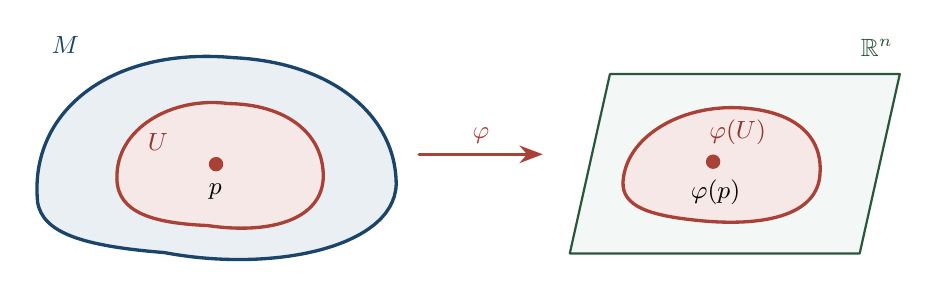
\begin{tikzpicture}[>=Stealth,scale=1.04,line cap=round,line join=round]
% Fragment M oraz wyróżniony otwarty zbiór U.
\filldraw[fill=manifoldblue!10,draw=manifoldblue!75!black,very thick]
 (-5.05,-.55) .. controls (-5.15,.55) and (-4.15,1.34) .. (-2.65,1.2)
 .. controls (-1.43,1.14) and (-.67,.48) .. (-.67,-.35)
 .. controls (-.7,-1.12) and (-2.18,-1.43) .. (-3.5,-1.18)
 .. controls (-4.5,-1.1) and (-5.0,-.94) .. cycle;
\filldraw[fill=manifoldred!12,draw=manifoldred,very thick]
 (-4.08,-.28) .. controls (-4.1,.34) and (-3.4,.73) .. (-2.72,.64)
 .. controls (-2.03,.63) and (-1.56,.29) .. (-1.56,-.25)
 .. controls (-1.57,-.79) and (-2.23,-.96) .. (-2.97,-.85)
 .. controls (-3.65,-.82) and (-4.07,-.69) .. cycle;
\node[manifoldblue!75!black,font=\small\bfseries] at (-4.71,1.35) {$M$};
\node[manifoldred!85!black,font=\small] at (-3.58,.17) {$U$};
\fill[manifoldred] (-2.87,-.1) circle (2.5pt);
\node[font=\small] at (-2.88,-.44) {$p$};
% Obraz mapy w przestrzeni współrzędnych, bez siatki.
\filldraw[fill=manifoldgreen!6,draw=manifoldgreen!70!black,thick]
 (1.45,-1.19)--(4.99,-1.19)--(5.48,1.0)--(1.94,1.0)--cycle;
\filldraw[fill=manifoldred!12,draw=manifoldred,very thick]
 (2.1,-.31) .. controls (2.14,.23) and (2.78,.6) .. (3.45,.59)
 .. controls (4.16,.58) and (4.57,.26) .. (4.5,-.27)
 .. controls (4.43,-.75) and (3.76,-.86) .. (3.04,-.79)
 .. controls (2.43,-.73) and (2.08,-.62) .. cycle;
\node[manifoldgreen!65!black,font=\small\bfseries] at (5.2,1.32) {$\R^n$};
\node[manifoldred!85!black,font=\small] at (3.5,.29) {$\varphi(U)$};
\fill[manifoldred] (3.2,-.07) circle (2.5pt);
\node[font=\small] at (3.23,-.44) {$\varphi(p)$};
\draw[->,very thick,manifoldred] (-.39,.02)--(1.12,.02)
 node[midway,above,font=\small] {$\varphi$};
\end{tikzpicture}
\caption{Mapa $(U,\varphi)$ przenosi otwarty fragment $U\subset M$ na obszar
$\varphi(U)\subset\R^n$; punktowi $p$ przyporządkowuje współrzędne $\varphi(p)$.}
\label{fig:mapa-rozmaitosc}
\end{figure}


\begin{definicja}
Dwie mapy $(U,\varphi)$ i $(V,\psi)$ na $M$ są \emph{zgodne} ($C^\infty$-zgodne), jeżeli
albo $U\cap V=\emptyset$, albo odwzorowania przejścia
\[
\psi\circ\varphi^{-1}\colon\varphi(U\cap V)\to\psi(U\cap V), \qquad
\varphi\circ\psi^{-1}\colon\psi(U\cap V)\to\varphi(U\cap V)
\]
są klasy $C^\infty$ (są to wtedy automatycznie odwzorowania wzajemnie odwrotne między
otwartymi podzbiorami $\R^n$, a więc dyfeomorfizmy).
\end{definicja}



Na Rysunku~\ref{fig:atlas-przejscie-dwie-mapy} pokazano
dwie zgodne mapy i współrzędne punktu
leżącego w ich części wspólnej. Odwzorowanie przejścia
działa \emph{między obrazami tej części wspólnej}, a nie
między całymi $\varphi_\alpha(U_\alpha)$ i
$\varphi_\beta(U_\beta)$, jeśli dziedziny map się różnią.

\begin{figure}[H]
\centering
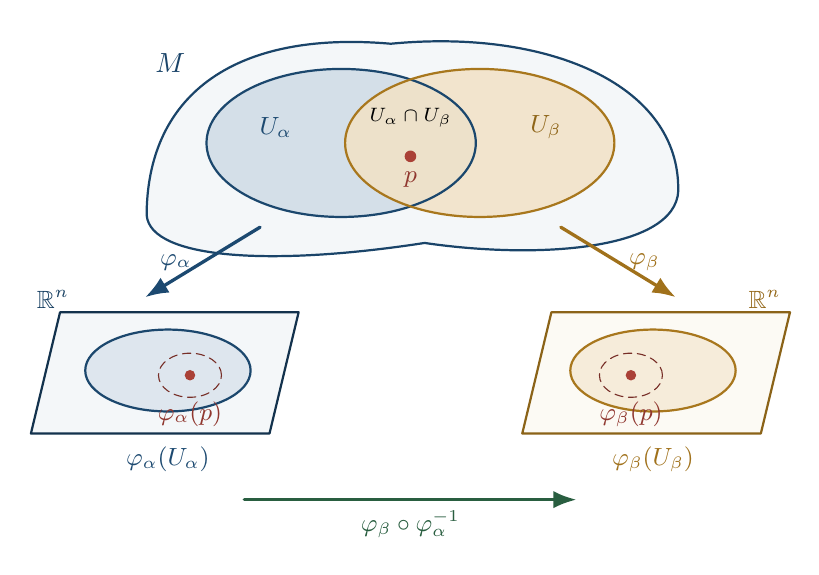
\begin{tikzpicture}[>=Latex,line cap=round,line join=round,
                     font=\small]
  % Fragment rozmaitości i dwa nakładające się obszary map.
  \filldraw[fill=manifoldblue!5,draw=manifoldblue!75!black,thick]
   (-3.35,1.25) .. controls (-3.32,2.76) and (-2.20,3.55)
   .. (-.25,3.38) .. controls (1.72,3.57) and (3.36,2.88)
   .. (3.40,1.59) .. controls (3.48,.77) and (1.68,.63)
   .. (.18,.85) .. controls (-1.90,.53) and (-3.39,.67)
   .. cycle;
  \fill[manifoldblue!22,opacity=.85]
       (-.88,2.12) ellipse (1.71 and .94);
  \fill[manifoldgold!26,opacity=.86]
       (.88,2.12) ellipse (1.71 and .94);
  \draw[manifoldblue!78!black,thick]
       (-.88,2.12) ellipse (1.71 and .94);
  \draw[manifoldgold!82!black,thick]
       (.88,2.12) ellipse (1.71 and .94);
  \node[manifoldblue!75!black,font=\bfseries] at (-3.05,3.13) {$M$};
  \node[manifoldblue!80!black] at (-1.71,2.32) {$U_\alpha$};
  \node[manifoldgold!70!black] at (1.72,2.32) {$U_\beta$};
  \node[font=\scriptsize] at (0,2.44) {$U_\alpha\cap U_\beta$};
  \fill[manifoldred] (0,1.95) circle (2.1pt);
  \node[below,manifoldred!85!black] at (0,1.88) {$p$};
  % Obrazy w dwóch osobnych przestrzeniach współrzędnych.
  \filldraw[fill=manifoldblue!5,draw=manifoldblue!55!black,thick]
       (-4.82,-1.57)--(-1.79,-1.57)--(-1.42,-.03)
       --(-4.45,-.03)--cycle;
  \fill[manifoldblue!15] (-3.08,-.77) ellipse (1.05 and .52);
  \draw[manifoldblue!78!black,thick]
       (-3.08,-.77) ellipse (1.05 and .52);
  \draw[manifoldred!70!black,densely dashed]
       (-2.80,-.83) ellipse (.40 and .28);
  \fill[manifoldred] (-2.80,-.83) circle (1.9pt);
  \node[manifoldred!85!black] at (-2.80,-1.32)
       {$\varphi_\alpha(p)$};
  \node[manifoldblue!70!black] at (-4.54,.13) {$\R^n$};

  \filldraw[fill=manifoldgold!5,draw=manifoldgold!68!black,thick]
       (1.42,-1.57)--(4.45,-1.57)--(4.82,-.03)
       --(1.79,-.03)--cycle;
  \fill[manifoldgold!17] (3.08,-.77) ellipse (1.05 and .52);
  \draw[manifoldgold!82!black,thick]
       (3.08,-.77) ellipse (1.05 and .52);
  \draw[manifoldred!70!black,densely dashed]
       (2.80,-.83) ellipse (.40 and .28);
  \fill[manifoldred] (2.80,-.83) circle (1.9pt);
  \node[manifoldred!85!black] at (2.80,-1.32)
       {$\varphi_\beta(p)$};
  \node[manifoldgold!72!black] at (4.50,.13) {$\R^n$};

  \draw[->,manifoldblue!80!black,very thick]
       (-1.91,1.05)--(-3.37,.16)
       node[midway,left] {$\varphi_\alpha$};
  \draw[->,manifoldgold!78!black,very thick]
       (1.91,1.05)--(3.37,.16)
       node[midway,right] {$\varphi_\beta$};
  \node[manifoldblue!80!black] at (-3.08,-1.90)
       {$\varphi_\alpha(U_\alpha)$};
  \node[manifoldgold!78!black] at (3.08,-1.90)
       {$\varphi_\beta(U_\beta)$};
  \draw[->,manifoldgreen!75!black,very thick]
       (-2.11,-2.41)--(2.11,-2.41)
       node[midway,below] {$\varphi_\beta\circ\varphi_\alpha^{-1}$};
\end{tikzpicture}
\caption{Dwie nakładające się mapy. Przerywane obszary
oznaczają obrazy części wspólnej. Punkt $p$ ma
dwa zapisy współrzędnych, a przejście
$\varphi_\beta\circ\varphi_\alpha^{-1}$ prowadzi
z $\varphi_\alpha(U_\alpha\cap U_\beta)$ do
$\varphi_\beta(U_\alpha\cap U_\beta)$. W atlasie
pozostałe mapy pokrywają ewentualną resztę $M$.}
\label{fig:atlas-przejscie-dwie-mapy}
\end{figure}

\begin{definicja}
\emph{Atlasem} (gładkim, $C^\infty$) na rozmaitości topologicznej $M$ nazywamy rodzinę map
$\mathcal{A}=\{(U_\alpha,\varphi_\alpha)\}_{\alpha\in I}$ taką, że:
\begin{enumerate}[label=(\roman*)]
\item $\bigcup_{\alpha\in I}U_\alpha=M$,
\item mapy $(U_\alpha,\varphi_\alpha)$ oraz $(U_\beta,\varphi_\beta)$ są zgodne dla
wszystkich $\alpha,\beta\in I$.
\end{enumerate}
\end{definicja}



Chcemy teraz porównywać różne atlasy na tej samej przestrzeni topologicznej $M$ — dwa
atlasy powinny wyznaczać tę samą strukturę gładką dokładnie wtedy, gdy razem tworzą
(większy) atlas.

\begin{definicja}
Dwa atlasy $\mathcal{A}_1$, $\mathcal{A}_2$ na $M$ są \emph{równoważne}, $\mathcal A_1\sim
\mathcal A_2$, jeżeli ich suma $\mathcal{A}_1\cup\mathcal{A}_2$ jest atlasem, tzn.\ każda
mapa z $\mathcal{A}_1$ jest zgodna z każdą mapą z $\mathcal{A}_2$.
\end{definicja}

Poniższy lemat techniczny jest kluczowym narzędziem rachunkowym tego paragrafu; wykorzystamy
go dwukrotnie: do dowodu, że $\sim$ jest relacją równoważności, oraz do dowodu istnienia i
jednoznaczności atlasu maksymalnego.

\begin{lemat}\label{lem:zgodnosc-przechodnia}
Niech $(U,\varphi)$, $(W,\eta)$, $(V,\psi)$ będą mapami na $M$ takimi, że $(U,\varphi)$
jest zgodna z $(W,\eta)$, a $(W,\eta)$ jest zgodna z $(V,\psi)$. Wówczas dla dowolnego
punktu $p\in U\cap V\cap W$, odwzorowania $\psi\circ\varphi^{-1}$ i $\varphi\circ\psi^{-1}$
są klasy $C^\infty$ w (odpowiednich) otoczeniach punktów $\varphi(p)$ i $\psi(p)$.
\end{lemat}

\begin{proof}
Na otoczeniu $\varphi(U\cap V\cap W)$ punktu $\varphi(p)$ mamy równość
$\psi\circ\varphi^{-1}=(\psi\circ\eta^{-1})\circ(\eta\circ\varphi^{-1})$; odwzorowanie
$\eta\circ\varphi^{-1}$ jest gładkie na $\varphi(U\cap W)$ (zgodność $(U,\varphi)$ z
$(W,\eta)$), a $\psi\circ\eta^{-1}$ jest gładkie na $\eta(W\cap V)$ (zgodność $(W,\eta)$ z
$(V,\psi)$); złożenie odwzorowań gładkich jest gładkie, więc $\psi\circ\varphi^{-1}$ jest
gładkie w otoczeniu $\varphi(p)$. Analogicznie, na otoczeniu $\psi(p)$:
$\varphi\circ\psi^{-1}=(\varphi\circ\eta^{-1})\circ(\eta\circ\psi^{-1})$ jest złożeniem
odwzorowań gładkich ($\varphi\circ\eta^{-1}$ i $\eta\circ\psi^{-1}$ gładkie, z tych samych
dwóch założeń zgodności), a więc gładkie.
\end{proof}

\begin{stwierdzenie}
Równoważność atlasów jest relacją równoważności na zbiorze wszystkich atlasów na $M$.
\end{stwierdzenie}

\begin{proof}
Zwrotność i symetria są oczywiste z definicji. Sprawdzimy przechodniość. Niech
$\mathcal{A}_1\sim\mathcal{A}_2$ i $\mathcal{A}_2\sim\mathcal{A}_3$; pokażemy, że
$\mathcal{A}_1\sim\mathcal{A}_3$, czyli że dowolna mapa $(U,\varphi)\in\mathcal{A}_1$ jest
zgodna z dowolną mapą $(V,\psi)\in\mathcal{A}_3$. Jeśli $U\cap V=\emptyset$, zgodność jest
trywialna. W przeciwnym razie ustalmy $p\in U\cap V$. Ponieważ $\mathcal{A}_2$ jest atlasem
pokrywającym $M$, istnieje mapa $(W,\eta)\in\mathcal{A}_2$ z $p\in W$. Z założenia
$\mathcal{A}_1\sim\mathcal{A}_2$, mapa $(U,\varphi)$ jest zgodna z $(W,\eta)$; z założenia
$\mathcal{A}_2\sim\mathcal{A}_3$, mapa $(W,\eta)$ jest zgodna z $(V,\psi)$. Na mocy
Lematu~\ref{lem:zgodnosc-przechodnia} (zastosowanego w punkcie $p\in U\cap V\cap W$),
odwzorowania $\psi\circ\varphi^{-1}$ i $\varphi\circ\psi^{-1}$ są gładkie w otoczeniach
odpowiednio $\varphi(p)$ i $\psi(p)$. Ponieważ punkt $p\in U\cap V$ był dowolny, oba te
odwzorowania są gładkie na całych swoich dziedzinach $\varphi(U\cap V)$, $\psi(U\cap V)$
(gładkość jest własnością lokalną). Zatem $(U,\varphi)$ i $(V,\psi)$ są zgodne, co dowodzi
$\mathcal{A}_1\sim\mathcal{A}_3$.
\end{proof}

W praktyce nie chcemy jednak utożsamiać struktury gładkiej z pojedynczym atlasem — dwa
równoważne atlasy powinny wyznaczać \emph{tę samą} strukturę. Wygodnie jest wybrać
kanonicznego reprezentanta każdej klasy równoważności: atlas maksymalny.

\begin{definicja}
Atlas $\mathcal{A}$ na $M$ jest \emph{maksymalny}, jeśli nie jest właściwym podzbiorem
żadnego innego atlasu na $M$, tzn.\ jeśli mapa $(U,\varphi)$ jest zgodna z każdą mapą
należącą do $\mathcal{A}$, to $(U,\varphi)\in\mathcal{A}$.
\end{definicja}

\begin{twierdzenie}\label{tw:atlas-maksymalny}
Każdy atlas $\mathcal{A}$ na $M$ jest zawarty w dokładnie jednym atlasie maksymalnym
$\mathcal{A}^+$, zadanym wzorem
\[
\mathcal{A}^+=\{(U,\varphi)\text{ -- mapa na }M : (U,\varphi)\text{ jest zgodna z każdą
mapą z }\mathcal{A}\}.
\]
Ponadto dwa atlasy $\mathcal{A}_1$, $\mathcal{A}_2$ są równoważne wtedy i tylko wtedy, gdy
$\mathcal{A}_1^+=\mathcal{A}_2^+$.
\end{twierdzenie}

\begin{proof}
\emph{Krok 1: $\mathcal{A}^+$ jest atlasem.} Ponieważ $\mathcal{A}\subseteq\mathcal{A}^+$
(każda mapa z $\mathcal{A}$ jest zgodna z każdą mapą z $\mathcal{A}$, gdyż $\mathcal{A}$
jest atlasem), zbiory dziedzin map z $\mathcal{A}^+$ pokrywają $M$. Pozostaje sprawdzić, że
dowolne dwie mapy $(U,\varphi),(V,\psi)\in\mathcal{A}^+$ są ze sobą zgodne. Ustalmy
$p\in U\cap V$ (dla $U\cap V=\emptyset$ zgodność jest trywialna); ponieważ $\mathcal{A}$
pokrywa $M$, istnieje $(W,\eta)\in\mathcal{A}$ z $p\in W$. Mapa $(U,\varphi)$ jest zgodna z
$(W,\eta)$ (bo $(U,\varphi)\in\mathcal{A}^+$ jest zgodna z każdą mapą z $\mathcal A$), a
$(W,\eta)$ jest zgodna z $(V,\psi)$ (analogicznie, bo $(V,\psi)\in\mathcal A^+$). Na mocy
Lematu~\ref{lem:zgodnosc-przechodnia}, odwzorowania $\psi\circ\varphi^{-1}$,
$\varphi\circ\psi^{-1}$ są gładkie w otoczeniach $\varphi(p)$, $\psi(p)$; wobec dowolności
$p\in U\cap V$, są gładkie na całych dziedzinach $\varphi(U\cap V)$, $\psi(U\cap V)$. Zatem
$\mathcal{A}^+$ jest atlasem.

\emph{Krok 2: $\mathcal{A}^+$ jest maksymalny.} Niech mapa $(U,\varphi)$ będzie zgodna z
każdą mapą należącą do $\mathcal{A}^+$. Ponieważ $\mathcal{A}\subseteq\mathcal{A}^+$, mapa
$(U,\varphi)$ jest w szczególności zgodna z każdą mapą z $\mathcal{A}$, a więc z definicji
$\mathcal{A}^+$ mamy $(U,\varphi)\in\mathcal{A}^+$.

\emph{Krok 3: jednoznaczność.} Niech $\mathcal B\supseteq\mathcal A$ będzie atlasem
maksymalnym. Ponieważ $\mathcal B$ jest atlasem i $\mathcal A\subseteq\mathcal B$, każda
mapa z $\mathcal B$ jest zgodna z każdą mapą z $\mathcal A$ (obie należą do atlasu
$\mathcal B$) — więc $\mathcal B\subseteq\mathcal A^+$ z definicji $\mathcal A^+$.

Odwrotnie, niech $(U,\varphi)\in\mathcal A^+$; pokażemy $(U,\varphi)\in\mathcal B$, co —
wobec dowolności $(U,\varphi)\in\mathcal A^+$ — da $\mathcal A^+\subseteq\mathcal B$, a
wraz z poprzednią inkluzją: $\mathcal B=\mathcal A^+$. Z maksymalności $\mathcal B$
wystarczy pokazać, że $(U,\varphi)$ jest zgodna z każdą mapą $(V,\psi)\in\mathcal B$.
Ustalmy taką mapę i punkt $p\in U\cap V$ (dla $U\cap V=\emptyset$ zgodność jest trywialna).
Ponieważ $\mathcal A$ pokrywa $M$, istnieje $(W,\eta)\in\mathcal A$ z $p\in W$. Mapa
$(U,\varphi)$ jest zgodna z $(W,\eta)$ (bo $(U,\varphi)\in\mathcal A^+$), a $(W,\eta)\in
\mathcal A\subseteq\mathcal B$ jest zgodna z $(V,\psi)\in\mathcal B$ (bo obie należą do
atlasu $\mathcal B$). Na mocy Lematu~\ref{lem:zgodnosc-przechodnia}, $(U,\varphi)$ i
$(V,\psi)$ są zgodne w otoczeniu $p$; wobec dowolności $p\in U\cap V$ — zgodne na całych
dziedzinach. Zatem $(U,\varphi)$ jest zgodna z każdą mapą z $\mathcal B$, więc — z
maksymalności $\mathcal B$ — $(U,\varphi)\in\mathcal B$.

\emph{Krok 4: $\mathcal A_1\sim\mathcal A_2\iff\mathcal A_1^+=\mathcal A_2^+$.}
($\Leftarrow$) Jeśli $\mathcal A_1^+=\mathcal A_2^+=:\mathcal B$, to $\mathcal A_1\subseteq
\mathcal B$ i $\mathcal A_2\subseteq\mathcal B$, a skoro $\mathcal B$ jest atlasem, każda
mapa z $\mathcal A_1$ jest zgodna z każdą mapą z $\mathcal B$, w szczególności z każdą mapą
z $\mathcal A_2$ — czyli $\mathcal A_1\sim\mathcal A_2$.

($\Rightarrow$) Załóżmy $\mathcal A_1\sim\mathcal A_2$. Pokażemy $\mathcal A_1^+\subseteq
\mathcal A_2^+$ (inkluzja odwrotna analogicznie, skąd równość). Niech $(U,\varphi)\in
\mathcal A_1^+$. Ustalmy dowolną mapę $(V,\psi)\in\mathcal A_2$ i (dla $U\cap V\neq
\emptyset$, inaczej trywialnie) punkt $p\in U\cap V$. Ponieważ $\mathcal A_1$ pokrywa $M$,
istnieje $(W,\eta)\in\mathcal A_1$ z $p\in W$. Mapa $(U,\varphi)$ jest zgodna z $(W,\eta)\in
\mathcal A_1$ (bo $(U,\varphi)\in\mathcal A_1^+$), a $(W,\eta)\in\mathcal A_1$ jest zgodna z
$(V,\psi)\in\mathcal A_2$ (bo $\mathcal A_1\sim\mathcal A_2$). Na mocy
Lematu~\ref{lem:zgodnosc-przechodnia}, $(U,\varphi)$ i $(V,\psi)$ są zgodne w otoczeniu
$p$; wobec dowolności $p\in U\cap V$ — na całych dziedzinach. Zatem $(U,\varphi)$ jest
zgodna z $(V,\psi)$; wobec dowolności $(V,\psi)\in\mathcal A_2$, mamy $(U,\varphi)\in
\mathcal A_2^+$.
\end{proof}

Powyższe twierdzenie pozwala oddzielić topologię przestrzeni od
wyboru współrzędnych, w których będziemy różniczkować.

\begin{definicja}[Struktura różniczkowa]\label{def:struktura-rozniczkowa}
\index{struktura rozniczkowa@Struktura różniczkowa}
\emph{Strukturą różniczkową} klasy $C^\infty$ na rozmaitości
topologicznej $M$ nazywamy klasę równoważności atlasów gładkich
na $M$. Równoważnie, na mocy Twierdzenia~\ref{tw:atlas-maksymalny},
jest nią jedyny atlas maksymalny $\mathcal A=\mathcal A_0^+$
zawierający dowolny atlas $\mathcal A_0$ z tej klasy. Mapy
należące do $\mathcal A$ nazywamy \emph{dopuszczalnymi}.
\end{definicja}

\begin{definicja}[Rozmaitość gładka]\label{def:rozmaitosc-gladka}
\index{rozmaitosc gladka@Rozmaitość gładka}
\emph{Rozmaitością gładką} (klasy $C^\infty$) wymiaru $n$
nazywamy parę $(M,\mathcal A)$, gdzie $M$ jest rozmaitością
topologiczną wymiaru $n$, a $\mathcal A$ jest strukturą
różniczkową zapisaną jako atlas maksymalny.
\end{definicja}

W praktyce wystarczy podać mały atlas $\mathcal A_0$:
wyznacza on jednoznacznie strukturę $\mathcal A_0^+$.
Topologia określa, które mapy współrzędnych są homeomorfizmami;
struktura różniczkowa określa dodatkowo, które przejścia
między nimi są gładkie.

\begin{przyklad}[Różne struktury na tej samej przestrzeni]
Na topologicznej prostej $\R$ atlas $\mathcal A_{\mathrm{std}}$
z mapą $\id\colon\R\to\R$ i atlas $\mathcal A_h$ z mapą
$h\colon\R\to\R$, $h(x)=x^3$, są osobno atlasami gładkimi.
Nie są równoważne: w jednym kierunku
przejście jest dane przez $h^{-1}(u)=\sqrt[3]{u}$,
które nie jest różniczkowalne w zerze.
Definiują zatem różne struktury na \emph{ustalonym} zbiorze
topologicznym $\R$, choć otrzymane rozmaitości są
dyfeomorficzne (w sensie definicji~\ref{def dyfeo}): dyfeomorfizm
$h\colon(\R,\mathcal A_h^+)\to(\R,\mathcal A_{\mathrm{std}}^+)$
ma w odpowiednich mapach współrzędnych postać identyczności.
\end{przyklad}

\begin{uwaga}[Intuicja: mapa, atlas i rozmaitość]
Najprostszym sposobem zrozumienia pojęć \emph{mapy}, \emph{atlasu} i
\emph{rozmaitości} jest analogia z powierzchnią Ziemi.

Powierzchnia Ziemi jest obiektem zakrzywionym i nie możemy przedstawić jej
w całości na jednej płaskiej kartce bez zniekształceń. Możemy jednak wybrać
niewielki fragment powierzchni, na przykład okolice Krakowa, i przedstawić go
na płaskiej mapie. Matematycznie dokładnie taką rolę pełni \emph{mapa}
rozmaitości.

Jeżeli $M$ jest rozmaitością, to mapa jest parą $(U,\varphi)$, gdzie
$U\subset M$ jest otwartym fragmentem rozmaitości, a
\[
    \varphi\colon U\longrightarrow \varphi(U)\subset\mathbb{R}^n
\]
jest homeomorfizmem. Oznacza to, że punkty znajdujące się w $U$ możemy opisać
za pomocą zwykłych współrzędnych
\[
    (x^1,\ldots,x^n)\in\mathbb{R}^n.
\]
Można więc myśleć o $\varphi$ jako o sposobie ``rozłożenia'' niewielkiego
fragmentu rozmaitości na płaskiej przestrzeni $\mathbb{R}^n$.

Jedna mapa zazwyczaj nie wystarcza do opisania całej przestrzeni. Podobnie
jedna mapa geograficzna przedstawiająca okolice Krakowa nie opisuje całej
powierzchni Ziemi. Potrzebujemy wielu map
\[
    (U_\alpha,\varphi_\alpha),
\]
których dziedziny pokrywają całą przestrzeń:
\[
    M=\bigcup_{\alpha}U_\alpha.
\]
Taki zbiór map nazywamy \emph{atlasem}.

Jeżeli dwa obszary $U_\alpha$ i $U_\beta$ nachodzą na siebie, to ten sam punkt
rozmaitości może mieć dwa różne opisy współrzędnościowe. Przejście pomiędzy
nimi opisuje odwzorowanie
\[
    \varphi_\beta\circ\varphi_\alpha^{-1},
\]
zwane odwzorowaniem przejścia. Można je porównać do przeliczania współrzędnych
tego samego miejsca pomiędzy dwiema zachodzącymi na siebie mapami
geograficznymi.

\emph{Rozmaitość} jest zatem przestrzenią, która globalnie może być
skomplikowana lub zakrzywiona, ale w dostatecznie małym otoczeniu każdego
punktu wygląda jak zwykła przestrzeń euklidesowa $\mathbb{R}^n$.

W skrócie:
\[
\boxed{
\begin{array}{ccl}
\text{mapa}      &\longleftrightarrow& \text{lokalny układ współrzędnych},\\[2mm]
\text{atlas}     &\longleftrightarrow& \text{zbiór map opisujących całą przestrzeń},\\[2mm]
\text{rozmaitość}&\longleftrightarrow& \text{przestrzeń lokalnie wyglądająca jak }\mathbb{R}^n.
\end{array}}
\]

Przykładowo sfera $S^2$ nie jest płaską częścią $\mathbb{R}^2$, ale każdy jej
dostatecznie mały fragment można opisać za pomocą dwóch współrzędnych.
Dlatego $S^2$ jest dwuwymiarową rozmaitością.
\end{uwaga}

Od tej pory, mówiąc o rozmaitości $M$, będziemy mieli na myśli rozmaitość gładką — parę
$(M,\mathcal{A})$ — pomijając $\mathcal{A}$ w oznaczeniach, gdy nie prowadzi to do
nieporozumień.

\section{Rozmaitości z brzegiem}
\label{sec:rozmaitosci-z-brzegiem-1}
\index{brzeg rozmaitosci@Brzeg rozmaitości}

Wnętrze dysku wygląda lokalnie jak otwarty zbiór w $\R^n$,
ale punkt na jego brzegu ma tylko jedną stronę. Modelem takiego
otoczenia jest półprzestrzeń
\[
 \mathbb H^n=\{(x^1,\ldots,x^n)\in\R^n:x^n\geq0\},
 \qquad n\geq1.
\]
Otwartość podzbioru $\mathbb H^n$ rozumiemy w topologii względnej.

\begin{definicja}[Rozmaitość gładka z brzegiem]
\index{rozmaitosc gladka z brzegiem@Rozmaitość gładka z brzegiem}
\label{def:rozmaitosc-z-brzegiem-1}
\emph{Rozmaitość gładka z brzegiem} wymiaru $n\geq1$ to przestrzeń
Hausdorffa spełniająca drugi aksjomat przeliczalności, wyposażona
w atlas homeomorfizmów
$\varphi_\alpha:U_\alpha\to V_\alpha$ na zbiory
$V_\alpha$ otwarte w $\mathbb H^n$. Na częściach wspólnych
odwzorowania przejścia i ich odwrotności mają być gładkie:
w otoczeniu każdego punktu rozumie się przez to istnienie
gładkiego przedłużenia na otwarty zbiór w $\R^n$.
Maksymalny atlas zgodny z tym atlasem wyznacza strukturę gładką,
tak jak w Twierdzeniu~\ref{tw:atlas-maksymalny}.
\emph{Brzegiem rozmaitości} nazywamy zbiór
\[
 \partial M=\{p\in M:\varphi_\alpha(p)^n=0
             \text{ w pewnej mapie }(U_\alpha,\varphi_\alpha)\}.
\]
Pozostałe punkty tworzą wnętrze $M^\circ=M\setminus\partial M$.
Dla wymiaru $0$ przyjmujemy $\partial M=\varnothing$.
\end{definicja}

Warunek „w pewnej mapie” jest poprawny dzięki następującemu
faktowi; jednocześnie pokazuje, że brzeg nie zależy od wyboru
współrzędnych.

\begin{stwierdzenie}[Niezależność brzegu od mapy]
\label{prop:brzeg-niezalezny-1}
Dla $n\geq1$, jeśli $p$ ma ostatnią współrzędną równą $0$ w jednej
mapie półprzestrzennej, to ma ją równą $0$ w każdej
mapie półprzestrzennej, której dziedzina zawiera $p$.
Zbiór $\partial M$ jest zamknięty w $M$ i z map ograniczonych
do $\partial M$ otrzymuje strukturę gładkiej
rozmaitości wymiaru $n-1$ bez brzegu.
\end{stwierdzenie}
\begin{proof}
Przypuśćmy, że $\varphi(p)$ leży na płaszczyźnie
$x^n=0$, a $\psi(p)$ jest punktem wnętrza $\mathbb H^n$.
Ograniczmy mapy do wspólnego dostatecznie małego otoczenia
$p$. Wtedy $\psi$ odwzorowuje je na zbiór otwarty w $\R^n$,
a $\varphi\circ\psi^{-1}$ jest ciągłą injekcją tego zbioru
do $\R^n$. Twierdzenie Brouwera o niezmienniczości obszaru
orzeka, że obraz takiej injekcji jest otwarty w $\R^n$.
Obraz leży jednak w $\mathbb H^n$ i zawiera punkt
$\varphi(p)$ na jego płaszczyźnie brzegowej, więc nie może
być otwarty w $\R^n$. Sprzeczność dowodzi pierwszej tezy.
Dokładne sformułowanie użytego wyniku zewnętrznego podaje
\href{https://pi.math.cornell.edu/~hatcher/AT/AT.pdf}
{A. Hatcher, \emph{Algebraic Topology}, twierdzenie 2B.3}.

W każdej mapie punkty z $x^n>0$ tworzą zbiór otwarty.
Zatem $M^\circ$ jest otwarty, a $\partial M$ zamknięty.
Ograniczenie mapy $\varphi$ do
$U\cap\partial M$ przyjmuje wartości w otwartym
podzbiorze $\R^{n-1}\times\{0\}$. Przejścia między
tymi ograniczeniami są gładkie, bo są ograniczeniami
gładkich przedłużeń przejść na $\R^n$; to samo dotyczy
odwrotności. Są to więc mapy gładkiej rozmaitości
wymiaru $n-1$. Każda z nich ma obraz otwarty w całej
$\R^{n-1}$, czyli $\partial M$ nie ma własnego brzegu.
\end{proof}

W punkcie brzegu definiujemy $T_pM$ przez
wektory współrzędnych w półprzestrzennej mapie,
równoważnie przez derywacje gładkich kiełków
funkcji w $p$. Pełną konstrukcję i niezależność od przedłużeń
podamy po wprowadzeniu przestrzeni stycznej, w
Stwierdzeniu~\ref{prop:styczna-brzeg-1}. Ten model ma $n$ niezależnych
kierunków: $T_pM\cong\R^n$, natomiast
$T_p\partial M\cong\{v\in\R^n:v^n=0\}$ ma wymiar $n-1$.
Wektor o ujemnej ostatniej współrzędnej należy do $T_pM$,
choć nie jest prędkością krzywej biegnącej od $p$ do wnętrza
przy dodatnim czasie. Przykładowo $T_0[0,1]\cong\R$,
podczas gdy $T_0\partial[0,1]=0$.
Model przez krzywe określone na otwartym przedziale,
omówiony w Sekcji~\ref{sec:przestrzen-styczna},
dotyczy punktów wnętrza: w punkcie brzegu
dwustronna krzywa w $M$ nie reprezentuje
kierunku poprzecznego do brzegu.

\begin{przyklad}[Kula, okrąg i brzeg otaczającej przestrzeni]
\label{prz:brzeg-kula-okrag-1}
Domknięta kula $D^n=\{x\in\R^n:|x|\leq1\}$ ma brzeg
rozmaitościowy $S^{n-1}$. Rzeczywiście, przy $|p|=1$
funkcja $\rho(x)=1-|x|^2$ ma niezerową różniczkę
$\dd\rho_p(v)=-2\langle p,v\rangle$. Twierdzenie o funkcji
odwrotnej pozwala użyć $\rho$ jako ostatniej lokalnej
współrzędnej, zatem $D^n$ odpowiada warunkowi $\rho\geq0$.
Z kolei brzeg okręgu $S^1\subset\R^2$ jako rozmaitości
(w sensie Definicji~\ref{def:rozmaitosc-z-brzegiem-1})
jest pusty: $\partial S^1=\varnothing$. Jego brzeg topologiczny
jako \emph{podzbioru $\R^2$} jest natomiast całym $S^1$: okrąg ma
puste wnętrze w $\R^2$ i jest domknięty.
Te dwa znaczenia słowa „brzeg” trzeba odróżniać.
\end{przyklad}

Produkt dwóch rozmaitości z brzegiem może mieć
\emph{naroża}. W kwadracie $[0,1]^2$ przy wierzchołku
naturalny model pochodzący z zanurzenia to
$[0,\infty)^2$, z dwiema ścianami brzegowymi.
W rachunku uchwytów spotkamy taki model na
$\partial D^k\times\partial D^{n-k}$; naroże można
zaokrąglić w małym otoczeniu, zachowując części
odległe od niego. To operacja na gładkiej geometrii
brzegu, a nie zmiana tego, które punkty są brzegowe
topologicznie. Kołnierze i takie zaokrąglanie pojawią się
w Sekcji~\ref{sec:kolnierz-15} i przy uchwytach w
Sekcji~\ref{sec:uchwyt-morse-17}.

\section{Rozmaitości zespolone}

Analogicznie do konstrukcji z poprzedniego paragrafu, możemy modelować rozmaitość lokalnie
nie na $\R^n$, lecz na $\C^n$, żądając przy tym, by odwzorowania przejścia między mapami
były holomorficzne, a nie tylko gładkie.

\begin{definicja}
\emph{Rozmaitością zespoloną} wymiaru (zespolonego) $n$ nazywamy przestrzeń Hausdorffa $M$
spełniającą drugi aksjomat przeliczalności, wyposażoną w atlas $\{(U_\alpha,\varphi_\alpha)\}$
map $\varphi_\alpha\colon U_\alpha\to\varphi_\alpha(U_\alpha)\subseteq\C^n$ (homeomorfizmów
na zbiory otwarte w $\C^n\cong\R^{2n}$), takich że odwzorowania przejścia
\[
\varphi_\beta\circ\varphi_\alpha^{-1}\colon\varphi_\alpha(U_\alpha\cap U_\beta)\to
\varphi_\beta(U_\alpha\cap U_\beta)
\]
są \emph{holomorficzne} (jako odwzorowania między otwartymi podzbiorami $\C^n$), wraz z
maksymalnym takim atlasem (konstrukcja atlasu maksymalnego przebiega dosłownie tak samo,
jak w Sekcji~\ref{sec:atlas}, z ,,gładki'' zastąpionym przez ,,holomorficzny'' — złożenie odwzorowań
holomorficznych jest holomorficzne, więc Lemat~\ref{lem:zgodnosc-przechodnia} i
Twierdzenie~\ref{tw:atlas-maksymalny} przenoszą się bez zmian).
\end{definicja}

\begin{uwaga}
Utożsamiając $\C^n\cong\R^{2n}$ (przez część rzeczywistą i urojoną każdej współrzędnej)
oraz przypominając, że każde odwzorowanie holomorficzne jest w szczególności odwzorowaniem
gładkim (klasy $C^\infty$) w sensie rzeczywistym (ze wzoru całkowego
Cauchy'ego na małym polidysku wynika lokalne rozwinięcie w szereg potęgowy,
który można różniczkować wyraz po wyrazie), widzimy, że \emph{każda rozmaitość zespolona
wymiaru $n$ jest w naturalny sposób rzeczywistą rozmaitością gładką wymiaru $2n$}. Implikacja
odwrotna jest fałszywa: nie każda parzystowymiarowa rozmaitość gładka dopuszcza strukturę
zespoloną (a nawet jeśli dopuszcza, struktura taka zwykle nie jest jednoznaczna).
\end{uwaga}

\begin{przyklad}[Zespolona przestrzeń rzutowa]
Niech $\C_*:=\C\setminus\{0\}$ oznacza zbiór niezerowych
liczb zespolonych.
Zespolonym odpowiednikiem $\mathbb{RP}^n$ z
Przykładu~\ref{prz:RPn} jest przestrzeń ilorazowa
\[
\mathbb{CP}^n
:=
(\C^{n+1}\setminus\{0\})/\!\sim,
\]
gdzie
\[
z\sim w
\iff
\exists\,\lambda\in\C_*
\quad\text{takie, że}\quad
z=\lambda w.
\]
Przestrzeń $\mathbb{CP}^n$ wyposażamy w topologię ilorazową.
Punkty zapisujemy w postaci
\[
[z^0:z^1:\dots:z^n],
\]
przy czym
\[
[z^0:\dots:z^n]
=
[\lambda z^0:\dots:\lambda z^n]
\qquad
\text{dla każdego }\lambda\in\C_*.
\]

Dla $i=0,\dots,n$ definiujemy
\[
U_i
=
\{[z^0:\dots:z^n]\in\mathbb{CP}^n:z^i\neq0\}.
\]
Zbiory $U_i$ są otwarte i pokrywają całą przestrzeń $\mathbb{CP}^n$.
Na każdym z nich definiujemy mapę
\[
\varphi_i:U_i\longrightarrow\C^n
\]
wzorem
\[
\varphi_i([z^0:\dots:z^n])
=
\left(
\frac{z^0}{z^i},
\dots,
\frac{z^{i-1}}{z^i},
\frac{z^{i+1}}{z^i},
\dots,
\frac{z^n}{z^i}
\right).
\]
Jej odwrotność jest dana jawnie przez
\[
\varphi_i^{-1}
(w^0,\dots,w^{i-1},w^{i+1},\dots,w^n)
=
[w^0:\dots:w^{i-1}:1:w^{i+1}:\dots:w^n].
\]
Sprawdźmy także ciągłość, której nie daje sama bijektywność.
Niech $\pi\colon\C^{n+1}\setminus\{0\}\to\mathbb{CP}^n$ będzie
rzutowaniem ilorazowym. Przeciwobraz $\pi^{-1}(U_i)=\{z:z^i\ne0\}$
jest otwarty, zatem $U_i$ jest otwarty. Ograniczenie
$\pi\colon\pi^{-1}(U_i)\to U_i$ także jest odwzorowaniem ilorazowym:
otwarty w $\pi^{-1}(U_i)$ przeciwobraz podzbioru $U_i$ jest otwarty
w całej dziedzinie $\pi$, więc sam podzbiór jest otwarty w ilorazie.
Składowe $\varphi_i\circ\pi$ są ciągłymi ilorazami współrzędnych;
z własności topologii ilorazowej wynika ciągłość $\varphi_i$.
Podany wzór na $\varphi_i^{-1}$ jest złożeniem ciągłego wstawienia
współrzędnej $1$ z $\pi$. Każda $\varphi_i$ jest więc homeomorfizmem
pomiędzy $U_i$ a $\C^n$.

Na przecięciu $U_i\cap U_j$ ten sam punkt przestrzeni
$\mathbb{CP}^n$ posiada dwa różne opisy współrzędnościowe.
Przejście pomiędzy nimi jest opisane przez odwzorowanie
\[
\varphi_j\circ\varphi_i^{-1}.
\]
Jego składowe są ilorazami wielomianów zespolonych, przy czym
mianowniki nie znikają na dziedzinie odwzorowania. Odwzorowania
przejścia są zatem holomorficzne. Aksjomat Hausdorffa i istnienie
przeliczalnej bazy topologii sprawdzimy w dowodzie
twierdzenia~\ref{thm:rzutowe-zwarte-1}. Łącznie daje to strukturę
rozmaitości zespolonej wymiaru $n$ na $\mathbb{CP}^n$, a więc również
rzeczywistej rozmaitości gładkiej wymiaru $2n$.

Rozważmy teraz szczególny przypadek $n=1$. Otrzymujemy
\emph{sferę Riemanna}
\[
\mathbb{CP}^1.
\]
Mamy wówczas dwa zbiory
\[
U_0=\{[z^0:z^1]:z^0\neq0\},
\qquad
U_1=\{[z^0:z^1]:z^1\neq0\},
\]
oraz mapy
\[
\varphi_0:U_0\longrightarrow\C,
\qquad
\varphi_0([z^0:z^1])=\frac{z^1}{z^0},
\]
i
\[
\varphi_1:U_1\longrightarrow\C,
\qquad
\varphi_1([z^0:z^1])=\frac{z^0}{z^1}.
\]
Każda z tych map identyfikuje odpowiedni fragment
$\mathbb{CP}^1$ z kopią płaszczyzny zespolonej $\C$.

Na przecięciu
\[
U_0\cap U_1
=
\{[z^0:z^1]:z^0\neq0,\ z^1\neq0\}
\]
ten sam punkt ma w pierwszej mapie współrzędną
\[
w
=
\varphi_0([z^0:z^1])
=
\frac{z^1}{z^0},
\]
natomiast w drugiej mapie współrzędną
\[
v
=
\varphi_1([z^0:z^1])
=
\frac{z^0}{z^1}.
\]
Stąd
\[
v=\frac1w.
\]
Odwzorowanie przejścia ma więc postać
\[
\varphi_1\circ\varphi_0^{-1}(w)
=
\frac1w,
\qquad
w\in\C_*.
\]

Możemy zatem patrzeć na $\mathbb{CP}^1$ jako na przestrzeń otrzymaną
z dwóch rozłącznych kopii płaszczyzny zespolonej,
\[
\C_0\sqcup\C_1,
\]
przez utożsamienie punktów należących do ich niezerowych części zgodnie
z regułą
\[
w\in\C_0\setminus\{0\}
\quad\sim\quad
\frac1w\in\C_1\setminus\{0\}.
\]
W tym właśnie sensie mówi się, że dwie kopie $\C$ są
\emph{sklejone za pomocą odwzorowania przejścia}
\[
w\longmapsto\frac1w.
\]
Nie sklejamy więc całych płaszczyzn punkt po punkcie, lecz utożsamiamy
jedynie te punkty obu kopii $\C$, które odpowiadają temu samemu punktowi
przestrzeni $\mathbb{CP}^1$ na części wspólnej $U_0\cap U_1$.

Punkt $0\in\C_0$ odpowiada punktowi
\[
[1:0]\in\mathbb{CP}^1,
\]
natomiast punkt $0\in\C_1$ odpowiada punktowi
\[
[0:1]\in\mathbb{CP}^1.
\]
W szczególności, patrząc wyłącznie przez mapę $\varphi_0$, punkt
$[0:1]$ można interpretować jako dodatkowy punkt w nieskończoności.
Dlatego często zapisuje się
\[
\mathbb{CP}^1
\cong
\C\cup\{\infty\}.
\]

Przestrzeń $\mathbb{CP}^1$ jest dyfeomorficzna ze sferą $S^2$.
Trzeba jednak uważać na wybór zespolonych współrzędnych
stereograficznych. Zwykłe rzeczywiste rzuty stereograficzne z
Przykładu~\ref{prz:sfera}, po utożsamieniu $\R^2=\C$, prowadzą do
odwzorowania przejścia
\[
w\longmapsto\frac{w}{|w|^2}
=
\frac1{\overline{w}},
\]
które nie jest holomorficzne.

Aby otrzymać strukturę zespoloną zgodną ze strukturą na
$\mathbb{CP}^1$, wybieramy na $S^2$ współrzędne
\[
\zeta_N(x)
=
\frac{x^1+ix^2}{1-x^3},
\qquad
\zeta_S(x)
=
\frac{x^1-ix^2}{1+x^3}.
\]
Wtedy na części wspólnej zachodzi
\[
\zeta_S\circ\zeta_N^{-1}(w)
=
\frac1w.
\]

Jawny dyfeomorfizm
\[
H:\mathbb{CP}^1\longrightarrow S^2
\]
jest dany wzorem
\[
H([z^0:z^1])
=
\frac{
\big(
2\operatorname{Re}(\overline{z^0}z^1),
2\operatorname{Im}(\overline{z^0}z^1),
|z^1|^2-|z^0|^2
\big)
}{
|z^0|^2+|z^1|^2
}.
\]
Skalowanie obu współrzędnych przez $\lambda\neq0$ mnoży licznik
i mianownik przez $|\lambda|^2$, dlatego wzór jest dobrze określony
na klasach równoważności.

Ponadto
\[
4|z^0|^2|z^1|^2
+
\big(|z^1|^2-|z^0|^2\big)^2
=
\big(|z^0|^2+|z^1|^2\big)^2,
\]
co pokazuje, że obraz odwzorowania $H$ leży na sferze $S^2$.

W wybranych współrzędnych mamy
\[
\zeta_N\circ H=\varphi_0,
\qquad
\zeta_S\circ H=\varphi_1.
\]
Pierwsza z tych równości daje bijekcję
\[
U_0\longrightarrow S^2\setminus\{N\},
\]
natomiast pozostały punkt
\[
[0:1]
\]
przechodzi na biegun północny $N$.
W lokalnych współrzędnych odwzorowanie $H$ oraz jego odwrotność są
tożsamościami, co pokazuje, że
\[
\mathbb{CP}^1\cong S^2
\]
jako rozmaitości gładkie.
\end{przyklad}


\begin{figure}[h]
\centering
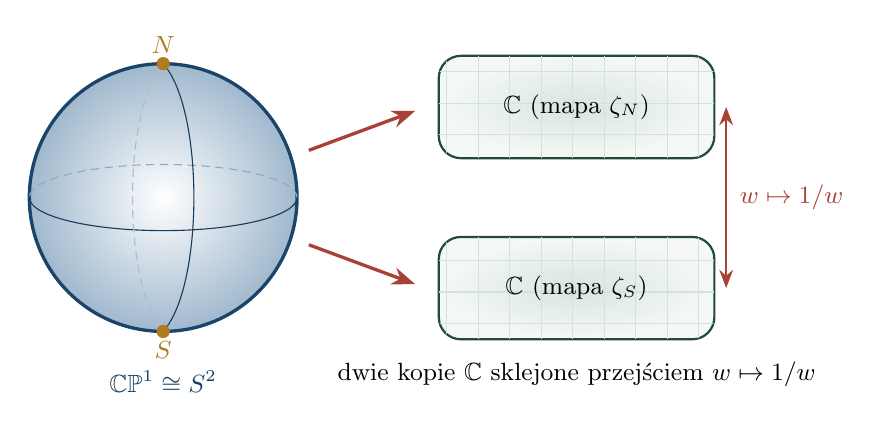
\begin{tikzpicture}[>=Stealth,scale=1]
% Sfera: jasna plama i podział równika na część widoczną oraz ukrytą.
\shade[inner color=white,outer color=manifoldblue!43] (0,0) circle (1.7);
\draw[manifoldblue!75!black,very thick] (0,0) circle (1.7);
\draw[manifoldblue!52,densely dashed,thin]
  (1.7,0) arc[start angle=0,end angle=180,x radius=1.7,y radius=.42];
\draw[manifoldblue!65!black,thin]
  (-1.7,0) arc[start angle=180,end angle=360,x radius=1.7,y radius=.42];
\draw[manifoldblue!40,densely dashed,thin] (0,1.7)
  .. controls (-.52,1.12) and (-.52,-1.12) .. (0,-1.7);
\draw[manifoldblue!65!black,thin] (0,1.7)
  .. controls (.52,1.12) and (.52,-1.12) .. (0,-1.7);
% bieguny
\fill[manifoldgold!85!black] (0,1.7) circle (2.4pt) node[above,font=\small]{$N$};
\fill[manifoldgold!85!black] (0,-1.7) circle (2.4pt) node[below,font=\small]{$S$};
\node[manifoldblue!70!black,font=\small] at (0,-2.35) {$\mathbb{CP}^1\cong S^2$};
% --- strzałki do płaszczyzn C ---
\draw[->,very thick,manifoldred] (1.85,0.6) -- (3.2,1.1);
\draw[->,very thick,manifoldred] (1.85,-0.6) -- (3.2,-1.1);
% --- dwie kopie C (zaokrąglone) ---
% górna
\shade[inner color=manifoldgreen!20, outer color=manifoldgreen!5, rounded corners=8pt]
  (3.5,0.5) rectangle (7.0,1.8);
\draw[manifoldgreen!60!black,thick,rounded corners=8pt]
  (3.5,0.5) rectangle (7.0,1.8);
\begin{scope}
  \clip[rounded corners=8pt] (3.5,0.5) rectangle (7.0,1.8);
  \draw[step=0.4,manifoldgreen!22,thin] (3.5,0.5) grid (7.0,1.8);
\end{scope}
\node[font=\small] at (5.25,1.15) {$\C$ (mapa $\zeta_N$)};
% dolna
\shade[inner color=manifoldgreen!20, outer color=manifoldgreen!5, rounded corners=8pt]
  (3.5,-1.8) rectangle (7.0,-0.5);
\draw[manifoldgreen!60!black,thick,rounded corners=8pt]
  (3.5,-1.8) rectangle (7.0,-0.5);
\begin{scope}
  \clip[rounded corners=8pt] (3.5,-1.8) rectangle (7.0,-0.5);
  \draw[step=0.4,manifoldgreen!22,thin] (3.5,-1.8) grid (7.0,-0.5);
\end{scope}
\node[font=\small] at (5.25,-1.15) {$\C$ (mapa $\zeta_S$)};
% przejście w↦1/w
\draw[<->,thick,manifoldred] (7.15,1.15) -- (7.15,-1.15);
\node[manifoldred,font=\small,right] at (7.2,0) {$w\mapsto 1/w$};
\node[font=\small] at (5.25,-2.25) {dwie kopie $\C$ sklejone przejściem $w\mapsto 1/w$};
\end{tikzpicture}
\caption{Schematyczna interpretacja $\mathbb{CP}^1$ jako sfery Riemanna:
dwie mapy zespolone pokrywają sferę; w mapie południowej odwrócono
znak drugiej współrzędnej rzeczywistej. Przejście $1/w$ jest określone dla $w\ne0$.}
\label{fig:cp1}
\end{figure}

\section{Odwzorowania gładkie między rozmaitościami}

\begin{definicja}
Niech $M$, $N$ będą rozmaitościami gładkimi wymiarów odpowiednio $m$, $n$. Odwzorowanie
$F\colon M\to N$ jest \emph{gładkie} (klasy $C^\infty$) w punkcie $p\in M$, jeżeli dla
pewnej (równoważnie: każdej) mapy dopuszczalnej $(U,\varphi)$ wokół $p$ i mapy
dopuszczalnej $(V,\psi)$ wokół $F(p)$ z $F(U)\subseteq V$, odwzorowanie
\[
\psi\circ F\circ\varphi^{-1}\colon\varphi(U)\to\psi(V)
\]
jest gładkie (klasy $C^\infty$) w pewnym otwartym otoczeniu
$\varphi(p)$. Odwzorowanie $F$ jest gładkie, jeśli jest gładkie w każdym punkcie $p\in M$.
Zbiór wszystkich gładkich funkcji $M\to\R$ oznaczamy $C^\infty(M)$.
\end{definicja}
\begin{figure}[ht]
\centering
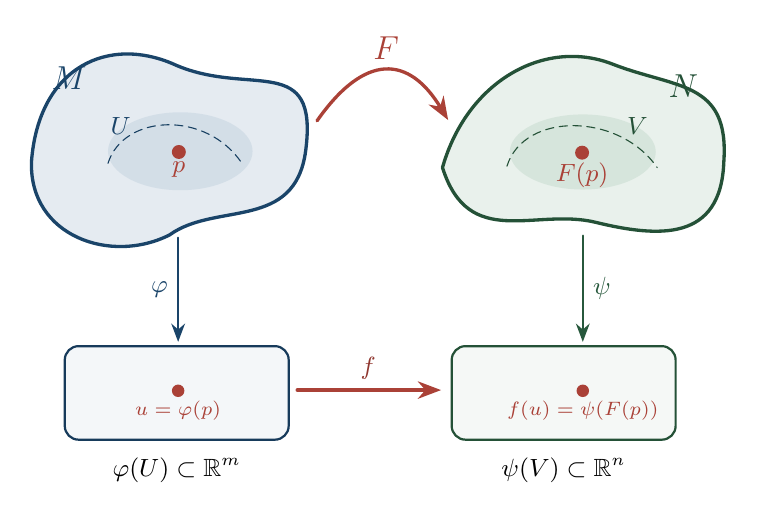
\begin{tikzpicture}[>=Stealth,scale=.9,line cap=round,line join=round]
% Dwie pofalowane powierzchnie z siatką lokalnych współrzędnych.
\def\Mshape{(-4.75,.2) .. controls (-4.65,1.55) and (-3.65,2.0) .. (-2.7,1.56)
 .. controls (-1.65,1.12) and (-.7,1.75) .. (-.88,.36)
 .. controls (-1.03,-.78) and (-2.15,-.36) .. (-2.8,-.83)
 .. controls (-3.63,-1.25) and (-4.78,-.85) .. cycle}
\def\Nshape{(1.05,.12) .. controls (1.4,1.35) and (2.5,1.95) .. (3.45,1.58)
 .. controls (4.35,1.23) and (5.1,1.35) .. (5.02,.2)
 .. controls (4.98,-.93) and (4.1,-.87) .. (3.2,-.65)
 .. controls (2.35,-.45) and (1.42,-1.05) .. cycle}
\fill[manifoldblue!12] \Mshape;
\begin{scope}
\clip \Mshape;
\fill[manifoldblue!24,opacity=.65] (-2.65,.35) ellipse (1.02 and .55);
\end{scope}
\draw[manifoldblue!75!black,very thick] \Mshape;
\draw[manifoldblue!70!black,densely dashed] (-3.67,.18) .. controls (-3.45,.88) and (-2.28,.93) .. (-1.78,.18);
\fill[manifoldgreen!11] \Nshape;
\begin{scope}
\clip \Nshape;
\fill[manifoldgreen!25,opacity=.65] (3.03,.34) ellipse (1.03 and .53);
\end{scope}
\draw[manifoldgreen!65!black,very thick] \Nshape;
\draw[manifoldgreen!65!black,densely dashed] (1.96,.14) .. controls (2.2,.91) and (3.54,.9) .. (4.08,.12);
\node[font=\large\bfseries,manifoldblue!75!black] at (-4.22,1.38) {$M$};
\node[font=\large\bfseries,manifoldgreen!65!black] at (4.45,1.27) {$N$};
\node[font=\small,manifoldblue!75!black] at (-3.49,.7) {$U$};
\node[font=\small,manifoldgreen!65!black] at (3.8,.7) {$V$};
\fill[manifoldred] (-2.67,.34) circle (2.8pt) node[below,font=\small] {$p$};
\fill[manifoldred] (3.02,.33) circle (2.8pt) node[below,font=\small] {$F(p)$};
\draw[->,very thick,manifoldred] (-.72,.78) .. controls (-.04,1.75) and (.58,1.7) .. (1.13,.79)
  node[midway,above,font=\large\bfseries] {$F$};
% Dwie euklidesowe mapy z zaznaczonymi odpowiadającymi sobie punktami.
\fill[manifoldblue!5,rounded corners=5pt] (-4.28,-3.72) rectangle (-1.12,-2.4);
\draw[manifoldblue!65!black,thick,rounded corners=5pt] (-4.28,-3.72) rectangle (-1.12,-2.4);
\fill[manifoldgreen!5,rounded corners=5pt] (1.18,-3.72) rectangle (4.34,-2.4);
\draw[manifoldgreen!65!black,thick,rounded corners=5pt] (1.18,-3.72) rectangle (4.34,-2.4);
\draw[->,thick,manifoldblue!75!black] (-2.68,-.87)--(-2.68,-2.34)
  node[midway,left,font=\small] {$\varphi$};
\draw[->,thick,manifoldgreen!70!black] (3.03,-.84)--(3.03,-2.34)
  node[midway,right,font=\small] {$\psi$};
\fill[manifoldred] (-2.68,-3.03) circle (2.5pt) node[below,font=\scriptsize] {$u=\varphi(p)$};
\fill[manifoldred] (3.03,-3.03) circle (2.5pt) node[below,font=\scriptsize] {$f(u)=\psi(F(p))$};
\draw[->,very thick,manifoldred] (-1.0,-3.02)--(1.03,-3.02);
\node[font=\small\bfseries,manifoldred!85!black] at (0,-2.71) {$f$};
\node[font=\small] at (-2.7,-4.15) {$\varphi(U)\subset\R^m$};
\node[font=\small] at (2.76,-4.15) {$\psi(V)\subset\R^n$};
\end{tikzpicture}
\caption{Odwzorowanie $F\colon M\to N$ oraz jego lokalny zapis współrzędnościowy. Po wybraniu map $(U,\varphi)$ i $(V,\psi)$ gładkość $F$ bada się poprzez zwykłe odwzorowanie $\psi\circ F\circ\varphi^{-1}$ między otwartymi podzbiorami przestrzeni euklidesowych.}
\label{fig:odwzorowanie-gładkie}
\end{figure}

\begin{uwaga}
Definicja gładkości nie zależy od wyboru map. Niech $(U,\varphi)$ oraz
$(V,\psi)$ będą mapami wokół odpowiednio $p$ i $F(p)$, dla których
odwzorowanie
\[
\psi\circ F\circ\varphi^{-1}
\]
jest gładkie. Jeśli $(U',\varphi')$, $(V',\psi')$ są innymi mapami
dopuszczalnymi wokół $p$ i $F(p)$, to chcemy porównać oba opisy
współrzędnościowe funkcji $F$.

Najpierw zauważmy, że na odpowiednio małym otoczeniu punktu $p$ mamy
\[
F
=
\psi^{-1}\circ
(\psi\circ F\circ\varphi^{-1})
\circ\varphi.
\]
Ponieważ $\varphi$ i $\psi^{-1}$ są homeomorfizmami, a odwzorowanie
$\psi\circ F\circ\varphi^{-1}$ jest gładkie, a więc w szczególności
ciągłe, otrzymujemy, że $F$ jest ciągłe w pewnym otoczeniu punktu $p$.

Ponieważ
\[
p\in U\cap U'
\qquad\text{oraz}\qquad
F(p)\in V\cap V',
\]
a $V\cap V'$ jest zbiorem otwartym, wybierzmy otwarte otoczenie
$O$ punktu $p$, na którym $F$ jest ciągłe. Wówczas
\[
(F|_O)^{-1}(V\cap V')=O\cap F^{-1}(V\cap V')
\]
jest otwartym otoczeniem $p$ w $M$. Możemy więc zmniejszyć dziedzinę
do otwartego otoczenia
\[
W\subseteq O\cap U\cap U'\cap F^{-1}(V\cap V').
\]
Na $W$ jednocześnie obowiązują oba układy współrzędnych, a obraz
$F(W)$ jest zawarty w $V\cap V'$. Wszystkie poniższe złożenia są zatem
dobrze określone.

Na odpowiadającej zbiorowi $W$ dziedzinie mamy
\[
\psi'\circ F\circ(\varphi')^{-1}
=
(\psi'\circ\psi^{-1})
\circ
(\psi\circ F\circ\varphi^{-1})
\circ
(\varphi\circ(\varphi')^{-1}).
\]
Odwzorowania
\[
\varphi\circ(\varphi')^{-1}
\qquad\text{oraz}\qquad
\psi'\circ\psi^{-1}
\]
są odwzorowaniami przejścia, a więc są gładkie z definicji zgodności
map. Co więcej, są one dyfeomorfizmami pomiędzy odpowiednimi otwartymi
podzbiorami przestrzeni euklidesowych. Zatem złożenie z nimi nie zmienia
gładkości. W konsekwencji
\[
\psi'\circ F\circ(\varphi')^{-1}
\]
jest gładkie wtedy i tylko wtedy, gdy gładkie jest
\[
\psi\circ F\circ\varphi^{-1}.
\]
Definicja gładkości odwzorowania $F$ nie zależy więc od wyboru map
w dziedzinie i przeciwdziedzinie.
\end{uwaga}

\begin{definicja}\label{def dyfeo}
Odwzorowanie gładkie $F\colon M\to N$ jest \emph{dyfeomorfizmem}, jeśli jest bijekcją, a
$F^{-1}\colon N\to M$ jest również gładkie. Rozmaitości $M$, $N$ nazywamy
\emph{dyfeomorficznymi}, jeśli istnieje między nimi dyfeomorfizm.
\end{definicja}

\begin{stwierdzenie}
Złożenie odwzorowań gładkich jest gładkie: jeśli $F\colon M\to N$ i $G\colon N\to P$ są
gładkie, to $G\circ F\colon M\to P$ jest gładkie.
\end{stwierdzenie}

\begin{proof}
Ustalmy $p\in M$ i mapy dopuszczalne $(U,\varphi)$ wokół $p$, $(V,\psi)$ wokół $F(p)$,
$(W,\eta)$ wokół $G(F(p))$, z $F(U)\subseteq V$, $G(V)\subseteq W$ (istnienie takich map —
po ewentualnym zmniejszeniu $V$, a następnie $U$ — wynika z ciągłości $F$ i $G$, którą zapewnia gładkość).
Wówczas na $\varphi(U)$
\[
\eta\circ(G\circ F)\circ\varphi^{-1}=(\eta\circ G\circ\psi^{-1})\circ(\psi\circ F\circ
\varphi^{-1}),
\]
czyli złożenie dwóch odwzorowań gładkich (między otwartymi podzbiorami przestrzeni
euklidesowych) — a takie złożenie jest gładkie na mocy zwykłego twierdzenia analizy wielu
zmiennych o różniczkowaniu złożenia.
\end{proof}
\section{Przykłady rozmaitości}

\begin{stwierdzenie}\label{stw:otwarty-podzbior}
Jeśli $M$ jest rozmaitością gładką wymiaru $n$ i $\Omega\subseteq M$ jest zbiorem otwartym,
to $\Omega$ z topologią i strukturą gładką odziedziczoną po $M$ (mapy $(U\cap\Omega,
\varphi|_{U\cap\Omega})$ dla map dopuszczalnych $(U,\varphi)$ na $M$) jest rozmaitością
gładką wymiaru $n$.
\end{stwierdzenie}

\begin{proof}
Warunki Hausdorffa i drugiej przeliczalności dziedziczą się automatycznie na
podprzestrzenie. Rodzina $\{(U\cap\Omega,\varphi|_{U\cap\Omega})\}$, gdzie $(U,\varphi)$
przebiega atlas maksymalny na $M$, pokrywa $\Omega$ (bo mapy pokrywają $M\supseteq\Omega$)
i składa się z homeomorfizmów na zbiory otwarte $\varphi(U\cap\Omega)\subseteq\varphi(U)
\subseteq\R^n$ (obraz zbioru otwartego $U\cap\Omega$ przez homeomorfizm $\varphi$ jest
otwarty w $\varphi(U)$, a więc i w $\R^n$). Zgodność map $(U\cap\Omega,\varphi|_{U\cap
\Omega})$ i $(U'\cap\Omega,\varphi'|_{U'\cap\Omega})$ wynika natychmiast ze zgodności
$(U,\varphi)$ i $(U',\varphi')$, gdyż odwzorowania przejścia dla map obciętych są
obcięciami odwzorowań przejścia dla map oryginalnych do (otwartego) podzbioru dziedziny.
\end{proof}

\begin{przyklad}
Zbiór $\mathrm{GL}(n,\R)$ macierzy odwracalnych $n\times n$ o wyrazach rzeczywistych jest
otwartym podzbiorem przestrzeni $M_n(\R)\cong\R^{n^2}$ wszystkich macierzy $n\times n$ (bo
$\det\colon M_n(\R)\to\R$ jest funkcją ciągłą, a $\mathrm{GL}(n,\R)=\det^{-1}(\R\setminus
\{0\})$ jest przeciwobrazem zbioru otwartego). Na mocy Stwierdzenia~\ref{stw:otwarty-podzbior},
$\mathrm{GL}(n,\R)$ jest rozmaitością gładką wymiaru $n^2$.
\end{przyklad}

\begin{stwierdzenie}[Rozmaitość produktowa]
Jeśli $M$, $N$ są rozmaitościami gładkimi wymiarów odpowiednio $m$, $n$, to $M\times N$
(z topologią produktową) jest rozmaitością gładką wymiaru $m+n$, z atlasem złożonym z map
$(U\times V,\varphi\times\psi)$, gdzie $(U,\varphi)$ jest mapą na $M$, a $(V,\psi)$ mapą na
$N$, i $(\varphi\times\psi)(p,q):=(\varphi(p),\psi(q))\in\R^m\times\R^n\cong\R^{m+n}$.
\end{stwierdzenie}

\begin{proof}
Hausdorffowość i druga przeliczalność produktu dwóch przestrzeni o tych własnościach są
standardowymi faktami z topologii ogólnej. Mapy $\varphi\times\psi$ są homeomorfizmami na
zbiory otwarte jako produkty homeomorfizmów na zbiory otwarte, a ich dziedziny pokrywają
$M\times N$. Jeśli $(U_1\times V_1,\varphi_1\times\psi_1)$ i $(U_2\times V_2,\varphi_2
\times\psi_2)$ są dwiema takimi mapami, ich odwzorowanie przejścia to
\[
(\varphi_2\times\psi_2)\circ(\varphi_1\times\psi_1)^{-1}=(\varphi_2\circ\varphi_1^{-1})
\times(\psi_2\circ\psi_1^{-1}),
\]
które jest gładkie jako produkt dwóch odwzorowań gładkich. Zatem otrzymana rodzina map
jest atlasem.
\end{proof}

\begin{przyklad}[Sfera $S^n$ przez rzuty stereograficzne]\label{prz:sfera}
Niech $S^n=\{x\in\R^{n+1}:\|x\|=1\}$ z topologią podprzestrzeni $\R^{n+1}$. Oznaczmy przez
$N=(0,\dots,0,1)$ i $S=(0,\dots,0,-1)$ bieguny północny i południowy. Definiujemy rzut
stereograficzny z bieguna północnego,
\[
\varphi_N\colon S^n\setminus\{N\}\to\R^n, \qquad
\varphi_N(x^1,\dots,x^{n+1})=\frac{1}{1-x^{n+1}}(x^1,\dots,x^n),
\]
tzn.\ $\varphi_N(x)$ to punkt przecięcia prostej przechodzącej przez $N$ i $x$ z
hiperpłaszczyzną $\{x^{n+1}=0\}\cong\R^n$. Odwzorowanie odwrotne wyraża się wzorem
\[
\varphi_N^{-1}(u)=\frac1{\|u\|^2+1}\big(2u,\ \|u\|^2-1\big)\in\R^n\times\R,
\]
co sprawdzamy bezpośrednim rachunkiem: punkt $y=\varphi_N^{-1}(u)$ leży na prostej
$t\mapsto(tu,1-t)$ (parametryzacja prostej przez $N=(0,1)$ w kierunku $(u,0)-N=(u,-1)$) i
spełnia $\|y\|=1$; rozwiązując $t^2\|u\|^2+(1-t)^2=1$, tzn.\ $t\big(t(\|u\|^2+1)-2\big)=0$,
względem $t\neq0$, otrzymujemy $t=2/(\|u\|^2+1)$, skąd powyższy wzór. Analogicznie
definiujemy $\varphi_S\colon S^n\setminus\{S\}\to\R^n$, rzut z bieguna południowego, wzorem
$\varphi_S(x)=\frac1{1+x^{n+1}}(x^1,\dots,x^n)$.

Zbiory $S^n\setminus\{N\}$ i $S^n\setminus\{S\}$ pokrywają $S^n$, więc pozostaje sprawdzić
gładkość odwzorowania przejścia na $\varphi_N(S^n\setminus\{N,S\})=\R^n\setminus\{0\}$.
Podstawiając $\varphi_N^{-1}(u)$ do wzoru na $\varphi_S$, i licząc osobno mianownik
\[
1+\frac{\|u\|^2-1}{\|u\|^2+1}=\frac{2\|u\|^2}{\|u\|^2+1},
\]
otrzymujemy
\[
(\varphi_S\circ\varphi_N^{-1})(u)=\frac{2u/(\|u\|^2+1)}{2\|u\|^2/(\|u\|^2+1)}=
\frac{u}{\|u\|^2},
\]
czyli inwersja względem sfery jednostkowej. Odwzorowanie $u\mapsto u/\|u\|^2$ jest gładkie
na $\R^n\setminus\{0\}$, a jest ono swoją własną odwrotnością (dla $w=u/\|u\|^2$ mamy
$\|w\|^2=1/\|u\|^2$, więc $w/\|w\|^2=(u/\|u\|^2)\cdot\|u\|^2=u$), więc obie mapy są
zgodne. Zatem $\{(S^n\setminus\{N\},\varphi_N),(S^n\setminus\{S\},\varphi_S)\}$ jest
atlasem na $S^n$, nadającym jej strukturę rozmaitości gładkiej wymiaru $n$.
\end{przyklad}

\begin{figure}[ht]
\centering
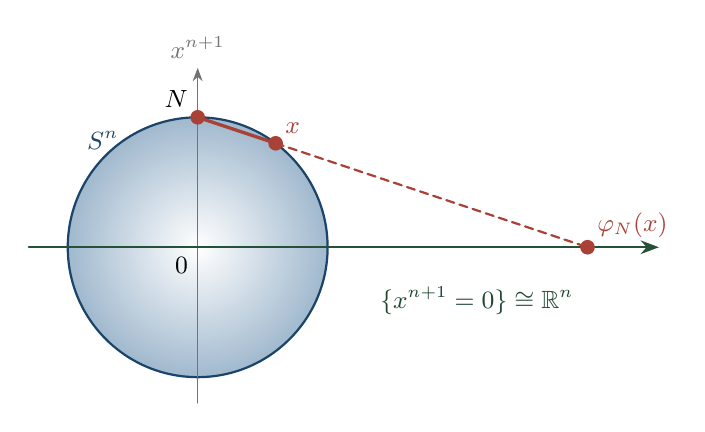
\begin{tikzpicture}[>=Stealth,scale=1.65,line cap=round,line join=round]
\shade[inner color=white,outer color=manifoldblue!43] (0,0) circle (1);
\draw[manifoldblue!75!black,thick] (0,0) circle (1);
\draw[->,black!55] (0,-1.2)--(0,1.38) node[above,font=\small] {$x^{n+1}$};
\draw[->,manifoldgreen!65!black,thick] (-1.3,0)--(3.55,0);
\node[below,font=\small,manifoldgreen!55!black] at (2.15,-.23)
 {$\{x^{n+1}=0\}\cong\R^n$};
\coordinate (N) at (0,1);
\coordinate (X) at (.6,.8);
\coordinate (P) at (3,0);
\draw[manifoldred,very thick] (N)--(X);
\draw[manifoldred,thick,densely dashed] (X)--(P);
\foreach \name in {N,X,P}{\fill[manifoldred] (\name) circle (1.6pt);}
\node[above left,font=\small] at (N) {$N$};
\node[above right,font=\small,manifoldred] at (X) {$x$};
\node[above right,font=\small,manifoldred] at (P) {$\varphi_N(x)$};
\node[below left,font=\small] at (0,0) {$0$};
\node[manifoldblue!75!black,font=\small] at (-.73,.82) {$S^n$};
\end{tikzpicture}
\caption{Rzut stereograficzny na płaszczyznę równikową, zgodny ze wzorem
w tekście. Pokazano przekrój płaszczyzną zawierającą oś biegunową
i punkt $x$. Punkty $N,x,\varphi_N(x)$ leżą na jednej prostej;
punkt przecięcia z $\{x^{n+1}=0\}$ ma współrzędne
$\varphi_N(x)=(x^1,\ldots,x^n)/(1-x^{n+1})$.}
\label{fig:stereo}
\end{figure}


\begin{przyklad}[Rzeczywista przestrzeń rzutowa]\label{prz:RPn}
Niech $\R_*:=\R\setminus\{0\}$ oznacza zbiór niezerowych
liczb rzeczywistych.
Niech
\[
\mathbb{RP}^n
=
(\R^{n+1}\setminus\{0\})/\!\sim,
\]
gdzie
\[
x\sim y
\iff
\exists\,\lambda\in\R_*
\quad\text{takie, że}\quad
x=\lambda y.
\]
Przestrzeń $\mathbb{RP}^n$ wyposażamy w topologię ilorazową względem
rzutowania
\[
\pi:\R^{n+1}\setminus\{0\}\longrightarrow\mathbb{RP}^n,
\qquad
\pi(x)=[x].
\]
Punkty przestrzeni rzutowej zapisujemy w postaci
\[
[x^0:\dots:x^n].
\]

Dla $i=0,\dots,n$ definiujemy
\[
U_i
=
\{[x^0:\dots:x^n]\in\mathbb{RP}^n:x^i\neq0\}.
\]
Najpierw należy sprawdzić, że definicja ta nie zależy od wyboru
reprezentanta klasy $[x]$. Jeżeli $x\sim y$, to istnieje
$\lambda\neq0$ takie, że $y=\lambda x$, a więc
\[
y^i=\lambda x^i.
\]
Ponieważ $\lambda\neq0$, mamy
\[
x^i\neq0
\iff
y^i\neq0.
\]
Warunek $x^i\neq0$ zależy zatem wyłącznie od klasy $[x]$, więc zbiór
$U_i$ jest dobrze określony.

Zauważmy następnie, że
\[
\pi^{-1}(U_i)
=
\{x\in\R^{n+1}\setminus\{0\}:x^i\neq0\}.
\]
Jest to zbiór otwarty w $\R^{n+1}\setminus\{0\}$, ponieważ jest
przeciwobrazem otwartego zbioru
$\R_*$ przez ciągłą funkcję współrzędnościową
\[
x\longmapsto x^i.
\]
Z definicji topologii ilorazowej zbiór $A\subseteq\mathbb{RP}^n$
jest otwarty wtedy i tylko wtedy, gdy $\pi^{-1}(A)$ jest otwarty
w $\R^{n+1}\setminus\{0\}$. Stąd każdy $U_i$ jest otwarty.

Ponieważ każdy niezerowy wektor
$x=(x^0,\dots,x^n)$ ma przynajmniej jedną niezerową współrzędną,
zbiory $U_i$ pokrywają całą przestrzeń:
\[
\mathbb{RP}^n
=
\bigcup_{i=0}^n U_i.
\]

Na $U_i$ definiujemy odwzorowanie
\[
\varphi_i:U_i\longrightarrow\R^n
\]
wzorem
\[
\varphi_i([x^0:\dots:x^n])
=
\left(
\frac{x^0}{x^i},
\dots,
\frac{x^{i-1}}{x^i},
\frac{x^{i+1}}{x^i},
\dots,
\frac{x^n}{x^i}
\right),
\]
czyli po znormalizowaniu reprezentanta tak, aby jego $i$-ta
współrzędna była równa $1$, pomijamy tę współrzędną.

Także tutaj należy sprawdzić niezależność od wyboru reprezentanta.
Jeżeli $y=\lambda x$ dla pewnego $\lambda\neq0$, to dla każdego
$j\neq i$ mamy
\[
\frac{y^j}{y^i}
=
\frac{\lambda x^j}{\lambda x^i}
=
\frac{x^j}{x^i}.
\]
Wartość $\varphi_i([x])$ zależy więc wyłącznie od klasy $[x]$.

Odwzorowanie odwrotne jest dane jawnie przez wstawienie $1$
na $i$-te miejsce:
\[
\varphi_i^{-1}
(u^0,\dots,u^{i-1},u^{i+1},\dots,u^n)
=
[u^0:\dots:u^{i-1}:1:u^{i+1}:\dots:u^n].
\]
W szczególności $\varphi_i$ jest bijekcją.

Odwrotność $\varphi_i^{-1}$ jest ciągła, ponieważ jest złożeniem
ciągłego odwzorowania
\[
(u^0,\dots,u^{i-1},u^{i+1},\dots,u^n)
\longmapsto
(u^0,\dots,u^{i-1},1,u^{i+1},\dots,u^n)
\]
z ciągłym rzutowaniem ilorazowym $\pi$.

Aby wykazać ciągłość $\varphi_i$, zauważmy, że na zbiorze
\[
\pi^{-1}(U_i)=\{x^i\neq0\}
\]
mamy
\[
\varphi_i\circ\pi(x)
=
\left(
\frac{x^0}{x^i},
\dots,
\frac{x^{i-1}}{x^i},
\frac{x^{i+1}}{x^i},
\dots,
\frac{x^n}{x^i}
\right),
\]
a więc $\varphi_i\circ\pi$ jest ciągłe. Ponieważ obcięcie
\[
\pi|_{\pi^{-1}(U_i)}:
\pi^{-1}(U_i)\longrightarrow U_i
\]
jest odwzorowaniem ilorazowym, wynika stąd ciągłość $\varphi_i$.
Otrzymujemy zatem homeomorfizm
\[
\varphi_i:U_i\longrightarrow\R^n.
\]

Pozostaje sprawdzić zgodność map. Dla $i\neq j$ na przecięciu
$U_i\cap U_j$ odwzorowanie przejścia
\[
\varphi_j\circ\varphi_i^{-1}
\]
jest określone tam, gdzie współrzędna odpowiadająca ilorazowi
$x^j/x^i$ jest niezerowa. Każda jego składowa jest albo odwrotnością
tej współrzędnej, albo ilorazem jednej ze współrzędnych przez nią.
Są to zatem funkcje wymierne o nieznikającym na dziedzinie
mianowniku, a więc funkcje gładkie.

W konsekwencji
\[
\{(U_i,\varphi_i)\}_{i=0}^n
\]
jest atlasem gładkim. Po sprawdzeniu aksjomatów topologicznych
w twierdzeniu poniżej otrzymujemy, że $\mathbb{RP}^n$ jest
rozmaitością gładką wymiaru $n$.
\end{przyklad}


\begin{przyklad}[Dwie mapy $\mathbb{RP}^2$ krok po kroku]\label{prz:RP2-przejscie-1}
Na $U_0$ każda klasa ma jednoznacznego reprezentanta
\[
[1:u:v],
\]
natomiast na $U_1$ ma reprezentanta
\[
[a:1:b].
\]
Ich część wspólna $U_0\cap U_1$, zapisana we współrzędnych mapy
$\varphi_0$, odpowiada warunkowi $u\neq0$. Aby przejść od współrzędnych
zadanych przez $\varphi_0$ do współrzędnych zadanych przez $\varphi_1$,
dzielimy trzy współrzędne jednorodne przez $u$:
\[
[1:u:v]
=
[1/u:1:v/u].
\]
Stąd odwzorowanie zmiany współrzędnych ma postać
\[
\varphi_1\circ\varphi_0^{-1}(u,v)
=
\left(\frac1u,\frac vu\right).
\]
Oznacza to, że jeżeli punkt $p\in U_0\cap U_1$ ma w pierwszej mapie
współrzędne
\[
\varphi_0(p)=(u,v),
\]
to w drugiej mapie jego współrzędne wynoszą
\[
\varphi_1(p)=(a,b)
=
\left(\frac1u,\frac vu\right).
\]

Dziedziną odwzorowania przejścia jest
\[
\{(u,v)\in\R^2:u\neq0\},
\]
a jego macierz Jacobiego wynosi
\[
D(\varphi_1\circ\varphi_0^{-1})(u,v)
=
\begin{pmatrix}
-u^{-2} & 0\\[1mm]
-vu^{-2} & u^{-1}
\end{pmatrix}.
\]
Ponieważ
\[
\det D(\varphi_1\circ\varphi_0^{-1})(u,v)
=
-u^{-3}\neq0,
\]
a odwrotne przejście ma postać
\[
(a,b)\longmapsto
\left(\frac1a,\frac ba\right),
\]
odwzorowanie przejścia jest dyfeomorfizmem.

Zmianę współrzędnych wektora stycznego w tych mapach obliczymy
w przykładzie~\ref{prz:RP2-styczna-1}, po zdefiniowaniu przestrzeni stycznej.
\end{przyklad}


\begin{uwaga}[Geometryczna interpretacja $\mathbb{RP}^1$ i $\mathbb{RP}^2$]
Przestrzeń $\mathbb{RP}^n$ można interpretować jako zbiór prostych
przechodzących przez początek układu współrzędnych w $\R^{n+1}$.
Rzeczywiście, punkt
\[
[x^0:\dots:x^n]\in\mathbb{RP}^n
\]
odpowiada prostej
\[
\ell_x=\{\lambda x:\lambda\in\R\}.
\]
Zmiana reprezentanta $x$ na $\mu x$, gdzie $\mu\neq0$, nie zmienia tej
prostej. Współrzędne jednorodne opisują więc nie konkretny punkt
$\R^{n+1}$, lecz kierunek prostej przechodzącej przez $0$.

Każda taka prosta przecina sferę jednostkową $S^n$ w dokładnie dwóch
punktach antypodalnych $x$ i $-x$. Stąd
\[
\mathbb{RP}^n\cong S^n/\{x\sim-x\}.
\]
Jest to także identyfikacja topologii. Oznaczmy pierwotne rzutowanie
przez $\pi$ i jego ograniczenie do sfery przez $q$.
Normalizacja $\nu(x)=x/\|x\|$ jest ciągła i $\pi=q\circ\nu$.
Jeśli $q^{-1}(A)$ jest otwarty w sferze, to
$\pi^{-1}(A)=\nu^{-1}(q^{-1}(A))$ jest otwarty, zatem $A$ jest
otwarty w pierwotnej topologii ilorazowej. Odwrotna implikacja
wynika z ciągłości $q$. Stąd $q$ jest odwzorowaniem ilorazowym,
co uzasadnia powyższy homeomorfizm.

Dla $n=1$ otrzymujemy
\[
\mathbb{RP}^1\cong S^1/\{z\sim-z\}.
\]
Po utożsamieniu $S^1$ z okręgiem jednostkowym w $\C$ rozważmy
odwzorowanie
\[
F:S^1\to S^1,\qquad F(z)=z^2.
\]
Ponieważ
\[
F(z)=F(-z),
\]
odwzorowanie to jest stałe na parach antypodalnych i wyznacza
odwzorowanie
\[
\widetilde F:\mathbb{RP}^1\to S^1,
\qquad
\widetilde F([z])=z^2.
\]
Jest ono bijekcją, ponieważ
\[
z^2=w^2
\iff
z=\pm w,
\]
a każdy punkt okręgu posiada dwa przeciwne pierwiastki kwadratowe.
Ciągłość $\widetilde F$ wynika z ciągłości $F=\widetilde F\circ q$
i własności ilorazu. Ponieważ $\mathbb{RP}^1=q(S^1)$ jest zwarta,
a $S^1$ jest przestrzenią Hausdorffa, $\widetilde F$ jest homeomorfizmem.

Jest to również dyfeomorfizm. Jeśli
\[
z=e^{i\theta},
\]
to w $\mathbb{RP}^1$ kąty $\theta$ i $\theta+\pi$ opisują ten sam punkt,
natomiast
\[
\widetilde F([e^{i\theta}])=e^{2i\theta}.
\]
Sprawdźmy zgodność współrzędnych kątowych z podanym wcześniej atlasem.
Dla $[\cos\theta:\sin\theta]$, na małym przedziale z $\cos\theta\ne0$,
współrzędną afiniczną jest $\tan\theta$, o pochodnej $1/\cos^2\theta$.
Gdy $\sin\theta\ne0$, druga mapa daje $\cot\theta$, o pochodnej
$-1/\sin^2\theta$. Pochodne nie znikają, więc przejścia i ich lokalne
odwrotności są gładkie. Kąt jest zatem zgodną lokalną współrzędną.
W lokalnych współrzędnych kątowych odwzorowanie ma więc postać
\[
\theta\longmapsto 2\theta,
\]
a jego lokalna odwrotność
\[
\alpha\longmapsto \frac{\alpha}{2}.
\]
Oba odwzorowania są gładkie, zatem
\[
\mathbb{RP}^1\cong S^1
\]
jako rozmaitości gładkie.

Dla $n=2$ otrzymujemy
\[
\mathbb{RP}^2\cong S^2/\{x\sim-x\}.
\]
Możemy ograniczyć się do domkniętej półsfery północnej. Każda para
antypodalna spoza równika ma dokładnie jeden punkt w jej wnętrzu; na równiku
oba punkty pary należą do półsfery. Ponieważ domknięta półsfera jest
homeomorficzna z dyskiem $D^2$, otrzymujemy model
\[
\mathbb{RP}^2
\cong
D^2/\{x\sim-x\text{ dla }x\in\partial D^2\}.
\]
Oznacza to, że punkty wewnętrzne dysku pozostają różne, natomiast każdy
punkt brzegu utożsamiamy z punktem antypodalnym. Rzutowanie półsfery
na $\mathbb{RP}^2$ jest ciągłą surjekcją i ma dokładnie te włókna.
Wyznacza zatem ciągłą bijekcję z opisanego ilorazu dysku.
Jej dziedzina jest zwarta, a $\mathbb{RP}^2$ jest przestrzenią Hausdorffa
na mocy twierdzenia~\ref{thm:rzutowe-zwarte-1}; jest więc homeomorfizmem.

Model ten daje również intuicję, dlaczego $\mathbb{RP}^2$ nie jest
orientowalna. Wyobraźmy sobie małą strzałkę lub niewielką figurę
asymetryczną przesuwaną po dysku. Gdy dochodzimy do brzegu, przechodzimy
przez niego dzięki utożsamieniu z punktem leżącym po przeciwnej stronie
okręgu. Po takim przejściu kierunek wzdłuż brzegu pozostaje zgodny,
natomiast kierunek wskazujący do wnętrza dysku zostaje odwrócony.

Lokalnie można to zapisać schematycznie jako
\[
(s,t)\longmapsto (s,-t),
\]
gdzie $s$ oznacza kierunek wzdłuż brzegu, a $t$ kierunek poprzeczny.
Jedna z dwóch lokalnych współrzędnych zmienia więc zwrot. Po przejściu
wzdłuż odpowiedniej zamkniętej drogi wracamy do punktu początkowego
z odwróconą lokalną orientacją. Nie można zatem wybrać orientacji
w sposób zgodny na całej przestrzeni.

Jest to geometryczna intuicja nieorientowalności $\mathbb{RP}^2$;
formalny dowód podamy po wprowadzeniu pojęcia orientacji rozmaitości.
\end{uwaga}


\begin{figure}[h]
\centering
\begin{tikzpicture}[>=Stealth,scale=1]

  %-------------------- RP^1 --------------------
  \begin{scope}
    % Okrąg
    \draw[thick,manifoldblue] (0,0) circle (1.45);

    % Kilka par antypodalnych na okręgu
    \foreach \ang in {0,45,90,135}{
        \draw[dashed,gray!55]
            (\ang:1.45) -- ({\ang+180}:1.45);

        \fill[manifoldgold]
            (\ang:1.45) circle (2.2pt);
        \fill[manifoldgold]
            ({\ang+180}:1.45) circle (2.2pt);
    }

    % Wyróżniona para x i -x
    \fill[manifoldred] (20:1.45) circle (2.8pt);
    \fill[manifoldred] (200:1.45) circle (2.8pt);

    \node[manifoldred, above right] at (20:1.45) {$x$};
    \node[manifoldred, below left] at (200:1.45) {$-x$};

    % Strzałka pokazująca utożsamienie wyróżnionej pary
    \draw[<->,thick,manifoldred]
      (20:1.36) to[bend left=18] (200:1.36);

    % Opisy
    \node[manifoldblue] at (0,1.85) {$S^1$};

    \node[align=center,manifoldred] at (0,-1.95)
      {$x\sim -x$ dla każdego $x\in S^1$};

    \node at (0,-2.35)
      {$\displaystyle \mathbb{RP}^1\cong S^1/\{x\sim -x\}$};

    \node at (0,-2.75)
      {$\displaystyle \cong\, S^1$};
  \end{scope}

  %-------------------- RP^2 --------------------
  \begin{scope}[xshift=6.2cm]
    % Dysk
    \fill[manifoldblue!8] (0,0) circle (1.45);
    \draw[thick,manifoldblue] (0,0) circle (1.45);

    % Kilka przykładowych par punktów antypodalnych na brzegu
    \foreach \ang in {0,45,90,135}{
        \fill[manifoldgold]
            (\ang:1.45) circle (2.2pt);
        \fill[manifoldgold]
            ({\ang+180}:1.45) circle (2.2pt);
    }

    % Wyróżniona para x i -x
    \fill[manifoldred] (0:1.45) circle (2.8pt);
    \fill[manifoldred] (180:1.45) circle (2.8pt);

    \node[manifoldred, right] at (0:1.45) {$x$};
    \node[manifoldred, left]  at (180:1.45) {$-x$};

    % Strzałka pokazująca utożsamienie
    \draw[<->,thick,manifoldred]
        (1.36,0) to[bend left=20] (-1.36,0);
    \node[align=center,font=\scriptsize,manifoldblue] at (0,0.55)
        {wnętrze bez\\utożsamień};

    % Opisy
    \node[manifoldblue] at (0,1.85) {$D^2$};

    \node[align=center,manifoldred] at (0,-1.95)
        {$x\sim -x$ dla każdego $x\in\partial D^2$};

    \node at (0,-2.35)
        {$\displaystyle \mathbb{RP}^2
        \cong D^2/\{x\sim -x,\;x\in\partial D^2\}$};
  \end{scope}

\end{tikzpicture}
\caption{Dwa użyteczne modele przestrzeni rzutowych.
Po lewej, $\mathbb{RP}^1$ otrzymujemy z okręgu $S^1$ przez utożsamienie
par antypodalnych punktów. Po prawej, $\mathbb{RP}^2$ otrzymujemy z dysku
$D^2$ przez utożsamienie antypodalnych punktów jego brzegu. Różnica polega
na tym, że w pierwszym przypadku utożsamiamy punkty na całym okręgu,
natomiast w drugim utożsamienie zachodzi tylko na brzegu dysku.}
\label{fig:projective-models}
\end{figure}


\begin{twierdzenie}[Przestrzenie rzutowe jako zwarte rozmaitości]\label{thm:rzutowe-zwarte-1}
Przestrzeń $\mathbb{RP}^n$ jest zwartą rozmaitością gładką wymiaru $n$, a
$\mathbb{CP}^n$ jest zwartą rozmaitością zespoloną wymiaru $n$ (a więc zwartą
rozmaitością rzeczywistą wymiaru $2n$).
\end{twierdzenie}

\begin{proof}
Zaczniemy od zwartości. Niech
\[
\pi_{\R}:\R^{n+1}\setminus\{0\}\longrightarrow\mathbb{RP}^n,
\qquad
\pi_{\R}(x)=[x],
\]
będzie rzutowaniem ilorazowym. Ograniczając je do sfery jednostkowej,
otrzymujemy ciągłe odwzorowanie
\[
q_{\R}:S^n\longrightarrow\mathbb{RP}^n,
\qquad
q_{\R}(x)=[x].
\]
Jest ono surjektywne. Istotnie, jeśli
\[
[x]\in\mathbb{RP}^n,
\]
to $x\neq0$ i możemy znormalizować reprezentanta:
\[
\widehat{x}:=\frac{x}{\|x\|}\in S^n.
\]
Ponieważ $\widehat{x}$ jest niezerową wielokrotnością $x$, mamy
\[
[\widehat{x}]=[x].
\]
Każdy punkt $\mathbb{RP}^n$ należy więc do obrazu $q_{\R}$.

Sfera $S^n$ jest zwarta, a ciągły obraz przestrzeni zwartej jest zwarty.
Ponieważ
\[
q_{\R}(S^n)=\mathbb{RP}^n,
\]
otrzymujemy, że $\mathbb{RP}^n$ jest zwarta.

Dokładnie ten sam argument działa w przypadku zespolonym. Niech
\[
\pi_{\C}:\C^{n+1}\setminus\{0\}\longrightarrow\mathbb{CP}^n,
\qquad
\pi_{\C}(z)=[z].
\]
Po utożsamieniu $\C^{n+1}\cong\R^{2n+2}$ sfera jednostkowa ma postać
\[
S^{2n+1}
=
\{z\in\C^{n+1}:\|z\|=1\}.
\]
Ograniczenie
\[
q_{\C}:S^{2n+1}\longrightarrow\mathbb{CP}^n,
\qquad
q_{\C}(z)=[z],
\]
jest ciągłe i surjektywne, ponieważ dla każdego $[z]\in\mathbb{CP}^n$
wektor
\[
\widehat{z}:=\frac{z}{\|z\|}
\]
należy do $S^{2n+1}$ i reprezentuje tę samą klasę:
\[
[\widehat{z}]=[z].
\]
Ponieważ $S^{2n+1}$ jest zwarta, jej ciągły obraz
\[
q_{\C}(S^{2n+1})=\mathbb{CP}^n
\]
jest zwarty. Zatem również $\mathbb{CP}^n$ jest zwarta.

Sprawdźmy teraz aksjomat Hausdorffa bez powoływania się na ogólne
twierdzenie o ilorazach. Dla jednostkowych reprezentantów $x,y\in S^n$
dwóch klas rzeczywistych połóżmy
\[
d_{\R}([x],[y])
=
\min\{\|x-y\|,\|x+y\|\}.
\]
Dla jednostkowych reprezentantów $z,w\in S^{2n+1}$ połóżmy
\[
d_{\C}([z],[w])
=
\min_{|\lambda|=1}\|z-\lambda w\|.
\]
Oba wzory nie zależą od wyboru jednostkowych reprezentantów:
w przypadku rzeczywistym zmiana $x$ na $-x$ jedynie zamienia miejscami
dwie liczby występujące w minimum, natomiast w przypadku zespolonym
zmiana reprezentanta przez czynnik o module $1$ jedynie zmienia
parametryzację zbioru, po którym bierzemy minimum. Minima istnieją
dzięki zwartości grup $\{\pm1\}$ i $S^1$.

Nierówność trójkąta sprawdzimy jednocześnie dla obu przypadków,
pisząc $G=\{\pm1\}$ lub $G=S^1$. Dla jednostkowych $x,y,z$
wybierzmy $\lambda,\mu\in G$ realizujące minima dla par $(x,y)$ i $(y,z)$.
Ponieważ mnożenie przez $\lambda$ zachowuje normę,
\begin{align*}
d([x],[z])&\leq\|x-\lambda\mu z\|\\
&\leq\|x-\lambda y\|+\|\lambda y-\lambda\mu z\|\\
&=d([x],[y])+d([y],[z]).
\end{align*}
Symetria wynika z zastąpienia $\lambda$ przez $\lambda^{-1}$.
Ponadto osiągane minimum jest równe zeru wtedy i tylko wtedy,
gdy reprezentanty należą do tej samej orbity, czyli reprezentują
ten sam punkt przestrzeni rzutowej. Otrzymujemy więc metryki na zbiorach klas.

Pozostaje sprawdzić, że topologie wyznaczone przez te metryki są
topologiami ilorazowymi. Rzutowania
\[
q_{\R}:S^n\to(\mathbb{RP}^n,d_{\R}),
\qquad
q_{\C}:S^{2n+1}\to(\mathbb{CP}^n,d_{\C})
\]
są ciągłe, ponieważ odległość klas nie przekracza odległości ich
wybranych reprezentantów. Aby przejść od sfer do pierwotnych ilorazów,
używamy ciągłej normalizacji $\nu(v)=v/\|v\|$.
Rzutowania $\pi_{\R}$ i $\pi_{\C}$ do przestrzeni klas z metryką są ciągłe,
bo mają postać $q_{\R}\circ\nu$ i $q_{\C}\circ\nu$.
Z definicji topologii ilorazowej wynika więc ciągłość identyczności
z pierwotnego ilorazu do przestrzeni metrycznej.
Z drugiej strony mamy już wykazaną zwartość
$\mathbb{RP}^n$ i $\mathbb{CP}^n$ w ich topologiach ilorazowych.
Identyczność z przestrzeni rzutowej wyposażonej w topologię ilorazową
do tego samego zbioru klas wyposażonego w powyższą metrykę jest więc
ciągłą bijekcją ze zwartej przestrzeni do przestrzeni Hausdorffa.
Jest zatem homeomorfizmem. W szczególności pierwotna topologia
ilorazowa jest Hausdorffa.

Każda z przestrzeni rzutowych ma skończony atlas
\[
U_0,\ldots,U_n,
\]
którego obrazy są równe odpowiednio $\R^n$ lub $\C^n$. Wybierzmy
w $\R^n$ oraz $\C^n\cong\R^{2n}$ przeliczalną bazę, na przykład
złożoną z kul o wymiernych środkach i wymiernych promieniach.
Przeciwobrazy tych baz przez skończenie wiele map atlasu tworzą
przeliczalną bazę przestrzeni rzutowej.

Odwzorowania przejścia są ilorazami współrzędnych przez współrzędną
niezerową, a więc są gładkie w przypadku rzeczywistym i holomorficzne
w przypadku zespolonym. Otrzymujemy zatem strukturę rozmaitości
gładkiej wymiaru $n$ na $\mathbb{RP}^n$ oraz strukturę rozmaitości
zespolonej wymiaru $n$ na $\mathbb{CP}^n$. Ponieważ
\[
\C^n\cong\R^{2n},
\]
$\mathbb{CP}^n$ ma jako rozmaitość rzeczywista wymiar $2n$.
\end{proof}


\begin{uwaga}
Zwartość można zobaczyć bardzo bezpośrednio: każde $\mathbb{RP}^n$ jest ilorazem
sfery $S^n$ przez relację $x\sim-x$, a $\mathbb{CP}^n$ jest ilorazem sfery
jednostkowej $S^{2n+1}\subset\C^{n+1}$ przez działanie grupy $S^1$,
\[
z\sim e^{i\theta}z.
\]
W przypadku zespolonym otrzymujemy w ten sposób słynną fibrację Hopfa
\[
S^1\longrightarrow S^{2n+1}\longrightarrow\mathbb{CP}^n.
\]
Pełny opis tej konstrukcji wykracza poza zakres tego rozdziału, ale pokazuje,
że przestrzenie rzutowe są naturalnie związane zarówno z ilorazami, jak i z teorią
wiązek.
\end{uwaga}

\begin{przyklad}[Torus $T^n$]\label{prz:torus}
Niech $T^n=\R^n/\Z^n$ z topologią ilorazową względem rzutowania kanonicznego $\pi\colon\R^n
\to T^n$, $\pi(x)=x+\Z^n$. Pokażemy najpierw, że $\pi$ jest odwzorowaniem otwartym: dla
zbioru otwartego $\Omega\subseteq\R^n$, $\pi^{-1}(\pi(\Omega))=\bigcup_{k\in\Z^n}(\Omega+k)$
jest sumą zbiorów otwartych, a więc otwarty; z definicji topologii ilorazowej oznacza to,
że $\pi(\Omega)$ jest otwarty w $T^n$.

Sprawdźmy pozostałe warunki topologiczne. Jeśli $[x]\ne[y]$, to
$\delta=\inf_{k\in\Z^n}\|x-y-k\|>0$: w dowolnym ograniczonym
zbiorze jest tylko skończenie wiele punktów kraty, a $x-y\notin\Z^n$.
Otwarte otoczenia $\pi(B(x,\delta/3))$ i $\pi(B(y,\delta/3))$
są rozłączne. W przeciwnym razie istniałyby $u,v$ w tych kulach
z $u-v=k\in\Z^n$, skąd $\|x-y-k\|<2\delta/3$, sprzeczność.
Torus jest więc Hausdorffa. Obrazy przeliczalnej bazy kul w $\R^n$
stanowią bazę ilorazu: dla otwartego $O\subset T^n$ i $[x]\in O$
wybieramy kulę bazową $B$ z $x\in B\subset\pi^{-1}(O)$;
wtedy $[x]\in\pi(B)\subset O$. To daje drugi aksjomat przeliczalności.

Niech $B(x,1/2)\subseteq\R^n$ będzie kulą otwartą o promieniu $1/2$. Dla $k\in\Z^n\setminus
\{0\}$, zbiory $B(x,1/2)$ i $B(x+k,1/2)$ są rozłączne: gdyby $y$ należał do obu, to
$\|y-x\|<1/2$ i $\|y-x-k\|<1/2$, skąd z nierówności trójkąta $\|k\|\leq\|y-x\|+\|y-x-k\|<1$;
ale $\|k\|\geq1$ dla $k\in\Z^n\setminus\{0\}$ — sprzeczność. Zatem $\pi|_{B(x,1/2)}$ jest
różnowartościowe, a więc — jako odwzorowanie ciągłe, otwarte i różnowartościowe na obraz —
homeomorfizmem $B(x,1/2)\to\pi(B(x,1/2))$. Kładziemy $\varphi_x:=(\pi|_{B(x,1/2)})^{-1}$;
zbiory $\pi(B(x,1/2))$ dla $x\in\R^n$ pokrywają $T^n$.

Odwzorowania przejścia między takimi mapami są (lokalnie) postaci $y\mapsto y+k$ dla
pewnego ustalonego $k\in\Z^n$ (bo dwa punkty z tym samym obrazem przy $\pi$ różnią się
dokładnie o wektor z $\Z^n$, a $k$ jest lokalnie stałe z ciągłości) — a translacja jest
odwzorowaniem gładkim z gładką odwrotną. Zatem otrzymana rodzina map jest atlasem, i $T^n$
jest rozmaitością gładką wymiaru $n$.
\end{przyklad}
\section{Przestrzeń styczna}\label{sec:przestrzen-styczna}

W porównaniu trzech poniższych modeli zakładamy,
że $M$ nie ma brzegu. Dla punktów brzegu
przestrzeń styczną definiujemy przez derywacje
lub współrzędne przedłużane poza półprzestrzeń,
jak w Sekcji~\ref{sec:rozmaitosci-z-brzegiem-1};
model dwustronnych krzywych nie działa tam dosłownie.

Chcemy nadać sens pojęciu ,,wektora stycznego'' do rozmaitości $M$ w punkcie $p$ —
uogólnieniu intuicji wektora stycznego do powierzchni w $\R^3$, niezależnemu od
zanurzenia $M$ w jakąkolwiek przestrzeń otaczającą. Istnieje kilka naturalnych, a priori
różnych, sposobów sformalizowania tej intuicji; w tej sekcji podajemy trzy z nich i
dowodzimy, że są one kanonicznie równoważne.

\subsection*{Trzy definicje przestrzeni stycznej}

Niech $M$ będzie rozmaitością gładką wymiaru $n$, $p\in M$.

\textbf{Definicja A (poprzez krzywe).} Niech $\Gamma_p$ oznacza zbiór gładkich krzywych
$\gamma\colon(-\varepsilon,\varepsilon)\to M$ (dla pewnego $\varepsilon>0$, zależnego od
$\gamma$) z $\gamma(0)=p$. Mówimy, że $\gamma_1,\gamma_2\in\Gamma_p$ są \emph{styczne w
$p$}, $\gamma_1\sim\gamma_2$, jeśli dla pewnej (równoważnie: każdej) mapy dopuszczalnej
$(U,\varphi)$ wokół $p$,
\[
(\varphi\circ\gamma_1)'(0)=(\varphi\circ\gamma_2)'(0)\quad\text{w }\R^n.
\]

\begin{figure}[!ht]
\centering
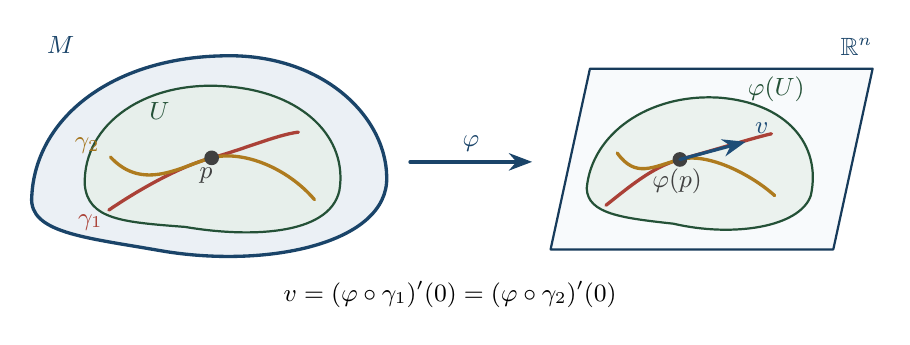
\begin{tikzpicture}[>=Stealth,scale=1.02,line cap=round,line join=round]
% Dwie różne krzywe, których pochodne w p po przejściu do współrzędnych są równe.
\filldraw[fill=manifoldblue!9,draw=manifoldblue!75!black,very thick]
 (-5.04,-.52) .. controls (-5.0,.46) and (-4.05,1.21) .. (-2.67,1.24)
 .. controls (-1.44,1.28) and (-.63,.5) .. (-.62,-.27)
 .. controls (-.6,-1.1) and (-2.13,-1.42) .. (-3.47,-1.18)
 .. controls (-4.39,-1.02) and (-5.07,-.96) .. cycle;
\filldraw[fill=manifoldgreen!12,draw=manifoldgreen!65!black,thick]
 (-4.38,-.36) .. controls (-4.4,.4) and (-3.61,.94) .. (-2.62,.86)
 .. controls (-1.65,.79) and (-1.1,.21) .. (-1.21,-.44)
 .. controls (-1.34,-1.01) and (-2.37,-1.02) .. (-3.13,-.89)
 .. controls (-3.91,-.83) and (-4.34,-.8) .. cycle;
\node[font=\small\bfseries,manifoldblue!75!black] at (-4.68,1.37) {$M$};
\node[font=\small,manifoldgreen!65!black] at (-3.45,.55) {$U$};
\draw[manifoldred,very thick]
 (-4.08,-.68) .. controls (-3.7,-.42) and (-3.18,-.13) .. (-2.8,-.03)
 .. controls (-2.42,.07) and (-1.98,.26) .. (-1.72,.29);
\draw[manifoldgold!85!black,very thick]
 (-4.06,-.02) .. controls (-3.65,-.46) and (-3.18,-.13) .. (-2.8,-.03)
 .. controls (-2.42,.07) and (-1.86,-.15) .. (-1.52,-.55);
\node[font=\small,manifoldred] at (-4.31,-.83) {$\gamma_1$};
\node[font=\small,manifoldgold!80!black] at (-4.35,.12) {$\gamma_2$};
\fill[black!75] (-2.8,-.03) circle (2.6pt)
 node[below,font=\small,xshift=-2pt] {$p$};
\draw[->,very thick,manifoldblue!75!black] (-.33,-.08)--(1.19,-.08)
 node[midway,above,font=\small] {$\varphi$};
% Rysunkowy fragment R^n oraz obraz U.
\filldraw[fill=manifoldblue!3,draw=manifoldblue!65!black,thick]
 (1.42,-1.17)--(4.94,-1.17)--(5.43,1.08)--(1.91,1.08)--cycle;
\filldraw[fill=manifoldgreen!10,draw=manifoldgreen!65!black,thick]
 (1.87,-.41) .. controls (1.93,.27) and (2.64,.77) .. (3.51,.72)
 .. controls (4.35,.66) and (4.8,.14) .. (4.66,-.5)
 .. controls (4.52,-.9) and (3.68,-1.02) .. (2.95,-.85)
 .. controls (2.32,-.78) and (1.88,-.73) .. cycle;
\draw[manifoldred,very thick]
 (2.11,-.62) .. controls (2.39,-.4) and (2.69,-.14) .. (3.03,-.05)
 .. controls (3.37,.04) and (3.91,.21) .. (4.17,.27);
\draw[manifoldgold!85!black,very thick]
 (2.25,.03) .. controls (2.48,-.29) and (2.69,-.14) .. (3.03,-.05)
 .. controls (3.37,.04) and (3.91,-.23) .. (4.21,-.5);
\fill[black!75] (3.03,-.05) circle (2.6pt)
 node[below,font=\small,xshift=-1pt] {$\varphi(p)$};
\draw[->,very thick,manifoldblue!85!black] (3.03,-.05)--(3.85,.17);
\node[font=\small,manifoldblue!85!black] at (4.05,.34) {$v$};
\node[font=\small,manifoldgreen!65!black] at (4.23,.82) {$\varphi(U)$};
\node[font=\small\bfseries,manifoldblue!75!black] at (5.23,1.35) {$\R^n$};
\node[font=\small] at (.17,-1.73)
 {$v=(\varphi\circ\gamma_1)'(0)=(\varphi\circ\gamma_2)'(0)$};
\end{tikzpicture}
\caption{Dwie krzywe w $M$ przechodzą przez $p$ i mają ten sam kierunek
styczny. W mapie $\varphi$ ich obrazy mają wspólną pochodną $v$ w $t=0$.}
\label{fig:krzywe-styczne-w-mapie}
\end{figure}

\begin{fakt}
Powyższy warunek nie zależy od wyboru mapy $(U,\varphi)$.
\end{fakt}
\begin{proof}
Jeśli $(V,\psi)$ jest inną mapą wokół $p$, to na wspólnej dziedzinie $\psi\circ\gamma_i=
(\psi\circ\varphi^{-1})\circ(\varphi\circ\gamma_i)$ blisko $t=0$, więc z reguły łańcucha
\[
(\psi\circ\gamma_i)'(0)=D(\psi\circ\varphi^{-1})(\varphi(p))\cdot(\varphi\circ\gamma_i)'(0),
\qquad i=1,2.
\]
Ponieważ $D(\psi\circ\varphi^{-1})(\varphi(p))$ jest tym samym przekształceniem liniowym
dla $i=1$ i $i=2$, równość $(\varphi\circ\gamma_1)'(0)=(\varphi\circ\gamma_2)'(0)$
implikuje $(\psi\circ\gamma_1)'(0)=(\psi\circ\gamma_2)'(0)$, i na odwrót (bo
$D(\psi\circ\varphi^{-1})(\varphi(p))$ jest odwracalne, jako różniczka dyfeomorfizmu).
\end{proof}

Relacja $\sim$ jest relacją równoważności na $\Gamma_p$ (natychmiast z definicji, poprzez
odpowiednie własności równości w $\R^n$). Definiujemy $T_p^AM:=\Gamma_p/\!\sim$.

Aby wyposażyć $T_p^AM$ w strukturę przestrzeni wektorowej, ustalmy mapę
$(U,\varphi)$ wokół $p$ i zdefiniujmy
\[
\Theta_\varphi:T_p^AM\longrightarrow\R^n,
\qquad
\Theta_\varphi([\gamma]):=(\varphi\circ\gamma)'(0).
\]
Odwzorowanie to jest dobrze określone i bijektywne. Różnowartościowość
wynika bezpośrednio z definicji relacji równoważności, natomiast
surjektywność z faktu, że dla dowolnego $v\in\R^n$ krzywa
\[
\gamma(t)=\varphi^{-1}(\varphi(p)+tv),
\]
określona dla dostatecznie małych $|t|$, spełnia
\[
\gamma(0)=p,
\qquad
(\varphi\circ\gamma)'(0)=v.
\]

Za pomocą bijekcji $\Theta_\varphi$ przenosimy strukturę przestrzeni
wektorowej z $\R^n$ na $T_p^AM$, definiując
\[
[\gamma]+[\eta]
:=
\Theta_\varphi^{-1}
\bigl(\Theta_\varphi([\gamma])+\Theta_\varphi([\eta])\bigr)
\]
oraz
\[
a[\gamma]
:=
\Theta_\varphi^{-1}
\bigl(a\,\Theta_\varphi([\gamma])\bigr),
\qquad a\in\R.
\]
W szczególności mnożenie przez skalar można reprezentować przez
reparametryzację krzywej:
\[
a[\gamma]=[t\mapsto\gamma(at)],
\]
ponieważ
\[
(\varphi\circ\gamma(at))'_{\,t=0}
=
a(\varphi\circ\gamma)'(0).
\]
W ten sposób $\Theta_\varphi$ jest, z definicji, izomorfizmem liniowym
$T_p^AM\cong\R^n$.

\begin{fakt}
Struktura liniowa na $T_p^AM$ nie zależy od wyboru mapy $\varphi$.
\end{fakt}
\begin{proof}
Niech $(V,\psi)$ będzie inną mapą wokół $p$, $L:=D(\psi\circ\varphi^{-1})(\varphi(p))
\colon\R^n\to\R^n$. Z rachunku w poprzednim Fakcie, dla dowolnej krzywej $\gamma\in\Gamma_p$,
$\Theta_\psi([\gamma])=L(\Theta_\varphi([\gamma]))$, czyli $\Theta_\psi=L\circ\Theta_\varphi$.
Ponieważ $L$ jest izomorfizmem \emph{liniowym} (jako różniczka dyfeomorfizmu w punkcie),
struktury liniowe przeniesione na $T_p^AM$ przez $\Theta_\varphi$ i przez $\Theta_\psi=
L\circ\Theta_\varphi$ pokrywają się: liniowość $L$ gwarantuje, że dla dowolnych $[\gamma_1],
[\gamma_2]\in T_p^AM$, $a,b\in\R$, kombinacja $a[\gamma_1]+b[\gamma_2]$ wyznaczona przez
$\Theta_\varphi$ pokrywa się z kombinacją wyznaczoną przez $\Theta_\psi$. To kluczowa
obserwacja: liniowość różniczki odwzorowania przejścia gwarantuje, że mimo iż
$\Theta_\varphi\neq\Theta_\psi$, wyznaczona przez nie struktura wektorowa na $T_p^AM$ jest
jedna i ta sama.
\end{proof}

\textbf{Definicja B (klasyczna, poprzez pary mapa-wektor).} Rozważmy zbiór trójek
$(U,\varphi,v)$, gdzie $(U,\varphi)$ jest mapą dopuszczalną wokół $p$, a $v\in\R^n$.
Mówimy, że $(U,\varphi,v)\sim(V,\psi,w)$, jeśli $w=D(\psi\circ\varphi^{-1})(\varphi(p))\,v$.

\begin{fakt}
Powyższa relacja jest relacją równoważności.
\end{fakt}
\begin{proof}
Zwrotność: dla $\psi=\varphi$, $D(\id)=\id$, więc $v=v$. Symetria: jeśli $w=D(\psi\varphi^{-1})
(\varphi(p))v$, to stosując regułę łańcucha do $\varphi\circ\psi^{-1}=(\psi\circ
\varphi^{-1})^{-1}$ w punkcie $\psi(p)$, $D(\varphi\psi^{-1})(\psi(p))=\big[D(\psi\varphi^{-1})
(\varphi(p))\big]^{-1}$, skąd $v=D(\varphi\psi^{-1})(\psi(p))w$. Przechodniość: jeśli
$w=D(\psi\varphi^{-1})(\varphi(p))v$ i $u=D(\eta\psi^{-1})(\psi(p))w$, to z reguły łańcucha
zastosowanej do $\eta\circ\varphi^{-1}=(\eta\circ\psi^{-1})\circ(\psi\circ\varphi^{-1})$ w
punkcie $\varphi(p)$,
\[
D(\eta\varphi^{-1})(\varphi(p))=D(\eta\psi^{-1})(\psi(p))\cdot D(\psi\varphi^{-1})(\varphi(p)),
\]
a więc $D(\eta\varphi^{-1})(\varphi(p))v=D(\eta\psi^{-1})(\psi(p))w=u$, czyli
$(U,\varphi,v)\sim(W,\eta,u)$.
\end{proof}

Definiujemy $T_p^BM$ jako zbiór klas równoważności
\[
[U,\varphi,v].
\]
Strukturę przestrzeni wektorowej wprowadzamy wzorem
\[
a[U,\varphi,v]+b[U,\varphi,v']
:=
[U,\varphi,av+bv'].
\]
Definicja ta jest dobrze określona, to znaczy wynik nie zależy od wyboru
reprezentantów klas. Istotnie, jeżeli przejdziemy do innej mapy
$(V,\psi)$ zawierającej punkt $p$, to wektory $v,v'\in\mathbb{R}^n$
przechodzą odpowiednio w
\[
D(\psi\circ\varphi^{-1})(\varphi(p))\,v
\qquad\text{oraz}\qquad
D(\psi\circ\varphi^{-1})(\varphi(p))\,v'.
\]
Z liniowości różniczki otrzymujemy
\[
D(\psi\circ\varphi^{-1})(\varphi(p))(av+bv')
=
a\,D(\psi\circ\varphi^{-1})(\varphi(p))v
+
b\,D(\psi\circ\varphi^{-1})(\varphi(p))v',
\]
a więc oba wybory reprezentantów prowadzą do tej samej klasy
równoważności.

Ustalmy teraz mapę $(U,\varphi)$ wokół punktu $p$. Definiujemy
odwzorowanie
\[
\Phi_\varphi\colon T_p^AM\longrightarrow T_p^BM,
\qquad
\Phi_\varphi([\gamma])
=
[U,\varphi,(\varphi\circ\gamma)'(0)].
\]
Odwzorowanie to jest dobrze określone, ponieważ jeżeli
$[\gamma]=[\eta]$ w $T_p^AM$, to z definicji relacji równoważności
krzywych mamy
\[
(\varphi\circ\gamma)'(0)
=
(\varphi\circ\eta)'(0),
\]
a zatem
\[
[U,\varphi,(\varphi\circ\gamma)'(0)]
=
[U,\varphi,(\varphi\circ\eta)'(0)].
\]

Żeby sprawdzić bijektywność, rozważmy odwzorowanie
\[
j_\varphi\colon\R^n\longrightarrow T_p^BM,
\qquad j_\varphi(v)=[U,\varphi,v].
\]
Jest ono liniowe na mocy definicji działań. Jest też
różnowartościowe: jeżeli $[U,\varphi,v]=[U,\varphi,w]$,
to relacja równoważności w tej samej mapie daje $v=w$.
Jest na, gdyż dla dowolnej klasy $[V,\psi,w]$ element
\[
v=D(\varphi\circ\psi^{-1})(\psi(p))w
\]
spełnia $[V,\psi,w]=[U,\varphi,v]$. Ponieważ
$\Theta_\varphi$ jest liniową bijekcją, mamy
$\Phi_\varphi=j_\varphi\circ\Theta_\varphi$,
a więc $\Phi_\varphi$ również jest liniową bijekcją.
Zmiana mapy nie zmienia tego odwzorowania: dla $(V,\psi)$
reguła łańcucha i definicja relacji równoważności dają
$j_\psi\circ\Theta_\psi=j_\varphi\circ\Theta_\varphi$.
Otrzymujemy zatem kanoniczne utożsamienie
\[
T_p^AM\cong T_p^BM.
\]
Od tej chwili obie te przestrzenie będziemy oznaczać wspólnym symbolem
\[
T_p^{\mathrm{geom}}M.
\]
\textbf{Definicja C (algebraiczna, poprzez derywacje).} Niech $C^\infty(M)$ oznacza
przestrzeń funkcji gładkich $M\to\R$. \emph{Derywacją w punkcie $p$} nazywamy funkcjonał
liniowy $v\colon C^\infty(M)\to\R$ spełniający regułę Leibniza:
\[
v(fg)=f(p)\,v(g)+g(p)\,v(f), \qquad f,g\in C^\infty(M).
\]
Zbiór wszystkich derywacji w $p$ oznaczamy $T_p^CM$ — jest to podprzestrzeń liniowa
przestrzeni funkcjonałów liniowych na $C^\infty(M)$ (suma i wielokrotność derywacji
spełnia regułę Leibniza — sprawdzenie bezpośrednie).

W dalszej części skonstruujemy kanoniczny izomorfizm
$T_p^{\mathrm{geom}}M\to T_p^CM$. Utożsamimy w ten sposób
wszystkie trzy definicje i otrzymamy bazę przestrzeni
stycznej złożoną z pochodnych cząstkowych.

\subsection*{Lemat Hadamarda}

Poniższy lemat analityczny jest podstawowym narzędziem technicznym tej sekcji.

\begin{lemat}[Lemat Hadamarda]\label{lem:hadamard}
Niech $\Omega\subseteq\R^n$ będzie zbiorem otwartym, gwiaździstym względem $0$ (tzn.\
$tx\in\Omega$ dla wszystkich $x\in\Omega$, $t\in[0,1]$), i niech $f\in C^\infty(\Omega)$.
Wówczas istnieją funkcje $g_1,\dots,g_n\in C^\infty(\Omega)$ takie, że
\[
f(x)=f(0)+\sum_{i=1}^nx^ig_i(x), \qquad x\in\Omega,
\]
oraz $g_i(0)=\dfrac{\partial f}{\partial x^i}(0)$ dla każdego $i$.
\end{lemat}

\begin{proof}
Dla ustalonego $x\in\Omega$, funkcja $t\mapsto f(tx)$ jest dobrze określona i gładka na
$[0,1]$ (bo $\Omega$ jest gwiaździsty względem $0$), więc z twierdzenia podstawowego
rachunku różniczkowego,
\[
f(x)-f(0)=\int_0^1\frac{d}{dt}f(tx)\,dt=\int_0^1\sum_{i=1}^n\frac{\partial f}{\partial x^i}
(tx)\,x^i\,dt=\sum_{i=1}^nx^i\underbrace{\int_0^1\frac{\partial f}{\partial x^i}(tx)\,dt}
_{=:g_i(x)}.
\]
Funkcje $g_i(x):=\int_0^1\frac{\partial f}{\partial x^i}(tx)\,dt$ są gładkie na $\Omega$
(różniczkowanie pod znakiem całki, dopuszczalne, gdyż funkcja podcałkowa zależy gładko od
$(t,x)$), oraz $g_i(0)=\int_0^1\frac{\partial f}{\partial x^i}(0)\,dt=\frac{\partial f}
{\partial x^i}(0)$, co kończy dowód.
\end{proof}

\subsection*{Od krzywych do derywacji}

Zdefiniujmy odwzorowanie $\Phi\colon T_p^AM\to T_p^CM$ wzorem
\[
\Phi([\gamma])(f):=(f\circ\gamma)'(0), \qquad f\in C^\infty(M).
\]

\begin{fakt}
$\Phi$ jest dobrze określone (niezależne od wyboru reprezentanta $\gamma$), a
$\Phi([\gamma])$ jest derywacją w $p$ dla każdego $[\gamma]\in T_p^AM$.
\end{fakt}
\begin{proof}
Niezależność od reprezentanta: jeśli $\gamma_1\sim\gamma_2$, to pisząc $f\circ\gamma_i=
(f\circ\varphi^{-1})\circ(\varphi\circ\gamma_i)$ dla mapy $(U,\varphi)$ wokół $p$,
\[
(f\circ\gamma_i)'(0)=D(f\circ\varphi^{-1})(\varphi(p))\cdot(\varphi\circ\gamma_i)'(0),
\]
a prawa strona zależy od $\gamma_i$ jedynie poprzez $(\varphi\circ\gamma_i)'(0)$, które z
założenia $\gamma_1\sim\gamma_2$ jest tym samym wektorem dla $i=1,2$. Liniowość
$\Phi([\gamma])$ względem $f$ wynika z liniowości pochodnej $(\cdot)'(0)$ oraz liniowości
$D(f\circ\varphi^{-1})$ względem $f$. Reguła Leibniza: $\big((fg)\circ\gamma\big)'(0)=
\big((f\circ\gamma)(g\circ\gamma)\big)'(0)=(f\circ\gamma)'(0)\,g(p)+f(p)\,(g\circ\gamma)'(0)
=\Phi([\gamma])(f)\,g(p)+f(p)\,\Phi([\gamma])(g)$, na mocy zwykłej reguły Leibniza dla
pochodnej iloczynu funkcji jednej zmiennej $t\mapsto f(\gamma(t))g(\gamma(t))$.
\end{proof}

Odwzorowanie
\[
\Phi\colon T_p^A M\to T_p^C M
\]
jest liniowe względem struktury wektorowej na $T_p^A M$ zdefiniowanej
za pomocą izomorfizmu
\[
\Theta_\varphi\colon T_p^A M\to\mathbb R^n.
\]
Istotnie, jeśli
\[
v=\Theta_\varphi([\gamma]),
\qquad
w=\Theta_\varphi([\eta]),
\]
to dla $a,b\in\mathbb R$ mamy
\[
\Theta_\varphi(a[\gamma]+b[\eta])=av+bw.
\]
Dla dowolnego $f\in C^\infty(M)$ otrzymujemy zatem
\begin{align*}
\Phi(a[\gamma]+b[\eta])(f)
&=
D(f\circ\varphi^{-1})(\varphi(p))(av+bw)\\
&=
a\,D(f\circ\varphi^{-1})(\varphi(p))(v)
+
b\,D(f\circ\varphi^{-1})(\varphi(p))(w)\\
&=
a\,\Phi([\gamma])(f)+b\,\Phi([\eta])(f).
\end{align*}
Stąd $\Phi$ jest odwzorowaniem liniowym.

Pokażemy teraz, że $\Phi$ jest izomorfizmem.
Kluczowym krokiem będzie zastosowanie Lematu Hadamarda, które
wyjaśni również, dlaczego pochodne cząstkowe
\[
\left.\frac{\partial}{\partial x^1}\right|_p,\ldots,
\left.\frac{\partial}{\partial x^n}\right|_p
\]
tworzą bazę $T_p^C M$.

Będziemy używać gładkiej \emph{funkcji odcinającej}
$\mu\colon\R^n\to[0,1]$ (ang.\ \emph{bump function}),
równej $1$ na $\overline{B(0,1)}$ i $0$ poza $B(0,2)$.
Zbudujmy ją jawnie. Niech $h(t)=e^{-1/t}$ dla $t>0$,
a $h(t)=0$ dla $t\leq0$. Wszystkie pochodne $h$ po
prawej stronie zera są sumami wyrazów postaci
$t^{-m}e^{-1/t}$, które dążą do zera przy $t\downarrow0$;
po lewej stronie wszystkie pochodne wynoszą zero.
Funkcja $h$ jest więc gładka także w zerze. Kładziemy
\[
 \theta(t):=\frac{h(t)}{h(t)+h(1-t)},\qquad
 \mu(x):=\theta\!\left(\frac{4-\|x\|^2}{3}\right).
\]
Mianownik $\theta$ nigdzie nie znika: dla $t\leq0$
dodatni jest $h(1-t)$, dla $t\geq1$ dodatni jest $h(t)$,
a pomiędzy nimi dodatnie są oba. Mamy $\theta(t)=0$
dla $t\leq0$ i $\theta(t)=1$ dla $t\geq1$.
Jeśli $\|x\|\leq1$, argument $\theta$ jest co najmniej $1$;
jeśli $\|x\|\geq2$, jest nie większy od zera.
Cała konstrukcja jest gładka, bo $\|x\|^2$ jest
wielomianem współrzędnych.


% ============================================================
% RYSUNEK 1
% U \subset W \subset M oraz mapa \varphi
% ============================================================

\begin{figure}[ht]
\centering

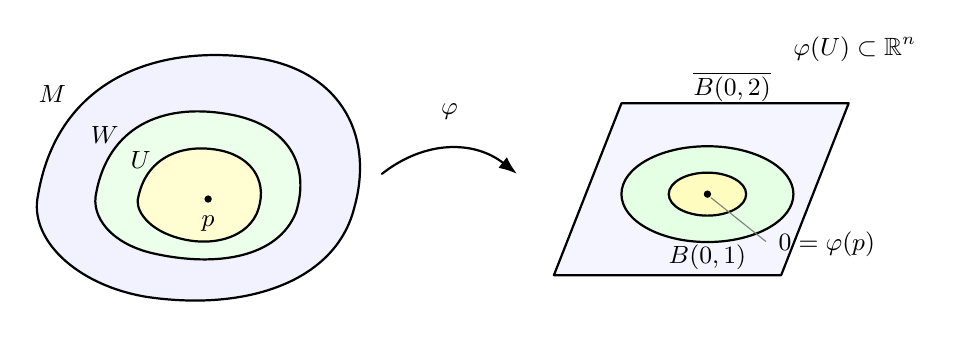
\begin{tikzpicture}[
    >=Latex,
    font=\small,
    line cap=round,
    line join=round,
    scale=0.78
]

% M
\draw[
    thick,
    fill=blue!5
]
    (-5.4,0.1)
    .. controls (-5.1,1.9) and (-3.6,2.55) .. (-1.95,2.35)
    .. controls (-0.55,2.2) and (0.10,1.15) .. (-0.25,-0.10)
    .. controls (-0.55,-1.30) and (-2.0,-1.80) .. (-3.65,-1.55)
    .. controls (-4.8,-1.35) and (-5.55,-0.60) .. (-5.4,0.1);

\node[anchor=west] at (-5.55,1.75)
    {$M$};

% W
\draw[
    thick,
    fill=green!8
]
    (-4.45,0.15)
    .. controls (-4.25,1.20) and (-3.40,1.60) .. (-2.35,1.43)
    .. controls (-1.35,1.28) and (-0.95,0.62) .. (-1.20,-0.18)
    .. controls (-1.50,-0.92) and (-2.50,-1.07) .. (-3.50,-0.85)
    .. controls (-4.20,-0.70) and (-4.55,-0.25) .. (-4.45,0.15);

\node[anchor=west] at (-4.70,1.08)
    {$W$};

% U
\draw[
    thick,
    fill=yellow!18
]
    (-3.76,0.10)
    .. controls (-3.62,0.72) and (-3.05,0.96) .. (-2.42,0.83)
    .. controls (-1.88,0.71) and (-1.64,0.28) .. (-1.84,-0.20)
    .. controls (-2.05,-0.65) and (-2.70,-0.76) .. (-3.25,-0.55)
    .. controls (-3.65,-0.40) and (-3.84,-0.10) .. (-3.76,0.10);

\node[anchor=west] at (-4.05,0.67)
    {$U$};

% Punkt p
\fill (-2.63,0.04) circle (1.7pt);

\node[below=5pt] at (-2.63,0.15)
    {$p$};

% Strzałka \varphi
\draw[->,thick]
    (0.20,0.45)
    .. controls (0.90,1.00) and (1.70,1.00) ..
    (2.40,0.45);

\node[above=5pt] at (1.30,0.95)
    {$\varphi$};

% Obraz mapy
\draw[
    thick,
    fill=blue!4
]
    (3.0,-1.2)
    --
    (4.1,1.6)
    --
    (7.8,1.6)
    --
    (6.7,-1.2)
    --
    cycle;

\node[above=7pt] at (7.90,1.80)
    {$\varphi(U)\subset\mathbb{R}^n$};

% \overline{B(0,2)}
\draw[
    thick,
    fill=green!10
]
    (5.50,0.12)
    ellipse (1.40 and 0.78);

\node[above=8pt] at (5.90,1.10)
    {$\overline{B(0,2)}$};

% B(0,1)
\draw[
    thick,
    fill=yellow!25
]
    (5.50,0.12)
    ellipse (0.63 and 0.35);

\node[below=7pt] at (5.50,-0.23)
    {$B(0,1)$};

% 0 = \varphi(p)
\fill (5.50,0.12) circle (1.7pt);

\draw[thin,gray] (5.56,0.06) -- (6.45,-0.65);
\node[anchor=west] at (6.50,-0.70)
    {$0=\varphi(p)$};

\end{tikzpicture}

\caption{
Wybór mapy $(U,\varphi)$ wokół punktu $p$:
$U\subseteq W$, $\varphi(p)=0$ oraz
$\overline{B(0,2)}\subseteq\varphi(U)$.
}
\label{fig:kapelusz-mapa}

\end{figure}


% ============================================================
% RYSUNEK 2
% Wykres funkcji kapelusz
% ============================================================

\begin{figure}[ht]
\centering

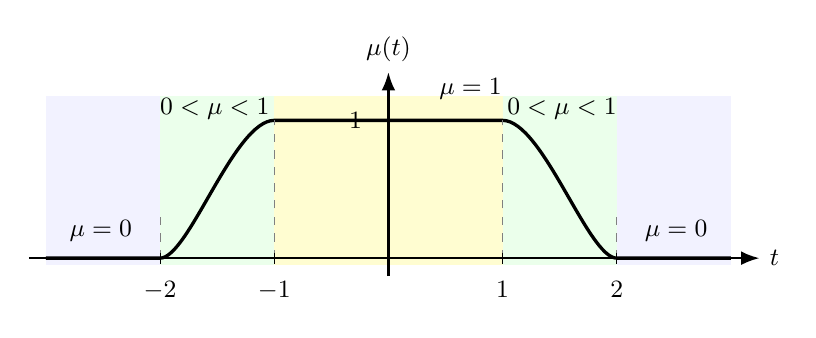
\begin{tikzpicture}[
    >=Latex,
    font=\small,
    x=1.45cm,
    y=1.75cm
]

% Delikatne kolorowe obszary
\fill[blue!5]
    (-3,-0.05)
    rectangle
    (-2,1.18);

\fill[green!8]
    (-2,-0.05)
    rectangle
    (-1,1.18);

\fill[yellow!18]
    (-1,-0.05)
    rectangle
    (1,1.18);

\fill[green!8]
    (1,-0.05)
    rectangle
    (2,1.18);

\fill[blue!5]
    (2,-0.05)
    rectangle
    (3,1.18);

% Oś pozioma
\draw[->,thick]
    (-3.15,0)
    --
    (3.25,0)
    node[right] {$t$};

% Oś pionowa
\draw[->,thick]
    (0,-0.13)
    --
    (0,1.35)
    node[above] {$\mu(t)$};

% Wykres funkcji kapelusz
\draw[very thick]
    (-3,0)
    --
    (-2,0)
    .. controls (-1.75,0) and (-1.35,1) ..
    (-1,1)
    --
    (1,1)
    .. controls (1.35,1) and (1.75,0) ..
    (2,0)
    --
    (3,0);

% Linie pomocnicze
\draw[dashed,gray]
    (-1,0) -- (-1,1);

\draw[dashed,gray]
    (1,0) -- (1,1);

\draw[dashed,gray]
    (-2,0) -- (-2,0.36);

\draw[dashed,gray]
    (2,0) -- (2,0.36);

% Znaczniki na osi
\draw
    (-2,0.04) -- (-2,-0.04);
\node[below=5pt] at (-2,0)
    {$-2$};

\draw
    (-1,0.04) -- (-1,-0.04);
\node[below=5pt] at (-1,0)
    {$-1$};

\draw
    (1,0.04) -- (1,-0.04);
\node[below=5pt] at (1,0)
    {$1$};

\draw
    (2,0.04) -- (2,-0.04);
\node[below=5pt] at (2,0)
    {$2$};

% Poziom 1
\draw
    (-0.04,1) -- (0.04,1);

\node[left=6pt] at (0,1)
    {$1$};

% Opisy — odsunięte od wykresu
\node[above=4pt] at (0.72,1)
    {$\mu=1$};

\node at (-1.52,1.08)
    {$0<\mu<1$};

\node at (1.52,1.08)
    {$0<\mu<1$};

\node at (-2.52,0.20)
    {$\mu=0$};

\node at (2.52,0.20)
    {$\mu=0$};

\end{tikzpicture}

\caption{
Jednowymiarowy przekrój funkcji odcinającej $\mu$.
Funkcja jest równa $1$ dla $|t|\leq1$,
płynnie maleje dla $1<|t|<2$
i znika dla $|t|\geq2$.
}
\label{fig:kapelusz-wykres}

\end{figure}




\begin{lemat}[Lokalność derywacji]\label{lem:lokalnosc}
Niech $v\in T_p^CM$ będzie derywacją w $p$. Jeśli $h\in C^\infty(M)$ znika na pewnym
otoczeniu punktu $p$, to $v(h)=0$. W szczególności, jeśli $f,g\in C^\infty(M)$ pokrywają
się na pewnym otoczeniu $p$, to $v(f)=v(g)$; wartość $v(f)$ zależy więc jedynie od
zachowania $f$ w dowolnie małym otoczeniu $p$.
\end{lemat}
\begin{proof}
Z reguły Leibniza zastosowanej do $f=g=\mathbf1$ (funkcji stałej równej $1$),
$v(\mathbf1)=v(\mathbf1\cdot\mathbf1)=2v(\mathbf1)$, skąd $v(\mathbf1)=0$; z liniowości,
$v(c)=0$ dla każdej funkcji stałej $c$.

Niech $h\equiv0$ na otoczeniu otwartym $W\ni p$. Wybierzmy mapę $(U,\varphi)$ wokół $p$ z
$U\subseteq W$, $\varphi(p)=0$, oraz (po przeskalowaniu)
$\overline{B(0,2)}\subseteq\varphi(U)$.
Zdefiniujmy $\tilde\mu\colon M\to\R$: $\tilde\mu(q):=\mu(\varphi(q))$ dla $q\in U$, oraz
$\tilde\mu(q):=0$ dla $q\notin U$. Nośnik jest zawarty w zwartym
zbiorze $K=\varphi^{-1}(\overline{B(0,2)})\subset U$.
Ponieważ $M$ jest Hausdorffa, $K$ jest domknięty w $M$.
Na otwartym pokryciu $U, M\setminus K$ obie gładkie definicje
pokrywają się, więc $\tilde\mu\in C^\infty(M)$, równa $1$ na otoczeniu $p$ i znikająca poza
$U\subseteq W$. Wówczas $\tilde\mu\cdot h\equiv0$ na całym $M$, więc $v(\tilde\mu h)=0$.
Z reguły Leibniza, $0=v(\tilde\mu h)=\tilde\mu(p)v(h)+h(p)v(\tilde\mu)=v(h)$ (bo
$\tilde\mu(p)=1$, $h(p)=0$). Zatem $v(h)=0$. Ostatnia część lematu wynika z zastosowania
powyższego do $h:=f-g$.
\end{proof}

\begin{twierdzenie}\label{tw:baza-styczna}
Niech $(U,\varphi)$ będzie mapą dopuszczalną wokół $p$,
$\varphi=(x^1,\dots,x^n)$,
gdzie $x^i=\pi_i\circ\varphi\colon U\to\R$ są funkcjami współrzędnymi,
czyli dla każdego $q\in U$ zachodzi
$\varphi(q)=\bigl(x^1(q),\dots,x^n(q)\bigr)$,
oraz załóżmy, że $\varphi(p)=0$. Wówczas:
\begin{enumerate}[label=(\alph*)]
\item Odwzorowanie $\Phi\colon T_p^AM\to T_p^CM$ jest izomorfizmem liniowym.
\item Elementy $\frac{\partial}{\partial x^1}\big|_p,\dots,\frac{\partial}{\partial x^n}
\big|_p\in T_p^CM$, zdefiniowane przez $\frac{\partial}{\partial x^i}\big|_p(f):=
\frac{\partial(f\circ\varphi^{-1})}{\partial x^i}(\varphi(p))$, stanowią bazę $T_p^CM$.
W szczególności $\dim T_pM=n$.
\end{enumerate}
\end{twierdzenie}

\begin{proof}
\emph{(a), injektywność.} Załóżmy $\Phi([\gamma])=0$, tzn.\ $(f\circ\gamma)'(0)=0$ dla
wszystkich $f\in C^\infty(M)$. Wybierzmy funkcję odcinającą
$\tilde\mu$ o zwartym nośniku zawartym w $U$, równą $1$ blisko $p$,
jak w dowodzie Lematu~\ref{lem:lokalnosc}.
Dla $i=1,\dots,n$ niech $\tilde x^i:=\tilde\mu\,x^i
=\tilde\mu\,\varphi^i$ na $U$ (rozszerzone przez $0$ poza $U$) —
funkcja gładka na $M$, pokrywająca się z $\varphi^i$ na otoczeniu $p$. Z założenia,
$0=\Phi([\gamma])(\tilde x^i)=(\tilde x^i\circ\gamma)'(0)$; blisko $t=0$, $\gamma(t)\in U$
i tam $\tilde x^i\circ\gamma=\varphi^i\circ\gamma$, więc $(\varphi^i\circ\gamma)'(0)=0$ dla
każdego $i$, czyli $(\varphi\circ\gamma)'(0)=0\in\R^n$. Oznacza to $\gamma\sim
\gamma_{\text{stała}}$ (gdzie $\gamma_{\text{stała}}(t)\equiv p$), czyli $[\gamma]=0$ w
$T_p^AM$. Zatem $\ker\Phi=\{0\}$.

\emph{(a), surjektywność — Lemat Hadamarda.} Niech $v\in T_p^CM$. Bez straty ogólności
$\varphi(U)$ jest kulą (gwiaździstą względem $0$). Niech $\tilde f:=f\circ\varphi^{-1}\in
C^\infty(\varphi(U))$; z Lematu~\ref{lem:hadamard} istnieją $g_1,\dots,g_n$ z
\[
\tilde f(x)=\tilde f(0)+\sum_ix^ig_i(x), \qquad g_i(0)=\frac{\partial\tilde f}{\partial x^i}
(0)=\frac{\partial}{\partial x^i}\Big|_p(f).
\]
Podstawiając $x=\varphi(q)$: $f(q)=f(p)+\sum_i\varphi^i(q)\,g_i(\varphi(q))$ dla $q$
blisko $p$. Niech $\widetilde{\varphi^i}$, $\tilde g_i$ oznaczają (jak wyżej) rozszerzenia
$\varphi^i$ oraz $g_i\circ\varphi$ do funkcji gładkich na $M$, pokrywające się z
oryginałami na otoczeniu $p$. Funkcja $F:=f(p)\cdot\mathbf1+\sum_i\widetilde{\varphi^i}\,
\tilde g_i$ pokrywa się z $f$ na otoczeniu $p$, więc $v(f)=v(F)$ (Lemat~\ref{lem:lokalnosc}).
Z liniowości $v$, reguły Leibniza (korzystając z $\widetilde{\varphi^i}(p)=0$,
$v(\mathbf1)=0$):
\[
v(f)=v(F)=\sum_i\Big(\widetilde{\varphi^i}(p)\,v(\tilde g_i)+\tilde g_i(p)\,v
(\widetilde{\varphi^i})\Big)=\sum_ig_i(0)\,v(\widetilde{\varphi^i})=\sum_{i=1}^n
v(\widetilde{\varphi^i})\cdot\frac{\partial}{\partial x^i}\Big|_p(f).
\]
Kładąc $c_i:=v(\widetilde{\varphi^i})\in\R$, mamy $v=\sum_ic_i\,\frac{\partial}{\partial
x^i}\big|_p$ jako funkcjonały. Niech $\gamma(t):=\varphi^{-1}(t\cdot(c_1,\dots,c_n))$; wtedy
$\Phi([\gamma])(f)=(f\circ\gamma)'(0)=D(f\circ\varphi^{-1})(0)\cdot(c_1,\dots,c_n)=
\sum_ic_i\frac{\partial}{\partial x^i}\big|_p(f)=v(f)$ dla każdego $f$, czyli
$\Phi([\gamma])=v$. To dowodzi surjektywności, a wraz z liniowością i injektywnością —
części (a).

\emph{(b).} Powyższy rachunek pokazał, że każdy $v\in T_p^CM$ jest kombinacją liniową
$\sum_ic_i\frac{\partial}{\partial x^i}\big|_p$ — więc baza ta rozpina $T_p^CM$. Niezależność
liniowa: załóżmy $\sum_ic_i\frac{\partial}{\partial x^i}\big|_p=0$. Stosując obie strony
do $\widetilde{\varphi^j}$ i korzystając z $\frac{\partial}{\partial x^i}\big|_p
(\widetilde{\varphi^j})=\frac{\partial x^j}{\partial x^i}(0)=\delta_i^j$, otrzymujemy
$0=\sum_ic_i\delta_i^j=c_j$ dla każdego $j$. Zatem $\{\partial/\partial x^i|_p\}$ jest
bazą $T_p^CM$; w szczególności $\dim T_p^CM=n$.
\end{proof}

\begin{wniosek}
Definicje A, B i C przestrzeni stycznej są kanonicznie izomorficzne. Piszemy odtąd po
prostu $T_pM$ i mówimy o \emph{przestrzeni stycznej do $M$ w punkcie $p$} — jest to
$n$-wymiarowa przestrzeń wektorowa. W mapie $(U,\varphi)$, gdzie $\varphi=(x^1,\dots,x^n)$,
jej \emph{bazą współrzędnościową} są wektory
\[
\left.\frac{\partial}{\partial x^1}\right|_p,\ \dots,\
\left.\frac{\partial}{\partial x^n}\right|_p.
\]
\end{wniosek}

\begin{figure}[ht]
\centering
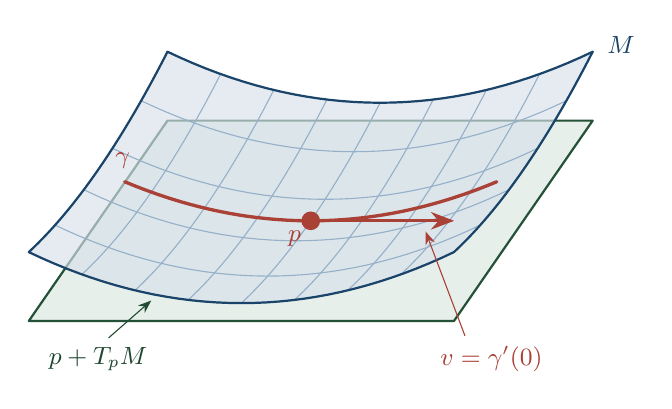
\begin{tikzpicture}[>=Stealth,scale=1.35,line cap=round,line join=round]
% S(u,v)=(u,v,.12u^2+.08v^2), rzut (x,y,z)->(x+.45y,.65y+z).
% Brzeg wypełnienia, siatka i krzywa używają tej samej parametryzacji.
\filldraw[fill=manifoldgreen!12,draw=manifoldgreen!65!black,thick]
 (-2.6525,-.9425)--(1.3475,-.9425)--(2.6525,.9425)--(-1.3475,.9425)--cycle;
\path[fill=manifoldblue!18,opacity=.65]
 (-2.65250,-0.29430)
  --(-2.48583,-0.37097)
  --(-2.31917,-0.44097)
  --(-2.15250,-0.50430)
  --(-1.98583,-0.56097)
  --(-1.81917,-0.61097)
  --(-1.65250,-0.65430)
  --(-1.48583,-0.69097)
  --(-1.31917,-0.72097)
  --(-1.15250,-0.74430)
  --(-0.98583,-0.76097)
  --(-0.81917,-0.77097)
  --(-0.65250,-0.77430)
  --(-0.48583,-0.77097)
  --(-0.31917,-0.76097)
  --(-0.15250,-0.74430)
  --(0.01417,-0.72097)
  --(0.18083,-0.69097)
  --(0.34750,-0.65430)
  --(0.51417,-0.61097)
  --(0.68083,-0.56097)
  --(0.84750,-0.50430)
  --(1.01417,-0.44097)
  --(1.18083,-0.37097)
  --(1.34750,-0.29430)
  --(1.40187,-0.24262)
  --(1.45625,-0.18861)
  --(1.51063,-0.13226)
  --(1.56500,-0.07358)
  --(1.61938,-0.01256)
  --(1.67375,0.05080)
  --(1.72812,0.11649)
  --(1.78250,0.18452)
  --(1.83688,0.25489)
  --(1.89125,0.32759)
  --(1.94562,0.40263)
  --(2.00000,0.48000)
  --(2.05437,0.55971)
  --(2.10875,0.64176)
  --(2.16312,0.72614)
  --(2.21750,0.81286)
  --(2.27188,0.90191)
  --(2.32625,0.99330)
  --(2.38063,1.08703)
  --(2.43500,1.18309)
  --(2.48937,1.28149)
  --(2.54375,1.38222)
  --(2.59813,1.48529)
  --(2.65250,1.59070)
  --(2.48583,1.51403)
  --(2.31917,1.44403)
  --(2.15250,1.38070)
  --(1.98583,1.32403)
  --(1.81917,1.27403)
  --(1.65250,1.23070)
  --(1.48583,1.19403)
  --(1.31917,1.16403)
  --(1.15250,1.14070)
  --(0.98583,1.12403)
  --(0.81917,1.11403)
  --(0.65250,1.11070)
  --(0.48583,1.11403)
  --(0.31917,1.12403)
  --(0.15250,1.14070)
  --(-0.01417,1.16403)
  --(-0.18083,1.19403)
  --(-0.34750,1.23070)
  --(-0.51417,1.27403)
  --(-0.68083,1.32403)
  --(-0.84750,1.38070)
  --(-1.01417,1.44403)
  --(-1.18083,1.51403)
  --(-1.34750,1.59070)
  --(-1.40187,1.48529)
  --(-1.45625,1.38222)
  --(-1.51063,1.28149)
  --(-1.56500,1.18309)
  --(-1.61938,1.08703)
  --(-1.67375,0.99330)
  --(-1.72812,0.90191)
  --(-1.78250,0.81286)
  --(-1.83688,0.72614)
  --(-1.89125,0.64176)
  --(-1.94562,0.55971)
  --(-2.00000,0.48000)
  --(-2.05437,0.40263)
  --(-2.10875,0.32759)
  --(-2.16312,0.25489)
  --(-2.21750,0.18452)
  --(-2.27188,0.11649)
  --(-2.32625,0.05080)
  --(-2.38063,-0.01256)
  --(-2.43500,-0.07358)
  --(-2.48937,-0.13226)
  --(-2.54375,-0.18861)
  --(-2.59813,-0.24262) --cycle;
\foreach \vv in {-1.45,-.9,-.3,.3,.9,1.45}{
 \draw[manifoldblue!48,thin] plot[domain=-2:2,samples=35]
  ({\x+.45*\vv},{.65*\vv+.12*\x*\x+.08*\vv*\vv});}
\foreach \uu in {-2,-1.5,-1,-.5,0,.5,1,1.5,2}{
 \draw[manifoldblue!48,thin] plot[domain=-1.45:1.45,samples=30]
  ({\uu+.45*\x},{.65*\x+.12*\uu*\uu+.08*\x*\x});}
\foreach \vv in {-1.45,1.45}{
 \draw[manifoldblue!75!black,thick] plot[domain=-2:2,samples=35]
  ({\x+.45*\vv},{.65*\vv+.12*\x*\x+.08*\vv*\vv});}
\foreach \uu in {-2,2}{
 \draw[manifoldblue!75!black,thick] plot[domain=-1.45:1.45,samples=30]
  ({\uu+.45*\x},{.65*\x+.12*\uu*\uu+.08*\x*\x});}
\draw[manifoldred,very thick] plot[domain=-1.75:1.75,samples=40]
 ({\x},{.12*\x*\x});
\fill[manifoldred] (0,0) circle (2.5pt) node[below left,font=\small] {$p$};
\draw[->,very thick,manifoldred] (0,0)--(1.35,0);
\node[font=\small,manifoldred] at (-1.77,.57) {$\gamma$};
\node[font=\small\bfseries,manifoldblue!75!black] at (2.92,1.65) {$M$};
\node[font=\small,manifoldgreen!55!black] at (-2.0,-1.30) {$p+T_pM$};
\draw[->,manifoldgreen!60!black,thin] (-1.9,-1.10)--(-1.5,-.75);
\node[font=\small,manifoldred] at (1.7,-1.30) {$v=\gamma'(0)$};
\draw[->,manifoldred,thin] (1.45,-1.08)--(1.08,-.10);
\end{tikzpicture}
\caption{Przestrzeń styczna: zielony równoległobok przedstawia afiniczną
płaszczyznę $p+T_pM$ przy zanurzonej powierzchni $M$. Czerwona krzywa
$\gamma$ leży na $M$, a wektor $v=\gamma'(0)$ leży w płaszczyźnie stycznej.
Siatka powierzchni odchyla się od tej płaszczyzny poza punktem $p$.}
\label{fig:tangent}
\end{figure}


\subsection*{Zmiana współrzędnych wektora stycznego}

\begin{fakt}
Niech $(U,\varphi)$ i $(V,\psi)$ będą mapami wokół $p\in M$, a
$[\gamma]\in T_pM$, gdzie
\[
\gamma:(-\varepsilon,\varepsilon)\to M,
\qquad
\gamma(0)=p.
\]
Współrzędne wektora $[\gamma]$ w mapie $\varphi$ są dane przez
\[
[\gamma]_{\varphi}:=(\varphi\circ\gamma)'(0)\in\R^n,
\]
a w mapie $\psi$ przez
\[
[\gamma]_{\psi}:=(\psi\circ\gamma)'(0).
\]
Wtedy
\[
\boxed{
[\gamma]_{\psi}
=
D(\psi\circ\varphi^{-1})(\varphi(p))\,[\gamma]_{\varphi}.
}
\]
\end{fakt}

\begin{proof}
Ponieważ
\[
\psi\circ\gamma
=
(\psi\circ\varphi^{-1})\circ(\varphi\circ\gamma),
\]
z reguły łańcuchowej otrzymujemy
\[
(\psi\circ\gamma)'(0)
=
D(\psi\circ\varphi^{-1})(\varphi(p))
\,(\varphi\circ\gamma)'(0),
\]
czyli dokładnie
\[
[\gamma]_{\psi}
=
D(\psi\circ\varphi^{-1})(\varphi(p))\,[\gamma]_{\varphi}.
\]
\end{proof}


\begin{przyklad}[Zmiana współrzędnych wektora stycznego na $\mathbb{RP}^2$]
\label{prz:RP2-styczna-1}
Wróćmy do map z przykładu~\ref{prz:RP2-przejscie-1}:
punkt $[1:u:v]$, gdzie $u\ne0$, ma w drugiej mapie współrzędne
$(a,b)=(1/u,v/u)$. Zastosujemy do tego przejścia właśnie udowodnioną
regułę zmiany współrzędnych wektora stycznego.

Odwzorowanie $\varphi_1\circ\varphi_0^{-1}$ opisuje zmianę
\emph{współrzędnych punktów} rozmaitości. Jego różniczka opisuje natomiast
odpowiadającą jej zmianę \emph{współrzędnych wektorów stycznych}.

Niech $p\in U_0\cap U_1$ oraz
\[
\varphi_0(p)=(u,v).
\]
Mapy $\varphi_0$ i $\varphi_1$ wyznaczają dwie bazy przestrzeni stycznej
$T_p\mathbb{RP}^2$:
\[
\left\{
\left.\frac{\partial}{\partial u}\right|_p,
\left.\frac{\partial}{\partial v}\right|_p
\right\},
\qquad
\left\{
\left.\frac{\partial}{\partial a}\right|_p,
\left.\frac{\partial}{\partial b}\right|_p
\right\}.
\]
Jeżeli wektor $X\in T_p\mathbb{RP}^2$ ma w bazie indukowanej przez
$\varphi_0$ współrzędne
\[
X
=
\dot u\left.\frac{\partial}{\partial u}\right|_p
+
\dot v\left.\frac{\partial}{\partial v}\right|_p,
\]
to jego współrzędne w bazie indukowanej przez $\varphi_1$ otrzymujemy,
stosując różniczkę odwzorowania przejścia:
\[
\begin{pmatrix}
\dot a\\[1mm]
\dot b
\end{pmatrix}
=
D(\varphi_1\circ\varphi_0^{-1})(u,v)
\begin{pmatrix}
\dot u\\[1mm]
\dot v
\end{pmatrix}.
\]
A zatem
\[
\dot a=-\frac{\dot u}{u^2},
\qquad
\dot b
=
-\frac{v\dot u}{u^2}
+
\frac{\dot v}{u}.
\]
Ten sam wektor styczny możemy więc zapisać jako
\[
X
=
\dot u\left.\frac{\partial}{\partial u}\right|_p
+
\dot v\left.\frac{\partial}{\partial v}\right|_p
=
\dot a\left.\frac{\partial}{\partial a}\right|_p
+
\dot b\left.\frac{\partial}{\partial b}\right|_p.
\]

Innymi słowy, odwzorowanie przejścia
$\varphi_1\circ\varphi_0^{-1}$ zmienia współrzędne punktu na rozmaitości,
natomiast jego różniczka
\[
d(\varphi_1\circ\varphi_0^{-1})_{\varphi_0(p)}
\]
zmienia reprezentację współrzędnościową tego samego wektora
$X\in T_p\mathbb{RP}^2$ względem baz przestrzeni stycznej indukowanych
przez obie mapy.
\end{przyklad}

\subsection*{Przestrzeń styczna w punkcie brzegu}

Niech teraz $p\in\partial M$. \emph{Kiełek}\index{kielek funkcji@Kiełek funkcji} funkcji gładkiej w $p$
to jej klasa względem równości w pewnym otoczeniu punktu $p$
otwartym w $M$;
funkcje są tu gładkie w sensie przedłużalności z półprzestrzeni.
Ich algebra to $C^\infty_p(M)$. Definiujemy $T_pM$ jako przestrzeń
$\R$-liniowych derywacji $D:C^\infty_p(M)\to\R$ spełniających
\[
 D(fg)=f(p)D(g)+g(p)D(f).
\]
Wartość kiełka w $p$ jest dobrze określona. To lokalna wersja
Definicji C, która nie wymaga krzywej przechodzącej przez $p$
w obu kierunkach czasu.

Użycie kiełków jest tutaj istotne. Gładkie przedłużenie funkcji
$f$ poza brzeg, do otoczenia $\varphi(p)$ w $\R^n$, nie jest
jednoznaczne i stanowi jedynie pomocnicze narzędzie służące do
zdefiniowania gładkości. Przestrzeń styczna powinna natomiast zależeć
wyłącznie od lokalnego zachowania funkcji na samej rozmaitości $M$,
a nie od arbitralnego wyboru jej wartości poza $M$.

Dokładniej, dwa różne gładkie przedłużenia
$\widetilde f_1,\widetilde f_2$ mogą być różnymi funkcjami na
otoczeniu $\varphi(p)$ w $\R^n$, mimo że ich ograniczenia do
$\mathbb H^n$ wyznaczają tę samą funkcję na $M$. Nie chcemy więc
traktować samych przedłużeń jako obiektów, na których działa derywacja.
Obiektem właściwym jest kiełek funkcji na $M$, natomiast przedłużenie
wybieramy dopiero wtedy, gdy chcemy wykonać rachunek we współrzędnych.

Co więcej, derywacja w punkcie $p$ jest obiektem lokalnym: jej wartość
na funkcji zależy jedynie od zachowania tej funkcji w dowolnie małym
otoczeniu $p$. Dlatego naturalną dziedziną derywacji jest algebra
kiełków $C^\infty_p(M)$.

\begin{stwierdzenie}[Pełny wymiar przestrzeni stycznej przy brzegu]
\label{prop:styczna-brzeg-1}
W mapie półprzestrzennej $\varphi$ z $\varphi(p)=0$ każda taka
derywacja ma jednoznaczną postać
\[
D(f)=\sum_{i=1}^n v^i\partial_i\widetilde f(0),
\qquad v\in\R^n,
\]
gdzie $\widetilde f$ jest dowolnym gładkim przedłużeniem
$f\circ\varphi^{-1}$ na otoczenie zera w $\R^n$.
Wzór nie zależy od wyboru przedłużenia. Przy zmianie mapy współrzędne
$v$ zmieniają się przez odwracalną macierz Jacobiego przejścia.
W szczególności $\dim T_pM=n$, a inkluzja brzegu identyfikuje
$T_p\partial M$ z podprzestrzenią $v^n=0$.
\end{stwierdzenie}

\begin{proof}
Najpierw sprawdźmy, że prawa strona wzoru nie zależy od wyboru
przedłużenia $\widetilde f$. Jeżeli $\widetilde f_1$ i
$\widetilde f_2$ są dwoma gładkimi przedłużeniami reprezentującymi
ten sam kiełek funkcji $f\circ\varphi^{-1}$, to ich różnica znika
na pewnej małej półkuli
\[
B_\varepsilon(0)\cap\mathbb H^n.
\]
Na jej części wewnętrznej, gdzie $x^n>0$, znikają więc wszystkie
pierwsze pochodne tej różnicy, a przez ciągłość znikają one również
w punkcie $0$. W konsekwencji
\[
\partial_i\widetilde f_1(0)
=
\partial_i\widetilde f_2(0),
\qquad i=1,\ldots,n.
\]
Zatem dla każdego $v\in\R^n$ wzór
\[
D_v(f):=\sum_{i=1}^n v^i\partial_i\widetilde f(0)
\]
jest dobrze określony na kiełkach. Jest on liniowy i spełnia regułę
Leibniza, a więc definiuje derywację w punkcie $p$.

Pokażmy teraz odwrotnie, że każda derywacja $D$ ma taką postać.
Najpierw
\[
D(1)=D(1\cdot1)=2D(1),
\]
zatem $D(1)=0$, a przez liniowość $D$ znika na wszystkich funkcjach
stałych.

Wybierzmy gładkie przedłużenie $\widetilde f$ funkcji
$f\circ\varphi^{-1}$ na małą kulę wokół zera. Lemat Hadamarda daje
\[
\widetilde f(x)
=
\widetilde f(0)+\sum_{i=1}^n x^i g_i(x),
\qquad
g_i(0)=\partial_i\widetilde f(0).
\]
Po ograniczeniu do półkuli otrzymujemy równość funkcji
reprezentujących kiełki w $0$, a więc
\[
[f\circ\varphi^{-1}]_0
=
\widetilde f(0)[1]_0
+
\sum_{i=1}^n [x^i]_0[g_i]_0.
\]

Niech również $x^i=\pi_i\circ\varphi$ oznacza $i$-tą funkcję
współrzędną na $U$. Stosując derywację $D$ do powyższej równości
kiełków oraz korzystając z $D(1)=0$ i $x^i(p)=0$, otrzymujemy
\[
D(f)
=
\sum_{i=1}^n D(x^i)\,g_i(0).
\]
Ponieważ
\[
g_i(0)=\partial_i\widetilde f(0),
\]
mamy
\[
D(f)
=
\sum_{i=1}^n D(x^i)\,\partial_i\widetilde f(0).
\]
Definiując
\[
v^i:=D(x^i),
\qquad i=1,\ldots,n,
\]
otrzymujemy żądaną postać
\[
D(f)
=
\sum_{i=1}^n v^i\partial_i\widetilde f(0).
\]

Współczynniki $v^i$ są jednoznaczne. Istotnie, stosując powyższy
wzór do funkcji współrzędnej $x^j$, otrzymujemy
\[
D(x^j)
=
\sum_{i=1}^n v^i\partial_i x^j(0)
=
\sum_{i=1}^n v^i\delta_i^j
=
v^j.
\]

Rozważmy dwie mapy półprzestrzenne $\varphi$ i $\psi$.
Odwzorowania przejścia
\[
\varphi\circ\psi^{-1}
\qquad\text{oraz}\qquad
\psi\circ\varphi^{-1}
\]
są wzajemnie odwrotne. Na punktach odpowiadających wnętrzu $M$ mamy zatem
\[
(\psi\circ\varphi^{-1})\circ(\varphi\circ\psi^{-1})
=\operatorname{id}
\]
oraz
\[
(\varphi\circ\psi^{-1})\circ(\psi\circ\varphi^{-1})
=\operatorname{id}.
\]
Stosując regułę łańcuchową do gładkich przedłużeń odwzorowań
przejścia, otrzymujemy na punktach wnętrza
\[
D(\psi\circ\varphi^{-1})(\varphi(q))\,
D(\varphi\circ\psi^{-1})(\psi(q))
=I.
\]
Przechodząc z $q\in\operatorname{int}M$ do $p\in\partial M$
i korzystając z ciągłości różniczek, otrzymujemy
\[
D(\psi\circ\varphi^{-1})(\varphi(p))\,
D(\varphi\circ\psi^{-1})(\psi(p))
=I.
\]
Analogicznie iloczyn w odwrotnej kolejności jest równy $I$.
Zatem macierze Jacobiego odwzorowań przejścia w punkcie brzegowym
są wzajemnie odwrotne.

Wreszcie ograniczenie mapy $\varphi$ do brzegu ma współrzędne
$(x^1,\ldots,x^{n-1})$. Różniczka inkluzji
$\partial M\hookrightarrow M$ dodaje zerową ostatnią współrzędną,
a zatem identyfikuje $T_p\partial M$ z podprzestrzenią
\[
\{v\in\R^n:v^n=0\}\subset T_pM.
\]
\end{proof}

Można też użyć derywacji funkcji globalnych: lokalność dowodzimy
jak wcześniej, a każdy kiełek ma globalnego reprezentanta po
pomnożeniu przez funkcję odcinającą równą $1$ blisko $p$,
o nośniku zawartym w dziedzinie reprezentanta, i przedłużeniu przez zero.
Taką funkcję otrzymujemy przez ograniczenie
euklidesowej funkcji odcinającej do półprzestrzeni.

Natomiast model przestrzeni stycznej za pomocą dwustronnych krzywych
nie daje przy brzegu całej przestrzeni $T_pM$. Istotnie, niech
\[
\gamma:(-\varepsilon,\varepsilon)\to M,
\qquad
\gamma(0)=p\in\partial M,
\]
i wybierzmy mapę półprzestrzenną $\varphi$ taką, że
$\varphi(p)=0$ oraz
\[
\varphi(U)\subset\mathbb H^n
=
\{x\in\R^n:x^n\geq0\}.
\]
Ponieważ $\gamma(t)\in M$, dla dostatecznie małych $t$ mamy
\[
(x^n\circ\gamma)(t)\geq0,
\qquad
(x^n\circ\gamma)(0)=0.
\]
Funkcja $x^n\circ\gamma$ ma więc w $t=0$ minimum lokalne, a zatem
\[
(x^n\circ\gamma)'(0)=0.
\]
W konsekwencji prędkość krzywej w mapie ma postać
\[
(\varphi\circ\gamma)'(0)
=
(v^1,\ldots,v^{n-1},0),
\]
czyli należy do podprzestrzeni odpowiadającej
$T_p\partial M$.

Odwrotnie, każdy wektor
\[
v=(v^1,\ldots,v^{n-1},0)\in T_p\partial M
\]
jest realizowany przez dwustronną krzywą
\[
\gamma(t)
=
\varphi^{-1}(tv^1,\ldots,tv^{n-1},0)
\]
dla dostatecznie małych $|t|$. Dwustronne krzywe przechodzące przez
punkt brzegowy opisują więc dokładnie $T_p\partial M$, a nie pełną
przestrzeń
\[
T_pM\simeq\R^n.
\]
W szczególności nie mogą realizować wektorów o niezerowej składowej
normalnej $v^n$. To wyjaśnia, dlaczego w punkcie brzegu model
dwustronnych krzywych nie może służyć jako definicja pełnej przestrzeni
stycznej.

\section{Przestrzeń kostyczna}\label{sec:przestrzen-kostyczna}

\begin{definicja}
\emph{Przestrzenią kostyczną} do $M$ w punkcie $p$ nazywamy przestrzeń dualną
$T_p^*M:=(T_pM)^*$, tzn.\ przestrzeń funkcjonałów liniowych $T_pM\to\R$. Jej elementy
nazywamy \emph{kowektorami} w $p$.
\end{definicja}

Dla $f\in C^\infty(M)$ definiujemy \emph{różniczkę} $f$ w punkcie $p$, $df_p\in T_p^*M$,
wzorem
\[
df_p(v):=v(f), \qquad v\in T_pM
\]
(korzystając z utożsamienia $T_pM=T_p^CM$ — wektor styczny $v$ jest derywacją, a $v(f)\in
\R$ jest dobrze określoną liczbą). Odwzorowanie $df_p$ jest liniowe względem $v$ (z
definicji przestrzeni wektorowej derywacji), a więc istotnie $df_p\in T_p^*M$.

Niech $(U,\varphi)$, gdzie $\varphi=(x^1,\dots,x^n)$, będzie mapą wokół $p$. Rozpatrzmy różniczki funkcji
współrzędnościowych, $dx^i_p\in T_p^*M$ (traktując lokalnie zdefiniowaną funkcję
$x^i=\varphi^i$ jako element $C^\infty$ w otoczeniu $p$; z Lematu~\ref{lem:lokalnosc} o
lokalności derywacji, wartość $v(x^i)$ obliczamy na dowolnej funkcji
gładkiej na $M$, która zgadza się z $x^i$ blisko $p$; funkcję taką
otrzymujemy przez odcięcie wewnątrz $U$ i przedłużenie przez zero).

\begin{fakt}\label{fakt:dual-baza}
$dx^i_p\Big(\dfrac{\partial}{\partial x^j}\Big|_p\Big)=\delta^i_j$.
\end{fakt}
\begin{proof}
Z definicji, $dx^i_p\big(\partial/\partial x^j|_p\big)=\frac{\partial}{\partial x^j}
\Big|_p(x^i)=\frac{\partial(x^i\circ\varphi^{-1})}{\partial x^j}(\varphi(p))$. Ale
$x^i\circ\varphi^{-1}\colon\varphi(U)\to\R$ to rzutowanie na $i$-tą współrzędną,
$y\mapsto y^i$, którego pochodna cząstkowa po $j$-tej zmiennej wynosi $\delta^i_j$ w
każdym punkcie.
\end{proof}

Przypomnijmy ogólny fakt z algebry liniowej.

\begin{fakt}[Baza dualna]\label{fakt:baza-dualna}
Jeśli $e_1,\dots,e_n$ jest bazą przestrzeni wektorowej $V$ (wymiaru $n$), a $e^1,\dots,
e^n\in V^*$ są funkcjonałami spełniającymi $e^i(e_j)=\delta^i_j$, to $e^1,\dots,e^n$ jest
bazą $V^*$ (,,bazą dualną'' do $e_1,\dots,e_n$).
\end{fakt}
\begin{proof}
Rozpinanie: dla dowolnego $\omega\in V^*$, kładziemy $c_i:=\omega(e_i)$ i sprawdzamy, że
$\omega=\sum_ic_ie^i$ — obie strony, jako funkcjonały liniowe, pokrywają się na bazie
$e_1,\dots,e_n$: $\big(\sum_ic_ie^i\big)(e_j)=\sum_ic_i\delta^i_j=c_j=\omega(e_j)$;
funkcjonały liniowe pokrywające się na bazie są równe. Niezależność liniowa: jeśli
$\sum_ic_ie^i=0$, to podstawiając $e_j$ dla każdego $j$: $0=\sum_ic_i\delta^i_j=c_j$.
Zatem układ $e^1,\dots,e^n$ rozpina $V^*$ i jest liniowo niezależny, czyli jest bazą (w
szczególności $\dim V^*=\dim V=n$).
\end{proof}

Łącząc Fakt~\ref{fakt:dual-baza} z Faktem~\ref{fakt:baza-dualna} (dla $V=T_pM$, $e_i=
\partial/\partial x^i|_p$, $e^i=dx^i_p$), otrzymujemy odpowiedź na pytanie postawione we
wstępie: \emph{kowektory $dx^1_p,\dots,dx^n_p$ stanowią bazę $T_p^*M$ dokładnie dlatego, że
są bazą dualną do bazy $\{\partial/\partial x^i|_p\}$ przestrzeni stycznej} — żaden
dodatkowy argument nie jest potrzebny, wystarczy ogólny fakt algebry liniowej o istnieniu
i jednoznaczności bazy dualnej.

\begin{stwierdzenie}
Dla $f\in C^\infty(M)$,
\[
df_p=\sum_{i=1}^n\frac{\partial f}{\partial x^i}\Big|_p\,dx^i_p.
\]
\end{stwierdzenie}
\begin{proof}
Obie strony są elementami $T_p^*M$; wystarczy sprawdzić, że działają tak samo na każdym
wektorze bazy $\partial/\partial x^j|_p$. Lewa strona: $df_p(\partial/\partial x^j|_p)=
\frac{\partial}{\partial x^j}\big|_p(f)$ z definicji $df_p$. Prawa strona, na mocy
Faktu~\ref{fakt:dual-baza}: $\sum_i\frac{\partial f}{\partial x^i}\big|_p\,dx^i_p
(\partial/\partial x^j|_p)=\sum_i\frac{\partial f}{\partial x^i}\Big|_p\delta^i_j=
\frac{\partial f}{\partial x^j}\Big|_p$. Obie strony są równe.
\end{proof}
\section{Wiązki wektorowe}\label{sec:wiazki-wektorowe}

\begin{definicja}
\emph{Wiązką wektorową} rzędu $k$ nad rozmaitością gładką $M$ (wymiaru $n$) nazywamy
rozmaitość gładką $E$ (wymiaru $n+k$) wraz z odwzorowaniem gładkim $\pi\colon E\to M$
(\emph{rzutowaniem}) takim, że:
\begin{enumerate}[label=(\roman*)]
\item dla każdego $p\in M$, włókno $E_p:=\pi^{-1}(p)$ jest wyposażone w strukturę
$k$-wymiarowej rzeczywistej przestrzeni wektorowej;
\item (lokalna trywializacja) każdy punkt $p\in M$ posiada otoczenie otwarte $U$ oraz
dyfeomorfizm $\Psi\colon\pi^{-1}(U)\to U\times\R^k$ z $\mathrm{pr}_1\circ\Psi=\pi$ na
$\pi^{-1}(U)$, taki że dla każdego $q\in U$, obcięcie $\Psi|_{E_q}\colon E_q\to\{q\}\times
\R^k\cong\R^k$ jest izomorfizmem liniowym.
\end{enumerate}
\end{definicja}

\begin{figure}[ht]
\centering
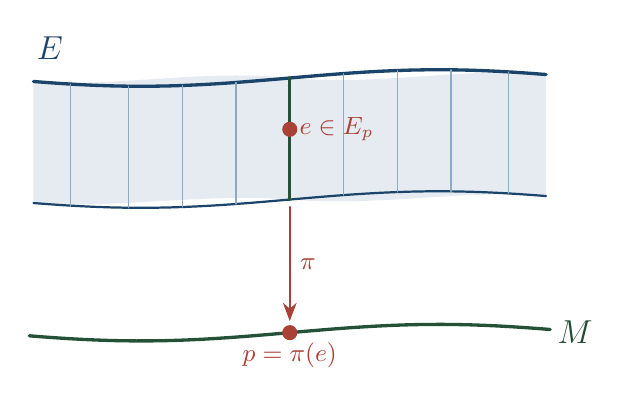
\begin{tikzpicture}[>=Stealth,scale=1.05,line cap=round]
\fill[manifoldblue!12] (-3.1,1.0)
 .. controls (-2.1,.92) and (-1.1,1.15) .. (0,1.04)
 .. controls (1.1,.94) and (2.1,1.18) .. (3.1,1.08)
 --(3.1,-.39)
 .. controls (2.1,-.30) and (1.1,-.52) .. (0,-.43)
 .. controls (-1.1,-.35) and (-2.1,-.55) .. (-3.1,-.47) --cycle;
\draw[manifoldblue!75!black,very thick]
 plot[domain=-3.1:3.1,samples=35] ({\x},{1.04+.10*sin(50*\x)});
\draw[manifoldblue!75!black,thick]
 plot[domain=-3.1:3.1,samples=35] ({\x},{-.43+.10*sin(50*\x)});
\foreach \xx in {-2.65,-1.95,-1.3,-.65,.65,1.3,1.95,2.65}
 \draw[manifoldblue!52,thin] (\xx,{-.43+.10*sin(50*\xx)})
 --(\xx,{1.04+.10*sin(50*\xx)});
\draw[manifoldgreen!65!black,very thick] (0,-.43)--(0,1.04);
\draw[manifoldgreen!65!black,very thick]
 plot[domain=-3.15:3.15,samples=40] ({\x},{-2.04+.10*sin(50*\x)});
\fill[manifoldred] (0,.42) circle (2.6pt) node[right,font=\small] {$e\in E_p$};
\fill[manifoldred] (0,-2.04) circle (2.6pt) node[below,font=\small] {$p=\pi(e)$};
\draw[->,thick,manifoldred] (0,-.52)--(0,-1.9)
 node[midway,right,font=\small] {$\pi$};
\node[manifoldblue!75!black,font=\large\bfseries] at (-2.9,1.4) {$E$};
\node[manifoldgreen!60!black,font=\large\bfseries] at (3.45,-2.03) {$M$};
\end{tikzpicture}
\caption{Lokalny obraz wiązki $\pi\colon E\to M$. Wyróżniono wektor $e$ i jego rzut $\pi(e)=p$. Włókna narysowano jako fragmenty prostych; ogólnie mają wymiar $k$.}
\label{fig:diagram-wiazki}
\end{figure}







\begin{definicja}[Trywializacja wiązki]
\index{trywializacja wiazki@Trywializacja wiązki}
Niech $\pi\colon E\to M$ będzie wiązką wektorową rzędu $k$. \emph{Trywializacją}
nad otwartym zbiorem $U\subseteq M$ nazywamy dyfeomorfizm
\[
\Phi\colon\pi^{-1}(U)\longrightarrow U\times\mathbb R^k
\]
spełniający $\operatorname{pr}_1\circ\Phi=\pi$, taki że dla każdego $p\in U$
obcięcie $\Phi|_{E_p}$ jest izomorfizmem liniowym włókna $E_p$ na
$\{p\}\times\mathbb R^k\cong\mathbb R^k$.
\end{definicja}

\begin{figure}[ht]
\centering
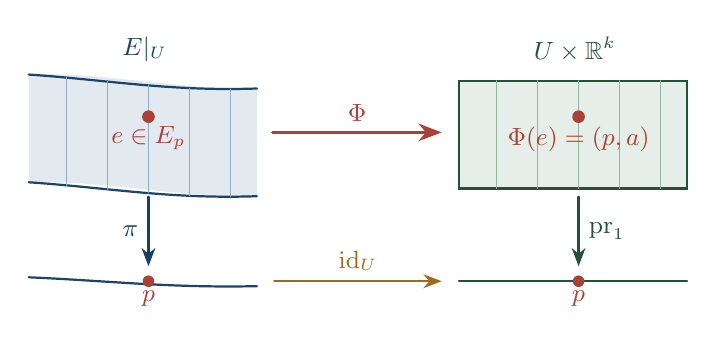
\begin{tikzpicture}[>=Stealth,scale=.95,line cap=round]
\fill[manifoldblue!13] (-4.4,1.16)
 .. controls (-3.55,1.22) and (-2.2,.93) .. (-1.35,.98)
 --(-1.35,-.46)
 .. controls (-2.2,-.51) and (-3.55,-.23) .. (-4.4,-.28) --cycle;
\draw[manifoldblue!75!black,thick]
 plot[domain=-4.4:-1.35,samples=25] ({\x},{1.08+.11*sin(52*\x)});
\draw[manifoldblue!75!black,thick]
 plot[domain=-4.4:-1.35,samples=25] ({\x},{-.36+.11*sin(52*\x)});
\foreach \xx in {-3.9,-3.35,-2.8,-2.25,-1.7}
 \draw[manifoldblue!50,thin] (\xx,{-.36+.11*sin(52*\xx)})
 --(\xx,{1.08+.11*sin(52*\xx)});
\fill[manifoldgreen!13] (1.35,-.36) rectangle (4.4,1.08);
\draw[manifoldgreen!65!black,thick] (1.35,-.36) rectangle (4.4,1.08);
\foreach \xx in {1.85,2.4,2.95,3.5,4.05}
 \draw[manifoldgreen!55,thin] (\xx,-.36)--(\xx,1.08);
\fill[manifoldred] (-2.8,.6) circle (2.4pt)
 node[below,font=\small] {$e\in E_p$};
\fill[manifoldred] (2.95,.6) circle (2.4pt)
 node[below,font=\small] {$\Phi(e)=(p,a)$};
\draw[->,very thick,manifoldred] (-1.14,.39)--(1.12,.39)
 node[midway,above,font=\small] {$\Phi$};
\draw[manifoldblue!75!black,thick]
 plot[domain=-4.4:-1.35,samples=25] ({\x},{-1.6+.07*sin(52*\x)});
\draw[manifoldgreen!65!black,thick] (1.35,-1.6)--(4.4,-1.6);
\fill[manifoldred] (-2.8,-1.6) circle (2.2pt) node[below,font=\small] {$p$};
\fill[manifoldred] (2.95,-1.6) circle (2.2pt) node[below,font=\small] {$p$};
\draw[->,manifoldblue!70!black,thick] (-2.8,-.47)--(-2.8,-1.4)
 node[midway,left,font=\small] {$\pi$};
\draw[->,manifoldgreen!65!black,thick] (2.95,-.47)--(2.95,-1.4)
 node[midway,right,font=\small] {$\operatorname{pr}_1$};
\draw[->,manifoldgold!75!black,thick] (-1.12,-1.6)--(1.12,-1.6)
 node[midway,above,font=\small] {$\mathrm{id}_U$};
\node[manifoldblue!75!black,font=\small\bfseries] at (-2.85,1.5) {$E|_U$};
\node[manifoldgreen!65!black,font=\small\bfseries] at (2.9,1.5) {$U\times\R^k$};
\end{tikzpicture}
\caption{Trywializacja $\Phi\colon E|_U\to U\times\R^k$ jest liniowa na włóknach i zachowuje punkt bazy: $\operatorname{pr}_1\circ\Phi=\pi$. Linie przedstawiają włókna schematycznie.}
\label{fig:trywializacja}
\end{figure}

\begin{definicja}[Sekcja wiązki wektorowej]
\index{sekcja wiazki wektorowej@Sekcja wiązki wektorowej}
Niech $\pi\colon E\to M$ będzie wiązką wektorową. \emph{Sekcją}
(inaczej: \emph{przekrojem}) wiązki $E$ nazywamy
gładkie odwzorowanie $s\colon M\to E$ spełniające
\[
\pi\circ s=\id_M.
\]
Zatem dla każdego $p\in M$ mamy $s(p)\in E_p$. Sekcja wybiera dokładnie jeden wektor
z każdego włókna i robi to w sposób gładki.
\end{definicja}

\begin{figure}[ht]
\centering
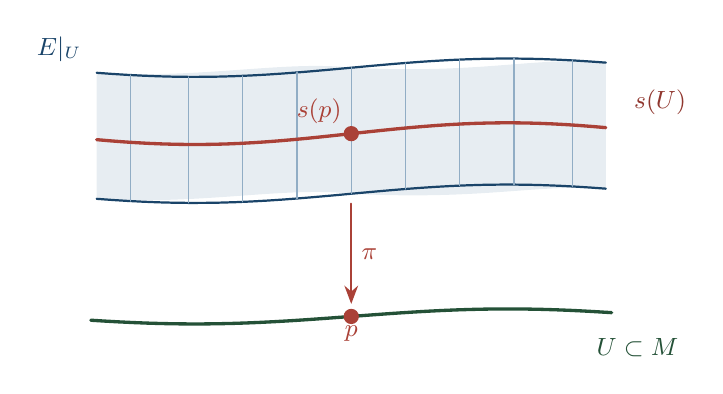
\begin{tikzpicture}[>=Stealth,scale=1.06,line cap=round]
\fill[manifoldblue!11] (-3.05,1.07)
 .. controls (-1.8,.99) and (-.8,1.22) .. (0,1.13)
 .. controls (1.6,1.05) and (2.2,1.27) .. (3.05,1.19)
 --(3.05,-.32)
 .. controls (2.2,-.26) and (1.6,-.46) .. (0,-.38)
 .. controls (-.8,-.29) and (-1.8,-.52) .. (-3.05,-.44) --cycle;
\draw[manifoldblue!75!black,thick]
 plot[domain=-3.05:3.05,samples=34] ({\x},{1.13+.11*sin(48*\x)});
\draw[manifoldblue!75!black,thick]
 plot[domain=-3.05:3.05,samples=34] ({\x},{-.38+.11*sin(48*\x)});
\foreach \xx in {-2.65,-1.95,-1.3,-.65,0,.65,1.3,1.95,2.65}
 \draw[manifoldblue!50,thin] (\xx,{-.38+.11*sin(48*\xx)})
 --(\xx,{1.13+.11*sin(48*\xx)});
\draw[manifoldgreen!65!black,very thick]
 plot[domain=-3.12:3.12,samples=38] ({\x},{-1.85+.09*sin(48*\x)});
\draw[manifoldred,very thick]
 plot[domain=-3.05:3.05,samples=40] ({\x},{.34+.13*sin(48*\x)});
\fill[manifoldred] (0,.34) circle (2.6pt) node[above left,font=\small] {$s(p)$};
\fill[manifoldred] (0,-1.85) circle (2.6pt) node[below,font=\small] {$p$};
\draw[->,manifoldred,thick] (0,-.5)--(0,-1.7)
 node[midway,right,font=\small] {$\pi$};
\node[font=\small\bfseries,manifoldred!85!black] at (3.7,.72) {$s(U)$};
\node[font=\small\bfseries,manifoldgreen!65!black] at (3.43,-2.22) {$U\subset M$};
\node[font=\small,manifoldblue!75!black] at (-3.5,1.35) {$E|_U$};
\end{tikzpicture}
\caption{Sekcja $s$ wybiera dokładnie jeden wektor $s(p)$ w każdym włóknie nad $p$. Czerwona krzywa przedstawia jej obraz nad pokazanym fragmentem $U$.}
\label{fig:sekcja}
\end{figure}

\begin{przyklad}[Sekcja zerowa]
Każda wiązka wektorowa posiada naturalną \emph{sekcję zerową}
\[
s_0\colon M\to E,\qquad s_0(p)=0_p,
\]
gdzie $0_p$ jest wektorem zerowym we włóknie $E_p$.
Gładkość wynika z lokalnego zapisu $p\mapsto(p,0)$.
\end{przyklad}


\begin{przyklad}[Wiązka trywialna]
Najprostszym przykładem jest $E=M\times\R^k$ z $\pi=\mathrm{pr}_1$ i $\Psi=\id$ — wiązka ta
nosi nazwę \emph{trywialnej}.
\end{przyklad}

Izomorfizmem wiązek nad $M$ nazywamy dyfeomorfizm przestrzeni
całkowitych zachowujący punkt bazy i liniowy na każdym włóknie.
Nie każda wiązka wektorowa jest (globalnie) izomorficzna z wiązką trywialną — mimo że
lokalnie, z definicji, każda wiązka ,,wygląda jak'' trywialna. Poniższy klasyczny przykład
ilustruje to zjawisko w najprostszym możliwym przypadku.

\begin{przyklad}[Wstęga Möbiusa jako nietrywialna wiązka rzędu 1]\label{prz:mobius}
Niech $M=S^1=\R/2\pi\Z$. Wstęgę Möbiusa można zdefiniować jako przestrzeń
ilorazową
\[
E:=\big([0,2\pi]\times\R\big)\big/\!\sim,
\qquad
(0,t)\sim(2\pi,-t),
\]
z rzutowaniem
\[
\pi\colon E\longrightarrow S^1,\qquad
\pi([\theta,t])=[\theta].
\]
Włókno nad punktem $[\theta]\in S^1$ jest kopią $\R$:
\[
E_{[\theta]}=\pi^{-1}([\theta])\cong\R.
\]
W szczególności $E$ ma wymiar $2$, natomiast baza $S^1$ ma wymiar $1$.

\medskip
\emph{Dlaczego jest to wiązka wektorowa?}
Jeżeli $I\subset S^1$ jest otwartym łukiem, który nie zawiera punktu
odpowiadającego jednocześnie $\theta=0$ i $\theta=2\pi$, można wybrać jednoznacznego
reprezentanta kąta $\theta$ w przedziale odpowiadającym $I$. Wtedy
\[
\Psi_I\colon \pi^{-1}(I)\longrightarrow I\times\R,
\qquad
[\theta,t]\longmapsto([\theta],t)
\]
jest lokalną trywializacją i na każdym włóknie jest izomorfizmem liniowym.
Także punkt sklejenia ma trywializację. Na łuku
$I_0=\{[a]:-\varepsilon<a<\varepsilon\}$, gdzie $0<\varepsilon<\pi$,
jej odwrotność jest dana przez
\[
 ([a],v)\longmapsto
 \begin{cases}
 [a,v],&a\geq0,\\
 [a+2\pi,-v],&a<0.
 \end{cases}
\]
W punkcie $a=0$ zgodność zapewnia identyfikacja końców.
Jest to homeomorfizm z $I_0\times\R$ na $\pi^{-1}(I_0)$:
w topologii ilorazowej otoczenie sklejonego punktu obejmuje
oba przyległe półpasy. Przejścia z poprzednią trywializacją
są $(p,v)\mapsto(p,v)$ po jednej stronie łuku i
$(p,v)\mapsto(p,-v)$ po drugiej, więc są gładkie.
Te mapy określają strukturę gładką na $E$. Punkty o różnych
podstawach rozdzielamy otoczeniami w $S^1$, a punkty tego samego
włókna w jednej trywializacji; zatem $E$ jest Hausdorffa.
Dwie trywializacje nad łukami dają przeliczalną bazę $E$.
Po obejściu całej bazy współrzędna włókna zmienia znak:
\[
t\longmapsto -t.
\]
Jest to istotna informacja globalna: lokalnie wiązka jest nierozróżnialna od
$S^1\times\R$, ale globalnie nie można wybrać w niej spójnie jednego kierunku
w każdym włóknie.

W języku funkcji przejścia można to zapisać jeszcze prościej. Dla wiązki rzędu $1$
funkcje przejścia przyjmują wartości w
$\mathrm{GL}(1,\R)=\R_*$. W przypadku wstęgi Möbiusa pojawia się
przejście
\[
g=-1,
\]
podczas gdy dla wiązki trywialnej można wybrać $g=+1$. Znak $-1$ jest właśnie
algebraicznym zapisem ``odwrócenia'' włókna przy jednym pełnym okrążeniu bazy.
\end{przyklad}

\begin{figure}[h]
\centering
\begin{minipage}{0.43\textwidth}
\centering
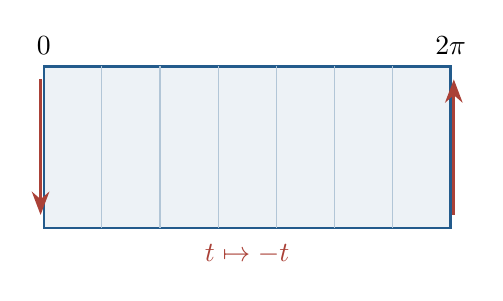
\begin{tikzpicture}[>=Stealth,scale=0.82]
  \fill[manifoldblue!8] (0,-1.25) rectangle (6.3,1.25);
  \draw[thick,manifoldblue] (0,-1.25) rectangle (6.3,1.25);
  \foreach \x in {0.9,1.8,2.7,3.6,4.5,5.4}
    \draw[manifoldblue!35] (\x,-1.25)--(\x,1.25);
  \draw[very thick,->,manifoldred] (-0.05,1.05) -- (-0.05,-1.05);
  \draw[very thick,->,manifoldred] (6.35,-1.05) -- (6.35,1.05);
  \node[above] at (0,1.28) {$0$};
  \node[above] at (6.3,1.28) {$2\pi$};
  \node[manifoldred] at (3.15,-1.65) {$t\mapsto-t$};
\end{tikzpicture}

\smallskip
\small (a) Prostokąt przed sklejeniem
\end{minipage}
\hfill
\begin{minipage}{0.53\textwidth}
\centering
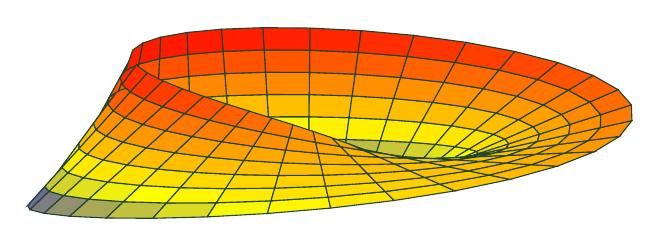
\begin{tikzpicture}
\begin{axis}[
  width=\linewidth,
  height=5.4cm,
  view={55}{25},
  axis lines=none,
  ticks=none,
  z buffer=sort,
  clip=false
]
\addplot3[
  surf,
  shader=faceted,
  faceted color=manifoldgreen!55!black,
  draw=manifoldgreen!70!black,
  domain=0:360,
  y domain=-0.55:0.55,
  samples=34,
  samples y=8
]
({(1+y*cos(x/2))*cos(x)},
 {(1+y*cos(x/2))*sin(x)},
 {y*sin(x/2)});
\end{axis}
\end{tikzpicture}

\smallskip
\small (b) Model geometryczny w $\R^3$
\end{minipage}
\caption{Wstęga Möbiusa: (a) konstrukcja przez sklejenie boków prostokąta z
odwróceniem współrzędnej włókna, (b) odpowiadająca jej klasyczna powierzchnia
zanurzona w $\R^3$. Parametryzacja w części (b) ma postać
$x=(1+t\cos(\theta/2))\cos\theta$,
$y=(1+t\cos(\theta/2))\sin\theta$,
$z=t\sin(\theta/2)$. Rysunek pokazuje tylko pas $|t|\leq0.55$;
w całej wiązce wektorowej $t$ przebiega $\R$.}
\label{fig:mobius}
\end{figure}

\begin{stwierdzenie}[Nietrywialność wstęgi Möbiusa]
Wiązka $E$ z Przykładu~\ref{prz:mobius} nie jest izomorficzna jako wiązka wektorowa
z wiązką trywialną $S^1\times\R$.
\end{stwierdzenie}

\begin{proof}
Niech $q\colon[0,2\pi]\times\R\to E$ oznacza rzutowanie ilorazowe. Każdej ciągłej
funkcji $f\colon[0,2\pi]\to\R$ spełniającej
\[
f(2\pi)=-f(0)
\]
odpowiada ciągły przekrój
\[
s_f\colon S^1\to E,\qquad s_f([\theta])=q(\theta,f(\theta)).
\]
Warunek brzegowy jest dokładnie warunkiem dobrze określoności w punkcie sklejenia.
Odwrotnie, każdy ciągły przekrój ma tę postać: nad przedziałem
$[0,2\pi]$ wybieramy współrzędną włóknową $t$, a ciągłość w
trywializacji przy sklejeniu daje ciągłość $f$ i podany warunek końcowy.
Przekrój jest gładki dokładnie wtedy, gdy $f$ jest gładka na
przedziale (z jednostronnymi pochodnymi na końcach) i
$f^{(j)}(2\pi)=-f^{(j)}(0)$ dla każdego $j\geq0$.
Sam warunek na wartości zapewnia ciągłość, lecz nie gładkość.

Załóżmy, że $s_f$ jest nigdzie zerowa. Wtedy $f$ nie przyjmuje wartości $0$.
Ponieważ $[0,2\pi]$ jest spójny, a $f$ jest ciągła, z twierdzenia o wartości
pośredniej wynika, że $f$ ma stały znak. W szczególności $f(0)$ i $f(2\pi)$
mają ten sam znak. Jest to niemożliwe, gdyż
$f(2\pi)=-f(0)$ i $f(0)\neq0$.

Zatem $E$ nie posiada nigdzie niezerowej sekcji. Natomiast wiązka trywialna
$S^1\times\R$ posiada taką sekcję, mianowicie
\[
s(\theta)=(\theta,1).
\]
Gdyby istniał izomorfizm wiązek
$\Psi\colon S^1\times\R\to E$, sekcja $\Psi\circ s$ byłaby nigdzie niezerową
sekcją $E$, co daje sprzeczność. Zatem
\[
E\not\cong S^1\times\R.
\]
\end{proof}

\begin{uwaga}[Interpretacja topologiczna]
Wstęga Möbiusa jest przykładem wiązki wektorowej, która jest lokalnie trywialna,
ale nie jest globalnie trywialna. To rozróżnienie jest fundamentalne:
\[
\boxed{\text{lokalnie trywialna}\ \not\Rightarrow\ \text{globalnie trywialna}.}
\]
Przestrzeń całkowita $E$, z włóknem $\R$, jest dwuwymiarową
rozmaitością \emph{bez brzegu}; bywa nazywana otwartą wstęgą Möbiusa.
Jej środkowy przekrój $\theta\mapsto[\theta,0]$ jest przekrojem zerowym.
Dopiero ograniczenie $|t|\leq c$ dla $c>0$ daje zwartą wstęgę
Möbiusa z brzegiem, widoczną na rysunku. Jej włókna są odcinkami,
więc ten ograniczony pas nie jest wiązką wektorową.
Odcinki $t=c$ i $t=-c$ sklejają się w jedną składową brzegu.
\end{uwaga}

\begin{przyklad}[Wiązka tautologiczna nad $\mathbb{RP}^1$]
Przykład wstęgi Möbiusa ma bardzo naturalny związek z przestrzenią rzutową.
Niech
\[
\gamma^1:=\{([x],v)\in\mathbb{RP}^1\times\R^2:\ v\in\operatorname{span}(x)\},
\]
gdzie $x\in\R^2\setminus\{0\}$ jest dowolnym reprezentantem klasy $[x]$.
Włókno nad $[x]$ jest zatem prostą
\[
\gamma^1_{[x]}=\operatorname{span}(x)\subset\R^2.
\]
Jest to \emph{wiązka tautologiczna} (kanoniczna wiązka liniowa) nad $\mathbb{RP}^1$.

Ponieważ $\mathbb{RP}^1$ jest dyfeomorficzna z okręgiem $S^1$, a przejście
z kierunku $x$ do tego samego kierunku po jednym pełnym okrążeniu wymusza zmianę
reprezentanta z $x$ na $-x$, wiązka $\gamma^1$ jest izomorficzna z wstęgą Möbiusa.
Jest to więc drugi, geometryczny sposób zobaczenia tej samej nietrywialnej wiązki:
w każdym punkcie przestrzeni rzutowej wybieramy \emph{linię} w $\R^2$, a nie
wyróżniony wektor tej linii.
Jawny izomorfizm nad dyfeomorfizmem baz
$[\theta]\mapsto[\cos(\theta/2):\sin(\theta/2)]$ ma postać
\[
 [\theta,t]\longmapsto
 \bigl([\cos(\theta/2):\sin(\theta/2)],
       t(\cos(\theta/2),\sin(\theta/2))\bigr).
\]
Przy zwiększeniu $\theta$ o $2\pi$ wektor jednostkowy zmienia znak,
który kompensuje identyfikacja $t\mapsto-t$. Wzór jest więc dobrze
określony. W każdym łuku wybieramy gładko ten wektor jednostkowy;
wtedy odwrotność odczytuje współczynnik $t$, co dowodzi gładkości
obu kierunków i liniowości na włóknach.
\end{przyklad}

\subsection*{Wiązka styczna}

Pokażemy, że zbiór $TM:=\bigsqcup_{p\in M}T_pM$ można w naturalny sposób wyposażyć w
strukturę rozmaitości gładkiej wymiaru $2n$, tak by rzutowanie $\pi\colon TM\to M$,
$\pi(v)=p$ dla $v\in T_pM$, było wiązką wektorową rzędu $n$.

Niech $\{(U_\alpha,\varphi_\alpha)\}$ będzie atlasem na $M$, $\varphi_\alpha=(x^1_\alpha,
\dots,x^n_\alpha)$. Definiujemy $\tilde U_\alpha:=\pi^{-1}(U_\alpha)\subseteq TM$ oraz
\[
\tilde\varphi_\alpha\colon\tilde U_\alpha\to\varphi_\alpha(U_\alpha)\times\R^n\subseteq
\R^{2n}, \qquad \tilde\varphi_\alpha\Big(\sum_{i=1}^nv^i\,\frac{\partial}{\partial
x^i_\alpha}\Big|_p\Big):=(\varphi_\alpha(p),\,v^1,\dots,v^n).
\]
Każde $\tilde\varphi_\alpha$ jest bijekcją na $\varphi_\alpha(U_\alpha)\times\R^n$ (dla
ustalonego $p$, współrzędne $v^i$ względem bazy $\{\partial/\partial x^i_\alpha|_p\}$
wyznaczają bijekcję liniową $T_pM\to\R^n$).

Obliczmy odwzorowanie przejścia $\tilde\varphi_\beta\circ\tilde\varphi_\alpha^{-1}$. Ze
wzoru na zmianę bazy pochodnych cząstkowych (reguła łańcucha zastosowana do funkcji
przejścia $\varphi_\beta\circ\varphi_\alpha^{-1}$):
\[
\frac{\partial}{\partial x^i_\alpha}\bigg|_p=\sum_{j=1}^n\frac{\partial x^j_\beta}
{\partial x^i_\alpha}(\varphi_\alpha(p))\;\frac{\partial}{\partial x^j_\beta}\bigg|_p
\]
(równość ta jest bezpośrednią konsekwencją definicji $\partial/\partial x^i_\alpha|_p$ jako
funkcjonału $f\mapsto\partial(f\circ\varphi_\alpha^{-1})/\partial x^i(\varphi_\alpha(p))$
oraz reguły łańcucha dla $f\circ\varphi_\alpha^{-1}=(f\circ\varphi_\beta^{-1})\circ
(\varphi_\beta\circ\varphi_\alpha^{-1})$). Zatem wektor $v=\sum_iv^i\,\partial/\partial
x^i_\alpha|_p$ ma we współrzędnych $\beta$ postać $w^j=\sum_i\frac{\partial x^j_\beta}
{\partial x^i_\alpha}(\varphi_\alpha(p))\,v^i$, czyli $w=D(\varphi_\beta\circ
\varphi_\alpha^{-1})(\varphi_\alpha(p))\cdot v$. Stąd
\[
\big(\tilde\varphi_\beta\circ\tilde\varphi_\alpha^{-1}\big)(x,v)=\Big(
(\varphi_\beta\circ\varphi_\alpha^{-1})(x),\ D(\varphi_\beta\circ\varphi_\alpha^{-1})(x)
\cdot v\Big).
\]
Najpierw określamy topologię na $TM$: zbiór $A\subset TM$
jest otwarty wtedy i tylko wtedy, gdy każdy
$\tilde\varphi_\alpha(A\cap\tilde U_\alpha)$ jest otwarty.
Zmiany współrzędnych powyżej są homeomorfizmami, a ich dziedziny
$\varphi_\alpha(U_\alpha\cap U_\beta)\times\R^n$ są otwarte.
Wynika stąd, że $\tilde U_\alpha$ są otwarte, a
$\tilde\varphi_\alpha$ są homeomorfizmami: obraz dowolnego otwartego
zbioru z jednej mapy jest otwarty także w każdej nakładającej się mapie.
Rzutowanie $\pi$ jest ciągłe, bo lokalnie ma postać $(x,v)\mapsto x$.
Powyższa zmiana współrzędnych jest gładka: pierwsza składowa jest gładka jako odwzorowanie przejścia
atlasu na $M$; druga jest liniowa w $v$ ze współczynnikami będącymi pochodnymi cząstkowymi
$\varphi_\beta\circ\varphi_\alpha^{-1}$, a więc gładkimi funkcjami $x$. Zatem $\{(\tilde
U_\alpha,\tilde\varphi_\alpha)\}$ jest atlasem na $TM$. Punkty o różnych
podstawach rozdzielają przeciwobrazy rozłącznych otoczeń w $M$;
dwa różne wektory w jednym włóknie rozdzielają kule w jednej mapie
$\tilde\varphi_\alpha$. Stąd $TM$ jest Hausdorffa. Z przeliczalności
bazy $M$ wybieramy przeliczalną rodzinę dziedzin map pokrywającą $M$.
Obrazy tych map w $TM$ mają przeliczalne bazy euklidesowe, których
przeciwobrazy tworzą przeliczalną bazę $TM$.

Tak skonstruowana rozmaitość $TM$, wraz z rzutowaniem $\pi$ i lokalnymi trywializacjami
$\Psi_\alpha=(\varphi_\alpha^{-1}\times\id)\circ\tilde\varphi_\alpha$, jest wiązką
wektorową rzędu $n$ nad $M$ — \emph{wiązką styczną}.

Analogicznie definiuje się \emph{wiązkę kostyczną} $T^*M:=\bigsqcup_{p\in M}T_p^*M$, z
mapami $\tilde\varphi_\alpha^*\big(\sum_i\xi_i\,dx^i_\alpha|_p\big):=(\varphi_\alpha(p),
\xi_1,\dots,\xi_n)$. Odwzorowanie przejścia oblicza się analogicznie — współczynniki
$\xi_i$ transformują się \emph{kowariantnie}: jeśli $\omega=\sum_i\xi_i^\alpha
dx^i_\alpha|_p=\sum_j\xi_j^\beta dx^j_\beta|_p$, to z reguły łańcucha $dx^i_\alpha|_p=
\sum_j\frac{\partial x^i_\alpha}{\partial x^j_\beta}(\varphi_\beta(p))\,dx^j_\beta|_p$,
skąd $\xi_j^\beta=\sum_i\xi_i^\alpha\frac{\partial x^i_\alpha}{\partial x^j_\beta}
(\varphi_\beta(p))$ — co ponownie daje gładkie odwzorowania przejścia. Dowód, że $T^*M$
jest wiązką wektorową rzędu $n$ nad $M$, dopełnia to samo sprawdzenie:
punkty o różnych podstawach rozdzielają przeciwobrazy otoczeń bazy,
punkty jednego włókna rozdzielają kule współrzędnych dualnych; bazy
euklidesowe w przeliczalnym pokryciu map dają drugi aksjomat przeliczalności.

\begin{definicja}
\emph{Polem wektorowym} na $M$ nazywamy gładką sekcję wiązki stycznej, tzn.\ gładkie
odwzorowanie $X\colon M\to TM$ z $\pi\circ X=\id_M$ (a więc $X(p)\in T_pM$ dla każdego
$p$). \emph{Polem kowektorowym} na $M$ nazywamy gładką sekcję wiązki kostycznej $T^*M$.
\end{definicja}
\section{Funkcje przejścia i operacje na wiązkach}

Lokalna trywialność pozwala opisywać wiązkę macierzami. Ta postać jest
szczególnie użyteczna przy konstruowaniu wiązek normalnych podrozmaitości.
Niech $\Psi_i:E|_{U_i}\to U_i\times\R^r$ będą trywializacjami i zapiszmy
\[
\Psi_j\Psi_i^{-1}(p,v)=(p,g_{ji}(p)v),\qquad
g_{ji}:U_i\cap U_j\longrightarrow\mathrm{GL}(r,\R).
\]
Macierze $g_{ji}$ są gładkie; na przecięciach spełniają
\[
g_{ii}=I,\qquad g_{ij}=g_{ji}^{-1},\qquad
g_{ki}=g_{kj}g_{ji}\quad\text{na }U_i\cap U_j\cap U_k.
\tag{1.1}
\]
Ostatnia równość porównuje bezpośrednie przejście z $i$ do $k$
z przejściem przez $j$; nazywamy ją warunkiem kocyklu.

\begin{twierdzenie}[Sklejanie wiązki z funkcji przejścia]
Niech $\{U_i\}$ będzie otwartym pokryciem rozmaitości $M$, a gładkie funkcje
$g_{ji}:U_i\cap U_j\to\mathrm{GL}(r,\R)$ spełniają (1.1). Wtedy istnieje
wiązka wektorowa rzędu $r$ o tych funkcjach przejścia.
\end{twierdzenie}
\begin{proof}
W sumie rozłącznej $\bigsqcup_i(U_i\times\R^r)$ utożsamiamy
$(p,v)_i$ z $(p,g_{ji}(p)v)_j$ dla $p\in U_i\cap U_j$. To rzeczywiście
relacja równoważności: pierwsza i druga tożsamość w (1.1) dają zwrotność
i symetrię, trzecia daje przechodniość. Niech $E$ będzie zbiorem klas i
$\pi([p,v]_i)=p$. Dla każdego $i$ odwzorowanie
\[
\Psi_i:\pi^{-1}(U_i)\longrightarrow U_i\times\R^r,\qquad
\Psi_i([p,v]_j)=(p,g_{ij}(p)v)
\]
jest dobrze określone: jeżeli $(p,v)_j\sim(p,w)_k$, to $w=g_{kj}v$,
a $g_{ik}w=g_{ik}g_{kj}v=g_{ij}v$. Odwrotność wysyła $(p,v)$ na
$[p,v]_i$. Nadajemy $E$ topologię, deklarując $A\subset E$ otwartym,
gdy każde $\Psi_i(A\cap\pi^{-1}(U_i))$ jest otwarte w $U_i\times\R^r$.
Zmiany trywializacji są homeomorfizmami między otwartymi podzbiorami,
więc każda $\pi^{-1}(U_i)$ jest otwarta, a $\Psi_i$ jest homeomorfizmem.
Łącząc $\Psi_i$ z mapami bazy $U_i$, otrzymujemy mapy do $\R^{\dim M+r}$.
Na przecięciach zmiana współrzędnych to dokładnie
$(p,v)\mapsto(p,g_{ji}(p)v)$, więc jest gładka i ma gładką odwrotność.
Włókna dostają działania liniowe przeniesione z $\R^r$; są niezależne
od wyboru trywializacji, bo $g_{ji}(p)$ jest liniowa. Otrzymujemy żądaną wiązkę.
Uzasadnijmy jeszcze dwie własności topologiczne. Punkty o różnych obrazach
w $M$ rozdzielamy przeciwobrazami rozłącznych otwartych otoczeń bazy;
punkty jednego włókna rozdzielamy we wspólnej trywializacji, wybierając
rozłączne otwarte kule wokół ich współrzędnych włóknowych. Stąd $E$ jest
Hausdorffa. Z drugiej przeliczalności $M$ wynika istnienie przeliczalnego
podpokrycia spośród $U_i$: dla każdego elementu przeliczalnej bazy,
który mieści się w jakimś $U_i$, wybieramy jeden taki $U_i$.
Te wybrane zbiory pokrywają $M$. Każde $U_i\times\R^r$
z podpokrycia ma
przeliczalną bazę, której obrazy przez $\Psi_i^{-1}$ razem dają
przeliczalną bazę $E$.
\end{proof}

\begin{figure}[ht]
\centering
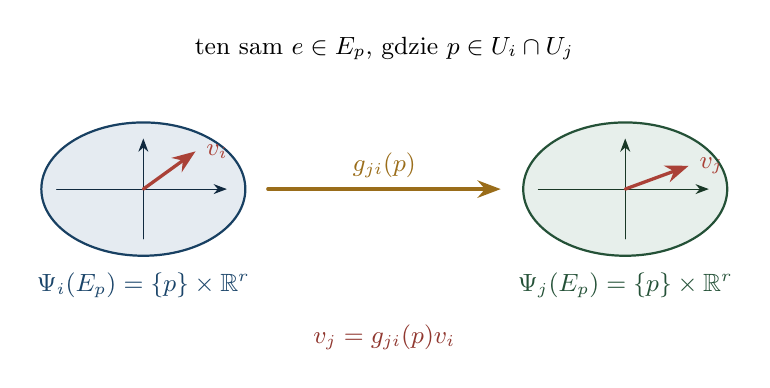
\begin{tikzpicture}[>=Stealth,scale=1.02,line cap=round]
\node[font=\small] at (0,1.75) {ten sam $e\in E_p$, gdzie $p\in U_i\cap U_j$};
\fill[manifoldblue!12] (-3,0) ellipse (1.27 and .83);
\draw[manifoldblue!70!black,thick] (-3,0) ellipse (1.27 and .83);
\draw[->,manifoldblue!45!black,thin] (-4.08,0)--(-1.96,0);
\draw[->,manifoldblue!45!black,thin] (-3,-.62)--(-3,.63);
\draw[->,manifoldred,very thick] (-3,0)--(-2.35,.47)
 node[right,font=\small] {$v_i$};
\fill[manifoldgreen!12] (3,0) ellipse (1.27 and .83);
\draw[manifoldgreen!65!black,thick] (3,0) ellipse (1.27 and .83);
\draw[->,manifoldgreen!45!black,thin] (1.92,0)--(4.04,0);
\draw[->,manifoldgreen!45!black,thin] (3,-.62)--(3,.63);
\draw[->,manifoldred,very thick] (3,0)--(3.79,.29)
 node[right,font=\small] {$v_j$};
\draw[->,very thick,manifoldgold!75!black] (-1.45,0)--(1.45,0)
 node[midway,above,font=\small] {$g_{ji}(p)$};
\node[font=\small,manifoldblue!75!black] at (-3,-1.2)
 {$\Psi_i(E_p)=\{p\}\times\R^r$};
\node[font=\small,manifoldgreen!65!black] at (3,-1.2)
 {$\Psi_j(E_p)=\{p\}\times\R^r$};
\node[font=\small\bfseries,manifoldred!85!black] at (0,-1.85)
 {$v_j=g_{ji}(p)v_i$};
\end{tikzpicture}
\caption{Dwie trywializacje tego samego włókna $E_p$. Wektor $e$ ma współrzędne $v_i$ i $v_j$, związane macierzą przejścia $g_{ji}(p)$.}
\end{figure}

\begin{uwaga}[Grupa strukturalna]
Wybór baz włókien daje funkcje o wartościach w $\mathrm{GL}(r,\R)$; jest to
naturalna grupa strukturalna wiązki rzędu $r$. Jeżeli można dobrać
trywializacje tak, aby wszystkie macierze przejścia należały do podgrupy
$G\subseteq\mathrm{GL}(r,\R)$, mówimy o redukcji grupy strukturalnej do $G$.
Na przykład lokalne bazy ortonormalne wiązki z iloczynem skalarnym mają
macierze przejścia w $\mathrm{O}(r)$. Dla wiązki liniowej przejście $-1$
po okrążeniu okręgu wyraża skręcenie wstęgi Möbiusa.
\end{uwaga}

\begin{przyklad}[Sekcje w zapisie lokalnym]
Sekcja $s$ zapisuje się w trywializacji nad $U_i$ jako $s_i:U_i\to\R^r$. Na
przecięciu $s_j(p)=g_{ji}(p)s_i(p)$. Odwrotnie, rodzina gładkich funkcji
$s_i$ spełniająca te równości wyznacza jedną sekcję $s(p)=[p,s_i(p)]_i$;
niezależność od indeksu to dokładnie warunek zgodności. Dla wstęgi
Möbiusa można wybrać współrzędną na przedziale $[0,2\pi]$ i otrzymać
warunek $s(2\pi)=-s(0)$. Ciągła funkcja rzeczywista spełniająca ten
warunek musi mieć zero: jeśli wartość w początku jest niezerowa,
na końcu ma przeciwny znak, więc stosujemy twierdzenie o wartości
pośredniej; jeśli jest zerowa, teza jest natychmiastowa.
\end{przyklad}

\begin{definicja}[Suma i wiązka dualna]
\index{suma i wiazka dualna@Suma i wiązka dualna}
Dla wiązek $E,F$ nad tą samą bazą definiujemy włókna
$(E\oplus F)_p=E_p\oplus F_p$ oraz
$(E^*)_p=\mathrm{Hom}(E_p,\R)$. Przy macierzach przejścia $g_{ji}$
i $h_{ji}$ odpowiednie macierze to
\[
g_{ji}\oplus h_{ji},\qquad(g_{ji}^{-1})^{\mathsf T}.
\]
Ostatni wzór wymusza zachowanie wartości funkcjonału:
jeżeli $v_j=g_{ji}v_i$ oraz $\xi_i(v_i)=\xi_j(v_j)$, to
$\xi_j=(g_{ji}^{-1})^{\mathsf T}\xi_i$. Obie rodziny spełniają
warunek kocyklu, więc twierdzenie o sklejaniu tworzy z nich wiązki.
\end{definicja}



\section{Różniczka, immersje, submersje i zanurzenia}

\begin{definicja}
Niech $F\colon M\to N$ będzie odwzorowaniem gładkim, $p\in M$. \emph{Różniczką} $F$ w
punkcie $p$ nazywamy odwzorowanie liniowe $dF_p\colon T_pM\to T_{F(p)}N$ zdefiniowane (w
języku derywacji) wzorem
\[
(dF_p\,v)(g):=v(g\circ F), \qquad v\in T_pM,\ g\in C^\infty(N).
\]
\end{definicja}

\begin{fakt}
$dF_pv$ jest istotnie derywacją w $F(p)$, a $dF_p$ jest odwzorowaniem liniowym.
\end{fakt}
\begin{proof}
Liniowość względem $g$: oczywista z liniowości $v$ i liniowości $g\mapsto g\circ F$.
Reguła Leibniza: $(dF_pv)(gh)=v((gh)\circ F)=v((g\circ F)(h\circ F))=(g\circ F)(p)\,
v(h\circ F)+(h\circ F)(p)\,v(g\circ F)=g(F(p))(dF_pv)(h)+h(F(p))(dF_pv)(g)$, na mocy reguły
Leibniza dla $v$ zastosowanej do $g\circ F,h\circ F\in C^\infty(M)$. Zatem $dF_pv\in
T_{F(p)}N$. Liniowość $dF_p$ względem $v$ jest natychmiastowa z liniowości $v\mapsto
v(g\circ F)$ w $v$, dla każdego ustalonego $g$.
\end{proof}

\begin{twierdzenie}[Reguła łańcucha]
Jeśli $F\colon M\to N$ i $G\colon N\to P$ są gładkie, $p\in M$, to
\[
d(G\circ F)_p=dG_{F(p)}\circ dF_p\colon T_pM\to T_{G(F(p))}P.
\]
\end{twierdzenie}
\begin{proof}
Dla $v\in T_pM$ i $h\in C^\infty(P)$, z definicji różniczki:
\[
\big(d(G\circ F)_p\,v\big)(h)=v\big(h\circ(G\circ F)\big)=v\big((h\circ G)\circ F\big)=
(dF_pv)(h\circ G)=\big(dG_{F(p)}(dF_pv)\big)(h),
\]
gdzie w trzeciej równości zastosowaliśmy definicję $dF_p$ do $h\circ G\in C^\infty(N)$, a
w czwartej — definicję $dG_{F(p)}$ do $dF_pv\in T_{F(p)}N$. Zatem $d(G\circ F)_pv=
dG_{F(p)}(dF_pv)$ dla każdego $v$ — co dowodzi tezy.
\end{proof}

\begin{uwaga}[Skąd bierze się macierz Jacobiego?]
W mapach $(U,\varphi)$ o współrzędnych $(x^1,\ldots,x^m)$ wokół $p$ i
$(V,\psi)$ o współrzędnych $(y^1,\ldots,y^n)$ wokół $F(p)$ niech
$\widehat F=\psi\circ F\circ\varphi^{-1}$.
Aby znaleźć współczynniki $dF_p(\partial/\partial x^i|_p)$
w bazie $\partial/\partial y^a|_{F(p)}$, przykładamy ten
wektor do funkcji współrzędnej $y^a$ (lokalnie; w razie
potrzeby przedłużamy ją funkcją odcinającą). Z definicji
różniczki otrzymujemy
\[
 \bigl(dF_p(\partial/\partial x^i|_p)\bigr)(y^a)
 =\left.\frac{\partial \widehat F^{\,a}}{\partial x^i}
 \right|_{\varphi(p)}.
\]
Współczynniki te tworzą macierz Jacobiego
$D\widehat F(\varphi(p))$. \emph{Rzędem} $F$ w punkcie $p$
nazywamy rząd $dF_p$, równy rzędowi tej macierzy.
\end{uwaga}

\begin{definicja}
Niech $F\colon M\to N$ będzie gładkie, $\dim M=m$, $\dim N=n$. Mówimy, że $F$ jest w
punkcie $p$ \emph{immersją}, jeśli $dF_p$ jest injektywne, oraz \emph{submersją}, jeśli
$dF_p$ jest surjektywne. $F$ jest immersją (submersją), jeśli jest nią w każdym punkcie
$p\in M$. \emph{Zanurzeniem} (ang.\ \emph{embedding}) nazywamy immersję $F\colon M\to N$,
która dodatkowo jest homeomorfizmem na obraz $F(M)$ (z topologią podprzestrzeni $N$).
\end{definicja}

Poniższy przykład pokazuje, że sama różnowartościowa immersja nie musi być zanurzeniem —
warunek ,,homeomorfizm na obraz'' jest istotnie mocniejszy.

\begin{przyklad}[Krzywa ósemkowa]\label{prz:osemka}
Niech $\beta\colon(-\pi,\pi)\to\R^2$, $\beta(t):=(\sin2t,\ \sin t)$.

\emph{$\beta$ jest immersją.} $\beta'(t)=(2\cos2t,\cos t)$. Gdyby $\beta'(t_0)=0$, to
$\cos t_0=0$ (więc $t_0=\pm\pi/2$) oraz $\cos2t_0=0$; ale $\cos(\pm\pi)=-1\neq0$ —
sprzeczność. Zatem $\beta'(t)\neq0$ dla wszystkich $t$, czyli $d\beta_t$ jest injektywne w
każdym punkcie.

\emph{$\beta$ jest różnowartościowa.} Przypuśćmy $\beta(t_1)=\beta(t_2)$, tzn.\ $\sin t_1=
\sin t_2=:s$ oraz $\sin2t_1=\sin2t_2$. Jeśli $s=0$: na $(-\pi,\pi)$ równość $\sin t=0$
zachodzi jedynie dla $t=0$, więc $t_1=t_2=0$. Jeśli $s\neq0$: korzystając z $\sin2t_i=
2\sin t_i\cos t_i=2s\cos t_i$, równość $\sin2t_1=\sin2t_2$ daje (dzieląc przez $2s\neq0$)
$\cos t_1=\cos t_2$. Zatem $\sin t_1=\sin t_2$ i $\cos t_1=\cos t_2$ jednocześnie — co
oznacza $t_1-t_2\in2\pi\Z$; ponieważ $t_1,t_2\in(-\pi,\pi)$, jedyna możliwość to $t_1=t_2$.
W obu przypadkach $\beta$ jest różnowartościowa.

\emph{$\beta$ nie jest zanurzeniem.} $\lim_{t\to\pi^-}\beta(t)=(\sin2\pi,\sin\pi)=(0,0)$
oraz $\lim_{t\to-\pi^+}\beta(t)=(0,0)$ — oba końce krzywej zbiegają do tego samego punktu
$(0,0)=\beta(0)$. Odwzorowanie odwrotne $\beta^{-1}$ nie jest więc ciągłe w $(0,0)$: dla
ciągu $t_k\to\pi^-$, $\beta(t_k)\to(0,0)=\beta(0)$, ale $\beta^{-1}(\beta(t_k))=t_k\to\pi
\neq0=\beta^{-1}(0,0)$. Zatem $\beta$ jest różnowartościową immersją, która nie jest
homeomorfizmem na obraz — nie jest zanurzeniem.
\end{przyklad}

\begin{figure}[h]
\centering
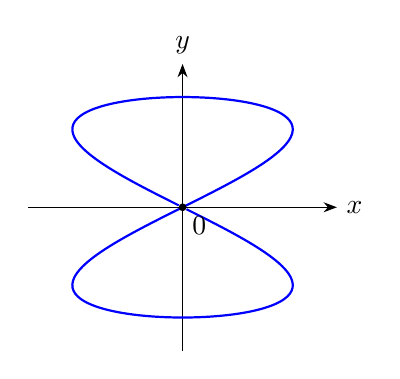
\begin{tikzpicture}[>=Stealth,scale=1.4]
\draw[->] (-1.4,0) -- (1.4,0) node[right]{$x$};
\draw[->] (0,-1.3) -- (0,1.3) node[above]{$y$};
\draw[thick,blue,domain=-179:179,samples=150,smooth]
plot ({sin(2*\x)},{sin(\x)});
\fill (0,0) circle (1pt) node[below right]{$0$};
\end{tikzpicture}
\caption{Krzywa ósemkowa $\beta(t)=(\sin2t,\sin t)$: różnowartościowa immersja, która nie
jest zanurzeniem — oba końce ($t\to\pm\pi$) zbiegają do początku układu współrzędnych.}
\label{fig:osemka}
\end{figure}

\begin{uwaga}
Podobny, choć bardziej subtelny, przykład daje \emph{nawinięcie niewymierne} torusa
$T^2=\R^2/\Z^2$: krzywa $\gamma(t)=(t,\alpha t)+\Z^2$
dla $\alpha\in\R\setminus\Q$ jest injektywną immersją.
Rzeczywiście $\gamma(t)=\gamma(s)$ wymaga $t-s\in\Z$ i
$\alpha(t-s)\in\Z$, więc $t=s$; lokalna pochodna to $(1,\alpha)\ne0$.
Pokażmy wprost brak ciągłości odwrotności. Dzieląc $[0,1)$ na
$N$ równych przedziałów i rozpatrując części ułamkowe
$0,\alpha,\ldots,N\alpha$, z zasady szufladkowej otrzymujemy
$1\leq q_N\leq N$ oraz $p_N\in\Z$ takie, że
$|q_N\alpha-p_N|<1/N$. Możemy wybrać podciąg z $q_N\to\infty$:
dla skończenie wielu dodatnich $q$ odległości $q\alpha$ od $\Z$
mają dodatnie minimum. Wtedy $\gamma(q_N)\to\gamma(0)$,
ale $q_N$ nie dąży do zera, więc odwrotność nie jest ciągła.
Obraz jest również gęsty. Istotnie, dla dowolnie małego $\varepsilon>0$
istnieje niezerowe $\delta=q\alpha-p$ z $|\delta|<\varepsilon$.
Wielokrotności $\delta$ modulo $1$ tworzą zbiór
$\varepsilon$-gęsty w okręgu (kolejne punkty są oddalone o
$|\delta|$, a ostatnia luka jest nie większa).
Są to części ułamkowe całkowitych wielokrotności $\alpha$.
Zatem dla dowolnego $(a,b)+\Z^2$ można dobrać $k\in\Z$,
aby $\gamma(a+k)=(a,\alpha a+\alpha k)+\Z^2$ było dowolnie
blisko tego punktu.
\end{uwaga}

\subsection*{Twierdzenie o rzędzie stałym}

\begin{lemat}[Półciągłość rzędu z dołu]\label{lem:polciaglosc}
Niech $F\colon M\to N$ będzie gładkie. Zbiór $\{p\in M:\mathrm{rz}(dF_p)\geq r\}$ jest
otwarty w $M$, dla każdego $r$.
\end{lemat}
\begin{proof}
Warunek $\mathrm{rz}(dF_p)\geq r$ oznacza, w mapach lokalnych, że macierz Jacobiego $DF$ w
$\varphi(p)$ ma pewien minor stopnia $r$ różny od zera. Wyznacznik danego minora jest
funkcją ciągłą (wielomianem od wyrazów macierzy Jacobiego, gładkich funkcji punktu), więc
zbiór punktów, w których ten minor jest niezerowy, jest otwarty. Zbiór $\{\mathrm{rz}
(dF_p)\geq r\}$ jest sumą (po wszystkich wyborach minora stopnia $r$) takich zbiorów
otwartych, a więc otwarty.
\end{proof}

\begin{wniosek}\label{wn:stalyrzad}
Jeśli $F\colon M\to N$ jest immersją (submersją) w punkcie $p$, to $F$ jest immersją
(submersją) na pewnym otoczeniu $p$, o \emph{stałym} rzędzie na tym otoczeniu.
\end{wniosek}
\begin{proof}
Niech $m=\dim M$, $n=\dim N$. Jeśli $F$ jest immersją w $p$, $\mathrm{rz}(dF_p)=m$; ale
rząd $dF_q\colon\R^m\to\R^n$ jest zawsze $\leq m$, więc z Lematu~\ref{lem:polciaglosc}
($r=m$), $\{\mathrm{rz}(dF_q)\geq m\}=\{\mathrm{rz}(dF_q)=m\}$ jest otoczeniem otwartym
$p$, na którym $F$ ma stały rząd $m$. Przypadek submersji jest analogiczny z $r=n$.
\end{proof}

\begin{twierdzenie}[Twierdzenie o rzędzie stałym]\label{tw:rzad-staly}
Niech $F\colon M\to N$ będzie odwzorowaniem gładkim o stałym rzędzie $k$ na otoczeniu
punktu $p\in M$ ($\dim M=m$, $\dim N=n$). Wówczas istnieją mapy $(U,\varphi)$ wokół $p$
($\varphi(p)=0$) i $(V,\psi)$ wokół $F(p)$ ($\psi(F(p))=0$, $F(U)\subseteq V$), w których
\[
(\psi\circ F\circ\varphi^{-1})(u^1,\dots,u^m)=(u^1,\dots,u^k,0,\dots,0).
\]
\end{twierdzenie}

\begin{proof}
Pracujemy w mapach startowych, utożsamiając otoczenia $p$, $F(p)$ z otwartymi podzbiorami
$\R^m$, $\R^n$ (z $p=0$, $F(p)=0$), $F$ z gładkim odwzorowaniem $\hat F$ o stałym rzędzie
$k$ na całej (małej) dziedzinie.
Jeśli $k=0$, wszystkie pochodne $D\hat F$ znikają na małej
kuli wypukłej. Całkując wzdłuż odcinków od $0$, dostajemy
$\hat F(u)=\hat F(0)=0$, czyli żądaną postać. Dalej zakładamy $k>0$.

\emph{Krok 1: dyfeomorfizm lokalny przez przenumerowanie współrzędnych.} Ponieważ
$\mathrm{rz}(D\hat F(0))=k$, pewien minor stopnia $k$ macierzy $D\hat F(0)$ jest niezerowy;
przenumerowując współrzędne w $\R^m$, $\R^n$, możemy założyć, że jest to minor złożony z
pierwszych $k$ wierszy i kolumn — tzn., pisząc $\hat F=(\hat F^1,\dots,\hat F^n)$, że
$A:=\big(\partial\hat F^i/\partial u^j(0)\big)_{1\leq i,j\leq k}$ jest odwracalna.

Definiujemy $\Phi(u):=\big(\hat F^1(u),\dots,\hat F^k(u),u^{k+1},\dots,u^m\big)$. Macierz
$D\Phi(0)=\begin{pmatrix}A&B\\0&I_{m-k}\end{pmatrix}$ (blok $0$ w lewym dolnym rogu, bo
współrzędne $u^{k+1},\dots,u^m$ funkcji $\Phi$ nie zależą od $u^1,\dots,u^k$) ma
$\det D\Phi(0)=\det A\neq0$. Na mocy twierdzenia o odwzorowaniu odwrotnym (klasyczny fakt
analizy wielu zmiennych, przyjmowany tu bez dowodu), $\Phi$ jest dyfeomorfizmem pewnego
otoczenia $0$ na swój obraz.

\emph{Krok 2: przepisanie $\hat F$ przez $\Phi^{-1}$.} Niech $G:=\hat F\circ\Phi^{-1}$. Z
definicji $\Phi$, dla $w=\Phi(u)$: $G^i(w)=w^i$ dla $i=1,\dots,k$. Oznaczmy $h^i(w):=
G^i(w)$ dla $i=k+1,\dots,n$.

\emph{Krok 3: $h^i$ zależą tylko od $w^1,\dots,w^k$.} $G$ ma, jako złożenie $\hat F$ z
dyfeomorfizmem $\Phi^{-1}$, ten sam stały rząd $k$. Macierz $DG(w)=\begin{pmatrix}I_k&0\\
{*}&(\partial h^i/\partial w^j)_{i,j>k}\end{pmatrix}$. Gdyby $\partial h^{i_0}/\partial
w^{j_0}(w_0)\neq0$ dla pewnych $i_0,j_0>k$, minor $DG(w_0)$ złożony z wierszy $\{1,\dots,
k,i_0\}$ i kolumn $\{1,\dots,k,j_0\}$ miałby wyznacznik $\partial h^{i_0}/\partial
w^{j_0}(w_0)\neq0$ (macierz blokowo-trójkątna z blokiem $I_k$) — więc $\mathrm{rz}
(DG(w_0))\geq k+1$, sprzeczność ze stałością rzędu. Zatem $\partial h^i/\partial w^j\equiv0$
dla $i,j>k$. Zmniejszamy dziedzinę do produktu kul
$A\times B\subset\R^k\times\R^{m-k}$ o środku $0$.
Dla $(a,b)\in A\times B$ mamy
\[
 h^i(a,b)-h^i(a,0)
 =\int_0^1\sum_{j=k+1}^m b^j
       \frac{\partial h^i}{\partial w^j}(a,tb)\,dt=0.
\]
Zatem $h^i$ zależy tylko od $a=(w^1,\ldots,w^k)$;
dalej przez $h^i(a)$ rozumiemy $h^i(a,0)$.

\emph{Krok 4: druga zamiana współrzędnych, w $N$.} Definiujemy
\[
\Psi(y^1,\dots,y^n):=\big(y^1,\dots,y^k,\,y^{k+1}-h^{k+1}(y^1,\dots,y^k),\,\dots,\,
y^n-h^n(y^1,\dots,y^k)\big).
\]
Odwzorowanie $\Psi$ ma jawną odwrotną $\Psi^{-1}(z)=(z^1,\dots,z^k,z^{k+1}+h^{k+1}(z^1,
\dots,z^k),\dots,z^n+h^n(z^1,\dots,z^k))$ (co sprawdza się bezpośrednim podstawieniem), a
więc jest dyfeomorfizmem swojej dziedziny na obraz.

Dla $w$ blisko $0$:
\[
(\Psi\circ G)(w)=\Psi\big(w^1,\dots,w^k,h^{k+1}(w^{\leq k}),\dots,h^n(w^{\leq k})\big)=
(w^1,\dots,w^k,0,\dots,0),
\]
bo $h^i(w^{\leq k})-h^i(w^{\leq k})=0$. Podstawiając $\psi:=\Psi$, $\varphi:=\Phi$ (złożone
z przenumerowaniem z Kroku 1), otrzymujemy $\psi\circ F\circ\varphi^{-1}=\Psi\circ G=
(u^1,\dots,u^k,0,\dots,0)$, co kończy dowód.
\end{proof}

\begin{wniosek}[Postać lokalna immersji]\label{wn:immersja-lokalnie}
Jeśli $F\colon M\to N$ jest immersją w $p$ ($m\leq n$), to istnieją mapy wokół $p$, $F(p)$,
w których $F(u^1,\dots,u^m)=(u^1,\dots,u^m,0,\dots,0)$.
\end{wniosek}
\begin{proof}
Na mocy Wniosku~\ref{wn:stalyrzad}, $F$ ma stały rząd $m$ na otoczeniu $p$; stosujemy
Twierdzenie~\ref{tw:rzad-staly} z $k=m$.
\end{proof}

\begin{wniosek}[Postać lokalna submersji]\label{wn:submersja-lokalnie}
Jeśli $F\colon M\to N$ jest submersją w $p$ ($m\geq n$), to istnieją mapy wokół $p$, $F(p)$,
w których $F(u^1,\dots,u^m)=(u^1,\dots,u^n)$.
\end{wniosek}
\begin{proof}
Na mocy Wniosku~\ref{wn:stalyrzad}, $F$ ma stały rząd $n$ na otoczeniu $p$; stosujemy
Twierdzenie~\ref{tw:rzad-staly} z $k=n$ (teza redukuje się do $(u^1,\dots,u^n,0,\dots,0)\in
\R^n$, czyli po prostu $(u^1,\dots,u^n)$).
\end{proof}

\begin{przyklad}
Rzutowanie kanoniczne $\mathrm{pr}_1\colon M\times N\to M$ jest submersją: w mapach
produktowych, $\mathrm{pr}_1$ przyjmuje postać rzutowania liniowego $\R^m\times\R^n\to
\R^m$, którego różniczka (ono samo) jest surjektywna. Podobnie, rzutowanie wiązki
stycznej $\pi\colon TM\to M$ jest submersją — w mapach $\tilde\varphi_\alpha$ z Sekcji~\ref{sec:wiazki-wektorowe},
$\pi$ przyjmuje postać $(x,v)\mapsto x$.
\end{przyklad}
\section{Podrozmaitości}

\begin{definicja}
Niech $M$ będzie rozmaitością gładką wymiaru $n$, $S\subseteq M$ podzbiorem, $k\leq n$.
Mapa $(U,\varphi)$ na $M$ jest \emph{mapą plasterkową} (dostosowaną do $S$) rzędu $k$,
jeżeli
\[
\varphi(U\cap S)=\varphi(U)\cap(\R^k\times\{0\})\subseteq\R^k\times\R^{n-k}\cong\R^n.
\]
Mówimy, że $S$ jest \emph{podrozmaitością zanurzoną} wymiaru $k$ w $M$, jeśli każdy punkt
$p\in S$ posiada mapę plasterkową rzędu $k$ wokół $p$.
\end{definicja}

\begin{figure}[h]
\centering
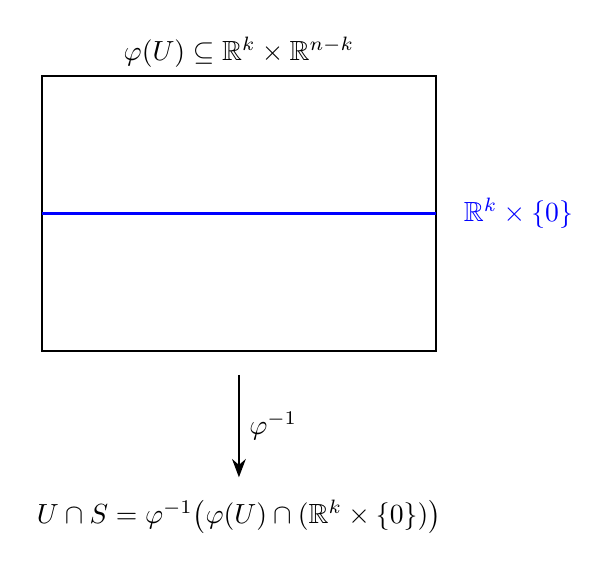
\begin{tikzpicture}[>=Stealth,scale=1]
\draw[thick] (0,0) rectangle (5,3.5);
\node at (2.5,3.8) {$\varphi(U)\subseteq\R^k\times\R^{n-k}$};
\draw[thick,blue] (0,1.75) -- (5,1.75);
\node[blue] at (6.05,1.75) {$\R^k\times\{0\}$};
\draw[->,thick] (2.5,-0.3) -- (2.5,-1.6) node[midway,right]{$\varphi^{-1}$};
\node at (2.5,-2.1) {$U\cap S=\varphi^{-1}\big(\varphi(U)\cap(\R^k\times\{0\})\big)$};
\end{tikzpicture}
\caption{Mapa plasterkowa: w mapie $\varphi$, przecięcie $U\cap S$ odpowiada dokładnie
przecięciu $\varphi(U)$ z podprzestrzenią $\R^k\times\{0\}$.}
\label{fig:plasterek}
\end{figure}

\begin{stwierdzenie}\label{stw:podrozm-struktura}
Jeśli $S\subseteq M$ jest podrozmaitością zanurzoną wymiaru $k$, to $S$ (z topologią
podprzestrzeni) jest rozmaitością topologiczną wymiaru $k$, posiadającą strukturę gładką,
względem której inkluzja $\iota\colon S\hookrightarrow M$ jest immersją; co więcej, $\iota$
jest zanurzeniem.
\end{stwierdzenie}
\begin{proof}
Wyposażamy $S$ w topologię podprzestrzeni. Ponieważ podprzestrzeń
przestrzeni Hausdorffa jest Hausdorffa, $S$ spełnia pierwszy warunek.
Jeśli $\mathcal B$ jest przeliczalną bazą $M$, to
$\{B\cap S:B\in\mathcal B\}$ jest przeliczalną bazą $S$:
dla otwartego $O\cap S$ i $p\in O\cap S$ znajdziemy
$B\in\mathcal B$ z $p\in B\subset O$, a wtedy
$p\in B\cap S\subset O\cap S$.

Ustalmy $p\in S$ i mapę plasterkową $(U,\varphi)$ przy $p$.
Ponieważ $U$ jest otwarte w $M$, zbiór $U_S=U\cap S$ jest otwarty
w $S$. Oznaczmy $W=\varphi(U)$, otwarty w $\R^n$.
Odwzorowanie $\varphi_S=\operatorname{pr}_1\circ\varphi|_{U_S}$
ma obraz $W_S=\{u\in\R^k:(u,0)\in W\}$, otwarty w $\R^k$ jako
przeciwobraz $W$ przez ciągłe zanurzenie $u\mapsto(u,0)$.
Odwrotność $u\mapsto\varphi^{-1}(u,0)$ jest ciągła; zatem
$\varphi_S:U_S\to W_S$ jest homeomorfizmem. To dowodzi lokalnej
euklidesowości $S$.

Niech teraz $(V,\psi)$ będzie drugą mapą plasterkową. Na
$\varphi_S(U\cap V\cap S)$ przejście ma wzór
\[
\psi_S\circ\varphi_S^{-1}(u)
=\operatorname{pr}_1\bigl((\psi\circ\varphi^{-1})(u,0)\bigr).
\]
Zanurzenie $u\mapsto(u,0)$, przejście $\psi\circ\varphi^{-1}$
i rzutowanie $\operatorname{pr}_1$ są gładkie, więc złożenie jest
gładkie. Zamieniając $\varphi$ i $\psi$, otrzymujemy gładką
odwrotność. Mapy $\varphi_S$ tworzą więc atlas gładki na $S$.

W mapach $\varphi_S$ i $\varphi$ inkluzja $\iota:S\to M$ ma postać
$u\mapsto(u,0)$, a jej różniczka wysyła $v$ na $(v,0)$ i jest
injektywna. Inkluzja jest więc immersją. Jako odwzorowanie
$S\to\iota(S)$ z \emph{topologią podprzestrzeni}, $\iota$ jest
homeomorfizmem już z wyboru topologii na $S$ (tożsamość na
zbiorze punktów). Zatem jest zanurzeniem.
\end{proof}

\begin{przyklad}[Wiązka normalna jako iloraz]
Niech $S\subset M$ będzie podrozmaitością zanurzoną. Poprzez różniczkę
inkluzji utożsamiamy $T_pS$ z podprzestrzenią $T_pM$. Wiązka $TS$ jest
podwiązką $TM|_S$. Włókna wiązki normalnej to ilorazy
\[
\nu_pS=T_pM/T_pS,\qquad \nu S=TM|_S/TS.
\]
Jej rząd wynosi $\dim M-\dim S$. W mapie plasterkowej
o współrzędnych $(x,y)$ klasa wektora stycznego
ma jednoznaczny reprezentant w kierunkach $\partial/\partial y^a$.
Sprawdźmy zmiany współrzędnych. Przejście między dwiema mapami
plasterkowymi ma postać $(x,y)\mapsto(a(x,y),b(x,y))$, przy czym
$b(x,0)=0$. Różniczkując tę tożsamość po $x$, dostajemy
$D_xb(x,0)=0$, więc różniczka przejścia na $S$ ma postać blokową
\[
 \begin{pmatrix} A&B\\0&C\end{pmatrix}.
\]
Cała macierz jest odwracalna, zatem kwadratowy blok $C$ jest
odwracalny. Klasa wektora o składowej poprzecznej $v$ zmienia
współrzędne na $Cv$, niezależnie od składowej stycznej.
Macierze $C$ są gładkie i spełniają warunek kocyklu, bo różniczki
przejść się składają. Twierdzenie o sklejaniu daje więc wiązkę
o zadanych włóknach ilorazowych. Konstrukcja jest kanoniczna bez metryki; po wybraniu
metryki można identyfikować klasy z wektorami prostopadłymi do $T_pS$.
\end{przyklad}

Poniższe twierdzenie i jego następstwa pokazują, w jaki sposób podrozmaitości powstają ,,w
praktyce'' — jako obrazy zanurzeń oraz jako przeciwobrazy wartości regularnych.

\begin{twierdzenie}[Twierdzenie o obrazie]\label{tw:obraz}
Jeśli $F\colon S\to M$ jest zanurzeniem ($\dim S=k\leq n=\dim M$), to $F(S)$ jest
podrozmaitością zanurzoną wymiaru $k$ w $M$, a $F\colon S\to F(S)$ (z topologią
podprzestrzeni) jest dyfeomorfizmem.
\end{twierdzenie}
\begin{proof}
Ustalmy $q=F(p_0)\in F(S)$. Ponieważ $F$ jest immersją w $p_0$, na mocy
Wniosku~\ref{wn:immersja-lokalnie} istnieją mapy $(U,\varphi)$ wokół $p_0$ w $S$ i
$(V,\psi)$ wokół $q$ w $M$, w których $F$ przyjmuje postać $u\mapsto(u,0)$.
Uzasadnijmy potrzebne dopasowanie dziedzin: wybieramy małe otwarte
kule $A\subset\R^k$, $B\subset\R^{n-k}$ o środku $0$, tak aby
$A\subset\varphi(U)$ i $A\times B\subset\psi(V)$.
Zastępujemy $U$ przez $\varphi^{-1}(A)$, a $V$ przez
$\psi^{-1}(A\times B)$. Wtedy rzeczywiście
$\psi(F(U))=A\times\{0\}=\psi(V)\cap(\R^k\times\{0\})$.
Zatem $(V,\psi)$ jest ,,prawie'' mapą
plasterkową dla $F(S)$, z tą różnicą, że warunek dotyczy $F(U)$, a nie od razu $F(S)\cap V$.

W tym miejscu wykorzystujemy założenie, że $F$ jest \emph{zanurzeniem}, nie tylko
różnowartościową immersją (por.\ Przykład~\ref{prz:osemka}): ponieważ $F\colon S\to F(S)$
jest homeomorfizmem na obraz, zbiór $F(U)$ jest otwarty w $F(S)$, tzn.\ $F(U)=F(S)\cap W$
dla pewnego otwartego $W\subseteq M$. Zastępując $V$ przez $V':=V\cap W$, otrzymujemy
$F(S)\cap V'=F(U)\cap V'$, a
\begin{align*}
\psi(F(S)\cap V')
 &=\psi(F(U)\cap V')\\
 &=\psi(F(U))\cap\psi(V')\\
 &=\big(\psi(V)\cap(\R^k\times\{0\})\big)\cap\psi(V')\\
 &=\psi(V')\cap(\R^k\times\{0\}).
\end{align*}
Zatem $(V',\psi|_{V'})$ jest mapą plasterkową rzędu $k$ dla $F(S)$ wokół $q$. Ponieważ
$q\in F(S)$ był dowolny, $F(S)$ jest podrozmaitością zanurzoną wymiaru $k$.

Wreszcie, $F\colon S\to F(S)$ jest bijekcją gładką (w mapach plasterkowych powyżej, $F$
przyjmuje postać identyczności), której odwrotność $F^{-1}\colon F(S)\to S$ jest gładka z
tego samego powodu. Zatem $F\colon S\to F(S)$ jest dyfeomorfizmem.
\end{proof}

\begin{definicja}
Niech $F\colon M\to N$ będzie gładkie, $q\in N$. Punkt $q$ jest \emph{wartością regularną}
$F$, jeśli dla każdego $p\in F^{-1}(q)$, $F$ jest submersją w $p$ (jeśli $F^{-1}(q)=
\emptyset$, $q$ jest — pusto — wartością regularną).
\end{definicja}

\begin{twierdzenie}[Twierdzenie o przeciwobrazie wartości regularnej]\label{tw:przeciwobraz}
Niech $F\colon M\to N$ będzie gładkie, $\dim M=m$, $\dim N=n$, i niech $q\in N$ będzie
wartością regularną $F$ z $F^{-1}(q)\neq\emptyset$. Wówczas $F^{-1}(q)$ jest
podrozmaitością zanurzoną wymiaru $m-n$ w $M$, a dla każdego $p\in F^{-1}(q)$,
\[
T_p\big(F^{-1}(q)\big)=\ker(dF_p)\subseteq T_pM.
\]
\end{twierdzenie}
\begin{proof}
Niech $p\in F^{-1}(q)$. Ponieważ $F$ jest submersją w $p$, na mocy
Wniosku~\ref{wn:submersja-lokalnie} istnieją mapy $(U,\varphi)$ wokół $p$ ($\varphi(p)=0$)
i $(V,\psi)$ wokół $q$ ($\psi(q)=0$), w których $F$ przyjmuje postać $\psi\circ F\circ
\varphi^{-1}(u^1,\dots,u^m)=(u^1,\dots,u^n)$. W tych mapach,
\[
\varphi(U\cap F^{-1}(q))=\{u\in\varphi(U):(u^1,\dots,u^n)=0\}=\varphi(U)\cap(\{0\}\times
\R^{m-n}).
\]
Po przenumerowaniu współrzędnych w $\R^m$ (zamiana miejscami pierwszych $n$ z pozostałymi
$m-n$), $(U,\varphi)$ staje się mapą plasterkową rzędu $m-n$ dla $F^{-1}(q)$ wokół $p$.
Ponieważ $p\in F^{-1}(q)$ był dowolny, $F^{-1}(q)$ jest podrozmaitością zanurzoną wymiaru
$m-n$.

W drugiej części niech $\iota\colon F^{-1}(q)\hookrightarrow M$
będzie inkluzją. Jest ona immersją na mocy
Stwierdzenia~\ref{stw:podrozm-struktura}. Ponieważ $F\circ\iota$ jest
odwzorowaniem stale równym $q$, jego różniczka znika: $dF_p\circ d\iota_p=0$ (reguła
łańcucha). Zatem $d\iota_p(T_pF^{-1}(q))\subseteq\ker(dF_p)$; utożsamiając (poprzez
injektywną immersję $d\iota_p$) $T_pF^{-1}(q)$ z jego obrazem w $T_pM$, mamy $T_pF^{-1}(q)
\subseteq\ker(dF_p)$. Z rachunku wymiarów: $\dim T_pF^{-1}(q)=m-n$ (z pierwszej części
dowodu), a $\dim\ker(dF_p)=m-\mathrm{rz}(dF_p)=m-n$ (bo $dF_p$ jest surjektywne na $T_qN$
wymiaru $n$, z definicji submersji). Zatem obie podprzestrzenie $T_pM$ mają ten sam,
skończony wymiar $m-n$, a jedna zawiera się w drugiej — więc są równe.
\end{proof}

\begin{wniosek}[Twierdzenie o poziomicy]
Jeśli $\dim M=n$, $f\colon M\to\R$ jest gładka, $c\in\R$ jest wartością regularną $f$ (tzn.\
$df_p\neq0$ dla każdego $p\in f^{-1}(c)$) i $f^{-1}(c)\neq\emptyset$, to $f^{-1}(c)$ jest
podrozmaitością zanurzoną wymiaru $n-1$ w $M$ (,,hiperpowierzchnią''), z $T_pf^{-1}(c)=
\ker(df_p)$.
\end{wniosek}
\begin{proof}
Szczególny przypadek Twierdzenia~\ref{tw:przeciwobraz} z $N=\R$: submersywność $f$ w
$p\in f^{-1}(c)$ to dokładnie warunek $df_p\neq0$.
\end{proof}

\begin{przyklad}
Niech $f\colon\R^{n+1}\to\R$, $f(x)=\|x\|^2$. Wtedy $df_x(v)=2\langle x,v\rangle$, niezerowe
dla $x\neq0$. Ponieważ $S^n=f^{-1}(1)$ i $0\notin f^{-1}(1)$, $1$ jest wartością regularną
— na mocy Wniosku powyżej, $S^n$ jest podrozmaitością zanurzoną wymiaru $n$ w $\R^{n+1}$
(zgodnie z tym, co wiedzieliśmy już z Przykładu~\ref{prz:sfera}; twierdzenie o poziomicy
daje jednak krótszy dowód gładkości struktury na $S^n$, choć nie podaje jawnych map).
\end{przyklad}

\begin{przyklad}[Grupa ortogonalna]
Niech $F\colon M_n(\R)\to\mathrm{Sym}(n)$, $F(A):=A^TA$, gdzie $\mathrm{Sym}(n)\cong
\R^{n(n+1)/2}$ oznacza przestrzeń macierzy symetrycznych. Różniczka: dla $H\in M_n(\R)$,
\[
dF_A(H)=\frac{d}{dt}\Big|_{t=0}(A+tH)^T(A+tH)=A^TH+H^TA.
\]
Dla $A\in\mathrm{O}(n):=F^{-1}(I)=\{A:A^TA=I\}$, $dF_A$ jest surjektywne na
$\mathrm{Sym}(n)$: dla symetrycznej $S$, kładąc $H:=\tfrac12AS$,
\[
dF_A(H)=A^T\big(\tfrac12AS\big)+\big(\tfrac12AS\big)^TA=\tfrac12(A^TA)S+\tfrac12S^TA^TA=
\tfrac12S+\tfrac12S=S
\]
(korzystając z $A^TA=I$, $S^T=S$). Zatem $I$ jest wartością regularną $F$, więc
$\mathrm{O}(n)=F^{-1}(I)$ jest podrozmaitością zanurzoną $M_n(\R)\cong\R^{n^2}$ wymiaru
$n^2-n(n+1)/2=n(n-1)/2$. Co więcej, $T_I\mathrm{O}(n)=\ker(dF_I)=\{H:H+H^T=0\}=:
\mathfrak{so}(n)$ — przestrzeń macierzy antysymetrycznych, wymiaru $n(n-1)/2$ (zgodnie z
powyższym rachunkiem wymiaru).
\end{przyklad}

\begin{uwaga}
Powyższy przykład jest pierwszym spotkaniem z fundamentalnym zjawiskiem: $\mathrm{O}(n)$
jest nie tylko rozmaitością, ale i grupą (względem mnożenia macierzy), w której mnożenie i
branie odwrotności są gładkie — tzw.\ \emph{grupą Liego} — a $T_I\mathrm{O}(n)=
\mathfrak{so}(n)$ jest jej \emph{algebrą Liego}.
\end{uwaga}

\begin{przyklad}[Torus jako regularna poziomica]
Niech $R>r>0$, $\rho=\sqrt{x^2+y^2}$ oraz
$\Omega=\{(x,y,z)\in\R^3:\rho>0\}$. Na tym otwartym zbiorze
$f(x,y,z)=(\rho-R)^2+z^2$ jest gładka. Poziom $f=r^2$
leży w $\Omega$, gdyż $|\rho-R|\leq r<R$ daje $\rho\geq R-r>0$.
Różniczka w punkcie $\Omega$ ma postać
\[
df=2(\rho-R)\left(\frac{x}{\rho}\,dx+
\frac{y}{\rho}\,dy\right)+2z\,dz.
\]
Jeżeli $df=0$, to $z=0$ oraz $\rho=R$: ponieważ $(x,y)\ne(0,0)$,
nie mogą jednocześnie znikać współczynniki przy $dx,dy$, chyba że
$\rho-R=0$. Lecz wtedy $f=0$, a więc taki punkt nie leży na
poziomie $r^2>0$. Zatem $r^2$ jest wartością regularną i torus
obrotowy $f^{-1}(r^2)$ jest gładką powierzchnią. Ponadto
$T_pT^2=\ker df_p$: wektor $(a,b,c)$ jest styczny wtedy i tylko
wtedy, gdy $(\rho-R)(xa+yb)/\rho+zc=0$.
\end{przyklad}
\clearpage

\chapter{Pola wektorowe, przepływy i pochodna Liego}
\label{ch:pola}
\index{pole wektorowe}

W Rozdziale~\ref{ch:rozmaitosci} zbudowaliśmy przestrzenie styczne i wiązkę $TM$.
Teraz wybieramy wektor \emph{w każdym} punkcie, w sposób gładki.
Otrzymujemy pole wektorowe: jednocześnie operator
różniczkowy, kierunek ruchu i infinitezymalny generator lokalnych dyfeomorfizmów.
Z tego jednego pojęcia wynikają nawias Liego, krzywe całkowe, przepływy oraz
pochodna Liego.

Rozdział rozwija rachunek pól oraz geometrię ich przepływów: najpierw
rozwiązujemy równanie krzywej całkowej, a następnie badamy ruch
punktów i sposób przenoszenia funkcji oraz pól wektorowych.
Do dalszej topologii różniczkowej przydadzą się zwłaszcza prostowanie
pola, pola zależne od czasu oraz rozszerzanie izotopii.
Przez $M$ rozumiemy rozmaitość gładką w sensie Definicji~\ref{def:rozmaitosc-gladka},
bez brzegu, chyba że wyraźnie zaznaczono inaczej.
Wszystkie pola i odwzorowania są klasy $C^\infty$.
Uwagi o brzegu i końcach przedziału czasu rozumiemy
według Definicji~\ref{def:rozmaitosc-z-brzegiem-1}
i opisu przestrzeni stycznej w
Sekcji~\ref{sec:rozmaitosci-z-brzegiem-1}.
Tak samo interpretujemy gładkie rodziny na domkniętym przedziale czasu.



\section{Pola wektorowe i derywacje globalne}
\label{sec:derywacje}

W Sekcji~\ref{sec:przestrzen-styczna} utożsamiliśmy wektor $v\in T_pM$ z
\emph{derywacją w punkcie} $v\colon C^\infty(M)\to\R$.
Teraz interesuje nas wybór takiej derywacji gładko w każdym
punkcie $p$. Jest to równoważne jednej derywacji, która każdej
funkcji gładkiej przypisuje \emph{funkcję} gładką.

\begin{definicja}
\emph{Pole wektorowe} $X$ na $M$ to gładki przekrój wiązki stycznej
$TM\to M$, czyli gładkie odwzorowanie $X\colon M\to TM$ spełniające
$X(p)\in T_pM$ dla każdego $p$. Przestrzeń pól oznaczamy $\X(M)=\Gamma(TM)$.
\end{definicja}

W mapie $(U;x^1,\ldots,x^n)$ pole zapisuje się jednoznacznie jako
\begin{equation}\label{eq:lokalne-pole}
 X\big|_U=\sum_{i=1}^{n}X^i\frac{\partial}{\partial x^i},
 \qquad X^i\in C^\infty(U).
\end{equation}
Współczynniki są gładkie; same wektory bazy zmieniają się przy zmianie mapy.
Przykładowo na $\R^2$ pole $X=-y\partial_x+x\partial_y$ jest w każdym punkcie
styczne do okręgu o środku w zerze. W zerze $X_0=0$.

\begin{definicja}
\emph{Derywacją} algebry $C^\infty(M)$ nazywamy $\R$-liniowe odwzorowanie
$D\colon C^\infty(M)\to C^\infty(M)$ spełniające regułę Leibniza
\[
 D(fg)=fD(g)+gD(f),\qquad f,g\in C^\infty(M).
\]
Zbiór takich derywacji oznaczamy $\operatorname{Der}_{\R}(C^\infty(M))$.
\end{definicja}

Pole $X$ działa na funkcje przez $D_X(f)(p):=X_p(f)$.
Współrzędnie $D_X(f)=\sum_iX^i\partial_if$, więc
$D_X$ jest derywacją globalną. Odwrotnie, dla derywacji
globalnej $D$ wartość $v_p(f):=D(f)(p)$ jest liczbą
i spełnia \emph{punktową} regułę Leibniza:
\[
 v_p(fg)=f(p)v_p(g)+g(p)v_p(f).
\]
Zatem $v_p\in T_pM$. Lemat~\ref{lem:lokalnosc} mówi w szczególności,
że $D(f)(p)$ zależy tylko od kiełka $f$ w $p$.
Rozróżniajmy więc $v_p\colon C^\infty(M)\to\R$
oraz $D\colon C^\infty(M)\to C^\infty(M)$.

\begin{twierdzenie}\label{thm:derywacje-pola}
Odwzorowanie
\[
 \X(M)\longrightarrow\operatorname{Der}_{\R}(C^\infty(M)),
 \qquad X\longmapsto(f\longmapsto X(f))
\]
jest izomorfizmem $C^\infty(M)$-modułów.
\end{twierdzenie}
\begin{proof}
Niech $D$ będzie derywacją globalną. Z poprzedniego
rachunku $X_p:=v_p$ jest wektorem stycznym w każdym $p$.
Pozostaje sprawdzić, że $p\mapsto X_p$ jest gładkie.
Wybierzmy wokół dowolnego punktu mapę $(U;x^1,\ldots,x^n)$
i mniejsze otoczenie $V$, którego obraz jest kulą o domknięciu
zawartym w obrazie mapy.
Funkcja odcinająca $\chi$ równa $1$ na $V$
i wsparta w $U$ pozwala przedłużyć każdą współrzędną
do funkcji $\widetilde x^i=\chi x^i\in C^\infty(M)$
(poza $U$ kładziemy ją równą zeru). Dla $p\in V$
lokalność derywacji punktowej daje
\[
 X_p=\sum_i X^i(p)\,\partial_i\big|_p,
 \qquad X^i(p)=v_p(\widetilde x^i)=D(\widetilde x^i)(p).
\]
Każda funkcja $D(\widetilde x^i)$ jest gładka z definicji
derywacji globalnej. Zbiory $V$ pokrywają $M$, zatem
$X$ jest polem gładkim. W drugą stronę gładkie pole $X$
daje derywację $D_X$ przez lokalny wzór
$D_X(f)=\sum_iX^i\partial_if$ i regułę Leibniza.
Obie konstrukcje są odwrotne, a
$D_{fX}=fD_X$ dla $f\in C^\infty(M)$.
\end{proof}

\begin{uwaga}[Dlaczego to jest moduł, a nie zwykle przestrzeń z bazą]
Przestrzeń $\X(M)$ jest modułem nad pierścieniem funkcji: $(fX)_p=f(p)X_p$.
Nie musi mieć jednej globalnej bazy nad $C^\infty(M)$. Na przykład
$TS^2$ nie jest wiązką trywialną; nie da się wybrać dwóch globalnych,
wszędzie liniowo niezależnych pól na sferze. Lokalne bazy
$\partial_{x^1},\ldots,\partial_{x^n}$ zawsze istnieją.
Używamy tu klasycznego twierdzenia o nieistnieniu nigdzie
niezerowego pola na $S^2$; wynika ono również z późniejszego
Twierdzenia~\ref{thm:poincare-hopf-16} i $\chi(S^2)=2$.
\end{uwaga}

\begin{przyklad}[Pole na sferze]
Na $S^2\subset\R^3$ weźmy $X(x,y,z)=(-y,x,0)$.
Iloczyn skalarny $X(x,y,z)\cdot(x,y,z)=0$, zatem $X$ jest styczne
w każdym punkcie. Ma zera na biegunach; poza nimi wskazuje kierunek
obrotu wokół osi $z$. Jest to pole globalne, choć współrzędna kątowa
nie jest globalną mapą na sferze.
\end{przyklad}

\begin{uwaga}[Pole wzdłuż odwzorowania]
Dla gładkiego $F\colon M\to N$ i $X\in\X(M)$ wektory
$\dd F_p(X_p)$ tworzą \emph{pole wzdłuż $F$}.
Precyzyjnie, jest to przekrój wiązki cofniętej
\[
 F^*TN=\{(p,v):p\in M,\ v\in T_{F(p)}N\}\longrightarrow M,
 \qquad(p,v)\longmapsto p.
\]
Mapy na $N$ dają jej lokalne trywializacje nad ich przeciwobrazami
przez $F$; współczynniki przejść są gładkie, bo są złożeniami
przejść $TN$ z $F$. Dla ogólnego $F$ różne punkty $p$ nad jednym
$q=F(p)$ mogą dawać różne wektory, a punkty poza $F(M)$ nie dostają
żadnej wartości. Gdy $F$ jest dyfeomorfizmem, otrzymujemy pole
\[
 (F_*X)_q=\dd F_{F^{-1}(q)}X_{F^{-1}(q)}.
\]
Bardziej ogólnie pole na $N$ może istnieć przy dodatkowej zgodności
wektorów na włóknach $F$, ale nie jest dane automatycznie.
\end{uwaga}

\section{Nawias Liego: mierzenie nieprzemienności}
\label{sec:nawias}

Dwa pola są operatorami na funkcjach. Można je więc składać i wziąć
ich komutator.
\begin{definicja}
\emph{Nawiasem Liego} pól $X,Y\in\X(M)$ nazywamy pole $[X,Y]$ zadane przez
\begin{equation}\label{eq:nawias-def}
 [X,Y](f)=X(Y(f))-Y(X(f)),\qquad f\in C^\infty(M).
\end{equation}
\end{definicja}

Choć $X\circ Y$ jako operator jest na ogół drugiego rzędu, wyrazy z
pochodnymi drugimi znoszą się w różnicy.
\begin{fakt}\label{fakt:nawias-wlasnosci}
$[X,Y]$ jest polem wektorowym. Ponadto nawias jest dwuliniowy nad $\R$,
antysymetryczny i spełnia tożsamość Jacobiego
\[
 [X,[Y,Z]]+[Y,[Z,X]]+[Z,[X,Y]]=0.
\]
Jego reguła Leibniza względem funkcji ma postać
\begin{equation}\label{eq:nawias-leibniz}
 [X,fY]=f[X,Y]+X(f)Y,\qquad [fX,Y]=f[X,Y]-Y(f)X.
\end{equation}
\end{fakt}
\begin{proof}
Pokażmy najpierw, że komutator jest derywacją, choć samo
złożenie dwóch derywacji nią zazwyczaj nie jest.
Dla funkcji $f,g$ dwukrotnie stosujemy regułę Leibniza:
\begin{align*}
[X,Y](fg)
&=X\bigl(Y(f)g+fY(g)\bigr)
  -Y\bigl(X(f)g+fX(g)\bigr)\\
&=X(Yf)g+Y(f)X(g)+X(f)Y(g)+fX(Yg)\\
&\quad-Y(Xf)g-X(f)Y(g)-Y(f)X(g)-fY(Xg)\\
&=[X,Y](f)g+f[X,Y](g).
\end{align*}
Wyrazy mieszane znoszą się dokładnie parami. Komutator
jest liniowy nad $\R$ i spełnia regułę Leibniza,
więc z Twierdzenia~\ref{thm:derywacje-pola} odpowiada
gładkiemu polu wektorowemu. Z definicji natychmiast
$[X,Y]=-[Y,X]$; liniowość w obu argumentach wynika
z liniowości składania operatorów.

Sprawdźmy tożsamość Jacobiego, pokazując wszystkie
wyrazy. Jako operatory na funkcjach mamy
\begin{align*}
[X,[Y,Z]]&=XYZ-XZY-YZX+ZYX,\\
[Y,[Z,X]]&=YZX-YXZ-ZXY+XZY,\\
[Z,[X,Y]]&=ZXY-ZYX-XYZ+YXZ.
\end{align*}
Suma prawych stron jest zerowa: np.\ $XYZ$ znosi się
z $-XYZ$, a analogicznie pozostałe pięć możliwych
kolejności. Ponieważ równość operatorów zachodzi na
każdej funkcji, zachodzi równość pól wektorowych.

Na koniec stosujemy definicję do dowolnej funkcji $g$:
\begin{align*}
[X,fY](g)
 &=X\bigl(fY(g)\bigr)-fY\bigl(X(g)\bigr)
  =X(f)Y(g)+f[X,Y](g),\\
[fX,Y](g)
 &=fX\bigl(Y(g)\bigr)-Y\bigl(fX(g)\bigr)
  =f[X,Y](g)-Y(f)X(g).
\end{align*}
Funkcje rozróżniają pola, zatem są to dokładnie
równości~\eqref{eq:nawias-leibniz}.
\end{proof}

W mapie, jeśli $X=X^i\partial_i$ i $Y=Y^j\partial_j$, to
\begin{equation}\label{eq:nawias-wspolrzedne}
 [X,Y]=\sum_{j=1}^{n}\left(\sum_{i=1}^{n}
 X^i\frac{\partial Y^j}{\partial x^i}-
 Y^i\frac{\partial X^j}{\partial x^i}\right)\partial_j.
\end{equation}
Istotnie, współczynnik przy $\partial_j$ jest równy
$[X,Y](x^j)=X(Y^j)-Y(X^j)$; na funkcjach lokalnych możemy
działać dzięki lokalności derywacji. Tu i dalej $\partial_i$
skraca $\partial/\partial x^i$, a powtórzony indeks w zapisie
takim jak $X^i\partial_i$ oznacza sumowanie po tym indeksie.
Ważny wniosek: $[\partial_i,\partial_j]=0$ w układzie współrzędnych,
ale ogólne pola bazowe, np.\ ramy ruchome, nie muszą komutować.

\begin{przyklad}[Ścinanie płaszczyzny]\label{prz:scinanie}
Niech $X=\partial_x$ i $Y=x\partial_y$ na $\R^2$.
Wtedy $[X,Y]=\partial_y$. Najpierw przesunięcie w kierunku $x$
zmienia prędkość pionową $Y$; wykonanie ruchów w odwrotnej kolejności
daje inny wynik. Pole $Y$ ma zera na osi $x=0$ i nie jest polem
przesunięcia o stałej prędkości.
\end{przyklad}

\begin{przyklad}[Obrót i skalowanie]
Dla $R=-y\partial_x+x\partial_y$ i $E=x\partial_x+y\partial_y$
na $\R^2$ mamy $[R,E]=0$. Obrót i jednolite powiększenie
można wykonywać w dowolnej kolejności. Jeśli zaś
$X=\partial_x$, $Y=x\partial_y$, to wynik jest niezerowy
mimo że w punkcie $(0,0)$ mamy $Y=0$; nawias uwzględnia zmienność
pola w otoczeniu punktu.
\end{przyklad}



\begin{uwaga}[Rozkłady styczne i twierdzenie Frobeniusa]
Rozkładem gładkim stałego rzędu $k$ nazywamy podwiązkę
$\mathcal D\subset TM$, lokalnie rozpiętą przez $k$ gładkich,
punktowo liniowo niezależnych pól. Jest \emph{inwolutywny}, jeśli
$[X,Y]$ jest sekcją $\mathcal D$, gdy $X,Y$ są jej sekcjami.
Twierdzenie Frobeniusa mówi, że dokładnie wtedy lokalnie
istnieją współrzędne $(u^1,\ldots,u^n)$, w których
$\mathcal D=\operatorname{span}(\partial_{u^1},\ldots,\partial_{u^k})$.
Plasterki o stałych $u^{k+1},\ldots,u^n$ są wtedy lokalnymi
podrozmaitościami całkowymi (fragmentami \emph{liści}).
Przykład przeciwny na $\R^3$:
\[
 \mathcal D
 =\operatorname{span}\{\partial_x,\partial_y+x\partial_z\}.
\]
Nawias generatorów jest równy $\partial_z$, który nie należy do $\mathcal D$.
Nie ma zatem powierzchni, których przestrzenie styczne pokrywałyby się
z tym rozkładem. Konieczność warunku jest widoczna już w mapie
plasterkowej: składowe normalne pól stycznych znikają na
podrozmaitości, więc ich pochodne w kierunkach stycznych również
tam znikają; wzór~\eqref{eq:nawias-wspolrzedne} pokazuje,
że nawias jest styczny. W przykładzie $\partial_z$ nie jest
kombinacją generatorów: składowe $x,y$ wymusiłyby zerowe
współczynniki. Dowód dostateczności podamy po twierdzeniu
o prostowaniu pola, w Stwierdzeniu~\ref{prop:frobenius-lokalny}.
\end{uwaga}

\section{Krzywe całkowe i równania różniczkowe na rozmaitości}
\label{sec:krzywe}

\begin{definicja}
\emph{Krzywą całkową} pola $X$ nazywamy krzywą
$\gamma\colon I\to M$ na otwartym przedziale $I\subset\R$ spełniającą
\begin{equation}\label{eq:krzywa-calkowa}
 \gamma'(t)=X_{\gamma(t)}.
\end{equation}
Jeśli $0\in I$ i $\gamma(0)=p$, mówimy o krzywej wychodzącej z $p$.
Jest \emph{maksymalna}, gdy nie daje się przedłużyć jako rozwiązanie
na większy przedział.
\end{definicja}

Współrzędnie, dla $\gamma(t)=(x^1(t),\ldots,x^n(t))$,
warunek~\eqref{eq:krzywa-calkowa} staje się układem równań
różniczkowych zwyczajnych (ODE)
\[
 \frac{\dd x^i}{\dd t}=X^i(x^1(t),\ldots,x^n(t)),\qquad i=1,\ldots,n.
\]
Krzywa nie musi być prostą nawet wtedy, gdy wektory pola rysujemy
jako małe strzałki. W każdym swoim punkcie porusza się w kierunku
aktualnej strzałki; prędkość także jest przez nią określona.

\begin{twierdzenie}[Istnienie, jednoznaczność i zależność od danych]
\label{thm:ode}
Dla każdego $p\in M$ istnieje dokładnie jedna maksymalna krzywa
całkowa $\gamma_p\colon I_p\to M$ pola $X$, gdzie $I_p$ jest otwartym
przedziałem zawierającym $0$ i $\gamma_p(0)=p$.
Rozwiązania zależą gładko od czasu i punktu początkowego tam,
gdzie są określone.
\end{twierdzenie}
\begin{proof}
\emph{Krok 1: konstrukcja w mapie.}
Wybierzmy mapę wokół $p$ i oznaczmy przez $u_0$ współrzędne punktu
$p$. Równanie~\eqref{eq:krzywa-calkowa} przyjmuje postać
$u'(t)=F(u(t))$, gdzie $F$ jest gładkim odwzorowaniem
otwartego zbioru w $\R^n$ do $\R^n$.
Wybierzmy $r>0$ tak, aby domknięta kula
$\overline B_{2r}(u_0)$ leżała w dziedzinie mapy.
Na tej kuli istnieją stałe $A,L\geq 0$ spełniające
$\|F(u)\|\leq A$ oraz $\|\D F(u)\|\leq L$.
Twierdzenie o wartości średniej daje
$\|F(u)-F(v)\|\leq L\|u-v\|$ dla punktów tej kuli.
Wybierzmy $h>0$ tak, aby $hA<r$ i $hL<1$
(gdy $A=0$ lub $L=0$, odpowiedni warunek jest automatyczny).

Dla każdego warunku początkowego $a\in B_r(u_0)$ rozważmy
zupełną przestrzeń krzywych ciągłych
$z\colon[-h,h]\to\overline B_{2r}(u_0)$ z normą supremum.
Operator Picarda
\[
 (\mathcal T_a z)(t)=a+\int_0^t F(z(\tau))\,\dd\tau
\]
odwzorowuje ją w siebie, ponieważ
$\|\mathcal T_a z(t)-u_0\|<r+hA<2r$.
Ponadto
$\|\mathcal T_a z-\mathcal T_a w\|_\infty
 \leq hL\|z-w\|_\infty$.
Z twierdzenia Banacha o punkcie stałym otrzymujemy jedną
krzywą $z_a$ spełniającą równanie całkowe, a po zróżniczkowaniu
$z_a'(t)=F(z_a(t))$. Jest ona gładka w czasie, bo $F$ jest gładkie.

\emph{Krok 2: zależność od punktu początkowego.}
Z równań całkowych dla $z_a$ i $z_b$ oraz z oszacowania
kontrakcji otrzymujemy
\[
 \|z_a-z_b\|_\infty
 \leq \|a-b\|+hL\|z_a-z_b\|_\infty,
 \qquad
 \|z_a-z_b\|_\infty\leq\frac{\|a-b\|}{1-hL}.
\]
To dowodzi najpierw ciągłej zależności, jednak do gładkości
potrzeba więcej. Dla ustalonego $a$ rozwiążmy liniowe
równanie całkowe dla macierzy $J_a(t)$:
\[
 J_a(t)=I+\int_0^t\D F(z_a(\tau))J_a(\tau)\,\dd\tau.
\]
Operator po prawej, działający na ciągłe funkcje o wartościach
macierzowych, również ma stałą kontrakcji $hL<1$.
Istnieje więc jedyne $J_a$; spełnia ono równanie
wariacyjne $J_a'=\D F(z_a)J_a$, $J_a(0)=I$.

Sprawdźmy, że jest to rzeczywiście pochodna względem $a$.
Niech $v$ będzie małe, $\delta=z_{a+v}-z_a$.
Ponieważ $\D^2F$ jest ograniczona na $\overline B_{2r}(u_0)$,
rozwinięcie Taylora na odcinku między $z_a(\tau)$
a $z_{a+v}(\tau)$ daje, z pewną stałą $C$ niezależną
od $v$ i $\tau$,
\[
 \|F(z_a(\tau)+\delta(\tau))-F(z_a(\tau))
       -\D F(z_a(\tau))\delta(\tau)\|
 \leq C\|\delta\|_\infty^2.
\]
Odejmujemy równania całkowe dla $z_{a+v}$, $z_a$
i $J_av$. Dla $R=z_{a+v}-z_a-J_av$ dostajemy
\[
 \|R\|_\infty
 \leq hL\|R\|_\infty+hC\|\delta\|_\infty^2
 \leq hL\|R\|_\infty+
       \frac{hC}{(1-hL)^2}\|v\|^2.
\]
Zatem $\|R\|_\infty=O(\|v\|^2)$ i
$\D_a z_a(t)=J_a(t)$. Dla ciągłości tej pochodnej zauważmy,
że $\|J_a\|_\infty\leq(1-hL)^{-1}$ oraz
\[
 \|J_a-J_b\|_\infty
 \leq\frac{h}{(1-hL)^2}
 \|\D F(z_a)-\D F(z_b)\|_\infty.
\]
Prawa strona dąży do zera dla $b\to a$, dzięki ciągłości
$a\mapsto z_a$ i jednostajnej ciągłości $\D F$ na zwartej kuli.
Dalsze pochodne otrzymujemy w ten sam sposób, ale trzeba
odróżnić ich konstrukcję od formalnego różniczkowania.
Na przykład kandydat na drugą pochodną
$H_a(t)[v,w]$ spełnia
\[
 H_a(t)[v,w]=\int_0^t\bigl(
 \D F(z_a)H_a[v,w]
 +\D^2F(z_a)[J_av,J_aw]\bigr)(\tau)\,\dd\tau.
\]
Najpierw rozwiązujemy to liniowe równanie całkowe dla $H_a$.
Następnie odejmujemy równania dla $J_{a+v}$ i $J_a$ oraz
kandydata $H_a[v,\cdot]$. Wzór Taylora dla $\D F$ i
już dowiedziona różniczkowalność $z_a$ dają dla reszty
oszacowanie $\|R\|_\infty\leq hL\|R\|_\infty+o(\|v\|)$,
a więc $H_a=\D_aJ_a$.
Ogólnie, po $k$ różniczkowaniach złożenia $F(z_a)$
jedynym wyrazem zawierającym nieznaną $k$-tą pochodną $Z_k$
jest $\D F(z_a)Z_k$. Wszystkie pozostałe wyrazy są sumami
iloczynów pochodnych $F$ i już skonstruowanych pochodnych
$Z_j$ z $j<k$. Wyznaczają więc znane ciągłe wymuszenie.
Równanie dla $Z_k$ ma ponownie stałą kontrakcji $hL<1$;
porównanie równań dla $Z_{k-1}(a+v)$ i $Z_{k-1}(a)$
z wzorem Taylora daje tę samą resztę $o(\|v\|)$.
Indukcyjnie dowodzi to istnienia wszystkich pochodnych,
a porównanie równań przy $a,b$ --- ich ciągłości.
Równanie $z_a'=F(z_a)$ zapewnia również ciągłość
pochodnych mieszanych po $t$ i $a$. Otrzymujemy
gładkość $(t,a)\mapsto z_a(t)$.

\emph{Krok 3: przedział maksymalny.}
Dwie krzywe całkowe wychodzące z $p$ są równe w pobliżu zera
na mocy powyższej jednoznaczności. Zbiór czasów, w których
się zgadzają, jest domknięty w części wspólnej ich
przedziałów przez ciągłość obu krzywych. Jest też otwarty:
w punkcie, w którym się zgadzają, stosujemy lokalną
jednoznaczność ponownie. Ponieważ część wspólna jest przedziałem,
krzywe pokrywają się wszędzie, gdzie obie są określone.
Można więc skleić wszystkie rozwiązania przez $p$ na sumie
ich przedziałów. Suma ta jest otwartym przedziałem $I_p$
zawierającym zero; sklejenie daje rozwiązanie, którego żadne
dalsze przedłużenie nie istnieje. Jednoznaczność w mapach
zapewnia, że konstrukcja nie zależy od wyboru współrzędnych.
Gładkość przy innych chwilach niż zero uzyskujemy, zaczynając
lokalny argument od dowolnego punktu tej krzywej; szczegóły
otwartości wspólnej dziedziny podajemy w dowodzie
Twierdzenia~\ref{thm:przeplyw}.
\end{proof}

Jeśli $X_p=0$, to jedyną krzywą wychodzącą z $p$ jest krzywa stała.
Jeśli dwie krzywe całkowe spotkają się, to po odpowiednim przesunięciu
parametru czasu pokrywają się tam, gdzie obie są określone.
Mogą więc tworzyć orbitę okresową, lecz nie mogą przecinać się
transwersalnie jako trajektorie tego samego pola.

\begin{przyklad}[Obrót]
Na $\R^2$ niech $X=-y\partial_x+x\partial_y$. Układ
$x'=-y$, $y'=x$ daje
\begin{equation}\label{eq:obrot}
 \gamma_{(a,b)}(t)=(a\cos t-b\sin t,\ a\sin t+b\cos t).
\end{equation}
Dla $(a,b)\ne(0,0)$ trajektorią jest okrąg o promieniu
$\sqrt{a^2+b^2}$, przebiegany przeciwnie do ruchu wskazówek zegara.
Początek układu jest punktem stałym.
\end{przyklad}

\begin{figure}[!htbp]
\centering
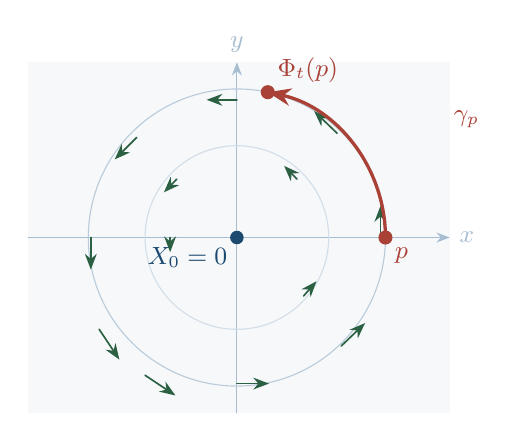
\begin{tikzpicture}[>=Stealth,scale=1.06,line cap=round]
\fill[manifoldblue!4] (-2.5,-2.1) rectangle (2.55,2.1);
\draw[->,manifoldblue!40] (-2.5,0)--(2.55,0) node[right,font=\small] {$x$};
\draw[->,manifoldblue!40] (0,-2.1)--(0,2.1) node[above,font=\small] {$y$};
\draw[manifoldblue!20] (0,0) circle (1.1);
\draw[manifoldblue!32] (0,0) circle (1.78);
\foreach \xx/\yy in {-1.65/-1.1,-1.1/-1.65,0/-1.75,1.25/-1.3,1.72/0,
 1.2/1.25,0/1.65,-1.2/1.2,-1.75/0,-.8/0,.72/.7,-.72/.7,.8/-.7}{
 \draw[->,manifoldgreen!78!black,semithick]
 (\xx,\yy)--++({-.22*\yy},{.22*\xx});}
\draw[manifoldred,very thick,->] (1.78,0)
 arc[start angle=0,end angle=78,radius=1.78];
\fill[manifoldred] (1.78,0) circle (2.4pt)
 node[below right,font=\small] {$p$};
\fill[manifoldred] ({1.78*cos(78)},{1.78*sin(78)}) circle (2.4pt)
 node[above right,font=\small] {$\Phi_t(p)$};
\fill[manifoldblue!80!black] (0,0) circle (2.3pt)
 node[below left,font=\small] {$X_0=0$};
\node[font=\small,manifoldred] at (2.75,1.42) {$\gamma_p$};
\end{tikzpicture}
\caption{Pole obrotowe $X=(-y,x)$: zielone strzałki przedstawiają wartości
pola pomniejszone wspólnym czynnikiem $0.22$,
a czerwona krzywa jest jego krzywą całkową. Strzałka pola
w każdym punkcie jest styczna do trajektorii.}
\label{fig:obrot-krzywa}
\end{figure}

\begin{przyklad}[Zmiana prędkości bez zmiany orbit]
Jeżeli $Y=fX$, gdzie $f>0$, to $X$ i $Y$ wyznaczają te same
\emph{zorientowane ślady} krzywych całkowych, choć czas ich
przebiegania jest inny. Gdy $f$ zmienia znak, orientacja ruchu może się
zmienić; gdy znika, pojawiają się punkty stałe. Dlatego sam obraz
krzywych nie wyznacza pola ani jego przepływu.
Dokładniej, jeśli $\gamma:I\to M$ jest krzywą $X$ z $\gamma(0)=p$,
to funkcja
\[
 s(\tau)=\int_0^\tau\frac{du}{f(\gamma(u))}
\]
ma dodatnią pochodną i jest dyfeomorfizmem $I$ na pewien
przedział $J$. Dla odwrotności $\tau=\tau(s)$ krzywa
$\eta(s)=\gamma(\tau(s))$ spełnia
$\eta'=f(\eta)X_\eta=Y_\eta$. Ta sama konstrukcja z $X=Y/f$
pokazuje równość orbit maksymalnych. Dokładniej, gdyby $\eta$
dała się przedłużyć przez skończony koniec $J$, równanie
$\tau'(s)=f(\eta(s))$ dawałoby tam skończoną wartość $\tau$
i dodatnią pochodną. Odwrotna zmiana czasu przedłużyłaby wtedy
$\gamma$ przez koniec $I$, wbrew jej maksymalności.
Przedziały czasu mogą
jednak być różne: zupełne $X=\partial_x$ po pomnożeniu przez
$f(x)=1+x^2$ daje niezupełne pole z krzywą $\tan s$ przez zero.
\end{przyklad}

\section{Przepływ lokalny, maksymalny i zupełny}
\label{sec:przeplyw}

Krzywe całkowe dla wszystkich punktów początkowych łączą się
w jedno odwzorowanie. W czasie $t$ przesuwamy punkt o tyle, ile
pozwala równanie~\eqref{eq:krzywa-calkowa}.

\begin{definicja}
Niech $\gamma_p\colon I_p\to M$ będzie maksymalną krzywą całkową.
\emph{Dziedziną maksymalnego przepływu} jest zbiór
$\mathcal D_X=\{(t,p)\in\R\times M:t\in I_p\}$, a
\emph{przepływem} pola $X$ odwzorowanie
\[
 \Phi\colon\mathcal D_X\to M,\qquad \Phi(t,p)=\Phi_t(p):=\gamma_p(t).
\]
Pole jest \emph{zupełne}, jeśli $\mathcal D_X=\R\times M$.
\end{definicja}

\begin{twierdzenie}[Podstawowe własności przepływu]
\label{thm:przeplyw}
Zbiór $\mathcal D_X$ jest otwarty, a $\Phi$ jest gładki. Zachodzi
\[
 \Phi_0=\id_M,\qquad
 \Phi_{t+s}(p)=\Phi_t(\Phi_s(p))
\]
dokładnie dla $s\in I_p$ i $t\in I_{\Phi_s(p)}$; przy tym
$I_{\Phi_s(p)}=I_p-s$. Dla $M_t:=\{p\in M:t\in I_p\}$
odwzorowania $\Phi_t\colon M_t\to M_{-t}$ i $\Phi_{-t}$ są wzajemnie
odwrotnymi dyfeomorfizmami między otwartymi zbiorami. Ponadto
\begin{equation}\label{eq:przeplyw-generuje}
 \left.\frac{\dd}{\dd t}\right|_{t=0}\Phi_t(p)=X_p,
 \qquad (\dd\Phi_t)_pX_p=X_{\Phi_t(p)}.
\end{equation}
Jeśli $X$ jest zupełne, $(\Phi_t)_{t\in\R}$ jest jednoparametrową
grupą dyfeomorfizmów.
\end{twierdzenie}
\begin{proof}
\emph{Otwartość i gładkość.}
Krok 1 poprzedniego dowodu daje dla każdego $q\in M$
otoczenie $W_q$ i liczbę $\varepsilon_q>0$, wspólną
dla punktów początkowych z $W_q$, na której lokalne
rozwiązanie istnieje i jest gładkie względem $(u,x)$.
Ustalmy $(t_0,p_0)\in\mathcal D_X$; rozważmy najpierw
$t_0>0$. Krzywa $\gamma_{p_0}$ jest określona
na pewnym otwartym przedziale obejmującym $[0,t_0]$.
Jej obraz $K=\gamma_{p_0}([0,t_0])$ jest zwarty.
Z pokrycia $K$ przez otwarte zbiory $W_q$ wybierzmy
skończone podpokrycie $W_{q_1},\ldots,W_{q_m}$.
Liczba $\varepsilon=\min_i\varepsilon_{q_i}$ jest dodatnia:
z każdego punktu $K$ można rozpocząć lokalne
rozwiązanie przez czas co najmniej $\varepsilon$.
Podzielmy odcinek czasu na
\[
 0=\tau_0<\tau_1<\cdots<\tau_N=t_0
\]
o długościach $\tau_{j+1}-\tau_j<\varepsilon/2$.
Każdy krok wzdłuż $\gamma_{p_0}$ jest wtedy
fragmentem lokalnego rozwiązania z jednego $W_{q_i}$.

Dla $j=0$ lokalny przepływ o czas
$\tau_1-\tau_0$ jest określony i gładki na pewnym
otoczeniu $p_0$. Jego obraz punktu $p_0$ to
$\gamma_{p_0}(\tau_1)$. Ciągłość pozwala zmniejszyć
otoczenie tak, by obrazy pobliskich punktów
należały do dziedziny następnego kroku. Powtarzając
ten argument skończenie wiele razy, otrzymujemy
otoczenie $V$ punktu $p_0$, na którym
$p\mapsto\Phi_{t_0}(p)$ jest gładkim złożeniem
lokalnych rozwiązań. W otoczeniu punktu
$\Phi_{t_0}(p_0)$ można prowadzić rozwiązanie
jeszcze przez wspólny krótki czas $u$.
Po ewentualnym zmniejszeniu $V$ wzór
\[
 \Phi_{t_0+u}(p)
 =\Phi_u\bigl(\Phi_{t_0}(p)\bigr)
\]
wynika z jednoznaczności i definiuje gładkie odwzorowanie
dla $(u,p)$ bliskich $(0,p_0)$. To samo rozumowanie
działa dla $t_0<0$, idąc po krzywej wstecz; przy
$t_0=0$ wystarcza konstrukcja lokalna.
W konsekwencji każde $(t_0,p_0)\in\mathcal D_X$
ma otoczenie zawarte w $\mathcal D_X$, na którym
$\Phi$ jest gładkie. Dowodzi to zarazem otwartości
dziedziny i gładkości przepływu.

\emph{Przesunięcie czasu i prawo grupowe.}
Niech $s\in I_p$ i $q=\Phi_s(p)$. Krzywa
$u\mapsto\gamma_p(s+u)$, określona na $I_p-s$, jest
rozwiązaniem wychodzącym z $q$, więc z jednoznaczności
$I_p-s\subset I_q$. W szczególności $-s\in I_q$.
Krzywa $v\mapsto\gamma_q(v-s)$, określona na $s+I_q$,
jest rozwiązaniem przez $p$ w chwili $v=0$.
Maksymalność $\gamma_p$ daje $s+I_q\subset I_p$.
Oba zawierania dowodzą $I_q=I_p-s$ i
\[
 \Phi_u(q)=\gamma_q(u)=\gamma_p(s+u)=\Phi_{s+u}(p)
 \quad\text{dla każdego }u\in I_q.
\]
Gdy $s\in I_p$, warunki $u\in I_q$ i $s+u\in I_p$
są więc równoważne. Zatem równość składania
obowiązuje dokładnie przy warunkach podanych w tezie.
Szczególny przypadek $s=0$ daje
$\Phi_0(p)=p$.

\emph{Odwrotności i generator.}
Ponieważ $\mathcal D_X$ jest otwarty, każdy $M_t$ jest otwarty.
Jeśli $q=\Phi_t(p)$, to $-t\in I_q$ i prawo składania
daje $\Phi_{-t}(q)=p$. Ten sam argument z zamienionymi
$t$ i $-t$ pokazuje, że $\Phi_t(M_t)=M_{-t}$;
gładkość obu odwzorowań daje dyfeomorfizm.
Pierwszy wzór w~\eqref{eq:przeplyw-generuje} jest równaniem
krzywej całkowej w chwili zero. Dla drugiego różniczkujemy
względem $s$ w zerze równość
$\Phi_t(\Phi_s(p))=\Phi_s(\Phi_t(p))$.
Po lewej stronie reguła łańcucha daje
$(\dd\Phi_t)_pX_p$, po prawej $X_{\Phi_t(p)}$.

Jeżeli $X$ jest zupełne, $M_t=M$ dla każdego $t$.
Wtedy wszystkie $\Phi_t$ są dyfeomorfizmami całej
rozmaitości i
$\Phi_{t+s}=\Phi_t\circ\Phi_s$, $\Phi_0=\id_M$,
$\Phi_t^{-1}=\Phi_{-t}$. Składanie dyfeomorfizmów
jest łączne, a wzór na parametry daje wprost
$\Phi_r\circ(\Phi_s\circ\Phi_t)=\Phi_{r+s+t}
=(\Phi_r\circ\Phi_s)\circ\Phi_t$.
Odwzorowanie $t\mapsto\Phi_t$ jest więc homomorfizmem
$(\R,+)\to\operatorname{Diff}(M)$, a
$(t,p)\mapsto\Phi_t(p)$ jest gładkim działaniem tej
grupy na $M$. Dla pola niezupełnego te same wzory
mają sens tylko w opisanych wyżej otwartych dziedzinach.
\end{proof}

\begin{stwierdzenie}[Grupa przepływu wyznacza swoje pole]
Jeśli gładkie odwzorowanie $H\colon\R\times M\to M$ spełnia
$H_0=\id_M$ i $H_{t+s}=H_t\circ H_s$, to
\[
 X_p:=\left.\frac{\dd}{\dd t}\right|_{t=0}H_t(p)
\]
jest gładkim zupełnym polem wektorowym, a $H_t=\Phi_t^X$
dla wszystkich $t\in\R$.
\end{stwierdzenie}
\begin{proof}
Prawo grupowe daje $H_t\circ H_{-t}=H_{-t}\circ H_t
=H_0=\id_M$. Zatem każdy $H_t$ jest dyfeomorfizmem
o gładkiej odwrotności $H_{-t}$.
Gładkość $H$ zapewnia gładkość przyporządkowania $p\mapsto X_p$.
Z prawa grupowego $H_{t+h}(p)=H_h(H_t(p))$ otrzymujemy,
różniczkując względem $h$ w zerze,
\[
 \frac{\dd}{\dd t}H_t(p)=X_{H_t(p)},\qquad H_0(p)=p.
\]
Zatem $t\mapsto H_t(p)$ jest krzywą całkową $X$ dla każdego
$t\in\R$. Jednoznaczność maksymalnej krzywej daje
$H_t(p)=\Phi_t^X(p)$; istnienie $H_t(p)$ dla wszystkich
czasów dowodzi zupełności pola.
\end{proof}

\begin{figure}[!htbp]
\centering
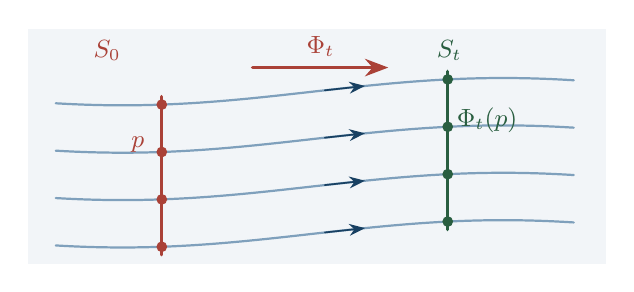
\begin{tikzpicture}[>=Stealth,scale=1.02,line cap=round]
\fill[manifoldblue!6] (-3.55,-1.42) rectangle (3.65,1.5);
\foreach \c in {-1.05,-.46,.13,.72}{
 \draw[manifoldblue!58,thick]
 plot[domain=-3.2:3.25,samples=55]
 ({\x},{\c+.17*sin(38*\x)});
 \draw[->,manifoldblue!70!black,semithick]
 ({.15},{\c+.17*sin(38*.15)})
 --({.65},{\c+.17*sin(38*.65)});
}
\draw[manifoldred,very thick] (-1.88,{-1.15+.17*sin(38*-1.88)})--(-1.88,{.82+.17*sin(38*-1.88)});
\draw[manifoldgreen!75!black,very thick] (1.68,{-1.15+.17*sin(38*1.68)})--(1.68,{.82+.17*sin(38*1.68)});
\foreach \c in {-1.05,-.46,.13,.72}{
 \fill[manifoldred] (-1.88,{\c+.17*sin(38*-1.88)}) circle (1.9pt);
 \fill[manifoldgreen!75!black] (1.68,{\c+.17*sin(38*1.68)}) circle (1.9pt);
}
\node[font=\small,manifoldred] at (-2.56,1.23) {$S_0$};
\node[font=\small,manifoldgreen!75!black] at (1.7,1.23) {$S_t$};
\node[font=\small,manifoldred] at (-2.18,.06) {$p$};
\node[font=\small,manifoldgreen!75!black] at (2.17,.36) {$\Phi_t(p)$};
\draw[->,very thick,manifoldred] (-.75,1.02)--(.94,1.02)
 node[midway,above,font=\small] {$\Phi_t$};
\end{tikzpicture}
\caption{Przepływ przesuwa punkty wzdłuż krzywych całkowych.
Czerwony przekrój poprzeczny $S_0$ przechodzi w zielony $S_t$;
oba przekroje mają dokładnie te same wartości stałej
$y-A\sin(\kappa x)$, gdzie $A=0.17$ i $\kappa=38\pi/180$.
Są to trajektorie pola $X=(1,A\kappa\cos(\kappa x))$.
Jego przepływ to
$\Phi_s(x,y)=(x+s,y+A[\sin(\kappa(x+s))-\sin(\kappa x)])$;
na rysunku $t=1.68-(-1.88)=3.56$.}
\label{fig:rura-przeplywu}
\end{figure}

\begin{przyklad}[Trzy zupełne przepływy]
Na $\R^n$ pole stałe $X=v$ ma $\Phi_t(x)=x+tv$.
Pole Eulera $E=\sum_i x^i\partial_i$ ma $\Phi_t(x)=e^t x$.
Pole obrotowe z~\eqref{eq:obrot} ma
$\Phi_t(a,b)=(a\cos t-b\sin t,a\sin t+b\cos t)$.
Wszystkie rozwiązania są określone dla całego $t\in\R$.
\end{przyklad}

\begin{przyklad}[Ucieczka w skończonym czasie]\label{prz:niezupelne}
Dla $X=x^2\partial_x$ na $\R$ krzywa przez $x_0$ spełnia
\[
 \Phi_t(x_0)=\frac{x_0}{1-tx_0},\qquad x_0\ne0.
\]
Jeśli $x_0>0$, jej dziedzina to $(-\infty,1/x_0)$; jeśli $x_0<0$,
to $(1/x_0,\infty)$. Dla $x_0=0$ krzywa jest stała i istnieje
dla wszystkich czasów. Pole jest gładkie na całej prostej,
ale nie jest zupełne: nieograniczony wzrost rozwiązania powoduje
ucieczkę do nieskończoności w skończonym czasie.
\end{przyklad}

\begin{twierdzenie}[Kryterium przedłużenia i dwa warunki zupełności]
\label{thm:zupelnosc}
Jeśli maksymalna krzywa całkowa ma skończony prawy koniec $b$, to
opuszcza w pobliżu $b$ każdy zwarty podzbiór $M$.
W konsekwencji każde pole na rozmaitości zwartej jest zupełne.
Każde pole o zwartym nośniku na dowolnej rozmaitości także jest zupełne.
\end{twierdzenie}
\begin{proof}
\emph{Kryterium przedłużenia.}
Niech $I_p=(a,b)$ i $b<\infty$. Załóżmy przeciwnie,
że istnieją zbiór zwarty $K\subset M$ i ciąg
$t_j\nearrow b$ taki, że $\gamma_p(t_j)\in K$.
Po wybraniu podciągu mamy $\gamma_p(t_j)\to q\in K$.
Lokalne twierdzenie o istnieniu w $q$ daje otoczenie
$W\ni q$ i $\varepsilon>0$ takie, że z każdego punktu
$W$ można prowadzić rozwiązanie przez wszystkie czasy
$u\in(-\varepsilon,\varepsilon)$.
Dla dużego $j$ zachodzi $\gamma_p(t_j)\in W$
oraz $b-t_j<\varepsilon/2$.
Krzywa
\[
 u\longmapsto\Phi_u(\gamma_p(t_j)),\qquad
 -\varepsilon<u<\varepsilon,
\]
pokrywa się z $u\mapsto\gamma_p(t_j+u)$ w ich wspólnej
dziedzinie, bo obie zaczynają w $\gamma_p(t_j)$.
Możemy więc skleić je w krzywą określoną także dla
$t> b$, sprzecznie z maksymalnością $I_p$.
Przy skończonym lewym końcu stosujemy ten sam argument
do pola $-X$ i czasu odwróconego.

\emph{Zupełność na zbiorach zwartych.}
Jeśli $M$ jest zwarta, każda trajektoria przez cały czas
leży w jednym zwartym zbiorze $M$. Kryterium wyklucza
oba skończone końce $I_p$, zatem $I_p=\R$.
Teraz niech $K=\supp X$ będzie zwarty.
Jeśli $p\notin K$, to $X_p=0$, więc krzywa
stała w $p$ jest, z jednoznaczności, całą krzywą
maksymalną. Jeśli $p\in K$, krzywa nie może wejść
do $M\setminus K$: od chwili wejścia byłaby stała,
a jednoznaczność, zastosowana także wstecz w czasie,
zmusiłaby ją do bycia stałą już w chwili zero.
W obu przypadkach obraz $\gamma_p$ leży w zwartym
zbiorze $K\cup\{p\}$; kryterium znów daje $I_p=\R$.
\end{proof}

\begin{uwaga}[Nie mylić zupełności z brakiem zer]
Zupełne pole może mieć zera (obrót na płaszczyźnie), a pole bez zer
może być niezupełne, np.\ $X=(1+x^2)\partial_x$ na $\R$.
Dla rozmaitości z brzegiem pole musi dodatkowo być styczne do brzegu,
aby dać dwustronny przepływ zachowujący tę rozmaitość.
Istotnie, dyfeomorfizmy zachowują brzeg, więc różniczkowanie
krzywej $t\mapsto\Phi_t(p)$ dla $p\in\partial M$ daje
$X_p\in T_p\partial M$. Odwrotnie, dla pola stycznego do brzegu
rozwiązujemy równanie również na $\partial M$; jednoznaczność
w lokalnym przedłużeniu pola zapewnia, że jego krzywe przez
brzeg pozostają na brzegu. Krzywe z wnętrza nie mogą go
przekroczyć, bo przy pierwszym spotkaniu jednoznaczność wstecz
wymuszałaby wcześniejszy pobyt na brzegu.
Pole skierowane do wnętrza na brzegu daje zwykle przepływ tylko
dla małych dodatnich czasów, co wykorzystamy do budowania kołnierza.
\end{uwaga}

\section{Geometria przepływu: prostowanie, niezmienniki, komutowanie}
\label{sec:prostowanie}

\begin{definicja}[Orbita i nasycenie przez przepływ]
\index{orbita i nasycenie przez przeplyw@Orbita i nasycenie przez przepływ}
\emph{Orbitą} punktu $p$ pod przepływem pola $X$ jest
$\mathcal O_X(p)=\{\Phi_t(p):t\in I_p\}$.
Dla $A\subseteq M$ jego \emph{nasycenie przez przepływ}
to suma orbit punktów z $A$:
\[
 \operatorname{Sat}_X(A)=\bigcup_{p\in A}\mathcal O_X(p).
\]
Zbiór $A$ jest \emph{nasycony przez $X$}, gdy
$\operatorname{Sat}_X(A)=A$, czyli gdy
$p\in A$ i $t\in I_p$ pociągają za sobą
$\Phi_t(p)\in A$.
\end{definicja}

To jest nasycenie względem relacji ,,leżeć na tej samej
orbicie'' w sensie Definicji~\ref{def:nasycenie}.
Istotnie, gdy $q=\Phi_s(p)$, to
$I_q=I_p-s$ i $\mathcal O_X(q)=\mathcal O_X(p)$
na mocy Twierdzenia~\ref{thm:przeplyw}; orbity rozcinają
więc $M$ na rozłączne klasy. Na przykład dla
$X=\partial_x$ na $\R^2$ nasyceniem
$\{0\}\times(0,1)$ jest cały pas $\R\times(0,1)$.

\begin{twierdzenie}[Twierdzenie o prostowaniu pola]\label{thm:flowbox}
Jeśli $X_p\ne0$, to istnieją współrzędne $(t,z^2,\ldots,z^n)$
w otoczeniu $p$, w których $X=\partial_t$. W tych współrzędnych
lokalny przepływ ma postać
\[
 (t,z^2,\ldots,z^n)\longmapsto(t+s,z^2,\ldots,z^n).
\]
\end{twierdzenie}
\begin{proof}
Wybieramy małą $(n-1)$-wymiarową podrozmaitość $S$
przechodzącą przez $p$ i poprzeczną do $X_p$, oraz parametryzację
$\sigma\colon V\subset\R^{n-1}\to S$ z $\sigma(0)=p$.
Można ją zbudować bez dodatkowego twierdzenia: wybieramy mapę
z $p=0$ i po liniowej zmianie współrzędnych z pierwszą składową
$X_p$ niezerową; bierzemy $S=\{x^1=0\}$ w tej mapie.
Odwzorowanie $F(t,z)=\Phi_t(\sigma(z))$ ma w $(0,0)$
różniczkę, której pierwszą kolumną jest $X_p$, a pozostałe kolumny
rozpinają $T_pS$. Jest więc izomorfizmem. Z twierdzenia o funkcji
odwrotnej $F$ jest lokalnym dyfeomorfizmem. Zmniejszamy jego
dziedzinę do produktu $(-\varepsilon,\varepsilon)\times V_0$.
Ponieważ $\partial_tF(t,z)=X_{F(t,z)}$, we współrzędnych $F^{-1}$
pole ma postać $\partial_t$. Prawo grupowe daje
$\Phi_s(F(t,z))=F(t+s,z)$, dopóki $t$ i $t+s$ leżą
w tym przedziale. To wyjaśnia lokalny zakres wzoru z tezy.
\end{proof}

\begin{uwaga}
Pola nie można wyprostować w zerze $X_p=0$: dyfeomorfizm przenosi
wektor zerowy na wektor zerowy, natomiast $\partial_t$ nigdzie
nie znika. W zerze lokalne trajektorie i zachowanie przepływu
bada się innymi metodami niż prostowanie pola.
\end{uwaga}

\begin{stwierdzenie}[Lokalne twierdzenie Frobeniusa]
\label{prop:frobenius-lokalny}
Gładki rozkład inwolutywny $\mathcal D$ stałego rzędu $k$
ma lokalnie współrzędne, w których jest rozpięty przez pierwsze
$k$ pól współrzędnych.
\end{stwierdzenie}
\begin{proof}
Przeprowadzimy indukcję po $k$, jednocześnie dla wszystkich
wymiarów rozmaitości. Dla $k=0$ teza jest natychmiastowa.
Dla $k\ge1$ wybieramy lokalną bazę $X_1,\ldots,X_k$ rozkładu
i prostujemy niezerowe $X_1$. Mamy więc współrzędne $(t,z)$
w produkcie wokół $(0,0)$, z $X_1=\partial_t$.
Od każdego $X_j$, $j\ge2$, odejmujemy jego składową w kierunku
$\partial_t$. Otrzymane pola $Y_2,\ldots,Y_k$ nie mają tej
składowej, a wraz z $\partial_t$ nadal stanowią bazę $\mathcal D$.
Jeśli $k=1$, dowód jest już zakończony.

Niech $B(t,z)$ będzie macierzą o $k-1$ kolumnach złożonych
ze składowych $Y_2,\ldots,Y_k$ w kierunkach $z$.
Inwolutywność daje $[\partial_t,Y_j]\in\mathcal D$;
ponieważ ten nawias nie ma składowej czasowej, jest kombinacją
samych $Y_2,\ldots,Y_k$. Zatem
\[
 \partial_tB(t,z)=B(t,z)A(t,z)
\]
dla pewnej gładkiej macierzy kwadratowej $A$.
Gładkość współczynników wynika z rozwiązania układu za pomocą
niezerowego minora macierzy $B$, po zmniejszeniu otoczenia.
Rozwiązujemy macierzowe równanie
\[
 \partial_tQ(t,z)=-A(t,z)Q(t,z),\qquad Q(0,z)=I.
\]
Istnienie i gładka zależność od $z$ wynikają z
Twierdzenia~\ref{thm:ode}: dołączamy zmienne z równaniami
$t'=1$, $z'=0$. Po zmniejszeniu produktu $Q$ jest odwracalna,
bo $Q(0,0)=I$. Reguła iloczynu daje
\[
 \partial_t(BQ)=BAQ-BAQ=0,\qquad B(t,z)Q(t,z)=B(0,z).
\]
Kolumny $BQ$ wyznaczają więc nową bazę pól pionowych
niezależnych od $t$, rozpinającą te same kierunki co kolumny $B$.
Na przekroju $t=0$ tworzą rozkład rzędu $k-1$.
Jest on inwolutywny: nawiasy tych pól nie mają składowej
czasowej, należą do $\mathcal D$ i nie zależą od $t$;
reguła Leibniza dla nawiasu rozszerza to na dowolne sekcje.
Z założenia indukcyjnego istnieje zmiana współrzędnych $z$
prostująca ten rozkład. Stosujemy ją niezależnie od $t$.
Ponieważ baza pionowa nie zależy od czasu, w całym produkcie
$\mathcal D$ jest rozpięty przez $\partial_t$ i pierwsze
$k-1$ nowych pól współrzędnych na przekroju. To kończy indukcję.
\end{proof}

\begin{stwierdzenie}[Funkcje i pola niezmiennicze]\label{prop:inwarianty}
Dla zupełnego $X$ funkcja $f$ jest stała na każdej jego trajektorii
wtedy i tylko wtedy, gdy $X(f)=0$. Przepływ zawsze zachowuje
pole, które go generuje: $(\Phi_t)_*X=X$.
Dla innego pola $Y$ następujące warunki są równoważne:
\begin{enumerate}[label=(\roman*)]
\item $[X,Y]=0$;
\item $(\Phi_t)_*Y=Y$ dla wszystkich $t$;
\item lokalne przepływy $X$ i $Y$ komutują tam, gdzie są określone.
\end{enumerate}
W przypadku pól zupełnych ostatni punkt oznacza
$\Phi_t^X\circ\Phi_s^Y=\Phi_s^Y\circ\Phi_t^X$ dla wszystkich $s,t$.
\end{stwierdzenie}
\begin{proof}
Reguła łańcucha daje
$\frac{\dd}{\dd t}f(\Phi_t(p))=X(f)(\Phi_t(p))$.
Druga równość wynika z~\eqref{eq:przeplyw-generuje}.
Dla $Y$ użyjemy wzoru udowodnionego poniżej w
Stwierdzeniu~\ref{prop:lie-ewolucja}:
$\frac{\dd}{\dd t}\Phi_t^*Y=\Phi_t^*[X,Y]$.
Jeśli (i) zachodzi, cofnięte pole ma zerową pochodną
i wartość $Y$ w chwili zero, więc $\Phi_t^*Y=Y$.
Ponieważ $\Phi_t^*Y=(\Phi_{-t})_*Y$, jest to (ii).
Odwrotnie, różniczkowanie (ii) w zerze daje $[X,Y]=0$.
Niech $\Psi_s$ oznacza maksymalny przepływ $Y$. Przy (ii)
dla każdego ustalonego $t$ krzywa $s\mapsto\Phi_t(\Psi_s(p))$
ma pochodną $\dd\Phi_t(Y)=Y$ i zaczyna w $\Phi_t(p)$.
Jednoznaczność daje $\Phi_t(\Psi_s(p))=\Psi_s(\Phi_t(p))$.
Ponieważ $\Phi_t$ jest globalnym dyfeomorfizmem, zastosowanie
tego samego argumentu do $\Phi_{-t}$ pokazuje równość
maksymalnych przedziałów $Y$ przez $p$ i $\Phi_t(p)$.
Wyjaśnia to również zgodność dziedzin w (iii).
Różniczkując (iii) po $s$ w zerze, odzyskujemy
$\dd\Phi_t(Y_p)=Y_{\Phi_t(p)}$, czyli (ii).
\end{proof}

\begin{przyklad}[Pierwsza całka]
Dla pola obrotowego $R=-y\partial_x+x\partial_y$
funkcja $f(x,y)=x^2+y^2$ spełnia $R(f)=0$.
Jej dodatnie poziomice są okręgami, po których biegnie przepływ;
poziomica zerowa to nieruchomy punkt $(0,0)$, a ujemne są puste.
W zagadnieniach dynamiki taka funkcja to \emph{pierwsza całka}.
\end{przyklad}

\section{Pochodna Liego: porównywanie danych w różnych punktach}
\label{sec:liego}

Nie można po prostu odjąć wektorów $Y_{\Phi_t(p)}$ i $Y_p$:
należą do różnych przestrzeni stycznych. Przepływ $X$ dostarcza
\emph{kanonicznego w tej sytuacji} sposobu ich porównania:
różniczka odwrotnego przepływu przenosi pierwszy z nich do $T_pM$.
Otrzymujemy odpowiedź na pytanie, jak obiekt zmienia się
wraz z ruchem generowanym przez $X$.

\begin{definicja}\label{def:pochodna-liego}
Dla funkcji $f$ i pola $Y$ określamy
\begin{align}
 (\Lie_Xf)(p)
 &=\left.\frac{\dd}{\dd t}\right|_{0}f(\Phi_t(p))=X(f)(p),
 \label{eq:lie-f}\\
 (\Lie_XY)_p
 &=\left.\frac{\dd}{\dd t}\right|_{0}
 (\dd\Phi_{-t})_{\Phi_t(p)}Y_{\Phi_t(p)}.
 \label{eq:lie-y}
\end{align}
Definicja jest lokalna: przepływ jest potrzebny tylko dla małego $t$.
Wzór~\eqref{eq:lie-y} zapisujemy krótko jako
$\Lie_XY=\left.\frac{\dd}{\dd t}\right|_0\Phi_t^*Y$.
\end{definicja}


\begin{figure}[!htbp]
\centering
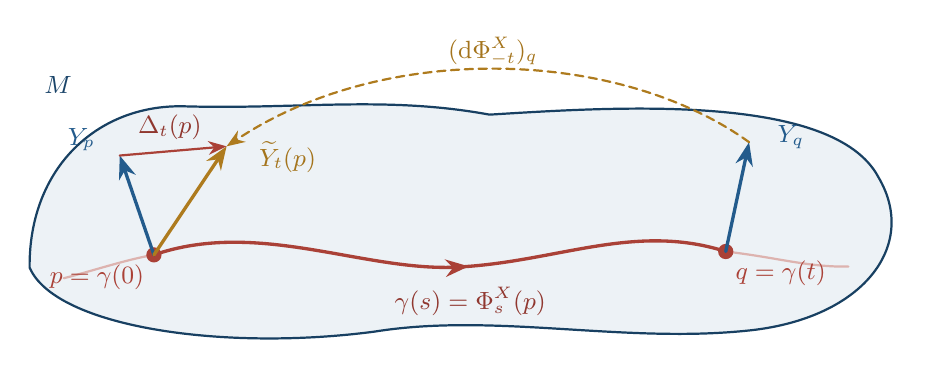
\begin{tikzpicture}[>=Stealth,scale=1.06,line cap=round,line join=round]
% Jedno spójne otoczenie na M; p i q są punktami czerwonej trajektorii.
\filldraw[fill=manifoldblue!8,draw=manifoldblue!70!black,thick]
 (-5.14,-.67) .. controls (-5.15,.52) and (-4.33,1.28) .. (-3.3,1.26)
 .. controls (-1.92,1.22) and (-.88,1.39) .. (.37,1.16)
 .. controls (1.84,1.25) and (4.49,1.43) .. (5.03,.41)
 .. controls (5.52,-.42) and (4.83,-1.3) .. (3.44,-1.43)
 .. controls (1.94,-1.58) and (.42,-1.21) .. (-1.01,-1.44)
 .. controls (-2.84,-1.68) and (-4.84,-1.38) .. cycle;
\node[font=\small,manifoldblue!75!black] at (-4.8,1.51) {$M$};
\coordinate (P) at (-3.65,-.52);
\coordinate (Q) at (3.2,-.48);
% Ciągła krzywa całkowa; wyraźne punkty p, q i kierunek czasu.
\draw[manifoldred!40,thick] (-4.73,-.8)
 .. controls (-4.38,-.71) and (-3.96,-.57) .. (P);
\draw[manifoldred,very thick,postaction={decorate},
 decoration={markings,mark=at position .55 with {\arrow{Stealth}}}]
 (P) .. controls (-2.43,-.1) and (-1.21,-.69) .. (-.1,-.67)
 .. controls (1.13,-.63) and (2.08,-.12) .. (Q);
\draw[manifoldred!40,thick] (Q)
 .. controls (3.81,-.55) and (4.19,-.67) .. (4.67,-.66);
\node[font=\small,manifoldred!85!black] at (.14,-1.08)
 {$\gamma(s)=\Phi_s^X(p)$};
\fill[manifoldred] (P) circle (2.6pt)
 node[below left,font=\small] {$p=\gamma(0)$};
\fill[manifoldred] (Q) circle (2.6pt)
 node[below right,font=\small] {$q=\gamma(t)$};
% Wektory porównywane po sprowadzeniu do T_p M.
\draw[->,manifoldblue,very thick] (P)--(-4.06,.67);
\draw[->,manifoldgold!85!black,very thick] (P)--(-2.78,.78);
\node[font=\small,manifoldblue] at (-4.52,.86) {$Y_p$};
\node[font=\small,manifoldgold!80!black] at (-2.05,.65)
 {$\widetilde Y_t(p)$};
\draw[->,manifoldred,thick] (-4.06,.67)--(-2.78,.78);
\node[font=\small,manifoldred!85!black] at (-3.46,1.01) {$\Delta_t(p)$};
% Wektor Y_q oraz schemat cofnięcia jego wartości, odrębny od trajektorii.
\draw[->,manifoldblue,very thick] (Q)--(3.48,.83);
\node[font=\small,manifoldblue] at (3.98,.89) {$Y_q$};
\draw[->,manifoldgold!85!black,thick,densely dashed]
 (3.48,.83) .. controls (1.93,1.95) and (-.88,2.05) .. (-2.78,.78);
\node[font=\small,manifoldgold!80!black] at (.41,1.92)
 {$(\dd\Phi_{-t}^X)_q$};
\end{tikzpicture}
\caption{Punkty $p=\gamma(0)$ i $q=\gamma(t)=\Phi_t^X(p)$ leżą
na tej samej krzywej całkowej na $M$; czerwona strzałka pokazuje
ruch w czasie od $p$ do $q$. Wektor $Y_q$ cofamy różniczką
przepływu do $T_pM$, otrzymując $\widetilde Y_t(p)$.
Tam porównujemy go z $Y_p$; $\Delta_t(p)$ jest ich różnicą.
Przerywana strzałka przedstawia transport wektora, nie ruch punktu.}
\label{fig:pochodna-liego}
\end{figure}

Dokładnie, oznaczając $q=\Phi_t^X(p)$, mamy
\[
 \widetilde Y_t(p):=(\dd\Phi_{-t}^X)_qY_q\in T_pM,\qquad
 (\Lie_XY)_p=\lim_{t\to0}\frac{\widetilde Y_t(p)-Y_p}{t}.
\]
Dla każdego małego $t$ oba odejmowane wektory leżą w $T_pM$.
Rysunek~\ref{fig:pochodna-liego} pokazuje różnicę $\Delta_t(p)$,
której iloraz przez $t$ ma granicę dla $t\to0$.


\begin{twierdzenie}\label{thm:lie-nawias}
Dla dowolnych pól $X,Y$ zachodzi
\begin{equation}\label{eq:lie-nawias}
 \Lie_XY=[X,Y].
\end{equation}
Zatem pochodna Liego funkcji jest działaniem derywacji,
a pochodna Liego pola jest nawiasem.
\end{twierdzenie}
\begin{proof}
Ustalmy $p\in M$ i $f\in C^\infty(M)$. Pracujemy w otoczeniu $p$
i dla na tyle małych $|t|$, aby lokalny przepływ $\Phi_t=\Phi_t^X$
oraz $\Phi_{-t}$ były określone we wszystkich rozważanych punktach.
Z definicji cofnięcia pola, przy $q=\Phi_t(p)$,
\[
 Z_t(p):=(\Phi_t^*Y)_p=(\dd\Phi_{-t})_qY_q\in T_pM.
\]
Wektory $Z_t(p)$ leżą więc w \emph{jednej} przestrzeni $T_pM$,
a $Z_0(p)=Y_p$. Aby obliczyć ich pochodną, zadziałajmy nimi
na dowolną funkcję $f$. Definicja różniczki daje
\begin{equation}\label{eq:lie-pullback-funkcja}
 Z_t(p)(f)
 =Y_q(f\circ\Phi_{-t})
 =Y(f\circ\Phi_{-t})(\Phi_t(p)).
\end{equation}
Oznaczmy $F(t,r):=f(\Phi_{-t}(r))$ dla $r$ w otoczeniu $p$.
Ponieważ $\frac{\dd}{\dd t}\Phi_{-t}(r)=-X_{\Phi_{-t}(r)}$,
reguła łańcucha daje
\[
 F(0,r)=f(r),\qquad
 \left.\frac{\partial F}{\partial t}\right|_{(0,r)}
 =-X(f)(r).
\]
Niech $H(t,r):=Y_r(F(t,\cdot))$. Wtedy prawa strona
\eqref{eq:lie-pullback-funkcja} jest równa $H(t,\Phi_t(p))$.
Różniczkując to złożenie, musimy uwzględnić zarówno zmianę
funkcji $H$ z czasem, jak i ruch punktu $\Phi_t(p)$:
\begin{align*}
 \left.\frac{\dd}{\dd t}H(t,\Phi_t(p))\right|_{t=0}
 &=\left.\frac{\partial H}{\partial t}\right|_{(0,p)}
   +X_p\bigl(H(0,\cdot)\bigr) \\
 &=-Y_p\bigl(X(f)\bigr)+X_p\bigl(Y(f)\bigr).
\end{align*}
W drugim kroku użyliśmy $H(0,\cdot)=Y(f)$ oraz
$\partial_tH(0,p)=Y_p\bigl(\partial_tF(0,\cdot)\bigr)$.
Zamiana kolejności $Y$ i $\partial_t$ jest dopuszczalna:
w lokalnych współrzędnych $Y=\sum_iY^i(r)\partial_{r^i}$,
współczynniki $Y^i$ nie zależą od $t$, a funkcja $F$ jest gładka.
Wreszcie, ponieważ $Z_t(p)$ jest gładką krzywą w $T_pM$,
jej pochodną można obliczyć po przyłożeniu do $f$. Otrzymujemy
\[
 (\Lie_XY)_p(f)
 =\left.\frac{\dd}{\dd t}Z_t(p)(f)\right|_{t=0}
 =X(Yf)(p)-Y(Xf)(p)=[X,Y]_p(f).
\]
Równość zachodzi dla każdej funkcji gładkiej $f$. Funkcje gładkie
rozróżniają wektory styczne: wystarczy wziąć funkcje, które
w pobliżu $p$ pokrywają się ze współrzędnymi lokalnymi.
Zatem $(\Lie_XY)_p=[X,Y]_p$; punkt $p$ był dowolny.
\end{proof}

\begin{stwierdzenie}\label{prop:lie-ewolucja}
Na wspólnych dziedzinach lokalnego przepływu pola $X$ zachodzi
\[
 \frac{\dd}{\dd t}\Phi_t^*Y=\Phi_t^*[X,Y].
\]
\end{stwierdzenie}
\begin{proof}
Dla dyfeomorfizmu $F$ cofnięcie pola oznacza $F^*Y=(F^{-1})_*Y$.
Reguła łańcucha daje $(F\circ G)^*=G^*F^*$.
Prawo grupowe przepływu pozwala zatem napisać
$\Phi_{t+h}^*Y=\Phi_t^*(\Phi_h^*Y)$.
Ustalamy punkt i dostatecznie małe wspólne otoczenie, aby
wszystkie te odwzorowania były określone dla $h$ bliskiego zeru.
Różniczkujemy po $h$ w zerze: liniowa mapa cofająca przez
ustalone $\Phi_t$ nie zależy od $h$, a
$\left.\partial_h\right|_0\Phi_h^*Y=[X,Y]$
na mocy Twierdzenia~\ref{thm:lie-nawias}.
\end{proof}

\begin{uwaga}[Ten sam rachunek we współrzędnych]
W lokalnych współrzędnych, zapisując pola jako kolumny funkcji,
gładkość przepływu daje przy $t\to0$
\[
 \Phi_t(x)=x+tX(x)+o(t),\qquad
 \dd\Phi_t|_x=I+t\,\dd X|_x+o(t),
\]
a stąd $\dd\Phi_{-t}|_{\Phi_t(x)}=(\dd\Phi_t|_x)^{-1}
=I-t\,\dd X|_x+o(t)$ oraz
$Y(\Phi_t(x))=Y(x)+t\,\dd Y|_xX(x)+o(t)$.
Po pomnożeniu obu wyrażeń otrzymujemy
\[
 (\Phi_t^*Y)(x)=Y(x)+t\bigl(\dd Y|_xX(x)-\dd X|_xY(x)\bigr)+o(t).
\]
Zatem składowa $j$ pochodnej wynosi
$\sum_i(X^i\partial_iY^j-Y^i\partial_iX^j)$,
co zgadza się ze wzorem na nawias Liego.
\end{uwaga}

\begin{przyklad}[Obliczenie w polu przesunięć]
Dla $X=\partial_x$ i $Y=x\partial_y$ mamy
$\Phi_t(x,y)=(x+t,y)$. W punkcie $q=(x+t,y)$ jest
$Y_q=(x+t)\partial_y$, a cofająca różniczka przesunięcia
działa identycznościowo na wektory. Zatem
\[
 ((\Phi_t)^*Y)_{(x,y)}=(x+t)\partial_y,
 \qquad \Lie_XY=\partial_y.
\]
Nie chodzi o różnicę położeń punktów, tylko o zmianę pola
po przeniesieniu obu wektorów do tej samej przestrzeni stycznej.
\end{przyklad}

\begin{figure}[!htbp]
\centering
\begin{tikzpicture}[>=Stealth,scale=1.12,line cap=round,line join=round]
% Cztery kroki komutatora dla X=\partial_x, Y=(1+x)\partial_y.
\coordinate (P) at (-2,-.68);
\coordinate (A) at (.7,-.68);
\coordinate (B) at (.7,1.04);
\coordinate (C) at (-2,1.04);
\coordinate (Q) at (-2,.04);
\fill[manifoldblue!5] (-2.65,-1.15) rectangle (1.38,1.52);
\draw[manifoldblue!22,thin] (-2.65,-1.15) rectangle (1.38,1.52);
\draw[->,very thick,manifoldblue] (P)--(A)
 node[midway,below,font=\small] {$\Phi_t^X$};
\draw[->,very thick,manifoldgreen] (A)--(B)
 node[midway,right,font=\small] {$\Phi_t^Y$};
\draw[->,very thick,manifoldblue] (B)--(C)
 node[midway,above,font=\small] {$\Phi_{-t}^X$};
\draw[->,very thick,manifoldgreen] (C)--(Q)
 node[midway,left,font=\small] {$\Phi_{-t}^Y$};
\fill[manifoldred] (P) circle (2.5pt) node[below left,font=\small] {$p$};
\fill[manifoldred] (Q) circle (2.5pt) node[left,font=\small] {$C_t(p)$};
\draw[->,thick,manifoldred,densely dashed] (-1.66,-.68)--(-1.66,.04)
 node[midway,right,font=\small] {$t^2[X,Y]_p$};
\node[font=\footnotesize,align=center] at (3.7,.52)
 {$C_t=\Phi_{-t}^Y\circ\Phi_{-t}^X$\\[2pt]
 $\circ\Phi_t^Y\circ\Phi_t^X$};
\node[font=\footnotesize,align=center,text width=3.4cm] at (3.75,-.6)
 {Końcowy punkt leży o rząd $t^2$ ponad początkiem.};
\end{tikzpicture}
\caption{Komutator małych przepływów. Po przejściu kolejno wzdłuż
$X,Y,-X,-Y$ droga zwykle się nie zamyka; wyraz przemieszczenia rzędu $t^2$ jest wyznaczony przez nawias
$[X,Y]$. Jeśli nawias znika, pierwszy niezerowy wyraz może mieć
wyższy rząd. Rysunek schematycznie ilustruje przykład
$X=\partial_x$, $Y=(1+x)\partial_y$.}
\label{fig:komutator-przeplywow}
\end{figure}

Jeśli $C_t=\Phi_{-t}^Y\circ\Phi_{-t}^X\circ\Phi_t^Y\circ\Phi_t^X$, to
w dowolnej mapie wokół $p$ (i dla małego $t$)
\[
 x(C_t(p))=x(p)+t^2\,\dd x_p([X,Y]_p)+O(t^3).
\]
W przykładzie $X=\partial_x$, $Y=(1+x)\partial_y$ i $p=(0,0)$
można to policzyć dokładnie: $p\to(t,0)\to(t,t+t^2)
\to(0,t+t^2)\to(0,t^2)$. Geometria rysunku zgadza się więc ze
znakiem konwencji~\eqref{eq:nawias-def}.

Uzasadnijmy także wzór ogólny, zamiast wnioskować z jednego przykładu.
W ustalonej mapie przepływ gładkiego pola $Z$ ma rozwinięcie
\[
 \Phi_t^Z(x)=x+tZ(x)+\tfrac12t^2 DZ(x)Z(x)+O(t^3),
\]
bo druga pochodna krzywej całkowej w zerze to $DZ(x)Z(x)$.
Oznaczmy kolejne punkty czterech kroków przez $x_1,\ldots,x_4$.
Rozwijając pola w punktach pośrednich, dostajemy
\begin{align*}
 x_1&=x+tX+\tfrac12t^2 DX\,X+O(t^3),\\
 x_2&=x+t(X+Y)+t^2(\tfrac12 DX\,X+DY\,X+\tfrac12 DY\,Y)+O(t^3),\\
 x_3&=x+tY+t^2(DY\,X+\tfrac12 DY\,Y-DX\,Y)+O(t^3),\\
 x_4&=x+t^2(DY\,X-DX\,Y)+O(t^3).
\end{align*}
Wszystkie pola i ich macierze pochodnych po prawej stronie
są obliczone w $x$. Równość $DY\,X-DX\,Y=[X,Y](x)$
wynika ze wzoru~\eqref{eq:nawias-wspolrzedne}.
Reszty $O(t^3)$ są rozumiane w tej mapie, dla punktów w
dostatecznie małym otoczeniu i małego czasu, gdy złożenia istnieją.


\begin{uwaga}[Znaczenie znaku]
W~\eqref{eq:lie-y} wektor cofamy przez $\Phi_{-t}$.
Przy tej konwencji $\Lie_XY=[X,Y]$. Gdyby transportować
$Y_p$ w przód i porównywać z $Y_{\Phi_t(p)}$ w punkcie
$\Phi_t(p)$ w odwrotnej kolejności, otrzymalibyśmy zapis
z przeciwnym znakiem. Przed rachunkiem warto zawsze ustalić,
które dwa wektory są porównywane i w jakim punkcie.
\end{uwaga}

\section{Pola zależne od czasu i izotopie}
\label{sec:izotopie}

Przepływ pola stałego w czasie spełnia lokalne prawo grupowe;
dla pola zupełnego tworzy jednoparametrową grupę dyfeomorfizmów.
W topologii różniczkowej często trzeba deformować obiekty według
zaplanowanego ruchu, którego prędkość może zmieniać się z czasem.

\begin{definicja}
\emph{Pole zależne od czasu} to rodzina $X_t\in\X(M)$,
$t\in[0,1]$, gładka łącznie w $(t,p)$ (na końcach przedziału
w sensie lokalnego gładkiego przedłużenia). Jej krzywe całkowe spełniają nieautonomiczne równanie
$\gamma'(t)=(X_t)_{\gamma(t)}$. Odwzorowanie ewolucji
$F_{t,s}(p)$ przenosi położenie w chwili $s$ do położenia
w chwili $t$, tam gdzie rozwiązanie istnieje.
\end{definicja}

Dodanie czasu jako zmiennej sprowadza to równanie do autonomicznego
pola $\widehat X=\partial_t+X_t$ na czasoprzestrzeni.
Krzywa tego pola startująca w $(s,p)$ ma postać
$(s+u,F_{s+u,s}(p))$. Twierdzenie~\ref{thm:ode}, zastosowane
lokalnie także do przedłużeń przy końcach przedziału, daje
gładkość ewolucji łącznie w $(t,s,p)$. Jednoznaczność daje prawo
\begin{equation}\label{eq:ewolucja}
 F_{s,s}=\id,\qquad F_{u,t}\circ F_{t,s}=F_{u,s},
 \qquad F_{s,t}=F_{t,s}^{-1}.
\end{equation}
Równości obowiązują tam, gdzie odpowiednie rozwiązania istnieją;
$F_{t,s}$ jest dyfeomorfizmem swojej otwartej dziedziny na obraz,
z odwrotnością $F_{s,t}$.
Zwykle $F_{t,0}$ \emph{nie} spełnia
$F_{t+s,0}=F_{t,0}\circ F_{s,0}$, bo samo pole się zmienia.
Jeżeli nośniki wszystkich $X_t$ mieszczą się w jednym zwartym
$K\subset M$, ewolucja istnieje dla całego przedziału $[0,1]$:
poza $K$ krzywe stałe są rozwiązaniami, a jednoznaczność
w obu kierunkach czasu nie pozwala trajektorii z $K$ wyjść
poza $K$. Trajektoria startująca w $p$ pozostaje więc w
$K\cup\{p\}$. Jej podniesienie do czasoprzestrzeni leży
w zwartym $[0,1]\times(K\cup\{p\})$. Argument przedłużania
z dowodu Twierdzenia~\ref{thm:zupelnosc}, z lokalnymi przedłużeniami
pola na końcach przedziału, wyklucza skończony czas zakończenia
rozwiązania przed dojściem do wymaganej chwili. Istotny jest
\emph{wspólny} zwarty nośnik, a nie tylko zwartość każdego z nośników osobno.

\begin{definicja}
Gładka rodzina dyfeomorfizmów $h_t\colon M\to M$ z
$h_0=\id_M$ to \emph{izotopia otoczenia}.
Gładka rodzina osadzeń $i_t\colon N\hookrightarrow M$ to
\emph{izotopia osadzeń}. Drugie pojęcie dotyczy tylko ruchu
podrozmaitości, pierwsze przesuwa całe otoczenie.
Osadzenie oznacza tu zanurzenie w sensie Rozdziału~\ref{ch:rozmaitosci},
czyli immersję będącą homeomorfizmem na obraz.
Nośnikiem izotopii otoczenia nazywamy domknięcie zbioru
$\{p\in M:h_t(p)\ne p\text{ dla pewnego }t\in[0,1]\}$.
\end{definicja}

Każda izotopia otoczenia jest generowana przez pole zależne od
czasu: dla $q=h_t(p)$ kładziemy
\begin{equation}\label{eq:generator-izotopii}
 (X_t)_q=\left.\frac{\partial h_t(p)}{\partial t}
 \right|_{p=h_t^{-1}(q)}.
\end{equation}
Gładkość tego pola wymaga także gładkości $(t,q)\mapsto h_t^{-1}(q)$.
Wynika ona z twierdzenia o funkcji odwrotnej zastosowanego do
$H(t,p)=(t,h_t(p))$: różniczka jest blokowo trójkątna z
odwracalnymi blokami $1$ i $\dd h_t$. Przy $t=0,1$ stosujemy
lokalne przedłużenia; pierwsza współrzędna pozostaje czasem.
Jednoznaczność rozwiązań daje $h_t=F_{t,0}$.
W szczególności pole zależne od czasu
o wspólnym zwartym nośniku buduje izotopię otoczenia
stałą poza tym nośnikiem.

\begin{twierdzenie}[Rozszerzenie izotopii, wersja zwarta]
\label{thm:rozszerzenie-izotopii}
Niech $M$ będzie rozmaitością bez brzegu,
$N$ jej zwartą podrozmaitością bez brzegu,
a $i_t\colon N\hookrightarrow M$, $t\in[0,1]$, gładką
izotopią osadzeń. Istnieje izotopia otoczenia $h_t$ taka, że
$h_t\circ i_0=i_t$. Jej nośnik można umieścić w dowolnym
otwartym otoczeniu zwartego śladu
$\bigcup_{t\in[0,1]}i_t(N)$.
\end{twierdzenie}
\begin{proof}
\emph{Krok 1: pole na śladzie izotopii.}
Zbudujmy \emph{ślad w czasoprzestrzeni}
\[
 \mathcal T:=\{(t,i_t(x)):t\in[0,1],\ x\in N\}
 \subset[0,1]\times M.
\]
Odwzorowanie $I(t,x)=(t,i_t(x))$ jest różnowartościowe:
z równości pierwszych współrzędnych mamy ten sam $t$,
a różnowartościowość $i_t$ daje ten sam $x$.
Jego różniczka jest injektywna: jeśli
$\dd I_{(t,x)}(a,v)=0$, to pierwsza współrzędna daje
$a=0$, a następnie $\dd (i_t)_x(v)=0$ wymusza $v=0$.
Ponieważ $[0,1]\times N$ jest zwarta, $I$ jest osadzeniem
(ciągła bijekcja z przestrzeni zwartej na podprzestrzeń
Hausdorffa ma ciągłą odwrotność). Zatem $\mathcal T$
jest zwartą podrozmaitością z brzegiem w $[0,1]\times M$.
Wyjaśnijmy postać lokalną także dla $t=0,1$. W lokalnych
współrzędnych $u$ na $N$ wybieramy $k=\dim N$ składowych $i_t(u)$,
których różniczka względem $u$ jest odwracalna. Odwzorowanie
$(t,u)\mapsto(t,i_t^1(u),\ldots,i_t^k(u))$ jest lokalnym
dyfeomorfizmem. Pozostałe składowe śladu są więc wykresem
$w=b(t,z)$. Zmiana $(t,z,w)\mapsto(t,z,w-b(t,z))$ prostuje
ślad i zachowuje czas, a zatem również brzeg przy $t=0,1$.
Homeomorficzność $I$ na obraz pozwala zmniejszyć otoczenie tak,
aby nie zawierało innych fragmentów śladu.
Wzdłuż niej mamy dobrze określony \emph{pionowy} wektor
\[
 V(t,i_t(x)):=\frac{\partial i_t(x)}{\partial t}
 \in T_{i_t(x)}M.
\]
Jest gładki, bo $I$ ma gładką odwrotność na $\mathcal T$.

\emph{Krok 2: przedłużenie o małym nośniku.}
Niech $O\subset M$ będzie wskazanym otwartym otoczeniem
rzutu $\mathcal T$ na $M$. Wokół każdego punktu
$\mathcal T$ wybieramy lokalne współrzędne na
$[0,1]\times M$, w których $\mathcal T$ ma postać
normalną opisaną powyżej; otoczenia wybieramy wewnątrz
$[0,1]\times O$. W lokalnej trywializacji $TM$
składowe wektora $V$ są gładkimi funkcjami współrzędnych
na $\mathcal T$; przedłużamy je, nadając im te same
wartości w pobliskich kierunkach normalnych.
Otrzymujemy lokalne pola pionowe $V^{(j)}$, których
ograniczenia do $\mathcal T$ są równe $V$.
Zwartość $\mathcal T$ pozwala wybrać skończenie wiele
takich otoczeń i nieujemne gładkie funkcje odcinające $\chi_j$
o zwartych nośnikach w tych otoczeniach, z
$\sum_j\chi_j>0$ na $\mathcal T$.
Na otwartym zbiorze $U=\{\sum_j\chi_j>0\}$ kładziemy
$Y=(\sum_j\chi_j V^{(j)})/(\sum_k\chi_k)$,
przedłużając każde $\chi_j V^{(j)}$ przez zero poza jego otoczenie.
Na $\mathcal T$ wszystkie składniki $V^{(j)}$ są równe
$V$, więc $Y|_{\mathcal T}=V$.
Wybieramy jeszcze funkcję odcinającą $\rho$ równą $1$ w
otoczeniu zwartej $\mathcal T$, o zwartym nośniku
w $U\subset[0,1]\times O$, i mnożymy przez nią $Y$.
Taka funkcja powstaje ze skończonego pokrycia $\mathcal T$
otoczeniami z funkcjami $0\le\rho_j\le1$, równymi $1$
na mniejszych otoczeniach: $\rho=1-\prod_j(1-\rho_j)$.
Przy końcach czasu wystarczą ograniczenia zwykłych funkcji
odcinających do półprzestrzeni. Warunek $\supp\rho\subset U$
zapewnia, że nie dzielimy przez zero.
Przedłużenie przez zero definiuje gładkie pole $X_t$
na całym $M$, gładkie w $t$, którego wszystkie nośniki
leżą w jednym zwartym $K\subset O$ (rzucie $\supp\rho$ na $M$)
i które spełnia
$(X_t)_{i_t(x)}=\partial_t i_t(x)$.

\emph{Krok 3: całkowanie.} Każda krzywa
$t\mapsto i_t(x)$ spełnia równanie
$\dot q(t)=(X_t)_{q(t)}$ z warunkiem początkowym
$q(0)=i_0(x)$. Lokalna jednoznaczność dla pola zależnego
od czasu wynika z tego samego argumentu co
Twierdzenie~\ref{thm:ode}, po dodaniu czasu jako zmiennej.
Wspólny zwarty nośnik $K$ wyklucza ucieczkę rozwiązania
w skończonym czasie, więc ewolucja $F_{t,s}$ istnieje
dla $s,t\in[0,1]$. Z jednoznaczności
$F_{t,0}(i_0(x))=i_t(x)$. Kładąc $h_t:=F_{t,0}$,
otrzymujemy izotopię dyfeomorfizmów:
jej odwrotnością w chwili $t$ jest $F_{0,t}$.
Poza $K$ pole $X_t$ znika, zatem punkty tam pozostają
nieruchome i nośnik $h_t$ leży w $O$.
\end{proof}

\begin{przyklad}[Przesuwanie punktu]
Gdy $i_t\colon\{*\}\hookrightarrow M$ opisuje gładką drogę
$p_t$ w spójnej składowej $M$, rozszerzenie izotopii daje
rodzinę dyfeomorfizmów $h_t$ z $h_t(p_0)=p_t$.
Można ją zbudować konkretnie, przedłużając prędkość
$\dot p_t$ do pola wspieranego w małym otoczeniu całej drogi.
To narzędzie pozwala przesuwać lokalne konstrukcje
bez zmieniania odległych części rozmaitości.
\end{przyklad}

\begin{uwaga}[Kołnierz brzegu]
Jeśli $M$ ma zwarty brzeg, wybieramy pole $X$, które na
$\partial M$ jest skierowane do wnętrza i poprzeczne do brzegu.
Jego mały dodatni przepływ daje dyfeomorfizm na obraz
$\partial M\times[0,\varepsilon)\to M$,
$(p,t)\mapsto\Phi_t(p)$, zwany \emph{kołnierzem}.
Pole takie otrzymujemy z lokalnych pól skierowanych do wnętrza
przez nieujemne funkcje odcinające; dodatnia składowa normalna
pozostaje dodatnia przy ich sumowaniu. W mapach półprzestrzeni
przedłużamy pole za brzeg, aby zastosować lokalne twierdzenie
o przepływie. Jego dodatnie trajektorie pozostają początkowo w $M$.
Różniczka $(v,a)\mapsto v+aX_p$ jest izomorfizmem w $(p,0)$.
Twierdzenie o funkcji odwrotnej, z uwzględnieniem znaku składowej
normalnej, daje lokalny dyfeomorfizm półotoczeń. Zwartość brzegu
pozwala wybrać wspólny czas istnienia i lokalnej odwracalności.
Pozostaje globalna injektywność dla małego czasu. Gdyby żadna
wartość $\varepsilon$ jej nie dawała, istniałyby różne pary
$(p_j,t_j),(q_j,s_j)$ o tym samym obrazie i $0\le t_j,s_j<1/j$.
Po przejściu do podciągu $p_j\to p$, $q_j\to q$; ciągłość
daje $p=q$. Obie pary leżą wtedy w jednym otoczeniu lokalnej
injektywności przy $(p,0)$, sprzeczność. Obraz jest otwartym
otoczeniem brzegu w $M$, bo mapa jest lokalnym dyfeomorfizmem
półotoczeń. Kołnierz pozwala opisywać otoczenie brzegu
współrzędnymi niezależnymi od punktu na brzegu.
\end{uwaga}

\section*{Dalsza lektura}
\addcontentsline{toc}{section}{Dalsza lektura}

\begin{itemize}[leftmargin=*]
\item \href{https://doi.org/10.1007/978-1-4419-9982-5}
      {J. M. Lee, \emph{Introduction to Smooth Manifolds}, wyd. 2},
      rozdziały 8--9 i 12: pola, przepływy, pochodna Liego
      i rozszerzanie izotopii.
\item \href{https://people.dm.unipi.it/benedett/MILNOR-TDVPOINT.pdf}
      {J. Milnor, \emph{Topology from the Differentiable Viewpoint}},
      §4 i §6: gładka izotopia oraz pola wektorowe.
\end{itemize}
\clearpage

\chapter{Algebra tensorowa i zewnętrzna}
\label{ch:algebra-tensorowa}
\index{tensor}

Wektor styczny i kowektor z Rozdziału~\ref{ch:rozmaitosci} są obiektami
liniowymi. Do opisu odwzorowań wieloliniowych, operatorów i
wyznaczników potrzebujemy przestrzeni, w której symbole
$v\otimes w$ spełniają dokładnie relacje wymuszone przez dwuliniowość.
Zbudujemy ją bez wyboru bazy, a dopiero potem wyprowadzimy rachunek
współrzędnych. W całym rozdziale $\mathbb K=\R$ albo $\C$;
przestrzenie mają skończony wymiar, chyba że zaznaczono inaczej.
W przypadku zespolonym wszystkie odwzorowania wieloliniowe są
$\C$-liniowe w każdym argumencie: nie stosujemy tu sprzężenia
zespolonego. W szczególności dualność algebraiczna nie jest
utożsamieniem przez iloczyn hermitowski.

\section{Iloczyn tensorowy: definicja, istnienie i jednoznaczność}
\label{sec:iloczyn-tensorowy}

\begin{definicja}[Własność uniwersalna]
\index{wlasnosc uniwersalna@Własność uniwersalna}
\label{def:tensor-universal}
\emph{Iloczynem tensorowym} przestrzeni $V,W$ nazywamy parę
$(T,\tau)$, gdzie $T$ jest przestrzenią liniową,
$\tau\colon V\times W\to T$ jest odwzorowaniem dwuliniowym,
a dla każdej przestrzeni $Z$ i każdego odwzorowania dwuliniowego
$B\colon V\times W\to Z$ istnieje dokładnie jedno odwzorowanie
liniowe $\widetilde B\colon T\to Z$ takie, że
$B=\widetilde B\circ\tau$. Piszemy $T=V\otimes W$ i
$\tau(v,w)=v\otimes w$. Elementy $v\otimes w$ nazywamy
\emph{tensorami prostymi}.
\end{definicja}

\begin{center}
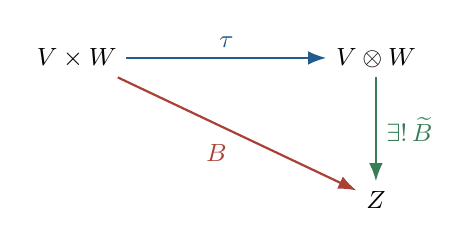
\begin{tikzpicture}[>=Latex, every node/.style={font=\small}]
 \node (vw) at (0,1.8) {$V\times W$};
 \node (tensor) at (3.8,1.8) {$V\otimes W$};
 \node (z) at (3.8,0) {$Z$};
 \draw[->,thick,manifoldblue] (vw) -- node[above] {$\tau$} (tensor);
 \draw[->,thick,manifoldred] (vw) -- node[below left] {$B$} (z);
 \draw[->,thick,manifoldgreen] (tensor) -- node[right] {$\exists!\,\widetilde B$} (z);
\end{tikzpicture}
\end{center}

Samo zapisanie $v\otimes w$ nie jest definicją: najpierw trzeba
wykazać, że przestrzeń o tej własności istnieje.

\begin{uwaga}[Co znaczy ,,formalna kombinacja liniowa''?]
\label{rem:kombinacje-formalne}
Jeśli $S$ jest dowolnym zbiorem, \emph{wolna przestrzeń liniowa}
o bazie symboli $[s]$, $s\in S$, składa się z zapisów
\[
 \sum_{s\in S} c_s[s],\qquad c_s\in\mathbb K,
 \quad c_s=0\text{ poza skończoną liczbą indeksów}.
\]
To jest kombinacja \emph{formalna}: dodajemy współczynniki
stojące przy tym samym symbolu i mnożymy je przez skalary,
ale nie przypisujemy symbolom żadnych innych relacji.
Dwa takie zapisy są równe dokładnie wtedy, gdy ich
współczynniki przy każdym $[s]$ są równe. W szczególności
$[s]$ i $[s']$ są niezależnymi wektorami, jeśli $s\ne s'$.
Można myśleć o takim zapisie jako o funkcji
$s\mapsto c_s$ o \emph{skończonym nośniku}.

W dowodzie poniżej bierzemy $S=V\times W$. Jeśli
$v,v'$ są niezależne, symbole $[(v+v',w)]$, $[(v,w)]$
i $[(v',w)]$ mają różne indeksy, więc przed podzieleniem
przez relacje są niezależne. Dopiero iloraz nakazuje równość
$[(v+v',w)]+R=[(v,w)]+[(v',w)]+R$.
Równość dwóch klas $x+R=y+R$ oznacza dokładnie $x-y\in R$.
Ta ostatnia reguła wyjaśnia, dlaczego relacje dwuliniowości
pojawiają się w konstruowanej przestrzeni, a nie były
ukrytym założeniem o symbolach.
\end{uwaga}

\begin{twierdzenie}[Konstrukcja iloczynu tensorowego]
\label{thm:tensor-istnienie}
Dla dowolnych przestrzeni liniowych $V,W$ iloczyn tensorowy istnieje.
Ponadto tensory proste rozpinają $V\otimes W$.
\end{twierdzenie}
\begin{proof}
Niech $F$ będzie wolną przestrzenią liniową o bazie formalnych
symboli $[(v,w)]$, po jednym dla każdej pary $(v,w)\in V\times W$.
Jej elementy są kombinacjami z Uwagi~\ref{rem:kombinacje-formalne}.
Ta pomocnicza przestrzeń jest na ogół nieskończenie wymiarowa,
nawet gdy $V,W$ mają skończony wymiar; dopiero iloraz narzuci relacje.
Niech $R\subseteq F$ będzie podprzestrzenią rozpiętą przez
wszystkie elementy czterech rodzajów:
\begin{align*}
 &[(v+v',w)]-[(v,w)]-[(v',w)],
 &&[(av,w)]-a[(v,w)],\\
 &[(v,w+w')]-[(v,w)]-[(v,w')],
 &&[(v,aw)]-a[(v,w)],
\end{align*}
gdzie $a\in\mathbb K$. Kładziemy $T:=F/R$ oraz
$v\otimes w:=[(v,w)]+R$. Cztery relacje pokazują kolejno,
że $\tau(v,w):=v\otimes w$ jest liniowa w każdej zmiennej.
Każda klasa w $F/R$ jest skończoną kombinacją liniową klas $[(v,w)]+R$,
więc tensory proste rozpinają $T$.

Weźmy teraz dowolne odwzorowanie dwuliniowe $B\colon V\times W\to Z$.
Na $F$ istnieje dokładnie jedno odwzorowanie liniowe
$L\colon F\to Z$ o wartościach $L([(v,w)])=B(v,w)$:
określamy je na bazie i przedłużamy liniowo. Dwuliniowość $B$
oznacza, że $L$ zeruje każdy z czterech typów generatorów $R$,
a więc $R\subseteq\ker L$. Odwzorowanie $L$ przechodzi na iloraz:
$\widetilde B(x+R):=L(x)$ dla $x\in F$. Jest dobrze określone, bo
$x+R=x'+R$ implikuje $L(x-x')=0$, i spełnia
$\widetilde B(v\otimes w)=B(v,w)$. Jeśli drugie odwzorowanie liniowe
spełniałoby tę samą równość, zgadzałoby się z $\widetilde B$
na zbiorze rozpinającym $T$, a zatem wszędzie.
\end{proof}

\begin{uwaga}[Faktoryzacja przez iloraz a izomorfizm]
\label{rem:tensor-iloraz-izomorfizm}
W dowodzie wystarczyło $R\subseteq\ker L$, aby otrzymać
odwzorowanie $\widetilde B:F/R\to Z$. To jest ten sam mechanizm
przechodzenia do ilorazu, który w ogólnej postaci
porządkuje Twierdzenie~\ref{thm:modul-izomorfizm}
w Rozdziale~\ref{ch:algebra-abstrakcyjna}
(przestrzenie liniowe są modułami nad $\mathbb K$).
Pełne twierdzenie daje $F/\ker L\cong\operatorname{im}L$.
Nie utożsamiamy natomiast $F/R$ z $\operatorname{im}L$,
chyba że $R=\ker L$; do istnienia iloczynu tensorowego
taka równość nie jest potrzebna.
\end{uwaga}

\begin{twierdzenie}[Jednoznaczność]
\label{thm:tensor-jednoznacznosc}
Jeżeli $(T,\tau)$ i $(T',\tau')$ spełniają
Definicję~\ref{def:tensor-universal}, istnieje dokładnie jeden
izomorfizm spełniający
\[
 J\colon T\to T',\qquad J\circ\tau=\tau'.
\]
\end{twierdzenie}
\begin{proof}
Własność uniwersalna $(T,\tau)$ zastosowana do $\tau'$ daje
jedyne odwzorowanie liniowe $J\colon T\to T'$ z~żądaną własnością.
Podobnie $(T',\tau')$ daje $K\colon T'\to T$ z
$K\circ\tau'=\tau$. Zatem $(KJ)\circ\tau=\tau$.
Również $\id_T\circ\tau=\tau$; jednoznaczność faktoryzacji
przez $T$ wymusza $KJ=\id_T$. Tak samo $JK=\id_{T'}$.
Odwzorowanie $J$ jest więc izomorfizmem i jedynym możliwym odwzorowaniem
zachowującym wskazane obrazy par $(v,w)$.
\end{proof}

W szczególności
\begin{equation}\label{eq:tensor-biliniowosc}
 (av+bv')\otimes w=a(v\otimes w)+b(v'\otimes w),\qquad
 v\otimes(aw+bw')=a(v\otimes w)+b(v\otimes w').
\end{equation}
\emph{Każdy} element $V\otimes W$ jest skończoną sumą tensorów
prostych, ale nie musi sam być tensorem prostym.

\section{Baza, wymiar i wiele czynników}
\label{sec:baza-tensorowa}

\begin{twierdzenie}[Baza iloczynu tensorowego]
\label{thm:baza-tensorowa}
Jeżeli $e_1,\ldots,e_m$ jest bazą $V$, a
$f_1,\ldots,f_n$ bazą $W$, to
\[
 \bigl\{e_i\otimes f_j:1\leq i\leq m,\;1\leq j\leq n\bigr\}
\]
jest bazą $V\otimes W$. W szczególności
$\dim(V\otimes W)=mn$.
\end{twierdzenie}
\begin{proof}
Dla $v=\sum_i a_i e_i$ i $w=\sum_j b_j f_j$ dwuliniowość daje
\[
 v\otimes w=\sum_{i=1}^m\sum_{j=1}^n a_ib_j(e_i\otimes f_j).
\]
Ponieważ tensory proste rozpinają $V\otimes W$, wyświetlone
wektory są układem rozpinającym. Dla liniowej niezależności
wprowadźmy przestrzeń $\mathbb K^{m\times n}$ z bazą jednostek
macierzowych $E_{ij}$: jedynka na miejscu $(i,j)$ i zera poza nim. Przypisanie
$B(v,w)=(a_i b_j)_{i,j}$ jest dwuliniowe; własność uniwersalna
daje $\widetilde B\colon V\otimes W\to\mathbb K^{m\times n}$
z $\widetilde B(e_i\otimes f_j)=E_{ij}$. Jeśli
$\sum_{i,j}c_{ij}e_i\otimes f_j=0$, zastosowanie
$\widetilde B$ daje $\sum_{i,j}c_{ij}E_{ij}=0$, czyli
wszystkie $c_{ij}=0$. Tak wykazaliśmy również podany wymiar.
\end{proof}

\begin{przyklad}[Tensor prosty a suma tensorów]
Dla $V=W=\R^2$ odwzorowanie z dowodu przypisuje
$(1,2)\otimes(3,-1)$ macierz
$\begin{psmallmatrix}3&-1\\6&-2\end{psmallmatrix}$.
Każdy niezerowy tensor prosty ma tu macierz rzędu $1$:
jest ona iloczynem kolumny współrzędnych $v$ i wiersza
współrzędnych $w$. Natomiast
$e_1\otimes e_1+e_2\otimes e_2$ odpowiada macierzy
identycznościowej rzędu $2$, więc nie jest prosty.
Należy też pamiętać, że $v\otimes w$ nie oznacza pary $(v,w)$:
na przykład $(2v)\otimes w=v\otimes(2w)$.
\end{przyklad}

\begin{stwierdzenie}[Łączność i przestawianie czynników]
\label{prop:tensor-lacznosc}
Istnieją kanoniczne izomorfizmy
\[
 (V\otimes W)\otimes U\longrightarrow V\otimes(W\otimes U),
 \quad (v\otimes w)\otimes u\longmapsto v\otimes(w\otimes u),
\]
\[
 V\otimes W\longrightarrow W\otimes V,
 \quad v\otimes w\longmapsto w\otimes v.
\]
Dlatego możemy pisać $V_1\otimes\cdots\otimes V_k$ bez nawiasów.
\end{stwierdzenie}
\begin{proof}
Odwzorowanie $(v,w,u)\mapsto v\otimes(w\otimes u)$ jest
trójliniowe. Każde odwzorowanie trójliniowe na $V\times W\times U$
faktoryzuje jednoznacznie przez $(V\otimes W)\otimes U$:
najpierw przy ustalonym $u$ faktoryzujemy względem $(v,w)$;
otrzymane odwzorowania $(V\otimes W)\to Z$ zależą liniowo od $u$,
co sprawdzamy na rozpinających $v\otimes w$. Następnie
faktoryzujemy powstałe odwzorowanie dwuliniowe
$(V\otimes W)\times U\to Z$. Otrzymujemy zatem odwzorowanie w treści
stwierdzenia. Analogiczna konstrukcja w drugą stronę daje
$v\otimes(w\otimes u)\mapsto(v\otimes w)\otimes u$.
Oba złożenia są identycznością na tensorach prostych trzech
czynników, które rozpinają odpowiednie przestrzenie.
Izomorfizm przestawiający dwa czynniki pochodzi z dwuliniowego
odwzorowania $(v,w)\mapsto w\otimes v$; jego odwrotność powstaje
po ponownym przestawieniu.
Przy większej liczbie czynników dowolne dwa sposoby zmiany
nawiasowania dają to samo odwzorowanie: na każdym tensorze
prostym zachowują kolejność i wartości wszystkich czynników,
a takie tensory rozpinają dziedzinę. To uzasadnia pomijanie
nawiasów również dla czterech i więcej przestrzeni.
\end{proof}

Kładziemy $V^{\otimes0}:=\mathbb K$ oraz
$V^{\otimes k}:=V\otimes\cdots\otimes V$ dla $k\geq1$.
Jeżeli $\dim V=n$, iterowanie Twierdzenia~\ref{thm:baza-tensorowa}
daje bazę $e_{i_1}\otimes\cdots\otimes e_{i_k}$ i wymiar
\begin{equation}\label{eq:dim-potega-tensorowa}
 \dim V^{\otimes k}=n^k\qquad(k\geq0).
\end{equation}
Dla $k=0$ jest to konwencja $n^0=1$, również gdy $V=0$.

\section{Tensory mieszane i operacje na nich}
\label{sec:operacje-tensorowe}

Oznaczmy $V^*:=\operatorname{Hom}_{\mathbb K}(V,\mathbb K)$.
Jest to przestrzeń liniowych funkcjonałów, zwanych kowektorami.
Dla nieujemnych $r,s$ przyjmujemy konwencję
\begin{equation}\label{eq:typ-tensora}
 T^r_s(V):=V^{\otimes r}\otimes(V^*)^{\otimes s}.
\end{equation}
Tensory typu $(r,s)$ mają $r$ czynników wektorowych i $s$
kowektorowych; powiązane z nimi funkcje wieloliniowe
przyjmują $r$ kowektorów i $s$ wektorów. Na tensorze prostym
wyznacza je wzór
\[
 (v_1\otimes\cdots\otimes v_r\otimes
 \alpha_1\otimes\cdots\otimes\alpha_s)
 (\xi_1,\ldots,\xi_r;w_1,\ldots,w_s)
 =\prod_{a=1}^r\xi_a(v_a)\prod_{b=1}^s\alpha_b(w_b).
\]
Puste iloczyny mają wartość $1$. Dla $r=s=0$ mamy
$T^0_0(V)=\mathbb K$; odwzorowanie bez argumentów określa po prostu
skalar (dziedziną jest jednoelementowy zbiór pustych układów).

\begin{twierdzenie}[Postać wieloliniowa tensora]
\label{thm:tensor-wieloliniowy}
Dla skończenie wymiarowej przestrzeni $V$ powyższy wzór daje
izomorfizm
\[
 T^r_s(V)\cong
 \operatorname{Mult}\bigl((V^*)^r\times V^s,\mathbb K\bigr).
\]
Jeśli $e_1,\ldots,e_n$ jest bazą $V$ i $e^1,\ldots,e^n$
bazą dualną, każdy tensor ma dokładnie jedno rozwinięcie
\begin{equation}\label{eq:wspolczynniki-tensora}
 T=\sum_{\substack{i_1,\ldots,i_r\\j_1,\ldots,j_s}}
 T^{i_1\cdots i_r}{}_{j_1\cdots j_s}
 e_{i_1}\otimes\cdots\otimes e_{i_r}
 \otimes e^{j_1}\otimes\cdots\otimes e^{j_s}.
\end{equation}
\end{twierdzenie}
\begin{proof}
Rozwinięcie i jego jednoznaczność wynikają z kolejnych
zastosowań Twierdzenia~\ref{thm:baza-tensorowa}. Wzór
na działanie na argumentach jest wieloliniowy w czynnikach
tensora, więc przez własność uniwersalną definiuje odwzorowanie liniowe
$T^r_s(V)$ do wskazanej przestrzeni funkcji. Aby wykazać jego
iniektywność, podstawmy w miejsce argumentów elementy baz:
\[
 e^{i_1},\ldots,e^{i_r};\qquad e_{j_1},\ldots,e_{j_s}.
\]
Uzyskana wartość jest dokładnie współczynnikiem
$T^{i_1\cdots i_r}{}_{j_1\cdots j_s}$. Jeśli wszystkie wartości
są zerowe, znikają więc wszystkie współczynniki.
Odwrotnie, dla dowolnej funkcji wieloliniowej $F$ wstawmy te
wartości do prawej strony~\eqref{eq:wspolczynniki-tensora}.
Otrzymany tensor ma te same wartości co $F$ na wszystkich
układach elementów bazowych. Rozwinięcie argumentów i ich
wieloliniowość dają równość na dowolnych argumentach.
\end{proof}

Przykładowo $T^0_2(V)$ to formy dwuliniowe na $V$.
Związek tensorów z operatorami wymaga pilnowania,
z której przestrzeni operator \emph{przyjmuje} argument.

\begin{twierdzenie}[Tensory i przestrzenie operatorów]
\label{thm:tensor-hom}
Dla skończenie wymiarowych $V,W$ istnieje kanoniczny izomorfizm
\begin{equation}\label{eq:tensor-hom}
 \Theta_{V,W}\colon V\otimes W^*\longrightarrow
 \operatorname{Hom}_{\mathbb K}(W,V),\qquad
 \Theta_{V,W}(v\otimes\lambda)(w):=\lambda(w)v.
\end{equation}
W szczególności po zamianie nazw przestrzeni otrzymujemy
$W\otimes V^*\cong\operatorname{Hom}_{\mathbb K}(V,W)$.
\end{twierdzenie}
\begin{proof}
Dla ustalonego $w\in W$ wyrażenie $\lambda(w)v$ zależy
liniowo od $v$ oraz liniowo od $\lambda$; samo przypisanie
$w\mapsto\lambda(w)v$ jest liniowe. Dlatego odwzorowanie
$(v,\lambda)\mapsto(w\mapsto\lambda(w)v)$ ma wartości
w $\operatorname{Hom}(W,V)$ i jest dwuliniowe.
Własność uniwersalna iloczynu tensorowego wyznacza
\emph{jedno} odwzorowanie liniowe $\Theta_{V,W}$ o wzorze
\eqref{eq:tensor-hom}. Tym samym wzór działa również
na sumach: $\Theta_{V,W}(\sum_a v_a\otimes\lambda_a)(w)
=\sum_a\lambda_a(w)v_a$. Nie musimy wybierać sposobu
zapisania takiej sumy, bo $\Theta_{V,W}$ została zdefiniowana
na całej przestrzeni tensorowej.

Zbudujmy odwrotność. Wybierzmy bazę $f_1,\ldots,f_m$
przestrzeni $W$ i jej bazę dualną $f^1,\ldots,f^m$.
Dla $A\in\operatorname{Hom}(W,V)$ połóżmy
\begin{equation}\label{eq:hom-tensor-odwrotna}
 \mathcal I(A):=\sum_{j=1}^m A(f_j)\otimes f^j\in V\otimes W^*.
\end{equation}
Sprawdzimy oba złożenia. Jeśli $w\in W$, to
\[
 \Theta_{V,W}(\mathcal I(A))(w)
 =\sum_j f^j(w)A(f_j)
 =A\!\left(\sum_j f^j(w)f_j\right)=A(w),
\]
bo $w=\sum_j f^j(w)f_j$. Odwrotnie, dla prostego
tensora $v\otimes\lambda$ mamy
\[
 \mathcal I(\Theta_{V,W}(v\otimes\lambda))
 =\sum_j\lambda(f_j)v\otimes f^j
 =v\otimes\left(\sum_j\lambda(f_j)f^j\right)
 =v\otimes\lambda.
\]
Tensory proste rozpinają $V\otimes W^*$, więc drugie
złożenie też jest identycznością wszędzie. Wzór
\eqref{eq:hom-tensor-odwrotna} wygląda zależnie od bazy,
ale jest odwrotnością kanonicznej $\Theta_{V,W}$;
dlatego jego wynik od bazy nie zależy.
\end{proof}

Przy $W=V$ otrzymujemy
$T^1_1(V)=V\otimes V^*\cong\operatorname{End}(V)$.
Na tensorze prostym odpowiada temu wzór
\begin{equation}\label{eq:endo-tensor}
 v\otimes\alpha\longmapsto
 \bigl(w\longmapsto\alpha(w)v\bigr).
\end{equation}
Na przykład $e_i\otimes e^j$ przechodzi na jednostkę
macierzową $E_{ij}$: wysyła $e_j$ na $e_i$, a pozostałe
wektory bazowe na zero. W bazie $e'_i=\sum_a A^a{}_i e_a$
macierz operatora $S$ ma postać $[S]'=A^{-1}[S]A$:
zmieniają się współczynniki, nie sam operator.
Istotnie, jeśli $[v]$ i $[v]'$ oznaczają kolumny współrzędnych,
to $[v]=A[v]'$. Stąd $[Sv]'=A^{-1}[S]A[v]'$.
Baza dualna zmienia się według
$e'^i=\sum_b(A^{-1})^i{}_b e^b$, co wynika z warunku
$e'^i(e'_j)=\delta^i_j$; używamy odwrotności bez sprzężenia zespolonego.

\begin{uwaga}[Funkcja dwuliniowa a operator]
\label{rem:mult-hom}
Z Twierdzenia~\ref{thm:tensor-wieloliniowy} dla typu $(1,1)$
dostajemy
\[
 V\otimes V^*\cong\operatorname{Mult}(V^*\times V,\mathbb K).
\]
Dlaczego równie często spotyka się zapis
$\operatorname{Mult}(V\times V^*,\mathbb K)$?
Kolejność argumentów można po prostu zamienić: jeśli
$C(\lambda,v)$ jest dwuliniowa, to $B(v,\lambda):=C(\lambda,v)$
też jest dwuliniowa. Jest to odwracalna operacja, niezależna
od wyboru bazy. W obu zapisach odpowiadający operatorowi
$A\in\operatorname{Hom}(V,V)$ wzór ma postać
\begin{equation}\label{eq:mult-operator}
 B_A(v,\lambda)=\lambda(Av),
 \qquad v\in V,\quad\lambda\in V^*.
\end{equation}
Wektor $v$ jest argumentem operatora $A$; kowektor
$\lambda$ odczytuje liczbę z wyniku $Av$.

Sprawdźmy, że przy $\dim V<\infty$ wzór ten obejmuje
\emph{każdą} taką funkcję dwuliniową $B$. Wybierzmy bazę
$e_1,\ldots,e_n$ i bazę dualną $e^1,\ldots,e^n$, po czym
zdefiniujmy
\[
 A_B(v):=\sum_{i=1}^n B(v,e^i)e_i.
\]
Odwzorowanie $A_B$ jest liniowe, bo $B$ jest liniowa w pierwszym
argumencie. Dla dowolnego $\lambda\in V^*$ zachodzi
\[
 \lambda(A_Bv)=\sum_i B(v,e^i)\lambda(e_i)
 =B\!\left(v,\sum_i\lambda(e_i)e^i\right)=B(v,\lambda).
\]
Jeżeli dwa operatory dają tę samą funkcję $B$, każdy kowektor
przyjmuje na ich wartościach ten sam wynik, więc operatory
są równe. Zatem
$\operatorname{Mult}(V\times V^*,\mathbb K)
 \cong\operatorname{Hom}(V,V)$.
Na przykład tensor $u\otimes\alpha$ odpowiada operatorowi
$A(v)=\alpha(v)u$, a następnie funkcji
$B_A(v,\lambda)=\alpha(v)\lambda(u)$.
Nie utożsamiamy przy tym $V$ z $V^*$; korzystamy jedynie
z naturalnego sparowania $\lambda(v)$.
\end{uwaga}

\begin{przyklad}[Tensor prosty i nieprosty typu $(1,1)$]
Niech $V=\R^2$, niech $e_1,e_2$ będzie jego bazą, a
$e^1,e^2$ bazą dualną. Tensor
\[
 P=(e_1+e_2)\otimes(e^1-e^2)
\]
jest \emph{prosty}: ma postać jednego iloczynu tensorowego.
Odpowiada mu operator $A_P(v)=(e^1(v)-e^2(v))(e_1+e_2)$,
o macierzy
$\begin{psmallmatrix}1&-1\\1&-1\end{psmallmatrix}$.
Wszystkie jego wartości leżą na jednej prostej, więc
$\operatorname{rank}A_P=1$. Jego funkcja dwuliniowa to
$B_P(v,\lambda)=(e^1(v)-e^2(v))\lambda(e_1+e_2)$.

Z kolei tensor
$Q=e_1\otimes e^1+e_2\otimes e^2$ jest
\emph{nieprosty}. Odpowiada mu operator
$A_Q(v)=e^1(v)e_1+e^2(v)e_2=v$, czyli macierz
$\begin{psmallmatrix}1&0\\0&1\end{psmallmatrix}$ i funkcja
$B_Q(v,\lambda)=\lambda(v)$. Gdyby $Q=u\otimes\alpha$,
obraz $A_Q$ mieściłby się w prostej $\mathbb Ku$.
Jednak $A_Q(e_1)=e_1$ i $A_Q(e_2)=e_2$ są niezależne;
stąd $Q$ nie może być jednym tensorem prostym.
\end{przyklad}

\begin{uwaga}[Kolejność czynników jest istotna]
Równość $V\otimes W^*\cong\operatorname{Hom}(V,W)$
nie jest naturalnym utożsamieniem: wzór~\eqref{eq:tensor-hom}
przyjmuje argument $w\in W$ i zwraca wynik w $V$.
Do otrzymania odwzorowań z $V$ do $W$ trzeba wziąć
$W\otimes V^*$. Przestrzenie $V\otimes W^*$ oraz
$\operatorname{Hom}(V,W)$ mają wprawdzie równy wymiar,
ale równość wymiarów daje jedynie istnienie pewnego
izomorfizmu po dokonaniu dodatkowych wyborów, np.\ baz.
\end{uwaga}

\begin{twierdzenie}[Iloczyn tensorowy odwzorowań]
\label{thm:tensor-operatorow}
Dla odwzorowań liniowych $A\colon V\to V'$ i $B\colon W\to W'$
istnieje dokładnie jedno odwzorowanie liniowe
$A\otimes B\colon V\otimes W\to V'\otimes W'$ spełniające
\begin{equation}\label{eq:tensor-operatorow}
 (A\otimes B)(v\otimes w)=Av\otimes Bw.
\end{equation}
Jeżeli $A'\colon V'\to V''$ i $B'\colon W'\to W''$, to
\[
 (A'\otimes B')\circ(A\otimes B)=(A'\circ A)\otimes(B'\circ B),
 \qquad \id_V\otimes\id_W=\id_{V\otimes W}.
\]
Dla przestrzeni skończenie wymiarowych
$\operatorname{rank}(A\otimes B)=\operatorname{rank}A\,\operatorname{rank}B$.
\end{twierdzenie}
\begin{proof}
Odwzorowanie $(v,w)\mapsto Av\otimes Bw$ jest dwuliniowe:
liniowość $A$ i pierwszego miejsca $\otimes$ dają
liniowość w $v$, analogicznie w $w$. Własność uniwersalna
tworzy dokładnie jedno odwzorowanie o wzorze~\eqref{eq:tensor-operatorow}.
Obie strony równości złożeń przyłożone do $v\otimes w$
dają $A'Av\otimes B'Bw$. Tensory proste rozpinają dziedzinę,
więc odwzorowania są równe. Identyczność sprawdzamy tak samo.

Obraz $A\otimes B$ jest rozpięty przez wszystkie $Av\otimes Bw$,
więc równa się $(\operatorname{im}A)\otimes(\operatorname{im}B)$,
rozumianemu jako podprzestrzeń $V'\otimes W'$.
Aby uzasadnić to ostatnie włączenie bez ukrytego założenia,
dopełnijmy bazy obu obrazów do baz $V'$ i $W'$;
Twierdzenie~\ref{thm:baza-tensorowa} pokazuje, że iloczyny
wektorów z mniejszych baz pozostają liniowo niezależne
w większym iloczynie tensorowym. Ich liczba to iloczyn rang.
\end{proof}

Jeśli macierze $A,B$ mają współczynniki $a_{pi},b_{qj}$,
to w bazach $e_i\otimes f_j$ współczynnik macierzy
$A\otimes B$ o indeksach $(p,q),(i,j)$ jest $a_{pi}b_{qj}$.
Jest to \emph{iloczyn Kroneckera}. Pary porządkujemy
leksykograficznie: $(1,1),(1,2),\ldots,(2,1),\ldots$.
W takim porządku na przykład
\[
 A=\begin{pmatrix}1&2\\0&1\end{pmatrix},\quad
 B=\begin{pmatrix}2&0\\0&3\end{pmatrix},\qquad
 A\otimes B=
 \begin{pmatrix}
 2&0&4&0\\0&3&0&6\\0&0&2&0\\0&0&0&3
 \end{pmatrix}.
\]

Iloczyn tensorów mieszanych wymaga ustalenia kolejności.
Jeśli $S\in T^r_s(V)$ i $T\in T^{r'}_{s'}(V)$, ich surowy
iloczyn ma kolejno bloki $V^{\otimes r}$, $(V^*)^{\otimes s}$,
$V^{\otimes r'}$, $(V^*)^{\otimes s'}$. Przenosimy trzeci blok
przed drugi kanonicznym przestawieniem czynników i tak otrzymany
element $T^{r+r'}_{s+s'}(V)$ oznaczamy także $S\otimes T$.
Wewnątrz bloków zachowujemy kolejność. Nie pojawia się znak:
jest to zwykły iloczyn tensorowy, a nie iloczyn zewnętrzny.

\begin{definicja}[Kontrakcja]
\index{kontrakcja@Kontrakcja}
\label{def:kontrakcja}
\emph{Kontrakcja} usuwa jedną parę: czynnik $V$ i czynnik $V^*$,
łącząc je przez ewaluację $\alpha(v)$. W najprostszym przypadku
jest to odwzorowanie $C\colon V\otimes V^*\to\mathbb K$,
$C(v\otimes\alpha)=\alpha(v)$. W~ogólności dostajemy
$C_{a,b}\colon T^r_s(V)\to T^{r-1}_{s-1}(V)$, gdy $r,s\geq1$.
Indeksy spełniają $1\leq a\leq r$ i $1\leq b\leq s$.
Na tensorze prostym mnożymy przez $\alpha_b(v_a)$,
usuwamy czynniki $v_a$ i $\alpha_b$, a pozostałe zachowujemy
w pierwotnej kolejności. Przykładowo kontrakcja pierwszej pary ma współczynniki
\[
 (C_{1,1}T)^{i_2\cdots i_r}{}_{j_2\cdots j_s}
 =\sum_{a=1}^{\dim V}T^{a i_2\cdots i_r}{}_{a j_2\cdots j_s}.
\]
\end{definicja}

\begin{stwierdzenie}[Kontrakcja i ślad]
\label{prop:kontrakcja-slad}
Kontrakcja jest liniowa i nie zależy od wyboru bazy. Dla
$S=\sum_{i,j}S^i{}_j e_i\otimes e^j\in T^1_1(V)$ zachodzi
\[
 C(S)=\sum_i S^i{}_i=\operatorname{tr}S,
\]
gdzie ostatni ślad dotyczy operatora z~\eqref{eq:endo-tensor}.
\end{stwierdzenie}
\begin{proof}
Ewaluacja $(v,\alpha)\mapsto\alpha(v)$ jest dwuliniowa,
więc ma jednoznaczne przedłużenie do $V\otimes V^*$.
Pozostałe czynniki przestawiamy izomorfizmami ze
Stwierdzenia~\ref{prop:tensor-lacznosc} i stosujemy tę ewaluację
w wybranej parze. Ponieważ definicja używa jedynie wartości
kowektora na wektorze, wynik nie zależy od bazy.
Dla współrzędnych $C(e_i\otimes e^j)=e^j(e_i)=\delta_i^j$,
więc $C(S)=\sum_i S^i{}_i$. Z~\eqref{eq:endo-tensor}
współczynniki $S^i{}_j$ są współczynnikami macierzy operatora,
a powyższa suma jest jej śladem.
\end{proof}

\begin{przyklad}[Iloczyn i kontrakcja]
Niech $S=e_1\otimes e^1+2e_2\otimes e^2$ na $\R^2$.
Wtedy $S(e_1)=e_1$, $S(e_2)=2e_2$, a $C(S)=3$.
Dla $u\otimes v\otimes\alpha\in T^2_1(V)$ kontrakcja
$v$ z $\alpha$ daje $\alpha(v)u$, zaś kontrakcja
$u$ z $\alpha$ daje $\alpha(u)v$. Wybór pary ma znaczenie.
\end{przyklad}

\section{Algebra tensorowa i symetryzacja}
\label{sec:algebra-tensorowa}

Wyjaśnijmy użyte dalej słowa. \emph{Algebra} to przestrzeń
liniowa z dwuliniowym mnożeniem; u nas mnożenie będzie
łączne i będzie miało element jednostkowy $1$.
\emph{Suma prosta} $\bigoplus_{k\geq0}U_k$ zawiera ciągi
$(u_0,u_1,\ldots)$ z tylko skończenie wieloma niezerowymi
składnikami. \emph{Ideał obustronny} $I$ algebry $A$ to
podprzestrzeń taka, że $ai,ia\in I$ dla wszystkich
$a\in A$, $i\in I$. Dzięki temu na klasach w $A/I$
można określić mnożenie $(a+I)(b+I)=ab+I$:
zamiana $a$ na $a+i$ i $b$ na $b+j$ dodaje do
iloczynu wyrazy $aj+ib+ij\in I$. Algebra jest
\emph{stopniowana}, gdy $A=\bigoplus_{k\geq0}A^k$
i $A^kA^\ell\subseteq A^{k+\ell}$. Element należący do $A^k$ nazywamy
jednorodnym stopnia $k$. Homomorfizm algebr z jedynką to
odwzorowanie liniowe zachowujące mnożenie i jedynkę.

\begin{samepage}
\begin{definicja}[Algebra tensorowa]
\index{algebra tensorowa@Algebra tensorowa}
\label{def:algebra-tensorowa}
\emph{Algebra tensorowa} przestrzeni $V$ to suma prosta
\[
 T(V):=\bigoplus_{k=0}^{\infty}V^{\otimes k},
 \qquad V^{\otimes0}=\mathbb K.
\]
Elementy tej sumy mają tylko skończenie wiele niezerowych
składników. Mnożenie tensorów jednorodnych definiujemy przez
\emph{konkatenację}:
\[
 (v_1\otimes\cdots\otimes v_k)
 \cdot(w_1\otimes\cdots\otimes w_\ell)
 :=v_1\otimes\cdots\otimes v_k\otimes w_1\otimes\cdots\otimes w_\ell.
\]
Rozszerzamy je dwuliniowo na $T(V)$; jedynką jest $1\in\mathbb K$.
W stopniu $0$ mnożenie jest zwykłym mnożeniem przez skalar.
Definicja na tensorach prostych przechodzi na całe potęgi tensorowe
dzięki iterowanej własności uniwersalnej: jest liniowa w każdym
czynniku. Skończoność nośnika sum zapewnia, że wynik znów należy do $T(V)$.
\end{definicja}
\end{samepage}

\begin{twierdzenie}[Łączność i swoboda algebry tensorowej]
\label{thm:algebra-tensorowa-universal}
$T(V)$ jest łączną algebrą z jedynką, na ogół nieprzemienną.
Dla każdej łącznej algebry $\mathcal A$ z jedynką i każdego
odwzorowania liniowego $f\colon V\to\mathcal A$ istnieje dokładnie jeden
homomorfizm algebr z jedynką $\widehat f\colon T(V)\to\mathcal A$
spełniający $\widehat f|_V=f$.
\end{twierdzenie}
\begin{proof}
Na tensorach prostych obu stron równości
$(ab)c=a(bc)$ otrzymujemy ten sam tensor przez zapisanie
wszystkich czynników po kolei. Stwierdzenie~\ref{prop:tensor-lacznosc}
pozwala pominąć nawiasy; dwuliniowość rozszerza równość
na sumy skończone. Podobnie $1\cdot a=a\cdot1=a$.

Dla ustalonego $k\geq1$ odwzorowanie
$(v_1,\ldots,v_k)\mapsto f(v_1)\cdots f(v_k)$
jest $k$-liniowe, ponieważ mnożenie w $\mathcal A$ jest
dwuliniowe. Iterowana własność uniwersalna daje jedyne odwzorowanie
liniowe $f_k\colon V^{\otimes k}\to\mathcal A$ spełniające
$f_k(v_1\otimes\cdots\otimes v_k)=f(v_1)\cdots f(v_k)$.
W stopniu $0$ kładziemy $f_0(a)=a1_{\mathcal A}$.
Definiujemy $\widehat f$ na całej sumie prostej jako sumę
$f_k$ po jej skończenie wielu niezerowych składowych.
Dla tensorów prostych zachodzi
$\widehat f(a\cdot b)=\widehat f(a)\widehat f(b)$;
dwuliniowość dowodzi tego dla dowolnych $a,b$.
Jedynka też jest zachowana. Jeśli $g$ jest drugim takim
homomorfizmem, to na $v_1\otimes\cdots\otimes v_k$
musi przyjmować wartość $g(v_1)\cdots g(v_k)
=f(v_1)\cdots f(v_k)$; te tensory i $1$ rozpinają $T(V)$.
Stąd $g=\widehat f$.
\end{proof}

Dla niezależnych $e_1,e_2$ tensory $e_1\otimes e_2$ i
$e_2\otimes e_1$ są różnymi elementami $V^{\otimes2}$.
Wymuszenie przemienności prowadzi do algebry symetrycznej,
a wymuszenie $v\wedge v=0$ do algebry zewnętrznej.

\begin{definicja}[Symetryzator i antysymetryzator]
\index{symetryzator i antysymetryzator@Symetryzator i antysymetryzator}
\label{def:sym-alt}
Dla $k\geq1$ permutacja $\sigma\in S_k$ działa na
$V^{\otimes k}$ przez
\[
 P_\sigma(v_1\otimes\cdots\otimes v_k)
 :=v_{\sigma^{-1}(1)}\otimes\cdots\otimes v_{\sigma^{-1}(k)}.
\]
Odwzorowania te istnieją na mocy iterowanej własności uniwersalnej.
Definiujemy projekcje
\begin{equation}\label{eq:sym-alt}
 \operatorname{Sym}_k:=\frac1{k!}\sum_{\sigma\in S_k}P_\sigma,
 \qquad
 \operatorname{Alt}_k:=\frac1{k!}\sum_{\sigma\in S_k}
\operatorname{sgn}(\sigma)P_\sigma.
\end{equation}
W stopniu $0$ przyjmujemy
$\operatorname{Sym}_0=\operatorname{Alt}_0=\id_{\mathbb K}$.
\end{definicja}

\begin{twierdzenie}[Własności obu projekcji]
\label{thm:sym-alt}
Dla $t\in V^{\otimes k}$ zachodzi
\[
 \operatorname{Sym}_k^2=\operatorname{Sym}_k,\qquad
 \operatorname{Alt}_k^2=\operatorname{Alt}_k,
\]
a ich obrazy są dokładnie przestrzeniami tensorów spełniających,
odpowiednio, $P_\sigma t=t$ albo
$P_\sigma t=\operatorname{sgn}(\sigma)t$ dla każdego $\sigma$.
\end{twierdzenie}
\begin{proof}
Dzięki wyborowi $\sigma^{-1}$ w definicji
$P_\sigma P_\tau=P_{\sigma\tau}$; sprawdzamy to bezpośrednio
na tensorach prostych. Dla ustalonej $\tau$ podstawienie
$\rho=\tau\sigma$ w sumach~\eqref{eq:sym-alt} daje
\[
 P_\tau\operatorname{Sym}_k=\operatorname{Sym}_k,
 \qquad
 P_\tau\operatorname{Alt}_k
 =\operatorname{sgn}(\tau)\operatorname{Alt}_k.
\]
Tak samo, zmieniając indeks po prawej stronie, otrzymujemy
$\operatorname{Sym}_kP_\tau=\operatorname{Sym}_k$ oraz
$\operatorname{Alt}_kP_\tau=\operatorname{sgn}(\tau)\operatorname{Alt}_k$.
Każdy element pierwszego obrazu jest więc niezmienniczy,
a drugiego zmienia znak zgodnie z parzystością permutacji.
Jeżeli odwrotnie $P_\sigma t=t$ dla wszystkich $\sigma$,
to $\operatorname{Sym}_k t=\frac1{k!}\sum_\sigma t=t$.
Jeśli $P_\sigma t=\operatorname{sgn}(\sigma)t$, to
$\operatorname{Alt}_k t=
\frac1{k!}\sum_\sigma\operatorname{sgn}(\sigma)^2t=t$.
Zastosowanie projekcji do jej obrazu nic więc nie zmienia,
co daje obie równości idempotencji.
\end{proof}

Na przykład
\[
 \operatorname{Sym}_2(u\otimes v)
 =\tfrac12(u\otimes v+v\otimes u),\qquad
 \operatorname{Alt}_2(u\otimes v)
 =\tfrac12(u\otimes v-v\otimes u).
\]
Dla $u=v$ drugi tensor znika. W stopniu $k=1$ obie
projekcje są identycznością.

\begin{przyklad}[Rozkład tensora dwukowariantnego]
Niech $e^1,e^2$ będzie bazą $V^*$ i
$t=e^1\otimes e^2+3e^2\otimes e^1$.
Wówczas $t(e_1,e_2)=1$, $t(e_2,e_1)=3$, a
\[
 \operatorname{Sym}_2(t)
 =2(e^1\otimes e^2+e^2\otimes e^1),\qquad
 \operatorname{Alt}_2(t)
 =-e^1\otimes e^2+e^2\otimes e^1.
\]
Ich suma jest równa $t$. Pierwszy składnik jest symetryczny,
drugi zmienia znak po zamianie argumentów.
\end{przyklad}

Równość $t=\operatorname{Sym}_2t+\operatorname{Alt}_2t$
zachodzi dla każdego tensora drugiego stopnia, bo w sumie
$\tfrac12(\id+P_{(12)})+\tfrac12(\id-P_{(12)})$ zostaje $\id$.
Nie jest to ogólny rozkład na dwie części dla $k\geq3$.
Na przykład dla trzech niezależnych wektorów bazowych
współczynnik $e_1\otimes e_2\otimes e_3$ w
$(\operatorname{Sym}_3+\operatorname{Alt}_3)
(e_1\otimes e_2\otimes e_3)$ wynosi $2/6$, a nie $1$.

\begin{definicja}[Algebra symetryczna]
\index{algebra symetryczna@Algebra symetryczna}
\label{def:algebra-symetryczna}
Niech $J$ będzie obustronnym ideałem w $T(V)$ generowanym
przez wszystkie $u\otimes v-v\otimes u$. Iloraz
$S(V):=T(V)/J$ jest \emph{algebrą symetryczną}.
Jego składową stopnia $k$ oznaczamy $S^k(V)$.
Jest ona równa $V^{\otimes k}/(J\cap V^{\otimes k})$.
Istotnie, $J$ jest sumą swoich części jednorodnych:
w każdym elemencie $a(u\otimes v-v\otimes u)b$ rozwijamy
$a,b$ na skończone sumy składników jednorodnych. Każda
otrzymana część nadal należy do $J$. To uzasadnia stopniowanie ilorazu.
\end{definicja}

\begin{stwierdzenie}[Baza algebry symetrycznej]
\label{prop:sym-baza}
Dla bazy $e_1,\ldots,e_n$ i $k\geq0$ klasy
$e_1^{a_1}\cdots e_n^{a_n}$, gdzie
$a_i\geq0$ i $a_1+\cdots+a_n=k$, tworzą bazę $S^k(V)$.
Zatem
\[
 \dim S^k(V)=\binom{n+k-1}{k}\quad(n\geq1),
 \qquad S^k(V)\cong\operatorname{im}\operatorname{Sym}_k\quad(k\geq1).
\]
\end{stwierdzenie}
\begin{proof}
Niech $q\colon T(V)\to S(V)$ będzie ilorazem.
Ponieważ $q(e_i)q(e_j)=q(e_j)q(e_i)$, każdą klasę tensora
prostego można uporządkować do postaci
$e_1^{a_1}\cdots e_n^{a_n}$; te jednomiany rozpinają.
Zdefiniujmy homomorfizm $\pi\colon S(V)\to
\mathbb K[x_1,\ldots,x_n]$ przez $\pi(q(e_i))=x_i$.
Istnieje, bo odwzorowanie z algebry tensorowej wysyłające $e_i$
na $x_i$ zeruje każdy generator $J$. Z drugiej strony
przypisanie $x_i\mapsto q(e_i)$ wyznacza homomorfizm
$\rho\colon\mathbb K[x_1,\ldots,x_n]\to S(V)$:
na wielomianie podstawiamy za zmienne te przemienne elementy.
Oba złożenia ustalają wszystkie generatory i jedynkę,
więc są identycznościami. Niezależność i rozpinanie
wynikają teraz z niezależności zwykłych jednomianów.
Liczbę rozwiązań $a_1+\cdots+a_n=k$ otrzymujemy przez
rozmieszczenie $n-1$ przegród wśród $n+k-1$ pozycji,
czyli $\binom{n+k-1}{k}$.

Na koniec w stopniu $k$ zachodzi $q_kP_\sigma=q_k$,
zatem $q_k\operatorname{Sym}_k=q_k$.
Symetryzator zeruje generatory jednorodnej części ideału
$J$: zamiana dwóch sąsiednich czynników nie zmienia
średniej po wszystkich permutacjach. Przechodzi zatem
na odwzorowanie $S^k(V)\to\operatorname{im}\operatorname{Sym}_k$.
W jedną stronę jego złożenie z $q_k$ daje symetryzator,
w drugą $q_k\operatorname{Sym}_k=q_k$; są to izomorfizmy odwrotne.
Dokładniej: ograniczamy $q_k$ do obrazu symetryzatora,
na którym $\operatorname{Sym}_k$ jest identycznością.
W stopniu $0$ obie przestrzenie to $\mathbb K$ i izomorfizm
jest identycznością. Jeśli $V=0$, to $S^0(V)=\mathbb K$
i $S^k(V)=0$ dla $k>0$; wzoru z symbolem Newtona dla $n\ge1$
nie stosujemy w tym przypadku.
\end{proof}

Dla $V=\R^2$ mamy np. bazę
$S^2(V)=\langle e_1^2,e_1e_2,e_2^2\rangle$,
podczas gdy $\dim V^{\otimes2}=4$. W~algebrze symetrycznej
$e_1e_2=e_2e_1$, ale w $T(V)$ odpowiednie tensory są różne.

\section{Algebra zewnętrzna i własność uniwersalna}
\label{sec:algebra-zewnetrzna}

\begin{definicja}[Algebra zewnętrzna]
\index{algebra zewnetrzna@Algebra zewnętrzna}
\label{def:algebra-zewnetrzna}
Niech $I$ będzie obustronnym ideałem algebry $T(V)$
generowanym przez $v\otimes v$ dla wszystkich $v\in V$.
\emph{Algebra zewnętrzna} jest ilorazem
\[
 \Lambda(V):=T(V)/I,
 \qquad \Lambda^k(V):=V^{\otimes k}/(I\cap V^{\otimes k}).
\]
Iloczyn w ilorazie zapisujemy $\wedge$, a obraz
$v_1\otimes\cdots\otimes v_k$ oznaczamy
$v_1\wedge\cdots\wedge v_k$.
\end{definicja}

Ideał $I$ jest jednorodny: jego generatory mają stopień $2$,
a każdy iloczyn z tensorami jednorodnymi ma określony stopień.
Stąd podana definicja $\Lambda^k(V)$ jest zgodna z rozkładem
$\Lambda(V)=\bigoplus_{k\geq0}\Lambda^k(V)$.
W stopniach $0$ i $1$ ideał nie ma elementów niezerowych, dlatego
$\Lambda^0(V)=\mathbb K$ i $\Lambda^1(V)=V$.

\begin{stwierdzenie}[Relacje i znaki]
\label{prop:wedge-znak}
W $\Lambda(V)$ zachodzą
\begin{equation}\label{eq:wedge-relacje}
 v\wedge v=0,\qquad u\wedge v=-v\wedge u.
\end{equation}
Jeżeli $\alpha\in\Lambda^k(V)$ i $\beta\in\Lambda^\ell(V)$,
to
\begin{equation}\label{eq:wedge-graded}
 \alpha\wedge\beta=(-1)^{k\ell}\beta\wedge\alpha.
\end{equation}
Mnożenie $\wedge$ jest dwuliniowe, łączne i ma jedynkę $1$.
\end{stwierdzenie}
\begin{proof}
Pierwsza równość~\eqref{eq:wedge-relacje} jest relacją
z definicji ideału. Po podstawieniu $u+v$ dostajemy
$0=(u+v)\wedge(u+v)=u\wedge v+v\wedge u$;
stąd druga równość. Iloraz algebry łącznej z jedynką przez
ideał obustronny dziedziczy łączność i dwuliniowość.
Ponieważ ideał składa się z elementów stopni co najmniej $2$,
nie zawiera jedynki i jej klasa pozostaje jedynką.

Dla prostych $\alpha=v_1\wedge\cdots\wedge v_k$ i
$\beta=w_1\wedge\cdots\wedge w_\ell$ przejście od
$\alpha\wedge\beta$ do $\beta\wedge\alpha$ wymaga
$k\ell$ zamian miejsc sąsiednich wektorów. Każda zamiana
zmienia znak, co dowodzi~\eqref{eq:wedge-graded} dla
prostych wielowektorów. Te rozpinają składowe jednorodne,
a dwuliniowość kończy dowód.
\end{proof}

\begin{twierdzenie}[Własność uniwersalna algebry zewnętrznej]
\label{thm:wedge-algebra-universal}
Niech $\mathcal A$ będzie łączną algebrą z jedynką,
a $f\colon V\to\mathcal A$ odwzorowaniem liniowym takim, że
$f(v)^2=0$ dla każdego $v\in V$. Istnieje dokładnie jeden
homomorfizm algebr z jedynką
$\bar f\colon\Lambda(V)\to\mathcal A$ spełniający
$\bar f(v)=f(v)$ dla $v\in\Lambda^1(V)=V$.
\end{twierdzenie}
\begin{proof}
Z Twierdzenia~\ref{thm:algebra-tensorowa-universal} mamy
jedyny homomorfizm $\widehat f\colon T(V)\to\mathcal A$
przedłużający $f$. Dla każdego generatora ideału $I$
zachodzi $\widehat f(v\otimes v)=f(v)^2=0$.
Jądro homomorfizmu jest ideałem obustronnym, więc zawiera
cały $I$. Odwzorowanie
$\bar f([t]):=\widehat f(t)$ na $T(V)/I$ jest zatem
dobrze określone i jest homomorfizmem. Każdy homomorfizm
przedłużający $f$ musi na klasie
$v_1\wedge\cdots\wedge v_k$ przyjmować wartość
$f(v_1)\cdots f(v_k)$; te klasy wraz z jedynką rozpinają
$\Lambda(V)$. Stąd jednoznaczność.
\end{proof}

Przypomnijmy związek alternowania ze znakiem. Jeśli odwzorowanie
wieloliniowe $b$ znika przy powtórzeniu argumentów, to rozwinięcie
$0=b(\ldots,u+v,\ldots,u+v,\ldots)$ w dwóch wskazanych miejscach
daje
\[
 b(\ldots,u,\ldots,v,\ldots)
 =-b(\ldots,v,\ldots,u,\ldots).
\]
Wyrazy z dwoma $u$ i dwoma $v$ znikają. Każda permutacja jest
złożeniem transpozycji, więc przestawienie argumentów mnoży wynik
przez jej znak. Odwrotnie, zmiana znaku przy każdej transpozycji
daje $b=-b$ przy równych argumentach, czyli $b=0$ nad $\R$ lub $\C$.
Stąd w tym rozdziale „alternujący” i „antysymetryczny” są równoważne
dla odwzorowań wieloliniowych.

\begin{twierdzenie}[Własność uniwersalna stopnia $k$]
\label{thm:wedge-multilinear}
Dla $k\geq1$ odwzorowanie
\[
 (v_1,\ldots,v_k)\longmapsto v_1\wedge\cdots\wedge v_k
\]
jest $k$-liniowe i alternujące: znika, gdy dwa jego argumenty
są równe. Dla każdej przestrzeni $Z$ i każdego alternującego
$k$-liniowego odwzorowania $b\colon V^k\to Z$ istnieje dokładnie jedno
odwzorowanie liniowe $\bar b\colon\Lambda^k(V)\to Z$ takie, że
\[
 \bar b(v_1\wedge\cdots\wedge v_k)=b(v_1,\ldots,v_k).
\]
\end{twierdzenie}
\begin{proof}
Wieloliniowość wynika z definicji mnożenia i z liniowego
włączenia $V=\Lambda^1(V)$. Jeśli dwa wektory są równe,
przesuwamy jeden przez sąsiednie czynniki, korzystając
z~\eqref{eq:wedge-relacje}, aż znajdą się obok siebie.
Wtedy ich iloczyn jest zerowy.

Przez iterowaną własność iloczynu tensorowego odwzorowanie $b$
wyznacza jedyne odwzorowanie liniowe
$\widetilde b\colon V^{\otimes k}\to Z$ z
$\widetilde b(v_1\otimes\cdots\otimes v_k)=b(v_1,\ldots,v_k)$.
Jednorodna część $I\cap V^{\otimes k}$ jest rozpięta
przez elementy postaci
$x\otimes v\otimes v\otimes y$, gdzie $x,y$ są tensorami
prostymi, a łączny stopień wynosi $k$. Na każdym z nich
$\widetilde b$ znika, bo w $b$ występują dwa jednakowe
argumenty. Wobec tego $\widetilde b$ przechodzi na iloraz
$\Lambda^k(V)$ i określa $\bar b$.
Wielowektory proste rozpinają ten iloraz, więc faktoryzacja
jest jednoznaczna.
\end{proof}

\begin{twierdzenie}[Antysymetryzacja a iloczyn zewnętrzny]
\label{thm:wedge-alt}
Niech $q_k\colon V^{\otimes k}\to\Lambda^k(V)$ będzie odwzorowaniem
ilorazowym. Istnieje kanoniczny izomorfizm
\[
 j_k\colon\Lambda^k(V)\longrightarrow
 \operatorname{im}\operatorname{Alt}_k\subseteq V^{\otimes k},
 \qquad j_k(v_1\wedge\cdots\wedge v_k)
 =\operatorname{Alt}_k(v_1\otimes\cdots\otimes v_k).
\]
W szczególności $j_2(u\wedge v)=
\tfrac12(u\otimes v-v\otimes u)$. Przy tym utożsamieniu,
dla tensorów antysymetrycznych $a$ stopnia $k$ i $b$ stopnia
$\ell$ ich iloczyn zewnętrzny odpowiada
$\operatorname{Alt}_{k+\ell}(a\otimes b)$.
\end{twierdzenie}
\begin{proof}
Jeżeli tensor prosty zawiera kolejno $v\otimes v$, to
transpozycja tych dwóch miejsc pozostawia go bez zmian,
ale zmienia znak jego antysymetryzacji zgodnie z
Twierdzeniem~\ref{thm:sym-alt}. Ponieważ pracujemy nad
$\R$ lub $\C$, jego antysymetryzacja jest zerowa.
To samo dotyczy wielokrotności i sum takich tensorów,
zatem $\operatorname{Alt}_k$ zeruje $I\cap V^{\otimes k}$
i przechodzi na wskazane odwzorowanie $j_k$.

W ilorazie permutacja czynników zmienia znak o
$\operatorname{sgn}(\sigma)$, na mocy~\eqref{eq:wedge-relacje}.
Dla wielowektora prostego mamy więc
\[
 q_kj_k(v_1\wedge\cdots\wedge v_k)
 =\frac1{k!}\sum_{\sigma\in S_k}
 \operatorname{sgn}(\sigma)^2
 (v_1\wedge\cdots\wedge v_k)
 =v_1\wedge\cdots\wedge v_k.
\]
Wynika stąd iniektywność $j_k$. Z drugiej strony
$j_kq_k=\operatorname{Alt}_k$ na tensorach prostych,
a więc wszędzie, co dowodzi surjektywności na obraz.
Jeśli $a=j_k(\alpha)$ i $b=j_\ell(\beta)$, to
$j_{k+\ell}(\alpha\wedge\beta)
=\operatorname{Alt}_{k+\ell}(a\otimes b)$,
bo $q_k(a)=\alpha$, $q_\ell(b)=\beta$ i stosujemy właśnie
sprawdzoną równość $j_{k+\ell}q_{k+\ell}=\operatorname{Alt}_{k+\ell}$.
\end{proof}

\begin{uwaga}[Skąd bierze się czynnik $1/k!$?]
\label{rem:normalizacja-wedge}
Obraz $u\wedge v$ w \emph{algebrze zewnętrznej} to klasa
$u\otimes v$. Dopiero jego kanoniczny reprezentant w
\emph{przestrzeni tensorów antysymetrycznych}, dany przez $j_2$,
ma postać $\tfrac12(u\otimes v-v\otimes u)$. W szczególności
nie wolno utożsamiać tych dwóch zapisów bez podania
normalizacji. Dla kowektorów standardowe odwzorowanie
$\Lambda^k(V^*)$ na funkcje alternujące na $V^k$
przyjmiemy z normalizacją przez wyznacznik w
Sekcji~\ref{sec:wyznacznik}.
\end{uwaga}

\section{Baza i wymiar potęg zewnętrznych}
\label{sec:baza-zewnetrzna}

\begin{twierdzenie}[Baza potęgi zewnętrznej]
\label{thm:wedge-baza}
Niech $e_1,\ldots,e_n$ będzie bazą $V$. Dla $0\leq k\leq n$
rodzina
\[
 e_{i_1}\wedge\cdots\wedge e_{i_k},
 \qquad 1\leq i_1<\cdots<i_k\leq n,
\]
stanowi bazę $\Lambda^k(V)$; dla $k=0$ jest to wektor $1$.
Dla $k>n$ zachodzi $\Lambda^k(V)=0$. W szczególności
\begin{equation}\label{eq:wedge-wymiar}
 \dim\Lambda^k(V)=\binom nk,\qquad
 \dim\Lambda(V)=\sum_{k=0}^n\binom nk=2^n.
\end{equation}
\end{twierdzenie}
\begin{proof}
Rozwijamy każdy czynnik $v_a$ w bazie $e_i$ i korzystamy
z wieloliniowości iloczynu zewnętrznego. Otrzymujemy sumę
wielowektorów $e_{j_1}\wedge\cdots\wedge e_{j_k}$.
Jeśli indeks się powtarza, składnik znika, bo dwa jednakowe
wektory można ustawić obok siebie. Pozostałe porządkujemy
rosnąco, a każda zamiana sąsiadów daje minus. Rodzina
z tezy rozpięła więc $\Lambda^k(V)$; dla $k>n$ wszystkie
ciągi $k$ indeksów mają powtórzenie, więc
cała przestrzeń jest zerowa.

Aby udowodnić niezależność, nie wystarczy samo porządkowanie.
Dla rosnącego indeksu $I=(i_1<\cdots<i_k)$ i
$v_b=\sum_j a_{jb}e_j$ definiujemy
\begin{equation}\label{eq:wedge-wspolrzedne-minor}
 D_I(v_1,\ldots,v_k)
 :=\sum_{\sigma\in S_k}\operatorname{sgn}(\sigma)
 \prod_{b=1}^k a_{i_{\sigma(b)},b}.
\end{equation}
W każdym składniku dla ustalonego $b$ występuje dokładnie
jeden współczynnik wektora $v_b$, więc $D_I$ jest
wieloliniowa. Zamiana dwóch argumentów przestawia dwie
kolumny: permutacje w sumie parują się ze znakami przeciwnymi.
Dlatego $D_I$ jest alternująca. Własność uniwersalna z
Twierdzenia~\ref{thm:wedge-multilinear} daje funkcjonał
$\overline D_I\colon\Lambda^k(V)\to\mathbb K$.
Na uporządkowanym wielowektorze bazowym $e_{j_1}\wedge\cdots
\wedge e_{j_k}$ wartość $\overline D_I$ wynosi $1$,
gdy $I=(j_1,\ldots,j_k)$, oraz $0$ w przeciwnym razie.
Jeżeli zatem suma $\sum_J c_J e_{j_1}\wedge\cdots\wedge e_{j_k}$
jest zerowa, zastosowanie kolejno $\overline D_I$ daje
$c_I=0$ dla każdego $I$. Rodzina jest liniowo niezależna.
Indeksów rosnących długości $k$ jest $\binom nk$;
sumę wymiarów obliczamy z dwumianu Newtona.
\end{proof}

\begin{przyklad}[Współczynniki $u\wedge v$]
Dla $V=\R^3$, $u=e_1+2e_2$ i $v=e_2+e_3$ mamy
\[
 u\wedge v=(e_1+2e_2)\wedge(e_2+e_3)
 =e_1\wedge e_2+e_1\wedge e_3+2e_2\wedge e_3.
\]
Współczynnik przy $e_i\wedge e_j$ jest wyznacznikiem
$\begin{psmallmatrix}u^i&v^i\\u^j&v^j\end{psmallmatrix}
=u^iv^j-u^jv^i$, zgodnie z~\eqref{eq:wedge-wspolrzedne-minor}.
\end{przyklad}

\begin{przyklad}[Nie każdy dwuwektor jest prosty]
W $\Lambda^2(\R^4)$ weźmy
$\omega=e_1\wedge e_2+e_3\wedge e_4$. Wówczas
\[
 \omega\wedge\omega
 =2e_1\wedge e_2\wedge e_3\wedge e_4\ne0.
\]
Natomiast $(u\wedge v)\wedge(u\wedge v)=0$ dla każdego
$u,v$, gdyż $u$ występuje dwa razy. Zatem $\omega$ nie
jest pojedynczym iloczynem $u\wedge v$. Pokazuje to, że
również w algebrze zewnętrznej potrzebujemy sum wielowektorów
prostych.
\end{przyklad}

\section{Potęgi zewnętrzne i wyznacznik}
\label{sec:wyznacznik}

\begin{twierdzenie}[Potęga zewnętrzna odwzorowania]
\label{thm:potega-zewn-operatora}
Dla liniowego $A\colon V\to W$ i $k\geq1$ istnieje dokładnie jedno odwzorowanie
liniowe
\[
 \Lambda^k A\colon\Lambda^k(V)\to\Lambda^k(W),\qquad
 (\Lambda^k A)(v_1\wedge\cdots\wedge v_k)
 =Av_1\wedge\cdots\wedge Av_k.
\]
Dla $B\colon W\to U$ zachodzi
$\Lambda^k(B\circ A)=\Lambda^k B\circ\Lambda^k A$
i $\Lambda^k\id_V=\id_{\Lambda^k(V)}$.
Przyjmujemy również $\Lambda^0A=\id_{\mathbb K}$; wtedy powyższe
prawa obowiązują także dla $k=0$, a pusty iloczyn zewnętrzny oznacza $1$.
\end{twierdzenie}
\begin{proof}
Odwzorowanie $(v_1,\ldots,v_k)\mapsto
Av_1\wedge\cdots\wedge Av_k$ jest wieloliniowe,
bo $A$ jest liniowe, a iloczyn zewnętrzny wieloliniowy.
Gdy dwa argumenty są równe, odpowiadające im obrazy też
są równe, więc iloczyn znika. Twierdzenie~\ref{thm:wedge-multilinear}
daje jedyne odwzorowanie $\Lambda^k A$.
Na wielowektorze prostym obie strony wzoru na złożenie
dają $BA v_1\wedge\cdots\wedge BA v_k$.
Wielowektory proste rozpinają $\Lambda^k(V)$, co dowodzi
równości na całej przestrzeni. Argument dla identyczności
jest taki sam.
\end{proof}

\begin{definicja}[Wyznacznik operatora]
\index{wyznacznik operatora@Wyznacznik operatora}
\label{def:det-wedge}
Jeżeli $\dim V=n$, to $\Lambda^n(V)$ jest jednowymiarowa
na mocy Twierdzenia~\ref{thm:wedge-baza}. Dla operatora
$A\colon V\to V$ jego \emph{wyznacznik} jest jedynym skalarem
$\det A\in\mathbb K$, dla którego
\begin{equation}\label{eq:det-top-wedge}
 \Lambda^n A=(\det A)\id_{\Lambda^n(V)}.
\end{equation}
Dla $V=0$ przyjmujemy $\det\id_V=1$; odpowiada temu
wyznacznik pustej macierzy równy $1$.
\end{definicja}

\begin{twierdzenie}[Wzór Leibniza i własności wyznacznika]
\label{thm:det-wlasnosci}
Jeśli $Ae_j=\sum_{i=1}^n a_{ij}e_i$, to
\begin{equation}\label{eq:det-leibniz}
 \det A=\sum_{\sigma\in S_n}\operatorname{sgn}(\sigma)
 \prod_{j=1}^n a_{\sigma(j),j}.
\end{equation}
Ponadto
\[
 \det\id_V=1,\qquad \det(B\circ A)=\det B\,\det A,
 \qquad \det A\ne0\ \Longleftrightarrow\ A\text{ jest odwracalne}.
\]
Wartość $\det A$ nie zależy od bazy; wyznacznik jest
liniowy w każdej kolumnie macierzy i zmienia znak po
zamianie dwóch kolumn.
\end{twierdzenie}
\begin{proof}
Niech $\varepsilon=e_1\wedge\cdots\wedge e_n\ne0$.
Z~\eqref{eq:det-top-wedge} i wieloliniowości mamy
\[
 (\det A)\varepsilon
 =Ae_1\wedge\cdots\wedge Ae_n
 =\sum_{i_1,\ldots,i_n}
   a_{i_1,1}\cdots a_{i_n,n}
   e_{i_1}\wedge\cdots\wedge e_{i_n}.
\]
Wyrazy z powtarzającym się indeksem znikają. Pozostałe
ciągi $(i_1,\ldots,i_n)$ są permutacjami
$(\sigma(1),\ldots,\sigma(n))$, a przestawienie odpowiadającego
iloczynu zewnętrznego do $\varepsilon$ daje znak
$\operatorname{sgn}(\sigma)$. Porównanie współczynników
przy niezerowym $\varepsilon$ daje~\eqref{eq:det-leibniz}.

Twierdzenie~\ref{thm:potega-zewn-operatora} w stopniu $n$
daje $\Lambda^n(B\circ A)=\Lambda^n B\circ\Lambda^n A$.
Ponieważ każde z tych odwzorowań jest mnożeniem przez odpowiedni
skalar, otrzymujemy $\det(BA)=\det B\det A$;
tak samo $\det\id_V=1$. Jeśli $A$ ma odwrotność,
$1=\det(A^{-1}A)=\det(A^{-1})\det A$, więc $\det A\ne0$.
Jeżeli $A$ nie ma odwrotności, kolumny $Ae_1,\ldots,Ae_n$
są liniowo zależne. Jedna z nich jest kombinacją pozostałych,
a po rozwinięciu odpowiadającego czynnika każdy wyraz
$Ae_1\wedge\cdots\wedge Ae_n$ zawiera powtórzony wektor
i znika. Stąd $\det A=0$.

Definicja~\eqref{eq:det-top-wedge} mówi o skalarze działania
operatora na samej jednowymiarowej przestrzeni
$\Lambda^n(V)$, dlatego nie zależy od wyboru jej bazy.
Wreszcie $Ae_1\wedge\cdots\wedge Ae_n$ jest liniowy
w każdym czynniku i antysymetryczny przy ich zamianie;
jego współczynnik przy $\varepsilon$, czyli wyznacznik,
ma takie same własności względem kolumn.
\end{proof}

\begin{przyklad}[Pole zorientowane w $\R^2$]
Niech $u=(3,1)$ i $v=(1,2)$ w standardowej bazie.
Wówczas
\[
 u\wedge v=(3e_1+e_2)\wedge(e_1+2e_2)
 =(3\cdot2-1\cdot1)e_1\wedge e_2
 =5e_1\wedge e_2.
\]
Wartość $5$ jest polem równoległoboku ze znakiem określonym
przez kolejność $(u,v)$; pole geometryczne wynosi $|5|$.
Zmiana kolejności wektorów daje $v\wedge u=-5e_1\wedge e_2$.
\end{przyklad}

\begin{figure}[H]
\centering
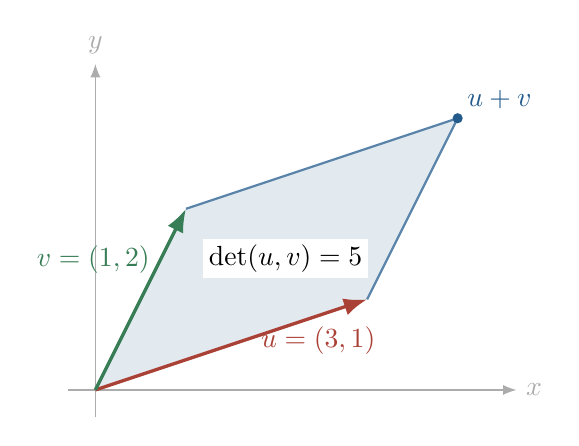
\begin{tikzpicture}[>=Latex,scale=1.15]
 \coordinate (O) at (0,0);
 \coordinate (U) at (3,1);
 \coordinate (V) at (1,2);
 \coordinate (UV) at (4,3);
 \fill[manifoldblue!13] (O)--(U)--(UV)--(V)--cycle;
 \draw[->,gray!65] (-0.3,0)--(4.65,0) node[right] {$x$};
 \draw[->,gray!65] (0,-0.3)--(0,3.6) node[above] {$y$};
 \draw[thick,manifoldblue!75] (U)--(UV)--(V);
 \draw[->,very thick,manifoldred] (O)--(U)
   node[pos=0.82,below] {$u=(3,1)$};
 \draw[->,very thick,manifoldgreen] (O)--(V)
   node[pos=0.72,left] {$v=(1,2)$};
 \fill[manifoldblue] (UV) circle (1.6pt) node[above right] {$u+v$};
 \node[fill=white,inner sep=2pt] at (2.1,1.45)
   {$\det(u,v)=5$};
\end{tikzpicture}
\caption{Iloczyn zewnętrzny w $\R^2$ koduje pole i orientację
równoległoboku. Zmiana kolejności wektorów zmienia znak.}
\label{fig:wedge-pole}
\end{figure}

\begin{twierdzenie}[Minory jako macierz $\Lambda^k A$]
\label{thm:minory-lambda}
Niech $A\colon\mathbb K^n\to\mathbb K^m$ ma macierz
$(a_{ij})$. W bazach uporządkowanych z
Twierdzenia~\ref{thm:wedge-baza} współczynnik macierzy
$\Lambda^k A$ w wierszu $I=(i_1<\cdots<i_k)$ i kolumnie
$J=(j_1<\cdots<j_k)$ jest wyznacznikiem podmacierzy
$A_{I,J}=(a_{i_a,j_b})_{a,b=1}^k$.
\end{twierdzenie}
\begin{proof}
Rozwijamy
$Ae_{j_1}\wedge\cdots\wedge Ae_{j_k}$ według
$Ae_{j_b}=\sum_i a_{i,j_b}e_i$. Przy bazowym
$e_{i_1}\wedge\cdots\wedge e_{i_k}$ pojawiają się tylko
składniki, których $k$ indeksów stanowi permutację $I$.
Po ustawieniu ich w kolejności rosnącej dostajemy
\[
 \sum_{\sigma\in S_k}\operatorname{sgn}(\sigma)
 \prod_{b=1}^k a_{i_{\sigma(b)},j_b}
 =\det A_{I,J}
\]
na mocy wzoru~\eqref{eq:det-leibniz} dla macierzy $k\times k$.
Nie występują żadne inne składniki przy wskazanym
wektorze bazowym, więc to jest szukany współczynnik.
\end{proof}

\begin{wniosek}[Wzór Cauchy'ego--Bineta]
\label{cor:cauchy-binet}
Dla macierzy $A$ o wymiarach $m\times n$ i $B$ o wymiarach
$n\times p$, oraz rosnących indeksów $I\subseteq\{1,\ldots,m\}$,
$J\subseteq\{1,\ldots,p\}$ długości $k$, gdzie $0\leq k\leq\min(m,p)$,
zachodzi
\begin{equation}\label{eq:cauchy-binet}
 \det\bigl((AB)_{I,J}\bigr)
 =\sum_{\substack{K\subseteq\{1,\ldots,n\}\\ |K|=k}}
 \det A_{I,K}\,\det B_{K,J}.
\end{equation}
\end{wniosek}
\begin{proof}
Z Twierdzenia~\ref{thm:potega-zewn-operatora} mamy
$\Lambda^k(AB)=(\Lambda^k A)(\Lambda^k B)$.
Twierdzenie~\ref{thm:minory-lambda} mówi, że macierze
trzech występujących tu operatorów mają za współczynniki
odpowiednie minory. Współczynnik iloczynu macierzy w
wierszu $I$ i kolumnie $J$ to suma po wszystkich
$k$-elementowych indeksach pośrednich $K$; jest ona
dokładnie prawą stroną~\eqref{eq:cauchy-binet}.
Dla $k=0$ obie strony są równe $1$. Gdy $k>n$,
nie ma indeksów $K$ i suma jest zerowa, zgodnie z tym,
że $\Lambda^k(\mathbb K^n)=0$.
\end{proof}

Oznaczamy przez $\operatorname{Alt}^k(V;\mathbb K)$ przestrzeń
alternujących $k$-liniowych funkcji $V^k\to\mathbb K$.
Dla $k=0$ jest to $\mathbb K$.

\begin{twierdzenie}[Kowektory zewnętrzne jako odwzorowania alternujące]
\label{thm:dual-zewnetrzny}
Dla skończenie wymiarowego $V$ istnieje kanoniczny izomorfizm
\[
 \mathcal E_k\colon\Lambda^k(V^*)
 \longrightarrow\operatorname{Alt}^k(V;\mathbb K),
\]
ustalony na iloczynach prostych przez
\begin{equation}\label{eq:wedge-form-det}
 \mathcal E_k(\alpha_1\wedge\cdots\wedge\alpha_k)
 (v_1,\ldots,v_k)
 =\det\bigl(\alpha_a(v_b)\bigr)_{a,b=1}^k.
\end{equation}
W szczególności $\Lambda^k(V^*)\cong(\Lambda^k V)^*$.
Dla kowektorów $\alpha,\beta$ otrzymujemy
\begin{equation}\label{eq:wedge-kowektory}
 \mathcal E_2(\alpha\wedge\beta)(u,v)
 =\alpha(u)\beta(v)-\alpha(v)\beta(u).
\end{equation}
Dla $k=0$ przyjmujemy $\mathcal E_0=\id_{\mathbb K}$ i wyznacznik
pustej macierzy równy $1$. Dla $k>\dim V$ obie strony izomorfizmu
są przestrzeniami zerowymi.
\end{twierdzenie}
\begin{proof}
Wyznacznik w~\eqref{eq:wedge-form-det} jest wieloliniowy
i alternujący w wierszach, a zatem w $\alpha_a$;
Twierdzenie~\ref{thm:wedge-multilinear}, zastosowane do $V^*$,
zapewnia dobrze określone odwzorowanie liniowe $\mathcal E_k$.
Jest ono alternujące w argumentach $v_b$, bo zamiana dwóch
kolumn wyznacznika zmienia znak, i wieloliniowe w tych
argumentach. Jeśli $e^1,\ldots,e^n$ jest bazą dualną,
to wartość $\mathcal E_k(e^{i_1}\wedge\cdots\wedge e^{i_k})$
na $(e_{j_1},\ldots,e_{j_k})$, dla indeksów rosnących,
wynosi $\delta_{I,J}$. Wektory bazowe w
$\Lambda^k(V^*)$ przechodzą więc na bazę dualną do
wektorów bazowych $\Lambda^k V$: daje to izomorfizm
$\Lambda^k(V^*)\cong(\Lambda^k V)^*$.
Każde odwzorowanie alternujące $V^k\to\mathbb K$ wyznacza
funkcjonał na $\Lambda^k V$ przez
Twierdzenie~\ref{thm:wedge-multilinear}, więc powyższy
izomorfizm obejmuje dokładnie wszystkie takie odwzorowania.
Przy $k=2$ wzór wyznacznika $2\times2$ daje
równość~\eqref{eq:wedge-kowektory}.
\end{proof}

\begin{uwaga}[Dwie zgodne normalizacje]
Utożsamienie $j_2$ z Twierdzenia~\ref{thm:wedge-alt} wysyła
$\alpha\wedge\beta$ na
$\tfrac12(\alpha\otimes\beta-\beta\otimes\alpha)$.
Natomiast $\mathcal E_2$ wysyła go na \emph{dwukrotność}
tego antysymetrycznego odwzorowania dwuliniowego: wzór
\eqref{eq:wedge-kowektory} nie zawiera czynnika $1/2$.
Ogólnie, po odczytaniu tensorów kowariantnych jako funkcji wieloliniowych,
zachodzi $\mathcal E_k=k!\,j_k$: suma w wyznaczniku ma te same
składniki ze znakami co antysymetryzacja, lecz bez dzielenia przez $k!$.
Po utożsamieniu elementów $\Lambda^k(V^*)$ z
odwzorowaniami alternującymi za pomocą $\mathcal E_k$, iloczyn
$\omega\wedge\eta$ stopni $k$ i $\ell$ jest dany przez
\begin{equation}\label{eq:wedge-alt-forms}
 (\omega\wedge\eta)(v_1,\ldots,v_{k+\ell})
 =\frac1{k!\ell!}\sum_{\sigma\in S_{k+\ell}}
 \operatorname{sgn}(\sigma)
 \omega(v_{\sigma(1)},\ldots,v_{\sigma(k)})
 \eta(v_{\sigma(k+1)},\ldots,v_{\sigma(k+\ell)}).
\end{equation}
Dla iloczynów kowektorów prostych jest to rozwinięcie
wyznacznika względem pierwszych $k$ wierszy: każdemu
wyborowi $k$ kolumn odpowiada $k!\ell!$ permutacji
wewnątrz dwóch bloków. Ponieważ takie iloczyny rozpinają
przestrzenie zewnętrzne, wzór zachodzi zawsze.
Równoważnie współczynnik przed
$\operatorname{Alt}_{k+\ell}(\omega\otimes\eta)$ jest równy
$(k+\ell)!/(k!\ell!)$, gdy $\omega,\eta$ są już funkcjami
alternującymi. Wynika to bezpośrednio z
$\mathcal E_m=m!j_m$ i wzoru na mnożenie dla $j_m$.
To wyjaśnia, dlaczego wzór w modelu tensorów antysymetrycznych
i wzór dla form mają różne współczynniki, mimo że opisują tę samą algebrę.
\end{uwaga}

\section{Tensory w punkcie rozmaitości}
\label{sec:tensory-rozmaitosc}

Dla gładkiej rozmaitości $M$ i $p\in M$ bierzemy teraz
$V=T_pM$ jako rzeczywistą przestrzeń liniową, a
$V^*=T_p^*M$ z Sekcji~\ref{sec:przestrzen-styczna}
i~\ref{sec:przestrzen-kostyczna}. Tensor typu $(r,s)$
\emph{w punkcie} $p$ jest elementem $T^r_s(T_pM)$;
to pojedynczy obiekt w jednym włóknie.

\begin{stwierdzenie}[Iloczyn tensorowy wiązek]
\label{prop:tensor-wiazek}
Niech $E,F\to M$ będą wiązkami wektorowymi rzędów
odpowiednio $a,b$. Przestrzenie $(E\otimes F)_p:=E_p\otimes F_p$
tworzą wiązkę wektorową rzędu $ab$ nad $M$. Jeśli
$g_{ji}$ i $h_{ji}$ są macierzami przejścia wiązek
$E$ i $F$, to macierzami przejścia $E\otimes F$
są $g_{ji}\otimes h_{ji}$.
\end{stwierdzenie}

\begin{proof}
Na obszarze, gdzie $E$ i $F$ mają bazy lokalne
$e_1,\ldots,e_a$ oraz $f_1,\ldots,f_b$, ich $ab$
iloczynów $e_u\otimes f_v$ stanowi bazę każdego włókna
$E_p\otimes F_p$ na mocy twierdzenia o bazie iloczynu
tensorowego. Gdy zmienimy obie bazy, wzór na współczynniki
iloczynu prostego pokazuje, że nowe współczynniki otrzymujemy
przez przemnożenie starych macierzą $g_{ji}\otimes h_{ji}$;
jej elementy są iloczynami gładkich funkcji. Na przecięciu
trzech obszarów własność złożenia z
Twierdzenia~\ref{thm:tensor-operatorow} daje
\[
 (g_{kj}\otimes h_{kj})(g_{ji}\otimes h_{ji})
   =(g_{kj}g_{ji})\otimes(h_{kj}h_{ji})
   =g_{ki}\otimes h_{ki}.
\]
Jest to warunek sklejania; macierze są odwracalne,
bo ich odwrotnościami są $g_{ji}^{-1}\otimes h_{ji}^{-1}$.
Konstrukcja wiązki z takich danych, podana w
Sekcji~\ref{sec:wiazki-wektorowe}, kończy dowód.
\end{proof}

\begin{definicja}[Pole tensorowe]
\index{pole tensorowe@Pole tensorowe}
\label{def:pole-tensorowe}
\emph{Pole tensorowe} typu $(r,s)$ przypisuje każdemu
$p\in M$ tensor $T_p\in T^r_s(T_pM)$ w sposób gładki.
Dokładnie: jest gładkim przekrojem wiązki
\begin{equation}\label{eq:wiazka-tensorowa}
 T^r_s M:=(TM)^{\otimes r}\otimes(T^*M)^{\otimes s}
 \longrightarrow M.
\end{equation}
Przy wykładniku $0$ rozumiemy czynnik jako wiązkę
trywialną $M\times\R$.
\end{definicja}

W lokalnej mapie $x^1,\ldots,x^n$ bazami włókien są
$\partial_i:=\partial/\partial x^i$ oraz dualne
$\dd x^j$, określone przez $\dd x^j(\partial_i)=\delta_i^j$.
Pole ma zatem postać
\begin{equation}\label{eq:pole-tensorowe-lokalnie}
 T=\sum_{\substack{i_1,\ldots,i_r\\j_1,\ldots,j_s}}
 T^{i_1\cdots i_r}{}_{j_1\cdots j_s}(x)
 \partial_{i_1}\otimes\cdots\otimes\partial_{i_r}
 \otimes\dd x^{j_1}\otimes\cdots\otimes\dd x^{j_s}.
\end{equation}
Warunek gładkości oznacza dokładnie, że wszystkie funkcje
$T^{i_1\cdots i_r}{}_{j_1\cdots j_s}(x)$ są gładkie.
W innej mapie bazowe wektory i kowektory się zmieniają;
przepisanie tej samej wartości $T_p$ w nowych bazach
narzuca współczynnikom prawa transformacji, które teraz rozpiszemy.
Niech $x$ i $y$ będą dwiema mapami wokół $p$, a
\[
 A^a{}_i=\frac{\partial y^a}{\partial x^i}(p),\qquad
 B^j{}_b=\frac{\partial x^j}{\partial y^b}(p),\qquad B=A^{-1}.
\]
Reguła łańcucha i dualność dają
\[
 \partial_{x^i}=\sum_a A^a{}_i\partial_{y^a},\qquad
 \dd x^j=\sum_b B^j{}_b\dd y^b.
\]
Podstawiając te równości w każdy czynnik
\eqref{eq:pole-tensorowe-lokalnie}, otrzymujemy
\begin{equation}\label{eq:tensor-zmiana-wspolrzednych}
 (T_y)^{a_1\cdots a_r}{}_{b_1\cdots b_s}
 =\sum_{I,J}
 \left(\prod_{\mu=1}^r A^{a_\mu}{}_{i_\mu}\right)
 \left(\prod_{\nu=1}^s B^{j_\nu}{}_{b_\nu}\right)
 (T_x)^{i_1\cdots i_r}{}_{j_1\cdots j_s}.
\end{equation}
Wszystkie wartości odnoszą się do tego samego punktu $p$;
zmienia się jedynie jego opis i baza. Każdy górny indeks wnosi
macierz Jacobiego $A$, a każdy dolny jej odwrotność $B$.
Odwracając zamianę map, odzyskujemy stare współczynniki.
Ponieważ $A,B$ są gładkie, gładkość współczynników w jednej
mapie pociąga ją w każdej innej.

Wiązka~\eqref{eq:wiazka-tensorowa} powstaje
przez wielokrotne zastosowanie
Stwierdzenia~\ref{prop:tensor-wiazek} do $TM$ i $T^*M$.

Typ $(0,0)$ to zwykła funkcja gładka, typ $(1,0)$ to
pole wektorowe z Rozdziału~\ref{ch:pola}, a typ $(0,2)$
to gładko zmieniająca się rodzina form dwuliniowych
na przestrzeniach stycznych. Iloczyn tensorowy i kontrakcja
działają \emph{punkt po punkcie}. Pozostawiają pola gładkie,
bo w mapach ich współczynniki są sumami iloczynów
gładkich funkcji współczynnikowych.

\begin{przyklad}[Tensor identycznościowy]
Operator $\id_{T_pM}$ z~\eqref{eq:endo-tensor} odpowiada
w dowolnej bazie $e_i$ tensorowi
\[
 \mathsf I_p=\sum_i e_i\otimes e^i\in T^1_1(T_pM).
\]
Jego zapis w mapie to $\sum_i\partial_i\otimes\dd x^i$.
Nie zależy od mapy: po przyłożeniu do dowolnego $v$
odzyskujemy $\sum_i e^i(v)e_i=v$, a izomorfizm
$T^1_1(T_pM)\cong\operatorname{End}(T_pM)$ jest
iniektywny. Tensor $\mathsf I$ jest zatem globalnym
gładkim polem tensorowym, mimo że zapisaliśmy go lokalnie.
\end{przyklad}

\begin{przyklad}[Tensor jako iloczyn skalarny]
Na $\R^2$ pole
$g=\dd x\otimes\dd x+\dd y\otimes\dd y$
przypisuje każdemu punktowi ten sam iloczyn skalarny.
Dla $u=a\partial_x+b\partial_y$ i
$v=c\partial_x+d\partial_y$ mamy
$g(u,v)=ac+bd$. Oznacza to, że tensor typu $(0,2)$
można czytać jako przepis przyjmujący \emph{dwa}
wektory styczne w jednym punkcie i zwracający liczbę.
Sama lista jego współczynników zmieni się przy zamianie
współrzędnych, ale wartość $g(u,v)$ pozostanie ta sama.
Na jednowymiarowym przykładzie widać konkretny czynnik:
dla $x>0$ i $y=x^2$ tensor $\dd x\otimes\dd x$ ma zapis
$\frac1{4y}\dd y\otimes\dd y$, bo
$\dd x=\frac1{2\sqrt y}\dd y$. Zmiana współrzędnych nie
pozwala więc po prostu zastąpić symbolu $x$ symbolem $y$
przy pozostawieniu tych samych współczynników.
\end{przyklad}

Podobnie $\Lambda^k(T_pM)$ ma wymiar $\binom nk$.
W przypadku różniczki $\dd F_p\colon T_pM\to T_{F(p)}N$
między rozmaitościami tego samego wymiaru,
$\Lambda^n(\dd F_p)$ działa między ich jednowymiarowymi
potęgami zewnętrznymi. Jest niezerowe dokładnie wtedy,
gdy $\dd F_p$ jest izomorfizmem: wynika to z dowodu
Twierdzenia~\ref{thm:det-wlasnosci}, zastosowanego do baz
w dwóch różnych przestrzeniach. W mapach odpowiada temu
warunek niezerowego wyznacznika macierzy Jacobiego.
W odróżnieniu od endomorfizmu jednej przestrzeni, dla mapy
$T_pM\to T_{F(p)}N$ nie otrzymujemy jednak kanonicznego skalara
„wyznacznik” bez wyboru baz lub elementów objętości w obu włóknach.
Kanoniczne jest odwzorowanie $\Lambda^n(\dd F_p)$ między
dwiema prostymi; jego macierz liczbową określają wybrane mapy.

\begin{uwaga}[Cztery sposoby widzenia tej samej konstrukcji]
Iloczyn tensorowy powstaje z dwuliniowości
(Definicja~\ref{def:tensor-universal}); algebra tensorowa
gromadzi wszystkie stopnie i mnoży przez konkatenację
(Definicja~\ref{def:algebra-tensorowa}). Symetryzator
$\operatorname{Sym}_k$ wybiera część niezmienniczą względem
permutacji, zaś $\operatorname{Alt}_k$ część zmieniającą znak.
Algebra zewnętrzna jest ilorazem, w którym kwadrat każdego
wektora znika (Definicja~\ref{def:algebra-zewnetrzna}).
Twierdzenie~\ref{thm:wedge-alt} mówi dokładnie, jak przejść
od tego ilorazu do tensorów antysymetrycznych.
\end{uwaga}

\section{Różniczkowanie pól tensorowych: pochodna Liego}
\label{sec:lie-tensory}

Pole tensorowe ma wartości w różnych przestrzeniach nad
różnymi punktami. Dlatego wyrażenie ,,odejmij $T_q-T_p$''
nie ma sensu, dopóki nie wskażemy sposobu przeniesienia
obu tensorów do jednego włókna. W Sekcji~\ref{sec:liego}
przepływ pola $X$ zrobił to dla pól wektorowych;
ta sama konstrukcja działa na każdym typie tensora.

Samo różniczkowanie współczynników w mapie nie rozwiązuje
problemu: ich pochodne zmieniają się przy zmianie współrzędnych.
Na przykład na $(0,\infty)$ wektor $Y=\partial_x$ ma w
mapie $x$ stały współczynnik $Y^x=1$, więc
$\partial_xY^x=0$. Po podstawieniu $y=x^2$ mamy
$Y=2\sqrt y\,\partial_y$ i
$\partial_yY^y=1/\sqrt y\ne0$.
Różnica pochodzi od zmiany samej bazy $\partial_y$.
Pochodna Liego uwzględnia również tę zmianę.

\begin{definicja}[Cofnięcie pola tensorowego]
\index{cofniecie pola tensorowego@Cofnięcie pola tensorowego}
\label{def:cofniecie-tensora}
Niech $F\colon U\to V$ będzie dyfeomorfizmem między
otwartymi podzbiorami $M$. Dla pola wektorowego $Y$ i
pola kowektorowego $\alpha$ na $V$ definiujemy w $p\in U$
\begin{align*}
 (F^*Y)_p&:=(\dd F_p)^{-1}Y_{F(p)}\in T_pM,\\
 (F^*\alpha)_p(v)&:=\alpha_{F(p)}(\dd F_pv),
 \qquad v\in T_pM.
\end{align*}
Dla funkcji kładziemy $F^*f=f\circ F$.
Na tensorach prostych cofamy każdy czynnik osobno,
np.\ $F^*(Y\otimes\alpha)=F^*Y\otimes F^*\alpha$,
i przedłużamy liniowo na sumy w każdym włóknie. Do gładkości
wystarczy lokalne rozwinięcie w bazie tensorowej; nie zakładamy
istnienia jednej globalnej bazy ani globalnego rozkładu na tensory proste.
Dostajemy pole
tego samego typu na $U$. W szczególności
$F^*(fT)=(f\circ F)F^*T$, a nie $fF^*T$.
Współczynniki są gładkie: różniczka i jej macierz odwrotna
zależą gładko od punktu, a działania tensorowe są wieloliniowe.
\end{definicja}

Przy cofaniu wektora używamy odwrotnej różniczki,
a przy cofaniu kowektora różniczki bez odwracania:
obie wartości muszą ostatecznie należeć do włókna nad $p$.
Wzór dla tensorów prostych jest dobrze określony na
iloczynach tensorowych, ponieważ każda z operacji na
czynnikach jest liniowa. W szczególności cofnięcie zachowuje
iloczyn tensorowy i kontrakcję. To drugie można sprawdzić
na jednej parze:
\[
 (F^*\alpha)_p\bigl((F^*Y)_p\bigr)
 =\alpha_{F(p)}\bigl(\dd F_p(\dd F_p)^{-1}Y_{F(p)}\bigr)
 =\alpha_{F(p)}(Y_{F(p)}).
\]
Obie strony są cofnięciem funkcji $p\mapsto\alpha_p(Y_p)$;
z liniowości wynikają analogiczne równości dla innych tensorów.

\begin{definicja}[Pochodna Liego dowolnego pola tensorowego]
\index{pochodna liego dowolnego pola tensorowego@Pochodna Liego dowolnego pola tensorowego}
\label{def:lie-tensor}
Niech $\Phi_t=\Phi_t^X$ oznacza lokalny przepływ pola $X$.
Dla pola tensorowego $T$ dowolnego typu kładziemy
\begin{equation}\label{eq:lie-tensor-def}
 (\Lie_XT)_p
 :=\left.\frac{\dd}{\dd t}\right|_{t=0}
 (\Phi_t^*T)_p.
\end{equation}
Każdy tensor $(\Phi_t^*T)_p$ należy do tej samej
przestrzeni $T^r_s(T_pM)$, zatem pochodna jest
zwykłą pochodną krzywej w przestrzeni liniowej. Jest to gładkie
pole tensorowe: w każdej mapie współczynniki cofnięcia są gładkie
łącznie w $(t,p)$, więc ich pochodne po $t$ w zerze są gładkie w $p$.
\end{definicja}

W stopniu $(0,0)$ wzór~\eqref{eq:lie-tensor-def} daje
$\Lie_Xf=X(f)$, ponieważ $\Phi_t^*f=f\circ\Phi_t$.
Dla typu $(1,0)$ odzyskujemy dokładnie
$\Lie_XY=[X,Y]$ z Twierdzenia~\ref{thm:lie-nawias}.
Dowód tamtego twierdzenia wyjaśnia szczegółowo znak:
przenosimy $Y_{\Phi_t(p)}$ z powrotem różniczką
przepływu $\Phi_{-t}$.

\begin{twierdzenie}[Reguła Leibniza i zgodność z kontrakcją]
\label{thm:lie-tensor-reguly}
Dla pól tensorowych $S,T$, funkcji $f$, pola wektorowego
$Y$ i pola kowektorowego $\alpha$ mamy
\begin{align}
 \Lie_X(S\otimes T)
 &= (\Lie_XS)\otimes T+S\otimes(\Lie_XT),
 \label{eq:lie-tensor-leibniz}\\
 \Lie_X(fT)&=X(f)T+f\Lie_XT,
 \label{eq:lie-tensor-funkcja}\\
 (\Lie_X\alpha)(Y)
 &=X\bigl(\alpha(Y)\bigr)-\alpha([X,Y]),
 \label{eq:lie-kowektor}\\
 \Lie_X(C(S))&=C(\Lie_XS),
 \label{eq:lie-kontrakcja}
\end{align}
gdzie w ostatnim wzorze $C$ jest dowolną kontrakcją
jednego indeksu wektorowego z jednym kowektorowym.
\end{twierdzenie}
\begin{proof}
Ustalmy punkt $p$. Cofnięcie zachowuje iloczyn tensorowy:
$\Phi_t^*(S\otimes T)=\Phi_t^*S\otimes\Phi_t^*T$.
Obie krzywe tensorów po prawej stronie leżą w stałych
przestrzeniach nad $p$; różniczkując ich iloczyn
dwuliniowy w $t=0$ dostajemy
\eqref{eq:lie-tensor-leibniz}. Traktując $f$ jako tensor
typu $(0,0)$, otrzymujemy
\eqref{eq:lie-tensor-funkcja} z $\Lie_Xf=X(f)$.

Dla kowektora i wektora równanie o zachowaniu ewaluacji,
wykazane tuż przed definicją, przyjmuje postać
\[
 \Phi_t^*\bigl(\alpha(Y)\bigr)
 =(\Phi_t^*\alpha)(\Phi_t^*Y).
\]
Lewa strona po zróżniczkowaniu w zerze wynosi
$X(\alpha(Y))$. Prawa, przez zwykłą regułę
różniczkowania wartości kowektora na wektorze,
wynosi $(\Lie_X\alpha)(Y)+\alpha(\Lie_XY)$.
Z~$\Lie_XY=[X,Y]$ otrzymujemy
\eqref{eq:lie-kowektor}.

Wreszcie, cofnięcie i kontrakcja spełniają
$\Phi_t^*C(S)=C(\Phi_t^*S)$, co dla pojedynczej
pary sprawdziliśmy powyżej. Kontrakcja jest liniowym
odwzorowaniem między przestrzeniami tensorów w $p$, więc
można ją przenieść przez pochodną po $t$.
To daje~\eqref{eq:lie-kontrakcja}.
\end{proof}

\begin{twierdzenie}[Wzór we współrzędnych]
\label{thm:lie-tensor-wspolrzedne}
Niech $X=\sum_{a=1}^nX^a\partial_a$ i niech $T$ ma
współczynniki $T^I{}_J$ z~\eqref{eq:pole-tensorowe-lokalnie},
gdzie $I=(i_1,\ldots,i_r)$ i $J=(j_1,\ldots,j_s)$.
Symbol $I_{\mu\leftarrow a}$ oznacza zastąpienie w $I$
indeksu $i_\mu$ przez $a$, a $J_{\nu\leftarrow a}$
oznacza to samo w $J$. Wtedy
\begin{equation}\label{eq:lie-tensor-komponenty}
\begin{aligned}
 (\Lie_XT)^I{}_J
 &=\sum_{a=1}^nX^a\partial_a T^I{}_J
 -\sum_{\mu=1}^r\sum_{a=1}^n
   (\partial_aX^{i_\mu})T^{I_{\mu\leftarrow a}}{}_J\\
 &\quad+\sum_{\nu=1}^s\sum_{a=1}^n
   (\partial_{j_\nu}X^a)T^I{}_{J_{\nu\leftarrow a}}.
\end{aligned}
\end{equation}
Pierwszy wyraz różniczkuje funkcje współczynnikowe,
każdy indeks wektorowy wnosi wyraz z minusem,
a każdy indeks kowektorowy wyraz z plusem.
Na przykład dla pola operatorów $S\in\Gamma(T^1_1M)$
wzór ten ma łatwą do odczytania postać
\[
 (\Lie_XS)^i{}_j
 =\sum_a X^a\partial_aS^i{}_j
  -\sum_a S^a{}_j\partial_aX^i
  +\sum_a S^i{}_a\partial_jX^a.
\]
\end{twierdzenie}
\begin{proof}
Z~\eqref{eq:nawias-wspolrzedne}, zastosowanego do
$Y=\partial_i$, wynika
\[
 \Lie_X\partial_i=[X,\partial_i]
 =-\sum_a(\partial_iX^a)\partial_a,
\]
ponieważ współczynniki pola $\partial_i$ są stałe.
Z kolei $\dd x^j(\partial_i)=\delta_i^j$ jest funkcją
stałą. Wstawiając $Y=\partial_i$ i $\alpha=\dd x^j$
do~\eqref{eq:lie-kowektor}, dostajemy
\[
 (\Lie_X\dd x^j)(\partial_i)
 =X(\delta_i^j)-\dd x^j([X,\partial_i])
 =\partial_iX^j.
\]
Wektory $\partial_i$ tworzą bazę, zatem
$\Lie_X\dd x^j=\sum_i(\partial_iX^j)\dd x^i$.
Teraz rozwińmy $T$ według~\eqref{eq:pole-tensorowe-lokalnie}
i stosujmy~\eqref{eq:lie-tensor-leibniz} kolejno
do funkcji współczynnikowej oraz do każdego czynnika.
Różniczkowanie funkcji daje pierwszy wyraz
\eqref{eq:lie-tensor-komponenty}. Dla ustalonego miejsca
wektorowego $\mu$ współczynnik przy bazowym
$\partial_{i_\mu}$ po zróżniczkowaniu wcześniejszego
czynnika $\partial_a$ wynosi
$-\sum_a(\partial_aX^{i_\mu})T^{I_{\mu\leftarrow a}}{}_J$;
sumowanie po $\mu$ daje drugi wyraz wzoru.
Dla ustalonego miejsca kowektorowego $\nu$ wcześniejszy
czynnik $\dd x^a$ wnosi do współczynnika przy
$\dd x^{j_\nu}$ sumę
$\sum_a(\partial_{j_\nu}X^a)T^I{}_{J_{\nu\leftarrow a}}$;
po zsumowaniu po $\nu$ otrzymujemy trzeci wyraz.
Ponieważ tensory bazowe są liniowo niezależne,
ich współczynniki są dokładnie podanymi wyrażeniami.
\end{proof}

\begin{przyklad}[Sprawdzenie znaków na przepływie]
Na $\R^2$ weźmy $X=x\partial_x$. Jego przepływ to
$\Phi_t(x,y)=(e^tx,y)$, więc
\[
 \Phi_t^*\partial_x=e^{-t}\partial_x,
 \qquad \Phi_t^*\dd x=e^t\dd x.
\]
Po zróżniczkowaniu w zerze otrzymujemy
$\Lie_X\partial_x=-\partial_x=[X,\partial_x]$
oraz $\Lie_X\dd x=\dd x$. Pierwszy znak jest ujemny,
bo cofamy wektor różniczką odwrotnego przepływu;
drugi dodatni, bo kowektor działa na różniczce przepływu.
Wyniki są zgodne z tym, że $\dd x(\partial_x)=1$
pozostaje funkcją stałą: $1+(-1)=0$ w regule
Leibniza dla ewaluacji.
\end{przyklad}

\begin{przyklad}[Jak zmienia się tensor metryczny]
Dla $g=\dd x\otimes\dd x+\dd y\otimes\dd y$ i
$X=x\partial_x$ mamy
\[
 \Phi_t^*g=e^{2t}\dd x\otimes\dd x
             +\dd y\otimes\dd y,\qquad
 \Lie_Xg=2\dd x\otimes\dd x.
\]
Przepływ rozciąga kierunek $x$; gdy tensor mierzy
iloczyny skalarne dwóch wektorów, pojawia się czynnik
$e^t$ dla każdego z dwóch kowektorowych miejsc.
\end{przyklad}

\begin{uwaga}[Jaką pochodną zdefiniowaliśmy?]
Pochodna Liego porównuje tensory za pomocą przepływu
\emph{konkretnego} pola $X$. Jej wzór wymaga tylko struktury
gładkiej i pola $X$. Jeśli chcielibyśmy porównywać tensory
wzdłuż dowolnej krzywej bez wskazanego przepływu,
potrzebowalibyśmy dodatkowej reguły przenoszenia między
przestrzeniami stycznymi, nazywanej \emph{koneksją} (połączeniem).
Na przykład $\Lie_{x\partial_x}\partial_x=-\partial_x$
chociaż współczynniki pola $\partial_x$ są stałe:
wynik uwzględnia ruch bazy pod przepływem.
\end{uwaga}

\par\smallskip
{\footnotesize\noindent\emph{Dalsza lektura:}
\href{https://math.stanford.edu/~conrad/diffgeomPage/handouts/tensor.pdf}
{B. Conrad, \emph{Tensor algebras, tensor pairings, and duality}},
notatki do Math 396, s. 1--13: własności uniwersalne i dualność;
\href{https://doi.org/10.1007/978-1-4419-9982-5}
{J. M. Lee, \emph{Introduction to Smooth Manifolds}, wyd. 2},
rozdziały 12 i 14: pola tensorowe, formy alternujące
i pochodne Liego.\par}
\clearpage

\chapter{Grassmanniany, algebra Clifforda i spinory}
\label{ch:grass-spin}
\index{grupa spin@Grupa Spin}

W Rozdziale~\ref{ch:algebra-tensorowa} skonstruowaliśmy iloczyn
zewnętrzny i wiązki tensorowe. Teraz zadamy trzy kolejne pytania:
jak opisać \emph{przestrzeń wszystkich podprzestrzeni} danego wymiaru,
jak zmienić algebrę zewnętrzną, aby uwzględniała iloczyn skalarny,
i dlaczego obrót o $2\pi$ może zmieniać znak spinora.
Odpowiedzi prowadzą kolejno do grassmannianów, algebr Clifforda
i grup Spin. Przykłady w wymiarach $2$ i $3$ pozwolą nam
sprawdzać każdą konwencję znaku na konkretnych macierzach.

\section{Grassmannian jako przestrzeń podprzestrzeni}
\label{sec:grass-atlas}

Przez $\mathbb K$ oznaczamy w tej sekcji $\R$ albo $\C$.
Jeśli $0\leq k\leq n$, \emph{grassmannian}
$\operatorname{Gr}_k(\mathbb K^n)$ to zbiór wszystkich
$k$-wymiarowych podprzestrzeni liniowych $\mathbb K^n$.
Jego \emph{punktem} jest cała podprzestrzeń $L$,
a nie wektor w $L$. Na przykład
$\operatorname{Gr}_1(\R^n)=\mathbb{RP}^{n-1}$
z Przykładu~\ref{prz:RPn}, a
$\operatorname{Gr}_1(\C^n)=\mathbb{CP}^{n-1}$.
Dla $k=0$ i $k=n$ grassmannian jest jednym punktem.
Dla dowolnej $n$-wymiarowej przestrzeni $V$ nad $\mathbb K$
piszemy analogicznie $\operatorname{Gr}_k(V)$; wybór bazy
identyfikuje go z powyższym modelem, lecz konstrukcje nie zależą od tej bazy.

\begin{twierdzenie}[Mapy wykresowe grassmannianu]
\label{thm:grass-atlas}
Niech $\mathbb K^n=P\oplus Q$, gdzie $\dim_{\mathbb K}P=k$.
Zbiór
\[
 U_P=\{L\in\operatorname{Gr}_k(\mathbb K^n):
           \pi_P|_L:L\longrightarrow P\text{ jest izomorfizmem}\}
\]
można jednoznacznie opisać odwzorowaniami liniowymi
$A:P\to Q$: punktowi $A$ odpowiada jego
\emph{wykres} $\Gamma(A)=\{u+Au:u\in P\}$.
Mapy $\Gamma(A)\mapsto A$ tworzą gładki atlas
grassmannianu. Jego wymiar nad $\mathbb K$ wynosi
$k(n-k)$. W przypadku zespolonym atlas jest holomorficzny,
a rzeczywisty wymiar wynosi $2k(n-k)$.
Oznaczenie $U_P$ zależy również od wybranego dopełnienia $Q$;
pomijamy je w indeksie tylko dla skrócenia zapisu.
\end{twierdzenie}
\begin{proof}
Jeśli $L=\Gamma(A)$, to $\pi_P(u+Au)=u$, więc
$\pi_P|_L$ jest izomorfizmem. W drugą stronę, dla
$L\in U_P$ określmy
\[
 A_L:=\pi_Q|_L\circ(\pi_P|_L)^{-1}:P\longrightarrow Q.
\]
Każdy $v\in L$ ma postać $u+\pi_Qv=u+A_Lu$
dla $u=\pi_Pv$. Stąd $L=\Gamma(A_L)$; dowiedliśmy
zarówno istnienia, jak i jednoznaczności parametru.

Sprawdźmy przejścia między mapami, a nie tylko ich
liczbę. Niech $\mathbb K^n=P'\oplus Q'$ będzie drugim
rozkładem. Dla $A:P\to Q$ połóżmy
$T_A:P\to\mathbb K^n$, $T_A(u)=u+Au$.
Wykres $\Gamma(A)$ należy do $U_{P'}$ dokładnie wtedy,
gdy $D_A:=\pi_{P'}T_A:P\to P'$ jest odwracalny.
Po wybraniu baz $P,P'$ wyznacznik macierzy $D_A$ zależy
wielomianowo od współczynników $A$;
warunek $\det D_A\ne0$ jest więc otwarty. W nowej mapie
parametr ma postać
\begin{equation}\label{eq:grass-przejscie}
 A'=\pi_{Q'}T_A\circ(\pi_{P'}T_A)^{-1}:P'\longrightarrow Q'.
\end{equation}
Odwracanie macierzy jest gładkie na zbiorze macierzy
odwracalnych, a nad $\C$ jest tam także holomorficzne
(wzór przez dopełnienia algebraiczne i wyznacznik).
Każde $L$ leży w $U_L$, bo dla rozkładu
$\mathbb K^n=L\oplus Q$ otrzymujemy $A_L=0$.
Atlasy pokrywają zatem cały zbiór. Współczynniki
$A\in\operatorname{Hom}_{\mathbb K}(P,Q)$ tworzą
przestrzeń $\mathbb K^{(n-k)k}$, co daje wymiar.

Definiujemy topologię przez atlas: zbiór jest otwarty, gdy
jego obraz w każdej z map wykresowych jest otwarty.
Otwartość dziedzin przejść i ich ciągłość zapewniają, że
same $U_P$ są otwarte, a mapy są homeomorfizmami.
Uzasadnijmy również pozostałe własności topologiczne.
Wybierzmy standardowy iloczyn skalarny, a nad $\C$ hermitowski;
gwiazdka oznacza operator sprzężony. W tym kroku
ograniczmy się do rozkładów ortogonalnych $Q=P^\perp$;
takie mapy wciąż pokrywają cały grassmannian
(dla danego $L$ bierzemy $P=L$).
Wzór~\eqref{eq:grass-przejscie} zapewnia zgodność
z pozostałymi mapami. Każdemu $L$
przypiszmy macierz rzutowania ortogonalnego $\Pi_L$.
Jest ona wyznaczona jednoznacznie przez $L$, a jej
współczynniki w mapie wykresowej są gładkie:
\[
 \Pi_{\Gamma(A)}
  =T_A(T_A^*T_A)^{-1}T_A^*.
\]
Odwrót na $U_P$ jest również ciągły w macierzach
rzutowania, ponieważ dla $L\in U_P$
\[
 A_L=\pi_Q\Pi_L|_P\,(\pi_P\Pi_L|_P)^{-1}.
\]
Ostatnia odwrotność istnieje, gdyż przy ortogonalnym
rzutowaniu $\pi_P$ odwzorowanie $\Pi_L|_P:P\to L$
jest sprzężeniem izomorfizmu
$\pi_P|_L:L\to P$. Nasza topologia zgadza się więc
z topologią podzbioru macierzy rzutowania: $U_P$ jest w tym
modelu zbiorem, gdzie $\pi_P\Pi_L|_P$ jest odwracalne,
a więc zbiorem otwartym. Oba podane wzory są ciągłe na tych mapach.
Zbiór $\Pi^*=\Pi$, $\Pi^2=\Pi$, $\operatorname{tr}\Pi=k$
jest domknięty i ograniczony w skończenie wymiarowej
przestrzeni macierzy, a więc zwarty. Istotnie, samosprzężone
idempotenty mają wartości własne $0,1$, więc norma operatorowa
jest co najwyżej $1$, a ślad jest rangą. Są zatem dokładnie
rzutami na $k$-płaszczyzny. Ten model jest także
Hausdorffa i ma przeliczalną bazę. Atlas definiuje
zatem rozmaitość w sensie Rozdziału~\ref{ch:rozmaitosci}.
\end{proof}

\begin{figure}[!htbp]
\centering
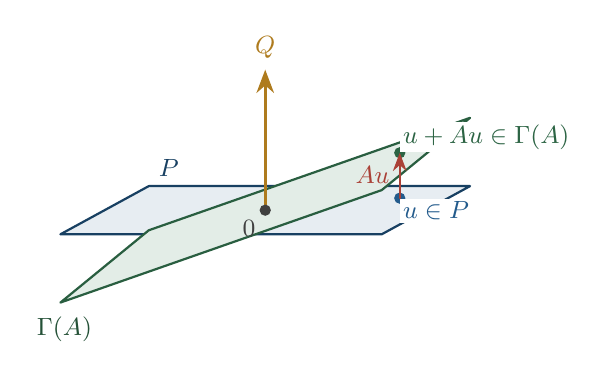
\begin{tikzpicture}[>=Stealth,line cap=round,line join=round,scale=1.02]
 \filldraw[fill=manifoldblue!11,draw=manifoldblue!70!black,thick]
 (-2.55,-.3)--(1.45,-.3)--(2.55,.3)--(-1.45,.3)--cycle;
 \filldraw[fill=manifoldgreen!14,draw=manifoldgreen!75!black,thick]
 (-2.55,-1.15)--(1.45,.25)--(2.55,1.15)--(-1.45,-.25)--cycle;
 \draw[->,manifoldgold!85!black,very thick] (0,0)--(0,1.75)
  node[above,font=\small] {$Q$};
 \fill[black!75] (0,0) circle (2pt) node[below left,font=\small] {$0$};
 \fill[manifoldblue] (1.675,.15) circle (2pt)
  node[below right,fill=white,inner sep=1pt,font=\small] {$u\in P$};
 \fill[manifoldgreen!80!black] (1.675,.715) circle (2pt)
  node[above right,fill=white,inner sep=1pt,font=\small] {$u+Au\in\Gamma(A)$};
 \draw[->,manifoldred,thick] (1.675,.15)--(1.675,.715)
  node[midway,left,font=\small] {$Au$};
 \node[manifoldblue!70!black,font=\small\bfseries] at (-1.2,.52) {$P$};
 \node[manifoldgreen!65!black,font=\small\bfseries] at (-2.5,-1.48) {$\Gamma(A)$};
\end{tikzpicture}
\caption{Mapa wykresowa grassmannianu. Przestrzeń $P$ jest
punktem odniesienia; pobliska płaszczyzna $\Gamma(A)$ powstaje,
gdy nad $u\in P$ odkładamy przemieszczenie $Au\in Q$.}
\label{fig:grass-wykres}
\end{figure}

\begin{przyklad}[Mała mapa, a nie cały grassmannian]
Na $\operatorname{Gr}_1(\R^2)=\mathbb{RP}^1$ ustalmy
$P=\R e_1$ i $Q=\R e_2$. Prosta
$L_a=\operatorname{span}(e_1+ae_2)$ ma współrzędną
$a\in\R$. Brakuje dokładnie jednej prostej, $\R e_2$:
rzutowanie na $P$ jest na niej zerowe. Zatem mapa
wykresowa jest lokalna, podobnie jak mapa stereograficzna
nie pokrywa całej sfery.
\end{przyklad}

\section{Przestrzeń styczna i wiązka tautologiczna}
\label{sec:grass-styczna}

Wektor styczny do grassmannianu opisuje \emph{pierwszy
rząd zmiany podprzestrzeni}. Wektory należące już do
danej podprzestrzeni nie zmieniają jej położenia:
istotna jest część wychodząca poza nią.

\begin{twierdzenie}[Styczne jako odwzorowania do ilorazu]
\label{thm:grass-styczna}
Dla $L\in\operatorname{Gr}_k(V)$ istnieje kanoniczny
izomorfizm
\begin{equation}\label{eq:grass-styczna}
 T_L\operatorname{Gr}_k(V)
  \cong\operatorname{Hom}_{\mathbb K}(L,V/L).
\end{equation}
Nad $\C$ prawa strona jest zespoloną przestrzenią
styczną; jej podłożem rzeczywistym jest rzeczywista
przestrzeń styczna.
\end{twierdzenie}
\begin{proof}
Niech $L(t)$ będzie gładką krzywą podprzestrzeni,
$L(0)=L$. Dla $v\in L$ wybierzmy gładką krzywą
$v(t)\in L(t)$ z $v(0)=v$. Definiujemy
$D_{L'(0)}(v):=[v'(0)]\in V/L$, gdzie nawias oznacza
klasę modulo $L$. Pokażmy niezależność od wyboru
$v(t)$. Różnica dwóch takich krzywych $w(t)\in L(t)$
ma $w(0)=0$. W gładkiej lokalnej bazie $s_i(t)$
zapisuje się $w(t)=\sum_i a_i(t)s_i(t)$ z
$a_i(0)=0$, zatem
$w'(0)=\sum_i a_i'(0)s_i(0)\in L$. Klasa
$[v'(0)]$ nie zmienia się. Zmiana parametryzacji
krzywej nie jest jedyną możliwą zmianą przedstawiciela wektora
stycznego; niezależność od dowolnej krzywej o tym samym wektorze
stycznym sprawdzimy teraz w mapie.

Ustalmy teraz uzupełnienie $V=L\oplus Q$.
W mapie z Twierdzenia~\ref{thm:grass-atlas} mamy
$L(t)=\Gamma(A(t))$ i $A(0)=0$.
Wybieramy $v(t)=v+A(t)v$. Wtedy
\[
 D_{L'(0)}(v)=[A'(0)v]\in V/L.
\]
Tak samo $s_i(t)=e_i+A(t)e_i$ dla bazy $(e_i)$ przestrzeni $L$
daje gładką bazę używaną powyżej. Wzór zależy tylko od $A'(0)$,
czyli współrzędnych wektora stycznego, a nie od dalszego przebiegu krzywej.
Jeśli $D_{L'(0)}=0$, to $A'(0)v\in Q\cap L=0$ dla każdego $v$,
więc $A'(0)=0$ i wektor styczny jest zerowy. To dowodzi iniektywności.
Utożsamienie $Q\cong V/L$ pokazuje, że
$D_{L'(0)}$ jest liniowe w $v$. Każdy
$D\in\operatorname{Hom}(L,V/L)$ można otrzymać:
wybierzmy odpowiadające mu odwzorowanie $A:L\to Q$
i krzywą $L(t)=\Gamma(tA)$. Jej pochodna daje
właśnie $D$. Konstrukcja rozpoczęła się od
krzywej i klas modulo $L$, więc otrzymany
izomorfizm nie zależy od wybranego $Q$.
\end{proof}

\begin{definicja}[Wiązka tautologiczna]
\index{wiazka tautologiczna@Wiązka tautologiczna}
\label{def:grass-taut}
Nad $\operatorname{Gr}_k(V)$ określamy
\emph{wiązkę tautologiczną}
\[
 \gamma^k
 :=\{(L,v)\in\operatorname{Gr}_k(V)\times V:v\in L\}
 \longrightarrow\operatorname{Gr}_k(V),\qquad (L,v)\mapsto L.
\]
Jej włókno w punkcie $L$ jest dosłownie podprzestrzenią
$L\subseteq V$.
\end{definicja}

\begin{stwierdzenie}[Lokalność i wiązka ilorazowa]
\label{prop:grass-wiazki}
Wiązka $\gamma^k$ ma rząd $k$. Jest podwiązką
wiązki trywialnej $\operatorname{Gr}_k(V)\times V$.
Istnieje też wiązka ilorazowa $\mathcal Q$ z
włóknem $\mathcal Q_L=V/L$, rzędu $n-k$,
oraz kanoniczny dokładny ciąg wiązek
\begin{equation}\label{eq:grass-ciag}
 0\longrightarrow\gamma^k
 \longrightarrow\operatorname{Gr}_k(V)\times V
 \longrightarrow\mathcal Q\longrightarrow0.
\end{equation}
Po wybraniu iloczynu skalarnego otrzymujemy
$\mathcal Q\cong(\gamma^k)^\perp$.
\end{stwierdzenie}
\begin{proof}
Na $U_P$ każdy element $L=\Gamma(A)$ zawiera
dokładnie jeden wektor $u+Au$ dla danego $u\in P$.
Odwzorowanie $(L,u)\mapsto(L,u+Au)$ jest zatem lokalną
trywializacją $U_P\times P\cong\gamma^k|_{U_P}$;
jej odwrotność to $(L,v)\mapsto(L,\pi_Pv)$.
Oba odwzorowania są gładkie, a na włóknach liniowe.
W tym samym rozkładzie $V=P\oplus Q$ klasa
$[w]\in V/\Gamma(A)$ ma jednoznacznego
reprezentanta w $Q$: od $w$ odejmujemy
$u+Au\in\Gamma(A)$, gdzie $u=\pi_Pw$.
Stąd lokalnie $\mathcal Q|_{U_P}\cong U_P\times Q$.
Na każdym włóknie włączenie $L\hookrightarrow V$
jest iniekcją, a naturalne odwzorowanie $V\to V/L$ jest
surjekcją z jądrem $L$, co wyjaśnia \emph{dokładność}
ciągu~\eqref{eq:grass-ciag}. Iloczyn skalarny
identyfikuje klasę $[v]$ z $(\id-\Pi_L)v\in L^\perp$.
Rzut zależy gładko od $L$, więc jest to izomorfizm wiązek,
a nie tylko rodzina izomorfizmów włókien.
\end{proof}

\begin{uwaga}[Jeszcze jedno zastosowanie Rozdziału 3]
Twierdzenie~\ref{thm:grass-styczna} i
izomorfizm tensorowy~\ref{thm:tensor-hom} dają
\[
 T\operatorname{Gr}_k(V)\cong
       (\gamma^k)^*\otimes\mathcal Q.
\]
Włókno po prawej stronie w $L$ to
$L^*\otimes(V/L)\cong\operatorname{Hom}(L,V/L)$.
Kolejność czynników jest tu ważna: źródłem odwzorowania
jest $L$, a jego wartości należą do $V/L$.
Zgodność tych izomorfizmów z gładkością również widać w mapie:
przy $L=\Gamma(A)$ przyrost $\dot A$ wysyła $u+Au$ na
klasę $\dot A u$. W trywializacji ilorazu
$[w]\mapsto\pi_Qw-A\pi_Pw$ ma on po prostu macierz $\dot A$.
Zatem izomorfizmy włókien sklejają się w gładki izomorfizm wiązek.
\end{uwaga}

\begin{przyklad}[Proste w płaszczyźnie i wstęga Möbiusa]
Na $\operatorname{Gr}_1(\R^2)\cong\mathbb{RP}^1\cong S^1$
wiązka $\gamma^1$ jest wstęgą Möbiusa z
Przykładu~\ref{prz:mobius}. Istotnie,
$L(t)=\R(\cos t,\sin t)$, $0\leq t\leq\pi$,
opisuje pełne okrążenie bazy: $L(0)=L(\pi)$.
Wybrany lokalnie wektor jednostkowy
$(\cos t,\sin t)\in L(t)$ wraca jako jego
przeciwieństwo. To właśnie sklejanie włókna
ze zmianą znaku.
\end{przyklad}

\section{Orientacja, współrzędne Plückera i odwzorowanie Gaussa}
\label{sec:grass-plucker}

\begin{definicja}[Grassmannian zorientowany]
\index{grassmannian zorientowany@Grassmannian zorientowany}
Punkt $\operatorname{Gr}^+_k(\R^n)$ to para $(L,o)$:
$k$-płaszczyzna $L$ wraz z wyborem jej orientacji $o$.
Zapomnienie orientacji daje dwukrotne nakrycie
$\operatorname{Gr}^+_k(\R^n)\to\operatorname{Gr}_k(\R^n)$
dla $0<k<n$: nad każdą płaszczyzną są dokładnie
dwie możliwe orientacje. W mapie wykresowej
orientację przenosimy z $P$ na $\Gamma(A)$ przez
$u\mapsto u+Au$, więc lokalnie nakrycie jest
sumą dwóch kopii tej samej mapy.
\end{definicja}

\begin{przyklad}[Płaszczyzny w $\R^3$]
Płaszczyźnie $L\in\operatorname{Gr}_2(\R^3)$
odpowiada jej nieukierunkowana prosta normalna
$L^\perp$, a zatem
$\operatorname{Gr}_2(\R^3)\cong\mathbb{RP}^2$.
Gdy $L$ ma orientację, wybierzmy dodatnią bazę
ortonormalną $(u,v)$ i połóżmy $n=u\times v$.
Inna dodatnia baza różni się obrotem w $L$,
więc daje ten sam $n$. W drugą stronę $n\in S^2$
wyznacza $L=n^\perp$ i orientację, dla której
$(u,v,n)$ jest dodatnią bazą $\R^3$. Otrzymujemy
\[
 \operatorname{Gr}^+_2(\R^3)\cong S^2,\qquad
 \operatorname{Gr}_2(\R^3)\cong S^2/(n\sim -n).
\]
Zmiana orientacji płaszczyzny zamienia $n$ z $-n$.
Dla ustalenia gładkości zauważmy, że normalna z lokalnej dodatniej
ramki ortonormalnej jest gładka. W drugą stronę rzut
na $n^\perp$ ma macierz $I-nn^T$, gładką w $n$;
lokalny wybór orientacji jest stały na każdym z dwóch płatów.
Są to więc dyfeomorfizmy, nie tylko bijekcje zbiorów.
\end{przyklad}

\begin{figure}[!htbp]
\centering
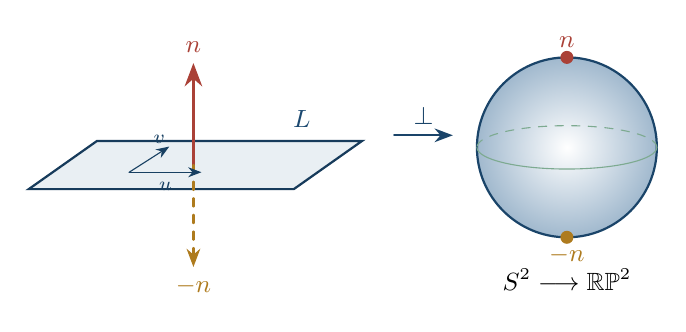
\begin{tikzpicture}[>=Stealth,line cap=round,scale=1.02]
 \filldraw[fill=manifoldblue!10,draw=manifoldblue!65!black,thick]
 (-4.6,-.52)--(-1.3,-.52)--(-.45,.08)--(-3.75,.08)--cycle;
 \draw[->,very thick,manifoldred] (-2.55,-.22)--(-2.55,1.05)
   node[above,font=\small] {$n$};
 \draw[->,thick,manifoldgold!85!black,dashed]
   (-2.55,-.22)--(-2.55,-1.49)
   node[below,font=\small] {$-n$};
 \node[font=\small,manifoldblue!80!black] at (-1.2,.35) {$L$};
 \draw[->,manifoldblue!70!black] (-3.35,-.31)--(-2.45,-.31)
   node[midway,below,font=\scriptsize] {$u$};
 \draw[->,manifoldblue!70!black] (-3.35,-.31)--(-2.85,.01)
   node[near end,above,font=\scriptsize] {$v$};
 \shade[inner color=white,outer color=manifoldblue!43] (2.1,0) circle (1.12);
 \draw[manifoldblue!75!black,thick] (2.1,0) circle (1.12);
 \draw[manifoldgreen!65,thin] (.98,0) arc[start angle=180,end angle=360,x radius=1.12,y radius=.27];
 \draw[manifoldgreen!65,thin,dashed] (3.22,0)
   arc[start angle=0,end angle=180,x radius=1.12,y radius=.27];
 \fill[manifoldred] (2.1,1.12) circle (2.3pt)
   node[above,font=\small] {$n$};
 \fill[manifoldgold!85!black] (2.1,-1.12) circle (2.3pt)
   node[below,font=\small] {$-n$};
 \draw[->,manifoldblue!75!black,thick] (-.05,.15)--(.68,.15)
   node[midway,above,font=\small] {$\perp$};
 \node[font=\small] at (2.1,-1.65) {$S^2\longrightarrow\mathbb{RP}^2$};
\end{tikzpicture}
\caption{Orientacja płaszczyzny w $\R^3$ wybiera jedną z
dwóch jednostkowych normalnych. Zapomnienie orientacji
utożsamia punkty antypodyczne $n$ i $-n$ na sferze.}
\label{fig:grass-normalne}
\end{figure}

\begin{stwierdzenie}[Bazy ortonormalne i przestrzeń ilorazowa]
\label{prop:grass-stiefel}
Niech $V_k(\R^n)$ będzie zbiorem uporządkowanych
ortonormalnych $k$-ramek $(v_1,\ldots,v_k)$.
Odwzorowanie $(v_i)\mapsto\operatorname{span}(v_i)$ ma
włókna izomorficzne z $\mathrm O(k)$.
Ponadto, jako gładkie przestrzenie,
\[
 \operatorname{Gr}_k(\R^n)
   \cong\mathrm O(n)/(\mathrm O(k)\times\mathrm O(n-k)),
\quad
 \operatorname{Gr}_k(\C^n)
   \cong\mathrm U(n)/(\mathrm U(k)\times\mathrm U(n-k)).
\]
\end{stwierdzenie}
\begin{proof}
Dwie ramki wyznaczają tę samą $k$-płaszczyznę wtedy
i tylko wtedy, gdy zmiana bazy między nimi należy do
$\mathrm O(k)$. Wykonując ortonormalizację Grama--Schmidta
na wektorach $u_i+Au_i$ z mapy wykresowej, dostajemy
gładki lokalny wybór ramki; włókna są więc lokalnie
kopiami $\mathrm O(k)$. Grupa $\mathrm O(n)$ działa
tranzytywnie na płaszczyznach: wybieramy bazy ortonormalne
dwóch płaszczyzn, uzupełniamy je do baz $\R^n$ i bierzemy
odwzorowanie przenoszące pierwszą pełną bazę na drugą.
Element zachowujący standardowe $\R^k$ zachowuje też
jego dopełnienie prostopadłe, czyli ma postać blokową
$\mathrm{diag}(B,C)$ z $B\in\mathrm O(k)$,
$C\in\mathrm O(n-k)$. To daje pierwszy iloraz.
Wyjaśnijmy gładką strukturę ilorazu. W rozkładzie ortogonalnym
$P\oplus Q$ uzupełniamy ramkę wykresu przez ramkę
$\Gamma(-A^*)\subset Q\oplus P$ jego dopełnienia prostopadłego:
jej wektory mają postać $-A^*w+w$, $w\in Q$.
Ortonormalizacja obu ramek daje macierz $s(A)\in\mathrm O(n)$
zależną gładko od $A$. Każda macierz ortogonalna nad tą mapą
ma jednoznaczną postać $s(A)\operatorname{diag}(B,C)$.
Parametr $A$ odzyskujemy z obrazu pierwszych $k$ kolumn,
a bloki $B,C$ z iloczynu $s(A)^{-1}O$. Daje to lokalny
produkt i jego gładką odwrotność; po podzieleniu przez bloki
pozostaje dokładnie mapa wykresowa grassmannianu.
Argument dla $\C$ jest taki sam, z bazami unitarnymi,
sprzężeniem hermitowskim i grupą $\mathrm U(n)$.
\end{proof}

Iloczyn zewnętrzny z Sekcji~\ref{sec:algebra-zewnetrzna}
pozwala zapisać $k$-płaszczyznę jednym wielowektorem,
określonym z dokładnością do niezerowego skalara.

\begin{twierdzenie}[Zanurzenie Plückera]
\label{thm:grass-plucker}
Jeśli $(v_1,\ldots,v_k)$ jest bazą $L$, to wzór
\begin{equation}\label{eq:plucker}
 \mathrm{Pl}(L):=[v_1\wedge\cdots\wedge v_k]
 \in\mathbb P(\Lambda^k V)
\end{equation}
określa gładkie zanurzenie
$\operatorname{Gr}_k(V)\hookrightarrow\mathbb P(\Lambda^k V)$.
Nawias $[\xi]$ oznacza prostą $\mathbb K\xi$,
$\xi\ne0$. Obraz składa się dokładnie z klas
niezerowych \emph{wielowektorów prostych}.
\end{twierdzenie}
\begin{proof}
Zmiana bazy $(v_i)$ macierzą $C$ mnoży iloczyn
zewnętrzny przez $\det C\ne0$ na mocy
Twierdzenia~\ref{thm:det-wlasnosci}, więc klasa
projektowa jest dobrze określona. Jeżeli
$\xi=v_1\wedge\cdots\wedge v_k\ne0$, to
\[
 L=\{w\in V:w\wedge\xi=0\}.
\]
Wektory z $L$ dają zero przez powtórzenie czynnika.
Jeśli $w\notin L$, rodzina $(v_1,\ldots,v_k,w)$
jest liniowo niezależna; po uzupełnieniu do bazy
Twierdzenie~\ref{thm:wedge-baza} mówi, że jej
iloczyn zewnętrzny jest niezerowy. Zatem
$\mathrm{Pl}(L)$ wyznacza $L$ jednoznacznie.

Pokażmy, skąd bierze się gładki odwrotny wzór na obrazie.
W mapie $V=P\oplus Q$ wybierzmy bazy
$e_1,\ldots,e_k$ przestrzeni $P$ oraz
$e_{k+1},\ldots,e_n$ przestrzeni $Q$ i zapiszmy
$Ae_j=\sum_{a=1}^{n-k}a_{aj}e_{k+a}$.
W wielowektorze
$\xi_A=(e_1+Ae_1)\wedge\cdots\wedge(e_k+Ae_k)$
współczynnik $p_{1\cdots k}$ wynosi $1$.
Współczynnik przy
$e_1\wedge\cdots\wedge\widehat{e_j}\wedge\cdots
\wedge e_k\wedge e_{k+a}$ wynosi
$(-1)^{k-j}a_{aj}$: przesuwamy $e_{k+a}$
przez $k-j$ późniejszych czynników.
Z ilorazów tych współczynników przez $p_{1\cdots k}$
odzyskujemy wszystkie $a_{aj}$.
W ogólnej mapie projektowej dzielimy przez
odpowiedni niezerowy współczynnik $p_I$.
Odwzorowanie~\eqref{eq:plucker} jest więc gładkie.
Wzory odzyskujące $a_{aj}$ są określone na całym otwartym
zbiorze przestrzeni projektowej $p_{1\cdots k}\ne0$, nie tylko
na obrazie. Ich złożenie z $\mathrm{Pl}$ jest mapą identyczną
w parametrach $A$; różniczkowanie daje lewą odwrotność różniczki
$\mathrm{Pl}$, która jest zatem injektywna.
Otrzymaliśmy immersję. Ponieważ grassmannian jest zwarty,
a przestrzeń projektowa Hausdorffa, ciągła injekcja jest
homeomorfizmem na obraz. To daje zanurzenie i domkniętość obrazu.
\end{proof}

\begin{przyklad}[Relacja Plückera dla $\operatorname{Gr}_2(\R^4)$]
Zapiszmy $\xi=\sum_{1\leq i<j\leq4}p_{ij}e_i\wedge e_j$.
Rozwinięcie $\xi\wedge\xi$ daje
\begin{equation}\label{eq:plucker-24}
 \xi\wedge\xi=
 2(p_{12}p_{34}-p_{13}p_{24}+p_{14}p_{23})
   e_1\wedge e_2\wedge e_3\wedge e_4.
\end{equation}
Jeżeli $\xi=u\wedge v$, to $\xi\wedge\xi=0$,
więc współczynniki spełniają relację w nawiasie.
Odwrotnie, dla $\xi\ne0$ z taką relacją możemy
przestawić współrzędne tak, by $p_{12}\ne0$.
Po podzieleniu przez $p_{12}$ ustawiamy w wykresie
$e_1+ae_3+ce_4$, $e_2+be_3+de_4$ liczby
$b=p_{13}/p_{12}$, $d=p_{14}/p_{12}$,
$a=-p_{23}/p_{12}$, $c=-p_{24}/p_{12}$.
Pięć współczynników się zgadza z definicji,
a szósty jest równy $ad-bc=p_{34}/p_{12}$
właśnie dzięki relacji. To dowodzi również
wystarczalności. Na przykład
$e_1\wedge e_2+e_3\wedge e_4$ ma
$p_{12}p_{34}=1$ i pozostałe wyrazy zerowe,
więc nie jest wielowektorem prostym, zgodnie
z wcześniejszym Przykładem w
Sekcji~\ref{sec:baza-zewnetrzna}.
\end{przyklad}

\begin{twierdzenie}[Odwzorowanie Gaussa i wiązka styczna]
\label{thm:grass-gauss}
Niech $M^m\subset\R^N$ będzie gładką podrozmaitością.
Przypisanie
$G(p)=T_pM\in\operatorname{Gr}_m(\R^N)$
jest gładkim \emph{odwzorowaniem Gaussa}. Wiązki
$TM$ i normalna $\nu M$ są odpowiednio
cofnięciami $G^*\gamma^m$ i $G^*\mathcal Q$
z~\eqref{eq:grass-ciag}.
\end{twierdzenie}
\begin{proof}
W mapie podrozmaitości zapisujemy jej parametryzację
$F:U\subset\R^m\to\R^N$. Wektory
$\partial_iF(x)$ tworzą gładką bazę $T_{F(x)}M$.
W pobliżu ustalonego punktu pewien minor $m\times m$
macierzy $\dd F$ pozostaje niezerowy. W odpowiadającym
mu rozkładzie $\R^N=P\oplus Q$ przestrzeń
$T_{F(x)}M$ jest wykresem macierzy
$A(x)=D_QF(x)(D_PF(x))^{-1}$,
gładkiej w $x$. Stąd $G$ jest gładka.
Włókno $(G^*\gamma^m)_p$ to z definicji
$\gamma^m_{G(p)}=T_pM$; lokalne ramki po obu
stronach są tymi samymi $\partial_iF$.
Włókno $(G^*\mathcal Q)_p$ to
$\R^N/T_pM$, czyli $\nu_pM$ z
Przykładu o wiązce normalnej w Sekcji o podrozmaitościach
Rozdziału~\ref{ch:rozmaitosci}.
Zgodność lokalnych trywializacji daje oba
izomorfizmy wiązek.
\end{proof}

\begin{uwaga}[Dlaczego wiązka tautologiczna jest uniwersalna?]
Na zwartej rozmaitości każdą gładką wiązkę $E$
rzędu $k$ można umieścić w trywialnej wiązce
$M\times\R^N$ dla pewnego $N$.
Oto konstrukcja. Wybieramy skończone pokrycie
trywializujące $U_i$, jego mniejsze podpokrycie
oraz funkcje gładkie $\beta_i$ o nośnikach w $U_i$,
takie że dla każdego $p$ co najmniej jedna
$\beta_i(p)$ jest niezerowa. Jeśli $[v]_i\in\R^k$
oznacza współrzędne $v\in E_p$ na $U_i$,
definiujemy różnowartościowe odwzorowanie liniowe w $v$
\[
 j_p(v)=\bigl(\beta_1(p)[v]_1,\ldots,
                  \beta_r(p)[v]_r\bigr)\in\R^{kr},
\]
przyjmując wartość $0$ dla bloku poza $U_i$.
Podparcie $\beta_i$ wewnątrz $U_i$ zapewnia
gładkość po przedłużeniu zerem; co najmniej
jeden niezerowy blok zapewnia iniektywność $j_p$.
Obrazy $j_p(E_p)$ zmieniają się gładko, ponieważ
lokalnie tworzą kolumny macierzy gładkiej i
stałego rzędu $k$, a więc definiują odwzorowanie
$f:M\to\operatorname{Gr}_k(\R^{kr})$.
Wprost z definicji włókien mamy
$E\cong f^*\gamma^k$. Ta konkretna konstrukcja
wyjaśnia użyteczność grassmannianów dla topologii
wiązek; nie potrzebuje jeszcze teorii klas
charakterystycznych.
\end{uwaga}

\section{Algebra Clifforda: iloczyn i dowód wymiaru}
\label{sec:clifford}

Od tego miejsca $V$ jest rzeczywistą przestrzenią
euklidesową wymiaru $n$ z iloczynem skalarnym
$\langle\cdot,\cdot\rangle$ i normą
$\|v\|^2=\langle v,v\rangle$. Algebra zewnętrzna
pamięta zorientowane pola: $v\wedge v=0$.
Algebra Clifforda pamięta ponadto \emph{długość}:
kwadrat wektora jest skalarem $-\|v\|^2$.
Przyjmujemy konsekwentnie ten znak minus;
w literaturze spotyka się również konwencję przeciwną.

\begin{definicja}[Algebra Clifforda]
\index{algebra clifforda@Algebra Clifforda}
\label{def:clifford}
Niech $I_q$ będzie ideałem obustronnym algebry
tensorowej $T(V)$ z Definicji~\ref{def:algebra-tensorowa},
generowanym przez
$v\otimes v+\|v\|^2\,1$ dla wszystkich $v\in V$.
\emph{Algebra Clifforda} to
\[
 \operatorname{Cl}(V):=T(V)/I_q.
\]
Obraz $v\in V$ oznaczamy nadal $v$,
a mnożenie w ilorazie zapisujemy bez symbolu $\otimes$.
Z definicji $v^2=-\|v\|^2\,1$.
\end{definicja}

Po usunięciu z relacji składnika $\|v\|^2\,1$
otrzymujemy algebrę zewnętrzną
(Definicja~\ref{def:algebra-zewnetrzna}).
Tak więc obie algebry startują z tej samej algebry
tensorowej; zmieniamy tylko relację, przez którą
dzielimy. W algebrze Clifforda nie można zachować
zwykłego stopnia tensorowego: relacja utożsamia
wyraz stopnia $2$ ze skalarem stopnia $0$.
Pozostaje rozróżnienie stopnia \emph{parzystego}
i \emph{nieparzystego}, bo oba wyrazy relacji
mają tę samą parzystość.

\begin{twierdzenie}[Relacja Clifforda i własność uniwersalna]
\label{thm:cliff-relacje}
Dla $v,w\in V$ w $\operatorname{Cl}(V)$ zachodzi
\begin{equation}\label{eq:cliff-relacja}
 vw+wv=-2\langle v,w\rangle\,1.
\end{equation}
Jeżeli $\mathcal A$ jest łączną algebrą rzeczywistą
z jedynką, a $f:V\to\mathcal A$ jest liniowa i spełnia
$f(v)^2=-\|v\|^2 1_{\mathcal A}$ dla każdego $v$,
to istnieje dokładnie jeden homomorfizm algebr
$\widehat f:\operatorname{Cl}(V)\to\mathcal A$
przedłużający $f$.
\end{twierdzenie}
\begin{proof}
Rozwijając $(v+w)^2$ na dwa sposoby, otrzymujemy
\[
 v^2+vw+wv+w^2=-\|v+w\|^2\,1
  =-(\|v\|^2+\|w\|^2+2\langle v,w\rangle)\,1.
\]
Po odjęciu $v^2=-\|v\|^2 1$ i
$w^2=-\|w\|^2 1$ zostaje~\eqref{eq:cliff-relacja}.
Z Twierdzenia~\ref{thm:algebra-tensorowa-universal}
odwzorowanie $f$ przedłuża się jednoznacznie do homomorfizmu
$F:T(V)\to\mathcal A$. Dla każdego generatora ideału
$I_q$ mamy
$F(v\otimes v+\|v\|^2 1)
 =f(v)^2+\|v\|^2 1_{\mathcal A}=0$.
Jądro homomorfizmu jest ideałem, więc zawiera $I_q$.
Wobec tego wzór $\widehat f([t])=F(t)$
nie zależy od przedstawiciela $t\in T(V)$
i wyznacza żądany homomorfizm na ilorazie.
Jednoznaczność wynika stąd, że $V$ i jedynka
generują $\operatorname{Cl}(V)$.
\end{proof}

Przy bazie ortonormalnej $(e_1,\ldots,e_n)$
relacja~\eqref{eq:cliff-relacja} mówi
\begin{equation}\label{eq:cliff-orto}
 e_i^2=-1,\qquad e_ie_j=-e_je_i\quad(i\ne j).
\end{equation}
Stąd każdy iloczyn generatorów można uporządkować
rosnąco, redukując powtórzone indeksy.
Trudniejszą częścią jest wykazanie, że tak otrzymane
wyrazy nie mają dodatkowych relacji.

\begin{twierdzenie}[Baza algebry Clifforda]
\label{thm:cliff-baza}
Dla bazy ortonormalnej $e_1,\ldots,e_n$ elementy
\[
 1,\qquad e_{i_1}\cdots e_{i_r}
 \quad(1\leq i_1<\cdots<i_r\leq n,\ 1\leq r\leq n)
\]
stanowią bazę $\operatorname{Cl}(V)$. Zatem
$\dim_\R\operatorname{Cl}(V)=2^n$.
Dla $n\geq1$ części parzysta i nieparzysta mają
po $2^{n-1}$ wymiarów.
\end{twierdzenie}
\begin{proof}
\emph{Rozpinanie.} Obrazy słów $v_1\cdots v_r$
rozpinają iloraz $T(V)/I_q$. Po rozwinięciu każdego
$v_j$ w bazie wystarczą słowa z liter $e_i$.
Równości~\eqref{eq:cliff-orto} pozwalają zamienić
każde dwie sąsiednie różne litery (ze zmianą znaku)
i usunąć parę równych liter ($e_i^2=-1$).
Powtarzając te operacje, dostajemy kombinację
iloczynów o rosnących, różnych indeksach.

\emph{Niezależność.} Skorzystamy z algebry zewnętrznej
$\Lambda(V)$ z Rozdziału~\ref{ch:algebra-tensorowa}.
Na niej określmy dwie operacje:
\[
 \varepsilon(v)\omega:=v\wedge\omega,\qquad
 \iota_v(w_1\wedge\cdots\wedge w_r)
 :=\sum_{j=1}^r(-1)^{j-1}
   \langle v,w_j\rangle\,
   w_1\wedge\cdots\wedge\widehat{w_j}
       \wedge\cdots\wedge w_r .
\]
Kreska nad $w_j$ oznacza pominięcie tego czynnika;
przyjmujemy $\iota_v(1)=0$.
Wzór na $\iota_v$ jest wieloliniowy i alternujący
w $w_j$: przy zamianie dwóch sąsiednich argumentów składniki
pomijające inny argument zmieniają znak przez antysymetrię iloczynu
zewnętrznego, a dwa pozostałe zamieniają się miejscami z przeciwnymi
znakami. Zatem własność uniwersalna
z Twierdzenia~\ref{thm:wedge-multilinear}
zapewnia, że operator jest dobrze określony.
Bezpośrednio z tego wzoru otrzymujemy
\[
 \iota_v(w\wedge\omega)
  =\langle v,w\rangle\omega-w\wedge\iota_v\omega.
\]
Pierwszy składnik powstaje przy usunięciu pierwszego
czynnika; pozostałe mają o jeden minus więcej niż
w $\iota_v\omega$. Usunięcie dwóch czynników
w dwóch przeciwnych kolejnościach daje składniki
o przeciwnych znakach, zatem $\iota_v^2=0$.
Również $\varepsilon(v)^2=0$, bo $v\wedge v=0$.
Jeżeli $c(v):=\varepsilon(v)-\iota_v$, to
\[
 c(v)^2
 =-\bigl(\varepsilon(v)\iota_v
          +\iota_v\varepsilon(v)\bigr)
 =-\|v\|^2\id_{\Lambda(V)}.
\]
Własność uniwersalna z poprzedniego twierdzenia
daje więc reprezentację
$c:\operatorname{Cl}(V)\to\operatorname{End}_\R(\Lambda V)$.
Przyłóżmy ją do $1\in\Lambda^0V$.
Dla różnych ortonormalnych $e_{i_j}$ wszystkie
kontrakcje pojawiające się podczas kolejnego
działania znikają: nowy $e_{i_j}$ jest prostopadły
do wcześniej utworzonych czynników. Stąd
\[
 c(e_{i_1}\cdots e_{i_r})\,1
    =e_{i_1}\wedge\cdots\wedge e_{i_r},\qquad
 c(1)\,1=1.
\]
Prawa strona przebiega bazę $\Lambda(V)$ z
Twierdzenia~\ref{thm:wedge-baza}. Jeśli kombinacja
uporządkowanych słów znikałaby w algebrze Clifforda,
jej działanie na $1$ dawałoby zerową kombinację
\emph{różnych} wektorów tej bazy. Wszystkie
współczynniki muszą więc być zerowe.
Słów o $r$ indeksach jest $\binom nr$;
sumując po $r$ otrzymujemy $2^n$.
Wreszcie bijekcja $I\mapsto I\triangle\{1\}$
zamienia podzbiory parzystej i nieparzystej
liczności, co dowodzi równości ich liczby.
\end{proof}

\begin{uwaga}[Podobne przestrzenie, różne mnożenia]
\label{rem:cliff-zewnetrzna}
Istnieje kanoniczny izomorfizm \emph{przestrzeni liniowych}
$\Lambda V\cong\operatorname{Cl}(V)$: wysyła
$v_1\wedge\cdots\wedge v_r$ na antysymetryzację
$\frac1{r!}\sum_{\sigma\in S_r}\operatorname{sgn}(\sigma)
 v_{\sigma(1)}\cdots v_{\sigma(r)}$.
Jest dobrze określony, bo wyrażenie jest alternujące;
na bazowych wektorach ortonormalnych daje
$e_{i_1}\cdots e_{i_r}$, więc poprzednie twierdzenie
zapewnia odwracalność. Nie jest to jednak izomorfizm
algebr: w $\Lambda V$ mamy $v\wedge v=0$,
a w $\operatorname{Cl}(V)$ mamy
$v^2=-\|v\|^2$. To wyjaśnia, dlaczego obie
przestrzenie mają wymiar $2^n$, choć kodują
inne mnożenia.
\end{uwaga}

\begin{przyklad}[Wymiary $0$, $1$ i $2$]
Dla $V=0$ otrzymujemy $\operatorname{Cl}(0)=\R$.
W wymiarze $1$, przy $e_1^2=-1$, każdy element
ma postać $a+be_1$ i mnoży się jak liczba
$a+bi\in\C$. Stąd $\operatorname{Cl}(\R)\cong\C$
\emph{jako algebra rzeczywista}.
W wymiarze $2$ baza $(1,e_1,e_2,e_1e_2)$
spełnia dokładnie relacje kwaternionów:
$e_1\leftrightarrow i$, $e_2\leftrightarrow j$,
$e_1e_2\leftrightarrow k$, zatem
$\operatorname{Cl}(\R^2)\cong\mathbb H$.
Na przykład $(e_1+2e_2)^2=-5$, podczas gdy
$(e_1+2e_2)\wedge(e_1+2e_2)=0$
w algebrze zewnętrznej. Porównujemy więc kwadraty tego samego wektora.
\end{przyklad}

\begin{stwierdzenie}[Iloczyn wektorów: skalar i dwuwektor]
\label{prop:cliff-wedge}
Przez powyższy izomorfizm przestrzeni liniowych
iloczyn Clifforda dwóch wektorów rozkłada się na
\begin{equation}\label{eq:cliff-rozdzial}
 vw=-\langle v,w\rangle
       +\tfrac12(vw-wv)
 \quad\longleftrightarrow\quad
 -\langle v,w\rangle+v\wedge w.
\end{equation}
\end{stwierdzenie}
\begin{proof}
Suma $vw+wv$ jest równa
$-2\langle v,w\rangle$ z~\eqref{eq:cliff-relacja}.
Dodając połowę tej sumy do połowy różnicy,
odzyskujemy $vw$. Antysymetryzacja
$v\wedge w\mapsto\tfrac12(vw-wv)$
jest przypadkiem stopnia $2$ opisanym w
poprzedniej uwadze.
\end{proof}

\begin{figure}[!htbp]
\centering
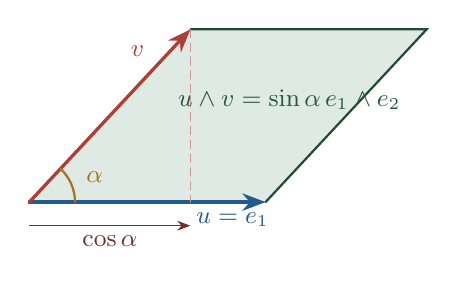
\begin{tikzpicture}[>=Stealth,line cap=round,scale=1.0]
 \coordinate (O) at (0,0);
 \coordinate (U) at (3.0,0);
 \coordinate (W) at ({3*cos(47)},{3*sin(47)});
 \coordinate (UW) at ({3+3*cos(47)},{3*sin(47)});
 \fill[manifoldgreen!16] (O)--(U)--(UW)--(W)--cycle;
 \draw[manifoldgreen!60!black,thick] (U)--(UW)--(W);
 \draw[->,manifoldblue,very thick] (O)--(U)
  node[pos=.86,below,font=\small] {$u=e_1$};
 \draw[->,manifoldred,very thick] (O)--(W)
  node[pos=.78,above left,font=\small] {$v$};
 \draw[densely dashed,manifoldred!55] (W)--({3*cos(47)},0);
 \draw[->,manifoldred!70!black] (0,-.3)--({3*cos(47)},-.3)
  node[midway,below,font=\small] {$\cos\alpha$};
 \draw[manifoldgold!80!black,thick] (.58,0)
  arc[start angle=0,end angle=47,radius=.58];
 \node[manifoldgold!80!black,font=\small] at (.83,.32) {$\alpha$};
 \node[manifoldgreen!70!black,font=\small] at (3.3,1.3)
  {$u\wedge v=\sin\alpha\,e_1\wedge e_2$};
\end{tikzpicture}
\caption{Dla jednostkowych $u=e_1$ i
$v=\cos\alpha\,e_1+\sin\alpha\,e_2$ iloczyn Clifforda
$uv=-\cos\alpha+\sin\alpha\,e_1e_2$ łączy
ujemny iloczyn skalarny ze zorientowanym polem.}
\label{fig:cliff-iloczyn}
\end{figure}

\section{Od odbić do grupy Spin}
\label{sec:spin-grupa}

Ustalmy najpierw dwie operacje na algebrze Clifforda.
Zmiana każdego $v$ na $-v$ zachowuje relacje definiujące,
więc daje automorfizm $\alpha$, z $\alpha^2=\id$.
Jego przestrzenie własne dla $+1$ i $-1$ są rozpięte
odpowiednio przez słowa parzyste i nieparzyste; dowód bazy
pokazuje, że ich suma jest prosta.
Drugą operacją jest \emph{rewersja}, oznaczana tyldą:
\[
 \widetilde{v_1\cdots v_r}=v_r\cdots v_1,\qquad
 \widetilde 1=1,
\]
przedłużona liniowo. Jest dobrze określona na ilorazie:
odwracanie słów w $T(V)$ ustala każdy generator
$v\otimes v+\|v\|^2 1$, a element $a(v\otimes v+\|v\|^2 1)b$
wysyła na $\widetilde b(v\otimes v+\|v\|^2 1)\widetilde a$,
nadal należący do ideału. Zatem
$\widetilde{st}=\widetilde t\,\widetilde s$ i
$\widetilde{\widetilde s}=s$, niezależnie od zapisu $s$ jako sumy słów.

Odbicie względem hiperpłaszczyzny prostopadłej
do jednostkowego $u\in V$ ma wzór
\begin{equation}\label{eq:spin-odbicie}
 r_u(v)=v-2\langle u,v\rangle u.
\end{equation}
Rozkład $v=\langle u,v\rangle u+w$, $w\perp u$,
pokazuje, że $r_u$ odwraca składową równoległą do $u$
i zostawia składową $w$. Jego wyznacznik jest równy $-1$.
Relacja Clifforda daje zaskakujący opis tego odbicia:
ponieważ $u^2=-1$, mamy $u^{-1}=-u$ i
\[
 -uvu^{-1}=uvu
 =-\langle u,v\rangle u+w
 =r_u(v).
\]

\begin{definicja}[Grupa Pin]
\label{def:pin-grupa}
\index{grupa pin@Grupa Pin}
Dla euklidesowej przestrzeni $V$ grupą $\operatorname{Pin}(V)$
nazywamy podgrupę odwracalnych elementów $\operatorname{Cl}(V)$
złożoną ze wszystkich skończonych iloczynów wektorów
jednostkowych; dopuszczamy pusty iloczyn $1$.
W odróżnieniu od grupy Spin dopuszczamy także nieparzystą
liczbę czynników. Dla $s\in\operatorname{Pin}(V)$ określamy
\[
 \rho_{\mathrm{Pin}}(s)(v):=\alpha(s)v s^{-1},
 \qquad v\in V,
\]
gdzie $\alpha$ zmienia znak każdego wektora, jak wyżej.
\end{definicja}

Wzór jest skręconym sprzężeniem: dla jednostkowego $u$
daje $\rho_{\mathrm{Pin}}(u)(v)=-uvu^{-1}=r_u(v)$.
Zatem pojedynczy wektor reprezentuje odbicie, a jego parzysty
iloczyn reprezentuje obrót. Na przykład w $\R^2$ element
$e_1\in\operatorname{Pin}(2)$ daje odbicie w prostej
$e_1^\perp$, podczas gdy $e_1e_2$ daje obrót o pół obiegu.
Przy przyjętej relacji $u^2=-\|u\|^2$ grupa ta bywa
oznaczana $\operatorname{Pin}^{-}(n)$; znak rozróżnia dwie
konwencje algebry Clifforda.

\begin{definicja}[Grupa Spin]
\index{grupa spin@Grupa Spin}
\label{def:spin-grupa}
Niech $n=\dim V\geq2$. \emph{Grupą spinową}
$\operatorname{Spin}(V)$ nazywamy podgrupę
odwracalnych elementów $\operatorname{Cl}(V)$,
składającą się z iloczynów \emph{parzystej}
liczby wektorów jednostkowych:
\[
 \operatorname{Spin}(V)
 :=\{u_1\cdots u_{2r}:\|u_j\|=1,\ r\geq0\}.
\]
Pusty iloczyn to $1$. Skrót
$\operatorname{Spin}(n)$ oznacza
$\operatorname{Spin}(\R^n)$ ze standardową metryką.
Dla $s\in\operatorname{Spin}(V)$ określamy
$\rho(s)v:=svs^{-1}$.
Topologię na grupie bierzemy z jej włączenia do skończenie
wymiarowej przestrzeni $\operatorname{Cl}(V)$. Gładką strukturę
zgodną z tym włączeniem uzasadnimy w dowodzie nakrycia.
\end{definicja}

Zbiór w definicji jest grupą: iloczyn dwóch słów
parzystych jest parzysty, a odwrotność słowa
$u_1\cdots u_{2r}$ to
$(-u_{2r})\cdots(-u_1)$, ponownie słowo parzyste
złożone z wektorów jednostkowych.
Każdy jego czynnik ma dobrze określoną odwrotność.

\begin{twierdzenie}[Dwukrotne nakrycie grupy obrotów]
\label{thm:spin-nakrycie}
Przypisanie $\rho$ jest surjektywnym homomorfizmem
\[
 \rho:\operatorname{Spin}(n)\longrightarrow\mathrm{SO}(n),
 \qquad\ker\rho=\{1,-1\}.
\]
Jest gładkim dwukrotnym nakryciem: każdy obrót
ma dokładnie dwa podniesienia $s$ i $-s$.
\end{twierdzenie}
\begin{proof}
\emph{Dlaczego obrazem jest obrót?}
Dla słowa $s=u_1\cdots u_{2r}$ zastosujmy
wzór na odbicie do kolejnych czynników.
W odwzorowaniu $v\mapsto-u v u^{-1}$ pojawia się
jedno odbicie $r_u$; przy parzystej liczbie
czynników wszystkie minusy się znoszą i
\[
 \rho(s)=r_{u_1}\circ\cdots\circ r_{u_{2r}}.
\]
To złożenie zachowuje iloczyn skalarny i ma
wyznacznik $(-1)^{2r}=1$. Ponieważ
$\rho(st)(v)=s(tvt^{-1})s^{-1}$,
$\rho$ jest homomorfizmem do $\mathrm{SO}(n)$.

\emph{Dlaczego jest surjektywna?}
Pokażmy elementarnie, że każdą izometrię liniową
można zapisać jako iloczyn odbić. Weźmy bazę
ortonormalną $e_1,\ldots,e_n$ i $A\in\mathrm O(n)$.
Jeśli $Ae_1\ne e_1$, to dla
$u=(Ae_1-e_1)/\|Ae_1-e_1\|$ rachunek z
\eqref{eq:spin-odbicie} daje $r_u(Ae_1)=e_1$:
licznik iloczynu
$\langle Ae_1-e_1,Ae_1\rangle$ to
$1-\langle Ae_1,e_1\rangle$, a kwadrat
mianownika to $2(1-\langle Ae_1,e_1\rangle)$.
Jeśli $Ae_1=e_1$, pomijamy ten krok.
Nowa izometria zachowuje $e_1$, więc działa
na $e_1^\perp$. Powtarzamy argument dla $e_2$
w tym dopełnieniu, potem dla $e_3$, itd.
Po skończenie wielu krokach otrzymujemy
identyczność. Zapisujemy więc $A$ jako
iloczyn odbić. Ponieważ $\det A=1$, liczba
użytych odbić musi być parzysta; odpowiadający
im iloczyn jednostkowych $u_j$ jest szukanym
elementem $\operatorname{Spin}(n)$.

\emph{Dlaczego jądro ma tylko dwa elementy?}
Niech $s$ działa trywialnie na $V$. Wtedy
$se_j=e_js$ dla każdego wektora bazy ortonormalnej.
Rozwińmy $s$ w bazie z
Twierdzenia~\ref{thm:cliff-baza}, używając tylko
słów parzystej długości:
$s=\sum_{|I|\ {\rm parzyste}}a_I e_I$.
Dla parzystego niepustego $I$ i $j\in I$
relacja~\eqref{eq:cliff-orto} daje
$e_je_Ie_j^{-1}=-e_I$; gdy $j\notin I$,
otrzymujemy $+e_I$. Równość
$e_jse_j^{-1}=s$ dla \emph{wszystkich} $j$
wymusza więc $a_I=0$ dla każdego niepustego $I$.
Zatem $s=a\,1$. Aby ustalić $a$, odwróćmy
porządek wektorów w słowie:
$\widetilde s=u_{2r}\cdots u_1$.
Wtedy $s\widetilde s=(-1)^{2r}=1$,
bo wektory są jednostkowe i $u_i^2=-1$.
Dla skalarnego $s=a$ również $\widetilde s=a$,
stąd $a^2=1$. Oba znaki występują,
gdyż $-1=e_1e_1\in\operatorname{Spin}(n)$.

\emph{Dlaczego rzeczywiście jest to nakrycie?}
Pokażmy, że w pobliżu identyczności obroty mają
gładko wybrane podniesienie. Dla bliskich
jednostkowych $a,b$ połóżmy
\[
 R(a,b):=-\frac{a+b}{\|a+b\|}\,a
       =\frac{1-ba}{\|a+b\|}\in\operatorname{Spin}(n).
\]
Jest to iloczyn dwóch jednostkowych wektorów,
zależy gładko od $(a,b)$, spełnia $R(a,a)=1$
i przenosi $a$ na $b$: pierwsze odbicie w
hiperpłaszczyźnie do $a$ wysyła $a$ na $-a$,
drugie, o normalnej $(a+b)/\|a+b\|$, wysyła
$-a$ na $b$. Jeśli $A$ jest bliski identyczności,
stosujemy taki rotor, aby skorygować $Ae_1$ do
$e_1$. Otrzymany obrót zachowuje $e_1$.
W $e_1^\perp$ korygujemy następnie obraz
$e_2$, potem $e_3$, kończąc na $e_{n-1}$;
ostatni wektor jest ustalony dzięki wyznacznikowi
$1$. Każdy rotor zależy gładko od $A$
w niewielkim otoczeniu identyczności.
Odwrotność ich iloczynu daje gładką lokalną
sekcję $\sigma$ odwzorowania $\rho$.
Przy innym obrocie przenosimy to otoczenie
przez ustalony element z jego przeciwobrazu.
Jądro $\{\pm1\}$ oznacza, że przeciwobraz
takiego dostatecznie małego otoczenia jest
sumą rozłącznych kopii obrazu $\sigma$ i $-\sigma$.
Są one otwarte w $\operatorname{Spin}(n)$:
blisko $1$ dwie wartości $\pm\sigma(A)$
odróżnia znak współczynnika skalarnego
w algebrze Clifforda, a blisko pozostałych
punktów korzystamy z mnożenia przez
ustalone podniesienie. To jest dokładnie definicja
dwukrotnego nakrycia.
W ten sposób otrzymujemy także atlas gładki: na każdym płacie
używamy współrzędnych z $\mathrm{SO}(n)$ przeniesionych przez $\rho$.
Jest on zgodny z włączeniem do algebry Clifforda. Istotnie,
$\sigma$ jest gładka jako mapa do tej algebry, a pochodna
$\rho\circ\sigma=\id$ jest identycznością. Do różniczkowania
$\rho$ w otoczeniu płata wystarczy gładki wzór
$s\mapsto(v\mapsto\operatorname{pr}_V(svs^{-1}))$
na otwartym zbiorze elementów odwracalnych; na grupie Spin
rzut $\operatorname{pr}_V$ niczego nie zmienia.
Wynika stąd injektywność różniczki $\sigma$, więc płaty są
lokalnie podrozmaitościami algebry Clifforda. Mnożenie jest
dwuliniowe, a odwracanie gładkie: można je obliczać przez
odwracanie macierzy lewego mnożenia. Obie operacje ograniczają
się więc do gładkich operacji grupy Spin, a $\rho$ jest lokalnym dyfeomorfizmem.
\end{proof}

\begin{wniosek}[Nakrycie grupy ortogonalnej przez Pin]
\label{cor:pin-nakrycie}
Dla $n\geq2$ odwzorowanie
\[
 \rho_{\mathrm{Pin}}:\operatorname{Pin}(n)\longrightarrow
 \mathrm O(n)
\]
jest surjektywnym homomorfizmem o jądrze $\{1,-1\}$.
Jest gładkim dwukrotnym nakryciem, a przeciwobraz
$\mathrm{SO}(n)$ jest równy $\operatorname{Spin}(n)$.
\end{wniosek}
\begin{proof}
Automorfizm $\alpha$ jest multiplikatywny, więc
$\rho_{\mathrm{Pin}}(st)=\rho_{\mathrm{Pin}}(s)
\rho_{\mathrm{Pin}}(t)$. Każdy czynnik jednostkowy
daje odbicie. Rozkład izometrii na odbicia wykonano
w dowodzie Twierdzenia~\ref{thm:spin-nakrycie}; zapewnia
on surjektywność. Wyznacznik obrazu iloczynu $r$
wektorów wynosi $(-1)^r$. Parzyste słowa tworzą
zatem dokładnie przeciwobraz $\mathrm{SO}(n)$, czyli
$\operatorname{Spin}(n)$. Element jądra musi być parzysty,
a jądro na $\operatorname{Spin}(n)$ obliczono w tym samym
twierdzeniu jako $\{\pm1\}$. Lokalnie nad składową
$\mathrm{SO}(n)$ mamy już dwa gładkie płaty nakrycia Spin.
Mnożenie przez ustalony wektor jednostkowy przenosi je
na drugą składową $\mathrm O(n)$, co dowodzi ostatniej tezy.
\end{proof}

\begin{przyklad}[Dlaczego pojawia się połowa kąta?]
\label{prz:spin2}
W płaszczyźnie $B=e_1e_2$ spełnia $B^2=-1$.
Ponieważ część parzysta ma bazę $(1,B)$,
jej elementy mają postać $a+bB$. Dla słów
należących do $\operatorname{Spin}(2)$ równość
$s\widetilde s=1$ z poprzedniego dowodu daje
$a^2+b^2=1$. Odwrotnie, jeśli
$a=\cos t$, $b=\sin t$, to
\[
 a+bB=(-\cos t\,e_1-\sin t\,e_2)e_1,
\]
czyli iloczyn dwóch jednostkowych wektorów.
Grupa $\operatorname{Spin}(2)$ jest zatem okręgiem.
Połóżmy
\[
 s_\theta=\cos(\theta/2)+\sin(\theta/2)B.
\]
Korzystając z $Be_1=e_2$ i $Be_2=-e_1$,
obliczamy bez pomijania kroku
\[
 s_\theta e_1s_\theta^{-1}
 =(\cos^2\tfrac\theta2-\sin^2\tfrac\theta2)e_1
   +2\sin\tfrac\theta2\cos\tfrac\theta2\,e_2
 =\cos\theta\,e_1+\sin\theta\,e_2.
\]
Analogicznie obraz $e_2$ to
$-\sin\theta\,e_1+\cos\theta\,e_2$.
Jeden pełny obrót ma zatem podniesienie
$s_{2\pi}=-1$, a dopiero $s_{4\pi}=1$.
Po utożsamieniu obu grup z okręgiem odwzorowanie
$\rho$ ma postać $z\mapsto z^2$.
\end{przyklad}

\begin{figure}[!htbp]
\centering
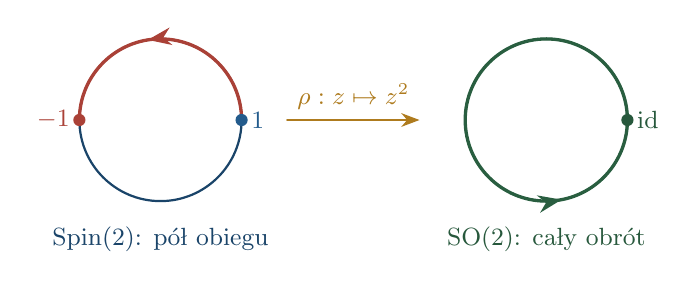
\begin{tikzpicture}[>=Stealth,line cap=round]
 \draw[manifoldblue!75!black,thick] (-2.45,0) circle (1.03);
 \draw[manifoldgreen!75!black,thick] (2.45,0) circle (1.03);
 \draw[manifoldred,very thick,postaction={decorate},
  decoration={markings,mark=at position .55 with {\arrow{Stealth}}}]
  (-1.42,0) arc[start angle=0,end angle=180,radius=1.03];
 \draw[manifoldgreen!75!black,very thick,postaction={decorate},
  decoration={markings,mark=at position .78 with {\arrow{Stealth}}}]
  (3.48,0) arc[start angle=0,end angle=360,radius=1.03];
 \fill[manifoldblue] (-1.42,0) circle (2.2pt)
  node[right,font=\small] {$1$};
 \fill[manifoldred] (-3.48,0) circle (2.2pt)
  node[left,font=\small] {$-1$};
 \fill[manifoldgreen!70!black] (3.48,0) circle (2.2pt)
  node[right,font=\small] {$\id$};
 \draw[->,thick,manifoldgold!85!black] (-.84,0)--(.84,0)
  node[midway,above,font=\small] {$\rho:z\mapsto z^2$};
 \node[font=\small,manifoldblue!75!black] at (-2.45,-1.52)
  {$\operatorname{Spin}(2)$: pół obiegu};
 \node[font=\small,manifoldgreen!70!black] at (2.45,-1.52)
  {$\mathrm{SO}(2)$: cały obrót};
\end{tikzpicture}
\caption{Droga od $1$ do $-1$ w $\operatorname{Spin}(2)$
rzutuje się na pełen obrót w $\mathrm{SO}(2)$.
Końce drogi są różne w grupie Spin, choć odpowiadają
temu samemu obrotowi.}
\label{fig:spin-dwukrotne}
\end{figure}

\begin{przyklad}[Trzy wymiary: kwaterniony]
\label{prz:spin3}
W $\operatorname{Cl}(\R^3)$ część parzysta ma bazę
$1,I=e_2e_3,J=e_3e_1,K=e_1e_2$.
Rachunek przy użyciu~\eqref{eq:cliff-orto} daje
$I^2=J^2=K^2=-1$ i $IJ=K$, $JK=I$, $KI=J$.
Jest to algebra kwaternionów $\mathbb H$.
Odwracanie kolejności czynników wysyła
$a+bI+cJ+dK$ na $a-bI-cJ-dK$,
więc $s\widetilde s=a^2+b^2+c^2+d^2$.
Każdy element $\operatorname{Spin}(3)$
jest zatem jednostkowym kwaternionem.
I odwrotnie, dowolny jednostkowy kwaternion
można zapisać jako $\cos t+\sin t\,B$,
gdzie $B$ jest jednostkowym dwuwektorem
w $\R^3$ (przypadki $\pm1$ są natychmiastowe).
Każdy taki $B$ jest iloczynem dwóch
prostopadłych wektorów jednostkowych. Aby to sprawdzić,
zapiszmy $B=b e_2e_3+c e_3e_1+d e_1e_2$ z $b^2+c^2+d^2=1$.
Wybierzmy jednostkowy $u\perp n=(b,c,d)$ i połóżmy
$v=n\times u$. Wtedy $u,v$ są ortonormalne i $u\times v=n$.
Współczynniki $u\wedge v$ w bazie
$(e_2\wedge e_3,e_3\wedge e_1,e_1\wedge e_2)$ są właśnie $(b,c,d)$,
więc $uv=B$. Z kolei
$\cos t+\sin t\,B$ jest także iloczynem dwóch
wektorów jednostkowych: jeśli $B=uv$ dla
$u\perp v$, to wprost z $vu=-uv$ i $u^2=-1$
otrzymujemy
\[
 (-\cos t\,u-\sin t\,v)u
     =\cos t+\sin t\,uv.
\]
Zatem $\operatorname{Spin}(3)\cong S^3$
jako grupa jednostkowych kwaternionów,
a $\rho:S^3\to\mathrm{SO}(3)$ utożsamia
parę $s,-s$.
\end{przyklad}

\section{Spinory: moduły algebry Clifforda}
\label{sec:spinory}

Wektor w $\R^n$ obraca się przez $\rho(s)\in\mathrm{SO}(n)$.
Spinor ma podlegać działaniu samego $s\in\operatorname{Spin}(n)$,
tak aby dwa podniesienia tego samego obrotu mogły
działać odmiennie. Do opisania wszystkich wymiarów
użyjemy liczb zespolonych. \emph{Zespolenie}
$\operatorname{Cl}^{\C}_n:=
\operatorname{Cl}(\R^n)\otimes_\R\C$
ma tę samą bazę uporządkowanych słów co algebra
rzeczywista, ale współczynniki zespolone.
Jego wymiar nad $\C$ wynosi $2^n$.

\begin{definicja}[Spinor zespolony]
\index{spinor zespolony@Spinor zespolony}
\label{def:spinor}
\emph{Moduł} algebry $A$ nad $\mathbb K$ to przestrzeń liniowa
$\Delta$ nad $\mathbb K$ z działaniem $A\times\Delta\to\Delta$
dwuliniowym nad $\mathbb K$ i zgodnym
z mnożeniem: $(ab)\psi=a(b\psi)$
oraz $1\psi=\psi$. Jest \emph{nieredukowalny},
jeśli $\Delta\ne0$ i nie ma właściwej niezerowej podprzestrzeni
zachowywanej przez wszystkie działania $a\in A$.
W tym rozdziale \emph{przestrzenią spinorów}
w wymiarze $n$ nazwiemy nieredukowalny zespolony
moduł $\Delta_n$ algebry $\operatorname{Cl}^{\C}_n$.
Jej element $\psi$ to spinor. Ograniczenie
działania do $\operatorname{Spin}(n)\subset
\operatorname{Cl}^{\C}_n$ jest
\emph{reprezentacją spinową}.
\end{definicja}

Słowo \emph{moduł} brzmi abstrakcyjnie, lecz tutaj
oznacza po prostu konkretne macierze $c(v)$
działające na kolumny $\psi$, z warunkiem
$c(v)^2=-\|v\|^2 I$. Działanie na całej algebrze
jest wtedy wyznaczone przez jej własność uniwersalną.
Przykładem modułu jest $\Lambda V$ z dowodu
Twierdzenia~\ref{thm:cliff-baza}, ale zwykle jest
on \emph{większy} niż nieredukowalna przestrzeń
spinorów. Nie należy więc utożsamiać automatycznie
wielowektora ze spinorem.

\begin{przyklad}[Macierze Pauliego]
\label{prz:pauli}
Niech
\[
 \sigma_1=\begin{pmatrix}0&1\\1&0\end{pmatrix},
 \quad
 \sigma_2=\begin{pmatrix}0&-i\\i&0\end{pmatrix},
 \quad
 \sigma_3=\begin{pmatrix}1&0\\0&-1\end{pmatrix}.
\]
Bezpośrednie mnożenie daje
$\sigma_i^2=I_2$ i
$\sigma_i\sigma_j=-\sigma_j\sigma_i$ przy $i\ne j$;
na przykład $\sigma_1\sigma_2=i\sigma_3$.
Macierze $c(e_j)=i\sigma_j$ spełniają więc
\[
 c(e_i)c(e_j)+c(e_j)c(e_i)=-2\delta_{ij}I_2.
\]
Dla $n=2$ wystarczą $c(e_1),c(e_2)$.
Ich iloczyn to $-i\sigma_3$, a cztery macierze
$I_2,i\sigma_1,i\sigma_2,-i\sigma_3$
są liniowo niezależne i rozpinają
$M_2(\C)$. Z wymiaru $4$ obu stron dostajemy
$\operatorname{Cl}^{\C}_2\cong M_2(\C)$.
Przestrzeń spinorów $\Delta_2=\C^2$
jest zwykłą przestrzenią kolumn długości $2$.
\end{przyklad}

\begin{twierdzenie}[Klasyfikacja zespolona i wymiar spinorów]
\label{thm:cliff-kompleks}
Dla $m\geq0$ istnieją izomorfizmy algebr
\begin{align}
 \operatorname{Cl}^{\C}_{2m}
   &\cong M_{2^m}(\C), \label{eq:cliff-complex-even}\\
 \operatorname{Cl}^{\C}_{2m+1}
   &\cong M_{2^m}(\C)\oplus M_{2^m}(\C).
   \label{eq:cliff-complex-odd}
\end{align}
Wobec tego nieredukowalny moduł zespolony
ma wymiar $2^{\lfloor n/2\rfloor}$.
Dla parzystego $n$ jest jeden taki moduł
z dokładnością do izomorfizmu, a dla
nieparzystego $n$ są dwa.
\end{twierdzenie}
\begin{proof}
W wymiarze $0$ algebra ma postać $\C$.
W wymiarze $1$ składa się z $a+be_1$ przy
$e_1^2=-1$, więc podstawienia $e_1=i$
i $e_1=-i$ dają
$\operatorname{Cl}^{\C}_1\cong\C\oplus\C$.
Przykład~\ref{prz:pauli} daje
$\operatorname{Cl}^{\C}_2\cong M_2(\C)$.

Wykażmy krok indukcyjny zwiększający wymiar o $2$.
Iloczyn tensorowy algebr wyposażamy tu w mnożenie
$(a\otimes A)(b\otimes B)=ab\otimes AB$, rozszerzone
dwuliniowo; własność uniwersalna iloczynu tensorowego zapewnia
jego poprawne określenie. Łączność sprawdzamy na tensorach
prostych, a jedynką jest $1\otimes I_2$.
Niech $e_1,\ldots,e_n$ będą generatorami
$\operatorname{Cl}^{\C}_n$. W algebrze
$\operatorname{Cl}^{\C}_n\otimes M_2(\C)$
weźmy $n+2$ elementów:
\[
 F_j=e_j\otimes\sigma_3\ (j\leq n),\qquad
 F_{n+1}=1\otimes i\sigma_1,\qquad
 F_{n+2}=1\otimes i\sigma_2.
\]
Każdy $F_j^2=-1$. Dwa różne elementy
antykomutują: dla $j,\ell\leq n$ wynika
to z relacji starych $e_j$; między pierwszymi
$n$ a ostatnimi dwoma wynika z tego, że
$\sigma_3$ antykomutuje z $\sigma_1,\sigma_2$;
ostatnie dwa antykomutują jako macierze Pauliego.
Własność uniwersalna daje homomorfizm
\[
 \operatorname{Cl}^{\C}_{n+2}
    \longrightarrow
   \operatorname{Cl}^{\C}_n\otimes M_2(\C).
\]
Obrazy dwóch ostatnich generatorów dają całą
podalgebrę $1\otimes M_2(\C)$:
ich iloczyn jest $-i(1\otimes\sigma_3)$,
a wraz z jedynką tworzą bazę czterech macierzy.
Następnie z
$(e_j\otimes\sigma_3)(1\otimes\sigma_3)
=e_j\otimes I_2$ otrzymujemy wszystkie
generatory pierwszego czynnika. Homomorfizm
jest więc surjektywny. Obie algebry mają
wymiar $2^{n+2}$ nad $\C$
(Twierdzenie~\ref{thm:cliff-baza}),
więc jest izomorfizmem. Używamy przy tym
$M_d(\C)\otimes M_2(\C)\cong M_{2d}(\C)$:
jednostka macierzowa $E_{ab}\otimes E_{rs}$ odpowiada
jednostce z indeksem wiersza $(a,r)$ i kolumny $(b,s)$.
To bijekcja baz zachowująca mnożenie. Iloczyn tensorowy
rozdziela się też względem sumy prostej obu składników.
Iteracja od $n=0$
i $n=1$ daje~\eqref{eq:cliff-complex-even}
i~\eqref{eq:cliff-complex-odd}.

Pozostaje uzasadnić wymiary modułów. Algebra
$M_d(\C)$ działa na $\C^d$ nieredukowalnie:
jeśli podprzestrzeń zawiera $x\ne0$, to
dla dowolnego $y\in\C^d$ można znaleźć
macierz $A$ z $Ax=y$, więc zawiera wszystkie $y$.
Każdy nieredukowalny moduł $M_d(\C)$ jest
izomorficzny z tym standardowym: wybieramy
wektor $\psi$ z $E_{11}\psi\ne0$ (w razie potrzeby
zmieniamy indeks; jest to możliwe, gdyż
$\sum_jE_{jj}=I$). Wektory
$E_{i1}\psi$, $1\leq i\leq d$, są liniowo
niezależne: zastosowanie $E_{1j}$ do ich
kombinacji liniowej zerowej pozostawia
tylko $j$-ty współczynnik razy
$E_{11}\psi\ne0$. Ich rozpiętość zachowują
wszystkie macierze, bo
$E_{ab}(E_{i1}\psi)=\delta_{bi}E_{a1}\psi$.
Jest zatem niezerowym podmodułem, a
nieredukowalność wymusza, że stanowi cały moduł.
Dla sumy dwóch algebr macierzowych jej
dwa centralne idempotenty $(I,0)$, $(0,I)$
rozkładają każdy moduł na dwie niezmiennicze
części. W module nieredukowalnym tylko jedna
z nich jest niezerowa, co daje dokładnie
dwa wybory modułu wymiaru $d$.
\end{proof}

\begin{uwaga}[Dwa moduły w wymiarze nieparzystym]
Gdy $n=2m+1\geq3$, dwa nieredukowalne moduły
$\operatorname{Cl}^{\C}_n$ są różne, lecz
po ograniczeniu do $\operatorname{Spin}(n)$
dają izomorficzne reprezentacje.
Rzeczywiście, podalgebra parzysta jest
izomorficzna z
$\operatorname{Cl}^{\C}_{n-1}$: przypiszmy
jego generatorowi $e_j$ element $e_je_n$
dla $j<n$. Te elementy mają kwadrat $-1$
i wzajemnie antykomutują, a ponadto
generują wszystkie parzyste słowa
(każde $e_je_\ell$ z $j,\ell<n$ jest
iloczynem odpowiednich $e_je_n$ i $e_\ell e_n$
z dokładnością do znaku). Obie strony mają
wymiar $2^{n-1}$, więc to izomorfizm.
Ponieważ $n-1=2m$, algebra parzysta jest
$M_{2^m}(\C)$ i ma tylko jeden nieredukowalny
moduł. Trzeba jeszcze sprawdzić nieredukowalność ograniczeń:
każdy z dwóch modułów ma wymiar $d=2^m$, a w dowolnym
niezerowym module $M_d(\C)$ konstrukcja z jednostkami $E_{ij}$
z poprzedniego dowodu daje podmoduł wymiaru $d$.
Tutaj musi on być całą przestrzenią. Ponadto słowa parzyste
z wektorów ortonormalnych należą do Spin i rozpinają algebrę
parzystą, więc niezmienniczość względem Spin jest równoważna
niezmienniczości względem tej algebry.
W szczególności spinor dla obrotów
wymiaru $3$ ma po prostu dwie zespolone składowe.
\end{uwaga}

\begin{stwierdzenie}[Spinory chiralne w wymiarze parzystym]
\label{prop:spin-chiral}
Dla $n=2m\geq2$ ustalmy orientację $V$ i dodatnią bazę
ortonormalną $(e_1,\ldots,e_{2m})$. W module $\Delta_{2m}$
element
\[
 \Gamma:=i^m c(e_1e_2\cdots e_{2m})
\]
ma własność $\Gamma^2=I$, komutuje z działaniem
$\operatorname{Spin}(2m)$ i dzieli przestrzeń
na dwa podmoduły dla grupy Spin:
\[
 \Delta_{2m}=\Delta^+_{2m}\oplus\Delta^-_{2m},
 \qquad
 \Delta^\pm_{2m}=\ker(\Gamma\mp I),\qquad
 \dim_\C\Delta^\pm_{2m}=2^{m-1}.
\]
Nazywamy je \emph{półspinorami}.
\end{stwierdzenie}
\begin{proof}
Niech $\omega=e_1\cdots e_{2m}$. Aby uporządkować czynniki
w iloczynie $\omega^2$, wykonujemy $(2m)(2m-1)/2$ transpozycji;
następnie mnożymy $2m$ kwadratów $e_j^2=-1$.
Otrzymujemy
$\omega^2=(-1)^{m(2m-1)}(-1)^{2m}=(-1)^m$.
Ponieważ $i^{2m}=(-1)^m$, mamy $\Gamma^2=I$.
Zatem $P_\pm=\tfrac12(I\pm\Gamma)$ są projekcjami
o sumie $I$ i zerowym iloczynie; dają podany rozkład na przestrzenie własne.
Zmiana dodatniej bazy ortonormalnej nie zmienia $\omega$:
jej iloczyn jest antysymetryzacją najwyższego iloczynu zewnętrznego,
a ten zmienia się o wyznacznik, równy $1$.
Przy odwróceniu orientacji $\Gamma$ zmienia znak i oznaczenia
$\Delta^+$, $\Delta^-$ zamieniają się miejscami.
Przesunięcie dowolnego $e_j$ przez pozostałe
$2m-1$ generatory zmienia znak:
$\Gamma c(e_j)=-c(e_j)\Gamma$.
Zatem $\Gamma$ komutuje z iloczynami
parzystej liczby generatorów, w szczególności
ze $\operatorname{Spin}(2m)$; obie przestrzenie
własne są niezmiennicze. Operator
$c(e_1)$ jest odwracalny i przestawia
te przestrzenie własne, więc mają równe
wymiary. Suma wymiarów to $2^m$ z poprzedniego
twierdzenia, co daje $2^{m-1}$.
\end{proof}

\begin{przyklad}[Półspinory w płaszczyźnie]
Dla $n=2$ w modelu Pauliego
$\Gamma=i\,c(e_1)c(e_2)=\sigma_3$,
więc $\Delta^+_2=\C\binom10$ oraz
$\Delta^-_2=\C\binom01$.
Element $s_\theta$ z Przykładu~\ref{prz:spin2}
działa przez
\[
 c(s_\theta)=
 \begin{pmatrix}
  e^{-i\theta/2}&0\\0&e^{i\theta/2}
 \end{pmatrix}.
\]
Wektor po obrocie o $2\pi$ wraca do swego
położenia, a każdy z obu półspinorów
zostaje przemnożony przez $-1$.
\end{przyklad}

\begin{przyklad}[Spinor w $\R^3$ i sfera Blocha]
\label{prz:bloch}
W wymiarze $3$ działanie
$c(e_j)=i\sigma_j$ na $\Delta_3=\C^2$
spełnia relacje Clifforda. Na parzystych
generatorach z Przykładu~\ref{prz:spin3}
otrzymujemy macierze $-i\sigma_1,-i\sigma_2,
-i\sigma_3$. Dla
$s=a+bI+cJ+dK\in\operatorname{Spin}(3)$
macierz działania ma postać
\[
 U_s=aI_2-i(b\sigma_1+c\sigma_2+d\sigma_3).
\]
Z relacji Pauliego dostajemy
$U_s^*U_s=(a^2+b^2+c^2+d^2)I_2=I_2$
oraz $\det U_s=1$. Każda macierz z
$\mathrm{SU}(2)$ ma taką postać: z warunków
unitarności i wyznacznika $1$ wynika
$U=\begin{psmallmatrix}\alpha&\beta\\
-\overline\beta&\overline\alpha\end{psmallmatrix}$,
gdzie $|\alpha|^2+|\beta|^2=1$; cztery
rzeczywiste części $\alpha,\beta$ odpowiadają
jedynej czwórce $(a,b,c,d)$.
Zatem $\operatorname{Spin}(3)\cong\mathrm{SU}(2)$.

Niech teraz $\psi=(z_1,z_2)^T$ ma normę $1$.
Liczby rzeczywiste
\begin{equation}\label{eq:spin-bloch}
 b_j(\psi):=\psi^*\sigma_j\psi
 \quad\text{dają}\quad
 b(\psi)=
 \bigl(2\operatorname{Re}(\overline z_1z_2),
       2\operatorname{Im}(\overline z_1z_2),
       |z_1|^2-|z_2|^2\bigr).
\end{equation}
Rachunek daje
$\|b(\psi)\|^2=
4|z_1|^2|z_2|^2+(|z_1|^2-|z_2|^2)^2=1$.
Zmiana fazy $\psi\mapsto e^{i\varphi}\psi$
nie zmienia $b(\psi)$. Odwrotnie, liczby
$b_j$ wyznaczają macierz
$\psi\psi^*=\frac12(I_2+\sum_jb_j\sigma_j)$,
a ta macierz wyznacza prostą $\C\psi$.
Każdy punkt sfery otrzymujemy: dla
$b=(x,y,z)$ z $z>-1$ bierzemy
$z_1=\sqrt{(1+z)/2}$,
$z_2=(x+iy)/\sqrt{2(1+z)}$;
dla bieguna południowego bierzemy $(0,1)$.
Otrzymujemy więc konkretną identyfikację
\[
 \mathbb{CP}^1=\operatorname{Gr}_1(\C^2)\cong S^2.
\]
Jest to także gładka identyfikacja: na mapie $[1:w]$
wzór ma postać
$b=(2\operatorname{Re}w,2\operatorname{Im}w,1-|w|^2)/(1+|w|^2)$,
a odwrotność poza biegunem południowym to $w=(x+iy)/(1+z)$;
druga mapa analogicznie obsługuje biegun południowy.
Macierze $U_s$ obracają odpowiedni punkt sfery.
Istotnie, z $U_sc(v)U_s^{-1}=c(\rho(s)v)$ i $c(v)=i\sum_jv_j\sigma_j$
otrzymujemy
\[
 (U_s\psi)(U_s\psi)^*
 =U_s\psi\psi^*U_s^{-1}
 =\tfrac12\bigl(I_2+\textstyle\sum_j(\rho(s)b(\psi))_j\sigma_j\bigr).
\]
Jednoznaczność współczynników przy $\sigma_j$ daje
$b(U_s\psi)=\rho(s)b(\psi)$.
Znak spinora $\psi\mapsto-\psi$ jest
niewidoczny po przejściu do punktu sfery.
\end{przyklad}

\begin{figure}[!htbp]
\centering
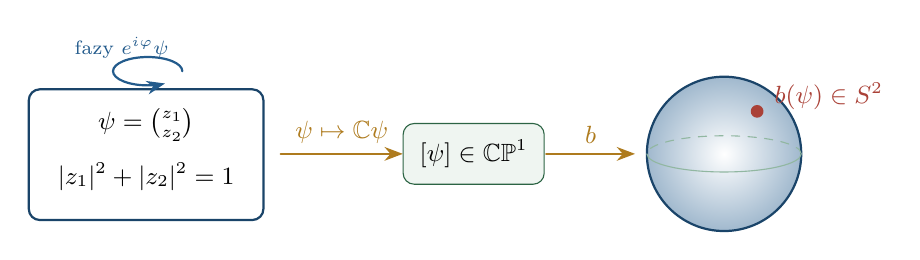
\begin{tikzpicture}[>=Stealth,line cap=round,scale=1.0]
 \draw[manifoldblue!75!black,thick,rounded corners]
 (-5.6,-.72) rectangle (-2.62,.94);
 \node[font=\small] at (-4.11,.49)
   {$\psi=\binom{z_1}{z_2}$};
 \node[font=\small] at (-4.11,-.17)
   {$|z_1|^2+|z_2|^2=1$};
 \draw[->,manifoldblue,thick] (-3.65,1.17)
  arc[start angle=0,end angle=300,x radius=.44,y radius=.18];
 \node[font=\scriptsize,manifoldblue] at (-4.42,1.47)
  {fazy $e^{i\varphi}\psi$};
 \draw[->,thick,manifoldgold!85!black] (-2.4,.12)--(-.85,.12)
  node[midway,above,font=\small] {$\psi\mapsto\C\psi$};
 \node[draw=manifoldgreen!80!black,rounded corners,
  fill=manifoldgreen!8,font=\small,inner sep=6pt] at (.05,.12)
  {$[\psi]\in\mathbb{CP}^1$};
 \draw[->,thick,manifoldgold!85!black] (.97,.12)--(2.1,.12)
  node[midway,above,font=\small] {$b$};
 \shade[inner color=white,outer color=manifoldblue!43] (3.23,.12) circle (.98);
 \draw[manifoldblue!75!black,thick] (3.23,.12) circle (.98);
 \draw[manifoldgreen!55,thin] (2.25,.12)
   arc[start angle=180,end angle=360,x radius=.98,y radius=.23];
 \draw[manifoldgreen!55,thin,dashed] (4.21,.12)
   arc[start angle=0,end angle=180,x radius=.98,y radius=.23];
 \fill[manifoldred] (3.65,.66) circle (2.3pt);
 \node[manifoldred,font=\small] at (4.56,.85) {$b(\psi)\in S^2$};
\end{tikzpicture}
\caption{Spinor jednostkowy $\psi\in\C^2$ ma fazę,
która nie zmienia prostej $[\psi]\in\mathbb{CP}^1$.
Wzór~\eqref{eq:spin-bloch} przypisuje tej prostej
punkt sfery. To łączy spinory z grassmannianem prostych.}
\label{fig:spin-bloch}
\end{figure}

\section{Struktury spinowe i wiązki spinorów}
\label{sec:struktura-spinowa}

Dotąd wektory, obroty i spinory należały do jednej
ustalonej przestrzeni $\R^n$. Na rozmaitości
przestrzeń $T_pM$ zmienia się z $p$.
Gładka rodzina dodatnio określonych iloczynów
skalarnych $g_p$ na $T_pM$ to \emph{metryka
riemannowska}. Pozwala wybierać bazy ortonormalne
w każdym punkcie. Jeśli $M$ jest zorientowana,
możemy wybierać bazy o dodatniej orientacji.

\emph{Wiązka dodatnio zorientowanych ramek
ortonormalnych} $F^+(M)\to M$ ma w punkcie $p$
za włókno wszystkie uporządkowane bazy
$(u_1,\ldots,u_n)$ przestrzeni $T_pM$,
które są ortonormalne i dodatnie.
Grupa $\mathrm{SO}(n)$ działa z prawej strony
przez zmianę takiej bazy. Nie ma wyróżnionej
bazy w każdym włóknie; lokalnie wiązka wygląda
jednak jak $U\times\mathrm{SO}(n)$.
Wiązkę o takiej lokalnej postaci, z wolnym
działaniem grupy przechodzącym tranzytywnie
na każdym włóknie, nazywamy \emph{wiązką główną}.

\begin{definicja}[Struktura spinowa i wiązka spinorów]
\index{struktura spinowa i wiazka spinorow@Struktura spinowa i wiązka spinorów}
\label{def:struktura-spinowa}
Dla zorientowanej rozmaitości riemannowskiej
$M^n$, $n\geq2$, \emph{struktura spinowa}
składa się z wiązki głównej
$P_{\mathrm{Spin}}\to M$ o grupie
$\operatorname{Spin}(n)$ oraz odwzorowania
gładkiego $\lambda:P_{\mathrm{Spin}}\to F^+(M)$
nad identycznością bazy, takiego że
\[
 \lambda(pg)=\lambda(p)\rho(g),
 \qquad g\in\operatorname{Spin}(n),
\]
a $\lambda$ ograniczona do każdego włókna
jest dwukrotnym nakryciem.
\emph{Wiązka spinorów} to wiązka zespolona
\[
 S:=P_{\mathrm{Spin}}\times_{\operatorname{Spin}(n)}\Delta_n.
\]
Jej elementami są klasy par $(p,\psi)$,
$p\in P_{\mathrm{Spin}}$, $\psi\in\Delta_n$,
z relacją $(pg,\psi)\sim(p,c(g)\psi)$.
\emph{Polem spinorowym} nazywamy gładki przekrój $S$.
Tę samą definicję stosujemy do dowolnej zorientowanej wiązki
euklidesowej $E$ rzędu $n$, zastępując $F^+(M)$ wiązką jej
dodatnich ramek ortonormalnych $F^+(E)$.
\end{definicja}

Po wyborze lokalnej ramki spinowej $s_i:U_i\to P_{\mathrm{Spin}}$
wiązka $S$ wygląda jak $U_i\times\Delta_n$. Ustalmy kierunek
zmian: jeśli $s_j=s_i h_{ij}$, to
$[s_j,\psi_j]=[s_i,c(h_{ij})\psi_j]$, zatem współrzędne
tego samego spinora spełniają $\psi_i=c(h_{ij})\psi_j$.
Przy przejściu od kolumny $i$ do kolumny $j$ używamy więc
macierzy odwrotnej. Z równości dla lokalnych ramek wynika też
$h_{ij}h_{jk}=h_{ik}$; reprezentacja $c$ przenosi tę równość
na macierze przejścia, co uzasadnia strukturę wiązki wektorowej $S$.
Zauważmy też, że $\lambda$ jest nakryciem całych przestrzeni:
w lokalnej trywializacji zadanej przez $s_i$ i ramkę $\lambda\circ s_i$
ma postać $(x,g)\mapsto(x,\rho(g))$.
Jeśli zmiana ramki wektorowej wykonuje pełny
obrót o $2\pi$, jej podniesienie w Spin
może dojść do $-1$. Wtedy wektory wracają
do wartości początkowych, lecz spinor dostaje
znak minus. To lokalna treść różnicy między
wiązką wektorów i wiązką spinorów.

\begin{przyklad}[Płaszczyzna i sfera są spinowe]
Na $\R^n$ standardowe ramki dają
$F^+(\R^n)\cong\R^n\times\mathrm{SO}(n)$.
Bierzemy
$P_{\mathrm{Spin}}=\R^n\times\operatorname{Spin}(n)$
i $\lambda(x,s)=(x,\rho(s))$; spinory
tworzą trywialną wiązkę
$S\cong\R^n\times\Delta_n$.

Na sferze $S^2\subset\R^3$ każda dodatnia
ramka styczna $(u,v)$ w punkcie $p$ wyznacza
macierz o kolumnach $(u,v,p)\in\mathrm{SO}(3)$.
To utożsamia $F^+(S^2)$ z $\mathrm{SO}(3)$,
a rzut do bazy wysyła macierz na jej trzecią
kolumnę $p$. Dwukrotne nakrycie
$\mathrm{SU}(2)\cong\operatorname{Spin}(3)
\to\mathrm{SO}(3)$ z
Przykładu~\ref{prz:spin3} daje odwzorowanie $\lambda$.
Rzut z $\operatorname{Spin}(3)$ do sfery ma postać
$q(s)=\rho(s)e_3$. Używamy jednej, ustalonej podgrupy
$H=\rho^{-1}(\operatorname{Stab}(e_3))=\operatorname{Spin}(2)$,
złożonej z $\cos t+\sin t\,e_1e_2$. Działa ona z prawej strony
na $\operatorname{Spin}(3)$ i zachowuje $q(s)$.
Jeśli $q(s)=q(s')$, to $s^{-1}s'\in H$, więc działanie jest
wolne i przechodnie na każdym włóknie. Lokalne gładkie ramki
styczne $(u,v)$ dają lokalne sekcje w $\mathrm{SO}(3)$;
po zmniejszeniu otoczenia podnosimy je przez lokalną odwrotność
nakrycia $\rho$. To zapewnia lokalną trywialność wiązki głównej.
Równość $\lambda(sh)=\lambda(s)\rho(h)$ kończy sprawdzenie
definicji struktury spinowej na sferze.
\end{przyklad}

\begin{uwaga}[Podnoszenie na zbiorze ściągalnym]
\label{rem:spin-podnoszenie}
Użyjemy elementarnego faktu o nakryciach: gładkie odwzorowanie
ze ściągalnego obszaru $U$ do podstawy gładkiego nakrycia ma
gładkie podniesienie po wybraniu obrazu jednego punktu.
Istotnie, drogę od tego punktu podnosimy kolejno przez lokalne
odwrotności nakrycia, dzieląc jej przedział parametrów na skończenie
wiele odcinków. Jednoznaczność na przecięciach daje jednoznaczność
podniesionej drogi. Homotopię dróg o ustalonych końcach podnosimy
analogicznie po podziale kwadratu parametrów na małe prostokąty,
których obrazy leżą w dziedzinach lokalnych odwrotności.
Końcowy punkt podniesienia nie zmienia się w tej homotopii:
poruszałby się ciągle w dyskretnym włóknie. W obszarze ściągalnym
każde dwie drogi o tych samych końcach są tak homotopijne,
więc ich podniesienia wyznaczają tę samą wartość w punkcie końcowym.
Otrzymana funkcja jest lokalnie złożeniem danej funkcji z jedną
lokalną odwrotnością nakrycia, zatem jest gładka.
Ten sam argument działa na dysku z brzegiem.
\end{uwaga}

\begin{przyklad}[Wiązka, której nie da się podnieść]
\label{prz:nie-spin-linia}
Podłoże $S^2\cong\mathbb{CP}^1$ jest spinowe,
ale nie każda \emph{wiązka} nad nim dopuszcza
podniesienie struktury do Spin.
Weźmy zespoloną wiązkę tautologiczną
$\gamma^1_\C$ nad
$\operatorname{Gr}_1(\C^2)=\mathbb{CP}^1$
i potraktujmy jej włókna jako rzeczywiste
zorientowane płaszczyzny wymiaru $2$.
Na mapie $[1:z]$ mamy ramkę zespoloną
$s_0(z)=(1,z)$, a na mapie $[w:1]$,
$w=1/z$, ramkę $s_\infty(w)=(w,1)$.
Na przecięciu
$s_\infty(1/z)=z^{-1}s_0(z)$.
Po unormowaniu ramek, przy $|z|=1$, $z=e^{i\theta}$, unitarny
czynnik przejścia jest więc $e^{-i\theta}$:
jako rzeczywista izometria obraca płaszczyznę
o kąt $-\theta$. Po przejściu
$0\leq\theta\leq2\pi$ daje pętlę
o nieparzystej liczbie pełnych obrotów.
Ta pętla w $\mathrm{SO}(2)$ nie ma
\emph{zamkniętego} podniesienia do $\operatorname{Spin}(2)$:
połowa kąta biegnie
od $0$ do $-\pi$ i kończy w $-1$, nie w $1$.
Gdyby istniała struktura spinowa, ramkę ortonormalną nad każdą
z dwóch półkul można by podnieść do ramki spinowej.
Rzeczywiście, przeciwobraz takiej ramki przez $\lambda$ jest
dwukrotnym nakryciem dysku; Uwagi~\ref{rem:spin-podnoszenie}
używamy do podniesienia identyczności dysku. Przejście między
otrzymanymi ramkami spinowymi na równiku byłoby właśnie
zamkniętym podniesieniem opisanej pętli, co jest sprzecznością.
Zmiana ramki na którejś z dwóch półkul
zmienia pętlę tylko o taką, która przedłuża
się na dysk i ma zerowy całkowity obrót.
Dlatego ten brak podniesienia nie zależy
od wybranych ramek. Wiązka rzeczywista otrzymana przez zapomnienie
struktury zespolonej $\gamma^1_\C$ nie ma struktury
spinowej, mimo że sama sfera $S^2$ ją ma.
\end{przyklad}

\begin{stwierdzenie}[Znaki na potrójnych przecięciach]
\label{prop:w2-znaki}
Niech $E$ będzie zorientowaną wiązką euklidesową
rzędu $n\geq2$ nad $M$. Weźmy dostatecznie drobne
pokrycie trywializujące $(U_i)$, w którym
niepuste skończone przecięcia są ściągalne. Takie pokrycie
nazywamy \emph{dobrym}; w tym stwierdzeniu zakładamy jego wybór.
Niech $g_{ij}:U_i\cap U_j\to\mathrm{SO}(n)$
przepisują współrzędne z trywializacji $j$ do trywializacji $i$,
więc $g_{ij}g_{jk}=g_{ik}$.
Na przecięciach wybierzmy podniesienia
$h_{ij}:U_i\cap U_j\to\operatorname{Spin}(n)$
z $\rho(h_{ij})=g_{ij}$ i $h_{ji}=h_{ij}^{-1}$.
Wtedy na potrójnym przecięciu
\begin{equation}\label{eq:w2-znaki}
 \varepsilon_{ijk}:=h_{ij}h_{jk}h_{ki}
          \in\{1,-1\}.
\end{equation}
Wiązka $E$ ma strukturę spinową dokładnie wtedy,
gdy wybory $h_{ij}$ można zmodyfikować znakami
tak, aby wszystkie $\varepsilon_{ijk}$ wynosiły $1$.
\end{stwierdzenie}
\begin{proof}
Z warunku kocyklu dla $g_{ij}$ mamy
$\rho(\varepsilon_{ijk})
=g_{ij}g_{jk}g_{ki}=I$.
Twierdzenie~\ref{thm:spin-nakrycie} mówi, że
jądro $\rho$ to $\{\pm1\}$; ponieważ znak jest
dyskretny, $\varepsilon_{ijk}$ jest lokalnie stały.
Nie ma problemu z samym podniesieniem
$g_{ij}$ na ściągalnym przecięciu:
zapewnia je Uwaga~\ref{rem:spin-podnoszenie}.
Przyjmujemy też $h_{ii}=1$.

Jeżeli na każdym potrójnym przecięciu
$\varepsilon_{ijk}=1$, to
$h_{ij}h_{jk}=h_{ik}$.
Są to funkcje przejścia z warunkiem kocyklu.
Sklejamy $U_i\times\operatorname{Spin}(n)$ relacją
$(x,a)_j\sim(x,h_{ij}(x)a)_i$. Warunek kocyklu zapewnia
przechodniość tej relacji, a gładkie przejścia zapewniają lokalne
trywializacje, jak w Sekcji~\ref{sec:wiazki-wektorowe}.
Działanie z prawej strony jest dobrze określone, wolne
i przechodnie we włóknach, więc otrzymujemy wiązkę główną.
Jeśli $f_i$ oznacza wybraną lokalną ramkę $E$, to
$\lambda([x,a]_i)=f_i(x)\rho(a)$ jest niezależne od reprezentanta,
ponieważ $f_j=f_i g_{ij}$ i $\rho(h_{ij})=g_{ij}$.
Lokalnie jest to $\id\times\rho$, a więc spełnia definicję
struktury spinowej.
Odwrotnie, w istniejącej strukturze spinowej podnosimy każdą
ustaloną ramkę $f_i$ do ramki spinowej nad ściągalnym $U_i$.
Stosujemy Uwagę~\ref{rem:spin-podnoszenie} do dwukrotnego
nakrycia będącego przeciwobrazem $f_i$ przez $\lambda$.
Przejścia tych ramek podnoszą właśnie dane $g_{ij}$ i spełniają
warunek kocyklu, więc wszystkie znaki są $1$.
Dowolne dwa odwzorowania $h_{ij}$ nad
tym samym $g_{ij}$ różnią się na spójnym
przecięciu stałym znakiem
$\delta_{ij}\in\{\pm1\}$.
Zmiana podniesień zastępuje
$\varepsilon_{ijk}$ przez
$\delta_{ij}\delta_{jk}\delta_{ki}
\varepsilon_{ijk}$, co dowodzi
sformułowania o modyfikacji znakami.
\end{proof}

\begin{uwaga}[Druga klasa Stiefela--Whitneya]
Zdarza się, że pojedynczych znaków
$\varepsilon_{ijk}$ nie da się wszystkich
usunąć. Ich układ spełnia warunek zgodności
na poczwórnych przecięciach: dwa sposoby
pomnożenia $h_{ij}h_{jk}h_{k\ell}$
dają
$\varepsilon_{ijk}\varepsilon_{ik\ell}
=\varepsilon_{jk\ell}\varepsilon_{ij\ell}$.
Taką rodzinę znaków nazywamy
\emph{dwukocyklowym} zapisem przeszkody.
Zmiany przez $\delta_{ij}$ z dowodu
uznajemy za równoważne. Nie zmienia tego wybór lokalnych ramek:
jeśli $f'_i=f_i a_i$, wybieramy podniesienia $b_i$ funkcji $a_i$
nad ściągalnymi $U_i$. Wtedy $g'_{ij}=a_i^{-1}g_{ij}a_j$
mają podniesienia $h'_{ij}=b_i^{-1}h_{ij}b_j$.
Ich iloczyn na potrójnym przecięciu to
$b_i^{-1}\varepsilon_{ijk}b_i=\varepsilon_{ijk}$,
bo znaki należą do centrum grupy Spin.
Klasa tego układu w
$H^2(M;\Z/2)$ nazywa się
\emph{drugą klasą Stiefela--Whitneya}
$w_2(E)$. Na dobrym pokryciu
$w_2(E)=0$ oznacza dokładnie, że znaki
można usunąć, czyli że struktura spinowa
istnieje. Identyfikacja klas z różnych
pokryć to twierdzenie kohomologii Čech;
używamy tu tylko elementarnego testu
podnoszenia funkcji przejścia dowiedzionego
wyżej. Dla wiązki w
Przykładzie~\ref{prz:nie-spin-linia}
przeszkoda jest niezerowa.
\end{uwaga}

\par\smallskip
{\footnotesize\noindent\emph{Dalsza lektura:}
Rachunki z konwencją $v^2=-\|v\|^2$
można porównać z notatkami Briana Conrada,
\emph{Clifford algebras and spin groups},
\url{https://math.stanford.edu/~conrad/210CPage/handouts/clifford.pdf}.
Budowę struktur spinowych i opis przeszkody
$w_2$ rozwijają notatki Konstantina Wernliego,
\emph{Lecture Notes on Spin Geometry},
\url{https://arxiv.org/pdf/1911.09766}.
Obie lektury używają miejscami innej kolejności tematów.
Powyższy test znaków został dowiedziony bez użycia kohomologii;
jego interpretacja jako klasy w $H^2$ korzysta z teorii
kohomologii Čech, której tutaj nie dowodziliśmy.\par}
\clearpage

\chapter{Podstawy algebry abstrakcyjnej}
\label{ch:algebra-abstrakcyjna}
\index{algebra abstrakcyjna@Algebra abstrakcyjna}

Zbierzemy pojęcia grup, pierścieni i modułów potrzebne
do algebry homologicznej. Konstrukcje ilorazowe pozwalają
narzucać relacje, a iloczyn tensorowy pozwala zastąpić
odwzorowanie dwuliniowe liniowym. Wcześniejszy
Rozdział~\ref{ch:algebra-tensorowa} dotyczył przestrzeni
nad ciałem; tutaj pracujemy nad pierścieniem.
W Rozdziale~\ref{ch:grass-spin} wystąpił też moduł
algebry Clifforda; wrócimy do tego przykładu.

\section{Grupy, słowa i prezentacje}
\label{sec:grupy-prezentacje-5}
\index{grupa wolna@Grupa wolna}
\index{prezentacja grupy@Prezentacja grupy}

Zanim przejdziemy do modułów, zbierzmy język
potrzebny przy grupie podstawowej i
Twierdzeniu~\ref{thm:van-kampen}. Grupa opisuje
odwracalne składanie działań. W grupie klas
pętli opartych w jednym punkcie działaniem
jest składanie pętli, a odwrotność reprezentuje
pętla przebiegnięta w przeciwnym kierunku.

\begin{definicja}[Grupa i homomorfizm]
\index{grupa i homomorfizm@Grupa i homomorfizm}
\label{def:grupa-hom-5}
\emph{Grupa} $(G,\cdot,1)$ to zbiór z łącznym
mnożeniem, elementem neutralnym $1$ i
odwrotnością $g^{-1}$ każdego $g\in G$.
Nie zakładamy przemienności. Odwzorowanie
$\varphi:G\to H$ jest \emph{homomorfizmem},
jeśli $\varphi(gh)=\varphi(g)\varphi(h)$.
Wtedy $\varphi(1)=1$ i
$\varphi(g^{-1})=\varphi(g)^{-1}$.
\end{definicja}

Przykładem jest $(\Z,+,0)$;
w zapisie addytywnym odwrotnością $m$
jest $-m$. Grupa permutacji trzech
elementów dostarcza przykładu
nieprzemiennego: przestawienia
$(12)(23)$ i $(23)(12)$ są różne.

\begin{definicja}[Podgrupa normalna i iloraz]
\index{podgrupa normalna i iloraz@Podgrupa normalna i iloraz}
\label{def:normal-quotient-5}
Podgrupa $N\leq G$ jest \emph{normalna},
gdy $gNg^{-1}=N$ dla każdego $g\in G$.
Wówczas zbiór warstw $G/N$ staje się
grupą przez $(gN)(hN)=ghN$.
Jądro homomorfizmu
$\ker\varphi=\{g:\varphi(g)=1\}$
jest normalne. \emph{Domknięcie normalne}
zbioru $R\subset G$, oznaczane
$\langle\!\langle R\rangle\!\rangle$,
jest najmniejszą podgrupą normalną
zawierającą $R$.
\end{definicja}

\begin{proof}[Dlaczego iloraz jest dobrze określony?]
Jeśli $g'=gn$ i $h'=hm$ dla $n,m\in N$,
to $g'h'=gnhm=gh(h^{-1}nh)m$.
Normalność daje $h^{-1}nh\in N$,
zatem $g'h'N=ghN$. Mnożenie
nie zależy więc od wybranych
reprezentantów. Dla jądra:
$\varphi(gng^{-1})=
\varphi(g)1\varphi(g)^{-1}=1$.
Elementy domknięcia normalnego
są skończonymi iloczynami
sprzężeń $grg^{-1}$ i ich
odwrotności, $r\in R$:
zbiór tych iloczynów jest
podgrupą normalną zawierającą
$R$ i mieści się w każdej takiej
podgrupie.
\end{proof}

\begin{przyklad}[Reszty modulo $m$]
\label{prz:Zmodm-grupa-5}
Niech $m\geq2$.
W grupie addytywnej $\Z$ każda
podgrupa jest normalna.
Iloraz $\Z/m\Z$ ma elementy
$[0],\ldots,[m-1]$ i dodawanie
$[a]+[b]=[a+b]$. Homomorfizm
$\Z\to\Z/m\Z$ ma jądro $m\Z$.
\end{przyklad}

\begin{definicja}[Grupa wolna i iloczyn wolny]
\index{grupa wolna i iloczyn wolny@Grupa wolna i iloczyn wolny}
\index{slowo w grupie wolnej@słowo w grupie wolnej}
\label{def:free-groups-5}
Niech $A$ będzie zbiorem \emph{symboli},
zwanych generatorami. Dla każdego $a\in A$
tworzymy nowy symbol $a^{-1}$;
zbiór tych nowych symboli oznaczamy $A^{-1}$
i przyjmujemy $(a^{-1})^{-1}=a$.
\emph{Słowo} w alfabecie
$A^{\pm1}=A\sqcup A^{-1}$ jest skończonym
ciągiem liter $x_1\cdots x_r$, $r\geq0$.
Długość słowa to $r$; jedyne słowo długości
zero oznaczamy $\varnothing$ i nazywamy pustym.
Słowa można sklejać, czyli konkatenować:
$(x_1\cdots x_r)(y_1\cdots y_s)
=x_1\cdots x_ry_1\cdots y_s$.

\emph{Redukcja elementarna} usuwa sąsiednie
litery $xx^{-1}$ lub $x^{-1}x$.
Słowo jest \emph{zredukowane}, gdy nie zawiera
takiej pary. Dwa słowa uznajemy za równoważne,
jeżeli można przejść od jednego do drugiego
skończonym ciągiem wstawień lub usunięć
takich par. \emph{Grupa wolna} $F(A)$
to zbiór tych klas, z mnożeniem zadanym
przez sklejanie słów.

Dla grup $G,H$ \emph{iloczyn wolny} $G*H$
powstaje analogicznie ze słów o literach
z $G\setminus\{1_G\}$ i $H\setminus\{1_H\}$.
Redukcja mnoży sąsiednie litery pochodzące
z tego samego czynnika i usuwa otrzymaną
jedynkę. Słowo zredukowane ma litery
z $G$ i $H$ naprzemiennie.
\end{definicja}

Zanim utożsamimy klasy ze słowami zredukowanymi,
trzeba wiedzieć, że wynik redukcji nie zależy
od kolejności kasowania par. Sam zbiór
\emph{wszystkich} słów z konkatenacją
jest tylko monoidem: słowa $aa^{-1}$
i $\varnothing$ nie są w nim dosłownie równe.

\begin{stwierdzenie}[Jednoznaczna postać zredukowana]
\index{redukcja slowa@redukcja słowa}
\label{prop:free-reduction-5}
Każda klasa w $F(A)$ zawiera dokładnie jedno
słowo zredukowane. Jeżeli $\operatorname{red}(w)$
oznacza to słowo, działanie grupowe ma postać
\[
 u\cdot v=\operatorname{red}(uv),\qquad
 1=\varnothing,\qquad
 (x_1\cdots x_r)^{-1}=x_r^{-1}\cdots x_1^{-1}.
\]
\end{stwierdzenie}
\begin{proof}
Czytamy słowo od lewej do prawej i trzymamy
\emph{stos} już przeczytanych liter.
Gdy następna litera jest odwrotnością
litery na wierzchu stosu, zdejmujemy wierzch;
w przeciwnym razie dokładamy nową literę.
Po ostatnim kroku na stosie nie ma sąsiedniej
pary odwrotnej, więc otrzymaliśmy słowo
zredukowane.

Sprawdźmy niezależność od usuwania par.
Operacja dopisania litery $x$ do słowa
na stosie jest odwracalna: operacja
dopisania $x^{-1}$ cofa ją, zarówno gdy
pierwszy krok dołożył literę, jak i wtedy,
gdy ją skasował. Dlatego przeczytanie
fragmentu $xx^{-1}$ nie zmienia stanu stosu.
Usunięcie takiego fragmentu z dowolnego miejsca
słowa nie zmienia końcowego wyniku algorytmu.
Każde słowo równoważne daje zatem ten sam wynik.
Jeśli słowo jest już zredukowane, algorytm
pozostawia je bez zmian; w każdej klasie
może więc być tylko jedno takie słowo.

Sklejanie jest łączne przed redukcją, a
usuwanie par nie zmienia wyniku algorytmu.
Stąd $\operatorname{red}(\operatorname{red}(uv)w)
=\operatorname{red}(uvw)
=\operatorname{red}(u\operatorname{red}(vw))$.
Słowo puste jest jedynką. Zapisane w tezie
słowo odwrotne po sklejeniu z oryginałem
redukuje się kolejno od środka do słowa pustego.
To sprawdza wszystkie aksjomaty grupy.
\end{proof}

\begin{przyklad}[Słowa i działanie na słowach]
\label{prz:redukcja-slow-5}
W $F(\{a,b\})$ słowo
$ab\,b^{-1}a^{-1}ba$
redukujemy najpierw do
$aa^{-1}ba$, a następnie
do $ba$. Słowa $ab$ i $ba$
są już zredukowane i różne,
więc grupa ta nie jest przemienna.
Dla jednego generatora każde słowo
redukuje się do $a^m$ z jednoznacznym
$m\in\Z$; stąd $F(\{a\})\cong\Z$.

Grupa $F(A)$ działa na zbiorze zredukowanych
słów przez mnożenie z lewej:
$u\cdot w=\operatorname{red}(uw)$.
Na przykład $a\cdot(a^{-1}b)=b$.
Jest to działanie, bo łączność udowodniono
powyżej; odwrotna operacja do działania
przez $a$ to działanie przez $a^{-1}$.
Jest ono przechodnie, gdyż $w\cdot\varnothing=w$,
i wolne: jeśli $u\cdot w=w$, to w grupie
$uw=w$, zatem po pomnożeniu przez $w^{-1}$
dostajemy $u=1$. Ten sam zbiór ma również
działanie z prawej $w\cdot u=\operatorname{red}(wu)$.
Rysunek~\ref{fig:free-words-5} pokazuje
pojedyncze kroki tego drugiego działania.
Na przykład iloczyn dwóch zredukowanych słów
$ab$ i $b^{-1}a$ trzeba jeszcze skrócić:
$\operatorname{red}(ab\,b^{-1}a)=a^2$.
\end{przyklad}

\begin{figure}[htbp]
\centering
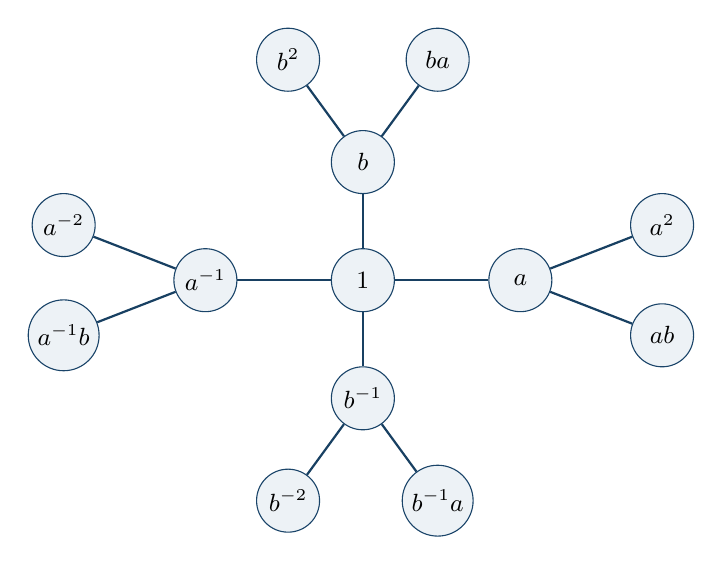
\begin{tikzpicture}[>=Latex,font=\small,
 every node/.style={circle,draw=manifoldblue!75!black,
 fill=manifoldblue!8,inner sep=2pt,minimum size=8mm}]
 \node (e) at (0,0) {$1$};
 \node (a) at (2,0) {$a$};
 \node (ai) at (-2,0) {$a^{-1}$};
 \node (b) at (0,1.5) {$b$};
 \node (bi) at (0,-1.5) {$b^{-1}$};
 \node (aa) at (3.8,.7) {$a^2$};
 \node (ab) at (3.8,-.7) {$ab$};
 \node (aiai) at (-3.8,.7) {$a^{-2}$};
 \node (aib) at (-3.8,-.7) {$a^{-1}b$};
 \node (bb) at (-.95,2.8) {$b^2$};
 \node (ba) at (.95,2.8) {$ba$};
 \node (bibi) at (-.95,-2.8) {$b^{-2}$};
 \node (bia) at (.95,-2.8) {$b^{-1}a$};
 \foreach \x/\y in {e/a,e/ai,e/b,e/bi,a/aa,a/ab,
 ai/aiai,ai/aib,b/bb,b/ba,bi/bibi,bi/bia}
   \draw[thick,manifoldblue!70!black] (\x)--(\y);
\end{tikzpicture}
\caption{Fragment grafu słów zredukowanych w
$F(\{a,b\})$. Krawędź oznacza dopisanie
z prawej jednej litery $a^{\pm1}$ albo $b^{\pm1}$
i ewentualną redukcję. Powrót po krawędzi
odpowiada dopisaniu litery odwrotnej.}
\label{fig:free-words-5}
\end{figure}

\begin{stwierdzenie}[Własność uniwersalna grupy wolnej]
\label{prop:free-universal-5}
Dla dowolnej grupy $K$ i dowolnego wyboru
elementów $h_a\in K$, $a\in A$, istnieje
dokładnie jeden homomorfizm $\Phi:F(A)\to K$
spełniający $\Phi(a)=h_a$.
\end{stwierdzenie}
\begin{proof}
Na słowach musi on mieć postać
\[
 \Phi(a_1^{\epsilon_1}\cdots a_r^{\epsilon_r})
 =h_{a_1}^{\epsilon_1}\cdots h_{a_r}^{\epsilon_r},
 \qquad \epsilon_i\in\{1,-1\}.
\]
Usunięcie sąsiedniej pary odwrotnej nie zmienia
iloczynu po prawej. Wzór zależy więc tylko
od klasy słowa i jest dobrze określony.
Sklejanie słów odpowiada mnożeniu obrazów,
zatem $\Phi$ jest homomorfizmem.
Każde słowo jest iloczynem generatorów
i ich odwrotności, co dowodzi jednoznaczności.
Właśnie brak dodatkowych relacji między
generatorami nazywamy \emph{wolnością}.
\end{proof}

W iloczynie wolnym $G*H$ działa podobny algorytm:
czytamy litery po kolei i trzymamy stos
liter różnych od jedynki, pochodzących naprzemiennie
z obu czynników. Nową literę z innego czynnika
dokładamy na stos; z tego samego mnożymy z literą
na wierzchu. Gdy iloczyn jest jedynką, usuwamy
wierzch i odsłaniamy poprzednią literę.
Operacja dopisania $x$ ma odwrotność: dopisanie
$x^{-1}$ z tego samego czynnika. Zatem usunięcie
sąsiednich liter jednego czynnika i zastąpienie
ich iloczynem nie zmienia końcowego stanu stosu.
Słowo już naprzemienne algorytm pozostawia bez zmian,
więc każda klasa ma dokładnie jedno takie słowo.
Stąd homomorfizmy $G\to K$ i $H\to K$
przedłużają się jednoznacznie na $G*H$.
To jest własność używana później w
Twierdzeniu~\ref{thm:van-kampen}.

Na przykład dla $G=\langle a\rangle\cong\Z$
i $H=\langle b\rangle\cong\Z$ własności
uniwersalne dają $G*H\cong F(\{a,b\})$.
Iloczyn słów naprzemiennych
$(ab)(b^{-1}a)$ redukuje się do $a^2$:
po skasowaniu $bb^{-1}$ zostaje $aa$.

\begin{definicja}[Prezentacja grupy]
\index{prezentacja grupy@Prezentacja grupy}
\label{def:prezentacja-grupy-5}
Jeśli $R$ jest zbiorem słów
w $F(A)$, to
\[
 \langle A\mid R\rangle
 :=F(A)/\langle\!\langle R\rangle\!\rangle
\]
nazywamy \emph{grupą o generatorach}
$A$ i \emph{relacjach} $R$.
Relacja $r=1$ oznacza, że jej
wszystkie konsekwencje po
mnożeniu i sprzęganiu również
stają się jedynką.
\end{definicja}

\begin{przyklad}[Prezentacja grupy torusa]
\label{prz:prezentacja-torusa-5}
Niech $F(a,b)$ będzie grupą wolną
na dwóch symbolach. Relacja
$aba^{-1}b^{-1}=1$
jest równoważna $ab=ba$.
Po jej narzuceniu każde słowo
można przestawić do postaci
$a^m b^n$, $m,n\in\Z$.
Odwzorowanie
$F(a,b)\to\Z^2$ dane przez
$a\mapsto(1,0)$,
$b\mapsto(0,1)$
zabija tę relację i wysyła
$a^m b^n$ na $(m,n)$.
Postacie te są więc wzajemnie
różne, a zatem
\[
 \langle a,b\mid aba^{-1}b^{-1}\rangle
 \cong\Z^2.
\]
Sklejenie przeciwnych boków kwadratu
tworzy torus. Brzeg kwadratu przed
sklejeniem odczytujemy jako słowo
$aba^{-1}b^{-1}$.
Topologiczne uzasadnienie, że
prezentacja opisuje $\pi_1(T^2)$,
podamy przy
Twierdzeniu~\ref{thm:van-kampen}.
\end{przyklad}

\section{Pierścienie, ideały i ilorazy}
\label{sec:pierscienie-idealy}
\index{pierscien@Pierścień}
\index{ideal@Ideał}

W grupie normalność podgrupy pozwala utworzyć
iloraz. Dla pierścieni podobną rolę pełni ideał:
trzeba zachować nie tylko dodawanie, lecz także
mnożenie klas przez dowolne elementy pierścienia.

\begin{definicja}[Pierścień przemienny i homomorfizm]
\label{def:pierscien-przemienny}
\emph{Pierścień przemienny z jedynką} $R$ ma
dwa działania $+$ i mnożenie. Grupa $(R,+,0)$
jest abelowa, mnożenie jest łączne i przemienne,
ma jedynkę $1$, a rozdzielność
$r(s+t)=rs+rt$ wiąże oba działania.
Pierścień zerowy z $1=0$ jest dozwolony.
\emph{Homomorfizm pierścieni}
$\varphi:R\to S$ zachowuje dodawanie, mnożenie
i jedynkę: $\varphi(1_R)=1_S$.
\end{definicja}

Przykładami są $\Z$, $\Q$ i pierścień
wielomianów $\mathbb K[t]$ nad ciałem $\mathbb K$.
W $\Z$ nie każdy niezerowy element ma odwrotność
mnożeniową: równanie $2x=1$ nie ma rozwiązania
w $\Z$. To odróżnia pierścień od ciała.

\begin{definicja}[Ideał i pierścień ilorazowy]
\label{def:ideal-iloraz}
\emph{Ideał} $I\subseteq R$ jest podgrupą
addytywną zamkniętą na mnożenie przez
elementy $R$: jeśli $r\in R$ i $x\in I$,
to $rx\in I$. Pierścień $R/I$ ma klasy
$[r]=r+I$ oraz działania
$[r]+[s]=[r+s]$, $[r][s]=[rs]$.
\end{definicja}

\begin{proof}[Dlaczego iloraz jest dobrze określony?]
Jeżeli $r'=r+i$ i $s'=s+j$ dla $i,j\in I$,
to $r'+s'-(r+s)=i+j\in I$ oraz
$r's'-rs=rj+is+ij\in I$.
Dlatego wynik obu działań nie zależy od
wyboru przedstawicieli. Jądro homomorfizmu
$\varphi:R\to S$ jest ideałem: dla
$\varphi(x)=0$ mamy
$\varphi(rx)=\varphi(r)\varphi(x)=0$.
Gdy $I=R$, iloraz jest pierścieniem zerowym
z $[1]=[0]$.
\end{proof}

\begin{przyklad}[Dwie relacje w pierścieniach]
\label{prz:idealy-ilorazy}
Niech $m\geq2$. Ideał $m\Z$ narzuca
relację $m=0$, a iloraz $\Z/m\Z$ jest pierścieniem
reszt modulo $m$. W $\mathbb K[t]$
ideał $(t):=t\mathbb K[t]=
\{tf(t):f\in\mathbb K[t]\}$ składa się z wielomianów
o zerowym wyrazie stałym. Ewaluacja
$f(t)\mapsto f(0)$ ma jądro $(t)$,
a odwzorowanie $[f]\mapsto f(0)$
daje izomorfizm
$\mathbb K[t]/(t)\cong\mathbb K$.
Istotnie, każda klasa zawiera dokładnie
jedną stałą, bo $f(t)-f(0)$ jest podzielny
przez $t$.
\end{przyklad}

\section{Moduły, homomorfizmy i ilorazy}
\label{sec:moduly}

Przez $R$ oznaczamy pierścień przemienny z jedynką
$1\ne0$ w sensie Definicji~\ref{def:pierscien-przemienny}.
Pozwala to traktować wszystkie moduły
jednakowo, bez rozróżniania strony działania.
Wiele definicji działa również dla pierścieni
nieprzemiennych i modułów lewych; zaznaczymy,
gdzie przemienność upraszcza zapis.

\begin{definicja}[Moduł nad pierścieniem]
\index{modul nad pierscieniem@Moduł nad pierścieniem}
\label{def:modul}
\emph{Moduł $M$ nad $R$} to grupa abelowa
$(M,+,0)$ z mnożeniem przez skalary
$R\times M\to M$, $(r,m)\mapsto rm$, takim że
dla $r,s\in R$ i $m,n\in M$ mamy
\[
 (r+s)m=rm+sm,\qquad r(m+n)=rm+rn,\qquad
 (rs)m=r(sm),\qquad 1m=m.
\]
Grupa abelowa oznacza tutaj, że dodawanie w $M$
jest łączne, przemienne, ma element $0$ i każdy
element $m$ ma element przeciwny $-m$.
\end{definicja}

Definicja różni się od definicji przestrzeni liniowej
jedynie tym, że nie wymagamy dzielenia przez
niezerowy skalar. Ta różnica ma poważne skutki:
moduł może nie mieć bazy, a równanie $rm=0$ może
zachodzić dla $r\ne0$ i $m\ne0$.
W przypadku grup abelowych, czyli $\Z$-modułów,
opisujemy to precyzyjnie następująco.

\begin{definicja}[Element torsyjny i $m$-torsja]
\label{def:torsja}
Element $x$ grupy abelowej $M$ jest
\emph{torsyjny}, jeśli istnieje liczba całkowita
$k\ne0$ taka, że $kx=0$. Zbiór takich elementów
oznaczamy $\operatorname{Tors}(M)$ i nazywamy
\emph{podgrupą torsyjną}. Dla ustalonego $m\geq2$
definiujemy \emph{$m$-torsję}
\[
 M[m]:=\{x\in M:mx=0\}=\ker(\times m:M\to M).
\]
Podgrupa $M[m]$ składa się z elementów zabijanych
przez tę jedną liczbę $m$; cały
$\operatorname{Tors}(M)$ dopuszcza różne niezerowe
liczby dla różnych elementów.
\end{definicja}

Oba zbiory są rzeczywiście podgrupami: jeśli
$kx=0$ i $\ell y=0$, to $k\ell(x-y)=0$;
dla ustalonego $m$ mamy od razu
$m(x-y)=mx-my=0$. Na przykład
$\operatorname{Tors}(\Z\oplus\Z/2)
=0\oplus\Z/2$, podczas gdy $\Z$
nie ma niezerowej torsji.

\begin{przyklad}[Od grup abelowych do spinorów]
\label{prz:moduly-podstawowe}
\begin{enumerate}[leftmargin=*]
\item Każda przestrzeń liniowa nad ciałem
      $\mathbb K$ jest $\mathbb K$-modułem.
\item Każda grupa abelowa $A$ jest $\Z$-modułem:
      $na$ dla $n>0$ oznacza sumę $n$ kopii $a$,
      $0a=0$, a $(-n)a=-(na)$. Aksjomaty modułu
      wynikają z praw dodawania. Odwrotnie,
      w każdym $\Z$-module aksjomaty wymuszają
      właśnie tę regułę, więc pojęcia są równoważne.
\item Dla $m\geq2$ grupa $\Z/m\Z$ jest $\Z$-modułem;
      niezerowa klasa $[1]$ spełnia $m[1]=0$. Nie ma bazy
      nad $\Z$. Istotnie, gdyby $[1]=\sum_i a_i e_i$ w takiej
      bazie, równość $\sum_i ma_i e_i=0$ i jednoznaczność
      współczynników wymuszałyby $ma_i=0$ w $\Z$ dla każdego $i$.
      Stąd wszystkie $a_i=0$, sprzecznie z $[1]\ne0$.
\item $R/I$ dla ideału $I\subseteq R$ jest
      $R$-modułem: $r[s]=[rs]$. Działanie jest
      dobrze określone, gdyż z $s-s'\in I$
      wynika $r(s-s')\in I$.
\item Moduł spinorów z Definicji~\ref{def:spinor}
      jest modułem nad zespoloną algebrą
      Clifforda. Tam algebra może być
      nieprzemienna i działanie jest \emph{lewe};
      obecny rozdział używa pierścienia
      przemiennego, a zatem uogólnia ideę
      działania algebry w kierunku
      przydatnym dla grup homologii.
\end{enumerate}
\end{przyklad}

\begin{definicja}[Podmoduł, homomorfizm, moduł wolny]
\index{podmodul homomorfizm modul wolny@Podmoduł, homomorfizm, moduł wolny}
\label{def:modul-map}
Podzbiór $N\subseteq M$ jest \emph{podmodułem},
jeśli zawiera $0$ i jest zamknięty na dodawanie,
branie elementów przeciwnych i mnożenie przez $R$.
\emph{Homomorfizm} $f:M\to N$ spełnia
$f(m+m')=f(m)+f(m')$ oraz $f(rm)=rf(m)$.
Piszemy $\operatorname{Hom}_R(M,N)$
na zbiór takich odwzorowań; przy dodawaniu punktowym
i działaniu $(rf)(m)=r f(m)$ jest on
$R$-modułem. Tutaj wykorzystujemy przemienność $R$:
$(rf)(sm)=rsf(m)=s(rf)(m)$, więc mnożenie homomorfizmu
przez skalar zachowuje jego $R$-liniowość.

Moduł \emph{wolny} z bazą $(e_i)_{i\in I}$
ma tę własność, że każdy jego element jest
\emph{jednoznaczną skończoną} sumą
$\sum_{i\in I}r_i e_i$. Modelowym przykładem
jest $R^{(I)}$, zbiór rodzin $(r_i)$
o skończonym nośniku.
Sumę prostą $M\oplus N$ tworzą pary $(m,n)$ z działaniami
składowymi; jej naturalne włączenia to $m\mapsto(m,0)$
i $n\mapsto(0,n)$, a rzuty wybierają odpowiednią współrzędną.
\end{definicja}

Na przykład $\operatorname{Hom}_{\Z}(\Z/2,\Z)=0$:
homomorfizm jest wyznaczony przez obraz $[1]$, lecz
$2f([1])=f(2[1])=0$ wymusza $f([1])=0$ w $\Z$.

To jest ten sam sens \emph{formalnych kombinacji},
którego użyliśmy w Rozdziale~\ref{ch:algebra-tensorowa}:
poza aksjomatami nie narzucamy żadnych relacji
między symbolami $e_i$. W szczególności
$\Z^k$ jest wolnym $\Z$-modułem, ale
$\Z/m\Z$ przy $m>1$ nie jest wolny.

Jeśli $N\subseteq M$ jest podmodułem, to
\emph{moduł ilorazowy} $M/N$ składa się z klas
$[m]=m+N$. Dwie klasy są równe dokładnie wtedy,
gdy $m-m'\in N$. Działania
$[m]+[m']=[m+m']$ i $r[m]=[rm]$
nie zależą od reprezentantów: zmianę
$m\mapsto m+n$ i $m'\mapsto m'+n'$
pochłania zamknięcie $N$ na $n+n'$ i $rn$.

\begin{twierdzenie}[Pierwsze twierdzenie o izomorfizmie]
\label{thm:modul-izomorfizm}
Dla homomorfizmu $f:M\to N$ jądro
$\ker f=\{m:f(m)=0\}$ i obraz
$\operatorname{im}f=\{f(m):m\in M\}$
są podmodułami, a wzór
\[
 \overline f:M/\ker f\longrightarrow\operatorname{im}f,
 \qquad [m]\longmapsto f(m)
\]
jest izomorfizmem $R$-modułów.
\end{twierdzenie}
\begin{proof}
Jeśli $f(m)=f(m')=0$, to
$f(m-m')=0$ i $f(rm)=r f(m)=0$;
stąd jądro jest podmodułem. Jeżeli
$x=f(m)$ i $y=f(m')$, to
$x+y=f(m+m')$ i $rx=f(rm)$, więc
obraz także jest podmodułem.
Jeżeli $[m]=[m']$, to $m-m'\in\ker f$
i $f(m)-f(m')=0$; wzór na $\overline f$
nie zależy więc od przedstawiciela.
Jest liniowy dzięki liniowości $f$.
Jest surjektywny na obraz z jego definicji.
Gdy $\overline f([m])=0$, mamy
$m\in\ker f$, a zatem $[m]=[0]$.
Jądro $\overline f$ jest zerowe, więc
odwzorowanie jest również iniektywne.
\end{proof}

\section{Iloczyn tensorowy modułów}
\label{sec:tensor-modulow-algebra}
\index{iloczyn tensorowy modulow@Iloczyn tensorowy modułów}

W Rozdziale~\ref{ch:algebra-tensorowa} tensorowaliśmy
przestrzenie liniowe nad ciałem. Nad pierścieniem
budujemy podobny obiekt, lecz nie wolno już korzystać
z bazy dowolnego modułu. Intuicja pozostaje ta sama:
symbol $m\otimes n$ ma być liniowy w obu argumentach,
a każda zbiliniowa reguła na parach powinna przechodzić
przez jedno odwzorowanie liniowe.

\begin{definicja}[Iloczyn tensorowy modułów]
\label{def:tensor-modulow}
Niech $M,N$ będą $R$-modułami. Weźmy wolny
$R$-moduł $F=R^{(M\times N)}$ na formalnych
symbolach $[m,n]$. Niech $K\subseteq F$ będzie
podmodułem generowanym przez wszystkie elementy
\[
\begin{aligned}
 &[m+m',n]-[m,n]-[m',n],\\
 &[m,n+n']-[m,n]-[m,n'],\\
 &[rm,n]-r[m,n],\qquad [m,rn]-r[m,n],
\end{aligned}
\]
gdzie $m,m'\in M$, $n,n'\in N$ i $r\in R$.
\emph{Iloczyn tensorowy} to $M\otimes_R N=F/K$,
a $m\otimes n$ oznacza klasę $[m,n]+K$.
\end{definicja}

Podmoduł generowany przez relacje składa się
z ich \emph{skończonych} kombinacji $R$-liniowych.
To jest algebraiczny sens narzucenia relacji.
Ukończony iloczyn tensorowy jest innym pojęciem:
wymaga dodatkowej topologii lub normy na modułach
i nie występuje w tej konstrukcji.
Z definicji
$rm\otimes n=m\otimes rn=r(m\otimes n)$.
Każdy element jest skończoną sumą tensorów
prostych, lecz nie musi być jednym takim tensorem.

\begin{twierdzenie}[Własność uniwersalna tensoru]
\label{thm:tensor-modulow-uniwersalnosc}
Dla każdego $R$-modułu $P$ i każdego
odwzorowania $R$-dwuliniowego
$b:M\times N\to P$ istnieje dokładnie
jeden homomorfizm $\widetilde b:M\otimes_R N\to P$
spełniający $\widetilde b(m\otimes n)=b(m,n)$.
\end{twierdzenie}
\begin{proof}
Na wolnym module $F$ istnieje dokładnie
jeden homomorfizm $L:F\to P$ z
$L([m,n])=b(m,n)$: określamy go na bazie
i przedłużamy liniowo. Addytywność i
$R$-liniowość $b$ w każdej zmiennej oznaczają,
że $L$ zeruje cztery rodzaje generatorów $K$.
Stąd $K\subseteq\ker L$, więc wzór
$\widetilde b(x+K)=L(x)$ jest dobrze określony.
Tensory proste rozpinają iloraz $F/K$;
wartości na nich wymuszają jednoznaczność.
Ten sam argument, zastosowany w obie strony,
pokazuje, że każda inna realizacja tej własności
jest kanonicznie izomorficzna z $M\otimes_R N$.
\end{proof}

\begin{przyklad}[Jednostka i iloraz przez ideał]
\label{prz:tensor-jednostka-ideal}
Odwzorowanie $R\otimes_R M\to M$,
$r\otimes m\mapsto rm$, jest izomorfizmem;
jego odwrotność wysyła $m$ na $1\otimes m$.
Jeśli $I\subseteq R$ jest ideałem, połóżmy
$IM=\{\sum_{j=1}^q i_jm_j:
i_j\in I,\ m_j\in M\}$.
Wówczas
\begin{equation}\label{eq:tensor-ideal-iloraz}
 (R/I)\otimes_R M\cong M/IM,
 \qquad (r+I)\otimes m\longmapsto rm+IM.
\end{equation}
Istotnie, wzór jest dwuliniowy i nie zależy
od wyboru $r$, bo $i m\in IM$ dla $i\in I$.
Odwrotność wysyła $m+IM$ na
$(1+I)\otimes m$. Jeśli $i\in I$, to
$(1+I)\otimes im=(i+I)\otimes m=0$;
znika więc na całym $IM$. Oba złożenia
są identycznościami na generatorach.
Dla $R=\Z$ i $I=m\Z$ otrzymujemy
$(\Z/m)\otimes_{\Z}A\cong A/mA$.
\end{przyklad}

\begin{stwierdzenie}[Tensorowanie odwzorowań]
\label{prop:tensor-maps-algebra}
Homomorfizm $f:M\to M'$ indukuje
$f\otimes\id_N:M\otimes_R N\to M'\otimes_R N$
przez $(f\otimes\id_N)(m\otimes n)=f(m)\otimes n$.
Jeśli $f$ jest surjekcją, to $f\otimes\id_N$
jest surjekcją. Tensorowanie nie musi
zachowywać iniekcji.
\end{stwierdzenie}
\begin{proof}
Zbiliniowość pary $(m,n)\mapsto f(m)\otimes n$
i Twierdzenie~\ref{thm:tensor-modulow-uniwersalnosc}
dają indukowany homomorfizm.
Gdy $f$ jest surjekcją, każdy tensor prosty
$m'\otimes n$ ma przeciwobraz $m\otimes n$
z $f(m)=m'$. Tensory proste rozpinają cel,
więc indukowany homomorfizm jest surjekcją.
Dla iniekcji $f=\times2:\Z\to\Z$ oraz
$N=\Z/2$ identyfikacja
$\Z\otimes_{\Z}\Z/2\cong\Z/2$ pokazuje,
że $f\otimes\id_N$ jest odwzorowaniem zerowym:
$(2z)\otimes[1]=z\otimes[2]=0$.
Nie jest zatem iniekcją.
\end{proof}

\begin{definicja}[Rozszerzenie skalarów]
\label{def:rozszerzenie-skalarow}
Jeśli $\varphi:R\to S$ jest homomorfizmem
pierścieni przemiennych z jedynką, to $S$
staje się $R$-modułem przez $r\cdot s=\varphi(r)s$.
Na $M\otimes_R S$ działa $S$ przez
$s\cdot(m\otimes a)=m\otimes sa$.
Ten $S$-moduł nazywamy \emph{rozszerzeniem
skalarów} modułu $M$ wzdłuż $\varphi$.
\end{definicja}

Sprawdźmy relację zbalansowania dla działania
$S$: dla $r\in R$ oraz $s,a\in S$ mamy
\[
 s\cdot((rm)\otimes a)
 =m\otimes\varphi(r)sa
 =m\otimes s\varphi(r)a
 =s\cdot(m\otimes\varphi(r)a).
\]
Przemienność $S$ uzasadnia środkową równość;
relacje addytywności sprawdza się składnikowo.
Dlatego działanie nie zależy od zapisu elementu
jako sumy tensorów prostych. Dla wolnego
$M=\bigoplus_{i\in J}Re_i$ mamy
\[
 M\otimes_R S\cong\bigoplus_{i\in J}Se_i,
 \quad
 (\textstyle\sum_i r_i e_i)\otimes s
 \longmapsto\textstyle\sum_i\varphi(r_i)s e_i.
\]
Odwrotność wysyła $\sum_i s_i e_i$ na
$\sum_i e_i\otimes s_i$; wszystkie sumy są
skończone. Podobnie tensorowanie zachowuje
sumy proste i izomorfizmy, lecz powyższy
przykład z $\times2$ ostrzega przed
wnioskowaniem o dowolnych iniekcjach.

\begin{uwaga}[Moduły projektywne]
\label{uwaga:moduly-projektywne}
Moduł $P$ jest \emph{projektywny}, gdy dla każdej
surjekcji $q:E\twoheadrightarrow B$ i każdego
homomorfizmu $g:P\to B$ istnieje podniesienie
$\widetilde g:P\to E$ z $q\widetilde g=g$.
Równoważnie, $P$ jest składnikiem prostym
pewnego modułu wolnego. Jeśli $P$ jest projektywny,
wybieramy wolny moduł $F$ na symbolach elementów
$P$ i jego naturalną surjekcję $q:F\twoheadrightarrow P$.
Podnosimy $\id_P$ przez $q$; otrzymane rozszczepienie
daje $F\cong P\oplus\ker q$. Odwrotnie,
odwzorowanie z wolnego modułu można podnieść,
wybierając przeciwobrazy wartości na bazie.
Jeśli $F=P\oplus Q$, to dla $g:P\to B$
podnosimy $g\circ\operatorname{pr}_P:F\to B$
i ograniczamy otrzymane odwzorowanie do $P$.
Projektywny nie musi być wolny: dla
$R=\Z/6$ ideał $3R=\{0,3\}$ jest składnikiem
prostym w $R=3R\oplus4R$, lecz jego dwa
elementy wykluczają izomorfizm z $R^{(J)}$.
\end{uwaga}

W zastosowaniach do nieprzemiennego pierścienia
grupowego $\Z[\pi]$ rozróżnia się moduł prawy
i lewy. Wtedy tensor tworzy się z prawego
modułu $M$ i lewego $N$, narzucając relację
$(m\lambda)\otimes n=m\otimes(\lambda n)$.
Wersja projektywności przez podnoszenie i
składniki proste wolnych działa również tam.


\chapter{Algebra homologiczna: kompleksy i (ko)homologie}
\label{ch:algebra-homologiczna}
\index{homologia@Homologia}

Grupy, moduły i tensorowanie zebraliśmy w
Rozdziale~\ref{ch:algebra-abstrakcyjna}.
Teraz badamy ciągi odwzorowań między modułami.
W kompleksie łańcuchowym elementy spełniające
$\partial x=0$ są cyklami; część z nich ma postać
$x=\partial y$ i jest brzegami. Iloraz cykli
przez brzegi tworzy homologię. W kohomologii
strzałki biegną w przeciwną stronę.
Na razie prowadzimy rachunek algebraiczny;
później zastosujemy go do przestrzeni.

\section{Ciągi modułów i dokładność}
\label{sec:dokladnosc-modulow}

Mając kolejne homomorfizmy
\[
 \cdots\longrightarrow M_{i-1}
 \xrightarrow{f_{i-1}}M_i
 \xrightarrow{f_i}M_{i+1}
 \longrightarrow\cdots,
\]
pytamy, które elementy $M_i$ przychodzą z lewej
i które znikają po wysłaniu w prawo.
Samo słowo \emph{dokładny} odnosi się do
ciągu \emph{w danym miejscu}, a nie do
pojedynczego modułu.

\begin{definicja}[Dokładność ciągu]
\index{dokladnosc ciagu@Dokładność ciągu}
\label{def:ciag-dokladny}
Ciąg jest \emph{dokładny w $M_i$}, jeśli
\[
 \operatorname{im}f_{i-1}=\ker f_i.
\]
Jest \emph{dokładny}, jeśli tak jest
w każdym jego miejscu. Równość zawiera
dwa żądania: $f_i f_{i-1}=0$ oraz to,
że każdy element zabity przez $f_i$
już pochodzi z $M_{i-1}$.
\emph{Długi ciąg dokładny} ma wiele
następujących po sobie takich miejsc;
może rozciągać się w obie strony
bez wyznaczonego początku.
\end{definicja}

Ponieważ jedyne odwzorowanie $0\to M$ ma obraz $0$,
warunek dokładności $0\to A\xrightarrow{i}B$
w $A$ mówi $\ker i=0$, czyli $i$ jest iniekcją.
Analogicznie dokładność
$B\xrightarrow{p}C\to0$ w $C$ mówi
$\operatorname{im}p=C$, czyli $p$ jest surjekcją.

\begin{definicja}[Krótki ciąg dokładny]
\index{krotki ciag dokladny@Krótki ciąg dokładny}
\label{def:krotki-ciag}
Ciąg
\begin{equation}\label{eq:krotki-ciag}
 0\longrightarrow A\xrightarrow{i}B
   \xrightarrow{p}C\longrightarrow0
\end{equation}
jest \emph{krótki i dokładny}, gdy $i$ jest
iniekcją, $p$ jest surjekcją oraz
$\operatorname{im}i=\ker p$.
Wtedy $C\cong B/i(A)$ przez
Twierdzenie~\ref{thm:modul-izomorfizm}
zastosowane do $p$. Mówimy też,
że $B$ jest \emph{rozszerzeniem} $C$ przez $A$.
\end{definicja}

\begin{przyklad}[Reszty z dzielenia]
\label{prz:ses-mod-m}
Dla $m\geq2$ mamy krótki ciąg dokładny
\[
 0\longrightarrow\Z\xrightarrow{\ \times m\ }\Z
   \xrightarrow{\ \pi\ }\Z/m\Z\longrightarrow0,
 \qquad \pi(k)=[k].
\]
Pierwsze odwzorowanie jest iniektywne: $mk=0$
w $\Z$ pociąga $k=0$. Odwzorowanie $\pi$ jest
surjektywne, bo każda klasa ma reprezentanta.
Jej jądro to dokładnie wielokrotności $m$,
czyli obraz pierwszego odwzorowania.
\end{przyklad}

Krótki ciąg może, ale nie musi, rozkładać się
na dwie niezależne części. Nie należy mylić
wyboru dowolnego przedstawiciela każdej klasy
z \emph{liniowym} wyborem przedstawicieli.

\begin{twierdzenie}[Kiedy krótki ciąg się rozszczepia?]
\label{thm:ses-rozszczepienie}
Dla~\eqref{eq:krotki-ciag} równoważne są:
\begin{enumerate}[leftmargin=*]
\item istnieje homomorfizm $s:C\to B$
      z $p s=\id_C$ (przekrój $p$);
\item istnieje homomorfizm $r:B\to A$
      z $r i=\id_A$ (retrakcja $i$);
\item istnieje izomorfizm $B\cong A\oplus C$
      zgodny z odwzorowaniami $i(a)=(a,0)$
      i $p(a,c)=c$.
\end{enumerate}
Wtedy ciąg nazywamy \emph{rozszczepionym}.
\end{twierdzenie}
\begin{proof}
Załóżmy najpierw, że mamy $s$.
Każde $b\in B$ można rozłożyć jako
\[
 b=(b-s(p(b)))+s(p(b)).
\]
Pierwszy składnik leży w $\ker p=\operatorname{im}i$.
Ponieważ $i$ jest iniekcją, istnieje dokładnie
jeden $a\in A$ taki, że $i(a)=b-s(p(b))$.
Odwzorowanie
$\Phi:A\oplus C\to B$, $\Phi(a,c)=i(a)+s(c)$
jest więc surjektywne. Jeżeli $\Phi(a,c)=0$,
to po zastosowaniu $p$ otrzymujemy $c=0$,
a wtedy $i(a)=0$, czyli $a=0$.
To dowodzi (1)$\Rightarrow$(3).

Z izomorfizmu $\Phi:A\oplus C\to B$ w (3) i rzutu
$\operatorname{pr}_A:A\oplus C\to A$ bierzemy
$r=\operatorname{pr}_A\circ\Phi^{-1}$. Dostajemy
$r:B\to A$ z $ri=\id_A$. To daje (3)$\Rightarrow$(2).
Wreszcie, mając $r$, dla $c\in C$ wybierzmy
jakikolwiek $b$ z $p(b)=c$ i połóżmy
$s(c)=b-i(r(b))$. Jeśli zmienimy $b$ na
$b+i(a)$, nowa wartość wyniesie
\[
 b+i(a)-i(r(b+i(a)))
 =b+i(a)-i(r(b)+a)=b-i(r(b)),
\]
ponieważ $r(i(a))=a$ i $r$ jest liniowa.
Tak otrzymane odwzorowanie $s$ nie zależy od
wybranego $b$ i jest liniowe: dla $c,c'$
możemy jako podniesienie $c+c'$ wziąć sumę
podniesień $c,c'$, a dla $tc$ podniesienie $tb$.
Ponadto $p(s(c))=p(b)=c$.
Otrzymaliśmy (2)$\Rightarrow$(1).
\end{proof}

\begin{uwaga}[Dwa kontrastujące przypadki]
Jeśli $R=\mathbb K$ jest ciałem, każdy krótki
ciąg przestrzeni liniowych rozszczepia się:
wybierzmy bazę $C$, podnieśmy jej wektory
do $B$ przez surjekcję $p$ i rozszerzmy
liniowo do odwzorowania $s$. Nie zależy nam na
kanoniczności tego wyboru.

Ciąg z Przykładu~\ref{prz:ses-mod-m} dla
$m\geq2$ \emph{nie} rozszczepia się jako
ciąg $\Z$-modułów. Gdyby przekrój $s$
istniał, dla $z=s([1])\in\Z$ byłoby
$mz=s(m[1])=0$, więc $z=0$.
Ale wtedy $\pi(s([1]))=[0]\ne[1]$.
Brak dzielenia przez $m$ uniemożliwia tu
liniowy wybór reprezentantów.
\end{uwaga}
\section{Kompleksy łańcuchowe i homologia algebraiczna}
\label{sec:kompleks-homologia}

W dokładnym ciągu każdy element zabity przez
następne odwzorowanie pochodzi z poprzedniego miejsca.
Do zdefiniowania homologii wystarczy najpierw
słabszy warunek: obraz poprzedniego odwzorowania ma
\emph{mieścić się} w jądrze następnego.
Homologia mierzy brak równości.

\begin{definicja}[Kompleks łańcuchowy]
\index{kompleks lancuchowy@Kompleks łańcuchowy}
\label{def:kompleks-lancuchowy}
\emph{Kompleks łańcuchowy} $C_\bullet$ nad $R$
to moduły $C_n$, $n\in\Z$, i homomorfizmy
$\partial_n:C_n\to C_{n-1}$ takie, że
\begin{equation}\label{eq:d-kwadrat-zero}
 \partial_{n-1}\circ \partial_n=0\qquad\text{dla każdego }n.
\end{equation}
Odwzorowanie $\partial_n$ nazywamy \emph{różniczką} albo
\emph{brzegiem}. Dla kompleksów łańcuchowych
będziemy używać symbolu $\partial$, a symbol $d$
pozostawimy różniczkom kołańcuchowym.
Gdy $C_n=0$ dla $n<0$,
mówimy o kompleksie w stopniach nieujemnych.
\end{definicja}

Warunek~\eqref{eq:d-kwadrat-zero} należy czytać
dosłownie: brzeg tego, co samo jest brzegiem,
wynosi zero. Nie zakładamy, że wszystkie
elementy o zerowym brzegu są brzegami.

\begin{definicja}[Cykle, brzegi i grupy homologii]
\index{cykle brzegi i grupy homologii@Cykle, brzegi i grupy homologii}
\label{def:homologia-algebraiczna}
W stopniu $n$ określamy podmoduły
\[
 Z_n(C):=\ker(\partial_n:C_n\to C_{n-1}),\qquad
 B_n(C):=\operatorname{im}(\partial_{n+1}:C_{n+1}\to C_n).
\]
Elementy $Z_n(C)$ to \emph{cykle}, a elementy
$B_n(C)$ to \emph{brzegi}. Ponieważ
$\partial_n\partial_{n+1}=0$, mamy $B_n(C)\subseteq Z_n(C)$,
więc można zdefiniować \emph{homologię stopnia $n$}
\begin{equation}\label{eq:homologia-def}
 H_n(C):=Z_n(C)/B_n(C)
 =\frac{\ker \partial_n}{\operatorname{im}\partial_{n+1}}.
\end{equation}
Klasę cyklu $z$ oznaczamy $[z]$.
\end{definicja}

Dwa cykle $z,z'$ opisują tę samą klasę dokładnie
wtedy, gdy $z-z'=\partial_{n+1}w$ dla pewnego
$w\in C_{n+1}$. To jest algebraiczne
znaczenie słowa \emph{homologiczne}.
Klasa $[z]$ znika dokładnie wtedy, gdy
$z$ jest brzegiem. Z Definicji~\ref{def:ciag-dokladny}
otrzymujemy zatem
\[
 H_n(C)=0
 \quad\Longleftrightarrow\quad
 \operatorname{im}\partial_{n+1}=\ker \partial_n
 \quad\Longleftrightarrow\quad
 C_\bullet\text{ jest dokładny w }C_n.
\]
Gdy znika homologia we wszystkich stopniach,
kompleks nazywamy \emph{acyklicznym}.
Nie znaczy to, że same moduły $C_n$ są zerowe.

\begin{przyklad}[Cztery rachunki]
\label{prz:homologia-rachunki}
\begin{enumerate}[leftmargin=*]
\item W kompleksie
      $0\to\Z\xrightarrow{\ \times2\ }\Z\to0$,
      gdzie niezerowe moduły są w stopniach
      $1$ i $0$, mamy $Z_1=0$, $Z_0=\Z$,
      $B_0=2\Z$. Stąd
      $H_1=0$ i $H_0=\Z/2\Z$.
\item Jeżeli na tych samych dwóch modułach
      postawimy różniczkę zerową, każdy element
      jest cyklem, a jedynym brzegiem jest $0$.
      Otrzymujemy $H_1\cong H_0\cong\Z$.
\item Dla
      $0\to R\xrightarrow{\ \id\ }R\to0$
      odwzorowanie w stopniu $1$ ma zerowe jądro,
      a w stopniu $0$ jego obraz jest całym $R$.
      Wszystkie homologie są zerowe, choć
      dwa moduły kompleksu są niezerowe.
\item Torsja może powstać nawet z modułów
      wolnych. Weźmy
      \[
       0\longrightarrow\Z
       \xrightarrow{\ \partial_2\ }\Z^2
       \xrightarrow{\ \partial_1\ }\Z
       \longrightarrow0,\qquad
       \partial_2(t)=(0,2t),\quad \partial_1(x,y)=x.
      \]
      Mamy $\partial_1\partial_2=0$.
      Cykle w stopniu $1$ to $(0,y)$,
      a brzegi to $(0,2t)$, więc
      $H_1\cong\Z/2\Z$. Odwzorowanie $\partial_1$ jest
      surjektywne, więc $H_0=0$; odwzorowanie
      $\partial_2$ jest iniektywne, więc $H_2=0$.
\end{enumerate}
\end{przyklad}

\begin{definicja}[Odwzorowanie łańcuchowe]
\index{odwzorowanie lancuchowe@Odwzorowanie łańcuchowe}
\label{def:mapa-lancuchowa}
Odwzorowanie $f:C_\bullet\to D_\bullet$ to rodzina
homomorfizmów $f_n:C_n\to D_n$ zgodnych
z różniczkami:
\begin{equation}\label{eq:mapa-lancuchowa}
 \partial^D_n f_n=f_{n-1}\partial^C_n.
\end{equation}
Oznacza to, że najpierw zastosować $f$,
a potem wziąć brzeg, daje ten sam wynik,
co zrobić to w odwrotnej kolejności.
\end{definicja}

\begin{stwierdzenie}[Odwzorowanie indukowane na homologii]
\label{prop:homologia-funktor}
Odwzorowanie łańcuchowe $f$ wyznacza homomorfizmy
$H_n(f):H_n(C)\to H_n(D)$,
$H_n(f)[z]=[f_n(z)]$. Zachodzą
$H_n(\id_C)=\id_{H_n(C)}$ oraz
$H_n(gf)=H_n(g)H_n(f)$.
\end{stwierdzenie}
\begin{proof}
Jeżeli $\partial^C_n z=0$, to z~\eqref{eq:mapa-lancuchowa}
$\partial^D_n f_nz=f_{n-1}\partial^C_nz=0$, czyli
$f_nz$ jest cyklem. Jeżeli zmienimy
$z$ na $z+\partial^C_{n+1}w$, jego obraz zmieni się o
\[
 f_n(\partial^C_{n+1}w)
 =\partial^D_{n+1}(f_{n+1}w),
\]
czyli o brzeg. Odwzorowanie na klasach jest więc
dobrze określone i liniowe.
Równości dla identyczności i złożenia
wynikają przez zastosowanie wzorów
do dowolnej klasy $[z]$.
\end{proof}

\section{Skąd bierze się długi ciąg dokładny homologii?}
\label{sec:dlugi-ciag-homologii}

Niech $A_\bullet,B_\bullet,C_\bullet$ będą
kompleksami, a $i:A_\bullet\to B_\bullet$,
$p:B_\bullet\to C_\bullet$ odwzorowaniami łańcuchowymi.
Mówimy, że
\[
 0\longrightarrow A_\bullet
 \xrightarrow{i}B_\bullet
 \xrightarrow{p}C_\bullet
 \longrightarrow0
\]
jest \emph{krótkim ciągiem dokładnym kompleksów},
jeśli dla \emph{każdego} $n$ ciąg modułów
\begin{equation}\label{eq:ses-kompleks}
 0\longrightarrow A_n\xrightarrow{i_n}B_n
 \xrightarrow{p_n}C_n\longrightarrow0
\end{equation}
jest dokładny. Stopniowa dokładność nie
mówi jeszcze, że ciąg powstałych homologii
jest krótki i dokładny: cykl podniesiony
z $C_n$ może przestać być cyklem w $B_n$.
Jego brzeg mierzy właśnie tę przeszkodę.

\begin{figure}[!htbp]
\centering
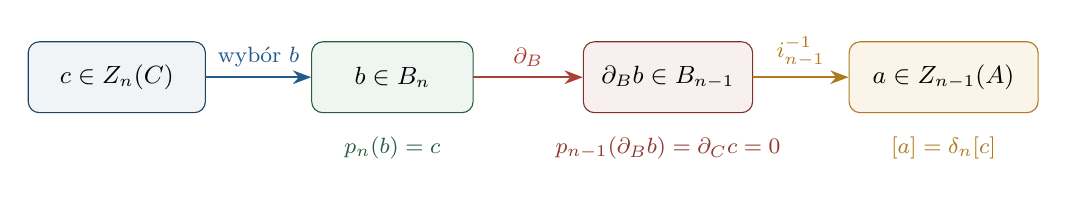
\begin{tikzpicture}[>=Stealth,line cap=round,
  every node/.style={font=\small}]
 \node[draw=manifoldblue!75!black,rounded corners,
  fill=manifoldblue!7,minimum width=2.25cm,
  minimum height=.9cm] (c) at (-5.25,0) {$c\in Z_n(C)$};
 \node[draw=manifoldgreen!75!black,rounded corners,
  fill=manifoldgreen!8,minimum width=2.05cm,
  minimum height=.9cm] (b) at (-1.75,0) {$b\in B_n$};
 \node[draw=manifoldred!75!black,rounded corners,
  fill=manifoldred!8,minimum width=2.15cm,
  minimum height=.9cm] (db) at (1.75,0) {$\partial_Bb\in B_{n-1}$};
 \node[draw=manifoldgold!85!black,rounded corners,
  fill=manifoldgold!10,minimum width=2.4cm,
  minimum height=.9cm] (a) at (5.25,0) {$a\in Z_{n-1}(A)$};
 \draw[->,thick,manifoldblue] (c) --
  node[midway,above,font=\footnotesize] {wybór $b$} (b);
 \draw[->,thick,manifoldred] (b) --
  node[midway,above,font=\footnotesize] {$\partial_B$} (db);
 \draw[->,thick,manifoldgold!85!black] (db) --
  node[midway,above,font=\footnotesize] {$i_{n-1}^{-1}$} (a);
 \node[font=\footnotesize,manifoldgreen!75!black]
  at (-1.75,-.9) {$p_n(b)=c$};
 \node[font=\footnotesize,manifoldred!85!black]
  at (1.75,-.9) {$p_{n-1}(\partial_Bb)=\partial_Cc=0$};
 \node[font=\footnotesize,manifoldgold!85!black]
  at (5.25,-.9) {$[a]=\delta_n[c]$};
\end{tikzpicture}
\caption{Odwzorowanie łączące: podnosimy cykl $c$, bierzemy brzeg
podniesienia $b$, po czym odczytujemy go w $A_{n-1}$.
Odwrócenie $i_{n-1}$ dotyczy tylko jego obrazu
$\ker p_{n-1}$; całego odwzorowania $i_{n-1}$ nie odwracamy.}
\label{fig:homologia-delta}
\end{figure}

\begin{twierdzenie}[Długi ciąg dokładny]
\label{thm:les-homologia}
Z krótkiego ciągu dokładnego kompleksów
otrzymujemy naturalny długi ciąg dokładny
\begin{equation}\label{eq:les-homologia}
 \cdots\longrightarrow H_n(A)
 \xrightarrow{i_*}H_n(B)
 \xrightarrow{p_*}H_n(C)
 \xrightarrow{\delta_n}H_{n-1}(A)
 \xrightarrow{i_*}H_{n-1}(B)
 \longrightarrow\cdots.
\end{equation}
Odwzorowanie \emph{łączące} $\delta_n$ ma następujący
konkretny wzór. Dla cyklu $c\in C_n$ wybieramy
podniesienie $b\in B_n$ z $p_n(b)=c$.
Wtedy $\partial_B b=i_{n-1}(a)$ dla dokładnie
jednego $a\in A_{n-1}$, a
\begin{equation}\label{eq:delta-wzor}
 \delta_n[c]=[a]\in H_{n-1}(A).
\end{equation}
Jeżeli kompleksy są zerowe w ujemnych stopniach,
końcowy fragment ma postać
$H_0(A)\to H_0(B)\to H_0(C)\to0$.
\end{twierdzenie}
\begin{proof}
\emph{Konstrukcja i cykl.} Surjektywność $p_n$
daje podniesienie $b$. Ponieważ $p$ jest odwzorowaniem łańcuchowym,
\[
 p_{n-1}(\partial_Bb)=\partial_C(p_nb)=\partial_Cc=0.
\]
Z dokładności~\eqref{eq:ses-kompleks} w
stopniu $n-1$ mamy
$\partial_Bb\in\ker p_{n-1}=\operatorname{im}i_{n-1}$,
więc istnieje $a$ z $i_{n-1}a=\partial_Bb$.
Iniektywność $i_{n-1}$ daje jego jednoznaczność.
Ponadto
\[
 i_{n-2}(\partial_Aa)
 =\partial_B(i_{n-1}a)=\partial_B^2b=0.
\]
Iniektywność $i_{n-2}$ wymusza $\partial_Aa=0$.
Możemy więc wziąć klasę $[a]$.

\emph{Niezależność od podniesienia.} Jeśli $b'$ też
podnosi $c$, to $b'-b=i_n(u)$ dla pewnego
$u\in A_n$. Wtedy
\[
 \partial_Bb'=\partial_Bb+\partial_Bi_nu
 =i_{n-1}(a+\partial_Au).
\]
Nowy cykl w $A$ różni się od $a$ o brzeg,
więc wyznacza tę samą klasę.

\emph{Niezależność od reprezentanta.}
Niech $c'=c+\partial_Cv$, $v\in C_{n+1}$.
Wybierzmy podniesienie $w\in B_{n+1}$ elementu $v$.
Wtedy $b+\partial_Bw$ podnosi $c'$ i ma ten sam
brzeg co $b$, bo $\partial_B^2w=0$.
Każde inne podniesienie $c'$ różni się od tego
o element $\operatorname{im}i_n$; właśnie
sprawdzona niezależność od podniesienia
kończy dowód niezależności od wyboru reprezentanta klasy $[c]$.
Suma podniesień podnosi sumę cykli, a
podniesienie $rb$ podnosi $rc$, więc $\delta_n$
jest homomorfizmem $R$-modułów.

\emph{Dokładność przy $H_n(B)$.}
Z $pi=0$ mamy $p_*i_*=0$.
Jeśli $[b]\in H_n(B)$ spełnia
$p_*[b]=0$, to dla cyklu $b$
istnieje $v\in C_{n+1}$ z
$p_nb=\partial_Cv$. Wybierzmy podniesienie
$w\in B_{n+1}$ elementu $v$.
Wtedy $b'=b-\partial_Bw$ nadal jest cyklem,
$[b']=[b]$ i
$p_nb'=p_nb-\partial_Cv=0$. Z dokładności
w stopniu $n$ mamy $b'=i_na$.
Ponieważ $\partial_Bb'=i_{n-1}\partial_Aa=0$
i $i_{n-1}$ jest iniektywna, $a$ jest
cyklem. Stąd $[b]=i_*[a]$.

\emph{Dokładność przy $H_n(C)$.}
Jeżeli $c=p_nb$ dla cyklu $b$, możemy
w definicji $\delta_n$ wybrać to właśnie
podniesienie: $\partial_Bb=0$, więc $\delta_n[c]=0$.
Odwrotnie, załóżmy $\delta_n[c]=0$
i podnieśmy cykl $c$ do $b$.
Jeśli $\partial_Bb=i_{n-1}a$, to $[a]=0$,
czyli $a=\partial_Au$ dla pewnego $u\in A_n$.
Element $b-i_nu$ jest cyklem, bo
$\partial_B(b-i_nu)=i_{n-1}(a-\partial_Au)=0$,
a $p_n(b-i_nu)=c$. Zatem
$[c]=p_*[b-i_nu]$.

\emph{Dokładność przy $H_{n-1}(A)$.}
Dla klasy $\delta_n[c]=[a]$ mamy
$i_{n-1}a=\partial_Bb$, czyli $i_*[a]=0$.
Odwrotnie, jeżeli $a\in Z_{n-1}(A)$
i $i_*[a]=0$, istnieje $b\in B_n$
takie, że $i_{n-1}a=\partial_Bb$.
Wówczas $c=p_nb$ jest cyklem, bo
$\partial_Cc=p_{n-1}\partial_Bb=p_{n-1}i_{n-1}a=0$,
a wzór~\eqref{eq:delta-wzor} daje
$\delta_n[c]=[a]$.
Przesuwając indeks $n$ o jeden,
obejmujemy tymi trzema sprawdzeniami
każde miejsce całego ciągu~\eqref{eq:les-homologia}.
W końcu, przy założonej zerowości kompleksów w ujemnych
stopniach mamy $A_{-1}=0$, a więc
$H_{-1}(A)=0$, więc $H_0(B)\to H_0(C)$
jest surjekcją na mocy właśnie wykazanej
dokładności.
\end{proof}

\begin{uwaga}[Naturalność odwzorowania łączącego]
\label{uwaga:les-naturalnosc}
Jeżeli mamy odwzorowanie między dwoma krótkimi
ciągami kompleksów, zgodne z $i,p$ i
różniczkami, to odwzorowania na homologiach
komutują także z $\delta$.
Dokładniej, są to odwzorowania łańcuchowe
$f_A:A\to A'$, $f_B:B\to B'$, $f_C:C\to C'$ spełniające
$f_Bi=i'f_A$ oraz $p'f_B=f_Cp$.
Istotnie, podniesienie $b$ cyklu $c$ przechodzi
w podniesienie obrazu $c$, jego brzeg przechodzi
w obraz $\partial_Bb$, a wstrzyknięcie $i$
pozwala odczytać obraz tego samego $a$.
Równość na reprezentantach ma postać
$\delta'_n(H_n(f_C)[c])
=H_{n-1}(f_A)(\delta_n[c])$.
\end{uwaga}

\begin{przyklad}[Niezerowe odwzorowanie łączące]
\label{prz:delta-izomorfizm}
Niech $A_\bullet$ ma jedyny niezerowy moduł
$A_0=R$, a $C_\bullet$ jedyny niezerowy
moduł $C_1=R$. Niech $B_\bullet$ ma
$B_1=B_0=R$ i różniczkę
$\partial_B=\id_R:B_1\to B_0$.
W stopniu $0$ odwzorowanie $i_0:A_0\to B_0$
jest identycznością, a w stopniu $1$
odwzorowanie $p_1:B_1\to C_1$ jest identycznością;
pozostałe odwzorowania to jedyne możliwe odwzorowania zerowe.
W każdym stopniu otrzymujemy rozszczepiony
krótki ciąg dokładny modułów, ale
$H_n(B)=0$ we wszystkich stopniach.
Cykl $c=1\in C_1$ podnosimy do $b=1\in B_1$.
Jego brzeg to $1=i_0(1)\in B_0$,
więc $\delta_1:R\to R$ jest identycznością.
Przykład pokazuje, że stopniowe rozszczepienie
nie oznacza zgodnego z różniczkami
rozszczepienia kompleksów.
\end{przyklad}
\section{Kohomologia algebraiczna i jej długi ciąg}
\label{sec:kohomologia-algebraiczna}

W homologii różniczka obniża stopień.
Kohomologia powstaje z równie prostej
konstrukcji, w której różniczka stopień
\emph{podwyższa}. Gdy elementy kompleksu
łańcuchowego są wektorami, elementy
kompleksu dualnego są funkcjonałami:
zamiast brać brzeg wektora, oceniamy
funkcjonał na brzegu.

\begin{definicja}[Kompleks kołańcuchowy i kohomologia]
\index{kompleks kolancuchowy i kohomologia@Kompleks kołańcuchowy i kohomologia}
\label{def:kohomologia-algebraiczna}
\emph{Kompleks kołańcuchowy} $K^\bullet$ to
moduły $K^n$ i homomorfizmy
$d^n:K^n\to K^{n+1}$ z
$d^{n+1}d^n=0$ dla $n\in\Z$. Jego \emph{kohomologią stopnia $n$}
jest
\begin{equation}\label{eq:kohomologia-def}
 H^n(K):=\frac{\ker(d^n:K^n\to K^{n+1})}
 {\operatorname{im}(d^{n-1}:K^{n-1}\to K^n)}.
\end{equation}
Elementy jądra nazywamy \emph{kocyklami},
a elementy obrazu \emph{kobrzegami}.
Odwzorowanie kołańcuchowe $F:K^\bullet\to L^\bullet$
składa się z $F^n:K^n\to L^n$ spełniających
$d_L^nF^n=F^{n+1}d_K^n$.
\end{definicja}

Tak jak w dowodzie
Stwierdzenia~\ref{prop:homologia-funktor},
odwzorowanie kołańcuchowe przenosi kocykle w
kocykle i kobrzegi w kobrzegi:
$d_LFz=Fdz=0$ oraz
$F(d_Ku)=d_L(Fu)$. Wobec tego definiuje
$H^n(F)[z]=[F^nz]$. Równość
$H^n(K)=0$ mówi dokładnie, że
$K^{n-1}\to K^n\to K^{n+1}$
jest dokładny w $K^n$.

\begin{przyklad}[Kohomologia dwuwyrazowego kompleksu]
Dla $K^0=K^1=\Z$, $d^0=\times2$
i wszystkich innych modułów równych $0$
otrzymujemy $H^0(K)=0$ oraz
$H^1(K)=\Z/2\Z$. W stopniu $1$ nie ma
już różniczki wychodzącej, więc
wszystkie elementy $\Z$ są kocyklami;
kobrzegami są liczby parzyste.
\end{przyklad}

\begin{stwierdzenie}[Kompleks dualny]
\label{prop:kompleks-dualny}
Dla kompleksu łańcuchowego $C_\bullet$
i $R$-modułu $G$ połóżmy
\[
 C^n(C;G):=\operatorname{Hom}_R(C_n,G),
 \qquad d^n\varphi:=\varphi\circ \partial_{n+1}.
\]
Wtedy $C^\bullet(C;G)$ jest kompleksem
kołańcuchowym. Odwzorowanie łańcuchowe
$f:C_\bullet\to D_\bullet$ daje odwzorowanie
kołańcuchowe w odwrotną stronę,
$f^*:C^\bullet(D;G)\to C^\bullet(C;G)$,
$f^*(\varphi)=\varphi\circ f_n$.
\end{stwierdzenie}
\begin{proof}
Dla $\varphi:C_n\to G$ mamy
\[
 d^{n+1}(d^n\varphi)
 =(\varphi\circ \partial_{n+1})\circ \partial_{n+2}
 =\varphi\circ(\partial_{n+1}\partial_{n+2})=0.
\]
Z kolei dla $\varphi:D_n\to G$
oraz $x\in C_{n+1}$ równość odwzorowań łańcuchowych
z~\eqref{eq:mapa-lancuchowa} daje
\[
 (d f^*\varphi)(x)
 =\varphi(f_n(\partial_C x))
 =\varphi(\partial_D(f_{n+1}x))
 =(f^*d\varphi)(x).
\]
To dowodzi zgodności z różniczką.
\end{proof}

Słowo \emph{dualny} wymaga tu ostrożności:
zastosowanie $\operatorname{Hom}_R(-,G)$
do krótkiego ciągu dokładnego modułów
nie musi dać krótkiego ciągu dokładnego.
Na przykład przy $G=\Z$ w ciągu
$0\to2\Z\hookrightarrow\Z\to\Z/2\Z\to0$
funkcjonał $2\Z\to\Z$, $2k\mapsto k$,
nie przedłuża się do homomorfizmu
$\Z\to\Z$: musiałby wysłać $1$
na liczbę $t$ z $2t=1$.
Z tego powodu nie będziemy budować
długiego ciągu kohomologii przez
bezrefleksyjne dualizowanie
Twierdzenia~\ref{thm:les-homologia}.

\begin{twierdzenie}[Długi ciąg kohomologii]
\label{thm:les-kohomologia}
Jeżeli w każdym stopniu dokładny jest
krótki ciąg \emph{kompleksów kołańcuchowych}
\[
 0\longrightarrow A^\bullet\xrightarrow{i}B^\bullet
 \xrightarrow{p}C^\bullet\longrightarrow0,
\]
to istnieje długi ciąg dokładny
\begin{equation}\label{eq:les-kohomologia}
 \cdots\longrightarrow H^n(A)
 \xrightarrow{i_*}H^n(B)
 \xrightarrow{p_*}H^n(C)
 \xrightarrow{\delta^n}H^{n+1}(A)
 \xrightarrow{i_*}H^{n+1}(B)\longrightarrow\cdots.
\end{equation}
\end{twierdzenie}
\begin{proof}
Dla kocyklu $c\in C^n$ wybierzmy podniesienie
$b\in B^n$ z $p(b)=c$.
Wtedy $p(d_Bb)=d_Cc=0$, więc dokładność
w stopniu $n+1$ i iniektywność $i$
dają dokładnie jedno $a\in A^{n+1}$
z $i(a)=d_Bb$.
Ponieważ $i(d_Aa)=d_B^2b=0$,
otrzymujemy kocykl $a$.
Definiujemy $\delta^n[c]=[a]$.
Jeśli podniesienie $b$ zastąpimy $b+i(u)$,
to $a$ zmienia się na $a+d_Au$.
Jeśli $c$ zastąpimy $c+d_Cv$, to po
wyborze podniesienia $w$ dla $v$ możemy
zastąpić $b$ przez $b+d_Bw$,
co w ogóle nie zmienia $d_Bb$.
Oba wybory prowadzą zatem do tej
samej klasy. Podniesienie sumy można wziąć
jako sumę podniesień, a $rb$ podnosi $rc$ dla $r\in R$.
Zatem $\delta^n$ jest $R$-liniowa.

Sprawdźmy każde z trzech rodzajów miejsc
w~\eqref{eq:les-kohomologia}.
Przy $H^n(B)$ mamy $p_*i_*=0$.
Jeśli $b\in B^n$ jest kocyklem
i $p_*[b]=0$, to $p(b)=d_Cv$
dla pewnego $v\in C^{n-1}$.
Podnieśmy $v$ do $w\in B^{n-1}$.
Wówczas $b-d_Bw$ jest kocyklem
z tą samą klasą co $b$, a jego
obraz przez $p$ wynosi $0$.
Równa się więc $i(a)$ dla pewnego
$a\in A^n$. Z $0=d_Bi(a)=i(d_Aa)$
i iniektywności $i$ dostajemy
$d_Aa=0$, a zatem $[b]=i_*[a]$.

Przy $H^n(C)$ inkluzja
$\operatorname{im}p_*\subseteq\ker\delta^n$
wynika z wybrania jako podniesienia $c=p(b)$
samego kocyklu $b$: jego różniczka jest $0$.
Jeśli odwrotnie $\delta^n[c]=0$,
to dla podniesienia $b$ mamy $d_Bb=i(a)$,
gdzie $a=d_Au$ dla pewnego $u\in A^n$.
Element $b-i(u)$ jest kocyklem,
którego obraz to $c$, więc
$[c]\in\operatorname{im}p_*$.

Przy $H^{n+1}(A)$ element
$i_*\delta^n[c]$ reprezentuje
$i(a)=d_Bb$ i dlatego jest zerowy.
Jeśli z drugiej strony $a\in A^{n+1}$
jest kocyklem i $i_*[a]=0$,
to $i(a)=d_Bb$ dla pewnego
$b\in B^n$. Obraz $c=p(b)$ jest
kocyklem, gdyż $d_Cc=p(d_Bb)=p(i(a))=0$,
a jego odwzorowanie łączące wynosi $[a]$.
Zmiana $n$ daje dokładność także
w pozostałych stopniach. Konstrukcja jest naturalna:
dla zgodnych odwzorowań $f_A,f_B,f_C$ między krótkimi ciągami
podniesieniem $f_C(c)$ jest $f_B(b)$, a jego różniczka to
$f_B(d_Bb)=f_B(i(a))=i'(f_A(a))$.
Stąd $\delta'^n H^n(f_C)=H^{n+1}(f_A)\delta^n$.
\end{proof}

\begin{twierdzenie}[Nad ciałem kohomologia jest dualna do homologii]
\label{thm:field-hom-dual}
Niech $C_\bullet$ będzie kompleksem
przestrzeni liniowych nad ciałem
$\mathbb K$, a
$C^n=\operatorname{Hom}_{\mathbb K}(C_n,\mathbb K)$.
Wtedy naturalne przypisanie
\begin{equation}\label{eq:field-duality}
 H^n(C^\bullet)
 \longrightarrow\operatorname{Hom}_{\mathbb K}
  (H_n(C_\bullet),\mathbb K),
 \qquad [\varphi]\longmapsto
     ([z]\longmapsto\varphi(z))
\end{equation}
jest izomorfizmem. Zakładamy, że
przestrzenie pozwalają na wybór
dopełnień podprzestrzeni
(w szczególności wystarcza skończony wymiar).
\end{twierdzenie}
\begin{proof}
Jeżeli $\varphi\in C^n$ jest kocyklem,
to $d^n\varphi=\varphi \partial_{n+1}=0$.
Zatem $\varphi$ znika na $B_n$,
więc jej wartość na $z\in Z_n$
zależy tylko od klasy $[z]\in H_n$.
Jeżeli zmienimy $\varphi$ na
$\varphi+d^{n-1}\psi
=\varphi+\psi \partial_n$, to dla cyklu $z$
mamy $\partial_nz=0$, więc otrzymujemy
ten sam funkcjonał na $H_n$.
Odwzorowanie~\eqref{eq:field-duality} jest
dobrze określone i liniowe. Jest też naturalne: dla odwzorowania
łańcuchowego $f:C\to D$, kocyklu $\varphi$ na $D$ i cyklu $z$ na $C$
mamy $(f^*\varphi)(z)=\varphi(fz)$. Zatem obie drogi, przez
$H^n(f^*)$ lub przez prekompozycję z $H_n(f)$, dają ten sam funkcjonał.

Aby pokazać surjektywność, weźmy
$\ell:H_n=Z_n/B_n\to\mathbb K$.
Złożenie $Z_n\to H_n\xrightarrow{\ell}\mathbb K$
jest liniowe i znika na $B_n$.
Wybieramy dopełnienie $Z_n$ w $C_n$
i przedłużamy funkcjonał liniowo
na $C_n$, na przykład jako zero
na tym dopełnieniu. Otrzymany
$\varphi$ spełnia
$\varphi \partial_{n+1}=0$, bo
$\operatorname{im}\partial_{n+1}=B_n$;
jest kocyklem wysyłanym na $\ell$.

Jeżeli klasa $[\varphi]$ trafia na zero,
to $\varphi$ znika na całym $Z_n$.
Możemy więc zdefiniować funkcjonał
$\eta$ na $B_{n-1}=\operatorname{im}\partial_n$
przez $\eta(\partial_nx)=\varphi(x)$.
Jest dobrze określony: z
$\partial_nx=\partial_nx'$ wynika $x-x'\in Z_n$,
a tam $\varphi$ znika.
Wybieramy dopełnienie $B_{n-1}$
w $C_{n-1}$ i przedłużamy $\eta$
do $\psi:C_{n-1}\to\mathbb K$.
Wtedy $\varphi=\psi \partial_n=d^{n-1}\psi$
jest kobrzegiem. Jądro odwzorowania
w~\eqref{eq:field-duality} jest więc zerowe.
\end{proof}

\begin{uwaga}[Dlaczego ważne są współczynniki?]
Nad $\Z$ odpowiednik~\eqref{eq:field-duality}
może być fałszywy. Dla kompleksu
$C_1=C_0=\Z$ z $\partial_1=\times2$ mamy
$H_0(C)=\Z/2$ i $H_1(C)=0$,
podczas gdy dla dualnego kompleksu
$H^1(C^\bullet)=\Z/2$.
Grupa $\operatorname{Hom}_{\Z}
(H_1(C),\Z)$ jest zerowa.
Ta dodatkowa klasa kohomologii
wykrywa informację torsyjną z
poprzedniego stopnia. Nie utożsamiamy
więc homologii z kohomologią bez
sprawdzenia założeń o współczynnikach.
\end{uwaga}
\section{Homotopia łańcuchowa i uproszczenia kompleksów}
\label{sec:homotopia-lancuchowa}

Jedna homologia może mieć bardzo różne opisy
przez generatory i różniczki. Poniższe kryterium
mówi, kiedy dwa odwzorowania kompleksów dają
\emph{dokładnie to samo} odwzorowanie na
homologiach. Jest to algebraiczny mechanizm
usuwania par generatorów, które wzajemnie
się kasują.

\begin{definicja}[Homotopia łańcuchowa]
\index{homotopia lancuchowa@Homotopia łańcuchowa}
\label{def:homotopia-lancuchowa}
Dwa odwzorowania łańcuchowe $f,g:C_\bullet\to D_\bullet$
są \emph{łańcuchowo homotopijne}, jeśli istnieją
homomorfizmy $R$-modułów $h_n:C_n\to D_{n+1}$ takie, że
\begin{equation}\label{eq:chain-homotopy}
 f_n-g_n=\partial^D_{n+1}h_n+h_{n-1}\partial^C_n
 \qquad\text{dla każdego }n.
\end{equation}
Kompleks $C_\bullet$ jest \emph{ściągalny},
jeśli $\id_C$ jest łańcuchowo homotopijna
z odwzorowaniem zerowym.
\end{definicja}

Wzór~\eqref{eq:chain-homotopy} przypomina
zasadę całkowania przez części: różnica
odwzorowań składa się z dwóch operacji, w których
$h$ i $\partial$ występują w przeciwnych
kolejnościach. Na cyklach drugi składnik
znika, a pierwszy jest brzegiem.

\begin{twierdzenie}[Homotopia nie zmienia homologii]
\label{thm:homotopia-homologia}
Jeśli $f$ i $g$ są łańcuchowo homotopijne,
to $H_n(f)=H_n(g)$ dla każdego $n$.
W szczególności kompleks ściągalny jest
acykliczny. Jeśli istnieją odwzorowania łańcuchowe
$f:C_\bullet\to D_\bullet$ i
$g:D_\bullet\to C_\bullet$ z
$gf\simeq\id_C$ i $fg\simeq\id_D$,
to $H_n(f)$ i $H_n(g)$ są wzajemnymi
izomorfizmami.
\end{twierdzenie}
\begin{proof}
Dla $z\in Z_n(C)$ równanie~\eqref{eq:chain-homotopy}
redukuje się do
\[
 f_n(z)-g_n(z)=\partial^D_{n+1}h_n(z),
\]
bo $\partial^C_nz=0$. Różnica obrazów jest
brzegiem, więc $[f_n(z)]=[g_n(z)]$.
Gdy $f=\id_C$, $g=0$, otrzymujemy
$[z]=[0]$ dla każdej klasy, czyli
$H_n(C)=0$.
Na koniec, dzięki
Stwierdzeniu~\ref{prop:homologia-funktor},
\[
 H_n(g)H_n(f)=H_n(gf)
 =H_n(\id_C)=\id,\qquad
 H_n(f)H_n(g)=\id.
\]
Stąd oba odwzorowania na homologiach są
odwrotne do siebie.
\end{proof}

\begin{przyklad}[Najprostsze ściągnięcie]
Dla kompleksu
$0\to R\xrightarrow{\id}R\to0$
z modułami w stopniach $1$ i $0$
połóżmy $h_0:R=C_0\to C_1=R$
równe identyczności, a pozostałe
$h_n=0$. W stopniu $0$ mamy
$\partial_1h_0=\id_{C_0}$, a w stopniu
$1$ mamy $h_0\partial_1=\id_{C_1}$.
Wzór~\eqref{eq:chain-homotopy}
daje $\id_C=\partial h+h\partial$.
\end{przyklad}

\begin{twierdzenie}[Algebraiczne skasowanie pary generatorów]
\label{thm:kasowanie-pary}
Niech $C_\bullet$ będzie kompleksem
wolnych $R$-modułów z ustalonymi
bazami, a $n\geq1$. Załóżmy, że
przy generatorze $f\in C_{n-1}$
we współrzędnych $\partial_n(e)$ dla pewnego
generatora $e\in C_n$ stoi skalar
odwracalny $u\in R$.
Wtedy przez zmiany baz można rozłożyć
$C_\bullet$ na sumę prostą
podkompleksu i dwuwyrazowego kompleksu
\[
 0\longrightarrow R e
 \xrightarrow{\ \partial_n\ }R\,\partial_n(e)
 \longrightarrow0,
\]
w którym $\partial_n$ jest izomorfizmem.
Usunięcie tej pary nie zmienia homologii.
\end{twierdzenie}
\begin{proof}
Zapiszmy
$C_n=R e\oplus M$ oraz
$C_{n-1}=R f\oplus N$, gdzie
$M,N$ są rozpięte przez pozostałe
wybrane wektory bazowe.
Z założenia
$\partial_n(e)=u f+v$ z $v\in N$.
Ponieważ $u$ jest odwracalny,
$f':=\partial_n(e)$ może zastąpić $f$
w bazie $C_{n-1}$:
$C_{n-1}=R f'\oplus N$.
Rzeczywiście, $f=u^{-1}(f'-v)$
pozwala przejść w obie strony
między rozkładami.

Dla $x\in M$ zapiszmy
$\partial_n(x)=a(x)f+w(x)$,
gdzie $a(x)\in R$ i $w(x)\in N$.
Zmieńmy też bazę w stopniu $n$,
zastępując każdy bazowy $x\in M$
wektorem $x':=x-u^{-1}a(x)e$.
Wtedy
\[
 \partial_n(x')
 =a(x)f+w(x)-u^{-1}a(x)(uf+v)
 =w(x)-u^{-1}a(x)v\in N.
\]
Nowe wektory $x'$ razem z $e$
tworzą bazę $C_n$: możemy odzyskać
$x=x'+u^{-1}a(x)e$.
Oznaczmy ich rozpiętość przez $M'$.
Mamy zatem $\partial_n(Re)=Rf'$
i $\partial_n(M')\subseteq N$.

Równość $\partial_{n-1}(f')=\partial_{n-1}\partial_n(e)=0$
mówi, że z $Rf'$ nie wychodzi
różniczka. Z kolei dla $y\in C_{n+1}$
zapiszmy $\partial_{n+1}(y)=t e+x'$,
$x'\in M'$. Po zastosowaniu $\partial_n$
dostajemy
$0=\partial_n\partial_{n+1}(y)=t f'+\partial_n(x')$.
Pierwszy składnik należy do $Rf'$,
drugi do $N$; rozkład jest prosty,
więc $t=0$. Żadna różniczka
z wyższego stopnia nie trafia do $Re$.
Pozostałe moduły wraz z $M'$ i $N$
tworzą więc podkompleks, a
$Re\xrightarrow{\cong}Rf'$
jest jego prostym składnikiem
w całym kompleksie.

Na tym dwuwyrazowym składniku
homotopia $h_{n-1}(f')=e$,
zerowa w innych stopniach,
spełnia $\id=\partial h+h\partial$.
Jest on ściągalny. Przedłużmy tę homotopię przez zero na
pozostałym podkompleksie $D$. Dla rzutu $p:C\to D$ i włączenia
$j:D\to C$ otrzymujemy $pj=\id_D$ oraz
$\id_C-jp=\partial h+h\partial$. Rzut i włączenie
wyznaczają odwrotne izomorfizmy
na homologiach na mocy
Twierdzenia~\ref{thm:homotopia-homologia}.
\end{proof}

Nad $\Z$ jednostkami są tylko $1$ i $-1$.
Współczynnik $2$ w różniczce
$\Z\xrightarrow{\times2}\Z$ nie pozwala
wykonać takiego skasowania: pozostała
klasa $\Z/2$ z
Przykładu~\ref{prz:homologia-rachunki}
jest rzeczywistą przeszkodą.

\begin{stwierdzenie}[Acykliczny kompleks przestrzeni liniowych]
\label{prop:acykliczny-sciagalny}
Jeżeli $C_\bullet$ jest kompleksem
przestrzeni liniowych nad ciałem
$\mathbb K$ i $H_n(C)=0$ dla wszystkich
$n$, to $C_\bullet$ jest ściągalny.
Wystarczy, aby każda podprzestrzeń
$Z_n(C)\subseteq C_n$ miała dopełnienie;
warunek ten zachodzi zawsze przy
skończonych wymiarach.
\end{stwierdzenie}
\begin{proof}
Acykliczność daje $Z_n=B_n$.
Wybierzmy dopełnienie $S_n$ tak, aby
$C_n=Z_n\oplus S_n$. Ograniczenie
\[
 \partial_n|_{S_n}:S_n\longrightarrow Z_{n-1}
\]
jest iniektywne: element jego jądra
należy do $S_n\cap Z_n=\{0\}$.
Jest też surjektywne, bo
$\partial_n(C_n)=B_{n-1}=Z_{n-1}$
i $\partial_n$ znika na $Z_n$.
Ma więc odwrotność.
Każde $x\in C_n$ zapiszmy
jednoznacznie jako $x=z+s$
z $z\in Z_n$, $s\in S_n$, i połóżmy
\[
 h_n(z+s)
 :=(\partial_{n+1}|_{S_{n+1}})^{-1}(z)
 \in S_{n+1}.
\]
Wówczas $\partial_{n+1}h_n(z+s)=z$.
Z drugiej strony $\partial_n(z+s)=\partial_n(s)$,
więc
$h_{n-1}\partial_n(z+s)
=(\partial_n|_{S_n})^{-1}(\partial_ns)=s$.
Zatem $(\partial h+h\partial)(x)=z+s=x$
w każdym stopniu.
\end{proof}

\begin{przyklad}[Acykliczny, lecz nieściągalny nad $\Z$]
\label{prz:acykliczny-niesciagalny}
Potraktujmy dokładny ciąg z
Przykładu~\ref{prz:ses-mod-m} dla $m=2$
jako kompleks w stopniach $2,1,0$:
\[
 0\longrightarrow\Z\xrightarrow{\ \times2\ }\Z
 \xrightarrow{\ \pi\ }\Z/2\Z\longrightarrow0.
\]
Jego wszystkie homologie są zerowe,
bo $\times2$ jest iniekcją,
$\ker\pi=2\Z$, a $\pi$ jest
surjekcją. Gdyby kompleks był
ściągalny, to w stopniu $0$
wzór $\id=\partial h+h\partial$ dałby
$\id_{\Z/2}=\pi h_0$.
Odwzorowanie $h_0:\Z/2\to\Z$ byłoby
przekrojem $\pi$, którego
nie ma według uwagi po
Twierdzeniu~\ref{thm:ses-rozszczepienie}.
Zatem implikacja \emph{acykliczny
$\Rightarrow$ ściągalny} wymaga
dodatkowych założeń. Implikacja
odwrotna z
Twierdzenia~\ref{thm:homotopia-homologia}
działa nad każdym pierścieniem.
\end{przyklad}

\section{Ilorazy, ciągi względne i filtracje}
\label{sec:iloraz-filtracja}

Podkompleks $A_\bullet\subseteq C_\bullet$
oznacza podmoduły $A_n\subseteq C_n$
we wszystkich stopniach, takie że
$\partial_C(A_n)\subseteq A_{n-1}$.
Definiujemy \emph{kompleks ilorazowy}
$(C/A)_n=C_n/A_n$ i
$\partial_{C/A}[c]=[\partial_Cc]$.
Jeśli $[c]=[c+a]$ dla $a\in A_n$,
to $[\partial_Cc]=[\partial_Cc+\partial_Ca]$;
różniczka ilorazowa jest dobrze
określona i jej kwadrat wynosi zero.

\begin{stwierdzenie}[Długi ciąg ilorazu]
\label{prop:ses-iloraz}
Dla podkompleksu $A_\bullet\subseteq C_\bullet$
ciąg
\[
 0\longrightarrow A_\bullet
 \longrightarrow C_\bullet
 \longrightarrow C_\bullet/A_\bullet
 \longrightarrow0
\]
jest stopniowo dokładny. Dlatego istnieje
długi ciąg
\begin{equation}\label{eq:les-iloraz}
 \cdots\to H_n(A)\to H_n(C)\to H_n(C/A)
 \xrightarrow{\delta_n}H_{n-1}(A)\to\cdots.
\end{equation}
Jeśli $\xi\in H_n(C/A)$, to możemy
reprezentować ją elementem $c\in C_n$
z $\partial_Cc\in A_{n-1}$, a wtedy
$\delta_n\xi=[\partial_Cc]$. Tutaj $c$ najpierw wyznacza cykl
$c+A_n$ w kompleksie ilorazowym, a dopiero jego klasa modulo
brzegi jest elementem $\xi$; są to dwa różne przejścia do ilorazu.
\end{stwierdzenie}
\begin{proof}
W każdym stopniu włączenie $A_n\to C_n$
jest iniekcją, projekcja $C_n\to C_n/A_n$
jest surjekcją, a jej jądrem jest $A_n$.
Oba odwzorowania komutują z różniczkami
z definicji podkompleksu i ilorazu.
Twierdzenie~\ref{thm:les-homologia}
stosuje się więc bez dodatkowych
założeń. Warunek
$\partial_{C/A}[c]=[0]$ jest równoważny
$\partial_Cc\in A_{n-1}$; w tej sytuacji
konstrukcja~\eqref{eq:delta-wzor}
przy podniesieniu $c$ daje dokładnie
klasę $[\partial_Cc]$.
\end{proof}

Symbol $H_n(C,A):=H_n(C/A)$ będziemy
nazywać \emph{względną homologią
algebraiczną} kompleksu $C$ względem
podkompleksu $A$. Jest to definicja
czysto algebraiczna. W przyszłych
konstrukcjach topologicznych trzeba
osobno sprawdzić, że odpowiednie
łańcuchy tworzą podkompleks.

\begin{stwierdzenie}[Względna kohomologia nad ciałem]
\label{prop:wzgledna-kohomologia}
Jeśli $A_\bullet\subseteq C_\bullet$
jest podkompleksem przestrzeni liniowych
nad ciałem $\mathbb K$, to wzięcie
funkcjonałów daje krótki ciąg dokładny
kompleksów kołańcuchowych
\[
 0\to\operatorname{Hom}_{\mathbb K}
      (C/A,\mathbb K)
 \to\operatorname{Hom}_{\mathbb K}(C,\mathbb K)
 \to\operatorname{Hom}_{\mathbb K}(A,\mathbb K)
 \to0.
\]
Jeśli $H^n(C,A;\mathbb K)$ oznacza
kohomologię pierwszego z nich, to mamy
długi ciąg
\[
 \cdots\to H^n(C,A;\mathbb K)\to H^n(C;\mathbb K)
 \to H^n(A;\mathbb K)\to H^{n+1}(C,A;\mathbb K)
 \to\cdots .
\]
W tym zapisie $H^n(C;\mathbb K)$
oznacza kohomologię kompleksu
$\operatorname{Hom}_{\mathbb K}(C,\mathbb K)$,
a analogicznie dla $A$.
\end{stwierdzenie}
\begin{proof}
W stopniu $n$ pierwsze odwzorowanie składa
funkcjonał $C_n/A_n\to\mathbb K$
z projekcją $C_n\to C_n/A_n$,
więc jest iniektywne.
Drugie ogranicza funkcjonał na $C_n$
do podprzestrzeni $A_n$.
Jego jądrem są dokładnie funkcjonały
znikające na $A_n$, czyli faktoryzujące
się przez $C_n/A_n$; to obraz
pierwszego odwzorowania. Każdy funkcjonał
na $A_n$ przedłuża się do $C_n$:
wybieramy dopełnienie $A_n$
i stawiamy na nim wartość $0$.
Drugie odwzorowanie jest zatem surjektywne.
Odwzorowania komutują z różniczkami
kołańcuchowymi, bo są zdefiniowane
przez składanie z odwzorowaniami łańcuchowymi.
Stosujemy
Twierdzenie~\ref{thm:les-kohomologia}.
\end{proof}

\begin{stwierdzenie}[Trzy zagnieżdżone kompleksy]
\label{prop:les-potrojny}
Jeśli $A_\bullet\subseteq B_\bullet
\subseteq C_\bullet$, to istnieje
krótki ciąg dokładny kompleksów
\[
 0\longrightarrow B_\bullet/A_\bullet
 \longrightarrow C_\bullet/A_\bullet
 \longrightarrow C_\bullet/B_\bullet
 \longrightarrow0
\]
i wynikający z niego długi ciąg
\[
 \cdots\to H_n(B,A)\to H_n(C,A)\to H_n(C,B)
 \to H_{n-1}(B,A)\to\cdots.
\]
\end{stwierdzenie}
\begin{proof}
W stopniu $n$ pierwsze odwzorowanie
$[b]_A\mapsto[b]_A$ jest iniektywne:
jeśli $[b]_A=0$ w $C_n/A_n$, to
$b\in A_n$, więc była już zerowa w
$B_n/A_n$. Ostatnie odwzorowanie
$[c]_A\mapsto[c]_B$ jest dobrze
określone, bo $A_n\subseteq B_n$,
i surjektywne, bo każda klasa modulo
$B_n$ ma reprezentanta $c\in C_n$.
Jej jądro składa się z klas
$[c]_A$ z $c\in B_n$, czyli jest
obrazem pierwszego odwzorowania.
Różniczki zachowują wszystkie trzy
podkompleksy, więc są to odwzorowania
kompleksów. Stosujemy
Twierdzenie~\ref{thm:les-homologia}.
\end{proof}

\begin{definicja}[Filtracja kompleksu]
\index{filtracja kompleksu@Filtracja kompleksu}
\label{def:filtracja-kompleksu}
Przez \emph{skończoną filtrację rosnącą} rozumiemy tutaj ciąg
podkompleksów
\[
 0=F_{-1}C_\bullet\subseteq
 F_0C_\bullet\subseteq\cdots\subseteq
 F_NC_\bullet=C_\bullet.
\]
Iloraz $F_pC/F_{p-1}C$ opisuje
algebraicznie \emph{nową warstwę}
w kroku $p$. W każdym kroku mamy
krótki ciąg dokładny
$0\to F_{p-1}C\to F_pC\to
F_pC/F_{p-1}C\to0$
i odpowiadający mu długi ciąg homologii.
\end{definicja}

\begin{wniosek}[Zmiana skoncentrowana w jednym stopniu]
\label{wn:filtracja-jeden-stopien}
Niech $A\subseteq B$ będzie podkompleksem
w nieujemnych stopniach i niech
$H_j(B/A)=0$ dla $j\ne q$, $q\geq1$.
Wówczas $H_j(A)\to H_j(B)$ jest
izomorfizmem dla $j\notin\{q,q-1\}$,
a pozostałe zmiany opisuje ciąg
\begin{equation}\label{eq:jedna-warstwa}
 0\to H_q(A)\to H_q(B)\to H_q(B/A)
 \xrightarrow{\delta_q}H_{q-1}(A)
 \to H_{q-1}(B)\to0.
\end{equation}
\end{wniosek}
\begin{proof}
Dla dowolnego $j$ wytnijmy z~\eqref{eq:les-iloraz}
fragment
\[
 H_{j+1}(B/A)\to H_j(A)\to H_j(B)\to H_j(B/A).
\]
Jeśli oba zewnętrzne moduły są zerowe,
środkowe odwzorowanie jest jednocześnie
iniektywne i surjektywne.
Tak jest, gdy $j\ne q,q-1$.
Dla $j=q$ i $j=q-1$ zachowujemy
pełen fragment długiego ciągu.
Jego lewa skrajna strzałka wychodzi
z $H_{q+1}(B/A)=0$, a prawa
wchodzi do $H_{q-1}(B/A)=0$,
co daje dokładnie~\eqref{eq:jedna-warstwa}.
\end{proof}

\begin{uwaga}[Co mówi odwzorowanie łączące?]
W~\eqref{eq:jedna-warstwa} element
nowej warstwy może zwiększyć
$H_q(B)$, jeśli ma zerowy obraz
przez $\delta_q$. Może też sprawić,
że wcześniejsza klasa w
$H_{q-1}(A)$ stanie się brzegiem:
tak dzieje się, jeśli leży w
$\operatorname{im}\delta_q$.
Ten jeden fragment ciągu odróżnia
\emph{powstanie klasy} od
\emph{zabicia klasy}, bez odwoływania
się do szczególnej realizacji
geometrycznej kompleksu.
\end{uwaga}
\section{Suma podkompleksów i ciąg Mayera--Vietorisa}
\label{sec:mv-algebraiczny}

Przy rozbiciu obiektu na dwie części trzeba
uwzględnić elementy wspólne: bez tego
zliczylibyśmy je dwa razy. Poniższy wynik
jest czysto algebraicznym źródłem
późniejszych ciągów Mayera--Vietorisa.
Nie wymaga jeszcze żadnej konstrukcji
łańcuchów z przestrzeni topologicznej.

\begin{twierdzenie}[Algebraiczny Mayer--Vietoris]
\label{thm:mv-algebraiczny}
Niech $A_\bullet$ i $B_\bullet$ będą
podkompleksami $C_\bullet$. Wtedy
$A\cap B$ i $A+B$ też są podkompleksami,
a ciąg
\begin{equation}\label{eq:mv-ses}
 0\longrightarrow A\cap B
 \xrightarrow{\ j\ }A\oplus B
 \xrightarrow{\ q\ }A+B
 \longrightarrow0,
 \quad j(x)=(x,-x),\quad q(a,b)=a+b
\end{equation}
jest krótkim ciągiem dokładnym kompleksów.
W szczególności mamy długi ciąg dokładny
\begin{equation}\label{eq:mv-les}
 \cdots\to H_n(A\cap B)\to H_n(A)\oplus H_n(B)
 \to H_n(A+B)\xrightarrow{\delta}
 H_{n-1}(A\cap B)\to\cdots.
\end{equation}
Jeśli cykl $c\in(A+B)_n$ zapiszemy
$c=a+b$ z $a\in A_n$, $b\in B_n$,
to $\delta[c]=[\partial a]=[-\partial b]$.
\end{twierdzenie}
\begin{proof}
Jeśli $x\in A_n\cap B_n$, to
$\partial x\in A_{n-1}$ i $\partial x\in B_{n-1}$,
więc $\partial$ zachowuje przecięcie.
Podobnie $\partial(a+b)=\partial a+\partial b$ należy do
$A_{n-1}+B_{n-1}$, zatem suma
też jest podkompleksem.
Różniczka w $A\oplus B$ działa
składowo, dlatego
$\partial\,j(x)=(\partial x,-\partial x)=j(\partial x)$ i
$\partial\,q(a,b)=\partial(a+b)=q(\partial a,\partial b)$.
Są to odwzorowania łańcuchowe.

W każdym stopniu odwzorowanie $j$ jest
iniektywne, bo $j(x)=(0,0)$
implikuje $x=0$. Odwzorowanie $q$ jest
surjektywne na $A_n+B_n$ z samej
definicji sumy. Jeśli $q(a,b)=0$,
to $a=-b$ należy jednocześnie do
$A_n$ i do $B_n$, a para ma postać
$(a,-a)=j(a)$. Stąd
$\ker q=\operatorname{im}j$.
Twierdzenie~\ref{thm:les-homologia}
daje~\eqref{eq:mv-les}. Używamy przy tym kanonicznego izomorfizmu
$H_n(A\oplus B)\cong H_n(A)\oplus H_n(B)$:
różniczka działa składowo, więc cykle i brzegi są odpowiednio
$Z_n(A)\oplus Z_n(B)$ i $B_n(A)\oplus B_n(B)$,
a $[(a,b)]\mapsto([a],[b])$ jest izomorfizmem ich ilorazów.

Na koniec, jeśli $\partial(a+b)=0$, to
$\partial a=-\partial b$. Lewa strona należy do
$A_{n-1}$, prawa do $B_{n-1}$,
więc obie są elementem $A\cap B$.
W konstrukcji odwzorowania łączącego
podniesienie cyklu $c$ jest parą $(a,b)$,
a jej brzeg $(\partial a,\partial b)=(\partial a,-\partial a)$
jest obrazem $j(\partial a)$. To daje
podany wzór i objaśnia znak.
\end{proof}

\begin{przyklad}[Niezerowy brzeg z przecięcia]
\label{prz:mv-niezerowa-delta}
Nad ciałem $\mathbb K$ weźmy kompleks
z $C_1=\mathbb K u\oplus\mathbb K v$,
$C_0=\mathbb K x\oplus\mathbb K y$,
$\partial(u)=x-y$ i $\partial(v)=y-x$,
zerowy w pozostałych stopniach.
Niech $A_1=\mathbb K u$, $B_1=\mathbb K v$,
ale $A_0=B_0=C_0$. Są to podkompleksy,
$A+B=C$, zaś $A\cap B$ jest
skoncentrowany w stopniu $0$
i ma tam moduł $\mathbb K x\oplus\mathbb K y$.
Element $u+v$ jest cyklem w $C_1$.
Jego podniesienie do $A_1\oplus B_1$ to $(u,v)$,
którego brzeg wynosi
$(x-y,y-x)=j(x-y)$. Stąd
\[
 \delta[u+v]=[x-y]
 \in H_0(A\cap B)=\mathbb K x\oplus\mathbb K y,
\]
klasa niezerowa. Widzimy, jak brzeg
jednej części zostaje zniesiony
przez brzeg drugiej i powstaje
cykl w ich sumie.
\end{przyklad}

\section{Współczynniki, torsja i charakterystyka Eulera}
\label{sec:wspolczynniki-euler}

Wybór pierścienia $R$ wpływa na
wynik homologiczny. Kompleks
wolnych grup abelowych
można sprowadzić modulo $m$,
lecz homologia po tej operacji
nie polega zawsze wyłącznie
na redukcji dawnej homologii:
dochodzi torsja z poprzedniego stopnia.

\begin{twierdzenie}[Redukcja współczynników modulo $m$]
\label{thm:mod-m-homologia}
Niech $C_\bullet$ będzie kompleksem
wolnych grup abelowych, a $m\geq2$.
Różniczki wyznaczają kompleks
$(C/mC)_n=C_n/mC_n$. Dla każdego
$n$ istnieje krótki ciąg dokładny
\begin{equation}\label{eq:mod-m-homologia}
 0\longrightarrow H_n(C)/mH_n(C)
 \longrightarrow H_n(C/mC)
 \longrightarrow H_{n-1}(C)[m]
 \longrightarrow0,
\end{equation}
gdzie $H_{n-1}(C)[m]:=
\{x\in H_{n-1}(C):mx=0\}$
to $m$-torsja z Definicji~\ref{def:torsja}.
Nie twierdzimy, że ten ciąg ma
kanoniczne rozszczepienie.
\end{twierdzenie}
\begin{proof}
Wolna grupa abelowa nie ma
niezerowych elementów zabijanych
przez $m$. W każdym stopniu mamy
zatem dokładny ciąg
\[
 0\to C_n\xrightarrow{\ \times m\ }C_n
 \xrightarrow{\ \pi\ }C_n/mC_n\to0.
\]
Ponieważ $\partial(mx)=m\,\partial(x)$,
odwzorowania $\times m$ i $\pi$
komutują z różniczkami.
To krótki ciąg dokładny
kompleksów, więc
Twierdzenie~\ref{thm:les-homologia}
daje fragment
\[
 H_n(C)\xrightarrow{\ \times m\ }H_n(C)
 \xrightarrow{\ \pi_*\ }H_n(C/mC)
 \xrightarrow{\ \delta\ }H_{n-1}(C)
 \xrightarrow{\ \times m\ }H_{n-1}(C).
\]
Dokładność mówi
$\ker\pi_*=mH_n(C)$, a więc
$\pi_*$ wyznacza iniekcję
$H_n(C)/mH_n(C)\hookrightarrow H_n(C/mC)$
o obrazie $\ker\delta$.
Mówi też
$\operatorname{im}\delta
=\ker(\times m:H_{n-1}(C)\to H_{n-1}(C))
=H_{n-1}(C)[m]$.
Odwzorowanie $\delta$ po ograniczeniu
przeciwdziedziny do tego jądra
jest więc surjektywne.
To dokładnie trzy warunki
ciągu~\eqref{eq:mod-m-homologia}.
Warto zapisać ostatnią strzałkę jawnie. Jeśli $\bar c$ jest cyklem
modulo $m$ i $c\in C_n$ jest jego przedstawicielem, to
$\partial c=ma$ dla pewnego $a\in C_{n-1}$.
Element $a$ jest jednoznaczny, bo mnożenie przez $m$ jest iniektywne.
Ponadto $m\partial a=0$ wymusza $\partial a=0$,
a $m[a]=[\partial c]=0$. Zatem strzałka wysyła $[\bar c]$ na $[a]$.
Jest naturalna względem odwzorowań łańcuchowych, gdyż
$\partial f(c)=mf(a)$; pierwsza strzałka wysyła klasę cyklu
$[z]$ modulo $mH_n(C)$ na klasę $z$ modulo $m$.
\end{proof}

\begin{przyklad}[Nowa homologia po redukcji]
Dla $C_1=C_0=\Z$ i $\partial_1=\times2$
otrzymaliśmy $H_1(C)=0$ oraz
$H_0(C)=\Z/2$. Po redukcji modulo
$2$ różniczka $\times2$ staje się
zerowa, a więc
$H_1(C/2C)\cong H_0(C/2C)\cong\Z/2$.
Nowa klasa stopnia $1$ pochodzi
w~\eqref{eq:mod-m-homologia} z
$H_0(C)[2]=\Z/2$, choć wcześniejsze
$H_1(C)$ było zerowe.
\end{przyklad}

\begin{uwaga}[Iloczyn tensorowy modułów i rozszerzenie skalarów]
\label{uwaga:tensor-modulow}
Konstrukcję $M\otimes_R N$, rozszerzenie skalarów
i wpływ tensorowania na surjekcje i iniekcje
udowodniliśmy w Sekcji~\ref{sec:tensor-modulow-algebra}.
Tutaj stosujemy ją do grup łańcuchów; w szczególności
możemy pisać $C_n\otimes_{\Z}\mathbb F$ dla ciała
$\mathbb F$ zawierającego $\Q$.
\end{uwaga}

\begin{definicja}[Homologia ze współczynnikami w $\Q$, $\R$ lub $\C$]
\label{def:homologia-ciala-char-zero}
Niech $(C_\bullet,\partial)$ będzie kompleksem
wolnych grup abelowych, na przykład
kompleksem łańcuchów symplicjalnych.
Dla $\mathbb F\in\{\Q,\R,\C\}$ tworzymy
\[
 C_n(C;\mathbb F):=C_n\otimes_{\Z}\mathbb F,
 \qquad
 \partial_{\mathbb F}(c\otimes a)
       :=(\partial c)\otimes a.
\]
Jeśli $C_n$ ma bazę sympleksów, nowy kompleks
ma tę samą bazę, lecz można przy nich stawiać
współczynniki z $\mathbb F$ zamiast liczb całkowitych.
Jego homologię oznaczamy $H_n(C;\mathbb F)$;
dla kompleksu przypisanego przestrzeni $X$
piszemy $H_n(X;\mathbb F)$.
Piszemy też $H_n(C;\Z)=H_n(C)$ dla pierwotnego kompleksu.
Różniczka jest dobrze określona przez własność uniwersalną,
a $\partial_{\mathbb F}^2=0$ sprawdzamy na tensorach prostych.
\end{definicja}

\begin{twierdzenie}[Co zmienia przejście do charakterystyki zero]
\label{thm:homologia-char-zero}
Dla każdego kompleksu wolnych grup abelowych
i $\mathbb F=\Q,\R$ lub $\C$ istnieje naturalny
izomorfizm
\begin{equation}\label{eq:homologia-char-zero}
 H_n(C;\mathbb F)
 \cong H_n(C;\Z)\otimes_{\Z}\mathbb F.
\end{equation}
Jeśli $H_n(C;\Z)\cong\Z^{b_n}\oplus T_n$,
gdzie $T_n$ jest skończoną grupą torsyjną, to
$H_n(C;\mathbb F)\cong\mathbb F^{b_n}$.
W szczególności w tych trzech ciałach
pozostaje ta sama liczba $b_n$ niezależnych
klas, a torsja znika.
\end{twierdzenie}
\begin{proof}
Najpierw rozważmy $\mathbb F=\Q$.
Element $C_n\otimes_{\Z}\Q$ jest skończoną
sumą prostych tensorów; sprowadzając
mianowniki do wspólnego, zapisujemy go jako
$c/d$ z $c\in C_n$ i niezerowym
$d\in\Z$. Ponieważ każda grupa $C_j$
jest wolna, odwzorowania
$C_j\to C_j\otimes_{\Z}\Q$ są iniektywne.
Jeśli $c/d$ jest cyklem, to
$\partial c/d=0$, a więc $\partial c=0$.
Każda klasa racjonalna pochodzi zatem
całkowitego cyklu po dopuszczeniu mianownika:
odwzorowanie
\[
 H_n(C;\Z)\otimes_{\Z}\Q\longrightarrow H_n(C;\Q),
 \qquad [c]\otimes q\longmapsto[c\otimes q]
\]
jest surjektywne. Jest ono dobrze określone,
bo cykl pozostaje cyklem, brzeg pozostaje
brzegiem, a reguła jest dwuliniowa nad $\Z$.
Każdy tensor w dziedzinie ma postać $[c]\otimes(1/d)$
po sprowadzeniu skończenie wielu ułamków do wspólnego mianownika.

Sprawdźmy, czy nie utożsamia zbyt wielu klas.
Załóżmy, że cykl $c/d$ jest brzegiem
w kompleksie racjonalnym. Istnieją
$b\in C_{n+1}$ i $e\ne0$ takie, że
$c/d=\partial b/e$. Po pomnożeniu przez
$de$ i użyciu iniektywności
$C_n\to C_n\otimes\Q$ otrzymujemy
$ec=d\,\partial b=\partial(db)$
już w $C_n$. To znaczy, że $e[c]=0$
w $H_n(C;\Z)$. Po przejściu do $\Q$
liczba $e$ jest odwracalna, więc
$[c]\otimes(1/d)=0$. Odwzorowanie jest
również iniektywne i wzór został
udowodniony dla $\Q$.

Teraz $\mathbb F=\R$ albo $\C$.
Są to przestrzenie liniowe nad $\Q$, a
rozszerzenie skalarów daje izomorfizm
kompleksów
\[
 C_\bullet\otimes_{\Z}\mathbb F
 \cong (C_\bullet\otimes_{\Z}\Q)
             \otimes_{\Q}\mathbb F.
\]
Jawnie, $(c\otimes q)\otimes a\mapsto c\otimes qa$,
a odwrotnie $c\otimes a\mapsto(c\otimes1)\otimes a$.
Relacje tensorowe pokazują, że oba wzory są dobrze określone
i wzajemnie odwrotne; komutują też z różniczkami.
Wyjaśnijmy, dlaczego tensorowanie kompleksu
przestrzeni liniowych nad ciałem zachowuje
homologię. Oznaczmy na chwilę
$D_\bullet=C_\bullet\otimes_{\Z}\Q$,
$Z_n^\Q=\ker(\partial:D_n\to D_{n-1})$
oraz $B_n^\Q=\operatorname{im}(\partial:D_{n+1}\to D_n)$.
W każdym stopniu uzupełniamy bazy, aby zapisać
$Z_n^\Q=B_n^\Q\oplus V_n$ i
$D_n=Z_n^\Q\oplus L_n$.
Wtedy $\partial:L_n\to B_{n-1}^\Q$ jest
izomorfizmem: surjektywność wynika z definicji
$B_{n-1}^\Q$, a jądro to
$L_n\cap Z_n^\Q=0$. Ponadto
$V_n\cong Z_n^\Q/B_n^\Q=H_n(D)$.
Po tensorowaniu nad $\Q$ rozkłady nadal
są sumami prostymi, a ograniczenie
$\partial\otimes1:L_n\otimes\mathbb F
\to B_{n-1}^\Q\otimes\mathbb F$ pozostaje
izomorfizmem. Nowa homologia to więc
$V_n\otimes\mathbb F
\cong H_n(D)\otimes_{\Q}\mathbb F$.
Łącząc to z przypadkiem $\Q$, otrzymujemy
\eqref{eq:homologia-char-zero} dla $\R,\C$.
Choć dopełnienia ułatwiły dowód bijektywności, sam izomorfizm
jest kanoniczny: we wszystkich trzech przypadkach jest zadany
przez $[z]\otimes a\mapsto[z\otimes a]$.
Równość $f(z)\otimes a=(f\otimes\id)(z\otimes a)$ dowodzi
naturalności względem odwzorowań łańcuchowych.

Wreszcie $\Z\otimes_{\Z}\mathbb F\cong\mathbb F$.
Jeśli $mx=0$ w $T_n$, to
$m(x\otimes a)=0$; ponieważ $m\ne0$
ma odwrotność w $\mathbb F$,
$x\otimes a=0$. Zatem $T_n\otimes\mathbb F=0$,
a $b_n$ generatorów części wolnej daje
$\mathbb F^{b_n}$.
\end{proof}

Warto porównać to z Twierdzeniem~\ref{thm:mod-m-homologia}.
W ciele $\Q$, $\R$ lub $\C$ każda niezerowa
liczba całkowita staje się odwracalna.
Przy współczynnikach modulo $p$ liczba $p$
staje się natomiast \emph{zerem}; torsja
może wtedy dać nowe klasy także w innym stopniu.
Przejście do $\R$ lub $\C$ po obliczeniu
homologii nad $\Q$ jest już tylko
rozszerzeniem skalarów:
\[
 H_n(C;\R)\cong H_n(C;\Q)\otimes_{\Q}\R,
 \qquad
 H_n(C;\C)\cong H_n(C;\R)\otimes_{\R}\C.
\]

\begin{twierdzenie}[Algebraiczna charakterystyka Eulera]
\label{thm:euler-homologia}
Niech $C_\bullet$ będzie kompleksem
skończenie wymiarowych przestrzeni
liniowych nad ciałem $\mathbb K$
i niech tylko skończenie wiele $C_n$
będzie niezerowych. Wtedy
\begin{equation}\label{eq:euler-homologia}
 \sum_n(-1)^n\dim_{\mathbb K}C_n
 =\sum_n(-1)^n\dim_{\mathbb K}H_n(C).
\end{equation}
Lewą stronę nazywamy \emph{charakterystyką
Eulera kompleksu}.
\end{twierdzenie}
\begin{proof}
Odwzorowanie $\partial_n:C_n\to B_{n-1}$ jest
surjektywne z definicji obrazu,
a jego jądro to $Z_n$.
Wybór bazy $Z_n$ i jej uzupełnienie
do bazy $C_n$ pokazują
\[
 \dim C_n=\dim Z_n+\dim B_{n-1}.
\]
Podobnie projekcja $Z_n\to H_n=Z_n/B_n$
ma jądro $B_n$, więc
$\dim Z_n=\dim B_n+\dim H_n$.
Łącząc te równości, otrzymujemy
\[
 \dim C_n=\dim B_n+\dim H_n+\dim B_{n-1}.
\]
Mnożymy przez $(-1)^n$ i sumujemy
po $n$. Suma
$\sum_n(-1)^n\dim B_n$
znosi się z
$\sum_n(-1)^n\dim B_{n-1}$:
po podstawieniu $j=n-1$
druga jest równa
$-\sum_j(-1)^j\dim B_j$.
Skończona liczba niezerowych
wyrazów pozwala to wykonać bez
kłopotów ze zbieżnością.
Pozostaje~\eqref{eq:euler-homologia}.
\end{proof}

\begin{przyklad}[Wykrywanie brakującego wymiaru]
Niech nad $\mathbb K$ mamy tylko
$C_2\cong\mathbb K^2$, $C_1\cong\mathbb K^5$
i $C_0\cong\mathbb K^4$.
Niezależnie od szczegółów różniczek
spełniających $\partial^2=0$, musi zachodzić
\[
 \dim H_0-\dim H_1+\dim H_2
 =4-5+2=1.
\]
Nie można zatem uzyskać
acyklicznego kompleksu z takimi
wymiarami. Charakterystyka Eulera
nie mówi, w którym stopniu leży
niezerowa klasa; daje jednak
szybki test każdego obliczenia.
\end{przyklad}

\section{Porównywanie długich ciągów}
\label{sec:lemat-pieciu}

Czasem umiemy opisać cztery składniki
dwóch długich ciągów, a piąty jest trudny.
Następny lemat zamienia dane o odwzorowaniach
sąsiednich w informację o odwzorowaniu środkowym.
Przyda się do porównywania kompleksów
i różnych modeli tej samej homologii.

\begin{lemat}[Lemat pięciu]
\label{lem:pieciu}
Załóżmy, że mamy przemienny diagram
homomorfizmów $R$-modułów o dokładnych
wierszach
\[
\begin{array}{ccccccccc}
A_1&\longrightarrow&A_2&\longrightarrow&A_3&
 \longrightarrow&A_4&\longrightarrow&A_5\\
\downarrow f_1&&\downarrow f_2&&\downarrow f_3&&
\downarrow f_4&&\downarrow f_5\\
B_1&\longrightarrow&B_2&\longrightarrow&B_3&
 \longrightarrow&B_4&\longrightarrow&B_5 .
\end{array}
\]
Jeśli $f_1,f_2,f_4,f_5$ są izomorfizmami,
to $f_3$ także jest izomorfizmem.
\end{lemat}
\begin{proof}
Oznaczmy kolejne poziome odwzorowania w górnym
wierszu przez $u_1,u_2,u_3,u_4$,
a w dolnym przez $v_1,v_2,v_3,v_4$.
Przemienność oznacza
$f_{j+1}u_j=v_jf_j$.

\emph{Iniektywność.} Niech $x\in A_3$
spełnia $f_3x=0$.
Wtedy
$f_4(u_3x)=v_3(f_3x)=0$;
iniektywność $f_4$ daje $u_3x=0$.
Z dokładności w $A_3$ mamy
$x=u_2y$ dla pewnego $y\in A_2$.
Ponieważ
$v_2f_2y=f_3u_2y=f_3x=0$,
dokładność w $B_2$ daje
$f_2y=v_1z$ dla pewnego $z\in B_1$.
Surjektywność $f_1$ pozwala napisać
$z=f_1w$ dla $w\in A_1$.
Stąd $f_2y=v_1f_1w=f_2u_1w$.
Iniektywność $f_2$ daje $y=u_1w$,
a więc $x=u_2u_1w=0$.

\emph{Surjektywność.} Weźmy $z\in B_3$.
Surjektywność $f_4$ daje $a_4\in A_4$
z $f_4a_4=v_3z$. Teraz
$f_5u_4a_4=v_4f_4a_4=v_4v_3z=0$.
Z iniektywności $f_5$ wynika
$u_4a_4=0$. Dokładność w $A_4$
daje $a_4=u_3x$ dla pewnego
$x\in A_3$. Różnica
$z-f_3x$ leży w $\ker v_3$,
bo $v_3(z-f_3x)=v_3z-f_4u_3x=0$.
Z dokładności w $B_3$ jest więc
równa $v_2y$ dla pewnego $y\in B_2$.
Surjektywność $f_2$ daje
$y=f_2w$ dla $w\in A_2$, a wtedy
$z=f_3x+v_2f_2w
=f_3(x+u_2w)$.
Otrzymaliśmy surjektywność $f_3$.
\end{proof}

\section*{Dalsza lektura}
\addcontentsline{toc}{section}{Dalsza lektura}
Algebraiczny długi ciąg homologii i kohomologii
oraz homotopie kompleksów są opisane w
\emph{The Stacks Project}, rozdział
\emph{Homological Algebra},
\url{https://stacks.math.columbia.edu/tag/010V}.
Zastosowania długich ciągów do geometrii
topologicznej rozwija Allen Hatcher,
\emph{Algebraic Topology}, rozdział 2,
\url{https://pi.math.cornell.edu/~hatcher/AT/AT.pdf}.
Definicje potrzebne w obecnym rozdziale
i dowody podstawowych twierdzeń podaliśmy
bez używania jeszcze modeli
symplicjalnych ani komórkowych.
\clearpage

\chapter{Homotopia, nakrycia i komórkowe modele przestrzeni}
\label{ch:topologia-algebraiczna-podstawy}
\index{grupa podstawowa}

W Rozdziale~\ref{ch:algebra-homologiczna} kompleks łańcuchowy
był ciągiem modułów i homomorfizmów. Aby zbudować taki
kompleks z przestrzeni, nauczymy się rozkładać przestrzeń
na proste części. Równolegle zapytamy, kiedy dwa odwzorowania
można ciągle deformować jedno w drugie. Są to pytania
topologiczne: gładkość nie jest tu potrzebna.

Zaczniemy od dróg i nakryć, następnie od sympleksów
przejdziemy do CW-kompleksów. Homologia tych obiektów
pojawi się w następnym rozdziale. Homotopii odwzorowań
nie należy mylić z homotopią \emph{łańcuchową}
z Definicji~\ref{def:homotopia-lancuchowa};
ta druga jest algebraicznym odpowiednikiem pierwszej.

\section{Homotopie, drogi i grupa podstawowa}
\label{sec:homotopie-pi1}

W całym rozdziale $I=[0,1]$. Parametr $t\in I$
można interpretować jako czas ciągłej deformacji.
Obrazy pośrednie mogą być bardzo różne, lecz
ciągłość wyklucza skoki i rozdarcia.

\begin{definicja}[Homotopia i równoważność homotopijna]
\index{homotopia i rownowaznosc homotopijna@Homotopia i równoważność homotopijna}
\label{def:homotopia-topologiczna}
Dwa ciągłe odwzorowania $f,g:X\to Y$ są
\emph{homotopijne}, zapisujemy $f\simeq g$,
jeśli istnieje ciągłe $H:X\times I\to Y$ z
$H(x,0)=f(x)$ i $H(x,1)=g(x)$.
Jeśli $f|_A=g|_A$ oraz $H(a,t)=f(a)$
dla $a\in A\subseteq X$ i $t\in I$,
mówimy o homotopii \emph{względem $A$}.
Przestrzenie $X,Y$ są \emph{homotopijnie
równoważne}, gdy istnieją ciągłe $f:X\to Y$,
$g:Y\to X$ z $gf\simeq\id_X$ i
$fg\simeq\id_Y$.
\end{definicja}

Homeomorfizm ma prawdziwą odwrotność.
Równoważność homotopijna dopuszcza odwrotność
z dokładnością do deformacji. Dysk i punkt
nie są homeomorficzne, ale są homotopijnie
równoważne.

\begin{definicja}[Retrakt deformacyjny]
\index{retrakt deformacyjny@Retrakt deformacyjny}
\label{def:retrakt-deformacyjny}
Podprzestrzeń $A\subseteq X$ jest
\emph{silnym retraktem deformacyjnym} $X$,
jeśli istnieje ciągłe $H:X\times I\to X$ takie, że
\[
 H(x,0)=x,\qquad H(x,1)\in A,\qquad
 H(a,t)=a\quad(a\in A).
\]
Odwzorowanie $r(x):=H(x,1)$ jest wówczas
retrakcją $X\to A$. Przestrzeń homotopijnie
równoważną punktowi nazywamy \emph{ściągalną}.
\end{definicja}

\begin{przyklad}[Promieniowa deformacja]
\label{prz:retrakcja-pierscien}
Dla $x\in\R^n\setminus\{0\}$ wzór
\[
 H(x,t)=\left((1-t)+\frac{t}{\|x\|}\right)x
\]
daje silny retrakt deformacyjny
$\R^n\setminus\{0\}$ na $S^{n-1}$.
Współczynnik jest dodatni, więc tor
nie przechodzi przez usunięty początek.
Dla $\|x\|=1$ punkt pozostaje nieruchomy,
a dla $t=1$ otrzymujemy $x/\|x\|$.
Każdy niepusty zbiór wypukły $C\subseteq\R^N$ jest ściągalny:
dla wybranego $c_0\in C$ stosujemy
$H(x,t)=(1-t)x+tc_0$.
\end{przyklad}

Do badania dziur potrzebujemy dróg,
których końce pozostają nieruchome w czasie deformacji.

\begin{definicja}[Drogi, pętle i homotopia dróg]
\index{drogi petle i homotopia drog@Drogi, pętle i homotopia dróg}
\label{def:droga-petla}
\emph{Droga} w $X$ to ciągłe
$\alpha:I\to X$; jej początek i koniec
to $\alpha(0)$ i $\alpha(1)$.
Gdy oba są równe $x_0$, nazywamy ją
\emph{pętlą opartą w $x_0$}.
Drogi $\alpha,\beta$ o tych samych końcach
są homotopijne \emph{względem końców},
jeśli łączy je homotopia $H:I\times I\to X$
z $H(0,t)=\alpha(0)$ i
$H(1,t)=\alpha(1)$ dla każdego $t$.
Gdy $\alpha(1)=\beta(0)$, określamy
\[
 (\alpha*\beta)(s)=
 \begin{cases}
  \alpha(2s),&0\leq s\leq\tfrac12,\\
  \beta(2s-1),&\tfrac12\leq s\leq1,
 \end{cases}
 \qquad \bar\alpha(s)=\alpha(1-s).
\]
Symbol $\alpha*\beta$ oznacza: najpierw $\alpha$,
potem $\beta$.
\end{definicja}

Homotopia względem końców jest relacją równoważności.
Stała deformacja daje zwrotność, zamiana $t$ na $1-t$ daje
symetrię, a sklejenie dwóch homotopii na połówkach przedziału
czasu daje przechodniość; ciągłość wynika z lematu o sklejaniu.

\begin{figure}[!htbp]
\centering
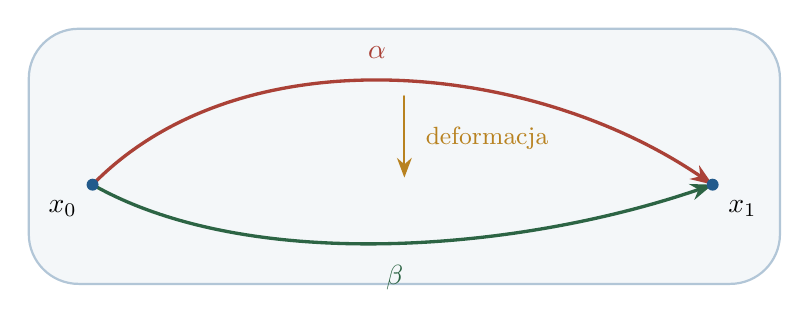
\begin{tikzpicture}[>=Stealth,line cap=round,line join=round,scale=.9]
 \fill[manifoldblue!5,rounded corners=18pt]
  (-.4,-1.15) rectangle (10.2,2.45);
 \draw[manifoldblue!35,thick,rounded corners=18pt]
  (-.4,-1.15) rectangle (10.2,2.45);
 \coordinate (x) at (.5,.25);
 \coordinate (y) at (9.25,.25);
 \draw[manifoldred,very thick,-{Stealth[length=2.8mm]}]
  (x) .. controls (2.6,2.4) and (6.7,2.0) .. (y)
  node[pos=.48,above=4pt] {$\alpha$};
 \draw[manifoldgreen!80!black,very thick,-{Stealth[length=2.8mm]}]
  (x) .. controls (2.7,-1.0) and (6.5,-.7) .. (y)
  node[pos=.51,below=4pt] {$\beta$};
 \draw[manifoldgold!90!black,thick,-{Stealth[length=2.5mm]}]
  (4.9,1.5) -- (4.9,.35)
  node[pos=.52,right=4pt,font=\small] {deformacja};
 \fill[manifoldblue] (x) circle(2.4pt) (y) circle(2.4pt);
 \node[below left=3pt] at (x) {$x_0$};
 \node[below right=3pt] at (y) {$x_1$};
\end{tikzpicture}
\caption{Homotopia dróg przesuwa ich wnętrza,
ale zachowuje oba punkty końcowe.}
\label{fig:homotopia-drog}
\end{figure}

\begin{lemat}[Zmiana prędkości nie zmienia klasy]
\label{lem:reparametr-drogi}
Jeśli $r:I\to I$ jest ciągła, niemalejąca
i spełnia $r(0)=0$, $r(1)=1$, to
$\alpha\circ r$ jest homotopijna z $\alpha$
względem końców.
\end{lemat}
\begin{proof}
Połóżmy $r_t(s)=(1-t)r(s)+ts$.
Każde $r_t$ jest ciągłe, ma te same końce
i wartości w $I$. Funkcja
$H(s,t)=\alpha(r_t(s))$ jest ciągła.
Dla $t=0$ daje $\alpha\circ r$, dla $t=1$
daje $\alpha$, a końce pozostają stałe.
\end{proof}

\begin{twierdzenie}[Grupa podstawowa]
\label{thm:grupa-podstawowa}
Klasy homotopii pętli opartych w $x_0$,
z działaniem $[\alpha][\beta]=[\alpha*\beta]$,
tworzą grupę $\pi_1(X,x_0)$.
Element neutralny to stała pętla $c_{x_0}$,
a odwrotnością $[\alpha]$ jest $[\bar\alpha]$.
\end{twierdzenie}
\begin{proof}
Jeśli $H$ deformuje $\alpha$ w $\alpha'$,
a $K$ deformuje $\beta$ w $\beta'$
względem końców, sklejenie
\[
 L(s,t)=
 \begin{cases}
   H(2s,t),&s\leq\tfrac12,\\
   K(2s-1,t),&s\geq\tfrac12
 \end{cases}
\]
jest ciągłe, bo na wspólnej krawędzi
obie części mają wartość $x_0$.
Działanie nie zależy więc od reprezentantów.

Przy trzech pętlach $(\alpha*\beta)*\gamma$
przeznacza na $\alpha,\beta,\gamma$
odcinki czasu długości $1/4,1/4,1/2$,
zaś $\alpha*(\beta*\gamma)$ długości
$1/2,1/4,1/4$. Obie drogi przebiegają
te same kawałki w tej samej kolejności
i różnią się zmianą parametru.
Lemat~\ref{lem:reparametr-drogi} daje łączność
na klasach. Pętle $c_{x_0}*\alpha$
i $\alpha*c_{x_0}$ różnią się od $\alpha$
tylko chwilą postoju, więc
$[c_{x_0}]$ jest neutralny.

Dla odwrotności określmy
\[
 H(s,t)=
 \begin{cases}
  \alpha(2(1-t)s),&0\leq s\leq\tfrac12,\\
  \alpha(2(1-t)(1-s)),&\tfrac12\leq s\leq1.
 \end{cases}
\]
Przy $s=1/2$ obie gałęzie są równe
$\alpha(1-t)$, a przy $s=0,1$ mają
wartość $x_0$. Jest to homotopia
$\alpha*\bar\alpha$ do pętli stałej
względem punktu bazowego. Zamiana
$\alpha$ z $\bar\alpha$ daje też
$[\bar\alpha][\alpha]=[c_{x_0}]$.
\end{proof}

\begin{stwierdzenie}[Odwzorowania indukowane i punkt bazowy]
\label{prop:pi1-funktor}
Odwzorowanie ciągłe $f:(X,x_0)\to(Y,y_0)$
z $f(x_0)=y_0$ wyznacza homomorfizm
\[
 f_*:\pi_1(X,x_0)\to\pi_1(Y,y_0),
 \qquad [\alpha]\mapsto[f\circ\alpha].
\]
Zachodzi $(gf)_*=g_*f_*$ i
$(\id_X)_*=\id$. Homotopia odwzorowań
utrzymująca $x_0$ w $y_0$ daje
równe homomorfizmy. Jeśli
$u$ jest drogą od $x_0$ do $x_1$,
to $b_u([\alpha])=[\bar u*\alpha*u]$
jest izomorfizmem
$\pi_1(X,x_0)\to\pi_1(X,x_1)$.
\end{stwierdzenie}
\begin{proof}
Złożenie $f\circ H$ przenosi homotopię
pętli w homotopię ich obrazów, a
$f\circ(\alpha*\beta)
=(f\circ\alpha)*(f\circ\beta)$.
Równości dla złożeń wynikają stąd wprost.
Jeśli $F$ jest homotopią odwzorowań utrzymującą
punkt bazowy, $F(\alpha(s),t)$ jest
homotopią pętli opartych w $y_0$.
Wreszcie $b_u$ zachowuje iloczyn:
w środku złożenia pojawia się
$u*\bar u$, homotopijna z pętlą stałą.
Odwrotność stanowi $b_{\bar u}$.
\end{proof}

\begin{wniosek}[Niezmienniczość grupy podstawowej]
\label{cor:pi1-homotopia}
Jeśli $f\simeq g:X\to Y$ przez homotopię
$H$, a $u(t)=H(x_0,t)$ prowadzi od
$f(x_0)$ do $g(x_0)$, to
$g_*=b_u\circ f_*$. Każda równoważność
homotopijna $f:X\to Y$ daje więc
izomorfizm grup podstawowych,
po uwzględnieniu zmiany punktu bazowego.
\end{wniosek}
\begin{proof}
Dla pętli $\alpha$ rozpatrzmy kwadrat
$(s,t)\mapsto H(\alpha(s),t)$.
Jego dolny i górny bok to $f\alpha$
i $g\alpha$, a oba pionowe boki to
$u$. Brzeg kwadratu jest homotopijny do pętli stałej względem
wybranego narożnika: w wypukłym kwadracie ściągamy jego parametryzację
liniowo do tego narożnika, a następnie składamy z $H(\alpha(s),t)$.
Zatem w grupie z punktem
bazowym $g(x_0)$ mamy
$[g\alpha]=[\bar u*(f\alpha)*u]$.
To daje pierwszą równość.

Niech teraz $g$ będzie homotopijną
odwrotnością $f$ i oznaczmy
$y_0=f(x_0)$. Homotopia
$gf\simeq\id_X$ daje drogę $u$
od $gf(x_0)$ do $x_0$ i
izomorfizm $b_u\circ(gf)_*$.
Homotopia $fg\simeq\id_Y$ daje pewną drogę $v$
od $fg(y_0)$ do $y_0$ z $b_v\circ(fg)_*=\id$.
Droga $fu$ ma te same końce, choć może nie być równa $v$.
Ponieważ $b_{fu}\circ b_v^{-1}$ jest izomorfizmem,
również $b_{fu}\circ(fg)_*$ jest izomorfizmem grupy
$\pi_1(Y,y_0)$ na siebie
(każda zmiana punktu bazowego
jest izomorfizmem).
Z naturalności konkatenacji
$f_*\circ b_u=b_{f u}\circ f_*$
na odpowiednich grupach.
Zatem dla $g'_*:=b_u\circ g_*$
oba złożenia $g'_*f_*$
oraz $f_*g'_*$ są izomorfizmami.
Pierwsze zapewnia iniektywność
$f_*$, drugie jego surjektywność.
\end{proof}

Silna retrakcja deformacyjna
z~\ref{def:retrakt-deformacyjny} daje
izomorfizm grup podstawowych w punktach
podprzestrzeni. Dla przestrzeni wypukłej
każdą pętlę $\alpha$ można deformować
wzorem $(1-t)\alpha(s)+tx_0$ do pętli
stałej, nie ruszając punktu bazowego.

\section{Nakrycia: lokalnie wiele kopii jednej przestrzeni}
\label{sec:nakrycia}

Nakrycie przypomina nałożenie kilku arkuszy
na tę samą małą okolicę. Gdy idziemy po bazie,
wybranie początkowego arkusza jednoznacznie
ustala przebieg drogi na nakryciu.
Po zamkniętej drodze możemy wrócić na inny arkusz.

\begin{definicja}[Nakrycie i arkusze]
\index{nakrycie i arkusze@Nakrycie i arkusze}
\label{def:nakrycie}
Surjekcja ciągła $p:E\to X$ jest \emph{nakryciem},
jeśli każdy $x\in X$ ma otwarte otoczenie $U$
takie, że
\[
 p^{-1}(U)=\coprod_{\lambda\in\Lambda}V_\lambda,
 \qquad
 p|_{V_\lambda}:V_\lambda\xrightarrow{\cong}U,
\]
gdzie $V_\lambda$ są parami rozłącznymi
otwartymi podzbiorami $E$, a ograniczenia $p|_{V_\lambda}$
są homeomorfizmami.
Takie $U$ nazywamy \emph{równomiernie nakrytym},
a $V_\lambda$ \emph{arkuszami}.
Włókno $p^{-1}(x)$ jest dyskretne.
\end{definicja}

\begin{przyklad}[Prosta nad okręgiem]
\label{prz:exp-nakrycie}
Odwzorowanie
\[
 p:\R\to S^1,\qquad p(t)=e^{2\pi i t},
\]
jest nakryciem. Jeśli $U$ jest krótkim,
otwartym łukiem okręgu, wybierzmy przedział
$J$ długości mniejszej niż $1$, na którym
$p|_J$ jest homeomorfizmem na $U$.
Wtedy $p^{-1}(U)=\coprod_{k\in\Z}(J+k)$.
Włókno nad $1$ to $\Z$.
Podobnie $q_m:S^1\to S^1$, $q_m(z)=z^m$,
jest $m$-krotnym nakryciem dla $m\geq1$.
Dwukrotne nakrycie $\operatorname{Spin}(n)
\to\mathrm{SO}(n)$ pojawiło się już w
Twierdzeniu~\ref{thm:spin-nakrycie}.
\end{przyklad}

\begin{figure}[!htbp]
\centering
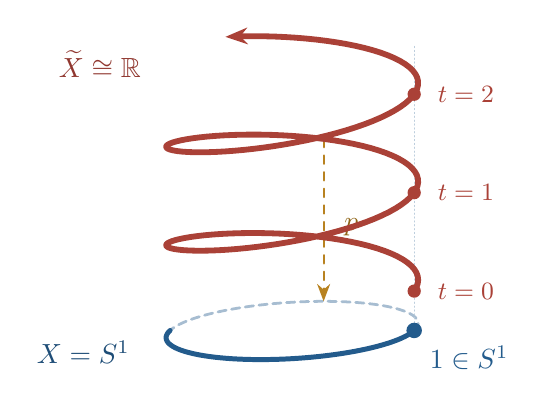
\begin{tikzpicture}[>=Stealth,line cap=round,line join=round,
 x={(1.55cm,0cm)},y={(.40cm,.37cm)},z={(0cm,1.25cm)}]
 % Okrąg u dołu, widoczna i zasłonięta połowa.
 \draw[manifoldblue!40,densely dashed,line width=1pt]
  plot[domain=0:180,samples=60,variable=\u]
   ({cos(\u)},{sin(\u)},0);
 \draw[manifoldblue,line width=1.8pt]
  plot[domain=180:360,samples=60,variable=\u]
   ({cos(\u)},{sin(\u)},0);
 % Włókno nad 1 oraz promień projekcji dla punktu t=1.25.
 \draw[manifoldblue!30,densely dotted]
  (1,0,0)--(1,0,2.9);
 \draw[manifoldgold!90!black,thick,dashed,
       -{Stealth[length=2.2mm]}]
  (0,1,1.65)--(0,1,0);
 \node[manifoldgold!70!black,right=4pt]
  at (0,1,.75) {$p$};
 % Fragment helisy: jeden obrót podnosi wysokość o jedną jednostkę.
 \draw[manifoldred,line width=2.1pt,
       -{Stealth[length=2.8mm]}]
  plot[domain=0:2.38,samples=180,variable=\t]
   ({cos(360*\t)},{sin(360*\t)},{.4+\t});
 \foreach \k in {0,1,2} {
  \fill[manifoldred] (1,0,{.4+\k}) circle(2.4pt);
  \node[manifoldred,right=5pt,font=\small]
   at (1,0,{.4+\k}) {$t=\k$};
 }
 \fill[manifoldblue] (1,0,0) circle(2.8pt);
 \node[manifoldblue,below right=3pt] at (1,0,0) {$1\in S^1$};
 \node[manifoldred!85!black,left=7pt]
  at (-1,0,2.7) {$\widetilde X\cong\R$};
 \node[manifoldblue!85!black,left=11pt]
  at (-1,0,-.22) {$X=S^1$};
\end{tikzpicture}
\caption{Nakrycie $p:\R\to S^1$, $p(t)=e^{2\pi i t}$,
przedstawione jako linia śrubowa nad okręgiem. Rzut pionowy
odpowiada $p$. Punkty linii śrubowej oznaczone $t=0,1,2$
leżą nad tym samym punktem $1\in S^1$.
Pokazano fragment linii śrubowej, która biegnie dalej
w obie strony.}
\label{fig:nakrycie-okragu}
\end{figure}

W poniższych dowodach użyjemy \emph{liczby Lebesgue'a}:
dla otwartego pokrycia zwartej przestrzeni metrycznej istnieje
$\delta>0$ takie, że każdy niepusty zbiór o średnicy mniejszej
niż $\delta$ leży w jednym elemencie pokrycia.
Oto uzasadnienie. Dla każdego $x$ wybierzmy $\varepsilon_x>0$
tak, aby $B(x,2\varepsilon_x)$ mieściła się w elemencie pokrycia.
Ze zwartości skończenie wiele kul $B(x_i,\varepsilon_{x_i})$
pokrywa przestrzeń. Wystarczy $\delta=\min_i\varepsilon_{x_i}$:
jeśli $y$ należy do jednej z tych mniejszych kul, wszystkie
punkty zbioru zawierającego $y$ i o średnicy $<\delta$
leżą w odpowiadającej jej większej kuli. Stosujemy ten fakt
do odcinka i kwadratu z ich zwykłą metryką.

\begin{twierdzenie}[Podnoszenie drogi i homotopii]
\label{thm:podnoszenie-nakrycie}
Niech $p:E\to X$ będzie nakryciem.
\begin{enumerate}[label=(\alph*),leftmargin=*]
\item Każda droga $\gamma:I\to X$ i wybór
      $e_0\in p^{-1}(\gamma(0))$ wyznaczają
      dokładnie jedną drogę
      $\widetilde\gamma:I\to E$ z
      $\widetilde\gamma(0)=e_0$ i
      $p\widetilde\gamma=\gamma$.
\item Jeśli $H:I\times I\to X$ jest
      homotopią dróg, a $\widetilde H(s,0)$
      jest zadanym podniesieniem $H(s,0)$,
      to istnieje dokładnie jedno ciągłe
      podniesienie $\widetilde H$ całego $H$.
      Gdy $H$ zachowuje końce dróg,
      podniesione końce również są stałe.
\end{enumerate}
\end{twierdzenie}
\begin{proof}
\emph{Droga.} Przeciwobrazy równomiernie
nakrytych otwartych $U$ tworzą otwarte
pokrycie odcinka $I$. Z liczby Lebesgue'a
tego pokrycia wybieramy podział
$0=t_0<\cdots<t_N=1$ tak drobny, aby
każdy obraz $\gamma([t_{j-1},t_j])$
mieścił się w jednym $U_j$.
Arkusz nad $U_1$ zawierający $e_0$
określa na pierwszym przedziale wzór
\[
 \widetilde\gamma(t)
 =(p|_{V_1})^{-1}(\gamma(t)).
\]
W punkcie $t_1$ wybieramy arkusz nad $U_2$
zawierający uzyskany punkt włókna i powtarzamy.
Wzory zgadzają się na końcach przedziałów,
więc sklejają się w drogę ciągłą.
Jeśli dwa podniesienia zgadzają się w pewnej
chwili, to lokalnie leżą w tym samym arkuszu
i są identyczne. Gdy w pewnej chwili
się różnią, leżą nad tym samym punktem
w różnych arkuszach, więc również w małej
okolicy chwili pozostają różne. Zbiór
chwil zgodności jest zatem otwarty
i domknięty w spójnym $I$ oraz
zawiera $0$, co daje jednoznaczność.

\emph{Homotopia.} Pokrycie $I^2$ zbiorami
$H^{-1}(U)$ ma liczbę Lebesgue'a.
Dzielimy kwadrat na skończoną siatkę
małych prostokątów, z których każdy ma
obraz w jednym równomiernie nakrytym $U$.
Na dolnej krawędzi mamy zadaną drogę.
Podnosimy prostokąty kolejno od dołu i
od lewej: na każdym wybieramy arkusz
zawierający już ustalony obraz jego narożnika
i stosujemy $(p|_V)^{-1}\circ H$.
Na wspólnej krawędzi oba wzory są
podniesieniami tej samej drogi i zgadzają
się w narożniku, więc na mocy (a) są równe.
Skończone sklejanie daje ciągłą
$\widetilde H$; lokalna jednoznaczność
na spójnym $I^2$ daje jej jedyność.
Jeśli $H(0,t)$ albo $H(1,t)$ jest stała,
jej podniesienie leży w dyskretnym włóknie,
więc też jest stałe.
\end{proof}

Stąd $p_*:\pi_1(E,e_0)\to\pi_1(X,p(e_0))$
jest iniektywny. Jeśli obraz pętli jest
homotopijny do stałej pętli względem bazy,
podnosimy homotopię od danej pętli w $E$.
Końcowa podniesiona pętla leży w dyskretnym
włóknie i jest stała.

\begin{twierdzenie}[Kryterium podnoszenia odwzorowań]
\label{thm:kryterium-podnoszenia}
Niech $Y$ będzie łukowo spójna i lokalnie
łukowo spójna, $f:Y\to X$ ciągła,
$p:E\to X$ nakryciem, a $p(e_0)=f(y_0)$.
Istnieje ciągła $\widetilde f:Y\to E$
z $p\widetilde f=f$ i
$\widetilde f(y_0)=e_0$ wtedy i tylko wtedy, gdy
\[
 f_*\pi_1(Y,y_0)\subseteq
 p_*\pi_1(E,e_0).
\]
Takie podniesienie jest jedyne.
\end{twierdzenie}
\begin{proof}
Gdy $\widetilde f$ istnieje,
$f=p\widetilde f$, zatem
$f_*=p_*\widetilde f_*$, co daje konieczność.
Załóżmy inkluzję. Dla $y\in Y$ wybierzmy
drogę $\gamma$ od $y_0$ do $y$ i
zdefiniujmy $\widetilde f(y)$ jako koniec
podniesienia $f\circ\gamma$ z początkiem $e_0$.
Gdy $\gamma'$ jest innym wyborem,
pętla $f\circ(\gamma'*\bar\gamma)$
ma klasę w obrazie $p_*$. Jest więc
homotopijna względem punktu bazowego
do obrazu pewnej pętli w $E$ o początku
$e_0$. Podnosząc tę homotopię za pomocą
Twierdzenia~\ref{thm:podnoszenie-nakrycie},
otrzymujemy, że podniesienie
$f\circ(\gamma'*\bar\gamma)$ wraca do $e_0$.
Druga część tego zamkniętego podniesienia jest podniesieniem
$f\circ\bar\gamma$ kończącym się w $e_0$.
Po odwróceniu jest, z jednoznaczności, podniesieniem
$f\circ\gamma$ zaczynającym się w $e_0$.
Podniesienia $f\circ\gamma$ i $f\circ\gamma'$ mają więc ten sam koniec.

Sprawdźmy ciągłość, której nie daje sama
definicja punkt po punkcie. Wybierzmy
równomiernie nakryte $U$ zawierające $f(y)$
oraz łukowo spójne otwarte $W\ni y$ z
$f(W)\subseteq U$. Niech $V$ będzie
arkuszem nad $U$ zawierającym $\widetilde f(y)$.
Dla $z\in W$ połączmy $y$ z $z$ drogą
w $W$ i dopiszmy ją do drogi od $y_0$
do $y$. Definicja i podnoszenie drogi
pokazują wtedy, że
$\widetilde f(z)=(p|_V)^{-1}(f(z))$.
Na $W$ odwzorowanie jest więc ciągłe.
Jedyność wynika z jedyności podniesienia
każdej drogi od $y_0$.
\end{proof}

\begin{twierdzenie}[Grupa podstawowa okręgu]
\label{thm:pi1-okragu}
Podnoszenie względem $p:\R\to S^1$
z Przykładu~\ref{prz:exp-nakrycie} daje
izomorfizm
\[
 \operatorname{wind}:\pi_1(S^1,1)\xrightarrow{\ \cong\ }\Z,
 \qquad [\gamma]\longmapsto
 \widetilde\gamma(1),
 \quad \widetilde\gamma(0)=0.
\]
Liczba po prawej to \emph{liczba owinięć}.
\end{twierdzenie}
\begin{proof}
Ponieważ $\gamma(1)=1$, koniec
podniesienia leży w $p^{-1}(1)=\Z$.
Homotopijne pętle dają homotopię
podniesień z nieruchomymi końcami,
więc liczba zależy tylko od klasy.
Jeśli podniesienie $\alpha$ kończy się w $k$,
to podniesienie następnej pętli $\beta$
zaczynające się w $k$ jest przesunięciem
o $k$ podniesienia zaczynającego się w $0$.
Stąd $\operatorname{wind}([\alpha*\beta])
=\operatorname{wind}([\alpha])
+\operatorname{wind}([\beta])$.
Pętla $\gamma_k(s)=e^{2\pi i ks}$
ma podniesienie $ks$, więc homomorfizm
jest surjektywny. Gdy podniesienie
$\widetilde\gamma$ wraca do $0$,
wzór $(s,t)\mapsto(1-t)\widetilde\gamma(s)$
deformuje ją w $\R$ do stałej drogi
z zachowaniem końców. Projekcja tej
homotopii do $S^1$ deformuje $\gamma$
do pętli stałej. Jądro jest zerowe.
\end{proof}

Z Przykładu~\ref{prz:retrakcja-pierscien}
otrzymujemy $\pi_1(\R^2\setminus\{0\})\cong\Z$.
W szczególności okrąg i punkt nie są
homotopijnie równoważne. Obliczenie
$\pi_1(S^{n})=0$ dla $n\geq2$
wyniknie niżej z twierdzenia van Kampena.

\begin{definicja}[Lokalna spójność i warunek półlokalny]
\index{lokalna spojnosc i warunek pollokalny@Lokalna spójność i warunek półlokalny}
\label{def:semilokalnie-prosto-spojna}
Przestrzeń $X$ jest \emph{lokalnie łukowo spójna},
gdy każdy punkt ma bazę otoczeń otwartych,
które są łukowo spójne. Jest
\emph{półlokalnie jednospójna}, gdy każdy
$x\in X$ ma otoczenie $U$, w którym
każda pętla oparta w $x$ jest homotopijna do stałej
względem punktu bazowego \emph{w całym $X$}. Nie wymagamy, aby
ta homotopia mieściła się w $U$.
Przestrzeń łukowo spójna z
$\pi_1(X,x_0)=0$ jest \emph{jednospójna}.
\end{definicja}

Każda rozmaitość topologiczna spełnia
lokalne warunki z tej definicji, gdyż
w otwartej mapie współrzędnych można
wybrać małą kulę. Warunek półlokalny
jest ważny: bez niego nakrycie uniwersalne
może w ogóle nie istnieć.

\begin{twierdzenie}[Konstrukcja nakrycia uniwersalnego]
\label{thm:uniwersalne-nakrycie}
Jeśli $X$ jest łukowo spójna, lokalnie
łukowo spójna i półlokalnie jednospójna,
to ma nakrycie $q:\widetilde X\to X$
z jednospójną przestrzenią $\widetilde X$.
\end{twierdzenie}
\begin{proof}
Ustalmy $x_0\in X$. Punktem $\widetilde X$
niech będzie klasa $[\gamma]$ drogi w $X$
zaczynającej się w $x_0$, przy czym
homotopie zachowują oba końce.
Definiujemy $q([\gamma])=\gamma(1)$.
Istnieje baza otwartych łukowo spójnych
zbiorów $U\subseteq X$, w których
każda pętla jest zerowa po włączeniu do $X$:
najpierw wybieramy otoczenie z warunku
półlokalnego, następnie w nim małe
łukowo spójne otoczenie z lokalnej
łukowej spójności. Każdą pętlę opartą w innym punkcie
takiego $U$ przenosimy do jego wyróżnionego punktu drogą w $U$;
izomorfizm zmiany punktu bazowego pokazuje, że ona też jest zerowa w $X$.

Dla drogi $\gamma$ kończącej się w $x\in U$
niech $W([\gamma],U)$ składa się z klas
$[\gamma*\eta]$, gdzie $\eta$ jest drogą
w $U$ od $x$ do dowolnego $y\in U$.
Jeśli dwie takie drogi $\eta,\eta'$
mają ten sam koniec, to
$\eta*\bar\eta'$ jest pętlą w $U$,
zerową w $X$. Zatem $[\gamma*\eta]
=[\gamma*\eta']$. Otrzymujemy bijekcję
$q:W([\gamma],U)\to U$. Bierzemy wszystkie
te zbiory jako bazę topologii. Sprawdźmy warunek przecięć:
jeśli $[\beta]\in W([\gamma],U)\cap W([\gamma'],U')$,
wybieramy otwarte łukowo spójne $O$ z naszej bazy,
zawierające $\beta(1)$ i zawarte w $U\cap U'$.
Wtedy $W([\beta],O)$ zawiera $[\beta]$ i mieści się w obu zbiorach:
do drogi kończącej się w $\beta(1)$ dopisujemy tylko drogę w $O$.
To dowodzi, że rzeczywiście otrzymujemy bazę.
Ograniczenie $q$ do każdego $W$ jest ciągłe, ponieważ przeciwobrazy
otwartych podzbiorów $U$ są sumami takich mniejszych zbiorów bazowych;
jest też otwarte, bo mniejsze $W([\beta],O)$ przechodzą na otwarte $O$.
Wcześniej wykazana bijekcja jest więc homeomorfizmem.
Jeśli dwa $W$ nad tym samym
$U$ mają wspólny punkt, ich drogi początkowe
różnią się drogą w $U$ z dokładnością
do homotopii w $X$, więc zbiory $W$
są równe. Dla mniejszych otoczeń
używamy ograniczenia tych samych odwzorowań.
Stąd $q^{-1}(U)$ jest rozłączną sumą
arkuszy $W([\gamma],U)$: $q$ jest nakryciem.

Jest ono łukowo spójne. Drogę od klasy
stałej $[c_{x_0}]$ do $[\gamma]$
otrzymujemy, biorąc po kolei klasy
odcinków $\gamma|_{[0,t]}$ po
przeparametryzowaniu na $I$; lokalnie
leżą one w jednym $W$, więc tworzą
ciągłą drogę. Jeśli pętla
$\lambda$ w $\widetilde X$ jest oparta
w $[c_{x_0}]$, jej rzut $\gamma=q\lambda$
ma podniesienie $\lambda$ i kończy
się w tej samej klasie drogi.
Konstrukcja podniesienia pokazuje,
że ta klasa jest $[\gamma]$, więc
$\gamma$ jest homotopijna do stałej
pętli względem bazowego końca.
Podnosimy tę homotopię, zaczynając
od $\lambda$, za pomocą
Twierdzenia~\ref{thm:podnoszenie-nakrycie}.
Na końcu dostajemy stałą pętlę
w dyskretnym włóknie. Zatem
$\pi_1(\widetilde X)=0$.
\end{proof}

\begin{uwaga}[Skąd podgrupy grupy podstawowej?]
\label{uwaga:nakrycia-podgrupy}
Dla spójnego nakrycia $p:(E,e_0)\to(X,x_0)$
iniekcja $p_*$ wyróżnia podgrupę
$H=p_*\pi_1(E,e_0)\leq\pi_1(X,x_0)$.
W warunkach Twierdzenia~\ref{thm:uniwersalne-nakrycie}
każda taka podgrupa daje nakrycie:
na klasach dróg w $\widetilde X$ grupa
$\pi_1(X,x_0)$ działa przez
$[\omega]\cdot[\gamma]=[\omega*\gamma]$,
a iloraz $H\backslash\widetilde X$
jest nakryciem $X$. Istotnie, działanie przenosi
$W([\gamma],U)$ na $W([\omega*\gamma],U)$,
więc jest działaniem przez homeomorfizmy. Jest wolne:
z $[\omega*\gamma]=[\gamma]$ po dopisaniu $\bar\gamma$
wynika $[\omega]=1$.
Co więcej, jeśli $hW\cap W\ne\varnothing$, to $hW=W$,
bo są to arkusze nad tym samym $U$. Ponieważ $q$ jest
iniektywne na $W$ i $q(hz)=q(z)$, element $h$ ustala punkt $z\in W$;
stąd $h=1$. Różne przesunięcia jednego arkusza są więc rozłączne.
Projekcja na orbity jest otwarta: przeciwobraz obrazu zbioru
otwartego $O$ jest sumą otwartych zbiorów $hO$.
Obrazy arkuszy w ilorazie są zatem otwarte i każdy odwzorowuje się
homeomorficznie na $U$. To uzasadnia własność nakrycia.
Przestrzeń ilorazowa jest łukowo spójna jako obraz $\widetilde X$.
Podniesienie pętli $\gamma$ z $x_0$ kończy się w orbicie $[\gamma]$;
wraca do orbity drogi stałej dokładnie wtedy, gdy $[\gamma]\in H$.
Ponieważ obraz homomorfizmu indukowanego przez nakrycie składa się
właśnie z klas mających zamknięte podniesienie, skonstruowane nakrycie
realizuje dokładnie podgrupę $H$.
Z drugiej strony kryterium
\ref{thm:kryterium-podnoszenia} podnosi
$q:\widetilde X\to X$ do $E$, z ustaloną wartością $e_0$.
Przy obecnych założeniach $E$ jest lokalnie łukowo spójna,
więc jej spójność daje łukową spójność: składowe łukowe są otwarte.
Każdy punkt $E$ można połączyć z $e_0$ drogą; rzut tej drogi
pokazuje, że podniesione odwzorowanie $\widetilde X\to E$ jest surjektywne.
Dwa punkty $[\gamma],[\gamma']$ nad tym samym punktem $X$
trafiają w ten sam punkt $E$
dokładnie wtedy, gdy $[\gamma'*\bar\gamma]\in H$.
W jedną stronę składamy podniesione drogi o wspólnym końcu,
otrzymując pętlę w $E$; w drugą używamy podnoszenia homotopii
jak w dowodzie kryterium podnoszenia. Ten warunek jest też
równoważny przynależności do jednej orbity, gdyż
$[\gamma'*\bar\gamma]\cdot[\gamma]=[\gamma']$.
Lokalnie obie projekcje są
homeomorfizmami na $U$, co daje
$E\cong H\backslash\widetilde X$
nad $X$. Zmiana wybranego punktu
$e_0$ sprzęga podgrupę $H$: droga w $E$ między dwoma punktami
nad $x_0$ rzutuje się na pętlę $u$, a zmiana bazy zastępuje
$H$ podgrupą $[\bar u]H[u]$.
Odwrotnie, dowolną pętlę $u$ w $X$ można podnieść z $e_0$;
jej koniec wybiera punkt włókna realizujący właśnie to sprzężenie.
Tak powstaje klasyfikacja spójnych
nakryć przez klasy sprzężoności
podgrup $\pi_1(X,x_0)$.
\end{uwaga}

\section{Twierdzenie van Kampena i pierwsze obliczenia}
\label{sec:van-kampen}

Nakrycie okręgu mierzy jedną liczbę owinięć.
Gdy przestrzeń składa się z kilku części,
potrzebujemy sposobu łączenia informacji
o pętlach w tych częściach.

\begin{twierdzenie}[van Kampen: dwa otwarte zbiory]
\label{thm:van-kampen}
Niech $X=U\cup V$, gdzie $U,V$ są otwarte,
łukowo spójne, a $U\cap V$ jest łukowo
spójne i zawiera $x_0$. Jeśli
$G_U=\pi_1(U,x_0)$, $G_V=\pi_1(V,x_0)$
oraz $G_0=\pi_1(U\cap V,x_0)$, to
\[
 \pi_1(X,x_0)\cong
 (G_U*G_V)/
 \left\langle\!\left\langle
 (i_U)_*(h)(i_V)_*(h)^{-1}:h\in G_0
 \right\rangle\!\right\rangle.
\]
Iloczyn wolny i redukcję słów wyjaśnia
Definicja~\ref{def:free-groups-5}, a zapis
$\langle\!\langle\cdot\rangle\!\rangle$
oznacza domknięcie normalne z
Definicji~\ref{def:normal-quotient-5}.
\end{twierdzenie}
\begin{proof}
Włączenia $U,V\hookrightarrow X$
określają homomorfizm
$\Phi:G_U*G_V\to\pi_1(X,x_0)$.
Pętla w $U\cap V$ daje ten sam obraz
niezależnie od wyboru strony.
Zatem wszystkie relacje z tezy
leżą w $\ker\Phi$.

\emph{Surjektywność.} Dla pętli
$\alpha:I\to X$ przeciwobrazy $U,V$
pokrywają zwarty odcinek. Dzielimy
go na tyle małych przedziałów,
aby obraz każdego leżał w $U$ albo $V$.
Sąsiednie kawałki przypisane temu
samemu zbiorowi łączymy. Każdy
punkt przejścia między kawałkiem
w $U$ i kawałkiem w $V$ leży w
$U\cap V$. Łączymy go z $x_0$
pomocniczą drogą w $U\cap V$.
Jeśli $\lambda_j$ prowadzi od $x_0$
do $j$-tego punktu przejścia,
to z kawałka $\alpha_j$ budujemy
pętlę $\lambda_{j-1}*\alpha_j*
\bar\lambda_j$ całkowicie w $U$
albo w $V$. Iloczyn tych pętli
odtwarza $\alpha$: sąsiednie
$\bar\lambda_j*\lambda_j$
kasują się na mocy
Twierdzenia~\ref{thm:grupa-podstawowa}.

Zmiana drogi $\lambda_j$ na $\lambda'_j$
wyznacza pętlę $h=\lambda'_j*\bar\lambda_j$ w $U\cap V$
\emph{opartą w $x_0$}. Poprzedni czynnik słowa mnożymy z prawej
przez $h^{-1}$, a następny z lewej przez $h$.
Oba zapisy $h$ są równe w ilorazie z tezy, więc się skracają.
Również dopisanie podziału wewnątrz
jednego otwartego zbioru nie zmienia
otrzymanej klasy słowa.

\emph{Jądro.} Przypuśćmy, że słowo
z $G_U*G_V$ daje pętlę homotopijną
do stałej w $X$. Wypełnijmy ją
homotopią $F:I^2\to X$, stałą na
pozostałych trzech bokach.
Zwartość kwadratu pozwala wybrać
siatkę tak drobną, by obraz
każdego małego prostokąta leżał
w całości w $U$ lub w $V$.
Podział dolnego boku dobieramy także tak, aby zawierał końce
pętli reprezentujących litery wyjściowego słowa.
Dla każdego wierzchołka $z$ siatki wybierzmy drogę $\mu_z$
od $x_0$ do $F(z)$. Jeśli $F(z)\in U\cap V$, wybieramy ją
w przecięciu; jeśli $F(z)$ należy tylko do jednego zbioru,
wybieramy drogę w tym zbiorze. Jest to możliwe dzięki założeniom
o łukowej spójności. Przy $F(z)=x_0$ wybieramy drogę stałą.

Zorientowanej krawędzi $e:z\to w$ przypisujemy klasę
$[\mu_z*(F|_e)*\bar\mu_w]$ w grupie zbioru zawierającego
obraz sąsiedniego prostokąta. Obie drogi pomocnicze leżą w tym
zbiorze. Jeżeli dwa sąsiednie prostokąty mają różne oznaczenia,
ich wspólna krawędź i obie drogi pomocnicze leżą w $U\cap V$,
więc przypisania dają ten sam element ilorazu z tezy.
Odwrócenie krawędzi daje element odwrotny.

Iloczyn czterech elementów wokół jednego prostokąta jest jedynką:
drogi pomocnicze skracają się parami, a jego brzeg jest homotopijny
do stałej we właściwym $U$ lub $V$, przez mapę $F$ na tym prostokącie.
Możemy zatem zastępować dwa kolejne boki prostokąta pozostałymi
dwoma, z tymi samymi końcami, bez zmiany elementu ilorazu.
Przesuwając tak łamaną po kolejnych prostokątach, wiersz po wierszu,
zamieniamy dolny bok kwadratu na drogę wzdłuż pozostałych trzech boków.
Te trzy boki są stałe. Na dolnym boku drogi pomocnicze wewnątrz
każdej pierwotnej litery skracają się w jej grupie, a przy końcach
liter są stałe. Odtwarzamy więc dokładnie wyjściowe słowo,
które okazało się jedynką w ilorazie. Każdy krok używał tylko
relacji wewnątrz obu grup i relacji pochodzących z przecięcia.
Stąd $\ker\Phi$ zawiera się w
wskazanym domknięciu normalnym relacji, co kończy dowód.
\end{proof}

\begin{przyklad}[Dwa okręgi złączone w punkcie]
\label{prz:pi1-dwa-okregi}
Niech $X=S^1_a\vee S^1_b$.
Wybierzmy na każdym okręgu po jednym
punkcie różnym od punktu sklejenia
$x_0$. Usuwając punkt z drugiego
okręgu, otrzymujemy otwarty $U$
retrakcyjny na $S^1_a$; analogicznie
$V$ retrakcyjny na $S^1_b$.
Przecięcie $U\cap V$ jest ściągalne
(to dwa otwarte łuki spotykające się
w $x_0$). Wobec tego
\[
 \pi_1(S^1\vee S^1,x_0)
 \cong\Z*\Z=:F(a,b).
\]
Słowa $ab$ i $ba$ są różne:
grupa podstawowa nie musi być przemienna.
\end{przyklad}

\begin{przyklad}[Sfera wymiaru co najmniej dwa]
\label{prz:pi1-sfera}
Niech $n\geq2$. Zbiory
$U=S^n\setminus\{N\}$ i
$V=S^n\setminus\{S\}$, gdzie $N,S$
są biegunami, są homeomorficzne
z $\R^n$, więc mają trywialne
grupy podstawowe. Ich przecięcie
jest łukowo spójne: deformuje się
na równik $S^{n-1}$, który jest
łukowo spójny dla $n-1\geq1$.
Twierdzenie~\ref{thm:van-kampen}
daje $\pi_1(S^n)=0$.
Stąd $\pi_1(\R^{n+1}\setminus\{0\})=0$
dla $n\geq2$, co odróżnia ten
przypadek od płaszczyzny.
\end{przyklad}

\section{Sympleksy i triangulacje}
\label{sec:sympleksy}

Sympleks jest najprostszym wielowymiarowym
klockiem: odcinek w wymiarze $1$, trójkąt
w wymiarze $2$, czworościan w wymiarze $3$.
Współrzędne barycentryczne opisują
zarazem punkt i to, na której ścianie leży.

\begin{definicja}[Sympleks standardowy i ściany]
\index{sympleks standardowy i sciany@Sympleks standardowy i ściany}
\label{def:sympleks-standardowy}
Dla $n\geq0$ \emph{standardowy $n$-sympleks}
to
\[
 \Delta^n=
 \left\{(t_0,\ldots,t_n)\in\R^{n+1}:
 t_i\geq0,\ \sum_{i=0}^{n}t_i=1\right\}.
\]
Jego wierzchołki to wektory $e_0,\ldots,e_n$.
\emph{Wnętrze} oznacza $t_i>0$ dla wszystkich $i$
(względem afinicznej otoczki sympleksu).
Dla $n\geq1$ \emph{ściana kowymiaru jeden} naprzeciw $e_i$
jest zadana równaniem $t_i=0$ i jest kopią $\Delta^{n-1}$.
Ogólniej ścianę wyznacza dowolny niepusty podzbiór wierzchołków;
jest właściwa, gdy pomija choć jeden z nich.
Suma wszystkich właściwych ścian to $\partial\Delta^n$.
Przy $n=0$ nie ma niepustych właściwych ścian i $\partial\Delta^0=\varnothing$.
Punkty $v_0,\ldots,v_n\in\R^N$
są \emph{afinicznie niezależne}, jeśli
$v_1-v_0,\ldots,v_n-v_0$ są liniowo
niezależne. Ich otoczka wypukła
$[v_0,\ldots,v_n]$ jest
\emph{geometrycznym $n$-sympleksem}.
\end{definicja}

Każdy punkt sympleksu ma postać
$x=\sum_i t_iv_i$. Współczynniki
$t_i$ są jednoznaczne: jeśli
$\sum_i(t_i-s_i)v_i=0$ i obie sumy
współczynników są równe $1$, to
$\sum_{i=1}^n(t_i-s_i)(v_i-v_0)=0$;
afiniczna niezależność wymusza
$t_i=s_i$ dla wszystkich $i$.
W szczególności usunięcie jednego
wierzchołka daje ścianę
o wymiarze $n-1$.

\begin{figure}[!htbp]
\centering
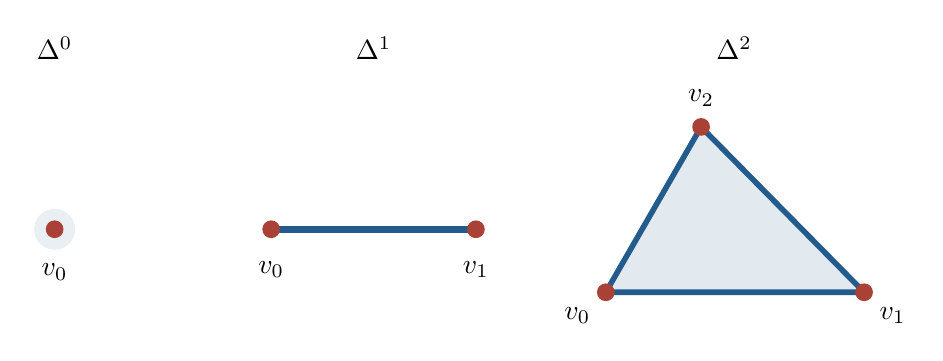
\begin{tikzpicture}[line cap=round,line join=round]
 \node[font=\bfseries] at (0,3.45) {$\Delta^0$};
 \node[font=\bfseries] at (4.05,3.45) {$\Delta^1$};
 \node[font=\bfseries] at (8.63,3.45) {$\Delta^2$};
 % Wymiar zero.
 \fill[manifoldblue!10] (0,1.15) circle(.26);
 \fill[manifoldred] (0,1.15) circle(3.2pt);
 \node[below=9pt] at (0,1.15) {$v_0$};
 % Wymiar jeden.
 \coordinate (b0) at (2.75,1.15);
 \coordinate (b1) at (5.35,1.15);
 \draw[manifoldblue,line width=2.6pt] (b0)--(b1);
 \fill[manifoldred] (b0) circle(3.2pt)
  (b1) circle(3.2pt);
 \node[below=8pt] at (b0) {$v_0$};
 \node[below=8pt] at (b1) {$v_1$};
 % Wymiar dwa.
 \coordinate (c0) at (7.00,.35);
 \coordinate (c1) at (10.28,.35);
 \coordinate (c2) at (8.21,2.45);
 \fill[manifoldblue!13] (c0)--(c1)--(c2)--cycle;
 \draw[manifoldblue,line width=2pt] (c0)--(c1)--(c2)--cycle;
 \fill[manifoldred] (c0) circle(3.2pt)
  (c1) circle(3.2pt) (c2) circle(3.2pt);
 \node[below left=3pt] at (c0) {$v_0$};
 \node[below right=3pt] at (c1) {$v_1$};
 \node[above=4pt] at (c2) {$v_2$};
\end{tikzpicture}
\caption{Sympleksy wymiarów $0,1,2$: punkt,
odcinek i wypełniony trójkąt. Wymiar
$n$ odpowiada $n+1$ afinicznie niezależnym
wierzchołkom; ściany powstają przez ich usunięcie.}
\label{fig:sympleks-trojkat}
\end{figure}

\begin{stwierdzenie}[Brzeg sympleksu jest sferą]
\label{prop:brzeg-sympleksu}
Dla $n\geq1$ przestrzeń $\Delta^n$
jest homeomorficzna z dyskiem $D^n$,
a $\partial\Delta^n$ z $S^{n-1}$.
\end{stwierdzenie}
\begin{proof}
Pracujemy w $n$-wymiarowej płaszczyźnie
afinicznej $P=\{\sum t_i=1\}$.
Środek $c=(1/(n+1),\ldots,1/(n+1))$
leży we wnętrzu. Każdy promień z $c$
w $P$ przecina brzeg dokładnie raz:
nierówności $t_i\geq0$ wyznaczają
na nim odcinek od $c$ do pierwszej
ściany, na której pewna współrzędna
staje się zerem.
Przypisanie punktowi brzegowemu
$x$ kierunku $(x-c)/\|x-c\|$
jest ciągłą bijekcją
$\partial\Delta^n\to S^{n-1}$
po utożsamieniu $P-c\cong\R^n$.
Dziedzina jest zwarta, a sfera
Hausdorffa, więc odwrotność jest
ciągła. Jeśli $b(u)$ jest tą odwrotnością dla kierunku
$u\in S^{n-1}$, wzór $ru\mapsto c+r(b(u)-c)$, $0<r\leq1$,
z wartością $c$ w zerze daje ciągłą bijekcję z $D^n$ na $\Delta^n$.
Ciągłość w zerze wynika z ograniczoności $b(u)-c$.
Ponownie zwartość i własność Hausdorffa dają homeomorfizm,
który na brzegu jest poprzednią identyfikacją. Dla $n=1$ brzeg
składa się z dwóch punktów,
czyli jest $S^0$.
\end{proof}

\begin{definicja}[Skończony kompleks symplicjalny]
\index{skonczony kompleks symplicjalny@Skończony kompleks symplicjalny}
\label{def:kompleks-symplicjalny}
Niech $V$ będzie skończonym zbiorem
wierzchołków. \emph{Kompleks symplicjalny}
$K$ to rodzina niepustych skończonych
podzbiorów $V$ taka, że jeśli
$\sigma\in K$ i $\varnothing\ne\tau\subseteq\sigma$,
to $\tau\in K$. Zbiór o $n+1$
wierzchołkach nazywamy
\emph{$n$-sympleksem} $K$.
Jego \emph{realizacja geometryczna} to
\[
 |K|=\left\{\sum_{v\in V}t_v e_v:
 t_v\geq0,\ \sum_v t_v=1,\
 \{v:t_v>0\}\in K\right\}\subseteq\R^{V}.
\]
Kompleks $L\subseteq K$ zamknięty
na przechodzenie do ścian jest
\emph{podkompleksem}.
\emph{Skończona triangulacja} przestrzeni $X$
to homeomorfizm $|K|\to X$. W tej sekcji ograniczamy się do
skończonych kompleksów; ich realizacje są zwarte. Triangulacje
przestrzeni niezwartych wymagają dopuszczenia nieskończenie wielu sympleksów.
\end{definicja}

W tej definicji dwie różne ściany
mają dokładnie to wspólne, co
wynika ze wspólnych wierzchołków.
Na przykład trzy krawędzie
$[v_0,v_1]$, $[v_1,v_2]$,
$[v_2,v_0]$, bez wnętrza trójkąta,
realizują okrąg. Po dodaniu
$[v_0,v_1,v_2]$ otrzymujemy dysk.
Słowo \emph{podkompleks} jest
ważniejsze niż dowolny podzbiór:
zawiera wraz z sympleksem
wszystkie jego ściany.

\begin{uwaga}[Nie każdy podział na trójkąty
jest kompleksem symplicjalnym]
\label{uwaga:delta-motywacja}
Kwadrat z utożsamionymi przeciwległymi
bokami przedstawia torus. Gdy podzielimy
go jedną przekątną, po sklejeniu wszystkie
cztery narożniki stają się jednym
wierzchołkiem, a każda z dwóch
trójkątnych części nadal ma sens.
Nie jest to \emph{kompleks symplicjalny}
z jednym wierzchołkiem: trójkąt
potrzebuje trzech różnych wierzchołków.
Wygodniejszym opisem są
$\Delta$-kompleksy.
\end{uwaga}

\begin{definicja}[$\Delta$-kompleks]
\label{def:delta-kompleks}
\emph{$\Delta$-kompleks} $X$ jest
przestrzenią Hausdorffa z rodziną ciągłych odwzorowań charakterystycznych
$\sigma_\alpha:\Delta^{n_\alpha}\to X$:
\begin{enumerate}[label=(\roman*),leftmargin=*]
\item ograniczenie $\sigma_\alpha$ do wnętrza
      jest iniektywne, a obrazy wnętrz
      różnych sympleksów są rozłączne
      i pokrywają $X$;
\item ograniczenie $\sigma_\alpha$ do każdej
      ściany jest jednym z odwzorowań
      charakterystycznych niższego wymiaru
      po standardowym afinicznym
      utożsamieniu tej ściany z sympleksem, zachowującym
      kolejność pozostałych wierzchołków;
\item $A\subseteq X$ jest domknięty dokładnie
      wtedy, gdy $\sigma_\alpha^{-1}(A)$
      jest domknięty w każdym
      $\Delta^{n_\alpha}$.
\end{enumerate}
Różne ściany tego samego sympleksu
mogą być tu sklejone, o ile zgodne
są odwzorowania na ich dalszych ścianach.
\end{definicja}

Ostatni warunek to \emph{topologia słaba}
względem odwzorowań charakterystycznych:
odwzorowanie z $X$ do innej przestrzeni
jest ciągłe dokładnie wtedy, gdy jego
złożenia z każdą $\sigma_\alpha$ są ciągłe.
Jest to topologia ilorazowa z
Definicji~\ref{def:topologia-ilorazowa}
na rozłącznej sumie wszystkich sympleksów.

\begin{przyklad}[Okrąg i torus jako $\Delta$-kompleksy]
\label{prz:delta-torus}
Okrąg ma jeden $0$-sympleks $v$
i jeden $1$-sympleks, którego oba końce
przechodzą w $v$. Dla torusa
podzielmy kwadrat $[0,1]^2$
przekątną i sklejmy
$(0,t)\sim(1,t)$ oraz
$(s,0)\sim(s,1)$. Otrzymujemy
jeden wierzchołek, trzy krawędzie
(poziomą $a$, pionową $b$ i przekątną
$c$) oraz dwa $2$-sympleksy. Porządkujemy ich wierzchołki jako
$((0,0),(0,1),(1,1))$ i $((0,0),(1,0),(1,1))$.
Oba porządki nadają krawędziom poziomym kierunek w prawo,
pionowym w górę, a przekątnej kierunek od $(0,0)$ do $(1,1)$.
Mapy ścian są zatem zgodne także z porządkiem wierzchołków.
Iloraz jest homeomorficzny z
$(\R/\Z)\times(\R/\Z)$:
odwzorowanie $(s,t)\mapsto([s],[t])$
identyfikuje dokładnie wskazane
punkty brzegowe, jest ciągłe
i przechodzi na bijekcję
między przestrzenią zwartą
a przestrzenią Hausdorffa.
\end{przyklad}

\begin{figure}[!htbp]
\centering
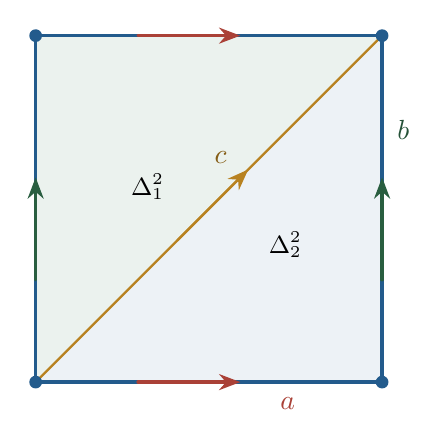
\begin{tikzpicture}[>=Stealth,line cap=round,line join=round,
 x=1cm,y=1cm]
 \coordinate (a) at (0,0);
 \coordinate (b) at (4.4,0);
 \coordinate (c) at (4.4,4.4);
 \coordinate (d) at (0,4.4);
 \fill[manifoldblue!8] (a)--(b)--(c)--cycle;
 \fill[manifoldgreen!10] (a)--(d)--(c)--cycle;
 \draw[manifoldblue,very thick] (a)--(b)--(c)--(d)--cycle;
 \draw[manifoldgold!90!black,thick] (a)--(c);
 \draw[manifoldgold!90!black,thick,-{Stealth[length=2.7mm]}]
  (1.8,1.8)--(2.7,2.7);
 \draw[manifoldred,very thick,-{Stealth[length=2.7mm]}]
  (1.3,0)--(2.6,0);
 \draw[manifoldred,very thick,-{Stealth[length=2.7mm]}]
  (1.3,4.4)--(2.6,4.4);
 \draw[manifoldgreen!75!black,very thick,-{Stealth[length=2.7mm]}]
  (0,1.3)--(0,2.6);
 \draw[manifoldgreen!75!black,very thick,-{Stealth[length=2.7mm]}]
  (4.4,1.3)--(4.4,2.6);
 \node[manifoldred,below=2pt] at (3.2,0) {$a$};
 \node[manifoldgreen!65!black,right=2pt] at (4.4,3.2) {$b$};
 \node[manifoldgold!65!black,above left=2pt]
  at (2.6,2.6) {$c$};
 \foreach \p in {a,b,c,d}
  \fill[manifoldblue] (\p) circle(2.3pt);
 \node[font=\small] at (1.42,2.48) {$\Delta^2_1$};
 \node[font=\small] at (3.17,1.74) {$\Delta^2_2$};
\end{tikzpicture}
\caption{Torus z dwóch sympleksów: boki o tych samych
kolorach i kierunkach sklejamy ze sobą. Przekątna
pozostaje trzecią krawędzią. Wszystkie cztery narożniki
reprezentują ten sam wierzchołek torusa.}
\label{fig:delta-torus}
\end{figure}

\section{CW-kompleksy i dołączanie komórek}
\label{sec:cw-kompleksy}

Trójkąty są wygodne do obliczeń, lecz
potrafią wymagać wielu wierzchołków.
Komórka pozwala dołączyć naraz cały
otwarty dysk, przy czym jego brzeg
może biec po starszej części przestrzeni
w sposób nietrywialny.

\begin{definicja}[Dołączenie komórki]
\index{dolaczenie komorki@Dołączenie komórki}
\label{def:dolaczenie-komorki}
Niech $Y$ będzie przestrzenią i
$\varphi:S^{n-1}=\partial D^n\to Y$
odwzorowaniem ciągłym, $n\geq1$.
\emph{Dołączeniem $n$-komórki} jest
przestrzeń ilorazowa
\[
 Y\cup_\varphi D^n
 :=(Y\sqcup D^n)/(z\sim\varphi(z)
 \text{ dla }z\in S^{n-1}).
\]
Obraz wnętrza dysku oznaczamy $e^n$.
Odwzorowanie z dysku do ilorazu jest
\emph{odwzorowaniem charakterystycznym}
tej komórki; $\varphi$ nazywamy
\emph{odwzorowaniem dołączającym}.
W wymiarze $0$ po prostu dołączamy
izolowany punkt, gdyż
$S^{-1}=\varnothing$.
\end{definicja}

Naturalne włączenie $Y$ w przestrzeń dołączoną jest osadzeniem
na zbiór domknięty. Dla każdego domkniętego $F\subseteq Y$
przeciwobraz jego obrazu w $Y\sqcup D^n$ jest równy
$F\sqcup\varphi^{-1}(F)$ i jest domknięty; dotyczy to również $F=Y$.
Ponieważ na punktach $Y$ nie wprowadzamy nowych utożsamień,
dostajemy zamknięte osadzenie. Wnętrze $D^n$ jest natomiast
otwartym zbiorem nasyconym, bez żadnych utożsamień, więc przechodzi
homeomorficznie na otwartą komórkę $e^n$.

Topologia ilorazowa z
Definicji~\ref{def:topologia-ilorazowa}
ma tu konkretne znaczenie. Jeśli
$F:Y\cup_\varphi D^n\to Z$
ma być ciągła, wystarczy podać
ciągłe $F_Y:Y\to Z$ i
$F_D:D^n\to Z$ zgodne na brzegu:
$F_D(z)=F_Y(\varphi(z))$.
Istotnie, takie odwzorowania dają ciągłe
odwzorowanie na rozłącznej sumie, stałe
na każdej klasie sklejenia;
uniwersalna własność ilorazu
przenosi je na iloraz.
To jest praktyczny sposób
konstruowania odwzorowań na przestrzeniach
sklejonych.

\begin{definicja}[CW-kompleks]
\index{cw-kompleks@CW-kompleks}
\label{def:cw-kompleks}
\emph{CW-kompleks} $X$ jest przestrzenią Hausdorffa budowaną
ze szkieletów $X^0\subseteq X^1
\subseteq X^2\subseteq\cdots$:
$X^0$ jest dyskretnym zbiorem punktów,
a $X^n$ powstaje z $X^{n-1}$
przez dołączenie rodziny $n$-dysków
odwzorowaniami $S^{n-1}\to X^{n-1}$.
Przestrzeń $X=\bigcup_n X^n$
ma \emph{topologię słabą}:
$A\subseteq X$ jest domknięty,
dokładnie wtedy, gdy przeciwobraz $A$ pod każdym
odwzorowaniem charakterystycznym $D^n\to X$
jest domknięty. Wymagamy ponadto
\emph{skończoności domknięć komórek}:
domknięcie każdej komórki
spotyka tylko skończenie wiele
komórek. Litery CW przypominają
te dwa warunki
(\emph{closure-finite}, \emph{weak topology}).
\emph{Podkompleks CW} to suma komórek
domknięta w $X$; jeśli zawiera komórkę,
zawiera także całe jej domknięcie.
\end{definicja}

\begin{figure}[!htbp]
\centering
\begin{tikzpicture}[>=Stealth,line cap=round,line join=round]
 \node[font=\bfseries] at (0,3.02) {$X^0$};
 \node[font=\bfseries] at (4.33,3.02) {$X^1$};
 \node[font=\bfseries] at (8.68,3.02) {$X^2$};
 % 0-komórka.
 \fill[manifoldred] (0,1.39) circle(3.7pt);
 \node[below=7pt] at (0,1.39) {$e^0=\{v\}$};
 % Dołączenie 1-komórki: oba końce trafiają do v.
 \draw[manifoldblue,line width=2.5pt]
  (4.33,1.45) circle(1.03);
 \fill[manifoldred] (4.33,.42) circle(3.7pt);
 \node[manifoldblue!85!black] at (4.33,1.45) {$e^1$};
 \draw[->,manifoldblue!75!black,thin]
  (4.62,1.74)--({4.33+1.03*cos(45)},{1.45+1.03*sin(45)});
 \node[below=7pt] at (4.33,.42) {$v$};
 \draw[->,manifoldgold!80!black,thick]
  (1.22,1.54)--(3.08,1.54)
  node[midway,above=5pt,font=\small] {dołącz $e^1$};
 % Dołączenie 2-komórki: brzeg dysku biegnie po okręgu.
 \fill[manifoldgreen!18] (8.68,1.45) circle(1.03);
 \draw[manifoldblue,line width=2.5pt]
  (8.68,1.45) circle(1.03);
 \fill[manifoldred] (8.68,.42) circle(3.7pt);
 \node[manifoldgreen!65!black] at (8.68,1.45) {$e^2$};
 \node[below=7pt] at (8.68,.42) {$v$};
 \draw[->,manifoldgold!80!black,thick]
  (5.58,1.54)--(7.35,1.54)
  node[midway,above=5pt,font=\small] {dołącz $e^2$};
\end{tikzpicture}
\caption{Przykłady kolejnych wymiarów CW: punkt
$X^0=\{v\}$, okrąg $X^1\cong S^1$ otrzymany
przez sklejenie obu końców $1$-komórki z $v$,
oraz dysk $X^2\cong D^2$ po dołączeniu
$2$-komórki wzdłuż całego okręgu.
Czerwony punkt, niebieski łuk i zielone wnętrze
oznaczają odpowiednio otwarte komórki
wymiarów $0,1,2$.}
\label{fig:cw-wymiary}
\end{figure}

W kompleksie skończonym warunki
topologiczne łatwo sprawdzić
bez osobnej teorii granic:
topologia słaba jest ilorazową
topologią sklejania skończenie
wielu dysków, a domknięcie
każdej komórki spotyka
tylko skończenie wiele innych.
Przy nieskończenie wielu komórkach
topologia słaba jest konieczna,
aby ciągłość dało się sprawdzać
na wszystkich domkniętych komórkach.

\begin{stwierdzenie}[Sympleksy dają komórki]
\label{prop:sympleksy-cw}
Skończony kompleks symplicjalny i
skończony $\Delta$-kompleks są
CW-kompleksami: ich otwarte komórki
to obrazy wnętrz sympleksów.
\end{stwierdzenie}
\begin{proof}
Indukujemy po wymiarze. Szkielet
zerowy składa się z wierzchołków.
Wnętrze każdego $n$-sympleksu
jest rozłączne z obrazami innych
wnętrz, a brzeg jest sumą ścian
zawartych w poprzednim szkielecie.
Stwierdzenie~\ref{prop:brzeg-sympleksu}
pozwala traktować sympleks
jako dysk $D^n$, którego
odwzorowanie na brzegu jest odwzorowaniem dołączającym.
Warunek o topologii jest w
Definicji~\ref{def:delta-kompleks}
podany wprost, a dla skończonej
realizacji symplicjalnej wynika
z topologii skończonej sumy zwartych sympleksów:
ciągła surjekcja z tej sumy na $|K|\subseteq\R^V$ jest domknięta,
gdyż obrazy zbiorów domkniętych są zwarte w przestrzeni Hausdorffa.
Jest więc odwzorowaniem ilorazowym, co daje właśnie wymaganą topologię.
Skończona liczba sympleksów
zapewnia skończoność domknięć komórek.
\end{proof}

\begin{przyklad}[Minimalne struktury komórkowe]
\label{prz:cw-sfera-torus}
\begin{enumerate}[label=(\arabic*),leftmargin=*]
\item Dla $n\geq1$ sfera $S^n$
      ma jedną $0$-komórkę i jedną
      $n$-komórkę:
      $D^n/S^{n-1}\cong S^n$.
      Jawny homeomorfizm opisujemy
      poniżej.
      Dla $S^0$ używamy dwóch
      $0$-komórek.
\item Torus ma jedną $0$-komórkę,
      dwie $1$-komórki $a,b$ oraz
      jedną $2$-komórkę. Obchodząc
      brzeg kwadratu z
      Rysunku~\ref{fig:delta-torus},
      otrzymujemy słowo
      $aba^{-1}b^{-1}$ w
      $S^1\vee S^1$.
      Dwa trójkąty realizacji
      $\Delta$-kompleksowej zostały
      zastąpione jednym dyskiem,
      którego odwzorowanie dołączające
      zapamiętuje sklejanie.
\end{enumerate}
\end{przyklad}

\begin{przyklad}[Sfera $S^2$ bez $1$-komórek]
\label{prz:cw-s2}
Weźmy $X^0=\{v\}$ i nie dołączajmy
żadnej $1$-komórki, więc $X^1=X^0$.
Niech odwzorowanie dołączające
$\varphi:\partial D^2=S^1\to\{v\}$
będzie stałe. Wtedy
\[
 X^2=X^1\cup_\varphi D^2
 \cong D^2/\partial D^2\cong S^2.
\]
Cały brzeg dysku staje się \emph{jednym}
punktem $v$; obraz jego wnętrza
jest jedną otwartą $2$-komórką
$e^2=S^2\setminus\{v\}\cong\R^2$.
Rysunek~\ref{fig:cw-s2} pokazuje to
sklejenie. W szczególności
$X^1$ nie jest okręgiem:
okrąg po lewej stronie rysunku
to brzeg \emph{dołączanego dysku},
a nie komórka przestrzeni wynikowej.
\end{przyklad}

\begin{figure}[!htbp]
\centering
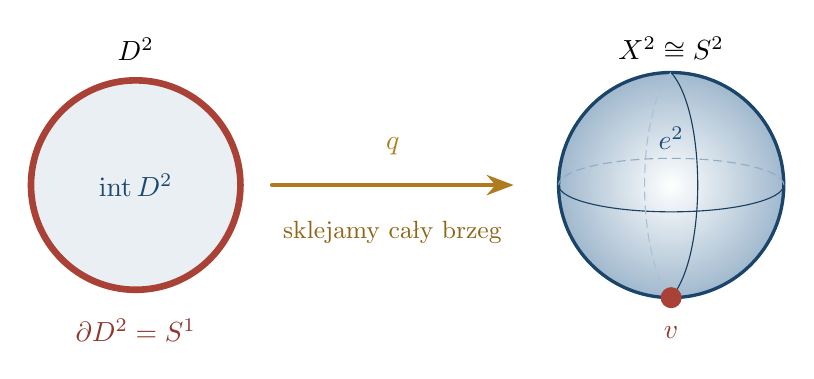
\begin{tikzpicture}[>=Stealth,line cap=round,line join=round]
 % Dysk przed sklejeniem: czerwony brzeg zapada się do v.
 \fill[manifoldblue!10] (0,1.85) circle(1.33);
 \draw[manifoldred,line width=2.4pt] (0,1.85) circle(1.33);
 \node[font=\bfseries] at (0,3.58) {$D^2$};
 \node[manifoldblue!80!black] at (0,1.85) {$\operatorname{int}D^2$};
 \node[manifoldred!85!black,below=7pt]
  at (0,.52) {$\partial D^2=S^1$};
 % Sklejenie brzegu do jednego punktu.
 \draw[->,manifoldgold!85!black,line width=1.5pt]
  (1.73,1.85)--(4.8,1.85)
  node[midway,above=7pt] {$q$};
 \node[font=\small,manifoldgold!70!black]
  at (3.26,1.25) {sklejamy cały brzeg};
 % Sfera w stylistyce rysunku 1.4: jasny środek, tył i przód łuków.
 \shade[inner color=white,outer color=manifoldblue!43]
  (6.8,1.85) circle(1.43);
 \draw[manifoldblue!75!black,very thick]
  (6.8,1.85) circle(1.43);
 \draw[manifoldblue!50,densely dashed,thin]
  (8.23,1.85) arc[start angle=0,end angle=180,x radius=1.43,y radius=.34];
 \draw[manifoldblue!70!black,thin]
  (5.37,1.85) arc[start angle=180,end angle=360,x radius=1.43,y radius=.34];
 \draw[manifoldblue!38,densely dashed,thin]
  (6.8,3.28) .. controls (6.35,2.76) and (6.35,.94) .. (6.8,.42);
 \draw[manifoldblue!65!black,thin]
  (6.8,3.28) .. controls (7.25,2.76) and (7.25,.94) .. (6.8,.42);
 \fill[manifoldred] (6.8,.42) circle(3.8pt);
 \node[font=\bfseries] at (6.8,3.58) {$X^2\cong S^2$};
 \node[manifoldblue!85!black] at (6.8,2.44) {$e^2$};
 \node[manifoldred!85!black,below=7pt] at (6.8,.42) {$v$};
\end{tikzpicture}
\caption{Struktura CW sfery: $D^2$ dołączamy do
punktu $v$ odwzorowaniem stałym na całym brzegu;
$q:D^2\to D^2/\partial D^2$ jest mapą ilorazową.
W powstałej sferze czerwony punkt to
jedyne $e^0$, a cała pozostała powierzchnia
to jedna otwarta komórka $e^2$.
Nie występują komórki wymiaru $1$.}
\label{fig:cw-s2}
\end{figure}

\begin{uwaga}[Uwaga o ilorazie dysku]
W punkcie (1) nie potrzebujemy
identyfikować półkuli z ilorazem
za pomocą niejawnego rysunku.
Istnieje jawne ciągłe odwzorowanie
$D^n\to S^n\subseteq\R^{n+1}$,
\[
 x\longmapsto
 \bigl(\sin(\pi\|x\|)\,x/\|x\|,
       \cos(\pi\|x\|)\bigr)
 \quad(x\ne0),
\]
z wartością $(0,\ldots,0,1)$
w $x=0$. Cały brzeg $\|x\|=1$
przechodzi w biegun południowy,
a na wnętrzu odwzorowanie jest iniektywne
i pokrywa sferę bez tego bieguna.
Przechodzi więc na ciągłą bijekcję
$D^n/S^{n-1}\to S^n$, która jest
homeomorfizmem przez zwartość
dziedziny i własność Hausdorffa
sfery.
\end{uwaga}

\begin{twierdzenie}[Co robi dołączenie komórki z $\pi_1$?]
\label{thm:pi1-dolaczenie-komorki}
Niech $Y$ będzie łukowo spójna,
a $X=Y\cup_\varphi D^n$.
Jeśli $n=2$, po wyborze drogi od
punktu bazowego do $\varphi(S^1)$
grupa $\pi_1(X)$ jest ilorazem
$\pi_1(Y)$ przez domknięcie normalne
klasy pętli $\varphi$.
Jeśli $n\geq3$, włączenie
$Y\hookrightarrow X$ wyznacza
izomorfizm na $\pi_1$.
\end{twierdzenie}
\begin{proof}
W dysku wybierzmy promień $r=\|x\|$.
Otwarty w $X$ zbiór $U$ złożony
z $Y$ i pasa $r>1/3$ deformuje
się na $Y$: przesuwamy punkty
pasa promieniowo do $r=1$,
a punkty $Y$ zostawiamy. Na części dyskowej homotopia ma wzór
$ru\mapsto((1-t)r+t)u$, gdzie $u\in S^{n-1}$.
Wyjaśnijmy ciągłość przy sklejanym $Y$. Dla otwartego otoczenia
$O$ punktu $y\in Y$ zmniejszamy jego część dyskową do punktów $ru$,
dla których $\varphi(u)\in O\cap Y$ i cały odcinek
$\{\rho u:r\leq\rho\leq1\}$ leży w przeciwobrazie $O$.
Ta część jest otwarta: zawieranie zwartego odcinka w zbiorze
otwartym zachowuje się przy małej zmianie $r,u$.
Wraz z $O\cap Y$ tworzy otwarte otoczenie $y$ w ilorazie,
którego obraz przez homotopię pozostaje w $O$ dla wszystkich $t$.
Dowodzi to ciągłości przy $Y$; na wnętrzu dysku wynika ona z podanego wzoru.
Drugi otwarty zbiór $V$ jest
obrazem $r<2/3$; jest to
ściągalne wnętrze dysku.
Przecięcie $U\cap V$ to pierścień
$1/3<r<2/3$, homotopijnie
równoważny $S^{n-1}$.
Jest łukowo spójne dla $n\geq2$.
Otwartość obu zbiorów sprawdzamy przed sklejeniem:
przeciwobrazy $U$ to całe $Y$ i otwarty w $D^n$ pas $r>1/3$,
a przeciwobraz $V$ to $r<2/3$, bez punktów $Y$.

Twierdzenie~\ref{thm:van-kampen}
z $G_V=1$ mówi, że $\pi_1(X)$
jest ilorazem $\pi_1(U)\cong\pi_1(Y)$
przez domknięcie normalne obrazu
$\pi_1(U\cap V)$. Przy $n=2$
generator $\pi_1(S^1)\cong\Z$
po przejściu przez retrakcję
$U\to Y$ staje się pętlą
$\varphi$ (z uwzględnieniem
drogi do punktu bazowego).
Przy $n\geq3$ mamy
$\pi_1(S^{n-1})=0$ z
Przykładu~\ref{prz:pi1-sfera},
więc nie pojawia się żadna
relacja ani nowy generator.
\end{proof}

\begin{przyklad}[Torus i powierzchnia rzutowa]
\label{prz:pi1-torus-rp2}
Dla torusa część jednowymiarowa
jest $S^1\vee S^1$, z grupą
$F(a,b)$ z Przykładu~\ref{prz:pi1-dwa-okregi}.
Dołączona $2$-komórka wymusza
$aba^{-1}b^{-1}=1$, czyli
\[
 \pi_1(T^2)\cong
 \langle a,b\mid ab=ba\rangle
 \cong\Z^2.
\]
Drugim przykładem jest
$\R P^2$: dysk będący górną
półkulą $S^2$ ma na brzegu
antypody utożsamione, więc
$\R P^2$ ma $0$-komórkę,
      $1$-komórkę i $2$-komórkę
      dołączoną do $S^1\cong\R P^1$
      odwzorowaniem odpowiadającym
      $z\mapsto z^2$ (liczba owinięć wynosi $2$).
      Istotnie, $S^1/(z\sim-z)\to S^1$, $[z]\mapsto z^2$,
      jest homeomorfizmem jako ciągła bijekcja ze zwartej
      przestrzeni do przestrzeni Hausdorffa; odwzorowanie dołączające
      przechodzi przez ten iloraz. Pełny obieg brzegu daje zatem dwa obiegi
      $1$-szkieletu, co wyjaśnia relację $a^2=1$.
      Zatem
\[
 \pi_1(\R P^2)
 \cong\langle a\mid a^2=1\rangle
 \cong\Z/2\Z.
\]
W obu przykładach relacja grupowa pochodzi bezpośrednio
z przebiegu brzegu dołączanej $2$-komórki.
\end{przyklad}

\begin{uwaga}[Granica obecnego rozdziału]
Sympleksy i komórki dają
konkretne przestrzenie, a ich
odwzorowania dołączające kodują sposób
sklejenia. W następnym rozdziale
zorientowanym sympleksom przypiszemy
generatory łańcuchów, a ich ścianom
operator brzegu $\partial$.
Sprawdzimy $\partial^2=0$,
porównamy homologię symplicjalną,
singularną i komórkową oraz
wykorzystamy długie ciągi
z Rozdziału~\ref{ch:algebra-homologiczna}.
Wyższe grupy homotopii i twierdzenie
Hurewicza wymagają już tak
zbudowanej homologii przestrzeni.
\end{uwaga}

\section*{Dalsza lektura}
\addcontentsline{toc}{section}{Dalsza lektura}
Pełne rozwinięcie teorii homotopii,
nakryć, kompleksów CW i
$\Delta$-kompleksów podaje
Allen Hatcher, \emph{Algebraic Topology},
rozdziały 0 i 1 oraz początek rozdziału 2,
\url{https://pi.math.cornell.edu/~hatcher/AT/AT.pdf}.
W tym rozdziale wyprowadziliśmy
podstawowe własności, które
wykorzystamy do budowania homologii.

\clearpage

\chapter{Homologia przestrzeni}
\label{ch:homologia-przestrzeni}

W Rozdziale~\ref{ch:algebra-homologiczna} homologia była
niezmiennikiem \emph{kompleksu łańcuchowego}.
Teraz przypiszemy taki kompleks przestrzeni. Najpierw
użyjemy sympleksów z Rozdziału~\ref{ch:topologia-algebraiczna-podstawy};
potem zastąpimy je wszystkimi ciągłymi obrazami sympleksów,
aby móc badać przestrzenie bez wybranej triangulacji. Na końcu
zobaczymy, dlaczego do obliczeń zwykle wystarczy
kilka komórek CW.

Intuicja jest jedna: cykl to suma zorientowanych kawałków
bez brzegu, a brzeg to cykl, który ogranicza kawałek
o wymiar wyższy. Iloraz
\[
 H_n(X;\Z)=
 \frac{\{\text{$n$-cykle w $X$}\}}
 {\{\text{brzegi $(n+1)$-łańcuchów w $X$}\}}
\]
odróżnia na przykład pętlę będącą brzegiem na tarczy od pętli
obiegającej dziurę. Pracujemy nad $\Z$; zmianę
współczynników omawia
Twierdzenie~\ref{thm:homologia-char-zero},
a konkretny rachunek znajduje się poniżej.

\section{Łańcuchy symplicjalne: orientacja i brzeg}
\label{sec:homologia-symplicjalna}

\begin{definicja}[Kompleks łańcuchów symplicjalnych]
\index{kompleks lancuchow symplicjalnych@Kompleks łańcuchów symplicjalnych}
\label{def:homologia-symplicjalna}
Niech $K$ będzie skończonym kompleksem symplicjalnym
z Definicji~\ref{def:kompleks-symplicjalny}.
Ustalmy porządek jego wierzchołków. Grupa
$C_n^\Delta(K)$ jest wolną grupą abelową z bazą
wszystkich $n$-sympleksów zapisanych w porządku
$[v_0,\ldots,v_n]$. Jeśli wierzchołki wypiszemy
w innej kolejności, przyjmujemy zasadę
\[
 [v_{\pi(0)},\ldots,v_{\pi(n)}]
 =\operatorname{sgn}(\pi)[v_0,\ldots,v_n].
\]
Zatem odwrócenie orientacji zmienia znak, a dwa
różne sympleksy nadal dają niezależne generatory.
Dla $n\geq1$ określamy
\begin{equation}\label{eq:brzeg-symplicjalny}
 \partial_n[v_0,\ldots,v_n]
 =\sum_{i=0}^n(-1)^i
 [v_0,\ldots,\widehat v_i,\ldots,v_n],
 \qquad \partial_0=0.
\end{equation}
Rozszerzamy $\partial$ liniowo na sumy
o całkowitych współczynnikach. Dla $n<0$ przyjmujemy $C_n^\Delta(K)=0$.
\end{definicja}

Znak ściany nie jest ozdobą: kierunek odziedziczony
przez brzeg wypełnionego trójkąta musi być spójny.
Dla $e=[v_0,v_1]$ i $t=[v_0,v_1,v_2]$ dostajemy
\[
 \partial e=[v_1]-[v_0],\qquad
 \partial t=[v_1,v_2]-[v_0,v_2]+[v_0,v_1].
\]
Drugą równość można zapisać
$\partial t=[v_0,v_1]+[v_1,v_2]+[v_2,v_0]$.
Jest to obieg brzegu trójkąta.

\begin{figure}[!htbp]
\centering
\begin{tikzpicture}[>=Stealth,line cap=round,line join=round]
 \coordinate (a) at (0,0); \coordinate (b) at (3.3,0);
 \coordinate (c) at (1.35,2.55);
 \fill[manifoldblue!13] (a)--(b)--(c)--cycle;
 \draw[manifoldblue!65!black,line width=1.6pt]
  (a)--(b)--(c)--cycle;
 \draw[->,manifoldred,line width=1.5pt]
  (.7,-.13)--(2.5,-.13);
 \draw[->,manifoldred,line width=1.5pt]
  (3.1,.38)--(1.8,2.07);
 \draw[->,manifoldred,line width=1.5pt]
  (1.04,2.1)--(.13,.39);
 \foreach \p in {a,b,c}{\fill[manifoldgold!85!black] (\p) circle(2.8pt);}
 \node[below left] at (a) {$v_0$};
 \node[below right] at (b) {$v_1$};
 \node[above] at (c) {$v_2$};
 \node[manifoldblue!75!black] at (1.4,.84) {$t$};
 \node[align=left,anchor=west,text width=5.5cm] at (4.1,1.38)
  {$\partial t=e_{01}+e_{12}+e_{20}$\\[3pt]
   zewnętrzna pętla jest brzegiem, gdy wnętrze $t$
   należy do przestrzeni};
\end{tikzpicture}
\caption{Zorientowany brzeg trójkąta. Usunięcie jego
wnętrza pozostawia cykl, który w samym okręgu
nie jest już brzegiem żadnego $2$-łańcucha.}
\label{fig:homologia-trojkat}
\end{figure}

\begin{twierdzenie}[Brzeg brzegu znika]
\label{thm:brzeg-brzegu}
Odwzorowania~\eqref{eq:brzeg-symplicjalny}
spełniają $\partial_{n-1}\partial_n=0$.
Wobec tego
\[
 H_n^\Delta(K):=
 \ker(\partial_n:C_n^\Delta(K)\to C_{n-1}^\Delta(K))
 \big/
 \operatorname{im}(\partial_{n+1})
\]
jest dobrze określoną grupą. Licznik składa
się z \emph{cykli}, mianownik z \emph{brzegów}.
\end{twierdzenie}
\begin{proof}
Dla $n=1$ wynika to z $\partial_0=0$.
Niech $n\geq2$ i weźmy generator
$[v_0,\ldots,v_n]$. Każda jego ściana
o wymiarze $n-2$ powstaje po usunięciu
pewnych dwóch wierzchołków $v_i,v_j$,
$i<j$, dokładnie na dwa sposoby.
Usunięcie najpierw $v_i$, a następnie
$v_j$ (ma on już pozycję $j-1$) daje
współczynnik $(-1)^i(-1)^{j-1}$.
W przeciwnej kolejności współczynnik
wynosi $(-1)^j(-1)^i$.
Ich suma to
$(-1)^{i+j-1}+(-1)^{i+j}=0$.
Dotyczy to każdej ściany z osobna,
więc $\partial^2$ znika na bazie,
a przez liniowość na całej grupie.
Stąd $\operatorname{im}\partial_{n+1}
\subseteq\ker\partial_n$, co pozwala
utworzyć podany iloraz.
\end{proof}

\begin{przyklad}[Odcinek, okrąg, tarcza]
\label{prz:homologia-odcinek-okrag}
Odcinek ma dwa wierzchołki $v_0,v_1$
i jedną krawędź $e$. Odwzorowanie
$\partial_1:\Z e\to\Z v_0\oplus\Z v_1$
przypisuje $me\mapsto m(v_1-v_0)$.
Ma zerowe jądro, więc $H_1^\Delta=0$,
a w ilorazie $H_0^\Delta$ obie klasy
wierzchołków są równe. Otrzymujemy $\Z$.

Teraz weźmy obwód trójkąta, bez wnętrza,
i ustawmy kierunki $e_{01},e_{12},e_{20}$.
Każdy $1$-łańcuch
$ae_{01}+be_{12}+ce_{20}$ jest cyklem
dokładnie wtedy, gdy $a=b=c$
(współczynnik przy każdym wierzchołku
w jej brzegu musi być zerem).
Nie ma tu $2$-sympleksów, a więc
$H_1^\Delta\cong\Z$ z generatorem
$e_{01}+e_{12}+e_{20}$.
Jeśli wstawimy wnętrze $t$, ten sam
cykl staje się $\partial t$ i
$H_1^\Delta$ znika. Rysunek~\ref{fig:homologia-trojkat}
pokazuje dokładnie tę zmianę.
\end{przyklad}

W $\Delta$-kompleksie z
Definicji~\ref{def:delta-kompleks} postępujemy
podobnie: każdy \emph{sympleks charakterystyczny}
jest osobnym generatorem, nawet jeżeli jego
różne ściany mają ten sam obraz. Brzeg
jest sumą obrazów ścian z ich znakami;
po identyfikacji mogą się one wzajemnie
skasować. Tak właśnie sklejony odcinek
z jednym wierzchołkiem ma $\partial e=v-v=0$.

\begin{stwierdzenie}[Składowe i $H_0$]
\label{prop:h0-symplicjalne}
Jeżeli $K$ ma $c$ składowych łukowych,
to $H_0^\Delta(K)\cong\Z^c$.
\end{stwierdzenie}
\begin{proof}
Ponieważ $\partial_0=0$, grupa $H_0$
to wolna grupa na wierzchołkach
modulo relacje
$v_j-v_i=\partial[v_i,v_j]$
dla krawędzi. Idąc po drodze krawędziowej,
utożsamiamy klasy wszystkich wierzchołków
jej składowej. Dwa wierzchołki tej samej
składowej $|K|$ można połączyć taką drogą:
wszystkie wierzchołki jednego sympleksu należą do tej samej
składowej grafu krawędzi. Sympleksy przypisane jednej takiej
składowej tworzą podkompleks. Jego realizacja i jej dopełnienie
są domknięte jako skończone sumy domkniętych sympleksów,
więc są też otwarte. Droga nie może przejść między tymi zbiorami.
Każdy punkt sympleksu można natomiast połączyć odcinkiem z wierzchołkiem.
Składowe grafu odpowiadają zatem dokładnie składowym łukowym $|K|$. Wreszcie żadna
relacja nie łączy różnych składowych,
bo obie końcówki każdej krawędzi leżą
w jednej. W każdej składowej pozostaje
więc jeden wolny generator.
\end{proof}

\section{Łańcuchy singularne i niezmienniczość homotopijna}
\label{sec:homologia-singularna}

Triangulacja bywa trudna do znalezienia. W konstrukcji
singularnej sam wybór \emph{ciągłego} odwzorowania
standardowego sympleksu do przestrzeni tworzy
generator; nie żądamy różnowartościowości ani
ładnego kształtu jego obrazu.

\begin{definicja}[Homologia singularna]
\index{homologia singularna@Homologia singularna}
\label{def:homologia-singularna}
\emph{Singularny $n$-sympleks} w $X$ to dowolne
ciągłe odwzorowanie $\sigma:\Delta^n\to X$.
Niech $C_n(X)$ będzie wolną grupą abelową
na wszystkich takich odwzorowaniach; dla $n<0$ przyjmujemy $C_n(X)=0$.
W szczególności
dwa różne odwzorowania o tym samym obrazie są
różnymi generatorami. Niech
$\iota_i:\Delta^{n-1}\to\Delta^n$
będzie afinicznym włączeniem ściany
naprzeciw $i$-tego wierzchołka. Kładziemy
\begin{equation}\label{eq:singular-boundary}
 \partial\sigma=\sum_{i=0}^n(-1)^i
 \sigma\circ\iota_i\quad(n\geq1),
 \qquad \partial:C_0(X)\to0,
 \qquad H_n(X):=H_n(C_\bullet(X),\partial).
\end{equation}
\end{definicja}

Obliczenie $\partial^2=0$ jest słowo w słowo
rachunkiem dwóch usuwanych wierzchołków
z dowodu Twierdzenia~\ref{thm:brzeg-brzegu}.
Teraz pojawia się nawet singularny sympleks
stały: nie odrzucamy go na poziomie
łańcuchów, gdyż później jego wkład może
być brzegiem.

\begin{figure}[!htbp]
\centering
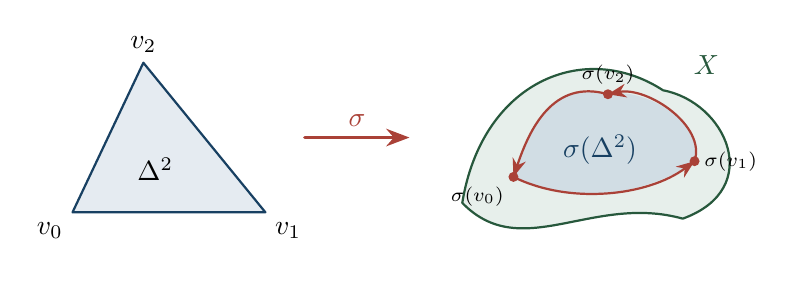
\begin{tikzpicture}[>=Stealth,line cap=round,line join=round]
 \coordinate (a) at (0,0); \coordinate (b) at (2.45,0);
 \coordinate (c) at (.9,1.9);
 \fill[manifoldblue!12] (a)--(b)--(c)--cycle;
 \draw[manifoldblue!70!black,thick] (a)--(b)--(c)--cycle;
 \node[below left] at (a) {$v_0$};
 \node[below right] at (b) {$v_1$};
 \node[above] at (c) {$v_2$};
 \node at (1.05,.55) {$\Delta^2$};
 \draw[->,manifoldred,very thick] (2.95,.95)--(4.28,.95)
  node[midway,above] {$\sigma$};
 \fill[manifoldgreen!12]
  (4.95,.12) .. controls (5.7,-.65) and (6.6,.24) ..
  (7.75,-.08) .. controls (8.8,.3) and (8.3,1.4) ..
  (7.5,1.55) .. controls (6.5,2.2) and (5.2,1.66) ..
  (4.95,.12);
 \draw[manifoldgreen!70!black,thick]
  (4.95,.12) .. controls (5.7,-.65) and (6.6,.24) ..
  (7.75,-.08) .. controls (8.8,.3) and (8.3,1.4) ..
  (7.5,1.55) .. controls (6.5,2.2) and (5.2,1.66) ..
  (4.95,.12);
 \fill[manifoldblue!25,opacity=.7]
  (5.6,.45) .. controls (6.3,.1) and (7.3,.2) .. (7.9,.65)
  .. controls (8.05,1.1) and (7.3,1.6) .. (6.8,1.5)
  .. controls (6.1,1.7) and (5.8,1.05) .. (5.6,.45);
 \draw[manifoldred,thick,->]
  (5.6,.45) .. controls (6.3,.1) and (7.3,.2) .. (7.9,.65);
 \draw[manifoldred,thick,->]
  (7.9,.65) .. controls (8.05,1.1) and (7.3,1.6) .. (6.8,1.5);
 \draw[manifoldred,thick,->]
  (6.8,1.5) .. controls (6.1,1.7) and (5.8,1.05) .. (5.6,.45);
 \foreach \x/\y in {5.6/.45,7.9/.65,6.8/1.5}
  {\fill[manifoldred] (\x,\y) circle(1.8pt);}
 \node[font=\scriptsize,below left] at (5.6,.45) {$\sigma(v_0)$};
 \node[font=\scriptsize,right] at (7.9,.65) {$\sigma(v_1)$};
 \node[font=\scriptsize,above] at (6.8,1.5) {$\sigma(v_2)$};
 \node[manifoldgreen!70!black] at (8.05,1.87) {$X$};
 \node[manifoldblue!70!black] at (6.7,.8) {$\sigma(\Delta^2)$};
\end{tikzpicture}
\caption{Singularny sympleks jest odwzorowaniem do $X$, niekoniecznie
płaskim trójkątem. Jego brzeg liczymy
z ograniczeń odwzorowania $\sigma$ do trzech ścian.}
\label{fig:singular-simplex}
\end{figure}

\begin{stwierdzenie}[Ciągłe odwzorowania działają na homologii]
\label{prop:funktor-singularny}
Jeśli $f:X\to Y$ jest ciągłe, to
$f_\#:C_n(X)\to C_n(Y)$,
$f_\#(\sigma)=f\circ\sigma$,
jest odwzorowaniem łańcuchowym. Wyznacza homomorfizm
$f_*:H_n(X)\to H_n(Y)$, przy czym
$(g\circ f)_*=g_*\circ f_*$ oraz
$(\id_X)_*=\id_{H_n(X)}$.
\end{stwierdzenie}
\begin{proof}
Na pojedynczym generatorze
\[
 \partial(f\circ\sigma)
 =\sum_i(-1)^i f\circ\sigma\circ\iota_i
 =f_\#(\partial\sigma).
\]
Równość na sumach wynika z liniowości.
Zatem obraz cyklu jest cyklem, a obraz
brzegu brzegiem, więc $f_*$ jest
dobrze określony na ilorazie.
Równości dotyczące składania sprawdzamy
już na $\sigma$:
$g_\#f_\#(\sigma)=g\circ f\circ\sigma$.
\end{proof}

\begin{przyklad}[Punkt]
\label{prz:homologia-punktu}
Dla $X=\{*\}$ w każdym stopniu jest
dokładnie jeden singularny sympleks
stały $c_n$, więc $C_n(X)\cong\Z$.
Jego brzeg to
$\partial c_n=(\sum_{i=0}^n(-1)^i)c_{n-1}$:
dla $n$ nieparzystego współczynnik
jest $0$, dla dodatniego parzystego $1$.
Kompleks ma więc postać
\[
 \cdots\xrightarrow{\;0\;}\Z
 \xrightarrow{\;1\;}\Z
 \xrightarrow{\;0\;}\Z
 \xrightarrow{\;1\;}\Z
 \xrightarrow{\;0\;}\Z\longrightarrow0,
\]
gdzie prawy skraj to $C_0$; precyzyjnie
$\partial_1=0$, $\partial_2=1$.
Stąd $H_0(*)=\Z$ i $H_n(*)=0$ dla $n>0$.
\end{przyklad}

\begin{stwierdzenie}[Składowe łukowe]
\label{prop:h0-singularne}
Grupa $H_0(X)$ jest wolna na składowych
łukowych $X$. W szczególności
dla przestrzeni niepustej łukowo spójnej
$H_0(X)\cong\Z$.
\end{stwierdzenie}
\begin{proof}
Każdy punkt $x$ jest singularnym
$0$-sympleksem, więc $C_0(X)$
jest wolną grupą na punktach.
Dla drogi $\gamma:[0,1]=\Delta^1\to X$
mamy $\partial\gamma=[\gamma(1)]-
[\gamma(0)]$. Punkty w jednej składowej
łukowej mają zatem tę samą klasę.
Z drugiej strony każdy składnik
brzegu dowolnego $1$-łańcucha
jest różnicą punktów połączonych drogą:
nie może utożsamić dwóch różnych
składowych. Sumowanie współczynników
punktów osobno w każdej składowej
daje odwrotny homomorfizm do
wolnej grupy na składowych.
\end{proof}

\begin{twierdzenie}[Niezmienniczość homotopijna]
\label{thm:homotopia-singularna}
Jeśli $f,g:X\to Y$ są homotopijne, to
$f_*=g_*:H_n(X)\to H_n(Y)$ w każdym stopniu.
Jeśli $X$ i $Y$ są homotopijnie równoważne,
ich grupy homologii są izomorficzne.
\end{twierdzenie}
\begin{proof}
Niech $F:X\times[0,1]\to Y$ będzie
homotopią, $F(x,0)=f(x)$,
$F(x,1)=g(x)$.
Graniastosłup $\Delta^n\times[0,1]$
dzielimy na $n+1$ zorientowanych
$(n+1)$-sympleksów. Dla $i=0,\ldots,n$
ich uporządkowane wierzchołki to
\[
 (e_0,0),\ldots,(e_i,0),
 (e_i,1),\ldots,(e_n,1).
\]
Niech $T_i:\Delta^{n+1}\to
\Delta^n\times[0,1]$ będzie odwzorowaniem
afinicznym posyłającym kolejne wierzchołki
właśnie na tę listę. Określmy
\[
 P_n(\sigma)=\sum_{i=0}^n(-1)^i\,
 F\circ(\sigma\times\id_{[0,1]})\circ T_i
 \in C_{n+1}(Y).
\]
Rozpiszmy brzeg sumy. Wewnętrzne
$n$-ściany, na których spotykają się
sąsiednie części graniastosłupa,
pojawiają się z przeciwnymi znakami.
Ściany boczne nad każdą ścianą
$\Delta^n$ tworzą dokładnie
$-P_{n-1}(\partial\sigma)$:
jeśli $j<i$, usuwamy dolny wierzchołek $(e_j,0)$
z $T_i$, z łącznym znakiem $(-1)^{i+j}$.
Na pryzmacie ściany naprzeciw $e_j$ punkt podziału ma indeks $i-1$,
więc znak w $-P_{n-1}\partial$ wynosi
$-(-1)^j(-1)^{i-1}=(-1)^{i+j}$.
Jeśli $j>i$, usuwamy górny wierzchołek $(e_j,1)$,
na pozycji $j+1$; oba rachunki dają $(-1)^{i+j+1}$.
Wewnętrzna ściana między $T_{i-1}$ i $T_i$ powstaje
przez usunięcie odpowiednio $(e_{i-1},1)$ i $(e_i,0)$,
ze znakami $-1$ i $+1$.
Pozostałe dwie ściany to górna
$g\circ\sigma$ ze znakiem $+1$
oraz dolna $f\circ\sigma$ ze
znakiem $-1$. Zatem
\begin{equation}\label{eq:prism-identity}
 \partial P_n+P_{n-1}\partial
 =g_\#-f_\#.
\end{equation}
Przyjmujemy $P_{-1}=0$. Dla $n=0$ jest to znana równość
,,koniec drogi minus początek'';
powyższe parowanie ścian dowodzi
jej w każdym wymiarze. W świetle
Twierdzenia~\ref{thm:homotopia-homologia}
oba odwzorowania indukują to samo na homologii.
Jeśli $u:X\to Y$, $v:Y\to X$
są odwrotne z dokładnością do homotopii,
to $(vu)_*=\id$ i $(uv)_*=\id$,
więc $u_*$ i $v_*$ są odwrotne.
\end{proof}

W szczególności przestrzeń ściągalna
ma homologię punktu. Jeśli
$A\subseteq X$ jest retraktem
deformacyjnym, to $H_n(A)\cong H_n(X)$.

\section{Pary przestrzeni i homologia zredukowana}
\label{sec:homologia-wzgledna}

\begin{definicja}[Grupy względne i zredukowane]
\index{grupy wzgledne i zredukowane@Grupy względne i zredukowane}
\label{def:homologia-wzgledna}
Dla $A\subseteq X$ włączenie daje
podkompleks $C_\bullet(A)\subseteq C_\bullet(X)$.
Kładziemy
\[
 C_n(X,A)=C_n(X)/C_n(A),\qquad
 H_n(X,A)=H_n(C_\bullet(X,A)).
\]
\emph{Augmentacja} $\varepsilon:C_0(X)\to\Z$ sumuje
współczynniki punktów. Dołączamy stopień $C_{-1}=\Z$,
z różniczką $\partial_0=\varepsilon$; niższe grupy są zerowe.
Ponieważ $\varepsilon\partial_1=0$, otrzymujemy kompleks,
którego homologie oznaczamy $\widetilde H_n(X)$.
Dla niepustego $X$ mamy
$\widetilde H_0(X)=\ker(\varepsilon:H_0(X)\to\Z)$,
$\widetilde H_n(X)=H_n(X)$ dla $n>0$ i
$\widetilde H_n(X)=0$ dla $n<0$.
Dla $X=\varnothing$ wszystkie grupy łańcuchów w stopniach
nieujemnych są zerowe, więc $\widetilde H_{-1}(\varnothing)=\Z$
i pozostałe grupy zredukowane są zerowe.
\end{definicja}

Względny cykl może mieć brzeg w $A$:
to, co w $X$ jest otwartą powierzchnią,
po ,,pominięciu $A$'' staje się cyklem.
Na przykład zorientowany dysk reprezentuje klasę względną
względem swojego okręgu brzegowego.
Jeżeli $X$ ma skończoną liczbę $c>0$ składowych łukowych,
to $\widetilde H_0(X)\cong\Z^{c-1}$.
Ogólnie, po wyborze jednej składowej $P_0$, bazę jądra
augmentacji tworzą różnice $[P]-[P_0]$ dla $P\ne P_0$:
jest to suma prosta kopii $\Z$, także dla nieskończenie wielu składowych.

\begin{twierdzenie}[Długi ciąg pary]
\label{thm:les-pary}
Każda para $(X,A)$ daje naturalny
długi ciąg dokładny
\begin{equation}\label{eq:les-pary}
 \cdots\to H_n(A)\xrightarrow{i_*}H_n(X)
 \xrightarrow{j_*}H_n(X,A)
 \xrightarrow{\delta}H_{n-1}(A)
 \to H_{n-1}(X)\to\cdots.
\end{equation}
Jeśli $\partial c\in C_{n-1}(A)$,
to $\delta[c]=[\partial c]$.
\end{twierdzenie}
\begin{proof}
W każdej grupie łańcuchów mamy
krótki ciąg dokładny
$0\to C_n(A)\to C_n(X)\to C_n(X,A)\to0$.
Jest zgodny z brzegami, więc
Stwierdzenie~\ref{prop:ses-iloraz}
daje długi ciąg i wzór na $\delta$.
Naturalność pochodzi z przemienności
odwzorowań łańcuchów dla odwzorowań
par $(X,A)\to(Y,B)$.
\end{proof}

Jeśli $A\ne\varnothing$, możemy w tym ciągu zastąpić homologie
$A$ i $X$ zredukowanymi, pozostawiając zwykłą homologię względną.
Istotnie, w stopniu $-1$ włączenie kompleksów augmentowanych
jest identycznością $\Z\to\Z$, więc ich iloraz ma tam zero
i jest właśnie kompleksem $C_\bullet(X,A)$.

Homotopia par (w każdym czasie obraz $A$
leży w $B$) daje te same odwzorowania na $H_n(X,A)$:
pryzmat z dowodu Twierdzenia~\ref{thm:homotopia-singularna}
przenosi $C_\bullet(A)$ do $C_{\bullet+1}(B)$,
więc wzór~\eqref{eq:prism-identity}
schodzi na kompleksy ilorazowe.

\section{Podział barycentryczny, wycinanie i sklejanie}
\label{sec:wycinanie-homologia}

Homologia singularna ma nieskończenie wiele generatorów nawet
dla prostych przestrzeni. Podział dużego sympleksu na małe
części pozwala jednak sprowadzić rachunek do lokalnych
fragmentów. Z tego mechanizmu wynika wycinanie.

\begin{lemat}[Małe łańcuchy]
\label{lem:male-lancuchy}
Niech $\mathcal U=\{U_\alpha\}$ będzie otwartym
pokryciem $X$. Podkompleks
$C_n^{\mathcal U}(X)\subseteq C_n(X)$
generowany przez sympleksy, których obrazy
leżą w jednym $U_\alpha$, ma te same
grupy homologii co $C_\bullet(X)$.
Włączenie indukuje izomorfizmy w każdym stopniu.
\end{lemat}
\begin{proof}
Podamy konstrukcję potrzebną w obu kierunkach.
Podzielmy liniowo $\Delta^n$ na sympleksy
barycentryczne: wierzchołkami małego sympleksu
są barycentra łańcucha niepustych ścian
$F_0\subsetneq F_1\subsetneq\cdots\subsetneq F_n$,
zapisane w tej właśnie kolejności. Każdy taki łańcuch odpowiada
permutacji $\pi$ wierzchołków: $F_j=[e_{\pi(0)},\ldots,e_{\pi(j)}]$.
Niech $a_\pi:\Delta^n\to\Delta^n$ będzie afinicznym odwzorowaniem
na uporządkowany mały sympleks. Określamy
\[
 S_n(\sigma)=\sum_{\pi\in S_{n+1}}\operatorname{sgn}(\pi)
                 \,\sigma\circ a_\pi.
\]
Znak pochodzi z orientacji: dla permutacji identycznościowej
macierz kolejnych barycentrów ma dodatni wyznacznik w otoczce afinicznej,
a permutacja wierzchołków zmienia go o $\operatorname{sgn}(\pi)$.
Kolejność barycentrów jest ważna: w kompleksie singularnym
odwrócenie parametryzacji nie jest z definicji ujemnym generatorem.
Ściany wewnętrzne dwóch części
występują z przeciwnymi znakami,
a ich ściany na zewnątrz dają
podział odpowiedniej ściany $\sigma$.
Dokładniej, wewnętrzną ścianę uzyskujemy, pomijając barycentrum $F_j$
dla $j<n$. Dwie odpowiadające jej permutacje zamieniają miejscami
pozycje $j,j+1$, więc mają przeciwne znaki, a pozostałe
uporządkowane barycentra są identyczne. Dla $j=n$ otrzymujemy
sympleks podziału ściany naprzeciw $e_{\pi(n)}$.
Jeśli $\rho$ jest permutacją pozostałych wierzchołków w ich
odziedziczonej kolejności, to
$(-1)^n\operatorname{sgn}(\pi)=(-1)^{\pi(n)}\operatorname{sgn}(\rho)$.
To właśnie znak tej ściany w $S\partial$; stąd $\partial S=S\partial$.

Wyjaśnijmy też, dlaczego $S$ nie zmienia
klasy homologii. Na standardowym sympleksie
oznaczmy jego identycznościowe odwzorowanie
przez $u_n$ i indukcyjnie zbudujmy
łańcuchy $t_n$ tak, aby dla $n\geq1$
\[
 \partial t_n+\sum_{i=0}^n(-1)^i(\iota_i)_\#t_{n-1}
       =S(u_n)-u_n. \tag{*}
\]
W stopniu $0$ obie strony są zerowe,
więc $t_0=0$. Jeśli mamy już konstrukcję
na wszystkich ścianach, to oznaczmy ich sumę
$b_n=\sum_i(-1)^i(\iota_i)_\#t_{n-1}$.
Łańcuch $z=S(u_n)-u_n-b_n$
jest cyklem: stosując $\partial$,
używamy $\partial S=S\partial$,
równości (*) na ścianach
i $\partial^2=0$.
W wypukłym $\Delta^n$ taki cykl jest
brzegiem: z barycentrum $b$ łączymy
każdy jego singularny sympleks prostym
stożkiem. Dla $\tau:\Delta^k\to\Delta^n$ stożek $b*\tau$
ma wzór
\[
 (b*\tau)(s_0,\ldots,s_{k+1})
 =s_0b+(1-s_0)\tau\left(\frac{s_1}{1-s_0},\ldots,
                         \frac{s_{k+1}}{1-s_0}\right)
 \quad(s_0<1),
\]
z wartością $b$ dla $s_0=1$. Jest ciągły także w tym wierzchołku,
bo obraz $\tau$ jest ograniczony. Brzeg tego stożka to
$\tau-b*(\partial\tau)$ (dla $0$-sympleksu
dodatkowo odejmujemy punkt $b$);
po zsumowaniu nad cyklem składniki
stożkowe się kasują. Daje to $t_n$.
Przenosząc $t_n$ przez dowolne
$\sigma:\Delta^n\to X$, otrzymujemy
operator $T_n(\sigma)=\sigma_\#t_n$ o nośniku zawartym
w $\sigma(\Delta^n)$, który spełnia
\[
 \partial T+T\partial=S-\id.
\]
Zatem $S^r-\id=\partial T^{(r)}+
T^{(r)}\partial$, gdzie
$T^{(r)}=T+ST+\cdots+S^{r-1}T$.

Średnice części po kolejnych podziałach
barycentrycznych dążą do zera: dla
$n$-sympleksu każdy nowy wierzchołek
jest średnią wierzchołków pewnej ściany,
a nowa krawędź łączy barycentra zagnieżdżonych ścian.
Jeśli mają one $p<q\leq n+1$ wierzchołków, to
$b_G=(p/q)b_F+((q-p)/q)b_{G\setminus F}$.
Zatem $\|b_G-b_F\|\leq(q-p)\operatorname{diam}(\Delta)/q
\leq n\operatorname{diam}(\Delta)/(n+1)$.
Średnica wypukłego sympleksu jest największą odległością jego
wierzchołków, więc dla $n\geq1$ otrzymujemy geometryczny spadek
średnic (także na ścianach). Dla $n=0$ sympleks jest już punktem. Dla danego $\sigma$
przeciwobrazy $U_\alpha$ tworzą
otwarte pokrycie zwartego $\Delta^n$;
jego liczba Lebesgue'a jest dodatnia.
Po dostatecznie wielu podziałach
każda część trafia przez $\sigma$
do jednego $U_\alpha$.
Każdy łańcuch jest skończoną sumą,
więc można wybrać wspólne $r$
dla wszystkich jego sympleksów.

Jeśli $z$ jest cyklem, $S^rz$
jest mały i różni się od $z$
o $\partial T^{(r)}z$; to dowodzi
surjektywności na homologii.
Jeśli mały cykl $z$ jest brzegiem
$c$ w pełnym kompleksie, podzielmy
$c$ tak wiele razy, by $S^rc$
był mały. Łańcuch $T^{(r)}z$
też jest mały, ponieważ każda
jego część leży w obrazie
jednego pierwotnego, małego sympleksu.
Równości $\partial c=z$ i
$\partial T^{(r)}z=S^rz-z$ dają
\[
 \partial\bigl(S^rc-T^{(r)}z\bigr)=z.
\]
Zatem $z$ jest brzegiem już
w podkompleksie małych łańcuchów:
otrzymujemy iniektywność.
\end{proof}

Stożkowanie wypełnia każdy cykl dodatniego stopnia w wypukłym
sympleksie, a w stopniu zero tylko cykl o sumie współczynników zero.
W konstrukcji $T$ stopień zero załatwiamy przez $t_0=0$,
bo $S_0=\id$. Lokalność $T$ jest istotna dla dowodu iniektywności.

\begin{twierdzenie}[Wycinanie]
\label{thm:wycinanie}
Jeżeli $Z\subseteq A\subseteq X$ oraz
$\overline Z\subseteq\operatorname{int}_X A$,
to włączenie par
\[
 (X\setminus Z,A\setminus Z)\longrightarrow(X,A)
\]
indukuje izomorfizm na wszystkich
grupach homologii względnej.
\end{twierdzenie}
\begin{proof}
Oznaczmy $U=X\setminus\overline Z$
oraz $V=\operatorname{int}_X A$.
To otwarte pokrycie $X$;
po ograniczeniu do $X\setminus Z$
otrzymujemy pokrycie
$\{U,V\setminus Z\}$.
Lemat~\ref{lem:male-lancuchy} działa
także po wzięciu ilorazu przez
łańcuchy w $A$: izomorfizmy
dla $A$ i $X$, zestawione
z długimi ciągami par, dają
izomorfizm dla odpowiadających
kompleksów względnych
(Lemat~\ref{lem:pieciu}).

Policzmy teraz te małe kompleksy.
Ponieważ $V\subseteq A$,
\[
 C_\bullet^{\{U,V\}}(X)
   =C_\bullet(U)+C_\bullet(V),\qquad
 C_\bullet^{\{U,V\}}(A)
   =C_\bullet(U\cap A)+C_\bullet(V).
\]
Ich iloraz jest kanonicznie
$C_\bullet(U)/C_\bullet(U\cap A)$:
sympleks należący jednocześnie do
$U$ i $V$ należy do $U\cap A$,
więc jądro tej identyfikacji jest
dokładnie wskazanym podkompleksem.
Analogiczny iloraz dla
$(X\setminus Z,A\setminus Z)$
i jego pokrycia jest \emph{tym samym}
kompleksem
$C_\bullet(U)/C_\bullet(U\cap A)$.
Włączenie par staje się na tych
modelach identycznością, co
kończy dowód.
\end{proof}

Wycinanie mówi, że usunięcie części
leżącej głęboko we wnętrzu $A$
nie zmienia tego, co para $(X,A)$
mierzy \emph{poza} $A$. Warunek
o domknięciu ma znaczenie:
zapewnia otwarte pokrycia użyte
w dowodzie.

\begin{twierdzenie}[Ciąg Mayera--Vietorisa]
\label{thm:mv-przestrzenie}
Jeśli $X=U\cup V$, gdzie $U,V$
są otwarte w $X$, to istnieje
długi ciąg dokładny
\begin{equation}\label{eq:mv-przestrzenie}
 \cdots\to H_n(U\cap V)
 \xrightarrow{(i_*,-j_*)}
 H_n(U)\oplus H_n(V)
 \xrightarrow{k_*+\ell_*}H_n(X)
 \xrightarrow{\delta}H_{n-1}(U\cap V)\to\cdots.
\end{equation}
Tak samo działają grupy zredukowane.
\end{twierdzenie}
\begin{proof}
Wewnątrz $C_\bullet(X)$ rozważmy
$B_\bullet=C_\bullet(U)+C_\bullet(V)$.
Mamy krótki ciąg kompleksów
\[
 0\to C_\bullet(U\cap V)
 \xrightarrow{c\mapsto(c,-c)}
 C_\bullet(U)\oplus C_\bullet(V)
 \xrightarrow{(a,b)\mapsto a+b}
 B_\bullet\to0.
\]
Iniektywność pierwszego odwzorowania jest jasna;
jądro drugiej składa się z par
$(c,-c)$, w których każdy singularny
sympleks występujący w $c$ należy
zarazem do $U$ i do $V$.
Surjektywność wynika z definicji sumy.
Ponadto $B_\bullet=C_\bullet^{\{U,V\}}(X)$,
więc Lemat~\ref{lem:male-lancuchy}
identyfikuje $H_*(B)$ z $H_*(X)$.
Zastosowanie Twierdzenia~\ref{thm:les-homologia}
daje~\eqref{eq:mv-przestrzenie}.
W wersji zredukowanej dołączamy
do każdego kompleksu stopień $-1$
równy $\Z$ i różniczkę
$\varepsilon:C_0\to\Z$.
Na stopniu $-1$ ten sam krótki
ciąg ma postać
$0\to\Z\xrightarrow{c\mapsto(c,-c)}
\Z\oplus\Z\xrightarrow{(a,b)\mapsto a+b}
\Z\to0$, nadal dokładną.
W stopniach nieujemnych
obowiązuje poprzedni rachunek.
Homologie tych powiększonych
kompleksów są właśnie
homologiami zredukowanymi;
dotyczy to również pustego
przecięcia, dla którego
$\widetilde H_{-1}(\varnothing)=\Z$.
\end{proof}

Jeśli $c=a+b\in B_n$ jest cyklem,
gdzie $a\in C_n(U)$ i $b\in C_n(V)$,
to $\partial a=-\partial b$ jest
łańcuchem w $U\cap V$, a
$\delta[c]=[\partial a]$ z wyborem
znaku zgodnym z pierwszym odwzorowaniem.
To praktyczna recepta na odwzorowanie łączące.

\begin{przyklad}[Okrąg z dwóch łuków]
\label{prz:mv-okrag}
Pokryjmy $S^1$ dwoma otwartymi,
ściągalnymi łukami $U,V$, których
przecięcie składa się z dwóch
łuków. Mamy
$\widetilde H_0(U)=
\widetilde H_0(V)=0$,
a $\widetilde H_0(U\cap V)\cong\Z$
generuje różnica klas punktów
z dwóch składowych.
Zredukowany ciąg
Mayera--Vietorisa daje
\[
 0=\widetilde H_1(U)\oplus
 \widetilde H_1(V)\to
 \widetilde H_1(S^1)
 \xrightarrow[\cong]{\delta}
 \widetilde H_0(U\cap V)\to0.
\]
Zatem $H_1(S^1)\cong\Z$.
Geometria odwzorowania $\delta$ jest prosta:
rozcinając cykl okręgu na łuki
leżące w $U$ i $V$, otrzymujemy
dwa końce w różnych składowych
ich przecięcia.
\end{przyklad}

\begin{twierdzenie}[Homologia sfer]
\label{thm:homologia-sfer}
Dla $n\geq0$:
\[
 \widetilde H_k(S^n;\Z)=
 \begin{cases}\Z,&k=n,\\0,&k\ne n.\end{cases}
\]
Ponadto dla $n\geq1$
\[
 H_k(D^n,S^{n-1};\Z)=
 \begin{cases}\Z,&k=n,\\0,&k\ne n.\end{cases}
\]
\end{twierdzenie}
\begin{proof}
$S^0$ ma dwie składowe punktowe:
$H_0(S^0)=\Z^2$ oraz
$\widetilde H_0(S^0)=\Z$.
Wyższa homologia znika, bo jest
to suma dwóch kopii homologii
punktu z Przykładu~\ref{prz:homologia-punktu}.

Dla $n\geq1$ weźmy lekko
powiększone otwarte półkule
$U,V\subset S^n$. Każda jest
ściągalna, a $U\cap V$
deformacyjnie zwija się na
sferę równikową $S^{n-1}$.
Zredukowany ciąg
Mayera--Vietorisa, wraz z
zerowaniem homologii $U,V$,
daje dla każdego $k$ izomorfizm
\[
 \widetilde H_k(S^n)
 \xrightarrow{\ \cong\ }
 \widetilde H_{k-1}(S^{n-1}).
\]
W stopniu $k=1$ używa się
właśnie zredukowanego $H_0$;
gdy $n=1$, obie składowe
przecięcia są niezbędne.
Indukcja od $S^0$ daje pierwszy wzór.

Dysk $D^n$ jest ściągalny. W ciągu
zredukowanym pary $(D^n,S^{n-1})$
grupy dysku są zerowe, a odwzorowanie
łączące daje
$H_k(D^n,S^{n-1})\cong
\widetilde H_{k-1}(S^{n-1})$
dla $k\geq1$. Dla $k=0$
odwzorowanie $H_0(S^{n-1})\to H_0(D^n)$
jest surjekcją, więc grupa
względna również znika.
To daje drugi wzór.
\end{proof}

\begin{uwaga}[Klasa fundamentalna i orientacja]
Generator $H_n(D^n,S^{n-1})\cong\Z$
nazywamy \emph{klasą orientacji dysku}.
Wybór jednego z jego dwóch znaków
określa orientację; w długim ciągu
pary $\delta$ posyła ją na
generator $\widetilde H_{n-1}(S^{n-1})$.
Różniczkowe ujęcie orientacji
i całkowania pozostawiamy
osobnemu rozdziałowi.
\end{uwaga}

\section{Od triangulacji do homologii przestrzeni}
\label{sec:porownanie-symplicjalne}

Dla kompleksu symplicjalnego zachowujemy ustalony porządek
wierzchołków, a dla $\Delta$-kompleksu porządki jego map charakterystycznych.
Każdy bazowy sympleks $\sigma:\Delta^n\to|K|$ jest wtedy
jednocześnie singularnym sympleksem. Daje to odwzorowanie łańcuchowe
\[
 I:C_\bullet^\Delta(K)\longrightarrow C_\bullet(|K|),
 \qquad [\sigma]\longmapsto \sigma,
\]
bo oba operatory $\partial$ sumują te same
ściany z tymi samymi znakami.
Mapę $I$ rozszerzamy liniowo: na przykład $I(-[\sigma])=-\sigma$.
Nie zastępujemy prawej strony osobnym generatorem otrzymanym
przez odwrócenie parametryzacji. Nie jest to
izomorfizm grup łańcuchów: po prawej są
wszystkie odwzorowania ciągłe, po lewej tylko
wybrane sympleksy. Niezwykłe jest to,
że po przejściu do homologii różnica znika.

Potrzebny będzie prosty sposób traktowania
komórki z całym brzegiem zwiniętym do punktu.

\begin{lemat}[Iloraz pary komórkowej]
\label{lem:iloraz-cw-homologia}
Niech $A\ne\varnothing$ będzie podkompleksem skończonego
kompleksu CW $X$. Jeśli istnieje otwarte
otoczenie $N$ zbioru $A$, które silnie
deformacyjnie retrahuje się na $A$, to
odwzorowanie ilorazowe indukuje izomorfizm
\[
 H_k(X,A)\xrightarrow{\ \cong\ }
 H_k(X/A,\{*\})=\widetilde H_k(X/A)
 \quad(k\geq0).
\]
Takie otoczenie istnieje, gdy
$A=X^{n-1}\ne\varnothing$ i $X=X^n$ jest skończonym
szkieletem CW dla $n\geq1$, a także gdy do skończonego $A$
dołączamy pojedynczą komórkę dodatniego wymiaru.
\end{lemat}
\begin{proof}
Włączenie $A\hookrightarrow N$ jest
równoważnością homotopijną. Porównując
długie ciągi par $(X,A)$ i $(X,N)$
za pomocą Lematu~\ref{lem:pieciu},
dostajemy $H_k(X,A)\cong H_k(X,N)$.
Po zwinięciu $A$ do punktu homotopia schodzi na $N/A$.
Uzasadnijmy jej ciągłość również względem czasu.
Skończony kompleks CW jest zwarty, bo jest obrazem skończonej
sumy zwartych dysków; domknięty $A$ też jest zwarty.
Projekcja $q:N\to N/A$ jest domknięta: dla domkniętego $F\subseteq N$
zbiór $q^{-1}q(F)$ jest równy $F$ lub $F\cup A$.
Ma zwarte włókna, więc $q\times\id_I$ jest również domknięta.
Istotnie, jeśli domknięty zbiór omija włókno nad $(y,t)$,
skończone pokrycie tego włókna prostokątami otwartymi daje
otoczenia $O\supseteq q^{-1}(y)$ i $J\ni t$ z $O\times J$
rozłącznym z tym zbiorem; domkniętość $q$ daje otoczenie
$W\ni y$ takie, że $q^{-1}(W)\subseteq O$.
Stąd $(q\times\id_I)$ jest odwzorowaniem ilorazowym,
co pozwala przenieść homotopię. Zatem $N/A$ silnie zwija się do $\{*\}$,
więc tak samo
$H_k(X/A,\{*\})\cong H_k(X/A,N/A)$.

Porównajmy środkowe grupy.
Zbiór $A$ jest domknięty
(dla skończonego CW wynika to
z topologii słabej), zatem
$\{X\setminus A,N\}$ jest
otwartym pokryciem $X$.
W ilorazie mamy pokrycie
$\{(X/A)\setminus\{*\},N/A\}$.
Lemat o małych łańcuchach,
zastosowany również do $N$,
pozwala obliczać homologie
tych dwóch par odpowiednio za pomocą kompleksów
\[
 \frac{C_\bullet(X\setminus A)}
      {C_\bullet(N\setminus A)}
 \quad\text{oraz}\quad
 \frac{C_\bullet((X/A)\setminus\{*\})}
      {C_\bullet((N/A)\setminus\{*\})}.
\]
Poza $A$ odwzorowanie ilorazowe jest
homeomorfizmem, więc te dwa
kompleksy są izomorficzne.
Składając trzy izomorfizmy,
otrzymujemy tezę.

Dla $A=X^{n-1}\subset X^n$
weźmy $N$ złożony z $A$ oraz,
w każdej dołączonej $n$-komórce,
obrazu pierścienia
$\{x\in D^n:\|x\|>1/2\}$.
Jest otwarty w topologii
nadanej przez odwzorowania dołączające.
W każdym pierścieniu promieniowo
przesuwamy $r$ od wartości
$r>1/2$ do $1$, pozostawiając
brzeg i cały $A$ nieruchome.
Na częściach dyskowych używamy wzoru
$ru\mapsto((1-t)r+t)u$. Ciągłość przy $A$ sprawdzamy jak
w dowodzie Twierdzenia~\ref{thm:pi1-dolaczenie-komorki}:
w każdym otoczeniu zachowujemy tylko te punkty pasa, których
cały odcinek radialny do brzegu mieści się w tym otoczeniu.
Te mniejsze zbiory są otwarte i pozostają w pierwotnym otoczeniu
przez cały czas homotopii. Daje to silną retrakcję $N\to A$.
Ten sam argument działa przy dołączeniu pojedynczej komórki.
\end{proof}

\begin{lemat}[Generator pojedynczego sympleksu]
\label{lem:orientacja-simpleksu}
Identycznościowe odwzorowanie singularne
$u_n:\Delta^n\to\Delta^n$ określa
generator
$H_n(\Delta^n,\partial\Delta^n)\cong\Z$
dla $n\geq1$.
\end{lemat}
\begin{proof}
Jest cyklem względnym, bo jego
brzeg leży w $\partial\Delta^n$.
Brzeg sympleksu jest sferą
(Stwierdzenie~\ref{prop:brzeg-sympleksu}),
a jej homologię policzyliśmy
w Twierdzeniu~\ref{thm:homologia-sfer}.
Wynika stąd, że odwzorowanie łączące
\[
 \delta:H_n(\Delta^n,\partial\Delta^n)
 \longrightarrow
 \widetilde H_{n-1}(\partial\Delta^n)
 \]
jest izomorfizmem i posyła
$[u_n]$ na klasę cyklu
$\partial u_n$.
Pokażemy indukcyjnie, że ten
cykl jest generatorem.
Dla $n=1$ jest to różnica
końców, generator
$\widetilde H_0(S^0)$.
W wyższym wymiarze rozdzielmy
$\partial\Delta^n$ na jedną
ścianę $F\cong\Delta^{n-1}$
i sumę $B$ pozostałych ścian.
$F$ i $B$ są ściągalne:
$B$ jest stożkiem z przeciwległego
wierzchołka nad $\partial F$;
ich przecięciem jest $\partial F$.
W ciągu Mayera--Vietorisa
odwzorowanie łączące
$\widetilde H_{n-1}(\partial\Delta^n)
\to\widetilde H_{n-2}(\partial F)$
jest izomorfizmem. Aby zastosować wersję dla zbiorów otwartych, przedstawmy
oba dyski $F,B$ jako stożki nad ich wspólnym brzegiem $\partial F$.
Niech $r\in[0,1]$ oznacza w każdym z nich parametr radialny,
z $r=1$ na $\partial F$. Zbiory
$U=F\cup\{x\in B:r(x)>1/2\}$ oraz
$V=B\cup\{x\in F:r(x)>1/2\}$ są otwarte w $F\cup B$:
na każdej z dwóch części ich przeciwobrazy są otwarte.
Przesuwając dodatkowe pasy do $r=1$, retrahujemy je na $F,B$,
a ich przecięcie na $\partial F$.
Cykl $\partial u_n$ jest sumą
$\pm u_F$ na $F$ i pozostałych
ścian na $B$; jego obrazem przez
odwzorowanie łączące jest
$\pm[\partial u_F]$.
To generator na mocy
założenia indukcyjnego.
Zatem $\partial u_n$, a więc
również $u_n$ względnie,
jest generatorem.
\end{proof}

\begin{twierdzenie}[Porównanie homologii]
\label{thm:symplicjalna-singularna}
Dla skończonego kompleksu symplicjalnego
$K$ naturalne odwzorowanie indukuje
\[
 I_*:H_n^\Delta(K)\xrightarrow{\ \cong\ }
 H_n(|K|;\Z)
 \qquad(n\geq0).
\]
To samo zachodzi dla skończonego
$\Delta$-kompleksu, jeśli generatory
po lewej to jego sympleksy
charakterystyczne z ich ścianami.
\end{twierdzenie}
\begin{proof}
Uporządkujmy sympleksy tak, aby
każdy pojawiał się po wszystkich
swoich ścianach. Budujemy kompleks
po jednym sympleksie:
$L\subset K=L\cup_\varphi\Delta^n$.
Załóżmy indukcyjnie, że porównanie
jest izomorfizmem dla $L$.
Iloraz kompleksów symplicjalnych
$C^\Delta(K)/C^\Delta(L)$
ma jeden generator w stopniu $n$
i zero w pozostałych stopniach,
więc jego homologia jest $\Z$
tylko w stopniu $n$.

Jeśli $n\geq1$, po zwinięciu $L$
do punktu przestrzeń $|K|/|L|$
jest $\Delta^n/\partial\Delta^n
\cong S^n$; analogiczny opis
działa dla $\Delta$-kompleksu,
nawet gdy jego ściany były
między sobą utożsamione.
Lemat~\ref{lem:iloraz-cw-homologia}
i Twierdzenie~\ref{thm:homologia-sfer}
dają $H_q(|K|,|L|)=\Z$ dla
$q=n$ i zero w innych stopniach.
Odwzorowanie względne przenosi jedyny
generator na klasę charakterystycznego sympleksu.
Mapa par $(\Delta^n,\partial\Delta^n)\to(|K|,|L|)$
indukuje homeomorfizm ich ilorazów: jest ciągłą bijekcją
ze zwartej przestrzeni do przestrzeni Hausdorffa.
Naturalność map do ilorazów w Lemacie~\ref{lem:iloraz-cw-homologia}
pokazuje, że także na homologii względnej jest izomorfizmem.
Na mocy Lematu~\ref{lem:orientacja-simpleksu} przenosi więc
generator na generator, a nie na jego dowolną wielokrotność.
Dla $n=0$ nowy wierzchołek jest
osobną składową i odpowiednie
odwzorowanie względne jest izomorfizmem
$\Z\to\Z$ w stopniu $0$.

Mamy teraz przemienny diagram
długich ciągów par dla kompleksów
symplicjalnych i singularnych.
Na wyrazach dotyczących $L$
odwzorowania pionowe są izomorfizmami
z założenia indukcyjnego,
a na względnych właśnie
to pokazaliśmy. Lemat~\ref{lem:pieciu}
zastosowany do kolejnych pięciu
wyrazów daje izomorfizm dla $K$.
Zaczynamy od kompleksu pustego,
dla którego wszystkie zwykłe
grupy homologii są zerowe.
\end{proof}

W praktyce wolno zatem obliczać
homologię przestrzeni z jednej
wygodnej triangulacji: otrzymany
wynik nie zależy od wyboru
triangulacji. Podziały sympleksów
zmieniają grupy łańcuchów,
ale nie grupy homologii.

\section{Homologia komórkowa}
\label{sec:homologia-komorkowa}

W triangulacji torusa potrzeba
trójkątów i ich ścian. Struktura
CW z Sekcji~\ref{sec:cw-kompleksy}
może opisywać go jednym punktem,
dwoma pętlami i jedną
$2$-komórką. Homologia komórkowa
zachowuje tę oszczędność.

\begin{twierdzenie}[Względna homologia warstwy komórek]
\label{thm:warstwa-komorek}
Niech $X$ będzie skończonym
kompleksem CW, $X^n$ jego
$n$-szkieletem i $X^{-1}=\varnothing$.
Dla $n\geq1$:
\[
 H_k(X^n,X^{n-1})
 \cong
 \begin{cases}
 \displaystyle\bigoplus_{\alpha\in I_n}\Z[e_\alpha^n],
 &k=n,\\[3pt]0,&k\ne n,
 \end{cases}
\]
gdzie $I_n$ oznacza zbiór $n$-komórek.
Dla $n=0$ mamy
$H_0(X^0)=\bigoplus_{\alpha\in I_0}\Z[e_\alpha^0]$
i $H_k(X^0)=0$ dla $k\ne0$.
\end{twierdzenie}
\begin{proof}
Jeśli $X^{n-1}=\varnothing$ i $n\geq1$, to również $X^n=\varnothing$:
nie można dołączyć dysku o niepustym brzegu do pustej przestrzeni.
Teza jest wtedy oczywista. W pozostałych przypadkach
w ilorazie $X^n/X^{n-1}$
brzeg każdej dołączonej kopii
$D^n$ staje się jednym punktem,
a wnętrza komórek pozostają
rozłączne. Z definicji topologii
CW otrzymujemy bukiet
$\bigvee_{\alpha\in I_n}
(D^n/\partial D^n)\cong
\bigvee_{\alpha\in I_n}S^n$.
Lemat~\ref{lem:iloraz-cw-homologia}
zamienia homologię względną
na zredukowaną homologię bukietu.
Dla skończonego bukietu
zredukowana homologia jest sumą
zredukowanych homologii składników:
dołączamy kolejne sfery. Dla bukietu $Y\vee S^n$
bierzemy $U=Y\cup B$ i $V=S^n\cup N$, gdzie $B$ jest małą
otwartą kulą wokół punktu wspólnego w nowej sferze, a $N$
jest sumą takich kul w dotychczasowych sferach.
Te zbiory są otwarte w topologii ilorazowej bukietu,
retrahują się na $Y,S^n$, a $U\cap V=N\vee B$ jest ściągalne.
Ciąg Mayera--Vietorisa daje izomorfizm indukowany włączeniami
składników, a więc właśnie ich sumę prostą.
Twierdzenie~\ref{thm:homologia-sfer}
daje wskazane grupy.
Znaki generatorów zależą
od wyboru orientacji komórek.
Dla $n=0$ mamy skończony
zbiór punktów; rachunek wynika
z homologii punktu.
\end{proof}

\begin{definicja}[Kompleks komórkowy]
\index{kompleks komorkowy@Kompleks komórkowy}
\label{def:kompleks-komorkowy}
Kładziemy
$C_n^{\mathrm{CW}}(X)=H_n(X^n,X^{n-1})$.
Dla $n\geq1$ jego operator brzegu
jest złożeniem
\begin{equation}\label{eq:cellular-boundary}
 H_n(X^n,X^{n-1})
 \xrightarrow{\ \delta_n\ }
 H_{n-1}(X^{n-1})
 \xrightarrow{\ j_{n-1}\ }
 H_{n-1}(X^{n-1},X^{n-2}),
\end{equation}
gdzie $\delta_n$ pochodzi z
długiego ciągu pary, a
$j_{n-1}$ z ilorazu łańcuchów.
Przyjmujemy $\partial_0^{\mathrm{CW}}=0$.
\end{definicja}

\begin{twierdzenie}[Komórki obliczają homologię]
\label{thm:komorkowa-singularna}
Operator~\eqref{eq:cellular-boundary}
spełnia $(\partial^{\mathrm{CW}})^2=0$.
Dla skończonego CW istnieją
izomorfizmy
\[
 H_n(C_\bullet^{\mathrm{CW}}(X),
       \partial^{\mathrm{CW}})
 \cong H_n(X;\Z)
 \qquad\text{dla każdego }n\geq0.
\]
\end{twierdzenie}
\begin{proof}
Dla $n=1$ równość brzegu brzegu wynika z $\partial_0^{\mathrm{CW}}=0$.
Dla $n\geq2$ z dokładności długiego ciągu
pary $(X^{n-1},X^{n-2})$
wynika $\delta_{n-1}j_{n-1}=0$.
Stąd
\[
 \partial^{\mathrm{CW}}_{n-1}
 \partial^{\mathrm{CW}}_n
 =j_{n-2}\delta_{n-1}j_{n-1}\delta_n=0.
\]

Rozpiszmy porównanie homologii.
Indukcja po szkieletach,
z użyciem długiego ciągu pary
i Twierdzenia~\ref{thm:warstwa-komorek},
daje $H_k(X^m)=0$ dla $k>m$.
Włączenie $X^{m-1}\hookrightarrow X^m$
indukuje ponadto izomorfizm na
$H_k$ dla $k<m-1$: dwa sąsiednie
wyrazy względne o stopniach
$k+1$ i $k$ są wtedy zerowe.
W szczególności komórki wymiaru
$\geq n+2$ nie zmieniają $H_n$.

Dla $n\geq1$ w ciągu pary
$(X^n,X^{n-1})$ mamy odcinek
\[
 0=H_n(X^{n-1})\longrightarrow
 H_n(X^n)\xrightarrow{\ j_n\ }
 C_n^{\mathrm{CW}}
 \xrightarrow{\ \delta_n\ }
 H_{n-1}(X^{n-1}).
\]
Odwzorowanie $j_{n-1}:H_{n-1}(X^{n-1})
\to C_{n-1}^{\mathrm{CW}}$
jest iniektywne: jego jądro
jest obrazem
$H_{n-1}(X^{n-2})=0$.
Dla $n=1$ używamy
$X^{-1}=\varnothing$, co daje
ten sam wniosek.
Zatem $\ker\partial_n^{\mathrm{CW}}
=\ker\delta_n=\operatorname{im}j_n$
i $j_n$ identyfikuje cykle
komórkowe z $H_n(X^n)$.

W następnym długim ciągu,
dla $(X^{n+1},X^n)$,
\[
 C_{n+1}^{\mathrm{CW}}
 \xrightarrow{\ \delta_{n+1}\ }
 H_n(X^n)\longrightarrow
 H_n(X^{n+1})\longrightarrow
 H_n(X^{n+1},X^n)=0.
\]
Jądro przejścia do $H_n(X^{n+1})$
jest więc $\operatorname{im}\delta_{n+1}$.
Po włożeniu w $C_n^{\mathrm{CW}}$
przez $j_n$ jest to dokładnie
$\operatorname{im}\partial_{n+1}^{\mathrm{CW}}$.
Otrzymujemy
$H_n^{\mathrm{CW}}(X)\cong
H_n(X^{n+1})\cong H_n(X)$.
Dla $n=0$ ten sam argument działa
z $H_0(X^0)=C_0^{\mathrm{CW}}$:
$H_0(X^1)$ jest ilorazem przez
obrazy brzegów $1$-komórek,
a wyższe komórki już nie
zmieniają $H_0$.
\end{proof}

\section{Odwzorowania dołączające i konkretne obliczenia}
\label{sec:obliczenia-homologii}

\begin{definicja}[Stopień odwzorowania sfer]
\index{stopien odwzorowania sfer@Stopień odwzorowania sfer}
\label{def:stopien-sfer}
Dla $m\geq1$ każde ciągłe odwzorowanie
$h:S^m\to S^m$ indukuje
endomorfizm $H_m(S^m)\cong\Z$.
Istnieje więc dokładnie jedna
liczba całkowita $\deg h$ taka,
że $h_*([S^m])=(\deg h)[S^m]$.
Nazywamy ją \emph{stopniem} $h$.
\end{definicja}

Z definicji i funktorialności
$\deg(\id)=1$ oraz
$\deg(h\circ g)=\deg h\deg g$.
Homotopijne odwzorowania mają ten sam
stopień. Na $S^1=\{z\in\C:|z|=1\}$
odwzorowanie $z\mapsto z^r$ ma stopień $r\in\Z$.
Uzasadnijmy przejście od liczby obiegów do homologii.
Pętla $\gamma(t)=e^{2\pi it}$ reprezentuje generator $H_1(S^1)$:
po podziale na łuki jej obraz przez izomorfizm Mayera--Vietorisa
z Przykładu~\ref{prz:mv-okrag} jest różnicą punktów dwóch składowych przecięcia.
Dla dowolnych dwóch pętli $\alpha,\beta$ opartych w tym samym punkcie
mamy $[\alpha*\beta]=[\alpha]+[\beta]$ w $H_1$.
Istotnie, złożenie $\alpha*\beta$ z afinicznym odwzorowaniem
$\Delta^2\to[0,1]$ o wartościach $0,1/2,1$ w kolejnych wierzchołkach
jest singularnym $2$-sympleksem o brzegu
$\beta-(\alpha*\beta)+\alpha$.
Ponadto homotopia pętli względem końców daje homologiczne cykle
przez wzór pryzmatyczny; pętla stała jest brzegiem stałego $2$-sympleksu.
Stąd $[\bar\alpha]=-[\alpha]$, bo $\alpha*\bar\alpha$ jest
homotopijna do stałej. Pętla $t\mapsto e^{2\pi irt}$ jest,
z dokładnością do zmiany parametryzacji, złożeniem $r$ obiegów dla $r>0$,
$|r|$ obiegów przeciwnych dla $r<0$
i jest stała dla $r=0$. Jej klasa to zatem $r[\gamma]$.

\begin{twierdzenie}[Współczynniki brzegu komórkowego]
\label{thm:formula-komorkowa}
Niech $\varphi_\alpha:S^{n-1}\to X^{n-1}$
będzie odwzorowaniem dołączającym
zorientowanej $n$-komórki
$e_\alpha^n$, gdzie $n\geq2$.
Dla każdej zorientowanej
$(n-1)$-komórki $e_\beta^{n-1}$
zwińmy w $X^{n-1}$ do punktu
dopełnienie jej otwartego wnętrza.
Otrzymamy odwzorowanie
\[
 q_\beta:X^{n-1}\longrightarrow
 X^{n-1}/(X^{n-1}\setminus e_\beta^{n-1})
 \cong S^{n-1}.
\]
Sferę docelową orientujemy zgodnie z komórką $e_\beta^{n-1}$,
a dziedzinę $\varphi_\alpha$ jako brzeg zorientowanej komórki $e_\alpha^n$.
Wówczas
\begin{equation}\label{eq:formula-komorkowa}
 \partial_n^{\mathrm{CW}}(e_\alpha^n)
 =\sum_{\beta}
 \deg(q_\beta\circ\varphi_\alpha)
 e_\beta^{n-1}.
\end{equation}
W stopniu $1$ brzeg zorientowanej
komórki od początku $v_-$ do końca
$v_+$ wynosi $\partial_1e=v_+-v_-$.
\end{twierdzenie}
\begin{proof}
Generator $e_\alpha^n$ jest
obrazem klasy orientacji
$(D^n,S^{n-1})$ w parze
$(X^n,X^{n-1})$. Pierwsza
strzałka~\eqref{eq:cellular-boundary}
zwraca klasę obrazu
zorientowanego brzegu $S^{n-1}$
przez $\varphi_\alpha$:
tak działa odwzorowanie łączące,
bo na łańcuchach bierze
dosłowny brzeg podniesionego
cyklu względnego.
Druga strzałka przenosi tę
klasę do
$H_{n-1}(X^{n-1},X^{n-2})$.
Według
Twierdzenia~\ref{thm:warstwa-komorek}
jest to suma kopii $\Z$,
po jednej dla każdego $\beta$.
Rzutowanie na składnik $\beta$
jest, poprzez iloraz z
Lematu~\ref{lem:iloraz-cw-homologia},
tym samym co $q_{\beta*}$.
Zatem współczynnik przy
$e_\beta^{n-1}$ to liczba,
przez którą
$(q_\beta\circ\varphi_\alpha)_*$
mnoży generator homologii
$S^{n-1}$: z definicji
jest to jego stopień.
Dla $n=1$ używamy
bezpośrednio
$\partial[0,1]=[1]-[0]$;
oba końce mogą w $X^0$
oznaczać ten sam wierzchołek.
\end{proof}

Warto przeczytać wzór geometrycznie:
liczymy, ile razy, z jakimi znakami,
brzeg wyższej komórki przechodzi
przez daną komórkę niższą. Komórka
z niezerowym współczynnikiem brzegu
może zabić klasę homologii.

\begin{figure}[!htbp]
\centering
\begin{tikzpicture}[>=Stealth,line cap=round,line join=round]
 \node[draw=manifoldblue!65!black,fill=manifoldblue!9,
  rounded corners=4pt,minimum width=2.15cm,
  minimum height=.8cm] (c2) at (1.2,0) {$C_2=\Z$};
 \node[draw=manifoldgreen!65!black,fill=manifoldgreen!9,
  rounded corners=4pt,minimum width=2.35cm,
  minimum height=.8cm] (c1) at (4.5,0) {$C_1=\Z^2$};
 \node[draw=manifoldgold!75!black,fill=manifoldgold!10,
  rounded corners=4pt,minimum width=2.15cm,
  minimum height=.8cm] (c0) at (7.8,0) {$C_0=\Z$};
 \draw[->,thick,manifoldred] (c2)--(c1)
  node[midway,above=5pt] {$\partial_2=0$};
 \draw[->,thick,manifoldred] (c1)--(c0)
  node[midway,above=5pt] {$\partial_1=0$};
 \node[align=center,font=\small,manifoldblue!75!black]
  at (1.2,-.9) {jedna\\$2$-komórka};
 \node[align=center,font=\small,manifoldgreen!75!black]
  at (4.5,-.9) {dwie\\pętle};
 \node[font=\small,manifoldgold!75!black]
  at (7.8,-.9) {punkt};
\end{tikzpicture}
\caption{Kompleks komórkowy torusa. Ma trzy
niezerowe grupy łańcuchów, a oba odwzorowania
brzegu znikają: pętle kończą się w tym
samym punkcie, a słowo dołączające
komórkę $2$-wymiarową jest komutatorem.}
\label{fig:kompleks-torusa}
\end{figure}

\begin{przyklad}[Sfera z dwóch komórek]
\label{prz:homologia-cw-sfera}
W modelu z
Przykładu~\ref{prz:cw-s2}
jest jedna komórka $e^0=v$
i jedna $e^2$, bez $1$-komórek.
Kompleks komórkowy to
\[
 0\longrightarrow\Z e^2
 \xrightarrow{\;0\;}0
 \xrightarrow{\;0\;}\Z v
 \longrightarrow0.
\]
Stąd $H_2(S^2)=\Z$, $H_1(S^2)=0$,
$H_0(S^2)=\Z$. Ogólniej
$S^n=D^n/\partial D^n$ ma
jedną komórkę w stopniu $0$
i jedną w stopniu $n$
($n\geq2$). Dla $S^1$
jedna $1$-komórka jest pętlą,
więc $\partial_1=0$.
W ten sposób odzyskujemy
Twierdzenie~\ref{thm:homologia-sfer}.
\end{przyklad}

\begin{przyklad}[Torus]
\label{prz:homologia-cw-torus}
Model CW z
Przykładu~\ref{prz:pi1-torus-rp2}
ma komórki $v$,
$a,b$ oraz $e^2$.
Krawędzie są pętlami, więc
$\partial_1a=\partial_1b=0$.
Brzeg $e^2$ jest dołączony
według słowa $aba^{-1}b^{-1}$.
Współczynnik przy $a$
to $1-1=0$, a przy $b$
to $1-1=0$; jest to
szczególny przypadek
Wzoru~\eqref{eq:formula-komorkowa}.
Zatem $\partial_2=0$ i
\[
 H_0(T^2)=\Z,\qquad
 H_1(T^2)=\Z^2,\qquad
 H_2(T^2)=\Z,\qquad
 H_k(T^2)=0\quad(k>2).
\]
Rysunek~\ref{fig:kompleks-torusa}
pokazuje cały rachunek.
Grupa $\Z^2$ rozpoznaje
dwa niezależne kierunki pętli.
\end{przyklad}

\begin{przyklad}[Płaszczyzna rzutowa i torsja]
\label{prz:homologia-rp2}
Przestrzeń $\mathbb{RP}^2$
ma po jednej komórce
$e^0,e^1,e^2$.
Jedyna $1$-komórka jest pętlą,
więc $\partial_1=0$.
Odwzorowanie dołączające $e^2$
okrąża $\mathbb{RP}^1\cong S^1$
dwa razy, co było widoczne
w Przykładzie~\ref{prz:pi1-torus-rp2}.
Ma stopień $2$ po ustaleniu
orientacji, zatem
\[
 0\longrightarrow\Z
 \xrightarrow{\;\times2\;}\Z
 \xrightarrow{\;0\;}\Z
 \longrightarrow0.
\]
Jądro mnożenia przez $2$
jest zerowe, a iloraz
$\Z/2\Z$ ma element
niezerowy, który po
dwukrotnym dodaniu znika.
Otrzymujemy
\[
 H_0(\mathbb{RP}^2)=\Z,\quad
 H_1(\mathbb{RP}^2)=\Z/2\Z,\quad
 H_2(\mathbb{RP}^2)=0.
\]
To konkretny przykład \emph{torsji}
zdefiniowanej w
Sekcji~\ref{sec:wspolczynniki-euler}.
\end{przyklad}

\begin{uwaga}[Homologia ze współczynnikami]
\label{rem:homologia-wspolczynniki-przestrzeni}
Uzasadnijmy zmianę współczynników także w dodatniej charakterystyce.
Dla przemiennego pierścienia $R$ z jedynką definiujemy $C_n(X;R)$
jako wolny $R$-moduł na singularnych sympleksach, z tym samym wzorem brzegu.
Równoważnie jest to $C_n(X;\Z)\otimes_{\Z}R$.
Homotopie pryzmatyczne i podział barycentryczny mają całkowite współczynniki,
więc wszystkie ich tożsamości pozostają prawdziwe nad $R$.
Ciągi łańcuchów par oraz małych łańcuchów Mayera--Vietorisa są
rozszczepione w każdym stopniu na wybranych bazach, więc są dokładne także nad $R$.
Rachunek punktu, sfer i kolejnych szkieletów przebiega wtedy tak samo:
$C_n^{\mathrm{CW}}(X;R)$ ma po jednej kopii $R$ na komórkę.
Naturalność odwzorowań łączących względem $\Z\to R$ pokazuje,
że całkowity współczynnik brzegu $d$ staje się $d\cdot1_R$.
To uzasadnia obliczenia komórkowe nad $R$; nie zakładamy,
że utworzenie iloczynu tensorowego dowolnego ciągu dokładnego
z $R$ zawsze zachowuje dokładność.
\end{uwaga}

\begin{przyklad}[Te same przestrzenie nad różnymi ciałami]
\label{prz:zmiana-wspolczynnikow-rp2-torus}
Wstawmy teraz do powyższych kompleksów komórkowych
w miejsce $\Z$ dowolne
$\mathbb F\in\{\Q,\R,\C\}$.
Dla płaszczyzny rzutowej dostajemy
\[
 0\longrightarrow\mathbb F
 \xrightarrow{\;\times2\;}\mathbb F
 \xrightarrow{\;0\;}\mathbb F
 \longrightarrow0.
\]
Ponieważ $2$ ma w $\mathbb F$ odwrotność
$1/2$, środkowe odwzorowanie jest
izomorfizmem. Zatem
\[
 H_0(\mathbb{RP}^2;\mathbb F)=\mathbb F,
 \qquad H_k(\mathbb{RP}^2;\mathbb F)=0\quad(k>0).
\]
Klasa $\Z/2$ zniknęła. Dla torusa oba
operatory brzegu nadal są zerowe, więc
\[
 H_0(T^2;\mathbb F)=\mathbb F,\qquad
 H_1(T^2;\mathbb F)=\mathbb F^2,\qquad
 H_2(T^2;\mathbb F)=\mathbb F.
\]
Wymiary tych przestrzeni, odpowiednio
$1,2,1$, to liczby Betti'ego torusa.
Tak działa ogólny
Wzór~\eqref{eq:homologia-char-zero}.
Dla porównania nad $\Z/2$ strzałka
$\times2$ w kompleksie $\mathbb{RP}^2$
staje się zerowa. Wtedy oprócz $H_0$
otrzymujemy również
$H_1(\mathbb{RP}^2;\Z/2)\cong\Z/2$
oraz $H_2(\mathbb{RP}^2;\Z/2)\cong\Z/2$.
\end{przyklad}

\begin{przyklad}[Bukiet okręgów i charakterystyka Eulera]
\label{prz:homologia-bukiet}
Bukiet $r$ okręgów ma jeden
wierzchołek i $r$ pętli,
bez komórek wyższych:
$C_1^{\mathrm{CW}}=\Z^r$,
$C_0^{\mathrm{CW}}=\Z$ i
$\partial_1=0$.
Stąd $H_1=\Z^r$, $H_0=\Z$,
a wyższe homologie znikają.
Dla skończonego CW z
$c_n$ komórkami w wymiarze $n$
równanie Eulera z
Twierdzenia~\ref{thm:euler-homologia}
przyjmuje postać
\[
 \sum_n(-1)^n c_n
 =\sum_n(-1)^n
   \operatorname{rank}_{\Z} H_n(X;\Z).
\]
W szczególności dla torusa
$1-2+1=0$, a dla
$\mathbb{RP}^2$ mamy
$1-1+1=1$; torsja
$\Z/2\Z$ ma rangę zero.
\end{przyklad}

\section{Lokalna homologia i dalsza droga}
\label{sec:lokalna-homologia}

\begin{stwierdzenie}[Lokalna homologia rozmaitości]
\label{prop:lokalna-homologia}
Jeśli $M$ jest topologiczną
rozmaitością wymiaru $m$
bez brzegu i $p\in M$, to
\[
 H_k(M,M\setminus\{p\};\Z)
 \cong
 \begin{cases}\Z,&k=m,\\0,&k\ne m.\end{cases}
\]
Wybór generatora grupy w stopniu $m$
jest \emph{lokalną orientacją}
w punkcie $p$.
\end{stwierdzenie}
\begin{proof}
Wybierzmy otwarte otoczenie $U\subseteq M$ i mapę
$\psi:U\to B^m$ na otwartą kulę jednostkową,
z $\psi(p)=0$. Zbiór
$Z=M\setminus U$
jest domknięty i leży
we wnętrzu $M\setminus\{p\}$,
więc wycinanie
(Twierdzenie~\ref{thm:wycinanie})
daje
\[
 H_k(M,M\setminus\{p\})
 \cong H_k(U,U\setminus\{p\})
\cong H_k(B^m,B^m\setminus\{0\}).
\]
Dla $m\geq1$ kula jest
ściągalna, a kula pozbawiona
środka silnie deformacyjnie retrahuje się na sferę
o promieniu $1/2$, homeomorficzną z $S^{m-1}$:
używamy $ru\mapsto((1-t)r+t/2)u$, co pozostaje w $0<r<1$.
Długi ciąg pary i
Twierdzenie~\ref{thm:homologia-sfer}
dają wynik. Dla $m=0$
punkt jest otwartą składową
mapy lokalnej, a grupa
$H_0(\{p\},\varnothing)=\Z$.
\end{proof}

Istnienie lokalnego generatora
nie oznacza jeszcze, że można
wybrać generatory \emph{spójnie}
na całej rozmaitości. To będzie
treść pojęcia orientowalności.
Na obecnym etapie mamy
już narzędzia do dalszej nauki:
kompleksy łańcuchowe i długie ciągi,
homotopijną niezmienniczość,
wycinanie, Mayera--Vietorisa
oraz model komórkowy, w którym
odwzorowania dołączające kontrolują
operator brzegu. Pozwalają one
później opisać, jak dołączenie
uchwytu zmienia homologię,
bez wprowadzania tutaj
teorii Morse'a i chirurgii.

\par\smallskip
{\footnotesize\noindent\emph{Dalsza lektura:}
Pełne rozwinięcie homologii symplicjalnej,
singularnej i komórkowej, wraz ze
szczegółami technicznymi dotyczącymi
podziału barycentrycznego, znajduje się
w Allen Hatcher,
\emph{Algebraic Topology}, rozdział 2,
\url{https://pi.math.cornell.edu/~hatcher/AT/AT.pdf}.\par}
\clearpage

\chapter{Wyższe grupy homotopii i związek z homologią}
\label{ch:wyzsza-homotopia}
\index{grupa homotopii}

Grupa podstawowa z Rozdziału~\ref{ch:topologia-algebraiczna-podstawy}
rejestruje pętle. Wyższe grupy homotopii mierzą, czy można
ściągnąć do punktu odwzorowania całej sfery $S^n$. Homologia z
Rozdziału~\ref{ch:homologia-przestrzeni} bierze z kolei
zorientowane cykle i zapomina część informacji o sposobie ich
odwzorowania. Twierdzenie Hurewicza wskazuje dokładnie sytuację,
w której te dwa opisy mają ten sam pierwszy niezerowy wynik.
Twierdzenie Whiteheada mówi, kiedy wszystkie grupy homotopii
rozstrzygają typ homotopijny kompleksu CW.

W tym rozdziale pracujemy z przestrzeniami z wybranym punktem bazowym,
przede wszystkim z kompleksami CW. W argumentach komórkowych
wybieramy punkt bazowy będący wierzchołkiem. Gdy piszemy
$\pi_n(X)$ bez punktu bazowego, zakładamy spójność łukową i
wybieramy punkt bazowy; jego zmiana wzdłuż drogi daje izomorfizm, ale
sam wybór drogi może mieć znaczenie.

\section{Od pętli do odwzorowań sfer}
\label{sec:grupy-pi-n}

\begin{definicja}[Grupa $\pi_n$ i punkt bazowy]
\label{def:pi-n}
Niech $I=[0,1]$, $I^n=I\times\cdots\times I$, a
$\partial I^n$ niech oznacza sumę wszystkich jego ścian.
Dla przestrzeni z wybranym punktem $x_0$ kładziemy
\[
 \pi_n(X,x_0)
 =\big[(I^n,\partial I^n),(X,x_0)\big]_*
 =\big[(S^n,*),(X,x_0)\big]_*
 \qquad(n\geq1).
\]
Nawias oznacza klasy homotopii, w których
\emph{przez cały czas} brzeg kostki lub wyróżniony
punkt sfery jest wysyłany do $x_0$.
Utożsamienie pochodzi z $I^n/\partial I^n\cong S^n$.
Dla $n=1$ otrzymujemy $\pi_1(X,x_0)$ z
Definicji~\ref{def:droga-petla}. Symbol $\pi_0(X)$
oznacza jedynie zbiór składowych łukowych,
zwykle bez działania grupowego.
\end{definicja}

Obraz odwzorowania $S^2\to X$ można sobie wyobrażać jako
elastyczną powłokę rozpiętą w przestrzeni; jej
ściągalność do punktu wymaga ciągłej deformacji
\emph{całego odwzorowania}, nie tylko zniknięcia klasy
homologii reprezentowanej przez to odwzorowanie. Sfera $S^n$ jest brzegiem dysku $D^{n+1}$,
a także jest homeomorficzna z brzegiem kostki $I^{n+1}$.

\begin{twierdzenie}[Działanie i przemienność]
\label{thm:pi-n-abelowe}
Dla $n\geq1$ klasy w $\pi_n(X,x_0)$ tworzą grupę.
Dla $n\geq2$ grupa ta jest abelowa.
\end{twierdzenie}
\begin{proof}
Jeśli $f,g:(I^n,\partial I^n)\to(X,x_0)$,
przedstawmy ich sumę sklejeniem w pierwszej
współrzędnej:
\[
 (f+_1g)(s_1,\ldots,s_n)=
 \begin{cases}
 f(2s_1,s_2,\ldots,s_n),&0\leq s_1\leq\tfrac12,\\
 g(2s_1-1,s_2,\ldots,s_n),&\tfrac12\leq s_1\leq1.
 \end{cases}
\]
Na płaszczyźnie sklejenia oba wzory dają
$x_0$; tak samo jest na zewnętrznym brzegu.
Homotopie $f$ lub $g$ zachowujące brzeg
sklejają się tym samym wzorem, więc działanie
nie zależy od reprezentantów. Łączność
wynika z liniowej zmiany podziału pierwszej
współrzędnej na trzy odcinki, dokładnie jak
w dowodzie Twierdzenia~\ref{thm:grupa-podstawowa}.
Stałe odwzorowanie jest elementem neutralnym:
dodatkową połowę, na której odwzorowanie jest stałe,
można stopniowo zwęzić. Odbicie
$s_1\mapsto1-s_1$ reprezentuje odwrotność,
bo dwie przeciwne połówki ściągamy
równocześnie do punktu.

Gdy $n\geq2$, możemy niezależnie zdefiniować
drugie działanie $+_2$, sklejając w kierunku
$s_2$. Ma ono ten sam element neutralny
i tę samą konstrukcję homotopii. Podział
kwadratu $(s_1,s_2)$ na cztery ćwiartki
daje \emph{równość odwzorowań}, a nie tylko klas:
\[
 (a+_1 b)+_2(c+_1d)
   =(a+_2c)+_1(b+_2d).
\]
Teraz przechodzimy do klas homotopii i oznaczamy klasę stałą przez $0$.
Korzystając z neutralności $0$, otrzymujemy
\[
 a+_1b=(a+_2 0)+_1(0+_2 b)
      =(a+_1 0)+_2(0+_1 b)=a+_2b.
\]
Z kolei
\[
 a+_1b=(0+_2a)+_1(b+_2 0)
      =(0+_1b)+_2(a+_1 0)=b+_2a=b+_1a.
\]
Te ostatnie równości dotyczą klas; samo usuwanie stałych połówek
zmienia parametryzację odwzorowania.
To argument Eckmanna--Hiltona: dwa
zgodne sposoby sklejania wymuszają
przemienność. Użycie drugiej
współrzędnej jest niemożliwe dla
$n=1$, dlatego $\pi_1$ może być
nieabelowa.
\end{proof}

\begin{figure}[!htbp]
\centering
\begin{tikzpicture}[>=Stealth,line cap=round,line join=round]
 \fill[manifoldblue!8] (0,0) rectangle (4,4);
 \draw[manifoldblue!75!black,line width=1.4pt] (0,0) rectangle (4,4);
 \draw[manifoldblue!55] (2,0)--(2,4) (0,2)--(4,2);
 \fill[manifoldred!20] (.28,2.28) rectangle (1.72,3.72);
 \fill[manifoldgreen!22] (2.28,.28) rectangle (3.72,1.72);
 \node[font=\large,manifoldred!80!black] at (1,3) {$f$};
 \node[font=\large,manifoldgreen!70!black] at (3,1) {$g$};
 \node at (3,3) {$*$}; \node at (1,1) {$*$};
 \draw[->,manifoldgold!85!black,thick] (0,-.35)--(4,-.35)
  node[midway,below=4pt] {sklejanie w kierunku $s_1$};
 \draw[->,manifoldgold!85!black,thick] (-.35,0)--(-.35,4)
  ;
 \node[rotate=90,manifoldgold!85!black] at (-.8,2)
  {sklejanie w kierunku $s_2$};
 \node[font=\small,align=left,anchor=west,text width=4.2cm]
  at (4.6,2)
  {Puste pola są odwzorowaniem stałym. Oba kierunki
   sklejania opisują to samo odwzorowanie czterech
   ćwiartek; zamiana kolejności daje
   $[f]+[g]=[g]+[f]$.};
\end{tikzpicture}
\caption{Dwa niezależne kierunki sklejania w $\pi_2$.
W $\pi_n$ dla $n\geq2$ pozostałe współrzędne
traktujemy jako parametry.}
\label{fig:pi2-sklejanie}
\end{figure}

\begin{stwierdzenie}[Odwzorowania, iloczyny i homotopie]
\label{prop:pi-n-funktor}
Ciągłe odwzorowanie oparte $F:(X,x_0)\to(Y,y_0)$ wyznacza
homomorfizm $F_*:\pi_n(X,x_0)\to\pi_n(Y,y_0)$
przez $[f]\mapsto[F\circ f]$.
Odwzorowania homotopijne \emph{przez odwzorowania oparte}
indukują ten sam homomorfizm. Dla
$n\geq1$ i przestrzeni opartych $X,Y$:
\[
 \pi_n(X\times Y,(x_0,y_0))
 \cong \pi_n(X,x_0)\times\pi_n(Y,y_0).
\]
\end{stwierdzenie}
\begin{proof}
Złożenie $F\circ f$ nadal wysyła
$\partial I^n$ do $y_0$, a homotopia
$f_t$ daje homotopię $F\circ f_t$.
Ponieważ $F$ działa po sklejaniu
obu połówek dokładnie tak samo
jak przed nim, $F_*([f]+[g])
=F_*[f]+F_*[g]$. Homotopia
oparta $F_t$ daje homotopię
$F_t\circ f$ z nieruchomym
obrazem brzegu. Wreszcie odwzorowanie
$I^n\to X\times Y$ to dokładnie
para odwzorowań do $X$ i $Y$; to
samo dotyczy homotopii.
Projekcje i składanie pary
stanowią wzajemne odwrotności
podanego izomorfizmu.
\end{proof}

\begin{uwaga}[Zmiana punktu bazowego]
Droga $\gamma$ od $x_0$ do $x_1$
pozwala umieścić odwzorowanie oparte w $x_1$
w mniejszej kostce i w otaczającym
ją pasie doprowadzić wartości
wzdłuż $\gamma$ do $x_0$.
Otrzymujemy izomorfizm grup
$\pi_n(X,x_1)\to\pi_n(X,x_0)$
z odwrotnością od drogi
przebytej w przeciwną stronę.
Dwie różne drogi mogą dać
różne izomorfizmy; dla zamkniętej
drogi dostajemy \emph{działanie}
$\pi_1(X,x_0)$ na $\pi_n(X,x_0)$.
Konstrukcja zależy tylko od klasy homotopii drogi względem końców:
homotopię drogi stosujemy na tym samym pasie. Złożenie dwóch pasów
odpowiada złożeniu dróg, a droga i jej odwrotność dają pas ściągalny.
To uzasadnia zarówno izomorfizm, jak i działanie grupy.
W przypadku przestrzeni jednospójnej wybór drogi
nie powoduje tej niejednoznaczności.
Jeśli $F_t:X\to Y$ jest homotopią bez warunku oparcia i
$\gamma(t)=F_t(x_0)$, to po zmianie punktu bazowego wzdłuż $\gamma$
homomorfizm $(F_1)_*$ staje się $(F_0)_*$: pas odwzorowania
$F_t\circ f$ jest właśnie pasem tej zmiany bazy.
W szczególności zwykła równoważność homotopijna indukuje
izomorfizmy wszystkich grup homotopii, z odpowiednio dobranymi bazami.
\end{uwaga}

\section{Grupy względne i długi ciąg homotopii}
\label{sec:pi-wzgledne}

Tak jak $H_n(X,A)$ mierzy cykle,
których brzeg może trafić do $A$,
tak względna homotopia mierzy
dyski w $X$ z brzegiem w $A$.
Brzeg dysku może się przy tym
przesuwać w $A$ podczas homotopii.

\begin{definicja}[Względne grupy homotopii]
\index{wzgledne grupy homotopii@Względne grupy homotopii}
\label{def:pi-wzgledne}
Niech $x_0\in A\subseteq X$.
W kostce $I^n$ wyróżnijmy
dolną ścianę $B=I^{n-1}\times\{0\}$,
a przez $J$ oznaczmy sumę
pozostałych ścian kostki $I^n$.
Klasa względna jest klasą odwzorowań
\[
 F:(I^n,\partial I^n,J)
       \longrightarrow(X,A,x_0);
\]
zatem $F(\partial I^n)\subseteq A$
i $F(J)=x_0$. Homotopie spełniają
te same warunki. Ich zbiór oznaczamy
$\pi_n(X,A,x_0)$.
W równoważnym modelu są to
oparte odwzorowania trójek
$(D^n,S^{n-1},*)\to(X,A,x_0)$.
Dla $n\geq2$ składanie w pierwszej
współrzędnej daje grupę; dla
$n\geq3$ jest ona abelowa.
Dla $n=1$ pozostaje \emph{zbiór
z wyróżnionym elementem},
ponieważ nie ma wolnej współrzędnej
do składania.
\end{definicja}

W przeciwieństwie do $\pi_n(X)$,
względna $\pi_2(X,A)$ może być
nieprzemienna. Drugi kierunek
sklejania zajmuje wówczas rolę
wyróżnionej ściany, a argument
z Rysunku~\ref{fig:pi2-sklejanie}
nie ma zastosowania.

\begin{figure}[!htbp]
\centering
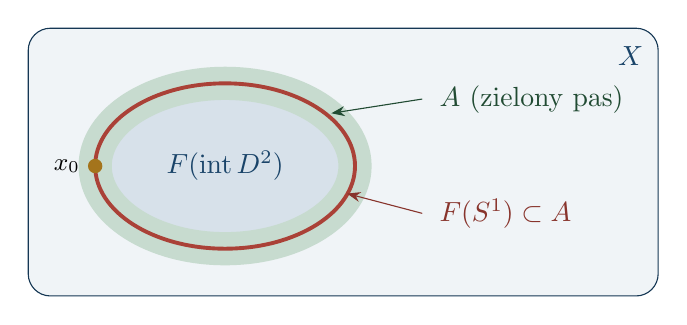
\begin{tikzpicture}[>=Stealth,line cap=round,line join=round]
 \filldraw[rounded corners=8pt,fill=manifoldblue!7,draw=manifoldblue!60!black]
  (0,0) rectangle (8,3.4);
 \fill[manifoldblue!18] (2.5,1.65) ellipse (1.65 and 1.05);
 \draw[manifoldgreen!28,line width=12pt] (2.5,1.65) ellipse (1.65 and 1.05);
 \draw[manifoldred,line width=1.4pt] (2.5,1.65) ellipse (1.65 and 1.05);
 \fill[manifoldgold!80!black] (.85,1.65) circle(2.6pt);
 \node[left,font=\small] at (.78,1.65) {$x_0$};
 \node[manifoldblue!75!black] at (2.5,1.65) {$F(\operatorname{int}D^2)$};
 \node[anchor=west,manifoldgreen!60!black] at (5.1,2.5) {$A$ (zielony pas)};
 \draw[->,manifoldgreen!60!black] (5,2.5)--(3.85,2.32);
 \node[anchor=west,manifoldred!80!black] at (5.1,1.05) {$F(S^1)\subset A$};
 \draw[->,manifoldred!80!black] (5,1.05)--(4.05,1.3);
 \node[manifoldblue!75!black] at (7.65,3.05) {$X$};
\end{tikzpicture}
\caption{Przykład odwzorowania względnego $(D^2,S^1,*)\to(X,A,x_0)$.
Czerwony obraz brzegu leży w zielonym pasie $A$, podczas gdy
obraz wnętrza dysku może wyjść poza $A$. W ogólnej definicji
nie wymaga się różnowartościowości $F$.}
\label{fig:pi-wzgledny-dysk}
\end{figure}

\begin{twierdzenie}[Długi ciąg homotopii pary]
\label{thm:les-pi}
Dla $x_0\in A\subseteq X$ otrzymujemy
naturalny ciąg
\begin{equation}\label{eq:les-pi}
 \cdots\to\pi_n(A,x_0)\xrightarrow{i_*}
 \pi_n(X,x_0)\xrightarrow{j_*}
 \pi_n(X,A,x_0)\xrightarrow{\partial}
 \pi_{n-1}(A,x_0)\xrightarrow{i_*}
 \pi_{n-1}(X,x_0)\to\cdots .
\end{equation}
Jest on dokładny: obraz każdej
strzałki to jądro następnej.
Odwzorowanie $\partial$ ogranicza
reprezentujący dysk do jego
wyróżnionej ściany $B$.
Na końcu ciągu występują
zbiory $\pi_1(X,A,x_0)$ i
$\pi_0(A),\pi_0(X)$; dokładność
oznacza tam przeciwobraz
wyróżnionego elementu.
\end{twierdzenie}
\begin{proof}
W modelu kostkowym $i_*$ jest
włączeniem $A\to X$, a $j_*$
traktuje odwzorowanie z całym brzegiem
w $x_0$ jako odwzorowanie względne.
Wzór $\partial[F]=[F|_B]$
jest poprawny, ponieważ
$\partial B\subset J$ i
$F(J)=x_0$. Homotopia
względna ogranicza się
do homotopii opartych
odwzorowań na $B$, więc
$\partial$ nie zależy
od reprezentanta.

Sprawdźmy trzy kolejne miejsca.
\emph{W $\pi_n(X)$.} Jeśli $f$ ma cały obraz w $A$, homotopia
$f_t(s',r)=f(s',(1-t)r+t)$ jest względną homotopią do stałej;
tutaj $s'\in I^{n-1}$, a $r$ jest ostatnią współrzędną.
Odwrotnie, niech $H(s',r,t)$ będzie względną homotopią
od $f$ do stałej. Ściana $g(s',t)=H(s',0,t)$ leży w $A$
i ma cały brzeg w $x_0$, więc reprezentuje element $\pi_n(A)$.
W kwadracie $(r,t)$ porównujemy drogi od $(0,0)$ do $(1,1)$:
dolny, a potem prawy bok oraz lewy, a potem górny bok.
Są homotopijne względem końców przez liniową interpolację w kwadracie.
Po złożeniu z $H$ dają odpowiednio $f$ i $g$ ze stałym dodatkowym
odcinkiem; na brzegu współrzędnych $s'$ wszystko pozostaje w $x_0$.
Stąd $[f]=i_*[g]$.

\emph{W $\pi_n(X,A)$.} Dysk
pochodzący z $\pi_n(X)$
ma stały brzeg, więc jego
$\partial$ jest zerem.
Jeśli natomiast brzeg
$F|_B:S^{n-1}\to A$ jest
zerowy w $\pi_{n-1}(A)$,
wybieramy jego wypełnienie
przez $D^n\to A$. Sklejenie
tego wypełnienia z $F$
wzdłuż wspólnego brzegu
daje oparte odwzorowanie
$S^n=D^n\cup_{S^{n-1}}D^n\to X$.
Po zapomnieniu drugiego
dysku jego obraz względny
jest klasą $[F]$.

\emph{W $\pi_{n-1}(A)$.} Brzeg
dysku względnego wypełnia
się w $X$, więc ginie
po włączeniu do $X$.
Jeśli oparte odwzorowanie
$S^{n-1}\to A$ jest
zerowe w $\pi_{n-1}(X)$,
jego homotopia do odwzorowania
stałego wyznacza wypełnienie
$D^n\to X$ i tym samym
klasę względną, której
brzeg jest daną klasą.
Te trzy rachunki powtarzają się w sąsiednich stopniach.
Na końcu ciągu element $\pi_1(X,A,x_0)$ jest drogą
od pewnego $a\in A$ do $x_0$, a $\partial$ przypisuje mu
składową $a$ w $A$. Trafia ona do wyróżnionej składowej $X$.
Odwrotnie, punkt tej składowej można połączyć drogą z $x_0$.
Jeśli $a$ leży w składowej $x_0$ już w $A$, dopinamy drogę
z $x_0$ do $a$ w $A$ i otrzymujemy pętlę w $X$ reprezentującą
daną klasę względną. To dowodzi dokładności także dla zbiorów wskazanych.
Wszystkie konstrukcje zachowują się przy składaniu z mapą par,
co daje naturalność ciągu.
\end{proof}

\begin{definicja}[Spójność homotopijna]
\index{spojnosc homotopijna@Spójność homotopijna}
\label{def:spojnosc-homotopijna}
Przestrzeń $X$ jest
\emph{$r$-spójna} ($r\geq0$),
jeśli jest łukowo spójna
i $\pi_i(X)=0$ dla $1\leq i\leq r$.
W szczególności $1$-spójna
oznacza jednospójną.
Para $(X,A)$ jest
\emph{$r$-spójna}, jeśli
każda składowa łukowa $X$
spotyka $A$ oraz
$\pi_i(X,A)=0$ dla
$1\leq i\leq r$ przy każdym wyborze punktu bazowego w $A$
(w stopniu $1$ jest to
trywialność zbioru
z wyróżnioną klasą).
\end{definicja}

Dokładność~\eqref{eq:les-pi}
pokazuje, że dla $r$-spójnej
pary włączenie $A\hookrightarrow X$
jest izomorfizmem na
$\pi_i$ dla $i<r$ oraz
surjekcją na $\pi_r$.
Wymiar komórek CW pozwoli
za chwilę uzyskać takie
zanikanie bez liczenia odwzorowań
pojedynczo.

\section{Homotopie na komórkach CW}
\label{sec:pi-n-cw}

W rozdziale o homologii komórki dawały
generatory grup łańcuchów. W homotopii
ich wymiary pozwalają \emph{usuwać
przeszkody do deformacji}. Żeby
deformować jedną komórkę bez psucia
tego, co zrobiliśmy na jej brzegu,
potrzebujemy przedłużania homotopii.

\begin{lemat}[Zwarte obrazy i homotopie w CW]
\label{lem:zwartosc-cw-pi}
Każdy zwarty podzbiór kompleksu CW leży w skończonym podkompleksie.
Ponadto odwzorowanie $H:X\times I\to Y$ jest ciągłe, jeśli jego złożenia
z każdym $\chi_\alpha\times\id_I:D^{d_\alpha}\times I\to X\times I$
są ciągłe, gdzie $\chi_\alpha$ są mapami charakterystycznymi komórek.
\end{lemat}
\begin{proof}
Gdyby zwarty zbiór $C$ spotykał nieskończenie wiele otwartych komórek,
wybralibyśmy z każdej z nich jeden punkt $c_\alpha\in C$.
Każda domknięta komórka spotyka tylko skończenie wiele spośród tych punktów.
Każdy podzbiór $E$ zbioru wybranych punktów ma więc domknięty
przeciwobraz przez każdą mapę charakterystyczną: jest to skończona
suma przeciwobrazów punktów w przestrzeni Hausdorffa.
Topologia słaba mówi, że $E$ jest domknięty w $X$.
Zatem zbiór wszystkich $c_\alpha$ jest domkniętym, dyskretnym
podzbiorem zwartego $C$, co jest niemożliwe, jeśli jest nieskończony.
Do skończenie wielu spotkanych komórek dołączamy ich ściany;
warunek skończoności domknięć i malejące wymiary dają skończony podkompleks.

Topologia słaba oznacza, że surjekcja
$q:\bigsqcup_\alpha D^{d_\alpha}\to X$ jest ilorazowa.
Iloczyn dowolnej mapy ilorazowej $q:E\to X$ z $\id_I$ też jest ilorazowy.
Aby to sprawdzić, niech przeciwobraz $W\subseteq X\times I$ będzie otwarty.
Dla $(x,t)\in W$ wybieramy zwarte otoczenie $J$ punktu $t$ w $I$
takie, że $\{x\}\times J\subset W$. Zbiór
$V=\{y:\{y\}\times J\subset W\}$ ma otwarty przeciwobraz przez $q$:
dla każdego $e$ nad $V$ skończone pokrycie zwartego $J$
prostokątami zawartymi w przeciwobrazie $W$ daje otoczenie $e$
o tej samej własności. Stąd $V$ jest otwarty i
$V\times\operatorname{int}_I J\subseteq W$ jest otoczeniem $(x,t)$.
To dowodzi tezy o iloczynie, a więc także kryterium ciągłości $H$.
\end{proof}

Z lematu wynika również rozszerzenie homologii komórkowej
z Rozdziału~\ref{ch:homologia-przestrzeni} na dowolne CW i pary CW.
Dla pary skończonych CW definiujemy najpierw
$C_\bullet^{\mathrm{CW}}(X,A)=C_\bullet^{\mathrm{CW}}(X)/C_\bullet^{\mathrm{CW}}(A)$:
jest to kompleks wolny na komórkach spoza $A$, z brzegiem modulo komórki $A$.
Krótki ciąg tych kompleksów daje długi ciąg homologii.
Naturalne porównanie ze zwykłym ciągiem pary i lemat pięciu
przenoszą izomorfizmy dla $A,X$ na grupy względne.
Każdy singularny łańcuch, jego brzeg oraz świadectwo homologiczności
są skończonymi sumami map zwartych sympleksów, więc mieszczą się
w skończonym podkompleksie. Cykl pochodzi z takiego podkompleksu,
a relacja między cyklami jest już prawdziwa w pewnym większym,
również skończonym. Tak samo jest dla skończonych sum komórek
i dla par: przecięcie skończonego podkompleksu z podkompleksem $A$
jest skończonym podkompleksem. Izomorfizmy dla modeli skończonych
są zgodne z włączeniami, bo pochodzą z naturalnych ciągów par.
Przechodzą więc na izomorfizmy dla całego CW.
Grupy łańcuchów komórkowych są przy tym \emph{sumami prostymi},
a nie iloczynami: każda kombinacja nadal ma skończony nośnik.

\begin{lemat}[Przedłużanie homotopii dla par CW]
\label{lem:hep-cw}
Niech $A\subseteq X$ będzie podkompleksem
CW. Jeśli $f:X\to Y$ i homotopia
$h:A\times I\to Y$ spełniają
$h(a,0)=f(a)$, to istnieje
$H:X\times I\to Y$ takie, że
$H(x,0)=f(x)$ oraz $H|_{A\times I}=h$.
W szczególności homotopię
zadaną na brzegu dołączonego
dysku można przedłużyć do
całego dysku.
\end{lemat}
\begin{proof}
Najpierw rozważmy jedną komórkę
$D^k$, której brzeg $S^{k-1}$
leży w już zbudowanej części.
Na
\[
 (D^k\times\{0\})\cup
 (S^{k-1}\times I)
\subset D^k\times I
\]
mamy dane: $f$ na dole
i homotopię $h$ na boku.
Ta podprzestrzeń jest
retraktem całego cylindra.
Można to zobaczyć jawnie:
pisząc $r=\|x\|$ i
\[
 \lambda(x,t)=
 \min\left\{\frac1r,\frac2{2-t}\right\},
 \qquad
 R(x,t)=\bigl(\lambda x,\,
                  2-\lambda(2-t)\bigr),
\]
przy $r=0$ przyjmujemy
$1/r=+\infty$. Dla $r\leq1/2$ minimum wynosi $2/(2-t)$,
więc wzór jest ciągły także przy $r=0$. Wartość
$R(x,t)$ leży albo na boku
$\|\lambda x\|=1$, albo
na dole z drugą współrzędną
równą $0$. Jeśli $t=0$
lub $r=1$, mamy $\lambda=1$,
więc $R$ pozostawia dane
punkty nieruchome.
Złożenie danych z $R$
przedłuża homotopię
na $D^k\times I$.

Dołączajmy teraz komórki
$X\setminus A$ według
wymiarów. Na każdym kroku
stosujemy poprzednią
konstrukcję na wszystkich
dyskach danego wymiaru;
na ich brzegach odwzorowania
już się zgadzają. Ponieważ
topologia CW jest zadana
przez odwzorowania charakterystyczne,
sklejone homotopie są
ciągłe. Dla nieskończenie wielu komórek uzasadnieniem ciągłości
z parametrem czasu jest Lemat~\ref{lem:zwartosc-cw-pi},
zastosowany do wszystkich map $D^k\times I\to Y$.
Dla $0$-komórek wybieramy homotopię stałą równą wartości $f$;
wzór na $R$ jest potrzebny dla $k\geq1$.
\end{proof}

\begin{twierdzenie}[Przybliżenie komórkowe]
\label{thm:przyblizenie-komorkowe}
Każde odwzorowanie $f:X\to Y$ kompleksów CW
jest homotopijne z odwzorowaniem
\emph{komórkowym}, czyli takim,
które spełnia
$f(X^k)\subseteq Y^k$ dla
każdego $k$. Jeśli na
podkompleksie $A\subseteq X$
odwzorowanie już jest komórkowe,
homotopię można wybrać
stałą na $A$.
\end{twierdzenie}
\begin{proof}
Wyjaśnijmy lokalny krok geometryczny. Niech
$u:D^k\to Y^m$ wysyła brzeg do $Y^{k-1}$, gdzie $m>k$.
Obraz jest zawarty w skończonym podkompleksie na mocy
Lematu~\ref{lem:zwartosc-cw-pi}. W jednej otwartej $m$-komórce
używamy współrzędnych $\operatorname{int}D^m$ i oznaczamy przez $v$
współrzędnościowy zapis $u$ na otwartym przeciwobrazie tej komórki.
Wybierzmy $0<a<b<c<1$. Zbiór $K=v^{-1}(\overline B_b)$
jest zwarty i leży we wnętrzu $D^k$: obraz $\overline B_b$
jest zwarty i domknięty w przestrzeni Hausdorffa $Y$.
Wybieramy skończone otoczenie wielościenne $P$ zbioru $K$
takie, że $K\subset\operatorname{int}P\subset P\subset v^{-1}(B_c)$.
Można je uzyskać jako sumę domkniętych kostek dostatecznie drobnej siatki
spotykających $K$. Triangulujemy $P$ i przez interpolację wartości $v$
w wierzchołkach dostajemy odcinkowo afiniczne $w$ z
$\|w-v\|<\varepsilon$, gdzie $\varepsilon<\min(b-a,1-c)$.
Istnienie takiego przybliżenia wynika z jednostajnej ciągłości $v$ na $P$:
na każdym małym sympleksie interpolujemy wartości różniące się o mniej niż $\varepsilon$.

Niech $\eta:D^k\to[0,1]$ będzie ciągła, równa $1$ na $K$
i $0$ poza $\operatorname{int}P$. Na $P$ stosujemy homotopię
$v_t=v+t\eta(w-v)$, a poza $P$ nic nie zmieniamy.
Wszystkie wartości pozostają we wnętrzu komórki i homotopia nie rusza brzegu dysku.
Poza $K$ mamy $\|v\|>b$, więc $\|v_t\|>a$.
W $K$ końcowe odwzorowanie jest równe $w$.
Jego obraz jest zawarty w skończonej sumie podprzestrzeni afinicznych
wymiaru co najwyżej $k<m$, która nie zawiera otwartej kuli $B_a$.
Istnieje więc $z\in B_a$ pominięty przez całe nowe odwzorowanie.

Promieniowa retrakcja $D^m\setminus\{z\}$ na $\partial D^m$
zostawia brzeg nieruchomy, więc po sklejeniu komórki daje homotopię
usuwającą jej wnętrze z obrazu $u$. Ciągłość z parametrem czasu
wynika z ilorazowego kryterium z poprzedniego lematu.
Usuwamy kolejno komórki najwyższego wymiaru i schodzimy z wymiarem do $k$.
Pracujemy w skończonym podkompleksie zawierającym obraz i domknięcia
spotkanych komórek, zatem proces kończy się po skończenie wielu krokach.

Zaczynamy od $X^0$:
obraz każdego wierzchołka
przesuwamy do odpowiedniego
wierzchołka w jego składowej
$Y$, a na $A$ niczego
nie zmieniamy. Załóżmy
indukcyjnie, że
$f(X^{k-1})\subseteq Y^{k-1}$.
Dla każdej $k$-komórki
stosujemy lokalny krok
do jej odwzorowania
charakterystycznego:
usuwamy po kolei obrazy
komórek celu o wymiarach
$m>k$, zachowując
jej brzeg. Dostajemy
odwzorowanie tej komórki do
$Y^k$. Dzięki
Lematowi~\ref{lem:hep-cw}
homotopię na dotychczas
zbudowanej części
przedłużamy na całe $X$
i przechodzimy do
następnego wymiaru.
Podane kroki wykonuje
się względnie $A$.
Etapowi wymiaru $k$ przydzielamy przedział
$[1-2^{-k},1-2^{-k-1}]$, a w chwili $1$ bierzemy odwzorowanie końcowe.
Każdy ustalony szkielet pozostaje nieruchomy po zakończeniu swojego etapu.
Na każdym $D^k\times I$ mamy więc skończenie wiele sklejonych homotopii
i stały odcinek końcowy. Lemat~\ref{lem:zwartosc-cw-pi}
zapewnia ciągłość całej homotopii, także w chwili $1$.
\end{proof}

\begin{uwaga}[Przybliżenie w równych wymiarach]
\label{rem:przyblizenie-rowne-wymiary}
Ta sama lokalna konstrukcja dla $k=m$ pozwala wybrać $z\in B_a$
poza obrazami ścian triangulacji $P$ i tych $m$-sympleksów,
na których $w$ ma rząd mniejszy od $m$. Jest to skończona suma
zbiorów o wymiarze mniejszym od $m$. Każdy przeciwobraz $z$
leży wtedy we wnętrzu jednego sympleksu, gdzie $w$ jest afinicznym homeomorfizmem.
Przeciwobrazów jest skończenie wiele, a każdy ma znak wyznacznika $+1$ lub $-1$.
Możemy wokół $z$ wybrać małą kulę, której przeciwobrazy są rozłącznymi
dyskami, odwzorowanymi homeomorficznie na tę kulę.
To wynika również ze zwartości: poza małymi otoczeniami znalezionych
przeciwobrazów obraz omija całe dostatecznie małe otoczenie $z$.
Ten wariant będzie użyty w dowodzie o pierwszych komórkach.
\end{uwaga}

\begin{wniosek}[Szkielet widziany przez $\pi_i$]
\label{cor:pi-szkielety}
Dla kompleksu CW $X$ para
$(X,X^n)$ jest $n$-spójna.
Włączenie $X^n\hookrightarrow X$
daje więc izomorfizm na
$\pi_i$ dla $i<n$
i surjekcję dla $i=n$.
Jeśli $1\leq i<k$, to
$\pi_i(S^k)=0$.
\end{wniosek}
\begin{proof}
Reprezentant klasy
$\pi_i(X,X^n)$ jest
odwzorowaniem $(D^i,\partial D^i)\to
(X,X^n)$, gdzie $i\leq n$.
Najpierw przybliżamy komórkowo mapę brzegu do $X^n$,
zachowując punkt bazowy, i przedłużamy tę homotopię na dysk
Lematem~\ref{lem:hep-cw}. Dopiero teraz brzeg jest komórkowy,
więc względne przybliżenie na dysku przesuwa cały obraz do
$X^i\subseteq X^n$. Klasa względna znika.
Każda składowa $X$ zawiera wierzchołek: punkt komórki można
połączyć z jej brzegiem i powtarzać to w malejących wymiarach.
To daje także stwierdzenie o składowych i przypadek $n=0$.
Długi ciąg~\eqref{eq:les-pi}
daje twierdzenie o
włączeniu szkieletu.
Sfera $S^k$ ma strukturę CW
z jednym wierzchołkiem
i jedną $k$-komórką,
więc jej $i$-szkielet
jest punktem dla $0\leq i<k$.
Każde oparte odwzorowanie
$S^i\to S^k$ jest
homotopijne do odwzorowania
komórkowego i wtedy
jego obraz jest punktem.
\end{proof}

\begin{stwierdzenie}[Wyższe grupy i nakrycia]
\label{prop:pi-n-nakrycie}
Jeśli $p:\widetilde X\to X$
jest nakryciem, $\widetilde x_0$
leży nad $x_0$, to
\[
 p_*:\pi_n(\widetilde X,\widetilde x_0)
 \xrightarrow{\ \cong\ }
 \pi_n(X,x_0)\qquad(n\geq2).
\]
\end{stwierdzenie}
\begin{proof}
Sfera $S^n$ dla $n\geq2$
jest jednospójna na mocy
Wniosku~\ref{cor:pi-szkielety}
(dla $n=2$ znika $\pi_1$,
a dla większych wymiarów
również). Każde oparte
odwzorowanie $S^n\to X$ podnosi
się więc jednoznacznie
po wskazaniu obrazu
punktu bazowego,
zgodnie z kryterium
z Twierdzenia~\ref{thm:kryterium-podnoszenia}.
Daje to surjektywność $p_*$.
Jeśli dwa podniesienia
po zrzutowaniu są
homotopijne przez odwzorowania oparte,
ich homotopię
$S^n\times I\to X$ podnosimy z kryterium podnoszenia:
$S^n\times I$ jest łukowo i lokalnie łukowo spójna oraz jednospójna,
bo retrahuje się na $S^n$. Ustalamy obraz $(\ast,0)$.
Ścieżka punktu bazowego leży w dyskretnym włóknie, więc jest stała,
a ograniczenie do $S^n\times\{0\}$ jest zadanym podniesieniem.
Jednoznaczność podnoszenia
sprawia, że na końcu
otrzymujemy drugie
podniesienie, ponieważ
oba zgadzają się w
punkcie bazowym.
To daje iniektywność.
\end{proof}

\begin{przyklad}[Okrąg i torus nie mają wyższych $\pi_n$]
\label{prz:pi-torus}
Nakrycia $\R\to S^1$ i
$\R^2\to T^2=S^1\times S^1$
mają ściągalne przestrzenie
całkowite. Zatem dla $n\geq2$
\[
 \pi_n(S^1)=0,\qquad
 \pi_n(T^2)=0.
\]
Jednocześnie
$H_2(T^2)=\Z$ z
Przykładu~\ref{prz:homologia-cw-torus}.
Już tu widać, że w
przestrzeni z nietrywialną
$\pi_1$ wyższa homologia
nie musi być obrazem
wyższej grupy homotopii.
\end{przyklad}

\section{Pierwsze odwzorowanie Hurewicza: od pętli do cykli}
\label{sec:hurewicz-jeden}

\begin{twierdzenie}[Hurewicz w stopniu pierwszym]
\label{thm:hurewicz-h1}
Dla przestrzeni łukowo spójnej $X$
odwzorowanie przypisujące opartej pętli
jej klasę singularnego
$1$-cyklu indukuje naturalny
izomorfizm
\[
 h_1:\pi_1(X,x_0)_{\mathrm{ab}}
 =\pi_1(X,x_0)/
 [\pi_1(X,x_0),\pi_1(X,x_0)]
 \xrightarrow{\ \cong\ }H_1(X;\Z).
\]
\end{twierdzenie}
\begin{proof}
Pętla $\ell:I\to X$ ma
$\partial\ell=[x_0]-[x_0]=0$.
Złożenie dwóch pętli
ma tę samą klasę homologii
co suma ich łańcuchów:
singularny $2$-sympleks, którego boki
przebiegają $\ell_1$, $\ell_2$ i ich złożenie, ma
brzeg $\ell_1+\ell_2-
(\ell_1*\ell_2)$
(z odpowiednią
parametryzacją boków).
Homotopia oparta pętli daje homologiczne cykle przez operator pryzmatyczny
z Twierdzenia~\ref{thm:homotopia-singularna}.
Zatem $[\ell]\mapsto
[\ell]_{H_1}$ jest
homomorfizmem do grupy
abelowej i zabija komutatory.

Skonstruujemy odwrotność.
Dla każdego $x\in X$
wybierzmy drogę $u_x$
od $x_0$ do $x$,
przy czym $u_{x_0}$
jest drogą stałą.
Singularnej krawędzi
$\sigma:x\to y$
przypiszmy w
$\pi_1(X,x_0)_{\mathrm{ab}}$
klasę pętli
\[
 L(\sigma)
 =[u_x*\sigma*\bar u_y].
\]
Niech $\tau:\Delta^2\to X$,
a $x_0',x_1',x_2'$
będą obrazami jej
wierzchołków.
Pętla złożona z boków
$\tau_{01}*\tau_{12}*
\bar\tau_{02}$ jest
zerowa w $\pi_1(X,x_0')$,
gdyż wypełnia ją
sam trójkąt $\tau$.
Po doprowadzeniu jej
do bazy drogami $u_{x_i'}$
otrzymujemy
\[
 L(\partial\tau)
 =L(\tau_{12})-L(\tau_{02})
  +L(\tau_{01})=0
 \quad\text{w }\pi_1(X,x_0)_{\mathrm{ab}}.
\]
Przez liniowość $L$
zeruje więc wszystkie
singularne brzegi
$2$-wymiarowe.
Na cyklach $z\in C_1(X)$
daje homomorfizm
$\bar L:H_1(X)\to
\pi_1(X,x_0)_{\mathrm{ab}}$.

Dla opartej pętli
$\ell$ mamy $L(\ell)=[\ell]$,
więc $\bar Lh_1=\id$.
W drugą stronę,
w homologii
obraz cyklu
$z=\sum m_\sigma\sigma$
rozwija się na
sumę łańcuchów $u_x$, samych krawędzi i $-u_y$,
z dokładnością do brzegów $2$-łańcuchów.
Pojedyncze $u_x$ zwykle nie są cyklami, więc nie przypisujemy
im osobnych klas w $H_1$. Rachunek przeprowadzamy w $C_1(X)/\operatorname{im}\partial_2$.
Tożsamość dla złożenia dróg wynika z trójkąta użytego na początku,
także gdy ich końce są różne; droga odwrotna daje ujemny łańcuch
modulo brzegi, bo droga złożona z własną odwrotnością jest homotopijna do stałej.
Współczynnik przy
każdej pomocniczej
drodze $u_x$ jest
równy minus współczynnikowi
przy $[x]$ w $\partial z$,
a zatem zerowy.
Pozostaje klasa
samego $z$ w $H_1(X)$;
formalnie używamy
homologii złożenia
dróg udowodnionej
na początku. Stąd
$h_1\bar L=\id$
i oba odwzorowania są
odwrotne.
\end{proof}

\begin{przyklad}[Od wolnej grupy do liczby pętli]
Bukiet $r$ okręgów ma
grupę podstawową
$F_r$ z
Przykładu~\ref{prz:pi1-dwa-okregi}
(dla $r=2$ rachunek
podano tam wprost).
Po narzuceniu
przemienności generatorów
$F_r^{\mathrm{ab}}\cong\Z^r$,
zgodnie z
Przykładem~\ref{prz:homologia-bukiet}.
Homologia pamięta tu
liczbę niezależnych
kierunków, ale nie
kolejność, w jakiej
przebywamy pętle.
\end{przyklad}

\section{Twierdzenie Whiteheada}
\label{sec:whitehead}

Równość wszystkich grup $\pi_n$
nie oznacza automatycznie, że
dowolne odwzorowanie przestrzeni
topologicznych ma homotopijną
odwrotność. Dla kompleksów CW
komórki pozwalają jednak
przekształcić informację
o sferach w deformację
całej przestrzeni.

\begin{definicja}[Słaba równoważność homotopijna]
\index{slaba rownowaznosc homotopijna@Słaba równoważność homotopijna}
\label{def:slaba-rownowaznosc}
Odwzorowanie $f:X\to Y$ jest
\emph{słabą równoważnością
homotopijną}, jeśli daje
bijekcję $\pi_0(X)\to\pi_0(Y)$
i dla wszystkich punktów
bazowych $x\in X$ oraz
wszystkich $n\geq1$
izomorfizmy
$f_*:\pi_n(X,x)\to
\pi_n(Y,f(x))$.
\end{definicja}

\begin{lemat}[Ściskanie komórek]
\label{lem:kompresja-cw}
Niech $(K,L)$ będzie parą CW,
a $B\subseteq Y$ niepustą
podprzestrzenią. Załóżmy, że
każda składowa łukowa $Y$ spotyka
$B$ oraz wszystkie grupy
$\pi_k(Y,B,b)$ dla
$k\geq1$ i $b\in B$
są trywialne (dla $k=1$ chodzi o zbiór z wyróżnioną klasą). Wówczas
każde odwzorowanie par
$F:(K,L)\to(Y,B)$
jest homotopijne
\emph{względem $L$}
z odwzorowaniem o obrazie w $B$.
\end{lemat}
\begin{proof}
Dla $0$-komórek $K\setminus L$
wybieramy drogi z ich obrazów
do $B$. Homotopia przesuwa
te obrazy do $B$ i jest
stała na $L$.

Załóżmy, że tak zrobiliśmy
na wszystkich komórkach
o wymiarze mniejszym od $k$.
Dla dołączonej $k$-komórki
odwzorowanie charakterystyczne
daje parę
$(D^k,S^{k-1})\to(Y,B)$.
Przy $k\geq1$ jej klasa
w $\pi_k(Y,B)$ jest zerowa.
Znaczy to, że można
deformować dysk do $B$,
pozwalając początkowo
brzegowi poruszać się w $B$.
Wyjaśnijmy, jak unieruchomić brzeg. Niech
$G:D^k\times I\to Y$ będzie względną homotopią do stałej,
z $G_0=F$ i $G_t(S^{k-1})\subset B$.
Połóżmy $a_t=1-t/2$ i dla $x=ru$ określmy
\[
 K_t(ru)=
 \begin{cases}
 G_t(ru/a_t),&r\leq a_t,\\
 G_{2(1-r)}(u),&a_t\leq r\leq1.
 \end{cases}
\]
Na $r=a_t$ oba wzory dają $G_t(u)$, na $r=1$ mamy stale $F(u)$,
a dla $t=0$ otrzymujemy $F$. Ciągłość przy zanikającym kołnierzu
wynika z ciągłości $G$; dla $t=1$ cały obraz leży w $B$.
Tak dostajemy deformację względem całego brzegu, a nie jedynie
homotopię, która pozwala mu przesuwać się w $B$.
Wykonujemy je na
wszystkich $k$-komórkach
równocześnie.
Lemat~\ref{lem:hep-cw}
przedłuża otrzymaną
homotopię do reszty
$K$, bez ruszania $L$.
Indukcja usuwa obrazy
wszystkich komórek
spoza $L$ z $Y\setminus B$.
Dla nieskończonego CW
przeznaczamy na etap $k$
coraz krótszy przedział
czasu kończący się w $1$.
Każdy ustalony szkielet staje się w końcu nieruchomy.
Ograniczenie do każdej domkniętej komórki, wraz z całym przedziałem czasu,
jest skończonym sklejeniem ciągłych homotopii i stałego końca.
Lemat~\ref{lem:zwartosc-cw-pi} daje ciągłość także w chwili $1$.
\end{proof}

\begin{twierdzenie}[Whitehead]
\label{thm:whitehead}
Słaba równoważność homotopijna
$f:X\to Y$ między kompleksami
CW jest równoważnością
homotopijną. Jeśli
$i:X\hookrightarrow Y$
jest włączeniem podkompleksu
i indukuje izomorfizmy
wszystkich $\pi_n$ oraz
bijekcję na $\pi_0$, to
$X$ jest silnym retraktem
deformacyjnym $Y$.
\end{twierdzenie}
\begin{proof}
Jeśli $X=\varnothing$, bijekcja na składowych wymusza $Y=\varnothing$
i teza jest natychmiastowa. Dalej zakładamy $X\ne\varnothing$.
Zacznijmy od włączenia.
W długim ciągu~\eqref{eq:les-pi}
pary $(Y,X)$ znajdują się
fragmenty
\[
 \pi_n(X)\xrightarrow[\cong]{i_*}
 \pi_n(Y)\longrightarrow
 \pi_n(Y,X)\longrightarrow
 \pi_{n-1}(X)
 \xrightarrow[\cong]{i_*}
 \pi_{n-1}(Y).
\]
Dokładność wymusza
$\pi_n(Y,X)=0$ dla
wszystkich $n\geq2$.
Dla stopnia $1$ warto użyć dróg, ponieważ nie jest to już ciąg grup.
Droga względna od $a\in X$ do $x_0$ ma oba końce w jednej składowej $X$,
gdyż $\pi_0(X)\to\pi_0(Y)$ jest injekcją. Dopinamy drogę
od $x_0$ do $a$ w $X$, otrzymując pętlę w $Y$.
Surjektywność $\pi_1(X)\to\pi_1(Y)$ pozwala zastąpić ją pętlą w $X$.
Każda taka droga jest trywialna względnie $X$, więc $\pi_1(Y,X)$
ma tylko wyróżniony element. Każda składowa $Y$ spotyka $X$,
bo odwzorowanie na $\pi_0$ jest także surjekcją.
Lemat~\ref{lem:kompresja-cw}
zastosowany do
$F=\id_Y:(Y,X)\to(Y,X)$
daje homotopię nieruchomą
na $X$, prowadzącą od
$\id_Y$ do odwzorowania
$r:Y\to X$.
Ponieważ $r|_X=\id_X$,
jest to silna retrakcja
deformacyjna.

Niech teraz $f$ będzie
dowolną słabą równoważnością
CW. Twierdzenie
\ref{thm:przyblizenie-komorkowe}
pozwala zastąpić ją
odwzorowaniem komórkowym $f'\simeq f$.
Zmiana punktu bazowego wzdłuż tej homotopii pokazuje,
że $f'$ nadal jest słabą równoważnością.
Utwórzmy jego
\emph{cylinder odwzorowania}
\[
 M_{f'}=(X\times I)\sqcup Y/
       \bigl((x,1)\sim f'(x)\bigr).
\]
Cylinder ma strukturę CW: poza komórkami $Y$ bierzemy dolne
komórki $e^k\times\{0\}$ i komórki $e^k\times(0,1)$ wymiaru $k+1$.
Brzeg każdej z tych ostatnich składa się z dołu, boków nad
brzegiem $e^k$ i góry odwzorowanej przez $f'$ do $Y^k$.
Komórkowość $f'$ zapewnia zgodność wymiarów, a topologia
ilorazowa i Lemat~\ref{lem:zwartosc-cw-pi} dają topologię słabą.
Dolna kopia $X=X\times\{0\}$ jest więc podkompleksem $M_{f'}$.
Zwijając każdy odcinek
$\{x\}\times I$ do
$f'(x)\in Y$, otrzymujemy
retrakcyjną deformację
$M_{f'}\to Y$.
Złożenie włączenia
$X\hookrightarrow M_{f'}$
z tą retrakcją to $f'$.
Ponieważ $f'_*$ i
retrakcyjne odwzorowanie na $Y$
indukują izomorfizmy
na $\pi_n$, również
włączenie $X\hookrightarrow
M_{f'}$ je indukuje.
Pierwsza część dowodu
ściska więc $M_{f'}$
do $X$. Oznaczmy dolne włączenie przez $j$, włączenie $Y$ do cylindra przez $i$,
a retrakcje na $X,Y$ odpowiednio przez $s,r$.
Wtedy $f'=rj$, a odwrotnością homotopijną jest $g=si$:
$gf'=sirj\simeq sj=\id_X$ oraz $f'g=rjsi\simeq ri=\id_Y$.
Ponieważ $f\simeq f'$, to samo $g$ jest odwrotnością homotopijną $f$.
\end{proof}

\begin{figure}[!htbp]
\centering
\begin{tikzpicture}[>=Stealth,line cap=round,line join=round]
 \fill[manifoldblue!10]
  (0,0)--(4.1,0)--(4.35,2.0)--(.25,2.0)--cycle;
 \draw[manifoldblue!70!black,thick]
  (0,0)--(4.1,0)--(4.35,2.0)--(.25,2.0)--cycle;
 \foreach \x in {.7,1.8,2.9,3.7}{
  \draw[manifoldblue!35] (\x,.07)--({\x+.23},1.94);
 }
 \fill[manifoldgreen!18]
  (-.38,2.0) rectangle (4.86,2.5);
 \draw[manifoldgreen!70!black,thick]
  (-.38,2.0) rectangle (4.86,2.5);
 \node at (2.2,2.25) {$Y$};
 \node[below] at (2.08,0) {$X\times\{0\}$};
 \node[manifoldblue!70!black] at (2.2,1.02)
  {$X\times I$};
 \node[manifoldred!85!black,above]
  at (2.2,2.62) {$(x,1)\sim f'(x)$};
 \draw[->,manifoldred,thick]
  (3.35,1.48)--(3.35,2.2)
  node[midway,right=3pt] {$r$};
 \node[font=\small,align=left,anchor=west,text width=4.8cm]
  at (5.15,1.15)
  {Cylinder zwija się na $Y$.
   Gdy $f'$ jest słabą równoważnością,
   poprzednia część dowodu zwija go
   również na dolną kopię $X$.};
\end{tikzpicture}
\caption{Cylinder odwzorowania zamienia
odwzorowanie $f':X\to Y$ na włączenie
podkompleksu $X\hookrightarrow M_{f'}$.
Rysunek pokazuje mechanizm dowodu
twierdzenia Whiteheada.}
\label{fig:cylinder-whiteheada}
\end{figure}

\begin{uwaga}[Zakres twierdzenia]
Sprawdzenie tylko $\pi_1$
i kilku pierwszych grup
$\pi_n$ nie wystarcza
do zastosowania Whiteheada:
założenie dotyczy
\emph{każdego} $n$.
Również samo podobieństwo
grup homologii dwóch
przestrzeni nie wskazuje
jeszcze odwzorowania, które
mogłoby być równoważnością.
Niżej wyprowadzimy
użyteczne kryterium
homologiczne przy
dodatkowej jednospójności.
\end{uwaga}

\section{Odwzorowanie Hurewicza i pierwszy niezerowy wymiar}
\label{sec:hurewicz-wyzszy}

\begin{definicja}[Odwzorowanie Hurewicza]
\index{odwzorowanie hurewicza@Odwzorowanie Hurewicza}
\label{def:mapa-hurewicza}
Homologia $H_n(S^n;\Z)$
jest izomorficzna z $\Z$
na mocy
Twierdzenia~\ref{thm:homologia-sfer}.
Wybierzmy generatory zgodnie z orientacjami dysków i ich brzegów,
tak aby $\delta[D^n,S^{n-1}]=[S^{n-1}]$.
Dla $n\geq2$ określamy
\[
 h_n:\pi_n(X,x_0)\longrightarrow H_n(X;\Z),
 \qquad h_n([f])=f_*[S^n].
\]
Dla pary $(X,A)$ bierzemy
analogicznie generator
$[D^n,S^{n-1}]
\in H_n(D^n,S^{n-1})$ i
kładziemy
\[
 h_n^{\mathrm{rel}}([F])
 =F_*[D^n,S^{n-1}]
 \in H_n(X,A).
\]
W stopniu $1$ dla przestrzeni używamy homomorfizmu
$\pi_1(X)\to\pi_1(X)_{\mathrm{ab}}\xrightarrow{h_1}H_1(X)$.
Względny homomorfizm określamy tutaj dla $n\geq2$;
zbiór $\pi_1(X,A)$ nie jest w ogólności grupą.
\end{definicja}

Homotopie oparte są w
szczególności zwykłymi
homotopiami odwzorowań, więc
$h_n$ jest dobrze
określone dzięki
Twierdzeniu~\ref{thm:homotopia-singularna}.
Odwzorowanie jest homomorfizmem:
sklejanie dwóch połówek
sfery odpowiada sumie
ich klas fundamentalnych.
Dokładniej, sklejanie jest złożeniem mapy ściskającej równik
$S^n\to S^n\vee S^n$ z $f\vee g$. Mapa ściskająca posyła
generator na sumę dwóch generatorów: rzut na każdy składnik
ma stopień $+1$, co widać z klasy orientacji odpowiedniej półkuli
i naturalności odwzorowania łączącego dla dysku i brzegu.
Względnie używamy kostki podzielonej na dwie połowy w pierwszej współrzędnej.
Po zorientowaniu obu połówek zgodnie z całą kostką ich wewnętrzne
ściany kasują się; obraz łańcucha fundamentalnego jest sumą obu obrazów.
To daje również homomorfizm względny. Naturalność wynika od razu ze składania map.

Do dowodu potrzebujemy
przeliczyć grupy homotopii
prostych modeli komórkowych.
Najważniejszy jest
następujący krok: w
pierwszym nowym wymiarze
komórki są niezależne,
a komórki o wymiar
wyższym wprowadzają
relacje.

\begin{lemat}[Pierwsze komórki i ich relacje]
\label{lem:pierwsze-komorki-pi}
Niech $A$ będzie jednospójnym
podkompleksem CW kompleksu $Z$.
Załóżmy, że wszystkie komórki
$Z\setminus A$ mają wymiar
co najmniej $n\geq2$.
Oznaczmy przez $I_n$
zbiór nowych $n$-komórek.
Wtedy
\[
 \pi_n(Z^n\cup A,A)
 \cong\bigoplus_{\alpha\in I_n}\Z[e_\alpha^n]
 \xrightarrow[\cong]{\ h_n^{\mathrm{rel}}\ }
 H_n(Z^n\cup A,A).
\]
Po dołączeniu $(n+1)$-komórek
obie grupy otrzymujemy
z tej wolnej grupy przez
te \emph{same} relacje:
obraz brzegu odwzorowania
dołączającego $S^n\to
Z^n\cup A$. Komórki
o wymiarach co najmniej
$n+2$ nie zmieniają
tych grup.
\end{lemat}
\begin{proof}
Niech $W=Z^n\cup A$ oraz $W'=Z^{n+1}\cup A$.
Przestrzeń $W$ jest jednospójna: do jednospójnego $A$
dołączamy tylko komórki wymiaru co najmniej $2$, co nie tworzy
nowych pętli (lokalny krok przybliżenia komórkowego przesuwa pętlę do $A$).
W szczególności także $\pi_2(W,A)$ jest abelowa, bo z ciągu pary
jest ilorazem abelowej $\pi_2(W)$ przy $\pi_1(A)=0$.
Możemy więc mówić o homomorfizmie z wolnej grupy abelowej
również w przypadku $n=2$.
Po zwinięciu $A$
otrzymujemy bukiet
$\bigvee_{\alpha\in I_n}S^n$.
Względna homologia
$H_n(W,A)$ jest
wolna na komórkach
na mocy
Twierdzenia~\ref{thm:warstwa-komorek}
i rozszerzenia na pary CW po Lemacie~\ref{lem:zwartosc-cw-pi};
to jeszcze nie jest
argument o homotopii,
więc rozpiszmy go
osobno.

Każdą mapę charakterystyczną nowej komórki opieramy w $x_0$
przez dołączenie drogi w $A$ do obrazu wybranego punktu jej brzegu.
Wybór drogi nie zmienia klasy, bo $A$ jest jednospójna.
Tak rozumiemy symbole $[e_\alpha^n]$ po stronie homotopii.
Weźmy teraz odwzorowanie względne
$F:(D^n,S^{n-1},*)\to(W,A,x_0)$.
Zwarty obraz spotyka
tylko skończenie wiele
otwartych komórek.
W każdej z nowych $n$-komórek stosujemy przybliżenie
z Uwagi~\ref{rem:przyblizenie-rowne-wymiary}, nieruchome przy $S^{n-1}$.
Wybieramy regularny punkt $z_\alpha$ poza obrazami ścian triangulacji.
Ma on skończenie wiele przeciwobrazów; na małych otoczeniach
$F$ jest afinicznym homeomorfizmem o znaku $+1$ lub $-1$.
Wybierzmy wokół $z_\alpha$ małą kulę. Jej przeciwobrazy są rozłącznymi
dyskami $D_j$, a poza nimi $F$ omija tę kulę.
Parametryzując $D_j$ przez odwrotność lokalnej mapy afinicznej,
otrzymujemy dokładnie lokalny fragment mapy charakterystycznej;
ujemny znak odpowiada odbiciu pierwszej współrzędnej, czyli odwrotności w grupie. Po usunięciu
środków każda komórka
promieniowo zwija się
na swój brzeg w $A$;
zatem odwzorowanie na dopełnieniu
małych dysków możemy
przesunąć do $A$.
Przedłużamy tę deformację na $D_j$ przez rozszerzanie ich obrazów
od małej kuli do całej komórki, zostawiając zgodność na wspólnych brzegach.
Połączmy małe dyski i punkt bazowy drzewem łuków w ich dopełnieniu.
Rozcinając wzdłuż cienkich pasów tego drzewa, przedstawiamy dysk
jako sumę dysków z doprowadzeniem do bazy; pozostałe części mają obraz w $A$
i reprezentują zero względne. Takie rozcięcie realizuje kolejno
kostkowe dodawanie z Definicji~\ref{def:pi-wzgledne}:
wewnętrzny pas ma obraz w $A$ i można go przesuwać podczas homotopii względnej.
Zmiana drogi doprowadzającej modyfikuje składnik przez pętlę w $A$.
Ponieważ $\pi_1(A)=0$, te zmiany nie wpływają na klasę.
Ostatecznie $[F]$ jest sumą klas charakterystycznych dysków
$e_\alpha^n$, z ich znakami. Każda suma jest skończona.
To dowodzi surjektywności
odwzorowania od wolnej grupy
na nowych komórkach
do $\pi_n(W,A)$.
Obrazy tych generatorów
przez $h_n^{\mathrm{rel}}$
tworzą bazę
$H_n(W,A)$. Gdyby ich
kombinacja dawała
zerową klasę względnej
homotopii, jej obraz
homologiczny również
byłby zerowy; niezależność
bazy wymusza wszystkie
współczynniki równe $0$.
Mamy więc izomorfizm.

Niech teraz dołączamy dyski $D^{n+1}_\beta$, otrzymując $W'$.
Każdą mapę $D^n\to W'$ względnie $A$ przesuwamy do $W$
przez lokalne usuwanie punktów w komórkach wymiaru $n+1$.
Włączenie indukuje więc surjekcję na $\pi_n$.
Relację od $\varphi_\beta:S^n\to W$ rozumiemy jako jej obraz
przez $\pi_n(W)\to\pi_n(W,A)$.
Ich odwzorowania charakterystyczne
dają oczywiste relacje:
brzeg każdego takiego
dysku staje się zerem
w $\pi_n(W',A)$.
Dlaczego nie pojawiają
się inne relacje?
Homotopię względną
między dwoma sumami
$n$-dysków przedstawiamy
na $D^n\times I$.
Uwaga~\ref{rem:przyblizenie-rowne-wymiary}, zastosowana do cylindra
triangulowanego jako $(n+1)$-dysk i nieruchomo na całym jego brzegu,
zapewnia, że przeciwobrazy wybranych punktów $(n+1)$-komórek
są skończonym zbiorem
we wnętrzu $(n+1)$-wymiarowego
cylindra. Usuwamy małe
otoczenia tych punktów.
Pozostała część odwzorowania
omija środki i promieniowo
przesuwa się do $W$.
Na brzegu każdego
usuniętego otoczenia
otrzymujemy, ze znakiem,
odwzorowanie dołączające
odpowiedniej komórki.
Łączymy te otoczenia z brzegiem cylindra drzewem łuków.
Po rozcięciu wzdłuż drzewa zorientowany brzeg pozostałego obszaru
daje różnicę końcowych $n$-dysków oraz sumę nowych sfer brzegowych.
Jego wypełnienie leży w $W$, a pozostałe ściany w $A$,
więc w $\pi_n(W,A)$ otrzymujemy równość różnicy klas z sumą
obrazów $[\varphi_\beta]$, ze znakami lokalnych homeomorfizmów.
Drogi doprowadzające leżą teraz w $W$; nie zmieniają klas,
ponieważ $W$ jest jednospójna. To wyjaśnia, dlaczego dostajemy
zwykłe całkowite kombinacje, bez dodatkowych sprzężeń.
Każda relacja w
$\pi_n(W',A)$
jest więc kombinacją
brzegów dołączonych
komórek.
W homologii to samo
stwierdza wzór
na brzeg komórkowy
\eqref{eq:formula-komorkowa}:
stopnie odwzorowań dołączających
są dokładnie
współczynnikami
tych relacji.

Wreszcie dla $k\geq n+2$
homotopię dysku $D^n$
można przybliżyć
komórkowo, zachowując
brzeg w $A$: jej obraz
nie musi wchodzić
do nowych $k$-komórek.
To samo dotyczy
$(n+1)$-wymiarowej
homotopii, bo $n+1<k$.
Zatem grupy $\pi_n$
nie zmieniają się.
Również względny
kompleks komórkowy
nie zmienia swoich
grup i brzegów
w stopniach $n$ i $n+1$.
\end{proof}

\begin{wniosek}[Zabijanie wybranych klas]
\label{cor:zabijanie-klas-pi}
Niech $Y$ będzie jednospójnym CW i $k\geq2$.
Dołączenie $(k+1)$-komórek wzdłuż klas $a_\beta\in\pi_k(Y)$
zmienia $\pi_k(Y)$ na iloraz przez podgrupę generowaną przez $a_\beta$,
a nie zmienia $\pi_i$ dla $i<k$.
\end{wniosek}
\begin{proof}
Oznaczmy nową przestrzeń przez $V$. Poprzedni lemat z bazą $A=Y$
i pierwszym nowym wymiarem $k+1$ mówi, że
$\pi_{k+1}(V,Y)$ jest wolna na dołączonych komórkach.
Mapa brzegowa do $\pi_k(Y)$ posyła ich generatory na $a_\beta$.
Niższe grupy względne znikają przez lokalny krok przybliżenia
komórkowego, ponieważ dyski tych wymiarów można przesunąć do $Y$.
Długi ciąg pary daje dokładnie podany iloraz i izomorfizmy w niższych stopniach.
\end{proof}

\begin{uwaga}[O przybliżeniu w lemacie]
Warunek $\pi_1(A)=0$ ma
konkretną rolę: pozwala
jednoznacznie przenosić
lokalne dyski do bazy.
Gdy $A$ nie jest
jednospójna, powstają
przesunięte przez pętle
kopie generatorów.
Wersja względnego
twierdzenia Hurewicza
bez tego warunku
wymaga ilorazu przez
działanie $\pi_1(A)$;
nie utożsamiamy wtedy
bezpośrednio całej
$\pi_n(X,A)$ z
$H_n(X,A)$.
\end{uwaga}

\begin{lemat}[Model bez niższych komórek]
\label{lem:model-wysoko-spojny}
Jeśli kompleks CW $X$
jest $(n-1)$-spójny,
$n\geq2$, to jest
homotopijnie równoważny
kompleksowi $Z$ z
jedną $0$-komórką
i bez komórek
wymiarów $1,\ldots,n-1$.
Odwzorowanie $Z\to X$
można dobrać tak,
by przenosiło
wyróżniony punkt
na $x_0$.
\end{lemat}
\begin{proof}
Zaczynamy od jednej
$0$-komórki $Z^0=\{*\}$
wysłanej do $x_0$.
Ponieważ $\pi_i(X)=0$
dla $i<n$, odwzorowanie to
jest już izomorfizmem
na tych grupach.
Dołączamy do punktu
po jednej $n$-komórce
dla wybranego zbioru
generatorów $\pi_n(X)$.
Każda taka komórka
z brzegiem sklejonym
do punktu jest $S^n$;
odwzorowanie do $X$ definiujemy
na niej reprezentantem
wybranej klasy.
Uzyskujemy surjekcję
na $\pi_n(X)$.

Teraz dla każdego
generatora jądra
$\pi_n(Z^n)\to\pi_n(X)$
dołączamy $(n+1)$-komórkę
wzdłuż reprezentującego
go odwzorowania $S^n\to Z^n$.
Jej obraz w $X$
jest zerowy w $\pi_n(X)$,
więc wybieramy
wypełnienie $D^{n+1}\to X$
i przedłużamy odwzorowanie
$Z\to X$.
Wniosek~\ref{cor:zabijanie-klas-pi}, zastosowany do $Y=Z^n$,
mówi, że dokładnie te relacje zabijają wybrane jądro; w
stopniu $n$ odwzorowanie
staje się izomorfizmem.
Dołączone komórki
nie zmieniają niższych
grup dzięki
Wnioskowi~\ref{cor:pi-szkielety}.

Powtarzamy procedurę
w stopniu $k=n+1,n+2,\ldots$:
komórki $k$-wymiarowe
dołączone do punktu
realizują brakujące
elementy $\pi_k(X)$,
a komórki $(k+1)$-wymiarowe
dołączone wzdłuż klas
z jądra zabijają
dokładnie te klasy.
Dołączenie sfer $S^k$ do punktu daje surjekcję na brakujące klasy
i nie narusza już ustalonych niższych grup: nowy bukiet ma retrakcję
na poprzedni etap, a względne dyski wymiaru $<k$ można przesunąć do niego.
Do zabijania jądra w każdym stopniu stosujemy
Wniosek~\ref{cor:zabijanie-klas-pi} z bazą równą \emph{całemu bieżącemu etapowi}.
Nie wolno tu ponownie traktować punktu jako jedynej bazy pierwszych komórek,
bo wcześniej dołączono już komórki niższych wymiarów.
Mapy dołączające przybliżamy komórkowo, dzięki czemu otrzymujemy strukturę CW;
homotopia takiej mapy nie zmienia jej klasy ani możliwości wypełnienia w $X$.
Wszystkie odwzorowania do $X$ przedłużają się,
bo obrazy odwzorowań
dołączających z jądra
są zerowe w $\pi_k(X)$.
Komórki późniejszego
wymiaru nie naruszają
ustalonych już
izomorfizmów w
niższych stopniach.
Po wykonaniu
wszystkich etapów otrzymujemy CW $Z$.
Mapy sfer i homotopie mają zwarte dziedziny, więc z Lematu~\ref{lem:zwartosc-cw-pi}
każda klasa i każda relacja pojawiają się już w skończonym etapie.
Stabilizacja grup oznacza zatem, że odwzorowanie $Z\to X$
indukuje izomorfizmy
na wszystkich
$\pi_k$ oraz na
$\pi_0$. Twierdzenie
\ref{thm:whitehead}
zamienia tę słabą
równoważność CW
w równoważność
homotopijną.
\end{proof}

\begin{twierdzenie}[Hurewicz: pierwszy niezerowy wymiar]
\label{thm:hurewicz-wyzszy}
Jeżeli $X$ jest
$(n-1)$-spójnym
kompleksem CW,
$n\geq2$, to
\[
 \widetilde H_i(X;\Z)=0
 \quad\text{dla }i<n,
 \qquad
 h_n:\pi_n(X,x_0)
 \xrightarrow{\ \cong\ }H_n(X;\Z).
\]
Izomorfizm jest naturalny:
dla odwzorowania opartego
$f:X\to Y$ odpowiedni
kwadrat z $f_*$ na
homotopii i homologii
jest przemienny.
\end{twierdzenie}
\begin{proof}
Lemat~\ref{lem:model-wysoko-spojny}
pozwala zastąpić
$X$ homotopijnie
równoważnym $Z$
z $Z^{n-1}=\{*\}$.
Homologia i homotopia
nie zmieniają się
przy tej operacji
(Twierdzenia
\ref{thm:homotopia-singularna}
i~\ref{thm:whitehead}).
W kompleksie komórkowym
$Z$ nie ma grup
łańcuchów w
stopniach $1,\ldots,n-1$,
więc
$\widetilde H_i(Z)=0$
dla $i<n$.

Niech
$E_n=\bigoplus_{\alpha\in I_n}
\Z[e_\alpha^n]$.
Z Lematu~\ref{lem:pierwsze-komorki-pi}
dla $A=\{*\}$ mamy
$\pi_n(Z^n)\cong E_n$.
Włączenie
$Z^n\hookrightarrow Z$
jest surjekcją
na $\pi_n$,
a jądrem są relacje
narzucone przez
$(n+1)$-komórki.
Po lewej otrzymujemy
zatem
\[
 \pi_n(Z)
 \cong
 E_n/\langle
   [\varphi_\beta]:
   \varphi_\beta:S^n\to Z^n
   \text{ dołącza }e_\beta^{n+1}
 \rangle.
\]
Po prawej
$\partial_n^{\mathrm{CW}}=0$,
bo $C_{n-1}^{\mathrm{CW}}=0$,
więc
\[
 H_n(Z)
 \cong E_n/
     \operatorname{im}
       \partial_{n+1}^{\mathrm{CW}}.
\]
Obraz $[\varphi_\beta]$
przez $h_n$ jest
klasą brzegową
$(n+1)$-komórki:
jej współczynniki
w bazie $E_n$
to te same stopnie
odwzorowań dołączających
z Twierdzenia
\ref{thm:formula-komorkowa}.
Oba ilorazy są
więc ilorazami
\emph{tej samej}
wolnej grupy przez
\emph{ten sam}
podmoduł.
Ponieważ $h_n$
na generatorach
$[e_\alpha^n]$
przypisuje im
klasy komórkowe
$[e_\alpha^n]$,
jest izomorfizmem.

Na koniec
$h_n(f_*[u])
=(f\circ u)_*[S^n]
=f_*(u_*[S^n])$,
co dowodzi
naturalności.
\end{proof}

\begin{twierdzenie}[Hurewicz względny dla par jednospójnych]
\label{thm:hurewicz-wzgledny}
Niech $(X,A)$ będzie parą CW,
$A\ne\varnothing$ i $A$
jednospójna. Jeśli para
jest $(n-1)$-spójna,
$n\geq2$, to
\[
 H_i(X,A;\Z)=0\quad(i<n),
 \qquad
 h_n^{\mathrm{rel}}:
 \pi_n(X,A,x_0)
 \xrightarrow{\ \cong\ }
 H_n(X,A;\Z).
\]
\end{twierdzenie}
\begin{proof}
Zbudujemy najpierw
model pary bez nowych
komórek poniżej
wymiaru $n$.
Długi ciąg~\eqref{eq:les-pi}
oraz $\pi_i(X,A)=0$
dają izomorfizmy
$\pi_i(A)\to\pi_i(X)$
dla $i<n-1$ i
surjekcję dla
$i=n-1$.
Zaczynamy od
identyczności $A\to A$
oraz włączenia $A\to X$.
Dołączamy $n$-komórki
wzdłuż reprezentantów
jądra
$\pi_{n-1}(A)\to
\pi_{n-1}(X)$.
Każdy taki reprezentant
wypełnia się w $X$,
więc odwzorowanie do $X$
przedłuża się na
nową komórkę.
W długim ciągu
pary nowych komórek
odwzorowanie brzegowe
$\pi_n(Z^n,A)\to
\pi_{n-1}(A)$
posyła każdą
charakterystyczną
$n$-komórkę na
klasę jej odwzorowania
dołączającego.
Lemat~\ref{lem:pierwsze-komorki-pi},
zastosowany do
jednospójnego $A$,
pokazuje, że
te dołączenia
zabijają dokładnie
podgrupę przez
nie generowaną,
czyli wybrane jądro.
W stopniach
niższych niczego
nie zmieniają.
Gdy $n=2$,
wyjściowe $\pi_1(A)$
jest już zerowe
i ten krok nie
wymaga komórek.

Teraz dla $k=n,n+1,\ldots$
postępujemy jak w
dowodzie Lematu
\ref{lem:model-wysoko-spojny}:
dołączamy $k$-komórki
z brzegiem wysłanym
do $x_0$, aby
otrzymać surjekcję
na $\pi_k(X)$,
a potem
$(k+1)$-komórki
wzdłuż generatorów
jądra, aby
otrzymać izomorfizm.
Nigdy nie dołączamy
komórek wymiaru
mniejszego od $n$.
W każdym kroku wniosek o zabijaniu klas stosujemy z bieżącym,
jednospójnym etapem jako bazą. Przybliżamy komórkowo mapy dołączające.
Powstaje odwzorowanie par $F:(Z,A)\to(X,A)$
równe identyczności na $A$, które
indukuje izomorfizmy
wszystkich grup
homotopii przestrzeni
oraz składowych.
Twierdzenie~\ref{thm:whitehead}
zapewnia równoważność
homotopijną $Z\simeq X$.
Porównując długie ciągi
homotopii i homologii
obu par, widzimy
ponadto, że $F$
indukuje izomorfizmy
grup \emph{względnych}:
odwzorowania na wyrazach dotyczących $A$ są identycznością,
a na wyrazach dotyczących $Z,X$ izomorfizmami.
Dla stopni co najmniej $3$ stosujemy lemat pięciu do grup abelowych.
W stopniu $2$ względne grupy są ilorazami $\pi_2(Z)$ i $\pi_2(X)$
przez obrazy $\pi_2(A)$, ponieważ $\pi_1(A)=0$;
to daje izomorfizm bez stosowania lematu pięciu do zbiorów.
Stopień $1$ jest trywialny po obu stronach, bo wszystkie trzy przestrzenie
są jednospójne. Dla homologii stosujemy zwykły lemat pięciu.

W modelu $(Z,A)$
nie ma względnych
łańcuchów komórkowych
w wymiarach $<n$,
więc $H_i(Z,A)=0$
dla $i<n$.
Lemat~\ref{lem:pierwsze-komorki-pi}
oblicza zarówno
$\pi_n(Z,A)$,
jak i $H_n(Z,A)$
jako tę samą
wolną grupę na
$n$-komórkach
modulo te same
relacje od
$(n+1)$-komórek.
Na generatorach
odwzorowanie $h_n^{\mathrm{rel}}$
przypisuje dyskowi
jego klasę orientacji,
więc jest izomorfizmem.
Naturalność
$h_n^{\mathrm{rel}}$
przenosi ten wynik
przez $F$
na parę $(X,A)$.
\end{proof}

\begin{przyklad}[Dysk względem brzegu]
\label{prz:pi-dysk-brzeg}
Dla pary $(D^{n+1},S^n)$
długi ciąg homotopii
i ściągalność dysku
dają w szczególności
\[
 \partial:
 \pi_{n+1}(D^{n+1},S^n)
 \xrightarrow{\ \cong\ }
 \pi_n(S^n)
 \qquad(n\geq1).
\]
Generator po lewej jest reprezentowany przez dysk tożsamościowy,
a jego brzegiem jest
tożsamość sfery.
W homologii dzieje się
to samo na mocy
Twierdzenia~\ref{thm:homologia-sfer};
oba ciągi łączy odwzorowanie
Hurewicza.
\end{przyklad}

\begin{wniosek}[Homologiczne kryterium Whiteheada]
\label{cor:whitehead-homologiczny}
Niech $f:X\to Y$ będzie odwzorowaniem
między jednospójnymi
kompleksami CW.
Jeśli
$f_*:H_i(X;\Z)\to H_i(Y;\Z)$
jest izomorfizmem
dla wszystkich $i$,
to $f$ jest
równoważnością
homotopijną.
\end{wniosek}
\begin{proof}
Zastępujemy $f$
odwzorowaniem komórkowym
homotopijnym z nim
i tworzymy cylinder
$M_f$ z dowodu
Twierdzenia~\ref{thm:whitehead}.
Włączenie
$i:X\hookrightarrow M_f$
ma te same odwzorowania
na homologii co $f$
po złożeniu z
retrakcyjną deformacją
$M_f\to Y$.
Zatem w długim
ciągu homologii
pary $(M_f,X)$
wszystkie grupy
$H_i(M_f,X)$
są zerowe.
Ponieważ $X$
i $M_f\simeq Y$
są jednospójne,
długi ciąg homotopii
daje
$\pi_1(M_f,X)=0$.

Załóżmy, że pewna
wyższa względna
grupa homotopii
nie znika, i weźmy
najmniejsze $n\geq2$
z $\pi_n(M_f,X)\ne0$.
Para jest wtedy
$(n-1)$-spójna,
a $X$ jednospójna.
Twierdzenie
\ref{thm:hurewicz-wzgledny}
dałoby
$H_n(M_f,X)\cong
\pi_n(M_f,X)\ne0$,
sprzeczność.
Wszystkie względne
$\pi_n$ są więc
zerowe, a długi
ciąg homotopii
pokazuje, że
$i$, a zatem $f$,
indukuje izomorfizmy
wszystkich $\pi_n$.
Twierdzenie
\ref{thm:whitehead}
kończy dowód.
\end{proof}

\section{Obliczenia i ograniczenia twierdzeń}
\label{sec:pi-przyklady}

\begin{przyklad}[Pierwsza grupa homotopii sfery]
\label{prz:pi-sfera-hurewicz}
Z Wniosku~\ref{cor:pi-szkielety}
wiemy, że $S^n$
jest $(n-1)$-spójna.
Twierdzenia
\ref{thm:hurewicz-wyzszy}
i~\ref{thm:homologia-sfer}
dają dla $n\geq2$
\[
 \pi_i(S^n)=0\quad(1\leq i<n),
 \qquad
 \pi_n(S^n)\cong\Z.
\]
Tożsamość $S^n\to S^n$
odpowiada generatorowi,
a odwzorowanie $g:S^n\to S^n$
odpowiada liczbie
$\deg g$ z
Definicji~\ref{def:stopien-sfer}.
Zatem oparte $g$ jest homotopijne do tożsamości lub do ustalonego
odbicia sfery zachowującego punkt bazowy odpowiednio wtedy,
gdy stopień wynosi $+1$ lub $-1$.
Odbicie ma stopień $-1$, bo odwraca orientację dysku i jego brzegu.
Dla nieopartego $g$ najpierw przesuwamy obraz wyróżnionego punktu do bazy
i przedłużamy tę homotopię na sferę przez własność HEP.
Jednospójność sfery sprawia, że wybór drogi nie wpływa na wynik. W szczególności
odwzorowanie sfery stopnia
$\pm1$ jest
równoważnością
homotopijną:
wywołuje izomorfizm
na $H_n$ i $H_0$,
a inne grupy homologii
sfery są zerowe,
więc można użyć
Wniosku~\ref{cor:whitehead-homologiczny}.
\end{przyklad}

\begin{przyklad}[Kompleks Moore'a]
\label{prz:moore-hurewicz}
Niech $n\geq2$ i $m\geq2$.
Do $S^n$ dołączmy
jedną $(n+1)$-komórkę
odwzorowaniem stopnia $m$.
Powstała przestrzeń
$M(\Z/m\Z,n)$ ma
kompleks komórkowy
\[
 0\longrightarrow\Z
 \xrightarrow{\;\times m\;}\Z
 \longrightarrow0
\]
w dodatnich stopniach $n+1$ i $n$; ponadto $C_0=\Z$,
a pozostałe grupy łańcuchów są zerowe. Zatem
$H_n(M)=\Z/m\Z$,
$H_{n+1}(M)=0$.
Ponieważ przestrzeń
jest $(n-1)$-spójna,
Hurewicz daje
$\pi_n(M)=\Z/m\Z$.
Intuicja jest
dosłowna: dołączony
dysk czyni
$m$-krotne
owinięcie sfery
zerem w pierwszej
niezerowej grupie.
\end{przyklad}

\begin{przyklad}[Dlaczego potrzeba jednospójności]
\label{prz:rp2-pi2}
Nakrycie antypodalne
$p:S^2\to\mathbb{RP}^2$
indukuje izomorfizm
$\pi_2(S^2)\cong
\pi_2(\mathbb{RP}^2)$
na mocy
Stwierdzenia~\ref{prop:pi-n-nakrycie}.
Zatem
$\pi_2(\mathbb{RP}^2)\cong\Z$.
Tymczasem
$H_2(\mathbb{RP}^2)=0$
z Przykładu~\ref{prz:homologia-rp2},
więc tutaj
$h_2:\Z\to0$
nie jest izomorfizmem.
Przestrzeń rzutowa
nie jest jednospójna:
$\pi_1(\mathbb{RP}^2)=\Z/2\Z$.
To konkretna granica
Twierdzenia~\ref{thm:hurewicz-wyzszy}.
\end{przyklad}

\begin{przyklad}[Bukiet $S^1\vee S^2$]
\label{prz:pi-bukiet-pokrycie}
Przestrzeń
$X=S^1\vee S^2$
ma $\pi_1(X)\cong\Z$.
Jej nakrycie uniwersalne
składa się z prostej
z kopią $S^2$ w każdym
punkcie całkowitym.
Pokrycie otrzymujemy przez przesunięcia prostej o liczby całkowite,
przenoszące jednocześnie $S_k^2$ na $S_{k+1}^2$.
Jego przestrzeń jest jednospójna: każda pętla ma obraz
w skończonym odcinku z dołączonymi skończenie wieloma sferami,
a taka przestrzeń jest jednospójna z van Kampena.
Można obliczyć homologię bez zwijania całej prostej:
mamy wierzchołki w punktach całkowitych, krawędzie między nimi
i po jednej $2$-komórce każdej sfery, dołączonej stale do jej wierzchołka.
Z homologii komórkowej
\[
 H_2(\widetilde X)
 \cong\bigoplus_{k\in\Z}\Z.
\]
Nakrycie nie zmienia
$\pi_2$, a
$\widetilde X$
jest jednospójna,
więc Hurewicz daje
\[
 \pi_2(X)\cong
 \pi_2(\widetilde X)
 \cong\bigoplus_{k\in\Z}\Z,
 \qquad
 H_2(X)\cong\Z.
\]
Każda podniesiona
sfera $S_k^2$
rzutuje się
na tę samą sferę
wewnątrz $X$.
W tych bazach
odwzorowanie Hurewicza
sumuje współczynniki:
$(a_k)_{k\in\Z}
\mapsto\sum_k a_k$.
Homologia traci
informację, którą
z podniesionych
sfer reprezentuje
dana klasa.
\end{przyklad}

\begin{figure}[!htbp]
\centering
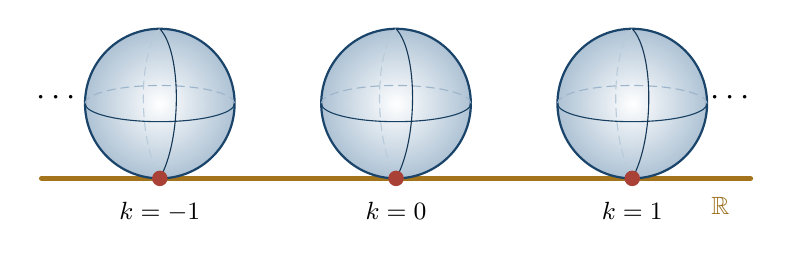
\begin{tikzpicture}[>=Stealth,line cap=round,line join=round]
 \draw[manifoldgold!80!black,line width=2pt]
  (-4.5,0)--(4.5,0);
 \foreach \x/\lab in {-3/{-1},0/{0},3/{1}}{
  \shade[inner color=white,outer color=manifoldblue!37]
   (\x,.95) circle(.95);
  \draw[manifoldblue!75!black,thick]
   (\x,.95) circle(.95);
  \draw[manifoldblue!45,densely dashed,thin]
   ({\x+.95},.95)
   arc[start angle=0,end angle=180,x radius=.95,y radius=.23];
  \draw[manifoldblue!70!black,thin]
   ({\x-.95},.95)
   arc[start angle=180,end angle=360,x radius=.95,y radius=.23];
  \draw[manifoldblue!32,densely dashed,thin]
   (\x,1.9)..controls({\x-.28},1.6)
     and({\x-.28},.5)..(\x,0);
  \draw[manifoldblue!62!black,thin]
   (\x,1.9)..controls({\x+.28},1.6)
     and({\x+.28},.5)..(\x,0);
  \fill[manifoldred] (\x,0) circle(2.8pt);
  \node[below=5pt,font=\small] at (\x,0)
   {$k=\lab$};
 }
 \node[manifoldgold!75!black,font=\small]
  at (4.12,-.35) {$\R$};
 \node[font=\large] at (-4.28,1.02) {$\cdots$};
 \node[font=\large] at (4.28,1.02) {$\cdots$};
\end{tikzpicture}
\caption{Fragment nakrycia uniwersalnego
$S^1\vee S^2$: kopia sfery w każdym
punkcie całkowitym nad pętlą okręgu.
Każda sfera daje inny generator
$\pi_2(X)$, ale wszystkie mają
ten sam obraz w $H_2(X)$.}
\label{fig:nakrycie-bukiet-sfer}
\end{figure}

\begin{uwaga}[Który Whitehead?]
Twierdzenie~\ref{thm:whitehead}
dotyczy słabych równoważności
homotopijnych CW.
\emph{Torsja Whiteheada}
jest innym, późniejszym
niezmiennikiem używanym
przy prostej homotopii
i ogólniejszych
twierdzeniach o
kobordyzmach; sama
nazwa nie czyni jej
częścią tego twierdzenia.
\end{uwaga}

\section*{Dalsza droga}
\addcontentsline{toc}{section}{Dalsza droga}
Następny naturalny blok to
formy różniczkowe,
orientacja, całkowanie,
twierdzenie Stokesa
i kohomologia de Rhama.
Po nich rozwiniemy
geometrię riemannowską:
tensor metryczny, koneksję,
symbole Christoffela,
transport równoległy,
geodezyjne, odwzorowanie
wykładnicze, twierdzenie
Hopfa--Rinowa, krzywiznę
i tensory krzywizny,
pola Jacobiego,
twierdzenia porównawcze
oraz twierdzenie
Gaussa--Bonneta.
\emph{Dopiero po tym bloku}
przejdziemy do teorii
Morse'a, uchwytów,
twierdzenia Smale'a
i chirurgii.
Nie wprowadzamy
tych późniejszych
teorii w obecnym rozdziale.

\section*{Dalsza lektura}
\addcontentsline{toc}{section}{Dalsza lektura}
Allen Hatcher,
\emph{Algebraic Topology},
rozdział 4, §§4.1--4.2,
\url{https://pi.math.cornell.edu/~hatcher/AT/ATch4.pdf},
zawiera pełne rozwinięcie
grup względnych,
przybliżenia komórkowego,
twierdzeń Whiteheada
i Hurewicza.
\clearpage

\chapter{Formy różniczkowe, orientacja i kohomologia de Rhama}
\label{ch:formy-de-rham}
\index{forma rozniczkowa@Forma różniczkowa}

W Rozdziale~\ref{ch:algebra-tensorowa} zbudowaliśmy algebrę
zewnętrzną jednej przestrzeni wektorowej. Teraz wykonamy tę
konstrukcję w każdym punkcie rozmaitości i pozwolimy, by jej
współczynniki zmieniały się gładko. Otrzymamy formy różniczkowe.
Różniczkowanie form, ich całkowanie i twierdzenie Stokesa
połączą rachunek różniczkowy z homologią przestrzeni z
Rozdziału~\ref{ch:homologia-przestrzeni}. Na końcu porównamy
obie teorie kohomologii. Nadal nie potrzebujemy metryki,
koneksji ani krzywizny; tym pojęciom poświęcimy późniejszy blok.

\section{Czym jest forma różniczkowa?}
\label{sec:formy-definicje}

\begin{definicja}[Formy i ich wartości]
\index{formy i ich wartosci@Formy i ich wartości}
\label{def:forma-rozniczkowa}
Niech $M$ będzie gładką rozmaitością wymiaru $n$.
\emph{Formą różniczkową stopnia $k$} na $M$ nazywamy
gładkie pole naprzemiennych form $k$-liniowych:
\[
 \omega_p\in\Lambda^k T_p^*M,
 \qquad \omega\in\Omega^k(M)
 :=\Gamma(\Lambda^k T^*M).
\]
Przy $k=0$ jest to funkcja gładka,
$\Omega^0(M)=C^\infty(M)$; dla $k>n$ otrzymujemy
$\Omega^k(M)=0$. Przyjmujemy też $\Omega^k(M)=0$ dla $k<0$.
Na rozmaitości z brzegiem gładkość
oznacza lokalne przedłużenie współczynników do
otwartego otoczenia w $\R^n$.
\end{definicja}

Forma $1$-stopnia mierzy wektor styczny i zwraca liczbę.
Forma $2$-stopnia mierzy \emph{zorientowane pole} zadane
parą wektorów; zamiana wektorów zmienia znak.
Jeśli $(U,x)$ jest mapą $x=(x^1,\ldots,x^n)$, to
\begin{equation}\label{eq:forma-lokalna}
 \omega|_U=\sum_{i_1<\cdots<i_k}
 a_{i_1\ldots i_k}\,\dd x^{i_1}\wedge\cdots\wedge\dd x^{i_k},
 \qquad a_I\in C^\infty(U).
\end{equation}
Tutaj $\dd x^i|_p(v)=v(x^i)$ jest kowektorem z
Rozdziału~\ref{ch:rozmaitosci}. Jedyność współczynników
wynika z bazy algebry zewnętrznej
(Twierdzenie~\ref{thm:wedge-baza}). Zmiana mapy zmienia
współczynniki, lecz nie samą formę.

\begin{przyklad}[Dwie formy na płaszczyźnie]
Na $\R^2$ forma $\alpha=x\,\dd y-y\,\dd x$
przypisuje wektorowi $(u,v)$ liczbę $xv-yu$.
Forma $\omega=\dd x\wedge\dd y$ spełnia
\[
 \omega((u_1,v_1),(u_2,v_2))
 =u_1v_2-v_1u_2.
\]
Jest to wyznacznik: wartość bezwzględna daje pole
równoległoboku, znak zaś jego orientację.
\end{przyklad}

\begin{figure}[!htbp]
\centering
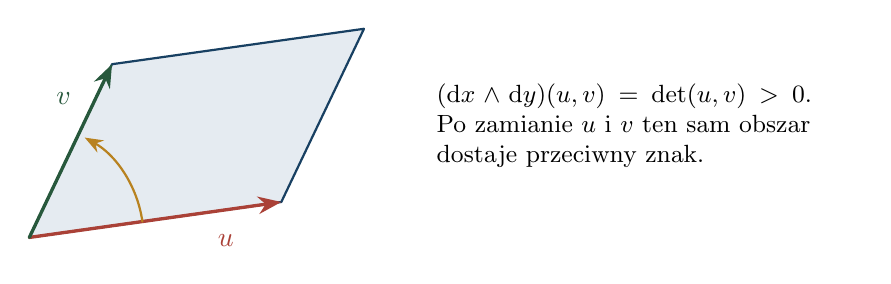
\begin{tikzpicture}[>=Stealth,line cap=round,line join=round]
 \fill[manifoldblue!12] (0,0)--(3.2,.45)--(4.25,2.65)--(1.05,2.2)--cycle;
 \draw[manifoldblue!70!black,thick]
  (0,0)--(3.2,.45)--(4.25,2.65)--(1.05,2.2)--cycle;
 \draw[->,manifoldred,very thick] (0,0)--(3.2,.45)
  node[pos=.78,below=5pt] {$u$};
 \draw[->,manifoldgreen!70!black,very thick] (0,0)--(1.05,2.2)
  node[pos=.8,left=5pt] {$v$};
 \draw[->,manifoldgold!90!black,thick]
  (8:1.45) arc[start angle=8,end angle=61,radius=1.45];
 \node[font=\small,align=left,anchor=west,text width=5.3cm]
  at (5.05,1.42)
  {$(\dd x\wedge\dd y)(u,v)=\det(u,v)>0$.
   Po zamianie $u$ i $v$ ten sam obszar
   dostaje przeciwny znak.};
\end{tikzpicture}
\caption{Forma $\dd x\wedge\dd y$ daje pole ze znakiem
w standardowych współrzędnych płaszczyzny. Ogólna $2$-forma
przypisuje liczbę parze wektorów bez wyboru metryki;
nie musi być euklidesowym polem ich równoległoboku.}
\label{fig:forma-zorientowane-pole}
\end{figure}

\section{Iloczyn zewnętrzny, cofnięcie i różniczka}
\label{sec:formy-dzialania}

\begin{stwierdzenie}[Działania punkt po punkcie]
\label{prop:formy-wedge-pullback}
Dla $\alpha\in\Omega^k(M)$ i $\beta\in\Omega^\ell(M)$
iloczyn $\alpha\wedge\beta\in\Omega^{k+\ell}(M)$
otrzymujemy, biorąc iloczyn zewnętrzny w każdym
$T_p^*M$. Zachodzi $\alpha\wedge\beta
=(-1)^{k\ell}\beta\wedge\alpha$.
Jeżeli $F:M\to N$ jest gładkie, to \emph{cofnięcie}
$F^*:\Omega^k(N)\to\Omega^k(M)$ ma wzór
\begin{equation}\label{eq:pullback-formy}
 (F^*\omega)_p(v_1,\ldots,v_k)
 =\omega_{F(p)}(\dd F_pv_1,\ldots,\dd F_pv_k).
\end{equation}
Spełnia $(G\circ F)^*=F^*G^*$ i
$F^*(\alpha\wedge\beta)=F^*\alpha\wedge F^*\beta$.
\end{stwierdzenie}
\begin{proof}
Gładkość iloczynu w mapie wynika z faktu, że jego
współczynniki są sumami iloczynów gładkich $a_I,b_J$;
przemienność z odpowiednim znakiem jest własnością
algebry zewnętrznej z Rozdziału~\ref{ch:algebra-tensorowa}.
Wzór~\eqref{eq:pullback-formy} jest wieloliniowy i
naprzemienny, a w mapach używa pochodnych współrzędnych
$F$, więc wyznacza formę gładką. Reguła łańcucha
$\dd(G\circ F)_p=\dd G_{F(p)}\circ\dd F_p$
daje własność złożenia. Iloczyn zewnętrzny definiuje
się sumą wartości na przestawionych argumentach; podstawienie
do niej tych samych $\dd F_pv_i$ dowodzi ostatniej równości.
\end{proof}

W szczególności $F^*(\dd y^j)=\dd(y^j\circ F)$.
Jeżeli $F:\R^2\to\R^2$, $F(u,v)=(u^2,v+u)$,
to $F^*(\dd x\wedge\dd y)
=\dd(u^2)\wedge\dd(v+u)=2u\,\dd u\wedge\dd v$.
Współczynnik $2u$ jest wyznacznikiem macierzy Jacobiego
i rejestruje także odwrócenie orientacji przy $u<0$.

\begin{twierdzenie}[Różniczka zewnętrzna]
\label{thm:formy-d}
Istnieje dokładnie jedna rodzina $\R$-liniowych
operatorów $\dd:\Omega^k(M)\to\Omega^{k+1}(M)$
o następujących własnościach:
\begin{enumerate}[leftmargin=*]
\item dla funkcji $f$ forma $\dd f$ jest jej różniczką;
\item $\dd(\alpha\wedge\beta)=\dd\alpha\wedge\beta
 +(-1)^k\alpha\wedge\dd\beta$, gdy $\deg\alpha=k$;
\item $\dd^2=0$.
\end{enumerate}
W mapie jej wzór jest szczególnie prosty:
\begin{equation}\label{eq:zewnetrzna-lokalnie}
 \dd\!\left(\sum_I a_I\,\dd x^I\right)
  =\sum_I\sum_j\frac{\partial a_I}{\partial x^j}
     \dd x^j\wedge\dd x^I,
 \qquad \dd x^I=\dd x^{i_1}\wedge\cdots\wedge\dd x^{i_k}.
\end{equation}
Dla każdego gładkiego $F:M\to N$ zachodzi
$F^*\dd\omega=\dd(F^*\omega)$.
\end{twierdzenie}
\begin{proof}
Najpierw sprawdźmy lokalność dowolnego operatora spełniającego
podane warunki. Jeśli $\omega$ znika w otoczeniu $p$, wybierzmy
gładką funkcję $\chi$, równą $1$ blisko $p$, z nośnikiem
w tym otoczeniu. Taką pojedynczą funkcję buduje się w mapie
z $e^{-1/t}$, jak w dowodzie Twierdzenia
\ref{thm:podzial-jednosci-formy}; nie wymaga to różniczki form.
Ponieważ $\chi\omega=0$, reguła Leibniza daje w $p$
$0=\dd(\chi\omega)_p=(\dd\omega)_p$.
Operator zależy więc tylko od formy w otoczeniu punktu.
Lokalne funkcje i formy możemy pomnożyć przez taką funkcję
odcinającą i przedłużyć przez zero; wynik różniczkowania
blisko $p$ nie zależy od przedłużenia.

Każda forma lokalnie jest sumą wyrazów $a_I\dd x^I$.
Możemy już stosować warunki do lokalnych współrzędnych.
Ponieważ $\dd(\dd x^i)=\dd^2x^i=0$,
reguła Leibniza \emph{wymusza} wzór
\eqref{eq:zewnetrzna-lokalnie}; mamy więc jednoznaczność.
Zdefiniujmy operator tym wzorem. Po powtórnym użyciu
otrzymujemy współczynniki
$(\partial_{x^j}\partial_{x^h}a_I)
\dd x^j\wedge\dd x^h\wedge\dd x^I$.
Wyrazy z $(j,h)$ i $(h,j)$ znoszą się, gdyż pochodne
mieszane są równe, a iloczyn zewnętrzny zmienia znak.
Stąd $\dd^2=0$.

Dla dwóch wyrazów $a\dd x^I$ i $b\dd x^J$
zwykła reguła iloczynu $\dd(ab)=a\dd b+b\dd a$
oraz przestawienie $\dd b$ przez $k$ czynników
$\dd x^I$ dają dokładnie znak $(-1)^k$.
Liniowość rozszerza to na sumy.
Sprawdźmy zgodność na przecięciu map. Cofnięcie przez
zmianę współrzędnych zachowuje $\dd f$ dzięki regule
łańcucha i zachowuje $\wedge$ z poprzedniego
stwierdzenia. Zatem dwa lokalne wzory, obliczone po obu
stronach zmiany współrzędnych, są równe na generatorach
$f,\dd x^i$, a przez regułę Leibniza na wszystkich formach.
Wzory sklejają się w globalny operator. Ten sam argument
dla dowolnego $F$ daje $F^*\dd=\dd F^*$.
\end{proof}

\begin{przyklad}[Rachunek na $\R^3$]
Jeżeli $\alpha=P\,\dd x+Q\,\dd y+R\,\dd z$, to
\[
 \dd\alpha=(Q_x-P_y)\,\dd x\wedge\dd y
 +(R_x-P_z)\,\dd x\wedge\dd z
 +(R_y-Q_z)\,\dd y\wedge\dd z.
\]
Dla $\beta=P\,\dd y\wedge\dd z
+Q\,\dd z\wedge\dd x+R\,\dd x\wedge\dd y$
otrzymujemy $\dd\beta=(P_x+Q_y+R_z)
\dd x\wedge\dd y\wedge\dd z$.
Są to wyrażenia występujące w klasycznych wzorach na rotację
i dywergencję. Utożsamianie tu pól wektorowych z formami
korzysta ze standardowej struktury euklidesowej $\R^3$;
sama różniczka zewnętrzna na $M$ nie wymaga metryki.
\end{przyklad}

\begin{definicja}[Kontrakcja i pochodna Liego]
\index{kontrakcja i pochodna liego@Kontrakcja i pochodna Liego}
\label{def:formy-kontrakcja-lie}
Dla pola wektorowego $X$ operator
$\iota_X:\Omega^k(M)\to\Omega^{k-1}(M)$ określamy przez
\[
 (\iota_X\omega)_p(v_1,\ldots,v_{k-1})
 =\omega_p(X_p,v_1,\ldots,v_{k-1}),
 \qquad \iota_Xf=0.
\]
Jeśli $M$ ma brzeg, w definicji przez dwustronny przepływ
zakładamy, że $X$ jest styczne do $\partial M$.
Jeśli $\Phi_t$ jest lokalnym przepływem $X$ z
Rozdziału~\ref{ch:pola}, kładziemy
$\Lie_X\omega=\left.\frac{\dd}{\dd t}\right|_{t=0}\Phi_t^*\omega$.
\end{definicja}

\begin{twierdzenie}[Wzór Cartana]
\label{thm:cartan-formy}
Dla każdej formy $\omega$ mamy
\begin{equation}\label{eq:cartan-formula}
 \boxed{\ \Lie_X\omega=\dd(\iota_X\omega)
       +\iota_X(\dd\omega)\ }.
\end{equation}
Ponadto $\Lie_X\dd=\dd\Lie_X$ oraz
$\iota_X(\alpha\wedge\beta)=
(\iota_X\alpha)\wedge\beta
+(-1)^{\deg\alpha}\alpha\wedge\iota_X\beta$.
\end{twierdzenie}
Dla pola niestycznego do brzegu prawa strona wzoru Cartana
nadal określa gładką formę. Możemy nią zdefiniować
$\Lie_X\omega$ na brzegu: jest to przedłużenie pochodnej
Liego z wnętrza, niezależne od przedłużeń w mapach.
Nie zakładamy wówczas istnienia dwustronnego przepływu w $M$.
\begin{proof}
Ostatnia równość wynika wprost z definicji iloczynu
zewnętrznego: po wstawieniu $X$ w pierwsze miejsce
może on wejść do pierwszej grupy argumentów lub,
po przejściu przez $\deg\alpha$ argumentów, do drugiej.
Ponieważ $\Phi_t^*$ zachowuje iloczyn zewnętrzny,
$\Lie_X$ jest derywacją stopnia $0$ algebry form.
Prawa strona~\eqref{eq:cartan-formula} również nią jest:
rozwijamy oba składniki na $\alpha\wedge\beta$
regułami dla $\dd$ i $\iota_X$; wyrazy mieszane mają
przeciwne znaki i znoszą się.

Wystarczy zatem porównać obie strony na lokalnych
generatorach $f,\dd x^i$. Dla funkcji lewa strona to
$Xf$, a prawa to $\iota_X\dd f=\dd f(X)=Xf$.
Dla $\dd x^i$ lewa strona wynosi
$\dd(\Lie_Xx^i)=\dd(Xx^i)$, gdyż cofnięcie
komutuje z $\dd$; prawa wynosi
$\dd(\iota_X\dd x^i)+\iota_X\dd^2x^i
=\dd(Xx^i)$. Wzór obowiązuje więc dla
każdej sumy wyrazów $f\,\dd x^I$ i globalnie.
Wreszcie, z $\dd^2=0$ dostajemy
$\dd\Lie_X=\dd\iota_X\dd
=\Lie_X\dd$.
\end{proof}

\begin{przyklad}[Pochodna Liego formy]
Na $\R^2$ weźmy $X=\partial_x$ i $\omega=x\,\dd y$.
Przepływ przesuwa punkty poziomo, więc
$\Phi_t^*\omega=(x+t)\dd y$ oraz
$\Lie_X\omega=\dd y$. Ze wzoru Cartana:
$\iota_X\omega=0$, $\dd\omega=\dd x\wedge\dd y$
i $\iota_X\dd\omega=\dd y$. Oba obliczenia są zgodne.
\end{przyklad}
\section{Lokalne istnienie funkcji pierwotnej}
\label{sec:formy-poincare}

Równość $\dd^2=0$ mówi, że każda forma postaci
$\dd\eta$ jest \emph{zamknięta}. Odwrotność nie zachodzi
globalnie: przeszkodę może stanowić topologia. Lokalnie
przeszkoda znika, co wyjaśnia następujący rachunek.
Dla zamkniętej $1$-formy $\omega$ szukamy \emph{funkcji
pierwotnej} $f$ spełniającej $\omega=\dd f$.
Dla formy stopnia $k>1$ jej odpowiednikiem jest
\emph{forma pierwotna} $\eta$ stopnia $k-1$ z
$\omega=\dd\eta$. Lemat Poincarégo obejmuje
oba przypadki.

\begin{lemat}[Homotopia form]
\label{lem:homotopia-form}
Niech $H:[0,1]\times M\to N$ będzie gładką homotopią
odwzorowań $H_0,H_1$. Przy końcach przedziału, a także
przy narożach iloczynu, gdy $M$ ma brzeg, gładkość
rozumiemy jako gładkie przedłużanie składowych w mapach. Istnieje operator liniowy
$K:\Omega^k(N)\to\Omega^{k-1}(M)$ taki, że
\begin{equation}\label{eq:homotopia-form}
 H_1^*\omega-H_0^*\omega
 =\dd(K\omega)+K(\dd\omega).
\end{equation}
\end{lemat}
\begin{proof}
Dla $k=0$ przyjmujemy $K\omega=0$; poniższy rachunek
obejmuje ten przypadek z $a=0$. Każdą formę na
$[0,1]\times M$ zapisujemy jednoznacznie
w postaci $H^*\omega=\dd t\wedge a(t)+b(t)$,
gdzie $a(t)$ jest rodziną form stopnia $k-1$ na $M$,
a $b(t)$ rodziną form stopnia $k$. Położenie
$K\omega:=\int_0^1 a(t)\,\dd t$ oznacza całkowanie
\emph{współczynników} formy po parametrze; można je
wykonać w każdej mapie, a zgodność na przecięciach
wynika z liniowości zmiany współrzędnych.
Obliczenie różniczki daje
\[
 \dd(H^*\omega)
 =\dd t\wedge(\partial_tb-\dd_Ma)+\dd_Mb.
\]
Ponieważ $H^*\dd\omega=\dd H^*\omega$, współczynniki
przy $\dd t$ mówią, że
$a_{\dd\omega}(t)=\partial_tb(t)-\dd_Ma(t)$.
Po scałkowaniu od $0$ do $1$ otrzymujemy
$K\dd\omega=b(1)-b(0)-\dd_MK\omega$.
Ale $b(i)=H_i^*\omega$ dla $i=0,1$,
więc jest to dokładnie~\eqref{eq:homotopia-form}.
\end{proof}

\begin{twierdzenie}[Lemat Poincarégo]
\label{thm:lemat-poincare-formy}
Niech $U\subset\R^n$ będzie otwarty i gwiaździsty
względem $0$. Jeżeli $k\geq1$ i
$\omega\in\Omega^k(U)$ spełnia $\dd\omega=0$,
to istnieje $\eta\in\Omega^{k-1}(U)$ z
$\omega=\dd\eta$. Każda zamknięta forma stopnia
$0$ jest stała na $U$.
\end{twierdzenie}
\begin{proof}
W Lemacie~\ref{lem:homotopia-form} bierzemy
$H(t,x)=tx$. Dla $k\geq1$ odwzorowanie $H_0$
jest stałe, więc $H_0^*\omega=0$; dla zamkniętej
$\omega$ drugi składnik po prawej stronie
\eqref{eq:homotopia-form} także znika.
Dostajemy $\omega=\dd(K\omega)$.
Jeśli chcemy \emph{obliczyć} formę pierwotną
(dla $k=1$: funkcję pierwotną), to
\begin{equation}\label{eq:poincare-pierwotna}
 (K\omega)_x(v_1,\ldots,v_{k-1})
 =\int_0^1 t^{k-1}
   \omega_{tx}(x,v_1,\ldots,v_{k-1})\,\dd t.
\end{equation}
Istotnie, $\dd H(\partial_t)=x$, podczas gdy
$\dd H(v_i)=tv_i$, skąd $k-1$ czynników $t$.
Gwiaździstość zapewnia, że cały odcinek $tx$ leży w $U$.
Dla $k=0$ warunek $\dd f=0$ mówi, że wszystkie
pochodne kierunkowe znikają. Zatem pochodna
$t\mapsto f(tx)$ jest zerowa i $f(x)=f(0)$.
\end{proof}

\begin{przyklad}[Obliczenie funkcji pierwotnej]
Na $\R^2$ forma $\omega=2xy\,\dd x+x^2\,\dd y$
jest zamknięta, bo
$\dd\omega=(2x-2x)\dd x\wedge\dd y=0$.
Wzór~\eqref{eq:poincare-pierwotna} dla $k=1$ daje
\[
 (K\omega)(x,y)=\int_0^1
 \omega_{(tx,ty)}(x,y)\,\dd t
 =\int_0^1 3t^2x^2y\,\dd t=x^2y.
\]
Zatem $f(x,y)=x^2y$ jest funkcją pierwotną
$1$-formy $\omega$, ponieważ $\omega=\dd f$.
Obliczenie pokazuje mechanizm lematu.
\end{przyklad}

\begin{wniosek}[Niezmienniczość przez homotopię]
\label{cor:de-rham-homotopia}
Odwzorowania gładko homotopijne indukują tę samą
operację cofnięcia na kohomologii de Rhama
z Definicji~\ref{def:de-rham-cohomology}.
\end{wniosek}
\begin{proof}
Jeśli $\dd\omega=0$, wzór~\eqref{eq:homotopia-form}
mówi, że $H_1^*\omega-H_0^*\omega=\dd(K\omega)$.
Różnica jest więc dokładna i obie klasy są równe.
\end{proof}

\section{Podział jedności}
\label{sec:formy-podzial-jednosci}

Przy całkowaniu trzeba scalać dane z wielu map.
Służy do tego wynik, który wyjaśnia także wcześniejsze
użycia funkcji odcinających w skrypcie.

\begin{twierdzenie}[Gładki podział jedności]
\label{thm:podzial-jednosci-formy}
Niech $(U_\alpha)$ będzie otwartym pokryciem rozmaitości
$M$ Hausdorffa i o przeliczalnej bazie. Istnieją
nieujemne funkcje gładkie $(\rho_j)$ o lokalnie skończonej
rodzinie nośników (każdy punkt ma otoczenie spotykające
tylko skończenie wiele nośników) oraz indeksy $\alpha(j)$ takie, że
\[
 \supp\rho_j\subset U_{\alpha(j)},
 \qquad \sum_j\rho_j(p)=1\quad(p\in M).
\]
Każdą $\rho_j$ można wybrać o nośniku zwartym
w jednej dziedzinie mapy zawartej w $U_{\alpha(j)}$.
\end{twierdzenie}
\begin{proof}
Najpierw budujemy jedną funkcję odcinającą.
Jeśli w mapie kula domknięta $\overline B_r$
leży w większej kuli $B_R$, przy czym $0<r<R$
i $\overline B_R$ zawiera się w obrazie mapy,
wybierzmy gładką funkcję $\chi$ zależną tylko
od $\|x\|^2$, równą $1$ na $\overline B_r$,
dodatnią między $r$ i $R$, a zerową poza $B_R$.
Można ją złożyć z funkcji $h(t)=e^{-1/t}$ dla
$t>0$ i $h(t)=0$ dla $t\leq0$; jej gładkość w
$t=0$ wynika z zanikania wszystkich pochodnych
$t^{-a}e^{-1/t}$. Przedłużenie $\chi$ przez $0$
na resztę $M$ jest gładkie, bo nośnik ma zwartą
domkniętą otoczkę wewnątrz mapy. Przy brzegu bierzemy
przecięcia tych kul z półprzestrzenią i ograniczamy do nich
te same funkcje. Wszystkie wnętrza i domknięcia poniżej
rozumiemy w topologii $M$, także przy brzegu.

Z lokalnej zwartości i przeliczalności bazy
konstruujemy wyczerpanie zwartymi zbiorami
$K_1\subset\operatorname{int}K_2\subset\cdots$,
$\bigcup_jK_j=M$ (weźmy kolejno skończone
sumy domkniętych, stosunkowo zwartych kul
obejmujące pierwsze elementy przeliczalnego
pokrycia i powiększmy je przy każdym kroku).
Ustalmy $K_j=\varnothing$ dla $j\leq0$.
Zwarty pas $K_j\setminus\operatorname{int}K_{j-1}$
można pokryć skończenie wieloma małymi kulami
w mapach o domknięciach zawartych jednocześnie
w którymś $U_\alpha$ i w
$\operatorname{int}K_{j+1}\setminus K_{j-2}$.
Wybieramy funkcje odcinające dodatnie na
mniejszych kulach pokrywających pas.
Rodzina tych kul dla wszystkich $j$ jest
lokalnie skończona: otoczenie punktu wewnątrz
pewnego $K_N$ nie spotyka kul pochodzących
z pasów o dostatecznie dużym indeksie.

Niech $\chi_j$ oznaczają wszystkie otrzymane
funkcje. Suma $S=\sum_j\chi_j$ jest lokalnie
skończona, gładka i wszędzie dodatnia, bo
każdy punkt należy do któregoś pasa. Kładziemy
$\rho_j=\chi_j/S$. Wtedy nośniki pozostają
w wybranych kulach i
$\sum_j\rho_j=S/S=1$.
Gdy potrzebujemy funkcji indeksowanych samymi zbiorami
pokrycia, sumujemy $\rho_j$ o tym samym $\alpha(j)$.
Nośnik takiej sumy nadal leży w $U_\alpha$:
lokalnie skończona suma zamkniętych nośników jest
zbiorem domkniętym zawartym w $U_\alpha$.
\end{proof}
\section{Orientowalność i orientacje indukowane}
\label{sec:formy-orientacja}

\begin{definicja}[Orientacja]
\index{orientacja@Orientacja}
\label{def:orientacja-formy}
Dwie uporządkowane bazy $m$-wymiarowej przestrzeni
rzeczywistej $V$, dla $m\geq1$, mają tę samą orientację, jeśli
macierz przejścia ma dodatni wyznacznik.
Powstają dwie klasy baz. Na rozmaitości $M^m$
\emph{orientacja} to gładki wybór takiej klasy w
każdym $T_pM$. Równoważnie jest to klasa
nigdzie niezerowych form $m$-stopnia: formy
$\mu,\nu$ wyznaczają tę samą orientację, jeśli
$\nu=f\mu$ dla gładkiej funkcji $f>0$.
Rozmaitość dopuszczająca taki wybór jest
\emph{orientowalna}; wraz z wyborem orientacji
jest \emph{zorientowana}.
\end{definicja}

W wymiarze $0$ stosujemy opis przez formy najwyższego
stopnia: $\Lambda^0 V^*=\R$, a orientacja jest wyborem
jednej z dwóch półprostych, czyli znaku $+1$ lub $-1$.
Każdemu punktowi rozmaitości dyskretnej przypisujemy taki
znak. Opis przez dwie klasy baz dotyczy tylko $m\geq1$,
gdyż przestrzeń zerowa ma tylko jedną bazę pustą.

Dla $m\geq1$ forma $\mu_p$ określa bazę dodatnią $(v_1,\ldots,v_m)$
przez nierówność $\mu_p(v_1,\ldots,v_m)>0$.
To definicja \emph{znaku}, a nie długości ani pola:
zamiana $\mu$ na $2\mu$ nie zmienia orientacji.
Na każdej spójnej orientowalnej rozmaitości istnieją
dwa wybory globalne, wzajemnie przeciwne.

\begin{twierdzenie}[Trzy opisy orientowalności]
\label{thm:orientacja-atlas-forma}
Dla rozmaitości gładkiej $M^m$ równoważne są
poniższe warunki. W mapach przy brzegu dopuszczamy
obie półprzestrzenie $x^m\geq0$ i $x^m\leq0$;
jest to ta sama struktura gładka, a pozwala stosować
odbicie współrzędnej także w wymiarze $1$.
\begin{enumerate}[leftmargin=*]
\item orientowalność $M$;
\item istnienie atlasu, w którym wszystkie wyznaczniki
      odwzorowań przejścia są dodatnie;
\item istnienie globalnej nigdzie niezerowej formy
      $\mu\in\Omega^m(M)$.
\end{enumerate}
\end{twierdzenie}
\begin{proof}
Dla $m=0$ wszystkie trzy warunki są spełnione:
rozmaitość jest dyskretna, dowolny wybór znaków jest
gładki, a funkcja $1$ jest nigdzie niezerową $0$-formą.
Atlas zerowymiarowy sam nie zapisuje wyboru znaków.
Załóżmy więc $m\geq1$.
Forma $\mu$ wybiera dodatnie bazy w każdym punkcie,
więc (3) daje (1). Jeśli wybór (1) jest ustalony,
zmniejszamy dziedziny map do spójnych otoczeń.
Każdą mapę można w razie potrzeby złożyć z odbiciem
jednej współrzędnej, aby jej standardowa baza była
dodatnia. W nowym atlasie dwie bazy lokalne opisują
tę samą orientację, zatem ich wyznacznik przejścia
jest dodatni: (1) daje (2).

Załóżmy (2). W każdej mapie z tego atlasu lokalna
forma $\mu_j=\dd x_j^1\wedge\cdots\wedge\dd x_j^m$
jest dodatnia. Wybierzmy podział jedności $(\rho_j)$
z Twierdzenia~\ref{thm:podzial-jednosci-formy},
o nośnikach w dziedzinach tych map, i przedłużmy
$\rho_j\mu_j$ przez zero. Suma
$\mu=\sum_j\rho_j\mu_j$ jest lokalnie skończona.
W dowolnym punkcie co najmniej jedno $\rho_j$ jest
dodatnie; wszystkie występujące $\mu_j$ są dodatnimi
wielokrotnościami jednej z nich, bo przejścia
mają dodatni wyznacznik. Suma nie może się
wyzerować. Tak dostajemy (3).
\end{proof}

\begin{stwierdzenie}[Dwa podstawowe sposoby przenoszenia orientacji]
\label{prop:orientacja-iloczyn-pullback}
Jeżeli $F:M\to N$ jest dyfeomorfizmem i $N$ ma
orientację $[\nu]$, to $F^*\nu$ orientuje $M$;
$F$ zachowuje orientację wtedy, gdy zgadza się ona
z uprzednio wybraną orientacją $M$. Jeśli $M^m,N^n$
są zorientowane, orientację $M\times N$ wyznacza
$\pr_M^*\mu\wedge\pr_N^*\nu$.
Po zamianie kolejności czynników znak zmienia się
o $(-1)^{mn}$.
\end{stwierdzenie}
\begin{proof}
Różniczka dyfeomorfizmu jest izomorfizmem, więc
cofnięcie nigdzie niezerowej formy najwyższego stopnia
pozostaje nigdzie niezerowe. Na iloczynie wartości
$\mu\wedge\nu$ na bazie najpierw $TM$, potem $TN$
są dodatnie. Przestawienie $m$ wektorów z pierwszego
czynnika z $n$ wektorami drugiego wymaga $mn$
zamian; każda zmienia znak formy.
\end{proof}

Orientacja brzegu i orientacja regularnego zbioru
poziomicowego są dwiema wersjami tej samej zasady:
\emph{najpierw kierunki normalne, potem styczne}.

\begin{definicja}[Orientacja brzegu: normalna na zewnątrz]
\index{orientacja brzegu normalna na zewnatrz@Orientacja brzegu: normalna na zewnątrz}
\label{def:orientacja-brzegu}
Niech $M^m$ będzie zorientowaną rozmaitością z brzegiem.
Dla $m\geq2$ baza $(v_1,\ldots,v_{m-1})$ przestrzeni $T_p\partial M$
jest dodatnia wtedy i tylko wtedy, gdy
$(n,v_1,\ldots,v_{m-1})$ jest dodatnią bazą $T_pM$
dla dowolnego wektora $n$ skierowanego na zewnątrz.
Wymóg nie zależy od konkretnego $n$: dwa takie wektory
mają dodatnio proporcjonalne składowe poprzeczne,
a dodanie wektora stycznego nie zmienia wyznacznika.
Równoważnie, dla formy $\mu$ reprezentującej orientację,
brzeg orientuje $\iota_n\mu$ ograniczona do $T\partial M$.
Ten opis działa również dla $m=1$: znak w punkcie brzegu
jest znakiem liczby $\mu_p(n)$.
\end{definicja}

\begin{stwierdzenie}[Brzeg jest orientowalny]
\label{prop:brzeg-orientowalny}
Powyższa reguła nadaje $\partial M$ gładką orientację.
Dla standardowej orientacji $[a,b]$ końcowy punkt $b$
ma znak $+1$, a początkowy $a$ ma znak $-1$.
Dla dysku $D^2$ ze standardową orientacją płaszczyzny
brzeg biegnie przeciwnie do ruchu wskazówek zegara.
\end{stwierdzenie}
\begin{proof}
W mapie półprzestrzeni $\{x^m\geq0\}$ kierunek
na zewnątrz to $-\partial_{x^m}$; reguła daje
stały wybór znaku baz współrzędnych stycznych.
Zmiany map zachowują orientację $M$ i wysyłają
kierunek na zewnątrz na kierunek na zewnątrz,
więc uzyskane wybory na przecięciach są zgodne.
W wymiarze $1$ przy $b$ wektor zewnętrzny
$+\partial_t$ jest dodatni, a przy $a$ wektor
$-\partial_t$ ujemny. W dysku przy $(1,0)$
wektor zewnętrzny jest $(1,0)$; aby para była
dodatnia, wektor styczny musi wskazywać $(0,1)$.
Ciągłość przenosi ten kierunek na cały okrąg.
\end{proof}

\begin{figure}[!htbp]
\centering
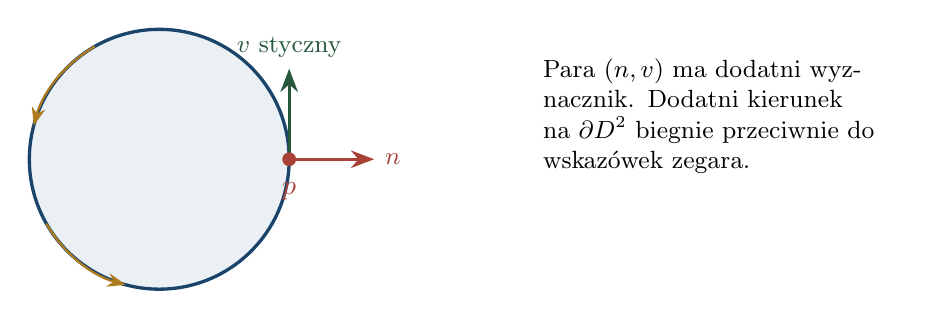
\begin{tikzpicture}[>=Stealth,line cap=round,line join=round]
 \fill[manifoldblue!9] (0,0) circle (1.65);
 \draw[manifoldblue!75!black,line width=1.2pt] (0,0) circle (1.65);
 \draw[->,manifoldred,very thick] (1.65,0)--(2.73,0)
  node[right,font=\small] {$n$};
 \draw[->,manifoldgreen!70!black,very thick] (1.65,0)--(1.65,1.15)
  node[above,font=\small] {$v$ styczny};
 \draw[->,manifoldgold!85!black,thick]
  (210:1.65) arc[start angle=210,end angle=255,radius=1.65];
 \draw[->,manifoldgold!85!black,thick]
  (120:1.65) arc[start angle=120,end angle=165,radius=1.65];
 \fill[manifoldred] (1.65,0) circle(2.5pt)
  node[below=5pt] {$p$};
 \node[font=\small,align=left,anchor=west,text width=4.6cm]
  at (4.75,.55)
  {Para $(n,v)$ ma dodatni wyznacznik.
   Dodatni kierunek na $\partial D^2$
   biegnie przeciwnie do wskazówek zegara.};
\end{tikzpicture}
\caption{Orientację brzegu wyznacza reguła
„normalna na zewnątrz jako pierwszy wektor”.}
\label{fig:orientacja-brzegu-dysk}
\end{figure}

\begin{twierdzenie}[Orientacja regularnego przeciwobrazu]
\label{thm:orientacja-poziomicy}
Niech $F:M^m\to N^q$ będzie gładkie,
$M,N$ zorientowane, $N$ bez brzegu, a $y\in N$ wartością
regularną. Jeśli $M$ ma brzeg, zakładamy ponadto, że $y$
jest wartością regularną $F|_{\partial M}$.
Wtedy $S=F^{-1}(y)$ jest orientowalną podrozmaitością
wymiaru $m-q$ (o ile nie jest pusta). Orientację
można określić dla wszystkich wymiarów następująco.
Dla dodatnich form objętości $\mu_p$ na $T_pM$
i $\nu_y$ na $T_yN$, dowolnej bazy $(e_1,\ldots,e_q)$
oraz podniesień $\dd F_pw_i=e_i$ kładziemy
\[
 \eta_p(v_1,\ldots,v_{m-q})
 =\frac{\mu_p(w_1,\ldots,w_q,v_1,\ldots,v_{m-q})}
        {\nu_y(e_1,\ldots,e_q)}.
\]
Puste listy argumentów oznaczają wartości form stopnia $0$.
Forma $\eta$ określa orientację $S$. Gdy $q\geq1$
i $m-q\geq1$, jest to reguła: $(v_1,\ldots,v_{m-q})$
w $T_pS=\ker\dd F_p$ jest dodatnia, jeśli dla
wektorów $w_1,\ldots,w_q\in T_pM$, których obrazy
$(\dd F_pw_1,\ldots,\dd F_pw_q)$ tworzą dodatnią
bazę $T_yN$, ciąg
$(w_1,\ldots,w_q,v_1,\ldots,v_{m-q})$
jest dodatni w $T_pM$. Gdy $m=q$, punktowi $p\in S$
przypisujemy znak izomorfizmu $\dd F_p$ między
zorientowanymi przestrzeniami. Przy brzegu
$\partial S=S\cap\partial M$.
\end{twierdzenie}
\begin{proof}
Regularność znaczy, że $\dd F_p$ jest surjekcją,
więc takie $w_i$ istnieją. Przy $\partial M$ dodatkowa
surjekcja na przestrzeni stycznej do brzegu pozwala wybrać
$q$ współrzędnych stycznych, w których pochodne $F$ są
niezależne. Twierdzenie o funkcji odwrotnej zastosowane
do $F$ wraz z pozostałymi współrzędnymi, w tym współrzędną
normalną $s\geq0$, daje lokalną postać poziomicy
$\R^{m-q-1}\times[0,\infty)$. Stąd podana formuła brzegu.
Bez założenia o $F|_{\partial M}$ wniosek mógłby zawieść:
dla $F(x,s)=x^2+s$ na $s\geq0$ wartość $0$ jest regularna
dla $F$, lecz przeciwobraz jest pojedynczym punktem,
a nie oczekiwaną jednowymiarową podrozmaitością z brzegiem. Zastąpienie $w_i$
innymi podniesieniami zmienia je o elementy
$\ker\dd F_p$; macierz zmiany bazy ma wówczas
blok trójkątny z jednostką na przekątnej w części
normalnej, zatem nie zmienia znaku. Zmiana
dodatniej bazy w $T_yN$ ma dodatni wyznacznik
i także zachowuje znak. Reguła jest więc
jednoznaczna. W ilorazowym wzorze na $\eta_p$ zmiana
dowolnej bazy $(e_i)$ mnoży licznik i mianownik przez
ten sam niezerowy wyznacznik; zmiana dodatnich form
$\mu_p,\nu_y$ mnoży wynik przez liczbę dodatnią.
W lokalnej postaci submersji z
Wniosku~\ref{wn:submersja-lokalnie} wybory normalnych
i stycznych są gładkie; znaki są zgodne na przecięciach.
To dowodzi orientowalności $S$ i wzoru.
\end{proof}

Ta konstrukcja działa też dla zorientowanej
\emph{wiązki normalnej} podrozmaitości $S\subset M$:
jej baza dodatnia, a następnie baza $TS$ mają razem
dawać bazę dodatnią $TM$. Wybór orientacji normalnej
nazywamy \emph{koorientacją}. Bez takiego wyboru sama
orientacja $M$ nie zawsze orientuje $S$.

\begin{przyklad}[Okrąg jako poziomica]
W $\R^2$ i $\R$ wybierzmy orientacje standardowe
i weźmy $F(x,y)=x^2+y^2$. Na $S^1=F^{-1}(1)$
różniczka ma wartość dodatnią na wektorze
skierowanym promieniowo na zewnątrz.
Twierdzenie~\ref{thm:orientacja-poziomicy} daje więc
orientację przeciwną do ruchu wskazówek zegara,
taką samą jak orientacja brzegu $D^2$.
\end{przyklad}

\begin{przyklad}[Co zawodzi na wstędze i przestrzeni rzutowej]
Wstęga Möbiusa z Przykładu~\ref{prz:mobius}
po jednym okrążeniu odwraca
kierunek poprzeczny, zachowując kierunek
wzdłuż okręgu. Orientacja płaszczyzny stycznej
musiałaby więc zmienić znak i nie może być globalna.
Jej brzeg jest jednak okręgiem, a zatem orientowalnym.

Dla $n\geq1$ przestrzeń $\mathbb{RP}^n$ jest
orientowalna dokładnie wtedy, gdy $n$ jest nieparzyste.
Istotnie, nakrycie $S^n\to\mathbb{RP}^n$ identyfikuje
$x$ z $-x$. Antypodalne $A(x)=-x$ zmienia orientację
$S^n$ o znak $(-1)^{n+1}$: dodatnią bazę przestrzeni otaczającej
otrzymujemy z $(x,v_1,\ldots,v_n)$ w $\R^{n+1}$,
a $A$ mnoży wszystkie $n+1$ wektorów przez $-1$.
Orientacja na ilorazie istnieje wtedy i tylko wtedy,
gdy to utożsamienie zachowuje orientację sfery:
jeśli zachowuje, orientacja schodzi przez lokalne
dyfeomorfizmy; jeśli odwraca, jej podniesienie z
ilorazu byłoby zarazem zachowane i odwrócone, co
jest niemożliwe na spójnej sferze.
\end{przyklad}
\section{Całkowanie form na rozmaitości}
\label{sec:formy-calkowanie}

Na zorientowanej rozmaitości $M^m$ całkujemy formy
stopnia $m$: mają dokładnie tyle argumentów, ile
niezależnych kierunków ma $M$. Bez orientacji można
całkować \emph{gęstości}, ale wymagają osobnej definicji;
całka z formy najwyższego stopnia potrzebuje znaku.

\begin{definicja}[Całka z formy o zwartym nośniku]
\index{calka z formy o zwartym nosniku@Całka z formy o zwartym nośniku}
\label{def:calka-z-formy}
Niech $M^m$ będzie zorientowana i
$\omega\in\Omega_c^m(M)$, gdzie dolny indeks $c$
oznacza zwarty nośnik. W mapie $(U,x)$ zgodnej z
orientacją, jeśli $\supp\omega\subset U$ i
$\omega=f\,\dd x^1\wedge\cdots\wedge\dd x^m$,
definiujemy
\begin{equation}\label{eq:calka-lokalna}
 \int_M\omega:=\int_{x(U)} f(x^{-1}(u))\,\dd u^1\cdots\dd u^m.
\end{equation}
Dla dowolnego zwartego nośnika bierzemy podział
jedności $(\rho_j)$ z Twierdzenia
\ref{thm:podzial-jednosci-formy}, w mapach zgodnych
z orientacją, i kładziemy
\begin{equation}\label{eq:calka-globalna}
 \int_M\omega:=\sum_j\int_M\rho_j\omega.
\end{equation}
Tylko skończenie wiele składników może być niezerowych:
lokalnie skończona rodzina nośników spotyka zwarty
$\supp\omega$ tylko dla skończenie wielu indeksów.
W wymiarze $0$ definicję zastępuje suma
$\int_M f=\sum_{p\in M}\varepsilon_p f(p)$,
gdzie $\varepsilon_p\in\{1,-1\}$ jest orientacją punktu.
Zwarty nośnik w przestrzeni dyskretnej jest skończony.
\end{definicja}

\begin{twierdzenie}[Niezależność od map i podziału]
\label{thm:calka-dobrze-okreslona}
Definicja~\ref{def:calka-z-formy} nie zależy od
wybranego dodatniego atlasu ani podziału jedności.
Jeżeli $F:M\to N$ jest dyfeomorfizmem zachowującym
orientację, to dla $\omega\in\Omega_c^m(N)$ zachodzi
$\int_M F^*\omega=\int_N\omega$; gdy $F$ odwraca
orientację i $M,N$ są spójne, po prawej pojawia się
znak minus.
\end{twierdzenie}
\begin{proof}
W wymiarze $0$ teza wynika z sumy ze znakami i z tego,
że dyfeomorfizm jest bijekcją punktów. Dla $m\geq1$
najpierw niech nośnik leży w dwóch dodatnich mapach
$x$ i $y$. Z równości
\[
 \dd y^1\wedge\cdots\wedge\dd y^m
 =\det D(y\circ x^{-1})\,
   \dd x^1\wedge\cdots\wedge\dd x^m
\]
wynika, że współczynniki opisujące tę samą formę
w obu mapach różnią się o wyznacznik Jacobiego.
Jest on dodatni. Twierdzenie o zmianie zmiennych
w całce na otwartych podzbiorach $\R^m$ pokazuje,
że oba wzory~\eqref{eq:calka-lokalna} dają tę samą
liczbę. Dla mapy odwracającej orientację wyznacznik
jest ujemny, a zwykły wzór na zmianę zmiennych
zawiera jego wartość bezwzględną; stąd minus.

Jeśli $(\rho_j)$ i $(\sigma_k)$ są dwoma podziałami,
to na nośniku $\omega$ możemy wstawić
$1=\sum_k\sigma_k$ do każdej całki $\rho_j\omega$.
Otrzymujemy sumę $\sum_{j,k}\int_M\rho_j\sigma_k\omega$.
Każdy składnik ma nośnik w przecięciu dwóch map.
Rozcinamy go w razie potrzeby na mniejsze mapy,
stosujemy poprzedni rachunek i zamieniamy kolejność
obu skończonych sum. Wynik jest taki sam, gdy
zaczniemy od $(\sigma_k)$. Wzór dla $F$ sprawdzamy
na składnikach lokalnych przez $y\circ F\circ x^{-1}$
i sumujemy.
\end{proof}

Na zwartej rozmaitości każda gładka forma ma zwarty
nośnik. Dla zorientowanej krzywej parametryzowanej
$\gamma:[a,b]\to M$ całka z $1$-formy jest
$\int_\gamma\alpha:=\int_a^b\gamma^*\alpha$;
przeparametryzowanie zachowujące kierunek nie zmienia
jej wartości. Dla parametryzowanej powierzchni
analogicznie cofamy formę $2$-stopnia.

\begin{przyklad}[Całka po okręgu]
Dla $\gamma(t)=(\cos t,\sin t)$, $0\leq t\leq2\pi$,
zorientowanej przeciwnie do ruchu wskazówek zegara,
forma $\alpha=x\,\dd y-y\,\dd x$ daje
$\gamma^*\alpha=(\cos^2t+\sin^2t)\dd t=\dd t$.
Stąd $\int_{S^1}\alpha=2\pi$.
Nie jest to długość łuku wyprowadzona z metryki:
całkujemy $1$-formę wybraną w otaczającej płaszczyźnie.
\end{przyklad}

\section{Twierdzenie Stokesa}
\label{sec:formy-stokes}

Intuicja jest jedna: gdy zsumujemy brzegi
małych, zgodnie zorientowanych fragmentów,
ich wewnętrzne krawędzie wystąpią po dwa razy
z przeciwnymi znakami. Pozostanie brzeg całości.
Rachunek na formach pozwala zapisać tę zasadę
bez ograniczania się do konkretnych wymiarów.

\begin{figure}[!htbp]
\centering
\begin{tikzpicture}[>=Stealth,line cap=round,line join=round]
 \fill[manifoldblue!10] (0,0) rectangle (3,2.35);
 \fill[manifoldgreen!12] (3,0) rectangle (6,2.35);
 \draw[manifoldblue!70!black,thick] (0,0) rectangle (3,2.35);
 \draw[manifoldgreen!70!black,thick] (3,0) rectangle (6,2.35);
 \draw[->,manifoldred,very thick] (2.92,.6)--(2.92,1.68);
 \draw[->,manifoldgold!85!black,very thick] (3.08,1.68)--(3.08,.6);
 \draw[->,manifoldblue!70!black,thick] (.65,0)--(1.75,0);
 \draw[->,manifoldgreen!70!black,thick] (4.25,0)--(5.35,0);
 \node[manifoldblue!80!black] at (1.5,1.25) {$P_1$};
 \node[manifoldgreen!70!black] at (4.5,1.25) {$P_2$};
 \node[font=\small,align=left,anchor=west,text width=5.0cm]
  at (6.55,1.2)
  {Wspólna krawędź jest brzegiem $P_1$
   i $P_2$ z przeciwnymi kierunkami.
   W sumie znika; zostaje tylko brzeg zewnętrzny.};
\end{tikzpicture}
\caption{Znak orientacji usuwa wewnętrzną krawędź
przy składaniu dwóch fragmentów.}
\label{fig:stokes-anulowanie}
\end{figure}

\begin{twierdzenie}[Stokes dla form]
\label{thm:stokes-formy}
Niech $M^m$ będzie zorientowaną gładką rozmaitością
z brzegiem, $m\geq1$, a $\omega\in\Omega_c^{m-1}(M)$.
Brzeg ma orientację z Definicji
\ref{def:orientacja-brzegu}, a
$i:\partial M\hookrightarrow M$ jest \emph{inkluzją}.
Wtedy
\begin{equation}\label{eq:stokes-formy}
 \boxed{\displaystyle \int_M\dd\omega
        =\int_{\partial M}i^*\omega.}
\end{equation}
Gdy $\partial M=\varnothing$, prawa strona wynosi $0$.
\end{twierdzenie}

Zapis $i^*\omega$ oznacza \emph{cofnięcie formy}
przez inkluzję $i$, a nie nową pochodną czy
ograniczenie samego współczynnika. Z definicji
cofnięcia~\eqref{eq:pullback-formy}, dla
$p\in\partial M$ i $v_j\in T_p\partial M$,
\begin{equation}\label{eq:inkluzja-formy}
 (i^*\omega)_p(v_1,\ldots,v_{m-1})
 =\omega_p(\dd i_pv_1,\ldots,\dd i_pv_{m-1}).
\end{equation}
Różniczka $\dd i_p$ po prostu traktuje wektor
styczny do brzegu jako wektor styczny do $M$.
W mapie przybrzegowej $x^m\geq0$ mamy
$i(x^1,\ldots,x^{m-1})=(x^1,\ldots,x^{m-1},0)$,
więc $i^*(\dd x^j)=\dd x^j$ dla $j<m$, natomiast
$i^*(\dd x^m)=0$. Współczynniki formy podstawiamy
przy $x^m=0$; składniki zawierające $\dd x^m$
znikają. Znak orientacji brzegu rozpatrujemy
\emph{osobno}: nie jest częścią operacji $i^*$.

\begin{proof}
\emph{Przypadek mapy wewnętrznej.}
Załóżmy najpierw, że nośnik $\omega$ jest zwarty
i zawarty w dziedzinie mapy, która nie spotyka
$\partial M$. We współrzędnych jej obraz jest
otwartym podzbiorem $\R^m$. Ponieważ nośnik
leży wewnątrz obrazu, przedłużenie współczynników
przez zero na całą $\R^m$ jest gładkie i ma
zwarty nośnik. Dla standardowej orientacji piszemy
\[
 \omega=\sum_{i=1}^m f_i\,
 \dd x^1\wedge\cdots\wedge\widehat{\dd x^i}
      \wedge\cdots\wedge\dd x^m.
\]
Symbol daszka oznacza opuszczenie jednego czynnika.
Ze wzoru na różniczkę zewnętrzną wyraz
$\partial_j f_i\,\dd x^j$ mnożymy przez wszystkie
$\dd x^r$ z $r\ne i$. Jeśli $j\ne i$, występuje
dwukrotnie $\dd x^j$ i wyraz znika. Jeśli $j=i$,
przestawiamy $\dd x^i$ przez $i-1$ czynników,
co daje znak $(-1)^{i-1}$. Zatem
\[
 \dd\omega=\sum_{i=1}^m(-1)^{i-1}
 (\partial_i f_i)\,\dd x^1\wedge\cdots\wedge\dd x^m.
\]
Ustalmy wszystkie współrzędne poza $x^i$.
Funkcja $x^i\mapsto f_i(x)$ znika przy
$x^i\to\pm\infty$. Podstawowe twierdzenie
rachunku całkowego daje
\[
 \int_{-\infty}^{\infty}\partial_i f_i(x)\,\dd x^i
 =\lim_{b\to\infty}f_i(x^1,\ldots,b,\ldots,x^m)
  -\lim_{a\to-\infty}f_i(x^1,\ldots,a,\ldots,x^m)=0.
\]
Zamieniamy kolejność całkowania dzięki zwartemu
nośnikowi i sumujemy po $i$. Wychodzi
$\int_M\dd\omega=0$. Także
$i^*\omega=0$, ponieważ nośnik $\omega$ nie
spotyka brzegu, więc równość Stokesa zachodzi.

\emph{Przypadek mapy przybrzegowej.}
Teraz niech nośnik leży w mapie na otwarty
podzbiór półprzestrzeni
$\mathbb H^m=\{(x',s):x'\in\R^{m-1},\ s\geq0\}$,
gdzie $s=x^m$. Na razie używamy standardowej
orientacji $\dd x^1\wedge\cdots\wedge\dd x^m$.
Przedłużamy $f_i$ przez zero w obrębie
$\mathbb H^m$ poza obraz mapy; zwarty nośnik
sprawia, że to przedłużenie jest gładkie.
Nie przedłużamy funkcji przez $s=0$ na $s<0$:
wartość na brzegu może przecież być niezerowa.
Wzór na $\dd\omega$ jest taki sam jak wyżej.
Jeśli $i<m$, to po ustaleniu $s$ oraz pozostałych
współrzędnych stycznych całka z $\partial_i f_i$
po całej prostej $x^i$ wynosi zero.
Pozostaje wyraz $i=m$. Dla każdego $x'$ funkcja
$s\mapsto f_m(x',s)$ znika dla dostatecznie
dużego $s$. Stąd
\[
 \int_0^\infty\partial_s f_m(x',s)\,\dd s
 =\lim_{s\to\infty}f_m(x',s)-f_m(x',0)
 =-f_m(x',0).
\]
Po uwzględnieniu znaku $(-1)^{m-1}$ we wzorze
na $\dd\omega$ otrzymujemy
\[
 \int_{\mathbb H^m}\dd\omega
 =(-1)^{m-1}\int_{\R^{m-1}}
  \left(\int_0^\infty\partial_s f_m(x',s)\,\dd s\right)
          \dd x'
 =(-1)^m\int_{\R^{m-1}} f_m(x',0)\,\dd x'.
\]
Dlaczego jest to całka po \emph{zorientowanym}
brzegu? Na $s=0$ normalna na zewnątrz to
$n=-\partial_s$. Dla standardowej formy
objętościowej $\mu=\dd x^1\wedge\cdots\wedge\dd x^m$
liczymy bez skrótu
\[
 \mu(-\partial_s,\partial_1,\ldots,\partial_{m-1})
 =-(-1)^{m-1}=(-1)^m.
\]
Zasada „normalna na zewnątrz jako pierwsza”
z Definicji~\ref{def:orientacja-brzegu} mówi więc,
że orientacja brzegu względem standardowego
$\dd x^1\wedge\cdots\wedge\dd x^{m-1}$
ma znak $(-1)^m$. Jednocześnie wzór
\eqref{eq:inkluzja-formy} daje
\[
 i^*\omega=f_m(x',0)\,
 \dd x^1\wedge\cdots\wedge\dd x^{m-1},
\]
bo tylko wyraz z opuszczonym $\dd x^m$
nie zawiera różniczki normalnej. Całka tej
formy z orientacją brzegu jest zatem równa
obliczonej całce z $\dd\omega$.
Dla $m=1$ rozumiemy $x'$ jako pusty układ
współrzędnych: brzeg w tym modelu składa się
z punktu $s=0$ o znaku $-1$, a wzór nadal działa.
Gdy wybrana mapa odwraca orientację $M$,
całka po mapie i indukowana orientacja jej brzegu
zmieniają znaki jednocześnie, więc równość
pozostaje prawdziwa.

\emph{Przejście do całej rozmaitości.}
Wybierzmy podział jedności $(\rho_j)$
podporządkowany mapom wewnętrznym i przybrzegowym,
tak że każdy $\rho_j$ ma zwarty nośnik w swojej
mapie (Twierdzenie~\ref{thm:podzial-jednosci-formy}).
Ponieważ rodzina jest lokalnie skończona, a
$\supp\omega$ zwarty, tylko skończenie wiele
iloczynów $\rho_j\omega$ jest niezerowych.
Każdy ma nośnik zwarty w odpowiedniej mapie,
więc należy do jednego z dwóch powyższych
przypadków. Mamy $\sum_j\rho_j\omega=\omega$;
stosując liniowość $\dd$ do tej \emph{skończonej}
sumy, dostajemy $\sum_j\dd(\rho_j\omega)=\dd\omega$.
Z drugiej strony cofnięcie przez inkluzję jest
liniowe, a $i^*(\rho_j\omega)
=(\rho_j|_{\partial M})\,i^*\omega$.
Sumując lokalne równości Stokesa, otrzymujemy
\[
 \int_M\dd\omega
 =\sum_j\int_M\dd(\rho_j\omega)
 =\sum_j\int_{\partial M}i^*(\rho_j\omega)
 =\int_{\partial M}i^*\omega,
\]
ponieważ $\sum_j\rho_j|_{\partial M}=1$.
\end{proof}

\begin{przyklad}[Cofnięcie $1$-formy na brzeg dysku]
Niech $M=D^2$, $\omega=P(x,y)\,\dd x+Q(x,y)\,\dd y$
i niech $\gamma(t)=(\cos t,\sin t)$ parametryzuje
dodatnio zorientowany brzeg. Ponieważ
$\dd x(\gamma'(t))=-\sin t$ oraz
$\dd y(\gamma'(t))=\cos t$, dostajemy
\[
 \gamma^*(i^*\omega)
 =(i\circ\gamma)^*\omega
 =\bigl[-P(\cos t,\sin t)\sin t
       +Q(\cos t,\sin t)\cos t\bigr]\,\dd t.
\]
Tak obliczamy prawą stronę twierdzenia Stokesa
jako zwykłą całkę po $t\in[0,2\pi]$.
\end{przyklad}

\begin{wniosek}[Podstawowe twierdzenie rachunku całkowego]
\label{cor:stokes-ftc}
Jeśli $f$ jest gładka na $[a,b]$, to
\[
 \int_a^b f'(t)\,\dd t=f(b)-f(a).
\]
\end{wniosek}
\begin{proof}
Na zorientowanym przedziale $[a,b]$ forma $\dd f$
ma postać $f'(t)\dd t$. Jego brzeg ma orientację
$\partial[a,b]=\{b\}-\{a\}$, co sprawdziliśmy
w Stwierdzeniu~\ref{prop:brzeg-orientowalny}.
Całka $0$-formy $f$ po tym zorientowanym
zbiorze punktów jest z definicji $f(b)-f(a)$.
Wzór~\eqref{eq:stokes-formy} daje tezę.
\end{proof}
To identyfikacja jednowymiarowego przypadku Stokesa.
Podstawowego twierdzenia rachunku całkowego użyliśmy
już w jego dowodzie lokalnym, więc powyższy rachunek
nie stanowi niezależnego dowodu tego faktu analizy.

\begin{wniosek}[Twierdzenie Greena]
\label{cor:stokes-green}
Niech $D\subset\R^2$ będzie zwartym obszarem
o gładkim brzegu, z orientacją $\dd x\wedge\dd y$,
a $P,Q$ niech będą gładkie w otoczeniu $D$. Wtedy
\[
 \oint_{\partial D}P\,\dd x+Q\,\dd y
 =\iint_D\left(\frac{\partial Q}{\partial x}
             -\frac{\partial P}{\partial y}\right)
       \dd x\,\dd y.
\]
Orientacja $\partial D$ jest dodatnia, czyli
podczas obiegania każdej składowej brzegu
wnętrze $D$ pozostaje po lewej stronie.
\end{wniosek}
\begin{proof}
Dla $\alpha=P\,\dd x+Q\,\dd y$ reguła
Leibniza i $\dd x\wedge\dd x
=\dd y\wedge\dd y=0$ dają
\[
 \dd\alpha
 =P_y\,\dd y\wedge\dd x
  +Q_x\,\dd x\wedge\dd y
 =(Q_x-P_y)\,\dd x\wedge\dd y.
\]
Lewa strona wzoru Greena jest całką z
$i^*\alpha$ po brzegu; cofnięcie ogranicza
$\alpha$ do kierunków stycznych do krzywej,
jak w powyższym przykładzie z dyskiem. Podstawiamy $\alpha$ do
Twierdzenia~\ref{thm:stokes-formy}.
Znak orientacji sprawdzamy w punkcie
$(1,0)$ brzegu dodatnio zorientowanego dysku:
normalna zewnętrzna wskazuje w prawo, więc
dodatni wektor styczny wskazuje w górę.
Ta sama reguła działa na każdej składowej
brzegu, także na brzegu otworu.
\end{proof}

\begin{wniosek}[Klasyczne twierdzenie Stokesa o rotacji]
\label{cor:stokes-curl}
Niech $S\subset\R^3$ będzie zwartą gładką
zorientowaną powierzchnią z brzegiem,
$n$ jej dodatnią normalną jednostkową,
a $\mathbf F=(P,Q,R)$ gładkim polem w otoczeniu $S$.
Dla dodatniego kierunku $\partial S$ mamy
\[
 \oint_{\partial S}\mathbf F\cdot\dd\mathbf r
 =\iint_S(\nabla\times\mathbf F)\cdot n\,\dd A.
\]
\end{wniosek}
\begin{proof}
Bierzemy $1$-formę
$\alpha=P\,\dd x+Q\,\dd y+R\,\dd z$.
Bezpośredni rachunek pochodnych daje
\[
 \begin{aligned}
 \dd\alpha={}&(R_y-Q_z)\,\dd y\wedge\dd z\\
 &+(P_z-R_x)\,\dd z\wedge\dd x
 +(Q_x-P_y)\,\dd x\wedge\dd y.
 \end{aligned}
\]
Wektor współczynników przy trzech formach
bazowych to dokładnie
$\nabla\times\mathbf F
=(R_y-Q_z,P_z-R_x,Q_x-P_y)$.
Dla dodatniej parametryzacji
$r(u,v)$ fragmentu $S$ podstawmy
$a=r_u$, $b=r_v$. Z definicji iloczynu
zewnętrznego
\[
 (\dd\alpha)(a,b)
 =(\nabla\times\mathbf F)\cdot(a\times b)
 =(\nabla\times\mathbf F)\cdot n\,
    \lVert a\times b\rVert.
\]
Po scałkowaniu po $(u,v)$ otrzymujemy prawą
stronę tezy. Na krzywej brzegowej
$\alpha(\gamma')=\mathbf F(\gamma)\cdot\gamma'$,
więc całka z $i^*\alpha$ jest lewą stroną.
Twierdzenie~\ref{thm:stokes-formy} utożsamia
te dwie całki. Kierunek brzegu jest
indukowany przez orientację $S$; na płaskim
dysku z normalną w górę jest przeciwny
do ruchu wskazówek zegara.
\end{proof}

\begin{wniosek}[Twierdzenie Gaussa--Ostrogradskiego]
\label{cor:stokes-gauss}
Niech $D\subset\R^3$ będzie zwartym obszarem
o gładkim brzegu, a $\mathbf F=(P,Q,R)$
gładkim polem w otoczeniu $D$.
Jeśli $n$ oznacza normalną jednostkową
na zewnątrz, to
\[
 \iint_{\partial D}\mathbf F\cdot n\,\dd A
 =\iiint_D\operatorname{div}\mathbf F\,
                  \dd x\,\dd y\,\dd z.
\]
\end{wniosek}
\begin{proof}
Strumieniowi $\mathbf F$ odpowiada $2$-forma
\[
 \beta=P\,\dd y\wedge\dd z
      +Q\,\dd z\wedge\dd x
      +R\,\dd x\wedge\dd y.
\]
Różniczkując trzy składniki, dostajemy
\[
 \dd\beta=(P_x+Q_y+R_z)\,
           \dd x\wedge\dd y\wedge\dd z
          =(\operatorname{div}\mathbf F)\,
           \dd x\wedge\dd y\wedge\dd z.
\]
Dla dodatnio zorientowanej pary stycznych
wektorów $a,b\in T_p\partial D$ mamy
\[
 (i^*\beta)_p(a,b)
 =\mathbf F(p)\cdot(a\times b).
\]
Z reguły orientowania brzegu wynika, że
$a\times b$ wskazuje na zewnątrz; dla
ortonormalnej pary jest równy $n$.
Ogólnie jego długość dostarcza czynnika
elementu pola $\dd A$. Całka z $i^*\beta$
jest więc strumieniem przez brzeg, a całka
z $\dd\beta$ całką z dywergencji po $D$.
Równość daje Twierdzenie~\ref{thm:stokes-formy}.
\end{proof}

\begin{wniosek}[Zerowanie całki form zamkniętych i dokładnych]
\label{cor:stokes-top-form}
Jeśli $M^m$ jest zwartą zorientowaną rozmaitością
z brzegiem, a $\eta\in\Omega^{m-1}(M)$ jest
zamknięta, to $\int_{\partial M}i^*\eta=0$.
Jeżeli $M$ jest zwartą zorientowaną rozmaitością
bez brzegu i $\omega=\dd\eta\in\Omega^m(M)$,
to $\int_M\omega=0$. W szczególności forma
najwyższego stopnia o całce niezerowej nie jest
dokładna.
\end{wniosek}
\begin{proof}
W pierwszej sytuacji
$\int_{\partial M}i^*\eta=\int_M\dd\eta=0$.
W drugiej
$\int_M\omega=\int_{\partial M}i^*\eta=0$,
bo brzeg jest pusty. Oba kroki są
bezpośrednimi zastosowaniami~\eqref{eq:stokes-formy}.
\end{proof}
\section{Kohomologia de Rhama i ciąg Mayera--Vietorisa}
\label{sec:de-rham-mv}

\begin{definicja}[Kohomologia de Rhama]
\index{kohomologia de rhama@Kohomologia de Rhama}
\label{def:de-rham-cohomology}
\emph{Kompleks de Rhama} to ciąg
\[
 0\longrightarrow\Omega^0(M)\xrightarrow{\dd}
 \Omega^1(M)\xrightarrow{\dd}\cdots
 \xrightarrow{\dd}\Omega^m(M)\longrightarrow0.
\]
Jest kompleksem kołańcuchowym, bo $\dd^2=0$.
Formę z $\ker\dd$ nazywamy \emph{zamkniętą},
a formę z $\operatorname{im}\dd$ \emph{dokładną}. Definiujemy
\[
 H^k_{\mathrm{dR}}(M)
 :=\ker(\dd:\Omega^k\to\Omega^{k+1})/
   \operatorname{im}(\dd:\Omega^{k-1}\to\Omega^k).
\]
W stopniu $0$ jest to przestrzeń funkcji lokalnie stałych.
Z uwagi na brak form ujemnego stopnia zerowa funkcja
jest jedyną dokładną $0$-formą.
\end{definicja}

Iloczyn zewnętrzny przechodzi na klasy: jeśli
$\dd\alpha=\dd\beta=0$ i $\alpha$ zastąpimy przez
$\alpha+\dd\eta$, to różnica iloczynów wynosi
$(\dd\eta)\wedge\beta=\dd(\eta\wedge\beta)$.
Otrzymujemy \emph{pierścień kohomologii de Rhama}
$H^*_{\mathrm{dR}}(M)$ z przemiennością
$[\alpha][\beta]=(-1)^{k\ell}[\beta][\alpha]$.
Cofnięcie $F^*$ daje homomorfizm pierścieni
$H^*_{\mathrm{dR}}(N)\to H^*_{\mathrm{dR}}(M)$;
Wniosek~\ref{cor:de-rham-homotopia} pokazuje, że
gładkie homotopie dają tę samą operację.

\begin{twierdzenie}[Mayer--Vietoris dla form]
\label{thm:mv-de-rham}
Jeśli $M=U\cup V$ dla zbiorów otwartych, to
w każdym stopniu krótki ciąg
\begin{equation}\label{eq:mv-formy-kompleks}
\begin{gathered}
0\to\Omega^k(M)\xrightarrow{\ r\ }
\Omega^k(U)\oplus\Omega^k(V)
\xrightarrow{\ s\ }\Omega^k(U\cap V)\to0,\\
r(\omega)=(\omega|_U,\omega|_V),\qquad
s(\alpha,\beta)=\beta|_{U\cap V}-\alpha|_{U\cap V}.
\end{gathered}
\end{equation}
jest dokładny i zgodny z $\dd$. W konsekwencji
istnieje długi ciąg dokładny
\[
 \cdots\to H^{k-1}_{\mathrm{dR}}(U\cap V)
 \xrightarrow{\delta}H^k_{\mathrm{dR}}(M)
 \to H^k_{\mathrm{dR}}(U)\oplus H^k_{\mathrm{dR}}(V)
 \to H^k_{\mathrm{dR}}(U\cap V)
 \xrightarrow{\delta}H^{k+1}_{\mathrm{dR}}(M)\to\cdots.
\]
\end{twierdzenie}
\begin{proof}
Jeżeli $r(\omega)=0$, forma znika na $U$ i $V$,
więc znika na $M$: $r$ jest iniektywne.
Para $(\alpha,\beta)$ należy do $\ker s$ dokładnie
wtedy, gdy jej składniki zgadzają się na przecięciu;
wówczas sklejają się w jedną gładką formę na $M$.
To dowodzi $\operatorname{im}r=\ker s$.

Aby dowieść surjektywności $s$, weźmy
$\gamma\in\Omega^k(U\cap V)$ i podział jedności
$\rho_U+\rho_V=1$ podporządkowany $(U,V)$.
Na $U$ kładziemy $\alpha=-\rho_V\gamma$ na
$U\cap V$ i przedłużamy przez $0$ na $U\setminus V$;
na $V$ kładziemy $\beta=\rho_U\gamma$
i podobnie przedłużamy przez $0$.
Przedłużenia są gładkie: nośnik $\rho_V$ nie
dochodzi lokalnie do punktów poza $V$, a nośnik
$\rho_U$ do punktów poza $U$. Na przecięciu
$s(\alpha,\beta)=(\rho_U+\rho_V)\gamma=\gamma$.
Ponieważ obcięcie komutuje z $\dd$, otrzymujemy
krótki ciąg dokładny \emph{kompleksów}.
Twierdzenie~\ref{thm:les-kohomologia} z
Rozdziału~\ref{ch:algebra-homologiczna} tworzy
z niego długi ciąg. Konkretnie, dla zamkniętej
$\gamma$ wybieramy powyższe $(\alpha,\beta)$;
formy $\dd\alpha$ i $\dd\beta$ zgadzają się
na przecięciu, bo $\dd\gamma=0$. Sklejona
forma $\eta$ na $M$ jest zamknięta i
$\delta[\gamma]=[\eta]$. Zmiana podniesienia
lub reprezentanta $[\gamma]$ zmienia $\eta$
o formę dokładną, dokładnie jak w dowodzie
długiego ciągu kohomologii.
\end{proof}

\begin{przyklad}[Okrąg i forma kąta]
\label{prz:de-rham-s1}
Na $\R^2\setminus\{0\}$ forma
\[
 \vartheta=\frac{-y\,\dd x+x\,\dd y}{x^2+y^2}
\]
jest zamknięta: po zastosowaniu wzoru na $\dd$
otrzymujemy $\dd\vartheta=0$. Na okręgu
$\gamma(t)=(\cos t,\sin t)$ mamy
$\gamma^*\vartheta=\dd t$ i
$\int_{S^1}\vartheta=2\pi$. Gdyby $\vartheta$
była dokładna, Stokes na zamkniętej krzywej
dałby $0$, sprzeczność. Lokalnie możemy
pisać $\vartheta=\dd\theta$, ale funkcja kąta
po pełnym obrocie zmienia się o $2\pi$ i nie
jest globalną funkcją rzeczywistą.

W istocie $H^1_{\mathrm{dR}}(S^1)\cong\R$,
z izomorfizmem $[\alpha]\mapsto\int_{S^1}\alpha$.
Dowód surjektywności daje $c\vartheta$.
Jeśli całka z $\alpha$ znika, zapiszmy
$\gamma^*\alpha=g(t)\dd t$ dla funkcji
$2\pi$-okresowej $g$ i połóżmy
$h(t)=\int_0^t g(s)\,\dd s$. Wtedy
$h(t+2\pi)-h(t)=\int_t^{t+2\pi}g(s)\,\dd s
=\int_0^{2\pi}g(s)\,\dd s=0$ dla każdego $t$.
Funkcja $h$ jest zatem gładka i okresowa, więc schodzi
do gładkiej funkcji na $S^1$, której różniczka jest $\alpha$.
To dowodzi iniektywności. Ponadto
$H^0_{\mathrm{dR}}(S^1)=\R$ i wyższe grupy znikają.
\end{przyklad}

\begin{figure}[!htbp]
\centering
\begin{tikzpicture}[>=Stealth,line cap=round,line join=round]
 \fill[manifoldblue!9] (0,0) circle(2.0);
 \draw[manifoldblue!65!black,thick] (0,0) circle(2.0);
 \draw[manifoldgold!85!black,line width=1.4pt] (0,0) circle(1.35);
 \foreach \ang in {5,50,95,140,185,230,275,320}{
  \draw[->,manifoldred,thick]
   (\ang:1.35) arc[start angle=\ang,end angle={\ang+24},radius=1.35];
 }
 \fill[white] (0,0) circle(2.4pt);
 \draw[manifoldred,thick] (-.09,-.09)--(.09,.09)
  (-.09,.09)--(.09,-.09);
 \node[font=\small,align=left,anchor=west,text width=5.7cm]
  at (2.65,.5)
  {$\dd\vartheta=0$ poza środkiem,
   ale $\int_{S^1}\vartheta=2\pi$.
   Funkcja kąta jest pierwotną tylko lokalnie:
   po obejściu dziury zmienia się o $2\pi$.};
\end{tikzpicture}
\caption{Zamknięta $1$-forma na płaszczyźnie bez początku
może nie mieć globalnej funkcji pierwotnej.
Krzyżykiem zaznaczono jedyny usunięty punkt; niebieski
dysk przedstawia fragment dziedziny.}
\label{fig:de-rham-kat}
\end{figure}

\begin{przyklad}[Sfery i torus]
\label{prz:de-rham-sfery-torus}
Dwie dziedziny map na $S^n$ otrzymane przez usunięcie
przeciwnych biegunów są ściągalne, a ich przecięcie
zwija się na $S^{n-1}$. Długi ciąg z
Twierdzenia~\ref{thm:mv-de-rham}, zaczynając od
obliczenia dla $S^1$, daje indukcyjnie
\[
 H^k_{\mathrm{dR}}(S^n)=
 \begin{cases}\R,&k=0,n,\\0,&\text{w pozostałych stopniach,}\end{cases}
 \qquad n\geq1.
\]
Dla $n\geq2$ dokładność w stopniu $0$ mówi,
że $H^0(S^n)=\R$ i $H^1(S^n)=0$:
przecięcie jest spójne, a mapa
$H^0(U)\oplus H^0(V)=\R^2\to H^0(U\cap V)=\R$
ma postać $(a,b)\mapsto b-a$, więc jest surjektywna;
w stopniach $k\geq2$ odwzorowanie łączące
przenosi $H^{k-1}(S^{n-1})$ na $H^k(S^n)$.
Jedyny niezerowy stopień dodatni to $k=n$.

Na $T^2=S^1\times S^1$ niech
$\alpha=\pr_1^*\vartheta$ i
$\beta=\pr_2^*\vartheta$.
Ich całki po dwóch podstawowych okręgach
wynoszą odpowiednio $(2\pi,0)$ i $(0,2\pi)$;
$\int_{T^2}\alpha\wedge\beta=(2\pi)^2$.
Klasy $[\alpha],[\beta]$ są liniowo niezależne w stopniu $1$,
a $[\alpha\wedge\beta]$ jest niezerowa w stopniu $2$.
W obu przypadkach wynika to ze Stokesa: forma dokładna
ma zerową całkę po każdym z tych cykli.
Twierdzenie de Rhama poniżej i kompleks komórkowy
torusa z Przykładu~\ref{prz:homologia-cw-torus}
pokazują, że dają całe
$H^1_{\mathrm{dR}}(T^2)\cong\R^2$ oraz
$H^2_{\mathrm{dR}}(T^2)\cong\R$.
\end{przyklad}

\section{Dlaczego formy obliczają kohomologię przestrzeni?}
\label{sec:twierdzenie-de-rhama}

Forma zamknięta może nie mieć pierwotnej właśnie wtedy,
gdy wykrywa globalny „otwór”. Aby porównać ten język
z homologią singularną z Rozdziału~\ref{ch:homologia-przestrzeni},
całkujemy formę po zorientowanych sympleksach.
Używamy tu współczynników rzeczywistych: całka przyjmuje
wartości w $\R$, a torsja całkowitoliczbowa znika po
przejściu do tych współczynników.

\begin{definicja}[Kohomologia singularna z wartościami w $\R$]
\label{def:singular-cohom-r}
Jeżeli $C_k(M;\R)$ jest przestrzenią skończonych
$\R$-liniowych kombinacji ciągłych sympleksów
$\sigma:\Delta^k\to M$, to
$C^k(M;\R)=\operatorname{Hom}_{\R}(C_k(M;\R),\R)$.
Kobrzeg $\delta:C^k\to C^{k+1}$ określa wzór
$(\delta c)(\sigma)=c(\partial\sigma)$.
Z $\partial^2=0$ wynika $\delta^2=0$; iloraz
$\ker\delta/\operatorname{im}\delta$ oznaczamy przez
$H^k_{\mathrm{sing}}(M;\R)$.
\end{definicja}

Sympleks $\sigma:\Delta^k\to M$ nazywamy \emph{gładkim},
gdy w mapach jego składowe mają gładkie przedłużenia
do otoczeń punktów $\Delta^k$ w jego otoczce afinicznej.
Przy brzegu $M$ przedłużamy składowe do $\R^m$;
nie wymagamy, aby przedłużenie poza sympleks przyjmowało
wartości w półprzestrzeni modelującej $M$.
Na przykład $t\mapsto t$ z $[0,1]$ do $[0,\infty)$
jest w tym sensie gładkie. Dla takiego $\sigma$ definiujemy
$I(\omega)(\sigma)=\int_{\Delta^k}\sigma^*\omega$.
Znak orientacji $\Delta^k$ jest określony przez
kolejność jego wierzchołków. Na sympleksie
$\Delta^{k+1}$ twierdzenie Stokesa daje
\begin{equation}\label{eq:integracja-lancuchowa}
 \begin{aligned}
 (\delta I\omega)(\sigma)
 &= I\omega(\partial\sigma)
  =\sum_{j=0}^{k+1}(-1)^j
      \int_{[v_0,\ldots,\widehat v_j,\ldots,v_{k+1}]}
          \sigma^*\omega \\
 &=\int_{\Delta^{k+1}}\dd(\sigma^*\omega)
  =\int_{\Delta^{k+1}}\sigma^*(\dd\omega)
  =I(\dd\omega)(\sigma).
 \end{aligned}
\end{equation}
Uzasadnijmy użycie Stokesa na sympleksie, który ma naroża.
W otoczeniu punktu należącego do $r$ ścian jego dziedzinę
opisują współrzędne
$[0,\infty)^r\times\R^{k+1-r}$: równania przecinających
się ścian są niezależne. Rozkładamy formę podziałem
jedności i stosujemy lokalny dowód Stokesa do każdego
składnika o zwartym nośniku. Dla składnika z pominiętym
$\dd x^i$ całkowanie po $x^i$ daje zero, gdy $x^i\in\R$,
a gdy $x^i\geq0$, daje ujemną wartość współczynnika
na $x^i=0$. Są to dokładnie wkłady ścian z orientacją
„normalna na zewnątrz najpierw”. Przecięcia dwóch ścian
mają miarę zero w każdej ścianie i nie tworzą dodatkowych
całek. Dla orientacji sympleksu zadanej kolejnością
wierzchołków orientacja ściany naprzeciw $v_j$ jest
$(-1)^j$ razy orientacja pozostałych wierzchołków:
przesunięcie pominiętego wierzchołka na pierwsze miejsce
wymaga $j$ zamian, a przypadek $j=0$ daje orientację
brzegową dodatnią. Otrzymujemy więc dokładnie znaki
w \eqref{eq:integracja-lancuchowa}, bez zastępowania
naroży brzegiem gładkim.
Równanie mówi, że „całka po brzegu” i „różniczka
formy” opisują ten sam rachunek.

\begin{twierdzenie}[de Rham]
\label{thm:de-rham}
Dla każdej gładkiej rozmaitości $M$ (również z brzegiem)
całkowanie po gładkich sympleksach indukuje naturalny
izomorfizm przestrzeni wektorowych
\begin{equation}\label{eq:de-rham-iso}
 H^k_{\mathrm{dR}}(M)\xrightarrow{\ \cong\ }
 H^k_{\mathrm{sing}}(M;\R),
 \qquad [\omega]\longmapsto
 \bigl[\sigma\longmapsto\textstyle\int_\sigma\omega\bigr].
\end{equation}
Zapis po prawej najpierw określa kołańcuch na
\emph{gładkich} sympleksach. Przenosimy jego klasę do
zwykłej kohomologii singularnej przez odwrotność
kanonicznego izomorfizmu ograniczenia kołańcuchów,
którego istnienie udowodnimy poniżej. Nie wybieramy
niezależnie wygładzenia każdego ciągłego sympleksu:
takie wybory nie musiałyby być zgodne z jego ścianami.
\end{twierdzenie}
\begin{proof}
Dowód rozdzielimy na rachunek lokalny i precyzyjną
zasadę sklejania kompleksów. Równocześnie uzasadnimy,
dlaczego wystarczają gładkie sympleksy. Nie będziemy
potrzebować ani triangulacji $M$, ani metryki.

\emph{1. Trzy kompleksy i prostokąty wypukłe.}
Niech $C_*^\infty(U;\R)$ oznacza podkompleks
generowany przez gładkie sympleksy, a
$C_\infty^*(U;\R)=\operatorname{Hom}_{\R}
(C_*^\infty(U;\R),\R)$ jego kompleks dualny.
Ograniczenie kołańcuchów i całkowanie dają naturalne
odwzorowania kompleksów
\[
 C^*(U;\R)\xrightarrow{\ r\ }C_\infty^*(U;\R)
 \xleftarrow{\ I\ }\Omega^*(U).
\]
Pierwsze komutuje z kobrzegiem, ponieważ ściany
gładkiego sympleksu są gładkie; drugie dzięki
\eqref{eq:integracja-lancuchowa}.

Gdy $U$ jest niepustym wypukłym zbiorem otwartym
w $\R^m$ lub względnie otwartym w
$\mathbb H^m=\{x^m\geq0\}$, wybierzmy $a\in U$.
Homotopia $H(t,x)=(1-t)a+tx$ pozostaje w $U$.
Lemat~\ref{lem:homotopia-form} oblicza kohomologię
form, a operator pryzmatowy z Twierdzenia
\ref{thm:homotopia-singularna} oblicza obie kohomologie
singularne. Pryzmat i jego triangulacja są określone
afinicznie w dziedzinie, więc zachowują gładkość
sympleksów w przyjętym sensie. Każdy z trzech
kompleksów ma zatem kohomologię $\R$ w stopniu $0$
i zero w stopniach dodatnich. W stopniu $0$ oba
odwzorowania są identycznością na funkcjach stałych.
W szczególności $r$ i $I$ indukują izomorfizmy.

\emph{2. Algebraiczna zasada sklejania.}
Dla otwartego pokrycia $(U_i)$ rozważmy trzy tabele
\[
 \begin{aligned}
 A^{p,q}&=\prod_{i_0<\cdots<i_p}\Omega^q(U_{i_0\cdots i_p}),\\
 B^{p,q}&=\prod_{i_0<\cdots<i_p}C_\infty^q(U_{i_0\cdots i_p};\R),\\
 E^{p,q}&=\prod_{i_0<\cdots<i_p}C^q(U_{i_0\cdots i_p};\R),
 \qquad U_{i_0\cdots i_p}=U_{i_0}\cap\cdots\cap U_{i_p}.
 \end{aligned}
\]
Puste przecięcia wnoszą zera. W poziomie działa
naprzemienna suma ograniczeń $\delta_{\mathcal U}$,
np. $(\delta_{\mathcal U}a)_{ij}=a_j|_{U_{ij}}-a_i|_{U_{ij}}$.
W pionie działa odpowiednio $\dd$ lub kobrzeg singularny
$d_v$. Kompleks całkowity ma w stopniu $n$ sumę
składników $p+q=n$ i różniczkę
$D=\delta_{\mathcal U}+(-1)^p d_v$ na kolumnie $p$.
Ograniczenia komutują z $d_v$, więc $D^2=0$.

Użyjemy dwóch elementarnych własności takich tabel.
Jeśli wszystkie kolumny są dokładne, kompleks całkowity
jest dokładny. Istotnie, dla kocyklu $z$ jego składnik
w kolumnie o najmniejszym indeksie $p$ jest pionowo
zamknięty. Z dokładności wybieramy jego pionową pierwotną,
uwzględniając znak $(-1)^p$, i odejmujemy jej $D$.
Usuwamy tę kolumnę, ewentualnie zmieniając następną.
Powtarzamy to, aż usuniemy wszystkie składniki.
Procedura kończy się: w danym stopniu całkowitym jest
skończenie wiele par $(p,q)$. W najniższym pionowym
stopniu dokładność oznacza zerowe jądro, jeśli brak
już stopnia na pierwotną. Ten sam argument, z zamianą
ról indeksów, działa dla dokładnych wierszy.

Wynika stąd również zasada porównania: odwzorowanie
tabel, które indukuje izomorfizm kohomologii w każdej
kolumnie, indukuje izomorfizm kohomologii całkowitej.
Aby to sprawdzić, tworzymy stożek odwzorowania $f$.
Dla kompleksów $P,Q$ ma on składniki
$Q^n\oplus P^{n+1}$ i różniczkę
$(b,a)\mapsto(d_Qb+f(a),-d_Pa)$.
Z krótkiego ciągu dokładnego
$0\to Q\to\operatorname{Cone}(f)\to P[1]\to0$
i jego ciągu kohomologii wynika, że stożek jest dokładny
wtedy i tylko wtedy, gdy $f$ indukuje izomorfizmy
kohomologii. Dla odwzorowania tabel $f:P\to Q$ bierzemy
w pozycji $(p,q)$ przestrzeń $Q^{p,q}\oplus P^{p,q+1}$,
z różniczką pionową
$(b,a)\mapsto(d_vb+(-1)^p f(a),-d_va)$
i poziomą $(b,a)\mapsto(\delta_{\mathcal U}b,-\delta_{\mathcal U}a)$.
Te różniczki komutują, a po zastosowaniu znaku $(-1)^p$
w totalizacji otrzymujemy dokładnie stożek odwzorowania
kompleksów całkowitych. Kolumna $p$ jest stożkiem
$(-1)^p f$, więc jest dokładna na mocy założenia.
Stosujemy teraz poprzedni argument usuwania kolumn.
Dopuszczony dodatkowy stopień pionowy $-1$ nie przeszkadza:
przekątne nadal mają skończoną długość. Analogicznie,
jeśli do dokładnych wierszy dopiszemy w kolumnie $-1$
kompleks globalny $P$, to jego odwzorowanie do kompleksu
całkowitego $Q$ jest izomorfizmem kohomologii.
Rozszerzona tabela w stopniu całkowitym $n$ ma składniki
$Q^n\oplus P^{n+1}$. W kolumnie $-1$ pionowa różniczka
ma znak minus, a pozioma jest augmentacją $f$;
różniczka całkowita to zatem
$(b,a)\mapsto(D_Qb+f(a),-d_Pa)$.
Jest to dokładnie stożek tego odwzorowania, a jego
dokładne wiersze pozwalają zastosować ten sam argument.

\emph{3. Dlaczego wiersze obliczają kompleksy globalne.}
W przypadku $A$ dopisujemy $\Omega^q(M)$ na początku
wiersza. Wybierzmy gładki podział jedności
$\sum_j\rho_j=1$ podporządkowany pokryciu. Dla rodziny
naprzemiennej określamy
\[
 (ha)_{i_0\cdots i_{p-1}}
   =\sum_j\rho_j a_{j i_0\cdots i_{p-1}}.
\]
Składniki przedłużamy przez zero; lokalna skończoność
nośników zapewnia gładkość sumy. Dla $p=0$ otrzymujemy
globalną formę $\sum_j\rho_j a_j$.
Rozwinięcie sumy daje
$h\delta_{\mathcal U}+\delta_{\mathcal U}h=\id$:
wyrazy z pominiętym $i_r$ znoszą się parami, a pozostałe
dają $(\sum_j\rho_j)a$. Na formach globalnych złożenie
ograniczenia i $h$ także jest identycznością.
Rozszerzone wiersze są więc dokładne.

Dla $B$ oraz $E$ dopisujemy na początku kołańcuchy
na \emph{małych} sympleksach, czyli na sympleksach
o obrazie zawartym w jednym z $U_i$. Dla konkretnego
sympleksu $\sigma$ zbiór
$J_\sigma=\{i:\sigma(\Delta^q)\subset U_i\}$ jest
niepusty. Poziomy ciąg jego wartości to rozszerzony
kompleks kołańcuchów pełnego sympleksu o wierzchołkach
$J_\sigma$. Wybranie $i(\sigma)\in J_\sigma$ i wstawienie
go na początek indeksów daje homotopię $h$ spełniającą
tę samą tożsamość. Wiersz jest iloczynem takich ciągów
po wszystkich małych sympleksach; pozostaje dokładny,
ponieważ pierwotne wybieramy współrzędna po współrzędnej.

Lemat~\ref{lem:male-lancuchy} mówi, że włączenie małych
łańcuchów indukuje izomorfizm homologii. Jego dowód
działa też dla gładkich łańcuchów: podziały i homotopie
podziału są złożeniami z odwzorowaniami afinicznymi.
Nad $\R$ ograniczenie dualnych kołańcuchów indukuje
zatem izomorfizm kohomologii. Uzasadnienie algebraiczne
nie wymaga skończonego wymiaru: wybieramy dopełnienia
brzegów w cyklach i cykli w łańcuchach; kompleks jest
sumą części o zerowej różniczce (homologii) i par,
na których różniczka jest izomorfizmem. Dualizacja
zachowuje ten rozkład i dokładność części z parami.
W konsekwencji tabele $A,B,E$ obliczają odpowiednio
$H^*_{\mathrm{dR}}(M)$, $H^*(C_\infty^*(M;\R))$
i $H^*_{\mathrm{sing}}(M;\R)$.
Wszystkie ograniczenia i augmentacje komutują z $I$ i $r$.

\emph{4. Dwa zastosowania sklejania.}
Najpierw niech $W$ będzie otwartym podzbiorem $\R^m$
lub względnie otwartym podzbiorem $\mathbb H^m$.
Pokrywamy go prostokątami otwartymi, odpowiednio
przeciętymi z $\mathbb H^m$, i zawartymi w $W$.
Możemy wybrać pokrycie lokalnie skończone: w konstrukcji
wyczerpania zwartymi zbiorami z dowodu Twierdzenia
\ref{thm:podzial-jednosci-formy} zastępujemy małe kule
małymi prostokątami. Każde niepuste skończone przecięcie
jest wypukłe. Krok 1 pokazuje, że $I:A\to B$ oraz
$r:E\to B$ indukują izomorfizmy w każdej kolumnie.
Iloczyny przestrzeni wektorowych zachowują tu jądra,
obrazy i dokładność, więc także iloczyn lokalnych
izomorfizmów jest izomorfizmem. Kroki 2 i 3 dowodzą
obu porównań dla \emph{każdego} takiego $W$, nie tylko
dla zbioru wypukłego.

Teraz pokryjmy dowolną rozmaitość $M$ lokalnie skończoną
rodziną dziedzin map. Każde ich skończone przecięcie
jest otwartym podzbiorem jednej z tych dziedzin,
a więc jest dyfeomorficzne z pewnym $W$ rozpatrzonym
w poprzednim akapicie. Nie musi być ściągalne ani spójne.
Porównania $I$ i $r$ są na nim już udowodnione.
Ponowne zastosowanie kroków 2 i 3 daje izomorfizmy
\[
 H^*_{\mathrm{sing}}(M;\R)
 \xrightarrow{\ H(r)\ }H^*(C_\infty^*(M;\R))
 \xleftarrow{\ H(I)\ }H^*_{\mathrm{dR}}(M).
\]
Szukany izomorfizm to $H(r)^{-1}H(I)$.
Oba odwzorowania komutują z przenoszeniem sympleksów
i cofnięciem form przez gładkie odwzorowania, więc
izomorfizm jest naturalny. Cały argument obejmuje
rozmaitości z brzegiem dzięki modelom w $\mathbb H^m$.

Warto też wyjaśnić interpretację przez cykle. Nad ciałem
dualność kompleksów opisana w kroku 3 identyfikuje
kohomologię z dualną przestrzenią homologii.
Z izomorfizmu $H(r)$ wynika zatem, że włączenie
$C_*^\infty(M;\R)\to C_*(M;\R)$ indukuje izomorfizm
homologii: odwzorowanie liniowe, którego dualne jest
izomorfizmem, samo jest izomorfizmem (niezerowe jądro
lub niezerowy iloraz wykryłby funkcjonał liniowy).
Każda klasa cyklu ma więc gładkiego reprezentanta,
a dwaj tacy reprezentanci tej samej klasy różnią się
brzegiem gładkiego łańcucha. Dla formy zamkniętej ich
całki są równe przez \eqref{eq:integracja-lancuchowa}.
To uzasadnia niezależność okresów od reprezentantów
bez dokonywania niezgodnych wyborów na ścianach.
\end{proof}

\begin{przyklad}[Co widzą okresy, a czego nie widzą]
Jeżeli $\omega$ jest zamkniętą $k$-formą, jej
\emph{okres} na cyklu $z$ to $\int_z\omega$.
Jest niezależny od wyboru reprezentanta klasy
homologii: jeżeli $z$ zmienimy o $\partial c$,
różnica całek to $\int_c\dd\omega=0$.
Zmiana $\omega$ o formę dokładną także nie zmienia
okresu, bo $\int_z\dd\eta=\int_{\partial z}\eta=0$.
Na okręgu forma $\vartheta/(2\pi)$ z
Przykładu~\ref{prz:de-rham-s1} ma okres $1$ na
podstawowym cyklu. W $\mathbb{RP}^2$ grupa
$H_1(-;\Z)\cong\Z/2$ ma torsję, lecz
$H^1_{\mathrm{dR}}(\mathbb{RP}^2)=0$:
homomorfizm z $\Z/2$ do $\R$ musi wysłać
generator na liczbę $a$ z $2a=0$, zatem $a=0$.
Twierdzenie de Rhama wykrywa kohomologię
rzeczywistą; nie zastępuje informacji o torsji.
\end{przyklad}

\section{Porównanie homologii, kohomologii de Rhama i homotopii}
\label{sec:porownanie-trzech-teorii}

Pierwsza różnica dotyczy \emph{przestrzeni, na których
można zbudować daną teorię}. Homologię symplicjalną
definiujemy dla kompleksu symplicjalnego $K$:
sklejamy wierzchołki, odcinki, trójkąty i sympleksy
wyższych wymiarów wzdłuż ich ścian. Taki kompleks
\emph{nie musi być rozmaitością}. Na przykład dwa
wypełnione trójkąty stykające się tylko w jednym
wierzchołku tworzą kompleks, ale otoczenie
wspólnego wierzchołka nie przypomina dysku
ani półdysku: po usunięciu tego wierzchołka ma dwie
składowe, podczas gdy dysk oraz półdysk po usunięciu
punktu środkowego, odpowiednio punktu na prostym brzegu,
pozostają spójne. Mimo to łańcuchy, operator brzegu
$\partial$ i grupy $H_k^{\mathrm{simp}}(K;\Z)$
są określone.

\begin{figure}[!htbp]
\centering
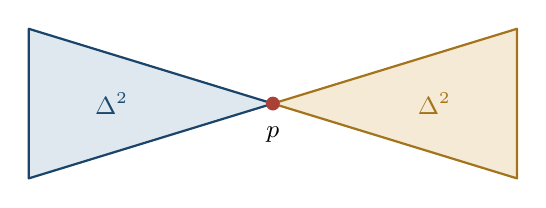
\begin{tikzpicture}[line cap=round,line join=round]
 \fill[manifoldblue!14] (-3.1,-.95)--(-3.1,.95)--(0,0)--cycle;
 \fill[manifoldgold!19] (0,0)--(3.1,.95)--(3.1,-.95)--cycle;
 \draw[manifoldblue!75!black,thick]
  (-3.1,-.95)--(-3.1,.95)--(0,0)--cycle;
 \draw[manifoldgold!80!black,thick]
  (0,0)--(3.1,.95)--(3.1,-.95)--cycle;
 \fill[manifoldred] (0,0) circle (2.5pt);
 \node[below=5pt,font=\small] at (0,0) {$p$};
 \node[font=\small,manifoldblue!80!black] at (-2.05,0) {$\Delta^2$};
 \node[font=\small,manifoldgold!80!black] at (2.05,0) {$\Delta^2$};
\end{tikzpicture}
\caption{Dwa trójkąty ze wspólnym wierzchołkiem $p$.
To kompleks symplicjalny, ale w $p$ nie jest
powierzchnią gładką, nawet z brzegiem.}
\label{fig:kompleks-nie-rozmaitosc}
\end{figure}

Homologia singularna idzie jeszcze dalej: jej
sympleksy są \emph{ciągłymi odwzorowaniami}
$\Delta^k\to X$, dlatego definiuje się ją
dla dowolnej przestrzeni topologicznej $X$,
również bez wybranej triangulacji. Kohomologia
de Rhama wymaga natomiast \emph{gładkiej
rozmaitości} $M$: żeby pisać formy i ich
różniczkę $\dd$, potrzebujemy przestrzeni
stycznych i gładkich odwzorowań. Dla kompleksu
z Rysunku~\ref{fig:kompleks-nie-rozmaitosc}
zwykła kohomologia de Rhama w sensie
Definicji~\ref{def:de-rham-cohomology}
nie jest zdefiniowana. Grupy homotopii
można z kolei definiować dla przestrzeni
topologicznych z wybranym punktem bazowym.

Do czego służą te niezmienniki, jeśli słowo
„dziura” nie daje jeszcze ścisłej odpowiedzi?
Pozwalają rozstrzygać, czy cykl jest brzegiem,
czy zamknięta forma jest różniczką innej formy,
czy pętlę albo odwzorowanie sfery można
ściągnąć do punktu. Pomagają też odróżnić
przestrzenie oraz badać odwzorowania między nimi.
Istotny jest zarówno obiekt, od którego
zaczynamy, jak i relacja uznająca dwa takie
obiekty za równoważne:

\begin{center}
\small
\renewcommand{\arraystretch}{1.18}
\begin{tabular}{>{\raggedright\arraybackslash}p{3.05cm}
                >{\raggedright\arraybackslash}p{4.4cm}
                >{\raggedright\arraybackslash}p{6.75cm}}
\hline
\textbf{Typ}&\textbf{Na czym konstruowana}&
\textbf{Co wykrywa i o czym mówi}\\
\hline
$H_k^{\mathrm{simp}}(K;\Z)$,
homologia symplicjalna&
Zorientowane sympleksy kompleksu $K$,
całkowite łańcuchy, operator brzegu
$\partial$; cykle modulo brzegi.&
Rozpoznaje składowe ($H_0$), klasy cykli,
które nie są brzegami, ich liczbę niezależnych
generatorów i torsję. Na zamkniętej spójnej
rozmaitości jej najwyższa homologia z $\Z$
pomaga rozpoznać orientowalność.\\
\hline
$H_k^{\mathrm{sing}}(X;\Z)$,
homologia singularna&
Wszystkie ciągłe odwzorowania
$\Delta^k\to X$ jako generatory łańcuchów;
ten sam operator $\partial$ i iloraz
cykli przez brzegi.&
Daje homologiczne informacje bez wybierania
triangulacji, dla dowolnej przestrzeni
topologicznej. Ciągłe $f:X\to Y$ wyznacza
$f_*:H_k(X)\to H_k(Y)$; można nim badać,
jak odwzorowanie przenosi klasy cykli.\\
\hline
$H^k_{\mathrm{dR}}(M)$,
kohomologia de Rhama&
Gładkie formy różniczkowe na rozmaitości $M$,
różniczka $\dd$; formy zamknięte modulo dokładne.&
Mówi, czy zamknięta forma ma \emph{globalnie}
formę pierwotną. Całki po cyklach mierzą jej
okresy; iloczyn zewnętrzny form pozwala badać
iloczyny klas. Zwykła wersja ma wartości
rzeczywiste, więc nie wykrywa torsji.\\
\hline
$\pi_1(X,p)$,
grupa podstawowa&
Pętle o początku i końcu w $p$;
utożsamiamy pętle homotopijne, a działaniem
jest ich składanie.&
Mówi, których pętli nie można ściągnąć do
punktu. Zawiera informację o nakryciach
i może być nieprzemienna; przez to odróżnia
przestrzenie o tym samym $H_1$.\\
\hline
$\pi_k(X,p)$, $k\geq2$,
wyższe grupy homotopii&
Odwzorowania sfer $S^k\to X$ z punktem
bazowym, modulo homotopia zachowująca
ten punkt.&
Mówią, czy odwzorowanie sfery można
ściągnąć do punktu (równoważnie: przedłużyć
na dysk $D^{k+1}$). Mogą być niezerowe,
nawet gdy $H_k(X;\Z)=0$.\\
\hline
\end{tabular}
\end{center}

Na przykład $H_1$ pozwala wykazać, że
nie istnieje retrakcja dysku $D^2$ na jego
brzeg $S^1$: gdyby $r:D^2\to S^1$
i inkluzja $i:S^1\to D^2$ spełniały
$r\circ i=\id$, to na homologii byłoby
$r_*\circ i_*=\id$ na $H_1(S^1;\Z)\cong\Z$.
Jest to niemożliwe, bo $H_1(D^2;\Z)=0$.
Kohomologia de Rhama rozstrzyga, czy da się
zbudować globalny potencjał dla zamkniętej
formy, a $\pi_1$ pomaga opisać nakrycia.
„Dziury” są więc tylko jednym z obrazowych
skrótów dla tych konkretnych pytań.

Różni się też koszt rachunku. Bez triangulacji
kompleks łańcuchów singularnych ma ogromnie
wiele generatorów. Skończona triangulacja
sprowadza homologię symplicjalną do macierzy
operatorów brzegu, lecz znalezienie odpowiedniej
triangulacji i obliczenie jąder oraz obrazów
bywa trudne. Formy pozwalają czasem wykorzystać
współrzędne i symetrie rozmaitości, choć
ustalenie, czy forma ma \emph{globalną}
formę pierwotną, także wymaga pracy.
Nie ma jednej metody zawsze najłatwiejszej.

\subsection*{Od sympleksów do całek}

W tej części $H_k^{\mathrm{simp}}$ oznacza tę samą homologię,
którą wcześniej zapisywaliśmy $H_k^\Delta$, a
$H_k^{\mathrm{sing}}$ to wcześniejsze $H_k$ przestrzeni.
Indeksy służą tylko odróżnieniu konstrukcji w porównaniu.
Dla triangulacji $K$ Twierdzenie
\ref{thm:symplicjalna-singularna} utożsamia
$H_k^{\mathrm{simp}}(K;\Z)$ z
$H_k^{\mathrm{sing}}(M;\Z)$: wynik nie zależy
od wyboru triangulacji, chociaż liczba i kształt
sympleksów od niej zależą. Dla nieskończonej, lokalnie
skończonej triangulacji stosujemy ten sam wynik do skończonych
podkompleksów: skończony łańcuch symplicjalny ma skończony
nośnik, a obraz każdego łańcucha singularnego jest zwarty,
więc spotyka tylko skończenie wiele sympleksów.
To dotyczy także łańcuchów wypełniających; izomorfizmy
na skończonych podkompleksach dają więc zarówno
surjektywność, jak i iniektywność porównania globalnego.
Cyklem jest łańcuch
$z$ z $\partial z=0$. Jeżeli $z=\partial c$,
to reprezentuje zero w homologii.
W najprostszym przykładzie trzy krawędzie
obwodu trójkąta tworzą $1$-cykl. Jeśli
pozostawimy sam obwód, nie ma $2$-sympleksu,
którego ten cykl byłby brzegiem, i
$H_1\cong\Z$. Jeśli dodamy wypełniony trójkąt,
ten sam cykl staje się jego brzegiem:
\[
 \partial[v_0v_1v_2]
 =[v_1v_2]-[v_0v_2]+[v_0v_1].
\]
Wtedy $H_1=0$. To dosłowny sens
„wykrycia dziury” przez homologię.
Na okręgu
jedno pełne obejście daje generator $H_1(S^1;\Z)
\cong\Z$; na $S^2$ cała zorientowana powierzchnia
daje generator $H_2(S^2;\Z)\cong\Z$.

Klasa zamkniętej formy przypisuje liczby
klasom cykli: całkujemy formę po cyklu.
Wybieramy przy tym gładkiego reprezentanta całej klasy
cyklu, co uzasadniono w dowodzie Twierdzenia~\ref{thm:de-rham}.
Taką liniową regułę przypisującą wektorom
liczby nazywamy \emph{funkcjonałem liniowym}.
Właśnie w tym sensie kohomologia de Rhama
wiąże się z homologią. Jeśli
$\dd\omega=0$ i $\partial z=0$, definiujemy
\begin{equation}\label{eq:parowanie-de-rham-homologia}
 \langle[\omega],[z]\rangle:=\int_z\omega.
\end{equation}
Zmiana $\omega$ o $\dd\eta$ zmienia całkę o
$\int_{\partial z}\eta=0$; zmiana $z$ o
$\partial c$ zmienia ją o
$\int_c\dd\omega=0$. Jest więc dobrze określona
na klasach po obu stronach. To dokładnie
rachunek Stokesa~\eqref{eq:integracja-lancuchowa}.

Czy \emph{każdą} funkcję liniową przypisującą
klasom homologii liczby rzeczywiste można
otrzymać przez całkowanie zamkniętej formy?
Twierdzenie de Rhama daje odpowiedź twierdzącą.
Aby zobaczyć, skąd bierze się ta odpowiedź,
pokażmy najpierw krok algebraiczny.
Dla kompleksu
łańcuchowego przestrzeni wektorowych nad $\R$
kołańcuch $c:C_k\to\R$ jest kocyklem
($\delta c=0$) dokładnie wtedy, gdy znika
na $B_k=\partial C_{k+1}$. Jego ograniczenie
do $Z_k=\ker(\partial:C_k\to C_{k-1})$ zależy
więc tylko od klasy w $H_k=Z_k/B_k$.
Jeżeli ten funkcjonał na $H_k$ jest zerowy,
to $c$ znika na całym $Z_k$. Definiujemy
na $B_{k-1}=\partial C_k$ funkcjonał
$b(\partial a):=c(a)$. Jest dobrze określony:
z $\partial a=\partial a'$ wynika
$a-a'\in Z_k$, a zatem $c(a)=c(a')$.
Rozszerzamy $b$ liniowo na $C_{k-1}$.
Wtedy $(\delta b)(a)=b(\partial a)=c(a)$,
czyli $c$ był kobrzegiem. Odwrotnie, każdy
funkcjonał $\lambda:H_k\to\R$ definiuje
funkcjonał na $Z_k$, który można liniowo
przedłużyć na $C_k$; ponieważ znika na
$B_k$, przedłużenie jest kocyklem.
Dowiedliśmy zatem
\[
 H^k_{\mathrm{sing}}(M;\R)
 \cong \operatorname{Hom}_{\R}
       (H_k^{\mathrm{sing}}(M;\R),\R).
\]
Symbol $\operatorname{Hom}_{\R}(V,\R)$ oznacza
przestrzeń \emph{wszystkich} funkcjonałów liniowych
$V\to\R$: każdy przypisuje wektorowi z $V$
liczbę rzeczywistą i zachowuje dodawanie
oraz mnożenie przez skalar.
Łącząc to z Twierdzeniem~\ref{thm:de-rham}
i porównaniem symplicjalnym, otrzymujemy
dla triangulowanej rozmaitości
\begin{equation}\label{eq:porownanie-simp-de-rham}
 H^k_{\mathrm{dR}}(M)
 \cong \operatorname{Hom}_{\R}
       (H_k^{\mathrm{simp}}(K;\R),\R),
\end{equation}
przy czym izomorfizm jest dany przez całkę
z~\eqref{eq:parowanie-de-rham-homologia}.
Jeśli grupy homologii są skończenie generowane,
wymiar $H^k_{\mathrm{dR}}$ to $k$-ta liczba
Betti'ego, czyli liczba swobodnych generatorów
$H_k(M;\Z)$. Forma nie zobaczy torsji: gdy
$nz=\partial c$ dla $n\ne0$, to dla zamkniętej
$\omega$ mamy
$n\int_z\omega=\int_c\dd\omega=0$,
więc $\int_z\omega=0$.

Wybór współczynników wyjaśnia tu ważną różnicę.
Według Twierdzenia~\ref{thm:homologia-char-zero}
przejście z $\Z$ do $\Q$, $\R$ lub $\C$
zachowuje liczby Betti'ego, lecz usuwa torsję;
Przykład~\ref{prz:zmiana-wspolczynnikow-rp2-torus}
pokazuje to dla $\mathbb{RP}^2$ i torusa.
Zwykły kompleks form de Rhama jest rzeczywisty
i oblicza $H^k_{\mathrm{sing}}(M;\R)$.
Jeśli dopuścimy formy zespolone,
$\Omega^\bullet(M;\C)
=\Omega^\bullet(M;\R)\otimes_{\R}\C$,
otrzymamy analogicznie
$H^k_{\mathrm{dR}}(M;\C)
\cong H^k_{\mathrm{dR}}(M;\R)\otimes_{\R}\C$.
Współczynniki $\Q$ stosujemy bezpośrednio
w łańcuchach i kołańcuchach singularnych;
nie wymagają one osobnej teorii gładkich
form o wymiernych współczynnikach.

\subsection*{Od sfer do cykli}

W tym porównaniu zakładamy, że $M$ jest spójna drogowo;
w przeciwnym razie pracujemy na składowej zawierającej $p$.
Element $\pi_k(M,p)$ jest klasą odwzorowania
$(S^k,*)\to(M,p)$. Po przeniesieniu generatora
$H_k(S^k;\Z)$ otrzymujemy klasę w $H_k(M;\Z)$:
to odwzorowanie Hurewicza $h_k$
z Rozdziału~\ref{ch:wyzsza-homotopia}.
W stopniu $1$ dokładna odpowiedź z
Twierdzenia~\ref{thm:hurewicz-h1} brzmi
\[
 H_1(M;\Z)\cong\pi_1(M,p)_{\mathrm{ab}}.
\]
Komutatory pętli znikają po przejściu
do homologii, ponieważ dodawanie cykli
jest przemienne; $\pi_1$ może być nieprzemienna.
W wyższych stopniach $h_k$ nie musi być
izomorfizmem. Dla $k\geq2$, gdy $M$ jest
$(k-1)$-spójna, Twierdzenie
\ref{thm:hurewicz-wyzszy} utożsamia
pierwszą możliwą niezerową grupę
$\pi_k(M)$ z $H_k(M;\Z)$.
Aby zastosować tu wersję twierdzenia dla kompleksów CW,
używamy dodatkowego twierdzenia o triangulacji gładkich
rozmaitości: każda taka rozmaitość dopuszcza lokalnie
skończoną triangulację, a przy brzegu można wybrać
$\partial M$ jako podkompleks. Sympleksy tej triangulacji
są komórkami CW. Istnienie triangulacji jest osobnym
wynikiem topologii różniczkowej, nie konsekwencją de Rhama;
jego dowód wykracza poza to porównanie. Źródło wskazano
w dalszej lekturze. W rozważanych przykładach okręgu,
sfer, torusa i przestrzeni rzutowej strukturę CW znamy
już jawnie z wcześniejszych rozdziałów.
Teza dotyczy właśnie pierwszego
niezerowego stopnia przy podanej spójności;
nie utożsamia wszystkich późniejszych grup.

\begin{przyklad}[Ta sama informacja w stopniu pierwszym]
Na $S^1$ zachodzi
$\pi_1(S^1)\cong H_1(S^1;\Z)\cong\Z$,
a $H^1_{\mathrm{dR}}(S^1)\cong\R$.
Klasa formy $\vartheta/(2\pi)$ z
Przykładu~\ref{prz:de-rham-s1} daje wartość
$1$ na dodatnim generatorze homologii.
Liczba całkowita zlicza okrążenia, a całka
z formy przypisuje im liczby rzeczywiste
w sposób liniowy.
\end{przyklad}

\begin{przyklad}[Ta sama pierwsza homologia,
różne grupy podstawowe]
Torus $T^2$ ma $\pi_1(T^2)\cong\Z^2$.
Jeśli usuniemy otwarty dysk o domknięciu zawartym
we wnętrzu jego dwuwymiarowej komórki,
otrzymamy zwartą powierzchnię z brzegiem
$P=T^2\setminus\operatorname{int}D^2$.
W modelu komórkowym z Przykładu
\ref{prz:pi1-torus-rp2} część
dwuwymiarowa po usunięciu dysku ściąga się
na część jednowymiarową $S^1\vee S^1$.
Dlatego $\pi_1(P)\cong F_2$, wolna
nieprzemienna grupa na dwóch generatorach,
podczas gdy $H_1(P;\Z)\cong\Z^2$.
Zarówno $P$, jak i $T^2$ mają więc
$H^1_{\mathrm{dR}}\cong\R^2$:
w stopniu pierwszym formy i homologia
nie wykrywają nieprzemienności $\pi_1(P)$.
Pełne grupy homologii tych przestrzeni
różnią się jednak w stopniu $2$:
$H_2(P;\Z)=0$, a $H_2(T^2;\Z)=\Z$.
\end{przyklad}

\begin{przyklad}[Informacja sferyczna bez klasy homologii]
Dla $\mathbb{RP}^2$ wcześniejsze obliczenia dają
\[
 \pi_1(\mathbb{RP}^2)=\Z/2,\qquad
 \pi_2(\mathbb{RP}^2)=\Z,\qquad
 H_1(\mathbb{RP}^2;\Z)=\Z/2,\qquad
 H_2(\mathbb{RP}^2;\Z)=0.
\]
Porównaj Przykłady~\ref{prz:rp2-pi2}
i~\ref{prz:homologia-rp2}. Nakrycie
$S^2\to\mathbb{RP}^2$ pozostawia nietrywialną
klasę w $\pi_2$, ale jej obraz przez $h_2$
jest zerowy. Dodatkowo
$H^k_{\mathrm{dR}}(\mathbb{RP}^2)=0$
dla każdego $k>0$: całki form nie wykryją
ani torsji w $H_1$, ani tej klasy sferycznej.
Jest to wyraźny przykład, dlaczego trzech teorii
nie wolno po prostu utożsamiać.
\end{przyklad}

\section*{Dalsza lektura}
\addcontentsline{toc}{section}{Dalsza lektura}
\href{https://ocw.mit.edu/courses/18-965-geometry-of-manifolds-fall-2004/pages/lecture-notes/}
{Notatki kursu \emph{Geometry of Manifolds} (MIT OpenCourseWare)},
wykłady o formach, twierdzeniu Stokesa i twierdzeniu de Rhama.
Zob. także \href{https://www.math.toronto.edu/mgualt/courses/17-1300/docs/17-1300-notes-13.pdf}
{notatki o formach różniczkowych i twierdzeniu Stokesa}
Uniwersytetu w Toronto.
Porównanie z homologią i homotopią rozwija
\href{https://pi.math.cornell.edu/~hatcher/AT/AT.pdf}
{Allen Hatcher, \emph{Algebraic Topology}},
rozdziały 2--4. Twierdzenie o triangulacji rozmaitości
gładkich omawia Jacob Lurie w notatkach
\href{https://www.math.ias.edu/~lurie/937notes/937Lecture3.pdf}
{\emph{Whitehead Triangulations}, wykład 3} i kolejnych
wykładach tego kursu.


\chapter{Tensor metryczny, długość i miara}
\label{ch:metryka-riemannowska}

Topologia mówi, które punkty są blisko w sensie otoczeń,
ale sama nie podaje długości odcinka ani pola powierzchni.
Na gładkiej rozmaitości możemy w każdym punkcie mierzyć
wektory styczne iloczynem skalarnym. Jeżeli taki pomiar
zmienia się gładko od punktu do punktu, otrzymujemy
\emph{tensor metryczny}. Z niego wyprowadzimy długość
krzywej, odległość punktów, pole podrozmaitości i objętość.
Na końcu połączymy te pojęcia z miarą Hausdorffa
i twierdzeniem Gaussa o dywergencji.

\section{Metryka w przestrzeniach stycznych}
\label{sec:metryka-definicja}

\begin{definicja}[Metryka riemannowska]
\index{metryka riemannowska@Metryka riemannowska}
\label{def:metryka-riemannowska}
Na gładkiej rozmaitości $M^n$ \emph{metryka riemannowska}
$g$ jest gładkim polem symetrycznych tensorów typu $(0,2)$
takim, że dla każdego $p\in M$ i $v\in T_pM\setminus\{0\}$
zachodzi $g_p(v,v)>0$. Piszemy
\[
 \langle v,w\rangle_{g,p}:=g_p(v,w),
 \qquad |v|_g:=\sqrt{g_p(v,v)}.
\]
Dla niezerowych $v,w$ kąt $\alpha$ wyznacza
$\cos\alpha=g_p(v,w)/(|v|_g|w|_g)$.
\end{definicja}

Intuicja: $g_p$ jest linijką i kątomierzem przyłożonym
do \emph{wektorów stycznych w punkcie $p$}. Nie porównuje
jeszcze bezpośrednio dwóch odległych punktów. Żeby to zrobić,
zsumujemy później długości maleńkich wektorów prędkości
wzdłuż krzywej. Współrzędne mogą deformować rysunek:
okrąg jednostkowych wektorów $g_p(v,v)=1$ bywa na kartce
elipsą. To zmiana opisu, nie zmiana pomiaru geometrycznego.

W mapie $x=(x^1,\ldots,x^n)$ zapisujemy
\begin{equation}\label{eq:metryka-macierz}
 g=\sum_{i,j=1}^n g_{ij}(x)\,\dd x^i\otimes\dd x^j,
 \qquad g_{ij}=g\!\left(\frac{\partial}{\partial x^i},
                          \frac{\partial}{\partial x^j}\right).
\end{equation}
Macierz $G=(g_{ij})$ jest symetryczna i dodatnio określona.
Zapis $g=g_{ij}\dd x^i\dd x^j$ jest skrótem
dla \eqref{eq:metryka-macierz}: nie chodzi tu o iloczyn
zewnętrzny form.

\begin{stwierdzenie}[Zmiana współrzędnych]
\label{prop:metryka-zmiana}
Jeżeli $x=x(y)$ na przecięciu dwóch map i
$J=(\partial x^i/\partial y^a)$, to
\[
 G_y=J^{\mathsf T}G_xJ,\qquad
 \det G_y=(\det J)^2\det G_x.
\]
\end{stwierdzenie}
\begin{proof}
Reguła łańcuchowa daje
$\partial/\partial y^a
 =\sum_i(\partial x^i/\partial y^a)\partial/\partial x^i$.
Wstawmy tę równość dwa razy do
$g(\partial/\partial y^a,\partial/\partial y^b)$.
Otrzymamy
$(G_y)_{ab}=\sum_{i,j}J_{ia}(G_x)_{ij}J_{jb}$,
czyli pierwszy wzór. Wyznacznik iloczynu macierzy
i $\det J^{\mathsf T}=\det J$ dają drugi.
W szczególności dodatnia określoność nie zależy
od wyboru współrzędnych: $w^{\mathsf T}G_yw
=(Jw)^{\mathsf T}G_x(Jw)>0$ dla $w\ne0$.
\end{proof}

\subsection*{Cofnięcie i przeniesienie metryki}
\label{subsec:metryka-pullback-pushforward}

Zapis $f^*h$ jest szczególnym przypadkiem cofnięcia
tensora z Definicji~\ref{def:cofniecie-tensora}.
Warto tu rozdzielić dwie czynności: \emph{cofnięcie}
metryki z przestrzeni docelowej na dziedzinę oraz
\emph{przeniesienie} metryki z dziedziny na cel przez
dyfeomorfizm. Nazwy angielskie to odpowiednio
\emph{pullback} i \emph{pushforward}.

\begin{definicja}[Pullback i pushforward metryki]
\index{pullback i pushforward metryki@Pullback i pushforward metryki}
\label{def:metryka-pullback-pushforward}
Niech $f:M\to N$ będzie gładkim odwzorowaniem, a $h$
metryką riemannowską na $N$. \emph{Cofnięty tensor}
$f^*h$ na $M$ jest określony przez
\begin{equation}\label{eq:metryka-pullback}
 (f^*h)_p(v,w)
 =h_{f(p)}(\dd f_pv,\dd f_pw),
 \qquad v,w\in T_pM.
\end{equation}
Jeśli $f$ jest immersją, $f^*h$ jest metryką
riemannowską, zwaną metryką indukowaną.

Jeżeli $f$ jest dyfeomorfizmem i $g$ jest metryką
na $M$, definiujemy \emph{przeniesioną metrykę}
na $N$ wzorem
\begin{equation}\label{eq:metryka-pushforward}
 (f_*g)_q(u,w)
 :=g_{f^{-1}(q)}(\dd(f^{-1})_q u,
                    \dd(f^{-1})_q w),
 \qquad f_*g=(f^{-1})^*g.
\end{equation}
\end{definicja}

W~\eqref{eq:metryka-pullback} dwa wektory z $T_pM$
przenosimy różniczką do $T_{f(p)}N$ i mierzymy tam
za pomocą $h$. Dlatego do cofnięcia tensora typu
$(0,2)$ \emph{nie} jest potrzebna odwrotność $f$.
Jeżeli $\dd f_p$ ma jądro, wektor $v\ne0$ z tego
jądra ma $(f^*h)_p(v,v)=0$; wtedy cofnięty tensor
nie jest metryką riemannowską. Na przykład dla
$f:\R^2\to\R$, $f(x,y)=x$, cofnięcie $\dd t^2$
to $\dd x^2$, które nie mierzy wektora $\partial_y$.
Przy pushforwardzie trzeba zaś umieć odtworzyć
jednoznacznie wektor w punkcie $f^{-1}(q)$;
dyfeomorfizm to gwarantuje.

\begin{stwierdzenie}[Co daje dyfeomorfizm?]
\label{prop:metryka-dyfeo-izometria}
Niech $f:M\to N$ będzie dyfeomorfizmem.
Wtedy $f^*h$ i $f_*g$ są metrykami riemannowskimi,
a operacje są wzajemnie odwrotne:
\[
 f^*(f_*g)=g,\qquad f_*(f^*h)=h.
\]
Dyfeomorfizm $f:(M,g)\to(N,h)$ jest izometrią
wtedy i tylko wtedy, gdy $f^*h=g$, równoważnie
$f_*g=h$. W tym przypadku zachowuje długości krzywych,
odległość punktów, kąty, geodezyjne i tensor krzywizny.
\end{stwierdzenie}
\begin{proof}
Jeśli $v\ne0$, to $\dd f_pv\ne0$, bo różniczka
dyfeomorfizmu jest odwracalna. Zatem
$(f^*h)_p(v,v)=h_{f(p)}(\dd f_pv,\dd f_pv)>0$;
gładkość i symetria wynikają ze wzoru.
Analogicznie jest dla $f_*g$. Równość
$\dd(f^{-1})_{f(p)}\circ\dd f_p=\mathrm{Id}$ daje
\[
 (f^*f_*g)_p(v,w)
 =(f_*g)_{f(p)}(\dd f_pv,\dd f_pw)
 =g_p(v,w).
\]
Po zamianie $f$ z $f^{-1}$ otrzymujemy drugą
tożsamość. Warunek $f^*h=g$ mówi dokładnie, że
$\dd f_p$ zachowuje iloczyn skalarny wszystkich
wektorów stycznych; jest to definicja izometrii.
Dla każdej odcinkami gładkiej krzywej $\gamma$
reguła łańcuchowa daje
\[
 L_h(f\circ\gamma)
 =\int\sqrt{h_{f(\gamma(t))}
             (\dd f\,\dot\gamma,\dd f\,\dot\gamma)}\,\dd t
 =\int\sqrt{g_{\gamma(t)}
             (\dot\gamma,\dot\gamma)}\,\dd t
 =L_g(\gamma).
\]
Ponieważ $f$ i $f^{-1}$ przenoszą wszystkie drogi
między odpowiednimi punktami, branie kresu dolnego
ich długości daje $d_h(f(p),f(q))=d_g(p,q)$.
Twierdzenia o zachowaniu geodezyjnych i krzywizny są
zapowiedzią pojęć z dwóch następnych rozdziałów.
Poniższy akapit można przeczytać po poznaniu koneksji
Leviego-Civity i definicji krzywizny; pozostała część
obecnego rozdziału nie korzysta z tych dwóch własności.
Sprawdźmy je, używając wskazanych tam definicji. Dla pól na $M$ połóżmy
\[
 \widetilde\nabla_XY
 :=f^{-1}_*\bigl(\nabla^h_{f_*X}(f_*Y)\bigr).
\]
Ponieważ $f_*[X,Y]=[f_*X,f_*Y]$, torsja tej
koneksji jest zerowa. Zgodność $\nabla^h$ z $h$
oraz $g(Y,Z)=h(f_*Y,f_*Z)\circ f$ daje
\[
 Xg(Y,Z)=g(\widetilde\nabla_XY,Z)
             +g(Y,\widetilde\nabla_XZ).
\]
Z jednoznaczności w Twierdzeniu~\ref{thm:levi-civita}
wynika $\widetilde\nabla=\nabla^g$. Stąd
$f_*(\nabla^g_{\dot\gamma}\dot\gamma)
=\nabla^h_{(f\circ\gamma)'}(f\circ\gamma)'$,
więc obrazy geodezyjnych są geodezyjnymi.
Podstawienie tej równości do definicji~\eqref{eq:riemann-def}
pokazuje, że $\dd f_p$ przenosi też operator krzywizny.
\end{proof}

W mapach, jeśli $J_f$ jest macierzą różniczki $f$,
to~\eqref{eq:metryka-pullback} przyjmuje postać
\[
 G_{f^*h}(x)=J_f(x)^{\mathsf T}H(f(x))J_f(x).
\]
W szczególności wzór
$G_y=J^{\mathsf T}G_xJ$ ze
Stwierdzenia~\ref{prop:metryka-zmiana} jest
cofnięciem \emph{tej samej} metryki przy zmianie
współrzędnych. Współczynniki się zmieniają, lecz
odległości mierzone na rozmaitości pozostają te same.

\begin{przyklad}[Dwa kierunki przekształcenia]
\label{prz:metryka-pull-push-przyklad}
Dyfeomorfizm $f:\R^2_{u,v}\to\R^2_{x,y}$,
$f(u,v)=(u,v+u^2)$, ma odwrotność
$f^{-1}(x,y)=(x,y-x^2)$. Cofając metrykę
euklidesową przestrzeni docelowej, znajdujemy
\[
 f^*(\dd x^2+\dd y^2)
 =\dd u^2+(\dd v+2u\,\dd u)^2.
\]
Przenosząc w przeciwną stronę metrykę euklidesową
dziedziny, dostajemy
\[
 f_*(\dd u^2+\dd v^2)
 =\dd x^2+(\dd y-2x\,\dd x)^2.
\]
To \emph{dwie różne} metryki zapisane na dwóch
różnych dziedzinach. Pierwsza sprawia, że
$f:(\R^2,f^*h_{\mathrm E})\to(\R^2,h_{\mathrm E})$
jest izometrią; druga sprawia, że
$f:(\R^2,g_{\mathrm E})\to(\R^2,f_*g_{\mathrm E})$
jest izometrią. Choć współczynniki zależą od punktu,
obie są płaskie, bo powstały przez przeniesienie
metryki euklidesowej.
\end{przyklad}

\begin{twierdzenie}[Istnienie metryki riemannowskiej]
\label{thm:istnienie-metryki}
Każda gładka rozmaitość Hausdorffa o przeliczalnej bazie,
również z brzegiem, ma metrykę riemannowską.
\end{twierdzenie}
\begin{proof}
Wybierzmy pokrycie mapami $(U_\alpha,x_\alpha)$.
W każdej mapie przenieśmy standardowy iloczyn skalarny
z $\R^n$ na wektory styczne:
\[
 (g_\alpha)_p(v,w)
 =\sum_{i=1}^n
   \dd x_\alpha^i{}_p(v)\,\dd x_\alpha^i{}_p(w).
\]
To dodatnio określony, gładki tensor na $U_\alpha$,
bo $\dd x_{\alpha,p}:T_pM\to\R^n$ jest izomorfizmem.
Twierdzenie~\ref{thm:podzial-jednosci-formy}
daje gładki podział jedności $(\rho_j)$
z $\supp\rho_j\subset U_{\alpha(j)}$.
Każdy tensor $\rho_jg_{\alpha(j)}$ przedłużamy przez
zero poza odpowiadającą mu mapę i kładziemy
$g=\sum_j\rho_jg_{\alpha(j)}$.
Suma jest lokalnie skończona, zatem gładka.
Jeżeli $v\ne0$ w punkcie $p$, to dla wszystkich $j$
składniki $\rho_j(p)(g_{\alpha(j)})_p(v,v)$ są
nieujemne, a przynajmniej jeden jest dodatni:
$\sum_j\rho_j(p)=1$, więc istnieje $j$ z
$\rho_j(p)>0$. Stąd $g_p(v,v)>0$.
Ta sama konstrukcja działa w mapach przybrzegowych.
\end{proof}

Twierdzenie zapewnia \emph{istnienie}, nie wskazuje
jednego wyróżnionego wyboru. Na przykład na $\R^n$, $n\geq1$,
metryki $\sum_i(\dd x^i)^2$ i
$e^{2f(x)}\sum_i(\dd x^i)^2$ są różne dla
niezerowej funkcji gładkiej $f$. Druga mnoży
długości wektorów w $x$ przez $e^{f(x)}$,
a objętości $n$-wymiarowe przez $e^{nf(x)}$.

\section{Geometrie modelowe}
\label{sec:metryki-modelowe}

\begin{przyklad}[Przestrzeń euklidesowa]
Na $\R^n$ bierzemy $g_{\mathrm E}=\sum_i(\dd x^i)^2$.
Wtedy $G=I_n$ i $|v|_g=\sqrt{\sum_i(v^i)^2}$.
To punkt odniesienia dla kolejnych modeli.
\end{przyklad}

\begin{przyklad}[Sfera]
\label{prz:metryka-sfery}
Dla $R>0$ sfera $S_R^2=\{x\in\R^3:|x|=R\}$ otrzymuje
metrykę przez ograniczenie euklidesowego iloczynu
skalarnego do $T_pS_R^2$. Parametryzacja
\[
 F(\theta,\phi)
 =R(\sin\theta\cos\phi,\sin\theta\sin\phi,\cos\theta)
\]
ma wektory pochodne
\[
 F_\theta
 =R(\cos\theta\cos\phi,\cos\theta\sin\phi,-\sin\theta),
 \quad
 F_\phi
 =R(-\sin\theta\sin\phi,\sin\theta\cos\phi,0).
\]
Ich iloczyny skalarne wynoszą kolejno
$R^2$, $0$ i $R^2\sin^2\theta$. Zatem
\begin{equation}\label{eq:metryka-sfery}
 g_{S_R^2}=R^2\dd\theta^2
       +R^2\sin^2\theta\,\dd\phi^2.
\end{equation}
Długość przy zmianie samego kąta biegunowego
$\theta$ jest inna niż przy zmianie $\phi$ blisko
bieguna: równoleżniki stają się tam krótkie.
Zanik $\sin\theta$ na biegunie nie oznacza
degeneracji metryki; współrzędna $\phi$ nie jest
tam poprawną współrzędną lokalną.

Dla $S_R^n$ współrzędne stereograficzne $u\in\R^n$
z mapą odwrotną
\[
 s(u)=\left(\frac{2R^2u}{R^2+|u|^2},
            R\frac{|u|^2-R^2}{R^2+|u|^2}\right)
\]
dają
\begin{equation}\label{eq:metryka-stereograficzna}
 s^*g_{S_R^n}
 =\left(\frac{2R^2}{R^2+|u|^2}\right)^2
   \sum_i(\dd u^i)^2.
\end{equation}
Rzeczywiście, dla $q=R^2+|u|^2$ i wektora $h$
różniczka dwóch składowych $s$ ma postać
\[
 \dd s_u(h)=
 \left(\frac{2R^2h}{q}
       -\frac{4R^2u(u\cdot h)}{q^2},
       \frac{4R^3(u\cdot h)}{q^2}\right).
\]
W kwadracie normy wyrazy zawierające
$(u\cdot h)^2$ znoszą się, a zostaje
$4R^4|h|^2/q^2$. Spolaryzowanie tej
równości daje \eqref{eq:metryka-stereograficzna}.
\end{przyklad}

\begin{przyklad}[Trzy modele przestrzeni hiperbolicznej]
\label{prz:trzy-modele-hiperboliczne}
Niech $n\geq2$. W \emph{modelu półprzestrzeni}
punkty mają współrzędne $(x,y)\in\R^{n-1}\times(0,\infty)$,
a metryka jest
\begin{equation}\label{eq:hip-polprzestrzen}
 g_{\mathbb H}=\frac{|\,\dd x\,|^2+\dd y^2}{y^2}.
\end{equation}
Przy małej wysokości $y$ ten sam ruch euklidesowy
staje się długi hiperbolicznie.

W \emph{modelu kuli Poincarégo} $B^n=\{|u|<1\}$,
\begin{equation}\label{eq:hip-kula}
 g_B=\frac{4\sum_i(\dd u^i)^2}{(1-|u|^2)^2}.
\end{equation}
Brzeg kuli nie należy do przestrzeni. Wreszcie
\emph{model hiperboloidy} jest górnym płatem
\[
 \mathcal H^n=\{(t,z)\in\R\times\R^n:
                    t^2-|z|^2=1,\ t>0\}
\]
z ograniczeniem formy $-\dd t^2+\sum_i(\dd z^i)^2$
do wektorów stycznych. Choć forma w otoczeniu
ma znak minus, jej ograniczenie do $T\mathcal H^n$
jest dodatnio określone. Jeśli $(a,w)$ jest styczny,
to $ta=z\cdot w$ i
\[
 |w|^2-a^2
 =|w|^2-\frac{(z\cdot w)^2}{t^2}
 \geq\frac{|w|^2}{t^2}>0
 \quad\text{dla }(a,w)\ne0.
\]
Możemy także opisać hiperboloidę \emph{samymi
współrzędnymi przestrzennymi} $z\in\R^n$:
\begin{equation}\label{eq:hiperboloida-wspolrzedne-metryka}
 Q(z)=(\sqrt{1+|z|^2},z),\qquad
 (g_{\mathcal H})_{ij}
   =\delta_{ij}-\frac{z_i z_j}{1+|z|^2}.
\end{equation}
Istotnie, dla $t(z)=\sqrt{1+|z|^2}$ mamy
$\partial_i t=z_i/t$, toteż ograniczenie
$-\dd t^2+|\dd z|^2$ do wykresu $Q$ daje
\eqref{eq:hiperboloida-wspolrzedne-metryka}.
Na wektorach prostopadłych do $z$ macierz $G$
ma wartość własną $1$, a w kierunku $z$
wartość $1/(1+|z|^2)$. Stąd, również przy $z=0$
przez ciągłość,
\begin{equation}\label{eq:hiperboloida-macierz-odwrotna}
 G^{-1}=I+zz^{\mathsf T},\qquad
 \det G=\frac1{1+|z|^2}.
\end{equation}
Równość dla macierzy odwrotnej można sprawdzić
mnożąc $(I-zz^{\mathsf T}/t^2)(I+zz^{\mathsf T})$
i używając $t^2=1+|z|^2$.

\emph{Dlaczego to ta sama geometria?}
Odwzorowanie
\[
 P:B^n\longrightarrow\mathcal H^n,\qquad
 P(u)=\left(\frac{1+|u|^2}{1-|u|^2},
            \frac{2u}{1-|u|^2}\right)
\]
ma odwrotność $u=z/(t+1)$.
Dla $q=1-|u|^2$ różniczkujemy:
\[
 \dd t=\frac{4(u\cdot\dd u)}{q^2},
 \qquad
 \dd z=\frac{2\,\dd u}{q}
          +\frac{4u(u\cdot\dd u)}{q^2}.
\]
Po podniesieniu do kwadratu w
$|\,\dd z\,|^2-\dd t^2$ współczynnik przy
$(u\cdot\dd u)^2$ jest
$16(q+|u|^2-1)/q^4=0$. Pozostaje dokładnie
$4|\,\dd u\,|^2/q^2$, czyli $P^*g_{\mathcal H}=g_B$.

Kula przechodzi na półprzestrzeń przez
\[
 F(u)=\left(\frac{2v}{D},\frac{1-|u|^2}{D}\right),
 \quad u=(v,s),\quad D=|v|^2+(s-1)^2.
\]
Jest to dyfeomorfizm: dla $(x,y)$ z $y>0$
odwrotność ma postać
\[
 F^{-1}(x,y)=
 \left(\frac{2x}{E},
       \frac{|x|^2+y^2-1}{E}\right),
 \quad E=|x|^2+(y+1)^2.
\]
Aby sprawdzić metrykę bez długiego rozwijania,
zauważmy, że $F$ jest złożeniem przesunięcia,
inwersji $w\mapsto w/|w|^2$, jednokładności
o skali $2$ i odbicia. Różniczka inwersji to
$|w|^{-2}(I-2ww^{\mathsf T}/|w|^2)$;
macierz w nawiasie jest ortogonalna.
Zatem $|\,\dd F_u(h)\,|=2|h|/D$.
Współrzędna wysokości wynosi
$y=(1-|u|^2)/D$, więc
\[
 F^*g_{\mathbb H}(h,h)
 =\frac{4|h|^2/D^2}{(1-|u|^2)^2/D^2}
 =g_B(h,h).
\]
Oba odwzorowania zachowują więc długości
wektorów i krzywych. Sfera i przestrzeń
hiperboliczna są zakrzywione inaczej;
formalny opis ich krzywizny odłożymy do
rozdziału o tensorze krzywizny.
\end{przyklad}

\begin{figure}[H]
\centering
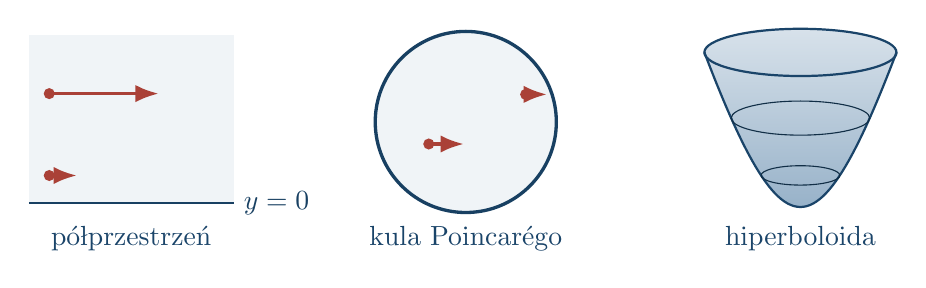
\begin{tikzpicture}[>=Latex,scale=1]
  \begin{scope}[shift={(-4.25,0)}]
    \fill[manifoldblue!7] (-1.3,-1.03) rectangle (1.3,1.10);
    \draw[manifoldblue!70!black,thick] (-1.3,-1.03)--(1.3,-1.03)
      node[right] {$y=0$};
    \fill[manifoldred] (-1.04,-.68) circle (2pt);
    \draw[manifoldred,very thick,->] (-1.04,-.68)--(-.69,-.68);
    \fill[manifoldred] (-1.04,.36) circle (2pt);
    \draw[manifoldred,very thick,->] (-1.04,.36)--(.35,.36);
    \node[manifoldblue!75!black] at (0,-1.48)
       {półprzestrzeń};
  \end{scope}
  \begin{scope}[shift={(0,0)}]
    \fill[manifoldblue!7] (0,0) circle (1.15);
    \draw[manifoldblue!70!black,very thick] (0,0) circle (1.15);
    \fill[manifoldred] (-.47,-.28) circle (2pt);
    \pgfmathsetmacro{\vlen}{1.15*(1-(.47*.47+.28*.28)/(1.15*1.15))/2}
    \draw[manifoldred,very thick,->] (-.47,-.28)--({-.47+\vlen},-.28);
    \fill[manifoldred] (.76,.35) circle (2pt);
    \pgfmathsetmacro{\vlen}{1.15*(1-(.76*.76+.35*.35)/(1.15*1.15))/2}
    \draw[manifoldred,very thick,->] (.76,.35)--({.76+\vlen},.35);
    \node[manifoldblue!75!black] at (0,-1.48)
       {kula Poincarégo};
  \end{scope}
  \begin{scope}[shift={(4.25,-.05)}]
    \pgfmathsetmacro{\htop}{3.4*(sqrt(1+1.22*1.22)-1)-1.03}
    \shade[top color=manifoldblue!18,bottom color=manifoldblue!47]
      plot[domain=-1.22:1.22,samples=61]
        (\x,{3.4*(sqrt(1+\x*\x)-1)-1.03})
      arc[start angle=0,end angle=180,x radius=1.22,y radius=.30]
      --cycle;
    \draw[manifoldblue!75!black,thick]
      plot[domain=-1.22:1.22,samples=61]
        (\x,{3.4*(sqrt(1+\x*\x)-1)-1.03});
    \draw[manifoldblue!75!black,thick] (0,\htop)
      ellipse (1.22 and .30);
    \foreach \rad in {.50,.88}{
      \pgfmathsetmacro{\height}{3.4*(sqrt(1+\rad*\rad)-1)-1.03}
      \draw[manifoldblue!50!black,thin] (0,\height)
        ellipse ({\rad} and {.246*\rad});
    }
    \node[manifoldblue!75!black] at (0,-1.43)
       {hiperboloida};
  \end{scope}
\end{tikzpicture}
\caption{Trzy zapisy tej samej geometrii hiperbolicznej. Czerwone strzałki przedstawiają wektory o długości hiperbolicznej $1$: taki wektor ma różną długość na euklidesowym rysunku półprzestrzeni i kuli. Linia $y=0$ oraz okrąg brzegowy nie należą do rozmaitości. Rysunek hiperboloidy przedstawia fragment górnego płata; jego profil jest gładki także w najniższym punkcie.}
\label{fig:metryki-trzy-modele-hiperboliczne}
\end{figure}

\section{Metryki Schwarzschilda i Kerra: inne znaki}
\label{sec:metryki-lorentzowskie}

\begin{definicja}[Metryka lorentzowska]
\index{metryka lorentzowska@Metryka lorentzowska}
\label{def:metryka-lorentzowska}
Metryka pseudoriemannowska jest gładkim,
symetrycznym, \emph{niezdegenerowanym} tensorem
typu $(0,2)$; dopuszczamy ujemne wartości $g(v,v)$.
W czterech wymiarach metryka o jednym kierunku
ujemnym i trzech dodatnich ma sygnaturę $(-,+,+,+)$
i nazywa się \emph{lorentzowską}.
\end{definicja}

Tu słowo „metryka” oznacza tensor, a nie funkcję
odległości na parach punktów. Dla wektora
czasopodobnego $v$ może być $g(v,v)<0$, a dla
niezerowego wektora światłopodobnego $g(v,v)=0$.
Wzory na riemannowską długość i odległość
z następnej sekcji nie stosują się do całej
takiej czasoprzestrzeni.

W poniższych dwóch przykładach używamy jednostek
geometrycznych $G=c=1$. W jednostkach fizycznych
parametr masy ma wymiar długości:
$M=G M_{\mathrm{fiz}}/c^2$, gdzie
$M_{\mathrm{fiz}}$ jest masą ciała, $G$ stałą
grawitacji, a $c$ prędkością światła. Współrzędna
$t$ ma wtedy wymiar długości ($t=c\,t_{\mathrm{fiz}}$).
Kąty $\theta\in(0,\pi)$ i $\phi\pmod{2\pi}$
oznaczają odpowiednio kąt od osi obrotu oraz azymut.
Symbole $\dd t^2$, $\dd r^2$ itd. oznaczają
kwadraty różniczek współrzędnych w zapisie
symetrycznego tensora $g$.

\begin{przyklad}[Schwarzschild]
\label{prz:metryka-schwarzschild}
W jednostkach geometrycznych $G=c=1$, dla $M>0$
i na obszarze zewnętrznym $r>2M$, metryka ma postać
\begin{equation}\label{eq:schwarzschild}
 g_{\mathrm{Sch}}
 =-\left(1-\frac{2M}{r}\right)\dd t^2
  +\left(1-\frac{2M}{r}\right)^{-1}\dd r^2
  +r^2\bigl(\dd\theta^2+\sin^2\theta\,\dd\phi^2\bigr).
\end{equation}
Parametr $M$ opisuje masę źródła, natomiast $r$
jest \emph{promieniem powierzchniowym}:
sfera określona przez $t,r=\mathrm{const}$
ma pole $4\pi r^2$. Nie jest to ogólnie odległość
zmierzona wzdłuż promienia; z metryki na
$t=\mathrm{const}$ odczytujemy element takiej
odległości $\dd\ell=\dd r/\sqrt{1-2M/r}$.
Współrzędna $t$ jest unormowana tak, aby asymptotycznie, gdy
$r\to\infty$, zgadzać się z czasem własnym obserwatorów
statycznych po przeliczeniu jednostek. Dla obserwatora
o stałych $r,\theta,\phi$ odczytujemy z metryki
$\dd\tau=\sqrt{1-2M/r}\,\dd t$; przy skończonym $r$
czas własny $\tau$ różni się więc od $t$.
Przy $r>2M$ współczynnik $\dd t^2$ jest ujemny,
a trzy przestrzenne są dodatnie, więc sygnatura
wynosi $(-,+,+,+)$. Dla ustalonego $t$
otrzymujemy \emph{riemannowską} metrykę przestrzennego
przekroju
\[
 h_{\mathrm{Sch}}
 =\left(1-\frac{2M}{r}\right)^{-1}\dd r^2
  +r^2\bigl(\dd\theta^2+\sin^2\theta\,\dd\phi^2\bigr).
\]
Na sferze $t,r=\mathrm{const}$ metryka indukowana
to \eqref{eq:metryka-sfery} z $R=r$, więc jej
pole wynosi $4\pi r^2$. Współrzędne sferyczne
nie działają na biegunach, a postać
\eqref{eq:schwarzschild} nie obejmuje $r=2M$;
odpowiednie przedłużenie opisuje się innymi
współrzędnymi.
\end{przyklad}

\begin{przyklad}[Kerr]
\label{prz:metryka-kerr}
Przy $M>0$, $|a|\leq M$ i
$r>r_+:=M+\sqrt{M^2-a^2}$ połóżmy
$\Sigma=r^2+a^2\cos^2\theta$ i
$\Delta=r^2-2Mr+a^2$. W zewnętrznej
dziedzinie współrzędnych Boyera--Lindquista
metrykę zapisuje się zwięźle jako
\begin{align}\label{eq:kerr}
 g_{\mathrm K}
 ={}&-\frac{\Delta}{\Sigma}
       (\dd t-a\sin^2\theta\,\dd\phi)^2
  +\frac{\sin^2\theta}{\Sigma}
       \bigl((r^2+a^2)\dd\phi-a\,\dd t\bigr)^2\\
 &+\frac{\Sigma}{\Delta}\dd r^2
  +\Sigma\,\dd\theta^2.\notag
\end{align}
Tutaj $M$ ponownie jest parametrem masy,
$J$ oznacza moment pędu źródła, a
$a=J/M$ w jednostkach $G=c=1$ jest parametrem
\emph{obrotu} o wymiarze długości
(w zwykłych jednostkach $a=J_{\mathrm{fiz}}/
(M_{\mathrm{fiz}}c)$). Znak $a$ ustala zwrot
obrotu względem rosnącego $\phi$; $a=0$ daje
przypadek bez obrotu. Założenie $|a|\leq M$
zapewnia rzeczywiste pierwiastki $\Delta=0$;
$r_+$ jest większym z nich, czyli współrzędną
zewnętrznego horyzontu. Wielkości $\Sigma$ i
$\Delta$ są skrótami zależnymi od współrzędnych,
nie dodatkowymi parametrami. Współrzędna $r$
nie mierzy tu odległości przestrzennej i przy
$a\ne0$ nie jest także promieniem sfery o polu
$4\pi r^2$; $t,\theta,\phi$ są współrzędnymi
Boyera--Lindquista. Wzór opisuje zewnętrze
horyzontu, a nie całą czasoprzestrzeń.
Kwadrat nawiasu jest kwadratem symetrycznym
$1$-formy. Ponieważ $\Delta>0$ dla $r>r_+$
i $0<\theta<\pi$, cztery wyświetlone
kwadraty mają odpowiednio znaki $-,+,+,+$
(po liniowo niezależnej zamianie pary
$\dd t,\dd\phi$). Istotnie, macierz tej zamiany to
$\left(\begin{smallmatrix}1&-a\sin^2\theta\\-a&r^2+a^2\end{smallmatrix}\right)$,
a jej wyznacznik wynosi $r^2+a^2\cos^2\theta=\Sigma>0$. W szczególności nie jest
to metryka riemannowska.

Sprawdźmy związek ze Schwarzschildem:
dla $a=0$ mamy $\Sigma=r^2$ oraz
$\Delta=r^2(1-2M/r)$; cztery składniki
\eqref{eq:kerr} stają się dokładnie
składnikami \eqref{eq:schwarzschild}.
Dla $a\ne0$ rozwinięcie dwóch pierwszych
kwadratów daje wyraz mieszany
\[
 -\frac{4Mar\sin^2\theta}{\Sigma}
      \,\dd t\,\dd\phi.
\]
W macierzy tensora oznacza to
$g_{t\phi}=-2Mar\sin^2\theta/\Sigma$:
oba wyrazy $g_{t\phi}\dd t\otimes\dd\phi$
i $g_{\phi t}\dd\phi\otimes\dd t$ składają
się na współczynnik podwojony.
Ten wyraz wiąże czas z kierunkiem obrotu.
Przekrój $t=\mathrm{const}$ ma dodatnio określoną
metrykę w podanej dziedzinie. Współczynniki przy
$\dd r^2$ i $\dd\theta^2$ są dodatnie, a współczynnik
przy $\dd\phi^2$ wynosi
\[
 \frac{\sin^2\theta}{\Sigma}
 \bigl((r^2+a^2)^2-a^2\Delta\sin^2\theta\bigr)>0,
\]
ponieważ wyrażenie w nawiasie równa się
$(r^2+a^2)\Sigma+2Mr a^2\sin^2\theta$.
Pomiary przestrzenne zależą jednak od wybranego
przekroju czasoprzestrzeni.
\end{przyklad}

W obu przykładach zapisaliśmy konkretne tensory
i sprawdziliśmy ich znaki oraz prostą zależność
między nimi. Ich wyprowadzenie z równań Einsteina
wymaga aparatu krzywizny, którego jeszcze nie
wprowadziliśmy.

\section{Długość, energia i odległość}
\label{sec:metryka-dlugosc-energia}

\begin{definicja}[Długość i energia krzywej]
\index{dlugosc i energia krzywej@Długość i energia krzywej}
\label{def:dlugosc-energia}
Niech $a<b$, a $\gamma:[a,b]\to(M,g)$ będzie ciągła
i odcinkami klasy $C^1$ (na skończonym podziale przedziału).
Wektor prędkości to $\dot\gamma(t)$, a jego długość,
nazywana także szybkością, wynosi $|\dot\gamma(t)|_g$.
Jej \emph{długość} i
\emph{energia} to odpowiednio
\begin{equation}\label{eq:dlugosc-energia}
 L_g(\gamma)=\int_a^b|\dot\gamma(t)|_g\,\dd t,
 \qquad
 E_g(\gamma)=\frac12\int_a^b
                  |\dot\gamma(t)|_g^2\,\dd t.
\end{equation}
Dla krzywych łączących $p$ z $q$ definiujemy
\begin{equation}\label{eq:odleglosc-riemannowska}
 d_g(p,q)=\inf_{\gamma(a)=p,\ \gamma(b)=q}
                 L_g(\gamma).
\end{equation}
Infimum bierzemy po krzywych odcinkami $C^1$.
Jeśli nie ma takiej krzywej, przyjmujemy $\inf\varnothing=+\infty$.
Zatem dla rozmaitości niespójnej wzór daje metrykę
skończoną osobno na każdej składowej; między różnymi
składowymi ma wartość $+\infty$.
\end{definicja}

Metryka $g$ mierzy wektor prędkości w każdym
punkcie, długość sumuje te pomiary wzdłuż
\emph{jednej} drogi, a $d_g$ szuka najkrótszej
możliwej długości. Infimum nie zakłada jeszcze,
że istnieje krzywa, która je osiąga.

\begin{stwierdzenie}[Zmiana parametru i energia]
\label{prop:energia-dlugosc}
Jeśli $h:[c,d]\to[a,b]$ jest rosnącym dyfeomorfizmem
klasy $C^1$, to
$L_g(\gamma\circ h)=L_g(\gamma)$.
Ponadto
\begin{equation}\label{eq:energia-cauchy}
 L_g(\gamma)^2\leq 2(b-a)E_g(\gamma),
\end{equation}
z równością wtedy i tylko wtedy, gdy prędkość
$|\dot\gamma|_g$ jest stała prawie wszędzie.
Dla regularnej krzywej klasy $C^1$, czyli takiej, że
$\dot\gamma(t)\ne0$, istnieje przeparametryzowanie klasy
$C^1$ ze stałą szybkością. Osiąga ono najmniejszą energię
wśród wszystkich regularnych przeparametryzowań na
ustalonym $[a,b]$. Dla krzywej odcinkami regularnej
odpowiednie przeparametryzowanie jest odcinkami klasy $C^1$.
\end{stwierdzenie}
\begin{proof}
Reguła łańcuchowa daje
$(\gamma\circ h)'(s)=\dot\gamma(h(s))h'(s)$.
Ponieważ $h'>0$, jednorodność normy i podstawienie
$t=h(s)$ dają
\[
 L_g(\gamma\circ h)
 =\int_c^d|\dot\gamma(h(s))|_g h'(s)\,\dd s
 =\int_a^b|\dot\gamma(t)|_g\,\dd t.
\]
Dla malejącego dyfeomorfizmu ten sam rachunek używa
$|h'|=-h'$ i odwróconych granic całkowania, więc długość
także się nie zmienia. Dla energii w pierwszej całce występuje
$(h')^2$, a więc podstawienie nie usuwa całego
czynnika: energia na ogół się zmienia.
Nierówność Cauchy'ego--Schwarza dla funkcji
$1$ i $|\dot\gamma|_g$ na $[a,b]$ daje
\[
 \left(\int_a^b|\dot\gamma|_g\,\dd t\right)^2
 \leq\left(\int_a^b1\,\dd t\right)
      \left(\int_a^b|\dot\gamma|_g^2\,\dd t\right).
\]
To \eqref{eq:energia-cauchy}. Warunek równości
w Cauchym--Schwarzu oznacza, że obie funkcje
są proporcjonalne prawie wszędzie, czyli
$|\dot\gamma|_g$ jest stała prawie wszędzie.
Dla regularnej krzywej $|\dot\gamma|_g>0$;
funkcja
$s(t)=a+\frac{b-a}{L_g(\gamma)}
               \int_a^t|\dot\gamma(\tau)|_g\,\dd\tau$
jest rosnąca, przenosi końce przedziału na
siebie, a reguła łańcuchowa pokazuje,
że $\gamma\circ s^{-1}$ ma stałą prędkość
$L_g(\gamma)/(b-a)$. Osiąga zatem dolną granicę
energii $L_g(\gamma)^2/[2(b-a)]$.
\end{proof}

\begin{twierdzenie}[Odległość riemannowska jest metryką]
\label{thm:odleglosc-jest-metryka}
Jeżeli $M$ jest spójna, to \eqref{eq:odleglosc-riemannowska}
przyjmuje skończone wartości, spełnia aksjomaty
metryki przestrzeni metrycznej $(M,d_g)$
i wyznacza pierwotną topologię rozmaitości.
\end{twierdzenie}
\begin{proof}
W wymiarze $0$ spójna rozmaitość składa się z jednego
punktu i teza jest natychmiastowa. Załóżmy $n\geq1$.
Relacja „można połączyć krzywą odcinkami $C^1$” jest
relacją równoważności. Każda jej klasa jest otwarta:
w małej kuli współrzędnych, a przy brzegu w półkuli,
można połączyć dwa punkty odcinkiem prostym w mapie.
Dopełnienie klasy także jest otwarte, jako suma innych
klas. Ze spójności wynika, że jest tylko jedna klasa.
Na każdym ze skończenie wielu kawałków takiej krzywej
prędkość i współczynniki metryki są ciągłe na zwartym
przedziale, więc długość jest skończona.
Zatem $d_g(p,q)<\infty$.

Długości są nieujemne, stała krzywa ma
długość zero, odwrócenie kierunku zachowuje
długość, a długości sklejonych krzywych
dodają się. Biorąc infima (i drogi o długości
dowolnie bliskiej obu infimom), otrzymujemy
$d_g(p,p)=0$, symetrię i nierówność trójkąta.

Zostało najważniejsze: $d_g(p,q)>0$ dla $p\ne q$.
Wybierzmy mapę $x$ z $x(p)=0$ i domkniętą
kulę współrzędnych $\overline B_{2r}$ leżącą
w obrazie tej mapy. Jeśli $p\in\partial M$, wybieramy
mapę przybrzegową z $x(p)=0$ i w całym poniższym
rachunku zastępujemy $B_\rho$ przez
$B_\rho\cap\{x^n\geq0\}$. Te półkule są wypukłe,
więc odcinki używane w dowodzie pozostają w $M$.
„Wyjście z kuli” oznacza wtedy przekroczenie jej
sferycznej części brzegu wewnątrz półprzestrzeni.
Na zwartym zbiorze
$x^{-1}(\overline B_{2r})$ dodatnia określoność
i ciągłość macierzy $G$ dają stałe $c,C>0$,
takie że
\[
 c|w|\leq\sqrt{w^{\mathsf T}G(x)w}\leq C|w|
 \quad (x\in\overline B_{2r}).
\]
Istnienie wspólnego $c$ można zobaczyć,
minimalizując $w^{\mathsf T}G(x)w$ po zwartym
iloczynie $\overline B_{2r}\times S^{n-1}$.

Jeśli $q$ leży w $x^{-1}(B_r)$, droga z $p$
do $q$ pozostająca w $B_{2r}$ ma długość
co najmniej $c|x(q)|$, bo długość euklidesowa
drogi jest nie mniejsza niż przemieszczenie
końców. Droga wychodząca z $B_{2r}$ ma do
pierwszego wyjścia długość co najmniej $2cr$,
więc również co najmniej $c|x(q)|$.
Jeśli $q$ leży poza $x^{-1}(B_r)$, każda droga
do $q$ musi najpierw opuścić $B_r$, zatem
ma długość co najmniej $cr$. Oba przypadki
dają dodatnią odległość od $p$.

Te same oszacowania porównują topologie.
Dla $q$ w $B_r$ odcinek prosty od $0$ do $x(q)$
daje $d_g(p,q)\leq C|x(q)|$.
Z drugiej strony kula metryczna
$B_{d_g}(p,cr)$ leży w $x^{-1}(B_r)$,
a na niej $d_g(p,q)\geq c|x(q)|$.
Zbieżność w mapie i zbieżność dla $d_g$
są więc lokalnie równoważne.
\end{proof}

\begin{przyklad}[Niezupełność i brzeg modelu hiperbolicznego]
Przedział $(0,1)$ z $g=\dd x^2$ ma zwykłą
odległość $|p-q|$, ale ciąg $1/j$, $j\geq2$, jest
Cauchy'ego i nie zbiega w tym przedziale.
Samo istnienie $g$ nie zapewnia zupełności.

W półprzestrzeni hiperbolicznej pionowa droga
od $(x,y_0)$ do $(x,y_1)$ ma długość
$|\log(y_1/y_0)|$. Każda inna droga ma
\[
 L_g(\gamma)\geq\int\frac{|y'(t)|}{y(t)}\,\dd t
 \geq\left|\int\frac{y'(t)}{y(t)}\,\dd t\right|
 =|\log(y_1/y_0)|,
\]
więc jest to rzeczywista odległość tych punktów.
Granica $y=0$ leży nieskończenie daleko.
Podobnie w kuli Poincarégo
$d_g(0,u)=\log\frac{1+|u|}{1-|u|}$,
bo na każdej drodze $\gamma$ funkcja
$\rho(t)=|\gamma(t)|$ jest absolutnie ciągła
i $|\rho'|\leq|\dot\gamma|$ prawie wszędzie.
Stąd
\[
 L_g(\gamma)\geq\int\frac{2|\rho'|}{1-\rho^2}\,\dd t
 \geq\left|\int\frac{2\rho'}{1-\rho^2}\,\dd t\right|
 =\int_0^{|u|}\frac{2\,\dd s}{1-s^2}
 =\log\frac{1+|u|}{1-|u|}.
\]
Promień od $0$ do $u$ osiąga tę dolną granicę.
\end{przyklad}

\section{Objętość wyznaczona przez metrykę}
\label{sec:metryka-objetosc}

Jeden wektor ma długość; $n$ niezależnych
wektorów stycznych rozpinających maleńki
równoległościan ma objętość. W bazie
ortogonalnej jest to iloczyn długości.
W dowolnej bazie odpowiednią liczbę
zawiera wyznacznik macierzy Grama.

\begin{definicja}[Element objętości i miara riemannowska]
\index{element objetosci i miara riemannowska@Element objętości i miara riemannowska}
\label{def:miara-riemannowska}
W mapie $x$ na $(M^n,g)$ \emph{element objętości}
jest dodatnią gęstością
\begin{equation}\label{eq:element-objetosci}
 \dd\mu_g=\sqrt{\det(g_{ij}(x))}\,
                 |\,\dd x^1\cdots\dd x^n\,|.
\end{equation}
Przez całkowanie tej gęstości w mapach
otrzymujemy miarę borelowską $\mu_g$.
Dla funkcji borelowskiej $f\geq0$ lub funkcji całkowalnej,
o nośniku zawartym w jednej mapie,
\[
 \int_M f\,\dd\mu_g
  =\int_{x(U)} f(x^{-1}(u))
      \sqrt{\det G(u)}\,\dd u^1\cdots\dd u^n.
\]
Ogólną całkę definiujemy z podziałem jedności:
dla funkcji nieujemnej dopuszczamy wartość $+\infty$,
a dla funkcji ze znakiem wymagamy $\int_M|f|\,\dd\mu_g<\infty$.
Sam zwarty nośnik funkcji mierzalnej nie zapewnia całkowalności.
W wymiarze $0$ przyjmujemy wyznacznik macierzy pustej równy $1$;
$\mu_g$ jest wtedy miarą liczącą punkty. Na rozmaitości zorientowanej
\emph{forma objętościowa} ma w dodatniej mapie postać
$\mathrm{vol}_g=\sqrt{\det G}\,
 \dd x^1\wedge\cdots\wedge\dd x^n$.
Dla $n=0$ forma objętościowa ma w punkcie wartość
$\varepsilon_p\in\{1,-1\}$ zadaną jego orientacją;
całkowanie z tą samą orientacją daje dodatnią masę $1$.
\end{definicja}

Kreski pionowe w \eqref{eq:element-objetosci}
oznaczają gęstość: zmiana orientacji nie zmienia
miary. Forma $\mathrm{vol}_g$ ma natomiast znak
zależny od orientacji. Dlatego pole powierzchni
możemy obliczyć również na rozmaitości
nieorientowalnej, choć nie ma na niej globalnej
formy objętościowej.

\begin{twierdzenie}[Niezależność elementu objętości od mapy]
\label{thm:element-objetosci-globalny}
Wzór \eqref{eq:element-objetosci} daje
jednoznaczną miarę na $M$, niezależną od atlasu
i podziału jedności. Jeżeli $F:(M,g)\to(N,h)$
jest izometrią, czyli dyfeomorfizmem z $F^*h=g$,
to $\mu_g(F^{-1}A)=\mu_h(A)$ dla zbiorów
borelowskich $A\subset N$.
\end{twierdzenie}
\begin{proof}
Na przecięciu map niech $x=x(y)$ i
$J=\partial x/\partial y$. Ze
Stwierdzenia~\ref{prop:metryka-zmiana} wynika
\[
 \sqrt{\det G_y}
   =|\det J|\sqrt{\det G_x}.
\]
To dokładnie czynnik w twierdzeniu o zmianie
zmiennych w całce Lebesgue'a, więc obliczenia
tego samego zbioru w obu mapach są zgodne.
Wybierzmy przeliczalne pokrycie mapami
$(U_j)$, a mierzalny zbiór $A$ rozbijmy
na rozłączne fragmenty
$A\cap U_1$,
$A\cap(U_2\setminus U_1)$ itd.
Sumujemy ich lokalne miary. Na przecięciach
otrzymalibyśmy te same liczby w innych mapach,
więc wynik nie zależy od tego rozbicia;
lokalna addytywność całki daje przeliczalną
addytywność globalną. Analogicznie porównujemy
dwa podziały jedności przez ich wspólne
rozdrobnienie.

Dla izometrii macierz jej różniczki spełnia
w lokalnych bazach $G_M=(DF)^{\mathsf T}G_N(DF)$.
Poprzedni rachunek wyznaczników i podstawienie
w całce pokazują
$\int_M(f\circ F)\dd\mu_g=\int_N f\dd\mu_h$
dla nieujemnych funkcji mierzalnych $f$.
Wstawiając funkcję charakterystyczną $A$,
otrzymujemy tezę o miarach.
\end{proof}

\begin{przyklad}[Gęstości w modelach]
Ze \eqref{eq:metryka-sfery} otrzymujemy
$\dd\mu_{S_R^2}=R^2\sin\theta\,
\dd\theta\,\dd\phi$ dla $0<\theta<\pi$,
a stąd
$\operatorname{Pole}(S_R^2)
=\int_0^{2\pi}\int_0^\pi
R^2\sin\theta\,\dd\theta\,\dd\phi=4\pi R^2$.
Parametry $0<\theta<\pi$, $0<\phi<2\pi$ pomijają
bieguny i jeden południk. Zbiory te mają zerową miarę
powierzchniową: w regularnych mapach są punktami lub
wykresami jednowymiarowymi, zerowymi dla dwuwymiarowej
miary Lebesgue'a z twierdzenia Fubiniego. Gładka gęstość
nie zmienia tej zerowości. Nie całkujemy więc przez
osobliwość mapy; dodajemy jedynie zbiór miary zero.
W półprzestrzeni hiperbolicznej macierz
metryki jest $y^{-2}I_n$, więc
$\dd\mu_{\mathbb H}=y^{-n}\dd x^1\cdots
\dd x^{n-1}\dd y$.
W kuli Poincarégo gęstość wynosi
$(2/(1-|u|^2))^n\dd u^1\cdots\dd u^n$.
W przestrzennych współrzędnych $z$ hiperboloidy
z~\eqref{eq:hiperboloida-wspolrzedne-metryka}
wyznacznik obliczony w
\eqref{eq:hiperboloida-macierz-odwrotna} daje
\[
 \dd\mu_{\mathcal H}
  =\frac{\dd z^1\cdots\dd z^n}{\sqrt{1+|z|^2}}.
\]
Podana formuła dotyczy \emph{metryki indukowanej
na hiperboloidzie}, nie miary otaczającej
przestrzeni Minkowskiego. Izometrie $P$ i $F$
z Przykładu~\ref{prz:trzy-modele-hiperboliczne}
przekształcają te trzy gęstości w siebie.

Dla przestrzennego przekroju Schwarzschilda
z Przykładu~\ref{prz:metryka-schwarzschild}
macierz $h_{\mathrm{Sch}}$ jest diagonalna:
\[
 \det h_{\mathrm{Sch}}
  =\frac{r^4\sin^2\theta}{1-2M/r},
 \qquad
 \dd\mu_{h_{\mathrm{Sch}}}
  =\frac{r^2\sin\theta}{\sqrt{1-2M/r}}\,
       \dd r\,\dd\theta\,\dd\phi.
\]
Jest to \emph{trójwymiarowa} miara wybranego
przekroju, a nie miara całej metryki lorentzowskiej.
\end{przyklad}

\section{Metryka indukowana i całki po podrozmaitości}
\label{sec:metryka-indukowana}

\begin{definicja}[Metryka indukowana]
\index{metryka indukowana@Metryka indukowana}
\label{def:metryka-indukowana}
Niech $i:S^k\hookrightarrow(M^n,g)$ będzie
gładką podrozmaitością, $k\leq n$.
Na $S$ definiujemy $h=i^*g$:
\[
 h_p(v,w)=g_{i(p)}(\dd i_pv,\dd i_pw)
 \quad(v,w\in T_pS).
\]
Ponieważ $\dd i_p$ jest iniektywna, $h$ jest
metryką riemannowską. Miara $\mu_h$ na $S$
pozwala całkować funkcję $f:S\to\R$;
oznaczenie $\int_S f\,\dd A_g$ stosujemy,
gdy $k=n-1$.
\end{definicja}

Parametryzacja $F:U\subset\R^k\to S$
wybiera wektory $F_1,\ldots,F_k$ styczne
do powierzchni. Macierz Grama tych wektorów
wyznacza rzeczywisty rozmiar
obrazu małego prostokąta współrzędnych.

\begin{figure}[!htbp]
\centering
\begin{tikzpicture}[>=Stealth,line cap=round,line join=round]
 \fill[manifoldgold!11]
   (0,0)--(4.0,0)--(4.85,1.05)--(.85,1.05)--cycle;
 \draw[manifoldgold!70!black,thick]
   (0,0)--(4.0,0)--(4.85,1.05)--(.85,1.05)--cycle;
 \fill[manifoldblue!13]
   (0,1.15) .. controls (1.4,1.45) and (2.8,1.18) .. (4,1.68)
   --(4.85,2.85)
   .. controls (3.4,2.36) and (2.0,2.65) .. (.85,2.18)--cycle;
 \draw[manifoldblue!75!black,thick]
   (0,1.15) .. controls (1.4,1.45) and (2.8,1.18) .. (4,1.68)
   --(4.85,2.85)
   .. controls (3.4,2.36) and (2.0,2.65) .. (.85,2.18)--cycle;
 \draw[manifoldblue!55,dashed]
   (.85,2.18)--(.85,1.05)
   (4,1.68)--(4,0)
   (4.85,2.85)--(4.85,1.05)
   (0,1.15)--(0,0);
 \coordinate (p) at (2.32,1.77);
 \fill[manifoldred] (p) circle (2.6pt);
 \draw[->,line width=1.2pt,manifoldblue!80!black]
   (p)--(3.39,1.81) node[right,font=\small] {$F_u$};
 \draw[->,line width=1.2pt,manifoldgreen!80!black]
   (p)--(2.79,2.40) node[above,font=\small] {$F_v$};
 \draw[->,line width=1.2pt,manifoldred!80!black]
   (p)--(2.08,3.11) node[above,font=\small] {$\nu$};
 \node[manifoldgold!70!black,font=\small] at (2.10,.30) {$D\subset\R^2$};
 \node[manifoldblue!75!black,font=\small] at (4.03,2.25) {$F(D)$};
\end{tikzpicture}
\caption{Parametryzacja unosi obszar parametrów $D$
na powierzchnię. Wektory $F_u,F_v$ wyznaczają
element pola $\sqrt{\det(g(F_a,F_b))}\,\dd u\,\dd v$;
normalna $\nu$ pozwala dodatkowo mierzyć strumień.}
\label{fig:metryka-indukowana-pole}
\end{figure}

\begin{twierdzenie}[Wzór parametryczny na całkę]
\label{thm:calka-podrozmaitosc}
Jeżeli $F$ jest parametryzacją kawałka
podrozmaitości, jeden raz pokrywającą
rozważany fragment, i $f$ jest całkowalna
o nośniku w tym fragmencie, to
\begin{equation}\label{eq:calka-podrozmaitosc}
 \int_{F(U)}f\,\dd\mu_h
 =\int_U f(F(u))
   \sqrt{\det\bigl(g(F_a,F_b)\bigr)_{a,b=1}^k}
                      \,\dd u^1\cdots\dd u^k .
\end{equation}
Dla $M=\R^3$ z metryką euklidesową i $k=2$ czynnik pod pierwiastkiem
jest $|F_u\times F_v|^2$.
\end{twierdzenie}
\begin{proof}
Z definicji cofnięcia tensora
$h_{ab}(u)=g_{F(u)}(\partial_aF,\partial_bF)$.
Podstawmy tę macierz do
\eqref{eq:element-objetosci} w wymiarze $k$:
dostajemy dokładnie prawą stronę
\eqref{eq:calka-podrozmaitosc}.
Dlaczego jest to pole, a nie sztuczny czynnik?
Wybierzmy ortonormalną bazę w $T_{F(u)}M$
i zapiszmy kolumny $F_a$ w macierzy $J$.
Wówczas $(h_{ab})=J^{\mathsf T}J$.
Ortogonalizując kolumny metodą Grama--Schmidta,
otrzymujemy prostopadłe wektory o długościach
$\ell_1,\ldots,\ell_k$. Ortogonalna zmiana
kierunków i dodawanie wcześniejszych kolumn
do późniejszych nie zmieniają objętości
rozpiętego równoległościanu. Zatem jego
$k$-wymiarowa objętość wynosi
$\ell_1\cdots\ell_k$ i jednocześnie
$\det(J^{\mathsf T}J)=\ell_1^2\cdots\ell_k^2$.
Zmiana parametrów $u=u(v)$ mnoży ten czynnik
przez $|\det(\partial u/\partial v)|$,
jak w Stwierdzeniu~\ref{prop:metryka-zmiana};
twierdzenie o podstawieniu pokazuje
niezależność wyniku od parametryzacji.
W $\R^3$ tożsamość
$|F_u\times F_v|^2
=|F_u|^2|F_v|^2-(F_u\cdot F_v)^2$
jest wyznacznikiem macierzy Grama $2\times2$.
\end{proof}

Jeśli parametryzacja pokrywa fragment kilka
razy, prawa strona liczy go z krotnością.
Dla całej podrozmaitości używamy map
i podziału jedności, żeby każdy punkt
został policzony tylko raz. Dla $k=1$
wzór jest całką po łuku
$\int f(\gamma(t))|\dot\gamma(t)|_g\,\dd t$;
dla $k=n$ jest zwykłą całką objętościową.

\begin{przyklad}[Wykres funkcji i paraboloida]
\label{prz:calka-po-wykresie}
Dla $F(x,y)=(x,y,f(x,y))$ w euklidesowej $\R^3$
wektory styczne to $(1,0,f_x)$ i $(0,1,f_y)$,
a ich macierz Grama to
\[
 \begin{pmatrix}1+f_x^2&f_xf_y\\
                 f_xf_y&1+f_y^2\end{pmatrix}.
\]
Jej wyznacznik jest $1+f_x^2+f_y^2$, więc
\begin{equation}\label{eq:calka-wykres}
 \int_{\operatorname{graf}(f|_D)}\psi\,\dd A
 =\int_D\psi(x,y,f(x,y))
        \sqrt{1+f_x^2+f_y^2}\,\dd x\,\dd y.
\end{equation}
Pierwiastek wyraża nachylenie: skośny fragment
ma większe pole niż jego rzut na płaszczyznę.

Weźmy $f=x^2+y^2$ nad dyskiem $x^2+y^2\leq a^2$.
Współrzędne biegunowe dają pole wykresu
\[
 \int_0^{2\pi}\!\int_0^a
   \sqrt{1+4r^2}\,r\,\dd r\,\dd\phi
 =\frac{\pi}{6}\bigl((1+4a^2)^{3/2}-1\bigr).
\]
W ostatnim kroku użyliśmy podstawienia
$s=1+4r^2$, $\dd s=8r\,\dd r$.
\end{przyklad}

\begin{przyklad}[Całka skalarna po sferze]
Na $S_R^2$ obliczmy całkę z funkcji $z^2$.
Ponieważ $z=R\cos\theta$, mamy
\[
 \int_{S_R^2}z^2\,\dd A
 =R^4\int_0^{2\pi}\!\int_0^\pi
       \cos^2\theta\sin\theta\,\dd\theta\,\dd\phi
 =\frac{4\pi R^4}{3}.
\]
Wewnętrzna całka wynosi $2/3$ po podstawieniu
$s=\cos\theta$. Jest to całka \emph{skalarna};
nie potrzebujemy wybrać orientacji sfery.
\end{przyklad}

\subsection*{Całki skierowane: dlaczego pojawia się znak?}
\label{subsec:calki-skierowane}

Pole powierzchni i strumień odpowiadają na dwa różne
pytania. W całce skalarnej
$\int_S f\,\dd A$ liczymy wielkość fragmentów
powierzchni: wzór~\eqref{eq:calka-podrozmaitosc}
zawiera dodatni pierwiastek z wyznacznika Grama.
Odwrócenie parametrów nie zmienia wyniku.
W \emph{całce skierowanej} pytamy, ile pola
wektorowego przechodzi przez powierzchnię
w \emph{wybranym kierunku}. Musimy ustalić,
która strona jest dodatnia; odwrócenie
normalnej zmienia znak strumienia.

\begin{przyklad}[Całka skierowana po krzywej]
\label{prz:calka-skierowana-krzywa}
Niech $\gamma:[a,b]\to\R^3$ ma wybrany kierunek
przebiegu, a $X=(P,Q,R)$ będzie polem wektorowym.
Całka skierowana wzdłuż
krzywej (często zwana \emph{całką krzywoliniową
drugiego rodzaju}) ma wzór
\begin{equation}\label{eq:calka-skierowana-krzywa}
 \int_\gamma X\cdot\dd\mathbf r
 =\int_a^b X(\gamma(t))\cdot\dot\gamma(t)\,\dd t
 =\int_\gamma(P\,\dd x+Q\,\dd y+R\,\dd z).
\end{equation}
Jeżeli $\bar\gamma(t)=\gamma(a+b-t)$, to
$\dot{\bar\gamma}(t)=-\dot\gamma(a+b-t)$.
Podstawienie $s=a+b-t$ w całce daje
$\int_{\bar\gamma}X\cdot\dd\mathbf r
=-\int_\gamma X\cdot\dd\mathbf r$.
Natomiast $\int_\gamma f\,\dd s
=\int_a^b f(\gamma(t))|\dot\gamma(t)|\,\dd t$
nie zmienia się przy odwróceniu przebiegu:
norma usuwa znak prędkości.
\end{przyklad}

\begin{przyklad}[Całka skierowana po powierzchni]
\label{prz:calka-skierowana-powierzchnia}
Niech $\Phi:D\subset\R^2\to S\subset\R^3$
będzie regularną parametryzacją pokrywającą rozważany
fragment jednokrotnie, a orientację
$S$ wybierzmy przez normalną
$\nu=(\Phi_u\times\Phi_v)/|\Phi_u\times\Phi_v|$.
Dla pola $X$ \emph{strumień} przez $S$ wynosi
\begin{equation}\label{eq:calka-skierowana-powierzchnia}
 \int_S X\cdot\dd\mathbf S
 :=\int_S X\cdot\nu\,\dd A
 =\int_D X(\Phi(u,v))\cdot
           (\Phi_u\times\Phi_v)\,\dd u\,\dd v.
\end{equation}
To ten sam element pola co na
Rysunku~\ref{fig:metryka-indukowana-pole},
ale z kierunkiem normalnej.
Zamiana $u$ z $v$ zmienia
$\Phi_u\times\Phi_v$ na jego przeciwieństwo;
czynnik $|\Phi_u\times\Phi_v|$ w całce skalarnej
nie zmieniłby się.

Dla wykresu $\Phi(u,v)=(u,v,f(u,v))$
i stałego pola pionowego $X=(0,0,1)$ mamy
$\Phi_u\times\Phi_v=(-f_u,-f_v,1)$.
Przy normalnej ku górze
$\int_S X\cdot\dd\mathbf S=\int_D1\,\dd u\,\dd v
=\operatorname{Pole}(D)$; przy normalnej ku dołowi
wynik ma znak minus. Natomiast
$\int_S1\,\dd A
=\int_D\sqrt{1+f_u^2+f_v^2}\,\dd u\,\dd v$
jest dodatnie przy obu orientacjach.
\end{przyklad}

\begin{stwierdzenie}[Związek z całką z formy]
\label{prop:calka-skierowana-forma}
W zorientowanej $\R^3$ ze standardową
formą objętości $\mathrm{vol}=\dd x\wedge\dd y
\wedge\dd z$ polu $X=(P,Q,R)$ odpowiada $2$-forma
\[
 \beta=\iota_X\mathrm{vol}
 =P\,\dd y\wedge\dd z+
  Q\,\dd z\wedge\dd x+
  R\,\dd x\wedge\dd y.
\]
Wówczas $\int_{(S,o)}\beta
=\int_S X\cdot\nu_o\,\dd A$.
Na zorientowanej $(M^n,g)$
$\dd\mu_g=|\mathrm{vol}_{g,o}|$ w sensie gęstości,
a więc
\[
 \int_M f\,\dd\mu_g
 =\int_{(M,o)}f\,\mathrm{vol}_{g,o}.
\]
Jeśli \emph{ta sama} forma najwyższego stopnia
$\omega$ jest całkowana po $M$ z orientacją
przeciwną $-o$, to
$\int_{(M,-o)}\omega=-\int_{(M,o)}\omega$.
\end{stwierdzenie}
\begin{proof}
Z definicji cofnięcia form z
Rozdziału~\ref{ch:formy-de-rham},
\[
 (\Phi^*\beta)(\partial_u,\partial_v)
 =\mathrm{vol}\bigl(X(\Phi),\Phi_u,\Phi_v\bigr)
 =X(\Phi)\cdot(\Phi_u\times\Phi_v).
\]
Całkowanie po $D$ daje
\eqref{eq:calka-skierowana-powierzchnia}.
Dla krzywej analogicznie
$\gamma^*(P\,\dd x+Q\,\dd y+R\,\dd z)
=X(\gamma)\cdot\dot\gamma\,\dd t$.

W dodatniej mapie
$\mathrm{vol}_{g,o}=\sqrt{\det G}\,
\dd x^1\wedge\cdots\wedge\dd x^n$,
podczas gdy wzór~\eqref{eq:element-objetosci}
na $\dd\mu_g$ zawiera wartość bezwzględną
wyznacznika zmiany współrzędnych. Stąd
równość całek dla \emph{zgodnie} wybranych
orientacji i formy. Przy odwróceniu samej
orientacji dodatnie mapy stają się ujemne,
więc całka z ustalonej formy zmienia znak.
Gdybyśmy jednocześnie zastąpili
$\mathrm{vol}_{g,o}$ nową dodatnią formą
$\mathrm{vol}_{g,-o}=-\mathrm{vol}_{g,o}$,
oba znaki by się zniosły; całka z gęstości
pozostałaby ta sama. Właśnie dlatego
przy strumieniu trzeba podać \emph{stronę}
powierzchni, a przy samym polu powierzchni nie.
\end{proof}

\section{Miara Hausdorffa: pomiar bez map i pochodnych}
\label{sec:miara-hausdorffa}

Miara riemannowska wykorzystuje gładkie mapy
i wyznacznik macierzy metryki. Miara Hausdorffa
wychodzi tylko od \emph{odległości}: pokrywamy zbiór
coraz mniejszymi częściami i sumujemy odpowiednie
potęgi ich średnic. Dzięki temu ma sens również
na zbiorach, które nie są rozmaitościami.

\begin{definicja}[Miara Hausdorffa]
\index{miara hausdorffa@Miara Hausdorffa}
\label{def:miara-hausdorffa}
Niech $(X,d)$ będzie przestrzenią metryczną,
$s\geq0$, a $A\subset X$.
Przez $\operatorname{diam}_d U$ oznaczmy
$\sup\{d(x,y):x,y\in U\}$. Kładziemy
\begin{align}\label{eq:hausdorff-def}
 \mathcal H^s_{d,\delta}(A)
 &=c_s\inf\left\{
       \sum_{j=1}^{\infty}(\operatorname{diam}_d U_j)^s:
       A\subset\bigcup_j U_j,\
       \operatorname{diam}_d U_j<\delta\right\},\\
 \mathcal H^s_d(A)
 &=\lim_{\delta\downarrow0}
                  \mathcal H^s_{d,\delta}(A).
 \notag
\end{align}
Pokrycia mogą być skończone lub przeliczalne;
puste składniki pomijamy, a puste pokrycie zbioru
pustego ma koszt $0$. Przy braku dopuszczalnego
pokrycia infimum wynosi $+\infty$.
Dla $s=k$ całkowitego stosujemy normalizację
$c_k=\omega_k/2^k$, gdzie $\omega_k$
jest objętością euklidesowej kuli jednostkowej
w $\R^k$ ($\omega_0=1$). Dla innych $s$
można wziąć dowolne dodatnie $c_s$;
wartość \emph{wymiaru Hausdorffa}
$\dim_{\mathrm H}A
=\inf\{s:\mathcal H^s_d(A)=0\}$
nie zależy od tego wyboru.
\end{definicja}

Gdy $\delta$ maleje, pokryć dopuszczalnych
jest mniej, więc infimum nie maleje:
granica w \eqref{eq:hausdorff-def} istnieje,
choć może być nieskończona.
Dla $s=0$ przyjmujemy $0^0=1$ dla
niepustego zbioru w pokryciu;
$\mathcal H^0$ liczy punkty: zbiór $N$ różnych punktów
wymaga co najmniej $N$ składników dla $\delta$ mniejszego
niż ich minimalna wzajemna odległość, a pokrycie
singletonami ma koszt $N$. Dla zbioru nieskończonego
stosujemy dolne oszacowanie do dowolnie dużych
skończonych podzbiorów i dostajemy $+\infty$.
Na prostym odcinku z odległością euklidesową $\mathcal H^1$ jest
jego długością, a na gładkiej powierzchni euklidesowej
$\mathcal H^2$ jest polem.

\begin{stwierdzenie}[Dlaczego otrzymujemy miarę borelowską]
\label{prop:hausdorff-borel}
Funkcja $\mathcal H^s_d$ jest miarą zewnętrzną.
Jeśli $d(A,B):=\inf\{d(a,b):a\in A,b\in B\}>0$, to
\[
 \mathcal H^s_d(A\cup B)=\mathcal H^s_d(A)+\mathcal H^s_d(B).
\]
Wszystkie zbiory borelowskie są dla niej mierzalne,
a na nich $\mathcal H^s_d$ jest przeliczalnie addytywna.
\end{stwierdzenie}
\begin{proof}
Dla ustalonego $\delta$ monotoniczność i wartość zero
na zbiorze pustym wynikają z definicji. Pokrywając
każdy $A_i$ z kosztem co najwyżej
$\mathcal H^s_{d,\delta}(A_i)+\eta2^{-i}$ i łącząc
pokrycia, otrzymujemy przeliczalną podaddytywność.
Jeśli suma po prawej jest nieskończona, nierówność
jest automatyczna. W przeciwnym razie puszczamy
$\eta\downarrow0$. Ponadto
\[
 \mathcal H^s_{d,\delta}\Bigl(\bigcup_i A_i\Bigr)
 \leq\sum_i\mathcal H^s_{d,\delta}(A_i)
 \leq\sum_i\mathcal H^s_d(A_i).
\]
Granica przy $\delta\downarrow0$ dowodzi
podaddytywności $\mathcal H^s_d$. Dla
$\delta<d(A,B)$ żaden składnik pokrycia nie spotyka
obu zbiorów; rozdzielenie składników daje odwrotną
nierówność dla ich sumy i następnie równość w granicy.

Wykażmy mierzalność zbioru domkniętego $F$.
Oznaczmy $\mu=\mathcal H^s_d$. Kryterium Carathéodory'ego
wymaga dla każdego $T\subset X$ równości
$\mu(T)=\mu(T\cap F)+\mu(T\setminus F)$.
Jedna nierówność jest podaddytywnością. Możemy założyć
$\mu(T)<\infty$, bo dla $\mu(T)=\infty$ ta nierówność
wymusza nieskończoność prawej strony.
Niech $T_i=\{x\in T:d(x,F)\geq1/i\}$.
Addytywność dla zbiorów oddalonych daje
$\mu(T)\geq\mu(T\cap F)+\mu(T_i)$.
Żeby przejść do $T\setminus F$, rozważmy warstwy
\[
 E_j=\{x\in T:1/(j+1)\leq d(x,F)<1/j\}.
\]
Każda skończona rodzina warstw o indeksach tej samej
parzystości składa się ze zbiorów oddalonych dodatnio:
funkcja $d(\,\cdot\,,F)$ jest $1$-lipschitzowska.
Suma ich miar nie przekracza $\mu(T)$.
Zatem $\sum_j\mu(E_j)<\infty$ i jej ogony dążą do zera.
Ponieważ $F$ jest domknięty,
$T\setminus F\subset T_i\cup\bigcup_{j\geq i}E_j$,
skąd $\mu(T\setminus F)\leq\mu(T_i)+\sum_{j\geq i}\mu(E_j)$.
Puszczając $i\to\infty$, otrzymujemy żądane kryterium.
Przypadki $F=\varnothing,X$ są natychmiastowe.
Z twierdzenia Carathéodory'ego zbiory spełniające to
kryterium tworzą $\sigma$-algebrę, na której miara
zewnętrzna jest miarą. Zawiera ona zbiory domknięte,
a więc wszystkie zbiory borelowskie.
\end{proof}

\begin{lemat}[Zmiana skali odległości]
\label{lem:hausdorff-lipschitz}
Jeśli $F:(X,d_X)\to(Y,d_Y)$ jest
$L$-lipschitzowskie z $L>0$, to dla każdego $A\subset X$
i $s\geq0$
\[
 \mathcal H^s_{d_Y}(F(A))
 \leq L^s\,\mathcal H^s_{d_X}(A).
\]
Jeśli na $A$ i $F(A)$ odwzorowanie ma odwrotność
$L'$-lipschitzowską z $L'>0$, otrzymujemy również
$(L')^{-s}\mathcal H^s_{d_X}(A)
\leq\mathcal H^s_{d_Y}(F(A))$.
\end{lemat}
\begin{proof}
Obraz pokrycia $(U_j)$ zbioru $A$ pokrywa $F(A)$,
a średnica $F(U_j)$ jest co najwyżej
$L\operatorname{diam}U_j$.
Zatem pokrycia o średnicach poniżej
$\delta$ dają pokrycia obrazu o średnicach
poniżej $L\delta$, a sumy potęg średnic
są co najwyżej $L^s$ razy większe.
Bierzemy infimum i następnie granicę
$\delta\downarrow0$. Drugą nierówność
otrzymujemy przez to samo rozumowanie
zastosowane do $F^{-1}$. Można przy tym pracować
z pokryciami wewnątrz $A$: przecięcie każdego składnika
pokrycia z $A$ nie zwiększa jego średnicy. Miara
Hausdorffa podzbioru z odległością ograniczoną jest
więc taka sama jak jego miara liczona w przestrzeni
otaczającej. Założenie $L>0$ nie wyklucza map stałych,
które są lipschitzowskie z dowolną dodatnią stałą.
\end{proof}

\begin{twierdzenie}[Zgodność z miarą riemannowską]
\label{thm:hausdorff-rownosc}
Dla spójnej rozmaitości riemannowskiej $M^n$, również
z brzegiem, na $(M^n,d_g)$ z normalizacją
\eqref{eq:hausdorff-def} mamy
$\mathcal H^n_{d_g}=\mu_g$
na zbiorach borelowskich.
Jeśli $S^k\subset M$ jest gładką
podrozmaitością osadzoną, z metryką $h=i^*g$,
to $\mathcal H^k_{d_g|_S}=\mu_{i^*g}$
na $S$. Tę samą miarę na $S$ daje
odległość wewnętrzna $d_{i^*g}$, liczona na każdej
składowej $S$ osobno. Dla niespójnego $M$ pierwszą
równość również rozumiemy składowa po składowej
i sumujemy otrzymane miary. W wymiarze $0$ wszystkie
te miary są miarami liczącymi punkty.
\end{twierdzenie}
\begin{proof}
Przypadek wymiaru $0$ wynika z ustalonych konwencji.
W pozostałej części dowodu wymiary są dodatnie.
Zacznijmy od użytego faktu euklidesowego:
przy normalizacji $c_k=\omega_k/2^k$
miara $\mathcal H^k$ na $\R^k$ jest
miarą Lebesgue'a. Wyjaśnijmy rolę stałej.
Nierówność izodiametryczna mówi, że zbiór
o średnicy $D$ ma $k$-wymiarową miarę
zewnętrzną najwyżej $\omega_k(D/2)^k$.
Sumując tę nierówność po dowolnym
pokryciu, otrzymujemy
$\mathcal L^k(A)\leq\mathcal H^k(A)$.
W drugą stronę dla otwartego zbioru
o skończonej objętości wybieramy drobne
kule leżące w nim; twierdzenie Vitalego
o pokryciach wybiera rozłączne kule
pokrywające go z dokładnością do zbioru
miary zero. Ich suma objętości nie
przekracza objętości zbioru. Tu potrzebne jest
osobne uzasadnienie, że reszta zerowej miary Lebesgue'a
ma też zerową miarę Hausdorffa. Dla ustalonych
$\delta,\eta>0$ pokrywamy taki zbiór sześcianami
o bokach $\ell_j<\delta/\sqrt{k}$ i
$\sum_j\ell_j^k<\eta$; pozwala na to definicja miary
zewnętrznej Lebesgue'a, z ewentualnym podziałem sześcianów.
Ich koszt Hausdorffa nie przekracza
$c_k k^{k/2}\eta$. Puszczając $\eta\downarrow0$,
a następnie $\delta\downarrow0$, dostajemy zerowość
bez zakładania dowodzonej równości miar.
Kule z twierdzenia Vitalego wybieramy o średnicach
mniejszych niż $\delta$. Ich koszt Hausdorffa jest
dokładnie sumą objętości, ponieważ $c_k(2r)^k=\omega_k r^k$.
Dodanie pokrycia reszty daje
$\mathcal H^k_\delta(O)\leq\mathcal L^k(O)$ dla otwartego $O$.
Granica po $\delta$ i zewnętrzna regularność miary
Lebesgue'a dają $\mathcal H^k(A)\leq\mathcal L^k(A)$
dla borelowskich $A$ o skończonej mierze.
Dla nieskończonej miary równość wynika już
z przeciwnej nierówności.
Są to klasyczne dwa wyniki analizy miary,
na których opiera się krok euklidesowy.

Przejdźmy do $M$. Ustalmy $0<\varepsilon<1$.
W punkcie $p$ dobierzmy liniowo współrzędne $x$ tak,
by $x(p)=0$ i $G(0)=I_n$. Przy brzegu można to zrobić,
wybierając najpierw ortonormalną bazę przestrzeni stycznej
do brzegu i dopełniając ją normalną do wnętrza;
zmiana liniowa zachowuje model półprzestrzeni.
Na dostatecznie małej domkniętej kuli współrzędnych
$\overline B_{3r}$ (przy brzegu przeciętej z półprzestrzenią)
ciągłość daje
\[
 (1-\varepsilon)|v|^2\leq g_x(v,v)
                         \leq(1+\varepsilon)|v|^2.
\]
Niech $q,q'$ leżą w mniejszej kuli $B_r$.
Odcinek prosty daje oszacowanie górne. Krzywa pozostająca
w $B_{3r}$ ma długość co najmniej
$\sqrt{1-\varepsilon}|x(q)-x(q')|$.
Krzywa wychodząca z $B_{3r}$ musi przed pierwszym wyjściem
przebyć we współrzędnych co najmniej $2r$, podczas gdy
$|x(q)-x(q')|\leq2r$. Dlatego dla \emph{wszystkich}
krzywych, także opuszczających mapę, otrzymujemy
\begin{equation}\label{eq:metryka-lokalnie-blisko-euklidesowej}
 \sqrt{1-\varepsilon}|x(q)-x(q')|
 \leq d_g(q,q')
 \leq\sqrt{1+\varepsilon}|x(q)-x(q')|.
\end{equation}

Dla borelowskiego $A$ zawartego w tej mniejszej mapie
Lemat~\ref{lem:hausdorff-lipschitz} porównuje
$\mathcal H^n_{d_g}(A)$ z $\mathcal L^n(x(A))$
z czynnikami $(1\pm\varepsilon)^{n/2}$.
Te same granice dotyczą $\sqrt{\det G}$, ponieważ
wszystkie wartości własne $G$ leżą w
$[1-\varepsilon,1+\varepsilon]$. Eliminując miarę
Lebesgue'a między oboma porównaniami, dostajemy
\[
 \left(\frac{1-\varepsilon}{1+\varepsilon}\right)^{n/2}\mu_g(A)
 \leq\mathcal H^n_{d_g}(A)
 \leq\left(\frac{1+\varepsilon}{1-\varepsilon}\right)^{n/2}\mu_g(A).
\]
Dla ustalonego $\varepsilon$ wybieramy przeliczalne
pokrycie takimi mapami (przeliczalna baza gwarantuje
istnienie przeliczalnego podpokrycia). Dowolny zbiór
borelowski rozcinamy na rozłączne części: najpierw część
w pierwszej mapie, następnie w drugiej bez pierwszej itd.
Przeliczalna addytywność obu miar daje te same nierówności
globalnie. Dopiero teraz puszczamy $\varepsilon\downarrow0$.
Otrzymujemy równość także dla miary nieskończonej,
gdyż już dowolna dodatnia dolna stała wymusza
nieskończoność drugiej miary.

Pozostaje istotna różnica między odległością otoczenia
a odległością wewnętrzną na $S$. W mapie otoczenia
unormowanej jak wyżej wybierzmy lokalną parametryzację
$F:V\subset\R^k\to S$, a przy brzegu $S$ -- z półprzestrzeni,
tak aby $F(0)=p$ i macierz $J=D(x\circ F)_0$ spełniała
$J^{\mathsf T}J=I_k$. Istnienie takiego wyboru wynika
z iniektywności różniczki i ortonormalizacji bazy $T_pS$.
Zmniejszamy $V$ do wypukłej kuli lub półkuli i dla
$0<\eta<1$ zapewniamy
$\|D(x\circ F)_u-J\|\leq\eta$ na $V$.
Całkując po odcinku od $u$ do $v$, otrzymujemy
\[
 |x(F(u))-x(F(v))-J(u-v)|\leq\eta|u-v|.
\]
W szczególności różnica obrazów ma normę co najmniej
$(1-\eta)|u-v|$. Dobieramy $V$ tak małe, żeby jego
obraz leżał w kuli $B_r$ z
\eqref{eq:metryka-lokalnie-blisko-euklidesowej}.
Każda droga na $S$ jest także drogą na $M$, a obraz
odcinka parametrów jest drogą na $S$. Zatem
\[
 \sqrt{1-\varepsilon}(1-\eta)|u-v|
 \leq d_g(F(u),F(v))
 \leq d_h(F(u),F(v))
 \leq\sqrt{1+\varepsilon}(1+\eta)|u-v|.
\]
Tak samo normy $|D F_u(w)|_g$ są ograniczone przez
te dwie stałe razy $|w|$. Wyznacznik Grama daje więc
dla gęstości $\mu_h$ granice będące $k$-tymi potęgami
tych stałych. Stosujemy poprzednie porównanie miar,
przeliczalne rozcinanie na mapy $S$ oraz
$\varepsilon,\eta\downarrow0$. Obie odległości dają
$\mu_h$, choć globalnie na ogół nie są równe.
Osadzenie zapewnia, że mapy $S$ opisują jego własną
topologię jako podzbioru $M$; nie liczymy wielokrotności
różnych punktów dziedziny immersji.
\end{proof}

Rozróżnijmy dwa użycia twierdzenia:
$\mathcal H^n(M)$ jest objętością całego
$n$-wymiarowego $M$, a
$\mathcal H^{n-1}(\partial M)$ mierzy
pole brzegu. Gdy krzywa sama się przecina,
jej parametr może liczyć fragment
wielokrotnie, podczas gdy miara Hausdorffa
jej \emph{obrazu} liczy każdy punkt raz.
Miara Hausdorffa nie wymaga gładkości;
znaczenie to ma przy zbiorach osobliwych
i granicach rozmaitości.

\section{Dywergencja i twierdzenie Gaussa}
\label{sec:metryka-gauss}

Dywergencja pola wektorowego opisuje lokalne
źródło lub ujście przepływu. Jeżeli przez mały
obszar wypływa więcej niż wpływa, dywergencja
jest dodatnia. Metryka określa zarówno objętość
obszaru, jak i jednostkową normalną potrzebną
do zmierzenia strumienia przez brzeg.

\begin{definicja}[Gradient i dywergencja metryczna]
\index{gradient i dywergencja metryczna@Gradient i dywergencja metryczna}
\label{def:gradient-dywergencja}
Dla $f\in C^\infty(M)$ \emph{gradient} $\nabla_g f$
jest jedynym polem spełniającym
$g(\nabla_g f,Y)=\dd f(Y)$ dla każdego pola $Y$.
Na zorientowanej $(M^n,g)$ \emph{dywergencję}
pola $X$ określa równość
\begin{equation}\label{eq:dywergencja-forma}
 \dd(\iota_X\mathrm{vol}_g)
       =(\operatorname{div}_g X)\,\mathrm{vol}_g.
\end{equation}
Definicja jest niezależna od orientacji:
jej odwrócenie zmienia znak obu form
po obu stronach. Dlatego $\operatorname{div}_gX$
jest zdefiniowana także na rozmaitości
nieorientowalnej: wybieramy orientacje lokalnie, a na
przecięciach ich znaki różnią się o funkcję lokalnie stałą
o wartościach $\pm1$, której różniczka jest zerowa.
\end{definicja}

W każdej przestrzeni stycznej $g_p$ jest
iloczynem skalarnym, więc funkcjonał
$Y\mapsto \dd f_p(Y)$ ma dokładnie jeden
wektor reprezentujący; to uzasadnia
istnienie i jednoznaczność gradientu.
W mapie, przy macierzy odwrotnej
$(g^{ij})=G^{-1}$, otrzymujemy
$(\nabla_gf)^i=\sum_jg^{ij}\partial_jf$.
Współczynniki te są gładkie, bo $G^{-1}$ jest gładka
(wzór z macierzą dopełnień i nieznikającym $\det G$).

\begin{stwierdzenie}[Wzór lokalny i reguła iloczynu]
\label{prop:div-lokalnie}
Jeżeli $X=\sum_i X^i\partial_i$ oraz $G=(g_{ij})$,
to
\begin{equation}\label{eq:dywergencja-lokalna}
 \operatorname{div}_gX
 =\frac{1}{\sqrt{\det G}}\sum_i
          \partial_i\!\left(\sqrt{\det G}\,X^i\right).
\end{equation}
Dla funkcji $f$ zachodzi
$\operatorname{div}_g(fX)
=\dd f(X)+f\operatorname{div}_gX$.
\end{stwierdzenie}
\begin{proof}
W dodatniej mapie połóżmy
$w=\sqrt{\det G}$ i
$\mathrm{vol}_g=w\,\dd x^1\wedge\cdots
\wedge\dd x^n$. Z definicji kontrakcji
\[
 \iota_X\mathrm{vol}_g
 =w\sum_{i=1}^n(-1)^{i-1}X^i\,
    \dd x^1\wedge\cdots\wedge
    \widehat{\dd x^i}\wedge\cdots\wedge\dd x^n.
\]
Po zastosowaniu $\dd$ do $i$-tego składnika
tylko pochodna względem $x^i$ daje
niezerową formę najwyższego stopnia:
każda inna różniczka $\dd x^j$ powtarzałaby
już obecny czynnik. Przeniesienie
$\dd x^i$ na $i$-te miejsce daje kolejny
znak $(-1)^{i-1}$, który kasuje znak
kontrakcji. Otrzymujemy
$\dd(\iota_X\mathrm{vol}_g)
=\sum_i\partial_i(wX^i)\,
  \dd x^1\wedge\cdots\wedge\dd x^n$.
Porównanie z \eqref{eq:dywergencja-forma}
daje \eqref{eq:dywergencja-lokalna}.
Następnie rozwijamy
$\partial_i(wfX^i)=wX^i\partial_i f
  +f\partial_i(wX^i)$ i sumujemy.
\end{proof}

Jednostkowa normalna zewnętrzna istnieje niezależnie
od orientowalności $M$. W mapie przybrzegowej z
$s\geq0$ połóżmy
$\nu=-\nabla_g s/|\nabla_g s|_g$ na $s=0$.
Różniczka $\dd s$ jest niezerowa i znika na wektorach
stycznych do brzegu, więc wzór daje jednostkowy wektor
prostopadły, skierowany na zewnątrz. Inna funkcja
definiująca brzeg ma tam różniczkę $a\,\dd s$, $a>0$;
normalizacja usuwa ten czynnik. Lokalne wzory sklejają
się więc w jedno gładkie pole $\nu$ na $\partial M$.

\begin{twierdzenie}[Twierdzenie Gaussa o dywergencji]
\label{thm:gauss-riemannowski}
Niech $(M^n,g)$ będzie zwartą, zorientowaną
gładką rozmaitością z gładkim brzegiem,
$n\geq1$, a $X$ gładkim polem wektorowym.
Niech $\nu$ będzie na $\partial M$
jednostkową normalną skierowaną na zewnątrz,
$h=i^*g$ metryką brzegu, a
$i:\partial M\hookrightarrow M$ inkluzją.
Wówczas
\begin{equation}\label{eq:gauss-riemannowski}
 \boxed{\displaystyle
 \int_M\operatorname{div}_gX\,\dd\mu_g
 =\int_{\partial M}g(X,\nu)\,\dd\mu_h.}
\end{equation}
Ta sama równość zachodzi dla $M$ niezwartych,
jeśli $X$ ma zwarty nośnik. Obowiązuje również
bez założenia orientowalności, z całkami względem
podanych dodatnich miar.
\end{twierdzenie}
\begin{proof}
Najpierw przyjmijmy orientację. Wstawmy
do Twierdzenia Stokesa~\ref{thm:stokes-formy}
formę $\omega=\iota_X\mathrm{vol}_g$.
Definicja dywergencji daje
\[
 \int_M\operatorname{div}_gX\,\mathrm{vol}_g
 =\int_M\dd\omega
 =\int_{\partial M}i^*\omega.
\]
Dla $n\geq2$ ustalmy punkt brzegu i dodatnią ortonormalną
bazę $(e_1,\ldots,e_{n-1})$ jego przestrzeni
stycznej. Z reguły orientowania brzegu
w Definicji~\ref{def:orientacja-brzegu}
baza $(\nu,e_1,\ldots,e_{n-1})$ jest
dodatnia w $T_pM$; stąd
$\mathrm{vol}_g(\nu,e_1,\ldots,e_{n-1})=1$.
Rozłóżmy $X=g(X,\nu)\nu+X^\top$ na część
normalną i styczną. Forma naprzemienna
zeruje składnik
$\mathrm{vol}_g(X^\top,e_1,\ldots,e_{n-1})$,
bo jest to $n$ wektorów w $(n-1)$-wymiarowej
przestrzeni $T_p\partial M$. Zatem
\[
 (i^*\iota_X\mathrm{vol}_g)
      (e_1,\ldots,e_{n-1})
 =\mathrm{vol}_g(X,e_1,\ldots,e_{n-1})
 =g(X,\nu).
\]
Forma objętościowa brzegu przyjmuje
na $(e_1,\ldots,e_{n-1})$ wartość $1$,
więc $i^*\omega=g(X,\nu)\mathrm{vol}_h$.
Dla $n=1$ używamy konwencji orientacji punktu:
$\mathrm{vol}_h(p)=\mathrm{vol}_g(\nu_p)=\varepsilon_p$.
Ponieważ $X_p=g(X_p,\nu_p)\nu_p$, ta sama tożsamość
$i^*\omega=g(X,\nu)\mathrm{vol}_h$ zachodzi bez wybierania
„dodatniej bazy” przestrzeni zerowej.
To dowodzi \eqref{eq:gauss-riemannowski}
po uwzględnieniu, że dodatnie formy
odpowiadają miarom $\mu_g$ i $\mu_h$.

Dla nieorientowalnego $M$ bierzemy podział
jedności $(\rho_j)$ podporządkowany mapom
z lokalnie wybraną orientacją i stosujemy
powyższy dowód do pól $\rho_jX$ w tych mapach.
Ich nośniki nie dotykają sztucznych brzegów map.
Suma lewych stron jest całką z
$\sum_j\operatorname{div}_g(\rho_jX)$,
a reguła iloczynu daje
\[
 \sum_j\operatorname{div}_g(\rho_jX)
 =\left(\sum_j\rho_j\right)\operatorname{div}_gX
  +\dd\!\left(\sum_j\rho_j\right)(X)
 =\operatorname{div}_gX.
\]
Na rzeczywistym brzegu
$\sum_jg(\rho_jX,\nu)=g(X,\nu)$.
Lokalne wybory orientacji nie wpływają
na całki z dodatnich gęstości.
Ten sam argument z lokalnie skończonym
podziałem działa dla pola o zwartym nośniku
na niezwartym $M$; po pomnożeniu przez $X$
pozostaje tylko skończenie wiele składników.
\end{proof}

\begin{wniosek}[Całkowanie przez części]
\label{cor:riemann-calkowanie-przez-czesci}
Przy założeniach Twierdzenia
\ref{thm:gauss-riemannowski}, dla gładkiej
funkcji $f$ i pola $X$,
\[
 \int_M g(\nabla_gf,X)\,\dd\mu_g
 =-\int_M f\operatorname{div}_gX\,\dd\mu_g
   +\int_{\partial M}f\,g(X,\nu)\,\dd\mu_h.
\]
Jeśli $\partial M=\varnothing$, to
$\int_M\operatorname{div}_gX\,\dd\mu_g=0$.
\end{wniosek}
\begin{proof}
Z definicji gradientu $\dd f(X)=g(\nabla_gf,X)$.
Zastosujmy \eqref{eq:gauss-riemannowski}
do $fX$ i podstawmy regułę iloczynu
ze Stwierdzenia~\ref{prop:div-lokalnie}.
Przenieśmy składnik z $f\operatorname{div}X$
na prawą stronę. Dla drugiej tezy podstawmy
$f=1$ i pusty brzeg.
\end{proof}

\begin{przyklad}[Kula euklidesowa i strumień]
Dla $M=\overline B_R(0)\subset\R^3$
i $X(x)=x$ wzór \eqref{eq:dywergencja-lokalna}
daje $\operatorname{div}X=3$.
Na sferze $\nu=x/R$, więc $X\cdot\nu=R$.
Obie strony twierdzenia Gaussa są równe
$3(4\pi R^3/3)=R(4\pi R^2)=4\pi R^3$.
Odzyskujemy klasyczne Twierdzenie
Gaussa--Ostrogradskiego
z Wniosku~\ref{cor:stokes-gauss}.

Dla wykresu $z=f(x,y)$ zorientowanego ku górze
wektor normalny i element pola wynoszą
\[
 \nu=\frac{(-f_x,-f_y,1)}
                 {\sqrt{1+f_x^2+f_y^2}},
 \qquad
 \dd A=\sqrt{1+f_x^2+f_y^2}\,\dd x\,\dd y.
\]
Jeżeli $X=(0,0,1)$, to
$g(X,\nu)\dd A=\dd x\,\dd y$.
Strumień pola pionowego przez wykres nad
dyskiem promienia $a$ wynosi więc $\pi a^2$,
mimo że samo pole zakrzywionej powierzchni
może być od $\pi a^2$ większe.
\end{przyklad}

\par\smallskip
{\footnotesize\noindent\emph{Dalsza lektura:}
Trzy modele hiperboliczne i ich izometrie omawiają
\href{https://math.uchicago.edu/~dannyc/courses/kleinian_groups_2015/kleinian_groups.pdf}
{notatki Danny'ego Calegariego o geometrii hiperbolicznej}.
Postacie lorentzowskich metryk
\href{https://sites.science.oregonstate.edu/physics/coursewikis/GGR/_export/xhtml/book/ggr/schwarz.html}
{Schwarzschilda} i
\href{https://sites.science.oregonstate.edu/coursewikis/GGR/book/content/kerr}
{Kerra} opisuje kurs \emph{Geometry of General Relativity}
Uniwersytetu Stanowego Oregonu.
Równość miary Hausdorffa i objętości
riemannowskiej wraz z formułą pola rozwija
\href{https://doi.org/10.1017/CBO9780511616822.005}
{Isaac Chavel, \emph{Riemannian Geometry:
A Modern Introduction}, część III}.
Fakty o miarze Hausdorffa w przestrzeni euklidesowej,
w tym nierówność izodiametryczną i pokrycia Vitalego,
omawia dodatek A do
\href{https://www.math.cmu.edu/~gautam/sj/teaching/2022-23/720-measure/pdfs/measure.pdf}
{\emph{Lecture Notes on Measure Theory} Gautama Iyera}.\par}


\chapter{Koneksje i transport równoległy}
\label{ch:koneksje}
\index{koneksja}

Wektor styczny w punkcie $p$ należy do $T_pM$, a wektor
w punkcie $q$ do innej przestrzeni $T_qM$. Samo odejmowanie
tych wektorów nie ma więc znaczenia. Koneksja mówi,
jak różniczkować pole wektorowe, gdy przemieszczamy się
po rozmaitości. W metryce riemannowskiej szczególna
koneksja pozwala przenosić wektory bez zmiany ich
iloczynów skalarnych. Będziemy używać definicji
pochodnej pola z Rozdziału~\ref{ch:algebra-tensorowa}
oraz metryk z Rozdziału~\ref{ch:metryka-riemannowska}.

\section{Dlaczego zwykła pochodna współrzędnych nie wystarcza?}
\label{sec:koneksja-motywacja}

Na płaszczyźnie euklidesowej wektor można przesuwać
równolegle, bo wszystkie przestrzenie styczne mają
kanoniczny opis przez $\R^2$. Nawet tu pochodne
\emph{współczynników} zależą od bazy: wektor stale
wskazujący na wschód ma stałe współczynniki w bazie
kartezjańskiej, lecz zmienne w obracającej się bazie
biegunowej. Na sferze potrzebny jest ponadto przepis,
jak porównać wektory styczne w jej różnych punktach.

\begin{figure}[htbp]
\centering
\begin{tikzpicture}[scale=0.95,>=Latex]
  \fill[manifoldblue!8] (0,0) ellipse (3.25 and 1.27);
  \draw[manifoldblue!65,thick] (0,0) ellipse (3.25 and 1.27);
  \draw[manifoldblue,very thick,->] (-2.5,-.32) .. controls (-1.3,.83) and (.36,.64) .. (2.30,.31);
  \path (-2.5,-.32) .. controls (-1.3,.83) and (.36,.64) .. (2.30,.31)
       coordinate[pos=.22] (pa) coordinate[pos=.85] (qa);
  \fill[manifoldblue] (pa) circle (2.2pt) node[below=6pt] {$p$};
  \fill[manifoldblue] (qa) circle (2.2pt) node[below=6pt] {$q$};
  \draw[manifoldred,ultra thick,->] (pa) -- ++(.35,.73) node[above] {$v\in T_pM$};
  \draw[manifoldred,ultra thick,->] (qa) -- ++(.54,.62) node[above] {$P_\gamma v\in T_qM$};
  \node[manifoldblue] at (0,-.62) {$\gamma$};
  \node[align=center,text width=7.9cm,below] at (0,-1.36)
    {Koneksja określa transport wzdłuż $\gamma$; wynik może zależeć od drogi.};
\end{tikzpicture}
\caption{Schemat transportu wzdłuż drogi. Strzałki reprezentują wektory w różnych przestrzeniach stycznych; ich położenie na kartce nie wyznacza metryki ani wielkości obrotu.}
\label{fig:koneksja-transport-idea}
\end{figure}

\begin{definicja}[Koneksja afiniczna]
\index{koneksja afiniczna@Koneksja afiniczna}
\label{def:koneksja-afiniczna}
Koneksją afiniczną na $TM$ nazywamy przyporządkowanie
$(X,Y)\mapsto\nabla_XY$ pól wektorowych, liniowe
nad $\R$ w obu argumentach, takie że dla $f\in C^\infty(M)$
\begin{equation}\label{eq:koneksja-aksjomaty}
 \nabla_{fX}Y=f\nabla_XY,
 \qquad \nabla_X(fY)=X(f)Y+f\nabla_XY.
\end{equation}
Pierwszy wzór pozwoli wykazać, że $\nabla_XY$ w $p$ zależy
tylko od wektora $X_p$. Drugi jest regułą iloczynu:
zmienia się zarówno wielkość współczynnika $f$,
jak i samo pole $Y$.
\end{definicja}

\begin{lemat}[Lokalność koneksji]
\label{lem:koneksja-lokalnosc}
Wartość $(\nabla_XY)_p$ zależy tylko od ograniczeń $X,Y$
do dowolnego otoczenia $p$. Można więc stosować koneksję
do pól określonych jedynie na otwartym podzbiorze $M$.
W pierwszym argumencie wystarcza sama wartość $X_p$.
\end{lemat}
\begin{proof}
Jeśli pole $Z$ znika na otoczeniu $U$ punktu $p$, wybieramy
gładką funkcję $\chi$ o nośniku zawartym w $U$, równą $1$
w pobliżu $p$. Takie funkcje daje konstrukcja z
Sekcji~\ref{sec:formy-podzial-jednosci}. Ponieważ $\chi Z=0$,
aksjomaty koneksji dają
\[
 0=\nabla_{\chi Z}Y=\chi\nabla_ZY,\qquad
 0=\nabla_X(\chi Z)=X(\chi)Z+\chi\nabla_XZ.
\]
Po obliczeniu w $p$ otrzymujemy $(\nabla_ZY)_p=0$
i $(\nabla_XZ)_p=0$. Odejmowanie pól dowodzi lokalności.
Pole określone na $U$ mnożymy przez taką funkcję $\chi$
i przedłużamy zerem poza $U$; wynik obliczenia w $p$
nie zależy od przedłużenia. Te lokalne definicje sklejają się.
W lokalnej ramce $X=X^i\partial_i$ pierwsza reguła daje
$(\nabla_XY)_p=X^i(p)(\nabla_{\partial_i}Y)_p$,
co dowodzi ostatniego zdania. Drugi argument wymaga
także pierwszych pochodnych współczynników pola $Y$.
\end{proof}

\begin{stwierdzenie}[Współczynniki lokalne]
\label{prop:koneksja-lokalna}
W mapie $(x^1,\ldots,x^n)$ koneksję wyznaczają
funkcje $\Gamma^k_{ij}$, zwane symbolami Christoffela,
określone przez
\begin{equation}\label{eq:def-christoffel}
 \nabla_{\partial_i}\partial_j
   =\sum_k\Gamma^k_{ij}\partial_k.
\end{equation}
Dla $X=X^i\partial_i$ i $Y=Y^j\partial_j$ mamy
\begin{equation}\label{eq:koneksja-wspolrzedne}
 (\nabla_XY)^k=X^i\bigl(\partial_iY^k+
                         \Gamma^k_{ij}Y^j\bigr).
\end{equation}
W powtarzających się indeksach stosujemy sumowanie.
\end{stwierdzenie}
\begin{proof}
Z pierwszego aksjomatu
$\nabla_XY=X^i\nabla_{\partial_i}(Y^j\partial_j)$.
Z drugiego
$\nabla_{\partial_i}(Y^j\partial_j)
=(\partial_iY^j)\partial_j
 +Y^j\Gamma^k_{ij}\partial_k$.
Zbierając współczynniki przy $\partial_k$,
otrzymujemy podany wzór. I odwrotnie:
gładkie funkcje $\Gamma^k_{ij}$ w mapie definiują
tam koneksję przez ten wzór.
\end{proof}

\begin{uwaga}[Symbole nie są tensorem]
\label{uw:symbole-nie-tensor}
Przy zamianie współrzędnych $x=x(y)$ stosujemy
$\partial_{y^a}=(\partial x^i/\partial y^a)\partial_{x^i}$
oraz regułę iloczynu. Jeśli $B^i_a=\partial x^i/\partial y^a$,
to przed zmianą bazy w wyniku mamy
\[
 \nabla_{\partial_{y^a}}\partial_{y^b}
 =\bigl(B^i_a\partial_{x^i}B^k_b
       +B^i_aB^j_b\Gamma^k_{ij}\bigr)\partial_{x^k}.
\]
Pierwszy składnik to $\partial^2x^k/\partial y^a\partial y^b$.
Po zapisaniu $\partial_{x^k}=(\partial y^c/\partial x^k)
\partial_{y^c}$ otrzymujemy
\begin{equation}\label{eq:transformacja-christoffel}
 \widetilde\Gamma^c_{ab}
 =\frac{\partial y^c}{\partial x^k}
  \left(
   \frac{\partial x^i}{\partial y^a}
   \frac{\partial x^j}{\partial y^b}\Gamma^k_{ij}
   +\frac{\partial^2x^k}{\partial y^a\partial y^b}
  \right).
\end{equation}
Druga pochodna jest dodatkowym składnikiem;
same $\Gamma^k_{ij}$ nie tworzą tensora.
To pozwala mieć zerowe symbole w kartezjańskim
opisie płaszczyzny i niezerowe w biegunowym,
choć geometrycznie jest to ta sama płaszczyzna.
\end{uwaga}

\begin{definicja}[Torsja i zgodność z metryką]
\index{torsja i zgodnosc z metryka@Torsja i zgodność z metryką}
\label{def:torsja-koneksja}
Torsją koneksji jest pole tensorowe
\[
 T(X,Y)=\nabla_XY-\nabla_YX-[X,Y].
\]
Koneksja jest \emph{bez torsji}, gdy $T=0$.
Jeżeli $g$ jest metryką, koneksja jest z nią
\emph{zgodna}, gdy dla dowolnych pól
\begin{equation}\label{eq:zgodnosc-metryczna}
 X\bigl(g(Y,Z)\bigr)
 =g(\nabla_XY,Z)+g(Y,\nabla_XZ).
\end{equation}
\end{definicja}

\begin{stwierdzenie}[Co zależy tylko od wartości w punkcie?]
\label{prop:torsja-tensor-roznica}
Torsja jest tensorem typu $(1,2)$. Jeżeli
$\nabla$ i $\widehat\nabla$ są koneksjami,
to $A(X,Y)=\widehat\nabla_XY-\nabla_XY$
również jest tensorem typu $(1,2)$.
\end{stwierdzenie}
\begin{proof}
W pierwszym argumencie dla torsji używamy
$[fX,Y]=f[X,Y]-Y(f)X$. Po rozwinięciu
\[
 T(fX,Y)=f\nabla_XY-Y(f)X-f\nabla_YX
          -f[X,Y]+Y(f)X=fT(X,Y).
\]
Analogicznie $[X,fY]=f[X,Y]+X(f)Y$,
więc wyrazy $X(f)Y$ w $T(X,fY)$ się skracają.
Ponieważ $\nabla$ i $\widehat\nabla$ mają tę
samą regułę iloczynu, również w ich różnicy
kasują się składniki $X(f)Y$.
To wyjaśnia, czemu przestrzeń wszystkich koneksji
jest afiniczna: do jednej koneksji można dodać
dowolny tensor takiego typu. W mapie
$T^k_{ij}=\Gamma^k_{ij}-\Gamma^k_{ji}$,
bo $[\partial_i,\partial_j]=0$.
\end{proof}

\section{Koneksja Leviego-Civity i wzór Koszula}
\label{sec:levi-civita-koszul}

Metryka dostarcza iloczynu skalarnego w każdym
punkcie. Wybieramy koneksję, która zachowuje ten
iloczyn podczas przemieszczania się, i żądamy
zerowej torsji. Te dwa warunki usuwają dowolność.

\begin{twierdzenie}[Istnienie i jednoznaczność koneksji Leviego-Civity]
\label{thm:levi-civita}
Każda metryka riemannowska $g$ na $M$ wyznacza
dokładnie jedną koneksję $\nabla$ zgodną z $g$
i bez torsji. Ta sama teza zachodzi dla metryki
pseudoriemannowskiej, w szczególności
Schwarzschilda i Kerra.
\end{twierdzenie}
\begin{proof}
\emph{Krok 1: wyprowadzenie wzoru i jednoznaczność.}
Załóżmy, że taka koneksja istnieje. Zapiszmy
\eqref{eq:zgodnosc-metryczna} kolejno dla
$(X,Y,Z)$, $(Y,Z,X)$ oraz $(Z,X,Y)$:
\begin{align*}
 Xg(Y,Z)&=g(\nabla_XY,Z)+g(Y,\nabla_XZ),\\
 Yg(Z,X)&=g(\nabla_YZ,X)+g(Z,\nabla_YX),\\
 Zg(X,Y)&=g(\nabla_ZX,Y)+g(X,\nabla_ZY).
\end{align*}
Dodajemy dwa pierwsze równania i odejmujemy
trzecie. Brak torsji daje
$\nabla_YX=\nabla_XY-[X,Y]$,
$\nabla_ZX=\nabla_XZ-[X,Z]$ oraz
$\nabla_ZY=\nabla_YZ-[Y,Z]$.
Po podstawieniu pary z $\nabla_XZ$ i pary
z $\nabla_YZ$ się skracają. Zostaje
\begin{align}\label{eq:koszul}
2g(\nabla_XY,Z)={}&Xg(Y,Z)+Yg(Z,X)-Zg(X,Y)\notag\\
 &+g([X,Y],Z)-g([X,Z],Y)-g([Y,Z],X).
\end{align}
Jest to \emph{wzór Koszula}. Jego prawa strona
zależy wyłącznie od $g,X,Y,Z$. Niezdegenerowanie
$g_p$ sprawia, że wartości $g_p(W,Z_p)$ dla
wszystkich $Z_p$ wyznaczają jedyny wektor $W$.
Stąd co najwyżej jedna taka koneksja.

\emph{Krok 2: konstrukcja.} Oznaczmy prawą stronę
\eqref{eq:koszul} przez $K(X,Y,Z)$ i zdefiniujmy
$\nabla_XY$ przez $2g(\nabla_XY,Z)=K(X,Y,Z)$.
Najpierw trzeba sprawdzić, że prawa strona
jest $C^\infty$-liniowa względem $Z$.
Po zastąpieniu $Z$ przez $fZ$ składniki z
$X(f)g(Y,Z)$ pochodzące od
$Xg(Y,fZ)$ i $-g([X,fZ],Y)$ mają przeciwne znaki;
tak samo znoszą się $Y(f)g(X,Z)$ z
$Yg(fZ,X)$ i $-g([Y,fZ],X)$.
Reszta jest pomnożona przez $f$.
Zatem $K(X,Y,\cdot)$ jest gładką $1$-formą,
której współczynniki w mapie to $K(X,Y,\partial_i)$.
Jawnie
\[
 (\nabla_XY)^j=\tfrac12g^{ji}K(X,Y,\partial_i).
\]
Macierz $G^{-1}$ jest gładka, więc otrzymujemy gładkie pole.
Definicje w różnych mapach są zgodne, ponieważ wszystkie
spełniają tę samą równość z $g$, a niezdegenerowanie
metryki zapewnia punktową jednoznaczność.

Sprawdźmy aksjomaty koneksji. W $K(fX,Y,Z)$
dodatkowe $Y(f)g(X,Z)$ z $Yg(Z,fX)$
znosi $-Y(f)g(X,Z)$ z $g([fX,Y],Z)$.
Dodatkowe $-Z(f)g(X,Y)$ z $-Zg(fX,Y)$
znosi $+Z(f)g(X,Y)$ z $-g([fX,Z],Y)$.
Wobec tego $K(fX,Y,Z)=fK(X,Y,Z)$.
W $K(X,fY,Z)$ dwukrotnie pojawia się
$X(f)g(Y,Z)$: z $Xg(fY,Z)$ oraz
$g([X,fY],Z)$. Wyrazy $Z(f)g(X,Y)$
z $-Zg(X,fY)$ i $-g([fY,Z],X)$
znoszą się. Dostajemy
\[
 K(X,fY,Z)=fK(X,Y,Z)+2X(f)g(Y,Z).
\]
Po podzieleniu przez $2$ i użyciu
niezdegenerowania $g$ są to dokładnie
aksjomaty \eqref{eq:koneksja-aksjomaty}.

\emph{Krok 3: sprawdzenie warunków.}
Różnica $K(X,Y,Z)-K(Y,X,Z)$ jest równa
$2g([X,Y],Z)$: pochodne metryki
się kasują, a antysymetria nawiasu daje
wyraz podwojony. Stąd
$\nabla_XY-\nabla_YX=[X,Y]$.
Dodając $K(X,Y,Z)$ i $K(X,Z,Y)$,
otrzymujemy $2Xg(Y,Z)$: pozostałe pochodne
i wyrazy z nawiasami redukują się parami.
To jest \eqref{eq:zgodnosc-metryczna}.
Użyliśmy jedynie niezdegenerowania macierzy $G$,
nie jej dodatniej określoności; dowód dotyczy
również metryk lorentzowskich.
\end{proof}

W szczególności istnienie metryki riemannowskiej
z Twierdzenia~\ref{thm:istnienie-metryki}
zapewnia istnienie \emph{jakiejś} koneksji
afinicznej na każdej rozmaitości z naszych założeń.
Koneksji jest zwykle wiele, ale dla ustalonego $g$
warunki z twierdzenia wybierają jedną.

\begin{stwierdzenie}[Podrozmaitość w przestrzeni euklidesowej]
\label{prop:koneksja-projekcja}
Jeżeli $M\subset\R^N$ ma metrykę indukowaną,
to jej koneksja Leviego-Civity jest równa
\[
 \nabla_XY=\operatorname{pr}_{TM}(D_XY),
\]
gdzie $D_XY$ oznacza zwykłą pochodną pola $Y$
traktowanego jako odwzorowanie do $\R^N$.
\end{stwierdzenie}
\begin{proof}
Rzut ortogonalny jest liniowy w punkcie,
a pochodna euklidesowa spełnia regułę iloczynu,
więc wzór określa koneksję. Pochodna iloczynu
skalarnego w $\R^N$ daje
$X\langle Y,Z\rangle
=\langle D_XY,Z\rangle+\langle Y,D_XZ\rangle$.
Składowe normalne obu pochodnych są prostopadłe
do $Y$ lub $Z$ i znikają z tej równości;
koneksja jest zgodna z metryką indukowaną.
Ponadto w lokalnej parametryzacji mieszane
pochodne drugiego rzędu komutują, więc
$D_XY-D_YX=[X,Y]$; po rzucie otrzymujemy
zerową torsję. Stosujemy Twierdzenie~\ref{thm:levi-civita}.
\end{proof}

\section{Symbole Christoffela w geometriach modelowych}
\label{sec:christoffel-przyklady}

W mapie pola bazowe komutują, więc wzór Koszula
z $X=\partial_i$, $Y=\partial_j$, $Z=\partial_\ell$
przyjmuje postać
\[
 2g_{k\ell}\Gamma^k_{ij}
 =\partial_i g_{j\ell}+\partial_j g_{i\ell}
    -\partial_\ell g_{ij}.
\]
Mnożymy przez $g^{m\ell}$, gdzie
$(g^{m\ell})=G^{-1}$. Ponieważ
$g^{m\ell}g_{k\ell}=\delta^m_k$, otrzymujemy
\begin{equation}\label{eq:christoffel-metryka}
 \boxed{\displaystyle
 \Gamma^m_{ij}=\frac12 g^{m\ell}
  (\partial_i g_{j\ell}+\partial_j g_{i\ell}
                         -\partial_\ell g_{ij}).}
\end{equation}
Algorytm jest prosty: zapisać $G$, odwrócić ją,
obliczyć pochodne współczynników, podstawić.
Duże metryki nie wymagają zapamiętania wielkiej
listy symboli; zwykle liczymy tylko te, które
potrzebne są w danym równaniu.

\begin{przyklad}[Płaszczyzna euklidesowa w dwóch mapach]
\label{prz:christoffel-biegunowe}
W kartezjańskiej mapie $g=\dd x^2+\dd y^2$,
wszystkie $g_{ij}$ są stałe, zatem $\Gamma^k_{ij}=0$.
W biegunowej mapie $x=r\cos\phi$, $y=r\sin\phi$
(dla $r>0$ i $\phi$ w otwartym przedziale długości co najwyżej
$2\pi$) ta sama metryka jest
$g=\dd r^2+r^2\dd\phi^2$.
Macierze $G=\operatorname{diag}(1,r^2)$
i $G^{-1}=\operatorname{diag}(1,r^{-2})$ oraz
$\partial_r g_{\phi\phi}=2r$ dają
\begin{equation}\label{eq:gamma-biegunowe}
 \Gamma^r_{\phi\phi}=-r,
 \qquad \Gamma^\phi_{r\phi}
 =\Gamma^\phi_{\phi r}=\frac1r,
\end{equation}
a wszystkie pozostałe symbole są zerowe.
Na przykład
$\nabla_{\partial_\phi}\partial_\phi=-r\partial_r$:
wektor $\partial_\phi$ w miarę obrotu układu
zmienia kierunek nawet wtedy, gdy płaszczyzna
pozostaje płaska. Wzór $\nabla_XY$ uwzględnia
ten obrót bazy.
\end{przyklad}

\begin{przyklad}[Sfera o promieniu $R$]
\label{prz:christoffel-sfera}
Z \eqref{eq:metryka-sfery} odczytujemy
$G=\operatorname{diag}(R^2,R^2\sin^2\theta)$.
Jedyna niezerowa pochodna współczynników to
$\partial_\theta g_{\phi\phi}
=2R^2\sin\theta\cos\theta$. Stąd
\begin{equation}\label{eq:gamma-sfera}
 \Gamma^\theta_{\phi\phi}
   =-\sin\theta\cos\theta,
 \qquad
 \Gamma^\phi_{\theta\phi}
 =\Gamma^\phi_{\phi\theta}=\cot\theta.
\end{equation}
Brak $R$ w tych symbolach jest zgodny z tym,
że stałe przemnożenie metryki nie zmienia
jej koneksji. Bieguny wymagają innej mapy;
$\cot\theta$ nie opisuje tam osobliwości sfery.
\end{przyklad}

\begin{przyklad}[Górna półprzestrzeń hiperboliczna]
\label{prz:christoffel-hiperboliczna}
Dla dwuwymiarowego modelu
$g=y^{-2}(\dd x^2+\dd y^2)$, $y>0$,
macierze $G=y^{-2}I$, $G^{-1}=y^2I$.
Ponieważ $\partial_y(y^{-2})=-2y^{-3}$,
\eqref{eq:christoffel-metryka} daje
\begin{equation}\label{eq:gamma-hiperboliczna}
 \Gamma^y_{xx}=\frac1y,\quad
 \Gamma^y_{yy}=-\frac1y,\quad
 \Gamma^x_{xy}=\Gamma^x_{yx}=-\frac1y.
\end{equation}
W wyższych wymiarach, dla $g=y^{-2}
(\sum_a\dd x_a^2+\dd y^2)$, podobnie
$\Gamma^y_{x_ax_b}=\delta_{ab}/y$,
$\Gamma^{x_a}_{x_by}=\Gamma^{x_a}_{yx_b}=-\delta^a_b/y$
oraz $\Gamma^y_{yy}=-1/y$; pozostałe symbole są zerowe.
Na przykład pole w kierunku $x$ przenoszone
pionowo musi mieć odpowiednio zmienne
współrzędne: $\nabla_{\partial_y}(y\partial_x)=0$.
Rzeczywiście $\partial_y(y)=1$ oraz
$\Gamma^x_{yx}y=-1$; jego długość w metryce
hiperbolicznej stale wynosi $1$.
\end{przyklad}

\begin{przyklad}[Kula Poincarégo: jawne symbole]
\label{prz:christoffel-dysk}
Metryka~\eqref{eq:hip-kula} ma postać
$g=\lambda(u)^2\sum_i(\dd u^i)^2$,
$\lambda=2/(1-|u|^2)>0$. Indeksy $u_i=u^i$ w tym
przykładzie odnoszą się do współrzędnych euklidesowych;
nie oznaczają obniżenia indeksu metryką hiperboliczną.
Po wstawieniu
$g_{ij}=\lambda^2\delta_{ij}$ i
$g^{ij}=\lambda^{-2}\delta^{ij}$ do
\eqref{eq:christoffel-metryka} otrzymujemy
dla dowolnej metryki takiej postaci
\begin{equation}\label{eq:gamma-konforemne}
 \Gamma^k_{ij}=\delta^k_i\partial_j\log\lambda
 +\delta^k_j\partial_i\log\lambda
 -\delta_{ij}\partial_k\log\lambda.
\end{equation}
Rzeczywiście $\partial_i g_{j\ell}
=2\lambda(\partial_i\lambda)\delta_{j\ell}$;
kontrakcja z $\lambda^{-2}\delta^{k\ell}/2$
daje trzy pokazane wyrazy. Ponieważ
$\partial_k\log\lambda=2u_k/(1-|u|^2)$,
otrzymujemy \emph{jawnie}
\begin{equation}\label{eq:gamma-dysk}
 \boxed{\displaystyle
 \Gamma^k_{ij}=\frac{2}{1-|u|^2}
   \bigl(\delta^k_i u_j+\delta^k_j u_i
                          -\delta_{ij}u_k\bigr).}
\end{equation}
Na przykład w dysku o współrzędnych $(u,v)$,
przy $D=1-u^2-v^2$, niezależne składowe to
\[
 \begin{array}{lll}
 \Gamma^u_{uu}=2u/D,&\Gamma^u_{uv}=2v/D,&
 \Gamma^u_{vv}=-2u/D,\\
 \Gamma^v_{uu}=-2v/D,&\Gamma^v_{uv}=2u/D,&
 \Gamma^v_{vv}=2v/D.
 \end{array}
\]
Wszystkie symbole znikają \emph{w środku} dysku,
ale to nie czyni metryki płaską: pochodne symboli
w~\eqref{eq:riemann-wspolrzedne} z
Rozdziału~\ref{ch:krzywizna} mogą być niezerowe.
Jako kontrolę wzoru weźmy średnicę $u=r$, $v=0$.
Pole $V=\frac{1-r^2}{2}\partial_v$ wzdłuż niej
ma długość $1$ i jest równoległe, gdyż
\[
 \nabla_{\partial_r}V
 =\left(-r+\Gamma^v_{uv}\frac{1-r^2}{2}\right)
             \partial_v
 =\left(-r+\frac{2r}{1-r^2}\frac{1-r^2}{2}\right)
             \partial_v=0.
\]
\end{przyklad}

\begin{przyklad}[Hiperboloida: symbole w mapie przestrzennej]
\label{prz:christoffel-hiperboloida}
Użyjmy współrzędnych $z$ z
\eqref{eq:hiperboloida-wspolrzedne-metryka},
oznaczając $t^2=1+|z|^2$. Także tutaj $z_i=z^i$
oznacza współrzędne w euklidesowej przestrzeni parametrów. Mamy
$g_{ij}=\delta_{ij}-z_i z_j/t^2$
oraz $g^{ij}=\delta^{ij}+z_i z_j$ z
\eqref{eq:hiperboloida-macierz-odwrotna}.
Po zróżniczkowaniu
\[
 \partial_i g_{j\ell}
 =-\frac{\delta_{ij}z_\ell+\delta_{i\ell}z_j}{t^2}
   +\frac{2z_i z_j z_\ell}{t^4},
\]
więc trzy pochodne ze wzoru
\eqref{eq:christoffel-metryka} łączą się w
\[
 \partial_i g_{j\ell}+\partial_j g_{i\ell}
                -\partial_\ell g_{ij}
 =-\frac{2z_\ell}{t^2}
            \left(\delta_{ij}-\frac{z_i z_j}{t^2}\right)
 =-\frac{2z_\ell}{t^2}g_{ij}.
\]
Ponieważ $g^{k\ell}z_\ell=t^2 z^k$, otrzymujemy
\begin{equation}\label{eq:gamma-hiperboloida}
 \boxed{\displaystyle\Gamma^k_{ij}=-z^k g_{ij}
  =-z^k\left(\delta_{ij}-\frac{z_i z_j}{1+|z|^2}\right).}
\end{equation}
Na przykład dla $z(\tau)=(\sinh\tau,0,\ldots,0)$
mamy $g_{11}=1/\cosh^2\tau$ oraz
$\Gamma^1_{11}=-\sinh\tau/\cosh^2\tau$.
Równanie geodezyjnej w pierwszej współrzędnej
przyjmuje zatem postać
$\ddot z^1+\Gamma^1_{11}(\dot z^1)^2
=\sinh\tau-\sinh\tau=0$,
zgodnie ze wzorem~\eqref{eq:exp-hiperboloida}
w rozdziale o geodezyjnych.
\end{przyklad}

Izometrie między modelami z
Przykładu~\ref{prz:trzy-modele-hiperboliczne}
przenoszą te koneksje: wynika to z jednoznaczności
koneksji Leviego-Civity przy zachowaniu zgodności
z metryką i braku torsji. Dokładniej, dla izometrii
$F:(M,g)\to(N,h)$ definiujemy na $M$
\[
 \widehat\nabla_XY=(F^{-1})_*
       \bigl(\nabla^h_{F_*X}(F_*Y)\bigr).
\]
Reguła łańcuchowa daje aksjomaty koneksji. Równości
$F_*[X,Y]=[F_*X,F_*Y]$ i $F^*h=g$ zapewniają zerową
torsję oraz zgodność z $g$. Jednoznaczność daje
$\widehat\nabla=\nabla^g$, czyli
$F_*(\nabla^g_XY)=\nabla^h_{F_*X}(F_*Y)$.
Symboli Christoffela
\emph{nie porównujemy bezpośrednio} między różnymi
mapami: transformują się wraz z pochodnymi zmiany
współrzędnych, podczas gdy sama koneksja jest
tym samym obiektem geometrycznym.

\begin{stwierdzenie}[Dywergencja zapisana przez koneksję]
\label{prop:dywergencja-koneksja}
Dla koneksji Leviego-Civity i pola $X$ na rozmaitości
riemannowskiej tensor $\nabla X$ przyporządkowuje wektorowi
$Y_p$ wektor $(\nabla_YX)_p$. Jego ślad jest dywergencją:
\begin{equation}\label{eq:dywergencja-koneksja}
 \operatorname{div}_gX=\nabla_iX^i
 =\partial_iX^i+\Gamma^i_{ij}X^j
 =\frac1{\sqrt{\det G}}\partial_i
       (\sqrt{\det G}\,X^i).
\end{equation}
Jest to ten sam operator, który wystąpił
w Twierdzeniu Gaussa w Rozdziale~\ref{ch:metryka-riemannowska}.
\end{stwierdzenie}
\begin{proof}
Podstawiamy \eqref{eq:christoffel-metryka}
i korzystamy z symetrii macierzy. Przy sumowaniu
po $i$ składniki
$g^{i\ell}\partial_i g_{j\ell}$
i $-g^{i\ell}\partial_\ell g_{ij}$ są przeciwne
po zamianie nazw indeksów $i,\ell$.
Pozostaje
\[
 \Gamma^i_{ij}=\tfrac12g^{i\ell}\partial_jg_{i\ell}
 =\partial_j\log\sqrt{\det G}.
\]
Ostatnia równość jest wzorem na pochodną
wyznacznika: $\partial_j\det G
=(\det G)\operatorname{tr}(G^{-1}\partial_jG)$.
Reguła iloczynu daje ostatnie wyrażenie
w \eqref{eq:dywergencja-koneksja}, zgodne
z wcześniejszym \eqref{eq:dywergencja-lokalna}.
\end{proof}

\section{Pochodna kowariantna i transport wzdłuż krzywej}
\label{sec:transport-rownolegly}

Pochodna $\nabla_XY$ odpowiada na pytanie:
jak szybko zmienia się $Y$, gdy ruszamy z punktu
w kierunku $X$, \emph{z uwzględnieniem zmiany lokalnej bazy}?
Wzór~\eqref{eq:koneksja-wspolrzedne} dodaje do
pochodnej współrzędnych dokładnie poprawkę
$\Gamma^k_{ij}X^iY^j$.

\begin{definicja}[Pochodna wzdłuż krzywej]
\index{pochodna wzdluz krzywej@Pochodna wzdłuż krzywej}
\label{def:pochodna-wzdluz-krzywej}
Niech $\gamma:I\to M$ będzie gładką krzywą.
Gładkie pole wzdłuż niej to gładkie odwzorowanie
$V:I\to TM$ z $V(t)\in T_{\gamma(t)}M$,
czyli gładki przekrój wiązki $\gamma^*TM$.
Jego pochodną kowariantną oznaczamy
$D V/\dd t$ lub $\nabla_{\dot\gamma}V$.
W mapie, przy $\gamma(t)=(x^i(t))$ oraz
$V(t)=V^k(t)\partial_k|_{\gamma(t)}$, jest to
\begin{equation}\label{eq:pochodna-kowariantna-krzywa}
 \frac{D V}{\dd t}
 =\left(\frac{\dd V^k}{\dd t}
   +\Gamma^k_{ij}(\gamma(t))\dot x^i V^j\right)
    \partial_k\big|_{\gamma(t)}.
\end{equation}
Pole jest \emph{równoległe} wzdłuż $\gamma$,
gdy $DV/\dd t=0$. Rozwiązanie z wartością
$V(a)=v$ oznaczymy przez $V(t)=P_{\gamma,a\to t}v$.
\end{definicja}

Uzasadnijmy niezależność od mapy bez zakładania, że $V$
ma przedłużenie do pola na $M$. Niech $J(t)$ będzie macierzą
$\partial y/\partial x$ w $\gamma(t)$ i niech
$A^k{}_j=\Gamma^k_{ij}(\gamma(t))\dot x^i$.
Współczynniki pola w nowych współrzędnych to
$\widetilde V=JV$. Wzór~\eqref{eq:transformacja-christoffel}
i pochodna $J^{-1}$ dają
\[
 \widetilde A=JAJ^{-1}-\dot J J^{-1},\qquad
 \frac{\dd\widetilde V}{\dd t}+\widetilde A\widetilde V
   =J\left(\frac{\dd V}{\dd t}+AV\right).
\]
Jest to dokładnie prawo transformacji wektora, więc definicja
jest poprawna również przy samoprzecięciach i punktach
z $\dot\gamma=0$. Potrzeba tego argumentu: dla krzywej
stałej $\gamma(t)=p$ pole $V(t)=t v$, $v\ne0$, nie jest
nawet lokalnie ograniczeniem jednego pola na $M$.

Jeżeli $V=Y\circ\gamma$ pochodzi od pola z otoczenia,
reguła łańcuchowa daje $DV/\dd t=\nabla_{\dot\gamma}Y$.
Dla dowolnego pola wzdłuż krzywej mamy też
$D(fV)/\dd t=f'V+f\,DV/\dd t$. Przy zmianie parametru
$t=h(s)$ bezpośrednie podstawienie do wzoru daje
\begin{equation}\label{eq:transport-reparametryzacja}
 \frac{D(V\circ h)}{\dd s}
   =h'(s)\frac{DV}{\dd t}\bigg|_{t=h(s)}.
\end{equation}
W szczególności zachowująca orientację gładka zmiana
parametru nie zmienia transportu między końcami.

\begin{twierdzenie}[Istnienie i własności transportu]
\label{thm:transport-rownolegly}
Dla gładkiej krzywej $\gamma:[a,b]\to M$
i $v\in T_{\gamma(a)}M$ istnieje dokładnie
jedno równoległe pole $V$ wzdłuż $\gamma$
spełniające $V(a)=v$. Transport
$P_{\gamma,a\to b}:T_{\gamma(a)}M\to T_{\gamma(b)}M$
jest liniowym izomorfizmem. Na kolejnych
odcinkach drogi transporty składają się;
po odwróceniu drogi otrzymujemy odwrotność.
Jeżeli koneksja jest zgodna z metryką $g$, to
\begin{equation}\label{eq:transport-izometria}
 g_{\gamma(t)}(P_{a\to t}v,P_{a\to t}w)
   =g_{\gamma(a)}(v,w).
\end{equation}
Dotyczy to również metryk lorentzowskich,
gdzie zachowywana forma nie jest dodatnio określona.
\end{twierdzenie}
\begin{proof}
W jednej mapie warunek $DV/\dd t=0$
jest liniowym układem zwyczajnych równań
różniczkowych
\begin{equation}\label{eq:ode-transport}
 \dot V^k(t)=-A^k{}_j(t)V^j(t),\qquad
 A^k{}_j(t)=\Gamma^k_{ij}(\gamma(t))\dot x^i(t).
\end{equation}
Współczynniki są ciągłe. Twierdzenie o liniowym
układzie ODE daje jednoznaczne rozwiązanie na
każdym zwartym odcinku, na którym krzywa
pozostaje w mapie: rozwiązanie nie może uciec
do nieskończoności w skończonym czasie przy
ciągłej, ograniczonej macierzy $A(t)$. Istotnie, równanie
całkowe i nierówność Grönwalla dają, dla $t\ge t_0$,
\[
 |V(t)|\le |V(t_0)|
       \exp\!\left(\int_{t_0}^t\|A(u)\|\,\dd u\right).
\]
Ograniczoność $A$ i $V$ ogranicza też $\dot V=-AV$,
więc na skończonym końcu przedziału istnieje granica $V$;
lokalne twierdzenie o istnieniu przedłuża rozwiązanie.
Ten sam argument działa wstecz w czasie.
Zwartość $[a,b]$ pozwala podzielić go na
skończenie wiele odcinków, z których każdy
mieści się w jednej mapie. Rozwiązania sklejamy
zgodnie z ich jednoznacznością na przecięciach.

Liniowość układu w $V$ daje liniowość transportu.
Rozwiązując równanie od $b$ ku $a$, dostajemy
odwrotność; jednoznaczność daje też prawo
składania po przecięciu drogi. Wreszcie
zgodność metryczna w lokalnej bazie ma postać
$\partial_i g_{jk}=\Gamma^\ell_{ij}g_{\ell k}
+\Gamma^\ell_{ik}g_{j\ell}$. Różniczkując
$g_{jk}(\gamma(t))V^j(t)W^k(t)$, dostajemy więc,
także bez przedłużania $V,W$ poza krzywą,
\[
 \frac{\dd}{\dd t}g(V,W)
 =g(DV/\dd t,W)+g(V,DW/\dd t).
\]
Gdy $V,W$ są równoległe, prawa strona jest
zerem, więc iloczyn pozostaje stały.
\end{proof}

Dla ciągłej krzywej kawałkami gładkiej, z podziałem na
skończenie wiele gładkich odcinków, definiujemy transport
jako złożenie transportów na tych odcinkach. Jednoznaczność
zapewnia niezależność od zagęszczenia podziału. W ten sposób
prawo składania obejmuje również sklejenia z narożnikiem.

Transport zależy zwykle od \emph{drogi}, a nie
tylko od jej końców. Jeśli koneksja jest zgodna z metryką
i krzywa jest zamknięta, jej transport jest izometrią
$T_pM\to T_pM$;
poniższy przykład pokaże niezerowy obrót
wektora po pełnym okrążeniu.

\begin{przyklad}[Obrót po równoleżniku sfery]
\label{prz:transport-sfera}
Na sferze $S_R^2$, $R>0$, użyjmy lokalnie współrzędnych
$(\theta,\phi)$ i ramki ortonormalnej
\[
 e_\theta=R^{-1}\partial_\theta,
 \qquad e_\phi=(R\sin\theta)^{-1}\partial_\phi.
\]
Idźmy po równoleżniku $\theta=\theta_0$,
$\phi$ od $0$ do $2\pi$, z $0<\theta_0<\pi$.
Cały równoleżnik nie mieści się w jednej mapie kątowej,
ale pola $e_\theta,e_\phi$ sklejają się do gładkiej ramki
na sferze bez biegunów i są $2\pi$-okresowe w $\phi$.
Możemy zatem rozwiązać równanie na całym przedziale.
Wstawiając \eqref{eq:gamma-sfera} do reguły
iloczynu, otrzymujemy
\[
 \nabla_{\partial_\phi}e_\theta
   =\cos\theta_0\,e_\phi,
 \qquad
 \nabla_{\partial_\phi}e_\phi
   =-\cos\theta_0\,e_\theta.
\]
Jeśli $V=A(\phi)e_\theta+B(\phi)e_\phi$,
to równanie $DV/\dd\phi=0$ ma postać
\[
 A'=B\cos\theta_0,
 \qquad B'=-A\cos\theta_0,
 \quad\Longrightarrow\quad
 A+iB=(A(0)+iB(0))e^{-i\phi\cos\theta_0}.
\]
Po powrocie do punktu początkowego ramka
jest znowu ta sama, a wektor obrócił się
o kąt $-2\pi\cos\theta_0$ modulo $2\pi$, mierzony od
$e_\theta$ ku $e_\phi$.
Na równiku kąt jest zerowy. Dla
$\theta_0=\pi/3$ wynosi $-\pi$: wektor
wraca przeciwnie skierowany. Obliczenie
pokazuje różnicę między przenoszeniem
\emph{równoległym na sferze} a utrzymywaniem
strzałki nieruchomej na kartce.
\end{przyklad}

\begin{figure}[htbp]
\centering
\begin{tikzpicture}[>=Latex,scale=1.15]
  % Rzut ortogonalny (X,Y,Z) -> (X, cos(20) Z - sin(20) Y).
  % R=1.75, theta=60 stopni; widoczność: Y cos(20)+Z sin(20)>=0.
  \pgfmathsetmacro{\latradius}{1.75*sin(60)}
  \pgfmathsetmacro{\latcenter}{1.75*cos(60)*cos(20)}
  \pgfmathsetmacro{\latheight}{\latradius*sin(20)}
  \pgfmathsetmacro{\limbangle}{asin(cot(60)*tan(20))}
  \pgfmathsetmacro{\pointheight}{\latcenter-\latheight}
  \shade[inner color=white,outer color=manifoldblue!28] (0,0) circle (1.75);
  \draw[manifoldblue!75!black,thick] (0,0) circle (1.75);
  \draw[manifoldred!65,densely dashed,thick]
    plot[domain=180+\limbangle:360-\limbangle,samples=70,variable=\u]
       ({\latradius*cos(\u)},{\latcenter-\latheight*sin(\u)});
  \draw[manifoldred,very thick]
    plot[domain=-\limbangle:180+\limbangle,samples=70,variable=\u]
       ({\latradius*cos(\u)},{\latcenter-\latheight*sin(\u)});
  \draw[manifoldred,very thick,-{Latex[length=2.5mm]}]
    plot[domain=30:52,samples=15,variable=\u]
       ({\latradius*cos(\u)},{\latcenter-\latheight*sin(\u)});
  \coordinate (p) at (0,\pointheight);
  \draw[manifoldgreen!80!black,ultra thick,->]
    (p) -- ++(0,{-1.5*sin(80)}) node[below] {$v=e_\theta$};
  \draw[manifoldgold!85!black,ultra thick,->]
    (p) -- ++(0,{1.5*sin(80)}) node[above] {$P_\gamma v=-v$};
  \fill[manifoldred] (p) circle (2.2pt) node[below left] {$p$};
  \node[manifoldblue!80!black] at (2.02,-1.15) {$S_R^2$};
  \node[manifoldred!80!black,align=left,anchor=west] at (2.0,.60)
    {$\gamma:\ \theta=\pi/3$\\jeden pełny obieg};
\end{tikzpicture}
\caption{Transport po równoleżniku $\theta=\pi/3$ obraca wektor
o $-\pi$. Dla czytelności początek pętli wybrano w punkcie
$p$ o $\phi=\pi/2$ (zakres parametru przesuwa się wtedy
o $\pi/2$). Strzałki są rzutami przeciwnych wektorów
w tej samej płaszczyźnie $T_pS_R^2$, narysowanymi w tej samej skali.
Przerywana część równoleżnika leży z tyłu sfery.}
\label{fig:transport-sfera}
\end{figure}

\subsection*{Pochodna kowariantna innych pól tensorowych}
\label{subsec:pochodna-kowariantna-tensory}
Pochodna funkcji to $\nabla_X f=X(f)$. Dla
$1$-formy $\alpha$ definiujemy $\nabla_X\alpha$
przez wymóg różniczkowania parowania:
\begin{equation}\label{eq:pochodna-kowariantna-forma}
 (\nabla_X\alpha)(Y)
  =X\bigl(\alpha(Y)\bigr)-\alpha(\nabla_XY).
\end{equation}
Prawa strona jest $C^\infty(M)$-liniowa w $Y$: po
zastąpieniu $Y$ przez $fY$ dwa składniki $X(f)\alpha(Y)$
znoszą się. Określa więc $1$-formę. W argumencie $X$
jest liniowa nad funkcjami, a w $\alpha$ spełnia regułę
Leibniza. We współrzędnych
$(\nabla_i\alpha)_j=\partial_i\alpha_j
-\Gamma^k_{ij}\alpha_k$. Na tensorach
definiujemy $\nabla_X$ przez regułę Leibniza
względem iloczynu tensorowego i zgodność
z kontrakcją (ściąganiem indeksów). Ściślej, dla tensora
$S$ typu $(r,s)$, $1$-form $\alpha_1,\ldots,\alpha_r$
i pól $Y_1,\ldots,Y_s$ wymagamy
\begin{align*}
 (\nabla_XS)(\alpha_1,\ldots,\alpha_r,Y_1,\ldots,Y_s)
 ={}&X\bigl(S(\alpha_1,\ldots,\alpha_r,Y_1,\ldots,Y_s)\bigr)\\
 &-\sum_{a=1}^r S(\alpha_1,\ldots,\nabla_X\alpha_a,\ldots,
                         \alpha_r,Y_1,\ldots,Y_s)\\
 &-\sum_{b=1}^s S(\alpha_1,\ldots,\alpha_r,
                         Y_1,\ldots,\nabla_XY_b,\ldots,Y_s).
\end{align*}
Reguły Leibniza sprawiają, że pochodne mnożników
w każdym argumencie się znoszą. Wynik jest więc tensorem
typu $(r,s)$, określonym bez wyboru bazy. Rozwinięcie
w lokalnych iloczynach tensorowych wektorów bazowych
i form dualnych dowodzi istnienia i jednoznaczności
rozszerzenia: każdy górny indeks wnosi składnik z $+\Gamma$,
a każdy dolny z $-\Gamma$. Na przykład
\[
 (\nabla_i S)_{jk}
 =\partial_iS_{jk}
  -\Gamma^\ell_{ij}S_{\ell k}
  -\Gamma^\ell_{ik}S_{j\ell}.
\]
Dla koneksji zgodnej z metryką dodatkowo $\nabla_i g_{jk}=0$;
jest to właśnie warunek~\eqref{eq:zgodnosc-metryczna}.
Dowolna koneksja afiniczna nie musi go spełniać.
W przypadku koneksji bez torsji pochodna Liego
z Rozdziału~\ref{ch:pola} i pochodna
kowariantna mają związek
\begin{equation}\label{eq:lie-koneksja}
 \Lie_XY=[X,Y]=\nabla_XY-\nabla_YX.
\end{equation}
Pochodna Liego porównuje pola przez przepływ
$X$, a pochodna kowariantna wykorzystuje
wybraną koneksję. Równość jest konsekwencją
zerowej torsji, nie definicją którejś z pochodnych.

\section{Przykłady w metrykach Schwarzschilda i Kerra}
\label{sec:koneksja-schwarzschild-kerr}

W obu czasoprzestrzeniach z Rozdziału~\ref{ch:metryka-riemannowska}
macierz metryki jest nieosobliwa w podanej tam
dziedzinie. Wzór Koszula daje zatem jednoznaczną
koneksję także tutaj. Transport zachowuje
\emph{lorentzowski iloczyn} wektorów;
nie interpretujemy $g(v,v)$ jako kwadratu
euklidesowej długości dla wszystkich wektorów.

\begin{przyklad}[Wybrane symbole Schwarzschilda]
\label{prz:koneksja-schwarzschild}
Niech $f(r)=1-2M/r$, zatem $f'(r)=2M/r^2$.
Dla metryki~\eqref{eq:schwarzschild}
macierz jest diagonalna:
\[
 (g_{\mu\nu})
 =\operatorname{diag}(-f,f^{-1},r^2,r^2\sin^2\theta),
 \qquad g^{rr}=f,\quad g^{tt}=-f^{-1}.
\]
Liczymy kilka przydatnych składników
za pomocą \eqref{eq:christoffel-metryka}:
\begin{align}\label{eq:gamma-schwarzschild}
 \Gamma^t_{tr}=\Gamma^t_{rt}
   &=\frac{f'}{2f}=\frac{M}{r^2f},
 &\Gamma^r_{tt}&=\frac{ff'}2=\frac{Mf}{r^2},\notag\\
 \Gamma^r_{rr}&=-\frac{f'}{2f},
 &\Gamma^r_{\theta\theta}&=-rf,
 &\Gamma^r_{\phi\phi}&=-rf\sin^2\theta,\\
 \Gamma^\theta_{r\theta}=\Gamma^\theta_{\theta r}
   &=\frac1r,
 &\Gamma^\phi_{r\phi}=\Gamma^\phi_{\phi r}&=\frac1r.
 \notag
\end{align}
Na przykład
$\Gamma^r_{tt}=-\tfrac12g^{rr}\partial_rg_{tt}
=-\tfrac12f(-f')=ff'/2$, a
$\Gamma^r_{\theta\theta}
=-\tfrac12 f\partial_r(r^2)=-rf$.
Pozostałe symbole kątowe są identyczne jak
w \eqref{eq:gamma-sfera}; pełny spis nie jest
potrzebny do użycia metody.

Dla drogi radialnej
$\gamma(s)=(t_0,r(s),\theta_0,\phi_0)$
wektor $V(s)=V^\theta(s)\partial_\theta$
jest równoległy wtedy i tylko wtedy, gdy
\[
 \frac{\dd V^\theta}{\dd s}
 +\frac{\dot r}{r}V^\theta=0,
 \qquad\Longleftrightarrow\qquad
 r(s)V^\theta(s)=\text{stała}.
\]
To łatwy test wzoru: $g_{\theta\theta}=r^2$,
więc $g(V,V)=r^2(V^\theta)^2$ jest zachowane.
Chodzi o transport w pełnej czasoprzestrzeni
wzdłuż tej wybranej drogi, nie o wyznaczenie
trajektorii fizycznej.
\end{przyklad}

\begin{przyklad}[Wybrane symbole Kerra]
\label{prz:koneksja-kerr}
Stosujemy $\Sigma=r^2+a^2\cos^2\theta$,
$\Delta=r^2-2Mr+a^2$ oraz współrzędne
Boyera--Lindquista z \eqref{eq:kerr}.
W bloku $(r,\theta)$ metryka i jej odwrotność
są diagonalne:
\[
 g_{rr}=\frac{\Sigma}{\Delta},\quad
 g_{\theta\theta}=\Sigma,\quad
 g^{rr}=\frac{\Delta}{\Sigma},\quad
 g^{\theta\theta}=\frac1\Sigma.
\]
Ponieważ $\partial_r\Sigma=2r$ oraz
$\partial_r\Delta=2(r-M)$, otrzymujemy
\begin{align}\label{eq:gamma-kerr-proste}
 \Gamma^r_{rr}
   &=\tfrac12g^{rr}\partial_rg_{rr}
     =\frac r\Sigma-\frac{r-M}{\Delta},
 & \Gamma^r_{\theta\theta}
   &=-\tfrac12g^{rr}\partial_rg_{\theta\theta}
     =-\frac{r\Delta}{\Sigma},\notag\\
 \Gamma^\theta_{r\theta}
  =\Gamma^\theta_{\theta r}&=\frac r\Sigma,
 &\Gamma^r_{r\theta}
  =\Gamma^r_{\theta r}
  &=-\frac{a^2\sin\theta\cos\theta}{\Sigma}.
\end{align}
Ostatni wzór pochodzi z
$\frac12 g^{rr}\partial_\theta g_{rr}
=\frac{\partial_\theta\Sigma}{2\Sigma}$.
Pokazuje, że współczynnik radialny może
zmieniać się także przy zmianie kąta $\theta$.

Parametr obrotu $a$ wprowadza sprzężenie
między czasem a kierunkiem $\phi$.
Z \eqref{eq:kerr} mamy
$g_{t\phi}=-2Mar\sin^2\theta/\Sigma$.
Metryka nie zależy od $t,\phi$ i nie ma
wyrazów $\dd r\,\dd t$ ani $\dd r\,\dd\phi$,
zatem \eqref{eq:christoffel-metryka} daje
\begin{align}\label{eq:gamma-kerr-mieszany}
 \Gamma^r_{t\phi}=\Gamma^r_{\phi t}
 &=-\frac12\frac\Delta\Sigma\partial_rg_{t\phi}
  =-\frac{Ma\Delta\sin^2\theta
                (r^2-a^2\cos^2\theta)}{\Sigma^3},\notag\\
 \partial_rg_{t\phi}
 &=\frac{2Ma\sin^2\theta
                (r^2-a^2\cos^2\theta)}{\Sigma^2}.
\end{align}
Przy $a=0$ składnik mieszany znika,
$\Sigma=r^2$, $\Delta=r^2f$;
\eqref{eq:gamma-kerr-proste} redukuje się
do radialnych i kątowych wzorów Schwarzschilda.
To sprawdzian rachunku oraz zależności obu metryk.
\end{przyklad}

Nie należy odczytywać pojedynczego symbolu
Christoffela jako niezależnej od współrzędnych
„siły”. Wzór~\eqref{eq:transformacja-christoffel}
zmienia jego wartość po zmianie mapy.
Geometryczny sens mają całe równania
transportu i pochodne kowariantne.

\section{Dlaczego koneksja pojawia się w równaniu ruchu?}
\label{sec:energia-koneksja}

Funkcjonał energii z \eqref{eq:dlugosc-energia}
pozwala rozpoznać krzywe stacjonarne.
W tej sekcji zakładamy $a<b$ i gładkość $\gamma$.
Rozpatrujemy rozmaitość bez brzegu albo krzywą zawartą
w jej wnętrzu, aby dopuszczalne były dowolne małe wariacje.
Dla ustalonych końców i lokalnego zapisu
$\gamma(t)=(x^i(t))$ mamy
\begin{equation}\label{eq:energia-lokalna-koneksja}
 E(\gamma)=\frac12\int_a^b
       g_{ij}(x(t))\dot x^i(t)\dot x^j(t)\,\dd t.
\end{equation}
Niech $x(t,s)$ będzie wariacją z końcami
niezależnymi od $s$ i
$\eta^k(t)=\partial_sx^k(t,s)|_{s=0}$.
Różniczkując pod całką i uwzględniając
symetrię $g_{ij}$, otrzymujemy
\[
 \left.\frac{\dd E}{\dd s}\right|_{s=0}
 =\int_a^b\left(
  \tfrac12\partial_k g_{ij}\,\eta^k\dot x^i\dot x^j
  +g_{kj}\dot\eta^k\dot x^j\right)\dd t.
\]
Całkując drugi składnik przez części,
wyraz brzegowy $[g_{kj}\eta^k\dot x^j]_a^b$
jest zerowy. Dostajemy
\[
 \delta E=\int_a^b\eta^k
 \left(\tfrac12\partial_k g_{ij}\dot x^i\dot x^j
      -\frac{\dd}{\dd t}(g_{kj}\dot x^j)\right)\dd t.
\]
Jeśli $\delta E=0$ dla wszystkich $\eta$
o zwartym nośniku we wnętrzu przedziału,
lemat podstawowy rachunku wariacyjnego
daje dla każdego $k$
\[
 g_{kj}\ddot x^j
 +\partial_i g_{kj}\dot x^i\dot x^j
 -\tfrac12\partial_k g_{ij}\dot x^i\dot x^j=0.
\]
Wyjaśnijmy dwa użyte tu kroki. Każde gładkie $\eta$ o
zwartym nośniku wewnątrz odcinka zawartego w mapie
realizuje wariacja $x(t,s)=x(t,0)+s\eta(t)$ dla małego
$|s|$, sklejona z niezmienioną krzywą poza tym odcinkiem.
Zwartość nośnika zapewnia, że pozostajemy w dziedzinie mapy.
Jeśli zaś ciągły współczynnik przy pewnym $\eta^k$ w całce
byłby dodatni (lub ujemny) w jednym punkcie, miałby ten sam
znak w małym otoczeniu. Nieujemna, niezerowa funkcja gładka
o nośniku w tym otoczeniu dawałaby niezerową całkę.
To dowód potrzebnej wersji lematu podstawowego.

Iloczyn $\dot x^i\dot x^j$ jest symetryczny;
zastępujemy więc $\partial_i g_{kj}$ przez
$\tfrac12(\partial_i g_{kj}+\partial_jg_{ki})$.
Po pomnożeniu przez $g^{\ell k}$ wzór
\eqref{eq:christoffel-metryka} daje
\begin{equation}\label{eq:rownanie-geodezyjnej-zapowiedz}
 \ddot x^\ell+\Gamma^\ell_{ij}\dot x^i\dot x^j=0,
 \qquad\text{czyli}\qquad
 \frac{D\dot\gamma}{\dd t}=0.
\end{equation}
Rachunek jest lokalny: wystarczy stosować takie wariacje
w kolejnych mapach pokrywających krzywą. Odwrotnie,
jeśli $D\dot\gamma/\dd t=0$, to dla dowolnej gładkiej
wariacji o ustalonych końcach całkowanie przez części
na odcinkach zawartych w mapach daje $\delta E=0$.
Wyrazy brzegowe w punktach podziału znoszą się, ponieważ
każdy jest wartością tego samego iloczynu
$g(\partial_s\gamma,\dot\gamma)$ z przeciwnymi znakami.
Stacjonarność jest więc równoważna temu równaniu.

Krzywa stacjonarna energii przenosi więc
swój wektor prędkości równolegle. Takie krzywe
nazywamy \emph{geodezyjnymi} z parametrem
afinicznym. Zgodność z metryką daje
$\frac{\dd}{\dd t}g(\dot\gamma,\dot\gamma)
=2g(D\dot\gamma/\dd t,\dot\gamma)=0$;
w przypadku riemannowskim prędkość ma zatem stałą normę.
Określenie parametru jest istotne: dla $\widetilde\gamma(s)
=\gamma(h(s))$ reguła~\eqref{eq:transport-reparametryzacja} daje
\[
 \frac{D\dot{\widetilde\gamma}}{\dd s}
 =h''(s)\dot\gamma(h(s))
       +(h'(s))^2\frac{D\dot\gamma}{\dd t}\bigg|_{t=h(s)}.
\]
Dla niestałej geodezyjnej $\dot\gamma$ nigdzie nie znika
(jest transportem niezerowego wektora), więc gładka
zmiana parametru zachowuje równanie dokładnie wtedy,
gdy $h(s)=cs+d$ z $c\ne0$.
Dalsze własności geodezyjnych i odwzorowanie
wykładnicze omówimy w następnym rozdziale,
a krzywiznę w dalszej części skryptu. Dla metryki lorentzowskiej
to samo równanie ma sens jako równanie
stacjonarności odpowiedniego działania;
nie twierdzimy, że definiuje odległość
riemannowską na czasoprzestrzeni.

\par\smallskip
{\footnotesize\noindent\emph{Dalsza lektura:}
\href{https://www.math.toronto.edu/mein/teaching/LectureNotes/rieall.pdf}
{Toronto} (koneksja i transport),
\href{https://web.mit.edu/8.962/www/lecnotes/8_962TA-lec-all.pdf}
{MIT} (symbole Schwarzschilda),
\href{https://sites.science.oregonstate.edu/coursewikis/GGR/book/content/kerr}
{Oregon} (metryka Kerra).\par}


\chapter{Geodezyjne, odwzorowanie wykładnicze i zupełność}
\label{ch:geodezyjne-exp}

W Rozdziale~\ref{ch:koneksje} otrzymaliśmy równanie
$D\dot\gamma/\dd t=0$ jako warunek stacjonarności
energii. Teraz wyjaśnimy, kiedy taka krzywa
rzeczywiście jest najkrótsza, jak opisuje otoczenie
punktu i co gwarantuje jej istnienie przez dowolnie
długi czas. Ostatnia część rozdziału odróżnia te
riemannowskie twierdzenia od geodezyjnych
czasoprzestrzeni Schwarzschilda i Kerra.

W całym rozdziale rozmaitości są gładkie i \emph{bez brzegu}.
Jeśli nie zaznaczono inaczej, metryka jest riemannowska;
odległości rozpatrujemy w jednej składowej spójnej.
Brak brzegu jest istotny: domknięty przedział z metryką
euklidesową jest zwarty, ale prosta dochodząca do jego
końca nie ma geodezyjnego przedłużenia w tym przedziale.

\section{Geodezyjna i pierwsza wariacja}
\label{sec:geodezyjna-pierwsza-wariacja}

\begin{definicja}[Geodezyjna]
\index{geodezyjna@Geodezyjna}
\label{def:geodezyjna}
Geodezyjną koneksji $\nabla$ nazywamy krzywą
$\gamma:I\to M$ spełniającą
\begin{equation}\label{eq:geodezyjna-ode}
 \nabla_{\dot\gamma}\dot\gamma=0,
 \qquad
 \ddot x^k+\Gamma^k_{ij}(x)\dot x^i\dot x^j=0.
\end{equation}
Użyty parametr jest \emph{afiniczny}.
Gdy $g$ jest metryką, mamy na myśli jej
koneksję Leviego-Civity.
\end{definicja}

Zgodność koneksji z metryką daje
$\frac{\dd}{\dd t}g(\dot\gamma,\dot\gamma)
=2g(D\dot\gamma/\dd t,\dot\gamma)=0$.
Wektor prędkości geodezyjnej riemannowskiej ma więc stałą
normę. Parametr $s=at+b$, $a\ne0$,
zachowuje równanie~\eqref{eq:geodezyjna-ode};
dowolna nieliniowa zmiana parametru na ogół
go nie zachowuje. Dla przykładu prosta
$\gamma(t)=p+tv$ w $\R^n$ jest geodezyjną,
ale dla $v\ne0$ krzywa $p+t^2v$ nie spełnia równania geodezyjnej
w parametrze $t$.

\begin{stwierdzenie}[Dane początkowe]
\label{prop:geodezyjna-dane-poczatkowe}
Dla każdego $p\in M$ i $v\in T_pM$ istnieje
jedyna maksymalna geodezyjna $\gamma_{p,v}$
o $\gamma_{p,v}(0)=p$, $\dot\gamma_{p,v}(0)=v$.
Jest określona co najmniej dla $|t|<\varepsilon$
zależnego od $(p,v)$ i zależy gładko od danych
tam, gdzie jest określona.
\end{stwierdzenie}
\begin{proof}
W mapie wprowadzamy $u^k=\dot x^k$.
Równanie drugiego rzędu staje się gładkim
układem pierwszego rzędu na otwartym
podzbiorze $\R^{2n}$:
\[
 \dot x^k=u^k,
 \qquad \dot u^k=-\Gamma^k_{ij}(x)u^iu^j.
\]
Twierdzenie Picarda--Lindelöfa o lokalnym
istnieniu, jednoznaczności i gładkiej zależności
od danych dla gładkiego pola na $TM$ daje
rozwiązanie. Jednoznaczność pozwala skleić
rozwiązania z różnych map i przedłużać je
do maksymalnego przedziału. Nie zakładamy
jeszcze, że tym przedziałem jest cała $\R$.
\end{proof}

Pierwsza wariacja jest dobrym miejscem na
rozróżnienie dwóch zdań: \emph{geodezyjna jest
punktem stacjonarnym długości} oraz
\emph{krótki jej fragment minimalizuje długość}.
Drugie wymaga osobnego dowodu poniżej.

\begin{twierdzenie}[Wzór na pierwszą wariację długości]
\label{thm:pierwsza-wariacja-dlugosci}
Niech $F(s,t)$ będzie gładką wariacją regularnej
krzywej $\gamma(t)=F(0,t)$, $t\in[a,b]$, $a<b$,
na rozmaitości riemannowskiej.
Oznaczmy $V=\partial_sF|_{s=0}$ i
$T=\dot\gamma/|\dot\gamma|_g$.
Wtedy
\begin{equation}\label{eq:pierwsza-wariacja-dlugosci}
 \left.\frac{\dd}{\dd s}L(F_s)\right|_{s=0}
  =\bigl[g(V,T)\bigr]_a^b
    -\int_a^b g\!\left(V,\frac{DT}{\dd t}\right)\dd t.
\end{equation}
Jeżeli $\gamma$ ma prędkość $1$, to
$T=\dot\gamma$ i $DT/\dd t=D\dot\gamma/\dd t$.
Przy ustalonych końcach składnik brzegowy znika.
\end{twierdzenie}
\begin{proof}
Połóżmy $W=\partial_tF$. Regularność $\gamma$ i zwartość
$[a,b]$ dają dodatnie dolne ograniczenie $|W(0,t)|_g$.
Po zmniejszeniu zakresu $s$ także $|W(s,t)|_g$ jest
jednostajnie dodatnia, więc możemy różniczkować pierwiastek.
Różniczkujemy
pod całką $L(F_s)=\int_a^b\sqrt{g(W,W)}\,\dd t$.
Zgodność koneksji z metryką daje
\[
 \partial_s|W|_g
 =\frac{g(D_sW,W)}{|W|_g}
 =g(D_sW,T).
\]
Pochodne $D_s,D_t$ bierzemy wzdłuż odpowiednich krzywych
w rodzinie $F$. Nie trzeba zakładać, że $F$ jest immersją.
Współrzędne dają bezpośrednio
\[
 (D_s\partial_tF)^k-(D_t\partial_sF)^k
 =(\Gamma^k_{ij}-\Gamma^k_{ji})
                      \partial_sF^i\partial_tF^j=0,
\]
ponieważ pochodne mieszane komutują, a koneksja nie ma
torsji. W $s=0$ otrzymujemy $D_sW=D_tV$.
Z reguły iloczynu
\[
 g(D_tV,T)=\frac{\dd}{\dd t}g(V,T)-g(V,D_tT).
\]
Całkujemy tę równość i podstawiamy do
pochodnej długości. To daje dokładnie
\eqref{eq:pierwsza-wariacja-dlugosci}.
W ciągłej wariacji kawałkami gładkiej, z ustalonym
skończonym podziałem i regularnymi kawałkami, stosujemy
wzór na każdym kawałku. W punkcie sklejenia $t_0$
pozostaje dodatkowo
$g(V(t_0),T(t_0^-)-T(t_0^+))$:
wyjaśnimy poniżej, jak ten wyraz pozwala skrócić narożnik.
\end{proof}

\begin{wniosek}[Dlaczego krzywa minimalna musi być geodezyjną]
\label{cor:minimalna-geodezyjna}
Regularna, gładka krzywa lokalnie minimalizująca
długość między swoimi końcami jest geodezyjną
po parametryzacji długością łuku.
\end{wniosek}
\begin{proof}
Parametryzujmy ją ze stałą prędkością $1$.
Dla wariacji o ustalonych końcach pochodna
długości jest zerowa. W mapie możemy wybrać
pole wariacyjne $V$ o zwartym nośniku
w dowolnie małym odcinku i dowolnych
składowych: realizuje je na przykład
$F(s,t)=x^{-1}(x(\gamma(t))+sV^i(t)e_i)$
dla małego $s$. Wzór~\eqref{eq:pierwsza-wariacja-dlugosci}
i lemat podstawowy rachunku wariacyjnego
dają $DT/\dd t=0$ w każdym punkcie.
\end{proof}

\section{Odwzorowanie wykładnicze i współrzędne normalne}
\label{sec:exp-normalne}

Zaczynamy w jednym punkcie $p$ i wystrzeliwujemy
geodezyjne we wszystkich kierunkach $v\in T_pM$.
Wektor zawiera \emph{kierunek i skalę}: geodezyjna
startująca z $v$ przebywa w czasie $1$ drogę
o długości $|v|_g$, o ile jest określona.

\begin{definicja}[Odwzorowanie wykładnicze]
\index{odwzorowanie wykladnicze@Odwzorowanie wykładnicze}
\label{def:exp-geodezyjna}
Niech $D_p\subset T_pM$ będzie zbiorem wektorów
$v$, dla których $\gamma_{p,v}$ jest określona
na całym $[0,1]$. Kładziemy
\begin{equation}\label{eq:exp-definicja}
 \exp_p:D_p\longrightarrow M,
 \qquad \exp_p(v)=\gamma_{p,v}(1).
\end{equation}
To odwzorowanie nie jest na ogół globalnie
określone ani różnowartościowe. Zbiór $D_p$ jest otwarty,
zawiera $0$ i jest gwiaździsty względem $0$. Istotnie,
maksymalny przepływ gładkiego pola geodezyjnego na $TM$
ma otwartą dziedzinę w $\R\times TM$; warunek istnienia
w chwili $1$ jest zatem otwarty w danych początkowych.
Istnienie od $0$ do $1$ wynika z tego, że przedział
maksymalnego rozwiązania jest przedziałem zawierającym $0$.
Krzywa stała daje $0\in D_p$.

Jednoznaczność i podstawienie do równania dają prawo
$\gamma_{p,cv}(t)=\gamma_{p,v}(ct)$ dla dowolnej stałej $c$
na odpowiadających sobie przedziałach istnienia.
Dla $v\in D_p$ i $0\leq t\leq1$ wynika stąd
gwiaździstość oraz
\begin{equation}\label{eq:exp-skalowanie}
 \exp_p(tv)=\gamma_{p,v}(t).
\end{equation}
Gładkość przepływu daje gładkość $\exp_p$ na całym $D_p$,
a także gładką zależność od $p$ na otwartym podzbiorze $TM$.
\end{definicja}

\begin{twierdzenie}[Lokalne istnienie współrzędnych normalnych]
\label{thm:wspolrzedne-normalne}
Dla każdego $p\in(M,g)$ istnieje $\rho>0$
takie, że $B_\rho(0)\subset T_pM$ leży w $D_p$
i $\exp_p$ ograniczone do tego zbioru jest
dyfeomorfizmem na otoczenie $U$ punktu $p$.
Po wybraniu ortonormalnej bazy $T_pM$
odwrotność $\exp_p^{-1}:U\to\R^n$ jest
\emph{mapą we współrzędnych normalnych}.
W jej środku
\begin{equation}\label{eq:normalne-metryka}
 g_{ij}(p)=\delta_{ij},\qquad
 \Gamma^k_{ij}(p)=0,\qquad
 \partial_\ell g_{ij}(p)=0.
\end{equation}
Stwierdzenie lokalnego dyfeomorfizmu działa
również dla metryki pseudoriemannowskiej;
w bazie pseudoortonormalnej $g_{ij}(p)$ zastępuje wtedy
macierz diagonalna o odpowiedniej sygnaturze. Kulę
w przestrzeni stycznej wybieramy za pomocą pomocniczej
normy euklidesowej, ponieważ metryka nieokreślona nie jest normą.
\end{twierdzenie}
\begin{proof}
Gładka zależność geodezyjnych od danych
początkowych w Stwierdzeniu~\ref{prop:geodezyjna-dane-poczatkowe}
gwarantuje, że dla $v$ bliskich $0$ wszystkie
rozwiązania istnieją aż do czasu $1$.
Istotnie stała krzywa $\gamma_{p,0}(t)=p$
istnieje dla każdego $t$; na zwartym odcinku
$[0,1]$ można wybrać wspólne małe otoczenie
jej danych, w którym działa twierdzenie o gładkiej
zależności ODE. Wtedy $\exp_p$ jest gładkie.

Niech $w\in T_pM$. Z \eqref{eq:exp-skalowanie}
wynika $\exp_p(sw)=\gamma_{p,w}(s)$ dla małego $s$.
Różniczkując w $s=0$, dostajemy
$\dd(\exp_p)_0(w)=\dot\gamma_{p,w}(0)=w$.
Zatem $\dd(\exp_p)_0$ jest identycznością
$T_0(T_pM)\simeq T_pM$. Twierdzenie o funkcji
odwrotnej daje mniejszą kulę, na której
$\exp_p$ jest dyfeomorfizmem.

W ortonormalnej bazie jej różniczka w $0$
identyfikuje bazę współrzędnych z wybraną bazą
$T_pM$, więc $g_{ij}(p)=\delta_{ij}$.
Krzywe $x(t)=tv$ są geodezyjnymi w tej mapie.
Wstawiając je do \eqref{eq:geodezyjna-ode}
w $t=0$, dostajemy
$\Gamma^k_{ij}(p)v^iv^j=0$ dla każdego $v$.
Ponieważ koneksja Leviego-Civity nie ma torsji,
$\Gamma^k_{ij}=\Gamma^k_{ji}$; z polaryzacji
tej równości wynika $\Gamma^k_{ij}(p)=0$.
Wreszcie zgodność z metryką mówi
$\partial_\ell g_{ij}
=g_{mj}\Gamma^m_{\ell i}
 +g_{im}\Gamma^m_{\ell j}$, zatem pochodne
metryki znikają w $p$.
\end{proof}

\begin{figure}[htbp]
\centering
\begin{tikzpicture}[>=Latex,scale=.95]
  \fill[manifoldgold!8] (-3.3,0) circle (1.34);
  \draw[manifoldgold!65!black,thick] (-3.3,0) circle (1.34);
  \fill[manifoldblue!8] (2,0) ellipse (2.15 and 1.28);
  \draw[manifoldblue!65!black,thick] (2,0) ellipse (2.15 and 1.28);
  \coordinate (z) at (-3.3,0);
  \coordinate (pa) at (1.35,-.24);
  \fill[black] (z) circle (2pt) node[below left] {$0$};
  \fill[black] (pa) circle (2pt) node[below left] {$p$};
  \draw[manifoldred,very thick,->] (z)--(-2.34,.63) node[above right] {$v$};
  \draw[manifoldgreen!75!black,very thick,->] (z)--(-3.85,.86) node[above left] {$w$};
  \draw[manifoldred,very thick,->] (pa) .. controls (1.84,-.24) and (2.54,.26) .. (3.02,.61);
  \draw[manifoldgreen!75!black,very thick,->] (pa) .. controls (1.10,.23) and (.94,.56) .. (1.08,.88);
  \fill[manifoldred] (3.02,.61) circle (2pt) node[above right] {$\exp_p(v)$};
  \fill[manifoldgreen!75!black] (1.08,.88) circle (2pt) node[above left] {$\exp_p(w)$};
  \draw[manifoldblue!80!black,very thick,->] (-1.52,0)--(-.62,0)
       node[midway,above] {$\exp_p$};
  \node[manifoldgold!70!black] at (-3.3,-1.68) {$T_pM$};
  \node[manifoldblue!80!black] at (2,-1.68) {$U\subset M$};
\end{tikzpicture}
\caption{Wektory w $T_pM$ opisują krótkie geodezyjne wychodzące z $p$. Odwzorowanie $\exp_p$ zamienia małą kulę wektorów na otoczenie punktu.}
\label{fig:exp-normalne}
\end{figure}

Słowo „normalne” dotyczy tutaj współrzędnych,
nie wektora normalnego do powierzchni.
Równość $\Gamma(p)=0$ zachodzi w \emph{jednym}
punkcie. Nie daje podstaw do wyzerowania
wszystkich symboli na całej zakrzywionej
rozmaitości.

\section{Lemat Gaussa i lokalna minimalność}
\label{sec:gauss-geodezyjna-minimalna}

Współrzędne normalne pozwalają rozdzielić
ruch \emph{od} $p$ od ruchu \emph{w poprzek}.
Lemat Gaussa mówi, że te kierunki są
ortogonalne w metryce, a nie tylko na rysunku.

\begin{lemat}[Gaussa]
\label{lem:gaussa-exp}
Jeżeli $v$ leży w otwartej dziedzinie $D_p$ odwzorowania
$\exp_p$ i
$w\in T_pM$, to
\begin{equation}\label{eq:lemat-gaussa}
 g_{\exp_p(v)}\!\left(
   \dd(\exp_p)_v(v),\dd(\exp_p)_v(w)\right)
   =g_p(v,w).
\end{equation}
W szczególności pochodna w kierunku radialnym
jest prostopadła do obrazów kierunków
stycznych do sfery $|v|_g=\mathrm{const}$.
\end{lemat}
\begin{proof}
Rozpatrzmy dwuwymiarową rodzinę geodezyjnych
$F(s,t)=\exp_p(t(v+sw))$, $0\leq t\leq1$,
przy małym $s$. Połóżmy
$T=\partial_tF$, $V=\partial_sF$.
Każda krzywa $t\mapsto F(s,t)$ jest geodezyjną,
więc $D_tT=0$, a jej kwadrat prędkości
jest stały i równy $g_p(v+sw,v+sw)$.
Z braku torsji $D_tV=D_sT$. Zatem
\[
 \partial_t g(V,T)
 =g(D_sT,T)+g(V,D_tT)
 =\tfrac12\partial_s g(T,T).
\]
W $s=0$ prawa strona jest stałą $g_p(v,w)$.
Ponadto $V(0)=0$, gdyż $F(s,0)=p$.
Całkując po $t$ od $0$ do $1$, dostajemy
$g(V(1),T(1))=g_p(v,w)$.
Reguła łańcuchowa daje
$V(1)=\dd(\exp_p)_v(w)$ i
$T(1)=\dd(\exp_p)_v(v)$, czyli tezę.
\end{proof}

W normalnym otoczeniu zapiszmy niezerowe
$v=r\theta$, gdzie $r=|v|_g$ i
$|\theta|_g=1$. Lemat daje lokalnie postać
\begin{equation}\label{eq:metryka-biegunowo-normalna}
 g=\dd r^2+h_{ab}(r,\theta)
                 \dd\theta^a\dd\theta^b.
\end{equation}
Rzeczywiście $\partial_r=\dd\exp_{r\theta}(\theta)$
ma długość $1$ (stała prędkość radialnej
geodezyjnej), a kierunki kątowe są do niego
prostopadłe. Macierz $(h_{ab})$ jest dodatnio
określona dla $r>0$ w tym otoczeniu.

\begin{twierdzenie}[Krótka geodezyjna minimalizuje]
\label{thm:lokalna-minimalnosc-geodezyjnej}
Istnieje $\rho>0$ takie, że dla każdego
$q=\exp_p(v)$ z $|v|_g<\rho$ radialna
geodezyjna $\gamma(t)=\exp_p(tv)$,
$0\leq t\leq1$, spełnia
\begin{equation}\label{eq:odleglosc-exp-lokalna}
 d_g(p,q)=L_g(\gamma)=|v|_g.
\end{equation}
Dla $v\ne0$ każda odcinkami $C^1$ droga osiągająca tę
długość ma ten sam ślad radialny i przebiega go bez cofania;
może przy tym zatrzymywać się na pewnych odcinkach parametru.
Dla $v=0$ jedyną drogą o długości zero jest droga stała. W szczególności \emph{każdy}
dostatecznie krótki fragment dowolnej
geodezyjnej riemannowskiej minimalizuje
odległość między swoimi końcami.
\end{twierdzenie}
\begin{proof}
Wybierzmy $\rho$ tak małe, by
$\exp_p$ było dyfeomorfizmem na kuli $B_{3\rho}(0)$.
W szczególności domknięcie $\overline B_{2\rho}(0)$
leży w tej dziedzinie, a jego obraz jest zwarty. W normalnych współrzędnych
dowolną odcinkami $C^1$ krzywą $\alpha$
biegnącą od $p$ do $q$ i pozostającą
w obrazie tej kuli piszemy dla $r>0$
przez $r(t),\theta(t)$. Z \eqref{eq:metryka-biegunowo-normalna}
wynika
\[
 |\dot\alpha|_g^2
 =(\dot r)^2+h_{ab}\dot\theta^a\dot\theta^b
 \geq (\dot r)^2,
 \qquad
 L_g(\alpha)\geq\int|\dot r|\,\dd t
 \geq r(q)=|v|_g.
\]
W punkcie $p$ funkcja $r$ nie musi być gładka.
Jednak $u(t)=\exp_p^{-1}(\alpha(t))$ jest odcinkami $C^1$,
a $r(t)=|u(t)|_g$ jest lipschitzowska na zwartym przedziale,
więc absolutnie ciągła. Pochodna $\dot r$ istnieje prawie
wszędzie i jest równa zero prawie wszędzie na zbiorze
$\{t:r(t)=0\}$: w każdym wewnętrznym punkcie tego zbioru,
w którym pochodna istnieje, $r$ ma minimum. Nierówność
$|\dot\alpha|_g\geq|\dot r|$ zachodzi zatem prawie wszędzie,
co uzasadnia całkowanie również przy wielokrotnych powrotach do $p$. Radialna geodezyjna
ma $\dot\theta=0$, $\dot r\geq0$ i długość
$|v|_g$, więc osiąga dolne ograniczenie.
Równość w drugiej nierówności całkowej wymaga
$\dot r\geq0$ prawie wszędzie, czyli $r$ jest niemalejąca.
Zbiór $\{r>0\}$ jest wtedy jednym końcowym przedziałem.
Na nim równość w pierwszej nierówności i dodatnia
określoność $h$ dają $\dot\theta=0$ prawie wszędzie.
Na każdym zwartym podprzedziale $\theta$ jest odcinkami
$C^1$, a więc stała. To dowodzi jednoznaczności śladu;
chwile postoju odpowiadają stałym odcinkom funkcji $r$.

Jeśli $\alpha$ opuści obraz $B_{2\rho}(0)$,
jej pierwszy punkt wyjścia ma promień $2\rho$.
Poprzednia nierówność na początkowym kawałku
daje $L_g(\alpha)\geq2\rho>|v|_g$.
Porównaliśmy więc także drogi wychodzące
z otoczenia, co jest potrzebne dla odległości
$d_g$ zdefiniowanej przez \emph{wszystkie}
dopuszczalne krzywe. Dla dowolnej geodezyjnej
powtarzamy argument, biorąc za $p$ jej punkt
początkowy i skracając przedział parametru.
\end{proof}

Z dowodu wynika również identyfikacja małych kul. Dla
$0<a<\rho$ mamy
\begin{equation}\label{eq:male-kule-normalne}
 B^g_a(p)=\exp_p(B_a(0)),\qquad
 \overline B^g_a(p)=\exp_p(\overline B_a(0)).
\end{equation}
Tutaj $\overline B^g_a(p)=\{q:d_g(p,q)\leq a\}$.
Każdy punkt spoza $\exp_p(B_{2\rho}(0))$ ma odległość
co najmniej $2\rho$ od $p$, na mocy argumentu z pierwszym
wyjściem. Wewnątrz tego otoczenia ten sam rachunek
radialny daje $d_g(p,\exp_p(v))=|v|_g$.
Stąd obie równości i zwartość małych kul domkniętych
oraz sfer metrycznych, bez założenia zupełności $M$.

Pierwsza wariacja dowodziła, że krzywa minimalna
\emph{musi} być geodezyjną; lemat Gaussa dowiódł,
że krótka geodezyjna \emph{jest} krzywą minimalną.
Na długich odcinkach drugie zdanie może
przestać być prawdziwe. Druga wariacja i pola
Jacobiego w Sekcji~\ref{sec:druga-wariacja-jacobi}
opiszą, jak krzywizna wpływa na utratę tej własności.

\section{Geodezyjne w geometriach modelowych}
\label{sec:geodezyjne-modele}

\begin{przyklad}[Przestrzeń euklidesowa]
\label{prz:geodezyjne-euklidesowe}
Dla $g=\sum_i(\dd x^i)^2$ symbole Christoffela
znikają. Równanie $\ddot x=0$ ma rozwiązanie
$\gamma_{p,v}(t)=p+tv$, a $\exp_p(v)=p+v$
na całym $T_p\R^n$. Dla dowolnej krzywej
$\alpha:[a,b]\to\R^n$ od $p$ do $q$
nierówność trójkąta dla całki daje
\[
 L(\alpha)=\int_a^b|\dot\alpha|\,\dd t
 \geq\left|\int_a^b\dot\alpha\,\dd t\right|
 =|q-p|.
\]
Odcinek prosty osiąga tę wartość i jest
globalnie minimalny.
\end{przyklad}

\begin{figure}[htbp]
\centering
\begin{tikzpicture}[>=Latex,scale=1]
  \fill[manifoldblue!5,rounded corners=8pt]
     (-3.4,-1.05) rectangle (3.4,1.05);
  \draw[manifoldblue!45,rounded corners=8pt]
     (-3.4,-1.05) rectangle (3.4,1.05);
  \coordinate (p) at (-2.45,-.48);
  \coordinate (q) at (2.46,.51);
  \draw[manifoldred!85!black,very thick,->]
     (p)--(q) node[pos=.50,below] {$\gamma(t)=p+tv$};
  \draw[manifoldblue!65,thick,densely dashed]
     (p) .. controls (-1.68,1.11) and (1.22,1.12) .. (q);
  \draw[manifoldblue!65,thick,densely dashed]
     (p) .. controls (-1.2,-1.24) and (1.35,-.88) .. (q);
  \fill[manifoldblue!80!black] (p) circle (2.5pt)
     node[below left] {$p$};
  \fill[manifoldblue!80!black] (q) circle (2.5pt)
     node[above right] {$q$};
\end{tikzpicture}
\caption{Euklidesowa geodezyjna między $p$ i $q$ jest prostym odcinkiem. Przykładowe drogi przerywane mają większą długość.}
\label{fig:geodezyjna-euklidesowa}
\end{figure}

\begin{przyklad}[Sfera: wielkie koła i antypody]
\label{prz:geodezyjne-sfera}
Niech $R>0$, $p\in S_R^2\subset\R^3$ i $v\perp p$,
$s=|v|$. Dla $v\ne0$ geodezyjna i odwzorowanie
wykładnicze mają postać
\begin{equation}\label{eq:exp-sfera}
 \gamma_{p,v}(t)
 =\cos\!\left(\frac{st}{R}\right)p
  +\frac{R}{s}\sin\!\left(\frac{st}{R}\right)v,
 \qquad \exp_p(v)=\gamma_{p,v}(1).
\end{equation}
Dla $v=0$ rozumiemy granicę, czyli $\exp_p(0)=p$.
Różniczkując dwa razy, dostajemy
$\ddot\gamma=-(s^2/R^2)\gamma$.
Wektor $\gamma$ jest normalny do sfery,
więc jego rzut na przestrzeń styczną jest zerowy.
Ze Stwierdzenia~\ref{prop:koneksja-projekcja} wynika
$D\dot\gamma/\dd t=0$. Są to łuki wielkich kół.

Dla bieguna $p$ i $r=R\theta$ metryka
\eqref{eq:metryka-sfery} przyjmuje postać
\[
 g=\dd r^2+R^2\sin^2(r/R)\,\dd\phi^2,
 \qquad 0<r<\pi R.
\]
Jest to konkretny przypadek
\eqref{eq:metryka-biegunowo-normalna}.
Łuk od $p$ do punktu w odległości kątowej
$\theta<\pi$ ma długość $R\theta$ i jest
minimalny. Funkcja
$r(x)=R\arccos(\langle p,x\rangle/R^2)$
jest określona na całej sferze i gładka
poza biegunami $p,-p$. Lokalny wzór na metrykę
działa po zmianie kąta $\phi$ także przy
przekroczeniu szwu mapy; dla drogi omijającej
antypodę nadal $L\geq\int|\dot r|\geq R\theta$.
Dla drogi przechodzącej przez antypodę najpierw stosujemy
to oszacowanie do pierwszego osiągnięcia poziomu
$r=\pi R-\varepsilon$. Przejście $\varepsilon\downarrow0$
daje długość co najmniej $\pi R>R\theta$.
Przy przejściach przez $p$ argument absolutnej ciągłości
z dowodu Twierdzenia~\ref{thm:lokalna-minimalnosc-geodezyjnej}
uzasadnia całkowanie mimo niegładkości $r$.
Przy $r=\pi R$ wszystkie kierunki jednostkowe
trafiają do antypody $-p$: istnieje wiele
minimalnych półokręgów o długości $\pi R$.
Za antypodą przedłużony łuk nadal jest
geodezyjną, lecz nie minimalizuje długości.
Sfera pozostaje geodezyjnie zupełna: wzór
\eqref{eq:exp-sfera} działa dla każdego $t\in\R$.
\end{przyklad}

\begin{figure}[htbp]
\centering
\begin{tikzpicture}[>=Latex,scale=1.04]
  % Rzut (X,Y,Z) -> (X,Z); oba półokręgi mają Y>=0.
  \shade[inner color=white,outer color=manifoldblue!35] (0,0) circle (1.75);
  \draw[manifoldblue!75!black,thick] (0,0) circle (1.75);
  \draw[manifoldblue!45] (-1.75,0)--(1.75,0);
  \draw[manifoldred,ultra thick,->]
    plot[domain=0:180,samples=80,variable=\u]
      ({1.75*sin(40)*sin(\u)},{1.75*cos(\u)});
  \draw[manifoldgreen!75!black,ultra thick,->]
    plot[domain=0:180,samples=80,variable=\u]
      ({-1.75*sin(40)*sin(\u)},{1.75*cos(\u)});
  \fill[manifoldblue!80!black] (0,1.75) circle (2.5pt) node[above] {$p$};
  \fill[manifoldblue!80!black] (0,-1.75) circle (2.5pt) node[below] {$-p$};
  \node[manifoldred!85!black] at (2.02,.55) {$\gamma_1$};
  \node[manifoldgreen!65!black] at (-2.02,.55) {$\gamma_2$};
\end{tikzpicture}
\caption{Dwa różne półokręgi wielkich kół łączą $p$ z antypodą.
Każdy ma długość $\pi R$. Rysunek jest rzutem ortogonalnym:
półokręgi widać jako połówki elips, a równik jako odcinek.
Przedłużenie łuku za antypodę nie minimalizuje już długości od $p$.}
\label{fig:geodezyjne-antypody}
\end{figure}

\begin{przyklad}[Przestrzeń hiperboliczna]
\label{prz:geodezyjne-hiperboliczne}
W modelu górnej półprzestrzeni z
\eqref{eq:hip-polprzestrzen} pionowa krzywa
\[
 \gamma(s)=(x_0,y_0e^s),\qquad s\in\R,
\]
ma prędkość hiperboliczną $1$.
W dwuwymiarowym przypadku wzory
\eqref{eq:gamma-hiperboliczna} dają
$\ddot y-(\dot y)^2/y=0$ i równanie
poziome jest spełnione, więc to geodezyjna.
Dla krzywej łączącej $(x_0,y_0)$ z
$(x_0,y_1)$ mamy
\[
 L=\int\frac{\sqrt{|\dot x|^2+\dot y^2}}{y}\,\dd t
 \geq\int\left|\frac{\dot y}{y}\right|\dd t
 \geq\left|\log\frac{y_1}{y_0}\right|.
\]
Pionowa geodezyjna osiąga tę wartość.
Zatem granica $y=0$ jest w nieskończonej
odległości wzdłuż pionu, choć na rysunku
euklidesowym wydaje się bliska.

To nie są wszystkie geodezyjne półprzestrzeni.
W wymiarze dwa równania geodezyjnej z
\eqref{eq:gamma-hiperboliczna} mają postać
\[
 \ddot x-\frac{2\dot x\dot y}{y}=0,
 \qquad
 \ddot y+\frac{\dot x^2-\dot y^2}{y}=0.
\]
Rozpatrzmy niestałą geodezyjną i parametryzujmy ją długością łuku:
$(\dot x^2+\dot y^2)/y^2=1$. Pierwsze równanie
po przekształceniu daje
$\frac{\dd}{\dd s}(\dot x/y^2)=0$.
Jeżeli stała $c=\dot x/y^2$ jest zerowa,
otrzymujemy pionową prostą. Jeśli $c\ne0$,
to $\dot x=cy^2$ oraz
$\dot y^2=y^2(1-c^2y^2)$. Eliminując parametr,
\[
 \frac{\dd x}{\dd y}
   =\pm\frac{cy}{\sqrt{1-c^2y^2}},
 \qquad
 (x-x_c)^2+y^2=c^{-2}
\]
po scałkowaniu na odcinkach monotoniczności $y$.
Jest to półokrąg o środku $(x_c,0)$,
przecinający brzeg $y=0$ prostopadle.
Punkt zwrotny wysokości nie jest końcem geodezyjnej.
Dla $R_0=1/|c|$ jawne rozwiązanie jednostkowe to
\[
 x(s)=x_c+\operatorname{sgn}(c)R_0\tanh(s-s_0),\qquad
 y(s)=\frac{R_0}{\cosh(s-s_0)},\qquad s\in\R.
\]
Podstawienie sprawdza oba równania i stałą $\dot x/y^2=c$;
rozwiązanie przechodzi gładko przez maksimum $y$ w $s=s_0$.
W wymiarze $n>2$ każda geodezyjna mieści się
w pewnej pionowej dwupłaszczyźnie: odbicie
w niej jest izometrią, zachowuje punkt i wektor
początkowy, a jednoznaczność rozwiązania
równania geodezyjnej wymusza niezmienniczość
krzywej. Tam stosujemy powyższy rachunek. W wymiarze $1$
model jest półprostą z metryką $\dd y^2/y^2$ i pozostają
wyłącznie geodezyjne pionowe oraz krzywe stałe.

W modelu hiperboloidy z
Przykładu~\ref{prz:trzy-modele-hiperboliczne}
piszemy $\langle(t,z),(t',z')\rangle_L
=-tt'+z\cdot z'$ i $\langle p,p\rangle_L=-1$.
Dla $v\in T_p\mathcal H^n$, $s=|v|_g$, mamy
\begin{equation}\label{eq:exp-hiperboloida}
 \exp_p(v)=\cosh(s)p+\frac{\sinh(s)}{s}v,
\end{equation}
z wartością graniczną $p$ przy $s=0$.
Dokładniej, dla jednostkowego $w\in T_p\mathcal H^n$
cała geodezyjna ma wzór
$\gamma_{p,w}(\tau)=\cosh\tau\,p+\sinh\tau\,w$.
Leży w przecięciu hiperboloidy z dwuwymiarową
płaszczyzną liniową $\operatorname{span}(p,w)$
przechodzącą przez początek przestrzeni Minkowskiego.
Rzeczywiście $\langle p,v\rangle_L=0$;
podstawienie daje normę lorentzowską $-1$,
a znak współrzędnej czasowej pozostaje dodatni przez ciągłość.
Rzutowanie pochodnej płaskiej działa tu także dla iloczynu
lorentzowskiego: przestrzeń styczna jest niezdegenerowana,
a jej dopełnieniem ortogonalnym jest prosta rozpięta przez
wektor położenia $x$, o $\langle x,x\rangle_L=-1$.
Ten sam dowód zgodności i braku torsji co w
Stwierdzeniu~\ref{prop:koneksja-projekcja} daje
\[
 \nabla_XY=D_XY+\langle D_XY,x\rangle_Lx
          =D_XY-g(X,Y)x.
\]
Dla $\gamma(t)=\cosh(st)p+\sinh(st)v/s$ mamy
$\ddot\gamma=s^2\gamma$ i $g(\dot\gamma,\dot\gamma)=s^2$,
więc rzeczywiście $D\dot\gamma/\dd t=0$.
Wzór działa dla każdego $t$, co dowodzi zupełności geodezyjnej.

Uzasadnijmy dziedzinę odwrotnej funkcji hiperbolicznej.
Jeśli $p=(\sqrt{1+|z|^2},z)$ i $q=(\sqrt{1+|w|^2},w)$,
to nierówność Cauchy'ego--Schwarza daje
\[
 -\langle p,q\rangle_L
 \geq\sqrt{1+|z|^2}\sqrt{1+|w|^2}-|z|\,|w|\geq1.
\]
Druga nierówność po podniesieniu do kwadratu sprowadza się
do $(|z|-|w|)^2\geq0$; równość w obu zachodzi dokładnie
dla $z=w$. Dla dowolnego $q\in\mathcal H^n$ połóżmy
$s=\operatorname{arcosh}(-\langle p,q\rangle_L)$.
Gdy $q\ne p$, wektor
$v=\frac{s}{\sinh s}(q-\cosh(s)p)$
jest styczny w $p$, ma normę $s$ i spełnia
$\exp_p(v)=q$. Zatem $\exp_p$ jest także
surjekcją na $\mathcal H^n$.
Późniejszy Wniosek~\ref{cor:hopf-rinow-minimalna}
zapewni istnienie globalnej geodezyjnej minimalnej.
Jeśli $q=\exp_p(v)$, iloczyn z $p$ daje
$-\langle p,q\rangle_L=\cosh|v|_g$;
jednoznaczność dodatniego $|v|_g$
i wyrażenia \eqref{eq:exp-hiperboloida} pokazuje,
że $\exp_p$ jest różnowartościowe. Dlatego
\begin{equation}\label{eq:odleglosc-hiperboloida}
 d_{\mathcal H}(p,q)
 =\operatorname{arcosh}(-\langle p,q\rangle_L).
\end{equation}

W \emph{modelu kuli Poincarégo} z
\eqref{eq:hip-kula} skorzystajmy z izometrii
$P:B^n\to\mathcal H^n$ zapisanej w
Przykładzie~\ref{prz:trzy-modele-hiperboliczne}.
Ponieważ $P(0)=(1,0)$ i
$P^{-1}(t,z)=z/(t+1)$, obraz geodezyjnej
$\tau\mapsto(\cosh\tau,\sinh\tau\,e)$,
$|e|=1$, jest równy
\begin{equation}\label{eq:geodezyjna-dysk-radialna}
 \gamma_e(\tau)=\tanh(\tau/2)e.
\end{equation}
Wszystkie średnice dysku są więc geodezyjnymi
\emph{jako zbiory punktów}; parametr euklidesowy
na średnicy nie jest parametrem długości hiperbolicznej.

Pozostałe geodezyjne w dwuwymiarowym dysku są
łukami okręgów prostopadłych do brzegu $|u|=1$.
Oto rachunek wyjaśniający ten obraz. Geodezyjna
hiperboloidy leży w płaszczyźnie liniowej, którą
w $\R^{1,2}$ można zapisać jako
$\alpha t+b\cdot z=0$. Po podstawieniu
$P(u)=((1+|u|^2)/(1-|u|^2),2u/(1-|u|^2))$
jej obraz odwrotny spełnia
\[
 \alpha(1+|u|^2)+2b\cdot u=0.
\]
Jeśli $\alpha=0$, to średnica $b\cdot u=0$.
Jeśli $\alpha\ne0$, po oznaczeniu $c=-b/\alpha$
dostajemy
\begin{equation}\label{eq:geodezyjna-dysk-okrag}
 |u-c|^2=|c|^2-1.
\end{equation}
Środek $c$ leży poza dyskiem: płaszczyzna geodezyjnej
przecina hiperboloidę, więc równanie ma rozwiązanie
$0<|u|<1$; stąd
$|b|\geq |\alpha|(1+|u|^2)/(2|u|)>|\alpha|$.
Kwadrat promienia
okręgu wynosi $|c|^2-1$. Warunek ten oznacza
prostopadłe przecięcie z okręgiem jednostkowym:
w punkcie przecięcia $u$ równanie okręgu daje
$u\cdot(u-c)=0$, więc promienie obu okręgów
są prostopadłe. W wymiarze $n>2$ geodezyjna
leży w odpowiednim dwuwymiarowym przekroju
kuli i ten sam opis działa w tym przekroju.

Izometria $F:B^n\to\mathbb H^n$ z
Przykładu~\ref{prz:trzy-modele-hiperboliczne}
przenosi opis dyskowy na pionowe proste
i półokręgi w półprzestrzeni. Izometrie
zachowują pochodną kowariantną, więc obrazy
geodezyjnych są geodezyjnymi. Zachowują też
długości, skąd z~\eqref{eq:odleglosc-hiperboloida}
otrzymujemy użyteczne wzory odległości:
\begin{align}\label{eq:odleglosci-modele-hiperboliczne}
 \cosh d_B(u,v)
  &=1+\frac{2|u-v|^2}
      {(1-|u|^2)(1-|v|^2)},\\
 \cosh d_{\mathbb H}((x,y),(x',y'))
  &=1+\frac{|x-x'|^2+(y-y')^2}{2yy'}.\notag
\end{align}
Pierwszy wzór pochodzi z wstawienia $P(u),P(v)$
do iloczynu Minkowskiego; drugi z podstawienia
$F^{-1}(x,y),F^{-1}(x',y')$ do pierwszego.
W szczególności
$d_B(0,u)=2\operatorname{artanh}|u|	o\infty$
przy $|u|\uparrow1$: widoczny brzeg dysku,
podobnie jak prosta $y=0$, nie leży w przestrzeni
hiperbolicznej.
\end{przyklad}

\begin{figure}[H]
\centering
\begin{tikzpicture}[>=Latex,scale=.91]
  \fill[manifoldblue!5] (-3.5,0) rectangle (3.5,2.65);
  \draw[manifoldblue!70!black,very thick] (-3.5,0)--(3.5,0)
       node[right] {$y=0$};
  \draw[manifoldblue!45!black,->] (-3.25,0)--(-3.25,2.55)
       node[above] {$y$};
  \draw[manifoldred,very thick,->] (-1.60,.30)--(-1.60,2.23);
  \fill[manifoldred] (-1.60,.55) circle (2.5pt)
       node[left] {$(x_0,y_0)$};
  \fill[manifoldred] (-1.60,1.85) circle (2.5pt)
       node[left] {$(x_0,y_1)$};
  \draw[manifoldgreen!75!black,very thick,->]
       ({1.1+1.7*cos(170)},{1.7*sin(170)})
       arc[start angle=170,end angle=19,radius=1.7];
  \draw[manifoldgold!70!black,densely dashed]
       (-.6,0) arc[start angle=180,end angle=0,radius=1.7];
  \node[manifoldgreen!60!black] at (1.28,2.38)
       {półokrąg prostopadły do brzegu};
  \node[manifoldblue!70!black] at (1.55,-.47)
       {brzeg w nieskończonej odległości};
\end{tikzpicture}
\caption{Geodezyjne w modelu górnej półpłaszczyzny: pionowa półprosta i półokrąg przecinający brzeg $y=0$ pod kątem prostym. Brzeg nie należy do przestrzeni hiperbolicznej.}
\label{fig:geodezyjne-hiperboliczne}
\end{figure}

\begin{figure}[H]
\centering
\begin{tikzpicture}[>=Latex,scale=1]
  \begin{scope}[shift={(-2.75,0)}]
    \fill[manifoldblue!7] (0,0) circle (1.27);
    \draw[manifoldblue!70!black,very thick] (0,0) circle (1.27);
    \draw[manifoldgreen!75!black,very thick,->]
       (-1.04,0)--(1.06,0);
    \draw[manifoldred,very thick,->]
       ({2*1.27+sqrt(3)*1.27*cos(152)},
        {sqrt(3)*1.27*sin(152)})
       arc[start angle=152,end angle=208,
           radius={sqrt(3)*1.27}];
    \fill[manifoldred] ({2*1.27+sqrt(3)*1.27*cos(158)},
        {sqrt(3)*1.27*sin(158)}) circle (2.2pt)
        node[above left] {$p$};
    \fill[manifoldred] ({2*1.27+sqrt(3)*1.27*cos(202)},
        {sqrt(3)*1.27*sin(202)}) circle (2.2pt)
        node[below left] {$q$};
    \node[manifoldblue!75!black] at (0,-1.82)
       {dysk Poincarégo};
  \end{scope}
  \begin{scope}[shift={(2.65,0)}]
    % Dokładny przekrój z_2=0: t=cosh(u), z_1=sinh(u).
    % Rysunek ma skalę poziomą 0.6 oraz przesunięcie pionowe -1.2.
    \fill[manifoldgold!9] (-1.75,-1.35) rectangle (1.85,1.65);
    \draw[manifoldblue!55!black,->] (-1.6,-1.2)--(1.6,-1.2)
      node[right] {$z_1$};
    \draw[manifoldblue!55!black,->] (0,-1.4)--(0,1.60)
      node[above] {$t$};
    \draw[manifoldblue!60!black,thick]
      plot[domain=-1.6:1.6,samples=90,variable=\u]
        ({.6*sinh(\u)},{cosh(\u)-1.2});
    \draw[manifoldred,very thick,->]
      plot[domain=-.65:1.35,samples=65,variable=\u]
        ({.6*sinh(\u)},{cosh(\u)-1.2});
    \fill[manifoldred] (0,-.2) circle (2.2pt)
      node[below right] {$p_0$};
    \fill[manifoldred] ({.6*sinh(1)},{cosh(1)-1.2}) circle (2.2pt)
      node[right] {$q_0$};
    \fill[manifoldgold!80!black] (0,-1.2) circle (1.8pt)
      node[below left] {$0$};
    \node[manifoldblue!75!black] at (0,-1.82)
      {przekrój hiperboloidy: $z_2=0$};
  \end{scope}
\end{tikzpicture}
\caption{Po lewej geodezyjne dysku: średnica i łuk okręgu
prostopadłego do brzegu (końce na brzegu nie należą do geodezyjnej).
Po prawej dokładny przekrój hiperboloidy $t^2-z_1^2-z_2^2=1$,
$t>0$, płaszczyzną liniową $z_2=0$. Czerwona geodezyjna ma
postać $(\cosh u,\sinh u,0)$; zaznaczono $p_0$ dla $u=0$
i $q_0$ dla $u=1$. Płaszczyzna przekroju zawiera początek $0$.}
\label{fig:geodezyjne-dysk-hiperboloida}
\end{figure}

\section{Twierdzenie Hopfa--Rinowa}
\label{sec:hopf-rinow}

W lokalnym twierdzeniu minimalnym odcinek był
krótki. Żeby mieć geodezyjną minimalną między \emph{dowolnymi}
punktami, potrzebujemy warunku, który zabrania
geodezyjnej uciec z rozmaitości w skończonym
czasie. Dla spójnej rozmaitości riemannowskiej
równoważne są dwa pozornie różne rodzaje
zupełności.

\begin{definicja}[Dwa znaczenia zupełności]
\index{dwa znaczenia zupelnosci@Dwa znaczenia zupełności}
\label{def:zupelnosc-geodezyjna}
$(M,g)$ jest \emph{metrycznie zupełna}, gdy
każdy ciąg Cauchy'ego dla $d_g$ ma granicę w $M$.
Jest \emph{geodezyjnie zupełna}, gdy każdą
geodezyjną można przedłużyć do parametru
z całej $\R$.
\end{definicja}

Do dowodu potrzebne jest spostrzeżenie o narożniku.
Jeżeli dwie jednostkowe geodezyjne składają się w drogę
minimalną, ich wektory styczne w punkcie sklejenia $x$
muszą być równe. Oznaczmy je przez $T_-,T_+$,
a chwilę sklejenia przez $t_0$.
W mapie wokół $x$ wybieramy ciągłe, kawałkami gładkie
pole wariacyjne o małym nośniku wokół chwili sklejenia,
takie że $V(t_0)=T_+-T_-$. Mnożenie jego współrzędnych
przez funkcję odcinającą realizuje taką wariację przez
dodanie $sV$ we współrzędnych, przy nieruchomych końcach.
Dla małego $s$ oba kawałki pozostają regularne.
Wzór pierwszej wariacji na obu geodezyjnych ma zerowe
składniki całkowe, a wyraz narożnikowy wynosi
\[
 g(T_+-T_-,T_--T_+)=-|T_+-T_-|_g^2.
\]
Jeśli styczne są różne, długość maleje dla małego $s>0$,
co przeczy minimalności. Przy jednakowych niezerowych
prędkościach ten argument stosujemy po wspólnym skalowaniu.

\begin{lemat}[Jeden punkt z pełnym odwzorowaniem wykładniczym]
\label{lem:exp-p-minimalna-kazdy-punkt}
Niech $M$ będzie spójną rozmaitością riemannowską bez brzegu.
Jeżeli dla pewnego $p\in M$ odwzorowanie $\exp_p$ jest określone na całym $T_pM$,
to każdy $q\in M$ można połączyć z $p$
geodezyjną o długości $d_g(p,q)$.
\end{lemat}
\begin{proof}
Jeśli $q=p$, bierzemy stałą geodezyjną.
Niech $r=d_g(p,q)>0$. Wybierzmy małą
kulę $B^g_\varepsilon(p)$ spełniającą
\eqref{eq:male-kule-normalne} i
$0<\delta<\min(\varepsilon,r)$.
Sfera $S_\delta(p)=\exp_p\{v:|v|=\delta\}$
jest zwarta jako obraz zwykłej zwartej sfery.
Funkcja $z\mapsto d_g(z,q)$ jest ciągła,
więc osiąga na niej minimum w punkcie $m$.
Każda droga z $p$ do $q$ przecina tę sferę.
Jej część do pierwszego przecięcia ma długość
co najmniej $\delta$, pozostała zaś co najmniej
$d_g(z,q)\geq d_g(m,q)$. Z drugiej strony
nierówność trójkąta daje
\begin{equation}\label{eq:hopf-pierwsza-sfera}
 r=\delta+d_g(m,q).
\end{equation}
Niech $\gamma:[0,\infty)\to M$ będzie
jednostkową geodezyjną od $p$ przez $m$.
Istnieje dla wszystkich $t\geq0$: dla danego
$t$ punkt $\gamma(t)=\exp_p(t\dot\gamma(0))$
jest określony, a jednoznaczność skleja te odcinki.
Rozważmy zamknięty zbiór
\[
 A=\{t\in[0,r]:t+d_g(\gamma(t),q)=r\}.
\]
Z \eqref{eq:hopf-pierwsza-sfera} wiemy, że
$\delta\in A$. Jeśli największy punkt
$t_*$ zbioru $A$ byłby mniejszy od $r$,
połóżmy $x=\gamma(t_*)$ i wybierzmy małą
normalną sferę $S_\eta(x)$ o promieniu
$0<\eta<d_g(x,q)$, tak by $\eta$ mieściło się
również w normalnym otoczeniu $x$.
Niech $m'$ minimalizuje $z\mapsto d_g(z,q)$
na $S_\eta(x)$. To samo rozumowanie
z pierwszym wyjściem z kuli daje
\begin{equation}\label{eq:hopf-druga-sfera}
 d_g(x,q)=\eta+d_g(m',q),\qquad
 r=t_*+\eta+d_g(m',q).
\end{equation}

Nierówność trójkąta i droga przez $x,m'$ dają
\[
 r\leq d_g(p,m')+d_g(m',q)
   \leq t_*+\eta+d_g(m',q)=r.
\]
Zachodzi więc równość: sklejenie $\gamma|_{[0,t_*]}$
z krótką radialną geodezyjną z $x$ do $m'$
minimalizuje długość od $p$ do $m'$.
Obie części są jednostkowe, zatem spostrzeżenie
o narożniku wymusza zgodność ich stycznych w $x$.
Jednoznaczność równania geodezyjnej daje
$m'=\gamma(t_*+\eta)$. Wtedy
\eqref{eq:hopf-druga-sfera} mówi, że
$t_*+\eta\in A$, sprzeczność z maksymalnością
$t_*$. Musi więc być $r\in A$,
czyli $d_g(\gamma(r),q)=0$ i $\gamma(r)=q$.
Ponieważ $\gamma$ ma prędkość $1$,
jej długość na $[0,r]$ wynosi $r=d_g(p,q)$.
\end{proof}

\begin{twierdzenie}[Hopfa--Rinowa]
\label{thm:hopf-rinow-geodezyjne}
Niech $(M,g)$ będzie niepustą, spójną rozmaitością
riemannowską bez brzegu. Równoważne są warunki:
\begin{enumerate}[label=(\roman*)]
\item $(M,d_g)$ jest zupełną przestrzenią metryczną;
\item każda maksymalna geodezyjna jest określona
      na całej $\R$;
\item dla pewnego $p\in M$ mamy $D_p=T_pM$,
      czyli $\exp_p$ jest określone wszędzie;
\item każdy domknięty i ograniczony w metryce
      $d_g$ podzbiór $M$ jest zwarty.
\end{enumerate}
Gdy warunki zachodzą, w (iii) można napisać
\emph{dla każdego} $p\in M$.
\end{twierdzenie}
\begin{proof}
Pokażemy kolejno (i)$\Rightarrow$(ii)
$\Rightarrow$(iii)$\Rightarrow$(iv)$\Rightarrow$(i).

\emph{(i)$\Rightarrow$(ii).}
Jeśli jednostkowa geodezyjna
$\gamma:[0,b)\to M$ miałaby maksymalny
skończony prawy koniec $b$, to
$d_g(\gamma(s),\gamma(t))\leq|s-t|$.
Dla dowolnego ciągu $t_j\uparrow b$ ciąg $\gamma(t_j)$
jest Cauchy'ego, więc zbiega do pewnego $z\in M$.
Oszacowanie odległości przez $|s-t|$ daje wtedy
$\gamma(t)\to z$ dla wszystkich $t\uparrow b$.
W mapie wokół $z$ macierz $G$ jest dodatnio
określona i na mniejszym zwartym otoczeniu
jednostajnie porównywalna z macierzą
euklidesową. Stałość prędkości geodezyjnej
ogranicza więc jej współczynniki $\dot x^i$.
Symbole $\Gamma^k_{ij}$ są tam ograniczone;
równanie~\eqref{eq:geodezyjna-ode} ogranicza
również $\ddot x^k$. Stąd $x(t)$ i $\dot x(t)$
mają granice przy $t\uparrow b$.
Lokalne twierdzenie ODE, uruchomione od tych
danych w chwili $b$, przedłuża geodezyjną
za $b$ -- sprzeczność. Analogicznie na lewym
końcu. Dla dowolnej stałej prędkości
przeskalowujemy parametr; geodezyjne o zerowej prędkości
są stałe i istnieją przez cały czas.

\emph{(ii)$\Rightarrow$(iii).}
Każda $\gamma_{p,v}$ istnieje w chwili $1$,
więc $D_p=T_pM$ dla każdego $p$.

\emph{(iii)$\Rightarrow$(iv).}
Lemat~\ref{lem:exp-p-minimalna-kazdy-punkt}
daje dla każdego $q$ geodezyjną od $p$
o długości $d_g(p,q)$. Jeśli $C$ jest domknięte
i ograniczone, wybierzmy $R$ z
$d_g(p,q)\leq R$ dla wszystkich $q\in C$.
Każdy $q\in C$ ma postać $\exp_p(v_q)$
z $|v_q|\leq R$. Zatem
$C\subset\exp_p(\overline B_R(0))$.
Domknięta kula w skończenie wymiarowej
przestrzeni $T_pM$ jest zwarta, jej obraz
też jest zwarty, a domknięty podzbiór
tego obrazu jest zwarty. To dowodzi (iv).

\emph{(iv)$\Rightarrow$(i).}
Ciąg Cauchy'ego jest ograniczony;
domknięcie zbioru jego wyrazów jest
domknięte i ograniczone, więc zwarte.
Istnieje zbieżny podciąg, a własność Cauchy'ego
zmusza cały ciąg do tej samej granicy.
\end{proof}

\begin{wniosek}[Globalna geodezyjna minimalna]
\label{cor:hopf-rinow-minimalna}
Jeżeli $(M,g)$ jest spójna i zupełna, to
dowolne $p,q\in M$ łączy geodezyjna
o długości $d_g(p,q)$. W szczególności
każda zwarta rozmaitość riemannowska
jest geodezyjnie zupełna.
\end{wniosek}
\begin{proof}
Pierwszą tezę daje (ii)$\Rightarrow$(iii)
oraz Lemat~\ref{lem:exp-p-minimalna-kazdy-punkt}.
Dla zwartej $M$ argument stosujemy w każdej składowej
spójnej, która jest domknięta i zwarta. Każdy ciąg w niej
ma zbieżny podciąg; ciąg Cauchy'ego zbiega
do granicy tego podciągu. Zatem (i) zachodzi
i stosujemy Twierdzenie~\ref{thm:hopf-rinow-geodezyjne}.
\end{proof}

\begin{przyklad}[Dlaczego potrzebujemy zupełności]
W $M=\R^2\setminus\{0\}$ z metryką euklidesową
geodezyjna $\gamma(t)=(1-t,0)$ dociera do
usuniętego punktu w skończonym czasie $t=1$.
Nie można jej przedłużyć jako krzywej w $M$.
Punkty $(1/n,0)$ tworzą ciąg Cauchy'ego bez
granicy w $M$. Między $(-1,0)$ i $(1,0)$
infimum długości wynosi $2$, ale żadna krzywa
w $M$ go nie osiąga. Dolne ograniczenie $2$ daje
nierówność euklidesowa. Dwa odcinki osi, od $-1$ do
$-\varepsilon$ i od $\varepsilon$ do $1$, połączone
półokręgiem promienia $\varepsilon$, mają łączną długość
$2-2\varepsilon+\pi\varepsilon\to2$.
Równość w nierówności euklidesowej wymagałaby przebiegania
odcinka od $(-1,0)$ do $(1,0)$ bez cofania, a taki odcinek
przechodzi przez usunięty punkt.
\end{przyklad}

\begin{figure}[htbp]
\centering
\begin{tikzpicture}[>=Latex,scale=1]
  \fill[manifoldblue!6,rounded corners=8pt]
       (-3,-1.10) rectangle (3,1.10);
  \draw[manifoldblue!50,rounded corners=8pt]
       (-3,-1.10) rectangle (3,1.10);
  \coordinate (a) at (-2.3,0);
  \coordinate (b) at (2.3,0);
  \draw[manifoldred!75!black,very thick,->] (1.78,0)--(.30,0);
  \draw[manifoldred!75!black,very thick,->] (-1.78,0)--(-.30,0);
  \draw[manifoldgold!85!black,thick,densely dashed] (a)--(b);
  \draw[manifoldblue!70!black,thick]
       (a) .. controls (-1.05,.76) and (1.05,.76) .. (b);
  \draw[manifoldblue!70!black,thick]
       (a) .. controls (-1.05,-.76) and (1.05,-.76) .. (b);
  \fill[white] (0,0) circle (5.2pt);
  \draw[manifoldred!85!black,thick] (0,0) circle (5.2pt);
  \node[manifoldred!85!black] at (0,.88) {$0\notin M$};
  \fill[manifoldblue!80!black] (a) circle (2pt) node[below] {$(-1,0)$};
  \fill[manifoldblue!80!black] (b) circle (2pt) node[below] {$(1,0)$};
\end{tikzpicture}
\caption{Na przebitej płaszczyźnie prosta geodezyjna może dotrzeć do usuniętego punktu w skończonym czasie. Drogi łączące punkty po przeciwnych stronach otworu omijają go; ich długości mogą zbliżać się do $2$, lecz żadna nie osiąga tej wartości.}
\label{fig:geodezyjna-przebita-plaszczyzna}
\end{figure}

\section{Schwarzschild i Kerr: geodezyjne czasoprzestrzeni}
\label{sec:geodezyjne-schwarzschild-kerr}

Obie metryki z \eqref{eq:schwarzschild} i
\eqref{eq:kerr} są \emph{lorentzowskie}.
Równanie~\eqref{eq:geodezyjna-ode} i $\exp_p$
nadal mają sens lokalnie, podobnie jak ich
dowody z ODE. Nie ma jednak dodatniej normy
$\sqrt{g(v,v)}$ dla wszystkich wektorów,
więc odległość $d_g$ z Rozdziału~\ref{ch:metryka-riemannowska},
lemat o minimalności długości i twierdzenie
Hopfa--Rinowa nie stosują się do \emph{całej}
czasoprzestrzeni.

Dla czasopodobnej krzywej z parametrem $\lambda$
jej \emph{czas własny} jest równy
\begin{equation}\label{eq:czas-wlasny}
 \tau(\gamma)=\int\sqrt{-g(\dot\gamma,\dot\gamma)}
                    \,\dd\lambda.
\end{equation}
Przy sygnaturze $(-,+,+,+)$ czasopodobna
geodezyjna między dostatecznie bliskimi
punktami \emph{maksymalizuje} czas własny
wśród przyszłościowych krzywych czasopodobnych o tych samych
końcach, zawartych w odpowiednio małym otoczeniu normalnym. W płaskim modelu
$g=-\dd t^2+|\dd x|^2$, po przejściu do
układu spoczynkowego końców, dla
$x(a)=x(b)$ mamy wprost
\[
 \tau(\alpha)=\int_a^b
 \sqrt{\dot t^2-|\dot x|^2}\,\dd\lambda
 \leq\int_a^b\dot t\,\dd\lambda=t(b)-t(a),
\]
z równością dla prostej o stałym $x$.
W zakrzywionej czasoprzestrzeni ten argument
ma lokalną wersję. Dowód lematu
Gaussa~\ref{lem:gaussa-exp} używa jedynie
zgodności z metryką i braku torsji, więc
działa również dla metryki lorentzowskiej.
Wybieramy orientację czasu w małym otoczeniu normalnym $U$
punktu $p$. Możemy je zmniejszyć tak, aby istniała współrzędna
$x^0$ z $\dd x^0$ dodatnią na wszystkich niezerowych
przyszłościowych wektorach przyczynowych. Wystarczy wybrać taką współrzędną
w $p$ i zachować czasopodobność jej gradientu przez ciągłość.

Dlaczego przyszłościowa krzywa czasopodobna wychodząca z $p$
i pozostająca w $U$ leży w obrazie przyszłego stożka?
Niech $Q(\exp_p v)=g_p(v,v)$ i $R_{\exp_p v}=\dd(\exp_p)_v(v)$.
Lemat Gaussa daje $\dd Q(W)=2g(R,W)$.
Początkowo krzywa leży w przyszłym stożku, gdyż
$\dd(\exp_p)_0=\id$ i jej początkowa prędkość jest czasopodobna.
Gdyby po raz pierwszy doszła do niezerowego punktu jego
świetlnego brzegu, mielibyśmy tam $Q=0$ i $Q'\geq0$.
Jednak $R$ jest wtedy niezerowym przyszłościowym wektorem
światłopodobnym, zatem $Q'=2g(R,\dot\alpha)<0$.
Ostatnia nierówność wynika w bazie lorentzowskiej z
$R=(r,\xi)$, $r=|\xi|>0$, i $\dot\alpha=(a,\eta)$,
$a>|\eta|$: $-ra+\xi\cdot\eta<0$.
Powrót do wierzchołka $p$ wyklucza ścisły wzrost $x^0$.
Krzywa pozostaje więc w przyszłym stożku.

We wnętrzu tego stożka
piszemy $v=\tau u$, gdzie $g_p(u,u)=-1$,
$\tau>0$. Ortogonalne do czasopodobnego
kierunku $u$ wektory mają dodatni kwadrat
normy. Lemat Gaussa daje więc w tych
współrzędnych schemat metryki
$g=-\dd\tau^2+h_{ab}(\tau,u)\dd u^a\dd u^b$
z dodatnio określonym $h_{ab}$.
Radialne pole $\partial_\tau$ jest przyszłościowe,
jednostkowe i czasopodobne. Dla przyszłościowej krzywej
czasopodobnej mamy więc $\dot\tau=-g(\partial_\tau,\dot\alpha)>0$ i
\[
 \sqrt{-g(\dot\alpha,\dot\alpha)}
 =\sqrt{(\dot\tau)^2-h_{ab}\dot u^a\dot u^b}
 \leq\dot\tau.
\]
Całkujemy od dodatniego parametru i przechodzimy do początku
krzywej, gdzie $\tau\to0$. Dostajemy $\tau(\alpha)
\leq\tau(q)$; radialna geodezyjna osiąga
równość. Tym samym lokalna maksymalność
dotyczy dróg mieszczących się w takim
otoczeniu przy ustalonych końcach.
Nie jest to twierdzenie o \emph{minimalizowaniu}
riemannowskiej odległości. Dla geodezyjnych
światłopodobnych czas własny wynosi zero.

\begin{przyklad}[Ruch w metryce Schwarzschilda]
\label{prz:geodezyjne-schwarzschild}
Pracujemy w obszarze $r>2M$, $M>0$. Z uwagi na symetrię
sferyczną możemy wybrać płaszczyznę ruchu $\theta=\pi/2$:
obracamy początkowe dane przestrzenne do jednej płaszczyzny
przez środek. Odbicie względem niej jest izometrią
zachowującą te dane, więc jednoznaczność geodezyjnej
utrzymuje ruch w tej płaszczyźnie.
Na geodezyjnej z parametrem afinicznym
Lagrangian $\mathcal L=\tfrac12g_{\mu\nu}
\dot x^\mu\dot x^\nu$ nie zależy od $t,\phi$.
Równania Eulera--Lagrange'a dają więc
stałe wielkości
\begin{equation}\label{eq:stale-schwarzschild}
 E=f(r)\dot t,\qquad L=r^2\dot\phi,
 \qquad f(r)=1-\frac{2M}{r}.
\end{equation}
Niech $g(\dot\gamma,\dot\gamma)=-\kappa$:
$\kappa=1$ dla czasopodobnej geodezyjnej
parametryzowanej czasem własnym i $\kappa=0$
dla światłopodobnej. Podstawienie
$\dot t=E/f$, $\dot\phi=L/r^2$ do metryki daje
\begin{equation}\label{eq:radialne-schwarzschild}
 -\kappa=-\frac{E^2}{f}+\frac{\dot r^2}{f}
                   +\frac{L^2}{r^2}
 \quad\Longleftrightarrow\quad
 \dot r^2+f\left(\kappa+\frac{L^2}{r^2}\right)=E^2.
\end{equation}
To pierwsza całka równania radialnego. W punktach zwrotnych
nie wolno dzielić jej pochodnej przez $\dot r=0$.
Pełne równanie geodezyjnej, po wstawieniu symboli
z \eqref{eq:gamma-schwarzschild} i powyższej pierwszej całki, daje
\[
 \ddot r=-\tfrac12 f'\left(\kappa+\frac{L^2}{r^2}\right)
                  +\frac{fL^2}{r^3}
        =-\tfrac12\frac{\dd}{\dd r}
                    \left[f\left(\kappa+\frac{L^2}{r^2}\right)\right].
\]
Ten wzór obowiązuje także przy $\dot r=0$.
Przy $\kappa=0$, $L\ne0$ stały promień
orbity światłopodobnej wymaga $\dot r=0$
i pochodnej potencjału
$V(r)=L^2(1-2M/r)/r^2$ równej zeru.
Ponieważ
$V'(r)=2L^2(3M-r)/r^4$, dostajemy
$r=3M$ i z \eqref{eq:radialne-schwarzschild}
$E^2=L^2/(27M^2)$. To przykład geodezyjnej,
która może krążyć po sferze fotonowej;
nie jest to okrąg minimalizujący długość
w sensie riemannowskim.
\end{przyklad}

\begin{figure}[htbp]
\centering
\begin{tikzpicture}[>=Latex,scale=1]
  \shade[inner color=manifoldgold!50,outer color=manifoldgold!8]
       (0,0) circle (2.10);
  \fill[manifoldblue!75!black] (0,0) circle (.72);
  \draw[manifoldblue!35!black,thick] (0,0) circle (.72);
  \draw[manifoldgold!80!black,densely dashed]
       (0,0) circle (1.08);
  \draw[manifoldred!85!black,very thick,->]
       (0:1.08) arc[start angle=0,end angle=116,radius=1.08];
  \draw[manifoldred!85!black,very thick,->]
       (145:1.08) arc[start angle=145,end angle=330,radius=1.08];
  \fill[manifoldred] (1.08,0) circle (2.5pt)
       node[right] {$\gamma$};
  \draw[manifoldblue!60!black,->]
       (2.30,-1.0)--(-25:1.08)
       node[pos=0,below] {$r=3M$};
  \node[white] at (0,0) {$r\leq2M$};
\end{tikzpicture}
\caption{Schemat rzutu na współrzędne $(r,\phi)$ równikowej geodezyjnej światłopodobnej Schwarzschilda o stałym $r=3M$. Ciemny dysk oznacza $r\leq2M$ w tym rysunku współrzędnych; okrąg $r=3M$ nie przedstawia geodezyjnej metryki indukowanej na przekroju przestrzennym.}
\label{fig:geodezyjna-schwarzschild-foton}
\end{figure}

\begin{przyklad}[Ruch równikowy w metryce Kerra]
\label{prz:geodezyjne-kerr}
Przyjmujemy $M>0$, $|a|\leq M$ i $r>r_+=M+\sqrt{M^2-a^2}$.
Płaszczyzna $\theta=\pi/2$ jest niezmiennicza
przez symetrię odbicia $\theta\mapsto\pi-\theta$:
geodezyjna startująca na niej ze
$\dot\theta=0$ na niej pozostaje.
Niech $E=-p_t$, $L=p_\phi$, gdzie
$p_\mu=g_{\mu\nu}\dot x^\nu$; są to stałe,
bo metryka nie zależy od $t,\phi$.
W tej płaszczyźnie $\Sigma=r^2$. Oznaczmy
\[
 A=\dot t-a\dot\phi,
 \qquad B=(r^2+a^2)\dot\phi-a\dot t.
\]
Z postaci \eqref{eq:kerr} przez różniczkowanie
Lagrangianu względem $\dot t,\dot\phi$
otrzymujemy
\[
 E=\frac{\Delta A+aB}{r^2},
 \qquad
 L=\frac{a\Delta A+(r^2+a^2)B}{r^2}.
\]
Odejmujemy $aE$ od $L$: dostajemy
$B=L-aE$, a stąd $\Delta A=P(r)$,
gdzie $P(r)=E(r^2+a^2)-aL$.
Warunek $g(\dot\gamma,\dot\gamma)=-\kappa$
daje po pomnożeniu przez $r^2\Delta$
\begin{equation}\label{eq:radialne-kerr}
 r^4\dot r^2=P(r)^2
        -\Delta\bigl(\kappa r^2+(L-aE)^2\bigr),
 \qquad \kappa\in\{0,1\}.
\end{equation}
Możemy również odzyskać pozostałe pochodne:
\begin{equation}\label{eq:tphi-kerr}
 r^2\dot t=\frac{r^2+a^2}{\Delta}P+a(L-aE),
 \qquad
 r^2\dot\phi=\frac a\Delta P+(L-aE).
\end{equation}
Wzory dotyczą geodezyjnych równikowych;
poza tą płaszczyzną ruch wymaga jeszcze
jednej stałej związanej z kątem $\theta$.
Przy $a=0$ równanie~\eqref{eq:radialne-kerr}
redukuje się do~\eqref{eq:radialne-schwarzschild}.
Także tutaj pierwsza całka radialna nie zastępuje pełnego
równania geodezyjnej przy poszukiwaniu rozwiązań stałych
lub przedłużaniu przez punkty zwrotne.

Dla kołowej geodezyjnej równikowej o
$\Omega=\dot\phi/\dot t$ i $\dot r=0$
radialne równanie geodezyjnej daje
\[
 \partial_rg_{tt}+2\Omega\partial_rg_{t\phi}
                 +\Omega^2\partial_rg_{\phi\phi}=0.
\]
Na równiku
$g_{tt}=-1+2M/r$,
$g_{t\phi}=-2Ma/r$,
$g_{\phi\phi}=r^2+a^2+2Ma^2/r$;
po pomnożeniu równania przez $r^2/2$
otrzymujemy
\[
 -M+2Ma\Omega+(r^3-Ma^2)\Omega^2=0,
 \qquad
 \Omega_\pm=\frac{\pm\sqrt M}{r^{3/2}\pm a\sqrt M}.
\]
To \emph{kandydaci} na orbity kołowe: dla
czasopodobnej trzeba ponadto sprawdzić
$g(\partial_t+\Omega_\pm\partial_\phi,
   \partial_t+\Omega_\pm\partial_\phi)<0$
w rozważanym promieniu. Przy $a=0$
dostajemy $\Omega_\pm=\pm\sqrt{M/r^3}$.
\end{przyklad}

\begin{figure}[htbp]
\centering
\begin{tikzpicture}[>=Latex,scale=1]
  \shade[inner color=manifoldblue!24,outer color=white]
       (0,0) circle (2.16);
  \fill[manifoldblue!75!black] (0,0) circle (.64);
  \draw[manifoldblue!50!black,thick] (0,0) circle (.64);
  \draw[manifoldgold!75!black,thick,densely dashed]
       (0,0) circle (1.42);
  \draw[manifoldred,very thick,->]
       (30:1.42) arc[start angle=30,end angle=146,radius=1.42];
  \draw[manifoldgreen!75!black,very thick,->]
       (330:1.42) arc[start angle=330,end angle=214,radius=1.42];
  \node[manifoldred!85!black] at (-2.23,1.24)
       {$\Omega_+>0$};
  \node[manifoldgreen!70!black] at (2.30,-.75)
       {$\Omega_-<0$};
  \draw[manifoldgold!85!black,thick,->]
       (-.29,-.31) arc[start angle=225,end angle=520,radius=.43];
  \node[manifoldgold!80!black] at (.13,.15) {$a>0$};
  \node[manifoldblue!80!black] at (2.22,1.40)
       {$r=r_0$};
\end{tikzpicture}
\caption{Schemat rzutu na płaszczyznę równikową dwóch kierunków kołowej geodezyjnej Kerra przy dodatnim $a$ i odpowiednio dużym $r_0$. Strzałki $\Omega_+$ i $\Omega_-$ oznaczają ruch zgodny z obrotem i przeciwny. Ciemny obszar schematycznie zaznacza wnętrze $r_+$, a okrąg przerywany jest stałym $r_0$ we współrzędnych Boyera--Lindquista; nie jest to zanurzenie zakrzywionej czasoprzestrzeni.}
\label{fig:geodezyjna-kerr-kolowa}
\end{figure}

\subsection*{Riemannowskie przekroje przestrzenne: co w nich minimalizuje?}
\label{subsec:przekroje-przestrzenne-geodezyjne}

Można osobno wybrać przekrój $t=\mathrm{const}$
i jego \emph{indukowaną metrykę riemannowską}
$h$. To inny problem geometryczny niż
geodezyjne pełnej czasoprzestrzeni.
Rysunek~\ref{fig:geodezyjne-przestrzen-czas} zestawia
przestrzenną długość z czasem własnym; prawe okno
pokazuje płaską czasoprzestrzeń, aby oddzielić te
dwa rodzaje pomiaru przed obliczeniami metryk
Schwarzschilda i Kerra.

\begin{figure}[H]
\centering
\begin{tikzpicture}[>=Latex,scale=.95]
  \fill[manifoldblue!6] (-2.9,0) circle (1.55);
  \draw[manifoldblue!70!black,thick] (-2.9,0) circle (1.55);
  \fill[manifoldgold!48] (-2.9,0) circle (.46);
  \draw[manifoldgold!85!black,thick] (-2.9,0) circle (.46);
  \draw[manifoldblue,very thick] (-2.9,0) ++(.76,0)--++(.69,0);
  \fill[manifoldred] (-2.14,0) circle (2pt) node[below] {$p$};
  \fill[manifoldred] (-1.45,0) circle (2pt) node[below] {$q$};
  \draw[manifoldred,thick,densely dashed]
    (-2.14,0) .. controls (-2.3,.6) and (-1.52,.68) .. (-1.45,0);
  \node[manifoldgold!65!black] at (-2.9,.1) {$r_+$};
  \node[manifoldblue!80!black] at (-2.9,2.02) {Przekrój $t=\mathrm{const}$};
  \draw[manifoldblue!55!black,->] (2.1,-1.35)--(2.1,1.55) node[above] {$t$};
  \draw[manifoldblue!55!black,->] (.85,-1.1)--(3.45,-1.1) node[right] {$x$};
  \coordinate (lp) at (1.55,-.88);
  \coordinate (lq) at (2.65,1.13);
  \draw[manifoldblue!45,densely dashed] (lp)--++(-1.02,1.02);
  \draw[manifoldblue!45,densely dashed] (lp)--++(1.02,1.02);
  \draw[manifoldgreen!75!black,very thick] (lp)--(lq);
  \draw[manifoldred,thick] (lp)
    .. controls (1.48,.20) and (2.20,.52) .. (lq);
  \fill[manifoldblue!80!black] (lp) circle (2pt) node[below left] {$P$};
  \fill[manifoldblue!80!black] (lq) circle (2pt) node[above] {$Q$};
  \node[manifoldblue!80!black] at (2.1,2.02) {Czas własny $\tau$};
\end{tikzpicture}
\caption{Po lewej odcinek radialny minimalizuje długość w riemannowskim przekroju przestrzennym. Po prawej prosta czasopodobna maksymalizuje czas własny między ustalonymi zdarzeniami w płaskiej czasoprzestrzeni. Schemat nie przedstawia zanurzenia metryki Kerra.}
\label{fig:geodezyjne-przestrzen-czas}
\end{figure}

W zewnętrznym obszarze Schwarzschilda
\[
 h_{\mathrm{Sch}}=f^{-1}\dd r^2
    +r^2(\dd\theta^2+\sin^2\theta\,\dd\phi^2).
\]
Na równiku krzywa o stałych $\theta=\pi/2$
i $\phi$ oraz zmiennym $r$ ma długość
\begin{equation}\label{eq:radialna-przestrzenna-schwarz}
 \ell_{\mathrm{Sch}}(r_0,r_1)
  =\left|\int_{r_0}^{r_1}
               \frac{\dd r}{\sqrt{1-2M/r}}\right|.
\end{equation}
Dowolna droga w tym przekroju między punktami
o tych samych kątach ma długość co najmniej
$\int|\dot r|/\sqrt f\,\dd s\geq\ell_{\mathrm{Sch}}$;
monotoniczna krzywa radialna osiąga równość.

Dla Kerra na $t=\mathrm{const}$ i $\theta=\pi/2$
składowe metryki indukowanej wynoszą
\[
 h_{rr}=\frac{r^2}{\Delta},\qquad
 h_{\phi\phi}=r^2+a^2+\frac{2Ma^2}{r}.
\]
Stąd radialna długość ma wzór
\begin{equation}\label{eq:radialna-przestrzenna-kerr}
 \ell_{\mathrm K}(r_0,r_1)
   =\left|\int_{r_0}^{r_1}
                   \frac r{\sqrt\Delta}\,\dd r\right|.
\end{equation}
Ta droga też jest najkrótsza w \emph{tym przekroju}
między równikowymi punktami o tych samych
kątach: dla dowolnej drogi $\Sigma\geq r^2$
i $h_{rr}=\Sigma/\Delta$, zatem
$|\dot\alpha|_h\geq r|\dot r|/\sqrt\Delta$.
Po scałkowaniu dostajemy dolne ograniczenie
\eqref{eq:radialna-przestrzenna-kerr}, osiągane
przez krzywą radialną na równiku. Wobec
Wniosku~\ref{cor:minimalna-geodezyjna}
obie radialne krzywe, po parametryzacji
długością łuku, są geodezyjnymi swoich
\emph{przestrzennych} metryk $h$.

Te zewnętrzne przekroje $r>r_+$ nie są
automatycznie zupełne. Dla Schwarzschilda
całka~\eqref{eq:radialna-przestrzenna-schwarz}
do pominiętego brzegu $r=2M$ jest skończona.
Dla Kerra o $|a|<M$ mamy
$\Delta=(r-r_+)(r-r_-)$, $r_-<r_+$,
więc całka~\eqref{eq:radialna-przestrzenna-kerr}
do $r_+$ również jest skończona.
Wynika to z zachowania całkowanego wyrażenia
jak $C/\sqrt{r-r_+}$ blisko horyzontu.
Horyzont nie należy do opisywanego przekroju;
ciąg punktów na ustalonym promieniu równikowym,
z $r\downarrow r_+$, jest w nim ciągiem Cauchy'ego bez granicy. Nie przeczy
to Hopfowi--Rinowowi, ponieważ jego hipoteza
zupełności tutaj nie zachodzi.

\par\smallskip
{\footnotesize\noindent\emph{Dalsza lektura:}
\href{https://math.uchicago.edu/~may/REU2016/REUPapers/Spiegel.pdf}
{dowód Hopfa--Rinowa},
\href{https://www.math.toronto.edu/mein/teaching/LectureNotes/rieall.pdf}
{geodezyjne i współrzędne normalne},
\href{https://math.uchicago.edu/~dannyc/courses/kleinian_groups_2015/kleinian_groups.pdf}
{geodezyjne w modelach hiperbolicznych},
\href{https://ocw.mit.edu/courses/8-033-relativity-fall-2006/resources/lecture21_bh1/}
{orbity Schwarzschilda w notatkach MIT},
\href{https://sites.science.oregonstate.edu/coursewikis/GGR/book/content/kerr}
{metryka Kerra}.\par}


\chapter{Krzywizna: od transportu równoległego do tensorów}
\label{ch:krzywizna}
\index{krzywizna}

Co właściwie znaczy, że przestrzeń jest zakrzywiona?
Możemy wykonać pomiary \emph{wewnątrz} niej: poprowadzić
geodezyjne (odpowiedniki prostych), zmierzyć obwód małego
okręgu albo przenieść wektor wzdłuż zamkniętej drogi.
Na płaszczyźnie mały okrąg o promieniu $r$ ma obwód
$2\pi r$, a wektor po obejściu pętli wraca bez obrotu.
Na sferze obwód jest mniejszy, a na płaszczyźnie
hiperbolicznej większy; transport po pętli może obrócić
wektor. \emph{Krzywizna} opisuje właśnie te odchylenia
od geometrii euklidesowej. Bardzo małe otoczenie
każdego punktu wygląda w pierwszym przybliżeniu
płasko; krzywizna ujawnia się w kolejnych wyrazach
rachunku dla małych odległości.

Nie chodzi o samo wygięcie w większej przestrzeni.
Mały fragment walca w $\R^3$ można rozwinąć na płaszczyznę
bez rozciągania, więc jego wewnętrzna krzywizna jest
zerowa. Definicja przez metrykę i koneksję ma sens
także wtedy, gdy nie przedstawiamy rozmaitości jako
powierzchni zanurzonej w $\R^3$.

W rozdziale o koneksjach porównywaliśmy wektory w różnych
punktach za pomocą transportu równoległego. Pytanie,
czy wynik zależy od drogi, prowadzi do tensora Riemanna:
pełnego opisu krzywizny w punkcie. Krzywizna sekcyjna
bada jedną wybraną płaszczyznę styczną; na powierzchni
jest to krzywizna Gaussa. Tensor Ricciego sumuje
krzywizny płaszczyzn zawierających wybrany kierunek,
a krzywizna skalarna zbiera informację ze wszystkich
kierunków. Poniżej pokażemy, co te sumy mówią o
objętości małych obszarów.

Przez większość rozdziału $(M,g)$ jest rozmaitością
\emph{riemannowską}, a $\nabla$ jej koneksją Leviego-Civity
z Twierdzenia~\ref{thm:levi-civita}. Domyślnie rozmaitości
nie mają brzegu; powierzchnie z brzegiem i narożnikami
wprowadzimy osobno przy twierdzeniu Gaussa--Bonneta. W przykładach
Schwarzschilda i Kerra $g$ ma sygnaturę lorentzowską.
Te same wzory tensorowe nadal obowiązują, lecz wtedy
nie każda płaszczyzna ma określoną krzywiznę sekcyjną,
a ślad z metryką zawiera znaki ujemne.

\section{Co mierzy krzywizna? Tensor Riemanna}

\begin{definicja}[konwencja znaku]\label{def:tensor-krzywizny}
\index{konwencja znaku@konwencja znaku}
Niech $X,Y,Z$ będą polami wektorowymi. Definiujemy
\begin{equation}\label{eq:riemann-def}
 R(X,Y)Z=\nabla_X\nabla_YZ-\nabla_Y\nabla_XZ
                        -\nabla_{[X,Y]}Z,
 \qquad
 \mathcal R(X,Y,Z,W)=g(R(X,Y)Z,W).
\end{equation}
Symbol $R$ nazywamy \emph{operatorem krzywizny}, a
$\mathcal R$ \emph{tensorem Riemanna} o wszystkich
indeksach opuszczonych. Ta konwencja daje dodatnią
krzywiznę sekcyjną zwykłej sfery. W literaturze spotyka
się także przeciwny znak $R$; przy porównywaniu wzorów
trzeba zawsze sprawdzić definicję.
\end{definicja}

Pierwsze dwa składniki mierzą różnicę między różniczkowaniem
najpierw w kierunku $Y$, a potem $X$, oraz w przeciwnej
kolejności. Człon $\nabla_{[X,Y]}Z$ usuwa różnicę pochodzącą
tylko z tego, że same pola $X,Y$ nie muszą komutować.
W efekcie $R(X,Y)Z$ zależy \emph{wyłącznie} od wartości
$X,Y,Z$ w danym punkcie.

\begin{stwierdzenie}[tensorowość i współrzędne]
\label{prop:riemann-tensorowy}
Wyrażenie $R$ jest liniowe nad $C^\infty(M)$ w każdym
z trzech argumentów. Jeżeli
$\nabla_{\partial_i}\partial_j=\Gamma^a_{ij}\partial_a$,
to przy umowie
$R(\partial_i,\partial_j)\partial_b
 =R^a{}_{b i j}\partial_a$ mamy
\begin{equation}\label{eq:riemann-wspolrzedne}
 R^a{}_{b i j}
 =\partial_i\Gamma^a_{j b}-\partial_j\Gamma^a_{i b}
  +\Gamma^a_{i c}\Gamma^c_{j b}
  -\Gamma^a_{j c}\Gamma^c_{i b}.
\end{equation}
W szczególności tensor krzywizny zawiera pochodne
współczynników koneksji, a więc drugie pochodne metryki.
\end{stwierdzenie}

\begin{proof}
Dla dowolnej funkcji $f$ reguły koneksji i nawiasu dają
$\nabla_{fX}Y=f\nabla_XY$ oraz
$[fX,Y]=f[X,Y]-Y(f)X$. Zatem
\[
 \begin{split}
 R(fX,Y)Z
 &=f\nabla_X\nabla_YZ-\nabla_Y(f\nabla_XZ)
        -\nabla_{f[X,Y]-Y(f)X}Z\\
 &=fR(X,Y)Z-Y(f)\nabla_XZ+Y(f)\nabla_XZ
  =fR(X,Y)Z.
 \end{split}
\]
Antysymetria $R(X,Y)=-R(Y,X)$ daje to samo w drugim
argumencie. W trzecim argumencie rozwińmy
$\nabla_Y(fZ)=Y(f)Z+f\nabla_YZ$ i odpowiedni wyraz
z zamienionymi $X,Y$. Składniki zawierające pochodne
samego $Z$ znoszą się parami, natomiast pozostały
współczynnik przy $Z$ wynosi
$X(Yf)-Y(Xf)-[X,Y]f=0$. Dlatego $R(X,Y)(fZ)=fR(X,Y)Z$.

Ponieważ $[\partial_i,\partial_j]=0$, wstawiamy pola
współrzędnych do~\eqref{eq:riemann-def}:
\[
 \nabla_{\partial_i}(\Gamma^c_{jb}\partial_c)
 =(\partial_i\Gamma^a_{jb}
       +\Gamma^c_{jb}\Gamma^a_{ic})\partial_a.
\]
Po odjęciu wyrażenia z $i,j$ zamienionymi miejscami
otrzymujemy~\eqref{eq:riemann-wspolrzedne}.
\end{proof}

\begin{uwaga}[mały obwód i transport]\label{uwaga:holonomia}
Wybierzmy współrzędne normalne w $p$ i niezależne
$X_p,Y_p\in T_pM$. Obraz brzegu równoległoboku
$0,\varepsilon X_p,\varepsilon(X_p+Y_p),\varepsilon Y_p$
przez mapę normalną jest rzeczywistą zamkniętą pętlą.
Jej transport $P_\varepsilon:T_pM\to T_pM$ spełnia
\[
 P_\varepsilon v=v-\varepsilon^2R(X_p,Y_p)v+O(\varepsilon^3).
\]
Uzasadnijmy znak i rząd reszty. W trywializacji współrzędnych
piszemy $\Gamma_i=(\Gamma^a_{ib})_{a,b}$. Równanie
transportu ma postać $\dot V=-\Gamma_i(x)\dot x^iV$.
Ponieważ $\Gamma_i(0)=0$, na całej małej pętli
$V=v+O(\varepsilon^2)$, a więc
\[
 P_\varepsilon v-v
 =-\oint\Gamma_i(x)\,\dd x^i\,v+O(\varepsilon^4)
 =-\varepsilon^2(\partial_X\Gamma_Y-\partial_Y\Gamma_X)_p v
     +O(\varepsilon^3).
\]
Ostatnia równość wynika z liniowego rozwinięcia $\Gamma$;
składniki kwadratowe dają po całkowaniu $O(\varepsilon^3)$.
W punkcie $p$ iloczyny $\Gamma_i\Gamma_j$ znikają,
więc nawias jest macierzą $R(X_p,Y_p)$.
Odwrócenie obiegu zmienia znak głównego wyrazu.
Pole równoległoboku jest asymptotycznie równe
$\varepsilon^2|X_p\wedge Y_p|$; aby mówić o zmianie
\emph{na jednostkę pola}, dzielimy również przez
$|X_p\wedge Y_p|$ (dla pary ortonormalnej wynosi ono $1$).
Samo $\Gamma^a_{ij}\ne0$
nie świadczy o krzywiźnie: we współrzędnych biegunowych
płaskiej płaszczyzny symbole Christoffela są niezerowe,
ale wszystkie składniki $R$ znikają.
\end{uwaga}

\begin{figure}[htbp]
\centering
\begin{tikzpicture}[>=Latex,scale=1]
  \fill[manifoldblue!8] (-3.2,-.65)
    .. controls (-2.5,-1.08) and (-1.4,-.98) .. (-.58,-.35)
    .. controls (-.32,.02) and (-1.28,1.10) .. (-2.25,1.05)
    .. controls (-3.05,.9) and (-3.7,-.23) .. cycle;
  \draw[manifoldblue!65!black,thick] (-3.2,-.65)
    .. controls (-2.5,-1.08) and (-1.4,-.98) .. (-.58,-.35);
  \draw[manifoldblue!65!black,thick] (-.58,-.35)
    .. controls (-.32,.02) and (-1.28,1.10) .. (-2.25,1.05);
  \draw[manifoldblue!65!black,thick] (-2.25,1.05)
    .. controls (-3.05,.9) and (-3.7,-.23) .. (-3.2,-.65);
  \coordinate (A) at (-2.55,-.28);
  \coordinate (B) at (-1.55,-.38);
  \coordinate (C) at (-1.34,.40);
  \coordinate (D) at (-2.40,.52);
  \draw[manifoldgold!90!black,very thick,->]
    (A) .. controls (-2.20,-.38) .. (B);
  \draw[manifoldgold!90!black,very thick,->]
    (B) .. controls (-1.30,-.14) .. (C);
  \draw[manifoldgold!90!black,very thick,->]
    (C) .. controls (-1.78,.49) .. (D);
  \draw[manifoldgold!90!black,very thick,->]
    (D) .. controls (-2.62,.23) .. (A);
  \fill[manifoldred] (A) circle (2pt) node[below] {$p$};
  \draw[manifoldred,very thick,->] (A)--++(.08,.67)
      node[above] {$v$};
  \draw[manifoldgreen!75!black,very thick,->]
       (A)--++(.38,.55)
      node[right] {$P_\gamma v$};
  \node[manifoldblue!80!black,align=center] at (-2,-1.37)
      {zakrzywiona powierzchnia};
  \fill[manifoldblue!5] (1.1,-.85)--(3.55,-.85)
       --(4.05,.85)--(1.6,.85)--cycle;
  \draw[manifoldblue!60!black,thick]
       (1.1,-.85)--(3.55,-.85)--(4.05,.85)--(1.6,.85)--cycle;
  \draw[manifoldgold!90!black,very thick,->]
       (1.7,-.28)--(2.75,-.28)--(3.05,.42)
       --(2.0,.42)--(1.7,-.28);
  \fill[manifoldred] (1.7,-.28) circle (2pt) node[below] {$p$};
  \draw[manifoldred,very thick,->] (1.7,-.28)--++(0,.63)
       node[left] {$v=P_\gamma v$};
  \node[manifoldblue!80!black] at (2.6,-1.37)
      {płaska płaszczyzna};
\end{tikzpicture}
\caption{Transport wektora wzdłuż małej pętli.
Na zakrzywionej powierzchni wektor może wrócić obrócony;
na płaszczyźnie euklidesowej wraca w tej samej postaci.
Strzałki i pętla są schematyczne.}
\label{fig:krzywizna-holonomia}
\end{figure}

\section{Symetrie tensora i krzywizna sekcyjna}

\begin{twierdzenie}[symetrie i pierwsza tożsamość Bianchiego]
\label{thm:symetrie-riemanna}
Dla koneksji Leviego-Civity zachodzą
\begin{align}\label{eq:symetrie-riemanna}
 \mathcal R(X,Y,Z,W)&=-\mathcal R(Y,X,Z,W)
                     =-\mathcal R(X,Y,W,Z),\\
 \mathcal R(X,Y,Z,W)&=\mathcal R(Z,W,X,Y),\notag\\
 R(X,Y)Z+R(Y,Z)X+R(Z,X)Y&=0.\notag
\end{align}
Ostatnia równość to \emph{pierwsza tożsamość Bianchiego}.
\end{twierdzenie}

\begin{proof}
Antysymetria w $X,Y$ wynika wprost z definicji.
Pozostałe tożsamości są punktowe, więc wolno obliczyć je
w wygodnych współrzędnych. Wybierzmy współrzędne normalne
w punkcie $p$: $\Gamma^a_{ij}(p)=0$ i
$\partial_k g_{ij}(p)=0$. Znikanie pierwszych pochodnych
metryki wynika tu ze zgodności $\nabla g=0$ i $\Gamma(p)=0$.
Korzystając ze wzoru na symbole Christoffela
\eqref{eq:christoffel-metryka} oraz
\eqref{eq:riemann-wspolrzedne}, dostajemy w $p$
\begin{equation}\label{eq:riemann-drugie-pochodne}
 \begin{split}
 \mathcal R_{ij k l}
 :=\mathcal R(\partial_i,\partial_j,\partial_k,\partial_l)
 =\frac12\bigl(&\partial_i\partial_k g_{jl}
      -\partial_i\partial_l g_{jk}\\
      &-\partial_j\partial_k g_{il}
      +\partial_j\partial_l g_{ik}\bigr)(p).
 \end{split}
\end{equation}
Wyrazy kwadratowe w $\Gamma$ znikają w $p$.
Pierwszą i ostatnią parę indeksów można zamienić
miejscami, bo pochodne mieszane komutują i $g_{ij}=g_{ji}$.
Zamiana indeksów wewnątrz którejkolwiek pary zmienia
znak. Wreszcie po dodaniu wzoru
\eqref{eq:riemann-drugie-pochodne} dla trójek
$(i,j,k)$, $(j,k,i)$ i $(k,i,j)$ każdy składnik
drugich pochodnych znosi się z innym. To daje tożsamość
Bianchiego po sparowaniu z dowolnym $W$.
Tensorowość pozwala przenieść wynik z bazy
współrzędnych na dowolne wektory i dowolny punkt.
\end{proof}

\begin{definicja}[krzywizna sekcyjna]\label{def:krzywizna-sekcyjna}
\index{krzywizna sekcyjna@krzywizna sekcyjna}
Niech $\sigma\subset T_pM$ będzie dwuwymiarową
płaszczyzną z bazą $u,v$. W przypadku riemannowskim
\begin{equation}\label{eq:krzywizna-sekcyjna}
 K_p(\sigma)
 =\frac{g(R(u,v)v,u)}{|u|^2|v|^2-g(u,v)^2}
 =\frac{\mathcal R(u,v,v,u)}{|u\wedge v|^2}.
\end{equation}
Mianownik jest kwadratem pola równoległoboku
rozpiętego przez $u,v$. Dla ortonormalnej bazy
$u,v$ po prostu $K_p(\sigma)=g(R(u,v)v,u)$.
W sygnaturze lorentzowskiej ten sam iloraz określamy
tylko dla płaszczyzn \emph{niezdegenerowanych},
czyli gdy wyznacznik macierzy Grama w mianowniku
jest różny od zera.
\end{definicja}

\begin{proof}[Dlaczego wzór nie zależy od wybranej bazy]
Przy zmianie bazy płaszczyzny macierzą $A$ licznik
zmienia się przez czynnik $(\det A)^2$.
Wynika to z dwuliniowości i antysymetrii tensora
$\mathcal R$ osobno w dwóch parach argumentów:
każda para działa jak pole zorientowanego
równoległoboku. Mianownik jest wyznacznikiem
macierzy Grama, która przechodzi w $A^{\mathsf T}GA$,
więc także mnoży się przez $(\det A)^2$.
Iloraz jest zatem własnością samej płaszczyzny.
\end{proof}

\begin{uwaga}[intuicja]\label{uwaga:intuicja-sekcyjna}
Krzywizna sekcyjna bada, jak geometria zachowuje się
w wybranych \emph{dwóch} kierunkach stycznych. Na
sferze geodezyjne wychodzące z punktu zwykle zbliżają
się względem modelu płaskiego; w przestrzeni
hiperbolicznej rozchodzą się szybciej. W przestrzeni
o wymiarze $n\geq3$ różne płaszczyzny przez ten sam
punkt mogą mieć różne krzywizny. Krzywizna powierzchni
ma tylko jedną taką płaszczyznę, czyli całe $T_pM$.
\end{uwaga}

\section{Krzywizna Gaussa i \texorpdfstring{Theorema Egregium}{Theorema Egregium}}

Dla powierzchni $M^2\subset\R^3$ można najpierw pomyśleć
o tym, jak wygina się ona w przestrzeni. Nie jest to jednak
to samo co krzywizna wynikająca z pomiarów długości
\emph{na samej powierzchni}. Walec wygina się w $\R^3$,
ale można go rozwinąć na płaszczyźnie bez rozciągania.

Wyobraźmy sobie okrąg złożony z punktów odległych
o tę samą małą \emph{długość geodezyjną} $r$ od $p$.
W trzech modelach jego obwód jest odpowiednio
\[
 \begin{array}{c|c|c}
 K=R^{-2}\text{ na }S_R^2 & K=0\text{ na }\R^2
                         & K=-1\text{ na }\mathbb H^2\\ \hline
 2\pi R\sin(r/R) & 2\pi r & 2\pi\sinh r
 \end{array}
\]
(na sferze bierzemy $r<\pi R$). Pierwszy obwód jest
mniejszy od $2\pi r$, trzeci większy. Dla dowolnej
gładkiej powierzchni zachodzi przy $r\downarrow0$
\begin{equation}\label{eq:gauss-maly-okrag}
 L_p(r)=2\pi r\left(1-\frac{K(p)}6r^2+O(r^3)\right).
\end{equation}
Tak można \emph{zmierzyć} znak i wartość $K(p)$ bez
oglądania powierzchni z zewnątrz. Wzór wynika z
równania pól Jacobiego wzdłuż promieni; wyprowadzimy
jego odpowiednik dla objętości w
Sekcji~\ref{sec:ricci-krzywizna-skalarna} i uzasadnimy równanie
Jacobiego w Sekcji~\ref{sec:druga-wariacja-jacobi}.
Wymiar $K$ to odwrotność kwadratu długości: po
powiększeniu promienia dwa razy poprawka względna
w~\eqref{eq:gauss-maly-okrag} rośnie w przybliżeniu
czterokrotnie.

\begin{definicja}[druga forma podstawowa]
\index{druga forma podstawowa@druga forma podstawowa}
\label{def:druga-forma-podstawowa}
Niech $F:U\subset\R^2\to\R^3$ będzie regularną
parametryzacją powierzchni, $n$ lokalnie wybranym
jednostkowym wektorem normalnym, a $D$ zwykłą pochodną
w $\R^3$. Dla pól stycznych $X,Y$ definiujemy
\[
 \mathrm{II}(X,Y)=\langle D_XY,n\rangle,
 \qquad D_Xn=-S X.
\]
Operator $S$ jest operatorem kształtu. Z równości
$X\langle n,Y\rangle=0$ wynika
$\mathrm{II}(X,Y)=g(SX,Y)$; z braku torsji $D$
wynika symetria $\mathrm{II}$. Wartości własne $S$
to krzywizny główne $k_1,k_2$, a ich iloczyn
$K_{\mathrm G}=\det S=k_1k_2$ to \emph{krzywizna Gaussa}.
Zmiana $n$ na $-n$ zmienia znaki obu $k_i$,
ale nie zmienia ich iloczynu.
\end{definicja}

\begin{twierdzenie}[Gauss; Theorema Egregium]
\label{thm:egregium}
Dla powierzchni z metryką indukowaną z $\R^3$
krzywizna Gaussa równa się krzywiźnie sekcyjnej:
\begin{equation}\label{eq:egregium}
 K_{\mathrm G}(p)=K_p(T_pM)
 =\frac{\mathrm{II}_{11}\mathrm{II}_{22}
                  -\mathrm{II}_{12}^{2}}
             {g_{11}g_{22}-g_{12}^{2}}.
\end{equation}
W szczególności $K_{\mathrm G}$ można wyznaczyć
\emph{wyłącznie z metryki} $g$: lokalna izometria
powierzchni zachowuje krzywiznę Gaussa.
\end{twierdzenie}

\begin{proof}
Rozłóżmy pochodną otaczającą na część styczną
i normalną. Zgodnie ze Stwierdzeniem
\ref{prop:koneksja-projekcja} część styczna jest
koneksją Leviego-Civity metryki indukowanej, więc
\begin{equation}\label{eq:gauss-dekompozycja}
 D_XY=\nabla_XY+\mathrm{II}(X,Y)n,
 \qquad D_Xn=-S X.
\end{equation}
Pochodna $D$ w $\R^3$ ma zerową krzywiznę.
Policzmy część styczną równości
$D_XD_YZ-D_YD_XZ-D_{[X,Y]}Z=0$.
Pierwszy składnik na podstawie
\eqref{eq:gauss-dekompozycja} daje
\[
 (D_XD_YZ)^\top
 =\nabla_X\nabla_YZ-\mathrm{II}(Y,Z)SX.
\]
Występuje tu minus: różniczkując składnik
normalny $\mathrm{II}(Y,Z)n$, bierzemy jego część
styczną $\mathrm{II}(Y,Z)D_Xn$.
Po odjęciu analogicznego wyrazu z $X,Y$
zamienionymi otrzymujemy \emph{równanie Gaussa}
\begin{equation}\label{eq:gauss-rownanie}
 R(X,Y)Z=\mathrm{II}(Y,Z)SX
                       -\mathrm{II}(X,Z)SY.
\end{equation}
Wybierzmy ortonormalną bazę $e_1,e_2$ płaszczyzny
stycznej. Podstawiając $X=e_1$, $Y=Z=e_2$
i biorąc iloczyn skalarny z $e_1$, znajdujemy
\[
 g(R(e_1,e_2)e_2,e_1)
 =\mathrm{II}_{22}\mathrm{II}_{11}
      -\mathrm{II}_{12}\mathrm{II}_{21}=\det S.
\]
To jest pierwszy wzór~\eqref{eq:egregium}.
Dla bazy współrzędnych $F_1,F_2$ licznik
zamienia się w wyznacznik macierzy $\mathrm{II}$,
a mianownik jest wyznacznikiem macierzy $g$;
otrzymujemy drugi wzór. Wreszcie lewa strona
\eqref{eq:egregium} jest ilorazem z definicji
\ref{def:krzywizna-sekcyjna}, a tensor $R$
oblicza się z samej metryki przez
\eqref{eq:christoffel-metryka} i
\eqref{eq:riemann-wspolrzedne}. Jeśli $F$ jest
lokalną izometrią dwóch powierzchni, przenosi
metrykę, jej koneksję Leviego-Civity (jednoznaczność)
i $R$; przenosi zatem również $K$. To właśnie
niezwykły, \emph{wewnętrzny} charakter krzywizny
Gaussa stwierdza Theorema Egregium.
\end{proof}

\begin{przyklad}[płaszczyzna, walec, sfera i siodło]
\label{prz:egregium-cztery}
Na płaszczyźnie euklidesowej $K=0$. Walec o promieniu
$a>0$ ma lokalną parametryzację
\[
 F(u,v)=(a\cos(u/a),a\sin(u/a),v),
 \qquad F^*g_{\R^3}=\dd u^2+\dd v^2.
\]
Wobec twierdzenia $K=0$, choć walec jest zgięty
w przestrzeni otaczającej. Jego krzywizny główne
to $\pm1/a$ (zależnie od wyboru normalnej) i $0$.
Sfera o promieniu $a$ ma $S=\pm a^{-1}\mathrm{Id}$,
stąd $K=a^{-2}>0$. Dla wykresu
$z=(x^2-y^2)/2$ w punkcie $(0,0,0)$ pierwsza
forma podstawowa jest jednostkowa, a druga ma,
zależnie od normalnej, macierz
$\operatorname{diag}(1,-1)$. Dlatego $K(0)=-1$.
Znaki dodatni, zerowy i ujemny opisują więc
różne zachowanie \emph{metryki}, nie sam fakt
widocznego zgięcia w $\R^3$.
\end{przyklad}

\begin{figure}[htbp]
\centering
\begin{tikzpicture}[scale=1,>=Latex]
 \begin{scope}[shift={(-3.7,0)}]
  \shade[inner color=white,outer color=manifoldblue!43] (0,0) circle (1.02);
  \draw[manifoldblue!70!black,thick] (0,0) circle (1.02);
  \draw[manifoldblue!45] (-1.02,0)--(1.02,0);
  \draw[manifoldgold!85!black,very thick]
   plot[domain=15:165,samples=80] ({1.02*cos(35)*sin(\x)},{1.02*cos(\x)});
  \node at (0,-1.43) {$K>0$ sfera};
 \end{scope}
 \fill[manifoldblue!13] (-.93,-.78)--(.93,-.78)--(.93,.75)
  arc[start angle=0,end angle=180,x radius=.93,y radius=.27]--cycle;
 \draw[manifoldblue!75!black,thick]
  (-.93,-.78)--(-.93,.75) (.93,-.78)--(.93,.75);
 \draw[manifoldblue!75!black,thick] (0,.75) ellipse (.93 and .27);
 \draw[manifoldblue!75!black,thick] (-.93,-.78)
  arc[start angle=180,end angle=360,x radius=.93,y radius=.27];
 \draw[manifoldgold!85!black,very thick] (-.12,-.75)--(-.12,.74);
 \node at (0,-1.43) {$K=0$ walec};
 % Projection of (x,y,(x^2-y^2)/2) to (.7(x-y),.6(x+y)+.5z).
 \begin{scope}[shift={(3.6,0)}]
  \path[fill=manifoldblue!12,draw=manifoldblue!65!black]
   plot[domain=-1:1,samples=30] ({.7*(-1-\x)},{.6*(-1+\x)+.25*(1-(\x)^2)}) --
   plot[domain=-1:1,samples=30] ({.7*(\x-1)},{.6*(\x+1)+.25*((\x)^2-1)}) --
   plot[domain=1:-1,samples=30] ({.7*(1-\x)},{.6*(1+\x)+.25*(1-(\x)^2)}) --
   plot[domain=1:-1,samples=30] ({.7*(\x+1)},{.6*(\x-1)+.25*((\x)^2-1)}) -- cycle;
  \foreach \v in {-.75,-.5,-.25,0,.25,.5,.75} {
   \draw[manifoldblue!30,thin] plot[domain=-1:1,samples=30]
    ({.7*(\x-\v)},{.6*(\x+\v)+.25*((\x)^2-(\v)^2)});
   \draw[manifoldblue!30,thin] plot[domain=-1:1,samples=30]
    ({.7*(\v-\x)},{.6*(\v+\x)+.25*((\v)^2-(\x)^2)});
  }
  \draw[manifoldgold!85!black,very thick] plot[domain=-1:1,samples=50]
   ({.7*\x},{.6*\x+.25*(\x)^2});
  \draw[manifoldred!85!black,very thick] plot[domain=-1:1,samples=50]
   ({-.7*\x},{.6*\x-.25*(\x)^2});
  \fill[manifoldblue!85!black] (0,0) circle (1.6pt);
  \node at (0,-1.43) {$K<0$ siodło};
 \end{scope}
\end{tikzpicture}
\caption{Sfera ma dodatnią, walec zerową, a siodło ujemną krzywiznę Gaussa.
Złoty łuk na sferze jest rzutem łuku wielkiego okręgu. Na siodle
$z=(x^2-y^2)/2$ wyróżniono przekroje $y=0$ i $x=0$;
spotykają się w zaznaczonym punkcie, w którym $K=-1$.
Wartości $K$ wynikają z metryk tych powierzchni.}
\label{fig:krzywizna-znaki}
\end{figure}

\section{Ricci, krzywizna skalarna i przykłady modelowe}
\label{sec:ricci-krzywizna-skalarna}

\begin{definicja}[dwa ślady krzywizny]
\index{dwa slady krzywizny@dwa ślady krzywizny}
\label{def:ricci-skalarna}
\emph{Tensor Ricciego} jest śladem odwzorowania
$W\mapsto R(W,U)V$:
\begin{equation}\label{eq:ricci-def}
 \mathrm{Ric}(U,V)=\operatorname{tr}
              \bigl(W\longmapsto R(W,U)V\bigr),
 \qquad \mathrm{Ric}_{ij}=R^a{}_{j a i}.
\end{equation}
\emph{Krzywizna skalarna} to jeszcze jeden ślad,
tym razem względem metryki:
\begin{equation}\label{eq:scalar-def}
 \mathrm{Scal}=\operatorname{tr}_g\mathrm{Ric}
               =g^{ij}\mathrm{Ric}_{ij}.
\end{equation}
Nie mylmy $\mathrm{Scal}$ z operatorem $R$ ani
z wartością $K(\sigma)$ przypisaną płaszczyźnie.
\end{definicja}

Tensor Ricciego jest symetryczny. Istotnie, z pierwszej
tożsamości Bianchiego
$R(e_i,U)V-R(e_i,V)U=-R(U,V)e_i$.
Bierzemy iloczyn z $e_i$ i sumujemy po bazie ortonormalnej:
\[
 \mathrm{Ric}(U,V)-\mathrm{Ric}(V,U)
 =-\sum_i g(R(U,V)e_i,e_i)=0.
\]
Ostatnie składniki znikają przez antysymetrię w dwóch
ostatnich argumentach $\mathcal R$. W sygnaturze
pseudoriemannowskiej ta sama suma ma wagi
$\varepsilon_i=g(e_i,e_i)=\pm1$ i również znika.

Można to zobaczyć bez indeksów. Z punktu $p$ wysyłamy
geodezyjne w kierunku jednostkowego wektora $v$ i
w sąsiednich kierunkach. $\mathrm{Ric}(v,v)$ opisuje
\emph{łączny} wpływ krzywizn płaszczyzn rozpiętych
przez $v$ i każdy kierunek prostopadły na to, jak
rozszerza się wąska wiązka tych geodezyjnych.
Krzywizna skalarna zbiera te wyniki po wszystkich
kierunkach $v$. Ścisłe znaczenie słów ,,łącznie''
i ,,po wszystkich'' podają poniższe sumy.

\begin{stwierdzenie}[sumowanie krzywizn sekcyjnych]
\label{prop:ricci-sekcje}
Jeżeli $e_1,\ldots,e_n$ jest ortonormalną bazą
riemannowskiego $T_pM$, to
\begin{equation}\label{eq:ricci-suma-sekcji}
 \mathrm{Ric}(v,v)
 =\sum_{i=1}^n g(R(e_i,v)v,e_i).
\end{equation}
Dla jednostkowego $v=e_1$ jest to suma
$\sum_{i=2}^n K(\operatorname{span}\{e_1,e_i\})$.
Ponadto
\begin{equation}\label{eq:scalar-suma-sekcji}
 \mathrm{Scal}=2\sum_{1\leq i<j\leq n}
                    K(\operatorname{span}\{e_i,e_j\}).
\end{equation}
W wymiarze dwa: $\mathrm{Ric}=Kg$ oraz
$\mathrm{Scal}=2K$.
\end{stwierdzenie}

\begin{proof}
Ślad endomorfizmu w bazie ortonormalnej to suma
iloczynów skalarnych jego wartości na $e_i$ z $e_i$.
Stosując to do definicji~\eqref{eq:ricci-def},
dostajemy~\eqref{eq:ricci-suma-sekcji}. Składnik
z $e_i=v$ znika przez antysymetrię $R(v,v)=0$;
pozostałe są wartościami~\eqref{eq:krzywizna-sekcyjna}.
Ponowny ślad daje sumę po wszystkich parach
uporządkowanych $i\ne j$. Symetria par z
Twierdzenia~\ref{thm:symetrie-riemanna} sprawia,
że pary $(i,j)$ i $(j,i)$ mają tę samą krzywiznę;
stąd czynnik $2$. W wymiarze dwa dla jednostkowego
$v$ z pierwszej równości mamy
$\mathrm{Ric}(v,v)=K(p)$; jednorodność i polaryzacja
dają $\mathrm{Ric}=Kg$.
\end{proof}

\subsection*{Co mierzy Ricci, a co mierzy skalar?}
Załóżmy $n\geq2$. Ustalmy jednostkowy $v\in T_pM$ i patrzmy na geodezyjną
$\gamma_v(t)=\exp_p(tv)$. Sąsiednie promienie odchylone
w kierunkach prostopadłych do $v$ opisuje macierz pól
Jacobiego $A(t)$ z warunkami
$A(0)=0$, $A'(0)=\mathrm{Id}$; szczegóły konstrukcji
podamy w Sekcji~\ref{sec:druga-wariacja-jacobi}.
Ich równanie ma postać
$A''+\mathsf K_v(t)A=0$, gdzie
$\mathsf K_v(0)w=R(w,v)v$. Wstawiając warunki
początkowe i różniczkując równanie w zerze, otrzymujemy
\[
 A(t)=t\,\mathrm{Id}-\frac{t^3}{6}\mathsf K_v(0)+O(t^4).
\]
Dlaczego wyraz przy $t^2$ znika? Z równania
$A''(0)=-\mathsf K_v(0)A(0)=0$; trzecia pochodna
wynosi $A'''(0)=-\mathsf K_v(0)A'(0)=-\mathsf K_v(0)$.
Ślad $\mathsf K_v(0)$ to $\mathrm{Ric}(v,v)$, zatem
wyznacznik, czyli gęstość objętości w kierunku $v$,
spełnia
\begin{equation}\label{eq:ricci-gestosc-malej-kuli}
 j(t,v)=t^{n-1}\left(1-\frac{\mathrm{Ric}_p(v,v)}6t^2
                              +O(t^3)\right).
\end{equation}
Użyliśmy tu elementarnego rozwinięcia
$\det(\mathrm{Id}+\varepsilon B)
=1+\varepsilon\operatorname{tr}B+O(\varepsilon^2)$.
Przy dodatnim $\mathrm{Ric}(v,v)$ mała porcja objętości
wzdłuż tego promienia jest mniejsza niż w $\R^n$;
przy ujemnym jest większa. Mówimy o \emph{sumie}
odkształceń prostopadłych, nie o zachowaniu każdej
pojedynczej geodezyjnej.

Reszty są jednostajne względem $v\in S_pM$: zależność
rozwiązań od kierunku jest gładka, a sfera kierunków
jest zwarta. Dla dostatecznie małego $r$ kula metryczna
jest obrazem kuli stycznej przez $\exp_p$, zgodnie
z~\eqref{eq:male-kule-normalne}. Można zatem całkować
w tych współrzędnych bez wielokrotnego liczenia punktów.
Zsumujmy~\eqref{eq:ricci-gestosc-malej-kuli} po
wszystkich jednostkowych kierunkach. Symetria sfery
jednostkowej daje średnią
$\int_{S_pM}\mathrm{Ric}(v,v)\,\dd\theta/
\operatorname{area}(S^{n-1})=\mathrm{Scal}(p)/n$:
średnia $v_iv_j$ wynosi $\delta_{ij}/n$, a ślad
macierzy Ricciego to właśnie $\mathrm{Scal}$.
Całkując jeszcze promień $t$ od $0$ do $r$, przy
$b_n=\operatorname{vol}_{\R^n}(B_1(0))$ dostajemy
\begin{equation}\label{eq:scalar-mala-kula}
 \operatorname{vol}_g(B_g(p,r))
 =b_nr^n\left(1-\frac{\mathrm{Scal}(p)}{6(n+2)}r^2
                                      +O(r^3)\right).
\end{equation}
Faktycznie $\operatorname{area}(S^{n-1})=nb_n$,
a iloraz całek $\int_0^r t^{n+1}\dd t$ i
$\int_0^r t^{n-1}\dd t$ to $nr^2/(n+2)$.
Dodatnia krzywizna skalarna oznacza więc mniejszą
objętość bardzo małych kul niż w geometrii euklidesowej.
W wymiarze dwa $\mathrm{Scal}=2K$ i
\eqref{eq:scalar-mala-kula} daje
$\operatorname{Area}(B(p,r))
=\pi r^2(1-K(p)r^2/12+O(r^3))$, zgodnie z
obwodem~\eqref{eq:gauss-maly-okrag} po scałkowaniu.
Sam wzór na obwód otrzymujemy bez różniczkowania symbolu $O$:
dla $n=2$ całka gęstości $j(r,v)$ po $S_pM$ jest długością
okręgu geodezyjnego, więc
$C(r)=2\pi r(1-K(p)r^2/6+O(r^3))$.

Ślady tracą część danych: dodatnie i ujemne krzywizny
sekcyjne mogą się w nich znosić. W szczególności zerowy
$\mathrm{Ric}$ nie wymusza $R=0$ w wymiarze cztery.
W metrykach lorentzowskich przy śladzie występują też
znaki $\varepsilon_i=g(e_i,e_i)=\pm1$; powyższa
interpretacja objętości małych \emph{kul metrycznych}
dotyczy metryki riemannowskiej.

\begin{twierdzenie}[przestrzenie o stałej krzywiźnie]
\label{thm:stala-krzywizna}
Jeżeli wszystkie płaszczyzny styczne w rozmaitości
riemannowskiej wymiaru $n\geq2$ mają tę samą stałą
krzywiznę $\kappa$, to
\begin{equation}\label{eq:stala-krzywizna-tensor}
 R(X,Y)Z=\kappa\bigl(g(Y,Z)X-g(X,Z)Y\bigr),
 \quad \mathrm{Ric}=(n-1)\kappa g,
 \quad \mathrm{Scal}=n(n-1)\kappa.
\end{equation}
\end{twierdzenie}

\begin{proof}
Prawa strona wzoru na $R$ ma symetrie tensora
Riemanna i daje $K(\sigma)=\kappa$ dla każdej
płaszczyzny. Wykażmy, że te wartości wyznaczają
cały tensor. Niech $A$ będzie różnicą obu tensorów
z opuszczonym ostatnim indeksem. Ma ona symetrie
z Twierdzenia~\ref{thm:symetrie-riemanna} i
$A(u,v,v,u)=0$ dla wszystkich $u,v$.
Po podstawieniu $u+w$ w miejsce $u$ i użyciu
antysymetrii oraz symetrii zamiany par dostajemy
$A(u,v,v,w)=0$. Następnie podstawiamy $v+x$
w miejsce $v$: po odrzuceniu dwóch zerowych
wyrazów zostaje
\[
 A(u,v,x,w)+A(u,x,v,w)=0.
\]
Z antysymetrii w pierwszej parze wynika
$A(u,v,x,w)=A(x,u,v,w)$, a po cyklicznej
zamianie argumentów także
$A(u,v,x,w)=A(v,x,u,w)$. Pierwsza tożsamość
Bianchiego mówi, że suma tych trzech równych
wartości wynosi zero. Zatem $A=0$.
Ślad $W\mapsto R(W,U)V$ wzoru na $R$ jest
$\kappa(ng(U,V)-g(U,V))$, co daje $\mathrm{Ric}$.
Jeszcze jeden ślad daje $\mathrm{Scal}$.
\end{proof}

\begin{przyklad}[trzy geometrie modelowe]\label{prz:krzywizna-modele}
W $\R^n$ standardowe symbole Christoffela znikają:
$R=\mathrm{Ric}=\mathrm{Scal}=0$. Na sferze $S_a^n$
o promieniu $a$ w $\R^{n+1}$ operator kształtu
jest $S=\pm a^{-1}\mathrm{Id}$. Równanie Gaussa
\eqref{eq:gauss-rownanie}, ważne także dla
hiperpowierzchni, daje
$R(X,Y)Z=a^{-2}(g(Y,Z)X-g(X,Z)Y)$.
Zatem $K=a^{-2}$, $\mathrm{Ric}=(n-1)a^{-2}g$
i $\mathrm{Scal}=n(n-1)a^{-2}$.

Model hiperboloidy $\mathbb H^n=\{p:\langle p,p\rangle_L=-1,
p_0>0\}$ leży w płaskiej przestrzeni Minkowskiego.
Jej normalna $p$ ma kwadrat długości $-1$.
Z $Y\langle Z,p\rangle_L=0$ wynika
$\langle D_YZ,p\rangle_L=-g(Y,Z)$, a więc
$D_YZ=\nabla_YZ+g(Y,Z)p$. Ponadto $D_Xp=X$.
Biorąc część styczną komutatora płaskiej pochodnej
$D$ tak jak w dowodzie~\ref{thm:egregium}, uzyskujemy
\[
 R(X,Y)Z=-\bigl(g(Y,Z)X-g(X,Z)Y\bigr).
\]
Stąd $K=-1$, $\mathrm{Ric}=-(n-1)g$ i
$\mathrm{Scal}=-n(n-1)$. Po zmianie skali metryki
na $g_{\mathrm{nowe}}=a^2g$, $a>0$, otrzymujemy
$K=-a^{-2}$, $\mathrm{Ric}_{\mathrm{nowe}}
=-(n-1)a^{-2}g_{\mathrm{nowe}}=\mathrm{Ric}$ i
$\mathrm{Scal}_{\mathrm{nowe}}=-n(n-1)a^{-2}$.
Izometrie modeli z Przykładu~\ref{prz:trzy-modele-hiperboliczne}
przenoszą te wartości na model półprzestrzeni
i model kuli.
\end{przyklad}

\begin{stwierdzenie}[krzywizna w każdym z trzech modeli]
\label{prop:krzywizna-trzy-modele-hiperboliczne}
Metryki hiperboloidy, kuli Poincarégo
\eqref{eq:hip-kula} i półprzestrzeni
\eqref{eq:hip-polprzestrzen} mają tę samą
krzywiznę sekcyjną $K=-1$ w każdej płaszczyźnie.
W wymiarze $n$ w każdym modelu
$\mathrm{Ric}=-(n-1)g$ i
$\mathrm{Scal}=-n(n-1)$. Po pomnożeniu metryki
przez $a^2$ wartości te przyjmują odpowiednio
postać $K=-a^{-2}$,
$\mathrm{Ric}=-(n-1)a^{-2}g_{\mathrm{nowe}}$
oraz $\mathrm{Scal}=-n(n-1)a^{-2}$.
\end{stwierdzenie}

\begin{proof}
Dla hiperboloidy wynik otrzymaliśmy z płaskiej
pochodnej otaczającej w Przykładzie
\ref{prz:krzywizna-modele}. Odwzorowania
$P$ i $F$ z Przykładu
\ref{prz:trzy-modele-hiperboliczne} spełniają
$P^*g_{\mathcal H}=g_B$ oraz
$F^*g_{\mathbb H}=g_B$. Są zatem izometriami.
Jednoznaczność koneksji Leviego-Civity daje dla
izometrii $I$ równość
$\dd I(\nabla_XY)=\nabla_{\dd I X}(\dd I Y)$
(po odpowiednim przeniesieniu pól); wstawienie
jej do~\eqref{eq:riemann-def} przenosi tensor
$R$, a więc i~\eqref{eq:krzywizna-sekcyjna}.
To dowodzi tezy we wszystkich wymiarach.

Współrzędne $z$ pozwalają również sprawdzić
krzywiznę hiperboloidy \emph{bezpośrednio z symboli}.
Pisząc $t^2=1+|z|^2$, z
\eqref{eq:gamma-hiperboloida} mamy
\[
 \partial_i\Gamma^k_{j\ell}
   =-\delta_i^k g_{j\ell}-z^k\partial_i g_{j\ell},
 \qquad
 \Gamma^k_{ic}\Gamma^c_{j\ell}
   =\frac{z^k z_i}{t^2}g_{j\ell},
\]
ponieważ $z^c g_{ic}=z_i/t^2$. Z obliczonej
w rozdziale o koneksji pochodnej $g_{j\ell}$ wynika
\[
 \partial_i g_{j\ell}-\partial_j g_{i\ell}
    =\frac{\delta_{j\ell}z_i
                   -\delta_{i\ell}z_j}{t^2}.
\]
Po podstawieniu do~\eqref{eq:riemann-wspolrzedne}
wyrazy zawierające $z^k$ znoszą się. Zostaje
\begin{equation}\label{eq:riemann-hiperboloida-wspolrzedne}
 R^k{}_{\ell i j}
   =-\bigl(\delta_i^k g_{j\ell}
                        -\delta_j^k g_{i\ell}\bigr),
\end{equation}
co ponownie daje $K=-1$ dla każdej
płaszczyzny stycznej.

Policzmy dodatkowo krzywiznę \emph{wprost}
w wymiarze dwa. Dla metryki konforemnej
$g=e^{2\varphi}(\dd x^2+\dd y^2)$ wzór
\eqref{eq:christoffel-metryka} daje
\[
 \Gamma^k_{ij}
   =\delta_i^k\varphi_j+\delta_j^k\varphi_i
       -\delta_{ij}\varphi_k,
 \qquad \varphi_j=\partial_j\varphi.
\]
Przykładowo
$\Gamma^1_{11}=\varphi_x$,
$\Gamma^1_{12}=\varphi_y$,
$\Gamma^1_{22}=-\varphi_x$,
$\Gamma^2_{12}=\varphi_x$ i
$\Gamma^2_{22}=\varphi_y$.
W składniku $R^1{}_{2 1 2}$ wzoru
\eqref{eq:riemann-wspolrzedne} pochodne dają
$-\varphi_{xx}-\varphi_{yy}$, zaś dwa wyrazy
kwadratowe w symbolach Christoffela są
$(-\varphi_x^2+\varphi_y^2)$ i
$-(\varphi_y^2-\varphi_x^2)$, więc się znoszą.
Mianownik w~\eqref{eq:krzywizna-sekcyjna}
wynosi $e^{4\varphi}$, a licznik
$e^{2\varphi}R^1{}_{2 1 2}$; stąd
\begin{equation}\label{eq:gauss-konforemna}
 K=-e^{-2\varphi}\bigl(\varphi_{xx}
                                  +\varphi_{yy}\bigr).
\end{equation}
Dla półpłaszczyzny $\varphi=-\log y$:
$\Delta_{\mathrm E}\varphi=1/y^2$
i $e^{-2\varphi}=y^2$, co daje $K=-1$.
Dla dysku $r^2=x^2+y^2$ i
$\varphi=\log2-\log(1-r^2)$; obliczenie pochodnych
\[
 \varphi_x=\frac{2x}{1-r^2},\qquad
 \varphi_{xx}=\frac{2}{1-r^2}
                  +\frac{4x^2}{(1-r^2)^2}
\]
oraz analogiczne dla $y$ daje
$\Delta_{\mathrm E}\varphi=4/(1-r^2)^2$.
Ponieważ $e^{-2\varphi}=(1-r^2)^2/4$,
ponownie $K=-1$. Wzory na Ricciego i skalar
wynikają ze śladów w
\eqref{eq:stala-krzywizna-tensor}.

Przy skalowaniu $g\mapsto a^2g$ symbole
Christoffela pozostają takie same, więc operator
$R(X,Y)Z$ się nie zmienia. Licznik i mianownik
w~\eqref{eq:krzywizna-sekcyjna} mnożą się
odpowiednio przez $a^2$ i $a^4$; dlatego
$K\mapsto a^{-2}K$. Tensor Ricciego typu $(0,2)$
pozostaje niezmieniony: jego definicja bierze ślad
niezmienionego operatora $W\mapsto R(W,U)V$.
Dopiero ślad z nową odwrotnością metryki daje
$\mathrm{Scal}_{\mathrm{nowe}}=a^{-2}\mathrm{Scal}$.
Nie należy mylić niezmienionego tensora Ricciego
z jego wartościami na wektorach jednostkowych dla nowej metryki.
\end{proof}

\begin{przyklad}[różne płaszczyzny w jednym punkcie]
Na produkcie $S_a^2\times\R$ z metryką produktową
płaszczyzna styczna do sfery ma krzywiznę $a^{-2}$,
a płaszczyzna rozpięta przez kierunek sferyczny
i kierunek prostej ma krzywiznę $0$. W bazie
ortonormalnej złożonej z dwóch kierunków sfery
i jednego kierunku prostej tensor Ricciego ma
wartości diagonalne $(a^{-2},a^{-2},0)$,
zaś $\mathrm{Scal}=2a^{-2}$. Jedna liczba skalarna
nie mówi, która z płaszczyzn jest zakrzywiona.
\end{przyklad}

\begin{przyklad}[pomiar krzywizny obwodem koła]
\label{prz:obwod-kola-krzywizna}
Niech $\rho$ będzie \emph{odległością geodezyjną}
od ustalonego punktu na dwuwymiarowej przestrzeni
o stałej krzywiźnie. Współrzędne biegunowe na
sferze promienia $a$ dają
$g=\dd\rho^2+a^2\sin^2(\rho/a)\dd\phi^2$.
Na hiperboloidzie można zapisać punkt jako
$\bigl(a\cosh(\rho/a),
 a\sinh(\rho/a)\cos\phi,
 a\sinh(\rho/a)\sin\phi\bigr)$;
różniczkując tę parametryzację w metryce
Minkowskiego, dostajemy
$g=\dd\rho^2+a^2\sinh^2(\rho/a)\dd\phi^2$.
Na płaszczyźnie jest $g=\dd\rho^2+\rho^2\dd\phi^2$.
Okrąg $\rho=\mathrm{const}$ ma zatem obwód
$\int_0^{2\pi}\sqrt{g_{\phi\phi}}\,\dd\phi$, czyli
\begin{equation}\label{eq:obwod-kola-krzywizna}
 \begin{array}{c|c|c}
  \text{powierzchnia}& K & \text{obwód }C(\rho)\\ \hline
  S_a^2&+a^{-2}&2\pi a\sin(\rho/a),\quad 0<\rho<\pi a\\
  \R^2&0&2\pi\rho\\
  \mathbb H_a^2&-a^{-2}&2\pi a\sinh(\rho/a)
 \end{array}
\end{equation}
Ponieważ $\sin x=x-x^3/6+O(x^5)$ oraz
$\sinh x=x+x^3/6+O(x^5)$, mały okrąg na
sferze ma obwód \emph{mniejszy} od $2\pi\rho$,
a w przestrzeni hiperbolicznej \emph{większy}.
W każdym przypadku $C(\rho)=2\pi\rho
\bigl(1-K\rho^2/6+O(\rho^4)\bigr)$.
To sposób odczytania znaku krzywizny z pomiarów
wykonanych na samej powierzchni.
\end{przyklad}

\section{Schwarzschild i Kerr: próżnia nie oznacza płaskości}

W tej sekcji przyjmujemy jednostki $G=c=1$ i tę samą
konwencję znaku co w~\eqref{eq:riemann-def}. Metryki
\eqref{eq:schwarzschild} i~\eqref{eq:kerr} są
lorentzowskie. Ich $\mathrm{Ric}$ oraz $\mathrm{Scal}$
dotyczą \emph{pełnej czterowymiarowej czasoprzestrzeni};
metryki indukowane na przekrojach $t=\mathrm{const}$
mają własną, inną krzywiznę.

\begin{przyklad}[krzywizna metryki Schwarzschilda]
\label{prz:krzywizna-schwarzschild}
Dla $M>0$, w obszarze $r>2M$ i $0<\theta<\pi$, zapiszmy metrykę z
\eqref{eq:schwarzschild} jako
\[
 g=-f(r)\dd t^2+f(r)^{-1}\dd r^2
             +r^2\dd\theta^2+r^2\sin^2\theta\,\dd\phi^2,
 \qquad f(r)=1-\frac{2M}{r}.
\]
Aby zobaczyć, skąd biorą się wartości krzywizny,
podajmy obliczenie najpierw dla dowolnej gładkiej funkcji $f>0$.
Niezerowe symbole Christoffela, poza zamianą
dolnych indeksów, są następujące:
\begin{align*}
 \Gamma^t_{tr}&=\frac{f'}{2f},&
 \Gamma^r_{tt}&=\frac{ff'}2,&
 \Gamma^r_{rr}&=-\frac{f'}{2f},\\
 \Gamma^r_{\theta\theta}&=-rf,&
 \Gamma^r_{\phi\phi}&=-rf\sin^2\theta,&
 \Gamma^\theta_{r\theta}&=\Gamma^\phi_{r\phi}=\frac1r,\\
 \Gamma^\theta_{\phi\phi}&=-\sin\theta\cos\theta,&
 \Gamma^\phi_{\theta\phi}&=\cot\theta.
\end{align*}
Wstawienie ich do~\eqref{eq:riemann-wspolrzedne},
a następnie wykonanie śladu
$\mathrm{Ric}_{ij}=R^a{}_{j a i}$ daje
\begin{align}\label{eq:ricci-f-sferyczna}
 \mathrm{Ric}_{tt}&=f\left(\frac{f''}{2}+\frac{f'}r\right),
 &\mathrm{Ric}_{rr}&=-\frac1f
               \left(\frac{f''}{2}+\frac{f'}r\right),\notag\\
 \mathrm{Ric}_{\theta\theta}&=1-f-rf',
 &\mathrm{Ric}_{\phi\phi}&=(1-f-rf')\sin^2\theta,
\end{align}
zaś pozostałe składowe są zerowe. Dla kontroli
prześledźmy składową kątową. W ogólnym wzorze
\[
 \mathrm{Ric}_{ij}=\partial_a\Gamma^a_{ij}
   -\partial_j\Gamma^a_{ia}
   +\Gamma^a_{ac}\Gamma^c_{ij}
   -\Gamma^a_{jc}\Gamma^c_{ia}
\]
dla $i=j=\theta$ kolejne cztery grupy składników
wynoszą odpowiednio
\[
 -f-rf',\qquad \csc^2\theta,\qquad -2f,
 \qquad 2f-\cot^2\theta.
\]
Ich suma to $1-f-rf'$.
Teraz $f'=2M/r^2$ i $f''=-4M/r^3$:
zarówno $f''/2+f'/r$, jak i $1-f-rf'$ znikają.
Otrzymujemy
\begin{equation}\label{eq:schwarz-ricci-kretsch}
 \mathrm{Ric}=0,\qquad \mathrm{Scal}=0,
 \qquad \mathcal K:={\mathcal R}_{abcd}
                   {\mathcal R}^{abcd}=\frac{48M^2}{r^6}.
\end{equation}
Sprawdźmy również ostatnią równość, a przy okazji
wskażmy jawną składową niezerowego $R$.
Z~\eqref{eq:riemann-wspolrzedne} i podanych symboli
Christoffela znajdujemy między innymi
\[
 R^t{}_{rtr}=-\frac{f''}{2f},\qquad
 R^t{}_{\theta t\theta}=-\frac{rf'}2,\qquad
 R^r{}_{\theta r\theta}=-\frac{rf'}2,
\]
oraz, rozpisując składową kątową,
\[
 R^\theta{}_{\phi\theta\phi}
 =\partial_\theta\Gamma^\theta_{\phi\phi}
   +\Gamma^\theta_{\theta r}\Gamma^r_{\phi\phi}
   -\Gamma^\theta_{\phi\phi}
          \Gamma^\phi_{\theta\phi}
 =(1-f)\sin^2\theta.
\]
Składowe z $\phi$ w miejsce $\theta$ w parach
czasowo-kątowych i radialno-kątowych otrzymujemy
przez mnożenie przez $\sin^2\theta$. Weźmy
pseudoortonormalną ramkę o sygnaturze $(-,+,+,+)$
\[
 e_0=f^{-1/2}\partial_t,\quad
 e_1=f^{1/2}\partial_r,\quad
 e_2=r^{-1}\partial_\theta,\quad
 e_3=(r\sin\theta)^{-1}\partial_\phi
\]
i połóżmy $\mu=M/r^3$. Po obniżeniu indeksów
metryką i uwzględnieniu czynników w ramie
jedynymi niezależnymi niezerowymi wartościami są
\[
 \begin{array}{c|rrrrrr}
 (i,j)&(0,1)&(0,2)&(0,3)&(1,2)&(1,3)&(2,3)\\ \hline
 \mathcal R(e_i,e_j,e_j,e_i)
       &-2\mu&\mu&\mu&-\mu&-\mu&2\mu
 \end{array}
\]
Na przykład pierwsza wartość to $f''/2=-2\mu$,
druga to $f'/(2r)=\mu$, a ostatnia to
$(1-f)/r^2=2\mu$. Symetrie z
Twierdzenia~\ref{thm:symetrie-riemanna} dają
wszystkie pozostałe składowe; każda z sześciu
wartości występuje cztery razy przy pełnej
kontrakcji. Ponieważ w tych wyrazach indeks
czasowy występuje dwukrotnie,
\[
 \mathcal K=4\bigl((2\mu)^2+\mu^2+\mu^2
                     +\mu^2+\mu^2+(2\mu)^2\bigr)
           =48\mu^2=\frac{48M^2}{r^6}.
\]
Płaszczyzna $\operatorname{span}(\partial_\theta,
\partial_\phi)$ jest przestrzenna. W \emph{pełnej
czasoprzestrzeni} jej krzywizna sekcyjna wynosi
\begin{equation}\label{eq:schwarz-k-sekcyjna-katowa}
 K(\partial_\theta\wedge\partial_\phi)
 =\frac{r^2(1-f)\sin^2\theta}{r^4\sin^2\theta}
 =\frac{2M}{r^3}.
\end{equation}
Natomiast dwuwymiarowa sfera $t,r=\mathrm{const}$
z \emph{metryką indukowaną} ma krzywiznę Gaussa
$1/r^2$. Są to różne obiekty geometryczne;
nie wolno utożsamiać ich krzywizn. Niezmiennik
$\mathcal K$ z~\eqref{eq:schwarz-ricci-kretsch}
jest skończony przy $r=2M$, ale rośnie bez
ograniczenia, gdy $r\to0$ w przedłużeniu
czasoprzestrzeni. Zerowanie się Ricciego wynika
tu ze znoszenia się składowych śladu, a nie z
zaniku tensora Riemanna.
\end{przyklad}

\begin{przyklad}[krzywizna metryki Kerra]
\label{prz:krzywizna-kerr}
Niech $M>0$, $\Sigma=r^2+a^2\cos^2\theta$ i
$\Delta=r^2-2Mr+a^2$, jak we wzorze~\eqref{eq:kerr}.
Rachunek wykonamy dla $\Delta>0$, $\Sigma>0$ i
$0<\theta<\pi$. Wprowadźmy pseudoortonormalną ramkę
\[
 \begin{aligned}
 e_0&=\frac{(r^2+a^2)\partial_t+a\partial_\phi}
                  {\sqrt{\Sigma\Delta}},&
 e_1&=\sqrt{\frac\Delta\Sigma}\,\partial_r,\\
 e_2&=\frac{\partial_\theta}{\sqrt\Sigma},&
 e_3&=\frac{a\sin\theta\,\partial_t+
                      (\sin\theta)^{-1}\partial_\phi}{\sqrt\Sigma}.
 \end{aligned}
\]
Podstawienie do metryki daje $g(e_i,e_j)=
\operatorname{diag}(-1,1,1,1)_{ij}$. Poniższa tabela
pozwala sprawdzić oba ślady i pełną kontrakcję bez
pomijania składników mieszanych. Oznaczmy
\[
 A=\frac{Mr(r^2-3a^2\cos^2\theta)}{\Sigma^3},
 \qquad B=\frac{Ma\cos\theta(3r^2-a^2\cos^2\theta)}{\Sigma^3}.
\]
W kolejności par $01,02,03,12,13,23$ macierz
$C_{ij,kl}=\mathcal R(e_i,e_j,e_k,e_l)$ wynosi
\begin{equation}\label{eq:kerr-tabela-krzywizny}
 C=\begin{pmatrix}
 2A&0&0&0&0&-2B\\
 0&-A&0&0&-B&0\\
 0&0&-A&B&0&0\\
 0&0&B&A&0&0\\
 0&-B&0&0&A&0\\
 -2B&0&0&0&0&-2A
 \end{pmatrix}.
\end{equation}
Wszystkie inne składowe wyznaczają antysymetrie par.
Aby odtworzyć tabelę ze wzoru współrzędnego, wygodnie
położyć $x=\cos\theta$, $q=1-x^2$ i $\Sigma=r^2+a^2x^2$.
W kolejności $(t,r,x,\phi)$ niezerowe składowe odwrotnej
metryki są
\[
 \begin{aligned}
 g^{tt}&=-\frac{(r^2+a^2)^2-a^2\Delta q}{\Sigma\Delta},
 &g^{t\phi}&=-\frac{2Mar}{\Sigma\Delta},\\
 g^{\phi\phi}&=\frac{\Delta-a^2q}{\Sigma\Delta q},
 &g^{rr}&=\frac\Delta\Sigma,\qquad g^{xx}=\frac q\Sigma.
 \end{aligned}
\]
Współczynniki są wymierne w $r,x$; pochodne po $t,\phi$
znikają. Wstawiamy je do~\eqref{eq:christoffel-metryka}
i~\eqref{eq:riemann-wspolrzedne}, opuszczamy indeks metryką
i przechodzimy do powyższej ramki. Na przykład dla
$F_0=(r^2+a^2)\partial_t+a\partial_\phi$,
$F_1=\partial_r$, $F_2=-\partial_x$,
$F_3=aq\partial_t+\partial_\phi$ otrzymujemy
\[
 \begin{split}
 \mathcal R(F_0,F_1,F_0,F_1)&=
                  \frac{2Mr(r^2-3a^2x^2)}\Sigma,\\
 \mathcal R(F_0,F_1,F_2,F_3)&=
                 -\frac{2Max(3r^2-a^2x^2)}\Sigma.
 \end{split}
\]
Iloczyny czynników normalizujących w obu tych
składowych wynoszą $\Sigma^{-2}$, co daje $2A$ i $-2B$.
Pozostałe pary oblicza się tą samą skończoną procedurą.

Teraz $\mathrm{Ric}_{00}=-2A+A+A=0$,
$\mathrm{Ric}_{11}=2A-A-A=0$, a
$\mathrm{Ric}_{22}=\mathrm{Ric}_{33}=-A-A+2A=0$.
Składowe $B$ mają cztery różne indeksy, więc nie wnoszą
nic do śladu; pozadiagonalne składowe Ricciego też znikają.
Stąd $\mathrm{Ric}=0$ i $\mathrm{Scal}=0$.
Przy pełnej kontrakcji każda pozycja diagonalna tabeli
występuje cztery razy, a każda niezależna pozycja
pozadiagonalna osiem razy. Wyrazy $B$ mają jeden indeks
czasowy i wnoszą znak ujemny. Zatem
\[
 \mathcal K=4(4+1+1+1+1+4)A^2-8(4+1+1)B^2
           =48(A^2-B^2).
\]
Rozwinięcie
$r^2(r^2-3y^2)^2-y^2(3r^2-y^2)^2
=r^6-15r^4y^2+15r^2y^4-y^6$, dla $y=a\cos\theta$,
daje
\begin{equation}\label{eq:kerr-kretschmann}
 \mathcal K
 =\frac{48M^2}{\Sigma^6}
 \bigl(r^6-15a^2r^4\cos^2\theta
       +15a^4r^2\cos^4\theta-a^6\cos^6\theta\bigr).
\end{equation}
Można sprawdzić dwa ważne przypadki bez ponawiania
całego rachunku: dla $a=0$ odzyskujemy
$48M^2/r^6$ z~\eqref{eq:schwarz-ricci-kretsch},
a na równiku $\theta=\pi/2$ mamy tę samą wartość
nawet przy $a\ne0$. Poza równikiem pojawia się
zależność kątowa związana z obrotem. W sygnaturze
lorentzowskiej pełna kontrakcja $\mathcal K$ nie jest
kwadratem dodatniej normy: może mieć różne znaki.
Współrzędny rachunek krzywizny jest wymierny w $r,x$;
otrzymane tożsamości po sprowadzeniu do wspólnego mianownika
są tożsamościami wielomianowymi. Obowiązują więc również
na pozostałych obszarach $\Delta\ne0$, $\Sigma>0$,
choć użyta ramka z pierwiastkiem $\Delta$ nie jest tam rzeczywista.
Równanie $\Sigma=0$ dla $a\ne0$ odpowiada
$r=0,\theta=\pi/2$ i wskazuje osobliwość
pierścieniową: wzdłuż równika $\mathcal K=48M^2/r^6$
rośnie bez ograniczenia. Usuwalność osobliwości współrzędnych
przy $\Delta=0$, $\Sigma>0$, uzasadnia inny rachunek,
nie sama skończoność $\mathcal K$. Wprowadzamy lokalnie
\[
 \dd v=\dd t+\frac{r^2+a^2}{\Delta}\dd r,
 \qquad \dd\psi=\dd\phi+\frac a\Delta\dd r.
\]
Po podstawieniu do metryki wszystkie mianowniki $\Delta$
znoszą się i otrzymujemy
\[
 \begin{split}
 g={}&-\left(1-\frac{2Mr}{\Sigma}\right)\dd v^2
       +2\dd v\dd r-\frac{4Mar\sin^2\theta}{\Sigma}\dd v\dd\psi
       -2a\sin^2\theta\,\dd r\dd\psi\\
    &+\Sigma\dd\theta^2
       +\sin^2\theta\left(r^2+a^2+
                 \frac{2Mra^2\sin^2\theta}{\Sigma}\right)\dd\psi^2.
 \end{split}
\]
Jej wyznacznik wynosi $-\Sigma^2\sin^2\theta$.
Zatem dla $0<\theta<\pi$ i $\Sigma>0$ nowy wzór jest
gładki i niezdegenerowany także przy $\Delta=0$.
Definiuje lokalne przedłużenie przez tę powierzchnię.
Te stwierdzenia dotyczą pełnej
metryki lorentzowskiej. Przekrój $t=\mathrm{const}$
może mieć niezerowy tensor Ricciego własnej
metryki trójwymiarowej.
\end{przyklad}

\begin{uwaga}[interpretacja porównawcza]
Na sferze już Ricci i skalar rejestrują dodatnią
krzywiznę. W próżniowych przykładach Schwarzschilda
i Kerra oba te ślady znikają, choć transport po
pętlach i zachowanie sąsiednich geodezyjnych ujawniają
niezerowy tensor $R$. W czterowymiarowej geometrii
lorentzowskiej pozostaje wtedy część krzywizny,
która nie jest opisana przez Ricciego (tensor Weyla).
Pełny rozkład na część bezśladową i składniki
wyznaczone przez Ricciego wykracza poza ten rozdział.
\end{uwaga}

\section{Kiedy metryka jest naprawdę płaska?}

\begin{twierdzenie}[lokalna charakteryzacja płaskości]
\label{thm:lokalna-plaskosc}
Niech $(M,g)$ będzie rozmaitością riemannowską
i $p\in M$. Następujące warunki są równoważne
w odpowiednio małym otoczeniu $p$:
\begin{enumerate}[label=\textup{(\roman*)}]
 \item tensor Riemanna znika: $R\equiv0$;
 \item transport równoległy jest lokalnie niezależny
       od drogi o ustalonych końcach;
 \item istnieje ortonormalna rama pól równoległych
       $E_1,\ldots,E_n$;
 \item istnieją współrzędne $(x^1,\ldots,x^n)$,
       w których $g=\sum_i(\dd x^i)^2$;
 \item otoczenie $p$ jest izometryczne z otwartym
       podzbiorem $\R^n$.
\end{enumerate}
Ponadto $R=0$ wtedy i tylko wtedy, gdy
$K_p(\sigma)=0$ dla każdej płaszczyzny stycznej
we wszystkich punktach tego otoczenia.
W przypadku pseudoriemannowskim równoważność
warunków \textup{(i)--(iii)} i wersji \textup{(iv)}
z metryką stałą właściwej sygnatury jest taka sama.
\end{twierdzenie}

\begin{proof}
Wybierzmy małą, ściągalną kulę współrzędnych $U$
wokół $p$. Załóżmy (i). Pokażemy dokładnie,
dlaczego transport po różnych drogach daje to samo.
Niech $H(s,t)$ będzie gładką homotopią dróg
od $p$ do ustalonego $q\in U$, z nieruchomymi
końcami, $0\leq s,t\leq1$. Przenieśmy
$v\in T_pM$ równolegle wzdłuż każdej drogi
$t\mapsto H(s,t)$; oznaczmy otrzymane pole
wzdłuż $H$ przez $V(s,t)$. Mamy $\nabla_tV=0$.
Także gdy $H$ nie jest immersją, pochodne pól wzdłuż
$H$ spełniają regułę komutacji. Współrzędnie mają
postać $D_\alpha=\partial_\alpha+A_\alpha$, gdzie
$A_\alpha=\Gamma_i(H)\partial_\alpha H^i$.
Rozwinięcie komutatora daje
$[D_t,D_s]=\partial_tA_s-\partial_sA_t+[A_t,A_s]
=R(\partial_tH,\partial_sH)$: mieszane drugie pochodne
$H$ znoszą się, a pozostałe składniki są dokładnie
wzorem~\eqref{eq:riemann-wspolrzedne}. Stąd
\[
 \nabla_t(\nabla_sV)
 =\nabla_s(\nabla_tV)+R(\partial_tH,\partial_sH)V=0.
\]
Na początku $V(s,0)=v$, stąd $\nabla_sV(s,0)=0$.
Jednoznaczność równania transportu równoległego
wzdłuż $t$ daje $\nabla_sV(s,t)=0$ dla każdego
$t$, zwłaszcza przy $t=1$. Transport jest więc
niezależny od homotopii z ustalonymi końcami.
W wypukłym obrazie kuli współrzędnych dwie drogi
łączymy homotopią liniową
$H(s,t)=x^{-1}((1-s)x(\gamma_0(t))+s x(\gamma_1(t)))$.
Zachowuje ona końce. Dla dróg odcinkami gładkich
wybieramy wspólny skończony podział parametru $t$;
powyższy rachunek stosujemy kolejno na jego przedziałach.
Na łączeniach wartości $V$ i $\nabla_sV$ są zgodne,
więc argument przechodzi przez cały podział. Dowodzi to (ii).

Wybierzmy ortonormalną bazę $e_1,\ldots,e_n$ w $T_pM$
i przenieśmy każdy $e_i$ do $q\in U$. Niezależność
od drogi definiuje pole $E_i(q)$; transport po
radialnych drogach zależy gładko od końca,
więc $E_i$ są gładkie. Idąc najpierw do $q$,
a potem po dowolnej krótkiej krzywej przez $q$,
widzimy $\nabla_XE_i=0$ dla wszystkich $X$.
Zgodność koneksji z metryką zachowuje iloczyny
skalarne: $g(E_i,E_j)=\delta_{ij}$ na $U$.
Otrzymaliśmy (iii).

Koneksja Leviego-Civity nie ma torsji, więc
\[
 [E_i,E_j]=\nabla_{E_i}E_j-\nabla_{E_j}E_i=0.
\]
Przepływy komutujących pól komutują lokalnie.
Odwzorowanie otrzymane przez wykonanie po kolei
ich przepływów z czasami $x^1,\ldots,x^n$,
zaczynając od $p$, jest lokalnym dyfeomorfizmem
(jego różniczka w zerze wysyła bazę standardową
na $E_i(p)$). Komutowanie przepływów sprawia,
że w powstałych współrzędnych $E_i=\partial_i$.
Stąd $g_{ij}=g(E_i,E_j)=\delta_{ij}$, czyli (iv).
Odwzorowanie współrzędnych jest wtedy izometrią
na otwarty podzbiór $\R^n$, więc (iv) daje (v).
Izometria zachowuje koneksję i $R$, a w $\R^n$
standardowa koneksja ma $R=0$: (v) daje (i).
Implikacje (iii)$\Rightarrow$(ii) można też
sprawdzić bezpośrednio: współczynniki wektora
w ramie równoległej nie zmieniają się podczas
transportu.

Jeśli $R=0$, wzór~\eqref{eq:krzywizna-sekcyjna}
daje $K=0$. Odwrotność jest dokładnie krokiem
polaryzacji w dowodzie Twierdzenia
\ref{thm:stala-krzywizna} dla $\kappa=0$.
W sygnaturze pseudoriemannowskiej wybieramy
bazę ortonormalną z $g(e_i,e_i)=\pm1$; reszta
dowodu pozostaje bez zmian, a metryka w
współrzędnych ma stałe współczynniki $\pm1$.
\end{proof}

\begin{wniosek}[niski wymiar a płaskość]
\label{cor:ricci-plaskosc-3d}
Na powierzchni riemannowskiej $\mathrm{Scal}=0$
w otoczeniu wtedy i tylko wtedy, gdy metryka jest
tam lokalnie płaska. W wymiarze trzy wystarcza
$\mathrm{Ric}=0$ w otoczeniu. W wymiarze cztery
dla metryk lorentzowskich $\mathrm{Ric}=0$
nie wymusza już płaskości.
\end{wniosek}
\begin{proof}
W wymiarze dwa $\mathrm{Scal}=2K$ na mocy
Stwierdzenia~\ref{prop:ricci-sekcje}; stosujemy
Twierdzenie~\ref{thm:lokalna-plaskosc}.
W wymiarze trzy i przy $\mathrm{Ric}=0$ wybierzmy
\emph{dowolną} bazę ortonormalną $e_1,e_2,e_3$.
Oznaczając $K_{ij}=K(e_i\wedge e_j)$, dostajemy
z~\eqref{eq:ricci-suma-sekcji}
\[
 K_{12}+K_{13}=0,\qquad
 K_{12}+K_{23}=0,\qquad
 K_{13}+K_{23}=0.
\]
Po odjęciu dwóch pierwszych równań mamy
$K_{13}=K_{23}$; trzecie wymusza
$K_{13}=K_{23}=0$, a pierwsze daje $K_{12}=0$.
Każda płaszczyzna w $T_pM$ może być pierwszą
płaszczyzną pewnej bazy ortonormalnej; skoro
baza była dowolna, wszystkie krzywizny sekcyjne
znikają. Twierdzenie~\ref{thm:lokalna-plaskosc}
daje płaskość. Odwrotne implikacje są oczywiste,
bo $R=0$ pociąga oba zerowe ślady.
Kontrprzykłady w wymiarze cztery dają
\eqref{eq:schwarz-ricci-kretsch} i
\eqref{eq:kerr-kretschmann}: są lorentzowskie
i mają $\mathrm{Ric}=0$ przy $R\ne0$.
\end{proof}

\begin{uwaga}[lokalnie a globalnie]
Twierdzenie jest lokalne. Płaski torus
$\R^2/\mathbb Z^2$ ma $R=0$ i lokalnie wygląda
jak płaszczyzna, lecz globalnie ma inną topologię
i nie jest izometryczny z całą $\R^2$.
Walec z Przykładu~\ref{prz:egregium-cztery}
również jest lokalnie płaski. Sama równość
$\mathrm{Scal}=0$ jest znacznie słabsza od
$R=0$, co pokazują przykłady Schwarzschilda
i Kerra.
\end{uwaga}

\section{Druga wariacja energii i pola Jacobiego}
\label{sec:druga-wariacja-jacobi}

Pierwsza wariacja z
Twierdzenia~\ref{thm:pierwsza-wariacja-dlugosci}
mówi, \emph{gdzie} długość może mieć minimum:
krzywa minimalna, po parametryzacji długością łuku,
jest geodezyjną. Drugie różniczkowanie mówi,
\emph{czy w pobliżu geodezyjnej istnieje kierunek},
w którym energia maleje. Krzywizna pojawia się
tu dlatego, że zamiana kolejności dwóch pochodnych
\emph{kowariantnych} wzdłuż wariacji nie jest
na ogół dozwolona bez poprawki $R$.

W całej sekcji $(M,g)$ jest rozmaitością
\emph{riemannowską}, $\nabla$ jej koneksją
Leviego-Civity, a znak $R$ jest ustalony
w~\eqref{eq:riemann-def}. Nie przenosimy
wniosków o minimizowaniu odległości na całe
czasoprzestrzenie lorentzowskie.

\subsection*{Drugie różniczkowanie energii}

Niech $\gamma:[0,\ell]\to M$ będzie geodezyjną
o prędkości $1$, gdzie $\ell>0$, więc $\ell=L_g(\gamma)$.
Rozważmy gładką rodzinę $F(s,t)$ krzywych
o stałych końcach
$F(s,0)=p$, $F(s,\ell)=q$,
$F(0,t)=\gamma(t)$, i jej pole wariacyjne
$V(t)=\partial_sF(0,t)$. W szczególności
$V(0)=V(\ell)=0$. Piszemy $D_t$ oraz $D_s$
na pochodne kowariantne pól wzdłuż powierzchni
parametrów $F$.

\begin{twierdzenie}[Druga wariacja energii]
\label{thm:druga-wariacja-energii}
Dla powyższej wariacji, przy energii
z~\eqref{eq:dlugosc-energia}, zachodzi
\begin{equation}\label{eq:druga-wariacja-energii}
 \left.\frac{\dd^2}{\dd s^2}E_g(F_s)\right|_{s=0}
 =\int_0^\ell\left(
   |D_tV|_g^2-g(R(V,T)T,V)\right)\dd t,
 \qquad T=\dot\gamma.
\end{equation}
Prawą stronę oznaczamy przez $I(V,V)$.
Jej postać dwuliniowa, zwana \emph{formą indeksową}, to
\begin{equation}\label{eq:forma-indeksowa}
 I(V,W)=\int_0^\ell\left(
   g(D_tV,D_tW)-g(R(V,T)T,W)\right)\dd t
\end{equation}
dla pól $V,W$ zerujących się na końcach.
\end{twierdzenie}
\begin{proof}
Oznaczmy na całej powierzchni wariacji
$S=\partial_sF$ i $U=\partial_tF$.
Zgodność koneksji z metryką daje, dla każdego $s$,
\[
 \frac{\dd}{\dd s}E_g(F_s)
 =\int_0^\ell g(D_sU,U)\,\dd t.
\]
Ponieważ $[\partial_s,\partial_t]=0$ i koneksja
nie ma torsji, $D_sU=D_tS$. Po całkowaniu
przez części otrzymujemy \emph{dla całej rodziny}
\begin{equation}\label{eq:pierwsza-wariacja-energii-kow}
 \frac{\dd}{\dd s}E_g(F_s)
 =\bigl[g(S,U)\bigr]_0^\ell
   -\int_0^\ell g(S,D_tU)\,\dd t.
\end{equation}
Końce są nieruchome, więc $S(s,0)=S(s,\ell)=0$;
składnik brzegowy oraz jego pochodna po $s$
znikają. Różniczkujemy pozostałą całkę.
Przy $s=0$ mamy $D_tU=D_tT=0$, gdyż
$\gamma$ jest geodezyjną. Człon zawierający
$D_sS$ znika, bez względu na \emph{przyspieszenie}
wybranej wariacji. Zostaje
\[
 E_g''(0)=-\int_0^\ell
         g(V,D_sD_tU|_{s=0})\,\dd t.
\]
Definicja~\eqref{eq:riemann-def} na polach
wzdłuż $F$ ma tutaj postać
$D_sD_tU-D_tD_sU=R(S,U)U$.
Ponieważ $D_sU=D_tS$, dostajemy krok po kroku
\[
 D_sD_tU=D_t(D_sU)+R(S,U)U
          =D_t^2S+R(S,U)U.
\]
Po podstawieniu $s=0$ jest to
$D_t^2V+R(V,T)T$. Wreszcie reguła iloczynu
i $V(0)=V(\ell)=0$ dają
\[
 -\int_0^\ell g(V,D_t^2V)\,\dd t
 =-\bigl[g(V,D_tV)\bigr]_0^\ell
  +\int_0^\ell|D_tV|_g^2\,\dd t
 =\int_0^\ell|D_tV|_g^2\,\dd t.
\]
To dowodzi~\eqref{eq:druga-wariacja-energii}.
Polaryzacja daje~\eqref{eq:forma-indeksowa};
symetria $I(V,W)=I(W,V)$ wynika również
z symetrii tensora krzywizny, bo
$g(R(V,T)T,W)=g(R(W,T)T,V)$.
\end{proof}

W przeciwieństwie do pierwszej wariacji,
w~\eqref{eq:druga-wariacja-energii} pojawia się
zarówno koszt zmieniania kierunku pola $V$,
czyli $|D_tV|^2$, jak i wkład krzywizny.
Na sferze dodatnia krzywizna odejmuje od
pierwszego składnika; przy ujemnej krzywiźnie
poprzeczne wychylenie kosztuje dodatkową energię.

\begin{figure}[htbp]
\centering
\begin{tikzpicture}[>=Latex,scale=1]
  \fill[manifoldblue!6,rounded corners=10pt]
       (-3.8,-1.45) rectangle (3.8,1.48);
  \draw[manifoldblue!45,rounded corners=10pt]
       (-3.8,-1.45) rectangle (3.8,1.48);
  \coordinate (p) at (-3.08,-.54);
  \coordinate (q) at (3.08,-.54);
  \draw[manifoldblue!50,thick]
       (p) .. controls (-1.9,1.07) and (1.85,1.04) .. (q);
  \draw[manifoldblue!50,thick]
       (p) .. controls (-1.85,-1.24) and (1.9,-1.25) .. (q);
  \draw[manifoldred,ultra thick,->]
       (p) .. controls (-1.9,.10) and (1.90,.10) .. (q);
  \draw[manifoldgreen!75!black,thick,->]
       (-1.38,-.19)--(-1.38,.28);
  \draw[manifoldgreen!75!black,thick,->]
       (0,-.03)--(0,.56);
  \draw[manifoldgreen!75!black,thick,->]
       (1.38,-.19)--(1.38,.27);
  \node[manifoldgreen!55!black,right] at (0,.49) {$V(t)$};
  \fill[manifoldblue!80!black] (p) circle (2.6pt)
       node[below left] {$p$};
  \fill[manifoldblue!80!black] (q) circle (2.6pt)
       node[below right] {$q$};
  \node[manifoldred!85!black] at (0,-.57) {$\gamma=F_0$};
  \node[manifoldblue!75!black] at (2.2,.92) {$F_s$};
\end{tikzpicture}
\caption{Wariacja o nieruchomych końcach: pole $V$ opisuje pierwsze przemieszczenie punktów krzywej $\gamma$. Druga wariacja mierzy zmianę energii przy takim wychyleniu. Rysunek schematyczny; otaczające krzywe nie muszą być geodezyjnymi.}
\label{fig:druga-wariacja-krzywej}
\end{figure}

\begin{stwierdzenie}[Druga wariacja długości]
\label{prop:druga-wariacja-dlugosci}
Przy tych samych założeniach, dla wariacji
regularnych krzywych, zachodzi
\begin{equation}\label{eq:druga-wariacja-dlugosci}
 \left.\frac{\dd^2}{\dd s^2}L_g(F_s)\right|_{s=0}
 = I(V,V)-\int_0^\ell
      g(D_tV,T)^2\,\dd t.
\end{equation}
Jeśli $V$ jest prostopadłe do $T$ w każdym
punkcie, obie drugie wariacje są równe.
\end{stwierdzenie}
\begin{proof}
Przy $s=0$ mamy $|U|=|T|=1$. Zwykłe
różniczkowanie funkcji $\sqrt{h}$ dla
$h(s,t)=g(U,U)$ pokazuje punktowo, że
\[
 \left.\partial_s^2|U|\right|_{s=0}
 =\left.\partial_s^2\frac{|U|^2}{2}\right|_{s=0}
   -\bigl(\left.\partial_s|U|\right|_{s=0}\bigr)^2.
\]
Pierwszy składnik po scałkowaniu daje $E''(0)$.
Ponadto $\partial_s|U||_0=g(D_sU,T)|_0
=g(D_tV,T)$. To daje wzór. Jeżeli
$g(V,T)=0$ na całym $[0,\ell]$, to
$g(D_tV,T)=\frac{\dd}{\dd t}g(V,T)=0$,
bo $D_tT=0$.
\end{proof}

To rozróżnienie jest potrzebne: dla pola
$V=fT$ z $f(0)=f(\ell)=0$ wzór na energię
daje $I(fT,fT)=\int_0^\ell(f')^2\dd t$,
natomiast druga wariacja długości wynosi
zero. Przesuwanie punktów \emph{wzdłuż} tej
samej krzywej zmienia jej parametryzację,
a długość nie zależy od parametryzacji.

\subsection*{Pola Jacobiego: sąsiednie geodezyjne}

\begin{definicja}[Pole Jacobiego]
\index{pole jacobiego@Pole Jacobiego}
\label{def:pole-jacobiego}
Pole wektorowe $J$ wzdłuż geodezyjnej
$\gamma$, z $T=\dot\gamma$, nazywamy
\emph{polem Jacobiego}, jeśli
\begin{equation}\label{eq:jacobi-rownanie}
 D_t^2J+R(J,T)T=0.
\end{equation}
Równanie jest liniowe. Przy naszej konwencji
na sferze $R(J,T)T$ ma zwrot prostopadłego
pola $J$, a więc $D_t^2J=-R(J,T)T$
jest skierowane z powrotem ku geodezyjnej.
\end{definicja}

\begin{twierdzenie}[Pola Jacobiego powstają z geodezyjnych]
\label{thm:jacobi-wariacja-geodezyjnych}
Jeżeli $F(s,t)$ jest wariacją, dla której
każda krzywa $t\mapsto F(s,t)$ jest
geodezyjną z parametrem afinicznym, to
$J=\partial_sF|_{s=0}$ spełnia
\eqref{eq:jacobi-rownanie}. Odwrotnie:
każde pole Jacobiego wzdłuż $\gamma$ na
zwartym przedziale jest polem wariacyjnym
pewnej rodziny geodezyjnych.
\end{twierdzenie}
\begin{proof}
Niech znów $S=\partial_sF$ i $U=\partial_tF$.
Teraz $D_tU=0$ dla \emph{każdego} $s$,
więc $D_sD_tU=0$. Obliczenie wykonane
w dowodzie Twierdzenia~\ref{thm:druga-wariacja-energii}
daje
\[
 0=D_t^2S+R(S,U)U.
\]
Przy $s=0$ jest to równanie Jacobiego.

Dla odwrotności wybierzmy
$A=J(0)$ i $B=D_tJ(0)$.
Weźmy krzywą $p_s$ z $p_0=\gamma(0)$,
$\dot p_0=A$. Niech $P_s:T_{p_0}M\to T_{p_s}M$
będzie transportem równoległym wzdłuż $p_s$
i połóżmy $v_s=P_s(T(0)+sB)$.
Dla małych $s$ rodzina geodezyjnych
$F(s,t)=\gamma_{p_s,v_s}(t)$ istnieje na
całym zadanym zwartym przedziale: rozwiązania
ODE zależą gładko od danych bliskich danym
$\gamma$, a skończona liczba lokalnych
przedłużeń pokrywa przedział.
Jej pole $\widetilde J=\partial_sF|_0$
ma $\widetilde J(0)=A$ oraz, z
$D_t\widetilde J=D_sU$,
$D_t\widetilde J(0)=D_s v_s|_0=B$.
W równoległej ramie wzdłuż $\gamma$
równanie~\eqref{eq:jacobi-rownanie} staje się
układem liniowych ODE drugiego rzędu
$y''+A(t)y=0$. Jednoznaczność rozwiązania
przy ustalonych $J(0),D_tJ(0)$ daje
$\widetilde J=J$ na całym przedziale.
\end{proof}

Pole Jacobiego mierzy więc, jak zmienia się
położenie punktu na geodezyjnej, gdy nieznacznie
zmieniamy jej \emph{punkt startowy lub prędkość}.
Nie zakładamy tu, że końce są nieruchome;
wariacje geodezyjnych o ustalonych obu końcach
mogą nie istnieć poza szczególnymi sytuacjami.

\begin{definicja}[Punkty sprzężone]
\index{punkty sprzezone@Punkty sprzężone}
\label{def:punkty-sprzezone}
Parametry $0$ i $c>0$, a także odpowiadające
im punkty $p=\gamma(0)$ i $\gamma(c)$
\emph{wzdłuż wybranej geodezyjnej}, nazywamy
\emph{sprzężonymi}, jeśli istnieje niezerowe
pole Jacobiego $J$ spełniające
$J(0)=J(c)=0$. Gdy geodezyjna sama się
przecina, sformułowanie przez parametry
usuwa niejednoznaczność.
\end{definicja}

\begin{stwierdzenie}[Punkty sprzężone i odwzorowanie wykładnicze]
\label{prop:jacobi-dexp}
Jeżeli $\gamma(t)=\exp_p(tv)$ oraz $v=T(0)$,
to dla $w\in T_pM$ pole powstające przez
zmianę prędkości początkowej $v+sw$ ma postać
\begin{equation}\label{eq:jacobi-dexp}
 J_w(t)=\left.\partial_s\exp_p(t(v+sw))\right|_{s=0}
       =\dd(\exp_p)_{tv}(tw),
 \qquad J_w(0)=0,\quad D_tJ_w(0)=w.
\end{equation}
W konsekwencji $\gamma(c)$ jest sprzężony z $p$
wzdłuż $\gamma$ wtedy i tylko wtedy, gdy
$\dd(\exp_p)_{cv}$ ma niezerowe jądro.
\end{stwierdzenie}
\begin{proof}
Różniczkujemy rodzinę geodezyjnych
$t\mapsto\exp_p(t(v+sw))$ po $s$ i stosujemy
regułę łańcuchową; daje to pierwsze dwie
równości. Wszystkie krzywe startują z $p$,
więc $J_w(0)=0$. Ich prędkości początkowe
są równe $v+sw$, stąd $D_tJ_w(0)=w$.
Każde pole Jacobiego zerujące się w $0$
jest jednym z $J_w$, ponieważ jego
początkowa pochodna $w$ wyznacza je jednoznacznie.
Dla $c>0$ warunek $J_w(c)=0$ jest równoważny
$\dd(\exp_p)_{cv}(cw)=0$. Ponieważ
$w\ne0$ dokładnie wtedy, gdy $cw\ne0$,
otrzymujemy tezę.
\end{proof}

Różniczka $\dd\exp_p$ pokazuje zatem,
kiedy geodezyjne startujące z $p$ zaczynają
się \emph{ogniskować}: początkowo różne kierunki
mogą w pierwszym przybliżeniu prowadzić
do tego samego punktu. W punkcie sprzężonym
normalne współrzędne z centrum $p$ tracą
lokalną odwracalność wzdłuż tego promienia.

\subsection*{Trzy znaki krzywizny i przykłady}

Na przestrzeni o stałej krzywiźnie sekcyjnej
$\kappa$, z~\eqref{eq:stala-krzywizna-tensor} wynika,
że dla jednostkowego $T$ i prostopadłego
równoległego pola $E$ mamy
$R(E,T)T=\kappa E$.
Jeżeli $J(t)=f(t)E(t)$, równanie Jacobiego
redukuje się do zwykłego równania
\begin{equation}\label{eq:jacobi-stala-krzywizna}
 f''+\kappa f=0,
 \qquad f(0)=0,\quad f'(0)=1.
\end{equation}
Jego rozwiązania dla trzech znaków krzywizny to
\begin{equation}\label{eq:jacobi-trzy-krzywizny}
 f_\kappa(t)=
 \begin{cases}
  \dfrac{\sin(\sqrt\kappa\,t)}{\sqrt\kappa},
       &\kappa>0,\\[5pt]
  t,&\kappa=0,\\[3pt]
  \dfrac{\sinh(\sqrt{-\kappa}\,t)}{\sqrt{-\kappa}},
       &\kappa<0.
 \end{cases}
\end{equation}
Sprawdzamy to bez skrótu: dla $\kappa>0$
dwie pochodne sinusa dają $f''=-\kappa f$;
analogicznie $\sinh$ daje $f''=(-\kappa)f$,
więc $f''+\kappa f=0$; wszystkie trzy wzory
mają $f(0)=0$, $f'(0)=1$.
Składowa styczna pola Jacobiego ma natomiast
postać $(a+bt)T$, bo $R(T,T)T=0$.
Niezerowa taka składowa nie może znikać
w dwóch różnych chwilach. O punktach
sprzężonych decydują więc składowe poprzeczne.

\begin{przyklad}[Sfera o promieniu $R$]
\label{prz:jacobi-sfera}
Na $S_R^n$, $n\geq2$ i $R>0$, mamy $\kappa=1/R^2$.
Dla $0\ne w\perp v$, po równoległym przesunięciu
$w$ wzdłuż jednostkowej geodezyjnej, dostajemy
\[
 J_w(t)=R\sin(t/R)\,P_t w.
\]
Pole startuje od zera, rośnie, a następnie
znika ponownie przy $t=\pi R$, czyli w antypodzie.
Istnieje $n-1$ niezależnych kierunków $w$,
więc jest to punkt sprzężony krotności $n-1$.
Geometrycznie: różne wielkie półokręgi
wychodzą z $p$ i spotykają się w $-p$.
Na łuku dłuższym niż $\pi R$ można zobaczyć
utratę minimalności bez żadnego ogólnego
twierdzenia. Dla $\ell>\pi R$ weźmy
równoległe jednostkowe pole normalne $E$
i $V(t)=\sin(\pi t/\ell)E(t)$.
Wtedy $V(0)=V(\ell)=0$ i, z formy indeksowej,
\begin{equation}\label{eq:jacobi-sfera-indeks}
 I(V,V)
 =\int_0^\ell\left[\frac{\pi^2}{\ell^2}
                   \cos^2\!\left(\frac{\pi t}{\ell}\right)
       -\frac1{R^2}\sin^2\!\left(\frac{\pi t}{\ell}\right)
                    \right]\dd t
 =\frac\ell2\left(\frac{\pi^2}{\ell^2}
                     -\frac1{R^2}\right)<0.
\end{equation}
Taki łuk nie może być minimalny.
Przy $\ell=\pi R$ wybrane pole daje $I=0$,
a mimo to półokrąg \emph{jest} minimalny:
zero drugiej wariacji samo nie rozstrzyga sprawy.
\end{przyklad}

\begin{figure}[htbp]
\centering
\begin{tikzpicture}[>=Latex]
 \shade[inner color=white,outer color=manifoldblue!46] (0,0) circle (1.72);
 \draw[manifoldblue!75!black,very thick] (0,0) circle (1.72);
 \draw[manifoldblue!40] (-1.72,0)--(1.72,0);
 \foreach \b in {-15,50}
  \draw[manifoldblue!65,thick] plot[domain=0:180,samples=90]
    ({1.72*sin(\b)*sin(\x)},{1.72*cos(\x)});
 \draw[manifoldred,ultra thick,postaction={decorate,decoration={markings,
   mark=at position .34 with {\arrow{Latex}}}}]
  plot[domain=0:180,samples=90] ({1.72*sin(20)*sin(\x)},{1.72*cos(\x)});
 \draw[manifoldgreen!75!black,very thick,->]
  ({1.72*sin(20)},0)--({1.72*sin(20)+.3*1.72*cos(20)},0)
  node[midway,above] {$J$};
 \fill[manifoldblue!85!black] (0,1.72) circle (2.4pt) node[above] {$p$};
 \fill[manifoldblue!85!black] (0,-1.72) circle (2.4pt) node[below] {$-p$};
 \node[manifoldred!85!black] at (.92,.95) {$\gamma$};
 \node[manifoldblue!70!black,anchor=west] at (2,-.5) {$J(0)=J(\pi R)=0$};
\end{tikzpicture}
\caption{Rzut wielkich półokręgów na sferze oglądanej prostopadle do osi biegunowej.
Półokręgi spotykają się w antypodzie. Pole Jacobiego, otrzymane przez zmianę
długości geograficznej, znika przy $p$ i $-p$. Zielona strzałka pokazuje jego
rzut w punkcie równika, w umownej skali.}
\label{fig:jacobi-sfera-ogniskowanie}
\end{figure}

\begin{przyklad}[Płaszczyzna i trzy modele hiperboliczne]
\label{prz:jacobi-plaska-hiperboliczna}
W $\R^n$ pole poprzeczne z $J(0)=0$
i $D_tJ(0)=w$ ma postać $J(t)=tw$,
przy identyfikacji przestrzeni stycznych przez
transport równoległy. Dla $w\ne0$ nie znika już przy $t>0$.
W przestrzeni o $K=-1$ analogicznie
$J(t)=\sinh(t)P_tw$, więc sąsiednie geodezyjne
rozchodzą się szybciej. Ponadto dla
$V=V^\parallel+V^\perp$ z zerowymi końcami
\[
 I(V,V)=\int_0^\ell
        \bigl(|D_tV|^2+|V^\perp|^2\bigr)\dd t>0
 \quad\text{dla }V\ne0.
\]
Nie ma punktów sprzężonych. Dotyczy to
\emph{tej samej} przestrzeni hiperbolicznej
zapisanej jako półprzestrzeń, kula Poincarégo
lub hiperboloida; metryki i izometrie między
nimi podano w~\ref{prz:trzy-modele-hiperboliczne},
a $K=-1$ obliczono w
Stwierdzeniu~\ref{prop:krzywizna-trzy-modele-hiperboliczne}.
Wzór dodatniej formy mówi o \emph{lokalnej}
stabilności. Globalną minimalność i jedyność
geodezyjnych w tych trzech modelach potwierdzają
odległości~\eqref{eq:odleglosci-modele-hiperboliczne}.
\end{przyklad}

\subsection*{Co naprawdę wynika dla krzywej minimalnej?}

\begin{twierdzenie}[Warunki konieczne i punkty sprzężone]
\label{thm:minimalna-bez-sprzezonego-wewnatrz}
Jeżeli ciągła, odcinkami $C^1$ krzywa
$\gamma:[0,\ell]\to M$, $\ell>0$, minimalizuje
długość między $p$ i $q$ i jest parametryzowana
długością łuku, to:
\begin{enumerate}[label=\textup{(\roman*)}]
 \item $\gamma$ jest geodezyjną;
 \item $I(V,V)\geq0$ dla każdego gładkiego pola
       $V$ wzdłuż $\gamma$ z $V(0)=V(\ell)=0$;
 \item żaden punkt $\gamma(c)$ dla
       $0<c<\ell$ nie jest sprzężony z $p$
       wzdłuż $\gamma$.
\end{enumerate}
Punkt końcowy $q$ \emph{może} być sprzężony z $p$.
\end{twierdzenie}
\begin{proof}
Każdy podłuk $\gamma$ również minimalizuje długość:
jego skrócenie skróciłoby całą drogę. Ustalmy punkt
$\gamma(t_0)$ i jego małe otoczenie normalne. Dla
$t$ bliskich $t_0$ krzywa pozostaje w tym otoczeniu.
Warunek równości w dowodzie lokalnej minimalności
promieni (Twierdzenie~\ref{thm:lokalna-minimalnosc-geodezyjnej})
wymusza, aby każdy z dwóch podłuków wychodzących
z $\gamma(t_0)$ był radialny. Parametr długości łuku
nadaje im prędkość $1$. Są więc gładkimi geodezyjnymi
po obu stronach $t_0$, a argument o braku narożników
z dowodu Twierdzenia~\ref{thm:pierwsza-wariacja-dlugosci}
zrównuje ich prędkości w $t_0$. Jednoznaczność ODE
skleja je w jedną gładką geodezyjną. Na końcach stosujemy
argument jednostronny. To dowodzi (i), bez zakładania
gładkości minimalnej krzywej z góry.
Sama druga wariacja nie zastępuje tego kroku:
stosujemy jej wzór dopiero \emph{na geodezyjnej}.

Niech $F_s$ będzie dowolną wariacją z nieruchomymi
końcami. Dla krzywych określonych na
$[0,\ell]$ nierówność~\eqref{eq:energia-cauchy}
oraz minimalność $\gamma$ dają
\[
 E_g(F_s)\geq\frac{L_g(F_s)^2}{2\ell}
             \geq\frac{\ell^2}{2\ell}
             =E_g(\gamma).
\]
Energia ma więc minimum przy $s=0$, skąd
$E_g''(0)\geq0$. Każde gładkie pole $V$
zerujące się na końcach można zrealizować
przez $F(s,t)=\exp_{\gamma(t)}(sV(t))$
przy dostatecznie małym $s$; zwartość
przedziału zapewnia wspólną dziedzinę.
Wzór~\eqref{eq:druga-wariacja-energii}
daje (ii).

Dowiedźmy (iii) przez sprzeczność, pokazując
konkretny kierunek ujemnej drugiej wariacji.
Załóżmy, że $0<c<\ell$ i istnieje niezerowe
pole Jacobiego $J$ z $J(0)=J(c)=0$.
Przedłużmy je przez zero na $[c,\ell]$;
powstałe ciągłe pole oznaczmy $\widehat J$.
Jest gładkie oddzielnie po obu stronach $c$.
Z jednoznaczności równania Jacobiego wynika
$D_tJ(c)\ne0$, gdyż w przeciwnym razie
oba dane $J(c),D_tJ(c)$ byłyby zerowe.

Całkując przez części na $[0,c]$ i używając
równania Jacobiego, dla każdego pola $W$
o zerowych końcach otrzymujemy
\begin{equation}\label{eq:jacobi-przedluzone-indeks}
 I(\widehat J,W)
 =\bigl[g(D_tJ,W)\bigr]_0^c
 =g(D_tJ(c),W(c)),
 \qquad I(\widehat J,\widehat J)=0.
\end{equation}
Wybierzmy gładkie $W$ z $W(0)=W(\ell)=0$
i $W(c)=-D_tJ(c)$, na przykład przez
pomnożenie pola z lokalnej równoległej ramy
przez funkcję z nośnikiem blisko $c$.
Wtedy $I(\widehat J,W)=-|D_tJ(c)|^2<0$.
Dla dostatecznie małego $\varepsilon>0$
\[
 I(\widehat J+\varepsilon W,
   \widehat J+\varepsilon W)
 =-2\varepsilon|D_tJ(c)|^2
       +\varepsilon^2 I(W,W)<0.
\]
Wygładzamy $\widehat J$ w małym otoczeniu $c$
w równoległej ramie. Ponieważ jest ciągłe,
odcinkami gładkie i ma ograniczoną pochodną,
można to zrobić tak, by pole i jego pierwsza
pochodna zbliżały się w całce z kwadratu,
zachowując zerowe końce. Na zwartym przedziale
współczynniki krzywizny są ograniczone,
więc całka~\eqref{eq:forma-indeksowa}
zmienia się wtedy dowolnie mało. Otrzymujemy
\emph{gładkie} pole z $I<0$, sprzeczne z (ii).
Zatem punkt sprzężony nie może leżeć
we wnętrzu odcinka minimalnego.
Wreszcie przy $c=\ell$ wyraz $W(c)$ w
\eqref{eq:jacobi-przedluzone-indeks} musi
być zerowy, więc ten argument nie daje
ujemnego kierunku. Przykład sfery powyżej
pokazuje, że końcowy punkt sprzężony jest
możliwy.
\end{proof}

Brak punktów sprzężonych jest \emph{konieczny}
dla minimalności na otwartym odcinku,
ale sam nie zapewnia globalnie najkrótszej drogi.
Widać to nawet przy zerowej krzywiźnie.

\begin{przyklad}[Płaski walec: brak sprzężenia nie wystarcza]
\label{prz:jacobi-plaski-walec}
Na walcu $S_R^1\times\R$ z metryką
$g=R^2\dd\theta^2+\dd z^2$ poziomy łuk
$\gamma(t)=(t/R,0)$, $0\leq t\leq\ell$,
jest jednostkową geodezyjną. W lokalnych
współrzędnych metryka ma stałe współczynniki,
więc $R(X,Y)Z=0$; pola Jacobiego o zerowym
początku mają postać $tP_tw$ i dla $w\ne0$ nie znikają
ponownie. Gdy $\pi R<\ell<2\pi R$, drugi
łuk tego samego okręgu łączy te same końce
i ma długość $2\pi R-\ell<\ell$.
Geodezyjna przestaje zatem być globalnie
minimalna \emph{bez punktu sprzężonego}.
Przeszkodą jest tu globalne zawinięcie walca,
którego lokalne równanie Jacobiego nie widzi.
\end{przyklad}

\begin{figure}[htbp]
\centering
\begin{tikzpicture}[>=Latex,scale=1]
  \fill[manifoldblue!9] (0,0) circle (1.60);
  \draw[manifoldblue!75!black,very thick] (0,0) circle (1.60);
  \draw[manifoldred,ultra thick,->]
       (140:1.60) arc[start angle=140,end angle=340,radius=1.60];
  \draw[manifoldgreen!75!black,ultra thick,->]
       (140:1.60) arc[start angle=140,end angle=-20,radius=1.60];
  \fill[manifoldblue!85!black] (140:1.60) circle (2.5pt)
       node[above left] {$p$};
  \fill[manifoldblue!85!black] (-20:1.60) circle (2.5pt)
       node[below right] {$q$};
  \node[manifoldred!85!black] at (-2.75,-.55)
       {$\ell>\pi R$};
  \node[manifoldgreen!65!black] at (2.82,.57)
       {$2\pi R-\ell$};
  \node[manifoldblue!75!black] at (0,-2.08)
       {przekrój poziomy walca};
\end{tikzpicture}
\caption{Ten sam okrąg oglądany jako poziomy przekrój płaskiego walca. Między $p$ i $q$ dłuższy łuk (czerwony) jest geodezyjną bez punktów sprzężonych, lecz krótszy łuk (zielony) wygrywa globalnie.}
\label{fig:jacobi-walec-dwa-luki}
\end{figure}

Podsumowując logiczną kolejność:
\emph{minimalność długości} wymusza równanie
geodezyjnej przez pierwszą wariację, a następnie
nieujemność formy indeksowej przez drugą.
Pola Jacobiego opisują sąsiednie geodezyjne
i wskazują pierwszą przeszkodę w utrzymaniu
minimalności na coraz dłuższych odcinkach.
Na sferze przeszkodą jest ogniskowanie;
na walcu może nią być topologia, choć
ogniskowania w ogóle nie ma.

\section{Twierdzenia porównawcze}
\label{sec:twierdzenia-porownawcze}

Znamy już dokładne rozwiązania równania Jacobiego
przy stałej krzywiźnie. Co można powiedzieć, gdy
krzywizna zmienia się z punktu na punkt, ale znamy
jej górną albo dolną granicę? \emph{Porównanie}
z modelem o stałej krzywiźnie zamienia nierówność
dotyczącą $R$ w informację o geodezyjnych,
odległościach, objętości lub topologii.

Przez tę sekcję zakładamy $n=\dim M\geq2$
i metrykę riemannowską. Dla $\kappa\in\R$
oznaczmy
\begin{equation}\label{eq:porownanie-s-kappa}
 s_\kappa(r)=
 \begin{cases}
  \sin(\sqrt\kappa\,r)/\sqrt\kappa,&\kappa>0,\\
  r,&\kappa=0,\\
  \sinh(\sqrt{-\kappa}\,r)/\sqrt{-\kappa},&\kappa<0,
 \end{cases}
 \qquad c_\kappa(r)=\frac{s_\kappa'(r)}{s_\kappa(r)}.
\end{equation}
To funkcja z~\eqref{eq:jacobi-trzy-krzywizny}:
$s_\kappa''+\kappa s_\kappa=0$,
$s_\kappa(0)=0$, $s_\kappa'(0)=1$.
Ilorazu $c_\kappa$ używamy tylko tam, gdzie
$s_\kappa>0$; dla $\kappa>0$ oznacza to
$0<r<\pi/\sqrt\kappa$. Dla $\kappa=0$
mamy $c_0=1/r$, a dla $\kappa=-1$
mamy $c_{-1}=\coth r$.

\subsection*{Lemat indeksowy i porównanie Raucha}

Kluczowy krok jest wariacyjną własnością pola
Jacobiego. Piszemy $\mathsf K_t(X)=R(X,T)T$
na podprzestrzeni prostopadłej do $T=\dot\gamma$.
Ten operator jest symetryczny; jego forma
kwadratowa jest krzywizną sekcyjną płaszczyzny
rozpiętej przez $X,T$ razy $|X|^2$.

\begin{lemat}[Indeksowy]
\label{lem:indeksowy-porownanie}
Niech $\gamma:[0,b]\to M$ będzie jednostkową
geodezyjną bez punktu sprzężonego z $\gamma(0)$
na $(0,b]$. Niech $J$ będzie prostopadłym
polem Jacobiego z $J(0)=0$. Spośród wszystkich
ciągłych, odcinkami gładkich pól normalnych $X$ z
$X(0)=0$ i $X(b)=J(b)$ pole $J$ minimalizuje
formę indeksową na $[0,b]$:
\begin{equation}\label{eq:lemat-indeksowy}
 I_b(X,X)\geq I_b(J,J)
       =g(D_tJ(b),J(b)).
\end{equation}
\end{lemat}
\begin{proof}
Wybierzmy równoległą bazę ortonormalną
normalną do $T$ i zapisujmy pola przez
kolumny w $\R^{n-1}$. Niech $A(t)$ będzie
macierzą pól Jacobiego spełniających
$A(0)=0$ i $A'(0)=\mathrm{Id}$.
Każda kolumna spełnia
$A''+\mathsf K A=0$, gdzie $\mathsf K$
jest symetryczną macierzą. Brak punktów
sprzężonych oznacza, że $A(t)$ jest odwracalna
dla $0<t\leq b$: wektor z jądra $A(t)$
wyznaczałby niezerowe pole Jacobiego zerujące
się także w $t$.

Połóżmy $H=A'A^{-1}$. Najpierw sprawdźmy,
że $H$ jest symetryczna. Macierz Wrońskiego
$A^{\mathsf T}A'-A'^{\mathsf T}A$ ma pochodną
$A^{\mathsf T}A''-A''^{\mathsf T}A=0$,
bo $A''=-\mathsf K A$ i $\mathsf K^{\mathsf T}
=\mathsf K$. W zerze Wroński znika, więc
znika wszędzie. Mnożenie przez
$(A^{-1})^{\mathsf T}$ z lewej i $A^{-1}$
z prawej daje $H=H^{\mathsf T}$.
Różniczkując $H$ i korzystając z równania
Jacobiego, otrzymujemy \emph{równanie Riccatiego}
\begin{equation}\label{eq:jacobi-riccati}
 H'=A''A^{-1}-A'A^{-1}A'A^{-1}
    =-\mathsf K-H^2.
\end{equation}

Napiszmy $X=J+Z$; pole $Z$ znika na obu
końcach. Całkowanie przez części i równanie
Jacobiego dają $I_b(J,Z)=0$ oraz
$I_b(J,J)=[g(D_tJ,J)]_0^b$.
Z~\eqref{eq:jacobi-riccati} i symetrii $H$
wynika z kolei, dla $0<\varepsilon<b$,
\[
 \int_\varepsilon^b|Z'-HZ|^2\,\dd t
 =I_{[\varepsilon,b]}(Z,Z)
   -[\langle HZ,Z\rangle]_{\varepsilon}^{b}.
\]
Istotnie rozwijamy kwadrat i zastępujemy
$2\langle HZ,Z'\rangle$ wyrażeniem
$\frac{\dd}{\dd t}\langle HZ,Z\rangle-\langle H'Z,Z\rangle$;
pozostałe $H'+H^2$ to $-\mathsf K$.
Ponieważ $A(t)=t\mathrm{Id}+O(t^3)$,
to $H(t)=t^{-1}\mathrm{Id}+O(t)$.
Dla odcinkami gładkiego $Z$ z $Z(0)=0$
mamy $Z(t)=O(t)$, zatem wyraz brzegowy
przy $\varepsilon\downarrow0$ dąży do zera.
W rezultacie
\[
 I_b(Z,Z)=\int_0^b|Z'-HZ|^2\,\dd t\geq0.
\]
Razem z $I_b(X,X)=I_b(J,J)+I_b(Z,Z)$
daje to obie części~\eqref{eq:lemat-indeksowy}.
\end{proof}

Najpierw podajemy wygodną wersję Raucha:
porównujemy wszystkie płaszczyzny poprzeczne
obu geodezyjnych. Ta wersja wystarcza do poniższych
zastosowań; dowód używa właśnie podanego porównania
dla każdej pary kierunków poprzecznych.

\begin{twierdzenie}[Porównanie Raucha]
\label{thm:rauch-porownanie}
Niech $\gamma_i:[0,b)\to M_i$, $i=1,2$,
będą jednostkowymi geodezyjnymi w rozmaitościach
tego samego wymiaru. Załóżmy, że dla każdej
chwili $t$ i dowolnych jednostkowych wektorów
$X_i\perp\dot\gamma_i(t)$ zachodzi
\[
 K_1(\dot\gamma_1\wedge X_1)
 \leq K_2(\dot\gamma_2\wedge X_2).
\]
Niech normalne pola Jacobiego $J_i$ spełniają
$J_i(0)=0$ i
$|D_tJ_1(0)|=|D_tJ_2(0)|>0$.
Jeśli wzdłuż $\gamma_2$ nie ma punktu
sprzężonego z początkiem w $(0,b)$, to
\begin{equation}\label{eq:rauch-nierownosc}
 |J_1(t)|\geq |J_2(t)|,
 \qquad 0<t<b.
\end{equation}
W szczególności niższa krzywizna sekcyjna
pozwala geodezyjnym rozchodzić się co najmniej
tak szybko, jak w przestrzeni bardziej zakrzywionej.
\end{twierdzenie}
\begin{proof}
Przy ustalonym $t$ przed ewentualnym pierwszym
zerem $J_1$ połóżmy
$Y_i(s)=J_i(s)/|J_i(t)|$ dla $0\leq s\leq t$.
Wybierzmy izometrię między przestrzeniami
normalnymi obu geodezyjnych, przenoszoną
równolegle wzdłuż $s$, która przy $s=t$
odwzorowuje $Y_1(t)$ na $Y_2(t)$.
Niech $\widetilde Y_1$ będzie obrazem całego
pola $Y_1$ wzdłuż $\gamma_2$. Przenoszenie
zachowuje normy pól i ich pochodnych.
Założona nierówność krzywizn daje więc,
po odjęciu członów krzywizny w~\eqref{eq:forma-indeksowa},
\[
 I_{1,t}(Y_1,Y_1)
 \geq I_{2,t}(\widetilde Y_1,\widetilde Y_1).
\]
Pola $\widetilde Y_1$ oraz $Y_2$ mają te
same wartości: zero w $0$ i ten sam wektor
jednostkowy w $t$. Lemat~\ref{lem:indeksowy-porownanie}
dla $\gamma_2$ daje
$I_{2,t}(\widetilde Y_1,\widetilde Y_1)
\geq I_{2,t}(Y_2,Y_2)$.
Ponieważ $Y_i$ jest polem Jacobiego,
\eqref{eq:lemat-indeksowy} przekształca ten
łańcuch nierówności w
\[
 \frac{\dd}{\dd t}\log|J_1(t)|
 =\frac{g(D_tJ_1,J_1)}{|J_1|^2}
 \geq\frac{g(D_tJ_2,J_2)}{|J_2|^2}
 =\frac{\dd}{\dd t}\log|J_2(t)|.
\]
Całkujemy od $\varepsilon$ do $t$.
Przy $\varepsilon\downarrow0$ zachodzi
$|J_i(\varepsilon)|/\varepsilon
\to|D_tJ_i(0)|$, więc iloraz początkowy
dąży do $1$. Otrzymujemy~\eqref{eq:rauch-nierownosc}.
Jeżeli $J_1$ miałoby pierwsze zero przed $b$,
ta nierówność i ciągłość dawałyby tam
$0\geq|J_2|>0$, sprzeczność. Dowód obejmuje
zatem cały wskazany przedział.
\end{proof}

\begin{wniosek}[Porównanie z modelem]
\label{cor:rauch-model}
Jeżeli $K_M\leq\kappa$, to dla normalnego
pola Jacobiego $J(0)=0$, $D_tJ(0)=w$ mamy
\begin{equation}\label{eq:jacobi-gorne-K}
 |J(r)|\geq s_\kappa(r)|w|
\end{equation}
do pierwszego zera $s_\kappa$ (bez ograniczenia
czasu, gdy $\kappa\leq0$). Nie ma więc
punktu sprzężonego \emph{przed} tym zerem.
Jeżeli $K_M\geq\kappa$, nierówność jest
odwrotna aż do pierwszego punktu sprzężonego
w $M$ i pierwszego zera $s_\kappa$.
\end{wniosek}
\begin{proof}
Jako drugą przestrzeń w
Twierdzeniu~\ref{thm:rauch-porownanie}
weźmy model o stałej krzywiźnie $\kappa$.
Jego normalne pole ma długość
$s_\kappa(r)|w|$, zgodnie z
\eqref{eq:jacobi-trzy-krzywizny}.
Przy odwrotnym ograniczeniu krzywizny
zamieniamy role $M$ i modelu; przed
pierwszym punktem sprzężonym w $M$ spełniony
jest warunek lematu indeksowego.
\end{proof}

\begin{figure}[htbp]
\centering
\begin{tikzpicture}
\begin{axis}[
 width=10.7cm,height=6.0cm,
 axis lines=left,
 xmin=0,xmax=2.45,ymin=0,ymax=5.3,
 xtick={0,1,2},ytick={0,1,2,3,4,5},
 xlabel={$r$},ylabel={oddalenie $|J(r)|$},
 tick style={manifoldblue!65!black},
 label style={font=\small},
 clip=false]
 \addplot[manifoldred,very thick,domain=0:2.35,samples=90]
    {sin(deg(x))};
 \addplot[manifoldgold!80!black,very thick,domain=0:2.35]
    {x};
 \addplot[manifoldgreen!75!black,very thick,domain=0:2.35,samples=90]
    {(exp(x)-exp(-x))/2};
 \node[manifoldred!85!black,anchor=west]
    at (axis cs:2.08,.36) {$K=+1$};
 \node[manifoldgold!75!black,anchor=west]
    at (axis cs:2.08,1.80) {$K=0$};
 \node[manifoldgreen!65!black,anchor=west]
    at (axis cs:2.04,3.48) {$K=-1$};
\end{axis}
\end{tikzpicture}
\caption{W modelach o krzywiznach $+1,0,-1$ zerowe początkowe wychylenie i jednostkowa pochodna $D_rJ(0)$ dają odpowiednio $|J(r)|=\sin r$, $r$, $\sinh r$. Wykres pokazuje zakres $0\leq r\leq2{,}35$; pierwsze ponowne zero na sferze występuje później, przy $r=\pi$.}
\label{fig:rauch-porownanie-jacobiego}
\end{figure}

\subsection*{Porównanie hesjanu odległości}

W tej podsekcji zakładamy, że $(M,g)$ jest spójna
i zupełna. Najpierw uzasadnijmy, gdzie odległość
$r(x)=d_g(p,x)$ jest gładka.

\begin{lemat}[Czas cięcia i współrzędne biegunowe]
\label{lem:czas-ciecia-polar}
Dla $\theta\in S_pM$ połóżmy
\[
 c(\theta)=\sup\{t>0:d_g(p,\exp_p(t\theta))=t\}
 \in(0,\infty],\qquad
 C_p=\{\exp_p(c(\theta)\theta):c(\theta)<\infty\}.
\]
Zbiór $C_p$ nazywamy \emph{zbiorem cięcia} punktu $p$.
Odwzorowanie biegunowe $F(t,\theta)=\exp_p(t\theta)$
jest dyfeomorfizmem zbioru
$D=\{(t,\theta):0<t<c(\theta)\}$ na
$M\setminus(\{p\}\cup C_p)$. Na tym obrazie $r$ jest
gładka, a zbiór $C_p$ ma objętość riemannowską zero.
\end{lemat}
\begin{proof}
Małe promienie są minimalne, zatem $c(\theta)>0$.
Jeśli promień jest minimalny do chwili $t$, jest też
minimalny do każdej wcześniejszej chwili. Ciągłość
odległości zapewnia minimalność także przy skończonym
$c(\theta)$. Dla każdego $t>0$ zbiór
$\{\theta:c(\theta)\geq t\}
=\{\theta:d_g(p,F(t,\theta))=t\}$ jest domknięty,
więc $c$ jest mierzalna.

Przed czasem cięcia minimalny promień można przedłużyć
minimalnie nieco dalej. Dwie różne minimalne geodezyjne
do jego punktu końcowego utworzyłyby, po doklejeniu
tego przedłużenia do drugiej drogi, minimalną drogę
z narożnikiem. Jest to niemożliwe; gdyby prędkości
w miejscu sklejenia były równe, jednoznaczność ODE
dawałaby tę samą geodezyjną. Stąd jedyność, a także
różnowartościowość $F$ na $D$. Twierdzenie
\ref{thm:minimalna-bez-sprzezonego-wewnatrz} wyklucza
tam punkty sprzężone, więc $\dd\exp_p$ jest odwracalna.

Potrzebujemy jeszcze lokalnej kontroli minimalnych dróg.
Jeżeli do $q\ne p$ prowadzi jedyna minimalna geodezyjna
z wektorem początkowym $v$ i $\dd(\exp_p)_v$ jest
odwracalna, to dla $q_j\to q$ wektory minimalnych
geodezyjnych $v_j$ mają długości $d_g(p,q_j)\to d_g(p,q)$.
Istnieją na mocy Hopfa--Rinowa; zwartość ograniczonych
zbiorów w $T_pM$ i ciągłość $\exp_p$ pokazują, że każdy
zbieżny podciąg ma granicę $v$. Zatem wszystkie $v_j$
leżą ostatecznie w dziedzinie tej samej lokalnej
odwrotności $\exp_p$. W otoczeniu $q$ każda minimalna
droga jest więc wyznaczona przez tę odwrotność,
a $r(q')=|\exp_p^{-1}(q')|$ jest gładka.
W szczególności promienie dla danych bliskich $(t,\theta)$
z $D$ pozostają minimalne jeszcze przez krótki czas;
$D$ jest otwarty. Ten sam argument dowodzi, że punkt
o jedynej regularnej minimalnej geodezyjnej nie może
być końcem cięcia: promień dałoby się przedłużyć minimalnie.
Hopf--Rinow zapewnia teraz, że obraz $D$ jest dokładnie
podanym dopełnieniem, i lokalne odwrotności sklejają
się w globalną odwrotność $F$.

Pozostaje miara. Wykres skończonych wartości mierzalnej
funkcji $c$, czyli $G=\{(c(\theta),\theta):c(\theta)<\infty\}$,
ma miarę produktową zero: każdy jego przekrój w kierunku
$t$ jest jednopunktowy, więc stosujemy twierdzenie Fubiniego.
W mapach na sferze oraz na przedziałach
$1/k\leq t\leq k$ mapa $F$ jest lokalnie Lipschitz.
Takie odwzorowania między przestrzeniami tego samego
wymiaru przenoszą zbiory miary zero na zbiory miary zero
(pokrywamy zbiór małymi sześcianami, których obrazy
mają objętości ograniczone stałą razy objętości sześcianów).
Przeliczalne pokrycie mapami i porównanie gęstości
riemannowskiej z Lebesgue'a dają $\mu_g(F(G))=0$,
czyli $\mu_g(C_p)=0$.
\end{proof}

Poza $p$ i zbiorem cięcia lemat
Gaussa~\ref{lem:gaussa-exp} daje
$\nabla r=T$, gdzie $T$ jest jednostkowym
polem radialnych geodezyjnych. \emph{Hesjan}
funkcji $r$ jest formą dwuliniową
$\operatorname{Hess}r(X,Y)=g(\nabla_X\nabla r,Y)$.
Różni się od macierzy zwykłych drugich pochodnych
o symbole Christoffela i dlatego jest
niezależny od wyboru współrzędnych.

\begin{wniosek}[Porównanie hesjanu]
\label{cor:hess-odleglosc-porownanie}
W punktach, w których $r$ jest gładka,
jeżeli $K\leq\kappa$, to dla
$r<\pi/\sqrt\kappa$ przy $\kappa>0$
(i dla każdego $r>0$ przy $\kappa\leq0$)
\begin{equation}\label{eq:hess-porownanie}
 \operatorname{Hess}r(X,X)
 \geq c_\kappa(r)
       \bigl(|X|^2-g(X,\nabla r)^2\bigr).
\end{equation}
Jeżeli $K\geq\kappa$, nierówność się odwraca
przed zbiorem cięcia i pierwszym zerem
$s_\kappa$. Na modelu jest równość.
\end{wniosek}
\begin{proof}
Przypadek $X=0$ jest natychmiastowy. Weźmy najpierw
$0\ne X\perp T$ w końcu radialnej
geodezyjnej długości $r$. Ponieważ $\exp_p$
jest tu lokalnym dyfeomorfizmem, istnieje
normalne pole Jacobiego $J$ z $J(0)=0$
i $J(r)=X$; powstaje ono z wariacji
\emph{jednostkowych} prędkości początkowych.
Jej krzywe $t\mapsto F(s,t)$ są jednostkowymi
geodezyjnymi, więc dla ich pola stycznego
$T=\partial_tF$ mamy $D_sT=D_tJ$.
Różniczkując $\nabla r=T$ w kierunku
$X=J(r)$, otrzymujemy
\begin{equation}\label{eq:hess-jacobi}
 \operatorname{Hess}r(X,X)
 =g(D_tJ(r),J(r))
 =|X|^2\left.\frac{\dd}{\dd t}
               \log|J(t)|\right|_{t=r}.
\end{equation}
Rauch dowodził nawet nierówności między
pochodnymi logarytmów. Dla modelu
$|J_{\kappa}(t)|=s_\kappa(t)|w|$,
więc jego pochodna to $c_\kappa(t)$.
Daje to~\eqref{eq:hess-porownanie}
dla $X\perp T$ oraz nierówność odwrotną
po zamianie ról modeli. Ponieważ $|T|=1$,
$\operatorname{Hess}r(T,\cdot)=0$;
rozkładamy dowolne $X$ na część radialną
i prostopadłą i otrzymujemy pełną tezę.
\end{proof}

Na sferze $S_R^n$ prawa strona jest
$R^{-1}\cot(r/R)$, w $\R^n$ wynosi $1/r$,
a w $\mathbb H^n$ jest $\coth r$.
Na sferze zmienia znak za równikiem:
sfery geodezyjne przestają się rozszerzać
i kurczą się przed antypodą. W przestrzeni
hiperbolicznej rozszerzają się szybciej niż
w płaskiej, zgodnie z Rysunkiem~\ref{fig:rauch-porownanie-jacobiego}.

\subsection*{Dodatni Ricci: twierdzenie Bonneta--Myersa}

W poprzednich porównaniach ograniczaliśmy
krzywiznę \emph{każdej} płaszczyzny zawierającej
$T$. Poniższy wynik wymaga tylko dolnej granicy
\emph{sumy} tych krzywizn, czyli $\mathrm{Ric}(T,T)$
z~\eqref{eq:ricci-suma-sekcji}. Już ta suma
ogranicza, jak daleko może dojść minimalna
geodezyjna.

\begin{twierdzenie}[Bonneta--Myersa]
\label{thm:bonnet-myers}
Niech $(M^n,g)$ będzie spójna i zupełna, $n\geq2$.
Jeśli dla pewnego $\kappa>0$ i każdego
$v\in TM$ zachodzi
\begin{equation}\label{eq:myers-ricci-warunek}
 \mathrm{Ric}(v,v)\geq(n-1)\kappa|v|^2,
\end{equation}
to $M$ jest zwarta i
\begin{equation}\label{eq:myers-srednica}
 \operatorname{diam}(M,d_g)
 \leq\frac{\pi}{\sqrt\kappa}.
\end{equation}
Ponadto grupa podstawowa $\pi_1(M)$ jest skończona.
\end{twierdzenie}
\begin{proof}
Wybierzmy dowolne różne $p,q$ (dla $p=q$ oszacowanie
odległości jest oczywiste). Dzięki zupełności
Wniosek~\ref{cor:hopf-rinow-minimalna}
daje jednostkową geodezyjną minimalną
$\gamma:[0,\ell]\to M$ od $p$ do $q$.
Wybierzmy równoległe pola ortonormalne
$E_1,\ldots,E_{n-1}$ prostopadłe do $T$.
Dla każdego $i$ weźmy pole wariacyjne
$V_i(t)=f(t)E_i(t)$, gdzie
$f(t)=\sin(\pi t/\ell)$; obie jego wartości
brzegowe są zerowe. Z~\eqref{eq:forma-indeksowa}
otrzymujemy
\[
 I(V_i,V_i)=\int_0^\ell
 \left(f'(t)^2-f(t)^2g(R(E_i,T)T,E_i)\right)\dd t.
\]
Sumujemy po $i$. Suma wyrazów z krzywizną
to $\mathrm{Ric}(T,T)$, a
$\mathrm{Ric}(T,T)\geq(n-1)\kappa$, więc
\begin{align*}
 \sum_{i=1}^{n-1}I(V_i,V_i)
 &\leq(n-1)\int_0^\ell
     \bigl(f'(t)^2-\kappa f(t)^2\bigr)\dd t\\
 &=\frac{(n-1)\ell}{2}
           \left(\frac{\pi^2}{\ell^2}-\kappa\right).
\end{align*}
Użyliśmy tutaj
$\int_0^\ell\sin^2(\pi t/\ell)\dd t
=\int_0^\ell\cos^2(\pi t/\ell)\dd t=\ell/2$.
Gdyby $\ell>\pi/\sqrt\kappa$, prawa strona
byłaby ujemna. Co najmniej jeden składnik
$I(V_i,V_i)$ byłby wtedy ujemny, wbrew
Twierdzeniu~\ref{thm:minimalna-bez-sprzezonego-wewnatrz}.
Zatem $d_g(p,q)=\ell\leq\pi/\sqrt\kappa$.
Ponieważ $p,q$ były dowolne, mamy
\eqref{eq:myers-srednica}. Zbiór $M$ jest
domknięty i ograniczony jako przestrzeń
metryczna. Wersja Hopfa--Rinowa
z~\ref{thm:hopf-rinow-geodezyjne} mówi,
że na zupełnej rozmaitości riemannowskiej
takie zbiory są zwarte; stąd zwartość $M$.

Na koniec rozważmy uniwersalne nakrycie
$\widetilde M\to M$ z metryką podniesioną.
Jest ono zupełne: każda geodezyjna na nakryciu
rzutuje się na geodezyjną w $M$, którą można
przedłużyć na całą prostą, a przedłużenie
podnosi się jednoznacznie. Lokalna izometria
zachowuje Ricciego, więc ten sam dowód pokazuje,
że $\widetilde M$ jest zwarta. Włókno nakrycia
nad $p$ jest zamkniętym, dyskretnym podzbiorem
zwartej $\widetilde M$, a zatem jest skończone.
Liczba jego punktów równa się liczbie elementów
$\pi_1(M)$, co kończy dowód.
\end{proof}

\begin{przyklad}[Ostrość oszacowania]
Na $S_R^n$ mamy
$\mathrm{Ric}=(n-1)R^{-2}g$ i średnicę
$\pi R$; dla $\kappa=R^{-2}$ zachodzi
równość w~\eqref{eq:myers-srednica}.
Samo $\mathrm{Ric}>0$ punktowo nie daje
jednej liczby $\kappa$ na rozmaitości
niezwartej, jeśli nie ma \emph{jednostajnej}
dolnej granicy. Wymiar $n\geq2$ jest też
istotny: dla $n=1$ warunek
$\mathrm{Ric}\geq(n-1)\kappa g$ byłby pusty.
\end{przyklad}

\subsection*{Niedodatnia krzywizna: Cartan--Hadamard}

Ujemna krzywizna rozsuwa sąsiednie geodezyjne.
Gdy rozmaitość jest ponadto zupełna i nie ma
globalnego „zawinięcia” topologicznego,
odwzorowanie wykładnicze okazuje się
jedną mapą współrzędnych na całej rozmaitości.

\begin{twierdzenie}[Cartana--Hadamarda]
\label{thm:cartan-hadamard}
Jeżeli $(M,g)$ jest spójna, zupełna i ma
$K\leq0$, to dla każdego $p\in M$
odwzorowanie
$\exp_p:T_pM\to M$ jest nakryciem.
Jeśli ponadto $M$ jest jednospójna, to
$\exp_p$ jest globalnym dyfeomorfizmem;
w szczególności $M$ jest dyfeomorficzna
z $\R^n$ i każde dwa jej punkty łączy
jedyna geodezyjna minimalna.
\end{twierdzenie}
\begin{proof}
Zupełność i Hopf--Rinow dają
$D_p=T_pM$ oraz surjektywność $\exp_p$:
każdy $q$ leży na pewnej minimalnej
geodezyjnej startującej z $p$.
Z Wniosku~\ref{cor:rauch-model} dla $\kappa=0$
wynika, że niezerowa \emph{normalna} składowa
pola Jacobiego z $J(0)=0$ nie znika ponownie.
Składowa styczna ma postać $btT$, więc całe
niezerowe pole również nie może mieć drugiego zera.
Stwierdzenie~\ref{prop:jacobi-dexp} mówi,
że $\dd\exp_p$ nie ma jądra, więc $\exp_p$
jest lokalnym dyfeomorfizmem także daleko od $0$.

Pokażmy, dlaczego z tego wynika \emph{nakrycie},
a nie tylko lokalna odwracalność.
Wyposażmy $T_pM$ w metrykę $g_*:=\exp_p^*g$.
Jest to metryka riemannowska, a $\exp_p$
staje się lokalną izometrią. Niech $v=r\theta$
i rozłóżmy $w\in T_v(T_pM)$ na część radialną
$w_\parallel$ i prostopadłą $w_\perp$.
Lemat Gaussa pokazuje ortogonalność obrazów
tych części i zachowanie długości radialnej.
Dla poprzecznej części
$\dd(\exp_p)_v(w_\perp)$ jest wartością
przy $t=r$ pola Jacobiego o początkowej
pochodnej $w_\perp/r$. Rauch z porównaniem
do $\R^n$ daje
$|\dd(\exp_p)_v(w_\perp)|\geq|w_\perp|$.
Zatem, także w granicy dla $v=0$,
\begin{equation}\label{eq:hadamard-exp-rozszerza}
 g_{*,v}(w,w)=|\dd(\exp_p)_v(w)|_g^2
 \geq |w|_{g_p}^2.
\end{equation}
Dowolna droga w $(T_pM,g_*)$ ma długość
co najmniej równą długości euklidesowej.
Jej metryka odległości dominuje więc
euklidesową. Ciąg Cauchy'ego dla $g_*$
zbiega euklidesowo do pewnego $v$;
w małym otoczeniu $v$ obie gładkie metryki
są porównywalne, więc zbiega też dla $g_*$.
Dziedzina z metryką $g_*$ jest zupełna.

Przypomnijmy używany tutaj fakt o lokalnych
izometriach. Surjektywna lokalna izometria
$f:N\to M$ z \emph{zupełnego} spójnego $N$
jest nakryciem. Aby zobaczyć mechanizm,
weźmy małą normalną kulę $B_\rho(q)$ w $M$.
Dla każdego $x\in f^{-1}(q)$ radialne geodezyjne
z $q$ podnoszą się, dzięki zupełności $N$,
do radialnych geodezyjnych startujących w $x$.
Otrzymujemy gładką odwrotną gałąź nad
$B_\rho(q)$: pochodna $f_x$ odwraca
początkowy wektor, a wykładnicze odwzorowanie
w $N$ daje jego koniec. Ponieważ złożenie gałęzi z $f$
jest identycznością, jej różniczka jest odwracalna;
obraz gałęzi jest więc otwarty, a $f$ jest na nim
dyfeomorfizmem na kulę. Dwie takie gałęzie
nie mogą się przeciąć: cofnięcie podniesionej
geodezyjnej do $q$ wymusiłoby ten sam punkt $x$.
Każdy punkt przeciwobrazu kuli leży na którejś
gałęzi, bo można podnieść radialną drogę
od niego do $q$ i przedłużyć ją przez cały
krótki odcinek. Kula jest więc pokryta
rozłącznymi kopiami, co jest definicją nakrycia.
Stosujemy ten fakt do $f=\exp_p$.

Jeżeli $M$ jest jednospójna, spójne nakrycie
$T_pM\to M$ ma tylko jeden arkusz, zatem
jest dyfeomorfizmem. Hopf--Rinow dostarcza
geodezyjnej minimalnej między $p$ i każdym $q$;
różnowartościowość $\exp_p$ wymusza
jednoznaczność geodezyjnej od $p$ do $q$.
Ponieważ $p$ było dowolne, dotyczy to każdej
pary punktów.
\end{proof}

Hiperboloida oraz jej izometryczne modele
półprzestrzeni i dysku spełniają założenia
twierdzenia: dla nich $K=-1$ i $\exp_p$
jest globalnie odwracalna. Płaski walec
z Przykładu~\ref{prz:jacobi-plaski-walec}
pokazuje rolę jednospójności: jego $K=0$,
lecz $\exp_p$ jest nakryciem o wielu arkuszach,
a nie dyfeomorfizmem.

\subsection*{Porównanie objętości Bishopa--Gromowa}

Rauch porównuje pojedyncze kierunki, zaś
założenie o Riccim kontroluje ich \emph{sumę}.
W biegunowych współrzędnych wokół $p$
sumą tę odnajdziemy w pochodnej logarytmu
gęstości objętości.

\begin{twierdzenie}[Bishopa--Gromowa]
\label{thm:bishop-gromov}
Niech $(M^n,g)$ będzie spójna i zupełna, $n\geq2$,
oraz $\mathrm{Ric}\geq(n-1)\kappa g$.
Niech $V_p(r)=\mu_g(B_g(p,r))$ i
\begin{equation}\label{eq:objetosc-kappa-model}
 V_\kappa(r)
 =\omega_{n-1}\int_0^r s_\kappa(t)^{n-1}\dd t,
 \qquad \omega_{n-1}=\operatorname{vol}(S^{n-1}).
\end{equation}
W przypadku $\kappa>0$ rozważamy
$0<r<\pi/\sqrt\kappa$; w pozostałych
przypadkach dowolne $r>0$. Wówczas
\begin{equation}\label{eq:bishop-gromov}
 r\longmapsto\frac{V_p(r)}{V_\kappa(r)}
 \quad\text{jest nierosnąca},\qquad
 V_p(r)\leq V_\kappa(r).
\end{equation}
\end{twierdzenie}
\begin{proof}
\emph{Krok 1: gęstość wzdłuż jednego promienia.}
Dla jednostkowego $\theta\in T_pM$ piszemy
$\gamma_\theta(t)=\exp_p(t\theta)$.
Używamy czasu cięcia $c(\theta)$ z
Lematu~\ref{lem:czas-ciecia-polar}. Dla $0<t<c(\theta)$ nie ma punktu
sprzężonego na odcinku; macierz Jacobiego
$A(t)$ z dowodu Lematu~\ref{lem:indeksowy-porownanie}
jest odwracalna. Oznaczmy przez
$j(t,\theta)=\det A(t)>0$ biegunową gęstość
objętości. Jest dodatnia, bo
$A(t)=t\mathrm{Id}+O(t^3)$, i nie może zmienić
znaku bez wyzerowania wyznacznika.
Niech $H=A'A^{-1}$ i $m=\operatorname{tr}H$.
Wzór na pochodną wyznacznika daje
$m=\partial_t\log j$. Biorąc ślad
\eqref{eq:jacobi-riccati}, dostajemy
\[
 m'=-\operatorname{tr}(H^2)-\mathrm{Ric}(T,T)
 \leq-\frac{m^2}{n-1}-(n-1)\kappa.
\]
Pierwsza nierówność to Cauchy--Schwarz
dla wartości własnych symetrycznej macierzy $H$:
$\sum\lambda_i^2\geq(\sum\lambda_i)^2/(n-1)$.
W modelu stałej krzywizny
$m_\kappa=(n-1)s_\kappa'/s_\kappa$
spełnia równość w tym równaniu, bo
$s_\kappa''=-\kappa s_\kappa$.
Po odjęciu i oznaczeniu $u=m-m_\kappa$
otrzymujemy
\begin{equation}\label{eq:bg-riccati-roznica}
 u'\leq-\frac{m+m_\kappa}{n-1}\,u.
\end{equation}
Przy $t\downarrow0$ rozwinięcie
$A=t\mathrm{Id}+O(t^3)$ daje
$m=(n-1)/t+O(t)$, a
$m_\kappa=(n-1)/t+O(t)$, zatem $u=O(t)$.
Czynnik całkujący dla~\eqref{eq:bg-riccati-roznica}
zachowuje się jak $t^2$ przy zerze.
Mnożymy nierówność przez ten dodatni czynnik
i przechodzimy z dolną granicą całkowania
do zera: iloczyn czynnika przez $u$
ma granicę $0$. Wynika $u\leq0$, a więc
\[
 \partial_t\log\frac{j(t,\theta)}
               {s_\kappa(t)^{n-1}}
 =m-m_\kappa\leq0.
\]
Stosunek $h_\theta(t)=j(t,\theta)/
s_\kappa(t)^{n-1}$ maleje od wartości $1$.

\emph{Krok 2: dlaczego wolno całkować tylko do
czasu cięcia.} Dla $t\geq c(\theta)$
przyjmijmy $h_\theta(t)=0$. Nadal jest
nierosnąca. Na mocy Lematu~\ref{lem:czas-ciecia-polar} odwzorowanie
biegunowe jest dyfeomorfizmem przed czasem cięcia,
a pominięty zbiór ma miarę zero. Wzór na zmianę
zmiennych można więc stosować na tym otwartym zbiorze,
a następnie całkować po wszystkich kierunkach dzięki
twierdzeniu Tonellego (całkowana funkcja jest nieujemna).
Otrzymujemy polarowy wzór
\begin{equation}\label{eq:bg-polar-objetosc}
 V_p(r)=\int_{S_pM}\int_0^r
      h_\theta(t)s_\kappa(t)^{n-1}
                  \dd t\,\dd\theta.
\end{equation}

\emph{Krok 3: iloraz objętości.} Prawie wszędzie
pochodna $V_p'(r)$ istnieje. Z
\eqref{eq:bg-polar-objetosc} wynika, że
\[
 \frac{V_p'(r)}{V_\kappa'(r)}
 =\frac1{\omega_{n-1}}
          \int_{S_pM}h_\theta(r)\,\dd\theta
 =:a(r).
\]
Każda $h_\theta$ jest nierosnąca,
więc $a$ także. Ponadto
$V_p(r)=\int_0^r a(t)V_\kappa'(t)\dd t$;
iloraz $V_p(r)/V_\kappa(r)$ jest zatem
średnią wartości $a(t)$ z dodatnią wagą
$V_\kappa'(t)$. Dla nierosnącej $a$
ta średnia jest co najmniej $a(r)$.
Reguła ilorazu daje prawie wszędzie
\[
 \left(\frac{V_p}{V_\kappa}\right)'
 =\frac{V_\kappa'}{V_\kappa}
   \left(a(r)-\frac{V_p}{V_\kappa}\right)\leq0.
\]
Ponieważ $0\leq a\leq1$, wzór całkowy pokazuje, że
$V_p$ jest lokalnie absolutnie ciągła. Na każdym zwartym
przedziale promieni dodatnich $V_\kappa$ jest gładka
i dodatnia, więc iloraz również jest absolutnie ciągły.
Całkując jego niedodatnią pochodną, otrzymujemy
monotoniczność wszędzie.
Sama ciągłość i nierówność dla pochodnej prawie wszędzie
nie wystarczyłyby do tego wniosku. Przy $r\downarrow0$ obie objętości
mają asymptotykę $\omega_{n-1}r^n/n$,
stąd iloraz dąży do $1$ i otrzymujemy
drugą część~\eqref{eq:bishop-gromov}.
\end{proof}

Ten sam rachunek daje \emph{porównanie laplasjanu
odległości}. Przy konwencji
$\Delta r=\operatorname{div}(\nabla r)
=\operatorname{tr}_g\operatorname{Hess}r$,
poza $p$ i zbiorem cięcia,
\begin{equation}\label{eq:laplasjan-porownanie}
 \mathrm{Ric}\geq(n-1)\kappa g
 \quad\Longrightarrow\quad
 \Delta r=\operatorname{tr}(A'A^{-1})
       =m\leq(n-1)c_\kappa(r).
\end{equation}
To właśnie nierówność z Kroku~1 dowodu
Bishopa--Gromowa. Gdy $K\leq\kappa$, ślad
\eqref{eq:hess-porownanie} daje odwrotną
nierówność $\Delta r\geq(n-1)c_\kappa(r)$.
Obie działają w odpowiednim zakresie
$s_\kappa(r)>0$ przed zbiorem cięcia.

\begin{przyklad}[Co widać w modelach]
Dla $\R^n$ przy $\kappa=0$ oraz
$\mathbb H^n$ przy $\kappa=-1$ iloraz
$V_p(r)/V_\kappa(r)$ jest stale równy $1$.
Na $S_R^n$ zachodzi to samo dla
$\kappa=R^{-2}$ i $r<\pi R$.
Na płaskim walcu Ricci jest zerowy, ale
objętość dużej kuli rośnie tylko liniowo
z promieniem, podczas gdy dla $\R^2$
rośnie jak $r^2$: sam warunek $\mathrm{Ric}\geq0$
nie wymusza euklidesowego \emph{dolnego}
tempa wzrostu objętości.
\end{przyklad}

\begin{uwaga}[Która krzywizna kontroluje co?]
Rauch i porównanie hesjanu korzystają z granic
na każdą \emph{krzywiznę sekcyjną}; Bonnet--Myers
i Bishop--Gromov tylko z granic na \emph{Ricciego},
czyli sumę takich krzywizn. Cartan--Hadamard
dodaje do $K\leq0$ zupełność i jednospójność,
by otrzymać globalną informację o topologii
i jednoznaczności geodezyjnych. Zamiana górnej
granicy na dolną odwraca kierunek porównania.
\end{uwaga}

\section{Twierdzenie Gaussa--Bonneta}
\label{sec:gauss-bonnet}
\index{twierdzenie Gaussa--Bonneta}

Dotąd krzywizna opisywała geometrię w pobliżu punktu:
jak rozchodzą się geodezyjne i jak zmienia się transport
równoległy. Teraz zsumujemy krzywiznę \emph{na całej
powierzchni}. Wynik zależy od liczby składowych, uchwytów
i brzegów powierzchni, czyli od jej topologii. Jest to
szczególnie wyraźne po porównaniu sfery z torusem.

W całej sekcji $S$ jest powierzchnią z \emph{metryką
riemannowską}, $K(p)=K_p(T_pS)$ jej krzywizną sekcyjną,
a $\dd A$ dodatnim elementem
pola z Sekcji~\ref{sec:metryka-objetosc}. Dla powierzchni
zanurzonej w $\R^3$ twierdzenie Gaussa utożsamia tę
krzywiznę z iloczynem krzywizn głównych.
Całkę $\int_S K\,\dd A$ można określić również wtedy,
gdy $S$ nie jest orientowalna: $K\,\dd A$ jest gęstością,
nie wymaga więc wyboru orientacji. W dowodzie najpierw
wybierzemy orientację.

\begin{definicja}[Krzywizna geodezyjna i skręt narożnika]
\index{krzywizna geodezyjna i skret naroznika@Krzywizna geodezyjna i skręt narożnika}
\label{def:krzywizna-geodezyjna}
Niech $S$ będzie zorientowana, a $J:T_pS\to T_pS$
oznacza dodatni obrót o $90^\circ$: jeżeli $(e_1,e_2)$
jest dodatnią bazą ortonormalną, to $Je_1=e_2$.
Dla łuku brzegu parametryzowanego długością $s$ oznaczmy
jednostkowy wektor styczny przez $T=\dot\gamma(s)$.
\emph{Krzywizna geodezyjna ze znakiem} tego łuku wynosi
\begin{equation}\label{eq:kg-def}
 k_g=g(\nabla_TT,JT).
\end{equation}
W punkcie narożnym niech $\beta\in(0,2\pi)$ oznacza
kąt \emph{wewnątrz} obszaru. Jego \emph{zewnętrzny skręt}
to $\varepsilon=\pi-\beta$; dla wklęsłego narożnika
jest ujemny. Brzeg obszaru orientujemy tak, aby wnętrze
znajdowało się po lewej stronie ruchu. Na łuku gładkim
$JT$ wskazuje wtedy lokalnie wnętrze obszaru.
\end{definicja}

Skąd w definicji znak? Na brzegu euklidesowego dysku
promienia $r$, przebieganym przeciwnie do ruchu wskazówek
zegara, $\nabla_TT$ wskazuje środek i ma długość $1/r$.
Wektor $JT$ także wskazuje środek, więc $k_g=1/r$.
Na brzegu otworu dodatni kierunek obiegu jest odwrotny:
$JT$ wskazuje wówczas na zewnątrz otworu, a $k_g$
okręgu jest ujemne. Równość $k_g=0$ znaczy, że łuk
jest geodezyjną (zob.\ Sekcję~\ref{sec:geodezyjna-pierwsza-wariacja}).

\begin{figure}[htbp]
\centering
\begin{tikzpicture}[>=Latex,font=\small]
 \begin{scope}[shift={(-3,-.8)}]
  \fill[manifoldblue!12] (0,0)--(2,0) arc[start angle=0,end angle=90,radius=2]--cycle;
  \draw[manifoldblue!78!black,thick,postaction={decorate,decoration={markings,
    mark=at position .12 with {\arrow{Latex}},
    mark=at position .87 with {\arrow{Latex}}}}]
   (0,0)--(2,0) arc[start angle=0,end angle=90,radius=2]--cycle;
  \coordinate (P) at ({sqrt(2)},{sqrt(2)});
  \fill[manifoldred] (P) circle (1.8pt);
  \draw[->,manifoldred,thick] (P)--({sqrt(2)-.55},{sqrt(2)+.55})
   node[above] {$T$};
  \draw[->,manifoldgreen!75!black,thick] (P)--({sqrt(2)-.55},{sqrt(2)-.55})
   node[right] {$JT$};
  \draw[manifoldgold!75!black] (.35,0) arc[start angle=0,end angle=90,radius=.35];
  \node at (.48,.47) {$\beta$};
  \node[manifoldblue!75!black] at (.72,1.22) {$\Omega$};
  \node[below] at (1,-.45) {dodatnio zorientowany brzeg};
 \end{scope}
 \begin{scope}[shift={(2.6,.1)}]
  \shade[inner color=white,outer color=manifoldblue!43] (0,0) circle (1.48);
  \draw[manifoldblue!76!black,thick] (0,0) circle (1.48);
  \fill[manifoldgold!35] (0,0) circle ({1.48*sin(60)});
  \draw[manifoldgreen!70!black,very thick,postaction={decorate,
   decoration={markings,mark=at position .18 with {\arrow{Latex}},
   mark=at position .68 with {\arrow{Latex}}}}]
   (0,0) circle ({1.48*sin(60)});
  \fill[manifoldblue!80!black] (0,0) circle (1.6pt) node[below] {biegun};
  \node at (0,.56) {$\Omega_{\pi/3}$};
  \node[below] at (0,-1.65) {widok od bieguna północnego};
 \end{scope}
\end{tikzpicture}
\caption{Po lewej ćwierćdysk z dodatnio zorientowanym brzegiem:
$T$ jest styczny do okręgu, a $JT$ skierowany do obszaru;
zaznaczony kąt wewnętrzny to $\beta=\pi/2$.
Po prawej rzut czapki sferycznej o kącie biegunowym $\theta_0=\pi/3$.
Jej brzeg obiegamy przeciwnie do ruchu wskazówek zegara,
zgodnie z orientacją od zewnętrznej normalnej sfery.}
\label{fig:gauss-bonnet-brzeg}
\end{figure}

\begin{twierdzenie}[Gaussa--Bonneta z brzegiem i narożnikami]
\label{thm:gauss-bonnet-brzeg}
Niech $\Omega$ będzie zwartą, zorientowaną powierzchnią
riemannowską z brzegiem złożonym ze skończonej liczby
regularnych łuków klasy $C^2$. Załóżmy, że w narożnikach
istnieją jednostronne styczne i kąty wewnętrzne
$\beta_1,\ldots,\beta_m\in(0,2\pi)$. Wówczas
\begin{equation}\label{eq:gauss-bonnet-brzeg}
 \boxed{\displaystyle
 \int_\Omega K\,\dd A
 +\int_{\partial\Omega}k_g\,\dd s
 +\sum_{j=1}^m(\pi-\beta_j)
 =2\pi\chi(\Omega).}
\end{equation}
Brzeg całkujemy odcinek po odcinku. Dla brzegu gładkiego
suma po narożnikach jest pusta. Charakterystykę Eulera
można obliczyć z triangulacji:
$\chi(\Omega)=V-E+F$, gdzie $V,E,F$ są liczbami
wierzchołków, krawędzi i trójkątów; zgadza się to z
opisem homologicznym z
Twierdzenia~\ref{thm:euler-homologia}.
\end{twierdzenie}

\begin{proof}
\emph{Krok 1: forma koneksji na małym obszarze.}
Załóżmy najpierw, że $D\subset\Omega$ jest topologicznym
dyskiem, leży w jednej dodatnio zorientowanej mapie i ma
brzeg odcinkami gładki. Na otoczeniu $D$ wybierzmy
dodatnią ortonormalną ramę $(e_1,e_2)$, $e_2=Je_1$.
Istnieje ona na małym obszarze współrzędnych: wektor
pierwszej osi można unormować, a drugi otrzymać przez $J$.
Definiujemy lokalną $1$-formę
\[
 \alpha(X)=g(\nabla_Xe_1,e_2).
\]
Zgodność koneksji z metryką, czyli
$Xg(e_i,e_j)=g(\nabla_Xe_i,e_j)+g(e_i,\nabla_Xe_j)$,
daje dokładnie
\begin{equation}\label{eq:gb-rama}
 \nabla_Xe_1=\alpha(X)e_2,
 \qquad \nabla_Xe_2=-\alpha(X)e_1.
\end{equation}
Obliczmy z tego tensor krzywizny przy przyjętym tu
znaku~\eqref{eq:riemann-def}. Współczynnik przy $e_2$
wektora $\nabla_X\nabla_Ye_1$ wynosi $X(\alpha(Y))$;
wyrazy przy $e_1$ z dwóch kolejności odejmują się.
Dlatego
\[
 R(X,Y)e_1
 =\bigl(X\alpha(Y)-Y\alpha(X)-\alpha([X,Y])\bigr)e_2
 =\dd\alpha(X,Y)e_2.
\]
Dla dodatniej ramy ortonormalnej definicja krzywizny
sekcyjnej mówi, że
$g(R(e_1,e_2)e_2,e_1)=K$. Ponieważ $R(e_1,e_2)$
jest antysymetryczny względem $g$, mamy również
$g(R(e_1,e_2)e_1,e_2)=-K$. Porównanie z poprzednią
równością daje
\begin{equation}\label{eq:gb-dalpha}
 \dd\alpha=-K\,\dd A.
\end{equation}
Minus w tym miejscu jest konsekwencją naszej konwencji
dla $R$; jego zgubienie odwróciłoby znak całki z $K$.

\emph{Krok 2: krzywizna łuku jako obrót stycznej.}
Na gładkim łuku brzegu dysku można wybrać ciągłą
funkcję kąta $\vartheta(s)$ taką, że
$T=\cos\vartheta\,e_1+\sin\vartheta\,e_2$.
Różniczkując ten wzór wzdłuż łuku i podstawiając
\eqref{eq:gb-rama}, otrzymujemy
\[
 \nabla_TT
 =\bigl(\vartheta'(s)+\alpha(T)\bigr)
             (-\sin\vartheta\,e_1+\cos\vartheta\,e_2)
 =\bigl(\vartheta'(s)+\alpha(T)\bigr)JT.
\]
Stąd $k_g\,\dd s=\dd\vartheta+\alpha$ na każdym łuku.
Przy przejściu przez narożnik kierunek stycznej
obraca się dodatkowo o $\pi-\beta_j$: w wypukłym
narożniku w lewo, we wklęsłym w prawo.

Suma zmian kąta $\vartheta$ na łukach wraz z obrotami
w narożnikach wynosi $2\pi$. Jest to twierdzenie o
obrocie stycznej do dodatnio zorientowanej krzywej
Jordana na płaszczyźnie. Żeby zobaczyć, skąd bierze się
liczba $2\pi$, można łuki przybliżyć łamanymi wraz z
ich kierunkami stycznymi. W prostym wielokącie o $v$
wierzchołkach można poprowadzić $v-3$ przekątnych
i otrzymać $v-2$ trójkąty. Suma kątów wewnętrznych
to $(v-2)\pi$, a suma skrętów zewnętrznych wynosi
$v\pi-(v-2)\pi=2\pi$. Przy zagęszczaniu łamanej skręty
wewnątrz łuków dążą do całek z $\vartheta'\dd s$;
skręty w pierwotnych narożnikach zostają. Wybór
dodatniej ramki nad dyskiem nie zmienia wyniku. Przejście
od ramki współrzędnych do ramki ortonormalnej jest mapą
do $\mathrm{GL}^+(2,\R)$, a nie samym obrotem. W rozkładzie
polarnym tej macierzy dodatnio określony czynnik deformujemy
do identyczności przez $(1-s)P+s\mathrm{Id}$; niezerowa
styczna pozostaje niezerowa, więc jej liczba obrotów się
nie zmienia. Pozostaje mapa obrotów do $\mathrm{SO}(2)$.
Przedłuża się ona na cały dysk, zatem na brzegu ma stopień
zero. Liczba obrotów stycznej w naszej ramce nadal wynosi $1$.

Sumujemy równość $k_g\dd s=\dd\vartheta+\alpha$
po łukach, dodajemy obroty narożników i stosujemy
Twierdzenie Stokesa~\ref{thm:stokes-formy} oraz
\eqref{eq:gb-dalpha}:
\begin{equation}\label{eq:gb-dysk}
 \int_{\partial D}k_g\,\dd s
 +\sum_j(\pi-\beta_j)
 =2\pi+\int_{\partial D}\alpha
 =2\pi-\int_D K\,\dd A.
\end{equation}
Stokesa dla brzegu z narożnikami można tu uzyskać
z wersji dla brzegu gładkiego przez zaokrąglenie
narożników: długość usuniętych łuków i pole usuniętych
małych fragmentów dążą do zera, a $\alpha$ i $\dd\alpha$
są ograniczone na zwartym otoczeniu. Zaokrąglamy
\emph{tylko} przy zastosowaniu Stokesa; powyższe
skręty narożników pozostają w rachunku kątów.
Tak otrzymaliśmy wzór dla dysku, ponieważ $\chi(D)=1$.

\emph{Krok 3: sklejenie lokalnych wzorów.}
Wybierzmy skończoną gładką triangulację $\Omega$ na tyle
drobną, aby każdy jej trójkąt leżał w jednej mapie;
narożniki brzegu włączmy do zbioru wierzchołków.
Można to zrobić, korzystając z triangulowalności
gładkich powierzchni, z regularnymi krawędziami i
niezdegenerowanymi kątami trójkątów przy wierzchołkach. Zastosujmy~\eqref{eq:gb-dysk}
do każdego z $F$ trójkątów i zsumujmy. Całki $K$
sumują się do całki po $\Omega$. Na wewnętrznej
krawędzi dwie orientacje są przeciwne, a wraz z nimi
zmienia się znak $k_g$, więc jej wkłady znoszą się.
Zostaje całka po rzeczywistym brzegu.

Oznaczmy liczbę wierzchołków wewnętrznych przez
$V_{\mathrm w}$, a brzegowych przez $V_{\mathrm b}$.
Przy każdym wewnętrznym wierzchołku suma kątów
trójkątów wynosi $2\pi$, a przy każdym brzegowym
wynosi kąt $\beta_v$ obszaru (jeśli brzeg jest tam
gładki, $\beta_v=\pi$). Suma zewnętrznych skrętów
\emph{wszystkich trójkątów} jest więc
$3\pi F-2\pi V_{\mathrm w}-\sum_{v\in\partial\Omega}\beta_v$.
Po zsumowaniu~\eqref{eq:gb-dysk} dostajemy
\begin{equation}\label{eq:gb-liczenie}
 \int_\Omega K\,\dd A
 +\int_{\partial\Omega}k_g\,\dd s
 =-\pi F+2\pi V_{\mathrm w}
                 +\sum_{v\in\partial\Omega}\beta_v.
\end{equation}
Każda krawędź wewnętrzna należy do dwóch trójkątów,
a brzegowa do jednego. Każda składowa brzegu jest
zamkniętym cyklem z taką samą liczbą krawędzi jak
wierzchołków. Zatem
$3F=2E-V_{\mathrm b}$ (w przypadku pustego brzegu
oba ostatnie zliczenia brzegowe są zerowe).
Ponieważ $V=V_{\mathrm w}+V_{\mathrm b}$,
\[
 2\pi(V-E+F)
 -\sum_{v\in\partial\Omega}(\pi-\beta_v)
 =-\pi F+2\pi V_{\mathrm w}
                  +\sum_{v\in\partial\Omega}\beta_v.
\]
Wstawiamy tę tożsamość do~\eqref{eq:gb-liczenie}.
Sztucznie wstawione wierzchołki na gładkich częściach
brzegu mają $\beta_v=\pi$ i niczego nie dodają.
Otrzymujemy~\eqref{eq:gauss-bonnet-brzeg}.
\end{proof}

\begin{wniosek}[Gauss--Bonnet dla powierzchni zamkniętej]
\label{cor:gauss-bonnet-zamknieta}
Jeżeli $S$ jest zwartą powierzchnią bez brzegu, to
\begin{equation}\label{eq:gb-zamknieta}
 \boxed{\displaystyle\int_S K\,\dd A=2\pi\chi(S).}
\end{equation}
W szczególności dla spójnej orientowalnej powierzchni
rodzaju $g$ prawa strona wynosi $4\pi(1-g)$.
\end{wniosek}
\begin{proof}
Dla powierzchni orientowalnej stosujemy
Twierdzenie~\ref{thm:gauss-bonnet-brzeg} przy
$\partial S=\varnothing$. Z klasyfikacji powierzchni
zamkniętych $\chi(S)=2-2g$; równoważnie można tę
liczbę policzyć z dowolnej triangulacji standardowego
modelu sfery z $g$ uchwytami. Jeśli $S$ nie jest
orientowalna, bierzemy jej dwukrotne nakrycie
orientacyjne $\widetilde S\to S$. Metryka podniesiona
ma te same lokalne wartości $K$, a każdy mały obszar
na $S$ występuje dwa razy na $\widetilde S$, więc
$\int_{\widetilde S}K\dd A=2\int_SK\dd A$.
Podnosząc triangulację, otrzymujemy też
$\chi(\widetilde S)=2\chi(S)$. Dzielimy zorientowany
wzór przez $2$.
\end{proof}

\begin{przyklad}[Dysk i czapka sferyczna]
\label{prz:gb-dysk-czapka}
Dysk euklidesowy $D_r$ ma $K=0$, $k_g=1/r$ i brzeg
długości $2\pi r$. Stąd
$\int_{\partial D_r} k_g\dd s=2\pi=2\pi\chi(D_r)$.
Gdyby pominąć całkę po brzegu, wyszłaby fałszywa
równość $0=2\pi$. Dla płaskiego pierścienia o
promieniach $0<r<R$ zewnętrzny okrąg wnosi $2\pi$,
wewnętrzny $-2\pi$: suma wynosi $0$, zgodnie z
$\chi(S^1\times[0,1])=0$.

Na sferze $S_R^2$ opiszmy czapkę od bieguna północnego
do kąta biegunowego (kolatytudy) $\theta_0\in(0,\pi)$:
\[
 0\leq\theta\leq\theta_0,\qquad
 g=R^2(\dd\theta^2+\sin^2\theta\,\dd\varphi^2),
 \qquad K=R^{-2}.
\]
Z elementu pola $R^2\sin\theta\,\dd\theta\dd\varphi$
dostajemy
\[
 \int_{\Omega_{\theta_0}}K\dd A
 =\int_0^{2\pi}\int_0^{\theta_0}\sin\theta
                                     \,\dd\theta\dd\varphi
 =2\pi(1-\cos\theta_0).
\]
Brzeg ma długość $2\pi R\sin\theta_0$. Jego dodatnio
skierowany styczny to $T=(R\sin\theta_0)^{-1}
\partial_\varphi$, a $JT=-R^{-1}\partial_\theta$.
Ponieważ $\Gamma^\theta_{\varphi\varphi}
=-\sin\theta\cos\theta$, wzór~\eqref{eq:kg-def} daje
\[
 k_g=\frac{\cos\theta_0}{R\sin\theta_0},
 \qquad \int_{\partial\Omega_{\theta_0}}k_g\dd s
 =2\pi\cos\theta_0.
\]
Suma obu całek to $2\pi$, zgodnie z $\chi=1$.
Dla półsfery $\theta_0=\pi/2$ równik jest geodezyjną
i cały wkład pochodzi z $K$; dla czapki większej
niż półsfera wkład brzegu jest \emph{ujemny}.
\end{przyklad}

\begin{przyklad}[Kąty trójkąta geodezyjnego]
\label{prz:gb-trojkat}
Niech trzy łuki geodezyjne tworzą prostą zamkniętą krzywą
ograniczającą obszar $\Delta$ homeomorficzny z domkniętym
dyskiem, o kątach wewnętrznych $A,B,C$.
Wtedy $k_g=0$ na każdym boku, a $\chi(\Delta)=1$.
Z~\eqref{eq:gauss-bonnet-brzeg} wynika
\begin{equation}\label{eq:gb-trojkat}
 \int_\Delta K\,\dd A=A+B+C-\pi.
\end{equation}
W płaszczyźnie daje to $A+B+C=\pi$. Na sferze
$S_R^2$ pole trójkąta to
$R^2(A+B+C-\pi)$. Trójkąt o wierzchołkach
na biegunie północnym i w dwóch punktach równika
oddalonych o ćwierć obwodu ma $A=B=C=\pi/2$;
jako jedna ósma sfery ma pole $\pi R^2/2$.
W płaszczyźnie hiperbolicznej $K=-1$,
\[
 \operatorname{Area}(\Delta)=\pi-(A+B+C)>0.
\]
To wprost pokazuje, jak dodatnia i ujemna krzywizna
zmieniają sumę kątów.
Rysunek~\ref{fig:gb-trojkaty-modele} zestawia
odpowiednie geodezyjne w trzech modelach.
\end{przyklad}

\begin{figure}[H]
\centering
\begin{tikzpicture}[>=Latex,line cap=round,line join=round,
                     font=\small]
  % Trójkąt euklidesowy, o dokładnie równych bokach.
  \begin{scope}[shift={(-4.05,0)}]
   \fill[manifoldblue!13]
       (-1.05,-.75)--(1.05,-.75)--(0,1.06865)--cycle;
   \draw[manifoldblue!85!black,very thick]
       (-1.05,-.75)--(1.05,-.75)--(0,1.06865)--cycle;
   \foreach \x/\y in {-1.05/-.75,1.05/-.75,0/1.06865}
      \fill[manifoldred] (\x,\y) circle (1.7pt);
   \node[manifoldblue!80!black] at (0,-1.40) {$\R^2,\ K=0$};
   \node at (0,-1.74) {$A+B+C=\pi$};
  \end{scope}
  % Oktant sferyczny widziany w rzucie prostopadłym z (1,1,1).
  \begin{scope}
   \shade[inner color=white,outer color=manifoldblue!43] (0,0) circle (1.25);
   \draw[manifoldblue!78!black,thick] (0,0) circle (1.25);
   \path[fill=manifoldgold!43,opacity=.83]
     plot[domain=0:90,samples=30]
       ({1.25*(cos(\x)-sin(\x))/sqrt(2)},
        {1.25*(cos(\x)+sin(\x))/sqrt(6)}) --
     plot[domain=0:90,samples=30]
       ({-1.25*cos(\x)/sqrt(2)},
        {1.25*(cos(\x)-2*sin(\x))/sqrt(6)}) --
     plot[domain=0:90,samples=30]
       ({1.25*sin(\x)/sqrt(2)},
        {1.25*(-2*cos(\x)+sin(\x))/sqrt(6)}) -- cycle;
   \draw[manifoldgold!75!black,very thick]
     plot[domain=0:90,samples=30]
       ({1.25*(cos(\x)-sin(\x))/sqrt(2)},
        {1.25*(cos(\x)+sin(\x))/sqrt(6)});
   \draw[manifoldgold!75!black,very thick]
     plot[domain=0:90,samples=30]
       ({-1.25*cos(\x)/sqrt(2)},
        {1.25*(cos(\x)-2*sin(\x))/sqrt(6)});
   \draw[manifoldgold!75!black,very thick]
     plot[domain=0:90,samples=30]
       ({1.25*sin(\x)/sqrt(2)},
        {1.25*(-2*cos(\x)+sin(\x))/sqrt(6)});
   \foreach \x/\y in {.88388/.51031,-.88388/.51031,0/-1.02062}
      \fill[manifoldred] (\x,\y) circle (1.7pt);
   \node[manifoldblue!80!black] at (0,-1.40) {$S_R^2,\ K=R^{-2}$};
   \node at (0,-1.74) {$A=B=C=\pi/2$};
  \end{scope}
  % Poincaré: boki są łukami okręgów prostopadłych do brzegu.
  \begin{scope}[shift={(4.05,0)}]
   \pgfmathsetmacro{\hc}{(1+.78^2)/.78}
   \pgfmathsetmacro{\hr}{sqrt(\hc^2-1)}
   \pgfmathsetmacro{\ha}{asin(.78*sin(60)/\hr)}
   \fill[manifoldgreen!5] (0,0) circle (1.25);
   \draw[manifoldgreen!60!black,densely dashed,thick]
        (0,0) circle (1.25);
   \path[fill=manifoldgreen!25]
    plot[domain=\ha:-\ha,samples=30]
      ({1.25*(\hc*cos(150)+\hr*cos(330+\x))},
       {1.25*(\hc*sin(150)+\hr*sin(330+\x))}) --
    plot[domain=\ha:-\ha,samples=30]
      ({1.25*(\hc*cos(270)+\hr*cos(450+\x))},
       {1.25*(\hc*sin(270)+\hr*sin(450+\x))}) --
    plot[domain=\ha:-\ha,samples=30]
      ({1.25*(\hc*cos(390)+\hr*cos(570+\x))},
       {1.25*(\hc*sin(390)+\hr*sin(570+\x))}) -- cycle;
   \foreach \m in {150,270,390}
     \draw[manifoldgreen!72!black,very thick]
       plot[domain=\ha:-\ha,samples=35]
       ({1.25*(\hc*cos(\m)+\hr*cos(\m+180+\x))},
        {1.25*(\hc*sin(\m)+\hr*sin(\m+180+\x))});
   \foreach \ang in {90,210,330}
     \fill[manifoldred] (\ang:.975) circle (1.7pt);
   \node[manifoldgreen!70!black] at (0,-1.40) {$\mathbb H^2,\ K=-1$};
   \node at (0,-1.74) {$A+B+C<\pi$};
  \end{scope}
\end{tikzpicture}
\caption{Trójkąty geodezyjne w geometrii euklidesowej,
na sferze i w modelu dyskowym płaszczyzny hiperbolicznej.
Środkowy trójkąt jest oktantem sfery: każdy jego bok
stanowi ćwiartkę wielkiego koła, a każdy kąt jest prosty.
W dysku boki leżą na okręgach prostopadłych do
przerywanego brzegu, który nie należy do $\mathbb H^2$.
Znaki $K$ odpowiadają sumom kątów ze wzoru
\eqref{eq:gb-trojkat}.}
\label{fig:gb-trojkaty-modele}
\end{figure}

\begin{przyklad}[Sfera i torus: całka nie zależy od metryki]
\label{prz:gb-sfera-torus}
Na sferze $S_R^2$ stała krzywizna $R^{-2}$ i pole
$4\pi R^2$ dają całkę $4\pi$; promień się skraca.
Na torusie obrotowym niech $a>b>0$, a parametryzacja
ma postać
\[
 X(u,v)=((a+b\cos v)\cos u,
          (a+b\cos v)\sin u,b\sin v),
 \qquad (u,v)\in[0,2\pi]^2.
\]
Różniczkując $X$ znajdujemy
$g=(a+b\cos v)^2\dd u^2+b^2\dd v^2$ i
$\dd A=b(a+b\cos v)\dd u\dd v$.
Dla metryki postaci $\dd s^2+f(s)^2\dd u^2$
rachunek z symboli Christoffela daje
$K=-f''(s)/f(s)$: jedyne niezerowe symbole to
$\Gamma^s_{uu}=-ff'$ oraz
$\Gamma^u_{su}=\Gamma^u_{us}=f'/f$, więc
$g(R(\partial_s,\partial_u)\partial_u,\partial_s)
=-ff''$, a mianownik we wzorze na $K$ wynosi $f^2$.
Biorąc $s=bv$ i $f(s)=a+b\cos(s/b)$, otrzymujemy
\[
 K(u,v)=\frac{\cos v}{b(a+b\cos v)},\qquad
 \int_{T^2}K\dd A
 =\int_0^{2\pi}\!\int_0^{2\pi}\cos v\,\dd u\dd v=0.
\]
Krzywizna dodatnia po zewnętrznej i ujemna po
wewnętrznej stronie torusa znoszą się w całce.
Zgadza się to z $\chi(T^2)=0$. Zmiana metryki
zmienia lokalne $K$ i $\dd A$, ale nie może zmienić
ich całki na tej samej zwartej powierzchni.
\end{przyklad}

\subsection*{Uogólnienie I: krzywizna skupiona w punktach}

Na gładkiej powierzchni krzywizna $K\,\dd A$ jest
rozłożona na obszarze. Można jednak skleić płaskie
wielokąty w zamkniętą powierzchnię: wnętrze każdej ściany
i punkt wewnętrzny każdej sklejonej krawędzi ma płaskie
otoczenie. Cała krzywizna jest wtedy skupiona w
\emph{wierzchołkach}. Przy wierzchołku $v$ sumujemy kąty
przylegających ścian i oznaczamy tę sumę przez $\theta_v$.
Brakujący względem pełnego obrotu kąt
\begin{equation}\label{eq:gb-deficyt-kata}
 \delta_v=2\pi-\theta_v
\end{equation}
nazywamy \emph{deficytem kąta}. Może być ujemny, jeśli
wokół wierzchołka mieści się więcej niż $2\pi$.
Lokalnie jest to powierzchnia stożka o kącie całkowitym
$\theta_v$; zwykły płaski punkt ma $\theta_v=2\pi$.

\begin{twierdzenie}[Wielościenna postać Gaussa--Bonneta]
\label{thm:gb-wielosciany}
Niech $P$ będzie zwartą powierzchnią bez brzegu,
powstałą przez sklejenie skończonej liczby trójkątów
euklidesowych wzdłuż całych boków. Oznaczmy zbiór
jej wierzchołków przez $\mathrm{Vert}(P)$. Wówczas
\begin{equation}\label{eq:gb-wielosciany}
 \boxed{\displaystyle\sum_{v\in\mathrm{Vert}(P)}(2\pi-\theta_v)
                      =2\pi\chi(P).}
\end{equation}
W sumie można pominąć wierzchołki o $\theta_v=2\pi$.
\end{twierdzenie}
\begin{proof}
Niech $V,E,F$ oznaczają liczbę wierzchołków, krawędzi
i trójkątów. Przy każdym $v$ odejmujemy od $2\pi$
wszystkie kąty trójkątów stykających się w $v$.
Każdy kąt pojawia się dokładnie raz, a suma trzech kątów
jednego płaskiego trójkąta wynosi $\pi$. Dlatego
\[
 \sum_v(2\pi-\theta_v)=2\pi V-\pi F.
\]
Każdy trójkąt ma trzy boki, a każda krawędź należy do
dwóch trójkątów, zatem $3F=2E$. W konsekwencji
$2\pi V-\pi F=2\pi(V-E+F)=2\pi\chi(P)$.
Ten rachunek wyjaśnia, dlaczego liczymy kąty \emph{wewnątrz}
ścian, a nie kąty dwuścienne bryły w $\R^3$.
\end{proof}

\begin{przyklad}[Czworościan i sześcian]
W każdym wierzchołku foremnego czworościanu spotykają
się trzy trójkąty równoboczne. Zatem $\theta_v=\pi$,
$\delta_v=\pi$, a cztery wierzchołki dają $4\pi$.
W sześcianie spotykają się trzy kąty proste:
$\theta_v=3\pi/2$ i $\delta_v=\pi/2$; osiem
wierzchołków znowu daje $4\pi$. Obie powierzchnie są
topologicznie sferami, więc $2\pi\chi(S^2)=4\pi$.
Rozkład krzywizny jest inny, lecz suma pozostaje taka sama.
\end{przyklad}

Możemy połączyć krzywiznę gładką z punktowymi deficytami.
Załóżmy, że zwarta powierzchnia $S$ bez brzegu ma skończenie wiele
punktów $p_i$ o otoczeniach będących płaskimi stożkami
o kątach $\theta_i$, a poza nimi jest gładką powierzchnią
riemannowską. Wtedy
\begin{equation}\label{eq:gb-stozki}
 \boxed{\displaystyle
 \int_{S\setminus\{p_1,\ldots,p_N\}}K\,\dd A
       +\sum_{i=1}^N(2\pi-\theta_i)
       =2\pi\chi(S).}
\end{equation}
Istotnie, wytnijmy mały dysk stożkowy przy każdym $p_i$.
Otrzymana gładka powierzchnia ma charakterystykę Eulera
$\chi(S)-N$. Brzeg usuniętego dysku ma długość
$\theta_i r$ i krzywiznę geodezyjną $-1/r$:
minus bierze się z orientacji brzegu \emph{dziury}.
Jego wkład do całki brzegowej to zatem $-\theta_i$.
Podstawienie do~\eqref{eq:gauss-bonnet-brzeg} daje
$\int K\,\dd A-\sum_i\theta_i=2\pi(\chi(S)-N)$,
co po przeniesieniu wyrazów jest~\eqref{eq:gb-stozki}.
Dla powierzchni nieorientowalnej stosujemy ten rachunek
na dwukrotnym nakryciu orientacyjnym i dzielimy przez $2$:
całka, liczba deficytów i charakterystyka Eulera podwajają się.
Gdy część gładka jest płaska, pozostaje dokładnie
\eqref{eq:gb-wielosciany}. W języku miar można myśleć
o krzywiźnie jako o $K\,\dd A+\sum_i\delta_i\delta_{p_i}$:
symbol $\delta_{p_i}$ oznacza masę jednostkową w punkcie,
a współczynnik $\delta_i$ jest deficytem kąta.

\subsection*{Uogólnienie II: parzysty wymiar i twierdzenie Cherna}

W wymiarze dwa $K$ jest całą informacją o krzywiźnie
riemannowskiej w danym punkcie. W wymiarze cztery lub
większym nie wystarczy scałkować samej krzywizny skalarnej:
liczy się określona \emph{kombinacja} składowych tensora
Riemanna. Oto jej precyzyjny opis w języku form.

Niech $(M^{2m},g)$, $m\geq1$, będzie zorientowaną rozmaitością
riemannowską, a $(e_1,\ldots,e_{2m})$ dodatnio zorientowaną
lokalną ramą ortonormalną. Macierz form krzywizny ma wyrazy
\[
 \Omega_{ij}(X,Y)=g(R(X,Y)e_j,e_i),\qquad
 \Omega_{ji}=-\Omega_{ij}.
\]
\emph{Pfaffian} takiej macierzy jest formą stopnia $2m$:
\begin{equation}\label{eq:gb-pfaff-def}
 \operatorname{Pf}(\Omega)=\frac1{2^m m!}
 \sum_{\sigma\in S_{2m}}\operatorname{sgn}(\sigma)
 \Omega_{\sigma(1)\sigma(2)}\wedge\cdots\wedge
 \Omega_{\sigma(2m-1)\sigma(2m)}.
\end{equation}
Zasada konstrukcji: parujemy wszystkie kierunki styczne,
bierzemy iloczyny zewnętrzne odpowiadających im krzywizn
i dodajemy je ze znakami wyznaczonymi przez permutacje.
Dlaczego otrzymujemy globalną formę? Przy zmianie dodatniej
ramki macierzą $Q\in\mathrm{SO}(2m)$ mamy
$\widetilde\Omega=Q^{\mathsf T}\Omega Q$ oraz
$\operatorname{Pf}(Q^{\mathsf T}\Omega Q)
=\det(Q)\operatorname{Pf}(\Omega)=\operatorname{Pf}(\Omega)$.
Tożsamość wynika z rozpisania wzoru permutacyjnego:
po antysymetryzacji iloczyn $2m$ współczynników $Q$
daje jego wyznacznik. Nie ma pochodnych $Q$, bo
$\Omega$ pochodzi z tensora krzywizny. Lokalne formy
sklejają się więc na przecięciach map.
W orientacji przeciwnej znak formy się zmienia razem
ze znakiem całkowania. Dla $m=1$ dostajemy po prostu
$\operatorname{Pf}(\Omega)=\Omega_{12}=K\,\dd A$;
normalizacja z poniższego twierdzenia daje zatem
dokładnie~\eqref{eq:gb-zamknieta}.

\begin{twierdzenie}[Cherna--Gaussa--Bonneta]
\label{thm:chern-gauss-bonnet}
Jeżeli $(M^{2m},g)$ jest zwartą, zorientowaną
rozmaitością riemannowską \emph{bez brzegu}, to
\begin{equation}\label{eq:chern-gauss-bonnet}
 \boxed{\displaystyle
 \chi(M)=\frac1{(2\pi)^m}\int_M
                       \operatorname{Pf}(\Omega).}
\end{equation}
Forma $\operatorname{Pf}(\Omega)/(2\pi)^m$ reprezentuje
w kohomologiach de Rhama rzeczywistą \emph{klasę Eulera}
wiązki stycznej $TM$. Całka nie zależy więc od wyboru
metryki, choć sam Pfaffian zależy od niej punktowo.
\end{twierdzenie}

Dowód przez teorię Cherna--Weila przedstawiamy w
Rozdziale~\ref{ch:chern-weil}. Warto rozdzielić jego kroki:
zamkniętość formy i niezależność jej klasy od koneksji
nie wystarczają jeszcze do rozpoznania klasy Eulera.
Tę identyfikację daje Stwierdzenie~\ref{prop:euler-identification-26},
korzystające z klasy Thoma z Twierdzenia~\ref{thm:euler-thom-16}.
Lemat~\ref{lem:angular-form-26} ustala normalizację formy kątowej:
jej całka po każdym włóknie sferycznym wynosi $1$.
Twierdzenie Stokesa wiąże następnie całkę z Pfaffianu
z sumą indeksów zer pola stycznego, równą $\chi(M)$.
Tu wykonujemy dwa testy wzoru: przypadek $m=1$ powyżej
oraz następujący przykład czterowymiarowy.

W wymiarze cztery
\begin{equation}\label{eq:gb-pfaff-4}
 \operatorname{Pf}(\Omega)=
 \Omega_{12}\wedge\Omega_{34}
 -\Omega_{13}\wedge\Omega_{24}
 +\Omega_{14}\wedge\Omega_{23}.
\end{equation}
Po rozpisaniu w ortonormalnej ramie, przy normach
$|\mathrm{Rm}|^2=\sum_{i,j,k,l}R_{ijkl}^2$ i
$|\mathrm{Ric}|^2=\sum_{i,j}\mathrm{Ric}_{ij}^2$,
otrzymujemy równoważną postać. Wskażmy algebraiczny krok
prowadzący do współczynników $1,-4,1$. Niech $\eta^a$
będzie ramką dualną i $\varepsilon_{1234}=1$ symbolem
całkowicie antysymetrycznym. Ponieważ
$\Omega_{ij}=\frac12\mathcal R_{abji}\eta^a\wedge\eta^b$,
wzór permutacyjny daje
\[
 \operatorname{Pf}(\Omega)
 =\frac1{32}\varepsilon_{ijkl}\varepsilon_{abcd}
       \mathcal R_{abji}\mathcal R_{cdlk}\,\dd\mu_g
 =\frac18\bigl(|\mathrm{Rm}|^2-4|\mathrm{Ric}|^2
                         +\mathrm{Scal}^2\bigr)\,\dd\mu_g.
\]
W ostatnim przejściu rozwijamy
$\varepsilon_{ijkl}\varepsilon_{abcd}
=\det(\delta_{u v})_{u\in(i,j,k,l),\,v\in(a,b,c,d)}$.
Po zebraniu 24 permutacji, użyciu antysymetrii par,
symetrii zamiany par i pierwszej tożsamości Bianchiego
kontrakcja wynosi
$4|\mathrm{Rm}|^2-16|\mathrm{Ric}|^2+4\mathrm{Scal}^2$.
Iloczyn czynnika $1/8$ z $(2\pi)^{-2}$ daje zatem
\begin{equation}\label{eq:gb-4d}
 \chi(M^4)=\frac1{32\pi^2}\int_{M^4}
 \bigl(|\mathrm{Rm}|^2-4|\mathrm{Ric}|^2
                    +\mathrm{Scal}^2\bigr)\,\dd\mu_g.
\end{equation}
Obecność trzech składników pokazuje, czemu
$\int\mathrm{Scal}\,\dd\mu_g$ sama nie może być
czterowymiarowym odpowiednikiem $\int K\,\dd A$.

\begin{przyklad}[Iloczyn dwóch sfer]
Na $M=S_a^2\times S_b^2$ wybierzmy ramę $(e_1,e_2)$
styczną do pierwszej sfery i $(e_3,e_4)$ styczną do
drugiej. W metryce iloczynowej jedyne niezerowe formy
krzywizny występujące w~\eqref{eq:gb-pfaff-4} to
$\Omega_{12}=a^{-2}\dd A_a$ i
$\Omega_{34}=b^{-2}\dd A_b$. Stąd
\[
 \frac1{(2\pi)^2}\int_M\operatorname{Pf}(\Omega)
 =\frac1{4\pi^2}
   \left(\frac{4\pi a^2}{a^2}\right)
   \left(\frac{4\pi b^2}{b^2}\right)=4.
\]
Zgadza się to z $\chi(S^2\times S^2)=4$:
komórki iloczynowego rozkładu CW to jedna $0$-komórka,
dwie $2$-komórki i jedna $4$-komórka. Promienie ponownie
znikają z wyniku.
\end{przyklad}

\subsection*{Brzeg, niezwartość i nieparzysty wymiar}

Dla zwartej, zorientowanej rozmaitości riemannowskiej
parzystego wymiaru o gładkim brzegu twierdzenie Cherna
ma wersję z poprawką brzegową. Jej precyzyjną definicję
i dowód podajemy w
Twierdzeniu~\ref{thm:CGB-boundary-26}; tutaj zapisujemy wzór:
\begin{equation}\label{eq:chern-gb-brzeg-idea}
 \chi(M^{2m})=
 \frac1{(2\pi)^m}\int_M\operatorname{Pf}(\Omega)
 +\int_{\partial M}\mathcal B_g.
\end{equation}
Forma $\mathcal B_g$ na gładkim brzegu zawiera jego
geometrię wewnętrzną i sposób zanurzenia w $M$
(drugą formę fundamentalną). Nie jest w ogólności
samą krzywizną Gaussa brzegu. W wymiarze dwa mamy
$\mathcal B_g=k_g\,\dd s/(2\pi)$; dla brzegu
z narożnikami dochodzą jeszcze skręty opisane
w~\eqref{eq:gauss-bonnet-brzeg}. Zasadniczy test:
domknięta płaska kula $\overline B^{2m}\subset\R^{2m}$
ma zerowy Pfaffian we wnętrzu, lecz $\chi(\overline B^{2m})=1$,
zatem cały wkład w~\eqref{eq:chern-gb-brzeg-idea}
pochodzi z $\partial\overline B^{2m}$.

Bez zwartości całka po wnętrzu również nie musi
odtwarzać $\chi$: dla całej płaskiej $\R^2$
mamy $\int_{\R^2}K\,\dd A=0$ i $\chi(\R^2)=1$.
Na wyczerpujących ją dyskach $B_R$ brakujący wkład
jest widoczny jako $\int_{\partial B_R}k_g\,\dd s=2\pi$.
W twierdzeniach dla przestrzeni niezwartych trzeba
kontrolować granicę takiego wyrazu przy $R\to\infty$;
nie wolno go po prostu skreślić.

Dla porównania, każda zwarta orientowalna rozmaitość
\emph{bez brzegu} nieparzystego wymiaru ma $\chi(M)=0$.
Wynika to z dualności Poincarégo nad $\Q$:
$b_i=b_{n-i}$, a gdy $n$ jest nieparzyste,
składniki $(-1)^i b_i$ i $(-1)^{n-i}b_{n-i}$
w sumie Eulera znoszą się parami. Nie ma więc
w nieparzystym wymiarze analogicznej nietrywialnej
całki z Pfaffianu stopnia najwyższego.

\begin{uwaga}[Co mówi, a czego nie mówi całkowita krzywizna?]
Dla zamkniętej powierzchni orientowalnej rodzaju $g=0$
całka $K$ jest dodatnia, dla $g=1$ zerowa, a dla
$g\geq2$ ujemna. Nie wynika stąd, że $K$ ma ten sam
znak w każdym punkcie: wzór określa sumę wkładów.
Wzór z samym $K$ jest \emph{dwuwymiarowy};
uogólnienie Cherna dotyczy zwartych rozmaitości
riemannowskich parzystego wymiaru. Nie stosujemy
żadnego z tych zapisów bezpośrednio do niezwartych
czterowymiarowych metryk \emph{lorentzowskich}
Schwarzschilda i Kerra: potrzebne są inne założenia,
odpowiednia wersja dla sygnatury metryki i analiza brzegu
bądź zachowania w nieskończoności.
\end{uwaga}

\par\smallskip
{\footnotesize\noindent\emph{Dalsza lektura:}
\href{https://www.wim.uni-mannheim.de/media/Lehrstuehle/wim/schmidt/FSS2024/Riemannian_Geometry/Web/RGch5.html}{krzywizna},
\href{https://davidtong.org/teaching/general-relativity/grhtml/S6}{Schwarzschild i Kerr},
\href{https://link.springer.com/article/10.1140/epjc/s10052-025-13983-8}{kontrakcja Kerra},
\href{https://math.stanford.edu/~ralph/math215b/Milnor.pdf}{Milnor},
\href{https://web.math.utk.edu/~langford/RG.pdf}{porównania},
\href{https://math.mit.edu/~lurie/papers/hadamard.pdf}{Cartan--Hadamard},
\href{https://math.mit.edu/~lguth/Exposition/systmet.pdf}{skalar i małe kule},
\href{https://www.math.uchicago.edu/~may/REU2022/REUPapers/Hale.pdf}{Gauss--Bonnet},
\href{https://arxiv.org/abs/1111.4972}{Cherna--Gaussa--Bonneta},
\href{https://pages.uoregon.edu/gilkey/P251-Gauss-Bonnet-v7a.pdf}{uogólnienie z brzegiem}.\par}


\chapter{Twierdzenie Sarda i transwersalność}
\label{ch:sard-transwersalnosc}
\index{transwersalnosc@Transwersalność}

W Rozdziale~\ref{ch:rozmaitosci} poznaliśmy przeciwobrazy
wartości regularnych, a w Rozdziale~\ref{ch:geodezyjne-exp}
geodezyjne i ich wariacje. Tutaj odpowiemy na dwa pytania:
\emph{czy można znaleźć wartości regularne} i
\emph{czy dwa obiekty można ustawić w położeniu ogólnym?}
Twierdzenie Sarda odpowiada na pierwsze, a transwersalność
precyzuje drugie. Będą one potrzebne do późniejszego
badania punktów krytycznych, przecięć rozmaitości
stabilnych i niestabilnych, włożeń oraz zabiegów na
rozmaitościach. Nazwy z przyszłej teorii Morse'a i
Smale'a pojawią się na końcu jako zastosowanie aparatu;
ich właściwa teoria będzie osobnym rozdziałem.

O ile nie zaznaczymy inaczej, rozmaitości i podrozmaitości
są gładkie i bez brzegu, Hausdorffa i drugoprzeliczalne.
Podrozmaitość rozumiemy, zgodnie z Rozdziałem~\ref{ch:rozmaitosci},
z topologią podprzestrzeni i mapami plasterkowymi
(ang.\ \emph{embedded submanifold}); nie zakładamy jej
domkniętości, chyba że jest to wyraźnie powiedziane.
Przypadek dziedziny z brzegiem omówimy osobno.

\section{Wartości krytyczne i twierdzenie Sarda}
\label{sec:sard}

Przypomnijmy Definicję wartości regularnej z
Rozdziału~\ref{ch:rozmaitosci}: $y\in N$ jest regularna
dla $f:M\to N$, gdy $\dd f_x:T_xM\to T_yN$ jest
surjekcją dla \emph{każdego} $x\in f^{-1}(y)$.
Jeżeli $f^{-1}(y)=\varnothing$, warunek jest spełniony.
Przeciwna sytuacja wymaga rozróżnienia punktu dziedziny
od jego obrazu.

\begin{definicja}[Punkt i wartość krytyczna]
\index{punkt i wartosc krytyczna@Punkt i wartość krytyczna}
\label{def:sard-krytyczne}
Niech $f:M^m\to N^n$ będzie gładkie.
Punkt $x\in M$ jest \emph{krytyczny}, gdy
$\operatorname{rank}\dd f_x<n$; jego obraz $f(x)$
nazywamy \emph{wartością krytyczną}. Zbiór punktów
krytycznych oznaczamy przez $C(f)$, a zbiór wartości
krytycznych przez $f(C(f))$. Jeśli $n=1$, punkt
krytyczny funkcji $f:M\to\R$ spełnia $\dd f_x=0$.
\end{definicja}

Przykładowo $f(x,y)=x^2+y^2$ ma jedyny punkt
krytyczny $(0,0)$ i jedyną wartość krytyczną $0$.
Poziomice $f^{-1}(c)$ dla $c>0$ są okręgami, poziomica
$c=0$ jest pojedynczym punktem, a dla $c<0$
przeciwobraz jest pusty. Pusty przeciwobraz też
odpowiada wartości regularnej; nie należy utożsamiać
„regularna” z „poziomica niepusta”.

\begin{figure}[htbp]
\centering
\begin{tikzpicture}[>=Latex,font=\small,line cap=round]
 \begin{scope}[shift={(-2.5,0)}]
  \draw[->,manifoldblue!60] (-1.8,0)--(1.85,0) node[right] {$x$};
  \draw[->,manifoldblue!60] (0,-1.7)--(0,1.8) node[above] {$y$};
  \draw[manifoldblue!75!black,thick] (0,0) circle (.73);
  \draw[manifoldgreen!75!black,thick] (0,0) circle (1.38);
  \fill[manifoldred] (0,0) circle (2.3pt);
  \node[manifoldblue!75!black] at (-1.16,.88) {$f=c_1$};
  \node[manifoldgreen!65!black] at (1.40,1.26) {$f=c_2$};
 \end{scope}
 \begin{scope}[shift={(3,0)}]
  \draw[->,manifoldblue!75!black,thick] (0,-1.6)--(0,1.65)
    node[above] {$\R$};
  \fill[manifoldred] (0,-.97) circle (2.3pt)
    node[right=5pt] {$0$: wartość krytyczna};
  \fill[manifoldblue] (0,-.19) circle (2.1pt)
    node[right=5pt] {$c_1$: wartość regularna};
  \fill[manifoldgreen!75!black] (0,.85) circle (2.1pt)
    node[right=5pt] {$c_2$: wartość regularna};
 \end{scope}
\end{tikzpicture}
\caption{Dla $f(x,y)=x^2+y^2$ punkt krytyczny leży w
dziedzinie, a jego wartość krytyczna na osi wyników.
Poziomice dodatnie są gładkimi okręgami. Schemat
rozróżnia oba pojęcia.}
\label{fig:sard-poziomice}
\end{figure}

\begin{definicja}[Zbiór miary zero na rozmaitości]
\index{zbior miary zero na rozmaitosci@Zbiór miary zero na rozmaitości}
\label{def:sard-zero-miary}
Podzbiór $A\subset\R^n$ ma \emph{miarę zero},
jeśli dla każdego $\varepsilon>0$ można pokryć go
przeliczalnie wieloma kostkami, których suma
$n$-wymiarowych objętości jest mniejsza niż
$\varepsilon$. Zbiór $B\subset N^n$ ma miarę zero,
jeśli dla każdej mapy $(V,\psi)$ rozmaitości $N$
zbiór $\psi(B\cap V)$ ma miarę zero w $\R^n$.
\end{definicja}

Ta definicja nie zależy od mapy. Istotnie, przejście
między dwiema mapami jest gładkim dyfeomorfizmem.
Na każdej zwartej kostce zawartej w dziedzinie przejścia
pochodna jest ograniczona, więc twierdzenie o wartości
średniej daje tam stałą Lipschitza $L$. Jeśli mała kostka
pokrywająca zbiór zerowy ma bok $r$, obraz jej przecięcia
z ustaloną zwartą kostką mieści się w kostce o boku $2L\sqrt n\,r$.
Suma objętości rośnie zatem najwyżej o stały czynnik.
Pokrycia o dowolnie małej sumie objętości pokazują,
że obraz zbioru miary zero znów ma miarę zero. Dziedzinę przejścia można
pokryć przeliczalnie wieloma zwartymi kostkami.
Drugi aksjomat przeliczalności zapewnia także
przeliczalne pokrycie rozmaitości mapami. Z tego
powodu lokalne dowody o mierze zero można
sumować po mapach.

\begin{twierdzenie}[Sarda, wersja gładka]
\label{thm:sard}
Niech $f:M^m\to N^n$ będzie gładkim odwzorowaniem
rozmaitości bez brzegu, $n\geq1$. Zbiór jego
\emph{wartości krytycznych} $f(C(f))$ ma miarę zero
w $N$. W szczególności wartości regularne są gęste
w $N$.
\end{twierdzenie}

\begin{proof}
Wyjaśnimy wszystkie kroki dowodu dla $C^\infty$.
Wybieramy mapy dziedziny tak małe, aby ich obrazy przez
$f$ mieściły się w mapach przeciwdziedziny. Wystarczy więc
rozważyć $f:U\subset\R^m\to\R^n$, z otwartym $U$. Zbiory
$C(f)\cap K$ dla zwartych kostek $K\Subset U$
są zwarte: warunek $\operatorname{rank}\dd f<n$
oznacza znikanie wszystkich minorów rzędu $n$
(jeśli $m<n$, zachodzi automatycznie). Ich obrazy
są więc zwarte, a $f(C(f))$ jest lokalnie
przeliczalną sumą zbiorów zwartych. Wolno
zastosować do nich twierdzenie Fubiniego:
jeżeli każda sekcja takiego mierzalnego zbioru
przez hiperpowierzchnię $\{y_1=t\}$ ma
$(n-1)$-wymiarową miarę zero, to cały zbiór
ma $n$-wymiarową miarę zero.

\emph{Krok 1: źródło mniejszego wymiaru.}
Jeśli $m<n$, na zwartej kostce $Q\Subset U$
odwzorowanie $f$ jest lipschitzowskie.
Podzielmy $Q$ na $k^m$ kostek o boku $a/k$.
Obraz każdej mieści się w kostce o boku
$Ca/k$, zatem suma objętości pokrycia
$f(Q)$ jest co najwyżej
$C'k^m k^{-n}=C'k^{m-n}\to0$.
Stąd cały obraz $f(U)$, a więc tym bardziej
zbiór wartości krytycznych, ma miarę zero.
To daje również początek indukcji po $m$;
dla $m=0$ obraz drugoprzeliczalnej
rozmaitości zerowymiarowej jest przeliczalny.

\emph{Krok 2: punkty krytyczne dodatniego rzędu.}
Załóżmy twierdzenie dla wszystkich odwzorowań
o dziedzinie wymiaru $m-1$ i niech
$x\in C(f)$, ale $\operatorname{rank}\dd f_x>0$.
Po przestawieniu współrzędnych
$\partial f_1/\partial x_1(x)\ne0$.
Twierdzenie o funkcji odwrotnej zastosowane do
\[
 \Phi(x_1,\ldots,x_m)
       =(f_1(x),x_2,\ldots,x_m)
\]
daje dyfeomorfizm pewnego otwartego otoczenia $U_{\mathrm{lok}}$
na jego obraz. W nowych współrzędnych
przepis $f$ ma postać
$g(t,u)=(t,h(t,u))$, gdzie $u\in\R^{m-1}$.
Jeśli $n=1$, ta postać jest submersją,
więc rozważany punkt nie byłby krytyczny.
Przy $n\geq2$ macierz pochodnej ma bloki
\[
 \dd g_{(t,u)}
  =\begin{pmatrix}
       1&0\\ *&\dd_u h(t,u)
    \end{pmatrix},
 \qquad
 \operatorname{rank}\dd g
      =1+\operatorname{rank}\dd h_t(u),
 \quad h_t(u):=h(t,u).
\]
Zatem w sekcji $\{y_1=t\}$ obrazy punktów
krytycznych $g$ pochodzą z wartości krytycznych
$h_t:U_t\to\R^{n-1}$, gdzie
$U_t=\{u:(t,u)\in\Phi(U_{\mathrm{lok}})\}$ jest otwartym
przekrojem nowej dziedziny. Indukcja mówi,
że taka sekcja ma miarę zero. Obraz lokalnego
zbioru punktów krytycznych jest mierzalny
(po wyczerpaniu otwartego otoczenia kostkami
jest sumą obrazów zwartych zbiorów).
Fubini daje miarę zero całego obrazu.
Przeliczalne lokalne otoczenia pokrywają
wszystkie punkty krytyczne dodatniego rzędu.

\emph{Krok 3: punkty o znikających pochodnych.}
Niech $D_k\subset U$ oznacza zbiór punktów,
w których znikają wszystkie pochodne cząstkowe
składowych $f$ rzędów $1,\ldots,k$.
Mamy $D_1\subset C(f)$ oraz
$D_{k+1}\subset D_k$. Jeżeli
$x\in D_k\setminus D_{k+1}$, to pewna pochodna
rzędu $k+1$ jest niezerowa. Wybierzmy
pochodną rzędu $k$ jednej składowej, oznaczoną
przez $w$, której pewna pochodna pierwsza
nie znika w $x$. Ponieważ $w=0$ na $D_k$,
twierdzenie o funkcji uwikłanej mówi, że
$H=\{w=0\}$ jest w otoczeniu $x$ gładką
hiperpowierzchnią zawierającą $D_k$.
Każdy punkt $D_k\cap H$ jest krytyczny dla
$f|_H:H^{m-1}\to\R^n$: już $\dd f=0$
na $D_k$. Na mocy indukcji jego obrazy
tworzą zbiór miary zero. Przeliczalne
pokrycie punktów $D_k\setminus D_{k+1}$
daje tę samą tezę dla całej tej warstwy.

\emph{Krok 4: punkty płaskie do wysokiego rzędu.}
Wybierzmy $k\geq1$ tak duże, że
$n(k+1)>m$. Na zwartej kostce $Q\Subset U$
pochodne rzędu $k+1$ są ograniczone.
Wzór Taylora wokół dowolnego $x\in D_k\cap Q$
ma zerowe składniki rzędów $1,\ldots,k$,
więc dla $y$ w tej samej małej kostce
\[
 |f(y)-f(x)|\leq C|y-x|^{k+1}.
\]
Podzielmy $Q$ na $j^m$ kostek o boku $a/j$.
W każdej, która przecina $D_k$, wybierzmy
takie $x$. Obraz jej punktów należących
do $D_k$ mieści się w kuli promienia
$C'j^{-(k+1)}$. Pokrywając każdą kulę
kostką, dostajemy sumę objętości
co najwyżej $C''j^{m-n(k+1)}\to0$.
Zatem $f(D_k\cap Q)$ ma miarę zero;
liczymy po kostkach wyczerpujących $U$.

Na koniec rozkładamy zbiór krytyczny na
$C(f)\setminus D_1$, warstwy
$D_i\setminus D_{i+1}$ dla $1\leq i<k$
oraz $D_k$. Ich obrazy mają miarę zero
odpowiednio z Kroków~2, 3 i~4.
Przeliczalne pokrycia mapami przenoszą
wynik na $M$ i $N$. Zbiór miary zero
nie zawiera niepustego otwartego podzbioru
$N$, więc wartości regularne są gęste.
\end{proof}

\begin{uwaga}[Zakres twierdzenia]
Sard mówi o \emph{obrazach} punktów krytycznych,
nie o tym, że punktów krytycznych jest mało.
Funkcja stała ma wszystkie punkty krytyczne,
ale tylko jedną wartość krytyczną.
Dla odwzorowań klasy $C^r$ istnieje również
wersja przy założeniu całkowitoliczbowym
$r>\max\{m-n,0\}$; powyższy dowód dotyczy
wersji gładkiej, z której korzystamy dalej.
Jeśli dziedzina ma brzeg, stosujemy wersję bez brzegu
oddzielnie do $f|_{\operatorname{int}M}$ i
$f|_{\partial M}$. Suma ich zbiorów wartości krytycznych
ma miarę zero. Poza nią obie mapy są regularne na
odpowiednich przeciwobrazach; na brzegu surjektywność
$\dd f|_{T\partial M}$ pociąga także surjektywność
$\dd f$ na całym $TM$. Późniejsze twierdzenie o brzegu
wyjaśni, dlaczego potrzebny jest ten silniejszy warunek.
\end{uwaga}

\begin{wniosek}[Typowa poziomica]
\label{cor:sard-poziomica}
Dla prawie każdego $y\in N^n$ zbiór
$f^{-1}(y)$ jest pusty albo gładką
podrozmaitością wymiaru $m-n$, a w każdym
$x\in f^{-1}(y)$
$T_xf^{-1}(y)=\ker\dd f_x$.
\end{wniosek}
\begin{proof}
Poza zbiorem wartości krytycznych z
Twierdzenia~\ref{thm:sard} wartość $y$
jest regularna. Stosujemy
Twierdzenie~\ref{tw:przeciwobraz}; przypadek
pustego przeciwobrazu traktujemy osobno.
\end{proof}

\section{Transwersalność: precyzyjny sens przecięcia}
\label{sec:transwersalnosc}

Wartość regularna to szczególny przypadek
położenia ogólnego. Zamiast punktu $y\in N$
możemy badać trafienie odwzorowania w całą
podrozmaitość $Z\subset N$.

\begin{definicja}[Odwzorowanie transwersalne]
\index{odwzorowanie transwersalne@Odwzorowanie transwersalne}
\label{def:transwersalnosc}
Niech $f:M\to N$ będzie gładkie, a
$Z\subset N$ podrozmaitością zanurzoną w sensie
Rozdziału~\ref{ch:rozmaitosci}. Piszemy
$f\pitchfork Z$, gdy dla każdego
$x\in f^{-1}(Z)$ zachodzi
\begin{equation}\label{eq:transwersalnosc}
 \dd f_x(T_xM)+T_{f(x)}Z=T_{f(x)}N.
\end{equation}
Jeśli $f(M)\cap Z=\varnothing$, warunek jest spełniony
w sposób pusty. Dwie podrozmaitości $A,B\subset N$
przecinają się \emph{transwersalnie},
$A\pitchfork B$, jeśli
$T_xA+T_xB=T_xN$ przy każdym $x\in A\cap B$.
\end{definicja}

Suma w~\eqref{eq:transwersalnosc} jest sumą
\emph{podprzestrzeni}, a nie sumą wektorów
o ustalonych długościach. Jeśli $Z=\{y\}$,
to $T_yZ=0$ i otrzymujemy dokładnie warunek,
że $y$ jest wartością regularną $f$.
Gdy $f$ jest inkluzją $A\hookrightarrow N$,
otrzymujemy definicję transwersalnego
przecięcia $A$ z $Z$.

\begin{figure}[htbp]
\centering
\begin{tikzpicture}[font=\small,line cap=round]
 \begin{scope}[shift={(-2.6,0)}]
  \fill[manifoldblue!5] (-1.75,-1.3) rectangle (1.75,1.3);
  \draw[manifoldblue!85!black,very thick] (-1.45,0)--(1.45,0);
  \draw[manifoldgreen!75!black,very thick] (-1.06,-1.08)--(1.06,1.08);
  \fill[manifoldred] (0,0) circle (2.1pt);
  \node[manifoldblue!75!black] at (1.33,-.23) {$Z$};
  \node[manifoldgreen!65!black] at (.90,1.10) {$A$};
  \node at (0,-1.65) {przecięcie transwersalne};
 \end{scope}
 \begin{scope}[shift={(2.6,0)}]
  \fill[manifoldblue!5] (-1.75,-1.3) rectangle (1.75,1.3);
  \draw[manifoldblue!85!black,very thick] (-1.45,0)--(1.45,0);
  \draw[manifoldgold!80!black,very thick]
     plot[domain=-1.28:1.28,samples=55] (\x,{.63*\x*\x});
  \fill[manifoldred] (0,0) circle (2.1pt);
  \node[manifoldblue!75!black] at (1.33,-.23) {$Z$};
  \node[manifoldgold!75!black] at (1.25,1.12) {$A$};
  \node at (0,-1.65) {styczność: brak transwersalności};
 \end{scope}
\end{tikzpicture}
\caption{Po lewej dwie proste w płaszczyźnie mają
różne kierunki styczne, które razem rozpinają
$T_p\R^2$. Po prawej parabola dotyka osi:
obie przestrzenie styczne są tą samą prostą.}
\label{fig:transwersalne-przeciecia}
\end{figure}

\begin{twierdzenie}[Przeciwobraz podrozmaitości]
\label{thm:transwersalny-przeciwobraz}
Niech $Z\subset N^n$ będzie podrozmaitością
zanurzoną kowymiaru $c$, a $f:M^m\to N$
niech spełnia $f\pitchfork Z$. Wtedy
$f^{-1}(Z)$ jest pusty albo jest
podrozmaitością zanurzoną wymiaru $m-c$.
W punkcie $x\in f^{-1}(Z)$ zachodzi
\begin{equation}\label{eq:transwersalny-styczna}
 T_xf^{-1}(Z)
  =(\dd f_x)^{-1}\bigl(T_{f(x)}Z\bigr).
\end{equation}
Jeśli $m<c$, przeciwobraz jest pusty.
\end{twierdzenie}
\begin{proof}
Wokół $z=f(x)$ wybierzmy mapę
$\psi:V\to\R^{n-c}\times\R^c$, w której
$\psi(Z\cap V)=\psi(V)\cap(\R^{n-c}\times\{0\})$.
Niech $h=\operatorname{pr}_{\R^c}\circ\psi$.
Wtedy lokalnie $Z=h^{-1}(0)$ oraz
$\ker\dd h_z=T_zZ$.
Reguła łańcucha pokazuje, że
$\dd(h\circ f)_x=\dd h_z\circ\dd f_x$.
Ta różniczka jest surjekcją na $\R^c$
dokładnie wtedy, gdy
$\dd f_x(T_xM)+\ker\dd h_z=T_zN$;
jest to~\eqref{eq:transwersalnosc}.
Zatem $0$ jest lokalnie wartością regularną
$h\circ f$. Twierdzenie~\ref{tw:przeciwobraz}
daje podrozmaitość kowymiaru $c$ i
\[
 \ker\dd(h\circ f)_x
  =\{v:\dd f_xv\in\ker\dd h_z\},
\]
co jest~\eqref{eq:transwersalny-styczna}.
Jeśli $m<c$, surjekcja $\R^m\to\R^c$
nie istnieje. Nie może więc istnieć punkt
przeciwobrazu przy założonej transwersalności.
\end{proof}

\begin{przyklad}[Prosta i parabola]
W $N=\R^2$ niech $Z=\{(x,0)\}$.
Dla $f(t)=(t,t)$ mamy
$f^{-1}(Z)=\{0\}$ oraz
$\dd f_0(\R)=\operatorname{span}(1,1)$,
który wraz z $T_{(0,0)}Z=\operatorname{span}(1,0)$
rozpina $\R^2$. Dla $g(t)=(t,t^2)$
przeciwobraz także jest pojedynczym punktem,
ale $\dd g_0(\R)=T_{(0,0)}Z$:
sam fakt, że punktów przecięcia jest skończenie
wiele, \emph{nie} oznacza transwersalności.
Na Rysunku~\ref{fig:transwersalne-przeciecia}
przedstawiono oba przypadki.
\end{przyklad}

\begin{twierdzenie}[Przecięcie i iloczyn włóknisty]
\label{thm:transwersalne-przeciecie}
Jeżeli podrozmaitości $A^a,B^b\subset N^n$
spełniają $A\pitchfork B$, to $A\cap B$
jest pusty albo jest podrozmaitością wymiaru $a+b-n$ oraz
\[
 T_x(A\cap B)=T_xA\cap T_xB.
\]
Ogólniej, dla gładkich $f:M^m\to N^n$ i
$g:P^p\to N^n$ załóżmy, że przy każdym
$f(x)=g(y)=z$ mamy
\begin{equation}\label{eq:transwersalne-dwa-odwz}
 \dd f_x(T_xM)+\dd g_y(T_yP)=T_zN.
\end{equation}
Wówczas
$M\times_N P=\{(x,y):f(x)=g(y)\}$
jest pusty albo jest podrozmaitością $M\times P$ wymiaru
$m+p-n$, a jej przestrzeń styczna składa się z
par $(u,v)$ spełniających $\dd f_xu=\dd g_yv$.
\end{twierdzenie}
\begin{proof}
Niech $\Delta_N=\{(z,z):z\in N\}$ będzie diagonalą
w $N\times N$. Jej przestrzeń styczna w $(z,z)$
to $\{(w,w):w\in T_zN\}$. Obliczamy
\[
 T_{(z,z)}(N\times N)/T_{(z,z)}\Delta_N
       \cong T_zN,\qquad [(u,v)]\longmapsto u-v.
\]
Odwzorowanie $(f,g):M\times P\to N\times N$
jest transwersalne do diagonali dokładnie wtedy,
gdy $(u,v)\mapsto\dd f_xu-\dd g_yv$ jest surjekcją,
czyli gdy zachodzi~\eqref{eq:transwersalne-dwa-odwz}.
Twierdzenie~\ref{thm:transwersalny-przeciwobraz}
daje podrozmaitość kowymiaru $n$.
Jej przestrzeń styczna jest jądrem powyższej
różnicy, skąd oba wzory. Dla inkluzji
$A\hookrightarrow N$ i $B\hookrightarrow N$
iloczyn włóknisty utożsamiamy z $A\cap B$
przez $(z,z)\mapsto z$. Warunek staje się
$T_zA+T_zB=T_zN$, a jądro jest przecięciem
obu przestrzeni stycznych.
\end{proof}

\begin{uwaga}[Oczekiwany wymiar]
Liczba $a+b-n$ to \emph{oczekiwany wymiar}
przecięcia. Ujemny wynik wymusza pustkę przy
transwersalności. Wynik zero oznacza izolowane
punkty przecięcia. Jeśli $A$ jest zwarta, a $B$ domknięta
(w szczególności gdy obie są zwarte), przecięcie jest
zwarte i dyskretne, więc skończone. Sama dyskretność
bez zwartości nie wyklucza nieskończenie wielu punktów.
To właśnie przypadek, w którym później można
liczyć przecięcia ze znakami, używając orientacji
z Sekcji~\ref{sec:formy-orientacja}.
\end{uwaga}

\section{Brzeg i kontrola miejsca przecięcia}
\label{sec:transwersalnosc-brzeg}

W konstrukcjach topologicznych pojawiają się
przestrzenie z brzegiem. Sam warunek
$f\pitchfork Z$ we wnętrzu nie gwarantuje
poprawnego zachowania przeciwobrazu na brzegu.

\begin{twierdzenie}[Przeciwobraz transwersalny z brzegiem]
\label{thm:transwersalnosc-brzeg}
Niech $M^m$ będzie rozmaitością z brzegiem,
$N$ bez brzegu, $Z\subset N$ podrozmaitością
kowymiaru $c$. Jeżeli zarówno $f:M\to N$,
jak i $f|_{\partial M}:\partial M\to N$
są transwersalne do $Z$, to
$W=f^{-1}(Z)$ jest pusty albo jest rozmaitością z brzegiem
wymiaru $m-c$ i
\[
 \partial W=W\cap\partial M.
\]
\end{twierdzenie}
\begin{proof}
We wnętrzu $M$ stosujemy
Twierdzenie~\ref{thm:transwersalny-przeciwobraz}.
Przy $x\in\partial M\cap W$ wybierzmy współrzędne
półprzestrzeni $(r,u_2,\ldots,u_m)$,
$r\geq0$, oraz lokalną funkcję definiującą
$Z$, $h:N\to\R^c$ jak w poprzednim dowodzie.
Połóżmy $H=h\circ f$. Transwersalność
$f|_{\partial M}$ oznacza, że
$\dd H_x:T_x\partial M\to\R^c$ jest surjekcją.
Możemy więc wybrać $c$ kierunków
\emph{stycznych do brzegu}, na których
współrzędne $H$ tworzą niezależny układ.
Po przestawieniu zmiennych $u$ odpowiedni minor $c\times c$
jest odwracalny. Gładkość na półprzestrzeni pozwala
przedłużyć $H$ lokalnie przez $r=0$. Twierdzenie o funkcji
odwrotnej dla mapy $(r,u)\mapsto(r,H(r,u),v)$ stosujemy
w tym otwartym otoczeniu, a potem ograniczamy do $r\geq0$.
Jej różniczka jest odwracalna właśnie dzięki wybranemu
minorowi i zachowaniu pozostałych współrzędnych.
Ponieważ $r$ pozostało współrzędną brzegową,
zbiór $H=0$ ma w tych współrzędnych postać
$\{(r,0,v):r\geq0\}$. Jego brzeg jest dokładnie
$\{r=0,H=0\}=W\cap\partial M$.
Pozostałe $m-1-c$ współrzędne $v$ wraz z $r$
dają wymiar $m-c$. Przy $m<c$ cały przeciwobraz jest
pusty; przy $m=c$ nie może spotykać brzegu, ponieważ
surjekcja z jego $(m-1)$-wymiarowej przestrzeni stycznej
na $\R^c$ nie istnieje.
\end{proof}

\begin{przyklad}[Dlaczego warunek na brzegu jest potrzebny]
Weźmy górną półpłaszczyznę
$M=\{(x,y)\in\R^2:y\geq0\}$,
$N=\R$ i $Z=\{0\}$. Funkcja $f(x,y)=y$
jest submersją w każdym punkcie $M$,
lecz jej ograniczenie do brzegu jest stale
równe zero. Mamy $f^{-1}(0)=\partial M$,
czyli prostą \emph{bez} brzegu; równość
$\partial f^{-1}(Z)=f^{-1}(Z)\cap\partial M$
byłaby tutaj fałszywa. W praktyce należy
sprawdzać oba warunki osobno.
\end{przyklad}

\section{Transwersalność z parametrem}
\label{sec:transwersalnosc-param}

Nie należy rozumieć „ogólnego położenia” jako
założenia o losowości rysunku. Chodzi o precyzyjne
twierdzenie: w gładkiej rodzinie dopuszczalnych
przesunięć złe parametry tworzą zbiór miary zero.

\begin{twierdzenie}[Transwersalność parametryczna]
\label{thm:transwersalnosc-param}
Niech $M,A,N$ będą gładkimi rozmaitościami bez brzegu,
$Z\subset N$ podrozmaitością zanurzoną, a
$F:M\times A\to N$ gładkim odwzorowaniem.
Jeżeli $F\pitchfork Z$, to dla prawie każdego
$a\in A$ odwzorowanie $F_a(x)=F(x,a)$ spełnia
$F_a\pitchfork Z$. W szczególności takie
parametry są gęste w $A$.
\end{twierdzenie}
\begin{proof}
Ponieważ $F\pitchfork Z$,
$W=F^{-1}(Z)$ jest podrozmaitością
$M\times A$ na mocy
Twierdzenia~\ref{thm:transwersalny-przeciwobraz}.
Rozważmy rzutowanie $\pi:W\to A$.
W punkcie $(x,a)\in W$, $z=F(x,a)$,
\[
 T_{(x,a)}W
 =\{(u,b):\dd_xF_{(x,a)}u
              +\dd_aF_{(x,a)}b\in T_zZ\}.
\]
Zatem $\dd\pi_{(x,a)}$ jest surjekcją
dokładnie wtedy, gdy dla każdego $b\in T_aA$
można dobrać $u\in T_xM$ tak, aby
$\dd_aF(b)+\dd_xF(u)\in T_zZ$.
Inaczej mówiąc,
\[
 \dd_aF(T_aA)\subset
                 \dd_xF(T_xM)+T_zZ.
\]
Łącznie z założeniem
$\dd_xF(T_xM)+\dd_aF(T_aA)+T_zZ=T_zN$
jest to równoważne
$\dd_xF(T_xM)+T_zZ=T_zN$, czyli
transwersalności $F_a$ w punkcie $x$.
Wartość $a$ jest regularna dla $\pi$
wtedy i tylko wtedy, gdy $F_a$ jest
transwersalne do $Z$ we wszystkich punktach
przeciwobrazu. Sard zastosowany do
$\pi:W\to A$ kończy dowód, jeśli $\dim A\geq1$.
Dla $\dim A=0$ przestrzeń parametrów jest dyskretna,
a $T_aA=0$. Wtedy $\dd F=\dd_xF$ na każdej składowej
$M\times\{a\}$ i założenie daje tezę dla każdego $a$,
bez odwoływania się do Sarda.
\end{proof}

\begin{przyklad}[Rozszczepienie stycznego przecięcia]
\label{prz:transwersalne-parabola}
Niech $M=N=\R$, $Z=\{0\}$ oraz
$F(t,a)=t^2-a$. Pochodna w kierunku parametru
wynosi $\partial_aF=-1$, więc cała rodzina
$F:\R^2\to\R$ jest submersją.
Dla $a>0$ mapa $F_a$ ma dwa regularne zera
$t=\pm\sqrt a$, bo $F_a'(t)=2t\ne0$.
Dla $a<0$ nie ma zer, a $a=0$ daje
styczne, nieregularne zero $t=0$.
Jedyny zły parametr to $0$.
\end{przyklad}

\begin{figure}[htbp]
\centering
\begin{tikzpicture}[font=\small,line cap=round]
 \foreach \panel/\aval/\lab in {-3.15/-.5/$a=-\frac12$,0/0/$a=0$,3.15/.5/$a=\frac12$}{
  \begin{scope}[shift={(\panel,0)}]
   \draw[->,manifoldblue!65!black] (-1.18,0)--(1.22,0);
   \draw[->,manifoldblue!65!black] (0,-.74)--(0,1.80);
   \draw[manifoldgold!75!black,very thick]
    plot[domain=-1.05:1.05,samples=60,variable=\t]
       (\t,{(\t)^2-(\aval)});
   \node at (0,-1.02) {\lab};
  \end{scope}
 }
 \fill[manifoldred] (0,0) circle (2pt);
 \fill[manifoldred] ({3.15-sqrt(.5)},0) circle (2pt);
 \fill[manifoldred] ({3.15+sqrt(.5)},0) circle (2pt);
\end{tikzpicture}
\caption{Poziom zero rodziny $F_a(t)=t^2-a$.
Zmiana parametru rozbija styczność w dwa
przecięcia transwersalne albo usuwa przecięcie;
sam parametr $a=0$ jest wyjątkowy.}
\label{fig:transwersalnosc-perturbacja}
\end{figure}

Twierdzenie parametryczne nie mówi jeszcze, że
\emph{każde} konkretne odwzorowanie ma dostatecznie
bogatą rodzinę perturbacji. Przy zwartej dziedzinie
możemy taką rodzinę zbudować bez odwoływania się
do twierdzenia Whitneya o zanurzeniach.

Wyjaśnijmy używaną tu topologię przybliżania. Wybierzmy
skończenie wiele map $x_i$ w $M$ i $y_i$ w $N$ oraz
zwartych zbiorów $K_i$ w dziedzinach $x_i$ tak, by ich
wnętrza pokrywały $M$, a $f(K_i)$ leżały w dziedzinach $y_i$.
Zapewniają to ciągłość $f$ i zwartość $M$.
Dla odwzorowań $g$ bliskich $f$ wymagamy
$g(K_i)$ w tych samych mapach i kontrolujemy liczby
\[
 \max_i\max_{|\alpha|\leq r}\sup_{u\in x_i(K_i)}
 \left|\partial^\alpha(y_i\circ g\circ x_i^{-1})(u)
       -\partial^\alpha(y_i\circ f\circ x_i^{-1})(u)\right|.
\]
Małość tych liczb określa topologię $C^r$. Reguła łańcucha
i zwartość pokazują, że zmiana skończonego układu map
daje tę samą topologię. Topologia $C^\infty$ jest generowana
przez te warunki dla wszystkich skończonych $r$:
zbieżność oznacza zbieżność w każdym $C^r$, a podstawowe
otoczenie zadaje tylko skończenie wiele takich ograniczeń.
Nie wymagamy jednego oszacowania jednocześnie dla
pochodnych wszystkich rzędów.

\begin{twierdzenie}[Przybliżanie odwzorowań transwersalnymi]
\label{thm:gestosc-transwersalnych}
Niech $M$ będzie zwartą rozmaitością bez brzegu,
$N$ rozmaitością, a $Z\subset N$ podrozmaitością
zanurzoną. Każde gładkie $f:M\to N$ można
dowolnie blisko przybliżyć w topologii $C^\infty$
gładkim $g:M\to N$ transwersalnym do $Z$.
Można przy tym wybrać gładką homotopię
od $f$ do $g$.
Jeśli dodatkowo $Z$ jest domknięta w $N$,
transwersalność jest otwarta w topologii $C^1$
na gładkich odwzorowaniach z $M$ do $N$.
\end{twierdzenie}
\begin{proof}
\emph{Budowa skończonej liczby kierunków perturbacji.}
Wybierzmy na $N$ dowolną metrykę riemannowską.
Przeciągnięta wiązka $f^*TN$ ma nad małymi
otoczeniami $U_i\subset M$ gładkie ramy.
Ponieważ $M$ jest zwarta, możemy wybrać skończenie
wiele mniejszych $V_i\Subset U_i$, które pokrywają
$M$. Dla każdego $i$ wybierzmy funkcję odcinającą
$\rho_i$, równą $1$ na $V_i$ i o nośniku w $U_i$.
Pomnóżmy każdy wektor lokalnej ramy $f^*TN|_{U_i}$
przez $\rho_i$ i przedłużmy przez zero. Otrzymujemy
skończenie wiele globalnych przekrojów
$s_1,\ldots,s_k$ wiązki $f^*TN$ takich, że
ich wartości rozpinają $T_{f(x)}N$ w każdym $x$.

Niech $a=(a_1,\ldots,a_k)$ przebiega małą kulę
w $\R^k$. Definiujemy
\[
 F(x,a)=\exp^N_{f(x)}
              \left(\sum_{j=1}^k a_js_j(x)\right).
\]
Metryka nie musi być zupełna: wykładnicze
odwzorowanie jest określone przy wektorze zero,
a zwartość $M$ pozwala wziąć jedną wystarczająco
małą kulę parametrów dla wszystkich $x$.
W punkcie $a=0$ pochodna $F$ względem parametrów
przyjmuje na standardowym kierunku $j$ wartość
$s_j(x)$, ponieważ $\dd(\exp^N_{f(x)})_0=\id$.
Jest więc surjektywna na $T_{f(x)}N$.
Surjektywność jest warunkiem otwartym;
przez zwartość $M$ pozostaje prawdziwa na
$M\times A$ po zmniejszeniu kuli $A$.
Cała mapa $F$ jest zatem submersją,
w szczególności $F\pitchfork Z$.
Twierdzenie~\ref{thm:transwersalnosc-param}
dostarcza parametrów $a$ transwersalnych do
$Z$ dowolnie blisko zera. Dla
$g=F_a$ mamy $F_a\to F_0=f$ w $C^\infty$:
w ustalonych mapach każda pochodna po $x$ zależy
ciągle od $(x,a)$, a na skończonym pokryciu zwartych
$K_i$ zbieżność przy $a\to0$ jest jednostajna dla każdego
skończonego rzędu. Ścieżka $t\mapsto F_{ta}$ daje
gładką homotopię, ponieważ kula $A$ jest wypukła.

\emph{Otwartość przy domkniętym $Z$.}
Załóżmy, że $f\pitchfork Z$, lecz pewne
$f_j\to f$ w $C^1$ nie są transwersalne.
Wybierzmy punkty $x_j$ naruszenia warunku.
Po przejściu do podciągu $x_j\to x$ dzięki
zwartości $M$. Ponieważ $Z$ jest domknięta,
$f(x)=\lim f_j(x_j)$ należy do $Z$.
W lokalnej mapie spłaszczającej $Z$
transwersalność oznacza, że ustalony
minor macierzy pochodnej normalnych
współrzędnych jest niezerowy. Dla $f$
jest taki minor w $x$; ciągłość i zbieżność
$C^1$ dają ten sam niezerowy minor dla
$f_j$ w $x_j$ przy dużym $j$.
Otrzymujemy sprzeczność.
\end{proof}

\begin{wniosek}[Perturbacja względna]
\label{cor:transwersalnosc-wzgledna}
Załóżmy dodatkowo w poprzednim twierdzeniu,
że $Z$ jest domknięta i $f\pitchfork Z$
na otoczeniu domkniętego $C\subset M$.
Wówczas $g$ można wybrać równe $f$
na pewnym otoczeniu $C$.
\end{wniosek}
\begin{proof}
Wybierzmy otoczenia
$C\subset U_0\Subset U_1\Subset U$,
gdzie $f\pitchfork Z$ na $U$.
Powtórzmy konstrukcję przekrojów z poprzedniego
dowodu tylko nad zwartym zbiorem
$M\setminus U_1$, dobierając ich nośniki
w $M\setminus\overline U_0$.
Otrzymana rodzina $F_a$ jest identyczna z
$f$ na $U_0$, a jej pochodna parametryczna
rozpina $TN$ na $M\setminus U_1$.
Na zwartym $\overline U_1\subset U$ dostatecznie małe
perturbacje zachowują transwersalność $f$. Stosujemy
tu dowód otwartości na zwartym podzbiorze, nie twierdzenie
o rozmaitości $\overline U_1$: hipotetyczne punkty
naruszenia miałyby podciąg z granicą w $\overline U_1$,
a ten sam argument z niezerowym minorem dawałby sprzeczność.
Stąd cała rodzina $F:M\times A\to N$
jest transwersalna do $Z$.
Wybieramy parametr z
Twierdzenia~\ref{thm:transwersalnosc-param}
dowolnie blisko zera. Na $U_0$ wynikowe
$g=F_a$ jest dokładnie $f$. Cała homotopia $F_{ta}$
również pozostaje tam równa $f$.
\end{proof}

Jeśli $M$ ma brzeg, a rodzina $F$ i jej
ograniczenie $F|_{\partial M\times A}$
są transwersalne do $Z$, można zastosować
Sarda do dwóch map bez brzegu:
$\pi|_{\operatorname{int}W}$ oraz $\pi|_{\partial W}$,
gdzie $W=F^{-1}(Z)$ i $\partial W=W\cap(\partial M\times A)$.
Pierwsza kontroluje transwersalność $F_a$ we wnętrzu,
druga transwersalność jego ograniczenia do brzegu.
Ta ostatnia pociąga też transwersalność $F_a$ na całej
przestrzeni stycznej $T_xM$ w punkcie brzegowym.
Suma dwóch zbiorów parametrów wyjątkowych
nadal ma miarę zero. Dla pozostałych
parametrów otrzymujemy oba warunki
Twierdzenia~\ref{thm:transwersalnosc-brzeg}.

\section{Zera przekrojów i punkty krytyczne funkcji}
\label{sec:transwersalnosc-przekroje}

Nie każdy problem ma postać przecięcia dwóch
podzbiorów jednej przestrzeni. Często szukamy
zer pola wektorowego, $1$-formy albo innego
przekroju wiązki. Wtedy transwersalność działa
względem \emph{przekroju zerowego}.

\begin{twierdzenie}[Regularne zera przekroju]
\label{thm:zera-przekroju}
Niech $E\to M^m$ będzie wiązką wektorową
rzędu $r$, a $s:M\to E$ gładkim przekrojem.
W lokalnej trywializacji $s(x)=(x,\sigma(x))$.
W punkcie $s(x)=0$ pochodna
$\D_xs:=\dd\sigma_x:T_xM\to E_x$
nie zależy od wyboru trywializacji
po naturalnym utożsamieniu włókien.
Jeżeli $\D_xs$ jest surjektywna przy
każdym zerze, to zbiór zer $s^{-1}(0_E)$
jest pusty albo jest podrozmaitością kowymiaru $r$, a
$T_xs^{-1}(0_E)=\ker\D_xs$.
\end{twierdzenie}
\begin{proof}
W trywializacji przekrój zerowy ma postać
$\{(x,0)\}$, a kierunki normalne do niego
odpowiadają współrzędnym włókna.
Różniczka $s(x)=(x,\sigma(x))$ ma postać
$v\mapsto(v,\dd\sigma_xv)$. Warunek
$s\pitchfork 0_E$ jest więc dokładnie
surjektywnością $\dd\sigma_x$.
Twierdzenie~\ref{thm:transwersalny-przeciwobraz}
daje wymiar i przestrzeń styczną.
Przy zmianie trywializacji
$\widetilde\sigma(y)=A(y)\sigma(y)$,
gdzie $A(y)$ jest odwracalną macierzą.
W punkcie z $\sigma(x)=0$ reguła iloczynu
daje $\dd\widetilde\sigma_x=A(x)\dd\sigma_x$:
wyraz $(\dd A_x)\sigma(x)$ znika.
Surjektywność i jądro nie zależą więc
od trywializacji. W sposób wewnętrzny w zerze $s(x)$
mamy kanoniczny rozkład
$T_{0_x}E\cong T_xM\oplus E_x$: pierwsza część jest
styczna do przekroju zerowego, a druga jest pionowa.
Pionowa składowa $\dd s_x$ to właśnie $\D_xs$.
Dla $r>m$ surjekcja jest niemożliwa, więc przekrój
transwersalny nie ma zer.
\end{proof}

\begin{przyklad}[Zera pola na płaszczyźnie]
Pole $X(x,y)=x\,\partial_x+y\,\partial_y$ ma
jedno zero, a jego pochodna pionowa w zerze
jest macierzą jednostkową: zero jest
transwersalne. Pole
$Y(x,y)=x^2\partial_x+y\,\partial_y$
też ma jedno zero, lecz macierz
$\D_0Y=\operatorname{diag}(0,1)$
nie jest surjektywna. Sama izolacja zera
nie wystarcza do transwersalności.
\end{przyklad}

Dla funkcji $f:M\to\R$ przekrojem, który
nas interesuje, jest $df:M\to T^*M$.
To pozwala wyjaśnić, skąd w przyszłej
teorii Morse'a pojawia się hesjan.

\begin{definicja}[Hesjan i niezdegenerowany punkt krytyczny]
\index{hesjan i niezdegenerowany punkt krytyczny@Hesjan i niezdegenerowany punkt krytyczny}
\label{def:morse-pochodna}
Jeśli $\dd f_p=0$, to w dowolnej mapie
$(x^1,\ldots,x^m)$ wokół $p$ definiujemy
\[
 \operatorname{Hess}_p f(v,w)
 =\sum_{i,j}
    \frac{\partial^2 f}{\partial x^i\partial x^j}(p)
                   v^iw^j.
\]
Punkt $p$ nazywamy \emph{niezdegenerowanym},
gdy ta forma dwuliniowa ma nieosobliwą macierz.
Funkcja, której wszystkie punkty krytyczne
są niezdegenerowane, nazywa się
\emph{funkcją Morse'a}.
\end{definicja}

Hesjan w punkcie krytycznym jest niezależny
od mapy. Druga pochodna złożenia
$f\circ\varphi^{-1}$ z przejściem współrzędnych
ma wyraz z drugą pochodną $f$ przeniesiony
przez jakobian oraz wyraz z pierwszą pochodną
$f$ pomnożoną przez drugie pochodne przejścia.
Ten ostatni wyraz znika właśnie dlatego,
że $\dd f_p=0$. Dokładniej, jeśli $x=x(y)$ jest zmianą map,
to w punkcie krytycznym
\[
 \frac{\partial^2 f}{\partial y^a\partial y^b}(p)
 =\sum_{i,j}\frac{\partial x^i}{\partial y^a}(p)
             \frac{\partial x^j}{\partial y^b}(p)
             \frac{\partial^2 f}{\partial x^i\partial x^j}(p).
\]
Jest to prawo transformacji formy dwuliniowej,
$H_y=J^{\mathsf T}H_xJ$, więc niezdegenerowanie jest
niezależne od mapy. Po wyborze dowolnej koneksji
Leviego-Civity wcześniejszy hesjan ma współrzędne
$(\nabla df)_{ij}=\partial_i\partial_jf-\Gamma^k_{ij}\partial_kf$;
w punkcie krytycznym daje tę samą formę. Nie wymaga
ona zatem wyboru metryki w tym punkcie.
W mapie wiązki kostycznej
przekrój $df$ ma współrzędne
$(x,(\partial_1f,\ldots,\partial_m f))$.
Jego pochodna pionowa w punkcie krytycznym
jest więc macierzą
$(\partial_i\partial_j f)(p)$. Dostajemy
równoważność
\begin{equation}\label{eq:morse-transwersalnosc}
 df\pitchfork 0_{T^*M}
 \quad\Longleftrightarrow\quad
 \text{każdy punkt krytyczny $f$ jest
 niezdegenerowany.}
\end{equation}

\begin{twierdzenie}[Istnienie i typowość funkcji Morse'a]
\label{thm:gestosc-morse}
Na każdej zwartej rozmaitości gładkiej
bez brzegu funkcje Morse'a są gęste wśród
funkcji gładkich w topologii $C^\infty$
i tworzą zbiór otwarty w topologii $C^2$.
Każda taka funkcja ma skończenie wiele
punktów krytycznych. Można dodatkowo
osiągnąć, by ich wartości były parami różne.
\end{twierdzenie}
\begin{proof}
\emph{Gęstość.}
Weźmy skończone mapy $(U_i,x_i^1,\ldots,x_i^m)$
i funkcje odcinające $\rho_i$ tak, aby mniejsze
obszary, na których $\rho_i=1$, pokrywały $M$,
a $\operatorname{supp}\rho_i\Subset U_i$.
Funkcje $\rho_i x_i^j$, przedłużone przez
zero poza $U_i$, są globalnie gładkie.
Niech
\[
 f_a=f+\sum_{i,j}a_{ij}\rho_i x_i^j.
\]
W dowolnym $x$ leżącym w mniejszym obszarze
mapy $i$ mamy
$\dd(\rho_i x_i^j)_x=\dd x_i^j$.
Kowektory te tworzą bazę $T_x^*M$.
Zatem parametryczna rodzina przekrojów
$(x,a)\mapsto df_a(x)$ ma surjektywną
pochodną pionową w kierunkach $a$:
jest transwersalna do przekroju zerowego
$0_{T^*M}$. Twierdzenie
~\ref{thm:transwersalnosc-param}
zastosowane do tej rodziny mówi, że
dla prawie każdego małego $a$ przekrój
$df_a$ jest transwersalny do zera.
Równoważność~\eqref{eq:morse-transwersalnosc}
czyni $f_a$ funkcją Morse'a. Ponieważ
$a\to0$ można wybrać dowolnie,
$f_a\to f$ w $C^\infty$.

\emph{Otwartość i skończoność.}
Jeśli $f$ jest Morse'a, przekrój $df$
jest transwersalny do domkniętego
przekroju zerowego. Dowód otwartości
z Twierdzenia~\ref{thm:gestosc-transwersalnych}
stosuje się także do przekrojów;
gdy $g$ jest bliskie $f$ w $C^2$,
$dg$ jest bliskie $df$ w $C^1$.
To daje otwartość. Zbiór krytyczny
jest zerowymiarową podrozmaitością
na mocy Twierdzenia~\ref{thm:zera-przekroju},
więc jego punkty są izolowane.
Jest także zamknięty w zwartym $M$;
zatem jest skończony.

\emph{Różne wartości.}
Niech krytyczne punkty funkcji Morse'a
będą $p_1,\ldots,p_\ell$. Wybierzmy
rozłączne małe otoczenia i funkcje
odcinające $\beta_i$ równe $1$ w jeszcze
mniejszych otoczeniach $p_i$.
Zastąpmy $f$ przez
$f+\sum_i c_i\beta_i$.
Przy dostatecznie małych $c_i$ w obszarach,
gdzie zmieniają się $\beta_i$, nie pojawiają
się nowe punkty krytyczne: na zwartym
zbiorze tych obszarów $|\dd f|$ ma dodatnie
minimum, a $|\sum_i c_i\dd\beta_i|$ może
być od niego mniejsze. W pobliżu $p_i$
nowa funkcja różni się od $f$ o stałą
$c_i$, więc zachowuje punkty i hesjany.
Nowe wartości to $f(p_i)+c_i$; wybieramy
małe $c_i$ poza skończoną sumą hiperpłaszczyzn
$f(p_i)+c_i=f(p_j)+c_j$.
\end{proof}

\begin{przyklad}[Mała perturbacja funkcji]
Na $\R^2$ funkcja $f(x,y)=x^2$ ma całą prostą
$x=0$ punktów krytycznych; hesjan
$\operatorname{diag}(2,0)$ jest osobliwy.
Po dodaniu $\varepsilon y^2$ (perturbacji małej wraz
z pochodnymi na każdym ustalonym zbiorze zwartym) dla
$\varepsilon\ne0$ pozostaje tylko punkt
$(0,0)$, a hesjan
$\operatorname{diag}(2,2\varepsilon)$
jest odwracalny. Gdy $\varepsilon>0$
otrzymujemy minimum, a gdy
$\varepsilon<0$ punkt siodłowy.
To lokalny obraz perturbacji; twierdzenie
poprzednie zapewnia analogiczne
rozwiązanie globalne na zwartej rozmaitości.
\end{przyklad}

\section{Dlaczego transwersalność pojawi się u Smale'a?}
\label{sec:transwersalnosc-smale}

Niech $(M^n,g)$ będzie rozmaitością riemannowską,
a $f:M\to\R$ funkcją Morse'a,
a $X=-\nabla_g f$ jej polem spadku. W punkcie
krytycznym $p$ \emph{indeks Morse'a}
$\lambda(p)$ to liczba ujemnych wartości
własnych formy $\operatorname{Hess}_p f$
po podniesieniu jednego indeksu metryką $g$,
liczonych z krotnościami. Prawo bezwładności Sylvestera
pokazuje, że ta liczba zależy od formy hesjanu,
a nie od pomocniczej metryki użytej do wyznaczenia
wartości własnych. W dalszej teorii
przepływu gradientowego skonstruujemy
rozmaitość niestabilną $W^u(p)$, złożoną
z punktów dążących do $p$ przy czasie
$t\to-\infty$, oraz stabilną $W^s(q)$,
złożoną z punktów dążących do $q$
przy $t\to+\infty$. W tych definicjach wymagamy
istnienia trajektorii przez całą odpowiednią półprostą
czasu. Na zwartej rozmaitości jest to automatyczne;
gdy pole nie jest zupełne, nie wolno tego pomijać.
Twierdzenie o
rozmaitościach stabilnych daje
\[
 \dim W^u(p)=\lambda(p),\qquad
 \dim W^s(q)=n-\lambda(q).
\]
Nie dowodzimy tutaj tego twierdzenia o równaniach
różniczkowych; poniżej wyprowadzamy już teraz
\emph{konsekwencję transwersalności} tych obiektów.
Globalnie traktujemy je jako rozmaitości z immersjami
do $M$; lokalnie każda wybrana gałąź jest podrozmaitością
z mapą plasterkową. Wniosek poniżej dotyczy takiego
lokalnego przecięcia, co nie wymaga z góry twierdzenia
o globalnym zanurzeniu obu zbiorów.

\begin{przyklad}[Siodło i dwa kierunki przepływu]
\label{prz:siodlo-transwersalne}
W $\R^2$ dla metryki euklidesowej i
$f(x,y)=x^2-y^2$ pole spadku wynosi
$X=(-2x,2y)$. Rozwiązanie startujące z
$(x_0,y_0)$ jest jawne:
\[
 x(t)=x_0e^{-2t},\qquad y(t)=y_0e^{2t}.
\]
Do $(0,0)$ przy $t\to+\infty$ dążą dokładnie
punkty z $y_0=0$, więc
$W^s(0)=\{y=0\}$. Przy $t\to-\infty$
dążą punkty z $x_0=0$, więc
$W^u(0)=\{x=0\}$. Ich styczne w siodle
rozpinają $\R^2$, jak przewiduje
nieosobliwy hesjan $\operatorname{diag}(2,-2)$.
\end{przyklad}

\begin{figure}[htbp]
\centering
\begin{tikzpicture}[>=Latex,font=\small,line cap=round,scale=1.35]
 \fill[manifoldblue!5] (-2,-1.68) rectangle (2,1.68);
 \draw[->,manifoldblue!80!black,very thick] (-1.72,0)--(-.19,0);
 \draw[->,manifoldblue!80!black,very thick] (1.72,0)--(.19,0);
 \draw[->,manifoldgold!80!black,very thick] (0,.19)--(0,1.50);
 \draw[->,manifoldgold!80!black,very thick] (0,-.19)--(0,-1.50);
 \draw[manifoldgreen!70!black,thin,
       postaction={decorate,decoration={markings,
              mark=at position .58 with {\arrow{Latex}}}}]
  plot[domain=1.46:.21,samples=40] (\x,{.24/\x});
 \fill[manifoldred] (0,0) circle (2.6pt)
    node[below right=3pt] {$p$};
 \node[manifoldblue!75!black,anchor=west] at (1.08,-.32)
       {$W^s(p)$};
 \node[manifoldgold!65!black,anchor=west] at (.15,1.27)
       {$W^u(p)$};
\end{tikzpicture}
\caption{Lokalny model siodła $f=x^2-y^2$.
Niebieska oś jest stabilna: przepływ kieruje się
ku $p$. Złota oś jest niestabilna: przepływ
oddala się od $p$. Zielona trajektoria ilustruje
ruch poza osiami; osie przecinają się transwersalnie.}
\label{fig:smale-siodlo}
\end{figure}

\begin{wniosek}[Wymiar przecięcia trajektorii]
\label{cor:smale-wymiar}
Jeżeli $W^u(p)$ i $W^s(q)$ przecinają się
transwersalnie, to ich przecięcie jest lokalnie
rozmaitością wymiaru
$\lambda(p)-\lambda(q)$.
Jeśli $p\ne q$, w każdym punkcie należącym
do łączącej je trajektorii niezerowe pole
$X$ jest styczne do obu rozmaitości.
Po lokalnym podzieleniu przez przesunięcie
czasu otrzymujemy wymiar
$\lambda(p)-\lambda(q)-1$.
\end{wniosek}
\begin{proof}
Podstawiamy podane wymiary do
Twierdzenia~\ref{thm:transwersalne-przeciecie}, stosowanego
do lokalnych gałęzi (lub do iloczynu włóknistego immersji):
$\lambda(p)+(n-\lambda(q))-n
=\lambda(p)-\lambda(q)$.
Obie rozmaitości są niezmiennicze
pod przepływem $X$, więc wektor prędkości
trajektorii należy do obu przestrzeni
stycznych. Dla połączenia różnych
punktów krytycznych nie znika on:
gdyby trajektoria dotarła do punktu
równowagi w skończonym czasie,
jednoznaczność równania przepływu
czyniłaby ją stałą. Twierdzenie o prostowaniu
pola~\ref{thm:flowbox}, zastosowane do ograniczenia $X$
na przecięciu, daje lokalną współrzędną czasu; usunięcie tej jednej współrzędnej
zmniejsza wymiar o jeden.
\end{proof}

W szczególności izolowanych trajektorii
po lokalnym podzieleniu przez czas oczekujemy przy
$\lambda(p)-\lambda(q)=1$. Gdy różnica
indeksów jest niedodatnia, transwersalne
połączenie różnych punktów jest niemożliwe.
\emph{Warunek Morse'a--Smale'a} żąda właśnie
transwersalności wszystkich takich par.
Powyższy rachunek wyjaśnia rolę warunku;
istnienie odpowiednich perturbacji metryki
oraz zwartość odpowiednich uzupełnień przestrzeni trajektorii
wymagają osobnych argumentów w późniejszej teorii Morse'a.
Sama zerowymiarowość nie dowodzi skończoności liczby
trajektorii. Sam lokalny iloraz nie dowodzi też, że
globalny iloraz przez czas jest rozmaitością Hausdorffa.

\par\smallskip
{\footnotesize\noindent\emph{Dalsza lektura:}
\href{https://www.math.ru.nl/~mueger/diff_notes.pdf}{dowód twierdzenia Sarda},
\href{https://ocw.mit.edu/courses/18-965-geometry-of-manifolds-fall-2004/pages/lecture-notes/}{wykłady MIT o topologii różniczkowej},
\href{https://people.maths.ox.ac.uk/ritter/morse-cambridge/lecture03.pdf}{przecięcia transwersalne},
\href{https://people.maths.ox.ac.uk/ritter/morse-cambridge/lecture04.pdf}{transwersalność parametryczna i funkcje Morse'a}.\par}


\chapter{Zanurzenia i otoczenia podrozmaitości}
\label{ch:wlozenia-otoczenia}
\index{zanurzenie@Zanurzenie}

W Rozdziale~\ref{ch:rozmaitosci} poznaliśmy zanurzenia
(ang.\ \emph{embeddings}) i mapy plasterkowe.
Teraz pytamy o całe \emph{otoczenie} podrozmaitości:
czy można je opisać za pomocą wektorów wychodzących
z podrozmaitości? Odpowiedź daje wiązka normalna.
Jej lokalny obraz przypomina wąski pas wokół krzywej;
globalnie pas może być skręcony, jak wstęga Möbiusa.
To rozróżnienie będzie istotne przy dołączaniu uchwytów
i operacjach chirurgicznych.

Zależności między wynikami tego rozdziału są następujące.
Twierdzenie Whitneya umieszcza abstrakcyjną rozmaitość
w przestrzeni euklidesowej. Wiązka normalna opisuje
kierunki poprzeczne do tak umieszczonej rozmaitości,
a twierdzenie o otoczeniu tubularnym zamienia krótkie
wektory normalne w rzeczywiste punkty otoczenia.
Kołnierz robi podobną rzecz dla brzegu. Funkcje
wyczerpujące pozwalają stosować te konstrukcje także
na rozmaitościach niezwartych.

\section{Zanurzenia właściwe i twierdzenie Whitneya}
\label{sec:whitney-wlozenia}

Przez \emph{zanurzenie}, zdefiniowane już
w Rozdziale~\ref{ch:rozmaitosci}, rozumiemy immersję,
która jest homeomorfizmem na obraz. Nie należy go
mylić z samą różnowartościową immersją;
Przykład~\ref{prz:osemka} pokazuje różnicę.
W tym rozdziale $M$ i $N$ są gładkimi rozmaitościami
Hausdorffa z przeliczalną bazą i bez brzegu, chyba że
zaznaczymy inaczej (jak w części o kołnierzach).

\begin{definicja}[Odwzorowanie właściwe]
\index{odwzorowanie wlasciwe@Odwzorowanie właściwe}
\label{def:odwzorowanie-wlasciwe}
Odwzorowanie ciągłe $F:M\to N$ jest \emph{właściwe},
jeżeli przeciwobraz każdego zbioru zwartego w $N$
jest zwarty w $M$. Zanurzenie właściwe to zanurzenie
będące odwzorowaniem właściwym.
\end{definicja}

\begin{stwierdzenie}[Kiedy immersja jest zanurzeniem]
\label{prop:proper-immersja}
Różnowartościowa immersja właściwa $F:M\to N$
jest zanurzeniem, a jej obraz jest domknięty w $N$.
Jeśli $M$ jest zwarta, wystarczy, aby immersja
była różnowartościowa.
\end{stwierdzenie}
\begin{proof}
Pokażemy najpierw, że $F$ jest odwzorowaniem
domkniętym. Niech $A\subset M$ będzie domknięty
i niech $y_j=F(x_j)\in F(A)$ zbiega do $y\in N$.
Zbiór $C=\{y\}\cup\{y_j:j\geq1\}$ jest zwarty
(otwarte otoczenie $y$ zawiera prawie wszystkie
wyrazy ciągu). Z właściwości $F^{-1}(C)$ jest
zwarty. Ciąg $x_j$ ma więc podciąg zbieżny
do $x\in F^{-1}(C)$. Ponieważ $A$ jest domknięty,
$x\in A$, a ciągłość daje $F(x)=y$. Rozmaitości
są metryzowalne, toteż wykazane domknięcie
sekwencyjne jest domknięciem topologicznym.

Różnowartościowe odwzorowanie ciągłe i domknięte
jest homeomorfizmem na obraz: dla każdego
domkniętego $A\subset M$ jego obraz jest
domknięty również w $F(M)$, co jest właśnie
ciągłością $F^{-1}:F(M)\to M$. W połączeniu
z założeniem o immersji daje to zanurzenie.
Biorąc $A=M$, otrzymujemy domknięcie $F(M)$
w $N$. Gdy $M$ jest zwarta, ciągłe $F$
jest właściwe, bo przeciwobrazy zwartych
zbiorów są domkniętymi podzbiorami $M$.
\end{proof}

\begin{uwaga}
Zanurzenie nie musi być właściwe:
$(0,1)\hookrightarrow\R$ jest zanurzeniem,
ale jego obraz nie jest domknięty.
W twierdzeniu tubularnym dla niezwartych
podrozmaitości domknięcie obrazu daje wygodną
kontrolę globalną.
\end{uwaga}

\begin{twierdzenie}[Whitney: zanurzenie do przestrzeni euklidesowej]
\label{thm:whitney-slabe}
Każda zwarta gładka rozmaitość $M^n$ bez brzegu
ma gładkie zanurzenie do $\R^{2n+1}$.
\end{twierdzenie}
\begin{proof}
\emph{Krok 1: zanurzenie do pewnej $\R^N$.}
Wybierzmy skończone pokrycie mapami $(U_i,\varphi_i)$,
$i=1,\ldots,r$, o ograniczonych obrazach. Takie pokrycie
otrzymujemy, wybierając przy każdym punkcie mniejszą
kulę współrzędnych i korzystając ze zwartości. Niech $\chi_i$ będą gładkimi
funkcjami podziału jedności, z
$\supp\chi_i\subset U_i$. Przez zero poza $U_i$
przedłużamy funkcje
$\widetilde\varphi_i=\chi_i\varphi_i$.
Przedłużenie jest gładkie: przy punkcie poza
$\supp\chi_i$ obie funkcje są równe zeru
w pewnym otoczeniu. Definiujemy
\[
 F(x)=\bigl(\chi_1(x),\widetilde\varphi_1(x);
       \ldots;\chi_r(x),\widetilde\varphi_r(x)\bigr)
       \in\R^{r(n+1)}.
\]
Jeżeli $F(x)=F(y)$, wybierzmy $i$ z
$\chi_i(x)>0$; istnieje taki $i$, bo
$\sum_i\chi_i(x)=1$. Z pierwszej składowej
bloku otrzymujemy $\chi_i(y)=\chi_i(x)>0$,
więc $x,y\in U_i$. Z następnych składowych
otrzymujemy
$\chi_i(x)\varphi_i(x)=\chi_i(y)\varphi_i(y)$,
a zatem $\varphi_i(x)=\varphi_i(y)$ i $x=y$.
Jeżeli $\dd F_x(v)=0$, składowa $\chi_i$
daje $\dd\chi_i{}_x(v)=0$. Różniczkując
$\chi_i\varphi_i$, dostajemy
\[
 0=\dd(\chi_i\varphi_i)_x(v)
 =\dd\chi_i{}_x(v)\varphi_i(x)
       +\chi_i(x)\dd\varphi_i{}_x(v)
 =\chi_i(x)\dd\varphi_i{}_x(v).
\]
Ponieważ $\chi_i(x)>0$ i $\dd\varphi_i{}_x$
jest izomorfizmem, $v=0$. Tak więc $F$
jest różnowartościową immersją, a ze
zwartości $M$ i Stwierdzenia~\ref{prop:proper-immersja}
wynika, że jest zanurzeniem.

\emph{Krok 2: zmniejszanie wymiaru.}
Możemy dopisać zerowe współrzędne, aby
założyć $N>2n+1$. Dla niezerowego
$v\in\R^N$ niech $P_v$ będzie rzutem
ortogonalnym na hiperpłaszczyznę
$v^\perp\cong\R^{N-1}$. Rzut $P_v\circ F$
przestaje być różnowartościowy dokładnie
wtedy, gdy prosta $\R v$ jest kierunkiem
siecznej $F(x)-F(y)$ dla pewnych $x\ne y$.
Zbiór tych kierunków jest obrazem
gładkiego odwzorowania
\[
 s:(M\times M)\setminus\Delta\longrightarrow
       \R P^{N-1},\qquad
 s(x,y)=[F(x)-F(y)].
\]
Dziedzina ma wymiar $2n$, a $\R P^{N-1}$
ma wymiar $N-1>2n$. Żadna różniczka $s$
nie może więc być surjektywna.
Z twierdzenia Sarda~\ref{thm:sard} obraz
$s$ ma miarę zero w mapach przestrzeni
projektowej.

Trzeba również zachować immersję. Jej
różniczka straciłaby injektywność,
gdyby $\R v$ była obrazem pewnego
niezerowego wektora stycznego.
Takie kierunki są obrazem odwzorowania
\[
 t:\mathbb P(TM)\longrightarrow\R P^{N-1},
       \qquad t(x,[w])=[\dd F_x(w)].
\]
Przestrzeń prostych stycznych
$\mathbb P(TM)$ jest lokalnie iloczynem
mapy na $M$ z $\R P^{n-1}$, a zatem
ma wymiar $n+(n-1)=2n-1$.
Również obraz $t$ ma miarę zero.
Jeżeli $n=0$, zbiór prostych stycznych
jest pusty i ten warunek znika.

Dwa zbiory miary zero nie pokrywają
$\R P^{N-1}$. Wybierzmy prostą $[v]$
poza ich sumą. Wtedy $P_v\circ F$ jest
różnowartościową immersją, a więc
zanurzeniem na mocy zwartości $M$.
Powtarzamy redukcję, dopóki wymiar
przestrzeni docelowej nie wyniesie
$2n+1$. W każdym kroku przesłanka
$N>2n+1$ jest zachowana do chwili
ostatniego rzutowania.
\end{proof}

\begin{twierdzenie}[Mocne twierdzenie Whitneya]
\label{thm:whitney-mocne}
Każda zwarta gładka rozmaitość $M^n$ bez brzegu
o $n\geq1$ ma gładkie zanurzenie w $\R^{2n}$.
\end{twierdzenie}

W dowodzie nie można po prostu powtórzyć
poprzedniego rzutowania: gdy obraz ma już
wymiar $2n+1$, zbiór kierunków siecznych
może wypełnić dodatnią część przestrzeni
kierunków. Rzut do $\R^{2n}$ będzie jednak
zazwyczaj \emph{immersją z izolowanymi
punktami podwójnymi}. Trzeba następnie
usunąć te punkty. Wyjaśnimy osobno
konstrukcję geometryczną, która to umożliwia.

\begin{stwierdzenie}[Dysk Whitneya i usuwanie pary]
\label{lem:dysk-whitneya-15}
Niech $n\geq3$, niech $M$ będzie zwarta i niech
$f:M^n\to\R^{2n}$ będzie immersją z poprzecznymi punktami
podwójnymi, bez punktów potrójnych.
Przypuśćmy, że dwie takie pary mają
preobrazy $x_1,y_1$ oraz $x_2,y_2$,
a wybór łuków $x_1x_2$ i $y_1y_2$
jest \emph{zgodny} w tym sensie:
dwa lokalne znaki przecięcia przy końcach
są przeciwne po przeniesieniu orientacji
wzdłuż łuków. Wtedy istnieje modyfikacja
$f$, wsparta w otoczeniu obu punktów
i łączącego je dysku, która usuwa
te dwa punkty podwójne i nie tworzy nowych.
W przypadku zorientowanego $M$ i parzystego
$n$ zgodność oznacza po prostu przeciwne
znaki przecięć.
\end{stwierdzenie}
\begin{proof}
Punkty podwójne mają skończenie wiele preobrazów.
Istotnie, transwersalność izoluje pary $(x,y)$ poza
przekątną $M\times M$, a lokalna różnowartościowość
immersji wyklucza ich gromadzenie się przy przekątnej.
Zwartość daje skończoność.
Przy $n\geq3$ możemy wybrać łuki w $M$,
które nie spotykają innych preobrazów
punktów podwójnych i są rozłączne:
dwie krzywe w $n$ wymiarach po małej perturbacji
się mijają, bo $1+1<n$. Niewielka
zmiana łuków zapewnia, że ich obrazy
przez $f$ także są rozłączne poza
obrazami końców. W obrazie tworzą
prostą pętlę z dwoma narożami.
Ponieważ $\R^{2n}$ jest po prostu spójna,
pętla ogranicza odwzorowanie dysku. Najpierw przy
jej brzegu ustalamy wąski pas, którego wnętrze
omija $f(M)$; przy narożach robimy to w modelu
dwóch poprzecznych płaszczyzn. Wypełnienie można
wygładzić względnie tego pasa (współrzędne są
rzeczywiste, więc wystarczy lokalne wygładzanie
i podział jedności). Dysk ma dwa naroża na brzegu;
jego powierzchnia nośna jest gładka także przy nich.

Uzasadnijmy dokładniej użyte tu położenie ogólne.
W małej mapie wnętrza o współrzędnych $(u_1,u_2)$
dodajemy do wypełnienia perturbacje
$\beta(u)(a_0+a_1u_1+a_2u_2)$, gdzie $a_i\in\R^{2n}$,
a $\beta=1$ na mniejszej mapie i znika poza większą.
Parametry pozwalają niezależnie zmieniać wartość
i obie kolumny różniczki. Warstwa macierzy
$2n\times2$ rzędu $r<2$ ma kowymiar
$(2n-r)(2-r)\geq2n-1>2$. Wzór na kowymiar wynika
z eliminacji blokowej przy odwracalnym minorze
rzędu $r$: pozostały blok jest wyznaczony przez
pozostałe trzy bloki. Parametryczna transwersalność
do tych warstw zapewnia więc, że mała perturbacja
jest immersją. Skończone pokrycie zwartej części
dysku poza ustalonym pasem daje skończenie wiele
parametrów; przy brzegu immersja jest już ustalona.

Dla otrzymanej immersji pary dostatecznie bliskich
punktów nie dają samoprzecięć, także po małej zmianie
w $C^1$. Można to sprawdzić na skończonym pokryciu
mapami, w których odpowiedni dwuwymiarowy rzut ma
różniczkę bliską ustalonemu izomorfizmowi.
Pozostałe możliwe pary leżą w zwartym zbiorze
oddalonym od przekątnej. Na rozłącznych mapach
dwóch argumentów funkcje odcinające pozwalają
zmieniać wartości niezależnie. Transwersalność
różnicy wartości do $0\in\R^{2n}$ usuwa te pary,
gdyż $2+2-2n<0$. Tak samo dla pary składającej się
z punktu wnętrza dysku i punktu $M$ zmieniamy
wartość po stronie dysku; wymiar potencjalnego
przecięcia to $2+n-2n<0$. W ustalonym pasie nie
ma niepożądanych przecięć, a jego węższy podpas
możemy pozostawić nietknięty. Zwartość pozwala
wybrać skończone rodziny perturbacji na pozostałym
obszarze i zachować uzyskaną wcześniej immersję.
Otrzymujemy zanurzony dysk $D$, którego wnętrze
nie przecina $f(M)$.

Pozostaje sprawdzić, czy można wykonać
ruch jednego płata \emph{przez} ten dysk,
nie skręcając go po drodze. Wiązka
normalna dysku ma rząd $2n-2$ i jest
trywialna, ponieważ dysk jest ściągalny.
Oznaczmy $k=n-1\geq2$. Na pierwszym łuku normalne
do łuku wewnątrz pierwszego płata dają $k$-płaszczyznę
$A$ w $\nu D$, a na drugim analogicznie dostajemy $B$.
Szukamy rozkładu $\nu D=\xi_1\oplus\xi_2$, w którym
$\xi_1=A$ na pierwszym łuku, zaś $\xi_2=B$ na drugim.
Po wybraniu pomocniczej metryki i standardowego modelu
przy narożach odpowiada to pętli $L$ w
$\operatorname{Gr}_k(\R^{2k})$: na pierwszym łuku
przepisujemy $L=A$, a na drugim $L=B^\perp$.
Przy narożach płaszczyzny $A$ i $B$ są dopełniające;
metrykę można tam dobrać tak, by były ortogonalne.
Ważne jest użycie dopełnienia na drugim łuku.

Pętla $L$ przedłuża się na dysk dokładnie wtedy,
gdy zachowuje orientację swojej $k$-płaszczyzny.
Oto uzasadnienie. Przestrzeń zorientowanych płaszczyzn
\[
 \operatorname{Gr}^+_k(\R^{2k})
 =\operatorname{SO}(2k)/(\operatorname{SO}(k)\times
                         \operatorname{SO}(k))
\]
jest po prostu spójna. Wyjaśnijmy używaną własność
wiązania: każdą pętlę w ilorazie można podnieść do
drogi w grupie, a jej końce połączyć we włóknie,
ponieważ $\operatorname{SO}(k)\times\operatorname{SO}(k)$
jest spójna. Dostajemy pętlę w grupie o zadanym rzucie
(z dokładnością do dodania stałego odcinka).
Jeżeli każdą taką pętlę można zdeformować do pętli
w samym włóknie, jej rzut jest ściągalny.
Wystarczy zatem sprawdzić surjektywność
$\pi_1(\operatorname{SO}(k)\times\operatorname{SO}(k))
\to\pi_1\operatorname{SO}(2k)$: obrót o $2\pi$
w jednej ustalonej dwupłaszczyźnie pierwszego czynnika
daje generator grupy docelowej $\Z/2\Z$.
Przypomnijmy uzasadnienie tego ostatniego faktu:
$\operatorname{SO}(3)$ ma dwukrotne nakrycie przez
jednostkowe kwaterniony $S^3$, a obrót o $2\pi$
podnosi się do drogi od $1$ do $-1$.
Wiązanie $\operatorname{SO}(r-1)\to\operatorname{SO}(r)
\to S^{r-1}$ wysyła macierz na jej ostatnią kolumnę.
Dla $r\geq4$ sfera ma zerowe $\pi_1$ i $\pi_2$:
przez aproksymację komórkową każde odwzorowanie z okręgu
lub dwusfery jest homotopijne z odwzorowaniem stałym.
Podnosząc ściągnięcie rzutu pętli, deformujemy ją
do włókna. Jeśli pętla we włóknie ogranicza dysk
w całej grupie, rzut dysku z zapadniętym brzegiem
jest odwzorowaniem $S^2\to S^{r-1}$. Jego ściągnięcie, podniesione
względnie brzegu, deformuje dysk do włókna.
Inkluzja włókna daje więc izomorfizm grup podstawowych
i przenosi wynik z $r=3$ na wszystkie $r\geq4$.
Użyte podnoszenia wynikają z lokalnych trywializacji:
dzielimy przedział lub kwadrat parametrów na małe
kawałki i w każdym podnosimy przez iloczyn.
Trywializacje obu wiązań otrzymujemy, lokalnie
uzupełniając ortonormalne bazy metodą Grama--Schmidta.
Dla $k=2$ czynnik
$\operatorname{SO}(2)$ ma grupę podstawową $\Z$,
ale ten sam obrót nadal daje generator obrazu.
Dwukrotne nakrycie przez zorientowany grassmannian
pokazuje więc, że $\pi_1\operatorname{Gr}_k(\R^{2k})
=\Z/2\Z$, a jego jedyną przeszkodą jest odwrócenie
orientacji. Reprezentantem klasy niezerowej jest
\[
 L_\theta=\operatorname{span}
 (\cos\theta\,e_1+\sin\theta\,e_{k+1},e_2,\ldots,e_k),
 \qquad 0\leq\theta\leq\pi.
\]

Porównajmy teraz znaki. Orientacje obu płatów
przenosimy wzdłuż wybranych łuków. W bazie płata
oddzielamy kierunek łuku od pozostałych $k$ kierunków.
Przy dwóch końcach para kierunków łuków wyznacza
przeciwne orientacje płaszczyzny dysku: łuki
ograniczają dwukąt. Aby całe bazy otoczenia miały
przeciwne znaki przecięcia, pozostałe kierunki
muszą więc skleić się bez odwrócenia orientacji.
Jest to właśnie trywialność przeszkody dla $L$.
Zgodność znaków daje zatem przedłużenie $L$ na $D$,
a jego dopełnienie daje $\xi_2$. Obie wiązki nad
dyskiem są trywialne, więc teraz wybieramy ich ramki.
Przedłużaliśmy rozkład na podwiązki; nie twierdzimy,
że każda z góry zadana pełna ramka na brzegu
przedłuża się na dysk.

W tych ramkach otoczenie dysku ma współrzędne
$D\times\R^k\times\R^k$ o dostatecznie małym promieniu.
Użycie twierdzenia tubularnego jest tu niezależne
od twierdzenia Whitneya: jego dowód poniżej korzysta
tylko z metryki, funkcji wyczerpującej i twierdzenia
odwrotnego. Przy brzegu i narożach dysku najpierw
nieco przedłużamy jego powierzchnię nośną, a potem
ograniczamy otoczenie do zwartego $D$.
Prostując płaty w wąskich pasach przy łukach,
otrzymujemy pierwszy łuk pogrubiony w pierwszym
$\R^k$ i drugi w drugim $\R^k$.

Sam ruch w dwuwymiarowym przekroju można opisać
jawnie. Po wyborze współrzędnych łuki mają postać
$y=x(1-x)$ i $y=-x(1-x)$ dla $0\leq x\leq1$,
z krótkimi przedłużeniami poza końce. Pierwszy
zastępujemy rodziną wykresów
$y=x(1-x)-s h(x)$, $0\leq s\leq1$, gdzie $h\geq0$
ma nośnik w przedłużonym przedziale i
$h(x)>2x(1-x)$ na $[0,1]$.
Na końcu pierwszy wykres leży ściśle poniżej
drugiego; poza przedziałem już wcześniej był poniżej.
Każdy wykres pozostaje regularny. Pogrubiając go
w kierunkach $\xi_1$, przenosimy ten ruch na płat;
kierunki $\xi_1$ i $\xi_2$ są dopełniające, więc
usunięcie obu przecięć wykresów usuwa też przecięcia
płatów. Ruch wygaszamy przy zewnętrznym brzegu
pogrubienia. Wnętrze dysku omija $f(M)$, a zwartość
zapewnia, że poza ustalonymi pasami możemy wybrać
otoczenie nieprzecinające pozostałej części obrazu.
Przy końcach używamy modelu dwóch poprzecznych
płaszczyzn. Powstała immersja nie ma nowych
punktów podwójnych.
\end{proof}

\begin{figure}[htbp]
\centering
\begin{tikzpicture}[>=Latex,scale=.95]
  \fill[manifoldgold!13]
    plot[domain=0:3.2,samples=65] (\x,{.35*\x*(3.2-\x)})
    -- plot[domain=3.2:0,samples=65] (\x,{-.35*\x*(3.2-\x)}) -- cycle;
  \draw[manifoldblue!85!black,very thick]
    plot[domain=-.35:3.55,samples=81] (\x,{.35*\x*(3.2-\x)});
  \draw[manifoldred!85!black,very thick]
    plot[domain=-.35:3.55,samples=81] (\x,{-.35*\x*(3.2-\x)});
  \fill[manifoldblue!75!black] (0,0) circle (2.2pt)
    node[left=5pt] {$z_1$};
  \fill[manifoldblue!75!black] (3.2,0) circle (2.2pt)
    node[right=5pt] {$z_2$};
  \node[manifoldgold!75!black] at (1.6,0) {$D$};
  \draw[->,manifoldgold!80!black,thick] (1.6,1.55)--(1.6,.95)
    node[pos=0,above] {przesunięcie płata};
\end{tikzpicture}
\caption{Schemat dysku Whitneya $D$: dwa łuki jego brzegu
leżą na różnych płatach immersji i łączą dwa punkty
podwójne $z_1,z_2$. Ruch płata po dysku usuwa oba
przecięcia, gdy obramowanie brzegowe da się
przedłużyć na $D$. Rysunek pokazuje tylko
dwuwymiarowy przekrój konstrukcji.}
\label{fig:dysk-whitneya-15}
\end{figure}

\begin{proof}[Dowód Twierdzenia~\ref{thm:whitney-mocne}]
Najpierw zakładamy $n\geq3$ i $M$ spójną.
Z Twierdzenia~\ref{thm:whitney-slabe}
mamy zanurzenie $F:M\hookrightarrow\R^{2n+1}$.
Rzutowanie w kierunku $v$ daje
$f=P_v\circ F:M\to\R^{2n}$. Kierunki,
dla których $f$ nie jest immersją,
tworzą obraz $\mathbb P(TM)$ o wymiarze
$2n-1$ w przestrzeni kierunków
$\R P^{2n}$: podobnie jak w poprzednim
dowodzie można więc wybrać $v$ poza
tym obrazem.

Rozważmy odwzorowanie kierunków siecznych
\[
 s:(M\times M)\setminus\Delta_M
   \longrightarrow\R P^{2n},\qquad
 s(x,y)=[F(x)-F(y)].
\]
Twierdzenie Sarda daje regularny kierunek
$[v]$, który jednocześnie omija
kierunki styczne. Wtedy
$f(x)=f(y)$, $x\ne y$, oznacza
$s(x,y)=[v]$. Regularność $s$
oznacza, że odwzorowanie
\[
 T_xM\oplus T_yM\longrightarrow\R^{2n},
 \qquad (u,w)\longmapsto
   \dd f_x(u)-\dd f_y(w)
\]
jest surjektywne, czyli obrazy dwóch
$n$-płaszczyzn stycznych są poprzeczne.
Rozwiązania są izolowane. Nie mogą
gromadzić się przy przekątnej:
granice kierunków bardzo krótkich
siecznych byłyby kierunkami stycznymi,
a wybraliśmy $[v]$ poza nimi. Dokładniej, w jednej
mapie dzielimy różnicę $F(x_j)-F(y_j)$ przez
odległość współrzędnych argumentów. Po wybraniu
podciągu jednostkowych kierunków argumentów wzór
całkowy na przyrost daje w granicy $\dd F_x(w)$
dla pewnego $|w|=1$. Immersja zapewnia, że wektor
ten jest niezerowy, co daje sprzeczność.
Zwartość $M$ daje zatem skończenie
wiele punktów podwójnych.
Małą perturbacją $f$ usuwamy też
ewentualne punkty potrójne.
W istocie dla trzech różnych argumentów
warunki $f(x)=f(y)$ i $f(x)=f(z)$
mają razem $4n$ równań, podczas gdy
$(x,y,z)$ ma wymiar $3n$; perturbacje
funkcjami o rozłącznych nośnikach
przy $x,y,z$ pozwalają zmieniać
obie różnice niezależnie.
Transwersalność z parametrem
(Twierdzenie~\ref{thm:transwersalnosc-param})
daje więc brak punktów potrójnych. Aby zastosować
ją do jednej skończonej rodziny, ustalamy
$\delta>0$ tak małe, że każda dostatecznie bliska
w $C^1$ perturbacja jest różnowartościowa na parach
o odległości mniejszej niż $\delta$. Istnienie
$\delta$ wynika z lokalnych rzutów immersji na
współrzędne i skończonego pokrycia zwartej $M$.
Wszystkie możliwe trójki leżą więc w zwartym zbiorze
o wzajemnych odległościach argumentów co najmniej
$\delta$. Pokrywamy go skończenie wieloma produktami
trzech rozłącznych obszarów map. Stałe przesunięcia
pomnożone przez funkcje odcinające, równe $1$ na
mniejszych obszarach, dają rodzinę o surjektywnej
pochodnej parametrycznej obu różnic. Transwersalność
na otoczeniu tego zwartego zbioru usuwa wszystkie
trójki jednocześnie. Dostateczna małość perturbacji
zachowuje immersję oraz poprzeczność par: potencjalne
pary też leżą w zwartym zbiorze poza przekątną,
gdzie stosujemy otwartość transwersalności.

Pokażemy, skąd wziąć partnera dla
punktu podwójnego o niezgodnym znaku.
Istnieje jawna immersja sfery
$S^n=\{(u,x)\in\R\times\R^n:
u^2+|x|^2=1\}$ w $\R^{2n}$:
\[
 W(u,x)=(ux,x).
\]
Jedyny jej punkt podwójny to $0$,
o preobrazach $(1,0)$ i $(-1,0)$.
Przy tych punktach styczne obrazy
mają postać $\{(h,h)\}$ oraz
$\{(-h,h)\}$, więc są poprzeczne.
Gdy $x\ne0$, druga składowa
wyznacza $x$, pierwsza wyznacza $u$;
zerowanie różniczki wymusza najpierw $\delta x=0$,
a następnie $x\delta u=0$, więc $\delta u=0$.
Przy $x=0$ warunek styczności do sfery daje
$\delta u=0$, a druga składowa różniczki wykrywa
każde $\delta x\ne0$. Jest to zatem immersja wszędzie. Umieszczamy małą
kopię tej immersji w wolnym
obszarze i łączymy jej regularny
fragment z regularnym fragmentem
$f(M)$ wąską rurką. Ponieważ
$1+n<2n$, rdzeń rurki można
poprowadzić poza pozostałym
obrazem; otrzymujemy immersję
$M\#S^n\cong M$ z jednym
dodatkowym punktem podwójnym. Używamy standardowego
sklejenia brzegów usuniętych dysków: dołączona
sfera z usuniętym dyskiem jest zwykłym dyskiem,
więc nie zmieniamy gładkiego typu $M$.
Odbicie jednej współrzędnej
otoczenia odwraca jego znak
w przypadku parzystego
$n$ i zorientowanego $M$.
Przy nieparzystym $n$ zamiana
ról dwóch lokalnych płatów
odwraca znak względny,
a gdy $M$ jest niezorientowana,
dobór łuku lub jego obieg wokół
pętli odwracającej orientację
zmienia względne obramowanie.
Możemy więc dodać punkt
zgodny z danym w sensie
Stwierdzenia~\ref{lem:dysk-whitneya-15}.
Po usunięciu pary liczbę
punktów podwójnych zmniejszamy
o jeden. Ponieważ początkowo
było ich skończenie wiele,
powtarzanie daje różnowartościową
immersję. Zwartość $M$ czyni
ją zanurzeniem.

Dla $n=1$ każda zwarta spójna
rozmaitość jest okręgiem;
rozłączne składowe umieszczamy
jako rozłączne okręgi w $\R^2$.
Dla $n=2$ poprzedni ruch nie
działa: $2+2-4=0$, więc dysk
Whitneya może przecinać
zarówno siebie, jak i powierzchnię.
Korzystamy z klasyfikacji
zwartych powierzchni:
zorientowane powstają jako
sumy spójne torusów i sfer,
a niezorientowane jako sumy
spójne płaszczyzn projektowych.
Zorientowane realizujemy w $\R^3$.
Dla $\R P^2$ mamy jawne zanurzenie
do $\R^4$. Na $S^2$ połóżmy
$w=x+iy$ i
\[
 V([x:y:z])
   =\bigl(\operatorname{Re}(w^2),
           \operatorname{Im}(w^2),
           \operatorname{Re}(zw),
           \operatorname{Im}(zw)\bigr).
\]
Wartość nie zmienia się przy
$(x,y,z)\mapsto(-x,-y,-z)$,
więc wzór schodzi na $\R P^2$. Zapis $[x:y:z]$
oznacza tu wybór reprezentanta jednostkowego;
dla dowolnego niezerowego reprezentanta wszystkie
cztery składowe należy podzielić przez $x^2+y^2+z^2$.
Jeśli $w\ne0$, równość pierwszych
dwóch składowych daje $w'=\pm w$;
pozostałe dają $z'=\pm z$
z tym samym znakiem. Jeśli $w=0$,
obie możliwości są biegunami
identyfikowanymi w $\R P^2$.
Jest więc różnowartościowy.
Ponadto zerowanie różniczki
pierwszych dwóch składowych
przy $w\ne0$ daje $\delta w=0$,
a ostatnich dwóch $\delta z=0$.
Przy $w=0$ mamy $z=\pm1$;
zerowanie ostatnich dwóch
również daje $\delta w=0$,
a warunek styczności do $S^2$
daje $\delta z=0$. Jest immersją,
więc ze zwartości jest zanurzeniem.
Umieszczając rozłączne powierzchnie
w osobnych kulach $\R^4$ i łącząc
je cienkimi rurkami wzdłuż
rozłącznych łuków w dopełnieniu
($1+2<4$), realizujemy ich
sumy spójne. Tak otrzymujemy
wszystkie zwarte powierzchnie.
Składowych zwartej rozmaitości jest skończenie
wiele, ponieważ są otwarte i tworzą pokrycie.
Wreszcie składowe rozmaitości $M$ umieszczamy w rozłącznych
kulach $\R^{2n}$.
\end{proof}

\begin{uwaga}[Zakres twierdzenia]
Pełne mocne twierdzenie Whitneya
obejmuje też odpowiednie rozmaitości
niezwarte. Powyższy dowód dotyczy
zwartych rozmaitości bez brzegu,
zgodnie z zakresem wcześniejszego
Twierdzenia~\ref{thm:whitney-slabe}.
W wymiarze dwa użyliśmy
klasyfikacji powierzchni; nie
podstawiliśmy błędnie argumentu
z dyskiem Whitneya w wymiarze cztery.
Twierdzenie dotyczy gładkiej struktury,
nie zachowania zadanej metryki:
zanurzenie $M\to\R^{2n}$ nie musi
być izometryczne.
\end{uwaga}

\begin{przyklad}
Okrąg $S^1$ jest zanurzony w $\R^2$ przez
$\theta\mapsto(\cos\theta,\sin\theta)$
(ściśle: jest to odwzorowanie z $\R/2\pi\Z$).
Wersja $2n+1$ gwarantuje jedynie
zanurzenie w $\R^3$: jest twierdzeniem
uniwersalnym, nie wzorem na najmniejszy
wymiar dla konkretnej rozmaitości.
Podobnie $S^2\hookrightarrow\R^3$ ma
niższy wymiar niż ogólna gwarancja $\R^5$.
\end{przyklad}

\section{Wiązka normalna: kierunki poprzeczne}
\label{sec:wiazka-normalna}

Niech $i:S^k\hookrightarrow M^n$ będzie
zanurzeniem. W każdym $x\in S$ różniczka
$\dd i_x$ identyfikuje $T_xS$ z
podprzestrzenią $T_{i(x)}M$.
Pisząc $S\subset M$, pomijamy $i$ w zapisie.

\begin{definicja}[Wiązka normalna]
\index{wiazka normalna@Wiązka normalna}
\label{def:wiazka-normalna-15}
\emph{Wiązką normalną} zanurzenia $S\subset M$
nazywamy wiązkę ilorazową
\[
 \nu(S,M):=TM|_S/TS,\qquad
 \nu_x(S,M)=T_xM/T_xS.
\]
Jej rząd to $n-k$, czyli kowymiar $S$.
Krótki ciąg wiązek
\begin{equation}\label{eq:normalny-ciag}
 0\longrightarrow TS
 \stackrel{\dd i}{\longrightarrow}TM|_S
 \longrightarrow\nu(S,M)\longrightarrow0
\end{equation}
jest dokładny we włóknie nad każdym $x$.
\end{definicja}

Klasa $[v]\in T_xM/T_xS$ pamięta tę część
przemieszczenia, której nie da się osiągnąć
ruchem stycznym po $S$. Wybór metryki
riemannowskiej $g$ wskazuje jednego
przedstawiciela każdej klasy: wektor
prostopadły do $T_xS$.

\begin{stwierdzenie}[Gładkość i rozszczepienie]
\label{prop:normalna-rozszczepienie}
Wiązka $\nu(S,M)$ jest gładką wiązką
wektorową rzędu $n-k$. Każda metryka
riemannowska $g$ na $M$ daje izomorfizm
wiązki $\nu(S,M)\cong(TS)^\perp\subset TM|_S$
oraz rozkład $TM|_S=TS\oplus(TS)^\perp$.
\end{stwierdzenie}
\begin{proof}
W mapie plasterkowej $S$ jest zbiorem
$\{(u,0):u\in\R^k\}$, a wektor w $T_{(u,0)}M$
ma współrzędne $(a,b)\in\R^k\oplus\R^{n-k}$.
Klasy modulo $TS$ są dokładnie parami
$(u,b)$. Zmiana mapy daje gładką zmianę
baz we włóknach, dlatego lokalne opisy
sklejają się w wiązkę gładką.

Niech $P^\perp_x:T_xM\to(T_xS)^\perp$
będzie rzutem ortogonalnym.
Jądrem $P^\perp_x$ jest $T_xS$, więc
odwzorowanie $[v]\mapsto P^\perp_xv$ jest
dobrze określonym izomorfizmem.
W lokalnej ramie $TS$ współczynniki
rzutu otrzymuje się przez odwrócenie
macierzy Grama
$(g(e_a,e_b))_{a,b=1}^k$;
macierz ta jest odwracalna i gładko
zależy od $x$. Rzut, a więc również
izomorfizm wiązek, jest gładki.
\end{proof}

\begin{przyklad}[Dwa przeciwstawne pasy normalne]
\label{prz:normalna-mobius}
Dla $S^1\subset\R^2$ wektor
$n(\theta)=(\cos\theta,\sin\theta)$
jest globalnym niezerowym polem normalnym.
Wiązka normalna jest iloczynem
$S^1\times\R$.
Rozważmy teraz środkowy okrąg wstęgi
Möbiusa
\[
 M_{\mathrm{Mob}}
 =([0,2\pi]\times(-1,1))/
            ((0,t)\sim(2\pi,-t)).
\]
Wzdłuż środkowego okręgu $t=0$
wektor normalny $\partial_t$ zmienia
znak po obejściu okręgu; jego wiązka
normalna ma dokładnie takie samo
sklejenie $(0,v)\sim(2\pi,-v)$.
Nie istnieje globalne niezerowe
pole normalne: jego współczynnik
$a(\theta)$ musiałby być ciągły,
niezerowy i spełniać
$a(2\pi)=-a(0)$, co przeczy
twierdzeniu o wartości pośredniej.
\end{przyklad}

\begin{przyklad}[Przekątna i styczne do $M$]
\label{prz:normalna-diagonalna}
Dla $\Delta=\{(x,x):x\in M\}\subset M\times M$
mamy $T_{(x,x)}(M\times M)=T_xM\oplus T_xM$
i $T_{(x,x)}\Delta=\{(u,u):u\in T_xM\}$.
Odwzorowanie
\[
 [(u,v)]\longmapsto v-u
\]
jest izomorfizmem $\nu(\Delta,M\times M)\cong TM$:
jest surjektywne, jego jądrem przed
przejściem do ilorazu jest właśnie
przekątna w $T_xM\oplus T_xM$,
a wzór jest gładki w mapach.
Wiązka normalna może więc mieć
taką samą topologię jak wiązka styczna
i wcale nie musi być trywialna.
\end{przyklad}

\section{Otoczenie tubularne}
\label{sec:otoczenie-tubularne}

Zapiszmy
$D_\varepsilon\nu
=\{(x,v)\in\nu(S,M):|v|_g<\varepsilon(x)\}$
dla dodatniej funkcji $\varepsilon:S\to(0,\infty)$.
Przez Stwierdzenie~\ref{prop:normalna-rozszczepienie}
traktujemy tu $v$ jako wektor prostopadły
w $T_xM$.

\begin{twierdzenie}[Otoczenie tubularne]
\label{thm:otoczenie-tubularne}
Ustalmy dowolną metrykę riemannowską $g$ na $M$.
Jeśli $S\subset M$ jest domkniętą podrozmaitością
zanurzoną bez brzegu, istnieje dodatnia gładka
funkcja $\varepsilon$ i dyfeomorfizm
\[
 E:D_\varepsilon\nu(S,M)\longrightarrow U\subset M,
 \qquad E(x,v)=\exp_x^M(v),
\]
gdzie $U$ jest otwartym otoczeniem $S$,
a $E(x,0)=x$. Jeśli $S$ jest zwarta,
można wybrać stałe $\varepsilon>0$.
Każda zanurzona podrozmaitość, także
niedomknięta, ma przynajmniej pewne
otoczenie dyfeomorficzne z otoczeniem
przekroju zerowego swojej wiązki normalnej.
\end{twierdzenie}
\begin{proof}
\emph{Krok lokalny.} Przez cały dowód zachowujemy
ustaloną metrykę $g$; nie zakładamy jej zupełności.
Odwzorowanie
$E(x,v)=\exp_x(v)$ jest określone i gładkie
w pewnym otoczeniu przekroju zerowego
w $(TS)^\perp$. W punkcie $(x,0)$
przestrzeń styczna wiązki rozkłada się
kanonicznie na $T_xS\oplus(T_xS)^\perp$.
Jeżeli zmieniamy $x$ w $S$ przy $v=0$,
$E(x,0)=x$, więc różniczka w pierwszym
kierunku to $u$. Jeśli zmieniamy tylko
$v$, własność
$\dd(\exp_x)_0=\id_{T_xM}$ daje $w$.
W konsekwencji
\begin{equation}\label{eq:tuba-rozniczka}
 \dd E_{(x,0)}(u,w)=u+w.
\end{equation}
Jest to izomorfizm
$T_xS\oplus(T_xS)^\perp\to T_xM$.
Twierdzenie o odwzorowaniu odwrotnym
daje dyfeomorfizm na otoczeniu
każdego $(x,0)$.

\emph{Jednolita szerokość nad zwartym
fragmentem.} Niech $A\subset S$ będzie
zwarty. Istnieje $\delta_A>0$ takie, że
$E$ jest określone, jest lokalnym
dyfeomorfizmem i jest różnowartościowe
na wektorach długości mniejszej niż
$\delta_A$, których punkty bazowe
leżą w $A$. Istotne jest uzasadnienie
różnowartościowości. Gdyby dla dowolnie
małych długości zachodziła kolizja
$E(x_j,v_j)=E(y_j,w_j)$ z $x_j,y_j\in A$
i $(x_j,v_j)\ne(y_j,w_j)$, to po
przejściu do podciągu
$x_j\to x$, $y_j\to y$, $v_j,w_j\to0$.
Granica równości daje $x=y$.
Obie pary leżałyby wtedy ostatecznie
w jednym otoczeniu $(x,0)$, na którym
$E$ jest różnowartościowe na mocy
twierdzenia odwrotnego: sprzeczność.
Gładkość $E$ i zwartość $A$ dają
jednocześnie jednolitą dziedzinę
określoności i lokalną odwracalność.
Gdy $S$ jest zwarta, bierzemy $A=S$.

\emph{Niezwarta podrozmaitość domknięta.}
Wybierzmy gładkie właściwe wyczerpanie
$\rho:M\to[0,\infty)$ z
Twierdzenia~\ref{thm:wyczerpanie-15}; jego dowód
nie korzysta z otoczeń tubularnych.
Zbiory $A_j=S\cap\{\rho\leq j\}$
są zwarte, gdyż $S$ jest domknięty.
Weźmy malejące liczby $\delta_j>0$
takie, że $E$ jest różnowartościowe
i lokalnie odwracalne nad $A_j$
przy $|v|<\delta_j$, a ponadto
\[
 |\rho(E(x,v))-\rho(x)|<\tfrac14
 \qquad(x\in A_j,\ |v|<\delta_j).
\]
Ostatni warunek wynika z ciągłości $\rho\circ E$
i zwartości $A_j$: wzdłuż przekroju zerowego
różnica jest równa zeru. Możemy zmniejszać kolejne
$\delta_j$, zachowując wszystkie te własności.
Dobierzmy gładką
dodatnią $\varepsilon$ tak, aby
\[
  \varepsilon(x)<\tfrac14
  \quad\text{oraz}\quad
  \varepsilon(x)<\delta_{j+3}
  \ \text{dla}\ x\in S,\
       j-1\leq\rho(x)\leq j.
\]
Istnienie takiej funkcji wynika
z lokalnie skończonego podziału
jedności: na każdym otwartym kawałku
nieco szerszym od jednego pierścienia
wybieramy dodatnią stałą mniejszą
od skończenie wielu sąsiednich
$\delta_j$ i składamy ją z wagami
podziału. Lokalna skończoność
gwarantuje gładkość i dodatniość.

Załóżmy $E(x,v)=E(y,w)$ dla par
z $D_\varepsilon\nu$ i wybierzmy $j$
z $j-1\leq\rho(x)\leq j$.
Oznaczmy wspólny obraz przez $z$. Każdy wektor
spełnia ograniczenie nad swoim pierścieniem, zatem
\[
 |\rho(x)-\rho(y)|
 \leq |\rho(x)-\rho(z)|+|\rho(z)-\rho(y)|<\tfrac12.
\]
W szczególności $x,y\in A_{j+2}$.
Punkt $y$ leży najwyżej w sąsiednim
pierścieniu o numerze $j+1$; dolna
granica $\rho(y)$ może należeć
do pierścienia $j-1$. Z monotoniczności
$\delta_\ell$ i podanych ograniczeń
dla $\varepsilon$ wynika w każdym
przypadku $|v|,|w|<\delta_{j+2}$.
Jednolita różnowartościowość nad
$A_{j+2}$ wymusza $(x,v)=(y,w)$.
Tak $E$ jest różnowartościowym
lokalnym dyfeomorfizmem, a zatem
dyfeomorfizmem na otwarty obraz $U$.
Wykorzystanie $\rho$ działa
jednocześnie na wszystkich
składowych $M$.

Jeżeli $S$ nie jest domknięta w $M$,
wybierzmy dla każdego $x\in S$
mapę plasterkową o dziedzinie $V_x$.
Zbiór $S\cap V_x$ jest domknięty
w $V_x$, bo w tej mapie jest
przecięciem z domkniętą
podprzestrzenią $\R^k\times\{0\}$.
Niech $V=\bigcup_{x\in S}V_x$.
Domkniętość jest własnością
lokalną: dla każdego $y\in V$
wybieramy $V_x$ zawierający $y$,
a w nim $S\cap V_x$ jest domknięty.
Stąd $S$ jest domknięta w otwartym
otoczeniu $V\subset M$.
Stosujemy udowodnioną część
twierdzenia do zanurzenia $S\subset V$.
Ponieważ $TV|_S=TM|_S$, obie
wiązki normalne są tą samą wiązką.
Obraz uzyskanego dyfeomorfizmu
jest również otwarty w $M$. Używając metryki $g|_V$,
zachowujemy nawet opis przez $\exp^M$: na dostatecznie
krótkich geodezyjnych pozostających w $V$ oba odwzorowania
wykładnicze są identyczne.
\end{proof}

\begin{figure}[htbp]
\centering
\begin{tikzpicture}[>=Latex,font=\small,line cap=round,scale=1.03,
 declare function={tubeheight(\t)=.35*sin(deg(1.1*\t))-.65;
 tubeslope(\t)=.385*cos(deg(1.1*\t));
 tubenx(\t)=-tubeslope(\t)/sqrt(1+tubeslope(\t)^2);
 tubeny(\t)=1/sqrt(1+tubeslope(\t)^2);}]
 \fill[manifoldblue!9]
  plot[domain=-3.4:3.4,samples=100,variable=\t]
   ({\t+.42*tubenx(\t)},{tubeheight(\t)+.42*tubeny(\t)})
  -- plot[domain=3.4:-3.4,samples=100,variable=\t]
   ({\t-.42*tubenx(\t)},{tubeheight(\t)-.42*tubeny(\t)}) -- cycle;
 \foreach \r in {-.42,.42}
  \draw[manifoldblue!55,thin]
   plot[domain=-3.4:3.4,samples=100,variable=\t]
    ({\t+\r*tubenx(\t)},{tubeheight(\t)+\r*tubeny(\t)});
 \draw[manifoldblue,very thick]
  plot[domain=-3.4:3.4,samples=100,variable=\t] (\t,{tubeheight(\t)});
 \foreach \t in {-2.5,-1.1,.7,2.3}
  \draw[->,manifoldgold!85!black,thick]
   (\t,{tubeheight(\t)}) -- ({\t+.34*tubenx(\t)},{tubeheight(\t)+.34*tubeny(\t)});
 \fill[manifoldred] (.7,{tubeheight(.7)}) circle (2pt)
   node[below right,manifoldred] {$x$};
 \node[above,manifoldgold!65!black]
   at ({.7+.34*tubenx(.7)},{tubeheight(.7)+.34*tubeny(.7)}) {$E(x,v)$};
 \node[below left,manifoldblue] at (-3.4,{tubeheight(-3.4)}) {$S$};
 \node[anchor=west,manifoldblue!70!black] at (1.2,-1.4)
   {$U\simeq D_\varepsilon\nu$};
\end{tikzpicture}
\caption{Otoczenie tubularne krzywej $S$ (ciemnoniebieska).
W metryce euklidesowej złote odcinki są prostopadłe do
stycznych krzywej, a $E(x,v)=x+v$ umieszcza ich końce
w jasnym pasie $U$. Brzegi pasa są odsunięte wzdłuż normalnych.}
\label{fig:tubularna-15}
\end{figure}

\begin{wniosek}[Cofnięcie otoczenia na podrozmaitość]
\label{cor:tuba-retrakcja}
W otoczeniu tubularnym istnieje gładkie
rzutowanie na podstawę
$r= \pr_S\circ E^{-1}:U\to S$.
Zanurzenie $S\hookrightarrow U$ jest
równoważnością homotopijną.
W szczególności $H_*(U;G)\cong H_*(S;G)$
dla dowolnej abelowej grupy współczynników $G$.
\end{wniosek}
\begin{proof}
Na dysku wiązki definiujemy
$h_t(x,v)=(x,(1-t)v)$, $0\leq t\leq1$.
Ponieważ $|(1-t)v|\leq|v|<\varepsilon(x)$,
jest to dobrze określona homotopia
od identyczności do rzutu na przekrój
zerowy, stale równa identyczności
na tym przekroju. Przeniesienie przez
$E$ daje silną retrakcję deformacyjną
$U$ na $S$. Niezmienniczość homotopijna
homologii była udowodniona w
Rozdziale~\ref{ch:homologia-przestrzeni}.
\end{proof}

\begin{przyklad}[Okrąg i sfera]
W $\R^2$ dla okręgu jednostkowego
$E(e^{i\theta},t)=(1+t)e^{i\theta}$
przy $|t|<1$. Obrazem jest pierścień
$0<|z|<2$, a $r(z)=z/|z|$.
W $\R^3$ analogicznie
$E(x,t)=(1+t)x$ dla $x\in S^2$;
mały dysk wiązki jest powłoką
sferyczną. Na wstędze Möbiusa
otoczenie środkowego okręgu
jest skręconą wiązką dyskową,
nie iloczynem $S^1\times(-\varepsilon,\varepsilon)$.
\end{przyklad}

\section{Obramowanie i dane potrzebne do chirurgii}
\label{sec:obramowanie-normalne}

\begin{definicja}[Obramowanie]
\index{obramowanie@Obramowanie}
\label{def:obramowanie-normalne}
\emph{Obramowaniem normalnym} (ang.\ \emph{framing})
zanurzenia $S^k\subset M^n$ nazywamy
uporządkowaną bazę gładkich przekrojów
$(n_1,\ldots,n_{n-k})$ wiązki $\nu(S,M)$
w każdym włóknie; równoważnie,
izomorfizm wiązek
$\nu(S,M)\cong S\times\R^{n-k}$.
\end{definicja}

Istnienie obramowania to silniejszy
warunek niż orientowalność wiązki:
obramowanie daje orientację, lecz
orientacja nie zawsze daje globalną
bazę. Po wyborze obramowania
twierdzenie tubularne przy zwartej
$S$ daje zanurzenie
\begin{equation}\label{eq:obramowany-dysk}
 S\times D^{\,n-k}_{\varepsilon}
 \longrightarrow M,\qquad
 (x,a_1,\ldots,a_{n-k})
 \longmapsto
 \exp_x\!\left(\sum_j a_jn_j(x)\right).
\end{equation}
Tutaj $D^r_\varepsilon=\{a\in\R^r:|a|\leq\varepsilon\}$
jest \emph{domkniętym} dyskiem, w odróżnieniu od otwartego
$D_\varepsilon\nu$ z twierdzenia tubularnego.
Istotnie, na zwartej $S$ istnieje $C>0$ takie, że
$|\sum a_jn_j(x)|_g\leq C|a|$. Wybieramy
$C\varepsilon$ ściśle mniejsze od jednolitego promienia
tubularnego. Wówczas wzór jest zanurzeniem nawet
na otoczeniu tego domkniętego dysku. Obramowanie
nie musi być ortonormalne.
Bez obramowania dziedziną jest
dysk \emph{wiązki} normalnej,
a nie globalny iloczyn.

\begin{przyklad}[Równik w sferze]
Włóżmy $S^k\subset S^n\subset\R^{n+1}$
jako punkty $(x,0)$ w rozkładzie
$\R^{n+1}=\R^{k+1}\oplus\R^{n-k}$.
Stałe wektory $e_{k+2},\ldots,e_{n+1}$
są w każdym punkcie $(x,0)$ styczne
do $S^n$, lecz prostopadłe do $T_xS^k$.
Tworzą więc obramowanie normalne.
W kontraście środkowy okrąg wstęgi
Möbiusa z Przykładu~\ref{prz:normalna-mobius}
nie dopuszcza nawet jednego
niezerowego normalnego przekroju.
\end{przyklad}

W teorii chirurgii wybiera się
często zanurzenie sfery wraz z
obramowaniem. Wzór~\eqref{eq:obramowany-dysk}
mówi wtedy dokładnie, \emph{które}
otoczenie $S^k\times D^{n-k}$
ma zostać usunięte. Różne obramowania
mogą dawać różne sklejenia po usunięciu;
samo wskazanie podrozmaitości
nie zawiera całej potrzebnej informacji.

\section{Kołnierz brzegu i podwojenie}
\label{sec:kolnierz-15}

\begin{definicja}[Kołnierz]
\index{kolnierz@Kołnierz}
Jeżeli $W$ jest rozmaitością z brzegiem,
\emph{kołnierzem brzegu} nazywamy zanurzenie
\[
 c:\partial W\times[0,1)\longrightarrow W,
 \qquad c(p,0)=p,
\]
którego obraz jest otwartym otoczeniem
$\partial W$ w $W$. Parametr $t$
oznacza ruch \emph{do wnętrza}.
\end{definicja}

\begin{twierdzenie}[Istnienie kołnierza]
\label{thm:kolnierz-15}
Każda gładka rozmaitość z brzegiem
ma kołnierz. Jeśli $\partial W$ jest
zwarty, kołnierz można przed
przeskalowaniem zapisać na
$\partial W\times[0,\varepsilon)$
z jedną stałą $\varepsilon>0$.
\end{twierdzenie}
\begin{proof}
W mapie półprzestrzennej
$(u^1,\ldots,u^{n-1},r)$, $r\geq0$,
wektor $\partial_r$ wskazuje do
wnętrza w punktach brzegu. Wybierzmy
lokalnie skończone pokrycie brzegu
takimi mapami i podział jedności
na niewielkim otoczeniu brzegu.
Ważona suma odpowiednich pól
$\partial_r$ jest gładkim polem
$V$, którego składowa skierowana
do wnętrza jest dodatnia:
każda dodatnia kombinacja
wektorów skierowanych do wnętrza
nadal jest skierowana do wnętrza.

Lokalny przepływ $\Phi_t$ tego pola przy brzegu
otrzymujemy, przedłużając jego współczynniki
w mapach półprzestrzennych przez $r=0$ i stosując
twierdzenie o równaniach różniczkowych. Jednoznaczność
spaja te lokalne rozwiązania, dopóki leżą w $W$.
Dla każdego $p\in\partial W$ istnieje otoczenie
$B_p$ w brzegu i czas $\tau_p>0$, dla których
$\Phi_t(q)$ jest określone w dziedzinie $V$
i leży we wnętrzu $W$ dla $q\in B_p$ i $0<t<\tau_p$.
Wynika to z dodatniej składowej pola w kierunku $r$
oraz ciągłej zależności rozwiązania od danych.

Za pomocą lokalnie skończonego podziału jedności
na brzegu wybieramy dodatnią gładką funkcję
$\varepsilon(p)$ tak małą, by te własności zachodziły
dla $0<t<\varepsilon(p)$. Dokładniej, dla podziału
$\{\chi_i\}$ podporządkowanego otoczeniom $B_i$
można wziąć $\varepsilon=\sum_i\chi_i\tau_i/2$:
przy ustalonym $p$ jest to średnia skończenie wielu
dopuszczalnych czasów, więc jest mniejsza od
największego z nich, także dopuszczalnego przy $p$.

Odwzorowanie $C(p,t)=\Phi_t(p)$ ma różniczkę
\[
 \dd C_{(p,t)}(u,a)=\dd\Phi_t{}_p(u+aV_p).
\]
Jest ona izomorfizmem: pole $V_p$ jest poprzeczne
do $T_p\partial W$, a różniczka lokalnego przepływu
jest odwracalna. Przy $t=0$ stosujemy twierdzenie
odwrotne w mapach półprzestrzennych; skierowanie
$V$ do wnętrza zapewnia właściwą stronę brzegu.
Tak $C$ jest lokalnym dyfeomorfizmem na dziedzinie
$\{(p,t):0\leq t<\varepsilon(p)\}$.

Globalna różnowartościowość wynika bezpośrednio
z jednoznaczności trajektorii. Jeżeli
$\Phi_t(p)=\Phi_s(q)$ i $t\geq s$, to cofając
obie trajektorie o czas $s$, dostajemy
$\Phi_{t-s}(p)=q$. Dla $t>s$ lewa strona
leży we wnętrzu, a $q$ na brzegu, co jest
niemożliwe. Zatem $t=s$ i $p=q$.
Różnowartościowy lokalny dyfeomorfizm $C$ jest
dyfeomorfizmem na otwarte otoczenie brzegu.
Wreszcie
\[
 c(p,s)=C(p,s\varepsilon(p)),\qquad 0\leq s<1,
\]
daje kołnierz z definicji. Przy zwartym brzegu
minimum dodatniej funkcji $\varepsilon$ jest dodatnie,
więc przed przeskalowaniem można użyć stałej szerokości.
\end{proof}

\begin{figure}[htbp]
\centering
\begin{tikzpicture}[>=Latex,font=\small,line cap=round]
 \fill[manifoldblue!8] (-3,0) rectangle (3,1.35);
 \fill[manifoldgreen!8] (-3,1.35) rectangle (3,2.15);
 \draw[manifoldblue,very thick] (-3,0)--(3,0);
 \draw[manifoldblue!45] (-3,1.35)--(3,1.35);
 \foreach \x in {-2.4,-1.4,-.4,.6,1.6,2.6}
   \draw[->,manifoldgold!85!black,thick]
      (\x,0.12)--(\x,1.02);
 \fill[manifoldred] (-1.4,0) circle (2pt);
 \node[anchor=north,manifoldred] at (-1.4,-.08) {$p\in\partial W$};
 \node[anchor=west,manifoldblue] at (1.6,-.32) {$\partial W$};
 \draw[->,manifoldred,thick] (-1.4,.12)--(-1.4,1.02);
 \draw[manifoldred,thin] (-1.4,1.1)--(-.8,1.7);
 \node[anchor=west,manifoldred] at (-.7,1.75)
       {$t\mapsto c(p,t)$};
 \node[anchor=west,manifoldgreen!60!black] at (-2.8,1.75)
       {$\operatorname{int}W$};
\end{tikzpicture}
\caption{Kołnierz zamienia całe otoczenie brzegu
w produkt $\partial W\times[0,1)$.
Współrzędna $t$ rośnie do wnętrza rozmaitości.}
\label{fig:kolnierz-15}
\end{figure}

\begin{przyklad}[Dysk i walec]
Dla dysku jednostkowego $D^2$
kołnierz można zapisać jako
$c(p,t)=(1-t)p$ dla $p\in S^1$
i $0\leq t<\varepsilon<1$.
Dla $W=S^1\times[0,1]$ brzeg
ma dwie składowe: przy $0$
parametr idzie w górę, a przy
$1$ w dół. Jest to konkretny
powód, dla którego orientacje
dwóch składowych brzegu walca
są przeciwne.
\end{przyklad}

\begin{wniosek}[Podwojenie rozmaitości]
\label{cor:podwojenie-15}
Dwie kopie $W_+$ i $W_-$ rozmaitości
z brzegiem można skleić wzdłuż
identyczności $\partial W$ tak,
aby otrzymać gładką rozmaitość
bez brzegu
$DW=W_+\cup_{\partial W}W_-$.
Jeżeli $W$ jest zwarta, $DW$
też jest zwarta.
\end{wniosek}
\begin{proof}
Poza brzegiem korzystamy z
istniejących map gładkich obu kopii.
W pobliżu sklejonego brzegu
używamy kołnierzy i współrzędnej
$s\in(-1,1)$: dla $s\geq0$
punkt $(p,s)$ oznacza $c_+(p,s)$,
a dla $s\leq0$ oznacza
$c_-(p,-s)$. Wspólne przejścia
między takimi mapami mają postać
$(p,s)\mapsto(\psi\circ\varphi^{-1}(p),s)$,
więc są gładkie. Z kolei przejścia
do map pochodzących z wnętrza
odbywają się dla $s\ne0$ i także
są gładkie. Otrzymujemy atlas
bez półprzestrzennych punktów
brzegowych. Sprawdźmy też warunki topologiczne.
Różne punkty szwu rozdzielamy rozłącznymi otoczeniami
w $\partial W$ i ich kołnierzami. Punkt wnętrza
można oddzielić od szwu, zmniejszając otoczenie
tak, by jego domknięcie nie dochodziło do brzegu;
następnie dobieramy odpowiednio małe otoczenie
drugiego punktu. Punkty wnętrz rozdziela własność
Hausdorffa w kopiach $W$. Iloraz jest więc Hausdorffa.
Przeliczalne atlasy obu wnętrz i brzegu wraz
z przedziałami o wymiernych końcach dają przeliczalną
bazę ilorazu. Jeśli $W$ jest zwarta, ciągły obraz
zwartej sumy rozłącznej $W_+\sqcup W_-$ jest zwarty.
\end{proof}

\section{Izotopie i zgodność otoczeń}
\label{sec:izotopie-otoczen-15}

Izotopia to gładka rodzina zanurzeń
$i_t:S\hookrightarrow M$, $0\leq t\leq1$.
Rozdział~\ref{ch:pola} zawiera
już dowód twierdzenia o rozszerzeniu
izotopii~\ref{thm:rozszerzenie-izotopii}
dla zwartej $S$ bez brzegu:
istnieje izotopia otoczenia
$h_t:M\to M$ z $h_0=\id$
i $h_t\circ i_0=i_t$.
Nie powtarzamy tamtego dowodu;
wykorzystamy jego wnioski geometryczne.

\begin{wniosek}[Otoczenia i dopełnienia izotopijnych zanurzeń]
\label{cor:izotopia-dopelnienia}
Jeśli $S$ jest zwarta bez brzegu,
a $i_t:S\hookrightarrow M$ jest
gładką izotopią, to
\[
 M\setminus i_0(S)\cong M\setminus i_1(S)
 \quad\text{oraz}\quad
 \nu(i_0(S),M)\cong \nu(i_1(S),M)
\]
jako odpowiednio rozmaitości
i wiązki nad $S$. Można wybrać
otoczenia tubularne obu obrazów
odpowiadające sobie przez $h_1$.
\end{wniosek}
\begin{proof}
Twierdzenie~\ref{thm:rozszerzenie-izotopii}
daje dyfeomorfizm $h_1$ z
$h_1(i_0(S))=i_1(S)$.
Jego ograniczenie do dopełnień
ma odwrotność $h_1^{-1}$.
Różniczka $\dd h_1$ wysyła
$T(i_0(S))$ na $T(i_1(S))$,
a więc przechodzi do
izomorfizmu ilorazów
$TM|_{i_0(S)}/T(i_0(S))
\to TM|_{i_1(S)}/T(i_1(S))$.
Jeśli $E_0:D_\varepsilon\nu_0\to U_0$
jest otoczeniem tubularnym,
to złożenie $h_1\circ E_0$
opisuje otoczenie $h_1(U_0)$
przez tę samą wiązkę; po
uzyskanym izomorfizmie $\nu_0\cong\nu_1$
jest to opis przez $\nu_1$. Precyzyjniej, jeśli $A$
oznacza ten izomorfizm, nowym odwzorowaniem tubularnym jest
$E_1=h_1\circ E_0\circ A^{-1}$. Nie musi ono być
odwzorowaniem wykładniczym dla początkowej metryki na $M$.
Jest nim dla metryki przeniesionej przez $h_1$,
ponieważ izometria przenosi geodezyjne i normalne.
\end{proof}

\begin{uwaga}[Co właściwie jest zachowane?]
Wniosek nie mówi, że dowolne dwa
zanurzenia tej samej abstrakcyjnej
sfery mają dyfeomorficzne dopełnienia.
Wymagana jest \emph{izotopia zanurzeń}
w ustalonym $M$. W szczególności
różne węzły w $\R^3$ mogą mieć
różne dopełnienia; nie należy
utożsamiać deformacji abstrakcyjnego
okręgu z izotopią w przestrzeni
otaczającej.
\end{uwaga}

Kołnierze tej samej zwartej
składowej brzegu można także
porównywać: z kołnierza $c_j$
otrzymujemy pole
$(c_j)_*(\partial_t)$ w pobliżu
brzegu. Oba pola są skierowane
do wnętrza. Ich interpolacja
$(1-s)V_0+sV_1$ nadal jest
skierowana do wnętrza;
jej przepływ daje, po wyborze
wspólnego małego czasu na
zwartym brzegu, rodzinę
kołnierzy łączącą oba opisy.
Oznaczmy tę rodzinę przez $C_s(p,t)$. Aby otrzymać
dyfeomorfizm, a nie tylko rodzinę opisów, definiujemy
w jej obrazie zależne od $s$ pole
$Y_s(C_s(p,t))=\partial_s C_s(p,t)$.
Ponieważ $C_s(p,0)=p$, pole to znika na brzegu.
Wybieramy gładkie odcięcie równe $1$ na mniejszym
kołnierzu i równe $0$ przed zewnętrznym końcem większego.
Zwartość brzegu i przedziału parametrów pozwala dobrać
wspólną szerokość i zwarty nośnik dla całej rodziny.
Przepływ powstałego pola jest izotopią $H_s$ rozmaitości
$W$, ustaloną na brzegu; jednoznaczność rozwiązań daje
$H_s(C_0(p,t))=C_s(p,t)$ w mniejszym kołnierzu.
Stosując $H_1$ na obu kopiach $W$, otrzymujemy
dyfeomorfizm odpowiednich podwojeń: przy szwie
współrzędne $(p,\text{czas ze znakiem})$ są zachowane.
Wyjaśnia to niezależność gładkiego podwojenia, z dokładnością
do dyfeomorfizmu, od wyboru kołnierza przy zwartym brzegu.

\section{Funkcje wyczerpujące i regularne poziomice}
\label{sec:wyczerpujace-15}

\begin{definicja}[Funkcja wyczerpująca]
\index{funkcja wyczerpujaca@Funkcja wyczerpująca}
\label{def:wyczerpujaca-15}
Funkcja ciągła $\rho:M\to[0,\infty)$ jest
\emph{wyczerpująca}, jeśli jest właściwa,
czyli $\rho^{-1}([0,a])$ jest zwarty
dla każdego $a\geq0$.
Nie wymaga się, by $\rho$ była
funkcją Morse'a.
\end{definicja}

\begin{twierdzenie}[Istnienie gładkiego wyczerpania]
\label{thm:wyczerpanie-15}
Każda rozmaitość gładka z przeliczalną
bazą, również z brzegiem, ma gładką
nieujemną funkcję wyczerpującą.
Na rozmaitości bez brzegu istnieje
ciąg dowolnie dużych wartości regularnych
$a_j\to\infty$; zbiory
$\rho^{-1}((-\infty,a_j])$ są wtedy
zwartymi rozmaitościami z gładkim
brzegiem $\rho^{-1}(a_j)$.
\end{twierdzenie}
\begin{proof}
Z lokalnej zwartości i przeliczalnej
bazy budujemy zwarte zbiory
$K_1\subset\operatorname{int}K_2
\subset K_2\subset\operatorname{int}K_3
\subset\cdots$ o sumie równej $M$.
W tym celu wybieramy przeliczalne pokrycie
$\{B_j\}$ zbiorami otwartymi o zwartych domknięciach.
Mając $K_j$, pokrywamy zwarty zbiór
$K_j\cup\overline{B_{j+1}}$ skończenie wieloma
względnie zwartymi otwartymi otoczeniami i za
$K_{j+1}$ bierzemy sumę ich domknięć. Zaczynamy od
$K_1\supset\overline{B_1}$; konstrukcja zapewnia
zarówno zawieranie we wnętrzach, jak i wyczerpanie $M$.

Dla każdego $j$ skonstruujmy
gładką $\psi_j:M\to[0,1]$
równą $0$ w otoczeniu $K_j$
i równą $1$ poza
$\operatorname{int}K_{j+1}$.
Istnienie wynika z gładkiego
lematu o funkcji odcinającej:
zbiory $K_j$ i
$M\setminus\operatorname{int}K_{j+1}$
są rozłączne i domknięte, a
lokalnie skończony podział
jedności oddziela je gładko.
Połóżmy
\[
 \rho(x)=\sum_{j=1}^{\infty}\psi_j(x).
\]
Wybierzmy $m$ tak, by $x\in\operatorname{int}K_m$.
Wszystkie $\psi_j$ dla $j\geq m$ są równe zeru
na tym samym otoczeniu $\operatorname{int}K_m$;
suma jest lokalnie skończona,
zatem $\rho$ jest gładka.
Jeśli $x\notin K_{N+1}$,
to dla $j\leq N$ mamy
$x\notin\operatorname{int}K_{j+1}$,
więc $\psi_j(x)=1$ i $\rho(x)\geq N$.
Stąd $\{\rho\leq a\}$ zawiera się
w $K_{N+1}$ dla $N>a$.
Jest domknięty, zatem zwarty;
to dowodzi właściwości.

Dla rozmaitości bez brzegu
twierdzenie Sarda~\ref{thm:sard}
daje wartości regularne poza
zbiorem miary zero. W każdym
przedziale $(j,j+1)$ można
wybrać wartość regularną $a_j$.
W pobliżu każdego punktu jej
poziomicy twierdzenie o submersji
zapisuje $\rho$ jako jedną
ze współrzędnych, więc podpoziomica
ma lokalny model półprzestrzeni.
Jej brzeg jest właśnie
$\rho^{-1}(a_j)$.
\end{proof}

\begin{twierdzenie}[Właściwa funkcja Morse'a]
\label{thm:wlasciwa-morse-15}
Na każdej gładkiej rozmaitości bez brzegu
istnieje nieujemna właściwa funkcja Morse'a $f:M\to\R$.
Każda jej podpoziomica $\{f\leq a\}$ jest zwarta.
Jej punkty krytyczne mogą być nieskończenie liczne,
ale w każdej podpoziomicy jest ich skończenie wiele.
\end{twierdzenie}
\begin{proof}
Zaczynamy od gładkiej właściwej
funkcji $\rho$ z
Twierdzenia~\ref{thm:wyczerpanie-15}.
Wybierzmy zwarte
$K_1\subset\operatorname{int}K_2
\subset K_2\subset\cdots$
o sumie $M$; dla wygody
$K_0=\varnothing$. Połóżmy $f_0=\rho$.
Skonstruujemy funkcje
$f_j=f_{j-1}+h_j$ tak, aby $f_j$
była Morse'a na otoczeniu $K_j$,
a przyszłe poprawki nie niszczyły
tej własności.

Pokryjmy $K_j$ skończoną liczbą
mniejszych obszarów map. W większych
obszarach wybierzmy funkcje
odcinające $\beta_i$, równe $1$
na mniejszych. Funkcje
$\beta_i x_i^1,\ldots,\beta_i x_i^n$,
przedłużone przez zero, mają
różniczki rozpinające $T_x^*M$
dla każdego $x\in K_j$:
w jednym z mniejszych obszarów
są po prostu współrzędnymi.
Zatem dla rodziny
\[
 f_{j,a}=f_{j-1}
       +\sum_{i,\ell}a_{i\ell}\beta_i x_i^\ell
\]
parametryczna różniczka
$(x,a)\mapsto\dd f_{j,a}(x)$
jest transwersalna do przekroju
zerowego nad otoczeniem $K_j$.
Dowód transwersalności
parametrycznej z
Twierdzenia~\ref{thm:transwersalnosc-param}
pozwala wybrać \emph{dowolnie
małe} parametry $a$, dla których
$f_{j,a}$ jest Morse'a na
otoczeniu $K_j$. Niech $h_j$
będzie otrzymaną poprawką.
Jest sumą skończenie wielu
funkcji o zwartych nośnikach.

Uściślijmy wybór wielkości poprawek. Ustalmy
metrykę riemannowską i jej połączenie $\nabla$ oraz normy
\[
 \|h\|_{C^r(K)}=\max_{0\leq\ell\leq r}
       \sup_{x\in K}|\nabla^\ell h(x)|.
\]
Na zbiorach zwartych są one równoważne normom
w skończonych układach map; rosną wraz z $K$ i $r$.
Normy na pustym $K_0$ przyjmujemy równe zeru.
Skoro $f_i$ jest Morse'a na
otoczeniu zwartego $K_i$,
istnieje $\eta_i>0$ takie,
że perturbacja o normie
$C^2(K_i)$ mniejszej od
$\eta_i$ zachowuje
niezdegenerowanie wszystkich
punktów krytycznych na $K_i$.
Wynika to z otwartości
transwersalności $\dd f_i$
do przekroju zerowego
na zwartym zbiorze.
W kroku $j$ wybieramy małe
parametry tak, aby dodatkowo
\[
 \|h_j\|_\infty<2^{-j},\qquad
 \|h_j\|_{C^j(K_{j-1})}<2^{-j},\qquad
 \|h_j\|_{C^2(K_i)}
          <2^{-j}\eta_i\quad(i<j).
\]
Każdy krok narzuca tylko
skończenie wiele warunków
otwartych przy $a=0$,
więc można je pogodzić
z wyborem dobrego $a$.

Szereg $f=\rho+\sum_{j\geq1}h_j$
zbiega gładko na każdym zwartym
zbiorze: dla ustalonego $K_i$
i rzędu pochodnej $r$ wszystkie
wyrazy o $j>\max(i,r)$ mają normę
$C^r(K_i)$ ograniczoną przez
$2^{-j}$. Ponadto
$|f-\rho|\leq\sum_j2^{-j}=1$.
Zatem przeciwobraz zwartego
przedziału $[-A,A]$ przez $f$
leży w zwartej podpoziomicy
$\{\rho\leq A+1\}$ i jest
domknięty, czyli zwarty.
Funkcja $f$ jest właściwa.
Na $K_i$ różnica $f-f_i$
ma normę $C^2$ mniejszą
od $\eta_i\sum_{j>i}2^{-j}
<\eta_i$; funkcja $f$
pozostaje tam Morse'a.
Ponieważ $K_i$ wyczerpują
$M$, jest Morse'a wszędzie. Ponieważ $f\geq-1$,
zastępujemy ją na końcu przez $f+1$. Otrzymana funkcja
jest nieujemna, nadal właściwa i Morse'a, a jej
podpoziomice są przeciwobrazami zwartych przedziałów.
Jej punkty krytyczne są izolowane;
ich zbiór w zwartej podpoziomicy
jest domknięty i dlatego skończony.
\end{proof}

\begin{stwierdzenie}[Metryka zupełna]
\label{prop:metryka-zupelna-wyczerpanie}
Każda rozmaitość gładka bez brzegu
ma zupełną metrykę riemannowską.
Ten sam wniosek w sensie zupełnej
odległości metrycznej zachodzi
dla rozmaitości z brzegiem.
\end{stwierdzenie}
\begin{proof}
Wybierzmy dowolną metrykę $g$
i gładkie właściwe $\rho$
z Twierdzenia~\ref{thm:wyczerpanie-15}.
Niech
$\lambda=\sqrt{1+|\nabla_g\rho|_g^2}$
i $g'=\lambda^2g$.
Ponieważ
$|\nabla_{g'}\rho|_{g'}
=|\nabla_g\rho|_g/\lambda\leq1$,
całkowanie po dowolnej kawałkami
gładkiej krzywej $\gamma$ daje
\[
 |\rho(\gamma(1))-\rho(\gamma(0))|
 \leq L_{g'}(\gamma).
\]
Po wzięciu kresu dolnego długości
$|\rho(x)-\rho(y)|\leq d_{g'}(x,y)$.
Niech $(x_j)$ będzie ciągiem Cauchy'ego
w odległości $d_{g'}$. Jego odległości
od ustalonego $x_1$ są ograniczone,
więc wartości $\rho(x_j)$ też są
ograniczone. Cały ciąg leży
w pewnej zwartej podpoziomicy
$\{\rho\leq A\}$, zatem ma podciąg
zbieżny. Ponieważ $(x_j)$ jest
Cauchy'ego i topologia $d_{g'}$
zgadza się z topologią rozmaitości,
cały ciąg zbiega. Ten sam argument
dla krzywych leżących w rozmaitości
z brzegiem daje jej zupełność
jako przestrzeni metrycznej. Zgodność topologii
przy brzegu wynika z lokalnego porównania metryki
z euklidesową w mniejszych wypukłych półkulach map.
Przy niespójnym $M$ zupełność riemannowską rozumiemy
składowa po składowej, ponieważ między różnymi składowymi
nie ma krzywych. Jeśli potrzebna jest jedna skończona
odległość na całym $M$, bierzemy $\min(d_{g'},1)$
na każdej składowej i odległość $1$ pomiędzy nimi.
Jest ona zupełna i wyznacza topologię $M$.
\end{proof}

\begin{przyklad}
Na $\R^n$ funkcja $\rho(x)=|x|^2$
jest wyczerpująca, bo
$\{\rho\leq a\}$ to domknięta
kula promienia $\sqrt a$.
Na otwartym przedziale $(0,1)$
działa na przykład
$\rho(x)=x^{-2}+(1-x)^{-2}$:
rośnie bez ograniczenia przy
obu końcach. Funkcja $x^2$
na $(0,1)$ nie jest właściwa:
punkty mogą zbliżać się do
brzegu $0$ przy ograniczonych
wartościach $x^2$.
\end{przyklad}

\begin{twierdzenie}[Pas bez punktów krytycznych jest produktem]
\label{thm:pas-bez-krytycznych-15}
Niech $M$ będzie rozmaitością bez brzegu,
$f:M\to\R$ gładką funkcją
i właściwą, a $a<b$. Załóżmy,
że $f$ nie ma punktów krytycznych
w $f^{-1}([a,b])$. Wtedy
\[
 f^{-1}([a,b])\cong f^{-1}(a)\times[a,b],
 \qquad f\ \text{odpowiada rzutowi na }[a,b].
\]
Jeżeli poziomica $f^{-1}(a)$ jest pusta,
obie strony są puste.
\end{twierdzenie}
\begin{proof}
Pas $K=f^{-1}([a,b])$ jest zwarty,
bo $f$ jest właściwa. Dla $K=\varnothing$ teza
jest natychmiastowa. W przeciwnym razie na nim
$\nabla f\ne0$, więc pole
\[
 X=\frac{\nabla f}{|\nabla f|^2}
\]
jest określone w otoczeniu $K$.
Wybierzmy gładką funkcję
odcinającą $\chi$ o zwartym
nośniku w tym otoczeniu,
równą $1$ na $K$, i zastąpmy
$X$ przez globalne, zwartego
nośnika pole $\chi X$.
Jego przepływ $\Phi_t$
istnieje dla wszystkich
$t\in\R$ dzięki zwartości
nośnika. Dopóki trajektoria
pozostaje w $K$, mamy
\[
 \frac{\dd}{\dd t}f(\Phi_t(x))
 =\dd f_{\Phi_t(x)}(X)
 =g(\nabla f,\nabla f)/|\nabla f|^2=1.
\]
Startując z $x\in f^{-1}(a)$,
trajektoria nie może opuścić
$K$ przed czasem $b-a$:
wcześniejsze opuszczenie
wymagałoby wartości $f$
poza $[a,b]$, podczas gdy
na każdym wcześniejszym
odcinku $f(\Phi_t(x))=a+t$.
Zatem
$\Psi(x,s)=\Phi_{s-a}(x)$
dla $s\in[a,b]$ jest
dobrze określona i ma
$f(\Psi(x,s))=s$.
Analogicznie trajektoria startująca z $y\in K$
pozostaje w $K$ dla $a-f(y)\leq t\leq0$ i spełnia
$f(\Phi_t(y))=f(y)+t$. Dochodzi więc do poziomicy $a$;
jeśli ta jest pusta, nie mogło być żadnego $y\in K$.
Własność grupowa przepływu pokazuje, że odwrotnością
$\Psi$ jest
\[
 y\longmapsto
       \bigl(\Phi_{a-f(y)}(y),\,f(y)\bigr).
\]
Przepływ i $f$ są gładkie,
więc oba odwzorowania są gładkie,
także w mapach półprzestrzennych
przy $a$ i $b$. To daje
żądaną identyfikację.
\end{proof}

\begin{figure}[htbp]
\centering
\begin{tikzpicture}[>=Latex,font=\small,line cap=round]
 \fill[manifoldblue!7] (-2.4,.55) rectangle (2.4,2.25);
 \draw[manifoldblue!65,thick] (-2.4,.55)--(2.4,.55);
 \draw[manifoldblue!65,thick] (-2.4,2.25)--(2.4,2.25);
 \draw[manifoldblue!35,dashed] (-2.4,1.45)--(2.4,1.45);
 \foreach \x in {-1.5,-.4,.7,1.8}
  \draw[->,manifoldgold!80!black,thick] (\x,.75)--(\x,2.02);
 \node[anchor=west] at (2.5,.55) {$f=a$};
 \node[anchor=west] at (2.5,2.25) {$f=b$};
 \node[above,manifoldgold!70!black] at (0,2.5)
       {$X=\nabla f/|\nabla f|^2=\partial_s$};
\end{tikzpicture}
\caption{Przepływ pola $X$ przenosi punkt poziomicy
$f=a$ na poziomicę $f=a+t$. Gdy w zwartym pasie
nie ma punktów krytycznych, wszystkie poziomice
składają się w produkt. Rysunek przedstawia współrzędne
produktowe $(x,s)$ wyznaczone przez przepływ; w nich $f=s$.}
\label{fig:pas-bez-krytycznych-15}
\end{figure}

\begin{uwaga}[Związek z późniejszą teorią Morse'a]
Jeśli $\rho$ jest właściwa,
zmiany topologii jej podpoziomic
mogą zachodzić tylko przy
przechodzeniu przez wartości
krytyczne: pomiędzy nimi
Twierdzenie~\ref{thm:pas-bez-krytycznych-15}
identyfikuje pas z produktem.
Teoria Morse'a opisze
konkretną zmianę przy
niezdegenerowanym punkcie
krytycznym. Tu potrzebowaliśmy
jedynie pojęcia punktu
krytycznego z Rozdziału~\ref{ch:sard-transwersalnosc}.
\end{uwaga}

\par\smallskip
{\footnotesize\noindent\emph{Dalsza lektura:}
\href{https://ocw.mit.edu/courses/18-965-geometry-of-manifolds-fall-2004/resources/lecture21_22/}{wykłady MIT o mocnym twierdzeniu Whitneya},
\href{https://arxiv.org/abs/1907.10297}{omówienie dysku Whitneya w wykładach Benedettiego},
\href{https://ocw.mit.edu/courses/18-966-geometry-of-manifolds-spring-2007/resources/lect05/}{wykład MIT o otoczeniach tubularnych}.\par}


\chapter{Przecięcia, dualność i klasy charakterystyczne}
\label{ch:przeciecia-dualnosc-klasy}
\index{dualnosc Poincarego@Dualność Poincarégo}

Otoczenie tubularne z Rozdziału~\ref{ch:wlozenia-otoczenia}
pozwala odróżnić ruch \emph{wzdłuż} podrozmaitości
od ruchu \emph{poprzecznego}. Teraz przypiszemy
przecięciom liczby, a wiązkom -- klasy kohomologii.
W ten sposób geometryczne dane zanurzenia stają się
niezmiennikami, które można obliczać i porównywać.
To przygotowanie do teorii Morse'a, Smale'a i chirurgii;
w końcowej sekcji wykonamy też prostą operację
wycinania i sklejania rozmaitości.

Przez \emph{zamkniętą rozmaitość} rozumiemy w tym
rozdziale rozmaitość zwartą bez brzegu. W dowodzie
komórkowym będziemy używać triangulacji gładkiej
rozmaitości. Jej istnienie jest osobnym, głębszym
twierdzeniem o triangulacji; opisujemy dokładnie
argument dualności \emph{po} wybraniu takiej
triangulacji. Rozróżnienie tych dwóch kroków
zapobiega ukryciu twierdzenia o triangulacji
w rysunku.

\section{Kołańcuchy symplicjalne i iloczyn kubkowy}
\label{sec:kubek-16}

Kompleksy łańcuchowe i ich duale poznaliśmy
w Rozdziałach~\ref{ch:algebra-homologiczna}
i~\ref{ch:homologia-przestrzeni}. Dla
skończonej triangulacji $K$ i ciała $\mathbb F$
zapisujemy precyzyjnie
\[
 C^k(K;\mathbb F)
   =\operatorname{Hom}_{\mathbb F}
       (C_k(K;\mathbb F),\mathbb F),
 \qquad
 (\dd\varphi)(c)=\varphi(\partial c).
\]
\emph{Kołańcuch} $\varphi\in C^k$ jest więc
funkcją liniową \emph{na łańcuchach} stopnia $k$.
Nie jest kolejnym rodzajem sympleksu:
przypisuje każdemu łańcuchowi liczbę z
$\mathbb F$. To polska nazwa angielskiego
\emph{cochain}; łańcuch należy do $C_k$,
a kołańcuch do przestrzeni dualnej $C^k$.
Znak $\partial$ pozostaje zarezerwowany
dla łańcuchów, a $\dd$ dla kołańcuchów.
Równość $\dd^2=0$ wynika od razu z
$\partial^2=0$. Klasa w $H^k$ to
funkcja na cyklach, która nie zmienia
się po dodaniu brzegu. Nad ciałem
$H^k(K;\mathbb F)\cong
\operatorname{Hom}_{\mathbb F}(H_k(K;\mathbb F),\mathbb F)$:
można wybrać uzupełnienia baz jąder
i obrazów i zdualizować powstały
rozkład. Nad $\Z$ analogiczne zdanie
wymaga poprawki $\operatorname{Ext}$,
co było omawiane przy zmianie
współczynników w Rozdziale~\ref{ch:algebra-homologiczna}.
Pracę nad ciałem rozpoczniemy tu dlatego,
że łatwiej zobaczyć parowanie;
dualność Poincarégo ma również
wersję całkowitą.

\begin{definicja}[Iloczyn kubkowy]
\index{iloczyn kubkowy@Iloczyn kubkowy}
\label{def:kubek-16}
Ustalmy porządek wierzchołków $K$ i przemienny
pierścień współczynników $R$ (w szczególności $\Z$ lub ciało).
Dla $\alpha\in C^p(K;R)$ i $\beta\in C^q(K;R)$ definiujemy
na sympleksach o wierzchołkach zapisanych rosnąco
\[
(\alpha\smile\beta)
 [v_0,\ldots,v_{p+q}]
=\alpha[v_0,\ldots,v_p]\,
 \beta[v_p,\ldots,v_{p+q}].
\]
Na przeciwnie zorientowanym sympleksie przedłużamy ten
wzór liniowo ze znakiem. Obie ściany dzielą wierzchołek $v_p$.
Po przejściu do kohomologii otrzymamy
iloczyn $H^p\times H^q\to H^{p+q}$.
\end{definicja}

\begin{stwierdzenie}[Reguła Leibniza]
\label{prop:kubek-leibniz-16}
Dla kołańcuchów zachodzi
\[
 \dd(\alpha\smile\beta)
 =(\dd\alpha)\smile\beta
       +(-1)^p\alpha\smile(\dd\beta).
\]
Zatem iloczyn klas kohomologii jest
dobrze określony; jest łączny.
\end{stwierdzenie}
\begin{proof}
Obliczamy prawą stronę na $[v_0,\ldots,v_{p+q+1}]$.
W $(\dd\alpha)\smile\beta$ wyrazy z usunięciem
$v_i$ dla $0\leq i\leq p$ odpowiadają dokładnie
tym samym wyrazom w $\dd(\alpha\smile\beta)$.
W $(-1)^p\alpha\smile\dd\beta$ odpowiadają im
pozostałe wyrazy, o indeksach $p+1\leq i\leq p+q+1$.
Na prawej stronie są ponadto dwa dodatkowe wyrazy:
\[
 \bigl((-1)^{p+1}+(-1)^p\bigr)
 \alpha[v_0,\ldots,v_p]\,
 \beta[v_{p+1},\ldots,v_{p+q+1}]=0.
\]
Pochodzą one odpowiednio z ostatniej ściany
$\dd\alpha$ i pierwszej ściany $\dd\beta$.
To one się znoszą; żaden wyraz lewego kobrzegu
nie zostaje usunięty. Otrzymujemy regułę Leibniza.
Jeśli $\dd\alpha=\dd\beta=0$,
iloczyn jest kocyklem.
Jeśli $\alpha$ zastąpimy przez
$\alpha+\dd\gamma$, to zmiana
iloczynu wynosi
$\dd(\gamma\smile\beta)$
przy zamkniętej $\beta$;
przy zmianie $\beta$ na $\beta+\dd\eta$ różnica
wynosi $(-1)^p\dd(\alpha\smile\eta)$ przy zamkniętej $\alpha$.
Łączność widać bezpośrednio:
obie iteracje na sympleksie
stopnia $p+q+r$ dają iloczyn
wartości na trzech kolejnych
ścianach
$[v_0,\ldots,v_p]$,
$[v_p,\ldots,v_{p+q}]$ i
$[v_{p+q},\ldots,v_{p+q+r}]$.
\end{proof}

\begin{stwierdzenie}[Przemienność z właściwym znakiem]
\label{prop:kubek-graded-16}
W kohomologii
$\alpha\smile\beta
=(-1)^{pq}\beta\smile\alpha$
dla $\alpha\in H^p$,
$\beta\in H^q$.
\end{stwierdzenie}
\begin{proof}
Pracujemy najpierw nad $\Z$ i oznaczamy $C=C_*(K;\Z)$.
Na kompleksie tensorowym przyjmujemy
$\partial(a\otimes b)=\partial a\otimes b+(-1)^{|a|}a\otimes\partial b$.
Odwzorowanie Alexandera--Whitneya ma postać
\[
 A[v_0,\ldots,v_m]
 =\sum_{j=0}^m[v_0,\ldots,v_j]\otimes[v_j,\ldots,v_m].
\]
Jest odwzorowaniem łańcuchowym: po rozpisaniu brzegów
wyrazy wewnętrzne przy miejscu podziału znoszą się
tak jak w poprzednim dowodzie. Również
$T(a\otimes b)=(-1)^{|a||b|}b\otimes a$
jest odwzorowaniem łańcuchowym.

Skonstruujemy homotopię $H$ między $A$ i $TA$.
Dla wierzchołków oba odwzorowania są równe, więc
kładziemy $H=0$ w stopniu zero. Jeżeli $H$ jest
już określone na ścianach sympleksu $\sigma^m$,
łańcuch
\[
 z=TA(\sigma)-A(\sigma)-H(\partial\sigma)
\]
jest cyklem: stosujemy $\partial$, korzystamy
z łańcuchowości obu map i założenia indukcyjnego.
Cały $z$ leży w $C_*(\sigma)\otimes C_*(\sigma)$.
Ten kompleks ma zerową homologię w dodatnich stopniach:
stożkowanie sympleksu do jego wierzchołka jest
ściągnięciem łańcuchowym do $\Z$ w stopniu zero,
a tensorowanie tych ściągnięć daje to samo dla iloczynu.
Możemy więc wybrać $H(\sigma)$ z $\partial H(\sigma)=z$.
Indukcja daje $\partial H+H\partial=TA-A$.

Dla kocykli $\alpha,\beta$ kołańcuch
$\alpha\otimes\beta$ znika na brzegach kompleksu
tensorowego. Po ewaluacji ostatniej tożsamości
otrzymujemy, że
$(-1)^{pq}\beta\smile\alpha-\alpha\smile\beta$
jest kobrzegiem kołańcucha $(\alpha\otimes\beta)H$.
Dowód działa po zmianie współczynników na $R$.
Ta sama indukcja w ściągalnych nośnikach pokazuje
niezależność od porządku wierzchołków i wyboru
przybliżenia przekątnej. W połączeniu z aproksymacją
symplicjalną daje naturalność iloczynu w kohomologii.
\end{proof}

W przeciwieństwie do samego wymiaru
grup $H^k$, iloczyn kubkowy pamięta,
\emph{jak} różne cykle są względem siebie
położone. Ta dodatkowa informacja
wyjaśni później liczby przecięcia.
Oznaczenie $\smile$ odróżnia
iloczyn kołańcuchów od iloczynu
zewnętrznego form $\wedge$ z
Rozdziału~\ref{ch:formy-de-rham}.

\begin{definicja}[Iloczyn kapowy i konwencja znaków]
\index{iloczyn kapowy i konwencja znakow@Iloczyn kapowy i konwencja znaków}
\label{def:kapowy-16}
Dla $m$-sympleksu $c=[v_0,\ldots,v_m]$ i kołańcucha
$\alpha$ stopnia $k\leq m$ kładziemy
\[
 c\frown\alpha=\alpha[v_0,\ldots,v_k]\,[v_k,\ldots,v_m].
\]
Wzór przedłużamy liniowo. Możemy wziąć całkowity łańcuch
i kołańcuch o wartościach w dowolnej grupie abelowej $G$;
wtedy wynik jest łańcuchem z $G$. Bezpośrednie rozpisanie
ścian (z tym samym skróceniem dwóch wyrazów przy podziale)
daje
\begin{equation}\label{eq:kapowy-brzeg-16}
 \partial(c\frown\alpha)=(-1)^k
  \bigl((\partial c)\frown\alpha-c\frown\dd\alpha\bigr).
\end{equation}
Dlatego cykl i kocykl wyznaczają klasę homologii,
niezależną od reprezentantów. Dla współczynników w $R$
mamy ponadto, prosto ze wzorów na ściany,
\[
 \langle\beta,c\frown\alpha\rangle
 =\langle\alpha\smile\beta,c\rangle.
\]
Ta kolejność czynników będzie obowiązywała w całym rozdziale.
\end{definicja}

\section{Orientacja jako klasa homologii}
\label{sec:klasa-fundamentalna-16}

W Stwierdzeniu~\ref{prop:lokalna-homologia}
ustaliliśmy, że
$H_n(M,M\setminus\{x\};\Z)\cong\Z$.
Orientacja oznacza spójny wybór
generatorów tych lokalnych grup.
Teraz skleimy je w jedną klasę
globalną.

\begin{twierdzenie}[Klasa fundamentalna]
\label{thm:klasa-fundamentalna-16}
Niech $M^n$ będzie spójną, zamkniętą,
zorientowaną rozmaitością. Istnieje
jedyna klasa
$[M]\in H_n(M;\Z)$, która w
$H_n(M,M\setminus\{x\};\Z)$
przechodzi w wybrany lokalny
generator dla każdego $x$.
W szczególności $H_n(M;\Z)\cong\Z$.
Dla zwartej zorientowanej rozmaitości z brzegiem
otrzymujemy zamiast tego
$[M,\partial M]\in H_n(M,\partial M;\Z)$.
Bez orientacji zawsze istnieje
klasa fundamentalna ze
współczynnikami $\mathbb F_2=\Z/2$.
\end{twierdzenie}
\begin{proof}
Wybierzmy triangulację $K$ zgodną
ze strukturą gładką. Orientacja $M$
wyznacza orientację każdego
$n$-sympleksu. Niech
$c=\sum_{\sigma^n\in K}\sigma^n$
oznacza sumę tak zorientowanych
sympleksów (w zapisie łańcuchowym
znaki są już uwzględnione w ich
orientacjach). Każda wewnętrzna
$(n-1)$-ściana należy dokładnie
do dwóch $n$-sympleksów.
Orientacje indukowane na ich
wspólnej ścianie są przeciwne,
więc odpowiadające współczynniki
w $\partial c$ się znoszą.
W przypadku $\partial M=\varnothing$
otrzymujemy $\partial c=0$.
W przypadku brzegu pozostają tylko
ściany leżące w $\partial M$,
więc $\partial c\in C_{n-1}(\partial M)$:
$c$ jest cyklem względnym.

W punkcie $x$ we wnętrzu
$n$-sympleksu obraz $c$ w
grupie lokalnej jest generatorem
o znaku określonym orientacją.
Jeśli $x$ leży na ścianie,
mała gwiazda wokół $x$ jest
kulą złożoną z przyległych
sympleksów; znoszenie się
wewnętrznych ścian pokazuje,
że ta sama suma daje generator
również tam. W przypadku brzegu powyższy warunek lokalnego
generatora nakładamy na punkty \emph{wnętrza}.
Dla $x\in\partial M$ zwykła grupa
$H_n(M,M\setminus\{x\};\Z)$ jest zerowa:
półkula i półkula z usuniętym środkiem płaskiej ściany
są ściągalne (dla $n\geq1$). Nie daje więc lokalnej
orientacji brzegu. Zamiast tego brzeg klasy względnej
spełnia $\partial[M,\partial M]=[\partial M]$
przy orientacji „zewnętrzna normalna najpierw”.

Wyjaśnijmy jedyność w przypadku
zamkniętym. W każdym $n$-cyklu
$z=\sum a_\sigma\sigma$ warunek
$\partial z=0$ przy wspólnej
$(n-1)$-ścianie mówi, że
współczynniki $a_\sigma$ po obu
jej stronach są równe
(po uwzględnieniu orientacji).
Graf sąsiedztwa najwyższych
sympleksów jest spójny,
gdy $M$ jest spójna i $n\geq1$:
droga między ich wnętrzami
może po małej perturbacji
omijać szkielet wymiaru
$n-2$ i kolejno przecinać
ściany kowymiaru jeden.
Wszystkie współczynniki są
więc jednakowe. Ponieważ
$C_{n+1}(K)=0$, nie ma
nietrywialnych symplicjalnych
brzegów w stopniu $n$.
Stąd $H_n(M;\Z)=\Z[c]$. Dla $n=0$ spójna
zamknięta rozmaitość jest punktem i wynik jest bezpośredni.
W przypadku względnym to samo porównanie współczynników
przez ściany wewnętrzne daje jedyność klasy względnej.
Homologia symplicjalna jest
zgodna z singularną na
triangulacji, jak pokazano
w Rozdziale~\ref{ch:homologia-przestrzeni}.
Jeśli porzucimy znaki i pracujemy
nad $\mathbb F_2$, dwie ściany
sumują się do $0$ bez wybierania
orientacji. Ten sam argument
daje klasę modulo $2$.
\end{proof}

\begin{przyklad}
Na $S^2$ suma zorientowanych
trójkątów daje $[S^2]$.
Na torusie analogiczna suma
daje $[T^2]$. Dla wstęgi
Möbiusa nie istnieje
klasa $[M,\partial M]$ nad $\Z$
o lokalnych współczynnikach
równych $+1$ w każdym punkcie:
po obejściu rdzenia orientacja
zmienia znak. Klasa modulo $2$
istnieje. Poprawną wersję
całkowitą uzyskamy z lokalnymi
współczynnikami w
Sekcji~\ref{sec:lokalne-wsp-16}.
\end{przyklad}

\section{Dualność Poincarégo przez komórki dualne}
\label{sec:dualnosc-komorkowa-16}

Niech $\sigma$ będzie $k$-sympleksem
triangulacji $K$ zamkniętej
$n$-rozmaitości. Po podziale
barycentrycznym bierzemy wszystkie
małe sympleksy odpowiadające
łańcuchom ścian
$\sigma=\sigma_k\subsetneq
\sigma_{k+1}\subsetneq\cdots
\subsetneq\sigma_n$.
Ich suma, z odpowiednimi
ścianami, tworzy
$(n-k)$-wymiarową
\emph{komórkę dualną} $D(\sigma)$.
Komórka $D(\sigma)$ przecina
$\sigma$ w barycentrum i nie
przecina wnętrza innych
$k$-sympleksów. W triangulacji zgodnej ze strukturą gładką link
$\sigma$ jest sferą PL (dla najwyższych sympleksów
komórki dualne są punktami), więc
$D(\sigma)$ jest domkniętym
dyskiem, a jego brzeg składa
się z komórek dualnych do
$(k+1)$-sympleksów
zawierających $\sigma$.

\begin{figure}[htbp]
\centering
\begin{tikzpicture}[>=Latex,font=\small,line cap=round,scale=1.08]
 \coordinate (o) at (0,0);
 \coordinate (a) at (-2,-1.65);
 \coordinate (b) at (2,-1.65);
 \coordinate (c) at (2,1.65);
 \coordinate (d) at (-2,1.65);
 \fill[manifoldgold!18]
  (-1,-.825)--(0,-1.10)--(1,-.825)--
  ({4/3},0)--(1,.825)--(0,1.10)--
  (-1,.825)--({-4/3},0)--cycle;
 \draw[manifoldblue!65,thick] (a)--(b)--(c)--(d)--cycle;
 \foreach \v in {a,b,c,d}
  \draw[manifoldblue!65,thick] (o)--(\v);
 \draw[manifoldgold!85!black,very thick]
  (-1,-.825)--(0,-1.10)--(1,-.825)--
  ({4/3},0)--(1,.825)--(0,1.10)--
  (-1,.825)--({-4/3},0)--cycle;
 \foreach \x/\y in {0/-1.10,0/1.10}
  \fill[manifoldgold!85!black] (\x,\y) circle (1.4pt);
 \fill[manifoldgold!85!black] ({4/3},0) circle (1.4pt);
 \fill[manifoldgold!85!black] ({-4/3},0) circle (1.4pt);
 \fill[manifoldred] (o) circle (2.5pt)
  node[below right=2pt] {$\sigma^0$};
 \node[manifoldgold!65!black] at (0,.65) {$D(\sigma^0)$};
 \node[manifoldblue,anchor=south] at (0,1.78) {triangulacja};
\end{tikzpicture}
\caption{Niebieskie trójkąty stanowią fragment
triangulacji powierzchni. Złoty dysk jest
komórką dualną do środkowego wierzchołka.
Analogicznie krawędź ma dualną krawędź
przecinającą ją poprzecznie.}
\label{fig:dualna-komorka-16}
\end{figure}

\begin{twierdzenie}[Dualność Poincarégo]
\label{thm:poincare-dualnosc-16}
Dla zamkniętej zorientowanej
rozmaitości $M^n$ i dowolnych
abelowych grup współczynników $G$ mnożenie
kapowe przez klasę fundamentalną
jest izomorfizmem
\[
 \operatorname{PD}:H^k(M;G)
       \stackrel{\cong}{\longrightarrow}
       H_{n-k}(M;G),\qquad
 \alpha\longmapsto[M]\frown\alpha.
\]
Dla zwartej zorientowanej
rozmaitości z brzegiem
odpowiednie izomorfizmy to
\[
 H^k(M;G)\cong H_{n-k}(M,\partial M;G),
 \qquad
 H^k(M,\partial M;G)\cong H_{n-k}(M;G).
\]
Przy $G=\mathbb F_2$ orientacja
nie jest potrzebna.
\end{twierdzenie}
\begin{proof}
Najpierw niech $\partial M=\varnothing$.
Wybieramy dualny rozkład komórkowy
$K^\vee$. Ustalmy orientacje sympleksów. Dla $G=\Z$ niech
$\sigma^\#$ będzie kołańcuchem równym $1$ na $\sigma$
i $0$ na pozostałych sympleksach tego wymiaru.
Orientujemy $D(\sigma)$ tak, aby kolejność
$(T\sigma,TD(\sigma))$ dawała orientację $M$.
Dla dowolnej grupy abelowej przenosimy po prostu
współczynnik $g\in G$ przy $\sigma^\#$ na tę komórkę.
Daje to izomorfizmy grup
\[
 \mathcal D_k:C^k(K;G)\longrightarrow C_{n-k}(K^\vee;G).
\]
Rachunek brzegu ma konkretny znak. Jeśli $\tau^{k+1}$
zawiera $\sigma^k$ i $u$ wskazuje od $\sigma$ do wnętrza
$\tau$, to konwencja brzegu daje
$\operatorname{or}(\tau)=[\tau:\sigma](-u,\operatorname{or}(\sigma))$.
Po przeniesieniu $u$ za $k$ wektorów otrzymujemy
$[\tau:\sigma](-1)^{k+1}(\operatorname{or}(\sigma),u)$.
W komórce dualnej kierunek $u$ wskazuje na zewnątrz
ku ścianie $D(\tau)$. Porównanie orientacji $M$ daje
\begin{equation}\label{eq:dualny-lancuch-16}
 \partial\mathcal D_k=(-1)^{k+1}\mathcal D_{k+1}\dd.
\end{equation}
Mimo znaku izomorfizmy $\mathcal D_k$ przenoszą
kocykle na cykle i kobrzegi na brzegi, zatem dają
$H^k(K;G)\cong H_{n-k}(K^\vee;G)$.
Jeśli chcemy dosłownego izomorfizmu kompleksów
z różniczkami $\dd$ i $\partial$, należy użyć
$(-1)^{k(k+1)/2}\mathcal D_k$. Zachowujemy jednak
nieprzeskalowane $\mathcal D_k$, zgodne ze znakiem
iloczynu kapowego w~\eqref{eq:kapowy-brzeg-16}.

Wyjaśnijmy utożsamienie z $[M]\frown\alpha$.
W podziale barycentrycznym obie konstrukcje dla
$\sigma^\#$ mają nośnik w zamkniętej gwieździe $\sigma$.
W stopniu $k=n$ dają punkty z tym samym współczynnikiem
orientacji. Różnicę można wypełnić drogą w tej gwieździe.
Schodząc kolejno z $k$ do $k-1$, z obu wzorów na brzeg
wynika, że różnica po odjęciu już zbudowanej homotopii
na kościanach jest cyklem w tej samej gwieździe.
Gwiazda jest ściągalna, więc cykl można wypełnić.
To indukcja analogiczna do dowodu przemienności
iloczynu kubkowego; daje homotopię po sprowadzeniu
obu konstrukcji do wspólnego podziału. Wyznaczają
więc tę samą mapę na kohomologii, czyli $\operatorname{PD}$.
Oba rozkłady komórkowe obliczają homologię $M$.

Gdy $\partial M\ne\varnothing$,
dualna komórka przy brzegu
ma dodatkową ścianę
\emph{leżącą w brzegu}.
Po przejściu do łańcuchów
względnych ta ściana znika;
daje to pierwszy z podanych
izomorfizmów. Z kolei
kołańcuchy względne znikają
na sympleksach brzegowych,
więc ich dualne komórki
nie mają obciętej ściany:
tworzą podkompleks dualny $L$ z komórek
$D(\sigma)$ dla $\sigma\not\subset\partial M$.
Ten podkompleks oblicza homologię $M$.
Istotnie, $M\setminus\partial M$ cofa się na $L$:
w każdym barycentrycznym sympleksie zerujemy wagi
wierzchołków odpowiadających ścianom brzegowym
i normalizujemy pozostałe. Ich suma jest dodatnia
poza brzegiem, a homotopia przez liniową zmianę wag
jest zgodna na ścianach. Włączenie wnętrza do $M$
jest równoważnością homotopijną, bo kołnierz pozwala
odsunąć brzeg do wnętrza. Stąd drugi izomorfizm
z homologii bezwzględnej.
W każdym przypadku
sprawdzenie~\eqref{eq:dualny-lancuch-16}
jest tym samym lokalnym
rachunkiem incydencji;
kołnierz z
Twierdzenia~\ref{thm:kolnierz-15}
zapewnia standardowy model
półprzestrzenny przy brzegu.
Nad $\mathbb F_2$ wszystkie
znaki orientacji znikają.
\end{proof}

\begin{wniosek}[Parowanie i charakterystyka Eulera]
\label{cor:pd-parowanie-16}
Dla zamkniętej zorientowanej
$M^n$ i ciała $\mathbb F$
parowanie
\[
 H^k(M;\mathbb F)\times
 H^{n-k}(M;\mathbb F)
 \longrightarrow\mathbb F,\qquad
 (\alpha,\beta)\longmapsto
      \langle\alpha\smile\beta,[M]\rangle
\]
jest niezdegenerowane. Zatem
$b_k=b_{n-k}$. Jeśli $n$
jest nieparzyste, $\chi(M)=0$.
\end{wniosek}
\begin{proof}
Dualność identyfikuje
$H^k$ z $H_{n-k}$.
Nad ciałem każda niezerowa
klasa homologii jest wykrywana
przez pewną klasę kohomologii
z $H^{n-k}$, bo dual przestrzeni
wektorowej rozdziela punkty.
Definicja iloczynu kapowego
i kubkowego utożsamia tę
ewaluację z podaną liczbą.
Stąd parowanie jest
niezdegenerowane i w skończonym
wymiarze obie strony mają
równe wymiary. Jeśli $n$
jest nieparzyste, w sumie
$\chi(M)=\sum_k(-1)^kb_k$
wyrazy dla $k$ i $n-k$
mają przeciwne znaki,
więc sumują się do zera.
\end{proof}

\begin{przyklad}[Torus i iloczyn dwóch sfer]
Na $T^2$ klasy
$a,b\in H^1(T^2;\Z)$,
odpowiadające dwóm kierunkom,
spełniają
$\langle a\smile b,[T^2]\rangle=1$
po ustaleniu orientacji.
Na $S^2\times S^2$ dwie
klasy $A,B\in H_2(-;\Z)$
reprezentowane przez
$S^2\times\{*\}$ i
$\{*\}\times S^2$
mają macierz przecięć
$\begin{psmallmatrix}0&1\\1&0\end{psmallmatrix}$.
Samych rang $H_2\cong\Z^2$
nie wystarcza do odtworzenia
tej macierzy.
\end{przyklad}

\section{Liczba przecięcia: znak i niezmienniczość}
\label{sec:przeciecia-16}

Niech $A^p,B^{n-p}\subset M^n$ będą
zamkniętymi zorientowanymi
podrozmaitościami zamkniętej
zorientowanej $M$. Po małej
perturbacji, możliwej dzięki
Twierdzeniu~\ref{thm:gestosc-transwersalnych},
możemy założyć $A\pitchfork B$.
Przecięcie ma wymiar zero,
a ze zwartości jest skończone.

\begin{definicja}[Znak i liczba przecięcia]
\index{znak i liczba przeciecia@Znak i liczba przecięcia}
\label{def:liczba-przeciecia-16}
Dla $x\in A\cap B$ kładziemy
$\epsilon_x=+1$, jeżeli
uporządkowana baza
$T_xA$ \emph{a następnie}
$T_xB$ daje orientację $T_xM$,
i $\epsilon_x=-1$ w przeciwnym
przypadku. \emph{Liczba
przecięcia} to
\[
 I(A,B)=\sum_{x\in A\cap B}\epsilon_x.
\]
Bez orientacji liczymy
$\#(A\cap B)\pmod 2$.
\end{definicja}

\begin{figure}[htbp]
\centering
\begin{tikzpicture}[>=Latex,font=\small,line cap=round,scale=1.04]
 \fill[manifoldblue!5] (-2.1,-1.65) rectangle (2.1,1.65);
 \draw[manifoldblue!45,thick]
   (-2.1,-1.65) rectangle (2.1,1.65);
 \draw[manifoldblue,very thick]
   (-2.1,0)--(2.1,0);
 \draw[manifoldblue,very thick,->]
   (1.25,0)--(1.75,0);
 \draw[manifoldgold!85!black,very thick]
   (0,-1.65)--(0,1.65);
 \draw[manifoldgold!85!black,very thick,->]
   (0,.60)--(0,1.10);
 \fill[manifoldred] (0,0) circle (2.6pt);
 \node[manifoldred,anchor=south west] at (.10,.08) {$x,\;\epsilon_x=+1$};
 \node[manifoldblue,anchor=north] at (1.35,-.12) {$A$};
 \node[manifoldgold!75!black,anchor=west] at (.12,1.15) {$B$};
 \node[anchor=south] at (0,1.72)
       {przeciwległe brzegi są sklejone};
\end{tikzpicture}
\caption{Dwa podstawowe okręgi torusa
przedstawionego jako kwadrat z parami
sklejonych boków. W punkcie $x$ kierunek
poziomy, po nim pionowy, daje dodatnią
orientację. Liczba przecięcia wynosi $1$.}
\label{fig:przeciecie-torus-16}
\end{figure}

\begin{twierdzenie}[Przecięcie i iloczyn kubkowy]
\label{thm:przeciecie-kubek-16}
Niech $\alpha_A=\operatorname{PD}^{-1}
(i_{A*}[A])\in H^{n-p}(M;\Z)$
i $\alpha_B=\operatorname{PD}^{-1}
(i_{B*}[B])\in H^p(M;\Z)$.
Przy konwencji orientowania przecięcia
z Definicji~\ref{def:liczba-przeciecia-16}
zachodzi
\begin{equation}\label{eq:przeciecie-kubek-16}
 I(A,B)=
 \langle\alpha_A\smile\alpha_B,[M]\rangle.
\end{equation}
Liczba zależy więc tylko od klas
homologii obu podrozmaitości;
jest niezmienna przy izotopii.
Jeżeli jest niezerowa, żadna
perturbacja w tych klasach nie
może rozdzielić $A$ i $B$.
\end{twierdzenie}
\begin{proof}
Użyjemy klasy Thoma z Twierdzenia~\ref{thm:euler-thom-16}.
Jej zamieszczony niżej dowód jest komórkowy i nie
korzysta z obecnego twierdzenia ani z klas $w_i$.
Orientujemy normalne warunkiem „normalna, potem styczna”.
Wycięcie w otoczeniu tubularnym daje klasy
$u_A\in H^{n-p}(M,M\setminus A;\Z)$ i
$u_B\in H^p(M,M\setminus B;\Z)$.
Ich obrazy w kohomologii bezwzględnej są $\alpha_A,\alpha_B$:
lokalnie oba opisy przypisują $+1$ dodatnio zorientowanemu
normalnemu dyskowi, co jest konstrukcją dualnej klasy.
Względny iloczyn ma nośnik na przecięciu, tzn.
\[
 u_A\smile u_B\in H^n(M,M\setminus(A\cap B);\Z).
\]
Wynika to z wersji względnej wzoru kubkowego:
po dostatecznym podziale sympleksy poza przecięciem
leżą w jednym z dwóch otwartych dopełnień,
gdzie odpowiedni czynnik znika.
Wycięcie rozkłada ostatnią grupę na sumę grup
$H^n(B_x,B_x\setminus\{x\};\Z)\cong\Z$
dla małych rozłącznych kul wokół punktów przecięcia.
Ewaluacja na $[M]$ jest sumą tych lokalnych liczb.
Jest to argument całkowity, nie tylko rachunek form
rzeczywistych, który mógłby zgubić torsję.

Oto kontrola znaku.
Niech $q=n-p$, a
$(a_1,\ldots,a_p)$
i $(b_1,\ldots,b_q)$
będą dodatnimi
bazami $T_xA$ i $T_xB$.
Załóżmy najpierw,
że $(a,b)$ orientuje
$T_xM$ dodatnio.
Normalną do $A$
orientujemy warunkiem
$(\nu_A,a)>0$,
a normalną do $B$
warunkiem
$(\nu_B,b)>0$.
Wówczas odpowiadająca
pierwszej normalnej
$q$-forma $\omega_A$
ma na bloku $b$
wartość $(-1)^{pq}$,
a $p$-forma $\omega_B$
drugiej normalnej
ma na bloku $a$
wartość $+1$.
We wzorze na
$(\omega_A\wedge\omega_B)(a,b)$
przestawienie bloku
$b$ przed $a$
daje drugi czynnik
$(-1)^{pq}$.
Iloczyn dwóch znaków
wynosi $+1$.
Odwrócenie orientacji
jednego z $A,B$
zmienia zarówno
$\epsilon_x$, jak
i tę wartość na $-1$.
Zatem lokalna ewaluacja
iloczynu jest $\epsilon_x$.
Po zsumowaniu po rozłącznych
małych otoczeniach punktów
przecięcia otrzymujemy
\eqref{eq:przeciecie-kubek-16}.
W powyższym rachunku formy $\omega_A,\omega_B$
opisują orientacje liniowych bloków; całkowite
generatory są ustalone przez klasy Thoma.
Poza tymi kulami nie ma wkładu dzięki względnemu
nośnikowi iloczynu. Ten sam dowód modulo $2$
działa bez orientacji. Dla transwersalnych przecięć
dodatniego wymiaru identyfikuje iloczyn klas Thoma
z klasą Thoma sumy normalnych; daje analogiczną
interpretację iloczynu jako klasy dualnej do przecięcia.

Prawa strona zależy jedynie
od $i_{A*}[A]$ i $i_{B*}[B]$,
ponieważ dualność Poincarégo
i iloczyn kubkowy są
określone na klasach.
Izotopijne zanurzenia
indukują homotopijne
odwzorowania w $M$,
więc dają tę samą
klasę homologii.
Gdyby obrazy dało się
rozłączyć, suma po
pustym przecięciu
wynosiłaby $0$.
\end{proof}

\begin{przyklad}[Krzywe na torusie]
W standardowej bazie
$H_1(T^2;\Z)=\Z a\oplus\Z b$
krzywe o klasach
$pa+qb$ i $ra+sb$
mają przecięcie algebraiczne
\[
 I\bigl((p,q),(r,s)\bigr)
 =\det\begin{pmatrix}p&r\\q&s\end{pmatrix}
 =ps-qr.
\]
Równość wynika z dwuliniowości
iloczynu i z
$I(a,b)=1$, $I(b,a)=-1$,
$I(a,a)=I(b,b)=0$.
Na przykład $(1,1)$ i $(1,-1)$
mają liczbę przecięcia $-2$:
co najmniej dwa przecięcia,
licząc bez znaków, są
nieuniknione w tych klasach.
Liczba $0$ nie gwarantuje
rozłączności konkretnych
przedstawicieli: dodatnie
i ujemne przecięcia mogą
się znosić.
\end{przyklad}

\begin{uwaga}[Samoprzecięcie]
Dwie kopie tej samej
podrozmaitości nie są
transwersalne, gdy się
pokrywają. Jedną z nich
przesuwamy w małym
otoczeniu tubularnym
za pomocą przekroju
wiązki normalnej.
Jeżeli przekrój ma zera,
przesunięta kopia
przecina pierwotną
właśnie w tych zerach.
Ta obserwacja prowadzi
do klasy Eulera
w Sekcji~\ref{sec:klasy-eulera-16}.
\end{uwaga}

\section{Lokalne współczynniki i brak orientacji}
\label{sec:lokalne-wsp-16}

Zwykła grupa współczynników
$\Z$ przyjmuje, że liczba
$+1$ oznacza to samo w
każdym punkcie. Na rozmaitości
nieorientowalnej lokalny
generator orientacji wraca
po pewnej pętli jako $-1$.
Trzeba więc przenosić
współczynniki wraz z drogą.

\begin{definicja}[System lokalny i system orientacji]
\index{system lokalny i system orientacji@System lokalny i system orientacji}
\label{def:system-lokalny-16}
\emph{System lokalny} grup abelowych
$\mathcal L$ przypisuje punktowi
$x$ grupę $\mathcal L_x$,
a drodze $\gamma:x\to y$
izomorfizm
$T_\gamma:\mathcal L_x\to\mathcal L_y$,
niezmienny przy homotopii
drogi z ustalonymi końcami
i zgodny ze składaniem dróg.
Transport wzdłuż drogi stałej jest identycznością.
Dla rozmaitości bez brzegu \emph{system orientacji}
$\mathcal O_M$ ma włókno
\[
 (\mathcal O_M)_x
  =H_n(M,M\setminus\{x\};\Z)
  \cong\Z;
\]
transport lokalnej orientacji
wzdłuż drogi jest mnożeniem
przez $+1$ albo $-1$. Przy brzegu definiujemy
system przez orientacje $T_xM$, równoważnie przez
przedłużenie systemu z wnętrza w kołnierzu.
Nie stosujemy tam powyższego wzoru na lokalną homologię.
\end{definicja}

W łańcuchach z $\mathcal L$
sympleks singularny ma
współczynnik w grupie
nad jego pierwszym
wierzchołkiem. Przy operatorze
brzegu współczynnik ściany
pomijającej pierwszy
wierzchołek przenosimy
wzdłuż pierwszej krawędzi
do nowego wierzchołka;
dla pozostałych ścian
punkt bazowy się nie
zmienia. Znaki przemienne
są takie jak w zwykłym
operatorze $\partial$.
Dwie drogi transportu
przy dwukrotnym usunięciu
wierzchołków są homotopijne
w obrębie sympleksu,
więc odpowiadające
wyrazy w $\partial^2$
znoszą się parami.
Tak powstaje
$H_*(M;\mathcal L)$.

\begin{przyklad}[Skręcone współczynniki na okręgu]
Niech $\mathcal L$ nad $S^1$
ma włókno $\Z$ i transport
po pełnym okrążeniu
równy $-1$. W komórkowym
modelu okręgu jest
jedna $0$-komórka
i jedna $1$-komórka.
Przy zwykłych
współczynnikach końce
krawędzi dają
$\partial_1=1-1=0$.
Tutaj jeden koniec
wraca ze znakiem
$-1$, więc
$\partial_1=(-1)-1=-2$.
Stąd
\[
 H_1(S^1;\mathcal L)=0,\qquad
 H_0(S^1;\mathcal L)=\Z/2.
\]
Po przejściu do
$\mathbb F_2$ macierz
$-2$ staje się zerem
i dostajemy zwykłe
grupy okręgu.
\end{przyklad}

\begin{twierdzenie}[Dualność ze skręconymi współczynnikami]
\label{thm:pd-skrecenie-16}
Dla spójnej zamkniętej
$n$-rozmaitości, także
nieorientowalnej, istnieje
kanoniczna skręcona klasa
fundamentalna
$[M]_{\mathcal O}\in
H_n(M;\mathcal O_M)$.
Dla stałej abelowej grupy
współczynników $G$
otrzymujemy izomorfizm
\[
 H^k(M;G)\cong
 H_{n-k}(M;\mathcal O_M\otimes G).
\]
Dla zwartej rozmaitości z brzegiem używamy
klasy $[M,\partial M]_{\mathcal O}$ i otrzymujemy
obie wersje względne:
\[
 H^k(M;G)\cong H_{n-k}(M,\partial M;\mathcal O_M\otimes G),
 \qquad
 H^k(M,\partial M;G)\cong H_{n-k}(M;\mathcal O_M\otimes G).
\]
Po zredukowaniu
współczynników modulo $2$
system orientacji staje
się stały.
\end{twierdzenie}
\begin{proof}
W każdej małej mapie
wybieramy generator
lokalnej homologii.
Gdy przechodzimy
do sąsiedniej mapy,
ewentualna zmiana
orientacji o $-1$
zmienia jednocześnie
współczynnik w
$\mathcal O_M$ o $-1$.
Iloczyn tych dwóch
znaków jest $+1$.
Suma wszystkich
najwyższych sympleksów
z tak dobranymi
lokalnymi współczynnikami
ma zatem zerowy brzeg
na każdej wspólnej
ścianie i daje
$[M]_{\mathcal O}$.
W małej kuli jej obraz
jest lokalnym generatorem.

W dowodzie
Twierdzenia~\ref{thm:poincare-dualnosc-16}
orientacja $M$ była
potrzebna do orientowania
komórek $D(\sigma)$.
Teraz orientujemy
$D(\sigma)$ za pomocą
lokalnego generatora
$(\mathcal O_M)_x$.
Przejście do sąsiedniej
komórki wnosi dokładnie
znak transportu
w $\mathcal O_M$.
Rachunek incydencji
\eqref{eq:dualny-lancuch-16}
pozostaje więc prawdziwy
z tymi współczynnikami.
Znowu dostajemy
izomorfizmy przenoszące jądra i obrazy
(ze znakiem zależnym od stopnia), a więc ich homologie.
Na brzegu przechodzimy
do łańcuchów względnych
tak samo jak w dowodzie
wersji zorientowanej.
W $\mathbb F_2$
mamy $-1=+1$,
więc monodromia znika.
\end{proof}

\begin{przyklad}[Wstęga Möbiusa i płaszczyzna rzutowa]
Dla wstęgi Möbiusa $W$
nie istnieje zwykła
całkowita klasa
$[W,\partial W]$
generująca orientację
we wszystkich punktach,
ale istnieje
$[W,\partial W]_{\mathcal O}
\in H_2(W,\partial W;\mathcal O_W)
\cong\Z$.
Dla $\R P^2$ mamy
$H_2(\R P^2;\Z)=0$,
za to
$H_2(\R P^2;\mathcal O)\cong\Z$
i $H_2(\R P^2;\mathbb F_2)
\cong\mathbb F_2$.
Lokalne współczynniki
odzyskują orientację
bez twierdzenia,
że przestrzeń nagle
stała się orientowalna.
\end{przyklad}

\section{Wiązki nad sferami i funkcje sklejające}
\label{sec:clutching-16}

Sferę $S^m$ rozkładamy na dwa
domknięte dyski $D^m_+$ i $D^m_-$,
sklejone wzdłuż równika
$S^{m-1}$. Wiązka wektorowa
nad każdym dyskiem jest
trywialna, ponieważ dysk
jest ściągalny. Cała informacja
o wiązce leży więc w
\emph{funkcji sklejającej}
na równiku.

\begin{twierdzenie}[Klasyfikacja przez równik]
\label{thm:clutching-16}
Dla $m\geq2$ klasy izomorfizmu zorientowanych
rzeczywistych wiązek
rzędu $r\geq1$ nad $S^m$
odpowiadają klasom homotopii
\[
 [S^{m-1},SO(r)]
 \cong\pi_{m-1}(SO(r)).
\]
Funkcja $g:S^{m-1}\to SO(r)$
skleja dwie wiązki
trywialne przez
$(x,v)_+\sim(x,g(x)v)_-$.
Izomorfizmy w tej klasyfikacji zachowują orientację włókien.
Dla niezorientowanych
wiązek nad $S^1$ pozostają
dwie klasy w każdym dodatnim
rzędzie: wiązka trywialna
i wiązka z jednym skręceniem
typu Möbiusa.
\end{twierdzenie}
\begin{proof}
Wybierzmy metrykę na włóknach
i dodatnio zorientowane ramy
nad $D^m_+$ i $D^m_-$.
Na ich wspólnym równiku
ramy różnią się macierzą
$g(x)\in SO(r)$. Otrzymujemy
opisane sklejenie, więc
każda wiązka jest takiej
postaci. Wybieramy ramy gładkie, na przykład przez transport
wzdłuż promieni dysków. Wtedy $g$ jest gładka;
klasy izomorfizmu
topologicznego i gładkiego
na sferze są tu zgodne
przez gładkie przybliżenie.

Zmiana ramy na górnym
lub dolnym dysku mnoży
$g$ z lewej lub prawej
przez ograniczenie
$h_\pm:D^m_\pm\to SO(r)$.
Każde takie ograniczenie
jest homotopijne do stałej:
ściągamy dysk do punktu.
Ponieważ $SO(r)$ jest
spójna dla $r\geq2$,
stałe macierze można
dalej połączyć z
jednostkową. Zatem
izomorfizm wiązek
nie zmienia klasy
homotopii $g$.
Dla $r=1$ grupa $SO(1)$
jest trywialna i wniosek
również jest prawdziwy.

Odwrotnie, gdy $g_t$ jest homotopią funkcji
sklejających, wygładzamy ją względnie końców i sklejamy
wiązki trywialne nad
$D^m_\pm\times[0,1]$
za pomocą $g_t$.
Powstaje wiązka nad
$S^m\times[0,1]$.
Wybierzmy na niej
metrykę i koneksję
(lokalne zwykłe pochodne
można skleić podziałem
jedności). Transport
równoległy w kierunku
od $t=0$ do $t=1$
zależy gładko od punktu
sfery i daje izomorfizm
wiązek na obu końcach.
To dowodzi, że homotopijne
funkcje sklejające
dają izomorficzne wiązki.
Stałość punktu bazowego
nie zmienia klasyfikacji dla spójnej grupy $SO(r)$.
Nie tylko mapę, ale i homotopię $g_t$ można
znormalizować: $\widetilde g_t(x)=g_t(x_0)^{-1}g_t(x)$
stale przyjmuje wartość $I$ w $x_0$. To pokazuje
injektywność i surjektywność przejścia od swobodnych
do opartych klas homotopii.

Nad $S^1$ równik to
dwa punkty $S^0$.
Po zmianie ramy w
jednym z dwóch łuków
pozostaje tylko informacja,
czy transport dookoła
okręgu ma wyznacznik
$+1$ czy $-1$.
Składowa $GL_r(\R)$
o wyznaczniku dodatnim
jest spójna, podobnie
ujemna; otrzymujemy
dokładnie dwie klasy.
\end{proof}

\begin{figure}[htbp]
\centering
\begin{tikzpicture}[>=Latex,font=\small,line cap=round,scale=1.08]
 \shade[inner color=white,outer color=manifoldblue!43]
    (0,0) circle (1.55);
 \fill[white,opacity=.38] (-1.55,0)
     arc[start angle=180,end angle=360,x radius=1.55,y radius=.41]
     --cycle;
 \draw[manifoldblue!75,very thick]
     (-1.55,0)
     arc[start angle=180,end angle=360,x radius=1.55,y radius=.41];
 \draw[manifoldblue!55,dashed]
     (-1.55,0)
     arc[start angle=180,end angle=0,x radius=1.55,y radius=.41];
 \node[manifoldblue!80!black] at (0,1.05) {$D^m_+$};
 \node[manifoldblue!80!black] at (0,-1.05) {$D^m_-$};
 \draw[->,manifoldgold!85!black,very thick]
   (2.20,.54) .. controls (2.85,.55) and (2.85,-.55) .. (2.20,-.54);
 \node[anchor=west,manifoldgold!75!black] at (2.8,.03)
     {$g:S^{m-1}\to SO(r)$};
 \node[anchor=west] at (-1.30,-1.88)
     {dwie trywializacje spotykają się na równiku};
\end{tikzpicture}
\caption{Sfera jako dwa dyski z równikiem.
W każdej połowie wiązka jest iloczynem;
macierz $g(x)$ mówi, jak zidentyfikować
włókna po obu stronach równika.}
\label{fig:clutching-16}
\end{figure}

\begin{przyklad}[Dlaczego $TS^2$ jest skręcona]
Zorientowane wiązki płaszczyznowe
nad $S^2$ opisuje
$\pi_1(SO(2))=\pi_1(S^1)=\Z$.
Dla wiązki $TS^2$ wybierzmy
stereograficzne zespolone
współrzędne $z$ i $w$
na półkulach z przejściem
$w=1/z$ w pasie równika.
Pochodna przejścia
$\dd w/\dd z=-z^{-2}$
obraca ramę styczną
dwukrotnie, gdy $z$
okrąża równik raz.
Funkcja sklejająca ma
więc liczbę nawinięć
$\pm2$ (znak zależy
od wyboru orientacji
równika). Wiązka $TS^2$
nie jest trywialna:
na sferze nie istnieje
globalna rama dwóch
niezależnych pól stycznych.
\end{przyklad}

\begin{przyklad}[Grupa obrotów w wymiarze trzy]
Dla zorientowanych wiązek
rzędu $3$ nad $S^2$
otrzymujemy
$\pi_1(SO(3))\cong\Z/2$:
są dwie klasy.
Opis podwójnego nakrycia
$\operatorname{Spin}(3)\to SO(3)$
z Rozdziału~\ref{ch:grass-spin}
pokazuje, skąd bierze się
dwójka. Pętla macierzy
obrotu reprezentująca
klasę niezerową podnosi
się do drogi kończącej
w drugim punkcie włókna
nakrycia. Takiej
funkcji sklejającej
nie można podnieść
do zamkniętej pętli
w $\operatorname{Spin}(3)$;
wiązka ma niezerowe
$w_2\in H^2(S^2;\mathbb F_2)$.
Wiązka trywialna ma
$w_2=0$.
\end{przyklad}

\section{Klasy charakterystyczne: przeszkody w kohomologii}
\label{sec:klasy-char-16}

\begin{definicja}[Idea klasy charakterystycznej]
\index{idea klasy charakterystycznej@Idea klasy charakterystycznej}
Klasą charakterystyczną
wiązki $E\to M$ nazywamy
przypisanie $E\mapsto c(E)
\in H^k(M;G)$ zgodne
z cofnięciem:
$c(f^*E)=f^*c(E)$.
Jeżeli wiązka jest trywialna,
jej klasy dodatniego stopnia
są zerowe, bo jest cofnięciem
wiązki nad punktem.
Odwrotna implikacja
nie musi zachodzić:
klasy charakterystyczne
nie rozróżniają wszystkich
wiązek.
\end{definicja}

Najbardziej elementarna
przeszkoda dotyczy
orientacji. Nie trzeba
jej definiować przez
ogólną teorię przestrzeni
klasyfikujących.

\begin{stwierdzenie}[Pierwsza klasa Stiefela--Whitneya]
\label{prop:w1-orientacja-16}
Niech $E\to M$ będzie
rzeczywistą wiązką
rzędu $r$. Wybierzmy
trywializacje nad dobrym
pokryciem $\{U_i\}$ i
funkcje przejścia
$g_{ij}:U_i\cap U_j\to GL_r(\R)$.
Znaki
$\epsilon_{ij}=\operatorname{sgn}
\det g_{ij}\in\{\pm1\}$
wyznaczają klasę
$w_1(E)\in H^1(M;\mathbb F_2)$.
Mamy $w_1(E)=0$
wtedy i tylko wtedy,
gdy $E$ jest orientowalna.
Ponadto
$w_1(E\oplus F)=w_1(E)+w_1(F)$.
\end{stwierdzenie}
\begin{proof}
Na potrójnym przecięciu
$g_{ij}g_{jk}=g_{ik}$,
a więc
$\epsilon_{ij}\epsilon_{jk}
=\epsilon_{ik}$.
Po utożsamieniu $-1$
z $1\in\mathbb F_2$
jest to równanie jednokocyklu. Aby utożsamić jego
klasę z kohomologią singularną, można obyć się
bez dodatkowego formalizmu: mnożymy znaki przejść
wzdłuż pętli. Warunek na potrójnych przecięciach
zapewnia niezmienniczość przy podziale i homotopii
pętli, a więc homomorfizm $\pi_1(M)\to\mathbb F_2$.
Utożsamienia $H_1(M;\Z)=\pi_1(M)_{\mathrm{ab}}$
i $H^1(M;\mathbb F_2)=\operatorname{Hom}(H_1(M;\Z),\mathbb F_2)$
dają żądaną klasę na każdej składowej. Gdy homomorfizm
znika, transport orientacji z ustalonego punktu nie
zależy od drogi i nadaje zgodne orientacje lokalnym ramom.
Zmiana
ramy na $U_i$ mnoży
każdy znak $\epsilon_{ij}$
przez znak nowej ramy
na $U_i$ i na $U_j$;
odpowiada to dodaniu
kobrzegu, więc klasa
nie zależy od ram.
Jeśli $w_1(E)=0$,
kocykl znaków jest
kobrzegiem: zmieniamy
orientacje lokalnych
ram tak, aby wszystkie
macierze przejścia
miały dodatni wyznacznik.
Ramy nadają wtedy
spójną orientację
wiązce. Odwrotnie
spójna orientacja
pozwala od początku
wybrać takie ramy
i daje kocykel zerowy.
Macierz przejścia
dla $E\oplus F$
jest blokowa,
$\det(g_{ij}\oplus h_{ij})
=\det(g_{ij})\det(h_{ij})$;
znaki mnożą się, a
w $\mathbb F_2$
ich klasy się dodają.
\end{proof}

\begin{przyklad}
Wiązka Möbiusa nad $S^1$
ma monodromię $-1$,
więc $w_1$ jest
niezerowym elementem
$H^1(S^1;\mathbb F_2)$.
Trywialna linia ma $w_1=0$.
Dla rozmaitości
$w_1(TM)$ jest dokładnie
przeszkodą do jej
orientowalności.
Jest to również
monodromia systemu
$\mathcal O_M$
z Sekcji~\ref{sec:lokalne-wsp-16}.
\end{przyklad}

\begin{twierdzenie}[Pełna rodzina $w_i$]
\label{thm:wi-klasy-16}
Dla wiązki rzeczywistej
$E$ rzędu $r$ istnieją
klasy Stiefela--Whitneya
\[
 w_i(E)\in H^i(M;\mathbb F_2),
 \quad 0\leq i\leq r,\qquad
 w_0=1,\quad w_i=0\ (i>r),
\]
naturalne przy cofnięciu.
Dla sumy wiązek
\[
 w(E\oplus F)=w(E)\smile w(F),
 \qquad w(E)=1+w_1(E)+\cdots+w_r(E).
\]
W szczególności dla zanurzenia
$S\subset M$ z
Rozdziału~\ref{ch:wlozenia-otoczenia}
zachodzi
\begin{equation}\label{eq:w-normalne-16}
 w(TM|_S)=w(TS)\smile w(\nu(S,M)).
\end{equation}
\end{twierdzenie}
\begin{proof}
Dla $r=0$ przyjmujemy $w(E)=1$; dalej $r\geq1$.
Korzystamy z niezależnej konstrukcji klasy Thoma
i klasy $e_2$ poniżej. Dowód tej konstrukcji nie
zakłada istnienia $w_i$; zależności wyjaśnia uwaga
po Twierdzeniu~\ref{thm:euler-thom-16}.

Uzasadnijmy najpierw potrzebny rachunek we włóknie.
Na $\R P^m$ niech $x=w_1(\lambda)$ dla linii
tautologicznej. Ograniczenie ustalonego funkcjonału
liniowego do $\lambda$ jest przekrojem $\lambda^*$,
którego zera tworzą hiperpłaszczyznę $\R P^{m-1}$.
Parzystość przecięć pętli z tą hiperpłaszczyzną
jest zmianą znaku jej podniesienia do jednostkowych
wektorów linii: funkcjonał zmienia znak przy każdym
poprzecznym przejściu przez zero. Jest to dokładnie
monodromia $w_1$, więc hiperpłaszczyzna jest dualna do $x$.
$j$ niezależnych hiperpłaszczyzn przecina się
transwersalnie, a w $\R P^j$ ich przecięcie jest
jednym punktem. Modułowa wersja rachunku przecięć daje
$\langle x^j,[\R P^j]_2\rangle=1$.
Z obliczenia komórkowego grup $\R P^m$ wiemy, że
każda grupa $H^j(-;\mathbb F_2)$ dla $0\leq j\leq m$
jest jednowymiarowa. Zatem $1,x,\ldots,x^m$ są bazą,
a $x^{m+1}=0$ z przyczyn wymiarowych.

Podajemy konstrukcję algebraiczną klas ogólnej wiązki.
Niech $P(E)$ będzie wiązką
prostych we włóknach $E$,
$\lambda\to P(E)$ wiązką
tautologiczną, a
$x=w_1(\lambda)\in
H^1(P(E);\mathbb F_2)$.
Włóknem $P(E)$ jest
$\R P^{r-1}$; klasy
$1,x,\ldots,x^{r-1}$
po ograniczeniu do
każdego włókna tworzą
bazę jego kohomologii.
Stąd
\[
 H^*(P(E);\mathbb F_2)
  =\bigoplus_{j=0}^{r-1}
     H^*(M;\mathbb F_2)\,x^j
\]
jako moduł nad $H^*(M)$.
To twierdzenie o module
można sprawdzić komórka
po komórce: nad otwartą
komórką $E$ jest
trywialna, więc
$P(E)$ jest iloczynem
z $\R P^{r-1}$.
W względnym ciągu
dokładnym dołączania
komórki mapy
$1,x,\ldots,x^{r-1}$
są izomorfizmami na
względnych grupach
każdego stopnia.
Indukcja i lemat
o pięciu odwzorowaniach
dają powyższy rozkład
na całej skończonej
triangulacji. Dla
niezwartej bazy
ten sam rachunek
przeprowadza się
na filtracji przez
szkielety lokalnie
skończonego kompleksu:
relatywne grupy przy
dołączaniu wszystkich
komórek danego stopnia
są produktami grup
dla pojedynczych komórek,
a mapy pozostają
izomorfizmami.

Klasa $x^r$ ma wobec
tej bazy jednoznaczny
rozkład. Zapisujemy
go w postaci
\[
 x^r+
   \pi^*w_1(E)x^{r-1}
     +\cdots+\pi^*w_r(E)=0.
\]
Współczynnik $w_i$
ma stopień $i$,
bo każdy wyraz ma
całkowity stopień $r$.
Jednoznaczność rozkładu
i zgodność konstrukcji
$P(E)$ z cofnięciem
dają naturalność.
Przy rozszczepieniu
$E=L_1\oplus\cdots\oplus L_r$
relacja włóknowa
ma czynniki
$\prod_j(x+w_1(L_j))$.
Oto bezpośrednie
sprawdzenie. Nad $P(E)$
tautologiczna linia
$\lambda$ wchodzi
do $\pi^*E$, więc
homomorfizm inkluzji
jest nigdzie
nieznikającym
przekrojem wiązki
$\operatorname{Hom}(\lambda,\pi^*E)
=\bigoplus_j(\lambda^*\otimes\pi^*L_j)$.
Jej klasa Eulera modulo $2$, oznaczana niezależnie
przez $e_2$, jest zatem zerowa
na mocy
Twierdzenia~\ref{thm:euler-thom-16}
i uwagi o redukcji
modulo $2$ w
Sekcji~\ref{sec:klasy-eulera-16}.
Klasa Eulera modulo $2$
linii jest jej
$w_1$, a
$w_1(\lambda^*\otimes L_j)
=x+w_1(L_j)$
z rachunku znaków
funkcji przejścia.
Multiplikatywność
klasy Eulera sumy
daje właśnie
$\prod_j(x+w_1(L_j))=0$.
Porównanie współczynników
daje
$w(E)=\prod_j(1+w_1(L_j))$.

Każdą wiązkę można
rozszczepić po cofnięciu
do wiązki pełnych flag:
po kolei wybieramy
prostą w $E$ i w
ortogonalnym do niej
dopełnieniu. W każdym
takim kroku powyższy
rozkład modułowy
zawiera składnik $1$,
więc cofnięcie
na kohomologiach
jest injektywne.
Wzór iloczynowy
sprawdzony po
rozszczepieniu
schodzi zatem na $M$
i daje twierdzenie o sumie Whitneya. Dla dwóch
wiązek najpierw rozszczepiamy $E$, potem cofniętą $F$;
oba cofnięcia są injektywne, a obie wiązki rozszczepione.
Współczynnik stopnia jeden jest $\sum_jw_1(L_j)$,
czyli wcześniej zdefiniowany znak wyznacznika przejść.
Nowa definicja $w_1$ jest więc zgodna z poprzednią.
Wreszcie
$TM|_S\cong TS\oplus\nu$
z
Stwierdzenia~\ref{prop:normalna-rozszczepienie};
podstawienie do wzoru
sumy daje~\eqref{eq:w-normalne-16}.
\end{proof}

\begin{uwaga}[Gdzie już pojawiło się $w_2$?]
W Rozdziale~\ref{ch:grass-spin}
skonstruowaliśmy
$w_2(E)$ dla zorientowanej
wiązki jako przeszkodę
podniesienia funkcji
przejścia z $SO(r)$
do $\operatorname{Spin}(r)$.
Wyjaśnijmy zgodność z klasą stopnia dwa z
Twierdzenia~\ref{thm:wi-klasy-16}. Wystarczy ograniczyć
się do $2$-szkieletu bazy: restrykcja $H^2(M;\mathbb F_2)$
do tego szkieletu jest injektywna, ponieważ grupy
kołańcuchów i kobrzegi w stopniach $1,2$ są te same.
Na kompleksie wymiaru dwa wiązka rzędu co najmniej trzy
ma niezerowy przekrój: wybieramy go na wierzchołkach,
przedłużamy po krawędziach przez spójność sfery włókna,
a po $2$-komórkach przez jej jednospójność.
Powtarzając, rozszczepiamy zorientowaną wiązkę na
trywialną część i zorientowaną płaszczyznę $L$.
Wzór sumy daje $w_2(E)=w_2(L)=e(L)\bmod2$.
Wybierzmy zorientowaną ramę $L$ na $1$-szkielecie;
jest to możliwe dzięki spójności $SO(2)$.
Na $2$-komórce, względem tej ustalonej ramy brzegowej,
ostatnia liczba jest parzystością liczby nawinięć
funkcji $SO(2)$, bo to
stopień przeszkody przedłużenia niezerowego przekroju.
Ta sama parzystość jest przeszkodą podniesienia pętli
do $\operatorname{Spin}(2)\to SO(2)$, nakrycia $z\mapsto z^2$.
Po dodaniu kierunków trywialnych obrót o $2\pi$
nadal podnosi się do drogi od $1$ do $-1$ w grupie Spin.
Oba kocykle na $2$-komórkach są więc równe,
co dowodzi zgodności klas. Dla rzędu jeden obie są zerowe.
Z warunku
\eqref{eq:w-normalne-16}
wynika, że jeśli
$\nu(S,M)$ ma obramowanie,
to $w(\nu)=1$ i
$w(TM)|_S=w(TS)$.
To prosty test konieczny
dla niektórych zanurzeń
obramowanych.
\end{uwaga}

\begin{uwaga}[Klasy zespolone i Pontriagina]
Dla zespolonej wiązki
rzędu $r$ analogiczna
konstrukcja z
$\C P^{r-1}$
i klasą pierwszą
tautologicznej linii
o stopniu $2$
daje klasy Cherna
$c_i(E)\in H^{2i}(M;\Z)$.
Dla wiązki rzeczywistej
klasy Pontriagina
definiuje się przez
$p_i(E)=(-1)^i
c_{2i}(E\otimes_\R\C)
\in H^{4i}(M;\Z)$.
Ich naturalność i
zgodność ze stabilnym
dołożeniem wiązki
trywialnej wynikają
z konstrukcji projektowej.
W tym rozdziale
szczegółowo stosujemy
$w_1,w_2$ i klasę
Eulera; pełny rachunek
klas $c_i,p_i$
oraz konstrukcja
Cherna--Weila
wykraczają poza
niezbędne przygotowanie
do chirurgii.
\end{uwaga}

\section{Klasa Eulera, zera pól i samoprzecięcie}
\label{sec:klasy-eulera-16}

\begin{twierdzenie}[Klasa Thoma i klasa Eulera]
\label{thm:euler-thom-16}
Niech $E\to M$ będzie
zorientowaną rzeczywistą
wiązką rzędu $r$ z metryką
we włóknach. Dla jej
wiązki dysków $D(E)$
i wiązki sfer $S(E)$
istnieje klasa
\[
 u_E\in H^r(D(E),S(E);\Z),
\]
której ograniczenie do
każdego włókna
$(D^r,S^{r-1})$ jest
dodatnim generatorem.
Iloczyn z $u_E$ daje
izomorfizm Thoma
\[
 H^j(M;\Z)\stackrel{\cong}{\longrightarrow}
 H^{j+r}(D(E),S(E);\Z).
\]
Jeśli $s_0:M\to D(E)$
jest przekrojem zerowym,
to \emph{klasa Eulera}
$e(E)=s_0^*u_E\in H^r(M;\Z)$
jest naturalna przy
cofnięciu i spełnia
$e(E\oplus F)=e(E)\smile e(F)$
dla zorientowanych wiązek.
Istnienie nigdzie nieznikającego
przekroju pociąga $e(E)=0$.
\end{twierdzenie}

W zapisie $s_0^*u_E$ najpierw zapominamy o względności,
przechodząc z $H^r(D(E),S(E))$ do $H^r(D(E))$,
a potem cofamy klasę przez $s_0$. Równoważnym modelem
klasy Thoma jest $H^r(E,E\setminus0)$: wycięcie
i radialne cofnięcie włókien utożsamiają go z modelem
dyskowym. Ten model pozwala cofać klasę przez przekrój
jako klasę pary $(M,M\setminus Z(s))$.

\begin{proof}
Nad komórką bazy wiązka jest trywialna, zatem odpowiednia
para w przestrzeni całkowitej jest iloczynem tej komórki
z parą $(D^r,S^{r-1})$.
Włóknowa grupa względna
w stopniu $r$ jest $\Z$;
orientacja określa jej
dodatni generator.
Na przecięciu sąsiednich
trywializacji macierz
przejścia ma dodatni
wyznacznik, więc przenosi
ten generator w niego
samego. Sama zgodność lokalnych generatorów nie jest jeszcze
dowodem istnienia globalnej klasy. Skonstruujmy ją
w kompleksie komórkowym pary $(D(E),S(E))$.
Nad każdą $d$-komórką bazy dołączamy względną
komórkę $D^d\times D^r$ wymiaru $d+r$;
część $D^d\times S^{r-1}$ leży już w $S(E)$,
a $\partial D^d\times D^r$ nad wcześniejszym szkieletem.
Orientujemy iloczyn kolejnością „baza, włókno”.
Liczby incydencji są tymi z bazy pomnożonymi
przez stopień transportu orientacji włókna, czyli $+1$.
Kompleks względny kołańcuchów jest więc kompleksem
bazy przesuniętym o $r$. Stały kocykl $1$ w stopniu
zero bazy wyznacza kocykl stopnia $r$ pary,
którego klasa to $u_E$. Jest to jedyna klasa
o wymaganych ograniczeniach: pod tym przesunięciem
odpowiada funkcji na składowych bazy o wartości $1$.
Dla niezwartej bazy używamy produktów współczynników
po komórkach; indukcja po szkieletach ma skończenie
wiele etapów, gdyż rozmaitość ma skończony wymiar.

Teraz sprawdzamy, że mnożenie przez tę już
skonstruowaną klasę daje deklarowany izomorfizm:
na dołączanej $d$-komórce
relatywne grupy pary
wiązki są przesunięciem
o $r$ relatywnych grup
$(D^d,S^{d-1})$.
Mnożenie przez lokalny
generator jest tam
izomorfizmem. W długich
ciągach dokładnych
dla starego szkieletu
i nowej komórki wszystkie
kwadraty są naturalne;
indukcja i lemat o
pięciu odwzorowaniach
dają izomorfizm w
każdym stopniu.
Mnożenie ma dokładnie postać
$a\mapsto\pi^*a\smile u_E$; na każdej komórce
jest opisanym przesunięciem przez włóknowy generator.
Dla rzędu zero przyjmujemy $S(E)=\varnothing$
i $u_E=e(E)=1$.

Cofnięcie wiązki przenosi
orientacje i włóknowe
generatory, więc przenosi
$u_E$ na klasę Thoma
cofniętej wiązki. Po
ograniczeniu do
przekroju zerowego
daje to naturalność
$e(f^*E)=f^*e(E)$.
Dla sumy $E\oplus F$ możemy użyć dysku w normie
maksimum, czyli $D(E)\times_M D(F)$. Jego brzeg to
$(S(E)\times_M D(F))\cup(D(E)\times_M S(F))$.
Cofamy obie klasy Thoma przez rzuty i bierzemy
ich względny iloczyn kubkowy. W każdym włóknie
jest on dodatnim generatorem w orientacji „$E$, potem $F$”,
więc z jedyności jest klasą Thoma sumy.
Zmiana normy przez radialny homeomorfizm nie zmienia
klasy. Cofnięcie do zera daje
$e(E\oplus F)=e(E)\smile e(F)$.

Jeśli $s$ nigdzie
nie znika, po unormowaniu
jest odwzorowaniem
$M\to S(E)$.
Włączenie $S(E)\subset D(E)$
powoduje $s^*u_E=0$,
bo względna klasa
na $S(E)$ znika.
Przekroje $s_0$ i $s$
są homotopijne jako
odwzorowania $M\to D(E)$
przez $t\mapsto ts$.
Ich cofnięcia klasy
$u_E$ są więc równe;
$e(E)=0$.
\end{proof}

\begin{uwaga}[Wersja modulo $2$ i brak błędnego koła]
Powyższy dowód nie używa klas Stiefela--Whitneya.
Z $\mathbb F_2$ działa dla każdej wiązki, ponieważ
zmiana orientacji włókna nie zmienia generatora.
Oznaczmy otrzymaną klasę Eulera modulo $2$ przez $e_2(E)$.
Jest naturalna, multiplikatywna i znika przy istnieniu
niezerowego przekroju, z dokładnie tych samych dowodów.

Dla linii $L$ mamy $e_2(L)=w_1(L)$. Wybierzmy
niezerowe wartości przekroju w wierzchołkach triangulacji
i przedłużmy go ogólnie na krawędzie. Parzystość zer
na krawędzi wynosi $1$ dokładnie wtedy, gdy wartości
na końcach mają przeciwne znaki po transporcie
w trywializacji tej krawędzi. Jest to kocykl zmiany
orientacji, czyli $w_1(L)$; zmiana wartości przy
wierzchołku dodaje kobrzeg. Z drugiej strony te same
parzystości są lokalnymi stopniami cofnięcia klasy Thoma,
więc reprezentują $e_2(L)$.

Te własności $e_2$ wystarczają do dowodu wzoru
w Twierdzeniu~\ref{thm:wi-klasy-16}; nie zakłada on
z góry równości $e_2=w_r$. Dopiero po rozszczepieniu
$E$ na linie otrzymujemy
$e_2(E)=\prod_jw_1(L_j)=w_r(E)$.
Injektywność cofnięcia do wiązki flag przenosi
tę równość na bazę. Dla wiązki zorientowanej
redukcja całkowitej klasy Thoma jest klasą Thoma modulo $2$,
więc również $e(E)\bmod2=w_r(E)$.
\end{uwaga}

\begin{twierdzenie}[Zera przekroju reprezentują klasę Eulera]
\label{thm:euler-zeros-16}
Niech $M^n$ będzie
zamknięta i zorientowana,
a $E\to M$ zorientowana
rzędu $r\leq n$.
Dla przekroju $s$
transwersalnego do zera
zbiór $Z(s)$ jest
zorientowaną
$(n-r)$-podrozmaitością i
\[
 \operatorname{PD}^{-1}[Z(s)]=e(E).
\]
Jeśli $r=n$, zera są
skończone i
\begin{equation}\label{eq:euler-zeros-16}
 \langle e(E),[M]\rangle
   =\sum_{x\in Z(s)}
       \operatorname{sgn}\det(\D_xs).
\end{equation}
W bazach zgodnych z
orientacją znak nie
zależy od wyboru
trywializacji.
\end{twierdzenie}
\begin{proof}
Regularność wynika z Twierdzenia~\ref{thm:zera-przekroju}.
Pochodna pionowa w zerze daje izomorfizm
$\nu(Z(s),M)\cong E|_{Z(s)}$. Nadajemy normalnej
orientację przeniesioną z $E$, a $Z(s)$ orientujemy
warunkiem „normalna, potem styczna daje orientację $M$”.

W modelu $H^r(E,E\setminus0)$ cofnięcie przez $s$
jest klasą $s^*u_E\in H^r(M,M\setminus Z(s))$.
W małej trywializacji ograniczenie $s$ do normalnego
dysku ma w zerze odwracalną różniczkę o dodatnim
wyznaczniku, więc jego lokalny stopień jest $+1$.
Wycięcie i otoczenie tubularne identyfikują
$s^*u_E$ z klasą Thoma normalnej do $Z(s)$.
Jej obraz w kohomologii bezwzględnej jest klasą
dualną do $Z(s)$: na każdej normalnej komórce
ocenia $+1$, zgodnie z orientacjami w dowodzie dualności.
Liniowa homotopia $s\simeq s_0$ w $E$ pokazuje,
że ten sam obraz jest $e(E)$.

Dla $r=n$ każdy punkt zerowy jest zorientowaną
$0$-komórką o współczynniku
$\operatorname{sgn}\det\D_xs$. Zwartość i izolacja
zer dają ich skończoność. Ewaluacja na klasie
fundamentalnej sumuje te współczynniki,
co daje~\eqref{eq:euler-zeros-16}.
\end{proof}

\begin{wniosek}[Samoprzecięcie]
\label{cor:samoprzeciecie-16}
Niech $M^{2k}$ będzie zorientowana, a
$S^k\subset M$ zamknięta i zorientowana.
W tym wzorze nadajemy wiązce normalnej orientację
przez kolejność \emph{styczna do $S$, potem normalna},
zgodną z orientacją $M$. Wówczas
to liczba przecięcia
$S$ z małą przesuniętą
kopią wynosi
\[
 I(S,S)=\langle e(\nu(S,M)),[S]\rangle.
\]
\end{wniosek}
\begin{proof}
W otoczeniu tubularnym
zapisujemy $S$ jako
przekrój zerowy $\nu$.
Wybierzmy mały przekrój
$s$ transwersalny do
zera i przesuńmy $S$
do jego wykresu.
Wykres przecina
przekrój zerowy
dokładnie dla $s(x)=0$.
W bazach „styczna, normalna” kolumny baz
przekroju zerowego i wykresu tworzą macierz
$\begin{psmallmatrix}I&I\\0&\D_xs\end{psmallmatrix}$.
Jej wyznacznik to $\det\D_xs$, więc znak przecięcia
jest lokalnym stopniem $s$. Ten rachunek ustala
potrzebną orientację normalnej; nie można jej
odwrócić dowolnie, zachowując ten sam zapis wzoru.
Suma znaków to
$\langle e(\nu),[S]\rangle$
z~\eqref{eq:euler-zeros-16}.
\end{proof}

\begin{przyklad}
Dla $S^2\times\{p\}
\subset S^2\times S^2$
wiązka normalna jest
trywialna: jej włókno
to stała przestrzeń
$T_pS^2$. Istnieje
niezerowy stały
przekrój, więc
$I(S,S)=0$.
Dwie różne sfery
$S^2\times\{p\}$
i $\{q\}\times S^2$
przecinają się
jednak w jednym
punkcie z liczbą
przecięcia $1$.
\end{przyklad}

\section{Twierdzenie Poincarégo--Hopfa}
\label{sec:poincare-hopf-16}

\begin{definicja}[Indeks zera pola]
\index{indeks zera pola@Indeks zera pola}
Jeżeli pole $X$ na
$n$-rozmaitości ma
izolowane zero $x$,
wybierzmy małą kulę w mapie wokół $x$
oraz trywializację stycznej przez różniczkę tej mapy.
\emph{Indeks} $\operatorname{ind}_x X$
jest stopniem mapy
$X/|X|:S^{n-1}\to S^{n-1}$, dla $n\geq1$.
Zmiana mapy zmienia jednocześnie orientację dziedziny
i współrzędnych wektora, więc dwa znaki się mnożą
do $+1$. Zmienną macierz przejścia na małej kuli
można zdeformować do jej wartości w środku, nie
przechodząc przez macierze osobliwe. Indeks nie
zależy więc od mapy ani od lokalnej orientacji.
Dla $n=1$ stopień liczymy na $\widetilde H_0(S^0)$;
dla $n=0$ umownie każdy punkt zerowy ma indeks $1$.
Jeśli $\D_xX$ jest
odwracalna,
$\operatorname{ind}_xX
=\operatorname{sgn}\det\D_xX$:
na małej sferze
$X(y)=\D_xX(y-x)+o(|y-x|)$
jest homotopijne
do odwracalnej
mapy liniowej.
\end{definicja}

\begin{twierdzenie}[Poincaré--Hopf]
\label{thm:poincare-hopf-16}
Jeśli $M$ jest
zamkniętą
zorientowaną rozmaitością,
a pole $X$ ma
izolowane zera, to
\begin{equation}\label{eq:poincare-hopf-16}
 \sum_{x:X(x)=0}
     \operatorname{ind}_x X
 =\langle e(TM),[M]\rangle
 =\chi(M).
\end{equation}
W szczególności
$\chi(M)\ne0$
uniemożliwia istnienie
nigdzie nieznikającego
pola stycznego.
\end{twierdzenie}
\begin{proof}
Dla $n=0$ obie strony liczą punkty $M$.
Dalej przyjmujemy $n\geq1$.
\emph{Od indeksów do klasy Eulera.}
Przy zerze nieosobliwym
pierwsza równość jest
dokładnie
Twierdzeniem~\ref{thm:euler-zeros-16}
dla $E=TM$. Dla zera
izolowanego, lecz
osobliwego, wybieramy
kulę bez zer na
brzegu. Mała perturbacja
pola wewnątrz kuli,
niezmieniająca go
przy brzegu, może być
transwersalna do
przekroju zerowego
na mocy
Rozdziału~\ref{ch:sard-transwersalnosc}.
Stopień mapy
$X/|X|$ na brzegu
nie zmienia się
w tej homotopii;
równa się sumie
znaków nowo
powstałych zer
wewnątrz. Zwartość
$M$ pozwala wykonać
ten zabieg w
skończenie wielu
rozłącznych kulach.

\emph{Dlaczego suma jest $\chi(M)$?}
Przypomnijmy i uzasadnijmy
potrzebną postać
zasady Lefschetza.
Dla gładkiego
$f:M\to M$ o
skończenie wielu
nieosobliwych
punktach stałych
zachodzi
\begin{equation}\label{eq:lefschetz-lokalny-16}
 \sum_{f(x)=x}
    \operatorname{sgn}\det(I-\D_xf)
 =\sum_j(-1)^j
    \operatorname{tr}
      (f_*:H_j(M;\Q)\to H_j(M;\Q)).
\end{equation}
Nadajemy grafowi $\Gamma_f$ i przekątnej $\Delta$
orientacje przeniesione z $M$, a $M\times M$ orientację
produktową. W punkcie stałym, w tej kolejności płatów,
macierz baz stycznych wynosi
\[
 \begin{pmatrix}I&I\\\D_xf&I\end{pmatrix},
 \qquad \det=\det(I-\D_xf).
\]
Lewa strona~\eqref{eq:lefschetz-lokalny-16}
jest więc $I(\Gamma_f,\Delta)$.

Obliczymy tę liczbę bez pomijania znaku globalnego.
Wybierzmy bazę $a_{ij}$ przestrzeni $H^i(M;\Q)$
i bazę dualną $b_{ij}\in H^{n-i}(M;\Q)$, tzn.
$\langle a_{ij}\smile b_{i\ell},[M]\rangle=\delta_{j\ell}$.
Przez $u\times v$ oznaczamy
$\pr_1^*u\smile\pr_2^*v$. Te iloczyny tworzą bazę
kohomologii produktu nad $\Q$. W tym szczególnym
przypadku formułę Künnetha można uzasadnić bez torsji:
komórki produktu mają brzeg
$\partial(e^p\times e^q)=\partial e^p\times e^q+
(-1)^p e^p\times\partial e^q$.
Ich kompleks jest tensorem kompleksów czynników.
Nad ciałem każdy skończony kompleks rozkłada się na
homologię z zerową różniczką i dwuwyrazowe kompleksy
izomorfizmów; tensor z każdym z tych ostatnich
jest ściągalny. Pozostaje tensor homologii,
a po dualizacji podana baza kohomologii.

Klasa dualna przekątnej ma postać
\[
 \alpha_\Delta=\sum_{i,j}(-1)^{ni}\,b_{ij}\times a_{ij}.
\]
Sprawdzamy ją przez ewaluację na bazowych iloczynach:
z definicji dualności
$\langle\alpha_\Delta\smile(u\times v),[M\times M]\rangle
=\langle u\smile v,[M]\rangle$.
Dla $|u|=i$, $|v|=n-i$ znak przestawienia czynników
w iloczynie $(b_{ij}\times a_{ij})\smile(u\times v)$
wynosi $(-1)^{i^2}$, a zamiana kolejności $b_{ij},u$
daje $(-1)^{i(n-i)}$. Razem z $(-1)^{ni}$ jest to
$+1$. Dualność baz daje żądaną ewaluację; w innych
stopniach wkład jest zerowy. Niezdegenerowanie
parowania w produkcie dowodzi wzoru na $\alpha_\Delta$.

Teraz ograniczamy tę klasę do grafu, gdzie
$\pr_1$ jest identycznością, a $\pr_2=f$:
\begin{align*}
 I(\Gamma_f,\Delta)
 &=\langle\alpha_\Delta,[\Gamma_f]\rangle\\
 &=\sum_{i,j}(-1)^{ni}
       \langle b_{ij}\smile f^*a_{ij},[M]\rangle\\
 &=\sum_i(-1)^i\operatorname{tr}
       (f^*:H^i(M;\Q)\to H^i(M;\Q)).
\end{align*}
Ostatni znak wynika z
$ni+i(n-i)\equiv i\pmod2$. Sumowanie po $j$
wybiera elementy diagonalne macierzy $f^*$.
Ewaluacja identyfikuje $f^*$ z dualnym odwzorowaniem
do $f_*$, więc ich ślady są równe. Otrzymujemy
\eqref{eq:lefschetz-lokalny-16}.

Teraz przyjmijmy, że
zera $X$ są nieosobliwe,
i niech $f=\Phi_{-t}$
będzie przepływem
$X$ przez bardzo
mały czas $-t<0$.
Punkty zerowe są
punktami stałymi.
Poza małymi kulami
otaczającymi zera
norma $X$ ma
dodatnie minimum,
więc z rozwinięcia
$\Phi_{-t}(y)=y-tX(y)+O(t^2)$
jednolitego na tym
zbiorze nie ma
innych punktów
stałych dla małego $t$.
W mapie przy zerze wyrażenie
$F(y,t)=(y-\Phi_{-t}(y))/t$ przedłuża się gładko
do $t=0$ przez $F(y,0)=X(y)$; wynika to ze wzoru
całkowego na przyrost przepływu. Ponieważ
$\D_yF(x,0)=\D_xX$ jest odwracalna, twierdzenie
o funkcji uwikłanej z parametrem $t$ daje jedyne
rozwiązanie w jednym ustalonym otoczeniu $x$.
Jest nim stale $x$. Zmniejszamy kule do tych
otoczeń, a ich zwarte dopełnienie obejmuje także
pozostałe pierścienie wokół zer. Poprzednie
jednolite oszacowanie wyklucza tam punkty stałe.
W punkcie zerowym
\[
 I-\D_x\Phi_{-t}
   =t\D_xX+O(t^2),
\]
zatem znak wyznacznika
to $\operatorname{ind}_xX$.
Przepływ jest
homotopijny do
identyczności,
więc $f_*$ jest
identycznością
na wszystkich
$H_j(M;\Q)$.
Prawa strona
\eqref{eq:lefschetz-lokalny-16}
wynosi
$\sum_j(-1)^j b_j=\chi(M)$.
Otrzymujemy drugą
równość~\eqref{eq:poincare-hopf-16}.
Perturbacja z początku
dowodu rozszerza ją
na zera osobliwe.
\end{proof}

\begin{figure}[htbp]
\centering
\begin{tikzpicture}[>=Latex,font=\small,line cap=round,scale=1.05]
 \shade[inner color=white,outer color=manifoldblue!43] (0,0) circle (1.55);
 \foreach \c in {-.88,-.48,0,.48,.88}
  \draw[manifoldblue!55,thin]
   plot[domain=8:172,samples=65,variable=\t]
    ({1.55*\c*sin(\t)},{1.55*cos(\t)});
 \foreach \c in {-.88,-.48,0,.48,.88}
  \draw[->,manifoldgold!85!black,thick]
   plot[domain=115:62,samples=25,variable=\t]
    ({1.55*\c*sin(\t)},{1.55*cos(\t)});
 \fill[manifoldred] (0,1.55) circle (2.7pt);
 \fill[manifoldred] (0,-1.55) circle (2.7pt);
 \node[anchor=west,manifoldred] at (.16,1.55) {$+1$};
 \node[anchor=west,manifoldred] at (.16,-1.55) {$+1$};
 \node[anchor=west] at (1.9,.30) {$h(x,y,z)=z$};
 \node[anchor=west] at (1.9,-.12) {$X=e_z-z(x,y,z)$};
\end{tikzpicture}
\caption{Gradient wysokości na $S^2$
ma dwa zera: na biegunie dolnym
i górnym. Oba mają indeks $+1$,
więc suma indeksów i $\chi(S^2)$ są równe $2$.
Złote łuki pokazują rzuty trajektorii gradientu
w metryce standardowej: biegną po południkach od minimum
do maksimum. Promień rysunku jest tylko skalą graficzną.}
\label{fig:poincare-hopf-16}
\end{figure}

\begin{przyklad}[Sfera i torus]
Na $S^2$ gradient
funkcji wysokości
ma minimum i maksimum.
Lokalne macierze
pochodnej pola są
odpowiednio dodatnio
i ujemnie określone
w dwóch wymiarach,
ale oba wyznaczniki
są dodatnie:
$1+1=\chi(S^2)=2$.
Na torusie $T^2$
istnieje nigdzie
nieznikające pole
styczne wzdłuż
jednego czynnika
$S^1$, więc
$e(TT^2)=0$ i
$\chi(T^2)=0$.
To dopowiada topologiczną
treść wzoru
Gaussa--Bonneta z
Rozdziału~\ref{ch:krzywizna}.
\end{przyklad}

\section{Forma przecięcia i przygotowanie do chirurgii}
\label{sec:forma-przeciecia-16}

Gdy $n=2k$, dwie
$k$-podrozmaitości
przecinają się
w punktach.
Ich liczba przecięcia
tworzy na środkowej
homologii formę
dwuliniową. Część
torsyjna nie jest
wykrywana przez
wartości całkowite
tej formy, więc
najpierw ją usuwamy.

\begin{twierdzenie}[Forma przecięcia]
\label{thm:forma-przeciecia-16}
Dla zamkniętej
zorientowanej
$M^{2k}$ parowanie
\[
 Q_M:
 \frac{H_k(M;\Z)}{\mathrm{Tor}}
 \times
 \frac{H_k(M;\Z)}{\mathrm{Tor}}
   \longrightarrow\Z,
 \qquad
 Q_M(a,b)=
 \langle\operatorname{PD}^{-1}(a)
 \smile\operatorname{PD}^{-1}(b),[M]\rangle
\]
jest \emph{unimodularne}, czyli doskonałe nad $\Z$:
macierz w dowolnej bazie
części wolnej ma wyznacznik
$\pm1$. Ponadto
$Q_M(a,b)=(-1)^kQ_M(b,a)$.
W wymiarze $4m$ forma
jest symetryczna, a
w wymiarze $4m+2$
antysymetryczna.
\end{twierdzenie}
\begin{proof}
Z dualności Poincarégo
otrzymujemy
$H_k(M;\Z)\cong H^k(M;\Z)$.
Twierdzenie o
współczynnikach
uniwersalnych daje
ciąg dokładny
\[
0\longrightarrow
 \operatorname{Ext}
     (H_{k-1}(M),\Z)
 \longrightarrow H^k(M;\Z)
 \longrightarrow
 \operatorname{Hom}(H_k(M),\Z)
 \longrightarrow0.
\]
Grupy homologii
zwartej triangulacji
są skończenie
generowane.
Składnik $\operatorname{Ext}$
jest więc torsyjny,
a grupa $\operatorname{Hom}$
jest dualną kratą
części wolnej $H_k$.
Po podzieleniu przez
torsję otrzymujemy
izomorfizm
\[
 H_k(M)/\mathrm{Tor}
 \ \cong\
 \operatorname{Hom}
    (H_k(M)/\mathrm{Tor},\Z).
\]
Dla wybranej konwencji kapowej ten izomorfizm
wysyła $a$ na funkcjonał
\[
 b\longmapsto\langle\operatorname{PD}^{-1}(a),b\rangle
 =Q_M(b,a)=(-1)^kQ_M(a,b).
\]
Wspólny czynnik $(-1)^k$ nie zmienia odwracalności.
Klasy torsyjne nie wpływają na $Q_M$, ponieważ
ich całkowita ewaluacja jest torsyjną liczbą całkowitą,
a więc zerem. Definicja na ilorazie jest zatem jednoznaczna.
Macierz odwzorowania
między wolną grupą
abelową a jej dualną
jest odwracalna nad
$\Z$, stąd jej
wyznacznik to $\pm1$.
Dla wszystkich klas, także niereprezentowanych
przez zanurzone podrozmaitości, przemienność
stopniowana iloczynu kubkowego daje znak
$(-1)^{k^2}=(-1)^k$. To dowodzi obu symetrii.
Nie zakładamy, że każda całkowita klasa homologii
ma reprezentanta będącego podrozmaitością.
\end{proof}

\begin{przyklad}
Na $S^2\times S^2$
w bazie
$[S^2\times\{p\}]$,
$[\{q\}\times S^2]$
forma ma macierz
\[
 Q=
 \begin{pmatrix}
  0&1\\1&0
 \end{pmatrix},
 \qquad\det Q=-1.
\]
Na torusie
$H_1(T^2)=\Z^2$
i w bazie dwóch
podstawowych okręgów
otrzymujemy
$\begin{psmallmatrix}
0&1\\-1&0
\end{psmallmatrix}$.
Druga forma jest
antysymetryczna,
bo oba cykle mają
wymiar nieparzysty.
\end{przyklad}

\begin{definicja}[Elementarna operacja chirurgiczna]
\index{elementarna operacja chirurgiczna@Elementarna operacja chirurgiczna}
\label{def:chirurgia-zarys-16}
Niech $0\leq k\leq n-1$
i niech dane będzie
\emph{obramowane}
zanurzenie
$S^k\times D^{\,n-k}
\hookrightarrow M^n$.
Elementarna
\emph{chirurgia indeksu $k$} (w przyjętej tutaj
konwencji: wymiar operowanej sfery; uchwyt w jej
śladzie ma indeks $k+1$) polega na usunięciu
wnętrza tego
otoczenia i
wklejeniu
$D^{k+1}\times
S^{\,n-k-1}$
wzdłuż wspólnego brzegu
\[
 \partial(S^k\times D^{n-k})
 =S^k\times S^{n-k-1}
 =\partial(D^{k+1}\times S^{n-k-1}).
\]
Dla ustalonego obramowanego zanurzenia sklejamy
punkty o tych samych współrzędnych produktowych na
$S^k\times S^{n-k-1}$; jest to określony dyfeomorfizm
brzegów. Jego dowolna dodatkowa zmiana jest dodatkową
daną i może zmienić wynik. Kołnierze określają gładką
strukturę przy szwie. Jeśli chcemy zachować orientację,
identyfikacja musi odwracać orientacje indukowane
na brzegach obu sklejanych części.
\end{definicja}

To wyjaśnia rolę
wcześniejszych tematów.
Twierdzenie o otoczeniu
tubularnym zapewnia
obszar, który można
wyciąć. Obramowanie
z Definicji~\ref{def:obramowanie-normalne}
pozwala zapisać go
jako \emph{iloczyn}
$S^k\times D^{n-k}$.
Klasy charakterystyczne
mogą wykazać, że
normalna wiązka
nie ma takiego
obramowania.
Forma przecięcia
kontroluje, jak
cykle środkowego
wymiaru są ze sobą
powiązane; po
operacji trzeba
obliczyć ją na nowo.
Szczegółowa teoria
sklejania, uchwytów
i zmian homologii
będzie osobnym
rozdziałem.

\begin{przyklad}[Cięcie sfery w dwóch punktach]
Na $S^2$ wybierzmy
dwa rozłączne
małe dyski:
$S^0\times D^2$
to właśnie ich suma.
Po wycięciu wnętrz
pozostaje walec
$S^1\times[0,1]$.
W chirurgii
$k=0,n=2$
dołączamy
$D^1\times S^1$,
drugi walec,
wzdłuż dwóch
brzegowych okręgów.
Wybieramy sklejenia zgodne z orientacją powstałej
powierzchni, czyli odwracające orientacje jej brzegów.
Wtedy dwa walce składają się w zorientowaną zamkniętą
powierzchnię rodzaju jeden, czyli torus. Bez tego
warunku sklejenie może dać butelkę Kleina:
po obejściu podłużnego okręgu kierunek poprzeczny
wraca wówczas z przeciwną orientacją. Sama
charakterystyka Eulera nie rozróżnia tych wyników.
Na poziomie
charakterystyki
Eulera: ze sfery
o $\chi=2$ usunięcie
dwóch dysków
odejmuje $2$,
a dołączenie walca nie zmienia wyniku:
$\chi(A\cup B)=\chi(A)+\chi(B)-\chi(A\cap B)$,
przy czym zarówno walec, jak i dwa okręgi sklejenia
mają charakterystykę $0$.
Torus ma więc
$\chi=0$, zgodnie
z bezpośrednim
obliczeniem.
\end{przyklad}

\par\smallskip
{\footnotesize\noindent\emph{Dalsza lektura:}
\href{https://pi.math.cornell.edu/~hatcher/AT/AT.pdf}{A.\ Hatcher, \emph{Algebraic Topology}, dualność i iloczyn kubkowy},
\href{https://pi.math.cornell.edu/~hatcher/VBKT/VB.pdf}{A.\ Hatcher, \emph{Vector Bundles and K-Theory}, sklejanie i klasy charakterystyczne},
\href{https://math.stanford.edu/~ralph/bookR4.pdf}{R.\ Cohen, \emph{Bundles, Manifolds, and Homotopy}, przecięcia i klasa Thoma}.\par}


\chapter{Teoria Morse'a: punkty krytyczne, uchwyty i przepływ}
\label{ch:teoria-morsea}
\index{teoria Morse'a}

Funkcja wysokości pozwala oglądać rozmaitość
po jednej poziomicy naraz. Między jej wartościami
krytycznymi nic istotnego się nie zmienia:
Twierdzenie~\ref{thm:pas-bez-krytycznych-15}
identyfikuje taki pas z iloczynem.
Wartość krytyczna jest chwilą, w której
pojawia się nowa część przestrzeni, otwór
albo zamknięcie otworu. Teoria Morse'a
zamienia ten obraz w twierdzenia o uchwytach
i homologiach. Na końcu poznamy trajektorie
gradientowe, które pozwalają obliczać różniczkę
kompleksu Morse'a.

W głównej części rozdziału $M^n$ jest gładką
rozmaitością \emph{zwartą bez brzegu}, a $f:M\to\R$
funkcją Morse'a. Definicję hesjanu
i niezdegenerowania podaliśmy w
Definicji~\ref{def:morse-pochodna}; istnienie
funkcji Morse'a i możliwość rozdzielenia
ich wartości krytycznych dowiedliśmy w
Twierdzeniu~\ref{thm:gestosc-morse}.
Zatem nie będziemy drugi raz udowadniać
tych samych faktów. Oznaczamy
\[
 M^a:=f^{-1}((-\infty,a]),\qquad
 \operatorname{Crit}_k(f)
  :=\{p:\dd f_p=0,\ \lambda(p)=k\},
 \qquad c_k:=\#\operatorname{Crit}_k(f).
\]
Przy wartości regularnej $a$ zbiór $M^a$
jest zwartą rozmaitością z brzegiem
$f^{-1}(a)$, o ile nie jest pusty.

\section{Lemat Morse'a: dokładny opis w pobliżu punktu}
\label{sec:lemat-morsea-17}

Hesjan w punkcie krytycznym mierzy
drugorzędową zmianę $f$. Jego indeks
$\lambda(p)$, wprowadzony przy
transwersalności w
Sekcji~\ref{sec:transwersalnosc-smale},
jest liczbą ujemnych kierunków.
Lemat Morse'a mówi znacznie więcej
niż wzór Taylora z resztą: po gładkiej
zmianie współrzędnych \emph{reszta znika}.

\begin{twierdzenie}[Lemat Morse'a]
\label{thm:lemat-morsea-17}
Jeśli $p$ jest niezdegenerowanym punktem
krytycznym o indeksie $\lambda$, istnieje
mapa $(u,v)$ wokół $p$, w której
$u\in\R^\lambda$, $v\in\R^{n-\lambda}$,
$p=(0,0)$ i
\begin{equation}\label{eq:postac-morsea-17}
 f(u,v)=f(p)-|u|^2+|v|^2.
\end{equation}
Liczba $\lambda$ nie zależy od mapy.
\end{twierdzenie}
\begin{proof}
Wybierzmy dowolne współrzędne $x$ z $x(p)=0$.
Ponieważ $\dd f_0=0$, liniowa zamiana
współrzędnych, twierdzenie Sylvestera
i przeskalowanie osi pozwalają założyć
\[
 \tfrac12\operatorname{Hess}_0f
  =J:=\operatorname{diag}(-I_\lambda,I_{n-\lambda}).
\]
Nie wolno jednak na tym poprzestać:
forma w punkcie $0$ nie opisuje jeszcze
całej funkcji w sąsiedztwie.
Dwukrotne całkowanie po odcinku
$t\mapsto tx$ daje \emph{dokładną} równość
\[
 f(x)-f(0)
  =x^{\mathsf T}H(x)x,\qquad
 H(x)=\int_0^1(1-t)\,
                    \operatorname{Hess}_{tx}f\,\dd t.
\]
Macierz $H(x)$ zależy gładko od $x$,
jest symetryczna i $H(0)=J$.
Rozbijmy $x=(x_-,x_+)$ i zapiszmy
\[
 H(x)=
 \begin{pmatrix} A(x)&B(x)\\
                 B(x)^{\mathsf T}&C(x)\end{pmatrix}.
\]
Blisko zera $A$ jest ujemnie określona,
a dopełnienie Schura
$S=C-B^{\mathsf T}A^{-1}B$ dodatnio
określone. Istotnie, w zerze mamy
$A=-I$, $B=0$, $S=I$, a określoność
jest własnością otwartą.
Uzupełniamy kwadrat, nie pomijając
zależności macierzy od $x$:
\[
 x^{\mathsf T}Hx
 =(x_-+A^{-1}Bx_+)^{\mathsf T}
       A(x_-+A^{-1}Bx_+)
   +x_+^{\mathsf T}Sx_+.
\]
Dodatnio określone macierze $-A$ i $S$
mają gładko zależne od $x$ dodatnie
pierwiastki kwadratowe. Blisko $I$
można je zbudować z szeregu potęgowego
$\sqrt{I+E}
 =I+\tfrac12E-\tfrac18E^2+\cdots$;
na mniejszym otoczeniu $\|E\|\leq q<1$.
Po dowolnej ustalonej liczbie różniczkowań
wyrazy są ograniczone przez wielomian
w numerze wyrazu razy potęgę $q$.
Szeregi pochodnych są więc lokalnie
jednostajnie zbieżne, co uzasadnia gładkość. Kładziemy
\[
 u=(-A)^{1/2}(x_-+A^{-1}Bx_+),
 \qquad v=S^{1/2}x_+.
\]
Otrzymujemy~\eqref{eq:postac-morsea-17}.
W zerze różniczka zmiany
$x\mapsto(u,v)$ jest identycznością,
bo $A(0)=-I$, $B(0)=0$, $S(0)=I$.
Twierdzenie o funkcji odwrotnej
czyni więc $(u,v)$ współrzędnymi
na pewnym otoczeniu $p$.
Przy $\lambda=0$ pomijamy blok $A$ i bierzemy
$v=H(x)^{1/2}x$; przy $\lambda=n$ bierzemy
$u=(-H(x))^{1/2}x$. Nie odwracamy w tych
przypadkach żadnego nieistniejącego bloku.

Na końcu trzeba sprawdzić jednoznaczność
liczby $\lambda$: hesjan w tych
współrzędnych ma macierz
$\operatorname{diag}(-2I_\lambda,2I_{n-\lambda})$,
a prawo bezwładności Sylvestera
zachowuje liczbę ujemnych kwadratów
przy każdej odwracalnej zmianie bazy.
\end{proof}

\begin{przyklad}[Trzy lokalne kształty w wymiarze dwa]
Na płaszczyźnie funkcje $x^2+y^2$,
$-x^2+y^2$ i $-x^2-y^2$ mają
odpowiednio indeksy $0,1,2$.
Pierwsza tworzy nową składową
podpoziomicy. Przy siodle dwie
części poziomicy stykają się
i zmieniają sposób połączenia.
Ostatnia może wypełnić ostatni
brzeg powierzchni. Sam rysunek
poziomic nie wyznacza jeszcze
globalnego wyniku: o sposobie
przyklejenia decyduje wcześniejsza
część rozmaitości.
\end{przyklad}

\begin{figure}[htbp]
\centering
\begin{tikzpicture}[>=Latex,line cap=round,font=\small,scale=.94]
 \begin{scope}[shift={(-4.15,0)}]
  \fill[gray!5] (0,0) circle (1.35);
  \fill[manifoldblue!40] (0,0) circle (.68);
  \draw[manifoldblue!85!black,very thick] (0,0) circle (.68);
  \draw[gray!50] (0,0) circle (1.35);
  \draw[->,manifoldgold!85!black,thick] (.79,.14)--(1.18,.21);
  \draw[->,manifoldgold!85!black,thick] (-.79,-.14)--(-1.18,-.21);
  \fill[manifoldred] (0,0) circle (2.5pt);
  \node at (0,-1.68) {minimum $\lambda=0$};
  \node[manifoldblue!75!black] at (0,-2.10) {pojawia się dysk};
 \end{scope}
 \begin{scope}
  \begin{scope}
   \clip (0,0) circle (1.35);
   \fill[gray!5] (-1.5,-1.5) rectangle (1.5,1.5);
   \fill[manifoldblue!40] (1.5,-1.5)--(1.5,1.5)
     -- plot[domain=1.5:-1.5,samples=50]
        ({sqrt(\x*\x+.15)},{\x}) -- cycle;
   \fill[manifoldblue!40] (-1.5,-1.5)--(-1.5,1.5)
     -- plot[domain=1.5:-1.5,samples=50]
        ({-sqrt(\x*\x+.15)},{\x}) -- cycle;
   \draw[manifoldgold!85!black,dashed,thick]
     (-1.38,-1.38)--(1.38,1.38)
     (-1.38,1.38)--(1.38,-1.38);
   \foreach \sgn in {-1,1}
    \draw[manifoldblue!85!black,very thick,
          domain=-1.4:1.4,samples=50]
      plot ({\sgn*sqrt(\x*\x+.15)},{\x});
  \end{scope}
  \draw[gray!50] (0,0) circle (1.35);
  \fill[manifoldred] (0,0) circle (2.5pt);
  \node at (0,-1.68) {siodło $\lambda=1$};
  \node[manifoldblue!75!black] at (0,-2.10) {dwa obszary};
 \end{scope}
 \begin{scope}[shift={(4.15,0)}]
  \fill[manifoldblue!40] (0,0) circle (1.35);
  \fill[white] (0,0) circle (.68);
  \draw[manifoldred!80!black,very thick] (0,0) circle (.68);
  \draw[gray!50] (0,0) circle (1.35);
  \draw[->,manifoldgold!85!black,thick] (1.18,.21)--(.79,.14);
  \draw[->,manifoldgold!85!black,thick] (-1.18,-.21)--(-.79,-.14);
  \fill[manifoldred] (0,0) circle (2.5pt);
  \node at (0,-1.68) {maksimum $\lambda=2$};
  \node[manifoldblue!75!black] at (0,-2.10) {otwór się zamyka};
 \end{scope}
\end{tikzpicture}
\caption{Lokalne podpoziomice trzech postaci
z lematu Morse'a w wymiarze dwa. Kolor niebieski
oznacza $f\leq a$: przy minimum pokazujemy $a>f(p)$,
a przy siodle i maksimum $a<f(p)$. Złote strzałki
wskazują wzrost $f$: od minimum na zewnątrz,
do maksimum ku środkowi. Przerywane proste
przy siodle to poziom krytyczny.}
\label{fig:poziomice-morse-17}
\end{figure}

\section{Przekroczenie wartości krytycznej: uchwyt}
\label{sec:uchwyt-morse-17}

Przedział bez wartości krytycznych mamy już
opisany w Twierdzeniu~\ref{thm:pas-bez-krytycznych-15}.
Teraz $a<b$ są wartościami regularnymi,
a w $f^{-1}([a,b])$ leży dokładnie jeden
punkt krytyczny $p$ z $a<f(p)=c<b$ i indeksem
$\lambda$. Dla przejrzystości
piszemy $D^0=\{\mathrm{punkt}\}$
i $S^{-1}=\varnothing$.

\begin{definicja}[Uchwyt indeksu $\lambda$]
\label{def:uchwyt-morse-17}
$n$-wymiarowy \emph{uchwyt indeksu $\lambda$}
to $H_\lambda=D^\lambda\times D^{n-\lambda}$.
Jego część przyczepiana to
$S^{\lambda-1}\times D^{n-\lambda}$.
Rdzeń $D^\lambda\times\{0\}$ ma
wymiar $\lambda$, a dysk
$\{0\}\times D^{n-\lambda}$ biegnie
w kierunkach poprzecznych.
Przyklejamy uchwyt do brzegu
dotychczasowej podpoziomicy
przez zanurzenie jego części przyczepianej.
\end{definicja}

\begin{twierdzenie}[Dołączenie uchwytu Morse'a]
\label{thm:uchwyt-morse-17}
W powyższej sytuacji $M^b$ powstaje,
z dokładnością do zaokrąglenia naroży
i dyfeomorfizmu, z $M^a$ przez
dołączenie uchwytu $H_\lambda$.
W szczególności istnieje odwzorowanie
$S^{\lambda-1}\to M^a$ takie, że
\begin{equation}\label{eq:komorka-morse-17}
 M^b\simeq M^a\cup_{S^{\lambda-1}}D^\lambda,
 \qquad
 H_j(M^b,M^a;\Z)\cong
 \begin{cases}\Z,&j=\lambda,\\0,&j\ne\lambda.
 \end{cases}
\end{equation}
Przy $\lambda=0$ pojawia się składowa;
przy $\lambda=n$ dołącza się
$n$-wymiarowy dysk wzdłuż całej
jego sfery brzegowej.
\end{twierdzenie}
\begin{proof}
\emph{Krok 1: ograniczamy pas.}
Na częściach $[a,c-\varepsilon]$
i $[c+\varepsilon,b]$ nie ma
punktów krytycznych.
Przepływ pola $\nabla f/|\nabla f|^2$
z Twierdzenia~\ref{thm:pas-bez-krytycznych-15}
identyfikuje te pasy z iloczynami.
Wystarczy więc zrozumieć
$f^{-1}([c-\varepsilon,c+\varepsilon])$
dla małego $\varepsilon>0$.

\emph{Krok 2: uchwyt z właściwą częścią przyczepianą.}
W mapie Morse'a mamy $f-c=-|u|^2+|v|^2$.
Wybierzmy $\varepsilon>0$ i $0<r^2<\varepsilon$
tak małe, by poniższy zbiór mieścił się w mapie:
\[
 H=\{(u,v): |v|\leq r,\quad |u|^2\leq\varepsilon+|v|^2\}.
\]
Odwzorowanie
\[
 (a,b)\longmapsto
 \bigl(\sqrt{\varepsilon+r^2|b|^2}\,a,rb\bigr)
 \quad (|a|\leq1,\ |b|\leq1)
\]
jest dyfeomorfizmem $D^\lambda\times D^{n-\lambda}$ na $H$.
Ponadto $H\subset\operatorname{int}M^{c+\varepsilon}$ oraz
\[
 H\cap M^{c-\varepsilon}
 =\{|u|^2=\varepsilon+|v|^2,\ |v|\leq r\}.
\]
Jest to dokładnie obraz $S^{\lambda-1}\times D^{n-\lambda}$;
przy $\lambda=0$ przecięcie jest puste.
Rdzeń $v=0$ ma brzeg w poziomicy $c-\varepsilon$.
Tak zdefiniowana część przyczepiana już leży na właściwym
poziomie; nie trzeba przesuwać jej z płaskiej ściany pudełka.

\emph{Krok 3: dopełnienie jest kołnierzem.}
Wybierzmy metrykę euklidesową na otoczeniu $H$,
przedłużoną podziałem jedności na $M$.
Dla $X=-\nabla f$ mamy tam
\[
 \dot u=2u,\quad\dot v=-2v,\qquad
 (u(t),v(t))=(e^{2t}u(0),e^{-2t}v(0)).
\]
Niech $L=M^{c-\varepsilon}\cup H$.
Blisko naroża jego dopełnienie opisują nierówności
$F=f-(c-\varepsilon)>0$ i $G=|v|^2-r^2>0$.
Na obu ścianach pole jest skierowane do $L$, ponieważ
\[
 XF=-4(|u|^2+|v|^2)<0,\qquad XG=-4|v|^2<0.
\]
Możemy zatem zaokrąglić naroże, zachowując poprzeczność
i ten sam kierunek pola: w płaszczyźnie $(F,G)$
zastępujemy narożnik gładkim łukiem o normalnej
będącej dodatnią kombinacją normalnych obu ścian.
Zaokrąglenie wybieramy na zewnątrz $L$, małe i wewnątrz
$M^{c+\varepsilon}$, tak by zachować $M^{c-\varepsilon}\subset L'$.
Otrzymaną rozmaitość oznaczmy przez $L'$.
Punkt $p$ leży w jej wnętrzu.

Zbiór $K=M^{c+\varepsilon}\setminus\operatorname{int}L'$
jest zwarty i nie zawiera punktów krytycznych.
Stąd $-Xf\geq m>0$ na $K$.
Każda trajektoria z górnego brzegu dociera do $\partial L'$
w skończonym czasie: inaczej $f$ malałaby co najmniej
z prędkością $m$ w zbiorze, na którym jest ograniczona.
W odwrotnym czasie każda trajektoria z $\partial L'$
dociera do górnego brzegu. Nie może powtórnie przeciąć
$\partial L'$, bo $X$ jest tam ściśle skierowane do środka.
Czas trafienia jest gładki na mocy twierdzenia
o funkcji uwikłanej i poprzeczności.
Przeskalowanie czasu na każdej trajektorii daje
$K\cong\partial L'\times[0,1]$.
Wchłonięcie tego kołnierza dowodzi tezy o uchwycie.
Przy $\lambda=n$ nie ma ściany $|v|=r$;
cały brzeg $H=D^n$ przykleja się do dolnej podpoziomicy.
Zamknięte składowe $L'$ nie wymagają żadnego kołnierza.

\emph{Krok 4: komórka i homologia względna.}
Oznaczmy odwzorowanie przyczepienia przez $\alpha(a,b)$.
Homotopia $\alpha(a,(1-t)b)$ zastępuje je odwzorowaniem
zależnym tylko od $a\in S^{\lambda-1}$.
Dołączenia po homotopijnych odwzorowaniach mają ten sam typ
homotopijny pary: homotopię realizuje walec na części
przyczepianej, który wchłaniamy w jej kołnierz.
Po tej zmianie skurczenie czynnika $D^{n-\lambda}$
daje dołączenie samego rdzenia $D^\lambda$.
Nie jest to skurczenie pierwotnego uchwytu
przy jednoczesnym punktowym unieruchomieniu jego całej
części przyczepianej.
Kołnierze pozwalają zastosować wycięcie
(najpierw pogrubiamy część przyczepianą), skąd
\[
 H_j(M^b,M^a;\Z)
 \cong H_j(H_\lambda,S^{\lambda-1}\times D^{n-\lambda};\Z)
 \cong H_j(D^\lambda,S^{\lambda-1};\Z).
\]
Homologia tej pary jest $\Z$ w stopniu $\lambda$
i zerem w pozostałych stopniach, także dla
$(D^0,S^{-1})=(\{\mathrm{punkt}\},\varnothing)$.
\end{proof}

\begin{figure}[htbp]
\centering
\begin{tikzpicture}[>=Latex,font=\small,line cap=round,line join=round]
 \tikzset{old/.style={draw=manifoldblue!80!black,thick,fill=manifoldblue!22},
          new/.style={draw=manifoldgold!85!black,thick,fill=manifoldgold!38},
          seam/.style={manifoldred!80!black,thick,densely dashed},
          pair/.pic={
           \path[old] (-.4,.45)--(-.9,.45)
             arc[start angle=90,end angle=270,radius=.45]
             --(-.4,-.45)--cycle;
           \path[old] (.4,-.45)--(.9,-.45)
             arc[start angle=270,end angle=450,radius=.45]
             --(.4,.45)--cycle;
          },
          ring/.pic={
           \path[old,even odd rule] (0,0) circle (.8) (0,0) circle (.36);
          }}
 \node[font=\bfseries] at (-2.1,3.1) {przed};
 \node[font=\bfseries] at (2.1,3.1) {po};
 \foreach \y in {2.05,0,-2.25}
    \draw[->,gray!70,thick] (-.35,\y)--(.35,\y);
 \node[anchor=east,align=right] at (-3.65,2.05)
    {$0$-uchwyt\\nowa składowa};
 \node[gray!65,font=\Large] at (-2.1,2.05) {$\varnothing$};
 \path[new] (2.1,2.05) circle (.66);
 \draw[gray!22] (-5.1,1.05)--(3.6,1.05);
 \node[anchor=east,align=right] at (-3.65,0)
    {$1$-uchwyt\\połączenie składowych};
 \path (-2.1,0) pic {pair};
 \path (2.1,0) pic {pair};
 \path[new] (1.7,-.45) rectangle (2.5,.45);
 \draw[seam] (1.7,-.45)--(1.7,.45) (2.5,-.45)--(2.5,.45);
 \node[manifoldgold!75!black] at (2.1,-.77) {$D^1\times D^1$};
 \draw[gray!22] (-5.1,-1.2)--(3.6,-1.2);
 \node[anchor=east,align=right] at (-3.65,-2.25)
    {$2$-uchwyt\\wypełnienie otworu};
 \path (-2.1,-2.25) pic {ring};
 \path (2.1,-2.25) pic {ring};
 \path[new] (2.1,-2.25) circle (.36);
 \draw[seam] (2.1,-2.25) circle (.36);
\end{tikzpicture}
\caption{Trzy niezależne przykłady dla dwuwymiarowej
podpoziomicy, pokazane z góry. Niebieski oznacza
część istniejącą, złoty nowy uchwyt, a czerwone
przerywane odcinki lub okrąg --- część przyczepianą.
W drugim wierszu prostokąt przykleja się dokładnie
do dwóch odcinków brzegu. Inne przyklejenie $1$-uchwytu
może utworzyć otwór zamiast połączyć składowe.}
\label{fig:uchwyty-morse-17}
\end{figure}

\begin{przyklad}[Wysokość na sferze]
\label{prz:morse-sfera-17}
Na jednostkowej sferze $S^2\subset\R^3$
weźmy $f(x,y,z)=z$. Krytyczne są
tylko biegun południowy i północny.
Przy południowym
$z=-\sqrt{1-x^2-y^2}
 =-1+\tfrac12(x^2+y^2)+O(|(x,y)|^4)$,
więc indeks wynosi $0$.
Przy północnym znak formy
kwadratowej jest przeciwny,
więc indeks wynosi $2$.
Najpierw pojawia się dysk,
między biegunami podpoziomice
są dyskami, a po przejściu przez
biegun północny dołączamy
$2$-uchwyt. Dostajemy
$c_0=c_2=1$, $c_1=0$.
\end{przyklad}

\begin{przyklad}[Lekko przechylona wysokość torusa]
\label{prz:morse-torus-17}
Standardowy torus parametryzujemy przez
\[
 ((R+r\cos\theta)\cos\phi,\
  (R+r\cos\theta)\sin\phi,\
  r\sin\theta),\qquad R>r>0.
\]
Sama współrzędna $z=r\sin\theta$
ma \emph{okręgi} punktów krytycznych:
nie jest funkcją Morse'a.
Weźmy zamiast niej
\[
 f=z+\varepsilon x
 =r\sin\theta+
    \varepsilon(R+r\cos\theta)\cos\phi,
 \qquad 0<\varepsilon<r/R.
\]
Warunek $\partial_\phi f=0$ daje
$\phi=0$ lub $\phi=\pi$, bo
$R+r\cos\theta>0$.
Warunek $\partial_\theta f=0$ ma
dwa rozwiązania przy każdej z tych
wartości $\phi$, jedno przy górze
i jedno przy dole torusa.
Można je zapisać jawnie. Niech $s=\cos\phi\in\{-1,1\}$,
$t=\operatorname{sgn}(\sin\theta)\in\{-1,1\}$ oraz
$L=\sqrt{1+\varepsilon^2}$ i $h=r/L$.
Równanie $\cos\theta=\varepsilon s\sin\theta$ daje
\[
 \sin\theta=\frac{t}{L},\qquad
 \cos\theta=\frac{\varepsilon st}{L},\qquad
 (x,y,z)=(sR+t\varepsilon h,\,0,\,th).
\]
Wartość funkcji w tym punkcie wynosi
$f=\varepsilon sR+trL$. Te same współrzędne wykorzystano
do umieszczenia znaczników na Rysunku~\ref{fig:torus-morse-17}.
W tych punktach mieszana pochodna
wynosi zero, a na przekątnej hesjanu
stoją
\[
 f_{\theta\theta}
  =-r(\sin\theta+
       \varepsilon\cos\theta\cos\phi),
 \qquad
 f_{\phi\phi}
  =-\varepsilon(R+r\cos\theta)\cos\phi.
\]
Pierwsza jest ujemna u góry
i dodatnia u dołu; druga jest
ujemna dla $\phi=0$
i dodatnia dla $\phi=\pi$.
Zatem indeksy czterech punktów
to kolejno $0,1,1,2$.
Ich wartości, od najmniejszej
do największej, wynoszą
\[
 -r\sqrt{1+\varepsilon^2}-\varepsilon R,\quad
 -r\sqrt{1+\varepsilon^2}+\varepsilon R,\quad
 r\sqrt{1+\varepsilon^2}-\varepsilon R,\quad
 r\sqrt{1+\varepsilon^2}+\varepsilon R.
\]
Nierówność $\varepsilon R<r$
zapewnia tę kolejność.
Podpoziomica jest kolejno:
dyskiem, pierścieniem,
torusem z usuniętym dyskiem
i całym torusem. To są
dołączenia uchwytów indeksów
$0,1,1,2$. Sposób przyklejenia
drugiego $1$-uchwytu rozstrzyga,
że powstaje rodzaj $1$.
\end{przyklad}

\begin{figure}[htbp]
\centering
\begin{tikzpicture}[>=Latex,font=\small,line cap=round]
 \node[font=\bfseries] at (0,1.94)
   {$f(x,y,z)=z+\varepsilon x$, \quad $\varepsilon>0$};
  % Przykladowe epsilon spelnia epsilon R<r; punkty liczymy z df=0.
  \pgfmathsetmacro{\morseeps}{0.16}
  \pgfmathsetmacro{\morseh}{0.69/sqrt(1+\morseeps*\morseeps)}
  \pgfmathsetmacro{\morserplus}{2+\morseeps*\morseh}
  \pgfmathsetmacro{\morserminus}{2-\morseeps*\morseh}
  \begin{axis}[hide axis,view={0}{34},axis equal image,clip=false,scale=2,
    xmin=-3,xmax=3,ymin=-3,ymax=3,zmin=-.8,zmax=.8,scale only axis,
    at={(0,0)},anchor=center,width=9cm,height=5cm,
     colormap={toruslight}{color(0cm)=(manifoldblue!67);
       color(.42cm)=(manifoldblue!33);color(1cm)=(white)}]
   \addplot3[surf,shader=interp,draw=none,z buffer=sort,
     samples=34,samples y=68,domain=0:360,y domain=0:360,
     variable=\t,variable y=\p]
    ({(2+0.69*cos(\t))*cos(\p)},
     {(2+0.69*cos(\t))*sin(\p)},
     {0.69*sin(\t)});
    \addplot3[only marks,mark=*,mark size=2pt,
      mark options={fill=manifoldgreen!75!black,draw=manifoldgreen!75!black}]
      coordinates {(-\morserplus,0,-\morseh)};
    \addplot3[only marks,mark=*,mark size=2pt,
      mark options={fill=manifoldgold!90!black,draw=manifoldgold!90!black}]
      coordinates {(-\morserminus,0,\morseh)};
    \addplot3[only marks,mark=*,mark size=2pt,
      mark options={fill=manifoldgold!90!black,draw=manifoldgold!90!black}]
      coordinates {(\morserminus,0,-\morseh)};
    \addplot3[only marks,mark=*,mark size=2pt,
      mark options={fill=manifoldred!88!black,draw=manifoldred!88!black}]
      coordinates {(\morserplus,0,\morseh)};
    % Punkty, prowadnice i etykiety korzystają z tej samej projekcji.
    \draw[manifoldgreen!70!black,thin]
      (axis cs:-\morserplus,0,-\morseh)--(axis cs:-3.1,0,-1.5)
      node[anchor=east,manifoldgreen!65!black] {minimum $0$};
    \draw[manifoldgold!78!black,thin]
      (axis cs:-\morserminus,0,\morseh)--(axis cs:-3.1,0,1.5)
      node[anchor=east,manifoldgold!75!black] {siodło $1$};
    \draw[manifoldgold!78!black,thin]
      (axis cs:\morserminus,0,-\morseh)--(axis cs:3.1,0,-1.5)
      node[anchor=west,manifoldgold!75!black] {siodło $1$};
    \draw[manifoldred!78!black,thin]
      (axis cs:\morserplus,0,\morseh)--(axis cs:3.1,0,1.5)
      node[anchor=west,manifoldred!78!black] {maksimum $2$};
  \end{axis}
\end{tikzpicture}
\caption{Torus o przekroju kołowym oglądany ukośnie z góry
($R=2$, $r=0{,}69$, $\varepsilon=0{,}16$).
Znaczniki pokazują rzuty wszystkich czterech punktów krytycznych,
także gdy powierzchnia torusa je przesłania. Punkty te mają
indeksy $0,1,1,2$; składnik $\varepsilon x$
rozdziela ich wartości. Podpoziomice są kolejno
dyskiem, pierścieniem, torusem bez dysku i całym
torusem.}
\label{fig:torus-morse-17}
\end{figure}

\section{Komórki, nierówności Morse'a i twierdzenie Reeba}
\label{sec:nierownosci-morse-17}

Przykłady sfery i torusa pokazują, że
punkt krytyczny indeksu $\lambda$ może
dodać tylko \emph{jedną} komórkę wymiaru
$\lambda$. Nie znaczy to, że dodaje
niezależną klasę homologii:
komórka może zabić wcześniejszy cykl.
To właśnie mierzy jej brzeg w kompleksie
komórkowym z
Rozdziału~\ref{ch:homologia-przestrzeni}.

\begin{twierdzenie}[Model CW funkcji Morse'a]
\label{thm:cw-morse-17}
Rozmaitość $M$ ma typ homotopijny
skończonego kompleksu CW $K_f$
z dokładnie $c_k$ komórkami
wymiaru $k$. W szczególności
istnieje kompleks wolnych grup
abelowych
\[
 0\longrightarrow C_n
 \xrightarrow{\partial_n}C_{n-1}
 \longrightarrow\cdots
 \xrightarrow{\partial_1}C_0
 \longrightarrow0,\qquad
 C_k\cong\Z^{c_k},
\]
którego homologiami są $H_k(M;\Z)$.
Generator $C_k$ możemy oznaczyć
punktem krytycznym indeksu $k$.
\end{twierdzenie}
\begin{proof}
Na zwartej $M$ punktów krytycznych
jest skończenie wiele
(Twierdzenie~\ref{thm:gestosc-morse}).
Po małej perturbacji wartości
punktów krytycznych są różne;
wybieramy perturbację stałą
w ich małych otoczeniach,
więc punkty i ich indeksy
pozostają te same, a poza
otoczeniami różniczka $f$
jest oddzielona od zera.
Wybieramy wartości
regularne
$a_0<a_1<\cdots<a_N$
tak, żeby między sąsiednimi
znajdował się dokładnie jeden
punkt krytyczny, a $M^{a_0}$
było puste i $M^{a_N}=M$.
Przy każdym przejściu
Twierdzenie~\ref{thm:uchwyt-morse-17}
zastępuje parę podpoziomic
dołączeniem jednej komórki
$D^{\lambda_i}$.

Wyjaśnijmy indukcję, ponieważ
równoważność homotopijna na
jednym etapie nie jest dosłownie
równością przestrzeni.
Jeśli zbudowany dotąd kompleks
$K_{i-1}$ jest homotopijnie
równoważny $M^{a_{i-1}}$,
przenosimy odwzorowanie
$S^{\lambda_i-1}\to M^{a_{i-1}}$
przez wybraną odwrotność
homotopijną do $K_{i-1}$.
Już na tym etapie stosujemy aproksymację komórkową:
odwzorowanie ze sfery $S^{\lambda_i-1}$ zastępujemy homotopijnym
odwzorowaniem do $(\lambda_i-1)$-szkieletu $K_{i-1}$.
Dzięki temu następne dołączenie rzeczywiście daje
kompleks CW, nawet jeśli starsze komórki mają większy wymiar.
Dla $\lambda_i=0$ po prostu dodajemy punkt.
Dołączenie komórki po odwzorowaniach
homotopijnych daje
homotopijnie równoważne
przestrzenie: homotopię
na sferze rozszerza się
na dołączony walec
$S^{\lambda_i-1}\times[0,1]$,
a następnie wchłania ten
walec w kołnierz dysku.
Tak powstaje $K_i$ z jedną
nową komórką.
Po ostatnim kroku
$K_N\simeq M$.
Złożenie komórek daje
kompleks łańcuchów CW;
ich liczby w każdym stopniu
to dokładnie $c_k$.
\end{proof}

\begin{twierdzenie}[Słabe i mocne nierówności Morse'a]
\label{thm:nierownosci-morse-17}
Niech $b_k=\dim_{\mathbb F}H_k(M;\mathbb F)$
dla dowolnego ciała $\mathbb F$.
Wtedy $c_k\geq b_k$ oraz dla
$0\leq q<n$
\begin{equation}\label{eq:mocne-morse-17}
 \sum_{k=0}^q(-1)^{q-k}c_k
 \ \geq\
 \sum_{k=0}^q(-1)^{q-k}b_k.
\end{equation}
Na końcu otrzymujemy równość
\begin{equation}\label{eq:euler-morse-17}
 \chi(M)=\sum_{k=0}^n(-1)^kc_k.
\end{equation}
\end{twierdzenie}
\begin{proof}
Tensorujemy kompleks z poprzedniego
twierdzenia z $\mathbb F$.
Niech $r_k=\operatorname{rank}_{\mathbb F}
(\partial_k:C_k\otimes\mathbb F
\to C_{k-1}\otimes\mathbb F)$,
przy $r_0=r_{n+1}=0$.
Z twierdzenia o rzędzie i jądrze
\[
 \dim\ker\partial_k=c_k-r_k.
\]
Ponieważ $\partial_k\partial_{k+1}=0$,
obraz $\partial_{k+1}$ jest podprzestrzenią
tego jądra i ma wymiar $r_{k+1}$.
Stąd, \emph{bez pominiętego składnika},
\begin{equation}\label{eq:ranki-morse-17}
 b_k=c_k-r_k-r_{k+1},
 \qquad c_k=b_k+r_k+r_{k+1}.
\end{equation}
Wszystkie rzędy są nieujemne,
więc $c_k\geq b_k$.
Po przemnożeniu~\eqref{eq:ranki-morse-17}
przez $(-1)^{q-k}$ i zsumowaniu
od $0$ do $q$ składniki $r_k$
i $r_{k+1}$ skracają się parami.
Zostaje dokładnie
\[
 \sum_{k=0}^q(-1)^{q-k}(c_k-b_k)
   =r_{q+1}\geq0.
\]
To dowodzi~\eqref{eq:mocne-morse-17}.
Dla $q=n$ prawa strona wynosi
$r_{n+1}=0$. Pomnożenie
przez $(-1)^n$ daje
\eqref{eq:euler-morse-17},
bo $\chi(M)=\sum(-1)^kb_k$.
\end{proof}

\begin{przyklad}[Dolne ograniczenia i torsja]
Na $S^2$ mamy $(b_0,b_1,b_2)=(1,0,1)$;
wysokość z Przykładu~\ref{prz:morse-sfera-17}
realizuje dokładnie dwa niezbędne
punkty. Dla torusa
$(b_0,b_1,b_2)=(1,2,1)$,
a funkcja z
Przykładu~\ref{prz:morse-torus-17}
realizuje $(c_0,c_1,c_2)=(1,2,1)$.
Nierówności możemy stosować
nad różnymi ciałami: dla
$\R P^2$ współczynniki
$\mathbb F_2$ dają
$(b_0,b_1,b_2)=(1,1,1)$,
więc każda funkcja Morse'a
ma co najmniej trzy punkty
krytyczne. Nad $\Q$ środkowa
i najwyższa grupa znikają.
Różnica pokazuje, dlaczego
wybór współczynników może
ujawniać torsję, wspomnianą
już w
Rozdziale~\ref{ch:homologia-przestrzeni}.
\end{przyklad}

\begin{twierdzenie}[Twierdzenie Reeba o dwóch punktach]
\label{thm:reeb-morse-17}
Jeśli spójna zamknięta rozmaitość
$M^n$, $n\geq1$, ma funkcję
Morse'a z dokładnie dwoma
punktami krytycznymi, to
$M$ jest \emph{homeomorficzna}
z $S^n$.
\end{twierdzenie}
\begin{proof}
Minimum i maksimum istnieją,
więc są to oba punkty krytyczne;
ich indeksy wynoszą $0$ i $n$.
Lemat Morse'a daje małą
podpoziomicę wokół minimum
dyfeomorficzną z $D^n$ oraz
małą nadpoziomicę wokół maksimum
również dyfeomorficzną z $D^n$.
Pomiędzy nimi nie ma wartości
krytycznych, więc
Twierdzenie~\ref{thm:pas-bez-krytycznych-15}
przedstawia pas jako
$S^{n-1}\times[0,1]$.
Po wchłonięciu kołnierza
otrzymujemy dwie kopie $D^n$
sklejone wzdłuż brzegu
pewnym dyfeomorfizmem
$h:S^{n-1}\to S^{n-1}$.
Jako \emph{homeomorfizm}
$h$ przedłuża się radialnie
na dysk:
$H(ru)=r\,h(u)$ dla
$u\in S^{n-1}$, $r\in[0,1]$,
oraz $H(0)=0$.
To przedłużenie jest ciągłe
również w $0$, ma ciągłą
odwrotność zbudowaną z $h^{-1}$.
Zmieniając współrzędne
na jednym dysku przez $H$,
otrzymujemy standardowe
sklejenie dwóch półkul,
czyli $S^n$.
\end{proof}

\begin{uwaga}
Ostatni argument jest topologiczny.
Radialne przedłużenie $h$ nie musi być
gładkie w środku dysku, zatem dowód
nie pozwala zastąpić słowa
„homeomorficzna” przez
„dyfeomorficzna”. To rozróżnienie
będzie ważne przy egzotycznych
strukturach gładkich i chirurgii.
\end{uwaga}

\section{Gradient i rozmaitości trajektorii}
\label{sec:gradient-morse-17}

Metryka $g$ przekształca różniczkę
$\dd f$ w gradient $\nabla_g f$
(Definicja~\ref{def:gradient-dywergencja}).
Nie wybieramy jej po to, by zmieniać
punkty krytyczne: te zależą od $f$.
Metryka decyduje natomiast, którędy
biegną trajektorie pola
$X=-\nabla_g f$.
Na zwartej $M$ jego przepływ
$\Phi_t$ istnieje dla wszystkich
$t\in\R$.

\begin{stwierdzenie}[Spadek funkcji i końce trajektorii]
\label{prop:spadek-morse-17}
Dla każdej trajektorii $\gamma(t)=\Phi_t(x)$
\begin{equation}\label{eq:spadek-morse-17}
 \frac{\dd}{\dd t} f(\gamma(t))
 =-|\nabla_g f(\gamma(t))|_g^2\leq0.
\end{equation}
Jeżeli $\gamma$ nie jest stała, to
ma granice przy $t\to-\infty$
i $t\to+\infty$, będące
punktami krytycznymi.
\end{stwierdzenie}
\begin{proof}
Pierwsza równość to reguła łańcuchowa
i definicja gradientu:
$\dd f(-\nabla f)=-g(\nabla f,\nabla f)$.
Równość zachodzi tylko w punkcie
krytycznym; jeśli trajektoria
do niego dotrze w skończonym czasie,
jednoznaczność równania różniczkowego
sprawia, że była stała.
Ponieważ $f(M)$ jest ograniczone,
funkcja $t\mapsto f(\gamma(t))$
ma granice na obu końcach i
\[
 \int_0^\infty
       |\nabla f(\gamma(t))|^2\,\dd t
 =f(x)-\lim_{t\to\infty}f(\gamma(t))
 <\infty.
\]
Na zwartej $M$ pole i pochodna
funkcji $|\nabla f|^2$ są ograniczone,
więc $t\mapsto|\nabla f(\gamma(t))|^2$
jest jednostajnie ciągła.
Nieujemna jednostajnie ciągła
funkcja o skończonej całce na
$[0,\infty)$ dąży do zera:
gdyby przy nieskończenie wielu
chwilach była większa od $\eta>0$,
jednostajna ciągłość dawałaby
rozłączne przedziały stałej
dodatniej długości, na których
przekracza $\eta/2$, sprzeczne
ze skończonością całki.
Każdy punkt skupienia $\gamma(t)$
jest zatem krytyczny.

Zbiór graniczny jest przecięciem
malejących zwartych, spójnych
zbiorów
$\overline{\{\gamma(t):t\geq T\}}$,
więc jest spójny i niepusty.
Punktów krytycznych funkcji
Morse'a na zwartej $M$ jest
skończenie wiele; jedyny
spójny niepusty podzbiór
takiego zbioru to pojedynczy
punkt. Cała trajektoria
zbiega do niego. Dla
$t\to-\infty$ stosujemy
ten sam argument do $-X$.
\end{proof}

\begin{definicja}[Rozmaitości stabilna i niestabilna]
\index{rozmaitosci stabilna i niestabilna@Rozmaitości stabilna i niestabilna}
\label{def:stable-morse-17}
Dla punktu krytycznego $p$ kładziemy
\[
 W^s(p)=\{x:\lim_{t\to+\infty}\Phi_t(x)=p\},
 \qquad
 W^u(p)=\{x:\lim_{t\to-\infty}\Phi_t(x)=p\}.
\]
Litery $s,u$ pochodzą od
angielskich \emph{stable}, \emph{unstable}.
W kierunku przyszłości trajektorie
na $W^s$ zbiegają do $p$;
trajektorie na $W^u$ wychodzą z $p$
przy biegu czasu do przodu.
\end{definicja}

\begin{twierdzenie}[Wymiary rozmaitości stabilnych]
\label{thm:stable-morse-17}
Dla dowolnej gładkiej metryki $g$ rozmaitość
$W^u(p)$ jest różnowartościowo
immersowaną rozmaitością
dyfeomorficzną z $\R^{\lambda(p)}$,
a $W^s(p)$ z $\R^{n-\lambda(p)}$.
Ich przestrzenie styczne w $p$ są odpowiednio
dodatnią i ujemną przestrzenią spektralną $DX_p$.
Metrykę można ponadto wybrać euklidesową
w małych rozłącznych mapach Morse'a. W tych mapach
\[
 W^u_{\mathrm{loc}}(p)=\{v=0\},
 \qquad
 W^s_{\mathrm{loc}}(p)=\{u=0\}.
\]
\end{twierdzenie}
\begin{proof}
Ponieważ punktów krytycznych
jest skończenie wiele, bierzemy
rozłączne mapy z
Lematu~\ref{thm:lemat-morsea-17}
i gładkie funkcje odcinające
równe $1$ blisko ich środków.
Wypukłe połączenie
metryk euklidesowych w tych
mapach z dowolną metryką
globalną daje metrykę
euklidesową na mniejszych mapach.
Tam równania przepływu
i ich rozwiązania podaliśmy
w dowodzie
Twierdzenia~\ref{thm:uchwyt-morse-17}.
Warunek zbiegania do $(0,0)$
przy $t\to+\infty$ zmusza $u=0$,
bo $u(t)=e^{2t}u(0)$;
analogicznie zbieganie
przy $t\to-\infty$ zmusza $v=0$.
To dowodzi lokalnego opisu
i wymiarów.

Każdy $x\in W^s(p)$
po dostatecznie długim czasie
wpada do małego lokalnego
dysku $\{u=0\}$, a
$x=\Phi_{-T}(y)$
dla pewnego punktu $y$
tego dysku. Stąd
\[
 W^s(p)=\bigcup_{T\geq0}
      \Phi_{-T}(W^s_{\mathrm{loc}}(p)).
\]
Te obrazy są gładkimi kopiami
otwartego dysku i są
zagnieżdżone, jeśli lokalny
dysk wybierzemy niezmienniczy
przy przepływie naprzód.
Odwzorowania przejścia są
ograniczeniami dyfeomorfizmów
$\Phi_t$, więc określają
gładką strukturę na sumie.
Ustalmy w lokalnym dysku
kulę promienia $\delta$.
Każda trajektoria w
$W^s(p)\setminus\{p\}$
przecina jej sferę raz, gdy
wbiega do tej kuli: od tej
chwili lokalny wzór
$v(t)=e^{-2t}v(0)$
ściśle zmniejsza $|v|$.
Punkt takiej trajektorii
opisują kierunek na
$S^{n-\lambda(p)-1}$
i czas od przecięcia.
Jawna parametryzacja, dla $v\ne0$, to
\[
 v\longmapsto
 \Phi_{-\frac12\log(|v|/\delta)}
          (0,\delta v/|v|).
\]
Blisko zera jest to dokładnie $(0,v)$,
więc przedłuża się gładko przez $v=0$.
Jedyność przecięcia sfery i gładkość czasu trafienia
dają odwrotność, a więc standardową
strukturę $\R^{n-\lambda(p)}$.
Włączenie w $M$ jest
różnowartościową immersją.
Dla wymiaru zerowego
jest to po prostu $\{p\}$.
Dla $W^u$ odwracamy czas;
wynik ma wymiar $\lambda(p)$.
Nie twierdzimy, że globalna
immersja jest właściwa.

Uzasadnijmy teraz twierdzenie dla ogólnej metryki.
W punkcie krytycznym
$A=DX_p=-g_p^{-1}\operatorname{Hess}_p f$ jest
samosprzężony względem $g_p$ i nie ma zerowych
wartości własnych. Ma $\lambda(p)$ dodatnich
i $n-\lambda(p)$ ujemnych wartości własnych.
W liniowych współrzędnych spektralnych równanie ma postać
$\dot x=Ax+R(x)$, gdzie $R(0)=DR(0)=0$.
Oznaczmy części stabilną i niestabilną przez $s,u$.
W odpowiedniej normie, dla pewnego $\alpha>0$,
\[
 \|e^{A_st}\|\leq e^{-\alpha t},\qquad
 \|e^{-A_ut}\|\leq e^{-\alpha t}\quad(t\geq0).
\]
Po zmniejszeniu kuli i odcięciu poza nią
stała Lipschitza $R$ może być dowolnie mała.
Dla zadanego $x_s(0)=a$ rozwiązanie zbiegające
do zera musi spełniać
\begin{align*}
 x_s(t)&=e^{A_st}a+
       \int_0^t e^{A_s(t-\tau)}R_s(x(\tau))\,\dd\tau,\\
 x_u(t)&=-\int_t^\infty
       e^{A_u(t-\tau)}R_u(x(\tau))\,\dd\tau.
\end{align*}
Drugi wzór wynika z wariacji stałych i znikania
rosnącego rozwiązania jednorodnego w nieskończoności.
W przestrzeni funkcji z normą
$\|x\|_\beta=\sup_{t\geq0}e^{\beta t}|x(t)|$,
gdzie $0<\beta<\alpha$, prawa strona jest kontrakcją:
jej stała jest nie większa niż
\[
 \operatorname{Lip}(R)
 \left((\alpha-\beta)^{-1}+(\alpha+\beta)^{-1}\right)<1.
\]
Twierdzenie o punkcie stałym daje jedyne rozwiązanie.
Gładka zależność od $a$ wynika z różniczkowania
tego równania: operator $I-D\mathcal T$ ma odwrotność
$\sum_{j\geq0}(D\mathcal T)^j$; argument powtarzamy
dla kolejnych pochodnych. Otrzymujemy gładki wykres
$x_u(0)=h(a)$, z $h(0)=Dh(0)=0$.
Każda trajektoria pozostająca w małej kuli na przyszłość
i zbiegająca do zera leży na tym wykresie:
spełnia te same równania całkowe, które są kontrakcją
także w normie supremum ($\beta=0$).
Jest to lokalna rozmaitość stabilna.
Odwrócenie czasu daje niestabilną.

Na wykresie stabilnym, w parametrze $a$, mamy
$\dot a=A_sa+O(|a|^2)$, zatem
$\frac{\dd}{\dd t}|a|^2<0$ poza zerem w małej kuli.
Przepływ jest poprzeczny do jej sfery brzegowej.
Do tej kuli globalna rozmaitość stabilna dokleja
więc zewnętrzny nieskończony kołnierz sfery,
parametryzowany ujemnym czasem. Kula z takim
kołnierzem jest dyfeomorficzna z $\R^{n-\lambda(p)}$:
na kołnierzu zamieniamy czas na promień,
zgodnie z lokalnym kołnierzem brzegu kuli.
Ten sam argument z odwróconym czasem kończy dowód.
\end{proof}

\begin{figure}[htbp]
\centering
\begin{tikzpicture}[>=Latex,scale=1]
 \shade[inner color=white,outer color=manifoldblue!43]
   (0,0) circle (1.72);
 \draw[manifoldblue!70!black,thick] (0,0) circle (1.72);
 % W tym rzucie prostopadłym równik jest odcinkiem.
 \draw[manifoldblue!45,dashed] (-1.72,0)--(1.72,0);
 % Rzuty południków: (R cos(phi) sin(theta), R cos(theta)).
 \foreach \c in {-.85,-.45,0,.45,.85} {
   \draw[manifoldgold!90!black,thick,domain=10:170,samples=65]
      plot ({1.72*\c*sin(\x)},{1.72*cos(\x)});
   \draw[manifoldgold!90!black,thick,->,domain=76:105,samples=20]
      plot ({1.72*\c*sin(\x)},{1.72*cos(\x)});
 }
 \fill[manifoldred] (0,1.72) circle (2.4pt)
    node[above] {$p_+,\ \lambda=2$};
 \fill[manifoldblue!85!black] (0,-1.72) circle (2.4pt)
    node[below] {$p_-,\ \lambda=0$};
 \node[manifoldgold!75!black] at (2.45,.2)
       {$-\nabla f$};
\end{tikzpicture}
\caption{Spadek funkcji wysokości na sferze.
Dla metryki indukowanej trajektorie są południkami
i biegną od maksimum do minimum; rysunek pokazuje ich rzuty.
Południowy punkt jest stabilny w dwóch
wymiarach, a północny niestabilny w dwóch
wymiarach; pozostałe zbiory stabilne
lub niestabilne tych punktów to same punkty.}
\label{fig:przeplyw-morse-sfera-17}
\end{figure}

\section{Warunek Morse'a--Smale'a i przestrzenie trajektorii}
\label{sec:morse-smale-17}

Dwie rozmaitości $W^u(p)$ i $W^s(q)$
mogą spotkać się stycznie. Wtedy
niewielka zmiana metryki zmienia
obraz trajektorii w trudny do
kontrolowania sposób. Warunek
transwersalności usuwa ten problem.

\begin{definicja}[Para Morse'a--Smale'a]
\index{para morsea--smalea@Para Morse'a--Smale'a}
\label{def:ms-17}
Para $(f,g)$ jest \emph{parą Morse'a--Smale'a},
gdy $f$ jest funkcją Morse'a
i dla każdych punktów krytycznych
$p,q$ rozmaitości $W^u(p)$ i $W^s(q)$
przecinają się transwersalnie.
Jeśli $p\ne q$, oznaczamy przez
\[
 \mathcal M(p,q)
 :=(W^u(p)\cap W^s(q))/\R
\]
zbiór trajektorii z $p$ do $q$
z zapomnianym początkiem czasu;
$\R$ działa przez przesunięcie
parametru $t$.
\end{definicja}

\begin{stwierdzenie}[Wymiar trajektorii]
\label{prop:wymiar-ms-17}
Jeśli para jest Morse'a--Smale'a
i $\mathcal M(p,q)$ jest niepusta,
to $\lambda(p)>\lambda(q)$ oraz
\[
 \dim\mathcal M(p,q)
    =\lambda(p)-\lambda(q)-1.
\]
Przy różnicy indeksów równej $1$
trajektorie są izolowane.
\end{stwierdzenie}
\begin{proof}
Transwersalność i
Twierdzenie~\ref{thm:stable-morse-17}
dają
\[
 \dim(W^u(p)\cap W^s(q))
 =\lambda(p)+(n-\lambda(q))-n
 =\lambda(p)-\lambda(q).
\]
W punkcie niekrytycznym przecięcia
wektor $-\nabla f$ jest niezerowy
i styczny do obu rozmaitości,
bo obie są niezmiennicze
przez przepływ. Dlatego
przecięcie ma wymiar co
najmniej $1$; stąd
$\lambda(p)>\lambda(q)$.
Koniecznie $f(p)>f(q)$. Wybierzmy regularne
$s$ między tymi wartościami i oznaczmy
$\Sigma=W^u(p)\cap W^s(q)\cap f^{-1}(s)$.
Każda trajektoria przecina $\Sigma$ dokładnie raz.
Czas tego przecięcia jest gładki, ponieważ
$Xf\ne0$ na poziomicy (twierdzenie o funkcji uwikłanej).
Przepływ daje zatem globalny dyfeomorfizm
\[
 \Sigma\times\R\longrightarrow W^u(p)\cap W^s(q),
 \qquad (z,t)\longmapsto\Phi_t(z).
\]
Przecięcia rozumiemy w strukturach rozmaitości
immersowanych, czyli jako iloczyny włókniste ich
odwzorowań do $M$. Ich różnowartościowość pozwala
utożsamiać punkty z punktami przecięcia w $M$.
W konsekwencji iloraz jest rozmaitością Hausdorffa
dyfeomorficzną z $\Sigma$, o wymiarze mniejszym o jeden.
Samo lokalne odjęcie wymiaru działania nie
wystarczałoby do uzasadnienia tych własności ilorazu.
\end{proof}

\begin{twierdzenie}[Istnienie metryk Morse'a--Smale'a]
\label{thm:gen-ms-17}
Dla ustalonej funkcji Morse'a
na zwartej $M$ można wybrać
metrykę $g$, euklidesową w małych
mapach Morse'a, tak aby
$(f,g)$ była parą
Morse'a--Smale'a. Takie metryki
są gęste wśród metryk
z ustalonym zachowaniem
blisko punktów krytycznych.
\end{twierdzenie}
\begin{proof}
Pokażemy mechanizm
transwersalności, a następnie
zastosujemy
Twierdzenie~\ref{thm:transwersalnosc-param}.
Ustalmy różne punkty krytyczne
$p,q$ z $f(p)>f(q)$ i regularny
poziom $L=f^{-1}(s)$ między nimi.
Ślady $W^u(p)\cap L$ i $W^s(q)\cap L$
są gładkimi rozmaitościami immersowanymi w $L$.
Wybieramy $s$ poza ustalonymi małymi otoczeniami
punktów krytycznych; poniższe perturbacje
nie będą więc zmieniały metryki w tych otoczeniach.
Wystarczy uzyskać ich
transwersalność na $L$.

Na obszarze, gdzie $\dd f\ne0$,
zmiana metryki może dowolnie
zmienić gradient w pierwszym
rzędzie w kierunkach poprzecznych
do trajektorii. Istotnie, dla
$X=-g^{-1}\dd f$ i symetrycznej
perturbacji $h$ metryki mamy
\[
 \left.\frac{\dd}{\dd\varepsilon}
  (- (g+\varepsilon h)^{-1}\dd f)
 \right|_{\varepsilon=0}
  =-g^{-1}hX.
\]
Gdy $X\ne0$, odwzorowanie
$h\mapsto h(X,\cdot)$ z form
symetrycznych na kowektory
jest surjektywne: w bazie
z pierwszym wektorem
równoległym do $X$ możemy
zadać dowolny pierwszy
wiersz i tę samą pierwszą
kolumnę macierzy $h$.
Wybieramy kulkę na tej
trajektorii \emph{tuż ponad} $L$
i perturbację podpartą tylko
w tej kulce. Poniżej $L$
metryka pozostaje taka sama,
więc $W^s(q)\cap L$ nie zmienia
się. Zmiana wektora prędkości
w kierunku stycznym do $L$
zmienia punkt trafienia w $L$
w tym samym kierunku
w pierwszym rzędzie: wynika
to z całkowego równania
dla zlinearyzowanego przepływu;
przy zmniejszaniu kulki
przeniesienie liniowe na
krótkim odcinku zbliża się
do identyczności.
Wpływ perturbacji na
trajektorię zależy gładko
od jej skończenie wielu
parametrów na mocy
gładkiej zależności
rozwiązań ODE od parametrów.

Doprecyzujmy argument gęstości, ponieważ same zbiory
$W^u,W^s$ zależą od metryki. Ustalmy małą sferę
wyjściową $S_p\subset W^u_{\mathrm{loc}}(p)$
i wejściową $S_q\subset W^s_{\mathrm{loc}}(q)$.
Są one niezależne od zmienianej metryki.
Niech $E_g(x)$ oznacza pierwsze trafienie trajektorii
z $x\in S_p$ w $L$, a $D_g(y)$ pierwsze trafienie
trajektorii biegnącej wstecz z $y\in S_q$ w $L$.
Odwzorowania są określone na otwartych zbiorach tych punktów,
które osiągają $L$ w skończonym czasie.
Zależą gładko od punktu i od skończenie wielu
parametrów metryki. Szukany warunek to
transwersalność $(E_g,D_g)$ do przekątnej w $L\times L$.

Dla każdego $N\in\mathbb N$ żądamy transwersalności
we wszystkich przecięciach, których oba czasy
trafienia są nie większe niż $N$.
Jest to warunek otwarty: ewentualny ciąg przecięć
naruszających go przy $g_j\to g$ ma podciąg
zbieżnych punktów na zwartych $S_p,S_q$
i zbieżnych czasów w $[0,N]$; gładka zależność
przepływu przeczyłaby transwersalności dla $g$.
Jest też gęsty. Przy ustalonej metryce zbiór
takich par startowych jest zwarty, więc wystarcza
skończenie wiele małych obszarów perturbacji
opisanych wyżej. Pochodne parametryczne pierwszej
ewaluacji rozpinają $TL$, podczas gdy druga
ewaluacja nie zmienia się. Parametryczna
transwersalność zastosowana w otoczeniu tego
zwartego zbioru daje dowolnie małe perturbacje
spełniające warunek. Nowe przecięcia o czasach
$\leq N$ nie mogą pojawić się poza tym otoczeniem,
co wynika z tego samego argumentu zwartości.

Przestrzeń gładkich metryk o ustalonych wartościach
w otoczeniach krytycznych jest otwartą częścią
zamkniętej afinicznej podprzestrzeni przestrzeni
Fr\'echeta gładkich tensorów symetrycznych.
Ma własność Baire'a. Przecięcie powyższych
otwartych gęstych warunków po wszystkich $N$
jest więc gęste i obejmuje każde przecięcie
o skończonych czasach trafienia.
Małe perturbacje zachowują dodatnią określoność.
Punktów krytycznych jest
skończenie wiele, więc
przeprowadzamy to dla
wszystkich par. Jeśli
$f(p)\leq f(q)$ i $p\ne q$,
trajektoria spadku nie może
biec z $p$ do $q$;
przy $p=q$ lokalne osie
$\{u=0\}$ i $\{v=0\}$
przecinają się transwersalnie
w $p$.
\end{proof}

\begin{figure}[htbp]
\centering
\begin{tikzpicture}[>=Latex,scale=.95]
 \draw[manifoldblue!30,densely dashed]
   (-2.25,.55) .. controls (-.9,.49) and (.9,.61) .. (2.25,.55);
 \draw[manifoldred!80!black,very thick,->]
   (-1.4,1.50) .. controls (-1.23,.55) and (-.48,.1)
                .. (-.1,-.25);
 \draw[manifoldred!80!black,very thick,->]
   (-.1,-.25) .. controls (.13,-.66) and (.58,-1.14)
             .. (.9,-1.41);
 \fill[manifoldred] (-1.4,1.5) circle (2.3pt)
    node[above] {$p$};
 \fill[manifoldgold!85!black] (-.1,-.25) circle (2.3pt)
    node[left] {$r$};
 \fill[manifoldblue!85!black] (.9,-1.41) circle (2.3pt)
    node[below] {$q$};
 \node[manifoldblue!70!black] at (2.65,.55) {$f=s$};
\end{tikzpicture}
\caption{Schemat trajektorii łamanej $p\to r\to q$.
Pojedyncza trajektoria od $p$ do $q$
może się do niej zbliżać, spędzając
coraz więcej czasu blisko $r$.
Taka granica jest punktem brzegowym
jednowymiarowej przestrzeni trajektorii,
gdy różnica indeksów $p,q$ wynosi $2$.}
\label{fig:lamane-trajektorie-morse-17}
\end{figure}

\section{Kompleks Morse'a: homologia z trajektorii}
\label{sec:kompleks-morse-17}

Teraz ustalmy metrykę Morse'a--Smale'a.
Nie mylmy symboli: w \emph{homologii}
stosujemy operator brzegu $\partial$,
zaś $d$ pozostaje dla form
i operatorów kohomologii
z poprzednich rozdziałów.

\begin{lemat}[Zwartość z dopuszczeniem przełamań]
\label{lem:zwartosc-lamana-17}
Z każdego ciągu trajektorii od $p$ do $q$ można wybrać
podciąg zbiegający do skończonego łańcucha trajektorii
$p=r_0\to r_1\to\cdots\to r_\ell=q$.
Zbieżność oznacza gładką zbieżność na zwartych
przedziałach czasu po osobnym przesunięciu czasu
dla każdego niestałego odcinka.
\end{lemat}
\begin{proof}
Wybierzmy regularne poziomy rozdzielające wszystkie
różne wartości krytyczne między $f(q)$ i $f(p)$.
Każda trajektoria przecina każdy z tych poziomów raz.
Zwartość ich skończonego iloczynu daje podciąg,
na którym wszystkie punkty przecięć zbiegają.
Przepływ z każdego punktu granicznego wyznacza
graniczną trajektorię; gładka zależność od danych
początkowych daje wymaganą zbieżność lokalną.
Na zwartym paśmie bez zer $|\nabla f|\geq m>0$,
więc czas jego przejścia nie przekracza
różnicy poziomów podzielonej przez $m^2$.
Tam odcinki graniczne muszą się łączyć.

Nieograniczone czasy mogą zatem występować tylko
w otoczeniach poziomów krytycznych.
Końce granicznych odcinków są punktami krytycznymi
na mocy Stwierdzenia~\ref{prop:spadek-morse-17}.
Trzeba jeszcze wykluczyć, że odcinek przychodzi do
jednego punktu, a następny wychodzi z innego punktu
\emph{tej samej} wartości krytycznej.
Weźmy rozłączne małe kule wokół tych punktów.
Na zwartym obszarze między kulami $|\nabla f|\geq m>0$,
a przejście między różnymi kulami wymaga długości
co najmniej $d>0$. Spadek funkcji na tym przejściu wynosi
\[
 \int |\nabla f|^2\,\dd t
 =\int |\nabla f|\,\dd s\geq md,
\]
gdzie $s$ jest długością łuku. Nie może on zmieścić się
w pasie o szerokości dążącej do zera.
Tak więc oba odcinki mają wspólny punkt krytyczny.
To samo rozumowanie na małych sferach wyjścia
z $p$ i wejścia do $q$ zachowuje końce całego łańcucha.
Każdy niestały odcinek ściśle obniża $f$,
a więc łańcuch ma skończoną długość.

Zapis przez przecięcia z wybranymi poziomami
wyznacza jednoznacznie trajektorię łamaną.
Nadaje zbiorowi takich łańcuchów topologię Hausdorffa
pochodzącą z metryki skończonego iloczynu poziomic.
Powyższy argument stosuje się też do ciągu łańcuchów:
wybieramy podciąg o ustalonej liście punktów
krytycznych i stosujemy go do każdego odcinka.
Domknięcie przestrzeni trajektorii w tym zbiorze,
oznaczane $\overline{\mathcal M}(p,q)$, jest zatem zwarte.
\end{proof}

\begin{lemat}[Zwarta przestrzeń trajektorii indeksu jeden]
\label{lem:fin-morse-17}
Jeśli $\lambda(p)-\lambda(q)=1$,
to $\mathcal M(p,q)$ jest
skończonym zbiorem.
\end{lemat}
\begin{proof}
Przestrzeń jest zerowymiarowa przez
Stwierdzenie~\ref{prop:wymiar-ms-17}.
Każdy odcinek trajektorii łamanej ściśle obniża indeks.
Przy różnicy indeksów $1$ nie ma miejsca na punkt pośredni.
Lemat~\ref{lem:zwartosc-lamana-17} daje więc zwartość
samej $\mathcal M(p,q)$. Zwarta rozmaitość
zerowymiarowa jest skończonym zbiorem.
\end{proof}

Wybierzmy orientację każdej
rozmaitości $W^u(p)$.
Można to zrobić osobno,
bo jest dyfeomorficzna
z przestrzenią euklidesową;
nie wymaga to orientowalności
całego $M$. Dla trajektorii
$\gamma:p\to q$ o różnicy
indeksów $1$ orientacje
obu rozmaitości niestabilnych
i kierunek przepływu określają
znak $\epsilon(\gamma)\in\{\pm1\}$.
Konkretnie w regularnej
poziomicy $L$ jest to znak
poprzecznego przecięcia
$W^u(p)\cap L$ z
$W^s(q)\cap L$;
normalną orientację drugiego czynnika
przenosimy z $T_qW^u(q)$ wzdłuż $W^s(q)$.
Jest to jednoznaczne, ponieważ $W^s(q)$ jest ściągalna.
Orientację $W^u(p)\cap L$ ustalamy regułą
\[
 \operatorname{or}(TW^u(p))
 =\operatorname{or}(X)\otimes
   \operatorname{or}(T(W^u(p)\cap L)).
\]
Dla różnicy indeksów $1$ znak jest zatem znakiem
izomorfizmu z przestrzeni stycznej tego śladu
do zorientowanej przestrzeni normalnej $W^s(q)$.
Przy większej różnicy indeksów orientujemy jądro
tego odwzorowania, czyli $T\mathcal M(p,q)$,
stawiając je przed przestrzenią normalną.
Zmiana orientacji jednego
$W^u(p)$ zmienia znaki
odpowiedniego generatora,
lecz nie grupy homologii.

\begin{definicja}[Kompleks trajektorii Morse'a]
\index{kompleks trajektorii morsea@Kompleks trajektorii Morse'a}
\label{def:kompleks-morse-17}
Grupa $CM_k(f,g;\Z)$ jest wolną
grupą abelową na punktach
$\operatorname{Crit}_k(f)$.
Dla generatora $p$ kładziemy
\begin{equation}\label{eq:brzeg-morse-17}
 \partial^{\mathrm{Mor}}_k p
 :=\sum_{q\in\operatorname{Crit}_{k-1}(f)}
  \left(\sum_{\gamma\in\mathcal M(p,q)}
                    \epsilon(\gamma)\right)q.
\end{equation}
Suma jest skończona przez
Lemat~\ref{lem:fin-morse-17}.
Nad $\mathbb F_2$ zapominamy znaki:
współczynnikiem przy $q$
jest liczba trajektorii modulo $2$.
\end{definicja}

\begin{twierdzenie}[Dlaczego $\partial^2=0$]
\label{thm:brzeg-morse-17}
Operator~\eqref{eq:brzeg-morse-17}
spełnia
$\partial^{\mathrm{Mor}}_{k-1}
 \partial^{\mathrm{Mor}}_k=0$.
\end{twierdzenie}
\begin{proof}
Ustalmy $p$ o indeksie $k$
i $q$ o indeksie $k-2$.
Ze Stwierdzenia~\ref{prop:wymiar-ms-17}
przestrzeń $\mathcal M(p,q)$
jest jednowymiarowa.
Pokażemy, jakie granice
mogą mieć ciągi jej elementów.
Argument ze zwartością
poziomic z
Lematu~\ref{lem:fin-morse-17}
daje podciąg zbieżny
albo trajektorię $p\to q$,
albo trajektorię łamaną.
Każde przełamanie zużywa
co najmniej jednostkę
różnicy indeksów; przy
różnicy $2$ możliwe
jest dokładnie jedno
$p\to r\to q$ z
$\lambda(r)=k-1$.

Wyjaśnijmy, dlaczego każdy taki łańcuch ma
dokładnie jeden kołnierz, a więc jest rzeczywistym końcem.
Oznaczmy $l=\lambda(r)$, $b=n-l$.
Najpierw załóżmy, że metryka w mapie Morse'a jest euklidesowa.
Przekrój wejściowy ma postać $|v|=\delta$, z parametrami
$(u,\theta)$, gdzie $\theta=v/\delta\in S^{b-1}$.
Przekrój wyjściowy $|u|=\delta$ ma parametry
$(\omega,v)$, gdzie $\omega=u/\delta\in S^{l-1}$.
Transwersalność przy ustalonych trajektoriach $p\to r$
i $r\to q$ pozwala zapisać ślady odpowiednich gałęzi jako
\[
 W^u(p)\cap\Sigma_{\rm in}:\quad\theta=A(u),
 \qquad
 W^s(q)\cap\Sigma_{\rm out}:\quad\omega=B(v).
\]
Istotnie, pierwszy ślad ma wymiar $l$ i jest
poprzeczny do $u=0$, a drugi ma wymiar $b$
i jest poprzeczny do $v=0$.
Przy czasie przejścia $T$ i $\rho=e^{-2T}$
lokalne równania przepływu dają
\[
 u_{\rm in}=\delta\rho\omega,\quad
 v_{\rm in}=\delta\theta,\quad
 u_{\rm out}=\delta\omega,\quad
 v_{\rm out}=\delta\rho\theta.
\]
Warunek dopasowania to dokładnie
\begin{equation}\label{eq:sklejanie-morse-17}
 \theta=A(\delta\rho\omega),\qquad
 \omega=B(\delta\rho\theta).
\end{equation}
Przy $\rho=0$ rozwiązaniem jest $(A(0),B(0))$,
a różniczka równań względem współrzędnych kątowych
$(\theta,\omega)$ jest identycznością.
Twierdzenie o funkcji uwikłanej daje zatem
\emph{jedyne} pobliskie rozwiązanie dla każdego małego
$\rho\geq0$. Dla $\rho>0$ jest to trajektoria niełamana,
a $\rho=0$ oznacza zadany łańcuch.
Dla sfer $S^0$ współrzędne kątowe po prostu nie występują.

Ogólna metryka wymaga dodatkowego argumentu;
nie wolno zakładać gładkiej linearyzacji jej gradientu.
Wyprostujmy lokalne rozmaitości stabilną i niestabilną
z Twierdzenia~\ref{thm:stable-morse-17} do osi $u=0,v=0$.
Równania mają teraz postać
$\dot u=A_uu+R_u(u,v)$, $\dot v=A_sv+R_s(u,v)$,
gdzie $R_u(0,v)=R_s(u,0)=0$ i $DR(0)=0$.
W małym pudełku $|u|,|v|\leq\delta$ norma $u$
ściśle rośnie, a norma $v$ ściśle maleje poza odpowiednią osią.
Dla warunków mieszanych $v(0)=a$, $u(T)=b_0$
wariacja stałych daje
\begin{align*}
 u(t)&=e^{A_u(t-T)}b_0-
       \int_t^T e^{A_u(t-\tau)}R_u(u(\tau),v(\tau))\,\dd\tau,\\
 v(t)&=e^{A_st}a+
       \int_0^t e^{A_s(t-\tau)}R_s(u(\tau),v(\tau))\,\dd\tau.
\end{align*}
Tak jak w dowodzie rozmaitości stabilnej,
małość $DR$ czyni ten operator kontrakcją,
jednostajnie względem $T$.
Stosujemy normę ważoną
\[
 \sup_{0\leq t\leq T}
 \bigl(e^{\eta(T-t)}|u(t)|+e^{\eta t}|v(t)|\bigr),
 \qquad 0<\eta<\alpha.
\]
Znikanie $R_u$ na osi stabilnej i $R_s$ na osi
niestabilnej kontroluje wyrazy mieszane: na kuli
tej normy pochodne mieszane są ograniczone przez
stałą razy $\delta e^{-\eta(T-t)}$ lub
$\delta e^{-\eta t}$. Całkowanie jąder wykładniczych
daje stałą kontrakcji mniejszą od $1$ dla małego $\delta$.
Różniczkowanie równania punktu stałego daje
te same oszacowania dla pochodnych po $a,b_0$.
W szczególności odwzorowania
\[
 U_T(a,b_0)=u(0),\qquad V_T(a,b_0)=v(T)
\]
dążą do zera w normie $C^1$ z szybkością
$O(e^{-\eta T})$ na małych ustalonych zbiorach parametrów.
Zależą gładko od $T<\infty$; można to zobaczyć,
przenosząc równania całkowe na ustalony przedział $[0,1]$.

Równania dopasowania zastępujemy teraz przez
\[
 \theta=A(U_T(\delta\theta,\delta\omega)),\qquad
 \omega=B(V_T(\delta\theta,\delta\omega)).
\]
Dla dużego $T$ ich prawa strona jest kontrakcją
w małym iloczynie map wokół $(A(0),B(0))$.
Istnieje więc dokładnie jedno rozwiązanie,
gładkie dla skończonego $T$ i zbieżne do rozwiązania
łamanego dla $T\to\infty$.
Parametr $1/T\geq0$ daje topologiczny kołnierz końca,
gładki w jego wnętrzu. Możemy go przyjąć za mapę
gładkiej struktury rozmaitości z brzegiem.
Nie potrzebujemy tu gładkości odwzorowania ewaluacji
w zmiennej $1/T$ na samym brzegu.
Jedyność rozwiązania i monotoniczność norm zapewniają,
że wszystkie dostatecznie bliskie trajektorie
są opisane przez ten kołnierz.
Wspomniany argument
zwartości wyklucza inne
końce. Dodając je,
otrzymujemy zwartą
rozmaitość jednowymiarową
z brzegiem
\[
 \partial\overline{\mathcal M}(p,q)
  =\coprod_{\lambda(r)=k-1}
      \mathcal M(p,r)\times\mathcal M(r,q).
\]
Orientacje ustalone przed
Definicją~\ref{def:kompleks-morse-17} orientują wnętrze
tej rozmaitości. Porównanie z orientacją końca można
przeprowadzić na powyższych równaniach dopasowania.
Parametryzacje obu wykresów wnoszą znaki
$\epsilon(\gamma_{pr})$ i $\epsilon(\gamma_{rq})$,
a macierz dopasowania dąży do identyczności,
więc jej wyznacznik jest dodatni.
Pozostaje przestawienie bloków: kierunku przepływu,
parametru kołnierza i przestrzeni normalnych.
Jego znak zależy tylko od wymiarów $k,n$, nie od
trajektorii ani od $r$ (wszystkie te $r$ mają indeks $k-1$).
Dlatego znak punktu brzegowego jest
\[
 \sigma_{k,n}\,
 \epsilon(\gamma_{pr})\epsilon(\gamma_{rq}),
 \qquad \sigma_{k,n}\in\{1,-1\},
\]
z jednym wspólnym czynnikiem konwencji orientacyjnej.
W przypadku ogólnej metryki macierz dopasowania
również dąży do identyczności, więc porównanie jest to samo.
Każdy zwarty zorientowany odcinek ma dwa końce
o przeciwnych znakach, a okrąg nie ma brzegu.
Suma znaków brzegu jest zerem; po pomnożeniu przez
$\sigma_{k,n}$ dostajemy
\[
 \sum_{\lambda(r)=k-1}
 \sum_{\gamma_{pr},\gamma_{rq}}
 \epsilon(\gamma_{pr})\epsilon(\gamma_{rq})=0.
\]
Jest to dokładnie współczynnik przy $q$ w
$\partial^{\mathrm{Mor}}\partial^{\mathrm{Mor}}p$.
Po redukcji modulo $2$
to samo rozumowanie
mówi, że liczba
końców jest parzysta.
\end{proof}

\begin{twierdzenie}[Homologia Morse'a jest homologią $M$]
\label{thm:homologia-morse-17}
Dla zamkniętej rozmaitości
i pary Morse'a--Smale'a
\[
 H_k(CM_\bullet(f,g;\Z),
          \partial^{\mathrm{Mor}})
       \cong H_k(M;\Z).
\]
Wynik nie zależy od
wybranego $f$, metryki
ani orientacji generatorów.
\end{twierdzenie}
\begin{proof}
\emph{Krok 1: filtracja według indeksu.}
Sama zgodność liczby generatorów z liczbą komórek
nie porównuje różniczek. Potrzebna jest ponadto
filtracja uporządkowana według indeksów.
Użyjemy geometrycznego twierdzenia o przestawianiu
wartości krytycznych, którego dowód znajduje się
w Twierdzeniu~\ref{thm:przestawianie-18}.
To odwołanie naprzód nie tworzy koła: tamten argument
używa przepływu i braku trajektorii między zamienianymi
punktami, a nie homologii Morse'a.
W konstrukcji zmieniamy funkcję, zachowując pole $X$:
nierówność $X\widetilde f<0$ pozostaje prawdziwa
poza punktami krytycznymi, a blisko nich dodajemy
do $f$ tylko stałe.

Jeśli dwa sąsiednie punkty w kolejności wartości
mają indeksy malejące, od wyższego punktu
(o mniejszym indeksie) do niższego nie biegnie
trajektoria przez Stwierdzenie~\ref{prop:wymiar-ms-17}.
Można więc zamienić ich wartości. Skończenie wiele
takich zamian daje funkcję $F$, której wszystkie
punkty indeksu $k$ leżą poniżej wszystkich punktów
indeksu $k+1$. Równe wartości można najpierw rozdzielić
małymi zmianami stałymi blisko punktów krytycznych.
Pole $X$ i jego trajektorie oraz ich znaki pozostają te same.
Jeśli chcemy ponownie używać języka gradientu,
poza zerami kładziemy
\[
 \widetilde g(X,X)=-\dd F(X)>0,\qquad
 \widetilde g(X,\ker\dd F)=0,
\]
a na $\ker\dd F$ wybieramy dowolną dodatnią metrykę.
Blisko zer pozostawiamy $g$; sklejenie metryk podziałem
jedności zachowuje liniową tożsamość
$\widetilde g(X,\cdot)=-\dd F$.
Zatem $X=-\nabla_{\widetilde g}F$.

Wybierzmy regularne poziomy $a_k$ po wszystkich
punktach indeksu $k$, a przed punktami wyższych indeksów.
Niech $N_k=F^{-1}(( -\infty,a_k])$,
$N_{-1}=\varnothing$, $N_n=M$.
Twierdzenie o uchwycie i wycięcie dają
\[
 H_j(N_k,N_{k-1};\Z)=
 \begin{cases}\Z^{c_k},&j=k,\\0,&j\ne k.\end{cases}
\]
Przy pustej grupie indeksów wybieramy po prostu
dwa poziomy w tym samym regularnym paśmie.
Filtracja jest równoważna filtracji szkieletami
modelu CW: na każdym etapie przybywają wyłącznie
komórki wymiaru $k$. Jej kompleks względny ma więc
grupy $C_k=H_k(N_k,N_{k-1})$ i brzeg
\[
 C_k\xrightarrow{\delta}H_{k-1}(N_{k-1})
       \longrightarrow H_{k-1}(N_{k-1},N_{k-2})=C_{k-1}.
\]
Jak w dowodzie twierdzenia o homologii komórkowej,
dokładne ciągi par identyfikują jego homologię z $H_*(M)$.

\emph{Krok 2: konkretni reprezentanci generatorów.}
Mały dysk w $W^u(p)$, zorientowany wybraną orientacją,
przedłużamy przepływem aż do poziomu $a_{k-1}$.
Każdy punkt jego sfery wyjściowej dociera tam:
w przeciwnym razie granicą byłby punkt o indeksie
co najmniej $k$, sprzecznie ze ścisłym spadkiem indeksu.
Gładki czas trafienia jest ograniczony na zwartej sferze.
Otrzymujemy zanurzony dysk $D_p\subset N_k$
z brzegiem $S_p\subset\partial N_{k-1}$.
Reprezentuje generator odpowiadający uchwytowi $p$:
lokalnie jego przestrzeń styczna jest ujemną przestrzenią
hesjanu, a więc jego zorientowany dysk jest rdzeniem
generatora lokalnej homologii względnej.
Przedłużenie przez regularny przepływ dodaje tylko kołnierz.

Dla $q$ indeksu $k-1$ analogicznie przedłużamy mały
dysk stabilny wstecz do $\partial N_{k-1}$.
Dostajemy \emph{współrdzeń} $E_q$ uchwytu $q$
i jego brzeg $B_q\subset\partial N_{k-1}$,
nazywany sferą pasa. Nie może on zatrzymać się
przy innym punkcie indeksu $k-1$, bo nie ma
trajektorii między równymi indeksami.
Normalną orientację $E_q$ wyznacza $W^u(q)$.
W małym modelu uchwytu rdzeń i współrdzeń przecinają
się raz, ze znakiem $+1$ przy zgodnych orientacjach.
Jest to lokalna dualność, która pozwala odczytać
współczynnik generatora w $H_{k-1}(N_{k-1},N_{k-2})$.

\emph{Krok 3: porównanie współczynników.}
Obraz $[D_p]$ przez $\delta$ to $[S_p]$.
Jego współczynnik przy $q$ liczymy jako podpisaną
liczbę przecięć $S_p$ z $B_q$ w $\partial N_{k-1}$.
Dlaczego ten rachunek daje współczynnik względny?
W otoczeniu tubularnym współrdzenia rzut na normalny
dysk, po zgnieceniu jego brzegu, mierzy lokalny stopień.
Wycięcie redukuje go do pary uchwytu i jego części
przyczepianej, gdzie rdzeń daje stopień $1$,
a pozostałe generatory dają $0$.
Jest to dokładnie funkcjonał dualny do generatora $q$.
Poprzeczność pozwala obliczać stopień jako sumę
lokalnych znaków, również bez orientowania całego $M$;
wystarczają orientacja $S_p$ i koorientacja $B_q$.

Punkty $S_p\cap B_q$ odpowiadają bijektywnie
trajektoriom $p\to q$, gdyż każda przecina ten
regularny poziom dokładnie raz. Orientacja brzegu
$D_p$ jest określona przez zewnętrzny kierunek $X$,
więc zgadza się z przyjętą orientacją $S_p$.
Koorientacja $B_q$ jest tą samą, której użyliśmy
w definicji $\epsilon(\gamma)$. Współczynnik brzegu
jest zatem dokładnie sumą w~\eqref{eq:brzeg-morse-17}.
Kompleks filtracji jest izomorficzny z kompleksem Morse'a
przez przypisanie $p\mapsto[D_p]$.
Każdy wybór $f,g$ oblicza w ten sposób homologię $M$,
a odwrócenie orientacji $W^u(p)$ zmienia jedynie znak
odpowiedniego generatora.
\end{proof}

\begin{przyklad}[Kompleks na sferze i torusie]
Na $S^2$ z wysokością
z Przykładu~\ref{prz:morse-sfera-17}
nie ma punktów indeksu $1$,
więc
$CM_2=\Z$, $CM_1=0$,
$CM_0=\Z$, a $\partial=0$.
Homologie to $\Z,0,\Z$.

Na torusie z
Przykładu~\ref{prz:morse-torus-17}
mamy
$CM_2=\Z$, $CM_1=\Z^2$,
$CM_0=\Z$. Znamy
$H_0(T^2;\Z)=\Z$,
$H_1(T^2;\Z)=\Z^2$,
$H_2(T^2;\Z)=\Z$;
po przejściu do $\Q$
liczby punktów krytycznych
są już równe liczbom
Betti'ego. Wzór
\eqref{eq:ranki-morse-17}
zmusza wszystkie
$r_k$ do zera.
Macierze całkowite
o zerowym rzędzie
nad $\Q$ są zerowe,
więc $\partial=0$
również nad $\Z$.
Geometrycznie podpisane
liczby trajektorii między
sąsiednimi indeksami
znoszą się w sumie.
\end{przyklad}

\section{Jak to prowadzi do Smale'a i chirurgii?}
\label{sec:morse-most-17}

Funkcja Morse'a opisuje rozmaitość
przez uchwyty. Dla kobordyzmu
$W$ między $M_-$ i $M_+$
analogicznie wybiera się funkcję
stałą na składowych brzegu;
jej punkty krytyczne dają
uchwyty dołączane do
$M_-\times[0,1]$.
Skoro dołączenie uchwytu
indeksu $\lambda$ zmienia
topologię określonego
obszaru, można pytać,
kiedy sąsiednie uchwyty
się znoszą, kiedy da
się przestawiać ich
kolejność i jakie
przeszkody pozostają.
To są kolejne kroki
na drodze do twierdzenia
o $h$-kobordyzmie
Smale'a i teorii chirurgii.

Na rozmaitości niezwartej
właściwa funkcja Morse'a
z Twierdzenia~\ref{thm:wlasciwa-morse-15}
daje analogiczny opis
\emph{po jednym zwartym
paśmie naraz}. Dla
rozmaitości z brzegiem
trzeba kontrolować
kierunek gradientu
przy brzegu i ewentualne
punkty krytyczne
funkcji ograniczonej
do brzegu. Wyniki
tego rozdziału zostały
sformułowane dla
zamkniętej $M$ właśnie
po to, aby takich
warunków nie ukrywać.

\par\smallskip
{\footnotesize\noindent\emph{Dalsza lektura:}
\href{https://math.stanford.edu/~ralph/morsecourse/biglectures.pdf}{R.\ Cohen, \emph{Morse Theory}, lemat Morse'a, uchwyty i nierówności},
\href{https://people.maths.ox.ac.uk/ritter/morse-cambridge/full.pdf}{A.\ Ritter, \emph{Morse Homology}, trajektorie i ich zliczanie},
\href{https://arxiv.org/abs/math/0411465}{J.\ Weber, \emph{The Morse--Witten complex via dynamical systems}, zwartość, sklejanie i orientacje},
\href{https://ocw.mit.edu/courses/18-965-geometry-of-manifolds-fall-2004/pages/lecture-notes/}{MIT OCW, wykłady z geometrii rozmaitości}.\par}


\chapter{Kobordyzmy i rachunek uchwytów}
\label{ch:rachunek-uchwytow}

W Rozdziale~\ref{ch:teoria-morsea} punkt krytyczny
funkcji Morse'a dostarczał \emph{jednego} uchwytu.
Teraz interesuje nas cały układ uchwytów i jego
zmiany. Dwie różne listy uchwytów mogą opisywać tę
samą rozmaitość: można przestawiać ich kolejność,
przesuwać jeden po drugim, a czasem usunąć parę.
Właśnie takie ruchy stoją za twierdzeniem Smale'a
o $h$-kobordyzmie. Będziemy dokładnie odróżniać
\emph{geometryczne} zniknięcie pary od samego
skrócenia kompleksu łańcuchów.

W całym rozdziale rozmaitości są gładkie, zwarte
i bez naroży, chyba że chwilowo sklejamy je
wzdłuż kołnierza; naroża wtedy wygładzamy.
Zakładamy $m=\dim W\geq1$, aby wymiar brzegu wynosił
$n=m-1$. Obramowanie i otoczenie tubularne są już
w Sekcji~\ref{sec:obramowanie-normalne}, a pojedynczy
uchwyt $D^k\times D^{m-k}$ w
Definicji~\ref{def:uchwyt-morse-17}.

\section{Od funkcji Morse'a do rozkładu kobordyzmu}
\label{sec:kobordyzm-18}

\begin{definicja}[Kobordyzm]
\index{kobordyzm@Kobordyzm}
\label{def:kobordyzm-18}
\emph{Kobordyzmem} z $N_-^{m-1}$ do
$N_+^{m-1}$ nazywamy zwartą rozmaitość $W^m$
wraz z identyfikacją jej brzegu
$\partial W=N_-\sqcup N_+$.
Kołnierze brzegu pozwalają odczytać $N_-$
jako brzeg wejściowy, a $N_+$ jako wyjściowy.
Rozmaitości puste są dopuszczalne. Iloczyn
$N\times[0,1]$ jest przykładem kobordyzmu
z $N$ do $N$.
\end{definicja}

W \emph{kobordyzmie zorientowanym} identyfikacje brzegu
spełniają $\partial W=(-N_-)\sqcup N_+$,
gdzie orientację $\partial W$ wyznacza kolejność
„normalna zewnętrzna, baza styczna brzegu”.
Sama teoria uchwytów nie wymaga orientacji $W$.
Całkowite współczynniki brzegu kompleksu uchwytowego
również można zdefiniować bez niej: wystarczą orientacje
rdzeni i wynikające z nich koorientacje sfer pasa.

\begin{stwierdzenie}[Funkcja Morse'a zgodna z brzegiem]
\label{prop:morse-kobordyzm-18}
Istnieje funkcja Morse'a
$F:W\to[0,1]$ taka, że
$F^{-1}(0)=N_-$, $F^{-1}(1)=N_+$,
w kołnierzach nie ma punktów krytycznych,
a wszystkie punkty krytyczne leżą we wnętrzu
i mają różne wartości.
\end{stwierdzenie}
\begin{proof}
Twierdzenie o kołnierzu z
Sekcji~\ref{sec:kolnierz-15} daje rozłączne
obrazy $N_\pm\times[0,2\eta)$.
Na kołnierzu wejściowym kładziemy $F(x,t)=t$,
a na wyjściowym $F(x,t)=1-t$.
W szczególności różniczka $F$ w kierunku
normalnym jest tam niezerowa.
Funkcję przedłużamy gładko na środek $W$
z wartościami w $(\eta,1-\eta)$; można to
zrobić za pomocą podziału jedności, po
uprzednim ustaleniu wartości na nieco mniejszych
kołnierzach. Teraz stosujemy względną wersję
argumentu z Twierdzenia~\ref{thm:gestosc-morse}:
mała perturbacja wsparta \emph{wyłącznie}
w zwartym wnętrzu czyni przekrój $\dd F$
poprzecznym do przekroju zerowego $T^*W$.
W punkcie jego zera linearyzacja $\dd F$
jest hesjanem; poprzeczność oznacza jego
nieosobliwość. Zwartość daje skończenie wiele
takich punktów. Wybierając osobne małe
otoczenia punktów krytycznych i dodając
w każdym niewielką stałą z funkcją odcinającą,
rozdzielamy ich wartości. Perturbacja jest
stała blisko każdego punktu, a na dopełnieniu
tych otoczeń $|\dd F|$ ma dodatnią dolną
granicę; po dostatecznym zmniejszeniu zmiany
nowe punkty krytyczne nie powstają.
Kołnierze i wartości na końcach nie zmieniły się.
\end{proof}

\begin{twierdzenie}[Rozkład na uchwyty]
\label{thm:rozklad-uchwyty-18}
Niech $F$ będzie funkcją z
Stwierdzenia~\ref{prop:morse-kobordyzm-18}.
Jeżeli jej punkty krytyczne mają indeksy
$k_1,\ldots,k_s$ w kolejności rosnących
wartości, to
\begin{equation}\label{eq:rozklad-kobordyzm-18}
 W\cong
 (N_-\times[0,1])\cup H_{k_1}\cup\cdots\cup H_{k_s},
 \qquad H_k=D^k\times D^{m-k},
\end{equation}
z dokładnością do wygładzenia miejsc sklejenia.
Uchwyty są przyczepiane kolejno do aktualnego
brzegu wyjściowego. Dla $N_-=\varnothing$
zaczynamy od pustej przestrzeni.
\end{twierdzenie}
\begin{proof}
Wokół każdej wartości krytycznej $c_i$ wybierzmy
dwie wartości regularne $b_i^-<c_i<b_i^+$ tak, aby
przedziały $[b_i^-,b_i^+]$ były rozłączne i zawierały
po jednym punkcie krytycznym. Pozostałe pasy są regularne.
Małe otoczenie wejścia jest ustalonym kołnierzem;
gdy $N_-=\varnothing$, dolna podpoziomica jest pusta.
W każdym zwartym paśmie regularnym
$\nabla F/|\nabla F|^2$ jest gładkie i zmienia $F$
z szybkością $1$. Przepływ identyfikuje pas
z poziomicą razy przedział, jak w
Twierdzeniu~\ref{thm:pas-bez-krytycznych-15}.
Na paśmie zawierającym jeden punkt krytyczny
stosujemy Twierdzenie~\ref{thm:uchwyt-morse-17}:
jego dowód jest lokalny przy punkcie, a poza nim
korzysta tylko ze zwartości regularnego dopełnienia.
Otrzymujemy jeden $H_{k_i}$, z jego częścią przyczepianą
w aktualnym brzegu. Kolejne kołnierze wchłaniamy
przez zmianę parametru przedziału.
To daje~\eqref{eq:rozklad-kobordyzm-18}, także przy
pustej liście punktów krytycznych: wówczas cały
kobordyzm jest iloczynem. Nie zakładamy, że każda
składowa $W$ spotyka $N_-$; nowe składowe rozpoczynają
się od uchwytów indeksu $0$.
\end{proof}

\begin{przyklad}[Walec i dysk]
Na $N\times[0,1]$ funkcja $F(x,t)=t$
nie ma punktów krytycznych: rozkład nie
potrzebuje uchwytów. Dysk $D^m$, traktowany
jako kobordyzm z pustego zbioru do
$S^{m-1}$, ma na dysku jednostkowym funkcję
$F(x)=(1+|x|^2)/2$. Jej minimum to $1/2$,
więc $F^{-1}(0)=\varnothing$, a $F^{-1}(1)=S^{m-1}$.
W kołnierzu o współrzędnej $t=(1-|x|^2)/2$
mamy $F=1-t$. Jedyny punkt krytyczny w środku
ma indeks $0$.
To jeden $0$-uchwyt.
\end{przyklad}

\section{Anatomia uchwytu i rozkład dualny}
\label{sec:anatomia-uchwytu-18}

Zapiszmy $H_k=D^k_u\times D^{m-k}_v$.
Przyczepiamy go wzdłuż
$A=S^{k-1}\times D^{m-k}$,
więc samo wskazanie sfery $S^{k-1}$
nie wystarcza: trzeba także wskazać,
jak biegnie jej normalne pogrubienie.
To właśnie obramowanie z
Definicji~\ref{def:obramowanie-normalne}.

\begin{definicja}[Rdzeń, współrdzeń i dwie sfery]
\index{rdzen wspolrdzen i dwie sfery@Rdzeń, współrdzeń i dwie sfery}
\label{def:rdzen-pas-18}
\emph{Rdzeniem} jest $D^k\times\{0\}$,
a \emph{współrdzeniem} $\{0\}\times D^{m-k}$.
Brzeg rdzenia
$S^{k-1}\times\{0\}$ to \emph{sfera przyczepienia}.
Brzeg współrdzenia
$\{0\}\times S^{m-k-1}$ w \emph{nowym}
brzegu kobordyzmu to \emph{sfera pasa}
(ang.\ \emph{belt sphere}).
Dla $k=0$ sfera przyczepienia jest pusta;
dla $k=m$ sfera pasa jest pusta.
\end{definicja}

Sfera pasa jest miejscem, w którym kolejny
uchwyt może przeciąć poprzedni. Jeśli indeksy
dwóch kolejnych uchwytów wynoszą $k$ i $k+1$,
to ich sfery mają w pośrednim brzegu wymiaru
$m-1$ wymiary odpowiednio $m-k-1$ oraz $k$.
Suma tych wymiarów wynosi $m-1$, więc
przecięcie poprzeczne składa się z punktów.

\begin{figure}[htbp]
\centering
\begin{tikzpicture}[>=Latex,line cap=round,font=\small,scale=1.02]
 \shade[top color=manifoldblue!18,bottom color=manifoldblue!54]
      (-2.15,-.57) rectangle (2.15,.57);
 \draw[manifoldblue!75!black,thick]
      (-2.15,.57)--(2.15,.57)
      (-2.15,-.57)--(2.15,-.57);
 \fill[manifoldgold!39] (-2.15,0) ellipse (.25 and .57);
 \draw[manifoldgold!78!black,thick]
      (-2.15,0) ellipse (.25 and .57);
 \fill[manifoldgold!39] (2.15,0) ellipse (.25 and .57);
 \draw[manifoldgold!78!black,thick]
      (2.15,0) ellipse (.25 and .57);
 \draw[manifoldred!85!black,dashed,very thick,->]
      (-2.15,0)--(2.15,0);
 \fill[manifoldgreen!27,opacity=.82]
      (0,0) ellipse (.25 and .57);
 \draw[manifoldgreen!70!black,dashed,thick]
      (0,.57) arc[start angle=90,end angle=270,
                    x radius=.25,y radius=.57];
 \draw[manifoldgreen!70!black,very thick]
      (0,-.57) arc[start angle=270,end angle=450,
                    x radius=.25,y radius=.57];
 \node[anchor=south] at (-2.15,.79) {$\{-1\}\times D^2$};
 \node[anchor=south] at (2.15,.79) {$\{1\}\times D^2$};
 \node[manifoldgreen!65!black,anchor=south]
      at (0,1.27) {współrdzeń $D^2$};
 \draw[->,manifoldgreen!65!black]
      (0,1.20)--(.16,.42);
 \node[manifoldred!75!black] at (0,-1.15)
      {rdzeń $D^1$};
 \node[manifoldgreen!65!black,anchor=west]
      at (2.62,-.35) {sfera pasa $S^1$};
 \draw[->,manifoldgreen!65!black]
      (2.60,-.47)--(.177,-.403);
\end{tikzpicture}
\caption{Uchwyt indeksu $1$ w trójwymiarowym
kobordyzmie: dwie złote podstawy są przyczepiane
do starego brzegu. Czerwona przerywana oś jest
rdzeniem; zielony środkowy dysk jest współrdzeniem,
a jego okrąg brzegowy to sfera pasa. Rysunek
pokazuje sam uchwyt, bez reszty kobordyzmu.}
\label{fig:anatomia-uchwytu-18}
\end{figure}

\begin{twierdzenie}[Uchwyt widziany od drugiej strony]
\label{thm:dualny-uchwyt-18}
Po odwróceniu kierunku kobordyzmu uchwyt
indeksu $k$ w wymiarze $m$ staje się uchwytem
indeksu $m-k$. Jego nowym rdzeniem jest stary
współrdzeń, a nową sferą przyczepienia stara
sfera pasa. Cała lista indeksów odwraca kolejność
i zamienia $k$ na $m-k$.
\end{twierdzenie}
\begin{proof}
W modelu $F=c-|u|^2+|v|^2$ z
Lematu~\ref{thm:lemat-morsea-17}
odwrócenie funkcji daje
$-F=-c-|v|^2+|u|^2$.
Ujemna podprzestrzeń hesjanu dla $-F$
to dotychczasowa dodatnia część wymiaru
$m-k$. Zamiana miejsc czynników w
$D^k_u\times D^{m-k}_v$ daje
$D^{m-k}_v\times D^k_u$.
Jej część przyczepiana leży w brzegu,
który wcześniej był wyjściowy:
jest to $S^{m-k-1}\times D^k$.
Stąd nowa sfera przyczepienia to
$S^{m-k-1}\times\{0\}$, czyli stara
sfera pasa. Przechodzenie poziomic
od $N_+$ do $N_-$ odwraca także
porządek wszystkich punktów krytycznych.
\end{proof}

\section{Co dzieje się z brzegiem: ślad chirurgii}
\label{sec:slad-chirurgii-18}

W rozdziale poprzednim patrzyliśmy na całe
podpoziomice. Teraz chcemy zrozumieć tylko
ich \emph{brzegi}, czyli rozmaitości $N_t=F^{-1}(t)$.
Zmiana brzegu jest operacją chirurgiczną
z Definicji~\ref{def:chirurgia-zarys-16}.

\begin{twierdzenie}[Uchwyt jako ślad chirurgii]
\label{thm:slad-chirurgii-18}
Niech $1\leq k\leq m-1$ i załóżmy, że
elementarny kobordyzm $W$ powstaje z
$N_-^{m-1}\times[0,1]$ przez dołączenie
jednego $k$-uchwytu za pomocą
\[
 \alpha:S^{k-1}\times D^{m-k}
       \hookrightarrow N_-\times\{1\}.
\]
Po wygładzeniu naroży jego drugi brzeg wynosi
\begin{equation}\label{eq:brzeg-chirurgia-18}
 N_+\cong
 \bigl(N_-\setminus\operatorname{int}
        \alpha(S^{k-1}\times D^{m-k})\bigr)
 \mathop{\cup}_{S^{k-1}\times S^{m-k-1}}
       (D^k\times S^{m-k-1}).
\end{equation}
Jest to chirurgia indeksu $k-1$ na
$(m-1)$-wymiarowym $N_-$.
Odwrotnie, każda taka obramowana chirurgia
ma ślad będący elementarnym kobordyzmem
z jednym $k$-uchwytem.
\end{twierdzenie}
\begin{proof}
Brzeg uchwytu ma dwa kawałki:
\[
 \partial(D^k\times D^{m-k})
 =\underbrace{S^{k-1}\times D^{m-k}}_{A}
   \cup
   \underbrace{D^k\times S^{m-k-1}}_{B}.
\]
Kawałki spotykają się dokładnie we wspólnym
brzegu $S^{k-1}\times S^{m-k-1}$.
Podczas przyklejania $A$ zostaje utożsamiony
z $\alpha(A)$ leżącym w starym brzegu;
punkty wnętrza $A$ przestają należeć do brzegu całości.
Punkty $\partial A=\partial B$ leżą jeszcze na narożu,
które następnie wygładzamy.
Pozostała część $N_-$ nadal jest w brzegu,
a kawałek $B$ staje się \emph{nową} częścią
brzegu. To daje~\eqref{eq:brzeg-chirurgia-18}.
Żaden inny fragment $\partial H_k$ nie pozostaje.
Identyfikacja $\alpha$ obejmuje normalne dyski
$D^{m-k}$, więc zawiera dane obramowania;
bez nich wyrażenie po prawej nie jest
jednoznaczną operacją gładką.

W drugą stronę bierzemy $N_-\times[0,1]$
i przyklejamy $D^k\times D^{m-k}$ do górnego
brzegu przez zadane obramowane zanurzenie
$\alpha$. To buduje zwarty kobordyzm, którego
brzeg wyjściowy jest dokładnie prawą stroną
\eqref{eq:brzeg-chirurgia-18}. Wygładzenie
naroży odbywa się w kołnierzu wspólnego brzegu.
\end{proof}

\begin{uwaga}[Skrajne indeksy]
Przy $k=0$ nic nie przyklejamy do starego
brzegu: powstaje nowa składowa $D^m$,
której brzeg to $S^{m-1}$. Przy $k=m$
uchwyt przykleja się całym $S^{m-1}$,
zamykając odpowiednią składową brzegu.
Dlatego w~\eqref{eq:brzeg-chirurgia-18}
ograniczyliśmy się do $1\leq k\leq m-1$.
\end{uwaga}

\begin{przyklad}[Sfera przechodzi w torus]
\label{prz:sfera-torus-chirurgia-18}
Weźmy $m=3$, $k=1$ i $N_-=S^2$.
Wybierzmy przyklejenie zgodne z orientacją,
tak aby orientacja $S^2\times[0,1]$ przedłużała się
na dołączony uchwyt.
Obszar $S^0\times D^2$ to dwa rozłączne
dyski w sferze. Po usunięciu ich wnętrz
pozostaje pierścień $S^1\times[0,1]$.
Nowa część brzegu $D^1\times S^1$
jest \emph{drugim} pierścieniem; sklejenie
obu wzdłuż dwóch okręgów daje spójną, zorientowaną
powierzchnię o charakterystyce Eulera $0$, czyli $T^2$.
Identyfikację z torusem można uzasadnić bez klasyfikacji powierzchni.
Po sklejeniu jednej pary okręgów mamy dłuższy pierścień;
sklejenie jego końców opisuje dyfeomorfizm $h:S^1\to S^1$.
Orientowalność oznacza, że $h$ zachowuje orientację okręgu.
Jego podniesienie $\widetilde h:\R\to\R$ spełnia
$\widetilde h(x+1)=\widetilde h(x)+1$ oraz $\widetilde h'(x)>0$.
Dlatego $(1-t)x+t\widetilde h(x)$, $0\leq t\leq1$,
opuszcza się do izotopii $h_t$ od identyczności do $h$.
Wybierając parametr tej izotopii stały blisko końców,
otrzymujemy dyfeomorfizm
\[
 (S^1\times[0,1])/((x,1)\sim(h(x),0))\longrightarrow S^1\times S^1,
 \qquad [x,t]\longmapsto(h_t(x),e^{2\pi it}).
\]
Stałość izotopii przy końcach zapewnia gładkość po sklejeniu.
Warunek orientacji jest istotny: przy drugim typie
sklejenia pierścieni powstaje butelka Kleina,
a trójwymiarowy kobordyzm jest nieorientowalny.
Jeśli dodatkowo wypełnimy wejściowy brzeg
kulą $D^3$, powstanie $D^3$ z dołączonym
$1$-uchwytem, czyli pełny torus $D^2\times S^1$.
Sam kobordyzm ma \emph{dwa} brzegi: $S^2$ i $T^2$.
Zgodność charakterystyk Eulera kontroluje
wynik: $\chi(S^2)=2$, usuwamy dwa dyski
o łącznej charakterystyce $2$ i wklejamy
pierścień o charakterystyce $0$, więc
$\chi(T^2)=0$. To sprawdzenie nie zastępuje
opisu sposobu sklejenia.
\end{przyklad}

\begin{figure}[htbp]
\centering
\begin{tikzpicture}[>=Latex,line cap=round,font=\small]
 % Lewy brzeg: sfera z dwoma zaznaczonymi dyskami.
 \shade[inner color=white,outer color=manifoldblue!55]
      (-3.12,0) circle (1.03);
 \draw[manifoldblue!68!black,thick] (-3.12,0) circle (1.03);
 \shade[inner color=manifoldgold!15,outer color=manifoldgold!63]
      (-3.54,-.04) ellipse (.21 and .33);
 \shade[inner color=manifoldgold!15,outer color=manifoldgold!63]
      (-2.70,-.04) ellipse (.21 and .33);
 \draw[manifoldgold!78!black,thick]
      (-3.54,-.04) ellipse (.21 and .33)
      (-2.70,-.04) ellipse (.21 and .33);
 \node at (-3.12,-1.70) {$S^2$: dwa dyski};
 \draw[->,very thick,manifoldred!75!black]
       (-1.81,0)--(-.60,0);
 \node[align=center,manifoldred!75!black] at (-1.19,.75)
       {$1$-uchwyt};
 % Prawy brzeg: gładki model parametryczny torusa.
 \begin{scope}[shift={(1.60,0)}]
   \begin{axis}[hide axis,view={0}{34},axis equal image,scale=2,
      xmin=-3,xmax=3,ymin=-3,ymax=3,zmin=-.8,zmax=.8,scale only axis,
      at={(0,0)},anchor=center,width=9cm,height=5cm,
       colormap={toruslight}{color(0cm)=(manifoldblue!67);
         color(.42cm)=(manifoldblue!33);color(1cm)=(white)}]
    \addplot3[surf,shader=interp,draw=none,z buffer=sort,
      samples=34,samples y=68,domain=0:360,y domain=0:360,
      variable=\t,variable y=\p]
     ({(2+0.69*cos(\t))*cos(\p)},
      {(2+0.69*cos(\t))*sin(\p)},
      {0.69*sin(\t)});
   \end{axis}
 \end{scope}
 \node at (1.60,-1.70) {$T^2$: nowy brzeg};
\end{tikzpicture}
\caption{Dołączenie $1$-uchwytu zgodnie z orientacją zmienia
brzeg wyjściowy trójwymiarowego kobordyzmu z $S^2$ na $T^2$.
Zaznaczone na sferze złote dyski stanowią
$S^0\times D^2$; po wycięciu ich wnętrz
doklejamy pierścień $D^1\times S^1$.}
\label{fig:chirurgia-sfera-torus-18}
\end{figure}

\begin{przyklad}[Operacja odwrotna i dualny uchwyt]
Odwróćmy poprzedni kobordyzm. Ten sam
trójwymiarowy kawałek widzimy teraz jako
$2$-uchwyt przyczepiony do torusa.
W pośrednim $T^2$ sfera pasa wcześniejszego
$1$-uchwytu jest okręgiem \emph{południkowym}.
Przy odwróceniu kobordyzmu właśnie ona staje się
sferą przyczepienia dualnego $2$-uchwytu,
zgodnie z Twierdzeniem~\ref{thm:dualny-uchwyt-18}.
Wzór~\eqref{eq:brzeg-chirurgia-18}
opisuje przejście $T^2\to S^2$ jako
chirurgię indeksu $1$. Obramowanie tej
krzywej jest tutaj odziedziczone po pierwszym uchwycie.
Ogólnie przyklejenie określa obramowane pogrubienie,
a nie tylko obraz sfery przyczepienia.
\end{przyklad}

\section{Łańcuchy uchwytów i liczby przecięcia}
\label{sec:lancuchy-uchwytow-18}

Uchwyt jest pogrubioną komórką. Z tego powodu
rozkład~\eqref{eq:rozklad-kobordyzm-18} powinien
prowadzić do kompleksu obliczającego homologię
\emph{względną} $H_*(W,N_-)$. Ważna nowość
polega na tym, że jego różniczkę można odczytać
z przecięcia dwóch sfer w poziomicy.

\begin{twierdzenie}[Kompleks względny uchwytów]
\label{thm:kompleks-uchwytow-18}
Załóżmy, że uchwyty ułożono według indeksów,
tak że wszystkie uchwyty indeksu $k-1$
przyczepiono przed uchwytami indeksu $k$.
Taki porządek można osiągnąć ruchem opisanym
w Twierdzeniu~\ref{thm:przestawianie-18}.
Po wybraniu orientacji rdzeni istnieje kompleks
\[
 C_k(W,N_-)=\Z\langle
       \text{uchwyty indeksu }k\rangle,
 \qquad H_k(C_\bullet,\partial)\cong H_k(W,N_-;\Z).
\]
Jeśli $p$ jest $k$-uchwytem, a $q$ jest
$(k-1)$-uchwytem, to współczynnik przy $q$
w $\partial_k p$ jest podpisaną liczbą
poprzecznych przecięć w pośredniej poziomicy:
\begin{equation}\label{eq:macierz-uchwyty-18}
 \langle\partial_kp,q\rangle
 = I\bigl(A_p,B_q\bigr),\qquad
 A_p=S^{k-1}\times\{0\},\quad
 B_q=\{0\}\times S^{m-k}.
\end{equation}
Sfery przenosimy do tej samej poziomicy
przez regularne pasy przepływem.
\end{twierdzenie}
\begin{proof}
Niech $W^{(k)}$ będzie częścią po dołączeniu
uchwytów indeksów co najwyżej $k$,
a $W^{(-1)}=N_-$ wraz z małym kołnierzem.
Wycięcie pozostałej przestrzeni i
ściągnięcie drugiego czynnika każdego
$D^k\times D^{m-k}$ dają
\[
 H_j(W^{(k)},W^{(k-1)};\Z)
 \cong
 \bigoplus_{p:\,\lambda(p)=k}
 H_j(D^k,S^{k-1};\Z)
 =
 \begin{cases}
 \Z^{c_k},&j=k,\\
 0,&j\ne k.
 \end{cases}
\]
Dla uchwytów tego samego indeksu wybieramy pole
Morse'a--Smale'a; nie ma między nimi trajektorii.
Ich sfery wyjściowe można więc sprowadzić do jednego
poziomu poniżej całego bloku. Czasy trafienia są
gładkie i ograniczone na tych zwartych sferach;
inaczej granica dałaby trajektorię do punktu
o tym samym indeksie. Sfery są rozłączne, gdyż
trajektoria ma tylko jeden początek krytyczny.
Ich dostatecznie małe pogrubienia też są rozłączne.
Pozwala to dołączyć cały blok jednocześnie
i uzasadnia powyższą sumę prostą przez wycięcie
po uprzednim pogrubieniu części przyczepianych kołnierzami.
Orientacja dysku rdzenia wybiera generator
odpowiedniego składnika $\Z$.

Różniczka jest złożeniem
\[
 H_k(W^{(k)},W^{(k-1)})
 \xrightarrow{\delta}H_{k-1}(W^{(k-1)},N_-)
 \longrightarrow H_{k-1}(W^{(k-1)},W^{(k-2)}).
\]
Pierwsze odwzorowanie pochodzi z ciągu dokładnego trójki
$(W^{(k)},W^{(k-1)},N_-)$, a drugie zapomina
część względną. W stopniu $0$ brzeg jest zerowy.
Jego kwadrat jest zerowy: brzeg brzegu
rdzenia znika, co można też sprawdzić
w długich ciągach dokładnych kolejnych
potrójek. Ponieważ każda para
$(W^{(k)},W^{(k-1)})$ ma homologię
skupioną w jednym stopniu, kolejne
długie ciągi dokładne, albo równoważny
kompleks CW z
Twierdzenia~\ref{thm:cw-morse-17},
identyfikują homologię tego kompleksu
z $H_*(W,N_-)$.

Pozostaje uzasadnić konkretny wzór.
Brzeg zorientowanego rdzenia $p$
to jego sfera przyczepienia $A_p$.
Przenosimy ją do regularnej poziomicy,
w której widoczny jest współrdzeń $q$.
Po zgnieceniu innych komórek niż $q$
współczynnik brzegowy jest stopniem
odwzorowania
$S^{k-1}\to S^{k-1}$.
Wybieramy wartość regularną w komórce $q$.
Jej przeciwobrazy odpowiadają dokładnie
przecięciom $A_p$ ze sferą pasa $B_q$:
współrdzeń $q$ jest poprzecznym dyskiem,
a jego brzeg leży w rozważanej poziomicy.
Orientujemy $A_p$ jako brzeg rdzenia $p$.
Normalną orientację $B_q$ wyznacza zorientowany
rdzeń $q$: w modelu uchwytu jego kierunki są
normalne do współrdzenia. Znak przecięcia to znak
izomorfizmu $T_zA_p\to\nu_z B_q$ w poziomicy.
Jest on znakiem lokalnego stopnia. Ta konwencja
działa także dla nieorientowalnego $W$ i zgadza się
z konwencją w dowodzie
Twierdzenia~\ref{thm:homologia-morse-17}.
Sumując znaki, otrzymujemy
\eqref{eq:macierz-uchwyty-18}.
Zmiana orientacji rdzenia zmienia tylko
znak odpowiedniego generatora.
\end{proof}

\begin{przyklad}[Jeden punkt przecięcia lub żaden]
\label{prz:meridian-longitude-18}
Zacznijmy od $S^2\times[0,1]$ i
dołączmy $1$-uchwyt, otrzymując na górze $T^2$.
Jego sfera pasa $B_1$ jest południkiem
torusa. Jeżeli kolejny $2$-uchwyt przyczepimy
wzdłuż krzywej biegnącej raz w kierunku
równoleżnikowym, to sfera przyczepienia
$A_2$ przecina $B_1$ w jednym punkcie.
Po dobraniu orientacji
$C_2=\Z\xrightarrow{\ \partial_2=\pm1\ }
 C_1=\Z$.
Kompleks względny jest acykliczny,
a geometryczne zniesienie pary
udowodnimy w
Twierdzeniu~\ref{thm:zniesienie-18}.

Jeśli natomiast przyczepimy $2$-uchwyt
wzdłuż krzywej \emph{równoległej do
południka} $B_1$, po małej perturbacji
krzywe te są rozłączne i $\partial_2=0$.
To inny wybór niż w parze znoszącej się.
W odwróconym pojedynczym kobordyzmie
z poprzedniego przykładu południk
jest właśnie sferą przyczepienia
\emph{dualnego} $2$-uchwytu;
nie należy mylić tych dwóch sytuacji.
\end{przyklad}

\begin{figure}[htbp]
\centering
\begin{tikzpicture}[>=Latex,font=\small,line cap=round,scale=1.15]
 \fill[manifoldblue!6] (-1.45,-1.15) rectangle (1.45,1.15);
 \draw[manifoldblue!70!black,thick]
      (-1.45,-1.15) rectangle (1.45,1.15);
 \draw[manifoldgreen!70!black,very thick,->]
      (0,-1.15)--(0,.85);
 \draw[manifoldgreen!70!black,very thick]
      (0,.85)--(0,1.15);
 \draw[manifoldred!82!black,very thick,->]
      (-1.45,0)--(1.18,0);
 \draw[manifoldred!82!black,very thick]
      (1.18,0)--(1.45,0);
 \fill[manifoldgold!85!black] (0,0) circle (2.5pt);
 \node[manifoldgreen!65!black,anchor=west] at (.12,.78)
       {$B_1$};
 \node[manifoldred!80!black,anchor=south] at (.95,.09)
       {$A_2$};
 \node[anchor=north,align=center] at (0,-1.35)
       {przeciwległe boki są sklejone: $T^2$};
\end{tikzpicture}
\caption{Pośredni torus przedstawiony jako kwadrat
ze sklejonymi bokami. Zielona sfera pasa
$B_1$ i czerwona sfera przyczepienia
$A_2$ przecinają się raz. Dlatego odpowiedni
współczynnik macierzy $\partial_2$ wynosi
$+1$ albo $-1$, zależnie od orientacji.}
\label{fig:przeciecie-uchwytow-18}
\end{figure}

\begin{uwaga}[Rachunek algebraiczny to jeszcze nie geometria]
Jeżeli współczynnik
$\langle\partial_{k+1}p,q\rangle=\pm1$,
to po zmianach baz można wydzielić podkompleks
$0\to\Z\xrightarrow{\pm1}\Z\to0$ i go usunąć.
Najpierw zerujemy pozostałe wpisy w wierszu i kolumnie
tego współczynnika. Tożsamość $\partial^2=0$
zeruje wówczas odpowiednie wpisy w sąsiednich
różniczkach, więc naprawdę otrzymujemy sumę prostą
kompleksów. Usunięty składnik jest ściągalny.
Nie wynika z tego automatycznie, że
sfery $A_p$ i $B_q$ mają \emph{jeden
geometryczny} punkt przecięcia:
podpisana suma może wynosić $1$
przy trzech, pięciu albo większej
liczbie punktów. Ich usunięcie wymaga
argumentu geometrycznego, często
triku Whitneya i warunków wymiarowych.
\end{uwaga}

\section{Przestawianie i przesuwanie uchwytów}
\label{sec:ruchy-uchwytow-18}

Lista uchwytów zależy od funkcji Morse'a,
choć sam kobordyzm pozostaje ten sam.
Dwa podstawowe ruchy mają różne znaczenie:
\emph{przestawienie} zmienia kolejność
wartości krytycznych, a \emph{przesunięcie}
(ang.\ \emph{handle slide}) zmienia sposób
przyczepienia uchwytów tego samego indeksu.

\begin{definicja}[Pole gradientopodobne spadku]
\index{pole gradientopodobne spadku@Pole gradientopodobne spadku}
\label{def:pole-spadku-18}
Przez pole gradientopodobne dla $F$ rozumiemy pole $X$
spełniające $XF<0$ poza punktami krytycznymi,
zerujące się w tych punktach i będące blisko każdego
z nich ujemnym gradientem $F$ dla pewnej gładkiej metryki.
Można wybrać $X=-\nabla_g F$ na całym kobordyzmie,
z metryką euklidesową w małych mapach Morse'a.
W kołnierzach $X$ jest skierowane od wyjścia do wejścia.
\end{definicja}

Poza zerami takie pole również można zrealizować
jako ujemny gradient: ustalamy
$g(X,X)=-\dd F(X)>0$, $g(X,\ker\dd F)=0$
i dodatnią metrykę na $\ker\dd F$.
Podział jedności skleja te metryki z ustalonymi
przy zerach, zachowując $g(X,\cdot)=-\dd F$.
W konsekwencji wcześniejsze argumenty o końcach
trajektorii stosują się aż do chwili trafienia w brzeg.

\begin{twierdzenie}[Przestawianie dwóch punktów]
\label{thm:przestawianie-18}
Niech $p,q$ będą jedynymi punktami krytycznymi
pewnego pasa, $F(p)<F(q)$.
Jeżeli dla wybranego gradientopodobnego pola
spadku nie ma trajektorii $q\to p$,
można zmienić $F$ we wnętrzu tego pasa
bez tworzenia nowych punktów krytycznych,
tak aby $p$ i $q$ zamieniły kolejność wartości.
Pole $X$ można zachować na \emph{całym} paśmie:
$X\widetilde F<0$ poza jego zerami, a blisko $p,q$
nowa funkcja różni się od starej tylko o stałe.
Przy brzegach pasa funkcja pozostaje niezmieniona.
W szczególności
rozkład uchwytowy można uporządkować
według niemalejących indeksów.
\end{twierdzenie}
\begin{proof}
Niech pas ma regularne końce $a<b$ i wybierzmy
$F(p)<s<F(q)$, $L=F^{-1}(s)$.
Zbiory $A=W^s(p)\cap L$ i $B=W^u(q)\cap L$
są rozłączne: punkt wspólny dawałby trajektorię $q\to p$.
Są też zwarte. Na przykład mała sfera wejściowa
lokalnego dysku stabilnego $p$ po przepływie wstecz
dociera do $L$, ponieważ między jej poziomem a $s$
nie ma punktów krytycznych. Czas trafienia jest
gładki na zwartej sferze, a jej obraz to $A$.
Tak samo otrzymujemy $B$ z lokalnej sfery niestabilnej $q$.
Zbiór może być pusty przy skrajnym indeksie.

Wybierzmy gładką $\rho_L:L\to[0,1]$, równą $1$
w otoczeniu $A$ i $0$ w otoczeniu $B$.
Przedłużmy ją na całe pasmo, nadając tę samą wartość
wszystkim punktom jednej trajektorii przecinającej $L$.
Trajektorie poniżej $L$, które nie przecinają $L$
wstecz, muszą mieć początek w $p$; na nich kładziemy $\rho=1$.
Trajektorie powyżej $L$, które nie dochodzą do $L$
naprzód, muszą kończyć się w $q$; na nich kładziemy $\rho=0$.
Tak samo definiujemy wartości w samych $p,q$.

Sprawdźmy gładkość tego przedłużenia.
Tam, gdzie trajektoria przecina $L$ w skończonym czasie,
wynika ona z gładkości czasu trafienia.
W dostatecznie małym otoczeniu $p$ wszystkie trajektorie,
które dochodzą do $L$ wstecz, trafiają w obszar $\rho_L=1$.
Gdyby nie, ciąg punktów dążących do $p$ dawałby
po wybraniu podciągu punkt graniczny na $L$ poza tym obszarem.
Jego trajektoria musiałaby zbiegać do $p$:
w przeciwnym razie dochodziłaby do dolnego brzegu
w skończonym czasie, podobnie jak pobliskie trajektorie,
zanim mogłyby zbliżyć się do $p$.
To przeczyłoby temu, że cały $A$ leży w obszarze $\rho_L=1$.
Zatem $\rho$ jest identycznie $1$ blisko $p$.
Jest też stała w otoczeniu każdego dalszego punktu
$W^u(p)$, po przeniesieniu tego otoczenia przepływem.
Analogicznie $\rho=0$ blisko $q$ i wzdłuż $W^s(q)$.
Otrzymujemy gładką funkcję na całym paśmie z $X\rho=0$.

Wybierzmy rosnące dyfeomorfizmy $h_p,h_q:[a,b]\to[a,b]$,
równe identyczności przy końcach, takie że
\[
 h_p(F(p))>h_q(F(q)).
\]
W małym otoczeniu odpowiedniej wartości krytycznej
każdy $h$ może być translacją. Takie odwzorowania konstruujemy,
zadając dodatnią pochodną o odpowiednich całkach
na przedziałach po obu stronach tej wartości.
Nie próbujemy przestawić dwóch liczb jednym odwzorowaniem rosnącym:
używamy dwóch różnych odwzorowań na różnych rodzinach trajektorii.
Kładziemy
\[
 \widetilde F=\rho\,h_p(F)+(1-\rho)h_q(F).
\]
Wtedy
\[
 X\widetilde F=
 \bigl(\rho h_p'(F)+(1-\rho)h_q'(F)\bigr)XF<0
\]
poza $p,q$, więc nowe punkty krytyczne nie powstają.
Blisko $p$ lub $q$ dodaliśmy tylko stałą,
zachowując hesjany i indeksy. Przy końcach pasa
oba odwzorowania $h$ są identycznością, więc także $\widetilde F=F$.
To dowodzi przestawienia przy niezmienionym polu.

Dla ostatniego zdania wybieramy
pole Morse'a--Smale'a jak w
Twierdzeniu~\ref{thm:gen-ms-17}.
Wtedy trajektoria od $q$ do $p$
wymaga $\lambda(q)>\lambda(p)$
(Stwierdzenie~\ref{prop:wymiar-ms-17}).
Jeśli dwa sąsiednie punkty, wymienione od niższej
do wyższej wartości funkcji, mają indeksy
w kolejności malejącej lub równej,
takiej trajektorii nie ma i wolno je
zamienić. Kolejne zamiany, jak przy
porządkowaniu skończonej listy, ustawiają
indeksy niemalejąco.
\end{proof}

\begin{uwaga}
Warunek o trajektorii jest istotny.
Jeśli $q\to p$ istnieje, przepływ
łączy dwa lokalne modele i niezależne
przesunięcie ich wartości może
przestać być zgodne z kierunkiem
spadku. Powyższe twierdzenie nie
pozwala dowolnie przestawiać wszystkich
uchwytów.
\end{uwaga}

\begin{stwierdzenie}[Przesunięcie uchwytu]
\label{prop:slide-18}
Załóżmy, że $p$ i $q$ są dwoma uchwytami
tego samego indeksu $1\leq k\leq m-1$,
przyczepionymi w jednym bloku rozkładu.
Dla $k\geq2$ wybieramy obramowaną wstęgę od sfery
przyczepienia $p$ do małej równoległej kopii sfery $q$,
wyznaczonej przez obramowanie uchwytu $q$.
Wnętrze wstęgi omija wszystkie sfery i ich używane
pogrubienia. Sferę $p$ zastępujemy sumą połączoną
z tą kopią; sam uchwyt $q$ pozostaje na miejscu.
Zakładamy istnienie takiej wstęgi z uzgodnionym
obramowaniem, nie dowolnego łuku przecinającego inne dane.
Dla $k=1$ przesuwamy jedną ze stóp
uchwytu $p$ przez uchwyt $q$.
Cały kobordyzm pozostaje dyfeomorficzny
względem brzegu wejściowego $N_-$.
W kompleksie z
Twierdzenia~\ref{thm:kompleks-uchwytow-18}
ruch ten jest elementarną zmianą bazy
\begin{equation}\label{eq:slide-baza-18}
 e_p'=e_p\pm e_q,\qquad e_q'=e_q.
\end{equation}
\end{stwierdzenie}
\begin{proof}
Przyczepmy najpierw uchwyt $q$.
W jego nowym brzegu $D^k\times S^{m-k-1}$
wybierzmy $v_0\in S^{m-k-1}$.
Równoległa kopia $S^{k-1}\times\{v_0\}$ dawnej
sfery przyczepienia ogranicza teraz dysk
$D^k\times\{v_0\}$ leżący \emph{w brzegu}.
Dysk ten jest równoległy do rdzenia; nie prowadzimy
izotopii po rdzeniu leżącym we wnętrzu kobordyzmu.
Dla $k\geq2$ sumę połączoną z brzegiem tego dysku
można zsunąć przez dysk na pierwotną sferę $p$.
W jego produktowym otoczeniu jest to zwykłe
przesunięcie paska, wraz z normalnym pogrubieniem.
Założenie o obramowanej wstędze zapewnia zgodność
tego pogrubienia po obu stronach.
Dla $k=1$ dysk jest odcinkiem i przesuwamy
jedną stopę uchwytu wzdłuż tego odcinka.

Jest to izotopia obramowanego przyklejenia $p$
w brzegu przestrzeni z już dołączonym $q$.
Twierdzenie o przedłużaniu izotopii z
Sekcji~\ref{sec:izotopie-otoczen-15} rozszerza ją
na otoczenie brzegu, z nośnikiem poza wcześniejszym
brzegiem wejściowym. Przedłużenie na uchwyt $p$
daje dyfeomorfizm dwóch rozkładów względem $N_-$.
Nie musi on punktowo unieruchamiać całej wcześniej
dołączonej części wraz z jej brzegiem wyjściowym.
Jeśli dołączono dalsze uchwyty, przenosimy także
ich odwzorowania przyczepienia przez ten dyfeomorfizm.

Prześledźmy rdzeń $D^k$ uchwytu $p$
przez ten ruch. Jego nowa klasa
w grupie względnej
$H_k(W^{(k)},W^{(k-1)})$
biegnie raz przez dawny rdzeń $p$
i raz, ze znakiem zależnym od
orientacji wstęgi, przez rdzeń $q$.
Pozostałe rdzenie nie są dotknięte.
To daje~\eqref{eq:slide-baza-18}.
Ponieważ $\partial$ jest liniowy,
$\partial_k e_p'
 =\partial_k e_p\pm\partial_k e_q$.
Jeśli występują uchwyty indeksu $k+1$,
ich współrzędne w stopniu $k$ zmieniają
się przez odwrotną zmianę bazy;
homologia pozostaje ta sama.
\end{proof}

\begin{figure}[htbp]
\centering
\begin{tikzpicture}[>=Latex,font=\small,line cap=round,scale=1.03]
 \draw[manifoldblue!85!black,very thick]
      (-3.35,0) circle (.56);
 \draw[manifoldgold!85!black,very thick]
      (-1.67,0) circle (.56);
 \draw[manifoldgold!75!black,densely dashed]
      (-1.67,0) circle (.68);
 \fill[manifoldblue!15]
      (-2.80,-.12)--(-2.34,-.12)
      --(-2.34,.12)--(-2.80,.12)--cycle;
 \draw[manifoldblue!65!black,densely dashed]
      (-2.80,-.12)--(-2.34,-.12)
      (-2.80,.12)--(-2.34,.12);
 \node at (-3.35,-.90) {$A_p$};
 \node at (-1.67,-.90) {$A_q$};
 \draw[->,gray!70,thick] (-.60,0)--(.45,0);
 \draw[manifoldred!85!black,very thick]
      (.85,0) .. controls (.85,.75) and (1.45,.90)
      .. (1.95,.40) .. controls (2.10,.18) and (2.10,.18)
      .. (2.25,.40) .. controls (2.70,.90) and (3.45,.75)
      .. (3.45,0) .. controls (3.45,-.75) and (2.70,-.90)
      .. (2.25,-.40) .. controls (2.10,-.18) and (2.10,-.18)
      .. (1.95,-.40) .. controls (1.45,-.90) and (.85,-.75)
      .. (.85,0);
 \draw[manifoldgold!85!black,very thick]
      (2.78,0) circle (.40);
 \node at (1.83,-.98) {$A_p\# A_q'$};
 \node at (3.15,-.98) {$A_q$};
\end{tikzpicture}
\caption{Schemat przesunięcia w przypadku,
gdy sfery przyczepienia są okręgami.
Po lewej wybieramy wstęgę między
$A_p$ i przerywaną równoległą kopią $A_q'$ sfery $A_q$;
sam złoty okrąg $A_q$ pozostaje na miejscu.
Po prawej nowa sfera
przyczepienia pierwszego uchwytu
przebiega raz także wzdłuż drugiego.
Dokładne osadzenie i obramowanie
w wyższym wymiarze nie są tu pokazane.}
\label{fig:slide-18}
\end{figure}

\section{Kiedy dwa uchwyty naprawdę się znoszą?}
\label{sec:znoszenie-uchwytow-18}

Na poziomie algebry różniczka $1:\Z\to\Z$
ma jądro i koker zerowe. Geometrycznie
potrzebujemy czegoś mocniejszego: dwie
odpowiednie sfery muszą spotkać się
\emph{w jednym punkcie}, a nie tylko
z algebraiczną sumą znaków równą $1$.

\begin{twierdzenie}[Geometryczne zniesienie pary]
\label{thm:zniesienie-18}
Niech pas kobordyzmu zawiera dokładnie
dwa punkty krytyczne $p,q$ o indeksach
odpowiednio $k,k+1$ i wartościach
$F(p)<F(q)$. Załóżmy, że dla wybranego
pola gradientopodobnego sfera przyczepienia
$A_q$ przecina sferę pasa $B_p$ w jednej
regularnej poziomicy \emph{poprzecznie
w dokładnie jednym punkcie}.
Wtedy można zmienić funkcję Morse'a
we wnętrzu pasa, nie ruszając jej przy
jego brzegach, tak by nie miała w nim
punktów krytycznych. Pas jest zatem
iloczynowym kobordyzmem: para uchwytów
$H_k,H_{k+1}$ znosi się.
\end{twierdzenie}
\begin{proof}
\emph{Krok 1: jedna trajektoria.}
Każda trajektoria z $q$ do $p$ przecina
każdą regularną poziomicę między ich
wartościami dokładnie raz, bo $F$
ściśle maleje poza punktami krytycznymi.
Punkt przecięcia $A_q\cap B_p$ wyznacza
taką trajektorię. Przy jednym punkcie
przecięcia jest więc dokładnie jedna
trajektoria łącząca, oznaczmy ją $\gamma$.
Jej przecięcie jest poprzeczne, zatem
nie znika przy małej zmianie przekroju.

\emph{Krok 2: dostosowujemy modele przy końcach.}
Nie zakładamy, że dowolny gradient da się gładko
zlinearyzować. Wolno nam natomiast zmieniać pole
spadku, zachowując funkcję i potrzebne dyski.
Przy $q$ zachowamy lokalny dysk $W^u(q)$,
a przy $p$ lokalny dysk $W^s(p)$.
Wyjaśnijmy wersję lematu Morse'a dostosowaną do takiego dysku.
Gradient jest do niego styczny. We współrzędnych
tubularnych opartych na normalnej ortogonalnej do dysku
różniczka funkcji w kierunku normalnym znika na dysku.
Taylor w zmiennej normalnej daje zatem
\[
 F(z,w)=F(z,0)+w^{\mathsf T}C(z,w)w.
\]
Przy dysku niestabilnym $C$ jest dodatnio określona,
a $F(z,0)$ ma niezdegenerowane maksimum.
Lemat Morse'a na dysku i zamiana $w\mapsto C(z,w)^{1/2}w$
dają standardowy model, zachowując dysk $w=0$.
Przy dysku stabilnym znaki są odwrotne.
W tych mapach zastępujemy pole standardowym polem
spadku, sklejonym ze starym za pomocą funkcji odcinającej.
Wypukłe połączenie dwóch pól z $XF<0$ nadal obniża $F$.
Oba pola są styczne do zachowywanego dysku, więc jego
ślad poza małym otoczeniem punktu krytycznego się nie zmienia.
W szczególności zachowujemy jedyne przecięcie $A_q\cap B_p$.

Modelem dla całej pary będzie
\begin{equation}\label{eq:narodziny-uchwytow-18}
 G_s(t,x,y)=\frac{t^3}{3}-st-|x|^2+|y|^2,
 \quad x\in\R^k,\quad y\in\R^{m-k-1}.
\end{equation}
Po dodatniej normalizacji afinicznej wartości funkcji
modele przy $p,q$ identyfikujemy z otoczeniami dwóch
punktów krytycznych $G_{s_0}$, gdzie $s_0>0$.
Stosując powyższe sklejenie, możemy tam od razu
wybrać pole odpowiadające $-\nabla G_{s_0}$.

\emph{Krok 3: uzgadniamy przejście przez regularny pas.}
Małe przekroje poniżej $q$ i powyżej $p$ łączy
dyfeomorfizm $h$ wyznaczony przepływem.
W modelu $G_{s_0}$ mamy analogiczny dyfeomorfizm $h_0$.
Po identyfikacji przekrojów ich różnicę opisuje lokalny
dyfeomorfizm $j$ przestrzeni $\R^k\times\R^{m-k-1}$,
ustalający $0$. Warunek transwersalności oznacza,
że $j(\R^k\times\{0\})$ jest poprzeczny do
$\{0\}\times\R^{m-k-1}$ w zerze.
Na małym dysku rodzina $j_\tau(z)=\tau^{-1}j(\tau z)$,
uzupełniona przez $j_0=Dj_0$, jest gładką izotopią
do części liniowej. Gładkość przy $\tau=0$ wynika ze wzoru
$j_\tau(z)=\int_0^1 Dj(t\tau z)z\,\dd t$.

Także dopasowanie części liniowej wymaga uzasadnienia.
Niech $Dj_0=\left(\begin{smallmatrix}A&B\\C&D\end{smallmatrix}\right)$.
Transwersalność daje odwracalność $A$, a odwracalność
$Dj_0$ daje odwracalność $S=D-CA^{-1}B$.
Mamy rozkład
\[
 Dj_0=
 \begin{pmatrix}I&0\\CA^{-1}&I\end{pmatrix}
 \begin{pmatrix}A&0\\0&S\end{pmatrix}
 \begin{pmatrix}I&A^{-1}B\\0&I\end{pmatrix}.
\]
Ścinania zewnętrzne kurczymy liniowo do identyczności.
Odbicia wybranych osi w mapach modelowych pozwalają
uzgodnić znaki wyznaczników $A,S$; nie zmieniają funkcji $G_s$.
Następnie łączymy oba bloki z identycznością w
$\operatorname{GL}^+$ (rozkład polarny i spójność grupy
obrotów). Cała droga zachowuje odwracalność bloku $A$,
a więc transwersalność. Bloki wymiaru zero pomijamy.

Izotopię lokalizujemy, mnożąc jej pole generujące
przez funkcję odcinającą. Kontrolujemy przy tym
\emph{całe} przecięcie, nie tylko różniczkę w zerze.
Na dostatecznie małym dysku, jednostajnie w parametrze,
\[
 \operatorname{dist}(j_\tau(u,0),\{0\}\times\R^{m-k-1})
       \geq c|u|,\qquad |V_\tau(z)|\leq C|z|.
\]
Pierwsza nierówność wynika z jednostajnej odwracalności
bloku poprzecznego, druga z $V_\tau(0)=0$.
Dzielimy izotopię na skończenie wiele dostatecznie
krótkich kroków. W każdym kroku odcięte pole zgadza się
z właściwym polem na mniejszym dysku i znika poza większym.
Czas kroku wybieramy tak, aby przesunięcie w pierścieniu
było mniejsze niż połowa dolnego oszacowania odległości.
Wtedy poza zerem nie powstaje żadne nowe przecięcie.
Kolejne mniejsze dyski wybieramy tak, aby ich obrazy
pozostawały w obszarze zgodności poprzedniego kroku.
Po skończonej liczbie kroków nowe odwzorowanie przejścia
zgadza się z $h_0$ blisko zera, a poza większym dyskiem
ze starym odwzorowaniem.

Realizujemy tę izotopię przez zmianę pola w regularnym paśmie.
We współrzędnej czasu $u=-F$ stare znormalizowane pole
jest $\partial_u$. Dodanie do niego pola stycznego
do przekrojów, generującego wybraną izotopię,
nie zmienia równości $XF=-1$.
Parametr izotopii wybieramy stały przy końcach pasa.
Nowe pole skleja się więc ze starym i nadal jest polem
spadku; jego odwzorowanie przejścia to wymagane $h_0$.
Przedłużając współrzędne przez przepływ, otrzymujemy
na otoczeniu całej trajektorii model $-\nabla G_{s_0}$
z dokładnością do dodatniej zmiany szybkości.
To wymagało zmiany pola, nie wynikało z samego
lematu Morse'a dla pierwotnego gradientu.

Dla ustalonego $s=s_0>0$ model ma dwa punkty:
$t=-\sqrt{s_0}$ o indeksie $k+1$
i $t=\sqrt{s_0}$ o indeksie $k$.
Wzdłuż osi $x=y=0$ ujemny gradient
spełnia $\dot t=s_0-t^2$ i biegnie
od pierwszego punktu do drugiego.
Każda inna trajektoria ma niezerową
składową $x$ albo $y$ i nie może mieć
obu tych końców; jest to jedyna
trajektoria łącząca.

Potrzebna jest jeszcze kontrola powrotów poza ten model.
Dla dostatecznie małego otoczenia $U$ domkniętej trajektorii
$\gamma\cup\{p,q\}$ istnieje mniejsze $V$, którego domknięcie
leży w $U$, takie że stara trajektoria wychodząca z $V$
i opuszczająca $U$ nie wraca do $V$.
Gdyby nie, istniałby ciąg odcinków wychodzących
z punktów dążących do tego łuku, przechodzących poza $U$
i ponownie zbliżających się do łuku.
Po wybraniu punktu granicznego poza $U$ otrzymalibyśmy
inną trajektorię od $q$ do $p$.
Dokładniej: gdyby jej koniec lub początek leżał
w brzegu pasa, gładka zależność i skończony czas
trafienia zmuszałyby do tego także pobliskie odcinki.
Nie mogłyby one mieć obu końców blisko wewnętrznego łuku.
Jedynymi możliwymi końcami krytycznymi są $q,p$,
a ścisły spadek wyklucza powrót do tego samego punktu.
Otrzymana druga trajektoria przeczy założeniu.
Argument stosujemy do pola \emph{po} uzgodnieniu modeli;
właśnie dlatego zachowaliśmy jedno przecięcie w całej izotopii.

\emph{Krok 4: usuwamy zera pola.}
Po pomnożeniu pola spadku przez
dodatnią funkcję jego trajektorie
w modelowej rurze są trajektoriami
\[
 X=(s_0-t^2,\,2x,\,-2y).
\]
Wybierzmy funkcję $v_1(t)<0$,
która zgadza się z $s_0-t^2$
blisko obu końców rury
($|t|>\sqrt{s_0}$), a różnicę podpieramy
w rzucie mniejszego otoczenia $V$. Niech
$\rho(r)=1$ dla bardzo małych
$r\geq0$ i $\rho(r)=0$ przy
brzegu małego przekroju, tak aby nośnik całej
zmiany był zawarty w $V$. Kładziemy
\[
 v(t,r)=\rho(r)v_1(t)
       +(1-\rho(r))(s_0-t^2),\qquad
 \widetilde X=
 \bigl(v(t,|x|^2+|y|^2),\,2x,\,-2y\bigr).
\]
Pole $\widetilde X$ jest równe $X$
przy brzegu rury i nigdzie nie
znika: dla $(x,y)\ne(0,0)$ jedna
ze składowych poprzecznych jest
niezerowa, a na osi $v=v_1<0$.
Przedłużamy je starym polem na cały pas.
Pole zmieniliśmy tylko w $V$, a wzory modelowe
obowiązują w większym $U$. Trajektoria nie może
pozostać w $U$ przez nieskończony czas
w przyszłości: wtedy z równania
$\dot x=2x$ wynika $x=0$,
z $\dot y=-2y$ wynika $y\to0$,
a na małym przekroju $v<0$
każe $t$ opuścić rurę w skończonym
czasie. W przeszłości argument
jest symetryczny, z rolami $x,y$
zamienionymi. Gdy opuści $U$, biegnie starym polem
aż do ewentualnego następnego trafienia w $V$.
Taki powrót jest wykluczony przez powyższy argument:
od ostatniego wyjścia z $V$ do opuszczenia $U$
również biegła starym polem. Poza $V$ nie może
też asymptotycznie zbiegać do $p$ lub $q$.
Każda trajektoria nowego pola biegnie więc od górnego
brzegu pasa do dolnego.

\emph{Krok 5: budujemy funkcję.}
Przepływ pola $-\widetilde X$
traktowanego jako skierowane ku
górze daje dyfeomorfizm pasa
z $N_{\rm dolny}\times[0,1]$.
Czas trafienia w górny brzeg jest skończony
i gładki dzięki poprzeczności. Dzieląc czas przez
ten czas trafienia na każdej trajektorii, otrzymujemy
parametr przedziału $[0,1]$ i gładki dyfeomorfizm.
Oznaczmy współrzędną przedziału przez $u$; pole $-\widetilde X$
jest dodatnią wielokrotnością
$\partial_u$. Na dwóch małych
kołnierzach stara funkcja $F$
ściśle rośnie wraz z $u$.
Na czas tej konstrukcji normalizujemy
afinicznie jej wartości na brzegach
do $0$ i $1$.
Wybieramy $\lambda(u)$ równą $1$
blisko $0$ i $1$, a równą $0$
na środku. Po wystarczającym
zmniejszeniu kołnierzy mamy
$\int_0^1\lambda\,\partial_uF\,du<1$.
Dla każdego $z\in N_{\rm dolny}$ niech
\[
 h(z)=
 \frac{1-\int_0^1\lambda(u)
                 \partial_uF(z,u)\,du}
      {\int_0^1(1-\lambda(u))\,du}>0,
 \quad
 \mu(z,u)=\lambda(u)\partial_uF(z,u)
            +(1-\lambda(u))h(z).
\]
Funkcja $\mu$ jest dodatnia i ma
całkę $1$ na każdej trajektorii.
Zatem $F'(z,u)=\int_0^u\mu(z,v)\,dv$
nie ma punktów krytycznych i przyjmuje
wartości $0,1$ na odpowiednich brzegach.
Ponieważ $\mu=\partial_uF$ blisko
obu końców, $F'=F$ w kołnierzach.
Na koniec cofamy normalizację afiniczną.
Uzyskaliśmy iloczynowy pas bez
zmiany na brzegu. Rodzina $G_s$
pokazuje na wykresie ten sam
mechanizm lokalny: dla $s<0$
jej pochodna $t^2-s$ jest
wszędzie dodatnia.
\end{proof}

\begin{figure}[htbp]
\centering
\begin{tikzpicture}[>=Latex,line cap=round,font=\small,scale=1.04]
 \draw[->,gray!70] (-2.0,0)--(2.0,0) node[right] {$t$};
 \draw[->,gray!70] (0,-1.32)--(0,1.32) node[above] {$G_s$};
 \draw[manifoldblue!80!black,very thick,
       domain=-1.64:1.64,samples=65]
      plot (\x,{\x*\x*\x/3-\x});
 \fill[manifoldred] (-1,{2/3}) circle (2.5pt)
       node[above left] {$q$};
 \fill[manifoldblue!85!black] (1,{-2/3}) circle (2.5pt)
       node[below right] {$p$};
 \node at (0,-1.72) {$s=1$: para punktów};
 \begin{scope}[shift={(5.3,0)}]
  \draw[->,gray!70] (-2.0,0)--(2.0,0) node[right] {$t$};
  \draw[->,gray!70] (0,-1.32)--(0,1.32) node[above] {$G_s$};
  \draw[manifoldgreen!80!black,very thick,
        domain=-1.20:1.20,samples=60]
       plot (\x,{\x*\x*\x/3+\x/2});
  \node at (0,-1.72) {$s=-1/2$: brak punktów};
 \end{scope}
\end{tikzpicture}
\caption{Przekrój modelu~\eqref{eq:narodziny-uchwytow-18}
przez oś $x=y=0$. Dla $s>0$ są dwa
punkty krytyczne o kolejnych indeksach
i jedna trajektoria od $q$ do $p$.
Po przejściu przez $s=0$ oba znikają.
Pozostałe kierunki $x,y$ ustalają indeksy.}
\label{fig:znoszenie-uchwytow-18}
\end{figure}

\begin{stwierdzenie}[Warunkowe przejście od przecięcia algebraicznego]
\label{prop:whitney-do-zniesienia-18}
Niech dla pary sąsiednich uchwytów
podpisana suma punktów $A_q\cap B_p$
wynosi $\pm1$. Jeśli punktów jest więcej niż jeden,
załóżmy, że można sparować wszystkie poza jednym
w pary o przeciwnych znakach i wybrać dla nich
rozłączne \emph{osadzone, prawidłowo obramowane
dyski Whitneya}. Brzeg każdego dysku składa się
z łuku na $A_q$ i łuku na $B_p$, a jego wnętrze
omija wszystkie rozważane sfery. Wnętrza obu łuków
omijają pozostałe punkty $A_q\cap B_p$.
Wtedy po izotopii sfer
pozostaje jeden punkt przecięcia
i stosuje się
Twierdzenie~\ref{thm:zniesienie-18}.
\end{stwierdzenie}
\begin{proof}
Jeśli jest już jeden punkt, od razu stosujemy
twierdzenie o zniesieniu. W pozostałym przypadku
założenie o łukach wymaga dodatnich wymiarów obu sfer;
w szczególności $m\geq3$ i $1\leq k\leq m-2$,
gdzie indeksy uchwytów to $k,k+1$.
Wybierzmy jeden z założonych dysków.
„Prawidłowo obramowany” oznacza tutaj, że obramowanie
wzdłuż jego brzegu, wyznaczone przez kierunki
styczne i normalne obu sfer, przedłuża się na dysk.
Nie wystarcza sama trywialność jego wiązki normalnej:
ta dla dysku jest automatyczna, a warunek dotyczy
\emph{zadanego} obramowania brzegowego.
Rozpiszmy ruch w tym otoczeniu. Niech $r=k$ i $s=m-k-1$
będą wymiarami $A_q$ i $B_p$. Zgodne obramowanie i otoczenie
tubularne dają produktowy model
$U\times D^{r-1}\times D^{s-1}$, gdzie $U$ jest małym
otoczeniem płaskiego dysku o brzegu złożonym z dwóch łuków.
W tym modelu fragmenty sfer mają postać
\[
 A_q=\alpha\times D^{r-1}\times\{0\},\qquad
 B_p=\beta\times\{0\}\times D^{s-1}.
\]
Łuki $\alpha,\beta$ przedłużamy nieco poza ich dwa przecięcia.
Obramowanie uzgadnia kierunki styczne do sfer wzdłuż tych łuków
z kierunkami normalnymi do dysku; jego przedłużenie na dysk
pozwala pogrubić cały model, a nie tylko jego brzeg.
Jest to lokalny model z lematu~6.7 Milnora, tu przy założonym
istnieniu osadzonego, czystego i prawidłowo obramowanego dysku.

W płaszczyźnie wybieramy izotopię $G_t$ przesuwającą $\alpha$
przez dysk na drugą stronę $\beta$, tak aby $G_1(\alpha)$
nie przecinała $\beta$. Jej nośnik mieści się we wnętrzu $U$.
Niech $\rho(u,v)$ będzie funkcją odcinającą równą $1$ blisko
$(0,0)$ i $0$ przy brzegu czynników normalnych. Wówczas
\[
 H_t(z,u,v)=\bigl(G_{t\rho(u,v)}(z),u,v\bigr)
\]
jest izotopią otoczenia, równą identyczności blisko jego brzegu:
dla ustalonych $u,v$ odwrotność daje $G_{t\rho(u,v)}^{-1}$.
Przecięcie $H_t(A_q)$ z nieruchomą $B_p$ wymaga $u=v=0$,
więc odpowiada dokładnie przecięciom $G_t(\alpha)$ z $\beta$.
Dla $t=1$ oba punkty znikają. Czystość dysku, warunek o wnętrzach
łuków i rozłączność dysków pozwalają wybrać otoczenie omijające
pozostałe punkty przecięcia i pozostałe dyski. Poza nim kładziemy
identyczność. Normalne pogrubienie przesuwanej sfery przenosimy
przez tę samą izotopię, zachowując dane przyczepienia uchwytu.
Powtarzamy ten ruch dla rozłącznych
dysków. Po każdym kroku liczba
punktów zmniejsza się o dwa, a
suma podpisana nie zmienia się.
Ponieważ na końcu wynosi $\pm1$,
pozostaje jeden punkt; poprzednie
twierdzenie usuwa parę uchwytów.
\end{proof}

\begin{uwaga}[Dlaczego potrzebny będzie wymiar]
Samo równanie $I(A_q,B_p)=\pm1$
nie zapewnia istnienia wymienionych
dysków. Trzeba znaleźć odpowiednie
łuki, wypełnić ich pętle, odsunąć
wnętrza dysków od sfer i sprawdzić
obramowanie. W wysokim wymiarze
pomagają prosta spójność i pozycja
ogólna; przy indeksach brzegowych
oraz w małych wymiarach występują
dodatkowe trudności. Szczegółowe
warunki triku Whitneya są zasadniczą
częścią dowodu twierdzenia Smale'a,
a nie konsekwencją samego rachunku
macierzy.
\end{uwaga}

\section{Granica tego rozdziału i dalszy krok}
\label{sec:uchwyty-smale-most-18}

Rozkład uchwytowy daje skończony
kompleks względny. Jeśli w kobordyzmie
obie inkluzje końców są równoważnościami
homotopijnymi, mówimy o
\emph{$h$-kobordyzmie}. Wtedy
$H_*(W,N_-)=0$, więc kompleks
uchwytów jest acykliczny.
Rachunek macierzy sugeruje pary
uchwytów do zniesienia, lecz
aby naprawdę uzyskać iloczyn
$N_-\times[0,1]$, trzeba
zrealizować operacje algebraiczne
przez przesunięcia i usunąć
zbędne przecięcia trikiem Whitneya.
W przypadku prostej spójności i
wymiaru $m\geq6$ prowadzi to do
twierdzenia Smale'a o $h$-kobordyzmie.
Bez prostej spójności pojawia się
dodatkowa przeszkoda, torsja
Whiteheada; jej analiza należy
do twierdzenia o $s$-kobordyzmie.
Nie jest to inwariant samego powyższego kompleksu nad $\Z$.
Dla spójnego $W$ i grupy $\pi=\pi_1(W)$ trzeba podnieść uchwyty
do nakrycia uniwersalnego i pracować nad pierścieniem
grupowym $\Z[\pi]$. Współczynniki zapamiętują wtedy
także klasy dróg, a nie tylko sumy znaków przecięć.
Acykliczność zwykłego kompleksu całkowitego
nie wystarcza do rozpoznania tej przeszkody.

Drugi kierunek to teoria chirurgii:
Twierdzenie~\ref{thm:slad-chirurgii-18}
tłumaczy każdy uchwyt na operację
na poziomicy, a obramowanie mówi,
jak wykonać sklejanie. Naturalnym dalszym krokiem byłoby zbadanie, jakie
inwarianty homologiczne i formy
przecięcia można zmienić przez
dobór takich operacji.
Nie zakładamy tu, że wszystkie
przeszkody można usunąć;
zwłaszcza przypadki małych
wymiarów wymagają osobnej analizy.

\par\smallskip
{\footnotesize\noindent\emph{Dalsza lektura:}
\href{https://www.cambridge.org/core/books/differential-topology/theory-of-handle-decompositions/BA54EF1BD9B755DFA2B363176B0CA2F7}{C.\,T.\,C.\ Wall, \emph{Differential Topology}, rozdział o rozkładach uchwytowych},
\href{https://webhomes.maths.ed.ac.uk/~v1ranick/books/surgery.pdf}{A.\ Ranicki, \emph{Algebraic and Geometric Surgery}, ślad chirurgii i kompleks uchwytowy},
\href{https://www.math.columbia.edu/~jmorgan/Lecture_IIIA_hcobordism_Contd.pdf}{J.\ Morgan, wykład o znoszeniu uchwytów i triku Whitneya},
\href{https://webhomes.maths.ed.ac.uk/~v1ranick/surgery/hcobord.pdf}{J.\ Milnor, \emph{Lectures on the h-Cobordism Theorem}, \S6, zwłaszcza lemat~6.7 i ruch w jego produktowym modelu}.\par}


\chapter{Twierdzenie Smale'a o \texorpdfstring{$h$}{h}-kobordyzmie}
\label{ch:hcobordyzm}
\index{h-kobordyzm@$h$-kobordyzm}

W poprzednim rozdziale nauczyliśmy się
przesuwać uchwyty i znosić parę, której
sfery spotykają się w jednym punkcie.
Teraz zastosujemy te ruchy do całego
kobordyzmu. Intuicja jest prosta:
jeśli oba brzegi $W$ zachowują w nim
całą informację homotopijną, wszystkie
uchwyty powinny występować w parach,
które nie wnoszą trwałej topologii.
Dowód musi jeszcze zamienić to zdanie
o \emph{homotopii} na stwierdzenie
o \emph{dyfeomorfizmie}.

Przez cały rozdział $(W;N_-,N_+)$
oznacza zwarty, spójny, gładki
kobordyzm wymiaru $m$ z dwoma
niepustymi spójnymi brzegami.
Używamy oznaczeń rdzenia, sfery
przyczepienia $A$ i sfery pasa $B$
z Rozdziału~\ref{ch:rachunek-uchwytow}.
Liczby przecięcia dotyczą poziomicy
wymiaru $m-1$.

\section{Co dokładnie orzeka twierdzenie?}
\label{sec:stwierdzenie-hc-19}

\begin{twierdzenie}[Smale, twierdzenie o $h$-kobordyzmie]
\label{thm:smale-hc-19}
Załóżmy, że $m\geq6$, rozmaitość
$W^m$ jest po prostu spójna, a obie
inkluzje $N_\pm\hookrightarrow W$
są równoważnościami homotopijnymi.
Wówczas istnieje dyfeomorfizm
\[
 \Phi:N_-\times[0,1]\longrightarrow W,
 \qquad \Phi(x,0)=x.
\]
W szczególności $N_-\cong N_+$
jako rozmaitości gładkie.
\end{twierdzenie}

To twierdzenie dotyczy \emph{gładkiej}
struktury $W$; końcowy dyfeomorfizm
na $N_+$ nie jest z góry wybrany.
Termin \emph{$h$-kobordyzm} dla
warunku o obu inkluzjach pojawił się
w Sekcji~\ref{sec:uchwyty-smale-most-18}.
Prosta spójność $W$ wraz z tymi
równoważnościami oznacza też
$\pi_1(N_-)=\pi_1(N_+)=0$.

\begin{stwierdzenie}[Acykliczność]
\label{prop:acykliczny-hc-19}
W warunkach
Twierdzenia~\ref{thm:smale-hc-19}
zachodzi
\[
 H_j(W,N_-;\Z)=0
 \qquad\text{dla każdego }j.
\]
Kompleks uchwytów z
Twierdzenia~\ref{thm:kompleks-uchwytow-18}
jest zatem acykliczny.
\end{stwierdzenie}
\begin{proof}
Równoważność homotopijna
$N_-\hookrightarrow W$ indukuje
izomorfizm wszystkich grup homologii.
W długim ciągu dokładnym pary
\[
 \cdots\to H_j(N_-)\to H_j(W)
 \to H_j(W,N_-)\to H_{j-1}(N_-)
 \to H_{j-1}(W)\to\cdots
\]
obie widoczne mapy indukowane inkluzją
są izomorfizmami. Dokładność wymusza
zatem zerowanie grupy pośrodku.
Kompleks uchwytów oblicza te grupy,
więc jego homologia jest zerowa.
\end{proof}

Acykliczność mówi, że macierze
$\partial_k$ zawierają informację
o możliwych \emph{algebraicznych}
parach. Nie mówi jeszcze, czy
sfery spotykają się tylko raz.
Rysunek~\ref{fig:plan-smale-19}
pokazuje drogę od tego faktu
do iloczynu.

\begin{figure}[htbp]
\centering
\begin{tikzpicture}[>=Latex,font=\small,
 every node/.style={align=center,rounded corners=3pt,
                    inner sep=5pt}]
 \node[draw=manifoldblue!70!black,fill=manifoldblue!9]
      (a) at (-2.55,.90) {acykliczny kompleks\\uchwytów};
 \node[draw=manifoldgold!85!black,fill=manifoldgold!12]
      (b) at (2.55,.90) {przesunięcia\\macierz z blokami $1$};
 \node[draw=manifoldgreen!70!black,fill=manifoldgreen!10]
      (c) at (2.55,-.90) {trik Whitneya\\jeden punkt na parę};
 \node[draw=manifoldred!75!black,fill=manifoldred!7]
      (d) at (-2.55,-.90) {znoszenie uchwytów\\$W\cong N_-\times[0,1]$};
 \draw[->,thick] (a)--(b);
 \draw[->,thick] (b)--(c);
 \draw[->,thick] (c)--(d);
\end{tikzpicture}
\caption{Cztery etapy dowodu. Acykliczność
jest algebraiczna; między nią a zniesieniem
uchwytów potrzebne są ruchy geometryczne.}
\label{fig:plan-smale-19}
\end{figure}

\begin{lemat}[Brak punktów krytycznych oznacza iloczyn]
\label{lem:brak-krytycznych-hc-19}
Jeżeli funkcja Morse'a $F:W\to[0,1]$,
stała na odpowiednich brzegach,
nie ma punktów krytycznych, to
$W\cong N_-\times[0,1]$
względem $N_-$.
\end{lemat}
\begin{proof}
Wybierzmy metrykę Riemanna i pole
$X=\nabla F/|\nabla F|^2$.
Mianownik jest dodatni na całym
zwartym $W$, więc $X$ jest gładkie.
Wzdłuż jego trajektorii
$\frac{\dd}{\dd t}F(\varphi_t(x))
 =\dd F(X)=1$.
Trajektoria wychodząca z $x\in N_-$
dochodzi do poziomu $t$ po czasie $t$.
Nie urywa się wcześniej: między
poziomami leży w zwartym $W$,
a w kołnierzach pole jest poprzeczne
do brzegu. Odwrócenie czasu
przenosi każdy punkt $W$
jednoznacznie na $N_-$.
Mapa $(x,t)\mapsto\varphi_t(x)$
jest więc bijekcją, jest gładka,
a jej odwrotność
$y\mapsto(\varphi_{-F(y)}(y),F(y))$
też jest gładka.
\end{proof}

\section{Usunięcie indeksów skrajnych}
\label{sec:skrajne-hc-19}

Najpierw usuwamy uchwyty indeksów
$0,m$, potem zastępujemy indeksy
$1,m-1$ uchwytami o indeksach
bardziej środkowych. Ta druga
operacja nazywa się czasem
\emph{wymianą uchwytu}
(ang.\ \emph{handle trading}):
liczba punktów krytycznych
nie musi w tym kroku maleć.

\begin{lemat}[Znoszenie $0$- i $m$-uchwytów]
\label{lem:zero-m-hc-19}
Jeżeli oba brzegi i $W$ są spójne,
to funkcję Morse'a zgodną z brzegiem
można zmienić we wnętrzu tak, aby
nie miała punktów krytycznych
indeksu $0$ ani $m$.
\end{lemat}
\begin{proof}
Uporządkujmy uchwyty według indeksów
(Twierdzenie~\ref{thm:przestawianie-18}).
Tuż po wszystkich $1$-uchwytach
części utworzone z $N_-\times[0,1]$
i z $0$-uchwytów są wierzchołkami
grafu: każdy $1$-uchwyt jest krawędzią
łączącą dwie części albo pętlą.
Uchwyty indeksu co najmniej $2$
nie łączą różnych składowych
(ich sfery przyczepienia są spójne),
więc spójność $W$ oznacza,
że ten graf jest spójny.

Wybieramy w nim drzewo rozpinające
z korzeniem odpowiadającym $N_-$.
Dla wierzchołka reprezentującego
$0$-uchwyt wybieramy krawędź drzewa,
która łączy go w kierunku korzenia.
W pośrednim brzegu odpowiadającym
temu etapowi jedna stopa
$1$-uchwytu leży na sferze pasa
wybranego $0$-uchwytu, a druga
na innej składowej brzegu.
Sfera przyczepienia $S^0$
spotyka więc tę sferę pasa
\emph{w dokładnie jednym punkcie}.
Możemy rozdzielić wartości
krytyczne od wartości innych
uchwytów indeksu $0$ i $1$
i zastosować
Twierdzenie~\ref{thm:zniesienie-18}.
Pozostałe uchwyty są przenoszone
przez powstały pas iloczynowy.
Powtarzamy procedurę dla
wszystkich $0$-uchwytów.

W odwróconym kobordyzmie
funkcja $1-F$ zamienia indeks $m$
na $0$ oraz $m-1$ na $1$,
zgodnie z
Twierdzeniem~\ref{thm:dualny-uchwyt-18}.
Ten sam argument przy spójnym
$N_+$ usuwa wszystkie $m$-uchwyty.
\end{proof}

Sam brak indeksów $0,m$
nie wystarcza: $1$-uchwyty
zmieniają $\pi_1$ poziomic,
a dysk Whitneya dla sfer
z nimi związanych może mieć
niewłaściwy wymiar. Poniższy
krok wyjaśnia rolę prostej
spójności.

\begin{lemat}[Wymiana indeksu $1$ na $3$]
\label{lem:handel-trade-hc-19}
Jeśli $m\geq6$, $N_-$ i $W$ są
po prostu spójne, a w rozkładzie
nie ma $0$-uchwytów, to można
usunąć wszystkie $1$-uchwyty,
dopuszczając w zamian nowe
$3$-uchwyty. W odwróconym
kobordyzmie analogicznie
usuwa się indeks $m-1$
na rzecz $m-3$.
\end{lemat}
\begin{proof}
Weźmy jeden $1$-uchwyt $q$.
Po jego dołączeniu w poziomicy
jest sfera pasa $B_q\cong S^{m-2}$.
Łączymy dwie stopy uchwytu
łukiem w pozostałej części
poziomicy i zamykamy go łukiem
biegnącym przez rdzeń uchwytu.
Po niewielkim przesunięciu
otrzymujemy zanurzony okrąg
$\gamma$ przecinający $B_q$
raz i omijający sfery pasa
pozostałych $1$-uchwytów.
Jest na to miejsce, ponieważ
te sfery są rozłączne, a
wymiar poziomicy to $m-1\geq5$.

Tworzymy w małej kuli regularnego
pasa \emph{nową} parę punktów
krytycznych indeksów $2,3$.
Jest to lokalne odwrócenie
modelu~\eqref{eq:narodziny-uchwytow-18}
przy $k=2$: dla dodatniego
parametru dwa nowe punkty
są połączone jedną trajektorią.
Wybieramy kulę po starych
$2$-uchwytach i przed uchwytami
wyższych indeksów. Nowy
$2$-uchwyt ma początkowo małą
sferę przyczepienia $C\cong S^1$.

Możemy przeprowadzić $\gamma$
w górę przez poziom starych
$2$-uchwytów: okrąg i ich
sfery przyczepienia są
jednowymiarowe, więc przy
$m-1\geq5$ pozycja ogólna
pozwala je rozsunąć.
Otrzymany okrąg $\gamma'$
oraz $C$ leżą w tej samej
poziomicy po wszystkich
starych $2$-uchwytach.
Ta poziomica jest po prostu
spójna. Istotnie, jej dolna
podpoziomica ma to samo $\pi_1$
co $W$, gdyż późniejsze uchwyty
mają indeksy co najmniej $3$.
Oglądając dolną podpoziomicę
od góry, przyczepiamy do
rozważanej poziomicy jedynie
uchwyty dualne indeksu
co najmniej $m-2\geq4$,
które także nie zmieniają
$\pi_1$. Dlatego $C$ i
$\gamma'$ są homotopijne.
W rozmaitości wymiaru
$m-1\geq5$ homotopijne
zanurzone okręgi są izotopijne:
homotopię przybliża się
przez zanurzony cylinder,
bo jego ewentualne
samoprzecięcia miałyby
wymiar $2+2-(m-1)<0$.
Możemy także wybrać zanurzony
dysk ograniczony przez $\gamma'$:
nullhomotopię dysku przybliżamy
do zanurzenia z tego samego powodu.
Jego wiązka normalna jest trywialna,
bo dysk jest ściągalny. Wybieramy
obramowanie nowego $2$-uchwytu
zgodne z obramowaniem brzegu tego
dysku; w punkcie przecięcia z $B_q$
dobieramy standardowy model iloczynowy.
Izotopię z tak wybranym
obramowaniem przedłużamy na kołnierz
poziomicy i zmieniamy
pole gradientopodobne.
W nowym opisie sferą
przyczepienia nowego
$2$-uchwytu jest $\gamma'$,
a po sprowadzeniu w dół
jest nią $\gamma$.
Sfera ta przecina $B_q$
w jednym punkcie.
Twierdzenie~\ref{thm:zniesienie-18}
usuwa zatem dawny
$1$-uchwyt i nowy
$2$-uchwyt. Nowy
$3$-uchwyt zostaje.

Wykonujemy ten ruch osobno
dla kolejnych $1$-uchwytów.
Po odwróceniu całego
kobordyzmu indeksy
$1,2,3$ stają się
$m-1,m-2,m-3$;
tym samym argumentem
usuwamy $m-1$-uchwyty.
\end{proof}

\begin{figure}[htbp]
\centering
\begin{tikzpicture}[>=Latex,font=\small,
 every node/.style={align=center}]
 \node[draw=manifoldblue!75!black,fill=manifoldblue!10,
       rounded corners=3pt,minimum width=2.35cm,
       minimum height=.85cm] (a) at (-3.55,0)
       {$H_1$\\stary uchwyt};
 \node[draw=manifoldgold!85!black,fill=manifoldgold!13,
       rounded corners=3pt,minimum width=2.35cm,
       minimum height=.85cm] (b) at (0,0)
       {$H_1+H_2+H_3$\\narodziny pary};
 \node[draw=manifoldgreen!75!black,fill=manifoldgreen!11,
       rounded corners=3pt,minimum width=2.35cm,
       minimum height=.85cm] (c) at (3.55,0)
       {$H_3$\\po zniesieniu $H_1,H_2$};
 \draw[->,thick] (a)--(b);
 \draw[->,thick] (b)--(c);
\end{tikzpicture}
\caption{Wymiana $1$-uchwytu na $3$-uchwyt.
Para $H_2,H_3$ powstaje lokalnie; następnie
przesuwamy sferę przyczepienia $H_2$
i znosimy $H_1$ z $H_2$.}
\label{fig:wymiana-1-na-3-19}
\end{figure}

\begin{uwaga}[Co zostało użyte?]
\label{uwaga:wymiana-warunki-19}
Prosta spójność poziomicy służy
do przesunięcia okręgu
$\gamma'$ na $C$; bez niej
nie można uzasadnić tego kroku
samą homologią. Wymiar
co najmniej $5$ poziomicy
pozwala zastąpić homotopię
okręgów izotopią. Kwestia
normalnego obramowania
jest tu częścią wyboru
lokalnie tworzonej pary
i jej transportu przez izotopię;
to dodatkowa dana geometryczna,
której nie pokazuje schemat.
\end{uwaga}

\section{Trik Whitneya: od liczby do jednego punktu}
\label{sec:whitney-hc-19}

Po Lemacie~\ref{lem:handel-trade-hc-19}
indeksy wszystkich uchwytów leżą
między $2$ a $m-2$.
Niech $k$ będzie najmniejszym
występującym indeksem.
Ponieważ kompleks względny jest
acykliczny, jeśli pozostały uchwyty,
to $k\leq m-3$: gdyby występowały
jedynie uchwyty indeksu $m-2$,
ich wolne generatory dawałyby
niezerowe $H_{m-2}(W,N_-)$.

Ustalmy poziomicę $L$ między
uchwytami indeksów $k$ i $k+1$.
Sfery pasa $k$-uchwytów
oznaczamy $B_1,\ldots,B_r$,
a sfery przyczepienia
$(k+1)$-uchwytów
$A_1,\ldots,A_s$.
Mają w $L^{m-1}$ wymiary
\[
 \dim A_j=k,\qquad
 \dim B_i=m-k-1,\qquad
 \dim A_j+\dim B_i=m-1.
\]
Po transwersalnej perturbacji
przecinają się w skończenie
wielu punktach. Współczynnik
macierzy $\partial_{k+1}$
jest \emph{sumą ich znaków},
jak w~\eqref{eq:macierz-uchwyty-18}.

\begin{lemat}[Prosta spójność poziomicy i jej dopełnienia]
\label{lem:komplement-whitney-19}
W sytuacji z poprzedniego akapitu
załóżmy, że $N_-$ i $N_+$ są
po prostu spójne, a $2\leq k\leq m-3$.
Wtedy $L$ oraz dopełnienie
\[
 L\setminus
   \left(\bigcup_i B_i\ \cup\ \bigcup_j A_j\right)
\]
są po prostu spójne.
\end{lemat}
\begin{proof}
Oznaczmy przez $W_-$ część
kobordyzmu od $N_-$ do $L$.
Ponieważ przed $L$ przyczepiano
tylko uchwyty indeksu $k$,
a $k\geq2$, te uchwyty nie mogą
\emph{utworzyć} nowej grupy
fundamentalnej ze spójnego,
po prostu spójnego $N_-$:
$2$-komórka może zabić pętlę,
a komórki wyższego wymiaru
nie zmieniają $\pi_1$.
Stąd $\pi_1(W_-)=0$.
Odwróćmy fragment $W_-$.
Jest zbudowany z $L$
przez dołączanie uchwytów
dualnych indeksu $m-k\geq3$.
One nie zmieniają $\pi_1$,
zatem $\pi_1(L)=0$.

Jeżeli $2<k<m-3$, to
$\operatorname{codim}_L B_i=k\geq3$
i $\operatorname{codim}_L A_j
=m-k-1\geq3$.
Usuwanie skończonej sumy
takich podrozmaitości nie
zmienia $\pi_1$.
Aby to zobaczyć, przesuwamy
pętlę na mocy transwersalności
poza te zbiory.
Jej homotopia wypełniająca
ma wymiar $2$ i również
może ich uniknąć, ponieważ
$2+\dim B_i<\dim L$
i $2+\dim A_j<\dim L$.
Dlatego dopełnienie jest
po prostu spójne.

Trzeba osobno sprawdzić
$k=2$, gdy $B_i$ ma
kowymiar $2$ w $L$.
Usuwamy najpierw wszystkie
$B_i$. W modelu $2$-uchwytu
nowa część brzegu ma postać
$D^2\times S^{m-3}$, a sfera pasa
to $\{0\}\times S^{m-3}$.
Po jej usunięciu dyskowy czynnik
odkształca się do $S^1$.
Na starym brzegu analogiczny obszar
to otoczenie okręgu przyczepienia
$S^1\times D^{m-2}$ z usuniętym
rdzeniem. Sklejone kołnierze mają
ten sam typ homotopijny. Regularny
przepływ identyfikuje więc grupę
$\pi_1(L\setminus\bigcup B_i)$
z grupą $N_-$ po usunięciu
okręgów przyczepienia
odpowiednich $2$-uchwytów.
W $N_-^{m-1}$ mają one
kowymiar $m-2\geq4$;
z poprzedniego argumentu
ich usunięcie nie zmienia
$\pi_1(N_-)=0$.
Następnie usuwamy $A_j$,
których kowymiar wynosi
$m-3\geq3$, więc $\pi_1$
pozostaje zerowa.
Dla $k=m-3$ odwracamy
kobordyzm i stosujemy
ten sam argument do
drugiego brzegu.
\end{proof}

\begin{lemat}[Trik Whitneya dla rozważanych sfer]
\label{lem:whitney-hc-19}
W warunkach
Lematu~\ref{lem:komplement-whitney-19}
niech $A_j$ i $B_i$
przecinają się w dwóch
punktach $u,v$ o przeciwnych
znakach. Można zmienić
pole gradientopodobne
w małym pasie wokół $L$,
tak aby te dwa punkty
zniknęły, bez zmiany innych
punktów przecięcia
którejkolwiek pary sfer.
\end{lemat}
\begin{proof}
\emph{Krok 1: brzeg dysku.}
Wybieramy łuk $\alpha\subset A_j$
od $u$ do $v$ i łuk
$\beta\subset B_i$ w przeciwnym
kierunku. Ich wnętrza
omijają pozostałe punkty
przecięcia: obie sfery mają
wymiar co najmniej $2$,
a usuwamy zeń tylko
skończony zbiór.
Suma $\alpha\cup\beta$
jest zamkniętą krzywą
o dwóch narożach.
W małym otoczeniu tej krzywej
odsuwamy jej równoległą
kopię od obu rodzin sfer.
Ta kopia leży w dopełnieniu
z poprzedniego lematu,
więc jest tam homotopijnie
trywialna.

\emph{Krok 2: wypełnienie.}
Wybierzmy mapę dysku
rozpinającą odsuniętą pętlę
w tym dopełnieniu.
Transwersalność względna
pozwala uczynić ją
zanurzeniem, bo oczekiwany
wymiar samoprzecięć
dwóch fragmentów
dwuwymiarowego dysku
wynosi $2+2-(m-1)<0$.
Dołączając wąski kołnierz
od równoległej kopii do
$\alpha\cup\beta$
i wygładzając naroża,
otrzymujemy zanurzony
dysk $D$ o brzegu leżącym
na $A_j\cup B_i$,
którego wnętrze omija
\emph{wszystkie} $A$ i $B$.
Jest to dysk Whitneya.

\emph{Krok 3: obramowanie.}
Samo zanurzenie dysku $D$ nie
wystarcza do wykonania ruchu.
Wzdłuż $\alpha$ i $\beta$ obie sfery
wyznaczają kierunki, w których
należy przesunąć ich pasy. Potrzebne
jest przedłużenie tych danych do
\emph{obramowanego dysku Whitneya}.
Zgodność znaków na końcach łuków
jest konieczna, lecz sama nie
dowodzi istnienia takiego przedłużenia:
trzeba także skontrolować skręcenie
normalne wzdłuż całego brzegu.
Stosujemy tu standardowy \emph{obramowany
trik Whitneya} dla dwóch sfer wymiarów
co najmniej $2$ w rozmaitości wymiaru
co najmniej $5$. Jego lokalna część
pozwala skorygować obramowanie dysku
przy brzegu; w skrajnych kowymiarach
potrzebny jest dodatkowo warunek o
$\pi_1$ dopełnienia, sprawdzony w
Lemacie~\ref{lem:komplement-whitney-19}.
Nie wynika to wyłącznie z prostego
rachunku $\pi_1$ przestrzeni
Grassmanna. Pełna wersja lematu
geometrycznego jest użyta również w
\href{https://him-lueck.uni-bonn.de/data/Chapter_s-Cobordism_theorem.pdf}
{dowodzie Lücka i Macko, Lemat 2.35}.
Otrzymujemy obramowane
otoczenie
\[
 D^2\times D^{k-1}
       \times D^{m-k-2}
\]
o wymiarze $m-1$,
w którym $A_j$ i $B_i$
są dwiema standardowymi
poprzecznymi rodzinami pasów.

\emph{Krok 4: ruch.}
W tym otoczeniu przesuwamy
pas $A_j$ przez $D^2$,
utrzymując go nieruchomo
blisko końców i na zewnątrz
otoczenia. W płaskim
przekroju wygląda to jak
usunięcie dwóch przecięć
z Rysunku~\ref{fig:whitney-hc-19}.
Iloczynowa postać normalnych
kierunków zapewnia,
że ten sam ruch jest izotopią
w pełnym wymiarze $m-1$.
Ponieważ wnętrze dysku
nie spotyka pozostałych sfer,
nie powstają dodatkowe
punkty przecięcia.
Przedłużamy izotopię
na regularny pas przepływu
i modyfikujemy tam pole
gradientopodobne; funkcja
i jej punkty krytyczne
pozostają bez zmian.
\end{proof}

\begin{figure}[htbp]
\centering
\begin{tikzpicture}[>=Latex,font=\small,line cap=round,scale=1.0]
 \node[font=\bfseries] at (-2.4,1.18) {przed};
 \node[font=\bfseries] at (2.55,1.18) {po};
 \begin{scope}[shift={(-4.7,0)}]
  \fill[manifoldgold!22]
    (.85,0) .. controls (1.20,.78) and (2.20,.78)
       .. (2.55,0) -- cycle;
  \draw[manifoldblue!83!black,very thick]
    (.05,0)--(3.40,0);
  \draw[manifoldred!82!black,very thick]
    (.35,-.65) .. controls (.50,-.35) and (.64,-.16)
     .. (.85,0) .. controls (1.20,.78) and (2.20,.78)
     .. (2.55,0) .. controls (2.77,-.16)
         and (2.90,-.35) .. (3.05,-.65);
  \fill[manifoldgold!83!black] (.85,0) circle (2.4pt);
  \fill[manifoldgold!83!black] (2.55,0) circle (2.4pt);
  \node[anchor=south] at (.85,.10) {$+$};
  \node[anchor=south] at (2.55,.10) {$-$};
  \node[manifoldgold!75!black] at (1.70,.40) {$D$};
  \node[manifoldblue!80!black,anchor=north] at (.35,-.04) {$B$};
  \node[manifoldred!80!black,anchor=west] at (3.05,-.61) {$A$};
 \end{scope}
 \draw[->,gray!75,thick] (-.45,-.04)--(.42,-.04);
 \begin{scope}[shift={(1.0,0)}]
  \draw[manifoldblue!83!black,very thick]
    (.05,0)--(3.40,0);
  \draw[manifoldred!82!black,very thick]
    (.35,-.65) .. controls (1.15,-.18)
           and (2.25,-.18) .. (3.05,-.65);
  \node[manifoldblue!80!black,anchor=north] at (.35,-.04) {$B$};
  \node[manifoldred!80!black,anchor=west] at (3.05,-.61) {$A$};
 \end{scope}
\end{tikzpicture}
\caption{Dwuwymiarowy przekrój triku Whitneya:
punkty o przeciwnych znakach są końcami
brzegu złotego dysku $D$. Przesunięcie
czerwonej sfery usuwa oba punkty.
Sam dowód działa w poziomicy
wymiaru co najmniej $5$;
rysunek nie przedstawia jej
pozostałych wymiarów.}
\label{fig:whitney-hc-19}
\end{figure}

\begin{przyklad}[Dlaczego $\pm1$ to za mało bez triku?]
Niech para sfer ma trzy punkty
przecięcia o znakach $+,+,-$.
Ich liczba algebraiczna to $1$,
lecz geometryczna liczba wynosi $3$.
Trik usuwa parę $+,-$ i pozostawia
jeden punkt $+$. Dopiero teraz
Twierdzenie~\ref{thm:zniesienie-18}
pozwala znieść uchwyty.
\end{przyklad}

\begin{uwaga}[Znaczenie założeń wymiarowych]
Dla wymiaru poziomicy $4$
wypełniający dysk może sam siebie
przecinać, ponieważ $2+2-4=0$.
Dlatego argument z Kroku 2
nie dowodzi twierdzenia o
gładkich $5$-wymiarowych
$h$-kobordyzmach.
Nie zakładamy też, że
zerowa liczba przecięcia
zawsze daje dysk Whitneya:
potrzebna była prosta
spójność \emph{dopełnienia}
całej rodziny sfer.
\end{uwaga}

\section{Od macierzy do geometrycznych par}
\label{sec:macierze-hc-19}

Po zniesieniu indeksów skrajnych
najmniejszy indeks oznaczmy $k$.
Brak $C_{k-1}$ oraz
$H_k(C_\bullet)=0$ dają
$\operatorname{im}\partial_{k+1}
=\ker\partial_k=C_k$.
Macierz
\[
 \partial_{k+1}:\Z^s\longrightarrow\Z^r,
 \qquad r=\#\{k\text{-uchwytów}\},
\]
jest więc \emph{surjektywna}.
Nad $\Z$ wolno wykonywać
wyłącznie operacje z
całkowitymi współczynnikami;
dzielenie przez liczbę $2$
zmieniłoby problem geometryczny.

\begin{lemat}[Całkowita redukcja przez kolumny]
\label{lem:macierz-surj-hc-19}
Niech $A:\Z^s\to\Z^r$
będzie surjekcją.
Permutacje kolumn, zmiana
znaku kolumny i dodawanie
całkowitej wielokrotności
jednej kolumny do drugiej
przeprowadzają jej macierz
do postaci
\[
       \begin{pmatrix}I_r&0\end{pmatrix}.
\]
Nie trzeba zmieniać
wybranej bazy $\Z^r$.
\end{lemat}
\begin{proof}
Dowodzimy przez indukcję po $r$.
Dla $r=0$ nie ma czego robić.
Pierwszy wiersz macierzy
surjektywnej ma wpisy
o największym wspólnym
dzielniku $1$: pierwszy
współrzędny obraz całej
$\Z^s$ jest równy $\Z$.
Algorytm Euklidesa można
wykonać operacjami na
\emph{kolumnach}.
Jeśli w dwóch miejscach
pierwszego wiersza stoją
$a,b$ z $b\ne0$, dzielimy
$a=qb+t$, $|t|<|b|$,
i zastępujemy odpowiednią
kolumnę przez nią minus
$q$ razy drugą. Powtarzając
otrzymujemy wpis $\pm1$.
Permutujemy go do pierwszej
kolumny i zmieniamy znak,
aby uzyskać $1$.
Odejmując wielokrotności
pierwszej kolumny od
pozostałych, zerujemy
resztę pierwszego wiersza.

Zapiszmy teraz
\[
 A=\begin{pmatrix}
       1&0\\
       b&A'
    \end{pmatrix}.
\]
Macierz $A'$ z $r-1$
wierszami jest surjektywna.
Istotnie, dla dowolnego
$y\in\Z^{r-1}$ wektor
$(0,y)$ należy do obrazu $A$.
Jego przeciwobraz ma
pierwszą współrzędną
równą $0$, gdyż pierwszy
wiersz to $(1,0,\ldots,0)$;
zatem $y$ leży w obrazie
$A'$. Z założenia
indukcyjnego operacje
na kolumnach poza pierwszą
zamieniają $A'$ w
$(I_{r-1}\ 0)$ i nie
zmieniają pierwszego wiersza.
Na koniec odejmujemy
od pierwszej kolumny
odpowiednią kombinację
kolumn z tym $I_{r-1}$,
aby wyzerować $b$.
Dostajemy $(I_r\ 0)$.
Każda użyta operacja
ma całkowitą odwrotność.
\end{proof}

\begin{przyklad}[Dwa przesunięcia, bez dzielenia]
Niech w wybranych bazach
\[
 [\partial_{k+1}]
 =\begin{pmatrix}2&1\\1&1\end{pmatrix},
 \qquad
 \partial e_1=2f_1+f_2,\quad
 \partial e_2=f_1+f_2.
\]
Wybieramy
$e'_1=e_1-e_2$, zatem
$\partial e'_1=f_1$.
Następnie
$e'_2=e_2-e'_1=2e_2-e_1$,
więc $\partial e'_2=f_2$.
Obie zmiany są przesunięciami
uchwytów indeksu $k+1$.
Macierz stała się $I_2$,
ale dopiero trik Whitneya
usunie ewentualne
dodatkowe pary
geometrycznych przecięć.
\end{przyklad}

\begin{stwierdzenie}[Geometryczna realizacja redukcji]
\label{prop:realizacja-hc-19}
Po wykonaniu zmian z
Lematu~\ref{lem:macierz-surj-hc-19}
można doprowadzić do sytuacji,
w której sfery
$A_1,\ldots,A_s$ i
$B_1,\ldots,B_r$
spotykają się geometrycznie
dokładnie tak:
\[
 \#(A_j\cap B_i)=
 \begin{cases}
  1,& i=j\leq r,\\
  0,& \text{w przeciwnym razie}.
 \end{cases}
\]
Pozostałe części funkcji Morse'a
i wcześniej zbudowany brzeg
wejściowy można zachować.
\end{stwierdzenie}
\begin{proof}
Zmiana kolejności kolumn
to zmiana numeracji
$(k+1)$-uchwytów,
a zmiana znaku kolumny
to odwrócenie orientacji
rdzenia. Operację
$e_p\mapsto e_p\pm e_q$
realizuje przesunięcie
uchwytu z
Twierdzenia~\ref{prop:slide-18}.
Wielokrotność całkowitą
otrzymujemy przez
skończone powtórzenie
przesunięcia.
Wszystkie te ruchy
zachowują dyfeomorfizm
kobordyzmu względem
wcześniejszego brzegu.
Po nich algebraiczna
liczba przecięć
$I(A_j,B_i)$ jest
$\delta_{ij}$ dla $i\leq r$,
a dla pozostałych par
wynosi zero.

Każda para punktów
o przeciwnych znakach
na ustalonej parze sfer
może być usunięta
Lematem~\ref{lem:whitney-hc-19},
bez wytworzenia przecięć
z innymi sferami.
Dla $I=0$ wszystkie
punkty znikają parami.
Dla $I=1$ po ich
usunięciu zostaje
jeden punkt dodatni.
Liczba przecięć jest
skończona, więc
proces kończy się
po skończenie wielu
ruchach. Otrzymujemy
zapowiedzianą postać
geometryczną.
\end{proof}

\section{Dowód twierdzenia i jego granice}
\label{sec:dowod-smale-19}

\begin{proof}[Dowód Twierdzenia~\ref{thm:smale-hc-19}]
\emph{Krok 1: wybór rozkładu.}
Bierzemy funkcję Morse'a
zgodną z kołnierzami,
której istnienie dało
Stwierdzenie~\ref{prop:morse-kobordyzm-18}.
Rozkład na uchwyty
i jego kompleks względny
pochodzą z
Twierdzeń~\ref{thm:rozklad-uchwyty-18}
i~\ref{thm:kompleks-uchwytow-18}.
Stwierdzenie~\ref{prop:acykliczny-hc-19}
daje acykliczność.
Ustawiamy indeksy
niemalejąco, korzystając
z~\ref{thm:przestawianie-18}.

\emph{Krok 2: usuwamy indeksy skrajne.}
Ponieważ oba brzegi są
spójne, Lematem~\ref{lem:zero-m-hc-19}
usuwamy indeksy $0,m$.
Założenia o prostej
spójności i $m\geq6$
pozwalają zastosować
Lemat~\ref{lem:handel-trade-hc-19}
oraz jego wersję dualną:
odtąd występują tylko
indeksy $2,\ldots,m-2$.
Wszystkie te zmiany
modyfikują funkcję
i pole, ale nie $W$
ani jego brzegu wejściowego.

\emph{Krok 3: usuwamy najniższy indeks.}
Jeżeli są jeszcze punkty
krytyczne, niech $k$
będzie najmniejszym
indeksem. Acykliczność
wyklucza $k=m-2$;
zatem $2\leq k\leq m-3$.
Nie ma uchwytów indeksu
$k-1$, więc
$\partial_{k+1}:C_{k+1}\to C_k$
jest surjekcją.
Lemat~\ref{lem:macierz-surj-hc-19}
i Stwierdzenie~\ref{prop:realizacja-hc-19}
pozwalają ułożyć
$k$- i $(k+1)$-uchwyty
w geometryczne pary,
w których każda
sfera przyczepienia
spotyka odpowiednią
sferę pasa dokładnie raz
i omija pozostałe.

Rozdzielamy wartości
krytyczne pierwszej pary
od wartości innych
punktów tego samego
indeksu. Stosujemy
Twierdzenie~\ref{thm:zniesienie-18}
i usuwamy tę parę.
Ponieważ poprzedni
układ sfer nie miał
innych przecięć,
powtarzamy operację
dla pozostałych par.
Wynikowy kompleks
pozostaje acykliczny,
gdyż nadal oblicza
$H_*(W,N_-)=0$,
a liczba punktów
indeksu $k$ spadła
do zera.

\emph{Krok 4: kończymy indukcję.}
Przechodzimy do następnego
najmniejszego indeksu.
W każdym cyklu znika
co najmniej jedna
para punktów krytycznych,
a nie wracamy już do
niższych indeksów.
Ponieważ rozkład ma
skończenie wiele uchwytów,
po skończenie wielu
krokach nie ma punktów
krytycznych. Z
Lematu~\ref{lem:brak-krytycznych-hc-19}
otrzymujemy dyfeomorfizm
$\Phi:N_-\times[0,1]\to W$
identyczny na wejściowym
brzegu. Ograniczenie
$\Phi|_{N_-\times\{1\}}$
jest dyfeomorfizmem
$N_-\to N_+$.
\end{proof}

\begin{uwaga}[Dlaczego dowód nie kończy się na macierzy?]
Algebra zapewnia
$[\partial_{k+1}]=(I\ 0)$.
Taka macierz mówi o
\emph{podpisanych sumach},
podczas gdy twierdzenie
o znoszeniu potrzebuje
\emph{jednego punktu}.
Lemat~\ref{lem:komplement-whitney-19}
zapewnia miejsce
na dyski Whitneya,
a Lemat~\ref{lem:whitney-hc-19}
usuwa pary zbędnych
punktów. To tu
prosta spójność i
wysoki wymiar
wchodzą do argumentu
w sposób zasadniczy.
\end{uwaga}

\begin{przyklad}[Iloczyn z niepotrzebną parą uchwytów]
Zacznijmy od
$N\times[0,1]$ dla
po prostu spójnej
zamkniętej $N^{m-1}$.
Lokalna zmiana
funkcji bez ruszania
brzegu może utworzyć
parę punktów
indeksów $2,3$,
jak w modelu
\eqref{eq:narodziny-uchwytow-18}.
Jej kompleks względny
ma fragment
$\Z\xrightarrow{\ \pm1\ }\Z$.
Przestrzeń była i jest
iloczynem; zapis
Morse'a tylko
chwilowo opisuje ją
dwoma uchwytami.
Znoszenie pary
przywraca funkcję
bez punktów krytycznych.
\end{przyklad}

\begin{wniosek}[Sfery homotopijne w wysokim wymiarze]
\label{wn:homotopijna-sfera-19}
Jeśli zamknięta gładka
$\Sigma^n$, $n\geq6$,
ma typ homotopijny
$S^n$, to jest
homeomorficzna z $S^n$.
Dokładniej: jest sumą
dwóch gładkich dysków
$D^n$ sklejonych
pewnym dyfeomorfizmem
ich brzegów.
\end{wniosek}
\begin{proof}
Wybieramy rozłączne
zanurzone dyski
$B_-,B_+\subset\Sigma$
i usuwamy ich wnętrza:
\[
 W=\Sigma\setminus
   \bigl(\operatorname{int}B_-
          \cup\operatorname{int}B_+\bigr).
\]
Brzegi $W$ są sferami
$S^{n-1}$.
Ponieważ $n\geq6$,
przyklejenie dwóch
$n$-dysków nie zmienia
grupy fundamentalnej;
z twierdzenia van Kampena
$\pi_1(W)=\pi_1(\Sigma)=0$.
Ciąg Mayera--Vietorisa
dla pokrycia $\Sigma$
przez $W$ i oba dyski
pokazuje, że
$\widetilde H_j(W)=0$
dla $j\ne n-1$, a
$H_{n-1}(W)\cong\Z$.
Dokładniej, mapa
\[
 H_n(\Sigma)\cong\Z
 \longrightarrow
 H_{n-1}(S^{n-1}\sqcup S^{n-1})
      \cong\Z^2
\]
wysyła klasę fundamentalną
na parę klas brzegowych
o znakach przeciwnych.
Wynikowy iloraz jest
$\Z$, a każda z dwóch
sfer brzegowych
odwzorowuje się na
jego generator.
Obie inkluzje
$S^{n-1}\hookrightarrow W$
są więc izomorfizmami
homologii. Ponieważ
są to po prostu spójne
kompleksy typu CW,
twierdzenie Whiteheada
w wersji homologicznej
(por.\ Rozdział~\ref{ch:wyzsza-homotopia})
czyni je równoważnościami
homotopijnymi.
Stąd $W$ jest
$h$-kobordyzmem.
Twierdzenie~\ref{thm:smale-hc-19}
daje $W\cong S^{n-1}\times[0,1]$.
Po doklejeniu $B_-$ mamy
dysk; $B_+$ doklejamy
do jego brzegu pewnym
dyfeomorfizmem
$\psi:S^{n-1}\to S^{n-1}$.
Topologicznie $\psi$
przedłuża się na dysk
wzorem radialnym
$r u\mapsto r\psi(u)$.
Po takim przedłużeniu
dwa sklejone dyski
dają zwykłą sferę
topologiczną.
\end{proof}

\begin{uwaga}[Topologia i gładkość sfery]
Ostatni wniosek orzeka
homeomorfizm ze standardową
sferą, niekoniecznie
dyfeomorfizm. Przedłużenie
radialne jest ciągłe,
lecz zwykle nie jest
gładkie w środku dysku.
Dlatego argument pozostawia
miejsce dla egzotycznych
struktur gładkich
na sferach.
\end{uwaga}

\section{Co przygotowaliśmy do dalszej teorii?}
\label{sec:dalej-po-smale-19}

W dowodzie znikały kolejno
cztery trudności:
spójność składowych przy
$0$- i $m$-uchwytach,
pętle związane z
$1$- i $(m-1)$-uchwytami,
niejednostkowa macierz
$\partial_{k+1}$ oraz
zbędne geometryczne
przecięcia sfer.
Rozdział~\ref{ch:rachunek-uchwytow}
wyjaśnił pojedynczy ruch;
niniejszy rozdział złożył
ruchy w dowód globalny.

Gdy $\pi_1(W)$ nie jest
trywialna, liczby całkowite
w macierzy przecięć
zastępują współczynniki
w pierścieniu
$\Z[\pi_1(W)]$.
Samo zerowanie homologii
nie wystarcza wtedy
do uproszczenia macierzy
przez dozwolone ruchy.
Dodatkową przeszkodą
jest \emph{torsja Whiteheada},
której definicja oraz
twierdzenie o
$s$-kobordyzmie będą
naturalnym następnym
krokiem. Jest to inne
pojęcie niż torsja
elementu modułu
z Rozdziału~\ref{ch:algebra-abstrakcyjna}.
Z kolei ślad chirurgii
z Twierdzenia~\ref{thm:slad-chirurgii-18}
pozwala później
przechodzić od zmian
kobordyzmu do
kontrolowanych operacji
na jego poziomicach.

\par\smallskip
{\footnotesize\noindent\emph{Dalsza lektura:}
\href{https://www.math.columbia.edu/~jmorgan/Lecture_III_H-cobordism_Theorem.pdf}
{J.~Morgan, \emph{Lecture III: h-cobordism Theorem}},
\href{https://www.math.columbia.edu/~jmorgan/Lecture_IIIA_hcobordism_Contd.pdf}
{J.~Morgan, \emph{Lecture IIIA: cancellation and Whitney trick}},
\href{https://www.cambridge.org/core/books/differential-topology/theory-of-handle-decompositions/BA54EF1BD9B755DFA2B363176B0CA2F7}
{C.\,T.\,C.~Wall, \emph{Differential Topology}, rozdział o uchwytach}.\par}



\chapter{Torsja Whiteheada i twierdzenie o \texorpdfstring{$s$}{s}-kobordyzmie}
\label{ch:s-kobordyzm}
\index{s-kobordyzm@$s$-kobordyzm}

W Rozdziale~\ref{ch:hcobordyzm} zakładaliśmy prostą spójność.
Pozwalała ona zastępować zbiory przecięć jedną liczbą całkowitą.
Jeśli $\pi_1(W)$ jest nietrywialna, punkt przecięcia niesie jeszcze
informację o drodze, którą do niego dotarliśmy. Dwa punkty
z przeciwnymi znakami mogą więc \emph{nie} być parą nadającą się
do usunięcia. Torsja Whiteheada zapisuje algebraiczny ślad
tej trudności po wszystkich dopuszczalnych ruchach uchwytów.
Litera $s$ pochodzi od angielskiego \emph{simple homotopy}.

Przez cały rozdział $W^m$ jest zwartym gładkim kobordyzmem
$(W;N_-,N_+)$ o niepustych, spójnych, zamkniętych brzegach,
$\pi=\pi_1(W)$, a $R=\Z[\pi]$. W twierdzeniu o
$s$-kobordyzmie przyjmiemy $m\geq6$. W podstawowej części
nie zakładamy orientowalności $W$.

\section{Po co nam pierścień grupowy i nakrycie uniwersalne?}
\label{sec:pi-lancuchy-20}

\begin{definicja}[Pierścień grupowy]
\index{pierscien grupowy@Pierścień grupowy}
\label{def:pierscien-grupowy-20}
Element $R=\Z[\pi]$ jest skończoną sumą formalną
$\sum_{g\in\pi} n_g g$, gdzie $n_g\in\Z$ i niemal wszystkie
$n_g$ są zerowe. Dodajemy współczynniki przy tym samym $g$,
a mnożenie określa rozdzielność oraz reguła
$g\cdot h=gh$ w grupie $\pi$. Jednostką pierścienia jest
element neutralny $e\in\pi$. Jeśli $\pi$ nie jest przemienna,
to na ogół również $R$ nie jest przemienny.
\end{definicja}

\begin{przyklad}[Okrąg i grupa cykliczna]
Dla $\pi=\Z=\langle t\rangle$ otrzymujemy
$\Z[\pi]=\Z[t,t^{-1}]$: wolno używać skończonych sum
potęg dodatnich i ujemnych $t$. Jeśli $\pi=C_5=\langle
t\mid t^5=e\rangle$, to
$\Z[C_5]\cong\Z[t]/(t^5-1)$. Wyrażenia $2-t+t^4$ oraz
$2-t+t^{-1}$ oznaczają w drugim pierścieniu ten sam element.
\end{przyklad}

Niech $p:\widetilde W\to W$ będzie nakryciem uniwersalnym,
a $\widetilde N_-=p^{-1}(N_-)$. Wybierając konwencję
$\widetilde x\cdot g=g^{-1}\widetilde x$ dla działania
przekształceń nakrycia, grupy łańcuchów komórkowych pary
$(\widetilde W,\widetilde N_-)$ stają się \emph{prawymi}
modułami nad $R$. Z każdego uchwytu wybieramy jedno
podniesienie jego rdzenia. Translacje tego rdzenia przez $\pi$
tworzą bazę wolnego modułu; zmiana podniesienia mnoży
odpowiedni wektor bazowy przez element $g\in\pi$.
Przy ustalonej orientacji rdzenia zmiana orientacji mnoży go
przez $-1$. Zatem nieoznaczone naturalne wybory bazy
mają dokładnie postać $\pm g$.

\begin{stwierdzenie}[Względny kompleks uchwytów nad $R$]
\label{prop:kompleks-pi-20}
Dla rozkładu $W$ na uchwyty względem $N_-$ istnieje
skończony kompleks wolnych prawych modułów
\[
 0\longrightarrow C_m\xrightarrow{\partial_m}\cdots
 \xrightarrow{\partial_2}C_1\xrightarrow{\partial_1}C_0
 \longrightarrow0,
 \qquad C_k\cong R^{c_k},
\]
gdzie $c_k$ jest liczbą $k$-uchwytów. Oblicza on homologie
$H_*(\widetilde W,\widetilde N_-;\Z)$, a wybrane podniesienia
i orientacje rdzeni stanowią jego bazy.
\end{stwierdzenie}
\begin{proof}
Filtrujmy $W$ podpoziomicami po kolejnych indeksach uchwytów
i podnieśmy tę filtrację do $\widetilde W$. Każde podniesienie
$k$-uchwytu daje generator grupy względnej filtracji w stopniu
$k$, a podniesienia jednego uchwytu tworzą orbitę działania
$\pi$. Jest to jeden egzemplarz wolnego modułu $R$.
Różniczka jest homomorfizmem łączącym dla trzech kolejnych
podpoziomic, jak w dowodzie
Twierdzenia~\ref{thm:kompleks-uchwytow-18}. Jej kwadrat
jest zerem z dokładności ciągów par, a homologii otrzymanego
kompleksu odpowiada homologia pary nakryć przez argument
filtracyjny z tego twierdzenia. Jedyna zmiana względem
kompleksu nad $\Z$ polega na zachowaniu oznaczeń wszystkich
podniesionych uchwytów.
\end{proof}

\begin{uwaga}[Acykliczność nad $R$]
Jeżeli $N_-\hookrightarrow W$ jest równoważnością
homotopijną, to jej podniesienie
$\widetilde N_-\hookrightarrow\widetilde W$ także jest
równoważnością homotopijną. Dlatego kompleks z
poprzedniego stwierdzenia jest acykliczny. To silniejszy
fakt niż samo $H_*(W,N_-;\Z)=0$: w tym drugim rachunku
wszystkie $g$ zostają zastąpione przez $1$ za pomocą
\emph{augmentacji} $\epsilon:R\to\Z$, $\sum n_g g\mapsto
\sum n_g$.
\end{uwaga}

Ustalmy poziomicę między uchwytami indeksów $k$ i $k+1$,
jak w Rozdziale~\ref{ch:rachunek-uchwytow}. Niech $A_j$
oznacza sferę przyczepienia $(k+1)$-uchwytu, a $B_i$
sferę pasa $k$-uchwytu. Po wyborze podniesień i dróg
do punktu bazowego każdemu przecięciu $x\in A_j\cap B_i$
odpowiada znak $\varepsilon_x\in\{\pm1\}$ i element
$g_x\in\pi$: podniesienie drogi łączącej oba rdzenie
kończy się na translacji wybranej sfery pasa przez $g_x$.
Przy naszych bazach
\begin{equation}\label{eq:macierz-pi-20}
 \partial_{k+1}(e_j)=\sum_i f_i a_{ij},
 \qquad a_{ij}=\sum_{x\in A_j\cap B_i}\varepsilon_x g_x
 \ \in R.
\end{equation}
Prawa strona jest \emph{sumą w pierścieniu grupowym}.
Dopiero jej augmentacja daje podpisaną liczbę przecięć
z~\eqref{eq:macierz-uchwyty-18}.

\begin{figure}[htbp]
\centering
\begin{tikzpicture}[>=Latex,font=\small,
 every node/.style={align=center,rounded corners=3pt,inner sep=5pt}]
 \node[draw=manifoldblue!75!black,fill=manifoldblue!9]
 (a) at (-3.05,0) {punkty $x,y\in A_j\cap B_i$\\
                    znaki $+,-$};
 \node[draw=manifoldgold!80!black,fill=manifoldgold!12]
 (b) at (.08,0) {etykiety dróg\\$g_x,\ g_y\in\pi$};
 \node[draw=manifoldgreen!75!black,fill=manifoldgreen!10]
 (c) at (3.30,0) {$g_x=g_y$\\para znika};
 \node[draw=manifoldred!75!black,fill=manifoldred!9]
 (d) at (.08,-1.25) {$g_x\ne g_y$\\pętla może przeszkadzać};
 \draw[->,thick] (a)--(b);
 \draw[->,thick,manifoldgreen!70!black] (b)--(c);
 \draw[->,thick,manifoldred!75!black] (b)--(d);
\end{tikzpicture}
\caption{Znaki $+,-$ dają zerową zwykłą liczbę przecięcia.
Trik Whitneya z kontrolą grupy usuwa tę parę, gdy oba
składniki mają też tę samą etykietę. Różnica etykiet jest
klasą pętli powstałej z łuków na obu sferach.}
\label{fig:etykiety-whitneya-20}
\end{figure}

\begin{przyklad}[Dlaczego augmentacja traci dane?]
Dwa punkty o znakach $+,-$ i etykietach $e,t\in\pi$
dają w~\eqref{eq:macierz-pi-20} wyraz $1-t$.
Po augmentacji jest to $1-1=0$, lecz w $\Z[\pi]$
może być niezerowy. Łuk Whitneya łączący te punkty
ma wówczas pętlę o klasie $t$ (lub $t^{-1}$, zależnie
od kierunku), zatem nie uzyskaliśmy dysku przez sam
argument o przeciwnych znakach.
\end{przyklad}

\section{Grupa \texorpdfstring{$K_1$}{K1} i grupa Whiteheada}
\label{sec:k1-wh-20}

Nad $\Z$ eliminacja Gaussa używa dodawania wierszy,
permutacji oraz mnożenia wiersza przez $-1$. Nad
$R=\Z[\pi]$ nie ma ogólnie wyznacznika, ale nadal są
odwracalne macierze i ruchy odpowiadające przesunięciom
uchwytów. Porównujemy więc macierze po dopuszczeniu
bloków jednostkowych.

\begin{definicja}[$K_1$ i $\operatorname{Wh}(\pi)$]
\label{def:k1-wh-20}
Niech $GL_r(R)$ będzie grupą odwracalnych macierzy
$r\times r$ nad $R$. Włączamy $GL_r(R)$ do $GL_{r+1}(R)$
przez $A\mapsto\operatorname{diag}(A,1)$ i oznaczamy
granicę przez $GL_\infty(R)$. Macierze elementarne
to $E_{ij}(a)=I+a e_{ij}$ dla $i\ne j$ i $a\in R$;
$E_\infty(R)$ jest generowaną przez nie podgrupą.
Definiujemy
\[
 K_1(R)=GL_\infty(R)/E_\infty(R),\qquad
 \operatorname{Wh}(\pi)
 =K_1(\Z[\pi])\big/\langle[\pm g]:g\in\pi\rangle.
\]
Grupę zapisujemy addytywnie: klasę macierzy $A$
oznaczamy $[A]$, a jej element zerowy $[I]$.
\end{definicja}

\begin{stwierdzenie}[Dlaczego iloraz jest grupą abelową?]
\label{prop:k1-abelowa-20}
Podgrupa $E_\infty(R)$ jest normalna w $GL_\infty(R)$,
a iloraz $K_1(R)$ jest abelowy. W szczególności
$[AB]=[A]+[B]$, $[A\oplus B]=[A]+[B]$ i
$[A^{-1}]=-[A]$.
\end{stwierdzenie}
\begin{proof}
Dla trzech różnych indeksów $i,j,k$ bezpośrednie
mnożenie macierzy daje
\[
 [E_{ik}(a),E_{kj}(b)]=E_{ij}(ab).
\]
Po powiększeniu rozmiaru każda macierz elementarna
jest więc komutatorem. Aby sprawdzić drugie
zawieranie, dla dowolnej odwracalnej macierzy
$A$ rozkładamy $\operatorname{diag}(A,A^{-1})$
na macierze elementarne. Istotnie, pomnożenie
\[
 \begin{pmatrix}I&A\\0&I\end{pmatrix}
 \begin{pmatrix}I&0\\-A^{-1}&I\end{pmatrix}
 \begin{pmatrix}I&A\\0&I\end{pmatrix}
 \begin{pmatrix}0&-I\\I&0\end{pmatrix}
 =\begin{pmatrix}A&0\\0&A^{-1}\end{pmatrix}
\]
daje żądaną macierz. Ostatni czynnik ma rozkład
\[
 \begin{pmatrix}0&-I\\I&0\end{pmatrix}
 =\begin{pmatrix}I&-I\\0&I\end{pmatrix}
  \begin{pmatrix}I&0\\I&I\end{pmatrix}
  \begin{pmatrix}I&-I\\0&I\end{pmatrix};
\]
każdy blokowy czynnik jednostkowo trójkątny
jest iloczynem zwykłych macierzy elementarnych.
Jeśli $G$ jest odwracalna, a $E$ elementarna,
to
\[
 \operatorname{diag}(GEG^{-1},I)
 =\operatorname{diag}(G,G^{-1})
  \operatorname{diag}(E,I)
  \operatorname{diag}(G^{-1},G)
 \in E_\infty(R).
\]
To dowodzi normalności $E_\infty(R)$.
Możemy więc utworzyć iloraz. Poprzedni rozkład
pokazuje, że $A\oplus I$ i $I\oplus A$ mają
w nim tę samą klasę. Bloki $A\oplus I$ i $I\oplus B$
komutują jako macierze, toteż ich klasy, czyli
klasy $A$ i $B$, komutują. Iloraz jest abelowy,
więc zawiera wszystkie komutatory w jądrze,
czyli $[GL_\infty(R),GL_\infty(R)]\subseteq E_\infty(R)$.
Razem z pierwszym zawieraniem dostajemy równość.
Dla bezpośredniej sumy używamy faktoryzacji
$A\oplus B=(A\oplus I)(I\oplus B)$.
\end{proof}

Macierz $E_{ij}(a)$ oznacza dodanie wielokrotności
jednego generatora do innego. Blok $I$ odpowiada
dopisaniu pary, która się znosi. Mnożnik $\pm g$
wyraża zmianę orientacji i podniesienia pojedynczej
komórki. Tych zmian nie chcemy uznawać za nową
przeszkodę. Dlatego $\operatorname{Wh}(\pi)$ jest
właściwym ilorazem $K_1(R)$ dla geometrii uchwytów.

\begin{stwierdzenie}[Przypadek prosto spójny]
\label{prop:wh-trywialna-20}
$\operatorname{Wh}(\{e\})=0$.
\end{stwierdzenie}
\begin{proof}
Wtedy $R=\Z$. Macierz całkowita odwracalna ma
wyznacznik $\pm1$. Algorytm Euklidesa w pierwszej
kolumnie, a potem indukcja po rozmiarze sprowadzają
ją dodawaniem całkowitych wielokrotności wierszy,
przestawianiem i zmianą znaków do $I$. Zamiana
wierszy jest iloczynem macierzy elementarnych oraz
jednego czynnika $-1$; po przejściu do
$\operatorname{Wh}(\{e\})$ ten czynnik także jest
zerowy. Zatem klasa każdej macierzy znika.
\end{proof}

\begin{przyklad}[Konkretny niezerowy element dla $C_5$]
\label{prz:wh-c5-20}
W $R=\Z[C_5]$ niech $t^5=1$ i
\[
 u=1-t-t^{-1},\qquad v=1-t^2-t^{-2}.
\]
Rozmnożenie wyrazów i użycie $t^5=1$ daje $uv=1$,
więc $(u)$ jest macierzą odwracalną rozmiaru $1$.
Nie jest to jedna z oczywistych jednostek $\pm t^j$.
Aby dowieść mocniejszego faktu $[(u)]\ne0$ w
$\operatorname{Wh}(C_5)$, wybierzmy
$\zeta=e^{2\pi i/5}$ i zastosujmy homomorfizm
$R\to\C$ wysyłający $t$ na $\zeta$.
Po przejściu do macierzy zespolonych ich wyznacznik
ma własność multiplikatywną. Macierze elementarne
mają wyznacznik $1$, bloki $I$ również, zaś
$|\det(\pm\zeta^j)|=1$. Tymczasem
\[
 |u(\zeta)|=|1-\zeta-\zeta^{-1}|
 =1-2\cos(2\pi/5)=\frac{3-\sqrt5}{2}\ne1.
\]
Moduł wyznacznika rozróżnia więc klasę $(u)$
od zera w $\operatorname{Wh}(C_5)$. To przykład
przeszkody, której nie może wytworzyć żadna macierz
nad samym $\Z$.
\end{przyklad}

\section{Torsja acyklicznego kompleksu i prosta homotopia}
\label{sec:torsja-kompleksu-20}

Kompleks względny kobordyzmu jest acykliczny nad $R$.
Acykliczność mówi, że algebraicznie można odwracać
odpowiednie różniczki, lecz samo jej stwierdzenie nie
mówi, czy odwracalne macierze da się zbudować z
ruchów elementarnych. Następna definicja zachowuje
tę różnicę.

\begin{lemat}[Kontrakcja skończonego kompleksu]
\label{lem:kontrakcja-20}
Niech $C_\bullet$ będzie skończonym acyklicznym
kompleksem skończenie generowanych wolnych modułów
nad pierścieniem $R$. Istnieją homomorfizmy
$s_i:C_i\to C_{i+1}$ takie, że
\[
 \partial s+s\partial=\id,
 \qquad s^2=0.
\]
\end{lemat}
\begin{proof}
Oznaczmy $B_i=\operatorname{im}\partial_{i+1}$.
Zaczynając od najniższego niezerowego stopnia,
acykliczność daje surjekcję $C_{i+1}\to B_i=C_i$;
rozdziela się ona, bo $C_i$ jest wolny.
Jej jądro $B_{i+1}$ jest zatem składnikiem prostym
$C_{i+1}$, więc modułem projektywnym. Indukcyjnie
każda surjekcja $C_{j+1}\to B_j$ rozdziela się,
a dostajemy rozkład
$C_j\cong B_j\oplus B_{j-1}$.
Różniczka przenosi drugi składnik identycznością
na $B_{j-1}$ w stopniu niższym. Definiujemy $s$
jako odwrotne przeniesienie pierwszego składnika
$B_j$ do drugiego składnika w stopniu wyższym;
na $B_{j-1}$ kładziemy $s=0$.
Na każdym z obu składników bezpośrednie obliczenie
daje $\partial s+s\partial=\id$ i $s^2=0$.
\end{proof}

\begin{definicja}[Torsja kompleksu]
\index{torsja kompleksu@Torsja kompleksu}
\label{def:torsja-kompleksu-20}
Dla acyklicznego kompleksu $C_\bullet$ z ustalonymi
bazami niech $s$ będzie kontrakcją z poprzedniego
lematu. Operator
\[
 T=\partial+s:C_{\mathrm{odd}}\longrightarrow
 C_{\mathrm{even}},\quad
 C_{\mathrm{odd}}=\bigoplus_{i\text{ nieparzyste}}C_i,
 \quad C_{\mathrm{even}}=\bigoplus_{i\text{ parzyste}}C_i
\]
jest izomorfizmem. \emph{Torsją} $C_\bullet$
nazywamy klasę $\tau(C_\bullet)=[T]\in K_1(R)$,
a w sytuacji geometrycznej jej obraz w
$\operatorname{Wh}(\pi)$. Ustalony porządek baz
w sumach prostych jest częścią konwencji; jego
zmiana wpływa najwyżej na znak, który znika
w grupie Whiteheada.
\end{definicja}

\begin{stwierdzenie}[Poprawność definicji i para]
\label{prop:torsja-poprawna-20}
Klasa $[T]\in K_1(R)$ nie zależy od wyboru
kontrakcji $s$. Dla kompleksu mającego jedynie
$C_{k+1}=R^r$, $C_k=R^r$ i różniczkę opisaną
odwracalną macierzą $A$ zachodzi
\begin{equation}\label{eq:torsja-dwa-stopnie-20}
 \tau(C_\bullet)=(-1)^k[A].
\end{equation}
W szczególności dla pary indeksów $2,3$ torsją
jest $[A]$.
\end{stwierdzenie}
\begin{proof}
Ponieważ $\partial^2=s^2=0$ i
$\partial s+s\partial=\id$, ten sam operator
$\partial+s$ w przeciwną stronę jest odwrotnością
$T$; definicja istotnie daje element $K_1(R)$.
Dwie kontrakcje odpowiadają dwóm rozszczepieniom
krótkich ciągów $0\to B_i\to C_i\to B_{i-1}\to0$.
Po dodaniu do modułów $B_i$ projektywnych
uzupełnień wolnych zmiana wybranych rozszczepień
ma względem rozkładu $B_i\oplus B_{i-1}$ postać
macierzy blokowo trójkątnej z jedynkami na przekątnej.
Odejmując kolejno jej bloki pozadiagonalne,
rozkładamy ją na macierze elementarne.
Stabilizacja przez identyczności nie zmienia klasy,
więc obie kontrakcje dają tę samą klasę $[T]$.

Jeżeli występują tylko dwa stopnie, acykliczność
mówi, że $A$ jest izomorfizmem. Dla parzystego $k$
źródłem $T$ jest $C_{k+1}$ i $T=A$; dla nieparzystego
$k$ źródłem jest $C_k$ i $T=A^{-1}$.
Ponieważ $[A^{-1}]=-[A]$, dostajemy~\eqref{eq:torsja-dwa-stopnie-20}.
\end{proof}

\begin{uwaga}[To nie jest torsja elementu modułu]
W Rozdziale~\ref{ch:algebra-abstrakcyjna} element
modułu był torsyjny, gdy pewien niezerowy skalar go
zabijał. Tutaj \emph{torsja Whiteheada} jest klasą
odwracalnej macierzy całego acyklicznego kompleksu.
Może być niezerowa nawet wtedy, gdy wszystkie grupy
homologii są zerowe. Nazwy odnoszą się do różnych
konstrukcji.
\end{uwaga}

\begin{definicja}[Prosta równoważność homotopijna]
\index{prosta rownowaznosc homotopijna@Prosta równoważność homotopijna}
\label{def:prosta-homotopia-20}
\emph{Elementarne zwinięcie} skończonego kompleksu CW
usuwa dwie komórki wymiarów $k,k+1$, z których
pierwsza jest wolną ścianą drugiej; ruch odwrotny
to \emph{elementarne rozszerzenie}. Równoważność
homotopijną $f:Y\to X$ nazywamy
\emph{prostą równoważnością homotopijną}, gdy
po odpowiednich aproksymacjach komórkowych jego
klasę można otrzymać skończonym ciągiem tych
ruchów i izomorfizmów komórkowych. Równoważnie,
$\tau(f)=0\in\operatorname{Wh}(\pi_1X)$, gdzie
$\tau(f)$ definiuje torsja acyklicznego stożka
odwzorowania podniesionych kompleksów łańcuchów.
Dla inkluzji $Y\hookrightarrow X$ przyjmujemy
zgodną konwencję $\tau(X,Y)=\tau(C_*(\widetilde X,
\widetilde Y))$.
\end{definicja}

\begin{uwaga}[Skąd ta równoważność?]
\label{uwaga:wh-charakterystyka-20}
W pojedynczym zwinięciu względny kompleks pary
komórek ma różniczkę $(\pm g)$: odpowiedni element
$\operatorname{Wh}(\pi)$ jest zerowy. Rachunek stożków
pokazuje addytywność torsji przy składaniu ruchów.
Głębsza część charakterystyki mówi odwrotnie, że
zerowa klasa torsji pozwala po stabilizacjach i
zmianach komórkowych rozłożyć równoważność na takie
ruchy. Jest to twierdzenie o prostej homotopii,
nie definicja acykliczności. W naszym dowodzie
kobordyzmu zrealizujemy odpowiadającą mu redukcję
bezpośrednio uchwytami.
\end{uwaga}

\section{Torsja kobordyzmu i postać normalna uchwytów}
\label{sec:torsja-kobordyzmu-20}

\begin{definicja}[Torsja $h$-kobordyzmu]
\label{def:torsja-hc-20}
Jeżeli $(W;N_-,N_+)$ jest $h$-kobordyzmem, to
\[
 \tau(W,N_-):=\tau\bigl(C_*(\widetilde W,
     \widetilde N_-;\Z)\bigr)
 \in\operatorname{Wh}(\pi_1N_-).
\]
Grupę $\pi_1N_-$ utożsamiamy z $\pi_1W$ przez
inkluzję. Mówimy o \emph{$s$-kobordyzmie}, gdy
ta klasa jest zerowa.
\end{definicja}

\begin{stwierdzenie}[Niezależność od rozkładu]
\label{prop:niezaleznosc-torsji-20}
Torsja $\tau(W,N_-)$ nie zależy od rozkładu na
uchwyty, triangulacji, orientacji rdzeni ani wyboru
podniesień. Jest niezmiennikiem dyfeomorfizmu
kobordyzmów względnie $N_-$.
\end{stwierdzenie}
\begin{proof}
Zmiana orientacji i podniesienia generatora
$e$ daje $e\mapsto e(\pm g)$, a klasa takiej
zmiany znika w $\operatorname{Wh}(\pi)$.
Przesunięcie uchwytu zmienia bazę macierzą
$E_{ij}(a)$, więc również nie zmienia klasy.
Narodziny lub zniesienie pary uchwytów dołącza
acykliczny składnik $R\xrightarrow{\ \pm g\ }R$;
z~\eqref{eq:torsja-dwa-stopnie-20} jego torsja
znika w $\operatorname{Wh}(\pi)$.
Permutacja rdzeni daje znak, także usuwany w ilorazie.
Dwie funkcje Morse'a można połączyć rodziną.
Standardowe twierdzenie o rodzinach Morse'a
(wersja teorii Cerfa) pozwala po perturbacji
rozbić zmianę na narodziny i zniesienia par,
przestawienia wartości krytycznych, przesunięcia
uchwytów oraz regularne izotopie. Używamy tu
tego twierdzenia jako osobnego wyniku: sam
rachunek macierzy nie dowodzi, że lista ruchów
łączy \emph{każde} dwa rozkłady.
Odpowiadające temu fakty o triangulacjach
wynikają z niezmienniczości prostego typu
homotopii gładkiej rozmaitości.
Każdy lokalny ruch zachowuje klasę, więc zachowuje
ją cała rodzina. Dyfeomorfizm przenosi taki rozkład
i jego bazy, co dowodzi ostatniego zdania.
\end{proof}

\begin{lemat}[Postać normalna $h$-kobordyzmu]
\label{lem:postac-normalna-20}
Przy $m\geq6$ rozkład uchwytowy $h$-kobordyzmu
względem $N_-$ można zmienić, zachowując sam
kobordyzm względem $N_-$, tak aby pozostały tylko
uchwyty indeksów $2$ i $3$. Dokładniej, dla każdego
$2\leq k\leq m-3$ można otrzymać rozkład zawierający
tylko indeksy $k,k+1$.
\end{lemat}
\begin{proof}
Porządkujemy indeksy i usuwamy $0$-uchwyty przy
spójnym brzegu wejściowym, jak w
Lemacie~\ref{lem:zero-m-hc-19}. Odwrócony rozkład
usuwa $m$-uchwyty przy $N_+$. Zamiana $1$-uchwytu
na $3$-uchwyt z
Lematu~\ref{lem:handel-trade-hc-19} wymaga teraz
uważniejszego doboru okręgu. Zaczynamy od pętli
przechodzącej raz przez sferę pasa wybranego
$1$-uchwytu. Jej obraz w $\pi_1(W)$ pochodzi,
na mocy surjektywności $\pi_1(N_-)\to\pi_1(W)$,
od pewnej pętli w $N_-$. Do łuku zamykającego
doklejamy reprezentanta odwrotności tej klasy
(z odpowiednią drogą łączącą punkty bazowe).
Nadal przecina ona wybraną sferę pasa raz,
lecz jej klasa w $\pi_1(W)$ jest teraz zerowa.
Po przeniesieniu za stare $2$-uchwyty okrąg
pozostaje homotopijnie trywialny w poziomicy:
późniejsze uchwyty indeksu co najmniej $3$
nie zmieniają $\pi_1$, a dualny opis dolnej
części też nie zmienia $\pi_1$ tej poziomicy.
Przeniesiony okrąg jest zatem izotopijny
do małego okręgu z nowo narodzonej pary $2,3$
w poziomicy wymiaru co najmniej $5$.
To znosi stary $1$-uchwyt z nowym $2$-uchwytem.
Analogiczna operacja od $N_+$ usuwa indeks $m-1$.

Aby usunąć kolejny najmniejszy indeks $j\geq2$,
pracujemy po jego uchwytach, w poziomicy $L_j$.
Nie ma już generatorów $C_{j-1}$, a acykliczność
kompleksu nad $R$ daje
$\operatorname{im}\partial_{j+1}=C_j$.
Dla wybranego $j$-uchwytu o generatorze $e_1$
istnieją więc współczynniki $x_h\in R$ takie, że
\[
 e_1=\partial_{j+1}\Bigl(\sum_h e_h^{j+1}x_h\Bigr).
\]
Wybieramy w $L_j$ małą obramowaną sferę $S^j$,
która ogranicza dysk i nie spotyka sfer pasa.
Na poziomie po starych $(j+1)$-uchwytach
tworzymy lokalną znoszącą się parę
$(j+1,j+2)$ z taką sferą przyczepienia.
Teraz modyfikujemy tę sferę \emph{niżej},
w $L_j$: dla każdego jednomianu $\pm g$
we współczynniku $x_h$ wykonujemy sumę
spójną przez wąską rurę z równoległą kopią
sfery przyczepienia starego $(j+1)$-uchwytu
$h$. Orientacja kopii daje znak, a droga
prowadzenia rury wyznacza $g$.
Każda taka kopia ogranicza dysk rdzenia
po dołączeniu starego uchwytu, więc nowa
sfera pozostaje izotopijna do małej sfery
\emph{w wyższej poziomicy}. W dolnej poziomicy
jej klasa przecięć zmienia się dokładnie o
$\partial_{j+1}(e_h^{j+1}x_h)$.
Po skończonej liczbie rur klasa ma więc
postać $e_1$. Pozycja ogólna pozwala wybrać
rozłączne rury; ich obramowania przedłużają
obramowania kopiowanych sfer.
Trik Whitneya z kontrolą grupy, opisany
w następnym lemacie, usuwa przeciwne składniki
o tej samej etykiecie. Sfera spotyka wtedy
sferę pasa wybranego $j$-uchwytu raz i omija
pozostałe. Znosimy te dwa uchwyty;
nowy $(j+2)$-uchwyt zostaje.
Powtarzamy dla wszystkich starych
$j$-uchwytów. Ten argument jest geometryczną
realizacją surjektywności różniczki, a nie
samym wnioskowaniem z równości grup homologii.

Indukcja od dołu usuwa indeksy poniżej wybranego
$k$. Następnie odwracamy kobordyzm i powtarzamy
argument od $N_+$, usuwając indeksy powyżej
$k+1$. Przy odwróceniu $j$-uchwyt ma indeks
$m-j$; warunek $2\leq k\leq m-3$ zapewnia
potrzebną przestrzeń do izotopii i dysków
Whitneya. Ostatecznie pozostają tylko
indeksy $k,k+1$. W przypadku skrajnym $k=2$
używamy opisu dopełnienia z dowodu
następnego lematu; warunek obramowania
sprawdzamy za pomocą geometrycznej wersji
triku Whitneya omówionej w
Rozdziale~\ref{ch:hcobordyzm}.
\end{proof}

W postaci normalnej $2,3$ acykliczny kompleks ma
jedyną różniczkę
\[
 0\longrightarrow R^r\xrightarrow{\ A\ }R^r
 \longrightarrow0.
\]
Liczby uchwytów są równe, a $A\in GL_r(R)$.
Z~\eqref{eq:torsja-dwa-stopnie-20} dostajemy
\begin{equation}\label{eq:torsja-macierz-20}
             \tau(W,N_-)=[A]\in\operatorname{Wh}(\pi).
\end{equation}
To jest najprostsza postać torsji: jedna odwracalna
macierz, której klasy nie da się odczytać z
$H_*(W,N_-;\Z)$.

\begin{lemat}[Trik Whitneya z etykietami]
\label{lem:whitney-pi-20}
W poziomicy postaci normalnej $k,k+1$, gdzie
$2\leq k\leq m-3$, dwa przecięcia sfer
$A_j$ i $B_i$ o znakach przeciwnych i tej samej
etykiecie $g\in\pi$ można usunąć izotopią,
nie tworząc nowych przecięć z pozostałymi sferami.
Jeżeli $a_{ij}=\pm g$, po skończonej liczbie
powtórzeń można otrzymać dokładnie jeden
punkt przecięcia tej pary sfer.
\end{lemat}
\begin{proof}
Wybieramy łuk między punktami na $A_j$ i łuk
powrotny na $B_i$, unikając innych przecięć.
Definicja etykiety w~\eqref{eq:macierz-pi-20}
pokazuje, że klasa ich złożenia jest
$g_xg_y^{-1}$, z dokładnością do sprzężenia
zależną od drogi bazowej. Ponieważ $g_x=g_y$,
pętla jest homotopijnie trywialna. Kluczowe
jest znalezienie jej wypełnienia w
\emph{dopełnieniu} całej rodziny sfer.
Gdy $2<k<m-3$, obie rodziny mają w poziomicy
kowymiar co najmniej $3$. Pozycja ogólna
usuwa je z mapy dysku wypełniającego, gdyż
$2+\dim A_j<m-1$ i $2+\dim B_i<m-1$.
Dla $k=2$ sfery pasa mają kowymiar $2$;
regularny przepływ identyfikuje dopełnienie
tych sfer z brzegiem wejściowym po usunięciu
sfer przyczepienia $2$-uchwytów, czyli
okręgów o kowymiarze $m-2\geq4$.
Ta operacja zachowuje $\pi_1$, a usunięcie
sfer przyczepienia $3$-uchwytów o kowymiarze
$m-3\geq3$ też go nie zmienia.
Inkluzja dopełnienia w $W$ jest zatem
izomorfizmem na $\pi_1$ i pętla nadal
ma w nim klasę zerową. Dla $k=m-3$
używamy tego samego argumentu w dualnym
rozkładzie od $N_+$.

Odsuwamy pętlę od sfer, wypełniamy ją dyskiem
i przybliżamy mapę dysku do osadzenia.
Jego możliwy wymiar samoprzecięcia wynosi
$2+2-(m-1)<0$. Warunek przeciwnych znaków
pozwala dobrać lokalne orientacje obu końców.
Normalne obramowanie dysku przedłuża się,
jak w Kroku 3 dowodu
Lematu~\ref{lem:whitney-hc-19}; wykonujemy
izotopię z Rysunku~\ref{fig:whitney-hc-19}.
Ponieważ wnętrze dysku omija wszystkie sfery,
nie powstają nowe przecięcia.

Współczynnik $a_{ij}=\pm g$ jest sumą skończoną.
Po pogrupowaniu monomów każdy nadmiarowy
składnik ma partnera $\pm g\mp g$; powtarzamy
poprzedni ruch, aż zostaje jeden punkt
z etykietą $g$ i właściwym znakiem.
\end{proof}

\section{Twierdzenie o \texorpdfstring{$s$}{s}-kobordyzmie i jego dowód}
\label{sec:tw-s-kobordyzm-20}

\begin{twierdzenie}[Mazur--Stallings--Barden]
\label{thm:s-kobordyzm-20}
Niech $m\geq6$ i $(W^m;N_-,N_+)$ będzie gładkim
$h$-kobordyzmem. Wtedy następujące warunki są równoważne:
\begin{enumerate}[label=(\roman*)]
 \item $\tau(W,N_-)=0\in\operatorname{Wh}(\pi_1N_-)$;
 \item istnieje dyfeomorfizm
 $\Phi:N_-\times[0,1]\to W$ z $\Phi(x,0)=x$.
\end{enumerate}
\end{twierdzenie}

\begin{proof}
\emph{Krok 1: z dowolnego rozkładu do macierzy.}
Lemat~\ref{lem:postac-normalna-20} daje rozkład
z samymi uchwytami indeksów $2,3$.
Ponieważ względny kompleks nakrycia jest
acykliczny, jego macierz $A$ jest odwracalna.
Wzór~\eqref{eq:torsja-macierz-20} utożsamia
założenie (i) z $[A]=0$ w $\operatorname{Wh}(\pi)$.

\emph{Krok 2: redukcja stabilna.}
Z definicji grupy Whiteheada $[A]=0$ oznacza,
że po dołączeniu bloku jednostkowego $I_s$
można sprowadzić $A\oplus I_s$ do $I_{r+s}$
generowanymi ruchami: dodawaniem do wiersza
lub kolumny innego wiersza lub kolumny
pomnożonej przez element $R$, zamianą kolejności
oraz mnożeniem wybranej bazy przez $\pm g$.
Dlaczego skończona sekwencja wystarcza?
W $GL_\infty(R)$ równość klas oznacza równość
po skończonej liczbie stabilizacji i przemnożeń
przez macierze elementarne; iloraz przez
$[\pm g]$ dodaje tylko skończenie wiele zmian
pojedynczych baz. Przykład
$[(u)]\ne0$ z~\ref{prz:wh-c5-20} pokazuje,
że sam fakt odwracalności $A$ nie daje tej redukcji.

\emph{Krok 3: realizacja ruchów.}
Blok $I_s$ tworzymy $s$ razy przez narodziny
znoszącej się pary uchwytów $2,3$. Zmiana bazy
źródła $C_3$ przez przesunięcie $3$-uchwytów
mnoży macierz różniczki z prawej przez macierz
elementarną; przesunięcia $2$-uchwytów zmieniają
bazę celu $C_2$ i odpowiadają mnożeniu z lewej
przez odwrotną macierz elementarną. Pas łączący
uchwyty prowadzimy wzdłuż pętli reprezentującej
$g$, aby uzyskać współczynnik $\pm g$. Element
$a=\sum n_g g\in R$ otrzymujemy skończoną
liczbą takich przesunięć. Właściwy porządek
mnożenia współczynników zachowujemy przez
konwencję prawych modułów z
Sekcji~\ref{sec:pi-lancuchy-20}. Permutacja
uchwytów i odwrócenie orientacji zmieniają
bazę, a zmiana podniesienia realizuje czynnik
$g$. Ruchy te pozostawiają dyfeomorfizm
$W$ względnie $N_-$.
Na koniec otrzymujemy macierz $I_{r+s}$.

\emph{Krok 4: z jedynek do punktów.}
Równość macierzy jednostkowej oznacza tylko,
że $A_j$ i $B_i$ mają sumy etykietowane
$\delta_{ij}e$. Dla wszystkich par $i\ne j$
Lemat~\ref{lem:whitney-pi-20} usuwa
wszystkie ich przecięcia parami o znaku
przeciwnym i tej samej etykiecie.
Dla $i=j$ pozostaje dokładnie jeden punkt
z etykietą $e$. Wewnętrzne dyski Whitneya
można dobierać kolejno bez wprowadzania
nowych przecięć, więc proces kończy się.
Twierdzenie~\ref{thm:zniesienie-18}
usuwa teraz kolejno wszystkie geometryczne
pary $2,3$. Funkcja Morse'a bez punktów
krytycznych daje wymagany dyfeomorfizm
na mocy Lematu~\ref{lem:brak-krytycznych-hc-19}.
To dowodzi (i)$\Rightarrow$(ii).

\emph{Krok 5: konieczność.}
Jeśli (ii) zachodzi, przenosimy funkcję
$(x,t)\mapsto t$ z cylindra do $W$.
Nie ma ona punktów krytycznych i jej
względny kompleks uchwytów jest zerowy,
a więc ma torsję $0$. Z niezależności
torsji od rozkładu, udowodnionej w
Stwierdzeniu~\ref{prop:niezaleznosc-torsji-20},
wynika $\tau(W,N_-)=0$.
\end{proof}

\begin{figure}[htbp]
\centering
\begin{tikzpicture}[>=Latex,font=\small,
 every node/.style={align=center,rounded corners=3pt,inner sep=5pt}]
 \node[draw=manifoldblue!75!black,fill=manifoldblue!9]
 (a) at (-3.15,.90) {$h$-kobordyzm\\$C_*(\widetilde W,\widetilde N_-)$};
 \node[draw=manifoldgold!80!black,fill=manifoldgold!12]
 (b) at (2.65,.90) {$2$- i $3$-uchwyty\\$A\in GL_r(\Z[\pi])$};
 \node[draw=manifoldgreen!75!black,fill=manifoldgreen!10]
 (c) at (2.65,-.90) {$[A]=0$\\stabilizacja i przesunięcia};
 \node[draw=manifoldred!75!black,fill=manifoldred!9]
 (d) at (-3.15,-.90) {trik Whitneya i zniesienia\\$W\cong N_-\times[0,1]$};
 \draw[->,thick] (a)--(b);
 \draw[->,thick] (b)--(c);
 \draw[->,thick] (c)--(d);
\end{tikzpicture}
\caption{Logika dowodu twierdzenia o $s$-kobordyzmie.
Acykliczność daje odwracalność $A$; znikanie jej klasy
w grupie Whiteheada daje dopuszczalną redukcję do $I$.
Na końcu potrzebny jest jeszcze geometryczny trik Whitneya.}
\label{fig:dowod-s-kobordyzm-20}
\end{figure}

\begin{wniosek}[Odzyskanie twierdzenia Smale'a]
Jeżeli $\pi_1(W)=\{e\}$, to
$\operatorname{Wh}(\pi_1W)=0$ na mocy
Stwierdzenia~\ref{prop:wh-trywialna-20}.
Twierdzenie~\ref{thm:s-kobordyzm-20}
daje zatem Twierdzenie~\ref{thm:smale-hc-19}.
\end{wniosek}

\begin{uwaga}[Który brzeg i orientacja?]
Torsję zdefiniowaliśmy względem $N_-$.
Względem $N_+$ istnieje analogiczna torsja;
łączy je twierdzenie o dualności (ze znakiem
i inwolucją $g\mapsto g^{-1}$, skorygowaną
przez charakter orientacji w przypadku
nieorientowalnym). W szczególności
\emph{zerowanie} jednej jest równoważne
zerowaniu drugiej. W dowodzie potrzebowaliśmy
tylko torsji względem wybranego brzegu wejściowego,
więc formuła znaków dualności nie jest potrzebna.
\end{uwaga}

\section{Przykłady i miejsce w teorii chirurgii}
\label{sec:przyklady-s-kobordyzm-20}

\begin{przyklad}[Para pozornie skomplikowanych uchwytów]
Rozważmy kompleks z $2$- i $3$-uchwytami,
którego macierz nad $R$ jest
\[
 A=\begin{pmatrix}1&t\\0&1\end{pmatrix},\qquad t\in\pi.
\]
Jej odwrotność istnieje, ale ważniejsze jest
$A=E_{12}(t)$. Klasa $[A]$ jest zerowa bez
stabilizacji. Jedno przesunięcie uchwytu
usuwa wyraz $t$, potem kontrolowany trik
Whitneya sprowadza przecięcia do dwóch
par po jednym punkcie. Uchwyty można znieść.
\end{przyklad}

\begin{przyklad}[Niezerowa torsja mimo zerowej homologii]
W przykładzie $C_5$ z~\ref{prz:wh-c5-20}
weźmy abstrakcyjny kompleks
\[
 0\longrightarrow R\xrightarrow{\ u\ }R
   \longrightarrow0,\qquad u=1-t-t^{-1}.
\]
Jest acykliczny, bo $u$ ma odwrotność $v$.
Ma jednak torsję $[(u)]\ne0$.
Po augmentacji różniczka jest mnożeniem
przez $\epsilon(u)=-1$, więc również zwykły
kompleks całkowity jest acykliczny. Ten przykład
oddziela trzy własności: znikanie zwykłej
homologii, acykliczność nad $R$ oraz znikanie
torsji. Dopiero ostatnia pozwala zastosować
twierdzenie o $s$-kobordyzmie.
\end{przyklad}

\begin{lemat}[Addytywność przy sklejaniu]
\label{lem:add-torsja-20}
Jeśli $(W;N_0,N_1)$ oraz $(V;N_1,N_2)$ są
$h$-kobordyzmami, to po przeniesieniu obu klas
do $\operatorname{Wh}(\pi_1(N_0))$ zachodzi
\[
 \tau(W\cup_{N_1}V,N_0)
 =\tau(W,N_0)+\tau(V,N_1).
\]
\end{lemat}
\begin{proof}
Dobieramy zgodne struktury komórkowe na wspólnym
brzegu oraz podnosimy je do tego samego nakrycia
uniwersalnego sklejenia. Filtracja par
$(W\cup V,N_0)\supset(W,N_0)$ daje krótki ciąg
kompleksów
\[
 0\to C_*(\widetilde W,\widetilde N_0)
 \to C_*(\widetilde{W\cup V},\widetilde N_0)
 \to C_*(\widetilde V,\widetilde N_1)\to0.
\]
Wybieramy najpierw bazy komórek z $W$, potem
z $V$. Na poziomie modułów ten ciąg rozdziela się.
W takim rozszczepieniu różniczka kompleksu
środkowego ma postać
$d_B=\left(\begin{smallmatrix}d_A&u\\0&d_C\end{smallmatrix}\right)$,
gdzie $d_Au+ud_C=0$. Niech $s_A,s_C$ będą
kontrakcjami skrajnych kompleksów o kwadracie
zerowym. Wybieramy
\[
 s_B=\begin{pmatrix}
 s_A&-s_Au s_C\\0&s_C
 \end{pmatrix}.
\]
Bezpośrednie mnożenie z użyciem
$d_As_A+s_Ad_A=1$ i $d_Cs_C+s_Cd_C=1$
daje $d_Bs_B+s_Bd_B=1$ oraz $s_B^2=0$.
Operator $d_B+s_B$ między sumami stopni
nieparzystych i parzystych jest blokowo
trójkątny, z $d_A+s_A$ i $d_C+s_C$ na przekątnej.
Blok pozadiagonalny usuwamy macierzami
elementarnymi, więc w
$K_1(R)$ klasa środkowa jest sumą dwóch
pozostałych; po przejściu do $\operatorname{Wh}(\pi)$
otrzymujemy wzór. Utożsamienie grup jest dane
przez inkluzje brzegów, będące równoważnościami
homotopijnymi.
\end{proof}

\begin{twierdzenie}[Realizacja i klasyfikacja $h$-kobordyzmów]
\label{thm:klasyfikacja-hc-20}
Jeśli $N$ jest spójną zamkniętą gładką rozmaitością
wymiaru co najmniej $5$, to każdy element
$\operatorname{Wh}(\pi_1N)$ jest torsją pewnego
gładkiego $h$-kobordyzmu wychodzącego z $N$.
Co więcej, torsja daje bijekcję między klasami
takich $h$-kobordyzmów względem $N$ a
$\operatorname{Wh}(\pi_1N)$.
\end{twierdzenie}
\begin{proof}
\emph{Realizacja.} Przedstawmy zadaną klasę przez
$A\in GL_r(R)$. W kołnierzu $N\times[0,1]$
tworzymy $r$ uchwytów indeksu $2$ o
homotopijnie trywialnych okręgach przyczepienia.
Względny moduł klas sferycznych jest wtedy
wolny o bazie tych uchwytów. Każdą kolumnę
$A$ przedstawiamy kombinacją odpowiednich
sfer z pasami prowadzonymi wzdłuż dróg
o zadanych etykietach $g\in\pi$.
W poziomicy wymiaru co najmniej $5$ pozycja
ogólna pozwala osadzić te $2$-sfery rozłącznie.
Dobieramy obramowania normalne: bazowe sfery
odpowiadające pojedynczym $2$-uchwytom mają
trywialną wiązkę normalną, a pasowe sumy
realizujące współczynniki $\pm g$ można prowadzić
w obramowanych rurach. Na każdej uzyskanej
$2$-sferze znika więc przeszkoda $w_2$
do trywialności jej wiązki normalnej
(ranga wynosi co najmniej $3$). Po wyborze
przedłużenia obramowań przyczepiamy
$r$ uchwytów indeksu $3$.
Otrzymany względny kompleks ma różniczkę $A$,
zatem jest acykliczny.
Uchwyty indeksów $2,3$ nie zmieniają
$\pi_1(N)$: okręgi przyczepienia $2$-uchwytów
są homotopijnie trywialne, a wyższe indeksy
nie działają na $\pi_1$. Twierdzenie Whiteheada
z lokalnymi współczynnikami, w wersji dla
nakrycia uniwersalnego, daje równoważność
$N\hookrightarrow W$. Po odwróceniu uchwytów
ich indeksy wynoszą $m-2,m-3\geq3$.
Dualność kompleksów względnych daje
acykliczność po stronie $N_+$; inkluzja
$N_+\hookrightarrow W$ jest izomorfizmem
na $\pi_1$, więc to samo twierdzenie Whiteheada
czyni ją równoważnością. Powstał
$h$-kobordyzm, a~\eqref{eq:torsja-macierz-20}
daje mu torsję $[A]$.

\emph{Jednoznaczność względem wejścia.}
Niech $W_1:N\to N_1$ i $W_2:N\to N_2$ mają tę
samą torsję $\tau_0$. Dzięki części o realizacji
budujemy $V:N_1\to N'$ o torsji $-\tau_0$,
przeniesionej do $\operatorname{Wh}(\pi_1N_1)$
przez izomorfizm indukowany przez $W_1$.
Lemat~\ref{lem:add-torsja-20} daje
$\tau(W_1\cup_{N_1}V,N)=0$, więc
Twierdzenie~\ref{thm:s-kobordyzm-20}
identyfikuje ten złożony kobordyzm z
$N\times[0,1]$ względem $N$.
Na drugim brzegu otrzymujemy dyfeomorfizm
$\phi:N'\to N$ i za jego pomocą sklejamy
trzy kobordyzmy w kolejności
\[
 H=W_1\cup_{N_1}V\cup_\phi W_2.
\]
Ponieważ $W_1\cup V$ jest iloczynem,
$H$ jest dyfeomorficzny względem $N$
z $W_2$. Z drugiej strony przeniesienie
grup podstawowych przez ten iloczyn
sprawia, że $\tau(V\cup_\phi W_2,N_1)
=-\tau_0+\tau_0=0$.
Ta druga część $H$ jest więc iloczynem
względem $N_1$, a $H$ jest także
dyfeomorficzny względem $N$ z $W_1$.
Składając oba dyfeomorfizmy uzyskujemy
$W_1\cong W_2$ względem $N$.
\end{proof}

\begin{uwaga}[Przykład z $C_5$ staje się geometryczny]
W szczególności, jeśli $N$ ma
$\pi_1(N)\cong C_5$ i $\dim N\geq5$, element
$[(1-t-t^{-1})]\ne0$ z
Przykładu~\ref{prz:wh-c5-20} jest torsją
pewnego $h$-kobordyzmu o brzegu wejściowym
$N$. Ten kobordyzm nie jest iloczynem
względem $N$, mimo że oba brzegi mają ten
sam typ homotopijny co całe $W$.
\end{uwaga}

\begin{uwaga}[Granice wymiarowe i następny krok]
Dysk Whitneya w poziomicy wymiaru $4$ może
mieć samoprzecięcia, więc przedstawiony dowód
wymaga $m\geq6$. Gdy planujemy chirurgię
na rozmaitościach o zadanej grupie podstawowej,
$\tau\in\operatorname{Wh}(\pi)$ jest przeszkodą
w zamianie uzyskanego $h$-kobordyzmu na produkt.
W dalszej teorii pojawią się także przeszkody
chirurgiczne w grupach $L_*(\Z[\pi])$;
są to dodatkowe obiekty, określające możliwość
\emph{wytworzenia} odpowiedniego kobordyzmu.
Nie utożsamiamy ich z torsją Whiteheada.
\end{uwaga}

\par\smallskip
{\footnotesize\noindent\emph{Dalsza lektura:}
\href{https://him-lueck.uni-bonn.de/data/Chapter_s-Cobordism_theorem.pdf}
{W.~Lück, T.~Macko i D.~Crowley, \emph{Surgery Theory: Foundations},
rozdział o $s$-kobordyzmie},
\href{https://webhomes.maths.ed.ac.uk/~v1ranick/papers/milnorwh.pdf}
{J.~Milnor, \emph{Whitehead Torsion}},
\href{https://qkhan.pages.iu.edu/research/SLIDES/Lecture02_KHAN.pdf}
{Q.~Khan, \emph{The $s/h$-Cobordism Theorem}}.\par}

\clearpage

\chapter{Chirurgia geometryczna i odwzorowania normalne}
\label{ch:chirurgia-geometryczna-21}
\index{chirurgia}

\noindent\textbf{Pytanie przewodnie.}
Rozdział~\ref{ch:rachunek-uchwytow} opisał, jak dołączenie uchwytu
zmienia brzeg kobordyzmu, a Rozdział~\ref{ch:s-kobordyzm}
wyjaśnił, kiedy pewien $h$-kobordyzm jest iloczynem.
Teraz zmieniamy samą rozmaitość w sposób kontrolowany:
usuwamy rurkowate otoczenie sfery i wklejamy drugi kawałek
o tym samym brzegu. Taką zmianę nazywamy \emph{chirurgią}.
Jej zadaniem jest modyfikowanie odwzorowania $M\to X$,
aż stanie się równoważnością homotopijną.
Operację geometryczną przeprowadzimy i policzymy szczegółowo;
przeszkody leżące w grupach $L$ należą do następnego rozdziału.

\section{Operacja: sfera, obramowanie i wymiana kawałka}
\label{sec:krok-chirurgii-21}

Niech $M^n$ będzie gładką rozmaitością zamkniętą.
Dla $0\leq p\leq n-2$ połóżmy $q=n-p\geq2$.
Wybieramy gładkie zanurzenie
\[
 e:S^p\times D^q\longrightarrow M.
\]
Jego rdzeń $e(S^p\times\{0\})$ jest sferą $p$-wymiarową.
Parametryzacja dysków $\{x\}\times D^q$ to
\emph{obramowanie} jej wiązki normalnej: wskazuje $q$
niezależnych kierunków normalnych, zmieniających się
gładko z $x$. Samo zanurzenie $S^p\hookrightarrow M$
bez takiego wyboru nie określa jeszcze chirurgii.

\begin{definicja}[Chirurgia typu $(p,q)$]
\label{def:chirurgia-21}
\emph{Wynikiem chirurgii} względem $e$ jest
rozmaitość, po wygładzeniu naroży,
\begin{equation}\label{eq:chirurgia-21}
 M_e=\bigl(M\setminus\operatorname{int}e(S^p\times D^q)\bigr)
 \mathbin{\cup_{\,S^p\times S^{q-1}}}
 (D^{p+1}\times S^{q-1}).
\end{equation}
Identyfikację na brzegu wyznacza $e$ i naturalna
identyfikacja $\partial(D^{p+1}\times S^{q-1})
=S^p\times S^{q-1}$.
Mówimy też o \emph{chirurgii na obramowanej sferze $S^p$}.
\end{definicja}

Wycinany kawałek ma brzeg $S^p\times S^{q-1}$.
Wklejany kawałek ma \emph{dokładnie ten sam brzeg},
lecz zamienia role obu kierunków: dyski normalne starej
sfery zastępuje dysk $D^{p+1}$ wypełniający tę sferę.
Wzór~\eqref{eq:chirurgia-21} jest wzorem na
brzeg dołączenia $(p+1)$-uchwytu z
Twierdzenia~\ref{thm:slad-chirurgii-18}; nie
jest to nowa, niezależna konstrukcja.

\begin{figure}[htbp]
\centering
\begin{tikzpicture}[>=Latex,font=\small,line cap=round]
 \node[align=center,manifoldblue!75!black] at (-2.55,1.44)
  {$S^0\times D^2$\\dwa dyski};
 \fill[manifoldblue!14] (-3.30,0) circle (.66);
 \fill[manifoldblue!14] (-1.80,0) circle (.66);
 \draw[manifoldblue!80!black,very thick]
  (-3.30,0) circle (.66) (-1.80,0) circle (.66);
 \node at (-2.55,-1.15) {wycinamy};
 \draw[->,very thick,manifoldred!80!black] (-.95,0)--(.44,0);
 \node[align=center,manifoldred!80!black] at (-.23,.53)
   {wspólny brzeg\\$S^0\times S^1$};
 \begin{scope}[shift={(2.32,0)}]
  \fill[even odd rule,manifoldgold!27]
      (0,0) circle (.84) (0,0) circle (.40);
  \draw[manifoldgold!75!black,very thick]
      (0,0) circle (.84) (0,0) circle (.40);
 \end{scope}
 \node[align=center,manifoldgold!65!black] at (2.32,1.44)
  {$D^1\times S^1$\\pierścień};
 \node at (2.32,-1.15) {wklejamy};
\end{tikzpicture}
\caption{Lokalny model dla $p=0$, $n=2$.
Dwa dyski i pierścień mają ten sam brzeg: dwa okręgi.
Ostateczną rozmaitość otrzymujemy, przyklejając
pierścień do części starej powierzchni pozostałej
po wycięciu dysków. Globalny przykład $S^2\to T^2$
widzieliśmy na Rysunku~\ref{fig:chirurgia-sfera-torus-18}.}
\label{fig:krok-chirurgii-21}
\end{figure}

\begin{przyklad}[Zawęźlony torus jako wynik chirurgii]
\label{prz:knotted-torus-surgery-21}
W poprzednim rysunku liczyliśmy zmianę
\emph{abstrakcyjnej} powierzchni. Możemy
również kontrolować jej zanurzenie w $\R^3$.
Niech $K\subset\R^3$ będzie gładkim węzłem
trójlistnym, na przykład obrazem krzywej
\[
 t\longmapsto(\sin t+2\sin2t,
 \cos t-2\cos2t,\sin3t),
 \qquad 0\leq t\leq2\pi.
\]
Wybierzmy małą kulę $B^3$, która zawiera
tylko krótki łuk $K$. Pozostałą część $K$
pogrubiamy do wąskiej rurki $D^1\times D^2$
i jej oba końce przyklejamy do dwóch dysków
w $\partial B^3$. Otrzymujemy pełny torus
$B^3\cup(D^1\times D^2)$ będący otoczeniem
rurkowym $N(K)$. Na jego brzegu operacja jest
dokładnie chirurgią $S^2\to T^2$ z
Rysunku~\ref{fig:krok-chirurgii-21}:
usuwamy dwa dyski $S^0\times D^2$
i wklejamy pobocznicę rurki $D^1\times S^1$.
Jeśli rdzeń uchwytu jest zawęźlony,
otrzymujemy \emph{zawęźlony torus}
$T_K=\partial N(K)\subset\R^3$.
Jako samodzielna powierzchnia nadal jest
homeomorficzny ze zwykłym $T^2$; różni się
położeniem w przestrzeni i dopełnieniem.
\end{przyklad}

\begin{figure}[htbp]
\centering
\begin{tikzpicture}[line cap=round,font=\small]
 \def\knotpath#1#2{plot[domain=#1:#2,samples=180]
  ({.48*(sin(\x)+2*sin(2*\x))},
   {.48*(cos(\x)-2*cos(2*\x))})}
 \begin{scope}[shift={(-4.15,0)}]
  \node[manifoldblue!75!black] at (0,2.05)
    {$\partial B^3=S^2$};
  \shade[inner color=white,outer color=manifoldblue!38]
    (0,0) circle (.94);
  \draw[manifoldblue!76!black,thick] (0,0) circle (.94);
  \fill[manifoldgold!43] (-.38,-.09) ellipse (.17 and .28);
  \fill[manifoldgold!43] (.38,-.09) ellipse (.17 and .28);
  \draw[manifoldgold!75!black,thick]
    (-.38,-.09) ellipse (.17 and .28)
    (.38,-.09) ellipse (.17 and .28);
  \node[font=\scriptsize] at (0,-1.42)
    {dwa dyski $S^0\times D^2$};
 \end{scope}
 \draw[-{Latex[length=2.5mm]},manifoldred!80!black,
    line width=1.1pt] (-2.90,0)--(-1.70,0);
 \begin{scope}
  \node[manifoldblue!75!black] at (0,2.05)
    {rdzeń: węzeł $K$};
  \draw[manifoldblue!76!black,line width=2.0pt]
    \knotpath{0}{360};
  \foreach \a/\b in {8/23,128/143,248/263}{
   \draw[white,line width=6.5pt] \knotpath{\a}{\b};
   \draw[manifoldblue!76!black,line width=2.0pt]
     \knotpath{\a}{\b};
  }
  \draw[manifoldgold!78!black,dashed,thick]
    (0,-.48) circle (.29);
  \node[manifoldgold!60!black,font=\scriptsize,
    anchor=north west] at (.30,-.62) {$B^3$};
 \end{scope}
 \draw[-{Latex[length=3mm]},manifoldred!80!black,
    line width=1.2pt] (1.70,0)--(3.10,0);
 \node[manifoldred!80!black,font=\scriptsize,
   align=center] at (2.40,1.30) {pogrubiamy\\łuk};
 \begin{scope}[shift={(4.55,0)}]
  \node[manifoldblue!75!black] at (0,2.05)
    {$T_K=\partial N(K)$};
  \draw[manifoldblue!75!black,line width=17pt]
    \knotpath{0}{360};
  \draw[manifoldblue!25,line width=14pt]
    \knotpath{0}{360};
  \foreach \a/\b in {8/23,128/143,248/263}{
   \draw[white,line width=21pt] \knotpath{\a}{\b};
   \draw[manifoldblue!75!black,line width=17pt]
     \knotpath{\a}{\b};
   \draw[manifoldblue!25,line width=14pt]
     \knotpath{\a}{\b};
  }
 \end{scope}
\end{tikzpicture}
\caption{Przestrzenny przykład operacji z
Rysunku~\ref{fig:krok-chirurgii-21}.
Najpierw zaznaczamy dwa dyski na sferze.
W środku widać rzut węzła trójlistnego;
białe przerwy oznaczają przejścia pod spodem,
a złoty okrąg małą kulę wokół fragmentu rdzenia.
Po prawej pogrubiona pozostała część węzła
jest $1$-uchwytem przyklejonym do kuli;
jej brzeg to zawęźlony torus.}
\label{fig:knotted-torus-surgery-21}
\end{figure}

\begin{uwaga}[Dlaczego nie powstaje rogata sfera?]
Rogata sfera Alexandra jest topologicznie
$S^2$, lecz jej zanurzenie w $\R^3$ nie jest
lokalnie płaskie na zbiorze punktów granicznych
rogów. Każdy \emph{skończony} ciąg opisanych
tutaj gładkich dołączeń uchwytów ma gładki,
a więc lokalnie płaski brzeg. Rogata sfera
powstaje jako granica nieskończonego
powtarzania zazębiających się rogów, nie
jako jeden krok gładkiej chirurgii. Dla
jej konstrukcji i analizy dopełnienia zob.
\href{https://people.mpim-bonn.mpg.de/aruray/documents/top_manifolds.pdf}
{\emph{Topological Manifolds}, §5.2}.
\end{uwaga}

\begin{uwaga}[Dlaczego obramowanie ma znaczenie?]
Z trywialności wiązki normalnej wynika \emph{możliwość}
wyboru $e$, ale nie jego jednoznaczność.
Dwa obramowania różnią się odwzorowaniem
$S^p\to O(q)$ (po ustaleniu zanurzenia rdzenia).
Wymiana kawałków w~\eqref{eq:chirurgia-21} może więc
dać różne wyniki. W szczególności dla okręgu
w $3$-rozmaitości obramowania określają liczby
całkowite, gdyż $\pi_1(SO(2))\cong\Z$;
to źródło różnych wyników chirurgii na węźle.
Jeśli zaś wiązka normalna jest nietrywialna,
nie istnieje nawet zanurzenie $S^p\times D^q$
odpowiadające jej całej tubie.
Na przykład diagonalna sfera $\Delta\subset S^2\times S^2$
ma wiązkę normalną izomorficzną z $TS^2$,
o liczbie Eulera $2$; nie można wykonać na niej
chirurgii wymagającej iloczynowego otoczenia
$S^2\times D^2$.
\end{uwaga}

\section{Ślad chirurgii, odwrotność i dualny uchwyt}
\label{sec:slad-chirurgii-21}

\begin{definicja}[Ślad chirurgii]
\index{slad chirurgii@Ślad chirurgii}
\label{def:slad-chirurgii-21}
\emph{Śladem} operacji $e$ nazywamy $(n+1)$-wymiarowy
kobordyzm
\begin{equation}\label{eq:slad-chirurgii-21}
 W_e=(M\times[0,1])\cup_{e\times\{1\}}
        (D^{p+1}\times D^q).
\end{equation}
Po wygładzeniu naroży ma on brzeg wejściowy $M$
i brzeg wyjściowy $M_e$.
\end{definicja}

\begin{twierdzenie}[Ślad i chirurgia odwrotna]
\label{thm:odwrotna-chirurgia-21}
Ślad~\eqref{eq:slad-chirurgii-21} powstaje przez
dołączenie jednego uchwytu indeksu $p+1$.
Oglądany od strony $M_e$ jest śladem chirurgii
na obramowanej sferze $S^{q-1}\subset M_e$,
o uchwycie indeksu $q=n-p$.
Ta druga chirurgia przywraca $M$.
\end{twierdzenie}
\begin{proof}
Uchwyt w~\eqref{eq:slad-chirurgii-21} ma postać
$D^{p+1}\times D^q$. Jego część przyklejona do
$M\times\{1\}$ to $\partial D^{p+1}\times D^q
=S^p\times D^q$, więc indeks uchwytu wynosi $p+1$.
Niewykorzystana część jego brzegu to
$D^{p+1}\times\partial D^q=D^{p+1}\times S^{q-1}$;
wraz z pozostałą częścią $M$ daje dokładnie
wzór~\eqref{eq:chirurgia-21}.

Po odwróceniu kierunku kobordyzmu część
$D^{p+1}\times S^{q-1}$ jest obszarem
przyczepienia \emph{dualnego} uchwytu
$D^q\times D^{p+1}$. Sferą rdzenia w nowym
brzegu jest $\{0\}\times S^{q-1}$, a obramowaniem
jej normalnych dysków jest czynnik $D^{p+1}$.
Wycinamy więc $D^{p+1}\times S^{q-1}$
i przywracamy $S^p\times D^q$.
Wymiar uchwytu dualnego wynosi
$(n+1)-(p+1)=q$, zgodnie z
Twierdzeniem~\ref{thm:dualny-uchwyt-18}.
\end{proof}

\begin{figure}[htbp]
\centering
\begin{tikzpicture}[>=Latex,font=\small,line cap=round]
 \node[draw=manifoldblue!70!black,rounded corners=3pt,
  fill=manifoldblue!8,minimum width=1.8cm,minimum height=.8cm]
  (M) at (-5.05,0) {$M^n$};
 \node[draw=manifoldgold!80!black,rounded corners=3pt,
  fill=manifoldgold!12,minimum width=2.7cm,minimum height=1.1cm,
  align=center] (W) at (0,0) {$W_e^{n+1}$\\jeden uchwyt};
 \node[draw=manifoldgreen!70!black,rounded corners=3pt,
  fill=manifoldgreen!9,minimum width=1.8cm,minimum height=.8cm]
  (N) at (5.05,0) {$M_e^n$};
 \draw[->,thick,manifoldred!75!black]
  (M) -- node[above,font=\scriptsize] {indeks $p+1$} (W);
 \draw[->,thick,manifoldred!75!black]
  (N) -- node[above,font=\scriptsize] {indeks $q=n-p$} (W);
 \node[align=center,text width=10cm] at (0,-1.5)
  {Ten sam kobordyzm ma dwa opisy uchwytowe,
   zależne od tego, który brzeg uznamy za wejściowy.};
\end{tikzpicture}
\caption{Ślad chirurgii od strony starego i nowego brzegu.
Różnica indeksów nie oznacza dwóch różnych kobordyzmów.}
\label{fig:slad-chirurgii-21}
\end{figure}

\section{Jak chirurgia zmienia niezmienniki}
\label{sec:niezmienniki-chirurgia-21}

W tej sekcji $M$ jest spójna i zamknięta.
Ślad pozwala obliczyć zmianę bez zgadywania
topologii $M_e$ z samego rysunku.

\begin{twierdzenie}[Względna homologia śladu]
\label{thm:homologia-sladu-21}
Dla śladu $W_e$ mamy
\[
 H_i(W_e,M;\Z)\cong
 \begin{cases}\Z,&i=p+1,\\0,&i\ne p+1,
 \end{cases}
 \qquad
 H_i(W_e,M_e;\Z)\cong
 \begin{cases}\Z,&i=q,\\0,&i\ne q.
 \end{cases}
\]
Odpowiadające ciągi dokładne określają wpływ
chirurgii na homologię obu brzegów.
\end{twierdzenie}
\begin{proof}
Obcięcie $M\times[0,1]$ w kierunku przedziału
nie zmienia homologii. Z twierdzenia o wycinaniu
względny kompleks pary $(W_e,M)$ ma homologię
pary
\[
 (D^{p+1}\times D^q,S^p\times D^q).
\]
Projekcja w pierwszy czynnik jest homotopijną
równoważnością par z $(D^{p+1},S^p)$:
odkształcamy $D^q$ do środka, zachowując
$S^p\times D^q$. Iloraz $D^{p+1}/S^p$
jest sferą $S^{p+1}$, więc homologia względna
wynosi $\Z$ tylko w stopniu $p+1$.

Po odwróceniu śladu przyczepiamy do $M_e$
uchwyt indeksu $q$. Ten sam argument daje
$(W_e,M_e)\simeq(D^q,S^{q-1})$ na poziomie
homologii względnej i drugą formułę.
Ciąg dokładny pary, na przykład,
\[
 \cdots\longrightarrow H_{p+1}(M)
 \longrightarrow H_{p+1}(W_e)
 \longrightarrow\Z\xrightarrow{\partial}
 H_p(M)\longrightarrow H_p(W_e)
 \longrightarrow0,
\]
pokazuje konkretnie, że generator nowego
względnego $(p+1)$-dysku ma na brzegu klasę
rdzenia $[e(S^p\times\{0\})]$.
Analogiczny ciąg względem $M_e$ opisuje
sferę dualną. Nie wolno z samego wyrażenia
$H_{p+1}(W_e,M)=\Z$ wnioskować, że zawsze
ubywa generator w $H_p(M)$: jeśli klasa rdzenia
jest zerowa, nowy dysk może zamiast tego
tworzyć klasę w $H_{p+1}(W_e)$.
\end{proof}

\begin{stwierdzenie}[Zmiana charakterystyki Eulera]
\label{prop:euler-chirurgia-21}
Dla $M$ zamkniętej zachodzi
\begin{equation}\label{eq:euler-chirurgia-21}
 \chi(M_e)-\chi(M)
 =(-1)^{q-1}-(-1)^p
 =\begin{cases}
    0,&n\text{ nieparzyste},\\
    -2(-1)^p,&n\text{ parzyste}.
   \end{cases}
\end{equation}
\end{stwierdzenie}
\begin{proof}
Oznaczmy przez $C$ część $M$ pozostałą
po usunięciu wnętrza $S^p\times D^q$.
Z addytywności charakterystyki Eulera przy
sklejaniu wzdłuż podkompleksu wspólne wyrazy
$\chi(C)$ i $\chi(S^p\times S^{q-1})$ redukują się.
Pozostaje
\[
 \chi(M_e)-\chi(M)
 =\chi(D^{p+1}\times S^{q-1})
  -\chi(S^p\times D^q)
 =(1+(-1)^{q-1})-(1+(-1)^p).
\]
Ponieważ $q=n-p$, przy nieparzystym $n$
wykładniki $q-1$ i $p$ mają tę samą parzystość,
a przy parzystym przeciwną. To daje
ostatnią postać~\eqref{eq:euler-chirurgia-21}.
\end{proof}

\begin{twierdzenie}[Wpływ na $\pi_1$ przy kowymiarze co najmniej trzy]
\label{thm:pi1-chirurgia-21}
Jeśli $q=n-p\geq3$, to inkluzja $M_e\hookrightarrow W_e$
indukuje izomorfizm na $\pi_1$. Ponadto:
\begin{enumerate}[label=(\alph*)]
\item dla $p\geq2$ obie inkluzje brzegów indukują
izomorfizmy na $\pi_1$;
\item dla $p=1$ mamy
$\pi_1(M_e)\cong\pi_1(M)/\langle\!\langle[e(S^1)]\rangle\!\rangle$;
\item dla $p=0$ (obie kule leżą w spójnej $M$)
$\pi_1(M_e)\cong\pi_1(M)*\Z$.
\end{enumerate}
Przez $\langle\!\langle\gamma\rangle\!\rangle$
oznaczamy najmniejszą podgrupę normalną
zawierającą $\gamma$.
\end{twierdzenie}
\begin{proof}
Ślad ma typ homotopijny $M$ z jedną dołączoną
komórką wymiaru $p+1$: czynnik $D^q$ uchwytu
jest ściągalny, a mapa przyczepienia to rdzeń $S^p$.
Dla $p\geq2$ dołączenie komórki wymiaru
co najmniej $3$ nie zmienia grupy podstawowej
(twierdzenie van Kampena lub przybliżanie pętli
i homotopii przez komórki wymiaru $2$).
Dla $p=1$ dołączenie $2$-komórki dodaje relację
$[e(S^1)]=1$ wraz ze wszystkimi jej sprzężeniami,
co daje iloraz z punktu (b). Dla $p=0$
dołączamy odcinek z końcami w tej samej spójnej
składowej $M$. Po wyborze drogi łączącej końce
otrzymujemy dodatkową pętlę niezależną od
poprzednich, więc van Kampen daje iloczyn wolny
z $\Z$.

Od strony $M_e$ ślad ma jedną komórkę wymiaru
$q\geq3$, gdyż dualny uchwyt ma indeks $q$.
Takie dołączenie nie zmienia $\pi_1$.
Złożenie powyższych obliczeń dowodzi tez.
Bez warunku $q\geq3$ ostatnie zdanie może być
fałszywe: dualny $2$-uchwyt potrafi dodać relację.
\end{proof}

\begin{przyklad}[Sfery przechodzą w produkty sfer]
\label{prz:sfera-produkt-chirurgia-21}
Podzielmy $S^n$ jako brzeg
$D^{p+1}\times D^q$:
\[
 S^n=(S^p\times D^q)
 \cup_{S^p\times S^{q-1}}
 (D^{p+1}\times S^{q-1}).
\]
Wybierzmy standardową sferę $S^p\times\{0\}$
w pierwszym kawałku. Po jej chirurgii pozostaje
$D^{p+1}\times S^{q-1}$ i doklejamy jego
drugi egzemplarz wzdłuż brzegu.
Podwojenie $D^{p+1}$ jest $S^{p+1}$, zatem
\begin{equation}\label{eq:chirurgia-sfery-21}
 (S^n)_e\cong S^{p+1}\times S^{q-1}
 \qquad\text{dla standardowego obramowania.}
\end{equation}
Dla $p=0$ uzyskujemy $S^1\times S^{n-1}$:
operacja \emph{tworzy} generator $\pi_1$.
Dla $n=6$, $p=2$ otrzymujemy
$S^3\times S^3$, którego $H_3$ ma rangę $2$,
mimo że $H_3(S^6)=0$. Chirurgia nie zawsze
usuwa homologię; zależy od położenia rdzenia
i od stopnia operacji.
\end{przyklad}

\section{Odwzorowania normalne: jakie dane zachowujemy?}
\label{sec:normalne-chirurgia-21}

Dotąd zmienialiśmy rozmaitość bez wskazania celu.
W programie chirurgii mamy przestrzeń $X$ i chcemy
poprawić odwzorowanie $f:M\to X$. Najczytelniejsza
wersja wprowadzająca zakłada, że $M^n$ i $X^n$
są spójnymi zamkniętymi \emph{zorientowanymi}
rozmaitościami gładkimi. Wersje z brzegiem
i współczynnikami lokalnymi omówimy później.

\begin{definicja}[Stopień jeden i odwzorowanie normalne]
\index{stopien jeden i odwzorowanie normalne@Stopień jeden i odwzorowanie normalne}
\label{def:normal-map-21}
Odwzorowanie $f:M^n\to X^n$ ma \emph{stopień jeden},
jeśli $f_*[M]=[X]\in H_n(X;\Z)$.
Wybierzmy rzeczywistą wiązkę $\xi\to X$.
\emph{Odwzorowaniem normalnym stopnia jeden}
nazywamy dane $(f,b)$, gdzie $f$ ma stopień jeden,
a $b$ jest stabilnym izomorfizmem wiązek
\begin{equation}\label{eq:normal-map-21}
 b:\nu_M\oplus\varepsilon^a
   \xrightarrow{\ \cong\ }
   f^*\xi\oplus\varepsilon^b
\end{equation}
po dobraniu rang tak, aby obie strony były tej samej
rangi. Tutaj $\nu_M$ oznacza wiązkę normalną
zanurzenia $M$ w przestrzeni euklidesowej,
a $\varepsilon^j$ trywialną wiązkę rangi $j$.
Dwa zanurzenia dają ten sam stabilny typ $\nu_M$.
\end{definicja}

W dalszych rozdziałach dopuszczamy też cel
nieorientowalny. Wtedy wymagamy
$f^*w_1(TX)=w_1(TM)$, czyli zgodności
lokalnych systemów orientacji, i definiujemy
stopień jeden przez
$f_*[M]=[X]$ w
$H_n(X;\Z^{w_X})$; po lewej używamy
$[M]\in H_n(M;\Z^{w_M})$.
Symbol $\Z^{w_X}$ oznacza lokalny system,
w którym pętla odwracająca orientację
działa na $\Z$ przez mnożenie przez $-1$.
Gdy obie rozmaitości są zorientowane,
jest to dokładnie poprzednia definicja.
Ogólna wersja twierdzenia Walla i ciągu
chirurgii korzysta z tej konwencji.

Warunek o stopniu mówi, że $f$ przenosi klasę
fundamentalną bez wielokrotności. Dane $b$ pozwalają
porównywać kierunki normalne nad punktami $M$
z wiązką wybraną nad $X$ i kontrolować obramowania
podczas operacji. Nie każda mapa stopnia jeden
\emph{automatycznie} ma strukturę~\eqref{eq:normal-map-21}
dla z góry ustalonej $\xi$. Gdy $X$ jest
rozmaitością, naturalnym punktem odniesienia jest
$\xi=\nu_X$: identyczność $X\to X$ ma wtedy
oczywiste dane normalne.

\begin{lemat}[Rozszczepienie na homologię celu i jądro]
\label{lem:split-normalne-21}
Jeśli $f:M^n\to X^n$ ma stopień jeden, to
$f_*:H_i(M;\Z)\to H_i(X;\Z)$ jest surjekcją
w każdym stopniu. Istnieje naturalny prawy odwrotny
\[
 f_!=\operatorname{PD}_M\circ f^*
       \circ\operatorname{PD}_X^{-1}:H_i(X;\Z)\to H_i(M;\Z),
 \qquad f_*f_!=\id.
\]
W szczególności
$H_i(M;\Z)\cong f_!H_i(X;\Z)\oplus K_i(f)$,
gdzie $K_i(f)=\ker f_*$.
\end{lemat}
\begin{proof}
Niech $x\in H_i(X;\Z)$ i niech
$\alpha=\operatorname{PD}_X^{-1}(x)
\in H^{n-i}(X;\Z)$.
Z definicji dualności Poincarégo
$f_!(x)=[M]\frown f^*\alpha$.
Naturalność iloczynu z klasą fundamentalną daje
\[
 f_*f_!(x)
 =f_*([M]\frown f^*\alpha)
 =f_*[M]\frown\alpha
 =[X]\frown\alpha=x.
\]
Zatem $f_*$ ma prawy odwrotny. Każde
$z\in H_i(M)$ rozkłada się jawnie jako
\[
 z=f_!(f_*z)+\bigl(z-f_!(f_*z)\bigr),
\]
a drugi składnik leży w $K_i(f)$.
Część wspólna obu składników jest zerowa,
bo $f_*f_!=\id$. Nie używaliśmy tu jeszcze
izomorfizmu wiązek $b$.
\end{proof}

\begin{uwaga}[Czego nie dowodzi ten lemat?]
Znikanie wszystkich $K_i(f)$ dla \emph{zwykłych}
homologii nie wystarcza do stwierdzenia, że $f$
jest równoważnością homotopijną przy dowolnej
$\pi_1(X)$. Dla pełnego kryterium potrzebna
jest kontrola $\pi_1$ oraz homologii nakryć
uniwersalnych, czyli współczynników w
$\Z[\pi_1(X)]$; używa się wówczas odpowiedniej
wersji twierdzenia Whiteheada. To odróżnia
zadanie chirurgii od samego liczenia rang homologii.
\end{uwaga}

\begin{definicja}[Normalna kobordancja]
\index{normalna kobordancja@Normalna kobordancja}
\label{def:normal-bordism-21}
Dwa odwzorowania normalne $(f_0,b_0,\xi_0):M_0\to X$
i $(f_1,b_1,\xi_1):M_1\to X$ są \emph{normalnie
kobordantne}, jeśli istnieje zwarty gładki kobordyzm
$(W;M_0,M_1)$, odwzorowanie $F:W\to X$
o ograniczeniach $f_0,f_1$ oraz wiązka
nad $X\times I$ ze stabilnymi danymi normalnymi
nad $F$, której ograniczenia na końcach dają
$(\xi_0,b_0)$ i $(\xi_1,b_1)$ (z uwzględnieniem
normalnego kierunku kołnierza brzegu).
W szczególności wiązki $\xi_0$ i $\xi_1$
muszą być stabilnie izomorficzne; w klasyfikacji
nie ustalamy jednak z góry jednej wiązki $\xi$.
\end{definicja}

\begin{stwierdzenie}[Stopień nie zmienia się w kobordancji]
\label{prop:stopien-kobordancja-21}
Przy zgodnym wyborze orientacji $W$ i jego brzegów,
tak że
$\partial[W]=[M_1]-[M_0]$, to
$F_*[M_0]=F_*[M_1]\in H_n(X;\Z)$.
\end{stwierdzenie}
\begin{proof}
Na poziomie łańcuchów $F_*(\partial[W])$
jest brzegiem $F_*[W]$, więc przedstawia zero
w homologii $X$. Po podstawieniu
$\partial[W]=[M_1]-[M_0]$ otrzymujemy
$f_{1*}[M_1]-f_{0*}[M_0]=0$.
Zatem jeśli jedno ograniczenie ma stopień jeden,
to drugie także.
\end{proof}

\section{Kiedy chirurgia działa na odwzorowanie?}
\label{sec:normalny-krok-21}

Zwykła operacja~\eqref{eq:chirurgia-21} nie
wystarcza: po zmianie dziedziny musimy nadal
mieć odwzorowanie do $X$ i zgodne dane normalne.

\begin{twierdzenie}[Warunek przedłużenia odwzorowania]
\label{thm:przedluzenie-mapy-21}
Niech $e:S^p\times D^q\hookrightarrow M$ będzie
zanurzeniem obramowanym, $f:M\to X$ ciągłym
odwzorowaniem. Odwzorowanie $f$ przedłuża się
(po homotopii w otoczeniu $e$) do
$F:W_e\to X$ wtedy i tylko wtedy, gdy
\[
 f\circ e|_{S^p\times\{0\}}:S^p\to X
\]
jest nullhomotopijne. Aby przedłużyć także
\emph{dane normalne} $b$ z~\eqref{eq:normal-map-21},
wybrana nullhomotopia i obramowanie $e$
muszą być zgodne ze stabilną trywializacją
nad przyklejanym uchwytem. Dokładniej,
po ustaleniu trywializacji obu wiązek nad
kontraktybilnym uchwytem różnica między
identyfikacjami na części przyczepionej
$S^p\times D^q\simeq S^p$ daje stabilną mapę
$S^p\to O$. Dane normalne przedłużają się
wtedy i tylko wtedy, gdy ta mapa jest
nullhomotopijna.
\end{twierdzenie}
\begin{proof}
Jeżeli $F$ istnieje, ograniczmy je do rdzenia
uchwytu $D^{p+1}\times\{0\}\subset W_e$.
Na jego brzegu dostajemy $f\circ e|_{S^p\times\{0\}}$;
rdzeń jest więc żądaną nullhomotopią.

Odwrotnie, niech $H:D^{p+1}\to X$ przedłuża
to odwzorowanie rdzenia. W otoczeniu
$S^p\times D^q$ odwzorowanie $f\circ e$
jest homotopijne do mapy niezależnej od
współrzędnej $D^q$, przez skurczenie
$z\mapsto(1-t)z$. Własność przedłużania
homotopii dla kołnierza zanurzonej tuby
pozwala zastąpić $f$ mapą homotopijną,
która na obszarze przyczepienia zależy
tylko od $x\in S^p$. Na uchwycie kładziemy
$F(y,z)=H(y)$, $y\in D^{p+1}$, $z\in D^q$.
Formuły zgadzają się na $S^p\times D^q$,
więc sklejają się w mapę całego $W_e$.

Wiązka nad dyskiem $D^{p+1}\times D^q$ jest
trywialna; po stabilizacji wybieramy na niej
ramy. Obramowanie $e$ identyfikuje ramy
normalne na obszarze przyczepienia z ramami
pochodzącymi od $M$. Ich porównanie za pomocą
$b$ jest mapą $S^p\times D^q\to O(r)$
dla dostatecznie dużego $r$. Ponieważ $D^q$
jest ściągalny, mapa ta ma klasę w $\pi_p(O)$.
Przedłużenie na $D^{p+1}\times D^q$ istnieje
dokładnie wtedy, gdy jej ograniczenie do $S^p$
jest nullhomotopijne; wystarczalność daje
rozciągnięcie nullhomotopii radialnie po
$D^{p+1}$, a konieczność jej ograniczenie
z dowolnego przedłużenia.
Inny wybór ram nad dyskiem zmienia porównanie
o mapę przedłużalną, zatem nie zmienia warunku.
Sam fakt, że $H$ istnieje, nie zeruje tej
klasy: warunek normalny jest dodatkowy.
Wtedy wraz z $F$ otrzymujemy normalną
kobordancję do odwzorowania $M_e\to X$.
\end{proof}

\begin{figure}[htbp]
\centering
\begin{tikzpicture}[>=Latex,font=\small]
 \node[draw=manifoldblue!75!black,fill=manifoldblue!9,
    rounded corners=3pt,minimum width=1.9cm,minimum height=.65cm]
    (S) at (-3.35,.92) {$S^p$};
 \node[draw=manifoldgreen!70!black,fill=manifoldgreen!9,
    rounded corners=3pt,minimum width=1.9cm,minimum height=.65cm]
    (M) at (-.25,.92) {$M$};
 \node[draw=manifoldgold!75!black,fill=manifoldgold!11,
    rounded corners=3pt,minimum width=1.9cm,minimum height=.65cm]
    (D) at (-3.35,-.95) {$D^{p+1}$};
 \node[draw=manifoldred!75!black,fill=manifoldred!8,
    rounded corners=3pt,minimum width=1.9cm,minimum height=.65cm]
    (X) at (-.25,-.95) {$X$};
 \draw[->,thick] (S)--node[above] {$e|_{S^p}$} (M);
 \draw[->,thick] (M)--node[right] {$f$} (X);
 \draw[->,thick] (S)--node[left] {brzeg} (D);
 \draw[->,thick,manifoldred!75!black]
    (D)--node[below] {$H$} (X);
 \node[align=left,text width=3.7cm] at (3.3,0)
  {Dysk $H$ wypełnia obraz sfery w $X$.\\
   Zgodne obramowanie pozwala\\
   dołączyć cały uchwyt nad $H$.};
\end{tikzpicture}
\caption{Warunek na odwzorowanie w kroku chirurgii.
Komutatywność diagramu oznacza
$H|_{S^p}=f\circ e|_{S^p\times\{0\}}$.
Dodatkowe dane normalne kontrolują obramowanie.}
\label{fig:normalna-chirurgia-21}
\end{figure}

\begin{przyklad}[Chirurgia nad sferą docelową]
\label{prz:normalna-sfera-21}
Dla standardowej sfery $S^p\subset S^n$, $p<n$,
identyczność $S^n\to S^n$ wysyła ten rdzeń
na sferę nullhomotopijną, ponieważ
$\pi_p(S^n)=0$. Przy standardowym obramowaniu
i zgodnych stabilnych danych normalnych
krok chirurgii daje mapę stopnia jeden
\[
 f':S^{p+1}\times S^{q-1}\longrightarrow S^n
\]
normalnie kobordantną z identycznością.
Możemy też zbudować $f'$ bezpośrednio:
wybieramy mały $n$-dysk w produkcie,
przenosimy go na $S^n$ z zachowaniem
orientacji i zgniatamy do punktu dopełnienie
wnętrza dysku. Otrzymana mapa ma stopień jeden.
Produkt sfer jest stabilnie równoległizowalny
(po dodaniu dwóch prostych trywialnych),
a $S^n$ po dodaniu jednej; dlatego istnieją
zgodne stabilne dane normalne.
Nie twierdzimy, że $f'$ jest równoważnością:
dla $1\leq p\leq n-2$ produkt ma zwykle
niezerową homologię w stopniach pośrednich.
\end{przyklad}

\section{Jądra chirurgii i próg wymiaru środkowego}
\label{sec:jadra-chirurgii-21}

Dla odwzorowania normalnego stopnia jeden
piszemy $K_i(f)=\ker(H_i(M;\Z)\to H_i(X;\Z))$.
Intuicyjnie są to klasy, które dziedzina ma
\emph{nadmiarowo} w porównaniu z celem.
Nie każdą z nich można usunąć: trzeba ją
zrealizować przez zanurzoną sferę z obramowaniem,
po której obraz w $X$ da się wypełnić dyskiem.
Obramowanie musi ponadto pasować do danych
normalnych. W wyższych wymiarach pozycja ogólna
i trik Whitneya pozwalają realizować wiele
takich operacji poniżej wymiaru środkowego;
przy wymiarze środkowym sfery spotykają się
i pojawia się dodatkowy rachunek przecięć.

\subsection*{Co dokładnie usuwa trik Whitneya?}
\index{trik Whitneya@Trik Whitneya}
Niech $A^p$ i $B^q$ będą zorientowanymi,
poprzecznie zanurzonymi podrozmaitościami
w zorientowanej $N^n$, gdzie $p+q=n$.
Zakładamy $p,q\geq1$.
Ich przecięcia są izolowanymi punktami ze znakami.
Wybierzmy dwa punkty $x_-,x_+\in A\cap B$
o przeciwnych znakach oraz zanurzone łuki
$a\subset A$ od $x_-$ do $x_+$
i $b\subset B$ wracający do $x_-$.
Ich wnętrza omijają drugi płat i wszystkie
inne punkty przecięcia, a $a\cap b=\{x_-,x_+\}$.
Tworzą \emph{okrąg Whitneya} $a\cup b$.
Samo równanie $(-1)+(+1)=0$ nie daje jeszcze
izotopii: potrzebny jest dysk wypełniający ten
okrąg w odpowiednim położeniu.

\begin{stwierdzenie}[Lokalny ruch Whitneya]
\label{prop:lokalny-Whitney-21}
Załóżmy, że $a\cup b$ ogranicza gładko zanurzony
dysk $D_W\subset N$ o wnętrzu rozłącznym z
$A\cup B$. Załóżmy także, że dysk ma
\emph{obramowanie Whitneya}: normalne kierunki
indukowane wzdłuż $a$ i $b$ przez oba płaty
przedłużają się bez skręcenia nad $D_W$.
Wówczas lokalna izotopia jednego z płatów,
wsparta w otoczeniu $D_W$, usuwa $x_-,x_+$
bez tworzenia nowych przecięć $A\cap B$.
\end{stwierdzenie}
\begin{proof}
Obramowanie daje produktowe otoczenie dysku.
W nim łuk $a$ leży na pierwszym płacie,
a łuk $b$ na drugim; przy dwóch końcach
oba płaty przecinają się poprzecznie.
Przesuwamy wąski pasek pierwszego płata
wzdłuż $D_W$ na drugą stronę drugiego płata.
W przekroju prostopadłym do paska jest to
przejście przez dysk ograniczony przez $a\cup b$.
Przeciwne znaki końców gwarantują, że oba
lokalne przecięcia znikają jednocześnie.
Produktowe otoczenie i rozłączność wnętrza
$D_W$ z płatami pozwalają wykonać ruch bez
nowych przecięć. Poza tym otoczeniem płaty
pozostają na miejscu; przedłużenie izotopii
z Sekcji~\ref{sec:izotopie-otoczen-15}
daje izotopię otoczenia w $N$.
\end{proof}

\begin{figure}[htbp]
\centering
\begin{tikzpicture}[>=Latex,font=\small,line cap=round,
 line join=round]
 \fill[manifoldgold!17]
   (-1.05,0) .. controls (-.52,-.91) and (.52,-.91)
       .. (1.05,0) -- cycle;
 \draw[manifoldgold!75!black,densely dashed,thick]
   (-1.05,0) .. controls (-.52,-.91) and (.52,-.91)
       .. (1.05,0);
 \draw[manifoldblue!85!black,very thick] (-2.55,0)--(2.55,0);
 \draw[manifoldred!82!black,very thick]
   (-2.35,.65) .. controls (-1.70,.72) and (-1.28,.37)
       .. (-1.05,0) .. controls (-.52,-.91) and (.52,-.91)
       .. (1.05,0) .. controls (1.28,.37) and (1.70,.72)
       .. (2.35,.65);
 \fill[manifoldblue!90!black]
   (-1.05,0) circle (2pt) (1.05,0) circle (2pt);
 \node[above] at (-1.05,.10) {$x_-$};
 \node[above] at (1.05,.10) {$x_+$};
 \node[manifoldblue!85!black] at (-2.38,-.30) {$A$};
 \node[manifoldred!82!black] at (-2.20,.96) {$B$};
 \node[manifoldgold!65!black] at (0,-.33) {$D_W$};
 \draw[->,thick,manifoldblue!70!black] (2.78,.05)--(3.74,.05);
 \begin{scope}[shift={(6.25,0)}]
  \draw[manifoldblue!85!black,very thick] (-2.15,0)--(2.15,0);
  \draw[manifoldred!82!black,very thick]
    (-2.05,.65) .. controls (-.80,.76) and (.80,.76)
      .. (2.05,.65);
  \node[manifoldblue!85!black] at (-1.98,-.30) {$A$};
  \node[manifoldred!82!black] at (-1.90,.96) {$B$};
 \end{scope}
\end{tikzpicture}
\caption{Przekrój schematyczny ruchu Whitneya.
Po lewej łuki na $A$ i $B$ ograniczają jasny dysk,
a $x_-$ i $x_+$ mają przeciwne znaki. Po ruchu
przecięć nie ma. Rysunek pokazuje tylko przekrój;
w wyższych wymiarach niezbędne jest obramowanie
całego dysku.}
\label{fig:Whitney-chirurgia-21}
\end{figure}

Istnienie dysku z założeń stwierdzenia jest
\emph{osobną kwestią}. Okrąg $a\cup b$ musi być
nullhomotopijny; nawet wtedy dysk początkowo
może przecinać płaty lub mieć złe obramowanie.
Jeśli $\pi_1(N)\ne1$, dwa punkty o przeciwnych
znakach mogą mieć różne etykiety dróg $g,h$,
więc dają $g-h\ne0$ w $\Z[\pi_1(N)]$.
W wymiarze środkowym $n=2k$, $k\geq3$,
pełne kryterium zamiany obramowanej immersji
$S^k\looparrowright N^{2k}$ na zanurzenie
wyraża kwadratowe samoprzecięcie $\mu$;
to \href{https://webhomes.maths.ed.ac.uk/~v1ranick/books/scm.pdf}
{twierdzenie 5.2 Walla}, a nie wniosek
z samego rysunku. Dla $k=2$ kryterium to
może zawodzić. Tak właśnie powstaje granica
między chirurgią wysokowymiarową a wymiarem $4$.

\begin{stwierdzenie}[Forma na jądrze w wymiarze parzystym]
\label{prop:forma-jadra-21}
Niech $n=2k$, a $f:M^{2k}\to X^{2k}$ ma stopień
jeden. Forma przecięć na środkowej homologii
$H_k(M;\Z)/\mathrm{tors}$ rozkłada się ortogonalnie
na obraz $f_!$ oraz $K_k(f)/\mathrm{tors}$.
Forma na jądrze jest niezdegenerowana
(nad $\Z$: unimodularna na częściach wolnych).
Dla parzystego $k$ jest symetryczna, a dla
nieparzystego antysymetryczna.
\end{stwierdzenie}
\begin{proof}
Na częściach wolnych dualność Poincarégo
identyfikuje formę przecięć z iloczynem kubkowym:
$\lambda_M(x,y)=\langle\operatorname{PD}_M^{-1}x
\smile\operatorname{PD}_M^{-1}y,[M]\rangle$.
Dla $a,b\in H_k(X)$ z naturalności i warunku
$f_*[M]=[X]$ dostajemy
\[
 \lambda_M(f_!a,f_!b)
 =\langle f^*\operatorname{PD}_X^{-1}a
 \smile f^*\operatorname{PD}_X^{-1}b,[M]\rangle
 =\lambda_X(a,b).
\]
Dla $z\in K_k(f)$ oraz $a\in H_k(X)$,
naturalność iloczynu z klasą fundamentalną
i definicja $f_!$ dają
$\lambda_M(z,f_!a)=\lambda_X(f_*z,a)=0$.
Lemat~\ref{lem:split-normalne-21} daje rozkład
$H_k(M)=f_!H_k(X)\oplus K_k(f)$, więc jest
on ortogonalny. Na częściach wolnych forma
całej zamkniętej zorientowanej rozmaitości
jest unimodularna; podobnie forma na $X$.
Jeżeli w bazach dostosowanych do rozkładu
macierz jest blokowo diagonalna, a wyznaczniki
całości i bloku $X$ wynoszą $\pm1$, to także
wyznacznik bloku jądra wynosi $\pm1$.
Znak zamiany argumentów wynika z
$\alpha\smile\beta=(-1)^{k^2}\beta\smile\alpha$.
\end{proof}

\begin{przyklad}[Dwie sfery i ich jedno przecięcie]
\label{prz:forma-produkt-21}
Dla $M=S^k\times S^k$, $X=S^{2k}$, $k\geq3$,
weźmy mapę stopnia jeden z
Przykładu~\ref{prz:normalna-sfera-21}
(w tym kierunku wystarczy mapa zgniatająca).
Wtedy $K_k(f)=H_k(M)\cong\Z^2$,
generowane przez
$A=S^k\times\{*\}$ i $B=\{*\}\times S^k$.
Obie sfery mają trywialne wiązki normalne.
Możemy je przesunąć od samych siebie, zatem
$A\cdot A=B\cdot B=0$, ale $A$ i $B$
przecinają się w jednym punkcie.
W bazie $(A,B)$ otrzymujemy
\[
 \lambda=\begin{pmatrix}0&1\\(-1)^k&0\end{pmatrix}.
\]
Gdy $k$ jest parzyste, forma jest symetryczna;
gdy nieparzyste, antysymetryczna.
Nie wystarczy osobno policzyć, że obie sfery
reprezentują klasy jądra: ich wzajemne
przecięcie kontroluje możliwość kolejnych
operacji. W bardziej ogólnych sytuacjach
potrzebna jest ponadto informacja o
samoprzecięciach i obramowaniach, prowadząca
do form kwadratowych teorii chirurgii.
\end{przyklad}

\begin{uwaga}[Dwie różne przeszkody]
Grupy $L_n(\Z[\pi])$ opisują przeszkody
\emph{wykonania} dalszej chirurgii na mapie
normalnej, szczególnie w wymiarze środkowym.
Torsja Whiteheada w
$\operatorname{Wh}(\pi)$, poznana w
Rozdziale~\ref{ch:s-kobordyzm}, kontroluje
\emph{prostotę} otrzymanej równoważności
i iloczynowość $h$-kobordyzmu.
Są to różne etapy argumentu. Także późniejszy
ciąg dokładny chirurgii będzie wymagał
rozróżnienia zwykłych i prostych
równoważności homotopijnych.
\end{uwaga}

\section{Co pozostaje do zrobienia w programie chirurgii}
\label{sec:plan-chirurgia-21}

Dotychczasowe kroki można streścić bez
ukrywania danych potrzebnych dalej:
\begin{enumerate}[label=(\arabic*)]
\item Zaczynamy od odwzorowania normalnego
stopnia jeden $(f,b):M^n\to X^n$.
\item Wybieramy obramowane sfery reprezentujące
klasy jądra i wykonujemy chirurgię nad $X$,
pozostając w tej samej klasie normalnej kobordancji.
\item Sprawdzamy grupę podstawową i homologiczny
kompleks jądra nad $\Z[\pi_1(X)]$.
W wymiarze środkowym samo znikanie zwykłych
homologii już nie wystarcza: decydują formy
przecięć i ich kwadratowe uzupełnienia.
\item Po usunięciu tej przeszkody otrzymujemy
równoważność homotopijną; do klasyfikacji
rozmaitości trzeba jeszcze zrozumieć
jej torsję oraz klasę odpowiedniego
kobordyzmu.
\end{enumerate}

Następny rozdział zdefiniuje grupy chirurgiczne
$L_n(\Z[\pi])$ w odpowiednich wersjach,
pokaże proste przykłady form i sformułuje
twierdzenie o przeszkodzie chirurgicznej.
Później zbierzemy dane w ciągu dokładnym
chirurgii i zastosujemy je do klasyfikacji
rozmaitości.

\par\smallskip
{\footnotesize\noindent\emph{Dalsza lektura:}
\href{https://link.springer.com/chapter/10.1007/978-3-031-56334-8_4}
{W.~Lück i T.~Macko, \emph{The Surgery Step and $\xi$-Bordism}},
\href{https://webhomes.maths.ed.ac.uk/~v1ranick/books/scm.pdf}
{C.~T.~C. Wall, \emph{Surgery on Compact Manifolds}, §1--3}.\par}


\chapter{Formy kwadratowe i przeszkoda chirurgiczna}
\label{ch:przeszkoda-chirurgiczna}
\index{grupa L@Grupa $L$}

W Rozdziale~\ref{ch:chirurgia-geometryczna-21} operacja na
obramowanej sferze zmieniała rozmaitość, a forma przecięć
na jądrze mapy stopnia jeden pokazywała, dlaczego w
\emph{środkowym wymiarze} nie można usuwać klas po jednej.
Teraz zapiszemy to ograniczenie algebraicznie. Otrzymamy
grupę, w której klasa zerowa oznacza możliwość dokończenia
chirurgii przy odpowiednich założeniach wymiarowych.
Odróżnimy twierdzenia o konkretnych macierzach, które
udowodnimy tutaj, od głębokiego twierdzenia chirurgicznego
Walla, którego geometryczne lematy przywołamy jawnie.

\section{Drogi przecięcia i pierścień grupowy}
\label{sec:pi-formy-22}

Jeśli $X$ jest spójna, połóżmy $\pi=\pi_1(X)$ i
$\Lambda=\Z[\pi]$. Element $\Lambda$ jest skończoną
sumą $\sum_g n_g g$, gdzie $n_g\in\Z$. Mnożenie
przedłuża liniowo mnożenie w $\pi$. W przypadku
$\pi=1$ otrzymujemy zwykły pierścień $\Z$.
Niech $w:\pi\to\{\pm1\}$ będzie charakterem
orientacji celu. Na $\Lambda$ wprowadzamy \emph{inwolucję}
\begin{equation}\label{eq:inwolucja-L-22}
 \overline{\sum_g n_g g}
     =\sum_g n_g w(g)g^{-1}.
\end{equation}
Odwrócenie drogi zamienia $g$ na $g^{-1}$, a
$w(g)$ mówi, czy przeniesienie lokalnej orientacji
wzdłuż tej drogi zmienia znak.

\begin{stwierdzenie}[Dlaczego to inwolucja]
\label{prop:inwolucja-L-22}
Przepis~\eqref{eq:inwolucja-L-22} spełnia
$\overline{ab}=\bar b\bar a$ i
$\overline{\bar a}=a$.
\end{stwierdzenie}
\begin{proof}
Wystarczy sprawdzić elementy grupy, ponieważ obie
strony są addytywne. Ponieważ $w$ jest homomorfizmem,
\[
 \overline{gh}=w(g)w(h)h^{-1}g^{-1}
              =(w(h)h^{-1})(w(g)g^{-1})
              =\bar h\bar g.
\]
Ponadto $w(g^{-1})=w(g)$ i $w(g)^2=1$, skąd
$\overline{\bar g}=g$. Przedłużenie liniowe kończy
rachunek.
\end{proof}

Po podniesieniu sfer do nakrycia uniwersalnego
pojedynczy punkt ich przecięcia wnosi do
\emph{współczynnika przecięcia} znak razy element $g\in\pi$.
Znak zależy od orientacji, a $g$ od obranych dróg
od punktu bazowego do sfer. Dlatego dwa przecięcia
o przeciwnych znakach mogą sumować się do
$g-h\ne0$ w $\Lambda$, choć ich zwykła liczba
przecięcia jest zerem. Zmiana dróg zmienia zapis
macierzy, lecz nie jej klasę izometrii.

\begin{definicja}[Forma $\epsilon$-hermitowska]
\label{def:hermitowska-22}
Niech $P$ będzie skończenie generowanym projektowym
lewym modułem
nad $\Lambda$ oraz $\epsilon\in\{\pm1\}$.
\emph{Formą $\epsilon$-hermitowską} nazywamy
odwzorowanie $\lambda:P\times P\to\Lambda$ takie, że
\[
 \lambda(ax,by)=a\lambda(x,y)\bar b,\qquad
 \lambda(y,x)=\epsilon\overline{\lambda(x,y)}.
\]
Jest \emph{nieosobliwa}, gdy jej odwzorowanie
sprzężone $P\to P^*$ jest izomorfizmem. Dual
ma tu strukturę modułu z uwzględnieniem
inwolucji~\eqref{eq:inwolucja-L-22}.
\end{definicja}

Dla $n=2k$ przecięcia $k$-wymiarowych sfer
spełniają ten wzór z $\epsilon=(-1)^k$:
zamiana kolejności dwóch przestrzeni stycznych
w punkcie przecięcia zamienia bloki po $k$ wektorów,
co daje znak $(-1)^{k^2}=(-1)^k$; odwraca także
drogę, stąd kreska nad współczynnikiem.

\section{Samoprzecięcia i formy kwadratowe}
\label{sec:kwadratowa-22}

Sama $\lambda$ nie zapamiętuje, czy reprezentant
klasy daje się przedstawić jako \emph{obramowana,
osadzona} sfera. Potrzebna jest poprawka
samoprzecięciowa $\mu$; jej precyzyjną postać
podajemy w języku algebraicznym. Dla
$\epsilon=(-1)^k$ oznaczmy
\[
 Q_\epsilon(\Lambda)=
 \Lambda/\{a-\epsilon\bar a:a\in\Lambda\}.
\]
W mianowniku chodzi o podgrupę addytywną, a nie
zwykle o ideał. Nawias $[a]$ oznacza klasę $a$.

\begin{definicja}[Forma $\epsilon$-kwadratowa]
\label{def:forma-kwadratowa-22}
To para $(\lambda,\mu)$ na $P$, gdzie $\lambda$
jest nieosobliwą formą $\epsilon$-hermitowską, a
$\mu:P\to Q_\epsilon(\Lambda)$ spełnia
\begin{align}
 \mu(x+y)&=\mu(x)+\mu(y)+[\lambda(x,y)],
                   \label{eq:quad-add-22}\\
 \mu(ax)&=[a\mu(x)\bar a],                   \label{eq:quad-scal-22}\\
 \lambda(x,x)&=a+\epsilon\bar a
       \quad\text{dla dowolnego }a\in\mu(x).
                   \label{eq:quad-diag-22}
\end{align}
Ostatni wzór jest niezależny od reprezentanta
$a$: dodanie $c-\epsilon\bar c$ nie zmienia
$a+\epsilon\bar a$.
\end{definicja}

Geometrycznie $\mu(x)$ liczy samoprzecięcia
zanurzonej sfery i uwzględnia obramowanie.
Równanie~\eqref{eq:quad-add-22} mówi:
gdy połączymy reprezentantów $x$ i $y$, nowe
samoprzecięcia obejmują też przecięcia obu sfer.
W \eqref{eq:quad-diag-22} widać, dlaczego
„połowa przekątnej” nie zawsze wystarcza:
nad $\Z[\pi]$ nie można po prostu dzielić przez $2$.

\begin{stwierdzenie}[Rachunek przecięć na nakryciu]
\label{prop:rachunek-przeciec-Wall-22}
Niech $k\geq3$, a $M^{2k}\to X^{2k}$ będzie
$k$-spójnym odwzorowaniem normalnym stopnia jeden.
Wybierzmy obramowane, poprzeczne immersje
$k$-sfer reprezentujące $x,y\in K_k(M)$,
wraz z drogami od punktu bazowego. Każdy punkt
$p$ przecięcia wnosi znak $\varepsilon_p$ i element
$g_p\in\pi_1(X)$, wyznaczony przez przejście
między wybranymi podniesieniami sfer. Wtedy
\[
 \lambda(x,y)=\sum_{p\in x\pitchfork y}
                  \varepsilon_p g_p\in\Lambda.
\]
Wybierając przy każdym podwójnym punkcie immersji
$x$ jedną z dwóch kolejności gałęzi, otrzymujemy
\[
 \mu(x)=\left[\sum_{p\in\operatorname{Dbl}(x)}
                 \varepsilon_p g_p\right]
                 \in Q_{(-1)^k}(\Lambda).
\]
Wartości te nie zależą od regularnej homotopii
reprezentantów; spełniają
\eqref{eq:quad-add-22} i~\eqref{eq:quad-diag-22}.
\end{stwierdzenie}
\begin{proof}
Podnieśmy obie sfery do nakrycia uniwersalnego.
Współczynnik przy $g$ w $\lambda(x,y)$ jest
zwykłą algebraiczną liczbą przecięć jednego
podniesienia z przesunięciem drugiego przez $g$.
Jest więc stały przy homotopii. Po zamianie
obu sfer droga odwraca się, a znak zmienia się
o $(-1)^k w(g)$. To daje hermitowskość z
Definicji~\ref{def:hermitowska-22}.

Przy podwójnym punkcie zamiana kolejności
gałęzi zmienia $\varepsilon_p g_p$ na
$(-1)^k\overline{\varepsilon_p g_p}$.
Oba wyrazy mają tę samą klasę w
$Q_{(-1)^k}(\Lambda)$. Podczas ogólnej regularnej
homotopii punkty podwójne rodzą się lub znikają
parami o przeciwnych znakach i tej samej
etykiecie, zatem $\mu$ się nie zmienia.
Po połączeniu dwóch sfer rurką nowe punkty
podwójne to, oprócz dawnych, dokładnie ich
wzajemne przecięcia. Dostajemy stąd
\eqref{eq:quad-add-22}.

Na koniec odsuńmy immersję reprezentującą $x$
wzdłuż jej obramowania. Przy każdym podwójnym
punkcie odsunięta sfera przecina pierwotną
dwukrotnie, raz dla każdej kolejności gałęzi.
Ich suma wynosi $a+(-1)^k\bar a$ dla składnika
$a$ w $\mu(x)$. Wkład przekątnej z klasy Eulera
wiązki normalnej znika, bo sfera jest obramowana.
To jest~\eqref{eq:quad-diag-22}.
\end{proof}

Rachunek punktów wyjaśnia wzory, lecz aby
traktować $\mu$ jako funkcję na $K_k(M)$,
trzeba jeszcze wiedzieć, że dane normalne
wyznaczają właściwą klasę regularnej homotopii
obramowanych immersji. To identyfikacja
użyta w twierdzeniu 5.2 Walla; nie wynika
z samego zliczenia punktów.

Na przykład dwa przecięcia o znakach $+1$ i $-1$
oraz etykietach $1$ i $t$ dają
$\lambda(x,y)=1-t\in\Z[t,t^{-1}]$ dla
$\pi_1(X)=\langle t\rangle$. Zwykła liczba
przecięcia jest zerem, lecz okrąg złożony z
łuków obu sfer reprezentuje $t$ lub $t^{-1}$
i nie ogranicza
dysku Whitneya. Dopiero przeciwne znaki z
\emph{jednakową} etykietą pozwalają szukać
takiego dysku. Warunek $\mu(x)=0$ dopuszcza
analogiczne sparowanie samoprzecięć; przejście
od par do obramowanych dysków jest geometryczną
częścią twierdzenia 5.2 Walla.

\begin{przyklad}[Co zostaje, gdy $\pi=1$]
\label{prz:mu-Z-22}
Dla $\Lambda=\Z$ inwolucja jest zwykłą tożsamością.
Jeśli $k$ jest parzyste, $Q_+(\Z)=\Z$,
a~\eqref{eq:quad-diag-22} daje
$\lambda(x,x)=2\mu(x)$. Forma jest więc
\emph{parzysta}; $\mu(x)=\lambda(x,x)/2$.
Jeśli $k$ jest nieparzyste,
$Q_-(\Z)=\Z/2$; forma $\lambda$ jest
antysymetryczna i $\lambda(x,x)=0$,
ale $\mu(x)\in\Z/2$ może być niezerowe.
Ta ostatnia informacja nie daje się odczytać
z samej macierzy przecięć.
\end{przyklad}

\begin{definicja}[Para hiperboliczna i lagranżjan]
\index{para hiperboliczna i lagranzjan@Para hiperboliczna i lagranżjan}
\label{def:hiperboliczna-22}
Wolny moduł o bazie $(e_1,f_1,\dots,e_r,f_r)$
z macierzą w każdej parze
\[
 H_\epsilon=
 \begin{pmatrix}0&1\\\epsilon&0\end{pmatrix},
 \qquad \mu(e_i)=\mu(f_i)=0,
\]
oraz z zerowymi sprzężeniami między różnymi
parami, nazywamy \emph{hiperbolicznym}.
\emph{Lagranżjanem} formy kwadratowej jest
bezpośredni składnik $L\subset P$ taki, że
$L=L^\perp$ oraz $\mu|_L=0$.
W parze hiperbolicznej
$L=\langle e_1,\dots,e_r\rangle$ jest lagranżjanem.
\end{definicja}

Parę o macierzy $H_\epsilon$ realizują klasy
dwóch sfer czynnikowych w $S^k\times S^k$,
jak w Przykładzie~\ref{prz:forma-produkt-21}.
Lokalny model ich jednego przecięcia
pokazuje Rysunek~\ref{fig:para-hiperboliczna-22}.

\begin{figure}[htbp]
\centering
\begin{tikzpicture}[>=Latex,font=\small,line cap=round]
 \fill[manifoldblue!12,rounded corners=4pt]
   (-3.15,-.20) rectangle (3.15,.20);
 \fill[manifoldgold!19,rounded corners=4pt]
   (-.20,-1.12) rectangle (.20,1.12);
 \draw[manifoldblue!80!black,very thick]
   (-3.15,0)--(3.15,0);
 \draw[manifoldgold!85!black,very thick]
   (0,-1.12)--(0,1.12);
 \fill[manifoldred!85!black] (0,0) circle (2.5pt);
 \node[manifoldblue!80!black,anchor=west]
   at (-3.15,-.65) {$D^k\times\{0\}$};
 \node[manifoldgold!75!black,anchor=west]
   at (.38,.88) {$\{0\}\times D^k$};
 \node[manifoldred!85!black,anchor=west]
   at (.32,-.43) {jedno przecięcie};
\end{tikzpicture}
\caption{Lokalny model sfer
$e=S^k\times\{*\}$ i $f=\{*\}\times S^k$.
Ich dyski współrzędnych przecinają się
tylko w środku; po uzgodnieniu orientacji
$\lambda(e,f)=1$. Każda sfera ma
trywialną wiązkę normalną, więc
$\mu(e)=\mu(f)=0$. Jasne pasy pokazują
jedynie przekrój otoczeń, a nie całe sfery.}
\label{fig:para-hiperboliczna-22}
\end{figure}

\subsection*{Przesunięcie uchwytu jako zmiana bazy}
Stwierdzenie~\ref{prop:slide-18} opisało geometryczny
ruch dwóch uchwytów tego samego indeksu:
$e_i$ zostaje zastąpione przez $e_i\pm e_j$.
W wymiarze środkowym wpływ tego ruchu na
rachunek przecięć można wypisać bez kolejnego
twierdzenia geometrycznego. Jeżeli kolumny
macierzy $P$ wyrażają nową bazę w starej,
to macierz formy w nowej bazie wynosi
\begin{equation}\label{eq:slide-forma-22}
 A'=P^{T}AP,\qquad
 \mu(e_i\pm e_j)
   =\mu(e_i)+\mu(e_j)
      \pm[\lambda(e_i,e_j)].
\end{equation}
Pierwsza równość pochodzi z dwuliniowości
$\lambda$ nad $\Z$; druga z
\eqref{eq:quad-add-22} i
$\mu(-e_j)=\mu(e_j)$.
Na przykład dla symetrycznej pary hiperbolicznej
$A=\left(\begin{smallmatrix}0&1\\1&0\end{smallmatrix}\right)$
przesunięcie $e'=e+f$ daje
\[
 A'=\begin{pmatrix}2&1\\1&0\end{pmatrix},
 \qquad \mu(e')=1.
\]
Pojawienie się niezerowego wyrazu na przekątnej
nie tworzy nowej przeszkody: zmieniła się baza
tej samej formy. Przy niebanalnej $\pi_1$ w
\eqref{eq:slide-forma-22} trzeba zastąpić
transpozycję transpozycją sprzężoną oraz
śledzić etykiety dróg; sama macierz całkowita
nie zawiera wtedy całej informacji.

\begin{stwierdzenie}[Dlaczego hiperboliczna para nie przeszkadza]
\label{prop:hiperboliczna-22}
W parze $(e,f)$ mamy $\lambda(e,f)=1$,
$\lambda(e,e)=\lambda(f,f)=0$ oraz
$\mu(e)=\mu(f)=0$. Formy hiperboliczne
tworzą neutralne składniki przy stabilizacji.
Ich sygnatura, gdy $\epsilon=+1$ i $\Lambda=\Z$,
jest równa zeru.
\end{stwierdzenie}
\begin{proof}
Pierwsze równości odczytujemy z macierzy.
Na prostą generowaną przez $e$ forma
i funkcja kwadratowa znikają, a jej
ortogonalne dopełnienie wyznacza warunek
$\lambda(ae+bf,e)=\epsilon b=0$, więc
to znowu $\langle e\rangle$.
Dla $\epsilon=+1$ macierz ma wartości własne
$+1$ i $-1$, stąd jej sygnatura wynosi zero.
Suma wielu par ma lagranżjan będący sumą
odpowiednich prostych.
\end{proof}

\begin{figure}[htbp]
\centering
\begin{tikzpicture}[>=Latex,font=\small,line cap=round]
 \shade[inner color=white,outer color=manifoldblue!18,
        rounded corners=8pt] (-2.7,-1.08) rectangle (2.7,1.08);
 \draw[manifoldblue!60!black,rounded corners=8pt]
       (-2.7,-1.08) rectangle (2.7,1.08);
 \draw[manifoldblue!70!black,densely dashed]
       (-2.30,.72)--(2.30,.72);
 \draw[manifoldred!82!black,very thick,->]
       (-2.06,0)--(2.10,0)
       node[near end,below] {$e$};
 \draw[manifoldgreen!75!black,very thick,->]
       (0,-.81)--(0,.80)
       node[near end,right] {$f$};
 \fill[manifoldgold!85!black] (0,0) circle (2.9pt);
 \node[anchor=west] at (3.03,.48)
       {$\lambda(e,f)=1$};
 \node[anchor=west] at (3.03,-.03)
       {$\mu(e)=\mu(f)=0$};
 \node[anchor=west] at (3.03,-.55)
       {$\langle e\rangle=\langle e\rangle^\perp$};
\end{tikzpicture}
\caption{Lokalny schemat pary hiperbolicznej.
Sfery reprezentujące $e$ i $f$ spotykają się poprzecznie
w jednym punkcie, a każdą z nich osobno można
obramować bez samoprzecięć. Wybór kierunku $e$
wyznacza lagranżjan; prostokąt jest tylko fragmentem
otoczenia przecięcia, nie całą rozmaitością.}
\label{fig:hiperboliczna-22}
\end{figure}

\begin{przyklad}[Produkt sfer z poprzedniego rozdziału]
\label{prz:produkt-L-22}
W Przykładzie~\ref{prz:forma-produkt-21}
klasy $e=[S^k\times\{*\}]$ i
$f=[\{*\}\times S^k]$ mają macierz $H_{(-1)^k}$.
Ich wiązki normalne są trywialne, a reprezentanci
nie mają samoprzecięć, toteż $\mu(e)=\mu(f)=0$.
To przykład jądra \emph{niezerowego jako moduł},
które daje \emph{zerową przeszkodę}:
można usunąć parę za pomocą odpowiednich chirurgii.
\end{przyklad}

\section{Co oznacza grupa \texorpdfstring{$L$}{L}}
\label{sec:grupy-L-22}

W wymiarze $2k$ sumujemy formy kwadratowe
ortogonalnie. Dwie formy uważa się za równoważne
w sensie Witta, jeśli ich ortogonalna różnica,
po ewentualnym dodaniu form hiperbolicznych,
ma lagranżjan. W wersji $L^s$ moduły mają
preferowane bazy stabilne, a dla lagranżjanu
$L\subset P$ odwzorowanie $P/L\to L^*$
wyznaczone przez $\lambda$ ma być \emph{prostym}
izomorfizmem względem tych baz. Jest to algebraiczny warunek
zerowania różnicy klas. Klasy z dodawaniem
przez sumę ortogonalną tworzą \emph{kwadratową grupę
chirurgiczną} $L_{2k}(\Lambda)$, z odpowiednią
dekoracją opisaną poniżej. Wersję opartą na bazach
i prostych równoważnościach oznaczymy
$L^s_{2k}(\Lambda,w)$. Warunek „prosta” dotyczy
również dualności formy: izomorfizm do modułu dualnego
ma zerową torsję w $\operatorname{Wh}(\pi)$.
Wersja $L^h_{2k}$ używa zwykłej równoważności
homotopijnej. Dla $\pi=1$ te rozróżnienia znikają.

W nieparzystym wymiarze jądro nie jest opisywane
pojedynczą formą środkową. Model algebraiczny ma
postać \emph{formacji}: hiperboliczny moduł
kwadratowy wraz z dwoma lagranżjanami. Ich
przecięcie i iloraz przez ich sumę mierzą dwa
sąsiednie jądra mapy; wyprowadzimy to niżej.
Formacje dzielimy przez stabilizację i relację
wyznaczoną przez kobordyzm formacji; otrzymujemy
$L^s_{2k+1}(\Lambda,w)$ lub $L^h_{2k+1}(\Lambda,w)$.
W pełnej definicji obejmującej wszystkie wymiary
są to klasy kobordyzmu skończonych
\emph{kwadratowych kompleksów Poincarégo}
nad $\Lambda$. Konstrukcja formacji jest ich
nieparzystowym opisem po usunięciu homotopijnych
składników poniżej środka. Nie utożsamiamy
nieparzystej grupy z grupą Witta macierzy z poprzedniej sekcji.

\begin{uwaga}[Nie mylmy dwóch słów „torsja”]
W $\operatorname{Wh}(\pi)$ torsja oznacza torsję
\emph{równoważności łańcuchowej} z
Rozdziału~\ref{ch:s-kobordyzm}; w grupie $L$
klasyfikujemy formy i kwadratowe kompleksy.
To, że algebraiczne $K$- i $L$-teoria korzystają
z tych samych modułów nad $\Z[\pi]$, nie czyni
ich przeszkód tym samym obiektem.
\end{uwaga}

\section{Przypadek prostej spójności: sygnatura i Arf}
\label{sec:obliczenia-LZ-22}

Dla $\pi=1$ grupy kwadratowe w wysokowymiarowej
teorii chirurgii mają czterookresowy wzór
\begin{equation}\label{eq:L-Z-22}
 L_{4j}(\Z)\cong\Z,\qquad
 L_{4j+1}(\Z)=0,\qquad
 L_{4j+2}(\Z)\cong\Z/2,\qquad
 L_{4j+3}(\Z)=0.
\end{equation}
Wzór jest twierdzeniem klasyfikacyjnym teorii $L$;
poniżej wyjaśniamy jego dwa niezerowe inwarianty
i sprawdzamy konkretne formy. Nie wyprowadzamy
samych obliczeń grup nieparzystych z rachunku
dwóch macierzy: wymagałoby to teorii formacji.

\subsection*{Wymiary podzielne przez cztery}
Niech $n=4j$, $k=2j$. Środkowa forma jest
parzysta, symetryczna i unimodularna.
Jej \emph{sygnatura} to liczba dodatnich minus
liczba ujemnych wartości własnych nad $\R$.
Klasyczny rachunek form całkowitych daje
\[
 \sigma(f,b)=\frac{\operatorname{sign}\lambda_K}{8}
       \in L_{4j}(\Z)\cong\Z.
\]
Podzielność sygnatury przez $8$ dla parzystej
formy unimodularnej oraz to, że powyższy wzór
daje izomorfizm grup Witta, to nietrywialne
twierdzenia o formach kwadratowych. Nie wynikają
z samego zdiagonalizowania formy nad $\R$.
Sygnatura hiperbolicznej pary jest zerowa, jak
wykazaliśmy w Stwierdzeniu~\ref{prop:hiperboliczna-22}.

\begin{przyklad}[Forma $E_8$ ma niezerową klasę]
\label{prz:E8-L-22}
Niech $E_8$ będzie macierzą symetryczną $8\times8$:
na przekątnej ma $2$, przy krawędziach
\[
 (1,3),(3,4),(4,5),(5,6),(6,7),(7,8),(2,4)
\]
ma $-1$, a poza nimi zera. Schemat jej niezerowych
wyrazów pozadiagonalnych ma postać
\[
\begin{tikzpicture}[x=.72cm,y=.65cm,baseline=(current bounding box.center)]
 \draw[manifoldblue!68!black,thick]
   (0,0)--(1,0)--(2,0)--(3,0)--(4,0)--(5,0)--(6,0)
   (2,0)--(2,1);
 \foreach \num/\x/\y in {1/0/0,3/1/0,4/2/0,5/3/0,
                            6/4/0,7/5/0,8/6/0,2/2/1}
   \node[circle,draw=manifoldblue!75!black,fill=white,
         inner sep=1.5pt,font=\scriptsize] at (\x,\y) {$\num$};
\end{tikzpicture}
\]
Jej wiodące minory główne wynoszą kolejno
$2,4,6,5,4,3,2,1$. Można to sprawdzić, kolejno
rozwijając wyznacznik po liściu narysowanego
drzewa: jeśli usuwamy liść $v$ o jedynym
sąsiedzie $u$, wyznacznik jest
$2\det A_{G-v}-\det A_{G-\{u,v\}}$.
Zatem kryterium Sylvestera daje dodatnią
określoność, a ostatni minor $1$ daje
unimodularność. Dla całkowitego wektora $x$
liczba $x^TE_8x$ jest parzysta, bo składniki
pozadiagonalne występują podwojone. Definiujemy
$\mu(x)=x^TE_8x/2$. Otrzymujemy formę
kwadratową o sygnaturze $8$, a więc
$[E_8]=1\in L_{4j}(\Z)$.
Jest to \emph{przykład algebraiczny}; realizowanie
zadanej formy przez konkretną gładką mapę
normalną wymaga osobnego twierdzenia realizacyjnego.
\end{przyklad}

\subsection*{Wymiary $4j+2$}
Niech $k=2j+1$. Redukcja $P$ modulo $2$
daje przestrzeń symplektyczną
$V=P/2P$ nad $\mathbb F_2$ z formą
$b=\lambda\bmod2$. Funkcja $q=\mu\bmod2$
spełnia
\begin{equation}\label{eq:Arf-q-22}
 q(x+y)=q(x)+q(y)+b(x,y).
\end{equation}
Dla bazy symplektycznej $(e_1,f_1,\dots,e_r,f_r)$
definiujemy
\[
 \operatorname{Arf}(q)
       =\sum_{i=1}^r q(e_i)q(f_i)\pmod2.
\]

\begin{stwierdzenie}[Niezależność od bazy]
\label{prop:Arf-baza-22}
Podany wzór na $\operatorname{Arf}(q)$ nie zależy
od wyboru bazy symplektycznej. Suma ortogonalna
dodaje inwarianty Arfa.
\end{stwierdzenie}
\begin{proof}
Policzmy liczbę niezależną od bazy:
\[
 S(q)=\sum_{x\in V}(-1)^{q(x)}.
\]
Z~\eqref{eq:Arf-q-22} i rozkładu na ortogonalne
płaszczyzny $\langle e_i,f_i\rangle$ wynika,
że $q$ na jednej płaszczyźnie przyjmuje na
$ae_i+bf_i$ wartość
$a q(e_i)+bq(f_i)+ab$, gdzie $a,b\in\mathbb F_2$.
Sumując cztery składniki, dostajemy
\[
 \sum_{a,b\in\mathbb F_2}
  (-1)^{a q(e_i)+bq(f_i)+ab}
     =2(-1)^{q(e_i)q(f_i)}.
\]
Iloczyn tych równości daje
$S(q)=2^r(-1)^{\sum_iq(e_i)q(f_i)}$.
Lewa strona nie używa bazy, więc prawa
wyznacza jednoznacznie Arfa. Dla sumy
ortogonalnej sumy $S$ mnożą się, dlatego
wykładniki znaków, czyli inwarianty Arfa,
dodają się modulo $2$.
\end{proof}

\begin{przyklad}[Dwie formy z tą samą macierzą przecięć]
\label{prz:Arf-dwie-22}
Niech $P=\Z e\oplus\Z f$ i
$\lambda(e,f)=1$, $\lambda(f,e)=-1$,
$\lambda(e,e)=\lambda(f,f)=0$.
Gdy $\mu(e)=\mu(f)=0$, para jest hiperboliczna
i $\operatorname{Arf}(q)=0$. Gdy
$\mu(e)=\mu(f)=1\in\Z/2$, otrzymujemy
$\operatorname{Arf}(q)=1$.
W drugim przypadku wszystkie trzy niezerowe
wektory płaszczyzny nad $\mathbb F_2$ mają
wartość $q=1$, bo
$q(e+f)=1+1+b(e,f)=1$.
Nie ma więc nawet jednowymiarowego
lagranżjanu z $q=0$. Macierz $\lambda$
jest w obu przykładach \emph{identyczna};
o przeszkodzie decyduje dodatkowa informacja
samoprzecięciowa.
\end{przyklad}

W tym wymiarze izomorfizm
$L_{4j+2}(\Z)\cong\Z/2$ przydziela formie
klasę $\operatorname{Arf}(q)$. Dowód, że
\emph{każda} forma z Arfem zerowym jest
stabilnie hiperboliczna, jest algebraiczną
częścią wspomnianego twierdzenia klasyfikacyjnego.

\section{Przeszkoda normalnej mapy i twierdzenie Walla}
\label{sec:tw-Walla-22}

Rozważmy odwzorowanie normalne stopnia jeden
$(f,b):M^n\to X^n$ z
Sekcji~\ref{sec:jadra-chirurgii-21}.
Zakładamy, że $X$ jest zamkniętą gładką
rozmaitością lub skończonym kompleksem
Poincarégo z wybranymi danymi normalnymi.
Po chirurgiach \emph{poniżej} środka można
w dogodnych warunkach doprowadzić $f$ do
wysokiej spójności. W wymiarze parzystym
$n=2k$ pozostałe jądro nad $\Z[\pi]$
z formą $(\lambda_K,\mu_K)$ reprezentuje
\[
 \theta(f,b)=[K,\lambda_K,\mu_K]
       \in L^s_{2k}(\Z[\pi],w).
\]
Bez wcześniejszych chirurgii tę samą klasę
można zdefiniować na całym kompleksie łańcuchów
jako klasę kwadratowego kompleksu Poincarégo.
To ostatnie ujęcie obejmuje też wymiar nieparzysty.
Klasa nie zależy od wybranej kolejności
chirurgii: ślady tych zmian dają kobordyzm
odpowiednich kompleksów kwadratowych.

\begin{twierdzenie}[Twierdzenie Walla o przeszkodzie chirurgicznej]
\label{thm:Wall-L-22}
\index{twierdzenie Walla@Twierdzenie Walla}
Niech $M^n$ i $X^n$ będą spójnymi, zamkniętymi,
gładkimi rozmaitościami, $n\geq6$, i niech
$(f,b):M\to X$ będzie odwzorowaniem normalnym
stopnia jeden z Definicji~\ref{def:normal-map-21},
z danymi normalnymi nad pewną stabilną wiązką
$\xi\to X$ jak w~\eqref{eq:normal-map-21}.
Oznaczmy $\pi=\pi_1(X)$ i przez $w$ charakter
orientacji. Wtedy przeszkoda
$\theta(f,b)\in L^s_n(\Z[\pi],w)$ jest niezmiennikiem
normalnej klasy kobordyzmu.
Równość $\theta(f,b)=0$ zachodzi wtedy i tylko wtedy,
gdy $(f,b)$ jest normalnie kobordantne z prostą
równoważnością homotopijną $f':M'\to X$.
W wersji zwartej z brzegiem zakładamy ponadto,
że odwzorowanie na brzegu jest prostą równoważnością
homotopijną i wykonujemy kobordyzm oraz chirurgie
relatywnie do brzegu. Wersja dla zwykłych
równoważności używa dekoracji $h$.
\end{twierdzenie}

\noindent\textbf{Zakres wyprowadzenia.}
Rozpiszemy argument dostateczności dla $\pi=1$
i $n=2k\geq6$, a część rachunku przecięć
i lagranżjanu także nad $\Z[\pi]$.
Pierwszy model formacji wyjaśni przypadek
nieparzysty. Pozostałe wejścia geometryczne
pochodzą z
\href{https://webhomes.maths.ed.ac.uk/~v1ranick/books/scm.pdf}
{C.~T.~C. Walla, \emph{Surgery on Compact Manifolds},
§§1, 5--6, szczególnie twierdzenia 1.2, 5.2,
5.6, 6.4 oraz lemat 5.7}.
Lemat 5.3 o prostym lagranżjanie dowiedziemy
poniżej. Pełna wersja dla dowolnej $\pi$
i nieparzystego $n$ nadal wymaga dalszych
lematów geometrycznych i relacji formacji.

\noindent\textbf{Co dokładnie oddziela poniższy rachunek
od pełnego twierdzenia?}
Są to cztery odrębne kroki, a nie samo
wydłużenie rachunku form nad $\Z$:
\begin{enumerate}[label=(\arabic*)]
\item \emph{Chirurgie poniżej środka.}
  Poniżej konstruujemy zgodne obramowanie
  dla pojedynczej klasy w zakresie $2r<n$.
  Skończona indukcja po względnych komórkach
  i kontrola nowych jąder jest treścią
  twierdzenia 1.2 Walla.
\item \emph{Realizacja w środku.}
  Wyliczymy etykiety przecięć i zbudujemy
  bazę hiperboliczną. Osadzenie sfery w środku
  z warunku $\mu=0$ wymaga obramowanych dysków
  Whitneya; dla wielu sfer trzeba usuwać
  również ich wzajemne przecięcia zgodnie
  z formą $\lambda$ i udoskonaleniem $\mu$;
  używamy tu twierdzenia 5.2 Walla.
\item \emph{Prosta równoważność i niezmienniczość.}
  Zmiana kolejności chirurgii musi dawać
  tę samą klasę przeszkody. Dla ogólnej
  grupy podstawowej wymaga to bazowanych
  kompleksów nad $\Z[\pi]$, kontroli torsji
  Whiteheada i analizy kobordyzmu normalnego.
  Poniżej wypiszemy ciąg dokładny
  kobordyzmu, lecz jego przygotowanie
  wymaga twierdzenia 1.4 i lematu 5.7 Walla.
\item \emph{Wymiar nieparzysty.}
  Jądra dwóch sąsiednich wymiarów są mierzone
  przecięciem i ilorazem dwóch lagranżjanów
  formacji. Poniżej wyprowadzimy jej ciąg
  dokładny; relacja stabilna i realizacja
  odpowiadających jej ruchów uchwytów
  pozostają wejściem z §6 Walla.
\end{enumerate}
Dlatego nie nazywamy poniższego wyprowadzenia
pełnym dowodem twierdzenia w dowolnej grupie
podstawowej i każdym wymiarze.

\begin{lemat}[Algebraiczny efekt usunięcia jednej pary]
\label{lem:para-Wall-22}
Niech $(K,\lambda,\mu)$ będzie sumą $r$ płaszczyzn
hiperbolicznych nad $\Z$, z bazą
$e_1,f_1,\ldots,e_r,f_r$ taką, że
$\lambda(e_i,f_j)=\delta_{ij}$,
$\lambda(e_i,e_j)=\lambda(f_i,f_j)=0$
oraz $\mu(e_i)=\mu(f_i)=0$.
Wówczas
\[
 e_r^\perp/\Z e_r
 \cong\langle e_1,f_1,\ldots,e_{r-1},f_{r-1}\rangle
\]
jako formy kwadratowe.
\end{lemat}
\begin{proof}
Zapiszmy
$x=\sum_i(a_i e_i+b_i f_i)$.
Z definicji bazy hiperbolicznej
$\lambda(e_r,x)=b_r$. Stąd $x\in e_r^\perp$
dokładnie wtedy, gdy $b_r=0$.
Pozostały współczynnik $a_r$ znika po
przejściu do ilorazu przez $\Z e_r$.
Pary o indeksach $i<r$ są ortogonalne
do $e_r,f_r$, więc ich $\lambda$ i $\mu$
przechodzą do ilorazu bez zmiany.
\end{proof}

\begin{lemat}[Od prostego lagranżjanu do bazy hiperbolicznej]
\label{lem:lagr-hip-Z-22}
Niech $(P,\lambda,\mu)$ będzie nieosobliwą
formą $\epsilon$-kwadratową nad
$\Lambda=\Z[\pi]$, $\epsilon=(-1)^k$.
Załóżmy, że $P$ jest wolny z preferowaną bazą,
a $L\subset P$ jest wolnym lagranżjanem z bazą
$(e_1,\ldots,e_r)$, która przedłuża się do
preferowanej bazy $P$. Niech ponadto
$P/L\to L^*$, $[x]\mapsto\lambda(-,x)|_L$,
będzie prostym izomorfizmem.
Wtedy istnieje preferowana baza
$(e_1,f_1,\ldots,e_r,f_r)$, w której
$\lambda(e_i,f_j)=\delta_{ij}$ oraz
$\lambda(e_i,e_j)=\lambda(f_i,f_j)=0$ i
$\mu(e_i)=\mu(f_i)=0$.
\end{lemat}
\begin{proof}
Wybierzmy podniesienia $f_j^0\in P$ dualnej
bazy $L^*$, zatem
$\lambda(e_i,f_j^0)=\delta_{ij}$.
Jądrem $P\to L^*$ jest $L^\perp=L$,
więc klasy $f_j^0$ są bazą $P/L$.
Założenie o prostocie zapewnia, że
$(e_i,f_j^0)$ reprezentuje preferowaną
klasę baz $P$.

Połóżmy $B_{ij}=\lambda(f_i^0,f_j^0)$
i wybierzmy $m_i\in\Lambda$ reprezentujące
$\mu(f_i^0)$. Zdefiniujmy
\begin{equation}\label{eq:poprawka-lagr-Wall-22}
 f_i=f_i^0-m_i e_i-
       \sum_{j>i}B_{ij}e_j.
\end{equation}
Dodajemy wyłącznie wektory z $L$, toteż
$\lambda(e_i,f_j)=\delta_{ij}$.
Dla $i<j$ składnik $-B_{ij}e_j$ w $f_i$
znosi pierwotne parowanie:
\[
 \lambda(f_i,f_j)=B_{ij}-B_{ij}=0.
\]
Przy $i>j$ używamy hermitowskości.
Ponieważ $\lambda(f_i^0,e_j)=0$ dla $j>i$
i $\lambda(L,L)=0$, równanie
\eqref{eq:quad-add-22} daje
\[
 \mu(f_i)=[m_i]+[\lambda(f_i^0,-m_i e_i)]
   =[m_i-\epsilon\bar m_i]=0.
\]
Równanie~\eqref{eq:quad-diag-22} daje teraz
$\lambda(f_i,f_i)=0$.
Zmiana $f_i^0\mapsto f_i$ jest elementarną
zmianą bazy i nie zmienia jej prostej klasy.
To dowodzi tezy również przy nieprzemiennym
$\Lambda$; dla $\Lambda=\Z$ odzyskujemy
poprzedni rachunek parzystych macierzy
i poprawki Arfa.
\end{proof}

\begin{stwierdzenie}[Przeciwna forma daje odwrotność]
\label{prop:odwrotna-forma-Wall-22}
Jeśli $(P,\lambda,\mu)$ jest prostą
nieosobliwą formą $\epsilon$-kwadratową
na wolnym bazowanym module, to
\[
 (P,\lambda,\mu)\oplus(P,-\lambda,-\mu)
\]
jest formą hiperboliczną. Stąd jej druga
składowa reprezentuje klasę przeciwną
w $L^s_{2k}(\Lambda,w)$.
\end{stwierdzenie}
\begin{proof}
Weźmy diagonalny podmoduł
$\Delta=\{(x,x):x\in P\}\subset P\oplus P$.
Na $\Delta$ obie formy znoszą się:
$\lambda((x,x),(y,y))=0$ oraz
$\mu((x,x))=0$. Jest to bezpośredni
składnik z bazą $(e_i,e_i)$, jeśli
$(e_i)$ jest bazą $P$. Iloraz
$(P\oplus P)/\Delta$ identyfikujemy
z $P$ przez $[(x,y)]\mapsto x-y$.
Parowanie z $\Delta$ jest, z dokładnością
do znaku, izomorfizmem dualności
$P\to P^*$ wyznaczonym przez $\lambda$.
Jest proste z założenia. Lemat
\ref{lem:lagr-hip-Z-22} pokazuje więc,
że $\Delta$ daje bazę hiperboliczną.
\end{proof}

\begin{lemat}[Dlaczego obramowanie istnieje poniżej środka]
\label{lem:ramy-ponizej-srodka-Wall-22}
Niech $(f,b):M^{2k}\to X^{2k}$ będzie
odwzorowaniem normalnym, $k\geq3$, a
$\alpha\in\pi_{r+1}(f)$, gdzie $1\leq r\leq k-1$.
Klasa $\alpha$ ma reprezentanta będącego
osadzoną $r$-sferą z obramowaniem zgodnym
z danymi normalnymi. Chirurgia na tej sferze
zabija $\alpha$ i nie przywraca jąder
w stopniach mniejszych od $r+1$.
\end{lemat}
\begin{proof}
Reprezentant klasy względnej jest parą
$u:S^r\to M$ i $F:D^{r+1}\to X$ z
$F|_{S^r}=f\circ u$. Ponieważ
$2r<2k$, ogólne położenie pozwala
zastąpić $u$ homotopicznym osadzeniem:
oczekiwany wymiar jego samoprzecięć
wynosi $2r-2k<0$.

Połóżmy $q=2k-r$. Stabilne dane normalne
$b$ utożsamiają $u^*\nu_M$ z
$(f\circ u)^*\xi$ po stabilizacji.
Ta ostatnia wiązka przedłuża się przez
$F$ nad dyskiem, więc jest stabilnie
trywialna. Ponieważ
$u^*TM\oplus u^*\nu_M$ jest stabilnie
trywialna oraz $TS^r\oplus\R$
jest trywialna, wzór
$u^*TM=TS^r\oplus\nu_u$ pokazuje,
że również $\nu_u$ ma zgodne stabilne
obramowanie. Ponieważ
$q\geq r+2$, można usunąć stabilizację.
Istotnie, $O(q+1)/O(q)\cong S^q$;
długi ciąg homotopii i $(q-1)$-spójność
$S^q$ pokazują, że $O(q)\to O$
jest izomorfizmem na $\pi_j$ dla
$j\leq r$. Dotyczy to zarówno przeszkody
do trywialności $\nu_u$ nad $S^r$,
jak i różnicy dwóch jej obramowań.
Wybieramy rzeczywiste obramowanie.
Jeżeli po zestawieniu go z różniczką
$du:TS^r\to u^*TM$ jego stabilna klasa
różni się od ramy wyznaczonej przez $b$
i $F$ o element $\pi_r(O)$, podnosimy
ten element do $\pi_r(O(q))$ i skręcamy
obramowanie o jego odwrotność.
Otrzymujemy dokładnie zadaną stabilną
klasę ramy, a nie tylko dowolną
trywializację $\nu_u$.

Dysk $F$ i zgodne obramowanie przedłużają
normalne dane przez ślad, zgodnie z
Twierdzeniem~\ref{thm:przedluzenie-mapy-21}.
Ślad ma względem $M$ jeden uchwyt indeksu
$r+1$, który zabija $\alpha$.
Względem nowego brzegu indeks wynosi
$2k-r\geq k+1>r+1$; dlatego ciąg
homotopii pary nie wprowadza nowych
jąder poniżej stopnia $r+1$.
\end{proof}

Przypadek $r=0$ odpowiada dołączeniu uchwytu
indeksu jeden wzdłuż dwóch punktów. Jeżeli
$M$ ma kilka składowych, takimi uchwytami
możemy najpierw je połączyć, przedłużając
mapę wzdłuż wybranych dróg w spójnym $X$.
Ramy obu dysków zaczepienia dobieramy
zgodnie z danymi normalnymi $b$ dokładnie
tak jak w przypadku $h_i=1$ poniżej.

\begin{stwierdzenie}[Skończona redukcja poniżej środka;
 szczególny przypadek twierdzenia 1.2 Walla]
\label{prop:skonczona-redukcja-Wall-22}
Niech $(f,b):M^{2k}\to X^{2k}$ będzie normalnym
odwzorowaniem zwartej rozmaitości gładkiej
bez brzegu,
$k\geq3$, a $X$ niech będzie spójną
przestrzenią o typie skończonego kompleksu
CW z danymi normalnymi wymaganymi dla $(f,b)$.
Istnieje skończony
ciąg chirurgii na sferach wymiarów mniejszych
od $k$, po którym otrzymujemy normalne
odwzorowanie $f':M'\to X$ będące
$k$-spójne. Wszystkie użyte uchwyty mają
indeks co najwyżej $k$.
\end{stwierdzenie}
\begin{proof}
Po ewentualnym połączeniu składowych zakładamy,
że $M$ jest spójna. Z
Twierdzenia~\ref{thm:cw-morse-17} wynika,
że $M$ ma skończony model CW: wybierzmy
równoważność $u:K\to M$ ze skończonym $K$.
Wybieramy również skończony model $L\simeq X$.
Przenosimy $f\circ u$ na mapę $K\to L$,
przybliżamy ją komórkowo i tworzymy
podwójny walec odwzorowań
$M\leftarrow K\to L$. Ma on skończoną
względną strukturę CW nad $M$ i typ
homotopijny zwykłego walca $f$;
oznaczmy ten model przez $C_f$. Wybieramy
jego strukturę komórkową tak, by
$M\hookrightarrow C_f$ było inkluzją,
$C_f\simeq X$, a jego względna struktura
komórkowa nie miała komórek wymiaru zero.
Względne wierzchołki łączymy z $M$
lasem krawędzi, którego każda składowa
spotyka $M$ w jednym wierzchołku,
i zwijamy ten las względem $M$. Wybieramy
równoważność $C_f\to X$, której złożenie
z inkluzją $M$ jest homotopijne z $f$;
dane normalne przenosimy wzdłuż tej homotopii.
Porządkujemy względne komórki wymiarów
co najwyżej $k$ według wymiaru i piszemy
\[
 C_0=M,\qquad C_i=C_{i-1}\cup e^{h_i},
 \qquad 1\leq h_i\leq k.
\]

Indukcyjnie budujemy ślad $W_i$ chirurgii
od $M$ do $M_i$ i równoważność homotopijną
$W_i\simeq C_i$ zgodną z odwzorowaniem do
$C_f$. Dla $i=0$ bierzemy $W_0=M\times I$.
Załóżmy, że zbudowaliśmy $W_{i-1}$.
Komórka $e^{h_i}$ ma odwzorowanie dołączające
$S^{h_i-1}\to C_{i-1}$ i klasę
charakterystyczną w
$\pi_{h_i}(C_i,C_{i-1})$. Dotychczasowe
uchwyty mają indeks co najwyżej $k$.
Po odwróceniu śladu względem $M_{i-1}$
ich indeksy wynoszą co najmniej
\[
 (2k+1)-k=k+1>h_i.
\]
Stąd para $(W_{i-1},M_{i-1})$ jest
$k$-spójna. Po zastąpieniu rozważanych
odwzorowań walcami odwzorowań i użyciu
$W_{i-1}\simeq C_{i-1}$ otrzymujemy,
ponieważ $h_i\leq k$, izomorfizm względnych
klas homotopii
\[
 \pi_{h_i}(C_f,M_{i-1})
 \xrightarrow{\ \cong\ }
 \pi_{h_i}(C_f,C_{i-1}).
\]
Podnosimy nim klasę dysku charakterystycznego
$e^{h_i}$, a nie tylko klasę jego brzegu.
Reprezentant podniesionej klasy składa się
ze sfery $u_i:S^{h_i-1}\to M_{i-1}$
i dysku $D^{h_i}\to C_f$ ją wypełniającego.
Po złożeniu z $C_f\simeq X$ otrzymujemy
klasę względną odwzorowania $f_{i-1}$.
Zgodność podniesienia z klasą
charakterystyczną mówi ponadto, że obraz
$u_i$ w $C_{i-1}$ jest homotopijny
z odwzorowaniem dołączającym komórkę.

Dla $h_i\geq2$
Lemat~\ref{lem:ramy-ponizej-srodka-Wall-22}
realizuje tę klasę przez osadzoną
obramowaną sferę $S^{h_i-1}$ i chirurgię
z przedłużeniem danych normalnych.
Dla $h_i=1$ sfera $S^0$ składa się
z dwóch punktów, a podniesiony dysk
jest drogą łączącą ich obrazy w $C_f$.
Wiązka normalna nad tą drogą jest
trywialna. Dobieramy małe dyski wokół
obu punktów z ramami zgodnymi ze stabilnymi
danymi $b$; jest to możliwe, bo
$\pi_0 O(2k)\to\pi_0 O$ jest izomorfizmem.
Dołączamy wzdłuż nich uchwyt indeksu jeden
i przedłużamy dane normalne, jak w przypadku
$r=0$ twierdzenia 1.1 Walla.

Nowy ślad powstaje z $W_{i-1}$ przez
dołączenie uchwytu indeksu $h_i$.
Zgodność klasy dołączającej z klasą
komórki i homotopijna niezmienniczość
dołączania komórek dają
$W_i\simeq C_i$ nad $C_f$.

Po ostatniej takiej komórce otrzymujemy
$C_j$. Para $(C_f,C_j)$ nie ma komórek
względnych wymiaru co najwyżej $k$,
więc jest $k$-spójna. Para $(W_j,M_j)$
też jest $k$-spójna, bo wszystkie jej
odwrócone uchwyty mają indeks co najmniej
$k+1$. Zatem złożenie
$M_j\to W_j\simeq C_j\hookrightarrow C_f$
jest $k$-spójne: pierwszy i ostatni człon
mają tę własność przez odpowiednie
ciągi homotopii par, a środkowy jest
równoważnością. Równoważność $C_f\simeq X$
pokazuje, że $f_j:M_j\to X$ jest
$k$-spójne.
Skończoność ciągu wynika ze skończoności
wybranego modelu CW.
\end{proof}

Dowód redukcji używa pojedynczego kroku
geometrycznego z Lematu~\ref{lem:ramy-ponizej-srodka-Wall-22}
i schematu indukcji z
\href{https://webhomes.maths.ed.ac.uk/~v1ranick/books/scm.pdf}
{Walla, §1, twierdzenie 1.2}. Ogólna wersja
obejmuje także inne wymiary i kategorię PL.

\begin{proof}[Rozwinięcie dowodu twierdzenia Walla w przypadku
 $\pi=1$, $n=2k\geq6$]
\textbf{Krok 1: chirurgie poniżej środka.}
Normalne dane $b$ pozwalają przedłużać
odwzorowanie nad śladami chirurgii, jak w
Twierdzeniu~\ref{thm:przedluzenie-mapy-21}.
Lemat~\ref{lem:ramy-ponizej-srodka-Wall-22}
konstruuje zgodne osadzenie i obramowanie
dla jednej klasy, a
Stwierdzenie~\ref{prop:skonczona-redukcja-Wall-22}
uzasadnia skończone powtarzanie tego kroku.
Po tych operacjach jedynym możliwym
jądrem chirurgii jest środkowe $K_k$.
Identyfikacja $K_k(M)\cong\pi_{k+1}(f)$
i prosta dualność Poincarégo dają
na nim nieosobliwą formę
$(K_k,\lambda,\mu)$ z
Sekcji~\ref{sec:kwadratowa-22}.
Wersja nad $\Lambda$ wymaga dodatkowo
preferowanej stabilnej bazy jądra:
to dokładnie lemat 5.1 Walla.
Podkreślamy, że warunek kwadratowy dotyczy
klas z \emph{normalnym} obramowaniem;
dla dowolnej sfery bez tych danych wzór
na samoprzecięcie ma dodatkowy składnik
Eulera wiązki normalnej (Wall, §5.2).

\textbf{Krok 2: przejście od klasy zerowej do
bazy hiperbolicznej.}
Równość $[K]=0$ w $L_{2k}(\Z)$
oznacza, że dla pewnych $r,s$
forma $K\oplus H_\epsilon^r$ jest
izomorficzna z $H_\epsilon^s$.
Równoważnie, po stabilizacji ma
lagranżjan; przejście od niego do
rzeczywistej bazy z parami $e_i,f_i$
rozpisuje Lemat~\ref{lem:lagr-hip-Z-22}.
Każdą dodawaną
płaszczyznę realizujemy \emph{lokalną}
chirurgią na trywialnej obramowanej
$(k-1)$-sferze: nowa rozmaitość jest
$M\#(S^k\times S^k)$, a dwie sfery
czynnikowe przecinają się raz z
odpowiednim znakiem i mają $\mu=0$.
Ślad dostarcza normalnego kobordyzmu.
To jest lemat 5.5 Walla; wyjaśnia, dlaczego
stabilizacja algebraiczna jest dozwolonym
ruchem geometrycznym. Otrzymujemy bazę
$e_i,f_i$ jak w Lemacie~\ref{lem:para-Wall-22}.

\textbf{Krok 3: jedna rzeczywista chirurgia
w środku.}
Warunek $\mu(e_r)=0$ i lemat o reprezentacji
Walla (§5.2), używający triku Whitneya
przy $k\geq3$, dają osadzoną obramowaną
sferę $S^k\subset M$ reprezentującą $e_r$
oraz dysk w $X$ wypełniający jej obraz.
Wykonujemy chirurgię nad $X$.
Jej ślad $W$ powstaje z $M\times I$
przez dołączenie uchwytu indeksu $k+1$.
Oznaczmy nowy brzeg przez $M'$ i piszmy
$K_i(W)$ dla jądra mapy śladu do $X\times I$.
Oba względne kompleksy uchwytowe mają po
jednym generatorze:
\[
 H_{k+1}(W,M;\Z)\cong\Z,\qquad
 H_k(W,M';\Z)\cong\Z.
\]
W pierwszym ciągu dokładnym mapa brzegu
$\Z\to K_k(M)$ wysyła $1$ na $e_r$.
Jest injektywna, gdyż partner $f_r$ daje
$\lambda(e_r,f_r)=1$, więc $e_r$ jest
prymitywny. Otrzymujemy
\[
 0\longrightarrow\Z e_r\longrightarrow K_k(M)
 \longrightarrow K_k(W)\longrightarrow0.
\]
Od strony $M'$ uchwyt ma indeks $k$.
Złożenie $K_k(M)\to K_k(W)\to
H_k(W,M';\Z)\cong\Z$ mierzy przecięcie
z $e_r$. Dla lewych modułów nad
$\Lambda$ odpowiada mu \emph{liniowy}
homomorfizm
\[
 \ell_{e_r}:K_k(M)\longrightarrow\Lambda,
 \qquad \ell_{e_r}(z)=\epsilon\lambda(z,e_r),
 \quad \epsilon=(-1)^k.
\]
Istotnie, $\ell_{e_r}(az)=a\ell_{e_r}(z)$,
a hermitowskość pokazuje, że jego jądrem
jest $e_r^\perp$. Przy $\Lambda=\Z$ jest to
ten sam wzór co $\lambda(e_r,z)$.
Ponieważ $\lambda(e_r,e_r)=0$, mamy
$\ell_{e_r}(e_r)=0$; mapa przechodzi więc
przez $K_k(W)=K_k(M)/\Z e_r$.
Drugi ciąg dokładny daje
\[
 0\longrightarrow K_k(M')\longrightarrow K_k(W)
 \xrightarrow{\,\ell_{e_r}\,}\Z
 \longrightarrow K_{k-1}(M')\longrightarrow0.
\]
Ponieważ $f_r$ przechodzi na $1$,
$K_{k-1}(M')=0$, a
$K_k(M')\cong e_r^\perp/\Z e_r$.
Forma i udoskonalenie kwadratowe przechodzą
na ten iloraz, gdyż $\mu(e_r)=0$.
W ogólnym przypadku wszystkie wystąpienia
$\Z$ w tych ciągach zastępuje $\Lambda$.
Bez partnera o przecięciu $1$ mógłby
powstać niezerowy $K_{k-1}(M')$.
Lemat~\ref{lem:para-Wall-22} usuwa dokładnie
parę $e_r,f_r$. Powtarzamy ten krok $r$ razy.

\textbf{Krok 4: otrzymanie równoważności.}
Po usunięciu wszystkich par $K_k=0$,
a inne jądra zostały usunięte w Kroku 1
lub znikają przez dualność. Zatem nowa
mapa stopnia jeden jest izomorfizmem
homologii. Ponieważ obie strony są
jednospójne i mają typ kompleksów CW,
twierdzenie Whiteheada
(Twierdzenie~\ref{thm:whitehead})
daje równoważność homotopijną.
Dla $\pi=1$ grupa Whiteheada jest zerowa,
więc jest to równoważność prosta.

\textbf{Konieczność i niezależność wyborów.}
Przeszkoda prostej równoważności wynosi
zero, bo jej kompleks jądra jest ściągalny.
Niech teraz $N^{2k+1}$ będzie normalnym
kobordyzmem między przygotowanymi mapami
$M_-$ i $M_+$. Obie mapy brzegowe
przygotowujemy do $k$-spójności, a mapę
$N\to X\times I$ czynimy $k$-spójną
chirurgiami relatywnymi. Odejmowanie uchwytów
usuwa $K_k(N,\partial N)$. Po lokalnej
stabilizacji preferowana stabilna baza
$K_{k+1}(N,\partial N)$ ma rzeczywistego
reprezentanta. Są to hipotezy lematu~5.7
Walla; ich osiągnięcie korzysta również
z jego twierdzenia~1.4. Wówczas otrzymujemy
bazowany ciąg
\[
 0\longrightarrow K_{k+1}(N,\partial N)
 \longrightarrow K_k(\partial N)
 \longrightarrow K_k(N)\longrightarrow0.
\]
Pierwszy i trzeci człon są dualne przez
dualność Poincarégo. Obraz pierwszego
jest więc kandydatem na lagranżjan w
\[
 K_k(\partial N)
 \cong K_k(M_+)\oplus K_k(M_-)^{-},
\]
gdzie minus oznacza przeciwną formę.
Dlaczego znikają na nim także $\lambda$
i $\mu$? Względną klasę reprezentuje się
obramowaną zanurzoną $(k+1)$-sferą z
usuniętymi dyskami. Przecięcia dwóch takich
powierzchni tworzą łuki, których końce na
brzegu mają przeciwne znaki i te same etykiety
dróg. Tak samo końce łuków samoprzecięć
znoszą się w $Q_\epsilon(\Lambda)$.
Dokładna realizacja reprezentantów,
odejmowanie uchwytów i prostota powyższego
ciągu są treścią twierdzenia 1.4 i lematu 5.7
Walla. Po ich zastosowaniu
Lemat~\ref{lem:lagr-hip-Z-22} daje formę
hiperboliczną na $K_k(\partial N)$,
a więc $[K_k(M_+)]=[K_k(M_-)]$.
Tu pozostaje jawne wejście geometryczne;
sam zapis ciągu nie dowodzi jego hipotez.
\end{proof}

\begin{figure}[htbp]
\centering
\begin{tikzpicture}[>=Latex,font=\small,
 box/.style={draw=manifoldblue!75!black,rounded corners=3pt,
 fill=manifoldblue!9,align=center,minimum height=1.05cm,
 text width=2.4cm}]
 \node[box] (a) at (0,0) {normalna mapa\\$M\to X$};
 \node[box] (b) at (3.25,0)
   {chirurgie poniżej\\środka};
 \node[box] (c) at (6.50,0)
   {forma jądra\\$(K,\lambda,\mu)$};
 \node[box] (d) at (9.75,0)
   {lagranżjan i\\chirurgie środkowe};
 \draw[->,thick,manifoldblue!75!black]
   (a)--(b);
 \draw[->,thick,manifoldblue!75!black]
   (b)--(c);
 \draw[->,thick,manifoldblue!75!black]
   (c)--(d);
 \draw[->,thick,manifoldgold!85!black]
   (d.south) -- ++(0,-1.30) -| (a.south);
 \node[fill=white,font=\scriptsize,align=center]
   at (4.85,-1.30) {zanik jądra daje równoważność};
\end{tikzpicture}
\caption{Kolejne etapy twierdzenia Walla w parzystym wymiarze.
Przejście od algebraicznego lagranżjanu do osadzonych
sfer wymaga lematów geometrycznych Walla.}
\label{fig:mechanizm-Wall-22}
\end{figure}

\subsection*{Dlaczego wymiar nieparzysty wymaga formacji}
Niech $n=2k+1\geq7$ i niech mapa normalna
została przygotowana chirurgiami poniżej
środka. Po stabilizacji wybieramy rozłączne
obramowane reprezentanty generatorów
$K_k(M)$, z otoczeniem
$U=\coprod(S^k\times D^{k+1})$.
To wybranie, wraz z kontrolą prostych baz,
jest geometrycznym krokiem z §6 Walla.
Połóżmy $C=\overline{M\setminus\operatorname{int}U}$.
Moduł $H=K_k(\partial U)$ ma formę
hiperboliczną: na każdej składowej brzegu
$S^k\times S^k$ dwie sfery czynnikowe
przecinają się raz. W obrazie odwzorowań
brzegu dostajemy dwa lagranżjany
\[
 L_0=\operatorname{im}\bigl(K_{k+1}(U,\partial U)
                  \to H\bigr),\qquad
 L_1=\operatorname{im}\bigl(K_{k+1}(C,\partial U)
                  \to H\bigr).
\]
Formacja jest trójką $(H;L_0,L_1)$.
Jej użycie nie oznacza, że dwa sąsiednie
jądra \emph{są} lagranżjanami; powstają
z ich wzajemnego położenia.

Algebraiczny ciąg
\begin{equation}\label{eq:formacja-ciag-Wall-22}
 0\longrightarrow L_0\cap L_1
 \longrightarrow L_1
 \longrightarrow H/L_0
 \longrightarrow H/(L_0+L_1)
 \longrightarrow0
\end{equation}
jest dokładny: środkowa strzałka wysyła
$z$ na $[z]$, więc jej jądrem jest
$L_0\cap L_1$, a jej obrazem
$(L_0+L_1)/L_0$.
Diagram Mayera--Vietorisa dla $M=U\cup C$
identyfikuje skrajne człony z
$K_{k+1}(M)$ i $K_k(M)$, odpowiednio.
Jeśli $L_0\oplus L_1=H$, oba te jądra
znikają; po zaniku niższych jąder i
przy $\pi_1=1$ twierdzenie Whiteheada
daje równoważność prostą.

Na przykład dla $\epsilon=-1$ weźmy
$H=\Z e\oplus\Z f$ z
$\lambda(e,f)=1$ oraz
$\mu(ae+bf)=ab\pmod2$.
Podmoduły $L_0=\Z e$ i
$L_1=\Z(e+2f)$ są lagranżjanami:
$\mu(e+2f)=0$, a wektor $e+2f$
jest prymitywny. Strzałka
$L_1\to H/L_0\cong\Z f$ z
\eqref{eq:formacja-ciag-Wall-22} jest
mnożeniem przez $2$. Jej cokernel to
$\Z/2$, zatem sam fakt istnienia dwóch
lagranżjanów nie oznacza, że obecne
jądro już znikło.

Przesunięcie uchwytu ma czytelny rachunek
w $H_\epsilon\oplus H_\epsilon$:
$e_1\mapsto e_1+e_2$ oraz
$f_2\mapsto f_2-f_1$, przy pozostałych
wektorach stałych, zachowuje wszystkie
parowania i $\mu$. Pełna relacja formacji
obejmuje ponadto stabilizację i formacje
brzegowe. Dlatego zerowa \emph{klasa} w
$L^s_{2k+1}(\Lambda,w)$ nie wymaga, aby
wybrane już teraz $L_0$ i $L_1$ były
dopełniające. Realizacja dozwolonych
ruchów przez chirurgie oraz niezależność
wyboru $U$ to treść
\href{https://webhomes.maths.ed.ac.uk/~v1ranick/books/scm.pdf}
{Walla, §6, twierdzenia 6.4 i 6.6};
algebraiczną relację formacji wyjaśnia
\href{https://www.maths.ed.ac.uk/~v1ranick/papers/ranicki.pdf}
{A.\ Ranicki, \emph{An Introduction to Algebraic Surgery}, §9}.

\begin{uwaga}[Gdzie kończy się argument z homologii]
\label{uwaga:homologia-L-22}
Zerowa zwykła homologia jądra nie wystarcza:
nad $\Z[\pi]$ mogą pozostać nietrywialne
klasy dróg. Nie wystarcza również nieosobliwość
formy: potrzeba lagranżjanu zgodnego z $\mu$.
Wreszcie istnienie \emph{homotopijnej}
równoważności nie rozstrzyga automatycznie
kwestii torsji Whiteheada potrzebnej dla
równoważności prostej.
\end{uwaga}

\section{Trzy rachunki i kolejny krok}
\label{sec:przyklady-L-22}

\begin{enumerate}[label=(\arabic*)]
\item Dla identyczności $\id:X\to X$ jądro
kompleksu mapy jest ściągalne, więc
$\theta(\id)=0$.
\item Dla normalnej mapy z
Przykładu~\ref{prz:produkt-L-22} środkowe
jądro ma rangę $2$, lecz jest hiperboliczne.
Dlatego jego klasa $L$ znika.
\item Algebraiczne formy $E_8$ oraz para
antysymetryczna z $\mu(e)=\mu(f)=1$
pokazują odpowiednio niezerową przeszkodę
sygnaturową i niezerową przeszkodę Arfa.
Niezerowość wyklucza istnienie końcowej
równoważności w klasie danej mapy normalnej.
\end{enumerate}

Rozdział~\ref{ch:chirurgia-geometryczna-21}
dał \emph{operację}, a ten rozdział daje
\emph{przeszkodę}. Do klasyfikowania
rozmaitości pozostaje zestawić normalne
niezmienniki, klasy struktur i grupy $L$
w ciągu dokładnym chirurgii. W takim ciągu
mapa do grupy $L$ mówi, które dane normalne
można zrealizować przez równoważność
homotopijną, a działanie poprzedniej grupy
$L$ opisuje niejednoznaczność wyniku.

\par\smallskip
{\footnotesize\noindent\emph{Dalsza lektura:}
\href{https://webhomes.maths.ed.ac.uk/~v1ranick/books/scm.pdf}
{C.~T.~C. Wall, \emph{Surgery on Compact Manifolds},
rozdziały o formach i przeszkodach},
\href{https://webhomes.maths.ed.ac.uk/~v1ranick/papers/ats.pdf}
{A.\ Ranicki, \emph{The Algebraic Theory of Surgery},
§7--8},
\href{https://link.springer.com/book/10.1007/978-3-031-56334-8}
{W.\ Lück i T.\ Macko, \emph{Surgery Theory:
Foundations}, rozdziały o teorii $L$}.\par}

\clearpage

\chapter{Ciąg dokładny chirurgii i zbiór struktur}
\label{ch:ciag-chirurgii}
\index{ciag dokladny chirurgii@Ciąg dokładny chirurgii}

\noindent\textbf{Pytanie przewodnie.}
Twierdzenie~\ref{thm:Wall-L-22} rozstrzyga, czy
\emph{jedno} normalne odwzorowanie można poprawić
do prostej równoważności homotopijnej.
Do klasyfikacji potrzebujemy jeszcze wiedzieć,
które odwzorowania normalne liczymy i kiedy
dwie otrzymane równoważności opisują tę samą
gładką rozmaitość. Odpowiedź łączy normalne
niezmienniki, grupy $L$ i zbiór struktur.
W całym rozdziale, o ile nie zaznaczono inaczej,
$X^n$ jest spójną, zamkniętą, gładką
rozmaitością wymiaru $n\geq6$.
Ta konwencja pozwala stosować gładką
wersję Twierdzenia~\ref{thm:s-kobordyzm-20}.

\section{Od normalnego odwzorowania do normalnego niezmiennika}
\label{sec:normalne-niezmienniki-23}

Definicja~\ref{def:normal-map-21} wiąże
odwzorowanie $f:M\to X$ z izomorfizmem
stabilnych wiązek normalnych nad pewną
wiązką $\xi\to X$. Dwie takie trójki
uważamy za tę samą \emph{daną normalną},
gdy łączy je normalny kobordyzm z
Definicji~\ref{def:normal-bordism-21}.
Nie żądamy jeszcze, aby $f$ było
równoważnością homotopijną.

\begin{definicja}[Zbiór normalnych niezmienników]
\index{zbior normalnych niezmiennikow@Zbiór normalnych niezmienników}
\label{def:normal-invariants-23}
Przez $\mathcal N_{\mathrm{DIFF}}(X)$ oznaczamy
zbiór klas normalnych odwzorowań stopnia jeden
$(f,b,\xi):M^n\to X^n$, gdzie wiązka
$\xi\to X$ może się zmieniać, względem normalnego
kobordyzmu. Punktem wyróżnionym jest
$(\id_X,\id_{\nu_X},\nu_X)$.
\end{definicja}

\begin{przyklad}[Identyczność]
\label{prz:normalny-punkt-23}
Identyczność $X\to X$ ma stopień jeden i
kanoniczny izomorfizm wiązek normalnych
przy wyborze $\xi=\nu_X$.
Stanowi zero zbioru normalnych niezmienników.
Z kolei odwzorowanie stopnia jeden bez
izomorfizmu~\eqref{eq:normal-map-21}
nie określa elementu $\mathcal N_{\mathrm{DIFF}}(X)$;
sam stopień nie pamięta obramowań
potrzebnych do chirurgii.
\end{przyklad}

Aby zapisać te dane homotopijnie, niech
$O=\operatorname*{colim}_{q}O(q)$, a $G$ oznacza
stabilną przestrzeń samorównoważności
homotopijnych sfer (składowe stopnia $\pm1$).
Odwzorowanie $O\to G$ zapomina liniową
strukturę obrotu sfery. Jego stabilny iloraz
homotopijny oznaczamy $G/O$.
W równoważnym opisie jest on włóknem
homotopijnym $BO\to BG$: mierzy wybór
stabilnej struktury wektorowej na zadanej
stabilnej sferycznej fibracji.
Na przykład dwie konstrukcje z tą samą
fibracją sferyczną mogą mieć różne
stabilne wiązki wektorowe; różnicę rejestruje
właśnie klasa w $G/O$.

\begin{twierdzenie}[Interpretacja normalnych niezmienników;
 wynik zewnętrzny]
\label{thm:normal-invariants-GO-23}
Dla zamkniętej gładkiej rozmaitości $X$
konstrukcja Pontriagina--Thoma daje
naturalną bijekcję zbiorów z punktami
wyróżnionymi
\[
 \mathcal N_{\mathrm{DIFF}}(X)\cong [X,G/O].
\]
Prawa strona oznacza klasy homotopii
odwzorowań do $G/O$; punkt stały odpowiada
identyczności $X\to X$.
\end{twierdzenie}

\noindent\textbf{Co stoi za bijekcją.}
Zanurzamy $M$ w wysokowymiarowej przestrzeni
euklidesowej i zwijamy dopełnienie jej
otoczenia rurkowego do punktu.
Izomorfizm $b$ wraz z warunkiem stopnia jeden
porównuje otrzymaną fibrację sferyczną z tą
nad $X$; wybór $\xi$ może się zmieniać.
Kobordyzm normalny staje się homotopią
wyborów podniesienia do $BO$.
W drugą stronę transwersalna reprezentacja
klasy $[X,G/O]$ daje podrozmaitość i
odwzorowanie stopnia jeden.
Twierdzenie transwersalności i stabilny
rachunek Pontriagina--Thoma są tutaj
wynikami zewnętrznymi; pełny dowód
identyfikacji znajduje się u
\href{https://webhomes.maths.ed.ac.uk/~v1ranick/books/scm.pdf}
{Walla, \emph{Surgery on Compact Manifolds},
lemat 10.6}.
Ten opis wyjaśnia intuicję, nie zastępuje
dowodu konstrukcji odwrotnej.

\section{Jak rozróżnić gładkie realizacje celu?}
\label{sec:zbior-struktur-23}

Wcześniej, w Rozdziale~\ref{ch:s-kobordyzm},
odróżniliśmy zwykłą od prostej równoważności.
To rozróżnienie zachowujemy w klasyfikacji.

\begin{definicja}[Prosty gładki zbiór struktur]
\index{prosty gladki zbior struktur@Prosty gładki zbiór struktur}
\label{def:structure-set-23}
$\mathcal S^s_{\mathrm{DIFF}}(X)$ jest zbiorem
klas par $(M,f)$, gdzie $M$ jest zamkniętą
gładką rozmaitością, a $f:M\to X$ prostą
równoważnością homotopijną. Pary $(M_0,f_0)$
i $(M_1,f_1)$ są równoważne, gdy istnieje
dyfeomorfizm $h:M_0\to M_1$ taki, że
$f_1\circ h\simeq f_0$. Punktem wyróżnionym
jest $(X,\id_X)$.
\end{definicja}

Intuicja: element $\mathcal S^s_{\mathrm{DIFF}}(X)$
to gładka realizacja ustalonego typu homotopijnego
razem z identyfikacją tego typu z $X$.

\begin{przyklad}[Ten sam typ homotopijny]
\label{prz:struktury-sfera-23}
Jeśli $\Sigma^n$ jest gładką sferą homotopijną,
każda wybrana prosta równoważność
$\Sigma\to S^n$ daje element
$\mathcal S^s_{\mathrm{DIFF}}(S^n)$.
Samo stwierdzenie $\Sigma\simeq S^n$
nie orzeka, czy ten element jest punktem
wyróżnionym: definicja wymaga dyfeomorfizmu.
Konkretne niezerowe przykłady zobaczymy
w Rozdziale~\ref{ch:sfery-Milnora}.
\end{przyklad}

Prosta równoważność $f$ ma kanoniczną klasę
normalną: przenosi stabilną normalną
fibrację sferyczną, a stabilną wiązkę
$\nu_M$ można przenieść na wiązkę $\xi$
nad $X$ za pomocą odwrotności homotopijnej $f$.
Tak otrzymana wiązka nie musi być
stabilnie izomorficzna z $\nu_X$.
Wybór wyznacza element $\mathcal N_{\mathrm{DIFF}}(X)$.
Otrzymujemy odwzorowanie
\[
 \eta:\mathcal S^s_{\mathrm{DIFF}}(X)
          \longrightarrow\mathcal N_{\mathrm{DIFF}}(X).
\]
To nie jest dowolne zapomnienie:
jeżeli dwie struktury mają to samo $\eta$,
istnieje między nimi normalny kobordyzm
nad $X\times I$. Pozostała przeszkoda
tego kobordyzmu leży w grupie $L_{n+1}$.

\section{Działanie grupy \texorpdfstring{$L$}{L} i ciąg dokładny}
\label{sec:exact-surgery-23}

Niech $\pi=\pi_1(X)$, a
$w:\pi\to\{\pm1\}$ będzie charakterem
orientacji. Twierdzenie~\ref{thm:Wall-L-22}
określa odwzorowanie
\[
 \theta:\mathcal N_{\mathrm{DIFF}}(X)
       \longrightarrow L_n^s(\Z[\pi],w).
\]
Zbiór $[X,G/O]$ ma naturalną strukturę grupy
abelowej, lecz $\theta$ na ogół nie jest
homomorfizmem tej grupy. W ciągu używamy go
jako odwzorowania zbiorów z punktami wyróżnionymi;
do pojęcia dokładności wystarcza przeciwobraz zera.

\begin{twierdzenie}[Ciąg dokładny chirurgii;
 wynik Walla]
\label{thm:exact-surgery-23}
Dla $X$ jak na początku rozdziału istnieje
ciąg zbiorów z punktami wyróżnionymi
\begin{equation}\label{eq:exact-surgery-23}
 [\Sigma X_+,G/O]\xrightarrow{\ \theta_{n+1}\ }
 L_{n+1}^s(\Z[\pi],w)
 \xrightarrow{\ \partial_{\!s}\ }
 \mathcal S^s_{\mathrm{DIFF}}(X)
 \xrightarrow{\ \eta\ }
 [X,G/O]
 \xrightarrow{\ \theta_n\ }
 L_n^s(\Z[\pi],w).
\end{equation}
Tutaj $X_+$ oznacza $X$ z dodanym punktem
bazowym, a $\Sigma$ zawieszenie zredukowane.
W odróżnieniu od $\theta_n$ lewa strzałka
$\theta_{n+1}$ jest homomorfizmem grup;
to osobny wniosek z konstrukcji na cylindrze
(Wall, stwierdzenie~10.7).
Grupa $L_{n+1}^s$ działa na zbiorze struktur;
$\partial_{\!s}$ wysyła jej element na wynik
działania na strukturze $(X,\id_X)$.
Dokładność oznacza:
\begin{enumerate}[label=(\roman*)]
\item obraz $\eta$ jest dokładnie
      $\theta_n^{-1}(0)$;
\item dwie struktury mają ten sam obraz
      przez $\eta$ wtedy i tylko wtedy,
      gdy leżą w jednej orbicie działania
      $L_{n+1}^s$;
\item stabilizator punktu wyróżnionego
      w $L_{n+1}^s$ jest obrazem
      $\theta_{n+1}$.
\end{enumerate}
\end{twierdzenie}

\begin{proof}[Wyjaśnienie kolejnych miejsc dokładności]
Najpierw weźmy normalną klasę $a$
z $\theta_n(a)=0$. Twierdzenie Walla
daje normalny kobordyzm od jej
reprezentanta do prostej równoważności.
Ta równoważność określa strukturę
z $\eta([M,f])=a$. Odwrotnie struktura
jest już prostą równoważnością,
więc jej przeszkoda znika.
To dowodzi (i).

Jeśli $\eta([M_0,f_0])=\eta([M_1,f_1])$,
normalny kobordyzm między dwiema
strukturami jest problemem chirurgicznym
nad $X\times I$. Jego przeszkoda ma
wymiar $n+1$ i należy do $L_{n+1}^s$.
Geometryczne twierdzenie realizacyjne
Walla pozwala zrealizować każdy taki
element przez odpowiedni kobordyzm;
operacja na górnym brzegu daje działanie.
Po zniwelowaniu przeszkody otrzymujemy prostą
równoważność kobordyzmu nad $X\times I$,
relatywnie do obu końców. Ponieważ oba końce
są już prostymi równoważnościami z $X$,
ich inkluzje do kobordyzmu są prostymi
równoważnościami; powstaje $s$-kobordyzm, a
Twierdzenie~\ref{thm:s-kobordyzm-20}
zamienia go w dyfeomorfizm końców.
W drugą stronę działanie zachowuje
normalną klasę, bo jego ślad jest
normalnym kobordyzmem. To daje (ii).

Jeśli element $L_{n+1}^s$ pochodzi
z normalnej klasy na cylindrze
$X\times I$ ustalonej na obu końcach,
jego działanie na $(X,\id_X)$
zwraca tę samą strukturę.
Twierdzenie o realizacji i
odwrotne rozpoznanie takiego
cylindra dają również przeciwną
implikację; jest to (iii).
Utożsamienie normalnych danych cylindra
z $[\Sigma X_+,G/O]$ wynika
z ilorazu $X\times I/(X\times\partial I)$.
Te głębokie kroki są odpowiednio
twierdzeniami 10.4, 10.5 i 10.8 w
\href{https://webhomes.maths.ed.ac.uk/~v1ranick/books/scm.pdf}
{książce Walla, §10}; przywołaliśmy
ich hipotezy i zastosowanie, a nie
powtórzyliśmy ich pełnego dowodu.
\end{proof}

\begin{figure}[htbp]
\centering
\begin{tikzpicture}[>=Latex,font=\small,
 every node/.style={align=center}]
 \node[draw=manifoldblue!75!black,fill=manifoldblue!8,
   rounded corners,minimum width=2.15cm,minimum height=.9cm]
   (l1) at (0,0) {$L_{n+1}^s$};
 \node[draw=manifoldblue!75!black,fill=manifoldblue!8,
   rounded corners,minimum width=2.15cm,minimum height=.9cm]
   (s) at (3.5,0) {$\mathcal S^s(X)$};
 \node[draw=manifoldblue!75!black,fill=manifoldblue!8,
   rounded corners,minimum width=2.15cm,minimum height=.9cm]
   (g) at (7.0,0) {$[X,G/O]$};
 \node[draw=manifoldblue!75!black,fill=manifoldblue!8,
   rounded corners,minimum width=2.15cm,minimum height=.9cm]
   (l2) at (10.5,0) {$L_n^s$};
 \draw[->,very thick,manifoldblue!70!black]
   (l1)--node[above] {działa}(s);
 \draw[->,very thick,manifoldblue!70!black]
   (s)--node[above] {$\eta$}(g);
 \draw[->,very thick,manifoldblue!70!black]
   (g)--node[above] {$\theta$}(l2);
 \node[font=\scriptsize,manifoldred!80!black]
   at (8.75,-1.0) {$\theta=0$: realizacja};
 \node[font=\scriptsize,manifoldgold!65!black]
   at (3.5,-1.0) {włókno $\eta$ jest orbitą};
\end{tikzpicture}
\caption{Środkowa część ciągu chirurgii.
Zbiór struktur nie jest zwykle grupą; dokładność
opisuje realizowalność normalnych danych oraz
orbity działania grupy $L_{n+1}^s$.}
\label{fig:exact-surgery-23}
\end{figure}

\section{Co ciąg mówi w praktyce?}
\label{sec:applications-surgery-23}

\begin{przyklad}[Cel po prostu spójny]
\label{prz:simply-connected-surgery-23}
Gdy $\pi=1$, obliczenie z
Sekcji~\ref{sec:obliczenia-LZ-22} daje
\[
 L_{4j}^s(\Z)\cong\Z,\qquad
 L_{4j+2}^s(\Z)\cong\Z/2,\qquad
 L_{2j+1}^s(\Z)=0.
\]
W wymiarze $4j$ pierwsza przeszkoda
normalnego odwzorowania jest sygnaturą
formy jądra podzieloną przez $8$.
Rozszczepienie z
Lematu~\ref{lem:split-normalne-21}
jest ortogonalne dla przecięć: dla
$y\in K=\ker f_*$ i $x\in H_{2j}(X;\Q)$
naturalność przecięć daje
$\lambda_M(f_!x,y)=\lambda_X(x,f_*y)=0$.
Dlatego
sygnatura jądra to
$\operatorname{sign}(M)-\operatorname{sign}(X)$.
W wymiarze $4j+2$ mierzy ją
niezmiennik Arfa formy kwadratowej.
W wymiarach nieparzystych grupa przeszkód
jest zerowa. W każdym z tych przypadków
ciąg nadal wymaga obliczenia $[X,G/O]$
oraz działania $L_{n+1}$, zanim
rozróżnimy wszystkie struktury.
\end{przyklad}

\begin{przyklad}[Dlaczego zerowa przeszkoda
nie oznacza jedynej struktury]
\label{prz:nonunique-structure-23}
Dla $\theta_n(a)=0$ istnieje
\emph{co najmniej jedna} prosta równoważność
o normalnej klasie $a$. Wszystkie
struktury z tą klasą tworzą jedną orbitę
$L_{n+1}^s$, która może zawierać
więcej niż jeden element.
To jest algebraiczne miejsce na różne
gładkie realizacje tego samego typu
homotopijnego. Sfery Milnora z
Rozdziału~\ref{ch:sfery-Milnora}
dadzą konkretny powód, dla którego
samej równoważności homotopijnej
nie wolno utożsamiać z dyfeomorfizmem.
\end{przyklad}

\noindent\textbf{Granica tej części.}
Ciąg~\eqref{eq:exact-surgery-23} kończy
program \emph{wysokowymiarowej} chirurgii
w sensie logicznym: podaje kryterium
istnienia struktury i opis niejednoznaczności.
Nie jest automatyczną tabelą dyfeomorfizmów.
Do obliczenia konkretnego $\mathcal S^s(X)$
potrzeba znać homotopie $G/O$, grupy $L$
danego pierścienia grupowego i działanie
poprzedniej grupy. W niższych wymiarach
podane hipotezy twierdzeń Walla i
$s$-kobordyzmu nie są spełnione.

\par\smallskip
{\footnotesize\noindent\emph{Dalsza lektura:}
\href{https://webhomes.maths.ed.ac.uk/~v1ranick/books/scm.pdf}
{C.~T.~C. Wall, \emph{Surgery on Compact Manifolds}, §10.2--10.8},
\href{https://www.maths.ed.ac.uk/~v1ranick/surgery/ranicki.pdf}
{A.\ Ranicki, \emph{An Introduction to Algebraic Surgery},
część o ciągu dokładnym chirurgii}.\par}

\clearpage

\chapter{Twierdzenie Poincarégo w wymiarze dwa i w wysokich wymiarach}
\label{ch:poincare-2-high}
\index{twierdzenie Poincarego@Twierdzenie Poincarégo}

Twierdzenie Poincarégo pyta, kiedy rozmaitość
o typie homotopijnym sfery musi być sferą.
W rozdziale o chirurgii widzieliśmy już,
że \emph{homeomorfizm} i \emph{dyfeomorfizm}
to różne wymagania. Sformułujemy tu
wniosek topologiczny dla powierzchni
i dla gładkich sfer homotopijnych
wymiaru co najmniej pięć.

\begin{definicja}[Sfera homotopijna]
\index{sfera homotopijna@Sfera homotopijna}
\label{def:homotopy-sphere-24}
Zamknięta, spójna rozmaitość $n$-wymiarowa
$\Sigma^n$ jest \emph{sferą homotopijną},
jeśli $\Sigma\simeq S^n$.
Na przykład standardowa $S^n$ spełnia
ten warunek. Definicja nie zawiera
stwierdzenia o dyfeomorfizmie.
\end{definicja}

\section{Powierzchnie: klasyfikacja i konsekwencja}
\label{sec:poincare-2}

\begin{twierdzenie}[Klasyfikacja zamkniętych powierzchni]
\label{thm:classification-surfaces-24}
Każda spójna, zwarta powierzchnia
bez brzegu jest homeomorficzna
dokładnie z jednym modelem z listy:
$S^2$, suma spójna $g\geq1$ torusów
albo suma spójna $h\geq1$ płaszczyzn
rzutowych $\mathbb{RP}^2$.
W pierwszej rodzinie charakterystyka
Eulera wynosi $2-2g$, w drugiej $2-h$;
orientowalność odróżnia rodziny.
\end{twierdzenie}

\begin{proof}
Jedynym wynikiem wejściowym o powierzchniach
jest ich \emph{triangulowalność}: zwarta
topologiczna powierzchnia ma skończoną
triangulację. Dla powierzchni gładkich jest
to twierdzenie przytoczone w
Dodatku~\ref{app:wyniki-zewnetrzne}; wersję
topologiczną udowadnia
\href{https://pi.math.cornell.edu/~hatcher/Papers/TorusTrick.pdf}
{A.\ Hatcher, \emph{The Kirby Torus Trick for Surfaces}}.
Pozostałe kroki rozpiszemy. Oznaczmy przez
$v,e,t$ liczby wierzchołków, krawędzi
i trójkątów wybranej triangulacji $F$.

\emph{Krok 1: charakterystyka i sfera.}
W szkielecie jednowymiarowym wybierzmy
drzewo rozpinające $T$. Jego małe regularne
otoczenie jest dyskiem: zaczynamy od dysku
przy jednym wierzchołku, a każda następna
krawędź drzewa dokleja prostokątny pas
do dotychczasowego dysku wzdłuż jednego łuku.
W szczególności $T$ nie rozcina $F$;
ścieżkę przecinającą $T$ można poprowadzić
wzdłuż brzegu tego otoczenia.

Niech $D$ będzie grafem dualnym z wierzchołkiem
w każdym trójkącie i krawędzią przecinającą
każdą krawędź triangulacji \emph{spoza} $T$.
Jest spójny: przechodząc między trójkątami
w $F\setminus T$, możemy omijać krawędzie
$T$, więc kolejne przejścia dają drogę w $D$.
Graf $T$ ma $v$ wierzchołków i $v-1$ krawędzi,
a $D$ ma $t$ wierzchołków i $e-(v-1)$ krawędzi.
Stąd, pisząc $b_1(D)=|E(D)|-|V(D)|+1$,
otrzymujemy
\[
 \chi(F)=v-e+t=1+\chi(D)=2-b_1(D)\leq 2.
\]
Jeżeli $\chi(F)=2$, to $D$ jest drzewem.
Pogrubienia obu drzew są dyskami;
prostokąty wzdłuż krawędzi triangulacji
spoza $T$ wypełniają obszar między ich
brzegami. Dają zatem rozkład $F$ na dwa
dyski sklejone całymi brzegami, czyli
$F\cong S^2$. Odwrotna implikacja wynika
z $\chi(S^2)=2$.

Jeżeli $\chi(F)<2$, graf $D$ zawiera prosty
cykl $\gamma$. Jest on \emph{nierozdzielający}:
$F\setminus D$ jest spójne, bo każdy punkt
można połączyć w swoim trójkącie z wierzchołkiem
triangulacji, a wszystkie te wierzchołki łączy
$T\subset F\setminus D$. Zatem również
$F\setminus\gamma$ jest spójne.

\emph{Krok 2: cięcie i zmiana $\chi$.}
Prosta zamknięta krzywa ma regularne otoczenie
będące pierścieniem albo wstęgą Möbiusa.
Rozcięcie wzdłuż krzywej nie zmienia
charakterystyki Eulera: zarówno jej
otoczenie, jak i okręgi wspólnego brzegu
mają $\chi=0$, więc wzór na $\chi$ sumy
powierzchni daje $\chi(F)=\chi(F\setminus
\operatorname{int}N(\gamma))$.
Zamknięcie każdej nowej składowej brzegu
dyskiem zwiększa $\chi$ o jeden.
W przypadku krzywej dwustronnej są dwa
okręgi brzegowe; w przypadku jednostronnej
jest jeden. Krzywa jednostronna nie rozdziela
$F$, gdyż dopełnienie jej wstęgi Möbiusa
ma tylko jeden okrąg brzegowy.

\emph{Krok 3: powierzchnie orientowalne.}
Indukujemy po $r=2-\chi(F)$. Dla $r=0$
mamy sferę z Kroku 1. Jeśli $F$ jest
orientowalna i $r>0$, wybieramy powyższy
nierozdzielający cykl $\gamma$. Jest dwustronny.
Po rozcięciu i zamknięciu obu brzegów
dostajemy spójną orientowalną powierzchnię
$F'$ o $\chi(F')=\chi(F)+2$.
Z założenia indukcyjnego $F'\cong\#^gT^2$
dla pewnego $g\geq0$. Aby odzyskać $F$,
usuwamy z $F'$ wnętrza dwóch dysków i
łączymy ich brzegi pierścieniem.
Zgodność orientacji wymusza zwykły
uchwyt; jest to dokładnie operacja
$F\cong F'\#T^2$ opisana w
Przykładzie~\ref{prz:sfera-torus-chirurgia-18}.
Zatem $F\cong\#^{g+1}T^2$.

\emph{Krok 4: powierzchnie nieorientowalne.}
Istnieje na $F$ zamknięta droga odwracająca
orientację. Po ustawieniu jej w położeniu
ogólnym wybieramy taką drogę z najmniejszą
liczbą samoprzecięć. W każdym podwójnym
punkcie wygładzenie rozcina drogę na dwie;
iloczyn ich znaków zmiany orientacji jest
równy $-1$, więc jedna z nich także odwraca
orientację. Wybierając ją, zmniejszamy
liczbę samoprzecięć. W końcu otrzymujemy
prostą krzywą jednostronną $\delta$.
Po rozcięciu wzdłuż $\delta$ i zamknięciu
jedynego brzegu dyskiem powstaje spójna
powierzchnia $F'$ z $\chi(F')=\chi(F)+1$.
Odwrotnie, $F\cong F'\#\mathbb{RP}^2$,
bo zastępujemy ten dysk wstęgą Möbiusa.

Jeżeli $F'$ jest nieorientowalna, indukcja
daje $F'\cong\#^h\mathbb{RP}^2$, a więc
$F\cong\#^{h+1}\mathbb{RP}^2$.
Jeżeli $F'$ jest orientowalna, to
$F\cong(\#^gT^2)\#\mathbb{RP}^2$.
Przy $g=0$ dostajemy $\mathbb{RP}^2$.
Przy $g>0$ stosujemy lokalne przesunięcie
wstęg
\begin{equation}\label{eq:crosscap-handle-24}
 T^2\#\mathbb{RP}^2
 \cong\mathbb{RP}^2\#\mathbb{RP}^2
       \#\mathbb{RP}^2.
\end{equation}
Aby sprawdzić tę relację, przedstawmy
lewą stronę jako dysk z trzema pasami:
dwa nieskręcone pasy torusa mają końce
ułożone naprzemiennie, trzeci pas ma
półobrót i daje płaszczyznę rzutową.
Brzeg wielokąta opisuje słowo
$aba^{-1}b^{-1}cc$. Użyjemy elementarnego
przekształcenia
\[
 xUxV\ \sim\ U^{-1}xxV.
\]
Obie litery $x$ oznaczają boki sklejane
w tym samym kierunku. Rozcinamy wielokąt
wzdłuż łuku łączącego te boki i sklejamy
go po drugiej stronie pary: boki $x$
stają obok siebie, a odcinek brzegu $U$
jest teraz obchodzony w odwrotnym kierunku.
Iloraz powierzchni się nie zmienia.
Wolno też cyklicznie przesuwać słowo
brzegowe i zastępować nazwę boku
jej odwrotnością. Stosując tę regułę
cztery razy, dostajemy jawnie
\[
\begin{aligned}
 aba^{-1}b^{-1}cc
 &\sim aba^{-1}cbc
  \sim abbc^{-1}ac\\
 &\sim aacb^{-1}b^{-1}c
  \sim aabbcc.
\end{aligned}
\]
Końcowe trzy pary boków są skręcone,
więc wyznaczają sumę spójną trzech
$\mathbb{RP}^2$, co dowodzi~\eqref{eq:crosscap-handle-24}.
Ten sam rachunek słów zapisuje
\href{https://pnp.mathematik.uni-stuttgart.de/igt/eiserm/lehre/Topologie/Topologie-K-2x2.pdf}
{M.\ Eisermann, \emph{Topologie}, twierdzenie K3f (8)};
diagram geometryczny podaje
\href{https://www.math.uchicago.edu/~may/VIGRE/VIGRE2008/REUPapers/Huang.pdf}
{J.\ Huang, \emph{Classification of Surfaces}, rys.~13}.
Stosując~\eqref{eq:crosscap-handle-24}
$g$ razy, otrzymujemy sumę spójną
$(2g+1)$ płaszczyzn rzutowych.

Pozostaje jednoznaczność. Dodawanie torusa
zmniejsza $\chi$ o dwa, a dodawanie
$\mathbb{RP}^2$ o jeden, gdyż
$\chi(A\#B)=\chi(A)+\chi(B)-2$.
Tak dostajemy podane w tezie wzory.
Obie rodziny rozróżnia orientowalność,
a wewnątrz każdej rodziny wartość $\chi$
wyznacza liczbę składników. Charakterystyka
jest niezmiennikiem topologicznym, ponieważ
równa się naprzemiennej sumie rang homologii
singularnych z Dodatku~\ref{app:homologia-singularna-euler}.
\end{proof}

W powyższym dowodzie zewnętrzne jest tylko
twierdzenie o triangulacji powierzchni.
Krótki wariant argumentu dla powierzchni
orientowalnych podaje
\href{https://academicweb.nd.edu/~andyp/notes/ClassificationSurfaces.pdf}
{A.\ Putman, \emph{A Quick Proof of the Classification of Surfaces}};
pełniejszą wersję obu przypadków zawierają
\href{https://academicweb.nd.edu/~andyp/notes/ClassificationSurfacesLong.pdf}
{jego notatki, §5--6}.

\begin{lemat}[Pierwsza homologia modeli]
\label{lem:H1-surfaces-24}
Dla $g,h\geq1$ mamy
\[
 H_1(\#^g T^2;\Z)\cong\Z^{2g},
 \qquad
 H_1(\#^h\mathbb{RP}^2;\Z)
     \cong\Z^{h-1}\oplus\Z/2.
\]
\end{lemat}
\begin{proof}
Standardowy wielokąt orientowalnej
powierzchni ma kolejno oznaczone boki
\[
a_1,b_1,a_1^{-1},b_1^{-1},\ldots,
a_g,b_g,a_g^{-1},b_g^{-1}.
\]
Po sklejeniu dostajemy jedną komórkę
zerową, $2g$ komórek jednowymiarowych
i jedną dwuwymiarową. Operator brzegu
$\partial_1$ jest zerowy, bo oba końce
każdej krawędzi to ten sam wierzchołek.
W brzegowym słowie komórki dwuwymiarowej
każda krawędź pojawia się raz z plusem
i raz z minusem, więc $\partial_2=0$.
Zatem $H_1=\ker\partial_1/
\operatorname{im}\partial_2=\Z^{2g}$.

Nieorientowalny wielokąt ma słowo
$a_1a_1\cdots a_ha_h$. Teraz
$C_1\cong\Z^h$, $\partial_1=0$,
a $\partial_2(1)=2(a_1+\cdots+a_h)$.
Wektor $(1,\ldots,1)$ jest prymitywny
w $\Z^h$, więc można go uzupełnić do
bazy całkowitej. W tej bazie iloraz
przez podgrupę generowaną przez jego
podwojenie jest
$\Z^{h-1}\oplus\Z/2$.
\end{proof}

\begin{twierdzenie}[Twierdzenie Poincarégo dla powierzchni]
\label{thm:poincare-2-24}
Każda spójna, zamknięta powierzchnia
homotopijnie równoważna $S^2$
jest homeomorficzna z $S^2$.
Równoważnie: jedyną spójną, zamkniętą
i po prostu spójną powierzchnią
jest $S^2$.
\end{twierdzenie}
\begin{proof}
Równoważność homotopijna zachowuje
homologię, więc $H_1(\Sigma;\Z)=
H_1(S^2;\Z)=0$.
Twierdzenie~\ref{thm:classification-surfaces-24}
ogranicza $\Sigma$ do trzech rodzin.
Lemat~\ref{lem:H1-surfaces-24}
wyklucza wszystkie modele o $g\geq1$
i $h\geq1$, ponieważ każda z ich
grup $H_1$ jest niezerowa.
Pozostaje tylko $S^2$.
Jeśli założymy zamiast równoważności
homotopijnej prostą spójność, to
$H_1(\Sigma;\Z)$ jest abelianizacją
$\pi_1(\Sigma)$, więc ten sam argument
daje identyczny wniosek.
\end{proof}

\section{Usunięcie dwóch dysków ze sfery homotopijnej}
\label{sec:poincare-high}

Następny argument dotyczy \emph{gładkiej}
sfery homotopijnej $\Sigma^n$.
Wybierzmy dwa rozłączne gładko
osadzone zamknięte dyski $D_-^n,D_+^n$
i połóżmy
\[
 W=\Sigma\setminus
   \bigl(\operatorname{int}D_-^n
          \sqcup\operatorname{int}D_+^n\bigr),
 \qquad
 \partial W=S_-^{n-1}\sqcup S_+^{n-1}.
\]
Przestrzeń $W$ jest kobordyzmem,
którego dwiema składowymi brzegu
są sfery standardowe.

\begin{lemat}[Dlaczego to $h$-kobordyzm?]
\label{lem:punctured-sphere-hc-24}
Jeżeli $n\geq3$ i $\Sigma^n\simeq S^n$,
to obie inkluzje
$S_\pm^{n-1}\hookrightarrow W$
są równoważnościami homotopijnymi.
\end{lemat}
\begin{proof}
Przez wycinanie para $(\Sigma,W)$
ma tę samą homologię względną
co suma dwóch par $(D^n,S^{n-1})$.
Jej jedyną niezerową grupą względną
w dodatnim stopniu jest zatem
$H_n(\Sigma,W)\cong\Z\oplus\Z$.
Fragment długiego ciągu ma postać
\[
 0\longrightarrow H_n(\Sigma)\cong\Z
 \xrightarrow{\ (1,1)\ }
 \Z\oplus\Z
 \xrightarrow{\ \partial\ }
 H_{n-1}(W)\longrightarrow0.
\]
Znaki obu współrzędnych zależą od
orientacji dysków; wybieramy je tak,
aby pierwsza strzałka była diagonalna.
Stąd $H_{n-1}(W)\cong\Z$, a obrazy
obu wektorów bazowych przez $\partial$
są jej generatorami z przeciwnymi znakami.
Są to klasy fundamentalne obu składowych
brzegu. Pozostałe grupy zredukowane
$H_i(W)$ znikają, jak dla $S^{n-1}$.

Przez twierdzenie van Kampena,
usunięcie wnętrza każdego $n$-dysku
nie zmienia $\pi_1$ dla $n\geq3$:
część wspólna w odpowiednim otwartym
rozkładzie deformuje się na
$S^{n-1}$ i jest po prostu spójna.
Zatem $\pi_1(W)\cong\pi_1(\Sigma)=1$.
Obie sfery brzegowe też są po prostu
spójne. Ich inkluzje są izomorfizmami
homologii, więc homologiczną wersją
twierdzenia Whiteheada
(Wniosek~\ref{cor:whitehead-homologiczny})
są równoważnościami homotopijnymi.
\end{proof}

\begin{figure}[htbp]
\centering
\begin{tikzpicture}[>=Latex,font=\small,line cap=round]
 \shade[inner color=white,outer color=manifoldblue!43]
      (0,0) circle (1.55);
 \draw[manifoldblue!75!black,very thick]
      (0,0) circle (1.55);
 \fill[white] (-1.02,.70) circle (.27);
 \fill[white] (1.02,-.70) circle (.27);
 \draw[manifoldgold!80!black,thick]
      (-1.02,.70) circle (.27)
      (1.02,-.70) circle (.27);
 \node[anchor=east,align=right] at (-1.42,1.15)
      {$D_-^n$\\usunięty};
 \node[anchor=west,align=left] at (1.42,-1.13)
      {$D_+^n$\\usunięty};
 \draw[->,very thick,manifoldblue!70!black]
      (2.05,0)--(3.15,0);
 \draw[manifoldblue!75!black,very thick,
       fill=manifoldblue!12]
      (3.52,-1.07) rectangle (6.82,1.07);
 \draw[manifoldgold!85!black,very thick]
      (3.52,-1.07)--(3.52,1.07)
      (6.82,-1.07)--(6.82,1.07);
 \node at (5.17,.34) {$W$};
 \node at (3.52,-1.40) {$S_-^{n-1}$};
 \node at (6.82,-1.40) {$S_+^{n-1}$};
\end{tikzpicture}
\caption{Schemat wycięcia dwóch dysków z $\Sigma^n$.
Prostokąt przedstawia kobordyzm po zastosowaniu
twierdzenia o $h$-kobordyzmie; dla $n\geq6$
jest on gładkim iloczynem. Rysunek jest
schematyczny, nie jest osadzeniem $\Sigma^n$
w płaszczyźnie.}
\label{fig:poincare-two-disks-24}
\end{figure}

\begin{twierdzenie}[Poincaré dla gładkich
sfer homotopijnych, $n\geq6$]
\label{thm:poincare-high-24}
Jeżeli $\Sigma^n$ jest gładką sferą
homotopijną i $n\geq6$, to
$\Sigma$ jest homeomorficzna z $S^n$.
\end{twierdzenie}
\begin{proof}
Lemat~\ref{lem:punctured-sphere-hc-24}
mówi, że $(W;S_-^{n-1},S_+^{n-1})$
jest po prostu spójnym $h$-kobordyzmem.
Jego wymiar wynosi $n$, zatem $n\geq6$
pozwala użyć gładkiego twierdzenia
Smale'a o $h$-kobordyzmie
(Twierdzenie~\ref{thm:smale-hc-19}).
Otrzymujemy dyfeomorfizm
$W\cong S^{n-1}\times[0,1]$
ustalony na dolnym brzegu.
Po ponownym doklejeniu dwóch dysków
powstaje przestrzeń
$D^n\cup_{\varphi}D^n$
dla pewnego dyfeomorfizmu
$\varphi:S^{n-1}\to S^{n-1}$.
Każdy taki $\varphi$ ma \emph{ciągłe}
przedłużenie na dysk dane wzorem
$r u\mapsto r\varphi(u)$ dla
$0\leq r\leq1$, $u\in S^{n-1}$;
w środku kładziemy $0\mapsto0$.
Wzór odwrotny pochodzi od
$\varphi^{-1}$, więc jest to
homeomorfizm dysków. Zmieniając
nim parametryzację jednego dysku,
uzyskujemy homeomorfizm
$D^n\cup_\varphi D^n\cong
D^n\cup_{\id}D^n\cong S^n$.
Stożkowe przedłużenie nie musi
być gładkie w środku dysku;
dlatego dowód daje homeomorfizm,
a nie dyfeomorfizm.
\end{proof}

\section{Osobny przypadek wymiaru pięć}
\label{sec:poincare-five}

Dla $n=5$ kobordyzm $W$ z poprzedniej
sekcji ma wymiar $5$, podczas gdy
Twierdzenie~\ref{thm:smale-hc-19}
wymaga wymiaru kobordyzmu co najmniej $6$.
Nie wolno zastosować go tutaj przez
samą zmianę numeru wymiaru.
Można jednak bez klasyfikacji rozpoznać
topologię sfery po wyjęciu \emph{jednego}
dysku; ujawnia to dokładnie brakujący krok.

\begin{lemat}[Co daje wyjęcie jednego dysku]
\label{lem:punctured-five-24}
Jeżeli $\Sigma^5\simeq S^5$ jest gładka
i $D^5\subset\Sigma$ jest gładko osadzonym
dyskiem, to
$C=\Sigma\setminus\operatorname{int}D^5$
jest zwartą gładką rozmaitością
\emph{ściągalną} o brzegu dyfeomorficznym
z $S^4$.
\end{lemat}
\begin{proof}
Gładka tuba brzegu dysku daje rozkład
$\Sigma=C\cup D^5$ z częścią wspólną
o typie homotopijnym $S^4$.
W ciągu Mayera--Vietorisa homomorfizm
$H_5(\Sigma)\cong\Z\to H_4(S^4)\cong\Z$
jest izomorfizmem: wysyła klasę
fundamentalną na klasę brzegu dysku.
Z dokładności dostajemy $H_4(C)=0$,
a wszystkie pozostałe dodatnie grupy
homologii $C$ też znikają, ponieważ
$\Sigma$ ma homologię $S^5$.
Twierdzenie van Kampena daje
$\pi_1(C)=\pi_1(\Sigma)=1$,
gdyż $D^5$ i $S^4$ są po prostu spójne.
Rozmaitość ma typ kompleksu CW;
homologiczna wersja twierdzenia
Whiteheada zastosowana do
punktu $*\to C$ daje ściągalność.
Brzeg $C$ jest dokładnie
$\partial D^5\cong S^4$.
\end{proof}

Ściągalność $C$ nie daje jeszcze
dyfeomorfizmu $C\cong D^5$.
Takie wnioskowanie wymagałoby
oddzielnego twierdzenia o gładkich
wypełnieniach $S^4$. W następnym
argumencie korzystamy z klasyfikacji
zamkniętych $5$-rozmaitości Barden.
Posłużymy się następującym dokładnym
wynikiem zewnętrznym.

\begin{twierdzenie}[Barden, twierdzenie 2.2;
 wynik zewnętrzny]
\label{thm:Barden-5-24}
Niech $P,Q$ będą zamkniętymi, zorientowanymi,
gładkimi, po prostu spójnymi
$5$-rozmaitościami. Jeśli izomorfizm
$H_2(P;\Z)\to H_2(Q;\Z)$ zachowuje
formę wiązania na części torsyjnej
i klasy $w_2$, to pochodzi od
dyfeomorfizmu zachowującego orientację.
\end{twierdzenie}

Jest to
\href{https://www.sas.rochester.edu/mth/sites/doug-ravenel/otherpapers/barden.pdf}
{D.\ Barden, \emph{Simply Connected Five-Manifolds},
Ann. of Math. 82 (1965), twierdzenie 2.2}.
Jego dowód konstruuje odpowiedni
$6$-wymiarowy kobordyzm i jest
oddzielnym głębokim argumentem.
Warto zobaczyć, gdzie pojawia się
poprzednio brakujący wymiar.
Barden buduje kobordyzm $V^6$ między
porównywanymi $5$-rozmaitościami,
kontrolując kolejno $\pi_1(V)$,
$H_2(V)$ i klasy obramowań uchwytów.
Po dodatkowych modyfikacjach obie
inkluzje brzegów stają się
równoważnościami homotopijnymi;
otrzymuje się więc $h$-kobordyzm
\emph{wymiaru sześć}.
Teraz Twierdzenie~\ref{thm:smale-hc-19}
można zastosować zgodnie z jego
założeniami. Konstrukcja i kontrola
uchwytów są treścią §3--5 pracy
Bardena, a nie konsekwencją samego
Lematu~\ref{lem:punctured-five-24}.

\begin{wniosek}[Poincaré dla gładkich
sfer homotopijnych wymiaru pięć]
\label{cor:poincare-five-24}
Każda gładka $\Sigma^5\simeq S^5$
jest dyfeomorficzna z $S^5$.
\end{wniosek}
\begin{proof}
Równoważność homotopijna daje
$\pi_1(\Sigma)=1$ oraz
$H_2(\Sigma;\Z)=H_2(S^5;\Z)=0$.
Z twierdzenia o współczynnikach
uniwersalnych wynika również
$H^2(\Sigma;\Z/2)=0$, bo
$H_1(\Sigma)=H_2(\Sigma)=0$.
Zatem $w_2(\Sigma)=0$, jak dla $S^5$.
Jedyny izomorfizm grup zerowych
$H_2(\Sigma)\to H_2(S^5)$
zachowuje trywialną formę na grupie zerowej
i obie zerowe klasy $w_2$.
Twierdzenie~\ref{thm:Barden-5-24}
daje dyfeomorfizm.
\end{proof}

Wyniki tej sekcji i
Twierdzenie~\ref{thm:poincare-high-24}
razem dowodzą, że \emph{każda
gładka} sfera homotopijna wymiaru
co najmniej pięć jest
\emph{homeomorficzna} ze sferą
standardową. W wymiarze pięć
otrzymaliśmy nawet dyfeomorfizm;
w wymiarze siedem ten mocniejszy
wniosek jest fałszywy, co pokażemy
w następnym rozdziale.

\clearpage

\chapter{Sfery Milnora: ten sam typ topologiczny,
 różne struktury gładkie}
\label{ch:sfery-Milnora}
\index{sfera Milnora@Sfera Milnora}

Twierdzenie~\ref{thm:poincare-high-24}
dało homeomorfizm sfer homotopijnych
z $S^n$. Nie twierdziło, że homeomorfizm
można wybrać gładki. Wymiar siedem
dostarcza konkretnego kontrprzykładu.
Zbudujemy go jako wiązkę sfer
$S^3\to M^7\to S^4$.
Występująca tutaj sfera $S^4$
jest \emph{bazą wiązki}; zbudowana
rozmaitość ma wymiar siedem.

\section{Sklejanie dwóch połówek wiązki}
\label{sec:milnor-clutching-25}

Utożsammy $\R^4$ z algebrą kwaternionów
$\mathbb H$ i sferę jednostkową
z grupą mnożenia $S^3\subset\mathbb H$.
Rozpiszmy $S^4$ na dwie półsfery
$D^4_+$ i $D^4_-$, sklejone wzdłuż
równika $S^3$. Nad każdą półsferą
weźmy trywialną wiązkę
$D^4_\pm\times\mathbb H$.
Na wspólnym brzegu identyfikujemy
włókna przez
\begin{equation}\label{eq:milnor-clutching-25}
 (u,v)_+\sim
 \bigl(u,u^hvu^j\bigr)_-,
 \qquad u\in S^3,\quad v\in\mathbb H,
 \quad h,j\in\Z.
\end{equation}
Mnożenie przez jednostkowy kwaternion
z lewej i prawej jest izometrią
orientacji dodatniej $\R^4$.
Przepis~\eqref{eq:milnor-clutching-25}
tworzy więc orientowaną wiązkę
rzeczywistych $4$-płaszczyzn
$E_{h,j}\to S^4$. Oznaczmy przez
$B_{h,j}=D(E_{h,j})$ jej wiązkę
dysków, a przez
$M_{h,j}=S(E_{h,j})=\partial B_{h,j}$
wiązkę sfer jednostkowych.
Przykładem jest $(h,j)=(1,0)$:
odpowiednia wiązka sfer jest
klasyczną fibracją Hopfa
$S^3\to S^7\to S^4$.

\begin{figure}[htbp]
\centering
\begin{tikzpicture}[>=Latex,font=\small,line cap=round]
 \shade[inner color=white,outer color=manifoldblue!43]
      (-2.65,0) circle (1.27);
 \shade[inner color=white,outer color=manifoldblue!43]
      (2.65,0) circle (1.27);
 \draw[manifoldblue!75!black,very thick]
      (-2.65,0) circle (1.27)
      (2.65,0) circle (1.27);
 \draw[manifoldblue!65!black,thick]
      (-3.92,0)--(-1.38,0)
      (1.38,0)--(3.92,0);
 \node at (-2.65,.55) {$D^4_+$};
 \node at (2.65,.55) {$D^4_-$};
 \node[align=center,font=\scriptsize]
      at (-2.65,-.55) {włókno $S^3$};
 \node[align=center,font=\scriptsize]
      at (2.65,-.55) {włókno $S^3$};
 \draw[->,very thick,manifoldgold!85!black]
      (-1.15,0)--(1.15,0);
 \node[above,align=center] at (0,.18)
      {$v\mapsto u^hvu^j$};
 \node[below] at (0,-.20)
      {$u\in S^3$};
\end{tikzpicture}
\caption{Schemat sklejania wiązki nad dwiema
półsferami $S^4$. Kolorowe okręgi oznaczają
półsfery w umownym przekroju; zmienna $u$
parametryzuje ich wspólny równik. Mapa na strzałce
skręca włókno i określa gładką wiązkę.}
\label{fig:milnor-clutching-25}
\end{figure}

\begin{stwierdzenie}[Dwie liczby charakterystyczne]
\label{prop:milnor-classes-25}
Niech $\alpha$ będzie dodatnim generatorem
$H^4(S^4;\Z)\cong\Z$. Przy spójnie
ustalonych orientacjach
\[
 e(E_{h,j})=(h+j)\alpha,\qquad
 p_1(E_{h,j})=\pm2(h-j)\alpha.
\]
Znak w drugim wzorze zależy od przyjętej
identyfikacji dwóch czynników $\operatorname{Spin}(4)$
z parametrami $(h,j)$. Przy ustalonych konwencjach
jest określony; w późniejszym rachunku
występuje jego kwadrat.
\end{stwierdzenie}
\begin{proof}
Klasa Eulera wiązki orientowanej
nad $S^4$ mierzy stopień
odwzorowania $S^3\to S^3$
otrzymanego z funkcji sklejającej
przez zastosowanie jej do jednego
ustalonego wektora jednostkowego.
Dla $v=1$ w~\eqref{eq:milnor-clutching-25}
jest to $u\mapsto u^{h+j}$.
Mnożenie punktowe odwzorowań
$S^3\to S^3$ dodaje ich klasy
w $\pi_3(S^3)\cong\Z$, więc stopień
tego odwzorowania wynosi $h+j$.
To dowodzi wzoru na $e$.

Wyprowadzimy również współczynnik przy $p_1$
z dwóch prostych wiązek. Dla klasy
charakterystycznej $c$ czwartego stopnia
(tutaj $c=e$ lub $c=p_1$)
przepis
\[
 [g]\in\pi_3(SO(4))\longmapsto
 \langle c(E_g),[S^4]\rangle\in\Z
\]
jest homomorfizmem. Rzeczywiście dodawanie
klas sklejania można przedstawić przez
odwzorowanie ściskające równik na dwie sfery;
fundamentalna klasa $S^4$ przechodzi wtedy
na sumę ich klas fundamentalnych, a
naturalność $c$ dodaje oba parowania.
Ponieważ lewa i prawa multiplikacja
komutują, klasa~\eqref{eq:milnor-clutching-25}
jest sumą $h$ kopii klasy $(1,0)$
i $j$ kopii klasy $(0,1)$.

Wiązka $E_{1,0}$ jest kwaternioniczną
wiązką Hopfa. Mnożenie z lewej strony
jest liniowe względem ustalonej struktury
zespolonej danej mnożeniem z prawej przez $i$.
Otrzymujemy zespoloną wiązkę rangi $2$
o grupie strukturalnej $SU(2)$, więc $c_1=0$.
Jej $c_2$ jest, z dokładnością do znaku
orientacji, klasą Eulera wiązki rzeczywistej,
czyli generatorem $H^4(S^4;\Z)$:
obie klasy liczą zera poprzecznego przekroju,
przy czym $c_2$ używa orientacji zespolonej.
Tożsamość
$p_1(V_{\R})=c_1(V)^2-2c_2(V)$
daje $p_1(E_{1,0})=\pm2\alpha$.
Można ją sprawdzić po rozszczepieniu
$V$ na linie z formalnymi klasami
$x,y$: kompleksyfikacja $V_{\R}$
ma pierwiastki $x,y,-x,-y$, zatem
$-c_2(V_{\R}\otimes\C)=x^2+y^2
=(x+y)^2-2xy$. To jest właśnie
definicja $p_1$ z
Rozdziału~\ref{ch:przeciecia-dualnosc-klasy}.

Sprzężenie kwaternionowe $v\mapsto\bar v$
przenosi przejście $v\mapsto vu$ dla
$E_{0,1}$ na $\bar v\mapsto u^{-1}\bar v$.
Jako wiązki bez ustalonej orientacji
$E_{0,1}$ i $E_{-1,0}$ są więc izomorficzne.
Klasa $p_1$ nie zależy od orientacji włókna,
stąd $p_1(E_{0,1})=-p_1(E_{1,0})$.
Addytywność z poprzedniego akapitu kończy
rachunek: $p_1(E_{h,j})=\pm2(h-j)\alpha$,
z jednym spójnym wyborem znaku.
Zasada rozszczepiania użyta w rachunku
klas jest przywołana także w
Sekcji~\ref{sec:chern-weil-26};
alternatywny rachunek przez
$\operatorname{Spin}(4)$ podaje lemat 3
\href{https://sites.math.rutgers.edu/~feehan/teaching/math866/milnor7sphere.pdf}
{Milnora, \emph{On Manifolds Homeomorphic to
the 7-Sphere} (1956)}.
\end{proof}

\section{Dlaczego całkowita przestrzeń jest
sferą homotopijną?}
\label{sec:milnor-homotopy-25}

Niech $h+j=1$. Zastosujmy
Mayera--Vietorisa do dwóch części
$M_{h,j}$ leżących nad półsferami.
Każda ma typ homotopijny $S^3$,
a ich część wspólna ma typ
$S^3_{\text{baza}}\times
S^3_{\text{włókno}}$.
Na grupach $H_3$ mapa z części
wspólnej do sumy homologii
obu połówek ma, po wyborze baz,
macierz
\begin{equation}\label{eq:milnor-MV-25}
 \begin{pmatrix}
 0&1\\
 h+j&1
 \end{pmatrix}.
\end{equation}
Pierwsza kolumna odpowiada
równikowi bazy. W pierwszej
trywializacji jest on brzegiem
dysku; w drugiej jego obraz
we włóknie ma stopień $h+j$.
Druga kolumna to sfera włókna,
generator $H_3$ w obu częściach.
Znaki jednego wiersza można
odwrócić zgodnie z konwencją
ciągu Mayera--Vietorisa;
wyznacznik ma wartość
bezwzględną $|h+j|=1$.
Z dokładności wynika zatem
$H_4(M_{h,j})=0$ i
$H_3(M_{h,j})=0$.
Pozostałe wyrazy tego samego
ciągu dają
\[
 H_i(M_{h,j};\Z)=
 \begin{cases}
 \Z,&i=0,7,\\
 0,&0<i<7.
 \end{cases}
\]
Rzeczywiście odwzorowanie łączące
$H_7(M_{h,j})\to H_6(S^3\times S^3)$
jest izomorfizmem, a w innych
stopniach dodatnich poza trzecim
grupy części są zerowe.

Długi ciąg homotopii fibracji
$S^3\to M_{h,j}\to S^4$ daje
$\pi_1(M_{h,j})=0$.
Wybierzmy osadzony zamknięty dysk
$D^7\subset M_{h,j}$. Zwińmy do punktu
zamknięty zbiór
$M_{h,j}\setminus\operatorname{int}D^7$.
Iloraz jest homeomorficzny z $S^7$,
otrzymujemy więc odwzorowanie
stopnia jeden $M_{h,j}\to S^7$.
Obliczone grupy homologii pokazują,
że jest ono izomorfizmem homologii.
Homologiczna wersja twierdzenia
Whiteheada
(Wniosek~\ref{cor:whitehead-homologiczny})
daje równoważność homotopijną.
Zatem $M_{h,j}$ jest gładką
sferą homotopijną, a przez
Twierdzenie~\ref{thm:poincare-high-24}
jest homeomorficzna z $S^7$.

\section{Niezmiennik wykrywający egzotyczność}
\label{sec:milnor-invariant-25}

Sama homologia i równoważność
homotopijna nie rozstrzygają
o dyfeomorfizmie. Potrzebujemy
niezmiennika gładkiego.
Załóżmy, że $M^7$ jest
zorientowaną rozmaitością
z $H^3(M;\Z)=H^4(M;\Z)=0$
i że $M=\partial B$ dla
zorientowanej gładkiej
$8$-rozmaitości $B$.
W długim ciągu pary
odwzorowanie
$j:H^4(B,M;\Z)\to H^4(B;\Z)$
jest izomorfizmem.
Dlatego $p_1(TB)$ ma
jednoznaczne względne podniesienie
$\bar p_1=j^{-1}p_1(TB)$.
Połóżmy
\[
 q(B)=\langle
    \bar p_1\smile p_1(TB),[B,M]\rangle,
 \qquad
 \lambda(M)=[\,2q(B)-\operatorname{sign}(B)\,]
                    \in\Z/7.
\]
Sygnatura $\operatorname{sign}(B)$
jest sygnaturą formy przecięcia
na obrazie
$H_4(B)\to H_4(B,M)$.
Na przykład dla $M=S^7$
można wziąć $B=D^8$,
co daje $q(B)=0$ i
$\lambda(S^7)=0$.

\begin{twierdzenie}[Milnor: niezależność
od wypełnienia]
\label{thm:milnor-invariant-25}
Powyższa klasa $\lambda(M)\in\Z/7$
nie zależy od wybranego gładkiego
zorientowanego wypełnienia $B$.
Jest więc niezmiennikiem
zorientowanego dyfeomorfizmu $M$.
\end{twierdzenie}
\begin{proof}
Niech $B_0,B_1$ będą dwoma
wypełnieniami. Sklejmy
$C=B_0\cup_M(-B_1)$;
to zamknięta zorientowana
$8$-rozmaitość. Z przyjętych założeń
mamy $H^3(M)=H^4(M)=0$.
Długie ciągi par $(B_i,M)$ dają
izomorfizmy
$H^4(B_i,M)\xrightarrow{\sim}H^4(B_i)$.
W ciągu Mayera--Vietorisa dla $C$
znikają $H^3(M)$ i $H^4(M)$,
więc klasy czwarte obu części
sklejają się jednoznacznie. Względne
klasy $\bar p_1$ ograniczają się
do obu kawałków, a parowanie z $[C]$
jest sumą parowań z $[B_0,M]$
i $-[B_1,M]$. Tak samo forma przecięcia
na $C$ jest sumą ortogonalną form
na kawałkach, z odwróconym znakiem
na drugim. Dlatego
\[
 q(C)=q(B_0)-q(B_1),\qquad
 \operatorname{sign}(C)
  =\operatorname{sign}(B_0)
   -\operatorname{sign}(B_1).
\]
Na zamkniętej $C$ mamy
$q(C)=\langle p_1(C)^2,[C]\rangle$.
Zastosujmy wzór Hirzebrucha
na sygnaturę w wymiarze osiem:
\[
 45\operatorname{sign}(C)=
 \langle 7p_2(C)-p_1(C)^2,[C]\rangle.
\]
Współczynniki $7,-1,45$ można sprawdzić
formalnie bez dowodzenia samego twierdzenia
Hirzebrucha. Dla formalnych pierwiastków
Pontriagina $x_a$ rozwijamy
$x/\tanh x=1+x^2/3-x^4/45+\cdots$.
Składnik stopnia osiem iloczynu wynosi
\[
 \frac1{9}\sum_{a<b}x_a^2x_b^2
 -\frac1{45}\sum_a x_a^4
 =\frac{7p_2-p_1^2}{45},
 \quad p_1=\sum_a x_a^2,\quad
 p_2=\sum_{a<b}x_a^2x_b^2.
\]
Głębokim wejściem jest identyfikacja
parowania tego wielomianu z sygnaturą
każdej \emph{zamkniętej} zorientowanej
$8$-rozmaitości; nie stosujemy jej
bezpośrednio do $B$ z brzegiem. W tej
postaci używa jej
\href{https://sites.math.rutgers.edu/~feehan/teaching/math866/milnor7sphere.pdf}
{Milnor, \emph{On Manifolds Homeomorphic
to the 7-Sphere}, §1}.
Stąd
\[
 45\bigl(2q(C)-\operatorname{sign}(C)\bigr)
 =
 \langle 91p_1(C)^2-7p_2(C),[C]\rangle.
\]
Prawa strona dzieli się przez $7$.
Ponieważ $45$ jest odwracalne
modulo $7$, również
$2q(C)-\operatorname{sign}(C)$
jest podzielne przez $7$.
Po podstawieniu wzorów
addytywności otrzymujemy
$\lambda_{B_0}(M)=\lambda_{B_1}(M)$.
Użyty wzór Hirzebrucha jest
głębokim wynikiem zewnętrznym;
to właśnie on jest istotną
częścią argumentu Milnora.
\end{proof}

\begin{stwierdzenie}[Rachunek dla wiązek Milnora]
\label{prop:milnor-value-25}
Dla nieparzystego $k$ wybierzmy
\[
 h=\frac{k+1}{2},\qquad
 j=\frac{1-k}{2},
 \qquad M_k=M_{h,j}.
\]
Wtedy
\[
 \lambda(M_k)
 =8k^2-1\equiv k^2-1\pmod7.
\]
\end{stwierdzenie}
\begin{proof}
Mamy $h+j=1$, więc
poprzednia sekcja pokazuje,
że $M_k$ jest sferą homotopijną.
Wiązka dysków $B_k=D(E_{h,j})$
deformuje się na zerowy przekrój
$S^4$, dlatego
$H^4(B_k;\Z)=\Z\alpha$.
Przez Stwierdzenie~\ref{prop:milnor-classes-25}
oraz stabilne rozszczepienie
$TB_k\cong\pi^*TS^4\oplus\pi^*E_{h,j}$
mamy
$p_1(TB_k)=\pm2k\alpha$:
wiązka $TS^4$ jest stabilnie
trywialna, zatem jej $p_1=0$.
Forma przecięcia w środku
$B_k$ ma macierz $[1]$,
ponieważ samoprzecięcie
zerowego przekroju jest liczbą
Eulera $e(E_{h,j})=1$.
Stąd $\operatorname{sign}(B_k)=1$.
Twierdzenie Thoma
(Twierdzenie~\ref{thm:euler-thom-16})
daje generator $U\in H^4(B_k,M_k;\Z)$
oraz tożsamość $j(U)=\pi^*e(E_{h,j})$.
Stąd $U\smile j(U)=
\pi^*e(E_{h,j})\smile U$, a parowanie
tej klasy z $[B_k,M_k]$ jest równe
$\langle e(E_{h,j}),[S^4]\rangle=1$.
Otrzymujemy
$q(B_k)=(2k)^2=4k^2$,
a po podstawieniu do definicji
$\lambda$ dostajemy
$2\cdot4k^2-1$.
\end{proof}

\begin{twierdzenie}[Egzotyczna sfera Milnora]
\label{thm:exotic-milnor-25}
Rozmaitość $M_3^7$ otrzymana
dla $(h,j)=(2,-1)$
jest homeomorficzna z $S^7$,
ale nie jest z nią dyfeomorficzna.
\end{twierdzenie}
\begin{proof}
Warunek $h+j=1$ i obliczenie
homologii pokazują, że
$M_3\simeq S^7$; homeomorfizm
wynika z
Twierdzenia~\ref{thm:poincare-high-24}.
Natomiast
$\lambda(M_3)=8\cdot9-1=71
\equiv1\pmod7$, podczas gdy
$\lambda(S^7)=0$.
Gdyby istniał dyfeomorfizm
zachowujący orientację, te
niezmienniki musiałyby być równe.
Odwrócenie orientacji zmienia
znak $\lambda$, lecz $\pm1$
nadal nie jest zerem modulo $7$.
Zatem nie istnieje także
dyfeomorfizm odwracający
orientację.
\end{proof}

W języku
Definicji~\ref{def:structure-set-23}
przykład daje strukturę na
typie homotopijnym $S^7$
różną od standardowej.
Nie oznacza to, że każdą
różnicę struktur wykrywa
$\lambda$; obliczenie pełnej
grupy sfer homotopijnych
$\Theta_7\cong\Z/28$ jest
osobnym wynikiem
\href{https://www.sas.rochester.edu/mth/sites/doug-ravenel/otherpapers/kervaire-milnor.pdf}
{M.\ Kervaire'a i J.\ Milnora,
\emph{Groups of Homotopy Spheres I}
(1963)}. Tutaj wystarcza
jedna jawnie skonstruowana
egzotyczna sfera.

\par\smallskip
{\footnotesize\noindent\emph{Dalsza lektura:}
\href{https://sites.math.rutgers.edu/~feehan/teaching/math866/milnor7sphere.pdf}
{J.\ Milnor, \emph{On Manifolds Homeomorphic
to the 7-Sphere}, Ann. of Math. 64 (1956),
§1--3}. W oryginale homeomorfizm
uzyskano przez specjalną funkcję
Morse'a; tutaj użyliśmy
Twierdzenia~\ref{thm:poincare-high-24}.\par}

\clearpage

\chapter{Teoria Cherna--Weila i dowód wzoru Cherna--Gaussa--Bonneta}
\label{ch:chern-weil}
\index{teoria Cherna--Weila@Teoria Cherna--Weila}

W Sekcji~\ref{sec:gauss-bonnet} całka z Pfaffianu
krzywizny została sformułowana jako wynik
zewnętrzny. Pokażemy, dlaczego krzywizna
reprezentuje klasę Eulera i skąd bierze się
poprawka na brzegu. Ten sam mechanizm określa
klasy Pontriagina potrzebne przy sferach Milnora.

\section{Wielomiany niezmiennicze i transgresja}
\label{sec:chern-weil-26}

Niech $E\to M$ będzie zorientowaną wiązką
rzeczywistą z metryką i koneksją metryczną
$\nabla$. W ramie ortonormalnej macierz
koneksji $\omega$ jest skośnie symetryczna,
a krzywizna ma macierz
$\Omega=\dd\omega+\omega\wedge\omega$.

\begin{definicja}[Wielomian niezmienniczy]
\index{wielomian niezmienniczy@Wielomian niezmienniczy}
\label{def:invariant-polynomial-26}
Symetryczne $r$-liniowe odwzorowanie
$P:\mathfrak{so}(q)^r\to\R$ nazywamy
\emph{niezmienniczym}, gdy
$P(gA_1g^{-1},\ldots,gA_rg^{-1})
=P(A_1,\ldots,A_r)$ dla $g\in\mathrm{SO}(q)$.
Po podstawieniu macierzy form krzywizny
i użyciu iloczynu zewnętrznego otrzymujemy
globalną formę $P(\Omega^r)$ stopnia $2r$.
\end{definicja}

Przykładem jest ślad $P(A,B)=\operatorname{tr}(AB)$.
Dla $q=2m$ polaryzacja Pfaffianu
z~\eqref{eq:gb-pfaff-def} jest
niezmienniczym wielomianem stopnia $m$.
Sprzężenie krzywizny przy zmianie ramki
wyjaśnia, dlaczego te formy sklejają się
z lokalnych wzorów.

\begin{twierdzenie}[Cherna--Weila i transgresja]
\label{thm:chern-weil-26}
Forma $P(\Omega^r)$ jest zamknięta,
a jej klasa de Rhama nie zależy od koneksji.
Dokładniej, dla $\nabla^t=\nabla^0+tA$,
$A=\nabla^1-\nabla^0$, zachodzi
\begin{equation}\label{eq:CW-transgression-26}
 P(\Omega_1^r)-P(\Omega_0^r)
 =\dd\left(r\int_0^1
       P(A,\Omega_t^{r-1})\,\dd t\right).
\end{equation}
Konstrukcja jest naturalna względem cofnięcia wiązki.
\end{twierdzenie}
\begin{proof}
Różnica koneksji $A$ jest globalną jednoformą
endomorfizmową, więc ścieżka $\nabla^t$
ma sens niezależnie od ramki.
Jeśli $D_t$ oznacza różniczkę kowariantną
form endomorfizmowych, to z rozwinięcia
$\Omega_t=\dd\omega_t+\omega_t\wedge\omega_t$
wynika $\frac{\dd}{\dd t}\Omega_t=D_tA$.
Tożsamość Bianchiego daje $D_t\Omega_t=0$.
Niezmienniczość $P$ kasuje wyrazy
komutatorowe z $\omega_t$, więc
\[
 \dd P(\Omega_t^r)=
  rP(D_t\Omega_t,\Omega_t^{r-1})=0,\qquad
 \dd P(A,\Omega_t^{r-1})
  =P(D_tA,\Omega_t^{r-1}).
\]
Symetria $P$ daje jednocześnie
$\frac{\dd}{\dd t}P(\Omega_t^r)
=rP(D_tA,\Omega_t^{r-1})$.
Całkowanie po $t$ kończy dowód.
Równość $F^*\Omega_\nabla=\Omega_{F^*\nabla}$
daje naturalność.
\end{proof}

Forma w nawiasie w~\eqref{eq:CW-transgression-26}
to \emph{forma transgresji} Cherna--Simonsa:
zapisuje zmianę reprezentanta różniczkowego
przy stałej klasie kohomologii.

\begin{przyklad}[Euler i pierwsza klasa Pontriagina]
\label{prz:euler-p1-CW-26}
Dla orientowanej wiązki rzędu $2m$ określamy
$e_\nabla(E)=\operatorname{Pf}(\Omega)/(2\pi)^m$.
Zidentyfikujemy ją z topologiczną klasą
Eulera poniżej. Dla rzeczywistej wiązki
metrycznej normalizacja pierwszej formy
Pontriagina jest
\[
 p_{1,\nabla}(E)=
 -\frac{1}{8\pi^2}\operatorname{tr}
                (\Omega\wedge\Omega).
\]
Jeśli $E$ rozszczepia się na ortogonalną
sumę orientowanych $2$-płaszczyzn,
a koneksja zachowuje ten rozkład
i ma w blokach krzywizny $\omega_i$, blokowy
rachunek śladu daje
$p_{1,\nabla}=\sum_i(\omega_i/2\pi)^2
=\sum_i e_\nabla(E_i)^2$.
Ogólna identyfikacja klasy de Rhama tej
formy z rzeczywistym obrazem całkowitej
klasy $p_1(E)$ korzysta z zasady
rozszczepiania: po cofnięciu na
odpowiednią przestrzeń rozszczepiającą
wiązka dzieli się na takie bloki,
a cofnięcie kohomologii wymiernej
jest injektywne. Topologiczną zasadę
rozszczepiania i wzór $p_1(E_i)=e(E_i)^2$
podaje
\href{https://pi.math.cornell.edu/~hatcher/VBKT/VB.pdf}
{A.\ Hatcher, \emph{Vector Bundles and K-Theory},
§3.1--3.2}; zgodność z formą krzywizny
wynika z powyższego rachunku blokowego
i naturalności, opisanej także przez
\href{https://webusers.imj-prg.fr/~olivier.biquard/m2dg2022.pdf}
{O.\ Biquarda, \emph{Differential and Riemannian Geometry},
§16.c, wzory (III.39) i (III.41)}.
\end{przyklad}

\section{Znormalizowana forma kątowa}
\label{sec:angular-form-26}

Niech teraz $E$ ma rangę $2m$, gdzie $m\geq1$.
Na wiązce sfer jednostkowych
$\pi:S(E)\to M$ istnieje
tautologiczny przekrój $s$ wiązki
$\pi^*E$: w punkcie $(x,u)$
jest nim wektor $u$.
Rozszczepmy
$\pi^*E=\R s\oplus s^\perp$.
Koneksja $\nabla^s$ niech czyni
$s$ równoległym i na $s^\perp$
niech będzie rzutem $\pi^*\nabla$.
Jej forma Eulera jest zerowa,
ponieważ krzywizna ma zerowy
wiersz i kolumnę w kierunku $s$.

\begin{lemat}[Forma kątowa]
\label{lem:angular-form-26}
Niech $\Psi_\nabla$ będzie transgresją
Pfaffianu od $\pi^*\nabla$ do $\nabla^s$:
\[
 \Psi_\nabla=
 \frac{m}{(2\pi)^m}\int_0^1
 P_{\operatorname{Pf}}(A,\Omega_t^{m-1})\,\dd t,
 \qquad A=\nabla^s-\pi^*\nabla.
\]
Wtedy
$\dd\Psi_\nabla=-\pi^*e_\nabla(E)$
oraz $\int_{S(E_x)}\Psi_\nabla=1$
dla każdego włókna zorientowanego
jako brzeg dysku.
\end{lemat}
\begin{proof}
Pierwsza równość jest
\eqref{eq:CW-transgression-26},
bo forma Eulera $\nabla^s$ znika.
Obliczmy normalizację na jednym
włóknie $S^{2m-1}$. W ortogonalnej
trywializacji $\pi^*\nabla$ ogranicza
się do płaskiej koneksji $\dd$.
Niech $u$ będzie wektorem jednostkowym.
Macierz koneksji zachowującej $u$
wynosi
$A=u\,\dd u^{\mathsf T}-\dd u\,u^{\mathsf T}$:
rzeczywiście $Au=-\dd u$.
W punkcie $u=e_1$ mamy
$A_{1a}=\dd u^a$, $A_{a1}=-\dd u^a$,
a $A_{ab}=0$ dla $a,b>1$.
Krzywizna $\dd+tA$ ma wtedy
część styczną
$(\Omega_t)_{ab}=(2t-t^2)
\dd u^a\wedge\dd u^b$:
składnik $\dd A$ daje $2t$,
a $A\wedge A$ daje $-t^2$.
W polaryzacji Pfaffianu jedna
para indeksów zawiera $1$ i
trafia do $A$, zaś pozostałe
parujemy w formach $\Omega_t$.
Po uporządkowaniu iloczynów
wszystkie wyrazy mają ten sam znak,
a ich suma ma współczynnik
$(2m-1)!!$. Stąd
\[
 \Psi_\nabla|_{S^{2m-1}}
 =\frac{(2m-1)!!}{(2\pi)^m}
 \left(\int_0^1(2t-t^2)^{m-1}\dd t\right)
 \operatorname{vol}_{S^{2m-1}}.
\]
Podstawienie $v=1-t$ oraz
całkowanie przez części dają
$\int_0^1(2t-t^2)^{m-1}\dd t
=(2m-2)!!/(2m-1)!!$.
Z rachunku Gaussa
$\operatorname{vol}(S^{2m-1})
=2\pi^m/(m-1)!$.
Ponieważ
$(2m-2)!!=2^{m-1}(m-1)!$,
całka z $\Psi_\nabla$ jest $1$.
\end{proof}

\begin{stwierdzenie}[Identyfikacja klasy Eulera]
\label{prop:euler-identification-26}
Klasa de Rhama $[e_\nabla(E)]$
jest rzeczywistym obrazem
topologicznej klasy Eulera $e(E)$.
\end{stwierdzenie}
\begin{proof}
Na parze $(D(E),S(E))$ forma względna
$(\pi^*e_\nabla(E),-\Psi_\nabla)$
jest zamknięta: w modelu względnego
kompleksu de Rhama warunek brzmi
$\dd\alpha=0$, $i^*\alpha=\dd\beta$,
a tu $\dd(-\Psi_\nabla)=\pi^*e_\nabla(E)$.
Jej całka względna po każdym
$(D^{2m},S^{2m-1})$ wynosi
$0-\int_{S^{2m-1}}(-\Psi_\nabla)=1$.
Jest więc znormalizowaną klasą
Thoma z Twierdzenia~\ref{thm:euler-thom-16}.
Cofnięcie jej przez zerowy przekrój
jest z jednej strony topologiczną
klasą Eulera, a z drugiej klasą
formy $e_\nabla(E)$.
\end{proof}

\section{Dowód i poprawka brzegowa}
\label{sec:CGB-proof-26}

\begin{twierdzenie}[Cherna--Gaussa--Bonneta
z gładkim brzegiem]
\label{thm:CGB-boundary-26}
Niech $(M^{2m},g)$ będzie zwartą,
zorientowaną rozmaitością
riemannowską o gładkim brzegu,
a $\nu$ zewnętrzną jednostkową
normalną. Określmy konkretną
formę brzegową
\begin{equation}\label{eq:CGB-boundary-form-26}
 \mathcal B_g:=\nu^*
       \Psi_{\nabla^{TM}}.
\end{equation}
Wtedy
\begin{equation}\label{eq:CGB-boundary-26}
 \boxed{\displaystyle
 \chi(M)=\frac{1}{(2\pi)^m}
     \int_M\operatorname{Pf}(\Omega^{TM})
       +\int_{\partial M}\mathcal B_g.}
\end{equation}
Jeśli brzeg jest pusty, jest to
Twierdzenie~\ref{thm:chern-gauss-bonnet}.
\end{twierdzenie}
\begin{proof}
Wybierzmy pole wektorowe $V$
równe $\nu$ przy brzegu,
z izolowanymi zerami $p_i$
we wnętrzu. Przedłużamy
$\nu$ przez kołnierz,
a potem perturbujemy pole
we wnętrzu. Usuńmy małe
rozłączne dyski $D_i$
wokół zer i połóżmy
$u=V/|V|$ na pozostałej
części $M_0$. Z Lematu
\ref{lem:angular-form-26}
i twierdzenia Stokesa
otrzymujemy
\[
 \int_{M_0}e_{\nabla^{TM}}
 =-\int_{\partial M_0}u^*\Psi
 =-\int_{\partial M}\nu^*\Psi
   +\sum_i\int_{\partial D_i}u^*\Psi.
\]
Na brzegu dziury znak orientacji
jest przeciwny do orientacji
$\partial D_i$. Gdy dyski
kurczą się do zer, ich
całki zbiegają do stopni
odwzorowań
$u:\partial D_i\to S^{2m-1}$,
czyli indeksów $V$:
część formy na włóknie ma
całkę $1$, a wkład
zmienności lokalnej ramki
zanika wraz z promieniem.
Zatem
\[
 \int_M e_{\nabla^{TM}}
 +\int_{\partial M}\nu^*\Psi
 =\sum_i\operatorname{ind}_{p_i}V.
\]
Suma po prawej wynosi
$\chi(M)$ dla pola
skierowanego na zewnątrz.
Wyprowadźmy używaną
wersję Poincarégo--Hopfa:
wybieramy funkcję Morse'a
stałą na brzegu, rosnącą
w kierunku zewnętrznym.
Jej gradient jest zewnętrzny,
a zero indeksu Morse'a
$\lambda$ ma indeks pola
$(-1)^\lambda$ i wnosi
ten sam składnik do sumy
naprzemiennej uchwytów.
Każde pole zewnętrzne
jest homotopijne na brzegu
przez pola zewnętrzne,
bo ich normalne składowe
są dodatnie; suma indeksów
nie zmienia się przy tej
homotopii. To kończy dowód.
\end{proof}

Dla $m=1$ forma kątowa mierzy
obrót jednostkowego wektora.
Wzdłuż brzegu obrót $\nu$
ma prędkość $k_g$, więc
$\mathcal B_g=k_g\,\dd s/(2\pi)$,
zgodnie z~\eqref{eq:gauss-bonnet-brzeg}.
W ogólnym wymiarze
\eqref{eq:CGB-boundary-form-26}
definiuje formę, która
w~\eqref{eq:chern-gb-brzeg-idea}
była tylko zapowiedziana.
Rozwinięcie transgresji
zawiera drugą formę
fundamentalną brzegu
oraz jego krzywiznę.

\begin{przyklad}[Płaska kula]
\label{prz:CGB-ball-26}
Na $D^{2m}\subset\R^{2m}$
krzywizna znika. Normalna
zewnętrzna $\nu(u)=u$
na $S^{2m-1}$ jest
identycznością włókna,
więc Lemat~\ref{lem:angular-form-26}
daje $\int_{\partial D^{2m}}\mathcal B_g=1
=\chi(D^{2m})$.
Sprawdza to współczynnik
i znak poprawki brzegowej.
\end{przyklad}

\par\smallskip
{\footnotesize\noindent\emph{Dalsza lektura:}
\href{https://webhomes.maths.ed.ac.uk/~v1ranick/papers/chern7.pdf}
{S.-S.\ Chern, \emph{A Simple Intrinsic Proof of the
Gauss--Bonnet Formula for Closed Riemannian Manifolds}
(1944), §1--2},
\href{https://www.imar.ro/~sergium/fisiere/pfa.pdf}
{D.\ Cibotaru i S.\ Moroianu,
\emph{Odd Pfaffian Forms},
część o transgresji i brzegu}.\par}


\appendix
\chapter{Zależności zewnętrzne i poziom samowystarczalności}
\label{app:wyniki-zewnetrzne}

W skrypcie dowód oznacza rzeczywiste
wyprowadzenie ze wskazanych wcześniejszych
faktów. Jeśli korzystamy z długiego
twierdzenia spoza tekstu, podajemy
hipotezy, miejsce użycia i źródło.
Poniższy katalog ułatwia rozpoznanie
tych punktów zależności.

\section{Wyniki wejściowe i głębokie lematy}
\label{sec:katalog-wynikow}

\begin{description}[leftmargin=2.9cm,style=nextline]
\item[Niezmienniczość obszaru.]
  Ciągła injekcja z otwartego
  $U\subset\R^n$ do $\R^n$
  ma otwarty obraz. Użyta w
  Rozdziale~\ref{ch:rozmaitosci}
  do niezależności wymiaru i
  brzegu od map.
  Źródło:
  \href{https://pi.math.cornell.edu/~hatcher/AT/AT.pdf}
  {A.\ Hatcher, \emph{Algebraic Topology},
  twierdzenie 2B.3}.
  Alternatywny dowód samej
  niezmienniczości wymiaru rozmaitości
  przez homologię lokalną jest poniżej.

\item[Twierdzenie o funkcji odwrotnej.]
  Dla $C^1$ odwzorowania między
  otwartymi podzbiorami $\R^n$
  z odwracalną pochodną w punkcie
  istnieje lokalna odwrotność $C^1$;
  dla danych $C^\infty$ jest ona
  $C^\infty$. Użyte przy mapach,
  zanurzeniach i funkcjach Morse'a.
  Źródło z dowodem:
  \href{https://www.ocw.mit.edu/courses/18-101-analysis-ii-fall-2005/resources/lecture6/}
  {V.\ Guillemin, \emph{Analysis II},
  wykład 6}.

\item[Triangulacja gładka.]
  Każda gładka rozmaitość
  drugoprzeliczalna dopuszcza
  triangulację zgodną ze
  strukturą gładką; w przypadku
  zwartym może być skończona.
  Używamy jej do przejścia od
  geometrii do skończonych
  kompleksów łańcuchowych.
  Źródło:
  \href{https://www.ams.org/bull/1935-41-08/S0002-9904-1935-06140-3/S0002-9904-1935-06140-3.pdf}
  {S.~S.\ Cairns, \emph{Triangulation of the
  Manifold of Class One}, §1--2}.
  Pełny dowód nie jest krótkim
  uzupełnieniem tego skryptu.

\item[Kohomologia Čech i singularna.]
  Każde pokrycie rozmaitości ma
  rozdrobnienie będące dobrym pokryciem.
  Dobre pokrycia tworzą więc rodzinę
  kofinalną w definicji kohomologii
  Čecha. Dla dobrego pokrycia kompleks
  Čecha oblicza kohomologię nerwu,
  a lemat o nerwie utożsamia jego
  typ homotopijny z rozmaitością.
  Dla współczynników w dyskretnej
  grupie abelowej otrzymujemy stąd
  izomorfizm kohomologii Čecha
  i singularnej. Interpretacja
  kocyklu przejść struktury
  spinowej w Rozdziale~\ref{ch:grass-spin}
  używa tego porównania;
  tam, gdzie wystarcza stopień
  pierwszy, podano też argument
  przez monodromię pętli.
  Źródło szczegółowego porównania:
  \href{https://pi.math.cornell.edu/~hatcher/AT/AT.pdf}
  {A.\ Hatcher, \emph{Algebraic Topology},
  wniosek 4G.3 o nerwie dobrego pokrycia
  oraz §2.1 i §3.1 o kohomologii
  symplicjalnej i singularnej}.

\item[Trik Whitneya i ruchy uchwytów.]
  Wysokowymiarowe usuwanie par
  punktów przecięcia wymaga
  ściągalności okręgu Whitneya
  w dopełnieniu, warunków na wymiar
  i obramowanego dysku Whitneya.
  Użyte w
  Rozdziałach~\ref{ch:hcobordyzm}--\ref{ch:przeszkoda-chirurgiczna}.
  Źródło warunków i konstrukcji:
  \href{https://www.math.columbia.edu/~jmorgan/Lecture_IIIA_hcobordism_Contd.pdf}
  {J.\ Morgan, \emph{The $h$-Cobordism Theorem},
  wykład IIIA}.

\item[Twierdzenia Walla.]
  Przy normalnym odwzorowaniu
  stopnia jeden w wymiarze
  co najmniej $6$, z prostą
  równoważnością na brzegu,
  zanik przeszkody w $L_n^s$
  jest równoważny możliwości
  chirurgii do prostej
  równoważności. Rozdział~\ref{ch:przeszkoda-chirurgiczna}
  rozpisuje rachunek przecięć i konstrukcję
  bazy hiperbolicznej nad $\Z[\pi]$,
  sprawdza zgodność obramowania w pojedynczej
  chirurgii poniżej środka, przeprowadza
  skończoną redukcję poniżej środka w zamkniętym
  przypadku parzystym oraz wyprowadza dwa
  ciągi dokładne jąder.
  Rozpisano też ciąg dokładny, dualność
  i znoszenie przecięć wyznaczające prosty
  lagranżjan z lematu~5.7 Walla. Kryterium
  osadzania środkowej sfery z warunku
  $\mu=0$ rozwinięto do parowania samoprzecięć,
  konstrukcji pętli i dysku Whitneya oraz
  kontroli ram normalnych. Produktowe
  otoczenie dysku i lokalny ruch obramowany
  nadal korzystają z
  \href{https://webhomes.maths.ed.ac.uk/~v1ranick/surgery/hcobord.pdf}
  {twierdzenia~6.6 i lematów~6.7, 6.13 Milnora}.
  Osobnymi wejściami pozostają przygotowanie kobordyzmu,
  bazowość i prosta dualność jego jąder,
  realizacja względnych immersji oraz
  pełna realizacja ruchów formacji
  nieparzystych. W szczególności rachunek
  lagranżjanu nie zastępuje geometrycznych
  hipotez twierdzeń~1.3 i~1.4 ani
  lematów~2.4, 2.6 i~5.5 Walla.
  Źródło:
  \href{https://webhomes.maths.ed.ac.uk/~v1ranick/books/scm.pdf}
  {C.~T.~C. Wall, \emph{Surgery on Compact
  Manifolds}, twierdzenia 1.2, 5.2,
  5.6, 6.4 i lemat 5.7; dla ciągu
  chirurgii także §10}.
  Rozdziały~\ref{ch:przeszkoda-chirurgiczna}
  oraz~\ref{ch:ciag-chirurgii}
  rozpisują ich zastosowanie,
  lecz nie zastępują wszystkich
  lematów Walla.

\item[Triangulacja powierzchni i wymiar pięć.]
  Dowód klasyfikacji zwartych powierzchni
  w Twierdzeniu~\ref{thm:classification-surfaces-24}
  korzysta z istnienia skończonej triangulacji
  topologicznej powierzchni; źródło:
  \href{https://pi.math.cornell.edu/~hatcher/Papers/TorusTrick.pdf}
  {A.\ Hatcher, \emph{The Kirby Torus Trick for Surfaces}}.
  Osobny przypadek gładkich
  $5$-rozmaitości wynika z
  \href{https://www.sas.rochester.edu/mth/sites/doug-ravenel/otherpapers/barden.pdf}
  {D.\ Barden, \emph{Simply Connected
  Five-Manifolds}, twierdzenie 2.2};
  jego założenia zapisano w
  Twierdzeniu~\ref{thm:Barden-5-24}.

\item[Sygnatura i sfery Milnora.]
  Dla zamkniętej zorientowanej
  $8$-rozmaitości $C$ używamy
  $\operatorname{sign}(C)=
  \langle(7p_2-p_1^2)/45,[C]\rangle$.
  Źródło:
  \href{https://webhomes.maths.ed.ac.uk/~v1ranick/papers/hirzrem.pdf}
  {F.\ Hirzebruch, \emph{The Signature Theorem},
  wzór na $L_2$}.
  Wzory charakterystyczne
  wiązek nad $S^4$ pochodzą
  z \href{https://sites.math.rutgers.edu/~feehan/teaching/math866/milnor7sphere.pdf}
  {J.\ Milnor, \emph{On Manifolds Homeomorphic
  to the 7-Sphere}, lemat 3}.

\item[Analityczna teoria Hodge'a.]
  Dla laplasjanu Hodge'a na formach zwartej
  rozmaitości riemannowskiej bez brzegu
  jądro jest skończenie wymiarowe, a każda
  gładka forma prostopadła do jądra ma
  jednoznaczny gładki przeciwobraz
  prostopadły do jądra. Jest to
  Twierdzenie~\ref{thm:hodge-analytic-input},
  użyte w Rozdziale~\ref{ch:hodge-bochner}
  do istnienia rozkładu; jego konsekwencje
  algebraiczne i wzór Bochnera tam dowodzimy.
  Źródło:
  \href{https://doi.org/10.2307/1969552}
  {K.\ Kodaira, \emph{Harmonic Fields in
  Riemannian Manifolds} (1949)}.

\item[Analityczna teoria potoku Ricciego.]
  Gładki ściśle paraboliczny układ
  quasiliniowy drugiego rzędu na zwartej
  rozmaitości bez brzegu ma dla gładkich
  danych lokalnie w czasie jednoznaczne
  gładkie rozwiązanie; używamy także
  odpowiedniej wersji dla równania ciepła
  odwzorowań z metryką dziedziny zależną
  od czasu. W
  Twierdzeniu~\ref{thm:ricci-short-time}
  te fakty stosujemy po poprawce DeTurcka.
  Wyprowadzenie głównego symbolu i cofnięcie
  metryki przez dyfeomorfizmy są w rozdziale;
  same oszacowania paraboliczne są zewnętrzne.
  Źródło twierdzenia o krótkim czasie:
  \href{https://projecteuclid.org/journals/journal-of-differential-geometry/volume-17/issue-2/Three-manifolds-with-positive-Ricci-curvature/10.4310/jdg/1214436922.full}
  {R.\ S.\ Hamilton, \emph{Three-manifolds with
  positive Ricci curvature} (1982), \S\,4}.
  Źródło konstrukcji i równania cechowania:
  \href{https://projecteuclid.org/journals/journal-of-differential-geometry/volume-18/issue-1/Deforming-metrics-in-the-direction-of-their-Ricci-tensors/10.4310/jdg/1214509286.full}
  {D.\ DeTurck, \emph{Deforming Metrics in the
  Direction of Their Ricci Tensors} (1983)}.

\item[Topologiczna dualność i wygładzanie PL w wymiarze cztery.]
  W Rozdziale~\ref{ch:freedman-formy} formę przecięcia
  zamkniętej rozmaitości TOP opisujemy przez topologiczną
  dualność Poincarégo. Używamy także wyniku, że
  struktura PL w wymiarze cztery dopuszcza zgodne
  wygładzenie. Rachunki macierzy uchwytów i formy $E_8$
  są w rozdziale; te dwa fakty kategorialne pozostają
  wejściami zewnętrznymi. Źródło:
  \href{https://archive.mpim-bonn.mpg.de/4789/2/FreedmanQuinn-TopologyOf4Manifolds-Reformatted2013.pdf}
  {M.\ H.\ Freedman i F.\ Quinn, \emph{Topology of
  4-Manifolds}, \S\,8.7 i \S\,10.2}.

\item[Osadzanie dysków i uchwyty Cassona.]
  W Rozdziale~\ref{ch:uchwyty-cassona} dowodzimy
  własności skończonych pięter, ale przejście do
  parami rozłącznych lokalnie płaskich dysków
  przy hipotezach o grupie podstawowej i sferach
  dualnych jest wejściem zewnętrznym:
  Twierdzenie~\ref{thm:casson-disk-embedding},
  \href{https://archive.mpim-bonn.mpg.de/4789/2/FreedmanQuinn-TopologyOf4Manifolds-Reformatted2013.pdf}
  {Freedman--Quinn, \emph{Topology of 4-Manifolds},
  Twierdzenie 5.2}. Konstrukcję geometrycznie
  dualnych sfer w konkluzji uzupełnia
  \href{https://arxiv.org/abs/2006.05209}
  {M.\ Powell, A.\ Ray i P.\ Teichner,
  \emph{The 4-dimensional disc embedding theorem
  and dual spheres}, Twierdzenie A}; w pierwotnym
  dowodzie Freedmana--Quinna brakowało tego kroku.
  Standardowość topologiczna
  uchwytu Cassona jako pary to osobne wejście:
  Twierdzenie~\ref{thm:casson-homeomorphism},
  \href{https://projecteuclid.org/journals/journal-of-differential-geometry/volume-17/issue-3/The-topology-of-four-dimensional-manifolds/10.4310/jdg/1214437136.full}
  {Freedman, \emph{The topology of four-dimensional
  manifolds} (1982), Twierdzenie 1.1}.

\item[Klasyfikacja Freedmana i niezmiennik Kirby'ego--Siebenmanna.]
  Twierdzenie~\ref{thm:freedman-classification}
  o zamkniętych zorientowanych jednospójnych
  rozmaitościach TOP, warunek
  $\operatorname{ks}\equiv\sigma/8\pmod2$ dla
  form parzystych oraz
  wynik o przeszkodzie do stabilnego wygładzenia
  są wejściami zewnętrznymi w
  Rozdziale~\ref{ch:freedman-klasyfikacja}.
  Źródła:
  \href{https://archive.mpim-bonn.mpg.de/4789/2/FreedmanQuinn-TopologyOf4Manifolds-Reformatted2013.pdf}
  {Freedman--Quinn, \emph{Topology of 4-Manifolds},
  \S\,10.1--10.2} oraz
  \href{https://projecteuclid.org/journals/journal-of-differential-geometry/volume-17/issue-3/The-topology-of-four-dimensional-manifolds/10.4310/jdg/1214437136.full}
  {Freedman, \emph{The topology of four-dimensional
  manifolds} (1982), Twierdzenie 1.5}.
\end{description}

\section{Wybrany dowód: wymiar z homologii lokalnej}
\label{sec:local-dimension-appendix}

W Rozdziale~\ref{ch:rozmaitosci}
wyprowadziliśmy jednoznaczność
wymiaru z twierdzenia Brouwera.
Po wprowadzeniu homologii
można otrzymać inny dowód,
bez zakładania samej
niezmienniczości obszaru.

\begin{stwierdzenie}[Homologiczna niezmienniczość
wymiaru rozmaitości]
\label{prop:dimension-local-homology}
Jeżeli niepuste rozmaitości
topologiczne bez brzegu
$M^n,N^m$ są homeomorficzne,
to $n=m$.
\end{stwierdzenie}
\begin{proof}
Dla $p\in M$ wybieramy
mapę z małą kulą
$U\cong\R^n$. Przez
wycinanie i długi ciąg
pary mamy
\[
 H_i(M,M\setminus\{p\};\Z)
 \cong H_i(\R^n,\R^n\setminus\{0\};\Z)
 \cong\widetilde H_{i-1}(S^{n-1};\Z).
\]
Drugi izomorfizm wynika z
ściągalności $\R^n$
i radialnego cofnięcia
$\R^n\setminus\{0\}$
na $S^{n-1}$.
Dla $n\geq1$ grupa
po lewej jest $\Z$
dokładnie w stopniu $i=n$
i zerowa w pozostałych
stopniach. Dla $n=0$
lokalna grupa $H_0$
jest $\Z$, co daje
ten sam sposób odczytu.
Homeomorfizm par
$(M,M\setminus\{p\})$
i $(N,N\setminus\{h(p)\})$
zachowuje wszystkie
grupy lokalne, zatem
stopień ich jedynej
niezerowej grupy jest
taki sam: $n=m$.
\end{proof}


\clearpage
\phantomsection
\addcontentsline{toc}{chapter}{Indeks pojęć}
\fancyhead[R]{\small Indeks}
\printindex

\end{document}
